\documentclass{book}
\usepackage[a4paper,top=2.5cm,bottom=2.5cm,left=2.5cm,right=2.5cm]{geometry}
\usepackage{makeidx}
\usepackage{natbib}
\usepackage{graphicx}
\usepackage{multicol}
\usepackage{float}
\usepackage{listings}
\usepackage{color}
\usepackage{ifthen}
\usepackage[table]{xcolor}
\usepackage{textcomp}
\usepackage{alltt}
\usepackage{ifpdf}
\ifpdf
\usepackage[pdftex,
            pagebackref=true,
            colorlinks=true,
            linkcolor=blue,
            unicode
           ]{hyperref}
\else
\usepackage[ps2pdf,
            pagebackref=true,
            colorlinks=true,
            linkcolor=blue,
            unicode
           ]{hyperref}
\usepackage{pspicture}
\fi
\usepackage[utf8]{inputenc}
\usepackage{mathptmx}
\usepackage[scaled=.90]{helvet}
\usepackage{courier}
\usepackage{sectsty}
\usepackage{amssymb}
\usepackage[titles]{tocloft}
\usepackage{doxygen}
\lstset{language=C++,inputencoding=utf8,basicstyle=\footnotesize,breaklines=true,breakatwhitespace=true,tabsize=4,numbers=left }
\makeindex
\setcounter{tocdepth}{3}
\renewcommand{\footrulewidth}{0.4pt}
\renewcommand{\familydefault}{\sfdefault}
\hfuzz=15pt
\setlength{\emergencystretch}{15pt}
\hbadness=750
\tolerance=750
\begin{document}
\hypersetup{pageanchor=false,citecolor=blue}
\begin{titlepage}
\vspace*{7cm}
\begin{center}
{\Large C\-Comp }\\
\vspace*{1cm}
{\large Generated by Doxygen 1.8.3.1}\\
\vspace*{0.5cm}
{\small Tue May 14 2013 15:11:31}\\
\end{center}
\end{titlepage}
\clearemptydoublepage
\pagenumbering{roman}
\tableofcontents
\clearemptydoublepage
\pagenumbering{arabic}
\hypersetup{pageanchor=true,citecolor=blue}
\chapter{University of Nevada, Reno $<$br/$>$$<$br/$>$ C\-S 660 -\/ Compilers}
\label{index}\hypertarget{index}{}\input{index}
\chapter{Hierarchical Index}
\section{Class Hierarchy}
This inheritance list is sorted roughly, but not completely, alphabetically\-:\begin{DoxyCompactList}
\item \contentsline{section}{A\-S\-T}{\pageref{classAST}}{}
\begin{DoxyCompactList}
\item \contentsline{section}{Ast\-Add\-Expr}{\pageref{classAstAddExpr}}{}
\item \contentsline{section}{Ast\-And\-Expr}{\pageref{classAstAndExpr}}{}
\item \contentsline{section}{Ast\-Arg\-Expr\-List}{\pageref{classAstArgExprList}}{}
\item \contentsline{section}{Ast\-Assign\-Expr}{\pageref{classAstAssignExpr}}{}
\item \contentsline{section}{Ast\-Assign\-Op}{\pageref{classAstAssignOp}}{}
\item \contentsline{section}{Ast\-Break}{\pageref{classAstBreak}}{}
\item \contentsline{section}{Ast\-Cast\-Expr}{\pageref{classAstCastExpr}}{}
\item \contentsline{section}{Ast\-Compound\-Stmt}{\pageref{classAstCompoundStmt}}{}
\item \contentsline{section}{Ast\-Conditional\-Expr}{\pageref{classAstConditionalExpr}}{}
\item \contentsline{section}{Ast\-Constant}{\pageref{classAstConstant}}{}
\item \contentsline{section}{Ast\-Constant\-Expr}{\pageref{classAstConstantExpr}}{}
\item \contentsline{section}{Ast\-Continue}{\pageref{classAstContinue}}{}
\item \contentsline{section}{Ast\-Declaration\-List}{\pageref{classAstDeclarationList}}{}
\item \contentsline{section}{Ast\-Do\-While}{\pageref{classAstDoWhile}}{}
\item \contentsline{section}{Ast\-Eq\-Expr}{\pageref{classAstEqExpr}}{}
\item \contentsline{section}{Ast\-Expression}{\pageref{classAstExpression}}{}
\item \contentsline{section}{Ast\-Expr\-Stmt}{\pageref{classAstExprStmt}}{}
\item \contentsline{section}{Ast\-For}{\pageref{classAstFor}}{}
\item \contentsline{section}{Ast\-Goto}{\pageref{classAstGoto}}{}
\item \contentsline{section}{Ast\-I\-D}{\pageref{classAstID}}{}
\item \contentsline{section}{Ast\-If\-Else}{\pageref{classAstIfElse}}{}
\item \contentsline{section}{Ast\-Iteration}{\pageref{classAstIteration}}{}
\item \contentsline{section}{Ast\-Jump}{\pageref{classAstJump}}{}
\item \contentsline{section}{Ast\-Labeled\-Stmt}{\pageref{classAstLabeledStmt}}{}
\item \contentsline{section}{Ast\-Logic\-And\-Expr}{\pageref{classAstLogicAndExpr}}{}
\item \contentsline{section}{Ast\-Logic\-Or\-Expr}{\pageref{classAstLogicOrExpr}}{}
\item \contentsline{section}{Ast\-Mult\-Expr}{\pageref{classAstMultExpr}}{}
\item \contentsline{section}{Ast\-Node\-Stub}{\pageref{classAstNodeStub}}{}
\item \contentsline{section}{Ast\-O\-R\-Expr}{\pageref{classAstORExpr}}{}
\item \contentsline{section}{Ast\-Postfix\-Expr}{\pageref{classAstPostfixExpr}}{}
\item \contentsline{section}{Ast\-Primary\-Expr}{\pageref{classAstPrimaryExpr}}{}
\item \contentsline{section}{Ast\-Rel\-Expr}{\pageref{classAstRelExpr}}{}
\item \contentsline{section}{Ast\-Return}{\pageref{classAstReturn}}{}
\item \contentsline{section}{Ast\-Selection}{\pageref{classAstSelection}}{}
\item \contentsline{section}{Ast\-Shift\-Expr}{\pageref{classAstShiftExpr}}{}
\item \contentsline{section}{Ast\-Statement}{\pageref{classAstStatement}}{}
\item \contentsline{section}{Ast\-Statement\-List}{\pageref{classAstStatementList}}{}
\item \contentsline{section}{Ast\-String}{\pageref{classAstString}}{}
\item \contentsline{section}{Ast\-Switch}{\pageref{classAstSwitch}}{}
\item \contentsline{section}{Ast\-Type\-Name}{\pageref{classAstTypeName}}{}
\item \contentsline{section}{Ast\-Unary\-Expr}{\pageref{classAstUnaryExpr}}{}
\item \contentsline{section}{Ast\-Unary\-Op}{\pageref{classAstUnaryOp}}{}
\item \contentsline{section}{Ast\-While}{\pageref{classAstWhile}}{}
\item \contentsline{section}{Ast\-X\-O\-R\-Expr}{\pageref{classAstXORExpr}}{}
\end{DoxyCompactList}
\item \contentsline{section}{A\-V\-L\-Tree$<$ Data\-Item $>$}{\pageref{classAVLTree}}{}
\item \contentsline{section}{C\-Compiler}{\pageref{classCCompiler}}{}
\item \contentsline{section}{Input\-Line}{\pageref{structInputLine}}{}
\item \contentsline{section}{A\-V\-L\-Tree$<$ Data\-Item $>$\-:\-:Node}{\pageref{structAVLTree_1_1Node}}{}
\item \contentsline{section}{Symbol\-Info}{\pageref{structSymbolInfo}}{}
\item \contentsline{section}{Sym\-Tab}{\pageref{classSymTab}}{}
\item \contentsline{section}{T\-A\-C\-\_\-\-Generator}{\pageref{classTAC__Generator}}{}
\item \contentsline{section}{Type}{\pageref{classType}}{}
\begin{DoxyCompactList}
\item \contentsline{section}{Array\-Type}{\pageref{classArrayType}}{}
\item \contentsline{section}{Enum\-Type}{\pageref{classEnumType}}{}
\item \contentsline{section}{Function\-Type}{\pageref{classFunctionType}}{}
\item \contentsline{section}{P\-O\-D\-Type}{\pageref{classPODType}}{}
\item \contentsline{section}{Pointer\-Type}{\pageref{classPointerType}}{}
\item \contentsline{section}{Struct\-Type}{\pageref{classStructType}}{}
\item \contentsline{section}{Typedef\-Type}{\pageref{classTypedefType}}{}
\item \contentsline{section}{Union\-Type}{\pageref{classUnionType}}{}
\end{DoxyCompactList}
\item \contentsline{section}{Visualizer}{\pageref{classVisualizer}}{}
\end{DoxyCompactList}

\chapter{Class Index}
\section{Class List}
Here are the classes, structs, unions and interfaces with brief descriptions\-:\begin{DoxyCompactList}
\item\contentsline{section}{\hyperlink{structAddress}{Address} \\*This struct describes the entire location information of a variable in the program including the memory location flag, the name of the register it is in (if it is in a register), and the memory offset location it is in (if it is also in memory) }{\pageref{structAddress}}{}
\item\contentsline{section}{\hyperlink{classAddressTable}{Address\-Table} }{\pageref{classAddressTable}}{}
\item\contentsline{section}{\hyperlink{classArrayType}{Array\-Type} }{\pageref{classArrayType}}{}
\item\contentsline{section}{\hyperlink{classAST}{A\-S\-T} \\*Abstract syntax tree node type }{\pageref{classAST}}{}
\item\contentsline{section}{\hyperlink{classAstAbstractDecl}{Ast\-Abstract\-Decl} }{\pageref{classAstAbstractDecl}}{}
\item\contentsline{section}{\hyperlink{classAstAddExpr}{Ast\-Add\-Expr} }{\pageref{classAstAddExpr}}{}
\item\contentsline{section}{\hyperlink{classAstAndExpr}{Ast\-And\-Expr} }{\pageref{classAstAndExpr}}{}
\item\contentsline{section}{\hyperlink{classAstArgExprList}{Ast\-Arg\-Expr\-List} }{\pageref{classAstArgExprList}}{}
\item\contentsline{section}{\hyperlink{classAstAssignExpr}{Ast\-Assign\-Expr} }{\pageref{classAstAssignExpr}}{}
\item\contentsline{section}{\hyperlink{classAstAssignOp}{Ast\-Assign\-Op} }{\pageref{classAstAssignOp}}{}
\item\contentsline{section}{\hyperlink{classAstBreak}{Ast\-Break} }{\pageref{classAstBreak}}{}
\item\contentsline{section}{\hyperlink{classAstCastExpr}{Ast\-Cast\-Expr} }{\pageref{classAstCastExpr}}{}
\item\contentsline{section}{\hyperlink{classAstCompoundStmt}{Ast\-Compound\-Stmt} }{\pageref{classAstCompoundStmt}}{}
\item\contentsline{section}{\hyperlink{classAstConditionalExpr}{Ast\-Conditional\-Expr} }{\pageref{classAstConditionalExpr}}{}
\item\contentsline{section}{\hyperlink{classAstConstant}{Ast\-Constant} }{\pageref{classAstConstant}}{}
\item\contentsline{section}{\hyperlink{classAstConstantExpr}{Ast\-Constant\-Expr} }{\pageref{classAstConstantExpr}}{}
\item\contentsline{section}{\hyperlink{classAstContinue}{Ast\-Continue} }{\pageref{classAstContinue}}{}
\item\contentsline{section}{\hyperlink{classAstDecl}{Ast\-Decl} }{\pageref{classAstDecl}}{}
\item\contentsline{section}{\hyperlink{classAstDeclarationList}{Ast\-Declaration\-List} }{\pageref{classAstDeclarationList}}{}
\item\contentsline{section}{\hyperlink{classAstDeclarator}{Ast\-Declarator} }{\pageref{classAstDeclarator}}{}
\item\contentsline{section}{\hyperlink{classAstDeclList}{Ast\-Decl\-List} }{\pageref{classAstDeclList}}{}
\item\contentsline{section}{\hyperlink{classAstDecSpeci}{Ast\-Dec\-Speci} }{\pageref{classAstDecSpeci}}{}
\item\contentsline{section}{\hyperlink{classAstDirectAbsDecl}{Ast\-Direct\-Abs\-Decl} }{\pageref{classAstDirectAbsDecl}}{}
\item\contentsline{section}{\hyperlink{classAstDirectDecl}{Ast\-Direct\-Decl} }{\pageref{classAstDirectDecl}}{}
\item\contentsline{section}{\hyperlink{classAstDoWhile}{Ast\-Do\-While} }{\pageref{classAstDoWhile}}{}
\item\contentsline{section}{\hyperlink{classAstEnumerator}{Ast\-Enumerator} }{\pageref{classAstEnumerator}}{}
\item\contentsline{section}{\hyperlink{classAstEnumList}{Ast\-Enum\-List} }{\pageref{classAstEnumList}}{}
\item\contentsline{section}{\hyperlink{classAstEqExpr}{Ast\-Eq\-Expr} }{\pageref{classAstEqExpr}}{}
\item\contentsline{section}{\hyperlink{classAstExpression}{Ast\-Expression} }{\pageref{classAstExpression}}{}
\item\contentsline{section}{\hyperlink{classAstExprStmt}{Ast\-Expr\-Stmt} }{\pageref{classAstExprStmt}}{}
\item\contentsline{section}{\hyperlink{classAstFor}{Ast\-For} }{\pageref{classAstFor}}{}
\item\contentsline{section}{\hyperlink{classAstFuncDef}{Ast\-Func\-Def} }{\pageref{classAstFuncDef}}{}
\item\contentsline{section}{\hyperlink{classAstGoto}{Ast\-Goto} }{\pageref{classAstGoto}}{}
\item\contentsline{section}{\hyperlink{classAstID}{Ast\-I\-D} }{\pageref{classAstID}}{}
\item\contentsline{section}{\hyperlink{classAstIDList}{Ast\-I\-D\-List} }{\pageref{classAstIDList}}{}
\item\contentsline{section}{\hyperlink{classAstIfElse}{Ast\-If\-Else} }{\pageref{classAstIfElse}}{}
\item\contentsline{section}{\hyperlink{classAstInitDeclarator}{Ast\-Init\-Declarator} }{\pageref{classAstInitDeclarator}}{}
\item\contentsline{section}{\hyperlink{classAstInitDeclList}{Ast\-Init\-Decl\-List} }{\pageref{classAstInitDeclList}}{}
\item\contentsline{section}{\hyperlink{classAstInitializer}{Ast\-Initializer} }{\pageref{classAstInitializer}}{}
\item\contentsline{section}{\hyperlink{classAstInitList}{Ast\-Init\-List} }{\pageref{classAstInitList}}{}
\item\contentsline{section}{\hyperlink{classAstIteration}{Ast\-Iteration} }{\pageref{classAstIteration}}{}
\item\contentsline{section}{\hyperlink{classAstJump}{Ast\-Jump} }{\pageref{classAstJump}}{}
\item\contentsline{section}{\hyperlink{classAstLabeledStmt}{Ast\-Labeled\-Stmt} }{\pageref{classAstLabeledStmt}}{}
\item\contentsline{section}{\hyperlink{classAstLogicAndExpr}{Ast\-Logic\-And\-Expr} }{\pageref{classAstLogicAndExpr}}{}
\item\contentsline{section}{\hyperlink{classAstLogicOrExpr}{Ast\-Logic\-Or\-Expr} }{\pageref{classAstLogicOrExpr}}{}
\item\contentsline{section}{\hyperlink{classAstMultExpr}{Ast\-Mult\-Expr} }{\pageref{classAstMultExpr}}{}
\item\contentsline{section}{\hyperlink{classAstORExpr}{Ast\-O\-R\-Expr} }{\pageref{classAstORExpr}}{}
\item\contentsline{section}{\hyperlink{classAstParamDec}{Ast\-Param\-Dec} }{\pageref{classAstParamDec}}{}
\item\contentsline{section}{\hyperlink{classAstParamList}{Ast\-Param\-List} }{\pageref{classAstParamList}}{}
\item\contentsline{section}{\hyperlink{classAstPointer}{Ast\-Pointer} }{\pageref{classAstPointer}}{}
\item\contentsline{section}{\hyperlink{classAstPostfixExpr}{Ast\-Postfix\-Expr} }{\pageref{classAstPostfixExpr}}{}
\item\contentsline{section}{\hyperlink{classAstPrimaryExpr}{Ast\-Primary\-Expr} }{\pageref{classAstPrimaryExpr}}{}
\item\contentsline{section}{\hyperlink{classAstRelExpr}{Ast\-Rel\-Expr} }{\pageref{classAstRelExpr}}{}
\item\contentsline{section}{\hyperlink{classAstReturn}{Ast\-Return} }{\pageref{classAstReturn}}{}
\item\contentsline{section}{\hyperlink{classAstSelection}{Ast\-Selection} }{\pageref{classAstSelection}}{}
\item\contentsline{section}{\hyperlink{classAstShiftExpr}{Ast\-Shift\-Expr} }{\pageref{classAstShiftExpr}}{}
\item\contentsline{section}{\hyperlink{classAstSpeciQualList}{Ast\-Speci\-Qual\-List} }{\pageref{classAstSpeciQualList}}{}
\item\contentsline{section}{\hyperlink{classAstStatement}{Ast\-Statement} }{\pageref{classAstStatement}}{}
\item\contentsline{section}{\hyperlink{classAstStatementList}{Ast\-Statement\-List} }{\pageref{classAstStatementList}}{}
\item\contentsline{section}{\hyperlink{classAstString}{Ast\-String} }{\pageref{classAstString}}{}
\item\contentsline{section}{\hyperlink{classAstStructDecl}{Ast\-Struct\-Decl} }{\pageref{classAstStructDecl}}{}
\item\contentsline{section}{\hyperlink{classAstStructDeclarator}{Ast\-Struct\-Declarator} }{\pageref{classAstStructDeclarator}}{}
\item\contentsline{section}{\hyperlink{classAstStructDeclatorList}{Ast\-Struct\-Declator\-List} }{\pageref{classAstStructDeclatorList}}{}
\item\contentsline{section}{\hyperlink{classAstStructDeclList}{Ast\-Struct\-Decl\-List} }{\pageref{classAstStructDeclList}}{}
\item\contentsline{section}{\hyperlink{classAstStructUniSpeci}{Ast\-Struct\-Uni\-Speci} }{\pageref{classAstStructUniSpeci}}{}
\item\contentsline{section}{\hyperlink{classAstSwitch}{Ast\-Switch} }{\pageref{classAstSwitch}}{}
\item\contentsline{section}{\hyperlink{classAstTrans}{Ast\-Trans} }{\pageref{classAstTrans}}{}
\item\contentsline{section}{\hyperlink{classAstTypeName}{Ast\-Type\-Name} }{\pageref{classAstTypeName}}{}
\item\contentsline{section}{\hyperlink{classAstTypeParamList}{Ast\-Type\-Param\-List} }{\pageref{classAstTypeParamList}}{}
\item\contentsline{section}{\hyperlink{classAstTypeQualList}{Ast\-Type\-Qual\-List} }{\pageref{classAstTypeQualList}}{}
\item\contentsline{section}{\hyperlink{classAstTypeSpeci}{Ast\-Type\-Speci} }{\pageref{classAstTypeSpeci}}{}
\item\contentsline{section}{\hyperlink{classAstUnaryExpr}{Ast\-Unary\-Expr} }{\pageref{classAstUnaryExpr}}{}
\item\contentsline{section}{\hyperlink{classAstUnaryOp}{Ast\-Unary\-Op} }{\pageref{classAstUnaryOp}}{}
\item\contentsline{section}{\hyperlink{classAstWhile}{Ast\-While} }{\pageref{classAstWhile}}{}
\item\contentsline{section}{\hyperlink{classAstXORExpr}{Ast\-X\-O\-R\-Expr} }{\pageref{classAstXORExpr}}{}
\item\contentsline{section}{\hyperlink{classAVLTree}{A\-V\-L\-Tree$<$ Data\-Item $>$} \\*An implementation of a balanced binary tree called an A\-V\-L tree }{\pageref{classAVLTree}}{}
\item\contentsline{section}{\hyperlink{classCCompiler}{C\-Compiler} \\*A minimalist C programming language compiler class }{\pageref{classCCompiler}}{}
\item\contentsline{section}{\hyperlink{classEnumSpecifier}{Enum\-Specifier} }{\pageref{classEnumSpecifier}}{}
\item\contentsline{section}{\hyperlink{classEnumType}{Enum\-Type} }{\pageref{classEnumType}}{}
\item\contentsline{section}{\hyperlink{classGoFPatterns_1_1Event}{Go\-F\-Patterns\-::\-Event$<$ Source\-Type, Event\-Arg\-Type $>$} }{\pageref{classGoFPatterns_1_1Event}}{}
\item\contentsline{section}{\hyperlink{structFunction}{Function} }{\pageref{structFunction}}{}
\item\contentsline{section}{\hyperlink{classFunctionTable}{Function\-Table} }{\pageref{classFunctionTable}}{}
\item\contentsline{section}{\hyperlink{classFunctionType}{Function\-Type} }{\pageref{classFunctionType}}{}
\item\contentsline{section}{\hyperlink{structInputLine}{Input\-Line} \\*A structure for buffering lines input code }{\pageref{structInputLine}}{}
\item\contentsline{section}{\hyperlink{structAVLTree_1_1Node}{A\-V\-L\-Tree$<$ Data\-Item $>$\-::\-Node} \\*A node which composes the Data\-Item template class with pointers to its children nodes in the A\-V\-L tree and the balance factor at the current node }{\pageref{structAVLTree_1_1Node}}{}
\item\contentsline{section}{\hyperlink{structParameter}{Parameter} }{\pageref{structParameter}}{}
\item\contentsline{section}{\hyperlink{classPODType}{P\-O\-D\-Type} }{\pageref{classPODType}}{}
\item\contentsline{section}{\hyperlink{classPointerType}{Pointer\-Type} }{\pageref{classPointerType}}{}
\item\contentsline{section}{\hyperlink{classRegAllocTable}{Reg\-Alloc\-Table} }{\pageref{classRegAllocTable}}{}
\item\contentsline{section}{\hyperlink{structRegister}{Register} }{\pageref{structRegister}}{}
\item\contentsline{section}{\hyperlink{classStructType}{Struct\-Type} }{\pageref{classStructType}}{}
\item\contentsline{section}{\hyperlink{classGoFPatterns_1_1Event_1_1SubscriberRecord}{Go\-F\-Patterns\-::\-Event$<$ Source\-Type, Event\-Arg\-Type $>$\-::\-Subscriber\-Record} \\*This inner class, for each Event\-Handler, stores the associated context information -\/ pointer }{\pageref{classGoFPatterns_1_1Event_1_1SubscriberRecord}}{}
\item\contentsline{section}{\hyperlink{structSymbolInfo}{Symbol\-Info} }{\pageref{structSymbolInfo}}{}
\item\contentsline{section}{\hyperlink{classSymTab}{Sym\-Tab} }{\pageref{classSymTab}}{}
\item\contentsline{section}{\hyperlink{classtac2mips}{tac2mips} }{\pageref{classtac2mips}}{}
\item\contentsline{section}{\hyperlink{classTAC__Generator}{T\-A\-C\-\_\-\-Generator} \\*A class for generating three address code }{\pageref{classTAC__Generator}}{}
\item\contentsline{section}{\hyperlink{classType}{Type} }{\pageref{classType}}{}
\item\contentsline{section}{\hyperlink{classTypedefType}{Typedef\-Type} }{\pageref{classTypedefType}}{}
\item\contentsline{section}{\hyperlink{classUnionType}{Union\-Type} }{\pageref{classUnionType}}{}
\item\contentsline{section}{\hyperlink{classVisualizer}{Visualizer} \\*A class for visualizing the generation of the \hyperlink{classAST}{A\-S\-T} }{\pageref{classVisualizer}}{}
\end{DoxyCompactList}

\chapter{File Index}
\section{File List}
Here is a list of all documented files with brief descriptions\-:\begin{DoxyCompactList}
\item\contentsline{section}{{\bfseries Ast.\-h} }{\pageref{Ast_8h}}{}
\item\contentsline{section}{{\bfseries Avl\-Tree.\-h} }{\pageref{AvlTree_8h}}{}
\item\contentsline{section}{{\bfseries C\-Compiler.\-h} }{\pageref{CCompiler_8h}}{}
\item\contentsline{section}{\hyperlink{CParser_8hpp}{C\-Parser.\-hpp} \\*Define the yy\-::parser class }{\pageref{CParser_8hpp}}{}
\item\contentsline{section}{{\bfseries C\-Scanner.\-h} }{\pageref{CScanner_8h}}{}
\item\contentsline{section}{\hyperlink{location_8hh}{location.\-hh} \\*Define the \hyperlink{classyy_1_1location}{yy\-::location} class }{\pageref{location_8hh}}{}
\item\contentsline{section}{{\bfseries Platform.\-h} }{\pageref{Platform_8h}}{}
\item\contentsline{section}{\hyperlink{position_8hh}{position.\-hh} \\*Define the \hyperlink{classyy_1_1position}{yy\-::position} class }{\pageref{position_8hh}}{}
\item\contentsline{section}{\hyperlink{stack_8hh}{stack.\-hh} \\*Define the \hyperlink{classyy_1_1stack}{yy\-::stack} class }{\pageref{stack_8hh}}{}
\item\contentsline{section}{{\bfseries Sym\-Tab.\-h} }{\pageref{SymTab_8h}}{}
\item\contentsline{section}{{\bfseries T\-A\-C\-\_\-\-Generator.\-h} }{\pageref{TAC__Generator_8h}}{}
\item\contentsline{section}{{\bfseries Type.\-h} }{\pageref{Type_8h}}{}
\item\contentsline{section}{{\bfseries Visualizer.\-h} }{\pageref{Visualizer_8h}}{}
\end{DoxyCompactList}

\chapter{Class Documentation}
\input{structAddress}
\input{classAddressTable}
\hypertarget{classArrayType}{\section{Array\-Type Class Reference}
\label{classArrayType}\index{Array\-Type@{Array\-Type}}
}
Inheritance diagram for Array\-Type\-:\begin{figure}[H]
\begin{center}
\leavevmode
\includegraphics[height=12.000000cm]{classArrayType}
\end{center}
\end{figure}
\subsection*{Public Types}
\begin{DoxyCompactItemize}
\item 
enum {\bfseries Derived\-Type} \{ \\*
{\bfseries B\-A\-S\-E}, 
{\bfseries P\-O\-D\-T\-Y\-P\-E}, 
{\bfseries T\-Y\-P\-E\-D\-E\-F\-T\-Y\-P\-E}, 
{\bfseries E\-N\-U\-M\-T\-Y\-P\-E}, 
\\*
{\bfseries A\-R\-R\-A\-Y\-T\-Y\-P\-E}, 
{\bfseries S\-T\-R\-U\-C\-T\-T\-Y\-P\-E}, 
{\bfseries U\-N\-I\-O\-N\-T\-Y\-P\-E}, 
{\bfseries F\-U\-N\-C\-T\-I\-O\-N\-T\-Y\-P\-E}, 
\\*
{\bfseries P\-O\-I\-N\-T\-E\-R\-T\-Y\-P\-E}, 
{\bfseries B\-A\-S\-E}, 
{\bfseries P\-O\-D\-T\-Y\-P\-E}, 
{\bfseries T\-Y\-P\-E\-D\-E\-F\-T\-Y\-P\-E}, 
\\*
{\bfseries E\-N\-U\-M\-T\-Y\-P\-E}, 
{\bfseries A\-R\-R\-A\-Y\-T\-Y\-P\-E}, 
{\bfseries S\-T\-R\-U\-C\-T\-T\-Y\-P\-E}, 
{\bfseries U\-N\-I\-O\-N\-T\-Y\-P\-E}, 
\\*
{\bfseries F\-U\-N\-C\-T\-I\-O\-N\-T\-Y\-P\-E}, 
{\bfseries P\-O\-I\-N\-T\-E\-R\-T\-Y\-P\-E}, 
{\bfseries B\-A\-S\-E}, 
{\bfseries P\-O\-D\-T\-Y\-P\-E}, 
\\*
{\bfseries T\-Y\-P\-E\-D\-E\-F\-T\-Y\-P\-E}, 
{\bfseries E\-N\-U\-M\-T\-Y\-P\-E}, 
{\bfseries A\-R\-R\-A\-Y\-T\-Y\-P\-E}, 
{\bfseries S\-T\-R\-U\-C\-T\-T\-Y\-P\-E}, 
\\*
{\bfseries U\-N\-I\-O\-N\-T\-Y\-P\-E}, 
{\bfseries F\-U\-N\-C\-T\-I\-O\-N\-T\-Y\-P\-E}, 
{\bfseries P\-O\-I\-N\-T\-E\-R\-T\-Y\-P\-E}, 
{\bfseries B\-A\-S\-E}, 
\\*
{\bfseries P\-O\-D\-T\-Y\-P\-E}, 
{\bfseries T\-Y\-P\-E\-D\-E\-F\-T\-Y\-P\-E}, 
{\bfseries E\-N\-U\-M\-T\-Y\-P\-E}, 
{\bfseries A\-R\-R\-A\-Y\-T\-Y\-P\-E}, 
\\*
{\bfseries S\-T\-R\-U\-C\-T\-T\-Y\-P\-E}, 
{\bfseries U\-N\-I\-O\-N\-T\-Y\-P\-E}, 
{\bfseries F\-U\-N\-C\-T\-I\-O\-N\-T\-Y\-P\-E}, 
{\bfseries P\-O\-I\-N\-T\-E\-R\-T\-Y\-P\-E}, 
\\*
{\bfseries B\-A\-S\-E}, 
{\bfseries P\-O\-D\-T\-Y\-P\-E}, 
{\bfseries T\-Y\-P\-E\-D\-E\-F\-T\-Y\-P\-E}, 
{\bfseries E\-N\-U\-M\-T\-Y\-P\-E}, 
\\*
{\bfseries A\-R\-R\-A\-Y\-T\-Y\-P\-E}, 
{\bfseries S\-T\-R\-U\-C\-T\-T\-Y\-P\-E}, 
{\bfseries U\-N\-I\-O\-N\-T\-Y\-P\-E}, 
{\bfseries F\-U\-N\-C\-T\-I\-O\-N\-T\-Y\-P\-E}, 
\\*
{\bfseries P\-O\-I\-N\-T\-E\-R\-T\-Y\-P\-E}, 
{\bfseries B\-A\-S\-E}, 
{\bfseries P\-O\-D\-T\-Y\-P\-E}, 
{\bfseries T\-Y\-P\-E\-D\-E\-F\-T\-Y\-P\-E}, 
\\*
{\bfseries E\-N\-U\-M\-T\-Y\-P\-E}, 
{\bfseries A\-R\-R\-A\-Y\-T\-Y\-P\-E}, 
{\bfseries S\-T\-R\-U\-C\-T\-T\-Y\-P\-E}, 
{\bfseries U\-N\-I\-O\-N\-T\-Y\-P\-E}, 
\\*
{\bfseries F\-U\-N\-C\-T\-I\-O\-N\-T\-Y\-P\-E}, 
{\bfseries P\-O\-I\-N\-T\-E\-R\-T\-Y\-P\-E}, 
{\bfseries B\-A\-S\-E}, 
{\bfseries P\-O\-D\-T\-Y\-P\-E}, 
\\*
{\bfseries T\-Y\-P\-E\-D\-E\-F\-T\-Y\-P\-E}, 
{\bfseries E\-N\-U\-M\-T\-Y\-P\-E}, 
{\bfseries A\-R\-R\-A\-Y\-T\-Y\-P\-E}, 
{\bfseries S\-T\-R\-U\-C\-T\-T\-Y\-P\-E}, 
\\*
{\bfseries U\-N\-I\-O\-N\-T\-Y\-P\-E}, 
{\bfseries F\-U\-N\-C\-T\-I\-O\-N\-T\-Y\-P\-E}, 
{\bfseries P\-O\-I\-N\-T\-E\-R\-T\-Y\-P\-E}, 
{\bfseries B\-A\-S\-E}, 
\\*
{\bfseries P\-O\-D\-T\-Y\-P\-E}, 
{\bfseries T\-Y\-P\-E\-D\-E\-F\-T\-Y\-P\-E}, 
{\bfseries E\-N\-U\-M\-T\-Y\-P\-E}, 
{\bfseries A\-R\-R\-A\-Y\-T\-Y\-P\-E}, 
\\*
{\bfseries S\-T\-R\-U\-C\-T\-T\-Y\-P\-E}, 
{\bfseries U\-N\-I\-O\-N\-T\-Y\-P\-E}, 
{\bfseries F\-U\-N\-C\-T\-I\-O\-N\-T\-Y\-P\-E}, 
{\bfseries P\-O\-I\-N\-T\-E\-R\-T\-Y\-P\-E}, 
\\*
{\bfseries B\-A\-S\-E}, 
{\bfseries P\-O\-D\-T\-Y\-P\-E}, 
{\bfseries T\-Y\-P\-E\-D\-E\-F\-T\-Y\-P\-E}, 
{\bfseries E\-N\-U\-M\-T\-Y\-P\-E}, 
\\*
{\bfseries A\-R\-R\-A\-Y\-T\-Y\-P\-E}, 
{\bfseries S\-T\-R\-U\-C\-T\-T\-Y\-P\-E}, 
{\bfseries U\-N\-I\-O\-N\-T\-Y\-P\-E}, 
{\bfseries F\-U\-N\-C\-T\-I\-O\-N\-T\-Y\-P\-E}, 
\\*
{\bfseries P\-O\-I\-N\-T\-E\-R\-T\-Y\-P\-E}, 
{\bfseries B\-A\-S\-E}, 
{\bfseries P\-O\-D\-T\-Y\-P\-E}, 
{\bfseries T\-Y\-P\-E\-D\-E\-F\-T\-Y\-P\-E}, 
\\*
{\bfseries E\-N\-U\-M\-T\-Y\-P\-E}, 
{\bfseries A\-R\-R\-A\-Y\-T\-Y\-P\-E}, 
{\bfseries S\-T\-R\-U\-C\-T\-T\-Y\-P\-E}, 
{\bfseries U\-N\-I\-O\-N\-T\-Y\-P\-E}, 
\\*
{\bfseries F\-U\-N\-C\-T\-I\-O\-N\-T\-Y\-P\-E}, 
{\bfseries P\-O\-I\-N\-T\-E\-R\-T\-Y\-P\-E}, 
{\bfseries B\-A\-S\-E}, 
{\bfseries P\-O\-D\-T\-Y\-P\-E}, 
\\*
{\bfseries T\-Y\-P\-E\-D\-E\-F\-T\-Y\-P\-E}, 
{\bfseries E\-N\-U\-M\-T\-Y\-P\-E}, 
{\bfseries A\-R\-R\-A\-Y\-T\-Y\-P\-E}, 
{\bfseries S\-T\-R\-U\-C\-T\-T\-Y\-P\-E}, 
\\*
{\bfseries U\-N\-I\-O\-N\-T\-Y\-P\-E}, 
{\bfseries F\-U\-N\-C\-T\-I\-O\-N\-T\-Y\-P\-E}, 
{\bfseries P\-O\-I\-N\-T\-E\-R\-T\-Y\-P\-E}, 
{\bfseries B\-A\-S\-E}, 
\\*
{\bfseries P\-O\-D\-T\-Y\-P\-E}, 
{\bfseries T\-Y\-P\-E\-D\-E\-F\-T\-Y\-P\-E}, 
{\bfseries E\-N\-U\-M\-T\-Y\-P\-E}, 
{\bfseries A\-R\-R\-A\-Y\-T\-Y\-P\-E}, 
\\*
{\bfseries S\-T\-R\-U\-C\-T\-T\-Y\-P\-E}, 
{\bfseries U\-N\-I\-O\-N\-T\-Y\-P\-E}, 
{\bfseries F\-U\-N\-C\-T\-I\-O\-N\-T\-Y\-P\-E}, 
{\bfseries P\-O\-I\-N\-T\-E\-R\-T\-Y\-P\-E}, 
\\*
{\bfseries B\-A\-S\-E}, 
{\bfseries P\-O\-D\-T\-Y\-P\-E}, 
{\bfseries T\-Y\-P\-E\-D\-E\-F\-T\-Y\-P\-E}, 
{\bfseries E\-N\-U\-M\-T\-Y\-P\-E}, 
\\*
{\bfseries A\-R\-R\-A\-Y\-T\-Y\-P\-E}, 
{\bfseries S\-T\-R\-U\-C\-T\-T\-Y\-P\-E}, 
{\bfseries U\-N\-I\-O\-N\-T\-Y\-P\-E}, 
{\bfseries F\-U\-N\-C\-T\-I\-O\-N\-T\-Y\-P\-E}, 
\\*
{\bfseries P\-O\-I\-N\-T\-E\-R\-T\-Y\-P\-E}
 \}
\item 
enum {\bfseries Derived\-Type} \{ \\*
{\bfseries B\-A\-S\-E}, 
{\bfseries P\-O\-D\-T\-Y\-P\-E}, 
{\bfseries T\-Y\-P\-E\-D\-E\-F\-T\-Y\-P\-E}, 
{\bfseries E\-N\-U\-M\-T\-Y\-P\-E}, 
\\*
{\bfseries A\-R\-R\-A\-Y\-T\-Y\-P\-E}, 
{\bfseries S\-T\-R\-U\-C\-T\-T\-Y\-P\-E}, 
{\bfseries U\-N\-I\-O\-N\-T\-Y\-P\-E}, 
{\bfseries F\-U\-N\-C\-T\-I\-O\-N\-T\-Y\-P\-E}, 
\\*
{\bfseries P\-O\-I\-N\-T\-E\-R\-T\-Y\-P\-E}, 
{\bfseries B\-A\-S\-E}, 
{\bfseries P\-O\-D\-T\-Y\-P\-E}, 
{\bfseries T\-Y\-P\-E\-D\-E\-F\-T\-Y\-P\-E}, 
\\*
{\bfseries E\-N\-U\-M\-T\-Y\-P\-E}, 
{\bfseries A\-R\-R\-A\-Y\-T\-Y\-P\-E}, 
{\bfseries S\-T\-R\-U\-C\-T\-T\-Y\-P\-E}, 
{\bfseries U\-N\-I\-O\-N\-T\-Y\-P\-E}, 
\\*
{\bfseries F\-U\-N\-C\-T\-I\-O\-N\-T\-Y\-P\-E}, 
{\bfseries P\-O\-I\-N\-T\-E\-R\-T\-Y\-P\-E}, 
{\bfseries B\-A\-S\-E}, 
{\bfseries P\-O\-D\-T\-Y\-P\-E}, 
\\*
{\bfseries T\-Y\-P\-E\-D\-E\-F\-T\-Y\-P\-E}, 
{\bfseries E\-N\-U\-M\-T\-Y\-P\-E}, 
{\bfseries A\-R\-R\-A\-Y\-T\-Y\-P\-E}, 
{\bfseries S\-T\-R\-U\-C\-T\-T\-Y\-P\-E}, 
\\*
{\bfseries U\-N\-I\-O\-N\-T\-Y\-P\-E}, 
{\bfseries F\-U\-N\-C\-T\-I\-O\-N\-T\-Y\-P\-E}, 
{\bfseries P\-O\-I\-N\-T\-E\-R\-T\-Y\-P\-E}, 
{\bfseries B\-A\-S\-E}, 
\\*
{\bfseries P\-O\-D\-T\-Y\-P\-E}, 
{\bfseries T\-Y\-P\-E\-D\-E\-F\-T\-Y\-P\-E}, 
{\bfseries E\-N\-U\-M\-T\-Y\-P\-E}, 
{\bfseries A\-R\-R\-A\-Y\-T\-Y\-P\-E}, 
\\*
{\bfseries S\-T\-R\-U\-C\-T\-T\-Y\-P\-E}, 
{\bfseries U\-N\-I\-O\-N\-T\-Y\-P\-E}, 
{\bfseries F\-U\-N\-C\-T\-I\-O\-N\-T\-Y\-P\-E}, 
{\bfseries P\-O\-I\-N\-T\-E\-R\-T\-Y\-P\-E}, 
\\*
{\bfseries B\-A\-S\-E}, 
{\bfseries P\-O\-D\-T\-Y\-P\-E}, 
{\bfseries T\-Y\-P\-E\-D\-E\-F\-T\-Y\-P\-E}, 
{\bfseries E\-N\-U\-M\-T\-Y\-P\-E}, 
\\*
{\bfseries A\-R\-R\-A\-Y\-T\-Y\-P\-E}, 
{\bfseries S\-T\-R\-U\-C\-T\-T\-Y\-P\-E}, 
{\bfseries U\-N\-I\-O\-N\-T\-Y\-P\-E}, 
{\bfseries F\-U\-N\-C\-T\-I\-O\-N\-T\-Y\-P\-E}, 
\\*
{\bfseries P\-O\-I\-N\-T\-E\-R\-T\-Y\-P\-E}, 
{\bfseries B\-A\-S\-E}, 
{\bfseries P\-O\-D\-T\-Y\-P\-E}, 
{\bfseries T\-Y\-P\-E\-D\-E\-F\-T\-Y\-P\-E}, 
\\*
{\bfseries E\-N\-U\-M\-T\-Y\-P\-E}, 
{\bfseries A\-R\-R\-A\-Y\-T\-Y\-P\-E}, 
{\bfseries S\-T\-R\-U\-C\-T\-T\-Y\-P\-E}, 
{\bfseries U\-N\-I\-O\-N\-T\-Y\-P\-E}, 
\\*
{\bfseries F\-U\-N\-C\-T\-I\-O\-N\-T\-Y\-P\-E}, 
{\bfseries P\-O\-I\-N\-T\-E\-R\-T\-Y\-P\-E}, 
{\bfseries B\-A\-S\-E}, 
{\bfseries P\-O\-D\-T\-Y\-P\-E}, 
\\*
{\bfseries T\-Y\-P\-E\-D\-E\-F\-T\-Y\-P\-E}, 
{\bfseries E\-N\-U\-M\-T\-Y\-P\-E}, 
{\bfseries A\-R\-R\-A\-Y\-T\-Y\-P\-E}, 
{\bfseries S\-T\-R\-U\-C\-T\-T\-Y\-P\-E}, 
\\*
{\bfseries U\-N\-I\-O\-N\-T\-Y\-P\-E}, 
{\bfseries F\-U\-N\-C\-T\-I\-O\-N\-T\-Y\-P\-E}, 
{\bfseries P\-O\-I\-N\-T\-E\-R\-T\-Y\-P\-E}, 
{\bfseries B\-A\-S\-E}, 
\\*
{\bfseries P\-O\-D\-T\-Y\-P\-E}, 
{\bfseries T\-Y\-P\-E\-D\-E\-F\-T\-Y\-P\-E}, 
{\bfseries E\-N\-U\-M\-T\-Y\-P\-E}, 
{\bfseries A\-R\-R\-A\-Y\-T\-Y\-P\-E}, 
\\*
{\bfseries S\-T\-R\-U\-C\-T\-T\-Y\-P\-E}, 
{\bfseries U\-N\-I\-O\-N\-T\-Y\-P\-E}, 
{\bfseries F\-U\-N\-C\-T\-I\-O\-N\-T\-Y\-P\-E}, 
{\bfseries P\-O\-I\-N\-T\-E\-R\-T\-Y\-P\-E}, 
\\*
{\bfseries B\-A\-S\-E}, 
{\bfseries P\-O\-D\-T\-Y\-P\-E}, 
{\bfseries T\-Y\-P\-E\-D\-E\-F\-T\-Y\-P\-E}, 
{\bfseries E\-N\-U\-M\-T\-Y\-P\-E}, 
\\*
{\bfseries A\-R\-R\-A\-Y\-T\-Y\-P\-E}, 
{\bfseries S\-T\-R\-U\-C\-T\-T\-Y\-P\-E}, 
{\bfseries U\-N\-I\-O\-N\-T\-Y\-P\-E}, 
{\bfseries F\-U\-N\-C\-T\-I\-O\-N\-T\-Y\-P\-E}, 
\\*
{\bfseries P\-O\-I\-N\-T\-E\-R\-T\-Y\-P\-E}, 
{\bfseries B\-A\-S\-E}, 
{\bfseries P\-O\-D\-T\-Y\-P\-E}, 
{\bfseries T\-Y\-P\-E\-D\-E\-F\-T\-Y\-P\-E}, 
\\*
{\bfseries E\-N\-U\-M\-T\-Y\-P\-E}, 
{\bfseries A\-R\-R\-A\-Y\-T\-Y\-P\-E}, 
{\bfseries S\-T\-R\-U\-C\-T\-T\-Y\-P\-E}, 
{\bfseries U\-N\-I\-O\-N\-T\-Y\-P\-E}, 
\\*
{\bfseries F\-U\-N\-C\-T\-I\-O\-N\-T\-Y\-P\-E}, 
{\bfseries P\-O\-I\-N\-T\-E\-R\-T\-Y\-P\-E}, 
{\bfseries B\-A\-S\-E}, 
{\bfseries P\-O\-D\-T\-Y\-P\-E}, 
\\*
{\bfseries T\-Y\-P\-E\-D\-E\-F\-T\-Y\-P\-E}, 
{\bfseries E\-N\-U\-M\-T\-Y\-P\-E}, 
{\bfseries A\-R\-R\-A\-Y\-T\-Y\-P\-E}, 
{\bfseries S\-T\-R\-U\-C\-T\-T\-Y\-P\-E}, 
\\*
{\bfseries U\-N\-I\-O\-N\-T\-Y\-P\-E}, 
{\bfseries F\-U\-N\-C\-T\-I\-O\-N\-T\-Y\-P\-E}, 
{\bfseries P\-O\-I\-N\-T\-E\-R\-T\-Y\-P\-E}, 
{\bfseries B\-A\-S\-E}, 
\\*
{\bfseries P\-O\-D\-T\-Y\-P\-E}, 
{\bfseries T\-Y\-P\-E\-D\-E\-F\-T\-Y\-P\-E}, 
{\bfseries E\-N\-U\-M\-T\-Y\-P\-E}, 
{\bfseries A\-R\-R\-A\-Y\-T\-Y\-P\-E}, 
\\*
{\bfseries S\-T\-R\-U\-C\-T\-T\-Y\-P\-E}, 
{\bfseries U\-N\-I\-O\-N\-T\-Y\-P\-E}, 
{\bfseries F\-U\-N\-C\-T\-I\-O\-N\-T\-Y\-P\-E}, 
{\bfseries P\-O\-I\-N\-T\-E\-R\-T\-Y\-P\-E}, 
\\*
{\bfseries B\-A\-S\-E}, 
{\bfseries P\-O\-D\-T\-Y\-P\-E}, 
{\bfseries T\-Y\-P\-E\-D\-E\-F\-T\-Y\-P\-E}, 
{\bfseries E\-N\-U\-M\-T\-Y\-P\-E}, 
\\*
{\bfseries A\-R\-R\-A\-Y\-T\-Y\-P\-E}, 
{\bfseries S\-T\-R\-U\-C\-T\-T\-Y\-P\-E}, 
{\bfseries U\-N\-I\-O\-N\-T\-Y\-P\-E}, 
{\bfseries F\-U\-N\-C\-T\-I\-O\-N\-T\-Y\-P\-E}, 
\\*
{\bfseries P\-O\-I\-N\-T\-E\-R\-T\-Y\-P\-E}
 \}
\item 
enum {\bfseries Derived\-Type} \{ \\*
{\bfseries B\-A\-S\-E}, 
{\bfseries P\-O\-D\-T\-Y\-P\-E}, 
{\bfseries T\-Y\-P\-E\-D\-E\-F\-T\-Y\-P\-E}, 
{\bfseries E\-N\-U\-M\-T\-Y\-P\-E}, 
\\*
{\bfseries A\-R\-R\-A\-Y\-T\-Y\-P\-E}, 
{\bfseries S\-T\-R\-U\-C\-T\-T\-Y\-P\-E}, 
{\bfseries U\-N\-I\-O\-N\-T\-Y\-P\-E}, 
{\bfseries F\-U\-N\-C\-T\-I\-O\-N\-T\-Y\-P\-E}, 
\\*
{\bfseries P\-O\-I\-N\-T\-E\-R\-T\-Y\-P\-E}, 
{\bfseries B\-A\-S\-E}, 
{\bfseries P\-O\-D\-T\-Y\-P\-E}, 
{\bfseries T\-Y\-P\-E\-D\-E\-F\-T\-Y\-P\-E}, 
\\*
{\bfseries E\-N\-U\-M\-T\-Y\-P\-E}, 
{\bfseries A\-R\-R\-A\-Y\-T\-Y\-P\-E}, 
{\bfseries S\-T\-R\-U\-C\-T\-T\-Y\-P\-E}, 
{\bfseries U\-N\-I\-O\-N\-T\-Y\-P\-E}, 
\\*
{\bfseries F\-U\-N\-C\-T\-I\-O\-N\-T\-Y\-P\-E}, 
{\bfseries P\-O\-I\-N\-T\-E\-R\-T\-Y\-P\-E}, 
{\bfseries B\-A\-S\-E}, 
{\bfseries P\-O\-D\-T\-Y\-P\-E}, 
\\*
{\bfseries T\-Y\-P\-E\-D\-E\-F\-T\-Y\-P\-E}, 
{\bfseries E\-N\-U\-M\-T\-Y\-P\-E}, 
{\bfseries A\-R\-R\-A\-Y\-T\-Y\-P\-E}, 
{\bfseries S\-T\-R\-U\-C\-T\-T\-Y\-P\-E}, 
\\*
{\bfseries U\-N\-I\-O\-N\-T\-Y\-P\-E}, 
{\bfseries F\-U\-N\-C\-T\-I\-O\-N\-T\-Y\-P\-E}, 
{\bfseries P\-O\-I\-N\-T\-E\-R\-T\-Y\-P\-E}, 
{\bfseries B\-A\-S\-E}, 
\\*
{\bfseries P\-O\-D\-T\-Y\-P\-E}, 
{\bfseries T\-Y\-P\-E\-D\-E\-F\-T\-Y\-P\-E}, 
{\bfseries E\-N\-U\-M\-T\-Y\-P\-E}, 
{\bfseries A\-R\-R\-A\-Y\-T\-Y\-P\-E}, 
\\*
{\bfseries S\-T\-R\-U\-C\-T\-T\-Y\-P\-E}, 
{\bfseries U\-N\-I\-O\-N\-T\-Y\-P\-E}, 
{\bfseries F\-U\-N\-C\-T\-I\-O\-N\-T\-Y\-P\-E}, 
{\bfseries P\-O\-I\-N\-T\-E\-R\-T\-Y\-P\-E}, 
\\*
{\bfseries B\-A\-S\-E}, 
{\bfseries P\-O\-D\-T\-Y\-P\-E}, 
{\bfseries T\-Y\-P\-E\-D\-E\-F\-T\-Y\-P\-E}, 
{\bfseries E\-N\-U\-M\-T\-Y\-P\-E}, 
\\*
{\bfseries A\-R\-R\-A\-Y\-T\-Y\-P\-E}, 
{\bfseries S\-T\-R\-U\-C\-T\-T\-Y\-P\-E}, 
{\bfseries U\-N\-I\-O\-N\-T\-Y\-P\-E}, 
{\bfseries F\-U\-N\-C\-T\-I\-O\-N\-T\-Y\-P\-E}, 
\\*
{\bfseries P\-O\-I\-N\-T\-E\-R\-T\-Y\-P\-E}, 
{\bfseries B\-A\-S\-E}, 
{\bfseries P\-O\-D\-T\-Y\-P\-E}, 
{\bfseries T\-Y\-P\-E\-D\-E\-F\-T\-Y\-P\-E}, 
\\*
{\bfseries E\-N\-U\-M\-T\-Y\-P\-E}, 
{\bfseries A\-R\-R\-A\-Y\-T\-Y\-P\-E}, 
{\bfseries S\-T\-R\-U\-C\-T\-T\-Y\-P\-E}, 
{\bfseries U\-N\-I\-O\-N\-T\-Y\-P\-E}, 
\\*
{\bfseries F\-U\-N\-C\-T\-I\-O\-N\-T\-Y\-P\-E}, 
{\bfseries P\-O\-I\-N\-T\-E\-R\-T\-Y\-P\-E}, 
{\bfseries B\-A\-S\-E}, 
{\bfseries P\-O\-D\-T\-Y\-P\-E}, 
\\*
{\bfseries T\-Y\-P\-E\-D\-E\-F\-T\-Y\-P\-E}, 
{\bfseries E\-N\-U\-M\-T\-Y\-P\-E}, 
{\bfseries A\-R\-R\-A\-Y\-T\-Y\-P\-E}, 
{\bfseries S\-T\-R\-U\-C\-T\-T\-Y\-P\-E}, 
\\*
{\bfseries U\-N\-I\-O\-N\-T\-Y\-P\-E}, 
{\bfseries F\-U\-N\-C\-T\-I\-O\-N\-T\-Y\-P\-E}, 
{\bfseries P\-O\-I\-N\-T\-E\-R\-T\-Y\-P\-E}, 
{\bfseries B\-A\-S\-E}, 
\\*
{\bfseries P\-O\-D\-T\-Y\-P\-E}, 
{\bfseries T\-Y\-P\-E\-D\-E\-F\-T\-Y\-P\-E}, 
{\bfseries E\-N\-U\-M\-T\-Y\-P\-E}, 
{\bfseries A\-R\-R\-A\-Y\-T\-Y\-P\-E}, 
\\*
{\bfseries S\-T\-R\-U\-C\-T\-T\-Y\-P\-E}, 
{\bfseries U\-N\-I\-O\-N\-T\-Y\-P\-E}, 
{\bfseries F\-U\-N\-C\-T\-I\-O\-N\-T\-Y\-P\-E}, 
{\bfseries P\-O\-I\-N\-T\-E\-R\-T\-Y\-P\-E}, 
\\*
{\bfseries B\-A\-S\-E}, 
{\bfseries P\-O\-D\-T\-Y\-P\-E}, 
{\bfseries T\-Y\-P\-E\-D\-E\-F\-T\-Y\-P\-E}, 
{\bfseries E\-N\-U\-M\-T\-Y\-P\-E}, 
\\*
{\bfseries A\-R\-R\-A\-Y\-T\-Y\-P\-E}, 
{\bfseries S\-T\-R\-U\-C\-T\-T\-Y\-P\-E}, 
{\bfseries U\-N\-I\-O\-N\-T\-Y\-P\-E}, 
{\bfseries F\-U\-N\-C\-T\-I\-O\-N\-T\-Y\-P\-E}, 
\\*
{\bfseries P\-O\-I\-N\-T\-E\-R\-T\-Y\-P\-E}, 
{\bfseries B\-A\-S\-E}, 
{\bfseries P\-O\-D\-T\-Y\-P\-E}, 
{\bfseries T\-Y\-P\-E\-D\-E\-F\-T\-Y\-P\-E}, 
\\*
{\bfseries E\-N\-U\-M\-T\-Y\-P\-E}, 
{\bfseries A\-R\-R\-A\-Y\-T\-Y\-P\-E}, 
{\bfseries S\-T\-R\-U\-C\-T\-T\-Y\-P\-E}, 
{\bfseries U\-N\-I\-O\-N\-T\-Y\-P\-E}, 
\\*
{\bfseries F\-U\-N\-C\-T\-I\-O\-N\-T\-Y\-P\-E}, 
{\bfseries P\-O\-I\-N\-T\-E\-R\-T\-Y\-P\-E}, 
{\bfseries B\-A\-S\-E}, 
{\bfseries P\-O\-D\-T\-Y\-P\-E}, 
\\*
{\bfseries T\-Y\-P\-E\-D\-E\-F\-T\-Y\-P\-E}, 
{\bfseries E\-N\-U\-M\-T\-Y\-P\-E}, 
{\bfseries A\-R\-R\-A\-Y\-T\-Y\-P\-E}, 
{\bfseries S\-T\-R\-U\-C\-T\-T\-Y\-P\-E}, 
\\*
{\bfseries U\-N\-I\-O\-N\-T\-Y\-P\-E}, 
{\bfseries F\-U\-N\-C\-T\-I\-O\-N\-T\-Y\-P\-E}, 
{\bfseries P\-O\-I\-N\-T\-E\-R\-T\-Y\-P\-E}, 
{\bfseries B\-A\-S\-E}, 
\\*
{\bfseries P\-O\-D\-T\-Y\-P\-E}, 
{\bfseries T\-Y\-P\-E\-D\-E\-F\-T\-Y\-P\-E}, 
{\bfseries E\-N\-U\-M\-T\-Y\-P\-E}, 
{\bfseries A\-R\-R\-A\-Y\-T\-Y\-P\-E}, 
\\*
{\bfseries S\-T\-R\-U\-C\-T\-T\-Y\-P\-E}, 
{\bfseries U\-N\-I\-O\-N\-T\-Y\-P\-E}, 
{\bfseries F\-U\-N\-C\-T\-I\-O\-N\-T\-Y\-P\-E}, 
{\bfseries P\-O\-I\-N\-T\-E\-R\-T\-Y\-P\-E}, 
\\*
{\bfseries B\-A\-S\-E}, 
{\bfseries P\-O\-D\-T\-Y\-P\-E}, 
{\bfseries T\-Y\-P\-E\-D\-E\-F\-T\-Y\-P\-E}, 
{\bfseries E\-N\-U\-M\-T\-Y\-P\-E}, 
\\*
{\bfseries A\-R\-R\-A\-Y\-T\-Y\-P\-E}, 
{\bfseries S\-T\-R\-U\-C\-T\-T\-Y\-P\-E}, 
{\bfseries U\-N\-I\-O\-N\-T\-Y\-P\-E}, 
{\bfseries F\-U\-N\-C\-T\-I\-O\-N\-T\-Y\-P\-E}, 
\\*
{\bfseries P\-O\-I\-N\-T\-E\-R\-T\-Y\-P\-E}
 \}
\item 
enum {\bfseries Derived\-Type} \{ \\*
{\bfseries B\-A\-S\-E}, 
{\bfseries P\-O\-D\-T\-Y\-P\-E}, 
{\bfseries T\-Y\-P\-E\-D\-E\-F\-T\-Y\-P\-E}, 
{\bfseries E\-N\-U\-M\-T\-Y\-P\-E}, 
\\*
{\bfseries A\-R\-R\-A\-Y\-T\-Y\-P\-E}, 
{\bfseries S\-T\-R\-U\-C\-T\-T\-Y\-P\-E}, 
{\bfseries U\-N\-I\-O\-N\-T\-Y\-P\-E}, 
{\bfseries F\-U\-N\-C\-T\-I\-O\-N\-T\-Y\-P\-E}, 
\\*
{\bfseries P\-O\-I\-N\-T\-E\-R\-T\-Y\-P\-E}, 
{\bfseries B\-A\-S\-E}, 
{\bfseries P\-O\-D\-T\-Y\-P\-E}, 
{\bfseries T\-Y\-P\-E\-D\-E\-F\-T\-Y\-P\-E}, 
\\*
{\bfseries E\-N\-U\-M\-T\-Y\-P\-E}, 
{\bfseries A\-R\-R\-A\-Y\-T\-Y\-P\-E}, 
{\bfseries S\-T\-R\-U\-C\-T\-T\-Y\-P\-E}, 
{\bfseries U\-N\-I\-O\-N\-T\-Y\-P\-E}, 
\\*
{\bfseries F\-U\-N\-C\-T\-I\-O\-N\-T\-Y\-P\-E}, 
{\bfseries P\-O\-I\-N\-T\-E\-R\-T\-Y\-P\-E}, 
{\bfseries B\-A\-S\-E}, 
{\bfseries P\-O\-D\-T\-Y\-P\-E}, 
\\*
{\bfseries T\-Y\-P\-E\-D\-E\-F\-T\-Y\-P\-E}, 
{\bfseries E\-N\-U\-M\-T\-Y\-P\-E}, 
{\bfseries A\-R\-R\-A\-Y\-T\-Y\-P\-E}, 
{\bfseries S\-T\-R\-U\-C\-T\-T\-Y\-P\-E}, 
\\*
{\bfseries U\-N\-I\-O\-N\-T\-Y\-P\-E}, 
{\bfseries F\-U\-N\-C\-T\-I\-O\-N\-T\-Y\-P\-E}, 
{\bfseries P\-O\-I\-N\-T\-E\-R\-T\-Y\-P\-E}, 
{\bfseries B\-A\-S\-E}, 
\\*
{\bfseries P\-O\-D\-T\-Y\-P\-E}, 
{\bfseries T\-Y\-P\-E\-D\-E\-F\-T\-Y\-P\-E}, 
{\bfseries E\-N\-U\-M\-T\-Y\-P\-E}, 
{\bfseries A\-R\-R\-A\-Y\-T\-Y\-P\-E}, 
\\*
{\bfseries S\-T\-R\-U\-C\-T\-T\-Y\-P\-E}, 
{\bfseries U\-N\-I\-O\-N\-T\-Y\-P\-E}, 
{\bfseries F\-U\-N\-C\-T\-I\-O\-N\-T\-Y\-P\-E}, 
{\bfseries P\-O\-I\-N\-T\-E\-R\-T\-Y\-P\-E}, 
\\*
{\bfseries B\-A\-S\-E}, 
{\bfseries P\-O\-D\-T\-Y\-P\-E}, 
{\bfseries T\-Y\-P\-E\-D\-E\-F\-T\-Y\-P\-E}, 
{\bfseries E\-N\-U\-M\-T\-Y\-P\-E}, 
\\*
{\bfseries A\-R\-R\-A\-Y\-T\-Y\-P\-E}, 
{\bfseries S\-T\-R\-U\-C\-T\-T\-Y\-P\-E}, 
{\bfseries U\-N\-I\-O\-N\-T\-Y\-P\-E}, 
{\bfseries F\-U\-N\-C\-T\-I\-O\-N\-T\-Y\-P\-E}, 
\\*
{\bfseries P\-O\-I\-N\-T\-E\-R\-T\-Y\-P\-E}, 
{\bfseries B\-A\-S\-E}, 
{\bfseries P\-O\-D\-T\-Y\-P\-E}, 
{\bfseries T\-Y\-P\-E\-D\-E\-F\-T\-Y\-P\-E}, 
\\*
{\bfseries E\-N\-U\-M\-T\-Y\-P\-E}, 
{\bfseries A\-R\-R\-A\-Y\-T\-Y\-P\-E}, 
{\bfseries S\-T\-R\-U\-C\-T\-T\-Y\-P\-E}, 
{\bfseries U\-N\-I\-O\-N\-T\-Y\-P\-E}, 
\\*
{\bfseries F\-U\-N\-C\-T\-I\-O\-N\-T\-Y\-P\-E}, 
{\bfseries P\-O\-I\-N\-T\-E\-R\-T\-Y\-P\-E}, 
{\bfseries B\-A\-S\-E}, 
{\bfseries P\-O\-D\-T\-Y\-P\-E}, 
\\*
{\bfseries T\-Y\-P\-E\-D\-E\-F\-T\-Y\-P\-E}, 
{\bfseries E\-N\-U\-M\-T\-Y\-P\-E}, 
{\bfseries A\-R\-R\-A\-Y\-T\-Y\-P\-E}, 
{\bfseries S\-T\-R\-U\-C\-T\-T\-Y\-P\-E}, 
\\*
{\bfseries U\-N\-I\-O\-N\-T\-Y\-P\-E}, 
{\bfseries F\-U\-N\-C\-T\-I\-O\-N\-T\-Y\-P\-E}, 
{\bfseries P\-O\-I\-N\-T\-E\-R\-T\-Y\-P\-E}, 
{\bfseries B\-A\-S\-E}, 
\\*
{\bfseries P\-O\-D\-T\-Y\-P\-E}, 
{\bfseries T\-Y\-P\-E\-D\-E\-F\-T\-Y\-P\-E}, 
{\bfseries E\-N\-U\-M\-T\-Y\-P\-E}, 
{\bfseries A\-R\-R\-A\-Y\-T\-Y\-P\-E}, 
\\*
{\bfseries S\-T\-R\-U\-C\-T\-T\-Y\-P\-E}, 
{\bfseries U\-N\-I\-O\-N\-T\-Y\-P\-E}, 
{\bfseries F\-U\-N\-C\-T\-I\-O\-N\-T\-Y\-P\-E}, 
{\bfseries P\-O\-I\-N\-T\-E\-R\-T\-Y\-P\-E}, 
\\*
{\bfseries B\-A\-S\-E}, 
{\bfseries P\-O\-D\-T\-Y\-P\-E}, 
{\bfseries T\-Y\-P\-E\-D\-E\-F\-T\-Y\-P\-E}, 
{\bfseries E\-N\-U\-M\-T\-Y\-P\-E}, 
\\*
{\bfseries A\-R\-R\-A\-Y\-T\-Y\-P\-E}, 
{\bfseries S\-T\-R\-U\-C\-T\-T\-Y\-P\-E}, 
{\bfseries U\-N\-I\-O\-N\-T\-Y\-P\-E}, 
{\bfseries F\-U\-N\-C\-T\-I\-O\-N\-T\-Y\-P\-E}, 
\\*
{\bfseries P\-O\-I\-N\-T\-E\-R\-T\-Y\-P\-E}, 
{\bfseries B\-A\-S\-E}, 
{\bfseries P\-O\-D\-T\-Y\-P\-E}, 
{\bfseries T\-Y\-P\-E\-D\-E\-F\-T\-Y\-P\-E}, 
\\*
{\bfseries E\-N\-U\-M\-T\-Y\-P\-E}, 
{\bfseries A\-R\-R\-A\-Y\-T\-Y\-P\-E}, 
{\bfseries S\-T\-R\-U\-C\-T\-T\-Y\-P\-E}, 
{\bfseries U\-N\-I\-O\-N\-T\-Y\-P\-E}, 
\\*
{\bfseries F\-U\-N\-C\-T\-I\-O\-N\-T\-Y\-P\-E}, 
{\bfseries P\-O\-I\-N\-T\-E\-R\-T\-Y\-P\-E}, 
{\bfseries B\-A\-S\-E}, 
{\bfseries P\-O\-D\-T\-Y\-P\-E}, 
\\*
{\bfseries T\-Y\-P\-E\-D\-E\-F\-T\-Y\-P\-E}, 
{\bfseries E\-N\-U\-M\-T\-Y\-P\-E}, 
{\bfseries A\-R\-R\-A\-Y\-T\-Y\-P\-E}, 
{\bfseries S\-T\-R\-U\-C\-T\-T\-Y\-P\-E}, 
\\*
{\bfseries U\-N\-I\-O\-N\-T\-Y\-P\-E}, 
{\bfseries F\-U\-N\-C\-T\-I\-O\-N\-T\-Y\-P\-E}, 
{\bfseries P\-O\-I\-N\-T\-E\-R\-T\-Y\-P\-E}, 
{\bfseries B\-A\-S\-E}, 
\\*
{\bfseries P\-O\-D\-T\-Y\-P\-E}, 
{\bfseries T\-Y\-P\-E\-D\-E\-F\-T\-Y\-P\-E}, 
{\bfseries E\-N\-U\-M\-T\-Y\-P\-E}, 
{\bfseries A\-R\-R\-A\-Y\-T\-Y\-P\-E}, 
\\*
{\bfseries S\-T\-R\-U\-C\-T\-T\-Y\-P\-E}, 
{\bfseries U\-N\-I\-O\-N\-T\-Y\-P\-E}, 
{\bfseries F\-U\-N\-C\-T\-I\-O\-N\-T\-Y\-P\-E}, 
{\bfseries P\-O\-I\-N\-T\-E\-R\-T\-Y\-P\-E}, 
\\*
{\bfseries B\-A\-S\-E}, 
{\bfseries P\-O\-D\-T\-Y\-P\-E}, 
{\bfseries T\-Y\-P\-E\-D\-E\-F\-T\-Y\-P\-E}, 
{\bfseries E\-N\-U\-M\-T\-Y\-P\-E}, 
\\*
{\bfseries A\-R\-R\-A\-Y\-T\-Y\-P\-E}, 
{\bfseries S\-T\-R\-U\-C\-T\-T\-Y\-P\-E}, 
{\bfseries U\-N\-I\-O\-N\-T\-Y\-P\-E}, 
{\bfseries F\-U\-N\-C\-T\-I\-O\-N\-T\-Y\-P\-E}, 
\\*
{\bfseries P\-O\-I\-N\-T\-E\-R\-T\-Y\-P\-E}
 \}
\item 
enum {\bfseries Derived\-Type} \{ \\*
{\bfseries B\-A\-S\-E}, 
{\bfseries P\-O\-D\-T\-Y\-P\-E}, 
{\bfseries T\-Y\-P\-E\-D\-E\-F\-T\-Y\-P\-E}, 
{\bfseries E\-N\-U\-M\-T\-Y\-P\-E}, 
\\*
{\bfseries A\-R\-R\-A\-Y\-T\-Y\-P\-E}, 
{\bfseries S\-T\-R\-U\-C\-T\-T\-Y\-P\-E}, 
{\bfseries U\-N\-I\-O\-N\-T\-Y\-P\-E}, 
{\bfseries F\-U\-N\-C\-T\-I\-O\-N\-T\-Y\-P\-E}, 
\\*
{\bfseries P\-O\-I\-N\-T\-E\-R\-T\-Y\-P\-E}, 
{\bfseries B\-A\-S\-E}, 
{\bfseries P\-O\-D\-T\-Y\-P\-E}, 
{\bfseries T\-Y\-P\-E\-D\-E\-F\-T\-Y\-P\-E}, 
\\*
{\bfseries E\-N\-U\-M\-T\-Y\-P\-E}, 
{\bfseries A\-R\-R\-A\-Y\-T\-Y\-P\-E}, 
{\bfseries S\-T\-R\-U\-C\-T\-T\-Y\-P\-E}, 
{\bfseries U\-N\-I\-O\-N\-T\-Y\-P\-E}, 
\\*
{\bfseries F\-U\-N\-C\-T\-I\-O\-N\-T\-Y\-P\-E}, 
{\bfseries P\-O\-I\-N\-T\-E\-R\-T\-Y\-P\-E}, 
{\bfseries B\-A\-S\-E}, 
{\bfseries P\-O\-D\-T\-Y\-P\-E}, 
\\*
{\bfseries T\-Y\-P\-E\-D\-E\-F\-T\-Y\-P\-E}, 
{\bfseries E\-N\-U\-M\-T\-Y\-P\-E}, 
{\bfseries A\-R\-R\-A\-Y\-T\-Y\-P\-E}, 
{\bfseries S\-T\-R\-U\-C\-T\-T\-Y\-P\-E}, 
\\*
{\bfseries U\-N\-I\-O\-N\-T\-Y\-P\-E}, 
{\bfseries F\-U\-N\-C\-T\-I\-O\-N\-T\-Y\-P\-E}, 
{\bfseries P\-O\-I\-N\-T\-E\-R\-T\-Y\-P\-E}, 
{\bfseries B\-A\-S\-E}, 
\\*
{\bfseries P\-O\-D\-T\-Y\-P\-E}, 
{\bfseries T\-Y\-P\-E\-D\-E\-F\-T\-Y\-P\-E}, 
{\bfseries E\-N\-U\-M\-T\-Y\-P\-E}, 
{\bfseries A\-R\-R\-A\-Y\-T\-Y\-P\-E}, 
\\*
{\bfseries S\-T\-R\-U\-C\-T\-T\-Y\-P\-E}, 
{\bfseries U\-N\-I\-O\-N\-T\-Y\-P\-E}, 
{\bfseries F\-U\-N\-C\-T\-I\-O\-N\-T\-Y\-P\-E}, 
{\bfseries P\-O\-I\-N\-T\-E\-R\-T\-Y\-P\-E}, 
\\*
{\bfseries B\-A\-S\-E}, 
{\bfseries P\-O\-D\-T\-Y\-P\-E}, 
{\bfseries T\-Y\-P\-E\-D\-E\-F\-T\-Y\-P\-E}, 
{\bfseries E\-N\-U\-M\-T\-Y\-P\-E}, 
\\*
{\bfseries A\-R\-R\-A\-Y\-T\-Y\-P\-E}, 
{\bfseries S\-T\-R\-U\-C\-T\-T\-Y\-P\-E}, 
{\bfseries U\-N\-I\-O\-N\-T\-Y\-P\-E}, 
{\bfseries F\-U\-N\-C\-T\-I\-O\-N\-T\-Y\-P\-E}, 
\\*
{\bfseries P\-O\-I\-N\-T\-E\-R\-T\-Y\-P\-E}, 
{\bfseries B\-A\-S\-E}, 
{\bfseries P\-O\-D\-T\-Y\-P\-E}, 
{\bfseries T\-Y\-P\-E\-D\-E\-F\-T\-Y\-P\-E}, 
\\*
{\bfseries E\-N\-U\-M\-T\-Y\-P\-E}, 
{\bfseries A\-R\-R\-A\-Y\-T\-Y\-P\-E}, 
{\bfseries S\-T\-R\-U\-C\-T\-T\-Y\-P\-E}, 
{\bfseries U\-N\-I\-O\-N\-T\-Y\-P\-E}, 
\\*
{\bfseries F\-U\-N\-C\-T\-I\-O\-N\-T\-Y\-P\-E}, 
{\bfseries P\-O\-I\-N\-T\-E\-R\-T\-Y\-P\-E}, 
{\bfseries B\-A\-S\-E}, 
{\bfseries P\-O\-D\-T\-Y\-P\-E}, 
\\*
{\bfseries T\-Y\-P\-E\-D\-E\-F\-T\-Y\-P\-E}, 
{\bfseries E\-N\-U\-M\-T\-Y\-P\-E}, 
{\bfseries A\-R\-R\-A\-Y\-T\-Y\-P\-E}, 
{\bfseries S\-T\-R\-U\-C\-T\-T\-Y\-P\-E}, 
\\*
{\bfseries U\-N\-I\-O\-N\-T\-Y\-P\-E}, 
{\bfseries F\-U\-N\-C\-T\-I\-O\-N\-T\-Y\-P\-E}, 
{\bfseries P\-O\-I\-N\-T\-E\-R\-T\-Y\-P\-E}, 
{\bfseries B\-A\-S\-E}, 
\\*
{\bfseries P\-O\-D\-T\-Y\-P\-E}, 
{\bfseries T\-Y\-P\-E\-D\-E\-F\-T\-Y\-P\-E}, 
{\bfseries E\-N\-U\-M\-T\-Y\-P\-E}, 
{\bfseries A\-R\-R\-A\-Y\-T\-Y\-P\-E}, 
\\*
{\bfseries S\-T\-R\-U\-C\-T\-T\-Y\-P\-E}, 
{\bfseries U\-N\-I\-O\-N\-T\-Y\-P\-E}, 
{\bfseries F\-U\-N\-C\-T\-I\-O\-N\-T\-Y\-P\-E}, 
{\bfseries P\-O\-I\-N\-T\-E\-R\-T\-Y\-P\-E}, 
\\*
{\bfseries B\-A\-S\-E}, 
{\bfseries P\-O\-D\-T\-Y\-P\-E}, 
{\bfseries T\-Y\-P\-E\-D\-E\-F\-T\-Y\-P\-E}, 
{\bfseries E\-N\-U\-M\-T\-Y\-P\-E}, 
\\*
{\bfseries A\-R\-R\-A\-Y\-T\-Y\-P\-E}, 
{\bfseries S\-T\-R\-U\-C\-T\-T\-Y\-P\-E}, 
{\bfseries U\-N\-I\-O\-N\-T\-Y\-P\-E}, 
{\bfseries F\-U\-N\-C\-T\-I\-O\-N\-T\-Y\-P\-E}, 
\\*
{\bfseries P\-O\-I\-N\-T\-E\-R\-T\-Y\-P\-E}, 
{\bfseries B\-A\-S\-E}, 
{\bfseries P\-O\-D\-T\-Y\-P\-E}, 
{\bfseries T\-Y\-P\-E\-D\-E\-F\-T\-Y\-P\-E}, 
\\*
{\bfseries E\-N\-U\-M\-T\-Y\-P\-E}, 
{\bfseries A\-R\-R\-A\-Y\-T\-Y\-P\-E}, 
{\bfseries S\-T\-R\-U\-C\-T\-T\-Y\-P\-E}, 
{\bfseries U\-N\-I\-O\-N\-T\-Y\-P\-E}, 
\\*
{\bfseries F\-U\-N\-C\-T\-I\-O\-N\-T\-Y\-P\-E}, 
{\bfseries P\-O\-I\-N\-T\-E\-R\-T\-Y\-P\-E}, 
{\bfseries B\-A\-S\-E}, 
{\bfseries P\-O\-D\-T\-Y\-P\-E}, 
\\*
{\bfseries T\-Y\-P\-E\-D\-E\-F\-T\-Y\-P\-E}, 
{\bfseries E\-N\-U\-M\-T\-Y\-P\-E}, 
{\bfseries A\-R\-R\-A\-Y\-T\-Y\-P\-E}, 
{\bfseries S\-T\-R\-U\-C\-T\-T\-Y\-P\-E}, 
\\*
{\bfseries U\-N\-I\-O\-N\-T\-Y\-P\-E}, 
{\bfseries F\-U\-N\-C\-T\-I\-O\-N\-T\-Y\-P\-E}, 
{\bfseries P\-O\-I\-N\-T\-E\-R\-T\-Y\-P\-E}, 
{\bfseries B\-A\-S\-E}, 
\\*
{\bfseries P\-O\-D\-T\-Y\-P\-E}, 
{\bfseries T\-Y\-P\-E\-D\-E\-F\-T\-Y\-P\-E}, 
{\bfseries E\-N\-U\-M\-T\-Y\-P\-E}, 
{\bfseries A\-R\-R\-A\-Y\-T\-Y\-P\-E}, 
\\*
{\bfseries S\-T\-R\-U\-C\-T\-T\-Y\-P\-E}, 
{\bfseries U\-N\-I\-O\-N\-T\-Y\-P\-E}, 
{\bfseries F\-U\-N\-C\-T\-I\-O\-N\-T\-Y\-P\-E}, 
{\bfseries P\-O\-I\-N\-T\-E\-R\-T\-Y\-P\-E}, 
\\*
{\bfseries B\-A\-S\-E}, 
{\bfseries P\-O\-D\-T\-Y\-P\-E}, 
{\bfseries T\-Y\-P\-E\-D\-E\-F\-T\-Y\-P\-E}, 
{\bfseries E\-N\-U\-M\-T\-Y\-P\-E}, 
\\*
{\bfseries A\-R\-R\-A\-Y\-T\-Y\-P\-E}, 
{\bfseries S\-T\-R\-U\-C\-T\-T\-Y\-P\-E}, 
{\bfseries U\-N\-I\-O\-N\-T\-Y\-P\-E}, 
{\bfseries F\-U\-N\-C\-T\-I\-O\-N\-T\-Y\-P\-E}, 
\\*
{\bfseries P\-O\-I\-N\-T\-E\-R\-T\-Y\-P\-E}
 \}
\item 
enum {\bfseries Derived\-Type} \{ \\*
{\bfseries B\-A\-S\-E}, 
{\bfseries P\-O\-D\-T\-Y\-P\-E}, 
{\bfseries T\-Y\-P\-E\-D\-E\-F\-T\-Y\-P\-E}, 
{\bfseries E\-N\-U\-M\-T\-Y\-P\-E}, 
\\*
{\bfseries A\-R\-R\-A\-Y\-T\-Y\-P\-E}, 
{\bfseries S\-T\-R\-U\-C\-T\-T\-Y\-P\-E}, 
{\bfseries U\-N\-I\-O\-N\-T\-Y\-P\-E}, 
{\bfseries F\-U\-N\-C\-T\-I\-O\-N\-T\-Y\-P\-E}, 
\\*
{\bfseries P\-O\-I\-N\-T\-E\-R\-T\-Y\-P\-E}, 
{\bfseries B\-A\-S\-E}, 
{\bfseries P\-O\-D\-T\-Y\-P\-E}, 
{\bfseries T\-Y\-P\-E\-D\-E\-F\-T\-Y\-P\-E}, 
\\*
{\bfseries E\-N\-U\-M\-T\-Y\-P\-E}, 
{\bfseries A\-R\-R\-A\-Y\-T\-Y\-P\-E}, 
{\bfseries S\-T\-R\-U\-C\-T\-T\-Y\-P\-E}, 
{\bfseries U\-N\-I\-O\-N\-T\-Y\-P\-E}, 
\\*
{\bfseries F\-U\-N\-C\-T\-I\-O\-N\-T\-Y\-P\-E}, 
{\bfseries P\-O\-I\-N\-T\-E\-R\-T\-Y\-P\-E}, 
{\bfseries B\-A\-S\-E}, 
{\bfseries P\-O\-D\-T\-Y\-P\-E}, 
\\*
{\bfseries T\-Y\-P\-E\-D\-E\-F\-T\-Y\-P\-E}, 
{\bfseries E\-N\-U\-M\-T\-Y\-P\-E}, 
{\bfseries A\-R\-R\-A\-Y\-T\-Y\-P\-E}, 
{\bfseries S\-T\-R\-U\-C\-T\-T\-Y\-P\-E}, 
\\*
{\bfseries U\-N\-I\-O\-N\-T\-Y\-P\-E}, 
{\bfseries F\-U\-N\-C\-T\-I\-O\-N\-T\-Y\-P\-E}, 
{\bfseries P\-O\-I\-N\-T\-E\-R\-T\-Y\-P\-E}, 
{\bfseries B\-A\-S\-E}, 
\\*
{\bfseries P\-O\-D\-T\-Y\-P\-E}, 
{\bfseries T\-Y\-P\-E\-D\-E\-F\-T\-Y\-P\-E}, 
{\bfseries E\-N\-U\-M\-T\-Y\-P\-E}, 
{\bfseries A\-R\-R\-A\-Y\-T\-Y\-P\-E}, 
\\*
{\bfseries S\-T\-R\-U\-C\-T\-T\-Y\-P\-E}, 
{\bfseries U\-N\-I\-O\-N\-T\-Y\-P\-E}, 
{\bfseries F\-U\-N\-C\-T\-I\-O\-N\-T\-Y\-P\-E}, 
{\bfseries P\-O\-I\-N\-T\-E\-R\-T\-Y\-P\-E}, 
\\*
{\bfseries B\-A\-S\-E}, 
{\bfseries P\-O\-D\-T\-Y\-P\-E}, 
{\bfseries T\-Y\-P\-E\-D\-E\-F\-T\-Y\-P\-E}, 
{\bfseries E\-N\-U\-M\-T\-Y\-P\-E}, 
\\*
{\bfseries A\-R\-R\-A\-Y\-T\-Y\-P\-E}, 
{\bfseries S\-T\-R\-U\-C\-T\-T\-Y\-P\-E}, 
{\bfseries U\-N\-I\-O\-N\-T\-Y\-P\-E}, 
{\bfseries F\-U\-N\-C\-T\-I\-O\-N\-T\-Y\-P\-E}, 
\\*
{\bfseries P\-O\-I\-N\-T\-E\-R\-T\-Y\-P\-E}, 
{\bfseries B\-A\-S\-E}, 
{\bfseries P\-O\-D\-T\-Y\-P\-E}, 
{\bfseries T\-Y\-P\-E\-D\-E\-F\-T\-Y\-P\-E}, 
\\*
{\bfseries E\-N\-U\-M\-T\-Y\-P\-E}, 
{\bfseries A\-R\-R\-A\-Y\-T\-Y\-P\-E}, 
{\bfseries S\-T\-R\-U\-C\-T\-T\-Y\-P\-E}, 
{\bfseries U\-N\-I\-O\-N\-T\-Y\-P\-E}, 
\\*
{\bfseries F\-U\-N\-C\-T\-I\-O\-N\-T\-Y\-P\-E}, 
{\bfseries P\-O\-I\-N\-T\-E\-R\-T\-Y\-P\-E}, 
{\bfseries B\-A\-S\-E}, 
{\bfseries P\-O\-D\-T\-Y\-P\-E}, 
\\*
{\bfseries T\-Y\-P\-E\-D\-E\-F\-T\-Y\-P\-E}, 
{\bfseries E\-N\-U\-M\-T\-Y\-P\-E}, 
{\bfseries A\-R\-R\-A\-Y\-T\-Y\-P\-E}, 
{\bfseries S\-T\-R\-U\-C\-T\-T\-Y\-P\-E}, 
\\*
{\bfseries U\-N\-I\-O\-N\-T\-Y\-P\-E}, 
{\bfseries F\-U\-N\-C\-T\-I\-O\-N\-T\-Y\-P\-E}, 
{\bfseries P\-O\-I\-N\-T\-E\-R\-T\-Y\-P\-E}, 
{\bfseries B\-A\-S\-E}, 
\\*
{\bfseries P\-O\-D\-T\-Y\-P\-E}, 
{\bfseries T\-Y\-P\-E\-D\-E\-F\-T\-Y\-P\-E}, 
{\bfseries E\-N\-U\-M\-T\-Y\-P\-E}, 
{\bfseries A\-R\-R\-A\-Y\-T\-Y\-P\-E}, 
\\*
{\bfseries S\-T\-R\-U\-C\-T\-T\-Y\-P\-E}, 
{\bfseries U\-N\-I\-O\-N\-T\-Y\-P\-E}, 
{\bfseries F\-U\-N\-C\-T\-I\-O\-N\-T\-Y\-P\-E}, 
{\bfseries P\-O\-I\-N\-T\-E\-R\-T\-Y\-P\-E}, 
\\*
{\bfseries B\-A\-S\-E}, 
{\bfseries P\-O\-D\-T\-Y\-P\-E}, 
{\bfseries T\-Y\-P\-E\-D\-E\-F\-T\-Y\-P\-E}, 
{\bfseries E\-N\-U\-M\-T\-Y\-P\-E}, 
\\*
{\bfseries A\-R\-R\-A\-Y\-T\-Y\-P\-E}, 
{\bfseries S\-T\-R\-U\-C\-T\-T\-Y\-P\-E}, 
{\bfseries U\-N\-I\-O\-N\-T\-Y\-P\-E}, 
{\bfseries F\-U\-N\-C\-T\-I\-O\-N\-T\-Y\-P\-E}, 
\\*
{\bfseries P\-O\-I\-N\-T\-E\-R\-T\-Y\-P\-E}, 
{\bfseries B\-A\-S\-E}, 
{\bfseries P\-O\-D\-T\-Y\-P\-E}, 
{\bfseries T\-Y\-P\-E\-D\-E\-F\-T\-Y\-P\-E}, 
\\*
{\bfseries E\-N\-U\-M\-T\-Y\-P\-E}, 
{\bfseries A\-R\-R\-A\-Y\-T\-Y\-P\-E}, 
{\bfseries S\-T\-R\-U\-C\-T\-T\-Y\-P\-E}, 
{\bfseries U\-N\-I\-O\-N\-T\-Y\-P\-E}, 
\\*
{\bfseries F\-U\-N\-C\-T\-I\-O\-N\-T\-Y\-P\-E}, 
{\bfseries P\-O\-I\-N\-T\-E\-R\-T\-Y\-P\-E}, 
{\bfseries B\-A\-S\-E}, 
{\bfseries P\-O\-D\-T\-Y\-P\-E}, 
\\*
{\bfseries T\-Y\-P\-E\-D\-E\-F\-T\-Y\-P\-E}, 
{\bfseries E\-N\-U\-M\-T\-Y\-P\-E}, 
{\bfseries A\-R\-R\-A\-Y\-T\-Y\-P\-E}, 
{\bfseries S\-T\-R\-U\-C\-T\-T\-Y\-P\-E}, 
\\*
{\bfseries U\-N\-I\-O\-N\-T\-Y\-P\-E}, 
{\bfseries F\-U\-N\-C\-T\-I\-O\-N\-T\-Y\-P\-E}, 
{\bfseries P\-O\-I\-N\-T\-E\-R\-T\-Y\-P\-E}, 
{\bfseries B\-A\-S\-E}, 
\\*
{\bfseries P\-O\-D\-T\-Y\-P\-E}, 
{\bfseries T\-Y\-P\-E\-D\-E\-F\-T\-Y\-P\-E}, 
{\bfseries E\-N\-U\-M\-T\-Y\-P\-E}, 
{\bfseries A\-R\-R\-A\-Y\-T\-Y\-P\-E}, 
\\*
{\bfseries S\-T\-R\-U\-C\-T\-T\-Y\-P\-E}, 
{\bfseries U\-N\-I\-O\-N\-T\-Y\-P\-E}, 
{\bfseries F\-U\-N\-C\-T\-I\-O\-N\-T\-Y\-P\-E}, 
{\bfseries P\-O\-I\-N\-T\-E\-R\-T\-Y\-P\-E}, 
\\*
{\bfseries B\-A\-S\-E}, 
{\bfseries P\-O\-D\-T\-Y\-P\-E}, 
{\bfseries T\-Y\-P\-E\-D\-E\-F\-T\-Y\-P\-E}, 
{\bfseries E\-N\-U\-M\-T\-Y\-P\-E}, 
\\*
{\bfseries A\-R\-R\-A\-Y\-T\-Y\-P\-E}, 
{\bfseries S\-T\-R\-U\-C\-T\-T\-Y\-P\-E}, 
{\bfseries U\-N\-I\-O\-N\-T\-Y\-P\-E}, 
{\bfseries F\-U\-N\-C\-T\-I\-O\-N\-T\-Y\-P\-E}, 
\\*
{\bfseries P\-O\-I\-N\-T\-E\-R\-T\-Y\-P\-E}
 \}
\item 
enum {\bfseries Derived\-Type} \{ \\*
{\bfseries B\-A\-S\-E}, 
{\bfseries P\-O\-D\-T\-Y\-P\-E}, 
{\bfseries T\-Y\-P\-E\-D\-E\-F\-T\-Y\-P\-E}, 
{\bfseries E\-N\-U\-M\-T\-Y\-P\-E}, 
\\*
{\bfseries A\-R\-R\-A\-Y\-T\-Y\-P\-E}, 
{\bfseries S\-T\-R\-U\-C\-T\-T\-Y\-P\-E}, 
{\bfseries U\-N\-I\-O\-N\-T\-Y\-P\-E}, 
{\bfseries F\-U\-N\-C\-T\-I\-O\-N\-T\-Y\-P\-E}, 
\\*
{\bfseries P\-O\-I\-N\-T\-E\-R\-T\-Y\-P\-E}, 
{\bfseries B\-A\-S\-E}, 
{\bfseries P\-O\-D\-T\-Y\-P\-E}, 
{\bfseries T\-Y\-P\-E\-D\-E\-F\-T\-Y\-P\-E}, 
\\*
{\bfseries E\-N\-U\-M\-T\-Y\-P\-E}, 
{\bfseries A\-R\-R\-A\-Y\-T\-Y\-P\-E}, 
{\bfseries S\-T\-R\-U\-C\-T\-T\-Y\-P\-E}, 
{\bfseries U\-N\-I\-O\-N\-T\-Y\-P\-E}, 
\\*
{\bfseries F\-U\-N\-C\-T\-I\-O\-N\-T\-Y\-P\-E}, 
{\bfseries P\-O\-I\-N\-T\-E\-R\-T\-Y\-P\-E}, 
{\bfseries B\-A\-S\-E}, 
{\bfseries P\-O\-D\-T\-Y\-P\-E}, 
\\*
{\bfseries T\-Y\-P\-E\-D\-E\-F\-T\-Y\-P\-E}, 
{\bfseries E\-N\-U\-M\-T\-Y\-P\-E}, 
{\bfseries A\-R\-R\-A\-Y\-T\-Y\-P\-E}, 
{\bfseries S\-T\-R\-U\-C\-T\-T\-Y\-P\-E}, 
\\*
{\bfseries U\-N\-I\-O\-N\-T\-Y\-P\-E}, 
{\bfseries F\-U\-N\-C\-T\-I\-O\-N\-T\-Y\-P\-E}, 
{\bfseries P\-O\-I\-N\-T\-E\-R\-T\-Y\-P\-E}, 
{\bfseries B\-A\-S\-E}, 
\\*
{\bfseries P\-O\-D\-T\-Y\-P\-E}, 
{\bfseries T\-Y\-P\-E\-D\-E\-F\-T\-Y\-P\-E}, 
{\bfseries E\-N\-U\-M\-T\-Y\-P\-E}, 
{\bfseries A\-R\-R\-A\-Y\-T\-Y\-P\-E}, 
\\*
{\bfseries S\-T\-R\-U\-C\-T\-T\-Y\-P\-E}, 
{\bfseries U\-N\-I\-O\-N\-T\-Y\-P\-E}, 
{\bfseries F\-U\-N\-C\-T\-I\-O\-N\-T\-Y\-P\-E}, 
{\bfseries P\-O\-I\-N\-T\-E\-R\-T\-Y\-P\-E}, 
\\*
{\bfseries B\-A\-S\-E}, 
{\bfseries P\-O\-D\-T\-Y\-P\-E}, 
{\bfseries T\-Y\-P\-E\-D\-E\-F\-T\-Y\-P\-E}, 
{\bfseries E\-N\-U\-M\-T\-Y\-P\-E}, 
\\*
{\bfseries A\-R\-R\-A\-Y\-T\-Y\-P\-E}, 
{\bfseries S\-T\-R\-U\-C\-T\-T\-Y\-P\-E}, 
{\bfseries U\-N\-I\-O\-N\-T\-Y\-P\-E}, 
{\bfseries F\-U\-N\-C\-T\-I\-O\-N\-T\-Y\-P\-E}, 
\\*
{\bfseries P\-O\-I\-N\-T\-E\-R\-T\-Y\-P\-E}, 
{\bfseries B\-A\-S\-E}, 
{\bfseries P\-O\-D\-T\-Y\-P\-E}, 
{\bfseries T\-Y\-P\-E\-D\-E\-F\-T\-Y\-P\-E}, 
\\*
{\bfseries E\-N\-U\-M\-T\-Y\-P\-E}, 
{\bfseries A\-R\-R\-A\-Y\-T\-Y\-P\-E}, 
{\bfseries S\-T\-R\-U\-C\-T\-T\-Y\-P\-E}, 
{\bfseries U\-N\-I\-O\-N\-T\-Y\-P\-E}, 
\\*
{\bfseries F\-U\-N\-C\-T\-I\-O\-N\-T\-Y\-P\-E}, 
{\bfseries P\-O\-I\-N\-T\-E\-R\-T\-Y\-P\-E}, 
{\bfseries B\-A\-S\-E}, 
{\bfseries P\-O\-D\-T\-Y\-P\-E}, 
\\*
{\bfseries T\-Y\-P\-E\-D\-E\-F\-T\-Y\-P\-E}, 
{\bfseries E\-N\-U\-M\-T\-Y\-P\-E}, 
{\bfseries A\-R\-R\-A\-Y\-T\-Y\-P\-E}, 
{\bfseries S\-T\-R\-U\-C\-T\-T\-Y\-P\-E}, 
\\*
{\bfseries U\-N\-I\-O\-N\-T\-Y\-P\-E}, 
{\bfseries F\-U\-N\-C\-T\-I\-O\-N\-T\-Y\-P\-E}, 
{\bfseries P\-O\-I\-N\-T\-E\-R\-T\-Y\-P\-E}, 
{\bfseries B\-A\-S\-E}, 
\\*
{\bfseries P\-O\-D\-T\-Y\-P\-E}, 
{\bfseries T\-Y\-P\-E\-D\-E\-F\-T\-Y\-P\-E}, 
{\bfseries E\-N\-U\-M\-T\-Y\-P\-E}, 
{\bfseries A\-R\-R\-A\-Y\-T\-Y\-P\-E}, 
\\*
{\bfseries S\-T\-R\-U\-C\-T\-T\-Y\-P\-E}, 
{\bfseries U\-N\-I\-O\-N\-T\-Y\-P\-E}, 
{\bfseries F\-U\-N\-C\-T\-I\-O\-N\-T\-Y\-P\-E}, 
{\bfseries P\-O\-I\-N\-T\-E\-R\-T\-Y\-P\-E}, 
\\*
{\bfseries B\-A\-S\-E}, 
{\bfseries P\-O\-D\-T\-Y\-P\-E}, 
{\bfseries T\-Y\-P\-E\-D\-E\-F\-T\-Y\-P\-E}, 
{\bfseries E\-N\-U\-M\-T\-Y\-P\-E}, 
\\*
{\bfseries A\-R\-R\-A\-Y\-T\-Y\-P\-E}, 
{\bfseries S\-T\-R\-U\-C\-T\-T\-Y\-P\-E}, 
{\bfseries U\-N\-I\-O\-N\-T\-Y\-P\-E}, 
{\bfseries F\-U\-N\-C\-T\-I\-O\-N\-T\-Y\-P\-E}, 
\\*
{\bfseries P\-O\-I\-N\-T\-E\-R\-T\-Y\-P\-E}, 
{\bfseries B\-A\-S\-E}, 
{\bfseries P\-O\-D\-T\-Y\-P\-E}, 
{\bfseries T\-Y\-P\-E\-D\-E\-F\-T\-Y\-P\-E}, 
\\*
{\bfseries E\-N\-U\-M\-T\-Y\-P\-E}, 
{\bfseries A\-R\-R\-A\-Y\-T\-Y\-P\-E}, 
{\bfseries S\-T\-R\-U\-C\-T\-T\-Y\-P\-E}, 
{\bfseries U\-N\-I\-O\-N\-T\-Y\-P\-E}, 
\\*
{\bfseries F\-U\-N\-C\-T\-I\-O\-N\-T\-Y\-P\-E}, 
{\bfseries P\-O\-I\-N\-T\-E\-R\-T\-Y\-P\-E}, 
{\bfseries B\-A\-S\-E}, 
{\bfseries P\-O\-D\-T\-Y\-P\-E}, 
\\*
{\bfseries T\-Y\-P\-E\-D\-E\-F\-T\-Y\-P\-E}, 
{\bfseries E\-N\-U\-M\-T\-Y\-P\-E}, 
{\bfseries A\-R\-R\-A\-Y\-T\-Y\-P\-E}, 
{\bfseries S\-T\-R\-U\-C\-T\-T\-Y\-P\-E}, 
\\*
{\bfseries U\-N\-I\-O\-N\-T\-Y\-P\-E}, 
{\bfseries F\-U\-N\-C\-T\-I\-O\-N\-T\-Y\-P\-E}, 
{\bfseries P\-O\-I\-N\-T\-E\-R\-T\-Y\-P\-E}, 
{\bfseries B\-A\-S\-E}, 
\\*
{\bfseries P\-O\-D\-T\-Y\-P\-E}, 
{\bfseries T\-Y\-P\-E\-D\-E\-F\-T\-Y\-P\-E}, 
{\bfseries E\-N\-U\-M\-T\-Y\-P\-E}, 
{\bfseries A\-R\-R\-A\-Y\-T\-Y\-P\-E}, 
\\*
{\bfseries S\-T\-R\-U\-C\-T\-T\-Y\-P\-E}, 
{\bfseries U\-N\-I\-O\-N\-T\-Y\-P\-E}, 
{\bfseries F\-U\-N\-C\-T\-I\-O\-N\-T\-Y\-P\-E}, 
{\bfseries P\-O\-I\-N\-T\-E\-R\-T\-Y\-P\-E}, 
\\*
{\bfseries B\-A\-S\-E}, 
{\bfseries P\-O\-D\-T\-Y\-P\-E}, 
{\bfseries T\-Y\-P\-E\-D\-E\-F\-T\-Y\-P\-E}, 
{\bfseries E\-N\-U\-M\-T\-Y\-P\-E}, 
\\*
{\bfseries A\-R\-R\-A\-Y\-T\-Y\-P\-E}, 
{\bfseries S\-T\-R\-U\-C\-T\-T\-Y\-P\-E}, 
{\bfseries U\-N\-I\-O\-N\-T\-Y\-P\-E}, 
{\bfseries F\-U\-N\-C\-T\-I\-O\-N\-T\-Y\-P\-E}, 
\\*
{\bfseries P\-O\-I\-N\-T\-E\-R\-T\-Y\-P\-E}
 \}
\item 
enum {\bfseries Derived\-Type} \{ \\*
{\bfseries B\-A\-S\-E}, 
{\bfseries P\-O\-D\-T\-Y\-P\-E}, 
{\bfseries T\-Y\-P\-E\-D\-E\-F\-T\-Y\-P\-E}, 
{\bfseries E\-N\-U\-M\-T\-Y\-P\-E}, 
\\*
{\bfseries A\-R\-R\-A\-Y\-T\-Y\-P\-E}, 
{\bfseries S\-T\-R\-U\-C\-T\-T\-Y\-P\-E}, 
{\bfseries U\-N\-I\-O\-N\-T\-Y\-P\-E}, 
{\bfseries F\-U\-N\-C\-T\-I\-O\-N\-T\-Y\-P\-E}, 
\\*
{\bfseries P\-O\-I\-N\-T\-E\-R\-T\-Y\-P\-E}, 
{\bfseries B\-A\-S\-E}, 
{\bfseries P\-O\-D\-T\-Y\-P\-E}, 
{\bfseries T\-Y\-P\-E\-D\-E\-F\-T\-Y\-P\-E}, 
\\*
{\bfseries E\-N\-U\-M\-T\-Y\-P\-E}, 
{\bfseries A\-R\-R\-A\-Y\-T\-Y\-P\-E}, 
{\bfseries S\-T\-R\-U\-C\-T\-T\-Y\-P\-E}, 
{\bfseries U\-N\-I\-O\-N\-T\-Y\-P\-E}, 
\\*
{\bfseries F\-U\-N\-C\-T\-I\-O\-N\-T\-Y\-P\-E}, 
{\bfseries P\-O\-I\-N\-T\-E\-R\-T\-Y\-P\-E}, 
{\bfseries B\-A\-S\-E}, 
{\bfseries P\-O\-D\-T\-Y\-P\-E}, 
\\*
{\bfseries T\-Y\-P\-E\-D\-E\-F\-T\-Y\-P\-E}, 
{\bfseries E\-N\-U\-M\-T\-Y\-P\-E}, 
{\bfseries A\-R\-R\-A\-Y\-T\-Y\-P\-E}, 
{\bfseries S\-T\-R\-U\-C\-T\-T\-Y\-P\-E}, 
\\*
{\bfseries U\-N\-I\-O\-N\-T\-Y\-P\-E}, 
{\bfseries F\-U\-N\-C\-T\-I\-O\-N\-T\-Y\-P\-E}, 
{\bfseries P\-O\-I\-N\-T\-E\-R\-T\-Y\-P\-E}, 
{\bfseries B\-A\-S\-E}, 
\\*
{\bfseries P\-O\-D\-T\-Y\-P\-E}, 
{\bfseries T\-Y\-P\-E\-D\-E\-F\-T\-Y\-P\-E}, 
{\bfseries E\-N\-U\-M\-T\-Y\-P\-E}, 
{\bfseries A\-R\-R\-A\-Y\-T\-Y\-P\-E}, 
\\*
{\bfseries S\-T\-R\-U\-C\-T\-T\-Y\-P\-E}, 
{\bfseries U\-N\-I\-O\-N\-T\-Y\-P\-E}, 
{\bfseries F\-U\-N\-C\-T\-I\-O\-N\-T\-Y\-P\-E}, 
{\bfseries P\-O\-I\-N\-T\-E\-R\-T\-Y\-P\-E}, 
\\*
{\bfseries B\-A\-S\-E}, 
{\bfseries P\-O\-D\-T\-Y\-P\-E}, 
{\bfseries T\-Y\-P\-E\-D\-E\-F\-T\-Y\-P\-E}, 
{\bfseries E\-N\-U\-M\-T\-Y\-P\-E}, 
\\*
{\bfseries A\-R\-R\-A\-Y\-T\-Y\-P\-E}, 
{\bfseries S\-T\-R\-U\-C\-T\-T\-Y\-P\-E}, 
{\bfseries U\-N\-I\-O\-N\-T\-Y\-P\-E}, 
{\bfseries F\-U\-N\-C\-T\-I\-O\-N\-T\-Y\-P\-E}, 
\\*
{\bfseries P\-O\-I\-N\-T\-E\-R\-T\-Y\-P\-E}, 
{\bfseries B\-A\-S\-E}, 
{\bfseries P\-O\-D\-T\-Y\-P\-E}, 
{\bfseries T\-Y\-P\-E\-D\-E\-F\-T\-Y\-P\-E}, 
\\*
{\bfseries E\-N\-U\-M\-T\-Y\-P\-E}, 
{\bfseries A\-R\-R\-A\-Y\-T\-Y\-P\-E}, 
{\bfseries S\-T\-R\-U\-C\-T\-T\-Y\-P\-E}, 
{\bfseries U\-N\-I\-O\-N\-T\-Y\-P\-E}, 
\\*
{\bfseries F\-U\-N\-C\-T\-I\-O\-N\-T\-Y\-P\-E}, 
{\bfseries P\-O\-I\-N\-T\-E\-R\-T\-Y\-P\-E}, 
{\bfseries B\-A\-S\-E}, 
{\bfseries P\-O\-D\-T\-Y\-P\-E}, 
\\*
{\bfseries T\-Y\-P\-E\-D\-E\-F\-T\-Y\-P\-E}, 
{\bfseries E\-N\-U\-M\-T\-Y\-P\-E}, 
{\bfseries A\-R\-R\-A\-Y\-T\-Y\-P\-E}, 
{\bfseries S\-T\-R\-U\-C\-T\-T\-Y\-P\-E}, 
\\*
{\bfseries U\-N\-I\-O\-N\-T\-Y\-P\-E}, 
{\bfseries F\-U\-N\-C\-T\-I\-O\-N\-T\-Y\-P\-E}, 
{\bfseries P\-O\-I\-N\-T\-E\-R\-T\-Y\-P\-E}, 
{\bfseries B\-A\-S\-E}, 
\\*
{\bfseries P\-O\-D\-T\-Y\-P\-E}, 
{\bfseries T\-Y\-P\-E\-D\-E\-F\-T\-Y\-P\-E}, 
{\bfseries E\-N\-U\-M\-T\-Y\-P\-E}, 
{\bfseries A\-R\-R\-A\-Y\-T\-Y\-P\-E}, 
\\*
{\bfseries S\-T\-R\-U\-C\-T\-T\-Y\-P\-E}, 
{\bfseries U\-N\-I\-O\-N\-T\-Y\-P\-E}, 
{\bfseries F\-U\-N\-C\-T\-I\-O\-N\-T\-Y\-P\-E}, 
{\bfseries P\-O\-I\-N\-T\-E\-R\-T\-Y\-P\-E}, 
\\*
{\bfseries B\-A\-S\-E}, 
{\bfseries P\-O\-D\-T\-Y\-P\-E}, 
{\bfseries T\-Y\-P\-E\-D\-E\-F\-T\-Y\-P\-E}, 
{\bfseries E\-N\-U\-M\-T\-Y\-P\-E}, 
\\*
{\bfseries A\-R\-R\-A\-Y\-T\-Y\-P\-E}, 
{\bfseries S\-T\-R\-U\-C\-T\-T\-Y\-P\-E}, 
{\bfseries U\-N\-I\-O\-N\-T\-Y\-P\-E}, 
{\bfseries F\-U\-N\-C\-T\-I\-O\-N\-T\-Y\-P\-E}, 
\\*
{\bfseries P\-O\-I\-N\-T\-E\-R\-T\-Y\-P\-E}, 
{\bfseries B\-A\-S\-E}, 
{\bfseries P\-O\-D\-T\-Y\-P\-E}, 
{\bfseries T\-Y\-P\-E\-D\-E\-F\-T\-Y\-P\-E}, 
\\*
{\bfseries E\-N\-U\-M\-T\-Y\-P\-E}, 
{\bfseries A\-R\-R\-A\-Y\-T\-Y\-P\-E}, 
{\bfseries S\-T\-R\-U\-C\-T\-T\-Y\-P\-E}, 
{\bfseries U\-N\-I\-O\-N\-T\-Y\-P\-E}, 
\\*
{\bfseries F\-U\-N\-C\-T\-I\-O\-N\-T\-Y\-P\-E}, 
{\bfseries P\-O\-I\-N\-T\-E\-R\-T\-Y\-P\-E}, 
{\bfseries B\-A\-S\-E}, 
{\bfseries P\-O\-D\-T\-Y\-P\-E}, 
\\*
{\bfseries T\-Y\-P\-E\-D\-E\-F\-T\-Y\-P\-E}, 
{\bfseries E\-N\-U\-M\-T\-Y\-P\-E}, 
{\bfseries A\-R\-R\-A\-Y\-T\-Y\-P\-E}, 
{\bfseries S\-T\-R\-U\-C\-T\-T\-Y\-P\-E}, 
\\*
{\bfseries U\-N\-I\-O\-N\-T\-Y\-P\-E}, 
{\bfseries F\-U\-N\-C\-T\-I\-O\-N\-T\-Y\-P\-E}, 
{\bfseries P\-O\-I\-N\-T\-E\-R\-T\-Y\-P\-E}, 
{\bfseries B\-A\-S\-E}, 
\\*
{\bfseries P\-O\-D\-T\-Y\-P\-E}, 
{\bfseries T\-Y\-P\-E\-D\-E\-F\-T\-Y\-P\-E}, 
{\bfseries E\-N\-U\-M\-T\-Y\-P\-E}, 
{\bfseries A\-R\-R\-A\-Y\-T\-Y\-P\-E}, 
\\*
{\bfseries S\-T\-R\-U\-C\-T\-T\-Y\-P\-E}, 
{\bfseries U\-N\-I\-O\-N\-T\-Y\-P\-E}, 
{\bfseries F\-U\-N\-C\-T\-I\-O\-N\-T\-Y\-P\-E}, 
{\bfseries P\-O\-I\-N\-T\-E\-R\-T\-Y\-P\-E}, 
\\*
{\bfseries B\-A\-S\-E}, 
{\bfseries P\-O\-D\-T\-Y\-P\-E}, 
{\bfseries T\-Y\-P\-E\-D\-E\-F\-T\-Y\-P\-E}, 
{\bfseries E\-N\-U\-M\-T\-Y\-P\-E}, 
\\*
{\bfseries A\-R\-R\-A\-Y\-T\-Y\-P\-E}, 
{\bfseries S\-T\-R\-U\-C\-T\-T\-Y\-P\-E}, 
{\bfseries U\-N\-I\-O\-N\-T\-Y\-P\-E}, 
{\bfseries F\-U\-N\-C\-T\-I\-O\-N\-T\-Y\-P\-E}, 
\\*
{\bfseries P\-O\-I\-N\-T\-E\-R\-T\-Y\-P\-E}
 \}
\item 
enum {\bfseries Derived\-Type} \{ \\*
{\bfseries B\-A\-S\-E}, 
{\bfseries P\-O\-D\-T\-Y\-P\-E}, 
{\bfseries T\-Y\-P\-E\-D\-E\-F\-T\-Y\-P\-E}, 
{\bfseries E\-N\-U\-M\-T\-Y\-P\-E}, 
\\*
{\bfseries A\-R\-R\-A\-Y\-T\-Y\-P\-E}, 
{\bfseries S\-T\-R\-U\-C\-T\-T\-Y\-P\-E}, 
{\bfseries U\-N\-I\-O\-N\-T\-Y\-P\-E}, 
{\bfseries F\-U\-N\-C\-T\-I\-O\-N\-T\-Y\-P\-E}, 
\\*
{\bfseries P\-O\-I\-N\-T\-E\-R\-T\-Y\-P\-E}, 
{\bfseries B\-A\-S\-E}, 
{\bfseries P\-O\-D\-T\-Y\-P\-E}, 
{\bfseries T\-Y\-P\-E\-D\-E\-F\-T\-Y\-P\-E}, 
\\*
{\bfseries E\-N\-U\-M\-T\-Y\-P\-E}, 
{\bfseries A\-R\-R\-A\-Y\-T\-Y\-P\-E}, 
{\bfseries S\-T\-R\-U\-C\-T\-T\-Y\-P\-E}, 
{\bfseries U\-N\-I\-O\-N\-T\-Y\-P\-E}, 
\\*
{\bfseries F\-U\-N\-C\-T\-I\-O\-N\-T\-Y\-P\-E}, 
{\bfseries P\-O\-I\-N\-T\-E\-R\-T\-Y\-P\-E}, 
{\bfseries B\-A\-S\-E}, 
{\bfseries P\-O\-D\-T\-Y\-P\-E}, 
\\*
{\bfseries T\-Y\-P\-E\-D\-E\-F\-T\-Y\-P\-E}, 
{\bfseries E\-N\-U\-M\-T\-Y\-P\-E}, 
{\bfseries A\-R\-R\-A\-Y\-T\-Y\-P\-E}, 
{\bfseries S\-T\-R\-U\-C\-T\-T\-Y\-P\-E}, 
\\*
{\bfseries U\-N\-I\-O\-N\-T\-Y\-P\-E}, 
{\bfseries F\-U\-N\-C\-T\-I\-O\-N\-T\-Y\-P\-E}, 
{\bfseries P\-O\-I\-N\-T\-E\-R\-T\-Y\-P\-E}, 
{\bfseries B\-A\-S\-E}, 
\\*
{\bfseries P\-O\-D\-T\-Y\-P\-E}, 
{\bfseries T\-Y\-P\-E\-D\-E\-F\-T\-Y\-P\-E}, 
{\bfseries E\-N\-U\-M\-T\-Y\-P\-E}, 
{\bfseries A\-R\-R\-A\-Y\-T\-Y\-P\-E}, 
\\*
{\bfseries S\-T\-R\-U\-C\-T\-T\-Y\-P\-E}, 
{\bfseries U\-N\-I\-O\-N\-T\-Y\-P\-E}, 
{\bfseries F\-U\-N\-C\-T\-I\-O\-N\-T\-Y\-P\-E}, 
{\bfseries P\-O\-I\-N\-T\-E\-R\-T\-Y\-P\-E}, 
\\*
{\bfseries B\-A\-S\-E}, 
{\bfseries P\-O\-D\-T\-Y\-P\-E}, 
{\bfseries T\-Y\-P\-E\-D\-E\-F\-T\-Y\-P\-E}, 
{\bfseries E\-N\-U\-M\-T\-Y\-P\-E}, 
\\*
{\bfseries A\-R\-R\-A\-Y\-T\-Y\-P\-E}, 
{\bfseries S\-T\-R\-U\-C\-T\-T\-Y\-P\-E}, 
{\bfseries U\-N\-I\-O\-N\-T\-Y\-P\-E}, 
{\bfseries F\-U\-N\-C\-T\-I\-O\-N\-T\-Y\-P\-E}, 
\\*
{\bfseries P\-O\-I\-N\-T\-E\-R\-T\-Y\-P\-E}, 
{\bfseries B\-A\-S\-E}, 
{\bfseries P\-O\-D\-T\-Y\-P\-E}, 
{\bfseries T\-Y\-P\-E\-D\-E\-F\-T\-Y\-P\-E}, 
\\*
{\bfseries E\-N\-U\-M\-T\-Y\-P\-E}, 
{\bfseries A\-R\-R\-A\-Y\-T\-Y\-P\-E}, 
{\bfseries S\-T\-R\-U\-C\-T\-T\-Y\-P\-E}, 
{\bfseries U\-N\-I\-O\-N\-T\-Y\-P\-E}, 
\\*
{\bfseries F\-U\-N\-C\-T\-I\-O\-N\-T\-Y\-P\-E}, 
{\bfseries P\-O\-I\-N\-T\-E\-R\-T\-Y\-P\-E}, 
{\bfseries B\-A\-S\-E}, 
{\bfseries P\-O\-D\-T\-Y\-P\-E}, 
\\*
{\bfseries T\-Y\-P\-E\-D\-E\-F\-T\-Y\-P\-E}, 
{\bfseries E\-N\-U\-M\-T\-Y\-P\-E}, 
{\bfseries A\-R\-R\-A\-Y\-T\-Y\-P\-E}, 
{\bfseries S\-T\-R\-U\-C\-T\-T\-Y\-P\-E}, 
\\*
{\bfseries U\-N\-I\-O\-N\-T\-Y\-P\-E}, 
{\bfseries F\-U\-N\-C\-T\-I\-O\-N\-T\-Y\-P\-E}, 
{\bfseries P\-O\-I\-N\-T\-E\-R\-T\-Y\-P\-E}, 
{\bfseries B\-A\-S\-E}, 
\\*
{\bfseries P\-O\-D\-T\-Y\-P\-E}, 
{\bfseries T\-Y\-P\-E\-D\-E\-F\-T\-Y\-P\-E}, 
{\bfseries E\-N\-U\-M\-T\-Y\-P\-E}, 
{\bfseries A\-R\-R\-A\-Y\-T\-Y\-P\-E}, 
\\*
{\bfseries S\-T\-R\-U\-C\-T\-T\-Y\-P\-E}, 
{\bfseries U\-N\-I\-O\-N\-T\-Y\-P\-E}, 
{\bfseries F\-U\-N\-C\-T\-I\-O\-N\-T\-Y\-P\-E}, 
{\bfseries P\-O\-I\-N\-T\-E\-R\-T\-Y\-P\-E}, 
\\*
{\bfseries B\-A\-S\-E}, 
{\bfseries P\-O\-D\-T\-Y\-P\-E}, 
{\bfseries T\-Y\-P\-E\-D\-E\-F\-T\-Y\-P\-E}, 
{\bfseries E\-N\-U\-M\-T\-Y\-P\-E}, 
\\*
{\bfseries A\-R\-R\-A\-Y\-T\-Y\-P\-E}, 
{\bfseries S\-T\-R\-U\-C\-T\-T\-Y\-P\-E}, 
{\bfseries U\-N\-I\-O\-N\-T\-Y\-P\-E}, 
{\bfseries F\-U\-N\-C\-T\-I\-O\-N\-T\-Y\-P\-E}, 
\\*
{\bfseries P\-O\-I\-N\-T\-E\-R\-T\-Y\-P\-E}, 
{\bfseries B\-A\-S\-E}, 
{\bfseries P\-O\-D\-T\-Y\-P\-E}, 
{\bfseries T\-Y\-P\-E\-D\-E\-F\-T\-Y\-P\-E}, 
\\*
{\bfseries E\-N\-U\-M\-T\-Y\-P\-E}, 
{\bfseries A\-R\-R\-A\-Y\-T\-Y\-P\-E}, 
{\bfseries S\-T\-R\-U\-C\-T\-T\-Y\-P\-E}, 
{\bfseries U\-N\-I\-O\-N\-T\-Y\-P\-E}, 
\\*
{\bfseries F\-U\-N\-C\-T\-I\-O\-N\-T\-Y\-P\-E}, 
{\bfseries P\-O\-I\-N\-T\-E\-R\-T\-Y\-P\-E}, 
{\bfseries B\-A\-S\-E}, 
{\bfseries P\-O\-D\-T\-Y\-P\-E}, 
\\*
{\bfseries T\-Y\-P\-E\-D\-E\-F\-T\-Y\-P\-E}, 
{\bfseries E\-N\-U\-M\-T\-Y\-P\-E}, 
{\bfseries A\-R\-R\-A\-Y\-T\-Y\-P\-E}, 
{\bfseries S\-T\-R\-U\-C\-T\-T\-Y\-P\-E}, 
\\*
{\bfseries U\-N\-I\-O\-N\-T\-Y\-P\-E}, 
{\bfseries F\-U\-N\-C\-T\-I\-O\-N\-T\-Y\-P\-E}, 
{\bfseries P\-O\-I\-N\-T\-E\-R\-T\-Y\-P\-E}, 
{\bfseries B\-A\-S\-E}, 
\\*
{\bfseries P\-O\-D\-T\-Y\-P\-E}, 
{\bfseries T\-Y\-P\-E\-D\-E\-F\-T\-Y\-P\-E}, 
{\bfseries E\-N\-U\-M\-T\-Y\-P\-E}, 
{\bfseries A\-R\-R\-A\-Y\-T\-Y\-P\-E}, 
\\*
{\bfseries S\-T\-R\-U\-C\-T\-T\-Y\-P\-E}, 
{\bfseries U\-N\-I\-O\-N\-T\-Y\-P\-E}, 
{\bfseries F\-U\-N\-C\-T\-I\-O\-N\-T\-Y\-P\-E}, 
{\bfseries P\-O\-I\-N\-T\-E\-R\-T\-Y\-P\-E}, 
\\*
{\bfseries B\-A\-S\-E}, 
{\bfseries P\-O\-D\-T\-Y\-P\-E}, 
{\bfseries T\-Y\-P\-E\-D\-E\-F\-T\-Y\-P\-E}, 
{\bfseries E\-N\-U\-M\-T\-Y\-P\-E}, 
\\*
{\bfseries A\-R\-R\-A\-Y\-T\-Y\-P\-E}, 
{\bfseries S\-T\-R\-U\-C\-T\-T\-Y\-P\-E}, 
{\bfseries U\-N\-I\-O\-N\-T\-Y\-P\-E}, 
{\bfseries F\-U\-N\-C\-T\-I\-O\-N\-T\-Y\-P\-E}, 
\\*
{\bfseries P\-O\-I\-N\-T\-E\-R\-T\-Y\-P\-E}
 \}
\item 
enum {\bfseries Derived\-Type} \{ \\*
{\bfseries B\-A\-S\-E}, 
{\bfseries P\-O\-D\-T\-Y\-P\-E}, 
{\bfseries T\-Y\-P\-E\-D\-E\-F\-T\-Y\-P\-E}, 
{\bfseries E\-N\-U\-M\-T\-Y\-P\-E}, 
\\*
{\bfseries A\-R\-R\-A\-Y\-T\-Y\-P\-E}, 
{\bfseries S\-T\-R\-U\-C\-T\-T\-Y\-P\-E}, 
{\bfseries U\-N\-I\-O\-N\-T\-Y\-P\-E}, 
{\bfseries F\-U\-N\-C\-T\-I\-O\-N\-T\-Y\-P\-E}, 
\\*
{\bfseries P\-O\-I\-N\-T\-E\-R\-T\-Y\-P\-E}, 
{\bfseries B\-A\-S\-E}, 
{\bfseries P\-O\-D\-T\-Y\-P\-E}, 
{\bfseries T\-Y\-P\-E\-D\-E\-F\-T\-Y\-P\-E}, 
\\*
{\bfseries E\-N\-U\-M\-T\-Y\-P\-E}, 
{\bfseries A\-R\-R\-A\-Y\-T\-Y\-P\-E}, 
{\bfseries S\-T\-R\-U\-C\-T\-T\-Y\-P\-E}, 
{\bfseries U\-N\-I\-O\-N\-T\-Y\-P\-E}, 
\\*
{\bfseries F\-U\-N\-C\-T\-I\-O\-N\-T\-Y\-P\-E}, 
{\bfseries P\-O\-I\-N\-T\-E\-R\-T\-Y\-P\-E}, 
{\bfseries B\-A\-S\-E}, 
{\bfseries P\-O\-D\-T\-Y\-P\-E}, 
\\*
{\bfseries T\-Y\-P\-E\-D\-E\-F\-T\-Y\-P\-E}, 
{\bfseries E\-N\-U\-M\-T\-Y\-P\-E}, 
{\bfseries A\-R\-R\-A\-Y\-T\-Y\-P\-E}, 
{\bfseries S\-T\-R\-U\-C\-T\-T\-Y\-P\-E}, 
\\*
{\bfseries U\-N\-I\-O\-N\-T\-Y\-P\-E}, 
{\bfseries F\-U\-N\-C\-T\-I\-O\-N\-T\-Y\-P\-E}, 
{\bfseries P\-O\-I\-N\-T\-E\-R\-T\-Y\-P\-E}, 
{\bfseries B\-A\-S\-E}, 
\\*
{\bfseries P\-O\-D\-T\-Y\-P\-E}, 
{\bfseries T\-Y\-P\-E\-D\-E\-F\-T\-Y\-P\-E}, 
{\bfseries E\-N\-U\-M\-T\-Y\-P\-E}, 
{\bfseries A\-R\-R\-A\-Y\-T\-Y\-P\-E}, 
\\*
{\bfseries S\-T\-R\-U\-C\-T\-T\-Y\-P\-E}, 
{\bfseries U\-N\-I\-O\-N\-T\-Y\-P\-E}, 
{\bfseries F\-U\-N\-C\-T\-I\-O\-N\-T\-Y\-P\-E}, 
{\bfseries P\-O\-I\-N\-T\-E\-R\-T\-Y\-P\-E}, 
\\*
{\bfseries B\-A\-S\-E}, 
{\bfseries P\-O\-D\-T\-Y\-P\-E}, 
{\bfseries T\-Y\-P\-E\-D\-E\-F\-T\-Y\-P\-E}, 
{\bfseries E\-N\-U\-M\-T\-Y\-P\-E}, 
\\*
{\bfseries A\-R\-R\-A\-Y\-T\-Y\-P\-E}, 
{\bfseries S\-T\-R\-U\-C\-T\-T\-Y\-P\-E}, 
{\bfseries U\-N\-I\-O\-N\-T\-Y\-P\-E}, 
{\bfseries F\-U\-N\-C\-T\-I\-O\-N\-T\-Y\-P\-E}, 
\\*
{\bfseries P\-O\-I\-N\-T\-E\-R\-T\-Y\-P\-E}, 
{\bfseries B\-A\-S\-E}, 
{\bfseries P\-O\-D\-T\-Y\-P\-E}, 
{\bfseries T\-Y\-P\-E\-D\-E\-F\-T\-Y\-P\-E}, 
\\*
{\bfseries E\-N\-U\-M\-T\-Y\-P\-E}, 
{\bfseries A\-R\-R\-A\-Y\-T\-Y\-P\-E}, 
{\bfseries S\-T\-R\-U\-C\-T\-T\-Y\-P\-E}, 
{\bfseries U\-N\-I\-O\-N\-T\-Y\-P\-E}, 
\\*
{\bfseries F\-U\-N\-C\-T\-I\-O\-N\-T\-Y\-P\-E}, 
{\bfseries P\-O\-I\-N\-T\-E\-R\-T\-Y\-P\-E}, 
{\bfseries B\-A\-S\-E}, 
{\bfseries P\-O\-D\-T\-Y\-P\-E}, 
\\*
{\bfseries T\-Y\-P\-E\-D\-E\-F\-T\-Y\-P\-E}, 
{\bfseries E\-N\-U\-M\-T\-Y\-P\-E}, 
{\bfseries A\-R\-R\-A\-Y\-T\-Y\-P\-E}, 
{\bfseries S\-T\-R\-U\-C\-T\-T\-Y\-P\-E}, 
\\*
{\bfseries U\-N\-I\-O\-N\-T\-Y\-P\-E}, 
{\bfseries F\-U\-N\-C\-T\-I\-O\-N\-T\-Y\-P\-E}, 
{\bfseries P\-O\-I\-N\-T\-E\-R\-T\-Y\-P\-E}, 
{\bfseries B\-A\-S\-E}, 
\\*
{\bfseries P\-O\-D\-T\-Y\-P\-E}, 
{\bfseries T\-Y\-P\-E\-D\-E\-F\-T\-Y\-P\-E}, 
{\bfseries E\-N\-U\-M\-T\-Y\-P\-E}, 
{\bfseries A\-R\-R\-A\-Y\-T\-Y\-P\-E}, 
\\*
{\bfseries S\-T\-R\-U\-C\-T\-T\-Y\-P\-E}, 
{\bfseries U\-N\-I\-O\-N\-T\-Y\-P\-E}, 
{\bfseries F\-U\-N\-C\-T\-I\-O\-N\-T\-Y\-P\-E}, 
{\bfseries P\-O\-I\-N\-T\-E\-R\-T\-Y\-P\-E}, 
\\*
{\bfseries B\-A\-S\-E}, 
{\bfseries P\-O\-D\-T\-Y\-P\-E}, 
{\bfseries T\-Y\-P\-E\-D\-E\-F\-T\-Y\-P\-E}, 
{\bfseries E\-N\-U\-M\-T\-Y\-P\-E}, 
\\*
{\bfseries A\-R\-R\-A\-Y\-T\-Y\-P\-E}, 
{\bfseries S\-T\-R\-U\-C\-T\-T\-Y\-P\-E}, 
{\bfseries U\-N\-I\-O\-N\-T\-Y\-P\-E}, 
{\bfseries F\-U\-N\-C\-T\-I\-O\-N\-T\-Y\-P\-E}, 
\\*
{\bfseries P\-O\-I\-N\-T\-E\-R\-T\-Y\-P\-E}, 
{\bfseries B\-A\-S\-E}, 
{\bfseries P\-O\-D\-T\-Y\-P\-E}, 
{\bfseries T\-Y\-P\-E\-D\-E\-F\-T\-Y\-P\-E}, 
\\*
{\bfseries E\-N\-U\-M\-T\-Y\-P\-E}, 
{\bfseries A\-R\-R\-A\-Y\-T\-Y\-P\-E}, 
{\bfseries S\-T\-R\-U\-C\-T\-T\-Y\-P\-E}, 
{\bfseries U\-N\-I\-O\-N\-T\-Y\-P\-E}, 
\\*
{\bfseries F\-U\-N\-C\-T\-I\-O\-N\-T\-Y\-P\-E}, 
{\bfseries P\-O\-I\-N\-T\-E\-R\-T\-Y\-P\-E}, 
{\bfseries B\-A\-S\-E}, 
{\bfseries P\-O\-D\-T\-Y\-P\-E}, 
\\*
{\bfseries T\-Y\-P\-E\-D\-E\-F\-T\-Y\-P\-E}, 
{\bfseries E\-N\-U\-M\-T\-Y\-P\-E}, 
{\bfseries A\-R\-R\-A\-Y\-T\-Y\-P\-E}, 
{\bfseries S\-T\-R\-U\-C\-T\-T\-Y\-P\-E}, 
\\*
{\bfseries U\-N\-I\-O\-N\-T\-Y\-P\-E}, 
{\bfseries F\-U\-N\-C\-T\-I\-O\-N\-T\-Y\-P\-E}, 
{\bfseries P\-O\-I\-N\-T\-E\-R\-T\-Y\-P\-E}, 
{\bfseries B\-A\-S\-E}, 
\\*
{\bfseries P\-O\-D\-T\-Y\-P\-E}, 
{\bfseries T\-Y\-P\-E\-D\-E\-F\-T\-Y\-P\-E}, 
{\bfseries E\-N\-U\-M\-T\-Y\-P\-E}, 
{\bfseries A\-R\-R\-A\-Y\-T\-Y\-P\-E}, 
\\*
{\bfseries S\-T\-R\-U\-C\-T\-T\-Y\-P\-E}, 
{\bfseries U\-N\-I\-O\-N\-T\-Y\-P\-E}, 
{\bfseries F\-U\-N\-C\-T\-I\-O\-N\-T\-Y\-P\-E}, 
{\bfseries P\-O\-I\-N\-T\-E\-R\-T\-Y\-P\-E}, 
\\*
{\bfseries B\-A\-S\-E}, 
{\bfseries P\-O\-D\-T\-Y\-P\-E}, 
{\bfseries T\-Y\-P\-E\-D\-E\-F\-T\-Y\-P\-E}, 
{\bfseries E\-N\-U\-M\-T\-Y\-P\-E}, 
\\*
{\bfseries A\-R\-R\-A\-Y\-T\-Y\-P\-E}, 
{\bfseries S\-T\-R\-U\-C\-T\-T\-Y\-P\-E}, 
{\bfseries U\-N\-I\-O\-N\-T\-Y\-P\-E}, 
{\bfseries F\-U\-N\-C\-T\-I\-O\-N\-T\-Y\-P\-E}, 
\\*
{\bfseries P\-O\-I\-N\-T\-E\-R\-T\-Y\-P\-E}
 \}
\item 
enum {\bfseries Derived\-Type} \{ \\*
{\bfseries B\-A\-S\-E}, 
{\bfseries P\-O\-D\-T\-Y\-P\-E}, 
{\bfseries T\-Y\-P\-E\-D\-E\-F\-T\-Y\-P\-E}, 
{\bfseries E\-N\-U\-M\-T\-Y\-P\-E}, 
\\*
{\bfseries A\-R\-R\-A\-Y\-T\-Y\-P\-E}, 
{\bfseries S\-T\-R\-U\-C\-T\-T\-Y\-P\-E}, 
{\bfseries U\-N\-I\-O\-N\-T\-Y\-P\-E}, 
{\bfseries F\-U\-N\-C\-T\-I\-O\-N\-T\-Y\-P\-E}, 
\\*
{\bfseries P\-O\-I\-N\-T\-E\-R\-T\-Y\-P\-E}, 
{\bfseries B\-A\-S\-E}, 
{\bfseries P\-O\-D\-T\-Y\-P\-E}, 
{\bfseries T\-Y\-P\-E\-D\-E\-F\-T\-Y\-P\-E}, 
\\*
{\bfseries E\-N\-U\-M\-T\-Y\-P\-E}, 
{\bfseries A\-R\-R\-A\-Y\-T\-Y\-P\-E}, 
{\bfseries S\-T\-R\-U\-C\-T\-T\-Y\-P\-E}, 
{\bfseries U\-N\-I\-O\-N\-T\-Y\-P\-E}, 
\\*
{\bfseries F\-U\-N\-C\-T\-I\-O\-N\-T\-Y\-P\-E}, 
{\bfseries P\-O\-I\-N\-T\-E\-R\-T\-Y\-P\-E}, 
{\bfseries B\-A\-S\-E}, 
{\bfseries P\-O\-D\-T\-Y\-P\-E}, 
\\*
{\bfseries T\-Y\-P\-E\-D\-E\-F\-T\-Y\-P\-E}, 
{\bfseries E\-N\-U\-M\-T\-Y\-P\-E}, 
{\bfseries A\-R\-R\-A\-Y\-T\-Y\-P\-E}, 
{\bfseries S\-T\-R\-U\-C\-T\-T\-Y\-P\-E}, 
\\*
{\bfseries U\-N\-I\-O\-N\-T\-Y\-P\-E}, 
{\bfseries F\-U\-N\-C\-T\-I\-O\-N\-T\-Y\-P\-E}, 
{\bfseries P\-O\-I\-N\-T\-E\-R\-T\-Y\-P\-E}, 
{\bfseries B\-A\-S\-E}, 
\\*
{\bfseries P\-O\-D\-T\-Y\-P\-E}, 
{\bfseries T\-Y\-P\-E\-D\-E\-F\-T\-Y\-P\-E}, 
{\bfseries E\-N\-U\-M\-T\-Y\-P\-E}, 
{\bfseries A\-R\-R\-A\-Y\-T\-Y\-P\-E}, 
\\*
{\bfseries S\-T\-R\-U\-C\-T\-T\-Y\-P\-E}, 
{\bfseries U\-N\-I\-O\-N\-T\-Y\-P\-E}, 
{\bfseries F\-U\-N\-C\-T\-I\-O\-N\-T\-Y\-P\-E}, 
{\bfseries P\-O\-I\-N\-T\-E\-R\-T\-Y\-P\-E}, 
\\*
{\bfseries B\-A\-S\-E}, 
{\bfseries P\-O\-D\-T\-Y\-P\-E}, 
{\bfseries T\-Y\-P\-E\-D\-E\-F\-T\-Y\-P\-E}, 
{\bfseries E\-N\-U\-M\-T\-Y\-P\-E}, 
\\*
{\bfseries A\-R\-R\-A\-Y\-T\-Y\-P\-E}, 
{\bfseries S\-T\-R\-U\-C\-T\-T\-Y\-P\-E}, 
{\bfseries U\-N\-I\-O\-N\-T\-Y\-P\-E}, 
{\bfseries F\-U\-N\-C\-T\-I\-O\-N\-T\-Y\-P\-E}, 
\\*
{\bfseries P\-O\-I\-N\-T\-E\-R\-T\-Y\-P\-E}, 
{\bfseries B\-A\-S\-E}, 
{\bfseries P\-O\-D\-T\-Y\-P\-E}, 
{\bfseries T\-Y\-P\-E\-D\-E\-F\-T\-Y\-P\-E}, 
\\*
{\bfseries E\-N\-U\-M\-T\-Y\-P\-E}, 
{\bfseries A\-R\-R\-A\-Y\-T\-Y\-P\-E}, 
{\bfseries S\-T\-R\-U\-C\-T\-T\-Y\-P\-E}, 
{\bfseries U\-N\-I\-O\-N\-T\-Y\-P\-E}, 
\\*
{\bfseries F\-U\-N\-C\-T\-I\-O\-N\-T\-Y\-P\-E}, 
{\bfseries P\-O\-I\-N\-T\-E\-R\-T\-Y\-P\-E}, 
{\bfseries B\-A\-S\-E}, 
{\bfseries P\-O\-D\-T\-Y\-P\-E}, 
\\*
{\bfseries T\-Y\-P\-E\-D\-E\-F\-T\-Y\-P\-E}, 
{\bfseries E\-N\-U\-M\-T\-Y\-P\-E}, 
{\bfseries A\-R\-R\-A\-Y\-T\-Y\-P\-E}, 
{\bfseries S\-T\-R\-U\-C\-T\-T\-Y\-P\-E}, 
\\*
{\bfseries U\-N\-I\-O\-N\-T\-Y\-P\-E}, 
{\bfseries F\-U\-N\-C\-T\-I\-O\-N\-T\-Y\-P\-E}, 
{\bfseries P\-O\-I\-N\-T\-E\-R\-T\-Y\-P\-E}, 
{\bfseries B\-A\-S\-E}, 
\\*
{\bfseries P\-O\-D\-T\-Y\-P\-E}, 
{\bfseries T\-Y\-P\-E\-D\-E\-F\-T\-Y\-P\-E}, 
{\bfseries E\-N\-U\-M\-T\-Y\-P\-E}, 
{\bfseries A\-R\-R\-A\-Y\-T\-Y\-P\-E}, 
\\*
{\bfseries S\-T\-R\-U\-C\-T\-T\-Y\-P\-E}, 
{\bfseries U\-N\-I\-O\-N\-T\-Y\-P\-E}, 
{\bfseries F\-U\-N\-C\-T\-I\-O\-N\-T\-Y\-P\-E}, 
{\bfseries P\-O\-I\-N\-T\-E\-R\-T\-Y\-P\-E}, 
\\*
{\bfseries B\-A\-S\-E}, 
{\bfseries P\-O\-D\-T\-Y\-P\-E}, 
{\bfseries T\-Y\-P\-E\-D\-E\-F\-T\-Y\-P\-E}, 
{\bfseries E\-N\-U\-M\-T\-Y\-P\-E}, 
\\*
{\bfseries A\-R\-R\-A\-Y\-T\-Y\-P\-E}, 
{\bfseries S\-T\-R\-U\-C\-T\-T\-Y\-P\-E}, 
{\bfseries U\-N\-I\-O\-N\-T\-Y\-P\-E}, 
{\bfseries F\-U\-N\-C\-T\-I\-O\-N\-T\-Y\-P\-E}, 
\\*
{\bfseries P\-O\-I\-N\-T\-E\-R\-T\-Y\-P\-E}, 
{\bfseries B\-A\-S\-E}, 
{\bfseries P\-O\-D\-T\-Y\-P\-E}, 
{\bfseries T\-Y\-P\-E\-D\-E\-F\-T\-Y\-P\-E}, 
\\*
{\bfseries E\-N\-U\-M\-T\-Y\-P\-E}, 
{\bfseries A\-R\-R\-A\-Y\-T\-Y\-P\-E}, 
{\bfseries S\-T\-R\-U\-C\-T\-T\-Y\-P\-E}, 
{\bfseries U\-N\-I\-O\-N\-T\-Y\-P\-E}, 
\\*
{\bfseries F\-U\-N\-C\-T\-I\-O\-N\-T\-Y\-P\-E}, 
{\bfseries P\-O\-I\-N\-T\-E\-R\-T\-Y\-P\-E}, 
{\bfseries B\-A\-S\-E}, 
{\bfseries P\-O\-D\-T\-Y\-P\-E}, 
\\*
{\bfseries T\-Y\-P\-E\-D\-E\-F\-T\-Y\-P\-E}, 
{\bfseries E\-N\-U\-M\-T\-Y\-P\-E}, 
{\bfseries A\-R\-R\-A\-Y\-T\-Y\-P\-E}, 
{\bfseries S\-T\-R\-U\-C\-T\-T\-Y\-P\-E}, 
\\*
{\bfseries U\-N\-I\-O\-N\-T\-Y\-P\-E}, 
{\bfseries F\-U\-N\-C\-T\-I\-O\-N\-T\-Y\-P\-E}, 
{\bfseries P\-O\-I\-N\-T\-E\-R\-T\-Y\-P\-E}, 
{\bfseries B\-A\-S\-E}, 
\\*
{\bfseries P\-O\-D\-T\-Y\-P\-E}, 
{\bfseries T\-Y\-P\-E\-D\-E\-F\-T\-Y\-P\-E}, 
{\bfseries E\-N\-U\-M\-T\-Y\-P\-E}, 
{\bfseries A\-R\-R\-A\-Y\-T\-Y\-P\-E}, 
\\*
{\bfseries S\-T\-R\-U\-C\-T\-T\-Y\-P\-E}, 
{\bfseries U\-N\-I\-O\-N\-T\-Y\-P\-E}, 
{\bfseries F\-U\-N\-C\-T\-I\-O\-N\-T\-Y\-P\-E}, 
{\bfseries P\-O\-I\-N\-T\-E\-R\-T\-Y\-P\-E}, 
\\*
{\bfseries B\-A\-S\-E}, 
{\bfseries P\-O\-D\-T\-Y\-P\-E}, 
{\bfseries T\-Y\-P\-E\-D\-E\-F\-T\-Y\-P\-E}, 
{\bfseries E\-N\-U\-M\-T\-Y\-P\-E}, 
\\*
{\bfseries A\-R\-R\-A\-Y\-T\-Y\-P\-E}, 
{\bfseries S\-T\-R\-U\-C\-T\-T\-Y\-P\-E}, 
{\bfseries U\-N\-I\-O\-N\-T\-Y\-P\-E}, 
{\bfseries F\-U\-N\-C\-T\-I\-O\-N\-T\-Y\-P\-E}, 
\\*
{\bfseries P\-O\-I\-N\-T\-E\-R\-T\-Y\-P\-E}
 \}
\item 
enum {\bfseries Derived\-Type} \{ \\*
{\bfseries B\-A\-S\-E}, 
{\bfseries P\-O\-D\-T\-Y\-P\-E}, 
{\bfseries T\-Y\-P\-E\-D\-E\-F\-T\-Y\-P\-E}, 
{\bfseries E\-N\-U\-M\-T\-Y\-P\-E}, 
\\*
{\bfseries A\-R\-R\-A\-Y\-T\-Y\-P\-E}, 
{\bfseries S\-T\-R\-U\-C\-T\-T\-Y\-P\-E}, 
{\bfseries U\-N\-I\-O\-N\-T\-Y\-P\-E}, 
{\bfseries F\-U\-N\-C\-T\-I\-O\-N\-T\-Y\-P\-E}, 
\\*
{\bfseries P\-O\-I\-N\-T\-E\-R\-T\-Y\-P\-E}, 
{\bfseries B\-A\-S\-E}, 
{\bfseries P\-O\-D\-T\-Y\-P\-E}, 
{\bfseries T\-Y\-P\-E\-D\-E\-F\-T\-Y\-P\-E}, 
\\*
{\bfseries E\-N\-U\-M\-T\-Y\-P\-E}, 
{\bfseries A\-R\-R\-A\-Y\-T\-Y\-P\-E}, 
{\bfseries S\-T\-R\-U\-C\-T\-T\-Y\-P\-E}, 
{\bfseries U\-N\-I\-O\-N\-T\-Y\-P\-E}, 
\\*
{\bfseries F\-U\-N\-C\-T\-I\-O\-N\-T\-Y\-P\-E}, 
{\bfseries P\-O\-I\-N\-T\-E\-R\-T\-Y\-P\-E}, 
{\bfseries B\-A\-S\-E}, 
{\bfseries P\-O\-D\-T\-Y\-P\-E}, 
\\*
{\bfseries T\-Y\-P\-E\-D\-E\-F\-T\-Y\-P\-E}, 
{\bfseries E\-N\-U\-M\-T\-Y\-P\-E}, 
{\bfseries A\-R\-R\-A\-Y\-T\-Y\-P\-E}, 
{\bfseries S\-T\-R\-U\-C\-T\-T\-Y\-P\-E}, 
\\*
{\bfseries U\-N\-I\-O\-N\-T\-Y\-P\-E}, 
{\bfseries F\-U\-N\-C\-T\-I\-O\-N\-T\-Y\-P\-E}, 
{\bfseries P\-O\-I\-N\-T\-E\-R\-T\-Y\-P\-E}, 
{\bfseries B\-A\-S\-E}, 
\\*
{\bfseries P\-O\-D\-T\-Y\-P\-E}, 
{\bfseries T\-Y\-P\-E\-D\-E\-F\-T\-Y\-P\-E}, 
{\bfseries E\-N\-U\-M\-T\-Y\-P\-E}, 
{\bfseries A\-R\-R\-A\-Y\-T\-Y\-P\-E}, 
\\*
{\bfseries S\-T\-R\-U\-C\-T\-T\-Y\-P\-E}, 
{\bfseries U\-N\-I\-O\-N\-T\-Y\-P\-E}, 
{\bfseries F\-U\-N\-C\-T\-I\-O\-N\-T\-Y\-P\-E}, 
{\bfseries P\-O\-I\-N\-T\-E\-R\-T\-Y\-P\-E}, 
\\*
{\bfseries B\-A\-S\-E}, 
{\bfseries P\-O\-D\-T\-Y\-P\-E}, 
{\bfseries T\-Y\-P\-E\-D\-E\-F\-T\-Y\-P\-E}, 
{\bfseries E\-N\-U\-M\-T\-Y\-P\-E}, 
\\*
{\bfseries A\-R\-R\-A\-Y\-T\-Y\-P\-E}, 
{\bfseries S\-T\-R\-U\-C\-T\-T\-Y\-P\-E}, 
{\bfseries U\-N\-I\-O\-N\-T\-Y\-P\-E}, 
{\bfseries F\-U\-N\-C\-T\-I\-O\-N\-T\-Y\-P\-E}, 
\\*
{\bfseries P\-O\-I\-N\-T\-E\-R\-T\-Y\-P\-E}, 
{\bfseries B\-A\-S\-E}, 
{\bfseries P\-O\-D\-T\-Y\-P\-E}, 
{\bfseries T\-Y\-P\-E\-D\-E\-F\-T\-Y\-P\-E}, 
\\*
{\bfseries E\-N\-U\-M\-T\-Y\-P\-E}, 
{\bfseries A\-R\-R\-A\-Y\-T\-Y\-P\-E}, 
{\bfseries S\-T\-R\-U\-C\-T\-T\-Y\-P\-E}, 
{\bfseries U\-N\-I\-O\-N\-T\-Y\-P\-E}, 
\\*
{\bfseries F\-U\-N\-C\-T\-I\-O\-N\-T\-Y\-P\-E}, 
{\bfseries P\-O\-I\-N\-T\-E\-R\-T\-Y\-P\-E}, 
{\bfseries B\-A\-S\-E}, 
{\bfseries P\-O\-D\-T\-Y\-P\-E}, 
\\*
{\bfseries T\-Y\-P\-E\-D\-E\-F\-T\-Y\-P\-E}, 
{\bfseries E\-N\-U\-M\-T\-Y\-P\-E}, 
{\bfseries A\-R\-R\-A\-Y\-T\-Y\-P\-E}, 
{\bfseries S\-T\-R\-U\-C\-T\-T\-Y\-P\-E}, 
\\*
{\bfseries U\-N\-I\-O\-N\-T\-Y\-P\-E}, 
{\bfseries F\-U\-N\-C\-T\-I\-O\-N\-T\-Y\-P\-E}, 
{\bfseries P\-O\-I\-N\-T\-E\-R\-T\-Y\-P\-E}, 
{\bfseries B\-A\-S\-E}, 
\\*
{\bfseries P\-O\-D\-T\-Y\-P\-E}, 
{\bfseries T\-Y\-P\-E\-D\-E\-F\-T\-Y\-P\-E}, 
{\bfseries E\-N\-U\-M\-T\-Y\-P\-E}, 
{\bfseries A\-R\-R\-A\-Y\-T\-Y\-P\-E}, 
\\*
{\bfseries S\-T\-R\-U\-C\-T\-T\-Y\-P\-E}, 
{\bfseries U\-N\-I\-O\-N\-T\-Y\-P\-E}, 
{\bfseries F\-U\-N\-C\-T\-I\-O\-N\-T\-Y\-P\-E}, 
{\bfseries P\-O\-I\-N\-T\-E\-R\-T\-Y\-P\-E}, 
\\*
{\bfseries B\-A\-S\-E}, 
{\bfseries P\-O\-D\-T\-Y\-P\-E}, 
{\bfseries T\-Y\-P\-E\-D\-E\-F\-T\-Y\-P\-E}, 
{\bfseries E\-N\-U\-M\-T\-Y\-P\-E}, 
\\*
{\bfseries A\-R\-R\-A\-Y\-T\-Y\-P\-E}, 
{\bfseries S\-T\-R\-U\-C\-T\-T\-Y\-P\-E}, 
{\bfseries U\-N\-I\-O\-N\-T\-Y\-P\-E}, 
{\bfseries F\-U\-N\-C\-T\-I\-O\-N\-T\-Y\-P\-E}, 
\\*
{\bfseries P\-O\-I\-N\-T\-E\-R\-T\-Y\-P\-E}, 
{\bfseries B\-A\-S\-E}, 
{\bfseries P\-O\-D\-T\-Y\-P\-E}, 
{\bfseries T\-Y\-P\-E\-D\-E\-F\-T\-Y\-P\-E}, 
\\*
{\bfseries E\-N\-U\-M\-T\-Y\-P\-E}, 
{\bfseries A\-R\-R\-A\-Y\-T\-Y\-P\-E}, 
{\bfseries S\-T\-R\-U\-C\-T\-T\-Y\-P\-E}, 
{\bfseries U\-N\-I\-O\-N\-T\-Y\-P\-E}, 
\\*
{\bfseries F\-U\-N\-C\-T\-I\-O\-N\-T\-Y\-P\-E}, 
{\bfseries P\-O\-I\-N\-T\-E\-R\-T\-Y\-P\-E}, 
{\bfseries B\-A\-S\-E}, 
{\bfseries P\-O\-D\-T\-Y\-P\-E}, 
\\*
{\bfseries T\-Y\-P\-E\-D\-E\-F\-T\-Y\-P\-E}, 
{\bfseries E\-N\-U\-M\-T\-Y\-P\-E}, 
{\bfseries A\-R\-R\-A\-Y\-T\-Y\-P\-E}, 
{\bfseries S\-T\-R\-U\-C\-T\-T\-Y\-P\-E}, 
\\*
{\bfseries U\-N\-I\-O\-N\-T\-Y\-P\-E}, 
{\bfseries F\-U\-N\-C\-T\-I\-O\-N\-T\-Y\-P\-E}, 
{\bfseries P\-O\-I\-N\-T\-E\-R\-T\-Y\-P\-E}, 
{\bfseries B\-A\-S\-E}, 
\\*
{\bfseries P\-O\-D\-T\-Y\-P\-E}, 
{\bfseries T\-Y\-P\-E\-D\-E\-F\-T\-Y\-P\-E}, 
{\bfseries E\-N\-U\-M\-T\-Y\-P\-E}, 
{\bfseries A\-R\-R\-A\-Y\-T\-Y\-P\-E}, 
\\*
{\bfseries S\-T\-R\-U\-C\-T\-T\-Y\-P\-E}, 
{\bfseries U\-N\-I\-O\-N\-T\-Y\-P\-E}, 
{\bfseries F\-U\-N\-C\-T\-I\-O\-N\-T\-Y\-P\-E}, 
{\bfseries P\-O\-I\-N\-T\-E\-R\-T\-Y\-P\-E}, 
\\*
{\bfseries B\-A\-S\-E}, 
{\bfseries P\-O\-D\-T\-Y\-P\-E}, 
{\bfseries T\-Y\-P\-E\-D\-E\-F\-T\-Y\-P\-E}, 
{\bfseries E\-N\-U\-M\-T\-Y\-P\-E}, 
\\*
{\bfseries A\-R\-R\-A\-Y\-T\-Y\-P\-E}, 
{\bfseries S\-T\-R\-U\-C\-T\-T\-Y\-P\-E}, 
{\bfseries U\-N\-I\-O\-N\-T\-Y\-P\-E}, 
{\bfseries F\-U\-N\-C\-T\-I\-O\-N\-T\-Y\-P\-E}, 
\\*
{\bfseries P\-O\-I\-N\-T\-E\-R\-T\-Y\-P\-E}
 \}
\item 
enum {\bfseries Derived\-Type} \{ \\*
{\bfseries B\-A\-S\-E}, 
{\bfseries P\-O\-D\-T\-Y\-P\-E}, 
{\bfseries T\-Y\-P\-E\-D\-E\-F\-T\-Y\-P\-E}, 
{\bfseries E\-N\-U\-M\-T\-Y\-P\-E}, 
\\*
{\bfseries A\-R\-R\-A\-Y\-T\-Y\-P\-E}, 
{\bfseries S\-T\-R\-U\-C\-T\-T\-Y\-P\-E}, 
{\bfseries U\-N\-I\-O\-N\-T\-Y\-P\-E}, 
{\bfseries F\-U\-N\-C\-T\-I\-O\-N\-T\-Y\-P\-E}, 
\\*
{\bfseries P\-O\-I\-N\-T\-E\-R\-T\-Y\-P\-E}, 
{\bfseries B\-A\-S\-E}, 
{\bfseries P\-O\-D\-T\-Y\-P\-E}, 
{\bfseries T\-Y\-P\-E\-D\-E\-F\-T\-Y\-P\-E}, 
\\*
{\bfseries E\-N\-U\-M\-T\-Y\-P\-E}, 
{\bfseries A\-R\-R\-A\-Y\-T\-Y\-P\-E}, 
{\bfseries S\-T\-R\-U\-C\-T\-T\-Y\-P\-E}, 
{\bfseries U\-N\-I\-O\-N\-T\-Y\-P\-E}, 
\\*
{\bfseries F\-U\-N\-C\-T\-I\-O\-N\-T\-Y\-P\-E}, 
{\bfseries P\-O\-I\-N\-T\-E\-R\-T\-Y\-P\-E}, 
{\bfseries B\-A\-S\-E}, 
{\bfseries P\-O\-D\-T\-Y\-P\-E}, 
\\*
{\bfseries T\-Y\-P\-E\-D\-E\-F\-T\-Y\-P\-E}, 
{\bfseries E\-N\-U\-M\-T\-Y\-P\-E}, 
{\bfseries A\-R\-R\-A\-Y\-T\-Y\-P\-E}, 
{\bfseries S\-T\-R\-U\-C\-T\-T\-Y\-P\-E}, 
\\*
{\bfseries U\-N\-I\-O\-N\-T\-Y\-P\-E}, 
{\bfseries F\-U\-N\-C\-T\-I\-O\-N\-T\-Y\-P\-E}, 
{\bfseries P\-O\-I\-N\-T\-E\-R\-T\-Y\-P\-E}, 
{\bfseries B\-A\-S\-E}, 
\\*
{\bfseries P\-O\-D\-T\-Y\-P\-E}, 
{\bfseries T\-Y\-P\-E\-D\-E\-F\-T\-Y\-P\-E}, 
{\bfseries E\-N\-U\-M\-T\-Y\-P\-E}, 
{\bfseries A\-R\-R\-A\-Y\-T\-Y\-P\-E}, 
\\*
{\bfseries S\-T\-R\-U\-C\-T\-T\-Y\-P\-E}, 
{\bfseries U\-N\-I\-O\-N\-T\-Y\-P\-E}, 
{\bfseries F\-U\-N\-C\-T\-I\-O\-N\-T\-Y\-P\-E}, 
{\bfseries P\-O\-I\-N\-T\-E\-R\-T\-Y\-P\-E}, 
\\*
{\bfseries B\-A\-S\-E}, 
{\bfseries P\-O\-D\-T\-Y\-P\-E}, 
{\bfseries T\-Y\-P\-E\-D\-E\-F\-T\-Y\-P\-E}, 
{\bfseries E\-N\-U\-M\-T\-Y\-P\-E}, 
\\*
{\bfseries A\-R\-R\-A\-Y\-T\-Y\-P\-E}, 
{\bfseries S\-T\-R\-U\-C\-T\-T\-Y\-P\-E}, 
{\bfseries U\-N\-I\-O\-N\-T\-Y\-P\-E}, 
{\bfseries F\-U\-N\-C\-T\-I\-O\-N\-T\-Y\-P\-E}, 
\\*
{\bfseries P\-O\-I\-N\-T\-E\-R\-T\-Y\-P\-E}, 
{\bfseries B\-A\-S\-E}, 
{\bfseries P\-O\-D\-T\-Y\-P\-E}, 
{\bfseries T\-Y\-P\-E\-D\-E\-F\-T\-Y\-P\-E}, 
\\*
{\bfseries E\-N\-U\-M\-T\-Y\-P\-E}, 
{\bfseries A\-R\-R\-A\-Y\-T\-Y\-P\-E}, 
{\bfseries S\-T\-R\-U\-C\-T\-T\-Y\-P\-E}, 
{\bfseries U\-N\-I\-O\-N\-T\-Y\-P\-E}, 
\\*
{\bfseries F\-U\-N\-C\-T\-I\-O\-N\-T\-Y\-P\-E}, 
{\bfseries P\-O\-I\-N\-T\-E\-R\-T\-Y\-P\-E}, 
{\bfseries B\-A\-S\-E}, 
{\bfseries P\-O\-D\-T\-Y\-P\-E}, 
\\*
{\bfseries T\-Y\-P\-E\-D\-E\-F\-T\-Y\-P\-E}, 
{\bfseries E\-N\-U\-M\-T\-Y\-P\-E}, 
{\bfseries A\-R\-R\-A\-Y\-T\-Y\-P\-E}, 
{\bfseries S\-T\-R\-U\-C\-T\-T\-Y\-P\-E}, 
\\*
{\bfseries U\-N\-I\-O\-N\-T\-Y\-P\-E}, 
{\bfseries F\-U\-N\-C\-T\-I\-O\-N\-T\-Y\-P\-E}, 
{\bfseries P\-O\-I\-N\-T\-E\-R\-T\-Y\-P\-E}, 
{\bfseries B\-A\-S\-E}, 
\\*
{\bfseries P\-O\-D\-T\-Y\-P\-E}, 
{\bfseries T\-Y\-P\-E\-D\-E\-F\-T\-Y\-P\-E}, 
{\bfseries E\-N\-U\-M\-T\-Y\-P\-E}, 
{\bfseries A\-R\-R\-A\-Y\-T\-Y\-P\-E}, 
\\*
{\bfseries S\-T\-R\-U\-C\-T\-T\-Y\-P\-E}, 
{\bfseries U\-N\-I\-O\-N\-T\-Y\-P\-E}, 
{\bfseries F\-U\-N\-C\-T\-I\-O\-N\-T\-Y\-P\-E}, 
{\bfseries P\-O\-I\-N\-T\-E\-R\-T\-Y\-P\-E}, 
\\*
{\bfseries B\-A\-S\-E}, 
{\bfseries P\-O\-D\-T\-Y\-P\-E}, 
{\bfseries T\-Y\-P\-E\-D\-E\-F\-T\-Y\-P\-E}, 
{\bfseries E\-N\-U\-M\-T\-Y\-P\-E}, 
\\*
{\bfseries A\-R\-R\-A\-Y\-T\-Y\-P\-E}, 
{\bfseries S\-T\-R\-U\-C\-T\-T\-Y\-P\-E}, 
{\bfseries U\-N\-I\-O\-N\-T\-Y\-P\-E}, 
{\bfseries F\-U\-N\-C\-T\-I\-O\-N\-T\-Y\-P\-E}, 
\\*
{\bfseries P\-O\-I\-N\-T\-E\-R\-T\-Y\-P\-E}, 
{\bfseries B\-A\-S\-E}, 
{\bfseries P\-O\-D\-T\-Y\-P\-E}, 
{\bfseries T\-Y\-P\-E\-D\-E\-F\-T\-Y\-P\-E}, 
\\*
{\bfseries E\-N\-U\-M\-T\-Y\-P\-E}, 
{\bfseries A\-R\-R\-A\-Y\-T\-Y\-P\-E}, 
{\bfseries S\-T\-R\-U\-C\-T\-T\-Y\-P\-E}, 
{\bfseries U\-N\-I\-O\-N\-T\-Y\-P\-E}, 
\\*
{\bfseries F\-U\-N\-C\-T\-I\-O\-N\-T\-Y\-P\-E}, 
{\bfseries P\-O\-I\-N\-T\-E\-R\-T\-Y\-P\-E}, 
{\bfseries B\-A\-S\-E}, 
{\bfseries P\-O\-D\-T\-Y\-P\-E}, 
\\*
{\bfseries T\-Y\-P\-E\-D\-E\-F\-T\-Y\-P\-E}, 
{\bfseries E\-N\-U\-M\-T\-Y\-P\-E}, 
{\bfseries A\-R\-R\-A\-Y\-T\-Y\-P\-E}, 
{\bfseries S\-T\-R\-U\-C\-T\-T\-Y\-P\-E}, 
\\*
{\bfseries U\-N\-I\-O\-N\-T\-Y\-P\-E}, 
{\bfseries F\-U\-N\-C\-T\-I\-O\-N\-T\-Y\-P\-E}, 
{\bfseries P\-O\-I\-N\-T\-E\-R\-T\-Y\-P\-E}, 
{\bfseries B\-A\-S\-E}, 
\\*
{\bfseries P\-O\-D\-T\-Y\-P\-E}, 
{\bfseries T\-Y\-P\-E\-D\-E\-F\-T\-Y\-P\-E}, 
{\bfseries E\-N\-U\-M\-T\-Y\-P\-E}, 
{\bfseries A\-R\-R\-A\-Y\-T\-Y\-P\-E}, 
\\*
{\bfseries S\-T\-R\-U\-C\-T\-T\-Y\-P\-E}, 
{\bfseries U\-N\-I\-O\-N\-T\-Y\-P\-E}, 
{\bfseries F\-U\-N\-C\-T\-I\-O\-N\-T\-Y\-P\-E}, 
{\bfseries P\-O\-I\-N\-T\-E\-R\-T\-Y\-P\-E}, 
\\*
{\bfseries B\-A\-S\-E}, 
{\bfseries P\-O\-D\-T\-Y\-P\-E}, 
{\bfseries T\-Y\-P\-E\-D\-E\-F\-T\-Y\-P\-E}, 
{\bfseries E\-N\-U\-M\-T\-Y\-P\-E}, 
\\*
{\bfseries A\-R\-R\-A\-Y\-T\-Y\-P\-E}, 
{\bfseries S\-T\-R\-U\-C\-T\-T\-Y\-P\-E}, 
{\bfseries U\-N\-I\-O\-N\-T\-Y\-P\-E}, 
{\bfseries F\-U\-N\-C\-T\-I\-O\-N\-T\-Y\-P\-E}, 
\\*
{\bfseries P\-O\-I\-N\-T\-E\-R\-T\-Y\-P\-E}
 \}
\end{DoxyCompactItemize}
\subsection*{Public Member Functions}
\begin{DoxyCompactItemize}
\item 
\hypertarget{classArrayType_a90aea374946e0e5cf4b89fc039969f82}{{\bfseries Array\-Type} (\hyperlink{classType}{Type} $\ast$base\-Type, string name, int dims)}\label{classArrayType_a90aea374946e0e5cf4b89fc039969f82}

\item 
\hypertarget{classArrayType_acff47fdbadc911bcb3236dcb9e8dd0a4}{int {\bfseries Set\-Capacity} (int cap)}\label{classArrayType_acff47fdbadc911bcb3236dcb9e8dd0a4}

\item 
\hypertarget{classArrayType_a97ce54630d5df790a8a706cb2f1c5751}{int {\bfseries Get\-Capacity} (int dim)}\label{classArrayType_a97ce54630d5df790a8a706cb2f1c5751}

\item 
\hypertarget{classArrayType_ac874b4e13dba44082d7eec7e057fd74c}{\hyperlink{classType}{Type} $\ast$ {\bfseries Get\-Base} ()}\label{classArrayType_ac874b4e13dba44082d7eec7e057fd74c}

\item 
\hypertarget{classArrayType_ae198281d73c175b70c41856ee9bcfbb9}{void {\bfseries Set\-Base} (\hyperlink{classType}{Type} $\ast$base)}\label{classArrayType_ae198281d73c175b70c41856ee9bcfbb9}

\item 
\hypertarget{classArrayType_ad20dee813ec90843a6333e5823e0128a}{bool {\bfseries Check\-Type} (\hyperlink{classArrayType}{Array\-Type} $\ast$rhs, bool \&is\-Convertable, C\-O\-N\-V\-E\-R\-S\-I\-O\-N\-T\-Y\-P\-E \&t)}\label{classArrayType_ad20dee813ec90843a6333e5823e0128a}

\item 
\hypertarget{classArrayType_a90aea374946e0e5cf4b89fc039969f82}{{\bfseries Array\-Type} (\hyperlink{classType}{Type} $\ast$base\-Type, string name, int dims)}\label{classArrayType_a90aea374946e0e5cf4b89fc039969f82}

\item 
\hypertarget{classArrayType_acff47fdbadc911bcb3236dcb9e8dd0a4}{int {\bfseries Set\-Capacity} (int cap)}\label{classArrayType_acff47fdbadc911bcb3236dcb9e8dd0a4}

\item 
\hypertarget{classArrayType_a97ce54630d5df790a8a706cb2f1c5751}{int {\bfseries Get\-Capacity} (int dim)}\label{classArrayType_a97ce54630d5df790a8a706cb2f1c5751}

\item 
\hypertarget{classArrayType_ac874b4e13dba44082d7eec7e057fd74c}{\hyperlink{classType}{Type} $\ast$ {\bfseries Get\-Base} ()}\label{classArrayType_ac874b4e13dba44082d7eec7e057fd74c}

\item 
\hypertarget{classArrayType_ae198281d73c175b70c41856ee9bcfbb9}{void {\bfseries Set\-Base} (\hyperlink{classType}{Type} $\ast$base)}\label{classArrayType_ae198281d73c175b70c41856ee9bcfbb9}

\item 
\hypertarget{classArrayType_ad20dee813ec90843a6333e5823e0128a}{bool {\bfseries Check\-Type} (\hyperlink{classArrayType}{Array\-Type} $\ast$rhs, bool \&is\-Convertable, C\-O\-N\-V\-E\-R\-S\-I\-O\-N\-T\-Y\-P\-E \&t)}\label{classArrayType_ad20dee813ec90843a6333e5823e0128a}

\item 
\hypertarget{classArrayType_a90aea374946e0e5cf4b89fc039969f82}{{\bfseries Array\-Type} (\hyperlink{classType}{Type} $\ast$base\-Type, string name, int dims)}\label{classArrayType_a90aea374946e0e5cf4b89fc039969f82}

\item 
\hypertarget{classArrayType_acff47fdbadc911bcb3236dcb9e8dd0a4}{int {\bfseries Set\-Capacity} (int cap)}\label{classArrayType_acff47fdbadc911bcb3236dcb9e8dd0a4}

\item 
\hypertarget{classArrayType_a97ce54630d5df790a8a706cb2f1c5751}{int {\bfseries Get\-Capacity} (int dim)}\label{classArrayType_a97ce54630d5df790a8a706cb2f1c5751}

\item 
\hypertarget{classArrayType_ac874b4e13dba44082d7eec7e057fd74c}{\hyperlink{classType}{Type} $\ast$ {\bfseries Get\-Base} ()}\label{classArrayType_ac874b4e13dba44082d7eec7e057fd74c}

\item 
\hypertarget{classArrayType_ae198281d73c175b70c41856ee9bcfbb9}{void {\bfseries Set\-Base} (\hyperlink{classType}{Type} $\ast$base)}\label{classArrayType_ae198281d73c175b70c41856ee9bcfbb9}

\item 
\hypertarget{classArrayType_ad20dee813ec90843a6333e5823e0128a}{bool {\bfseries Check\-Type} (\hyperlink{classArrayType}{Array\-Type} $\ast$rhs, bool \&is\-Convertable, C\-O\-N\-V\-E\-R\-S\-I\-O\-N\-T\-Y\-P\-E \&t)}\label{classArrayType_ad20dee813ec90843a6333e5823e0128a}

\item 
\hypertarget{classArrayType_a90aea374946e0e5cf4b89fc039969f82}{{\bfseries Array\-Type} (\hyperlink{classType}{Type} $\ast$base\-Type, string name, int dims)}\label{classArrayType_a90aea374946e0e5cf4b89fc039969f82}

\item 
\hypertarget{classArrayType_acff47fdbadc911bcb3236dcb9e8dd0a4}{int {\bfseries Set\-Capacity} (int cap)}\label{classArrayType_acff47fdbadc911bcb3236dcb9e8dd0a4}

\item 
\hypertarget{classArrayType_a97ce54630d5df790a8a706cb2f1c5751}{int {\bfseries Get\-Capacity} (int dim)}\label{classArrayType_a97ce54630d5df790a8a706cb2f1c5751}

\item 
\hypertarget{classArrayType_ac874b4e13dba44082d7eec7e057fd74c}{\hyperlink{classType}{Type} $\ast$ {\bfseries Get\-Base} ()}\label{classArrayType_ac874b4e13dba44082d7eec7e057fd74c}

\item 
\hypertarget{classArrayType_ae198281d73c175b70c41856ee9bcfbb9}{void {\bfseries Set\-Base} (\hyperlink{classType}{Type} $\ast$base)}\label{classArrayType_ae198281d73c175b70c41856ee9bcfbb9}

\item 
\hypertarget{classArrayType_ad20dee813ec90843a6333e5823e0128a}{bool {\bfseries Check\-Type} (\hyperlink{classArrayType}{Array\-Type} $\ast$rhs, bool \&is\-Convertable, C\-O\-N\-V\-E\-R\-S\-I\-O\-N\-T\-Y\-P\-E \&t)}\label{classArrayType_ad20dee813ec90843a6333e5823e0128a}

\item 
\hypertarget{classArrayType_a90aea374946e0e5cf4b89fc039969f82}{{\bfseries Array\-Type} (\hyperlink{classType}{Type} $\ast$base\-Type, string name, int dims)}\label{classArrayType_a90aea374946e0e5cf4b89fc039969f82}

\item 
\hypertarget{classArrayType_acff47fdbadc911bcb3236dcb9e8dd0a4}{int {\bfseries Set\-Capacity} (int cap)}\label{classArrayType_acff47fdbadc911bcb3236dcb9e8dd0a4}

\item 
\hypertarget{classArrayType_a97ce54630d5df790a8a706cb2f1c5751}{int {\bfseries Get\-Capacity} (int dim)}\label{classArrayType_a97ce54630d5df790a8a706cb2f1c5751}

\item 
\hypertarget{classArrayType_ac874b4e13dba44082d7eec7e057fd74c}{\hyperlink{classType}{Type} $\ast$ {\bfseries Get\-Base} ()}\label{classArrayType_ac874b4e13dba44082d7eec7e057fd74c}

\item 
\hypertarget{classArrayType_ae198281d73c175b70c41856ee9bcfbb9}{void {\bfseries Set\-Base} (\hyperlink{classType}{Type} $\ast$base)}\label{classArrayType_ae198281d73c175b70c41856ee9bcfbb9}

\item 
\hypertarget{classArrayType_ad20dee813ec90843a6333e5823e0128a}{bool {\bfseries Check\-Type} (\hyperlink{classArrayType}{Array\-Type} $\ast$rhs, bool \&is\-Convertable, C\-O\-N\-V\-E\-R\-S\-I\-O\-N\-T\-Y\-P\-E \&t)}\label{classArrayType_ad20dee813ec90843a6333e5823e0128a}

\item 
\hypertarget{classArrayType_a90aea374946e0e5cf4b89fc039969f82}{{\bfseries Array\-Type} (\hyperlink{classType}{Type} $\ast$base\-Type, string name, int dims)}\label{classArrayType_a90aea374946e0e5cf4b89fc039969f82}

\item 
\hypertarget{classArrayType_acff47fdbadc911bcb3236dcb9e8dd0a4}{int {\bfseries Set\-Capacity} (int cap)}\label{classArrayType_acff47fdbadc911bcb3236dcb9e8dd0a4}

\item 
\hypertarget{classArrayType_a97ce54630d5df790a8a706cb2f1c5751}{int {\bfseries Get\-Capacity} (int dim)}\label{classArrayType_a97ce54630d5df790a8a706cb2f1c5751}

\item 
\hypertarget{classArrayType_ac874b4e13dba44082d7eec7e057fd74c}{\hyperlink{classType}{Type} $\ast$ {\bfseries Get\-Base} ()}\label{classArrayType_ac874b4e13dba44082d7eec7e057fd74c}

\item 
\hypertarget{classArrayType_ae198281d73c175b70c41856ee9bcfbb9}{void {\bfseries Set\-Base} (\hyperlink{classType}{Type} $\ast$base)}\label{classArrayType_ae198281d73c175b70c41856ee9bcfbb9}

\item 
\hypertarget{classArrayType_ad20dee813ec90843a6333e5823e0128a}{bool {\bfseries Check\-Type} (\hyperlink{classArrayType}{Array\-Type} $\ast$rhs, bool \&is\-Convertable, C\-O\-N\-V\-E\-R\-S\-I\-O\-N\-T\-Y\-P\-E \&t)}\label{classArrayType_ad20dee813ec90843a6333e5823e0128a}

\item 
\hypertarget{classArrayType_a90aea374946e0e5cf4b89fc039969f82}{{\bfseries Array\-Type} (\hyperlink{classType}{Type} $\ast$base\-Type, string name, int dims)}\label{classArrayType_a90aea374946e0e5cf4b89fc039969f82}

\item 
\hypertarget{classArrayType_acff47fdbadc911bcb3236dcb9e8dd0a4}{int {\bfseries Set\-Capacity} (int cap)}\label{classArrayType_acff47fdbadc911bcb3236dcb9e8dd0a4}

\item 
\hypertarget{classArrayType_a97ce54630d5df790a8a706cb2f1c5751}{int {\bfseries Get\-Capacity} (int dim)}\label{classArrayType_a97ce54630d5df790a8a706cb2f1c5751}

\item 
\hypertarget{classArrayType_ac874b4e13dba44082d7eec7e057fd74c}{\hyperlink{classType}{Type} $\ast$ {\bfseries Get\-Base} ()}\label{classArrayType_ac874b4e13dba44082d7eec7e057fd74c}

\item 
\hypertarget{classArrayType_ae198281d73c175b70c41856ee9bcfbb9}{void {\bfseries Set\-Base} (\hyperlink{classType}{Type} $\ast$base)}\label{classArrayType_ae198281d73c175b70c41856ee9bcfbb9}

\item 
\hypertarget{classArrayType_ad20dee813ec90843a6333e5823e0128a}{bool {\bfseries Check\-Type} (\hyperlink{classArrayType}{Array\-Type} $\ast$rhs, bool \&is\-Convertable, C\-O\-N\-V\-E\-R\-S\-I\-O\-N\-T\-Y\-P\-E \&t)}\label{classArrayType_ad20dee813ec90843a6333e5823e0128a}

\item 
\hypertarget{classArrayType_a90aea374946e0e5cf4b89fc039969f82}{{\bfseries Array\-Type} (\hyperlink{classType}{Type} $\ast$base\-Type, string name, int dims)}\label{classArrayType_a90aea374946e0e5cf4b89fc039969f82}

\item 
\hypertarget{classArrayType_acff47fdbadc911bcb3236dcb9e8dd0a4}{int {\bfseries Set\-Capacity} (int cap)}\label{classArrayType_acff47fdbadc911bcb3236dcb9e8dd0a4}

\item 
\hypertarget{classArrayType_a97ce54630d5df790a8a706cb2f1c5751}{int {\bfseries Get\-Capacity} (int dim)}\label{classArrayType_a97ce54630d5df790a8a706cb2f1c5751}

\item 
\hypertarget{classArrayType_ac874b4e13dba44082d7eec7e057fd74c}{\hyperlink{classType}{Type} $\ast$ {\bfseries Get\-Base} ()}\label{classArrayType_ac874b4e13dba44082d7eec7e057fd74c}

\item 
\hypertarget{classArrayType_ae198281d73c175b70c41856ee9bcfbb9}{void {\bfseries Set\-Base} (\hyperlink{classType}{Type} $\ast$base)}\label{classArrayType_ae198281d73c175b70c41856ee9bcfbb9}

\item 
\hypertarget{classArrayType_ad20dee813ec90843a6333e5823e0128a}{bool {\bfseries Check\-Type} (\hyperlink{classArrayType}{Array\-Type} $\ast$rhs, bool \&is\-Convertable, C\-O\-N\-V\-E\-R\-S\-I\-O\-N\-T\-Y\-P\-E \&t)}\label{classArrayType_ad20dee813ec90843a6333e5823e0128a}

\item 
\hypertarget{classArrayType_a90aea374946e0e5cf4b89fc039969f82}{{\bfseries Array\-Type} (\hyperlink{classType}{Type} $\ast$base\-Type, string name, int dims)}\label{classArrayType_a90aea374946e0e5cf4b89fc039969f82}

\item 
\hypertarget{classArrayType_acff47fdbadc911bcb3236dcb9e8dd0a4}{int {\bfseries Set\-Capacity} (int cap)}\label{classArrayType_acff47fdbadc911bcb3236dcb9e8dd0a4}

\item 
\hypertarget{classArrayType_a97ce54630d5df790a8a706cb2f1c5751}{int {\bfseries Get\-Capacity} (int dim)}\label{classArrayType_a97ce54630d5df790a8a706cb2f1c5751}

\item 
\hypertarget{classArrayType_ac874b4e13dba44082d7eec7e057fd74c}{\hyperlink{classType}{Type} $\ast$ {\bfseries Get\-Base} ()}\label{classArrayType_ac874b4e13dba44082d7eec7e057fd74c}

\item 
\hypertarget{classArrayType_ae198281d73c175b70c41856ee9bcfbb9}{void {\bfseries Set\-Base} (\hyperlink{classType}{Type} $\ast$base)}\label{classArrayType_ae198281d73c175b70c41856ee9bcfbb9}

\item 
\hypertarget{classArrayType_ad20dee813ec90843a6333e5823e0128a}{bool {\bfseries Check\-Type} (\hyperlink{classArrayType}{Array\-Type} $\ast$rhs, bool \&is\-Convertable, C\-O\-N\-V\-E\-R\-S\-I\-O\-N\-T\-Y\-P\-E \&t)}\label{classArrayType_ad20dee813ec90843a6333e5823e0128a}

\item 
\hypertarget{classArrayType_a90aea374946e0e5cf4b89fc039969f82}{{\bfseries Array\-Type} (\hyperlink{classType}{Type} $\ast$base\-Type, string name, int dims)}\label{classArrayType_a90aea374946e0e5cf4b89fc039969f82}

\item 
\hypertarget{classArrayType_acff47fdbadc911bcb3236dcb9e8dd0a4}{int {\bfseries Set\-Capacity} (int cap)}\label{classArrayType_acff47fdbadc911bcb3236dcb9e8dd0a4}

\item 
\hypertarget{classArrayType_a97ce54630d5df790a8a706cb2f1c5751}{int {\bfseries Get\-Capacity} (int dim)}\label{classArrayType_a97ce54630d5df790a8a706cb2f1c5751}

\item 
\hypertarget{classArrayType_ac874b4e13dba44082d7eec7e057fd74c}{\hyperlink{classType}{Type} $\ast$ {\bfseries Get\-Base} ()}\label{classArrayType_ac874b4e13dba44082d7eec7e057fd74c}

\item 
\hypertarget{classArrayType_ae198281d73c175b70c41856ee9bcfbb9}{void {\bfseries Set\-Base} (\hyperlink{classType}{Type} $\ast$base)}\label{classArrayType_ae198281d73c175b70c41856ee9bcfbb9}

\item 
\hypertarget{classArrayType_ad20dee813ec90843a6333e5823e0128a}{bool {\bfseries Check\-Type} (\hyperlink{classArrayType}{Array\-Type} $\ast$rhs, bool \&is\-Convertable, C\-O\-N\-V\-E\-R\-S\-I\-O\-N\-T\-Y\-P\-E \&t)}\label{classArrayType_ad20dee813ec90843a6333e5823e0128a}

\item 
\hypertarget{classArrayType_a90aea374946e0e5cf4b89fc039969f82}{{\bfseries Array\-Type} (\hyperlink{classType}{Type} $\ast$base\-Type, string name, int dims)}\label{classArrayType_a90aea374946e0e5cf4b89fc039969f82}

\item 
\hypertarget{classArrayType_acff47fdbadc911bcb3236dcb9e8dd0a4}{int {\bfseries Set\-Capacity} (int cap)}\label{classArrayType_acff47fdbadc911bcb3236dcb9e8dd0a4}

\item 
\hypertarget{classArrayType_a97ce54630d5df790a8a706cb2f1c5751}{int {\bfseries Get\-Capacity} (int dim)}\label{classArrayType_a97ce54630d5df790a8a706cb2f1c5751}

\item 
\hypertarget{classArrayType_ac874b4e13dba44082d7eec7e057fd74c}{\hyperlink{classType}{Type} $\ast$ {\bfseries Get\-Base} ()}\label{classArrayType_ac874b4e13dba44082d7eec7e057fd74c}

\item 
\hypertarget{classArrayType_ae198281d73c175b70c41856ee9bcfbb9}{void {\bfseries Set\-Base} (\hyperlink{classType}{Type} $\ast$base)}\label{classArrayType_ae198281d73c175b70c41856ee9bcfbb9}

\item 
\hypertarget{classArrayType_ad20dee813ec90843a6333e5823e0128a}{bool {\bfseries Check\-Type} (\hyperlink{classArrayType}{Array\-Type} $\ast$rhs, bool \&is\-Convertable, C\-O\-N\-V\-E\-R\-S\-I\-O\-N\-T\-Y\-P\-E \&t)}\label{classArrayType_ad20dee813ec90843a6333e5823e0128a}

\item 
\hypertarget{classArrayType_a90aea374946e0e5cf4b89fc039969f82}{{\bfseries Array\-Type} (\hyperlink{classType}{Type} $\ast$base\-Type, string name, int dims)}\label{classArrayType_a90aea374946e0e5cf4b89fc039969f82}

\item 
\hypertarget{classArrayType_acff47fdbadc911bcb3236dcb9e8dd0a4}{int {\bfseries Set\-Capacity} (int cap)}\label{classArrayType_acff47fdbadc911bcb3236dcb9e8dd0a4}

\item 
\hypertarget{classArrayType_a97ce54630d5df790a8a706cb2f1c5751}{int {\bfseries Get\-Capacity} (int dim)}\label{classArrayType_a97ce54630d5df790a8a706cb2f1c5751}

\item 
\hypertarget{classArrayType_ac874b4e13dba44082d7eec7e057fd74c}{\hyperlink{classType}{Type} $\ast$ {\bfseries Get\-Base} ()}\label{classArrayType_ac874b4e13dba44082d7eec7e057fd74c}

\item 
\hypertarget{classArrayType_ae198281d73c175b70c41856ee9bcfbb9}{void {\bfseries Set\-Base} (\hyperlink{classType}{Type} $\ast$base)}\label{classArrayType_ae198281d73c175b70c41856ee9bcfbb9}

\item 
\hypertarget{classArrayType_ad20dee813ec90843a6333e5823e0128a}{bool {\bfseries Check\-Type} (\hyperlink{classArrayType}{Array\-Type} $\ast$rhs, bool \&is\-Convertable, C\-O\-N\-V\-E\-R\-S\-I\-O\-N\-T\-Y\-P\-E \&t)}\label{classArrayType_ad20dee813ec90843a6333e5823e0128a}

\item 
\hypertarget{classArrayType_a90aea374946e0e5cf4b89fc039969f82}{{\bfseries Array\-Type} (\hyperlink{classType}{Type} $\ast$base\-Type, string name, int dims)}\label{classArrayType_a90aea374946e0e5cf4b89fc039969f82}

\item 
\hypertarget{classArrayType_acff47fdbadc911bcb3236dcb9e8dd0a4}{int {\bfseries Set\-Capacity} (int cap)}\label{classArrayType_acff47fdbadc911bcb3236dcb9e8dd0a4}

\item 
\hypertarget{classArrayType_a97ce54630d5df790a8a706cb2f1c5751}{int {\bfseries Get\-Capacity} (int dim)}\label{classArrayType_a97ce54630d5df790a8a706cb2f1c5751}

\item 
\hypertarget{classArrayType_ac874b4e13dba44082d7eec7e057fd74c}{\hyperlink{classType}{Type} $\ast$ {\bfseries Get\-Base} ()}\label{classArrayType_ac874b4e13dba44082d7eec7e057fd74c}

\item 
\hypertarget{classArrayType_ae198281d73c175b70c41856ee9bcfbb9}{void {\bfseries Set\-Base} (\hyperlink{classType}{Type} $\ast$base)}\label{classArrayType_ae198281d73c175b70c41856ee9bcfbb9}

\item 
\hypertarget{classArrayType_ad20dee813ec90843a6333e5823e0128a}{bool {\bfseries Check\-Type} (\hyperlink{classArrayType}{Array\-Type} $\ast$rhs, bool \&is\-Convertable, C\-O\-N\-V\-E\-R\-S\-I\-O\-N\-T\-Y\-P\-E \&t)}\label{classArrayType_ad20dee813ec90843a6333e5823e0128a}

\item 
\hypertarget{classType_a8143fe4686ae1a5709a5955396c6ee26}{string {\bfseries Get\-Name} ()}\label{classType_a8143fe4686ae1a5709a5955396c6ee26}

\item 
\hypertarget{classType_a8143fe4686ae1a5709a5955396c6ee26}{string {\bfseries Get\-Name} ()}\label{classType_a8143fe4686ae1a5709a5955396c6ee26}

\item 
\hypertarget{classType_a8143fe4686ae1a5709a5955396c6ee26}{string {\bfseries Get\-Name} ()}\label{classType_a8143fe4686ae1a5709a5955396c6ee26}

\item 
\hypertarget{classType_a8143fe4686ae1a5709a5955396c6ee26}{string {\bfseries Get\-Name} ()}\label{classType_a8143fe4686ae1a5709a5955396c6ee26}

\item 
\hypertarget{classType_a8143fe4686ae1a5709a5955396c6ee26}{string {\bfseries Get\-Name} ()}\label{classType_a8143fe4686ae1a5709a5955396c6ee26}

\item 
\hypertarget{classType_a8143fe4686ae1a5709a5955396c6ee26}{string {\bfseries Get\-Name} ()}\label{classType_a8143fe4686ae1a5709a5955396c6ee26}

\item 
\hypertarget{classType_a8143fe4686ae1a5709a5955396c6ee26}{string {\bfseries Get\-Name} ()}\label{classType_a8143fe4686ae1a5709a5955396c6ee26}

\item 
\hypertarget{classType_a8143fe4686ae1a5709a5955396c6ee26}{string {\bfseries Get\-Name} ()}\label{classType_a8143fe4686ae1a5709a5955396c6ee26}

\item 
\hypertarget{classType_a8143fe4686ae1a5709a5955396c6ee26}{string {\bfseries Get\-Name} ()}\label{classType_a8143fe4686ae1a5709a5955396c6ee26}

\item 
\hypertarget{classType_a8143fe4686ae1a5709a5955396c6ee26}{string {\bfseries Get\-Name} ()}\label{classType_a8143fe4686ae1a5709a5955396c6ee26}

\item 
\hypertarget{classType_a8143fe4686ae1a5709a5955396c6ee26}{string {\bfseries Get\-Name} ()}\label{classType_a8143fe4686ae1a5709a5955396c6ee26}

\item 
\hypertarget{classType_a8143fe4686ae1a5709a5955396c6ee26}{string {\bfseries Get\-Name} ()}\label{classType_a8143fe4686ae1a5709a5955396c6ee26}

\item 
\hypertarget{classType_a8143fe4686ae1a5709a5955396c6ee26}{string {\bfseries Get\-Name} ()}\label{classType_a8143fe4686ae1a5709a5955396c6ee26}

\item 
\hypertarget{classType_afe0fca035825759785b525d2a24f69fe}{int {\bfseries Get\-Size} ()}\label{classType_afe0fca035825759785b525d2a24f69fe}

\item 
\hypertarget{classType_afe0fca035825759785b525d2a24f69fe}{int {\bfseries Get\-Size} ()}\label{classType_afe0fca035825759785b525d2a24f69fe}

\item 
\hypertarget{classType_afe0fca035825759785b525d2a24f69fe}{int {\bfseries Get\-Size} ()}\label{classType_afe0fca035825759785b525d2a24f69fe}

\item 
\hypertarget{classType_afe0fca035825759785b525d2a24f69fe}{int {\bfseries Get\-Size} ()}\label{classType_afe0fca035825759785b525d2a24f69fe}

\item 
\hypertarget{classType_afe0fca035825759785b525d2a24f69fe}{int {\bfseries Get\-Size} ()}\label{classType_afe0fca035825759785b525d2a24f69fe}

\item 
\hypertarget{classType_afe0fca035825759785b525d2a24f69fe}{int {\bfseries Get\-Size} ()}\label{classType_afe0fca035825759785b525d2a24f69fe}

\item 
\hypertarget{classType_afe0fca035825759785b525d2a24f69fe}{int {\bfseries Get\-Size} ()}\label{classType_afe0fca035825759785b525d2a24f69fe}

\item 
\hypertarget{classType_afe0fca035825759785b525d2a24f69fe}{int {\bfseries Get\-Size} ()}\label{classType_afe0fca035825759785b525d2a24f69fe}

\item 
\hypertarget{classType_afe0fca035825759785b525d2a24f69fe}{int {\bfseries Get\-Size} ()}\label{classType_afe0fca035825759785b525d2a24f69fe}

\item 
\hypertarget{classType_afe0fca035825759785b525d2a24f69fe}{int {\bfseries Get\-Size} ()}\label{classType_afe0fca035825759785b525d2a24f69fe}

\item 
\hypertarget{classType_afe0fca035825759785b525d2a24f69fe}{int {\bfseries Get\-Size} ()}\label{classType_afe0fca035825759785b525d2a24f69fe}

\item 
\hypertarget{classType_afe0fca035825759785b525d2a24f69fe}{int {\bfseries Get\-Size} ()}\label{classType_afe0fca035825759785b525d2a24f69fe}

\item 
\hypertarget{classType_afe0fca035825759785b525d2a24f69fe}{int {\bfseries Get\-Size} ()}\label{classType_afe0fca035825759785b525d2a24f69fe}

\item 
\hypertarget{classType_ab8d2328a3a76289edf42b9bf0d4f278f}{void {\bfseries Set\-Name} (string n)}\label{classType_ab8d2328a3a76289edf42b9bf0d4f278f}

\item 
\hypertarget{classType_ab8d2328a3a76289edf42b9bf0d4f278f}{void {\bfseries Set\-Name} (string n)}\label{classType_ab8d2328a3a76289edf42b9bf0d4f278f}

\item 
\hypertarget{classType_ab8d2328a3a76289edf42b9bf0d4f278f}{void {\bfseries Set\-Name} (string n)}\label{classType_ab8d2328a3a76289edf42b9bf0d4f278f}

\item 
\hypertarget{classType_ab8d2328a3a76289edf42b9bf0d4f278f}{void {\bfseries Set\-Name} (string n)}\label{classType_ab8d2328a3a76289edf42b9bf0d4f278f}

\item 
\hypertarget{classType_ab8d2328a3a76289edf42b9bf0d4f278f}{void {\bfseries Set\-Name} (string n)}\label{classType_ab8d2328a3a76289edf42b9bf0d4f278f}

\item 
\hypertarget{classType_ab8d2328a3a76289edf42b9bf0d4f278f}{void {\bfseries Set\-Name} (string n)}\label{classType_ab8d2328a3a76289edf42b9bf0d4f278f}

\item 
\hypertarget{classType_ab8d2328a3a76289edf42b9bf0d4f278f}{void {\bfseries Set\-Name} (string n)}\label{classType_ab8d2328a3a76289edf42b9bf0d4f278f}

\item 
\hypertarget{classType_ab8d2328a3a76289edf42b9bf0d4f278f}{void {\bfseries Set\-Name} (string n)}\label{classType_ab8d2328a3a76289edf42b9bf0d4f278f}

\item 
\hypertarget{classType_ab8d2328a3a76289edf42b9bf0d4f278f}{void {\bfseries Set\-Name} (string n)}\label{classType_ab8d2328a3a76289edf42b9bf0d4f278f}

\item 
\hypertarget{classType_ab8d2328a3a76289edf42b9bf0d4f278f}{void {\bfseries Set\-Name} (string n)}\label{classType_ab8d2328a3a76289edf42b9bf0d4f278f}

\item 
\hypertarget{classType_ab8d2328a3a76289edf42b9bf0d4f278f}{void {\bfseries Set\-Name} (string n)}\label{classType_ab8d2328a3a76289edf42b9bf0d4f278f}

\item 
\hypertarget{classType_ab8d2328a3a76289edf42b9bf0d4f278f}{void {\bfseries Set\-Name} (string n)}\label{classType_ab8d2328a3a76289edf42b9bf0d4f278f}

\item 
\hypertarget{classType_ab8d2328a3a76289edf42b9bf0d4f278f}{void {\bfseries Set\-Name} (string n)}\label{classType_ab8d2328a3a76289edf42b9bf0d4f278f}

\item 
\hypertarget{classType_a2574b17ddc03d5ca13309811d06f1a56}{bool {\bfseries Check\-Type} (\hyperlink{classType}{Type} $\ast$rhs, bool \&is\-Convertable, C\-O\-N\-V\-E\-R\-S\-I\-O\-N\-T\-Y\-P\-E \&t)}\label{classType_a2574b17ddc03d5ca13309811d06f1a56}

\end{DoxyCompactItemize}
\subsection*{Static Public Member Functions}
\begin{DoxyCompactItemize}
\item 
\hypertarget{classType_aadef73d6478155dd78c2dc2f840d72b6}{static \hyperlink{classType}{Type} $\ast$ {\bfseries Get\-Resulting\-Type} (C\-O\-N\-V\-E\-R\-S\-I\-O\-N\-T\-Y\-P\-E ct, bool cast\-Up)}\label{classType_aadef73d6478155dd78c2dc2f840d72b6}

\item 
\hypertarget{classType_afa5124325ffb607ae18ec77aa8793784}{static \hyperlink{classType}{Type} $\ast$ {\bfseries Get\-Resulting\-Type} (C\-O\-N\-V\-E\-R\-S\-I\-O\-N\-T\-Y\-P\-E ct, bool cast\-Up)}\label{classType_afa5124325ffb607ae18ec77aa8793784}

\item 
\hypertarget{classType_afa5124325ffb607ae18ec77aa8793784}{static \hyperlink{classType}{Type} $\ast$ {\bfseries Get\-Resulting\-Type} (C\-O\-N\-V\-E\-R\-S\-I\-O\-N\-T\-Y\-P\-E ct, bool cast\-Up)}\label{classType_afa5124325ffb607ae18ec77aa8793784}

\item 
\hypertarget{classType_afa5124325ffb607ae18ec77aa8793784}{static \hyperlink{classType}{Type} $\ast$ {\bfseries Get\-Resulting\-Type} (C\-O\-N\-V\-E\-R\-S\-I\-O\-N\-T\-Y\-P\-E ct, bool cast\-Up)}\label{classType_afa5124325ffb607ae18ec77aa8793784}

\item 
\hypertarget{classType_afa5124325ffb607ae18ec77aa8793784}{static \hyperlink{classType}{Type} $\ast$ {\bfseries Get\-Resulting\-Type} (C\-O\-N\-V\-E\-R\-S\-I\-O\-N\-T\-Y\-P\-E ct, bool cast\-Up)}\label{classType_afa5124325ffb607ae18ec77aa8793784}

\item 
\hypertarget{classType_afa5124325ffb607ae18ec77aa8793784}{static \hyperlink{classType}{Type} $\ast$ {\bfseries Get\-Resulting\-Type} (C\-O\-N\-V\-E\-R\-S\-I\-O\-N\-T\-Y\-P\-E ct, bool cast\-Up)}\label{classType_afa5124325ffb607ae18ec77aa8793784}

\item 
\hypertarget{classType_afa5124325ffb607ae18ec77aa8793784}{static \hyperlink{classType}{Type} $\ast$ {\bfseries Get\-Resulting\-Type} (C\-O\-N\-V\-E\-R\-S\-I\-O\-N\-T\-Y\-P\-E ct, bool cast\-Up)}\label{classType_afa5124325ffb607ae18ec77aa8793784}

\item 
\hypertarget{classType_afa5124325ffb607ae18ec77aa8793784}{static \hyperlink{classType}{Type} $\ast$ {\bfseries Get\-Resulting\-Type} (C\-O\-N\-V\-E\-R\-S\-I\-O\-N\-T\-Y\-P\-E ct, bool cast\-Up)}\label{classType_afa5124325ffb607ae18ec77aa8793784}

\item 
\hypertarget{classType_afa5124325ffb607ae18ec77aa8793784}{static \hyperlink{classType}{Type} $\ast$ {\bfseries Get\-Resulting\-Type} (C\-O\-N\-V\-E\-R\-S\-I\-O\-N\-T\-Y\-P\-E ct, bool cast\-Up)}\label{classType_afa5124325ffb607ae18ec77aa8793784}

\item 
\hypertarget{classType_afa5124325ffb607ae18ec77aa8793784}{static \hyperlink{classType}{Type} $\ast$ {\bfseries Get\-Resulting\-Type} (C\-O\-N\-V\-E\-R\-S\-I\-O\-N\-T\-Y\-P\-E ct, bool cast\-Up)}\label{classType_afa5124325ffb607ae18ec77aa8793784}

\item 
\hypertarget{classType_afa5124325ffb607ae18ec77aa8793784}{static \hyperlink{classType}{Type} $\ast$ {\bfseries Get\-Resulting\-Type} (C\-O\-N\-V\-E\-R\-S\-I\-O\-N\-T\-Y\-P\-E ct, bool cast\-Up)}\label{classType_afa5124325ffb607ae18ec77aa8793784}

\item 
\hypertarget{classType_afa5124325ffb607ae18ec77aa8793784}{static \hyperlink{classType}{Type} $\ast$ {\bfseries Get\-Resulting\-Type} (C\-O\-N\-V\-E\-R\-S\-I\-O\-N\-T\-Y\-P\-E ct, bool cast\-Up)}\label{classType_afa5124325ffb607ae18ec77aa8793784}

\item 
\hypertarget{classType_afa5124325ffb607ae18ec77aa8793784}{static \hyperlink{classType}{Type} $\ast$ {\bfseries Get\-Resulting\-Type} (C\-O\-N\-V\-E\-R\-S\-I\-O\-N\-T\-Y\-P\-E ct, bool cast\-Up)}\label{classType_afa5124325ffb607ae18ec77aa8793784}

\end{DoxyCompactItemize}
\subsection*{Public Attributes}
\begin{DoxyCompactItemize}
\item 
\hypertarget{classType_a61e8b1da54bc206c702082b8be2783a5}{enum Type\-::\-Derived\-Type {\bfseries t}}\label{classType_a61e8b1da54bc206c702082b8be2783a5}

\end{DoxyCompactItemize}
\subsection*{Protected Attributes}
\begin{DoxyCompactItemize}
\item 
\hypertarget{classArrayType_a6ba43f71fd7a4b36cafa6e681a73fdae}{\hyperlink{classType}{Type} $\ast$ {\bfseries base\-Type}}\label{classArrayType_a6ba43f71fd7a4b36cafa6e681a73fdae}

\item 
\hypertarget{classArrayType_a892992ea07fd2f97b0733de0048bf8a4}{int {\bfseries dimensions}}\label{classArrayType_a892992ea07fd2f97b0733de0048bf8a4}

\item 
\hypertarget{classArrayType_aac65483b591d3ab519bf489f68c9e7f7}{vector$<$ int $>$ {\bfseries capacities}}\label{classArrayType_aac65483b591d3ab519bf489f68c9e7f7}

\item 
\hypertarget{classType_ad7eeefba3dfcecbdaa98d46aaa84e389}{string {\bfseries name}}\label{classType_ad7eeefba3dfcecbdaa98d46aaa84e389}

\item 
\hypertarget{classType_a871302dc63ac1a37c0b6a225cf82048d}{int {\bfseries size}}\label{classType_a871302dc63ac1a37c0b6a225cf82048d}

\end{DoxyCompactItemize}


\subsection{Detailed Description}


Definition at line 128 of file C\-Parser.\-yy.



The documentation for this class was generated from the following files\-:\begin{DoxyCompactItemize}
\item 
Type.\-h\item 
Type.\-cpp\end{DoxyCompactItemize}

\hypertarget{classAST}{\section{A\-S\-T Class Reference}
\label{classAST}\index{A\-S\-T@{A\-S\-T}}
}


Abstract syntax tree node type.  




{\ttfamily \#include $<$Ast.\-h$>$}

Inheritance diagram for A\-S\-T\-:\begin{figure}[H]
\begin{center}
\leavevmode
\includegraphics[height=12.000000cm]{classAST}
\end{center}
\end{figure}
\subsection*{Public Member Functions}
\begin{DoxyCompactItemize}
\item 
\hyperlink{classAST_afd378ca7cb3049d6293e8597d31d758d}{A\-S\-T} ()
\begin{DoxyCompactList}\small\item\em \hyperlink{classAST}{A\-S\-T} default constructor. \end{DoxyCompactList}\item 
void \hyperlink{classAST_a71d680856e95ff89f55d5311a552eba6}{set\-Label} (string l)
\begin{DoxyCompactList}\small\item\em Sets the label for the node. \end{DoxyCompactList}\item 
int \hyperlink{classAST_ab7a5b1d9f1c2de0d98deb356f724a42c}{get\-U\-I\-D} ()
\begin{DoxyCompactList}\small\item\em Gets the node's unique I\-D. \end{DoxyCompactList}\item 
string \hyperlink{classAST_aee029be902fffc927d16ccb03eb922ad}{get\-Label} ()
\begin{DoxyCompactList}\small\item\em Gets the node's label. \end{DoxyCompactList}\item 
virtual void \hyperlink{classAST_a5828cc86f2c4f1a0aeab6d7069e8fd82}{Visit} ()
\begin{DoxyCompactList}\small\item\em This function is responsible for tree traversals. \end{DoxyCompactList}\end{DoxyCompactItemize}
\subsection*{Static Public Attributes}
\begin{DoxyCompactItemize}
\item 
\hypertarget{classAST_aca9e6637209b31e03a09c0d42f29bdfa}{static \hyperlink{classVisualizer}{Visualizer} \hyperlink{classAST_aca9e6637209b31e03a09c0d42f29bdfa}{vis}}\label{classAST_aca9e6637209b31e03a09c0d42f29bdfa}

\begin{DoxyCompactList}\small\item\em Static visualizer instance for generating the visualization of the \hyperlink{classAST}{A\-S\-T}. \end{DoxyCompactList}\end{DoxyCompactItemize}
\subsection*{Protected Attributes}
\begin{DoxyCompactItemize}
\item 
\hypertarget{classAST_a847b778f1c3dd5a19de32de432ee6e15}{int \hyperlink{classAST_a847b778f1c3dd5a19de32de432ee6e15}{uid}}\label{classAST_a847b778f1c3dd5a19de32de432ee6e15}

\begin{DoxyCompactList}\small\item\em The unique id. \end{DoxyCompactList}\item 
\hypertarget{classAST_ab2e239ccc0688d2341724432ff5a1a31}{string \hyperlink{classAST_ab2e239ccc0688d2341724432ff5a1a31}{label}}\label{classAST_ab2e239ccc0688d2341724432ff5a1a31}

\begin{DoxyCompactList}\small\item\em The label to be printed in the visualization. \end{DoxyCompactList}\end{DoxyCompactItemize}


\subsection{Detailed Description}
Abstract syntax tree node type. 

\subsection{Constructor \& Destructor Documentation}
\hypertarget{classAST_afd378ca7cb3049d6293e8597d31d758d}{\index{A\-S\-T@{A\-S\-T}!A\-S\-T@{A\-S\-T}}
\index{A\-S\-T@{A\-S\-T}!AST@{A\-S\-T}}
\subsubsection[{A\-S\-T}]{\setlength{\rightskip}{0pt plus 5cm}A\-S\-T\-::\-A\-S\-T (
\begin{DoxyParamCaption}
{}
\end{DoxyParamCaption}
)\hspace{0.3cm}{\ttfamily [inline]}}}\label{classAST_afd378ca7cb3049d6293e8597d31d758d}


\hyperlink{classAST}{A\-S\-T} default constructor. 

This default constructor ensures that every node has a label and a unique identifier (used for visualizing the tree) 

\subsection{Member Function Documentation}
\hypertarget{classAST_aee029be902fffc927d16ccb03eb922ad}{\index{A\-S\-T@{A\-S\-T}!get\-Label@{get\-Label}}
\index{get\-Label@{get\-Label}!AST@{A\-S\-T}}
\subsubsection[{get\-Label}]{\setlength{\rightskip}{0pt plus 5cm}string A\-S\-T\-::get\-Label (
\begin{DoxyParamCaption}
{}
\end{DoxyParamCaption}
)\hspace{0.3cm}{\ttfamily [inline]}}}\label{classAST_aee029be902fffc927d16ccb03eb922ad}


Gets the node's label. 

\begin{DoxyReturn}{Returns}
The label 
\end{DoxyReturn}
\hypertarget{classAST_ab7a5b1d9f1c2de0d98deb356f724a42c}{\index{A\-S\-T@{A\-S\-T}!get\-U\-I\-D@{get\-U\-I\-D}}
\index{get\-U\-I\-D@{get\-U\-I\-D}!AST@{A\-S\-T}}
\subsubsection[{get\-U\-I\-D}]{\setlength{\rightskip}{0pt plus 5cm}int A\-S\-T\-::get\-U\-I\-D (
\begin{DoxyParamCaption}
{}
\end{DoxyParamCaption}
)\hspace{0.3cm}{\ttfamily [inline]}}}\label{classAST_ab7a5b1d9f1c2de0d98deb356f724a42c}


Gets the node's unique I\-D. 

\begin{DoxyReturn}{Returns}
The unique id 
\end{DoxyReturn}
\hypertarget{classAST_a71d680856e95ff89f55d5311a552eba6}{\index{A\-S\-T@{A\-S\-T}!set\-Label@{set\-Label}}
\index{set\-Label@{set\-Label}!AST@{A\-S\-T}}
\subsubsection[{set\-Label}]{\setlength{\rightskip}{0pt plus 5cm}void A\-S\-T\-::set\-Label (
\begin{DoxyParamCaption}
\item[{string}]{l}
\end{DoxyParamCaption}
)\hspace{0.3cm}{\ttfamily [inline]}}}\label{classAST_a71d680856e95ff89f55d5311a552eba6}


Sets the label for the node. 


\begin{DoxyParams}{Parameters}
{\em l} & The label string \\
\hline
\end{DoxyParams}
\hypertarget{classAST_a5828cc86f2c4f1a0aeab6d7069e8fd82}{\index{A\-S\-T@{A\-S\-T}!Visit@{Visit}}
\index{Visit@{Visit}!AST@{A\-S\-T}}
\subsubsection[{Visit}]{\setlength{\rightskip}{0pt plus 5cm}virtual void A\-S\-T\-::\-Visit (
\begin{DoxyParamCaption}
{}
\end{DoxyParamCaption}
)\hspace{0.3cm}{\ttfamily [inline]}, {\ttfamily [virtual]}}}\label{classAST_a5828cc86f2c4f1a0aeab6d7069e8fd82}


This function is responsible for tree traversals. 

This function will call the Visit functions of each of it's children nodes, call the visualization code for itself, and output any 3\-A\-C that can be generated at the current node. 

Reimplemented in \hyperlink{classAstDeclarationList_a1c98628f55a26aabfacbbb670d2eac12}{Ast\-Declaration\-List}, \hyperlink{classAstStatement_a1f1570931e373fe2f1e18ce417236ee4}{Ast\-Statement}, \hyperlink{classAstLabeledStmt_a2477cd4279ec466452407604e0897261}{Ast\-Labeled\-Stmt}, \hyperlink{classAstExprStmt_aa6763a98f7659d35edf7cf60557609b2}{Ast\-Expr\-Stmt}, \hyperlink{classAstCompoundStmt_a6ff97b453379db290afe4c4c17ad5244}{Ast\-Compound\-Stmt}, \hyperlink{classAstStatementList_a3390e533f15c418a597e1eb3b2a14b99}{Ast\-Statement\-List}, \hyperlink{classAstSelection_a811114a424918b2141b5eb0e341c3a22}{Ast\-Selection}, \hyperlink{classAstIfElse_a4c038fd5b0cb99ea75f9847d96f65c32}{Ast\-If\-Else}, \hyperlink{classAstSwitch_a12d5e48474fec08fbf41cb69cffd740a}{Ast\-Switch}, \hyperlink{classAstIteration_ae3e90f781890621279ff29b5481e0d4b}{Ast\-Iteration}, \hyperlink{classAstFor_aabb94ea30de2b634b35c02ec3688d0ff}{Ast\-For}, \hyperlink{classAstWhile_a9bf8eb5f0f63a4f0dc7b7201f292d4dd}{Ast\-While}, \hyperlink{classAstDoWhile_ae45111e771d2b16c5aef452cf37a629f}{Ast\-Do\-While}, \hyperlink{classAstJump_aca65cbe034ffdb439f6e3c73e40550ae}{Ast\-Jump}, \hyperlink{classAstGoto_aa74c48ee01065e4cc79f686bdcfff22a}{Ast\-Goto}, \hyperlink{classAstBreak_added06a2e2ceaec2839df436a6fbf911}{Ast\-Break}, \hyperlink{classAstContinue_a5e3d13c7d6c9077f7a3d50683746c518}{Ast\-Continue}, \hyperlink{classAstReturn_a220df2fba1ee6802b89f55d16821b6ea}{Ast\-Return}, \hyperlink{classAstExpression_acee231d1cd8e4c92393f023bc2f1ecf2}{Ast\-Expression}, \hyperlink{classAstAssignExpr_a7e86da39b9d65e34a16314c0927b78d9}{Ast\-Assign\-Expr}, \hyperlink{classAstAssignOp_a97614556953225b2fedc821732d9fa27}{Ast\-Assign\-Op}, \hyperlink{classAstConstantExpr_a355fbc35bcfa038875468e127527a597}{Ast\-Constant\-Expr}, \hyperlink{classAstConditionalExpr_af62c2b118fd6064ec838435ffa72f48c}{Ast\-Conditional\-Expr}, \hyperlink{classAstLogicOrExpr_acdcdda8eae9c03d8175bbb3527c783eb}{Ast\-Logic\-Or\-Expr}, \hyperlink{classAstLogicAndExpr_a4fc66df5e58e7bea73a712986e94ddcf}{Ast\-Logic\-And\-Expr}, \hyperlink{classAstORExpr_ac442067b01450413dca857727b3af8b3}{Ast\-O\-R\-Expr}, \hyperlink{classAstXORExpr_a6742a6024309a1359fe029204ca50c4f}{Ast\-X\-O\-R\-Expr}, \hyperlink{classAstAndExpr_a0d5cb855afb4a400c2c1a8cda617cf9b}{Ast\-And\-Expr}, \hyperlink{classAstEqExpr_a6e0e9e88f6801eb135efef5bb5fe2851}{Ast\-Eq\-Expr}, \hyperlink{classAstRelExpr_ae1a3ad7c0ce7a205222ec0b1de5ee884}{Ast\-Rel\-Expr}, \hyperlink{classAstShiftExpr_ae20f0c9604ec1ca74911337e3ed375e5}{Ast\-Shift\-Expr}, \hyperlink{classAstAddExpr_a9b80132c7e2f4378ef699cd1de46fa01}{Ast\-Add\-Expr}, \hyperlink{classAstMultExpr_aea6419ae54b97e882c9a9ab79ca73529}{Ast\-Mult\-Expr}, \hyperlink{classAstCastExpr_a5c0f13da0e4bd315eb0e56c9cc9635e9}{Ast\-Cast\-Expr}, \hyperlink{classAstUnaryExpr_ae35427088d6f5c889e8e80573a3750fc}{Ast\-Unary\-Expr}, \hyperlink{classAstPostfixExpr_ae3e7fdbd4c2bf888ee62760e6f422cad}{Ast\-Postfix\-Expr}, \hyperlink{classAstArgExprList_aeac192a90197b0de59114cea84a1e577}{Ast\-Arg\-Expr\-List}, \hyperlink{classAstPrimaryExpr_adfc316933183cada2963b7b855ddb824}{Ast\-Primary\-Expr}, \hyperlink{classAstID_af84d100fc8e77d534362310f36855ad0}{Ast\-I\-D}, \hyperlink{classAstUnaryOp_a23e13d42f33d5882d58ca48e8053f1a0}{Ast\-Unary\-Op}, \hyperlink{classAstConstant_ac13b7246f9d646a5ff00efee4c39bc6b}{Ast\-Constant}, \hyperlink{classAstString_a0a7a6576cf72bfbcd2f78c7ffb9350bb}{Ast\-String}, and \hyperlink{classAstTypeName_adcd2b22b4135cadd7b9117e25a5dff45}{Ast\-Type\-Name}.



The documentation for this class was generated from the following files\-:\begin{DoxyCompactItemize}
\item 
Ast.\-h\item 
Ast.\-cpp\end{DoxyCompactItemize}

\input{classAstAbstractDecl}
\hypertarget{classAstAddExpr}{\section{Ast\-Add\-Expr Class Reference}
\label{classAstAddExpr}\index{Ast\-Add\-Expr@{Ast\-Add\-Expr}}
}
Inheritance diagram for Ast\-Add\-Expr\-:\begin{figure}[H]
\begin{center}
\leavevmode
\includegraphics[height=2.000000cm]{classAstAddExpr}
\end{center}
\end{figure}
\subsection*{Public Types}
\begin{DoxyCompactItemize}
\item 
enum {\bfseries Operator} \{ {\bfseries N\-O\-N\-E}, 
{\bfseries P\-L\-U\-S}, 
{\bfseries M\-I\-N\-U\-S}
 \}
\end{DoxyCompactItemize}
\subsection*{Public Member Functions}
\begin{DoxyCompactItemize}
\item 
\hypertarget{classAstAddExpr_a62f5c5b3479834840ae3f18996354fe0}{{\bfseries Ast\-Add\-Expr} (\hyperlink{classAstMultExpr}{Ast\-Mult\-Expr} $\ast$m)}\label{classAstAddExpr_a62f5c5b3479834840ae3f18996354fe0}

\item 
\hypertarget{classAstAddExpr_a512bd2d176f23060ec0728d35ba1a492}{{\bfseries Ast\-Add\-Expr} (\hyperlink{classAstAddExpr}{Ast\-Add\-Expr} $\ast$a, Operator o, \hyperlink{classAstMultExpr}{Ast\-Mult\-Expr} $\ast$m)}\label{classAstAddExpr_a512bd2d176f23060ec0728d35ba1a492}

\item 
\hypertarget{classAstAddExpr_a9b80132c7e2f4378ef699cd1de46fa01}{void {\bfseries Visit} ()}\label{classAstAddExpr_a9b80132c7e2f4378ef699cd1de46fa01}

\item 
\hypertarget{classAST_a71d680856e95ff89f55d5311a552eba6}{void {\bfseries set\-Label} (string l)}\label{classAST_a71d680856e95ff89f55d5311a552eba6}

\item 
\hypertarget{classAST_ab7a5b1d9f1c2de0d98deb356f724a42c}{int {\bfseries get\-U\-I\-D} ()}\label{classAST_ab7a5b1d9f1c2de0d98deb356f724a42c}

\item 
\hypertarget{classAST_aee029be902fffc927d16ccb03eb922ad}{string {\bfseries get\-Label} ()}\label{classAST_aee029be902fffc927d16ccb03eb922ad}

\end{DoxyCompactItemize}
\subsection*{Public Attributes}
\begin{DoxyCompactItemize}
\item 
\hypertarget{classAstAddExpr_a005d101860301c927403c051fcf2b8a6}{enum Ast\-Add\-Expr\-::\-Operator {\bfseries op}}\label{classAstAddExpr_a005d101860301c927403c051fcf2b8a6}

\end{DoxyCompactItemize}
\subsection*{Static Public Attributes}
\begin{DoxyCompactItemize}
\item 
\hypertarget{classAST_aca9e6637209b31e03a09c0d42f29bdfa}{static \hyperlink{classVisualizer}{Visualizer} {\bfseries vis}}\label{classAST_aca9e6637209b31e03a09c0d42f29bdfa}

\end{DoxyCompactItemize}
\subsection*{Protected Attributes}
\begin{DoxyCompactItemize}
\item 
\hypertarget{classAST_a847b778f1c3dd5a19de32de432ee6e15}{int {\bfseries uid}}\label{classAST_a847b778f1c3dd5a19de32de432ee6e15}

\item 
\hypertarget{classAST_ab2e239ccc0688d2341724432ff5a1a31}{string {\bfseries label}}\label{classAST_ab2e239ccc0688d2341724432ff5a1a31}

\end{DoxyCompactItemize}
\subsection*{Private Attributes}
\begin{DoxyCompactItemize}
\item 
\hypertarget{classAstAddExpr_ae8862b7ba3b4e5b02ce5bb233febf80b}{\hyperlink{classAstMultExpr}{Ast\-Mult\-Expr} $\ast$ {\bfseries mult}}\label{classAstAddExpr_ae8862b7ba3b4e5b02ce5bb233febf80b}

\item 
\hypertarget{classAstAddExpr_aef835a22fbe1c65c52726419cdf6757a}{\hyperlink{classAstAddExpr}{Ast\-Add\-Expr} $\ast$ {\bfseries add}}\label{classAstAddExpr_aef835a22fbe1c65c52726419cdf6757a}

\end{DoxyCompactItemize}


The documentation for this class was generated from the following files\-:\begin{DoxyCompactItemize}
\item 
Ast.\-h\item 
Ast.\-cpp\end{DoxyCompactItemize}

\hypertarget{classAstAndExpr}{\section{Ast\-And\-Expr Class Reference}
\label{classAstAndExpr}\index{Ast\-And\-Expr@{Ast\-And\-Expr}}
}
Inheritance diagram for Ast\-And\-Expr\-:\begin{figure}[H]
\begin{center}
\leavevmode
\includegraphics[height=2.000000cm]{classAstAndExpr}
\end{center}
\end{figure}
\subsection*{Public Member Functions}
\begin{DoxyCompactItemize}
\item 
\hypertarget{classAstAndExpr_ae16cf8ff39559b3e3888e37bb6c34b07}{{\bfseries Ast\-And\-Expr} (\hyperlink{classAstEqExpr}{Ast\-Eq\-Expr} $\ast$e)}\label{classAstAndExpr_ae16cf8ff39559b3e3888e37bb6c34b07}

\item 
\hypertarget{classAstAndExpr_ace64f90b89de62e5099b3cf1a853972e}{{\bfseries Ast\-And\-Expr} (\hyperlink{classAstAndExpr}{Ast\-And\-Expr} $\ast$a, \hyperlink{classAstEqExpr}{Ast\-Eq\-Expr} $\ast$e)}\label{classAstAndExpr_ace64f90b89de62e5099b3cf1a853972e}

\item 
\hypertarget{classAstAndExpr_a0d5cb855afb4a400c2c1a8cda617cf9b}{void {\bfseries Visit} ()}\label{classAstAndExpr_a0d5cb855afb4a400c2c1a8cda617cf9b}

\item 
\hypertarget{classAST_a71d680856e95ff89f55d5311a552eba6}{void {\bfseries set\-Label} (string l)}\label{classAST_a71d680856e95ff89f55d5311a552eba6}

\item 
\hypertarget{classAST_ab7a5b1d9f1c2de0d98deb356f724a42c}{int {\bfseries get\-U\-I\-D} ()}\label{classAST_ab7a5b1d9f1c2de0d98deb356f724a42c}

\item 
\hypertarget{classAST_aee029be902fffc927d16ccb03eb922ad}{string {\bfseries get\-Label} ()}\label{classAST_aee029be902fffc927d16ccb03eb922ad}

\end{DoxyCompactItemize}
\subsection*{Static Public Attributes}
\begin{DoxyCompactItemize}
\item 
\hypertarget{classAST_aca9e6637209b31e03a09c0d42f29bdfa}{static \hyperlink{classVisualizer}{Visualizer} {\bfseries vis}}\label{classAST_aca9e6637209b31e03a09c0d42f29bdfa}

\end{DoxyCompactItemize}
\subsection*{Protected Attributes}
\begin{DoxyCompactItemize}
\item 
\hypertarget{classAST_a847b778f1c3dd5a19de32de432ee6e15}{int {\bfseries uid}}\label{classAST_a847b778f1c3dd5a19de32de432ee6e15}

\item 
\hypertarget{classAST_ab2e239ccc0688d2341724432ff5a1a31}{string {\bfseries label}}\label{classAST_ab2e239ccc0688d2341724432ff5a1a31}

\end{DoxyCompactItemize}
\subsection*{Private Attributes}
\begin{DoxyCompactItemize}
\item 
\hypertarget{classAstAndExpr_aec33f836a7d0f47cf78bc11043935313}{\hyperlink{classAstEqExpr}{Ast\-Eq\-Expr} $\ast$ {\bfseries eq}}\label{classAstAndExpr_aec33f836a7d0f47cf78bc11043935313}

\item 
\hypertarget{classAstAndExpr_ab9f16e8ea62625a5d66792a08b6a3ae2}{\hyperlink{classAstAndExpr}{Ast\-And\-Expr} $\ast$ {\bfseries a}}\label{classAstAndExpr_ab9f16e8ea62625a5d66792a08b6a3ae2}

\end{DoxyCompactItemize}


The documentation for this class was generated from the following files\-:\begin{DoxyCompactItemize}
\item 
Ast.\-h\item 
Ast.\-cpp\end{DoxyCompactItemize}

\hypertarget{classAstArgExprList}{\section{Ast\-Arg\-Expr\-List Class Reference}
\label{classAstArgExprList}\index{Ast\-Arg\-Expr\-List@{Ast\-Arg\-Expr\-List}}
}
Inheritance diagram for Ast\-Arg\-Expr\-List\-:\begin{figure}[H]
\begin{center}
\leavevmode
\includegraphics[height=2.000000cm]{classAstArgExprList}
\end{center}
\end{figure}
\subsection*{Public Member Functions}
\begin{DoxyCompactItemize}
\item 
\hypertarget{classAstArgExprList_a6aafae6eaadd5db52a33768136657610}{{\bfseries Ast\-Arg\-Expr\-List} (\hyperlink{classAstArgExprList}{Ast\-Arg\-Expr\-List} $\ast$list, \hyperlink{classAstAssignExpr}{Ast\-Assign\-Expr} $\ast$expr)}\label{classAstArgExprList_a6aafae6eaadd5db52a33768136657610}

\item 
\hypertarget{classAstArgExprList_a4acc4d03bbbe66b9a19e991d21169414}{{\bfseries Ast\-Arg\-Expr\-List} (\hyperlink{classAstAssignExpr}{Ast\-Assign\-Expr} $\ast$expr)}\label{classAstArgExprList_a4acc4d03bbbe66b9a19e991d21169414}

\item 
\hypertarget{classAstArgExprList_aeac192a90197b0de59114cea84a1e577}{void {\bfseries Visit} ()}\label{classAstArgExprList_aeac192a90197b0de59114cea84a1e577}

\item 
\hypertarget{classAST_a71d680856e95ff89f55d5311a552eba6}{void {\bfseries set\-Label} (string l)}\label{classAST_a71d680856e95ff89f55d5311a552eba6}

\item 
\hypertarget{classAST_ab7a5b1d9f1c2de0d98deb356f724a42c}{int {\bfseries get\-U\-I\-D} ()}\label{classAST_ab7a5b1d9f1c2de0d98deb356f724a42c}

\item 
\hypertarget{classAST_aee029be902fffc927d16ccb03eb922ad}{string {\bfseries get\-Label} ()}\label{classAST_aee029be902fffc927d16ccb03eb922ad}

\end{DoxyCompactItemize}
\subsection*{Static Public Attributes}
\begin{DoxyCompactItemize}
\item 
\hypertarget{classAST_aca9e6637209b31e03a09c0d42f29bdfa}{static \hyperlink{classVisualizer}{Visualizer} {\bfseries vis}}\label{classAST_aca9e6637209b31e03a09c0d42f29bdfa}

\end{DoxyCompactItemize}
\subsection*{Protected Attributes}
\begin{DoxyCompactItemize}
\item 
\hypertarget{classAST_a847b778f1c3dd5a19de32de432ee6e15}{int {\bfseries uid}}\label{classAST_a847b778f1c3dd5a19de32de432ee6e15}

\item 
\hypertarget{classAST_ab2e239ccc0688d2341724432ff5a1a31}{string {\bfseries label}}\label{classAST_ab2e239ccc0688d2341724432ff5a1a31}

\end{DoxyCompactItemize}
\subsection*{Private Attributes}
\begin{DoxyCompactItemize}
\item 
\hypertarget{classAstArgExprList_a4a0fd4e00397023f7e4b4314423d4480}{\hyperlink{classAstArgExprList}{Ast\-Arg\-Expr\-List} $\ast$ {\bfseries list}}\label{classAstArgExprList_a4a0fd4e00397023f7e4b4314423d4480}

\item 
\hypertarget{classAstArgExprList_aad0631c6ff771c0feb1d06e2740afe6e}{\hyperlink{classAstAssignExpr}{Ast\-Assign\-Expr} $\ast$ {\bfseries expr}}\label{classAstArgExprList_aad0631c6ff771c0feb1d06e2740afe6e}

\item 
\hypertarget{classAstArgExprList_a38260d038461e9bad44d41cc7f663c52}{bool {\bfseries is\-Last\-Item}}\label{classAstArgExprList_a38260d038461e9bad44d41cc7f663c52}

\end{DoxyCompactItemize}


The documentation for this class was generated from the following files\-:\begin{DoxyCompactItemize}
\item 
Ast.\-h\item 
Ast.\-cpp\end{DoxyCompactItemize}

\hypertarget{classAstAssignExpr}{\section{Ast\-Assign\-Expr Class Reference}
\label{classAstAssignExpr}\index{Ast\-Assign\-Expr@{Ast\-Assign\-Expr}}
}
Inheritance diagram for Ast\-Assign\-Expr\-:\begin{figure}[H]
\begin{center}
\leavevmode
\includegraphics[height=2.000000cm]{classAstAssignExpr}
\end{center}
\end{figure}
\subsection*{Public Member Functions}
\begin{DoxyCompactItemize}
\item 
\hypertarget{classAstAssignExpr_adcf8fd9d2e80a579e8fad5ae28c79211}{{\bfseries Ast\-Assign\-Expr} (\hyperlink{classAstConditionalExpr}{Ast\-Conditional\-Expr} $\ast$c)}\label{classAstAssignExpr_adcf8fd9d2e80a579e8fad5ae28c79211}

\item 
\hypertarget{classAstAssignExpr_abbbd7c531a5c6fdecde141f46699f375}{{\bfseries Ast\-Assign\-Expr} (\hyperlink{classAstUnaryExpr}{Ast\-Unary\-Expr} $\ast$u, \hyperlink{classAstAssignOp}{Ast\-Assign\-Op} $\ast$a, \hyperlink{classAstAssignExpr}{Ast\-Assign\-Expr} $\ast$e)}\label{classAstAssignExpr_abbbd7c531a5c6fdecde141f46699f375}

\item 
\hypertarget{classAstAssignExpr_a7e86da39b9d65e34a16314c0927b78d9}{void {\bfseries Visit} ()}\label{classAstAssignExpr_a7e86da39b9d65e34a16314c0927b78d9}

\item 
\hypertarget{classAST_a71d680856e95ff89f55d5311a552eba6}{void {\bfseries set\-Label} (string l)}\label{classAST_a71d680856e95ff89f55d5311a552eba6}

\item 
\hypertarget{classAST_ab7a5b1d9f1c2de0d98deb356f724a42c}{int {\bfseries get\-U\-I\-D} ()}\label{classAST_ab7a5b1d9f1c2de0d98deb356f724a42c}

\item 
\hypertarget{classAST_aee029be902fffc927d16ccb03eb922ad}{string {\bfseries get\-Label} ()}\label{classAST_aee029be902fffc927d16ccb03eb922ad}

\end{DoxyCompactItemize}
\subsection*{Static Public Attributes}
\begin{DoxyCompactItemize}
\item 
\hypertarget{classAST_aca9e6637209b31e03a09c0d42f29bdfa}{static \hyperlink{classVisualizer}{Visualizer} {\bfseries vis}}\label{classAST_aca9e6637209b31e03a09c0d42f29bdfa}

\end{DoxyCompactItemize}
\subsection*{Protected Attributes}
\begin{DoxyCompactItemize}
\item 
\hypertarget{classAST_a847b778f1c3dd5a19de32de432ee6e15}{int {\bfseries uid}}\label{classAST_a847b778f1c3dd5a19de32de432ee6e15}

\item 
\hypertarget{classAST_ab2e239ccc0688d2341724432ff5a1a31}{string {\bfseries label}}\label{classAST_ab2e239ccc0688d2341724432ff5a1a31}

\end{DoxyCompactItemize}
\subsection*{Private Attributes}
\begin{DoxyCompactItemize}
\item 
\hypertarget{classAstAssignExpr_a9ae861a32cb9430c1eef21bb5749b9ed}{\hyperlink{classAstConditionalExpr}{Ast\-Conditional\-Expr} $\ast$ {\bfseries cond}}\label{classAstAssignExpr_a9ae861a32cb9430c1eef21bb5749b9ed}

\item 
\hypertarget{classAstAssignExpr_ade35c6ab23d815ecd8878378ea315cd8}{\hyperlink{classAstUnaryExpr}{Ast\-Unary\-Expr} $\ast$ {\bfseries uni}}\label{classAstAssignExpr_ade35c6ab23d815ecd8878378ea315cd8}

\item 
\hypertarget{classAstAssignExpr_a47e6529240ee478c3f51bac220bac268}{\hyperlink{classAstAssignOp}{Ast\-Assign\-Op} $\ast$ {\bfseries op}}\label{classAstAssignExpr_a47e6529240ee478c3f51bac220bac268}

\item 
\hypertarget{classAstAssignExpr_a25ba593378fd669c82f9ae92e87b458b}{\hyperlink{classAstAssignExpr}{Ast\-Assign\-Expr} $\ast$ {\bfseries expr}}\label{classAstAssignExpr_a25ba593378fd669c82f9ae92e87b458b}

\end{DoxyCompactItemize}


The documentation for this class was generated from the following files\-:\begin{DoxyCompactItemize}
\item 
Ast.\-h\item 
Ast.\-cpp\end{DoxyCompactItemize}

\hypertarget{classAstAssignOp}{\section{Ast\-Assign\-Op Class Reference}
\label{classAstAssignOp}\index{Ast\-Assign\-Op@{Ast\-Assign\-Op}}
}
Inheritance diagram for Ast\-Assign\-Op\-:\begin{figure}[H]
\begin{center}
\leavevmode
\includegraphics[height=2.000000cm]{classAstAssignOp}
\end{center}
\end{figure}
\subsection*{Public Types}
\begin{DoxyCompactItemize}
\item 
enum {\bfseries Operator} \{ \\*
{\bfseries E\-Q}, 
{\bfseries M\-U\-L\-\_\-\-A\-S\-S\-I\-G\-N}, 
{\bfseries D\-I\-V\-\_\-\-A\-S\-S\-I\-G\-N}, 
{\bfseries M\-O\-D\-\_\-\-A\-S\-S\-I\-G\-N}, 
\\*
{\bfseries A\-D\-D\-\_\-\-A\-S\-S\-I\-G\-N}, 
{\bfseries S\-U\-B\-\_\-\-A\-S\-S\-I\-G\-N}, 
{\bfseries L\-E\-F\-T\-\_\-\-A\-S\-S\-I\-G\-N}, 
{\bfseries R\-I\-G\-H\-T\-\_\-\-A\-S\-S\-I\-G\-N}, 
\\*
{\bfseries A\-N\-D\-\_\-\-A\-S\-S\-I\-G\-N}, 
{\bfseries X\-O\-R\-\_\-\-A\-S\-S\-I\-G\-N}, 
{\bfseries O\-R\-\_\-\-A\-S\-S\-I\-G\-N}
 \}
\end{DoxyCompactItemize}
\subsection*{Public Member Functions}
\begin{DoxyCompactItemize}
\item 
\hypertarget{classAstAssignOp_a456b3f679bb212a0520ca400536aa814}{{\bfseries Ast\-Assign\-Op} (Operator o)}\label{classAstAssignOp_a456b3f679bb212a0520ca400536aa814}

\item 
\hypertarget{classAstAssignOp_a97614556953225b2fedc821732d9fa27}{void {\bfseries Visit} ()}\label{classAstAssignOp_a97614556953225b2fedc821732d9fa27}

\item 
\hypertarget{classAST_a71d680856e95ff89f55d5311a552eba6}{void {\bfseries set\-Label} (string l)}\label{classAST_a71d680856e95ff89f55d5311a552eba6}

\item 
\hypertarget{classAST_ab7a5b1d9f1c2de0d98deb356f724a42c}{int {\bfseries get\-U\-I\-D} ()}\label{classAST_ab7a5b1d9f1c2de0d98deb356f724a42c}

\item 
\hypertarget{classAST_aee029be902fffc927d16ccb03eb922ad}{string {\bfseries get\-Label} ()}\label{classAST_aee029be902fffc927d16ccb03eb922ad}

\end{DoxyCompactItemize}
\subsection*{Static Public Attributes}
\begin{DoxyCompactItemize}
\item 
\hypertarget{classAST_aca9e6637209b31e03a09c0d42f29bdfa}{static \hyperlink{classVisualizer}{Visualizer} {\bfseries vis}}\label{classAST_aca9e6637209b31e03a09c0d42f29bdfa}

\end{DoxyCompactItemize}
\subsection*{Protected Attributes}
\begin{DoxyCompactItemize}
\item 
\hypertarget{classAST_a847b778f1c3dd5a19de32de432ee6e15}{int {\bfseries uid}}\label{classAST_a847b778f1c3dd5a19de32de432ee6e15}

\item 
\hypertarget{classAST_ab2e239ccc0688d2341724432ff5a1a31}{string {\bfseries label}}\label{classAST_ab2e239ccc0688d2341724432ff5a1a31}

\end{DoxyCompactItemize}
\subsection*{Private Attributes}
\begin{DoxyCompactItemize}
\item 
\hypertarget{classAstAssignOp_a0c44cf716e74593ce0e303972dd79cf4}{Operator {\bfseries op}}\label{classAstAssignOp_a0c44cf716e74593ce0e303972dd79cf4}

\end{DoxyCompactItemize}


The documentation for this class was generated from the following files\-:\begin{DoxyCompactItemize}
\item 
Ast.\-h\item 
Ast.\-cpp\end{DoxyCompactItemize}

\hypertarget{classAstBreak}{\section{Ast\-Break Class Reference}
\label{classAstBreak}\index{Ast\-Break@{Ast\-Break}}
}
Inheritance diagram for Ast\-Break\-:\begin{figure}[H]
\begin{center}
\leavevmode
\includegraphics[height=2.000000cm]{classAstBreak}
\end{center}
\end{figure}
\subsection*{Public Member Functions}
\begin{DoxyCompactItemize}
\item 
\hypertarget{classAstBreak_added06a2e2ceaec2839df436a6fbf911}{void {\bfseries Visit} ()}\label{classAstBreak_added06a2e2ceaec2839df436a6fbf911}

\item 
\hypertarget{classAST_a71d680856e95ff89f55d5311a552eba6}{void {\bfseries set\-Label} (string l)}\label{classAST_a71d680856e95ff89f55d5311a552eba6}

\item 
\hypertarget{classAST_ab7a5b1d9f1c2de0d98deb356f724a42c}{int {\bfseries get\-U\-I\-D} ()}\label{classAST_ab7a5b1d9f1c2de0d98deb356f724a42c}

\item 
\hypertarget{classAST_aee029be902fffc927d16ccb03eb922ad}{string {\bfseries get\-Label} ()}\label{classAST_aee029be902fffc927d16ccb03eb922ad}

\end{DoxyCompactItemize}
\subsection*{Static Public Attributes}
\begin{DoxyCompactItemize}
\item 
\hypertarget{classAST_aca9e6637209b31e03a09c0d42f29bdfa}{static \hyperlink{classVisualizer}{Visualizer} {\bfseries vis}}\label{classAST_aca9e6637209b31e03a09c0d42f29bdfa}

\end{DoxyCompactItemize}
\subsection*{Protected Attributes}
\begin{DoxyCompactItemize}
\item 
\hypertarget{classAST_a847b778f1c3dd5a19de32de432ee6e15}{int {\bfseries uid}}\label{classAST_a847b778f1c3dd5a19de32de432ee6e15}

\item 
\hypertarget{classAST_ab2e239ccc0688d2341724432ff5a1a31}{string {\bfseries label}}\label{classAST_ab2e239ccc0688d2341724432ff5a1a31}

\end{DoxyCompactItemize}


The documentation for this class was generated from the following files\-:\begin{DoxyCompactItemize}
\item 
Ast.\-h\item 
Ast.\-cpp\end{DoxyCompactItemize}

\hypertarget{classAstCastExpr}{\section{Ast\-Cast\-Expr Class Reference}
\label{classAstCastExpr}\index{Ast\-Cast\-Expr@{Ast\-Cast\-Expr}}
}
Inheritance diagram for Ast\-Cast\-Expr\-:\begin{figure}[H]
\begin{center}
\leavevmode
\includegraphics[height=2.000000cm]{classAstCastExpr}
\end{center}
\end{figure}
\subsection*{Public Member Functions}
\begin{DoxyCompactItemize}
\item 
\hypertarget{classAstCastExpr_a27857eebb48c3a153ddd4bebb0a5bc31}{{\bfseries Ast\-Cast\-Expr} (\hyperlink{classAstUnaryExpr}{Ast\-Unary\-Expr} $\ast$u)}\label{classAstCastExpr_a27857eebb48c3a153ddd4bebb0a5bc31}

\item 
\hypertarget{classAstCastExpr_a7a4384301ff0feb3c56fc6456792c416}{{\bfseries Ast\-Cast\-Expr} (\hyperlink{classAstTypeName}{Ast\-Type\-Name} $\ast$t, \hyperlink{classAstCastExpr}{Ast\-Cast\-Expr} $\ast$c)}\label{classAstCastExpr_a7a4384301ff0feb3c56fc6456792c416}

\item 
void \hyperlink{classAstCastExpr_a5c0f13da0e4bd315eb0e56c9cc9635e9}{Visit} ()
\begin{DoxyCompactList}\small\item\em This function is responsible for tree traversals. \end{DoxyCompactList}\item 
void \hyperlink{classAST_a71d680856e95ff89f55d5311a552eba6}{set\-Label} (string l)
\begin{DoxyCompactList}\small\item\em Sets the label for the node. \end{DoxyCompactList}\item 
int \hyperlink{classAST_ab7a5b1d9f1c2de0d98deb356f724a42c}{get\-U\-I\-D} ()
\begin{DoxyCompactList}\small\item\em Gets the node's unique I\-D. \end{DoxyCompactList}\item 
string \hyperlink{classAST_aee029be902fffc927d16ccb03eb922ad}{get\-Label} ()
\begin{DoxyCompactList}\small\item\em Gets the node's label. \end{DoxyCompactList}\end{DoxyCompactItemize}
\subsection*{Static Public Attributes}
\begin{DoxyCompactItemize}
\item 
\hypertarget{classAST_aca9e6637209b31e03a09c0d42f29bdfa}{static \hyperlink{classVisualizer}{Visualizer} \hyperlink{classAST_aca9e6637209b31e03a09c0d42f29bdfa}{vis}}\label{classAST_aca9e6637209b31e03a09c0d42f29bdfa}

\begin{DoxyCompactList}\small\item\em Static visualizer instance for generating the visualization of the \hyperlink{classAST}{A\-S\-T}. \end{DoxyCompactList}\end{DoxyCompactItemize}
\subsection*{Protected Attributes}
\begin{DoxyCompactItemize}
\item 
\hypertarget{classAST_a847b778f1c3dd5a19de32de432ee6e15}{int \hyperlink{classAST_a847b778f1c3dd5a19de32de432ee6e15}{uid}}\label{classAST_a847b778f1c3dd5a19de32de432ee6e15}

\begin{DoxyCompactList}\small\item\em The unique id. \end{DoxyCompactList}\item 
\hypertarget{classAST_ab2e239ccc0688d2341724432ff5a1a31}{string \hyperlink{classAST_ab2e239ccc0688d2341724432ff5a1a31}{label}}\label{classAST_ab2e239ccc0688d2341724432ff5a1a31}

\begin{DoxyCompactList}\small\item\em The label to be printed in the visualization. \end{DoxyCompactList}\end{DoxyCompactItemize}
\subsection*{Private Attributes}
\begin{DoxyCompactItemize}
\item 
\hypertarget{classAstCastExpr_a86329e922d77a0677b3e469f912016e1}{\hyperlink{classAstUnaryExpr}{Ast\-Unary\-Expr} $\ast$ {\bfseries uniexpr}}\label{classAstCastExpr_a86329e922d77a0677b3e469f912016e1}

\item 
\hypertarget{classAstCastExpr_a07a9c98c771df7af879ecca441ec6242}{\hyperlink{classAstCastExpr}{Ast\-Cast\-Expr} $\ast$ {\bfseries cast}}\label{classAstCastExpr_a07a9c98c771df7af879ecca441ec6242}

\item 
\hypertarget{classAstCastExpr_a5f9e893772885a67da56ecf4e01c8e5c}{\hyperlink{classAstTypeName}{Ast\-Type\-Name} $\ast$ {\bfseries tname}}\label{classAstCastExpr_a5f9e893772885a67da56ecf4e01c8e5c}

\end{DoxyCompactItemize}


\subsection{Member Function Documentation}
\hypertarget{classAST_aee029be902fffc927d16ccb03eb922ad}{\index{Ast\-Cast\-Expr@{Ast\-Cast\-Expr}!get\-Label@{get\-Label}}
\index{get\-Label@{get\-Label}!AstCastExpr@{Ast\-Cast\-Expr}}
\subsubsection[{get\-Label}]{\setlength{\rightskip}{0pt plus 5cm}string A\-S\-T\-::get\-Label (
\begin{DoxyParamCaption}
{}
\end{DoxyParamCaption}
)\hspace{0.3cm}{\ttfamily [inline]}, {\ttfamily [inherited]}}}\label{classAST_aee029be902fffc927d16ccb03eb922ad}


Gets the node's label. 

\begin{DoxyReturn}{Returns}
The label 
\end{DoxyReturn}
\hypertarget{classAST_ab7a5b1d9f1c2de0d98deb356f724a42c}{\index{Ast\-Cast\-Expr@{Ast\-Cast\-Expr}!get\-U\-I\-D@{get\-U\-I\-D}}
\index{get\-U\-I\-D@{get\-U\-I\-D}!AstCastExpr@{Ast\-Cast\-Expr}}
\subsubsection[{get\-U\-I\-D}]{\setlength{\rightskip}{0pt plus 5cm}int A\-S\-T\-::get\-U\-I\-D (
\begin{DoxyParamCaption}
{}
\end{DoxyParamCaption}
)\hspace{0.3cm}{\ttfamily [inline]}, {\ttfamily [inherited]}}}\label{classAST_ab7a5b1d9f1c2de0d98deb356f724a42c}


Gets the node's unique I\-D. 

\begin{DoxyReturn}{Returns}
The unique id 
\end{DoxyReturn}
\hypertarget{classAST_a71d680856e95ff89f55d5311a552eba6}{\index{Ast\-Cast\-Expr@{Ast\-Cast\-Expr}!set\-Label@{set\-Label}}
\index{set\-Label@{set\-Label}!AstCastExpr@{Ast\-Cast\-Expr}}
\subsubsection[{set\-Label}]{\setlength{\rightskip}{0pt plus 5cm}void A\-S\-T\-::set\-Label (
\begin{DoxyParamCaption}
\item[{string}]{l}
\end{DoxyParamCaption}
)\hspace{0.3cm}{\ttfamily [inline]}, {\ttfamily [inherited]}}}\label{classAST_a71d680856e95ff89f55d5311a552eba6}


Sets the label for the node. 


\begin{DoxyParams}{Parameters}
{\em l} & The label string \\
\hline
\end{DoxyParams}
\hypertarget{classAstCastExpr_a5c0f13da0e4bd315eb0e56c9cc9635e9}{\index{Ast\-Cast\-Expr@{Ast\-Cast\-Expr}!Visit@{Visit}}
\index{Visit@{Visit}!AstCastExpr@{Ast\-Cast\-Expr}}
\subsubsection[{Visit}]{\setlength{\rightskip}{0pt plus 5cm}void Ast\-Cast\-Expr\-::\-Visit (
\begin{DoxyParamCaption}
{}
\end{DoxyParamCaption}
)\hspace{0.3cm}{\ttfamily [virtual]}}}\label{classAstCastExpr_a5c0f13da0e4bd315eb0e56c9cc9635e9}


This function is responsible for tree traversals. 

This function will call the Visit functions of each of it's children nodes, call the visualization code for itself, and output any 3\-A\-C that can be generated at the current node. 

Reimplemented from \hyperlink{classAST_a5828cc86f2c4f1a0aeab6d7069e8fd82}{A\-S\-T}.



The documentation for this class was generated from the following files\-:\begin{DoxyCompactItemize}
\item 
Ast.\-h\item 
Ast.\-cpp\end{DoxyCompactItemize}

\hypertarget{classAstCompoundStmt}{\section{Ast\-Compound\-Stmt Class Reference}
\label{classAstCompoundStmt}\index{Ast\-Compound\-Stmt@{Ast\-Compound\-Stmt}}
}
Inheritance diagram for Ast\-Compound\-Stmt\-:\begin{figure}[H]
\begin{center}
\leavevmode
\includegraphics[height=2.000000cm]{classAstCompoundStmt}
\end{center}
\end{figure}
\subsection*{Public Member Functions}
\begin{DoxyCompactItemize}
\item 
\hypertarget{classAstCompoundStmt_af9005e930ed909289b88f84f9c7dffc1}{{\bfseries Ast\-Compound\-Stmt} (\hyperlink{classAstDeclarationList}{Ast\-Declaration\-List} $\ast$d, \hyperlink{classAstStatementList}{Ast\-Statement\-List} $\ast$s)}\label{classAstCompoundStmt_af9005e930ed909289b88f84f9c7dffc1}

\item 
void \hyperlink{classAstCompoundStmt_a6ff97b453379db290afe4c4c17ad5244}{Visit} ()
\begin{DoxyCompactList}\small\item\em This function is responsible for tree traversals. \end{DoxyCompactList}\item 
void \hyperlink{classAST_a71d680856e95ff89f55d5311a552eba6}{set\-Label} (string l)
\begin{DoxyCompactList}\small\item\em Sets the label for the node. \end{DoxyCompactList}\item 
int \hyperlink{classAST_ab7a5b1d9f1c2de0d98deb356f724a42c}{get\-U\-I\-D} ()
\begin{DoxyCompactList}\small\item\em Gets the node's unique I\-D. \end{DoxyCompactList}\item 
string \hyperlink{classAST_aee029be902fffc927d16ccb03eb922ad}{get\-Label} ()
\begin{DoxyCompactList}\small\item\em Gets the node's label. \end{DoxyCompactList}\end{DoxyCompactItemize}
\subsection*{Static Public Attributes}
\begin{DoxyCompactItemize}
\item 
\hypertarget{classAST_aca9e6637209b31e03a09c0d42f29bdfa}{static \hyperlink{classVisualizer}{Visualizer} \hyperlink{classAST_aca9e6637209b31e03a09c0d42f29bdfa}{vis}}\label{classAST_aca9e6637209b31e03a09c0d42f29bdfa}

\begin{DoxyCompactList}\small\item\em Static visualizer instance for generating the visualization of the \hyperlink{classAST}{A\-S\-T}. \end{DoxyCompactList}\end{DoxyCompactItemize}
\subsection*{Protected Attributes}
\begin{DoxyCompactItemize}
\item 
\hypertarget{classAST_a847b778f1c3dd5a19de32de432ee6e15}{int \hyperlink{classAST_a847b778f1c3dd5a19de32de432ee6e15}{uid}}\label{classAST_a847b778f1c3dd5a19de32de432ee6e15}

\begin{DoxyCompactList}\small\item\em The unique id. \end{DoxyCompactList}\item 
\hypertarget{classAST_ab2e239ccc0688d2341724432ff5a1a31}{string \hyperlink{classAST_ab2e239ccc0688d2341724432ff5a1a31}{label}}\label{classAST_ab2e239ccc0688d2341724432ff5a1a31}

\begin{DoxyCompactList}\small\item\em The label to be printed in the visualization. \end{DoxyCompactList}\end{DoxyCompactItemize}
\subsection*{Private Attributes}
\begin{DoxyCompactItemize}
\item 
\hypertarget{classAstCompoundStmt_a85161f559cc57b430c024385c8a1f2a3}{\hyperlink{classAstStatementList}{Ast\-Statement\-List} $\ast$ {\bfseries stmt\-List}}\label{classAstCompoundStmt_a85161f559cc57b430c024385c8a1f2a3}

\item 
\hypertarget{classAstCompoundStmt_a62b2b1293235fca6720fe97cd9174da5}{\hyperlink{classAstDeclarationList}{Ast\-Declaration\-List} $\ast$ {\bfseries decl\-List}}\label{classAstCompoundStmt_a62b2b1293235fca6720fe97cd9174da5}

\end{DoxyCompactItemize}


\subsection{Member Function Documentation}
\hypertarget{classAST_aee029be902fffc927d16ccb03eb922ad}{\index{Ast\-Compound\-Stmt@{Ast\-Compound\-Stmt}!get\-Label@{get\-Label}}
\index{get\-Label@{get\-Label}!AstCompoundStmt@{Ast\-Compound\-Stmt}}
\subsubsection[{get\-Label}]{\setlength{\rightskip}{0pt plus 5cm}string A\-S\-T\-::get\-Label (
\begin{DoxyParamCaption}
{}
\end{DoxyParamCaption}
)\hspace{0.3cm}{\ttfamily [inline]}, {\ttfamily [inherited]}}}\label{classAST_aee029be902fffc927d16ccb03eb922ad}


Gets the node's label. 

\begin{DoxyReturn}{Returns}
The label 
\end{DoxyReturn}
\hypertarget{classAST_ab7a5b1d9f1c2de0d98deb356f724a42c}{\index{Ast\-Compound\-Stmt@{Ast\-Compound\-Stmt}!get\-U\-I\-D@{get\-U\-I\-D}}
\index{get\-U\-I\-D@{get\-U\-I\-D}!AstCompoundStmt@{Ast\-Compound\-Stmt}}
\subsubsection[{get\-U\-I\-D}]{\setlength{\rightskip}{0pt plus 5cm}int A\-S\-T\-::get\-U\-I\-D (
\begin{DoxyParamCaption}
{}
\end{DoxyParamCaption}
)\hspace{0.3cm}{\ttfamily [inline]}, {\ttfamily [inherited]}}}\label{classAST_ab7a5b1d9f1c2de0d98deb356f724a42c}


Gets the node's unique I\-D. 

\begin{DoxyReturn}{Returns}
The unique id 
\end{DoxyReturn}
\hypertarget{classAST_a71d680856e95ff89f55d5311a552eba6}{\index{Ast\-Compound\-Stmt@{Ast\-Compound\-Stmt}!set\-Label@{set\-Label}}
\index{set\-Label@{set\-Label}!AstCompoundStmt@{Ast\-Compound\-Stmt}}
\subsubsection[{set\-Label}]{\setlength{\rightskip}{0pt plus 5cm}void A\-S\-T\-::set\-Label (
\begin{DoxyParamCaption}
\item[{string}]{l}
\end{DoxyParamCaption}
)\hspace{0.3cm}{\ttfamily [inline]}, {\ttfamily [inherited]}}}\label{classAST_a71d680856e95ff89f55d5311a552eba6}


Sets the label for the node. 


\begin{DoxyParams}{Parameters}
{\em l} & The label string \\
\hline
\end{DoxyParams}
\hypertarget{classAstCompoundStmt_a6ff97b453379db290afe4c4c17ad5244}{\index{Ast\-Compound\-Stmt@{Ast\-Compound\-Stmt}!Visit@{Visit}}
\index{Visit@{Visit}!AstCompoundStmt@{Ast\-Compound\-Stmt}}
\subsubsection[{Visit}]{\setlength{\rightskip}{0pt plus 5cm}void Ast\-Compound\-Stmt\-::\-Visit (
\begin{DoxyParamCaption}
{}
\end{DoxyParamCaption}
)\hspace{0.3cm}{\ttfamily [virtual]}}}\label{classAstCompoundStmt_a6ff97b453379db290afe4c4c17ad5244}


This function is responsible for tree traversals. 

This function will call the Visit functions of each of it's children nodes, call the visualization code for itself, and output any 3\-A\-C that can be generated at the current node. 

Reimplemented from \hyperlink{classAST_a5828cc86f2c4f1a0aeab6d7069e8fd82}{A\-S\-T}.



The documentation for this class was generated from the following files\-:\begin{DoxyCompactItemize}
\item 
Ast.\-h\item 
Ast.\-cpp\end{DoxyCompactItemize}

\hypertarget{classAstConditionalExpr}{\section{Ast\-Conditional\-Expr Class Reference}
\label{classAstConditionalExpr}\index{Ast\-Conditional\-Expr@{Ast\-Conditional\-Expr}}
}
Inheritance diagram for Ast\-Conditional\-Expr\-:\begin{figure}[H]
\begin{center}
\leavevmode
\includegraphics[height=2.000000cm]{classAstConditionalExpr}
\end{center}
\end{figure}
\subsection*{Public Member Functions}
\begin{DoxyCompactItemize}
\item 
\hypertarget{classAstConditionalExpr_a4adcfd01b6eb5f4fb693e085a27953ee}{{\bfseries Ast\-Conditional\-Expr} (\hyperlink{classAstLogicOrExpr}{Ast\-Logic\-Or\-Expr} $\ast$o)}\label{classAstConditionalExpr_a4adcfd01b6eb5f4fb693e085a27953ee}

\item 
\hypertarget{classAstConditionalExpr_aa65a02af9e4ccd958607efcdabdc195f}{{\bfseries Ast\-Conditional\-Expr} (\hyperlink{classAstLogicOrExpr}{Ast\-Logic\-Or\-Expr} $\ast$o, \hyperlink{classAstExpression}{Ast\-Expression} $\ast$e, \hyperlink{classAstConditionalExpr}{Ast\-Conditional\-Expr} $\ast$ce)}\label{classAstConditionalExpr_aa65a02af9e4ccd958607efcdabdc195f}

\item 
\hypertarget{classAstConditionalExpr_af62c2b118fd6064ec838435ffa72f48c}{void {\bfseries Visit} ()}\label{classAstConditionalExpr_af62c2b118fd6064ec838435ffa72f48c}

\item 
\hypertarget{classAST_a71d680856e95ff89f55d5311a552eba6}{void {\bfseries set\-Label} (string l)}\label{classAST_a71d680856e95ff89f55d5311a552eba6}

\item 
\hypertarget{classAST_ab7a5b1d9f1c2de0d98deb356f724a42c}{int {\bfseries get\-U\-I\-D} ()}\label{classAST_ab7a5b1d9f1c2de0d98deb356f724a42c}

\item 
\hypertarget{classAST_aee029be902fffc927d16ccb03eb922ad}{string {\bfseries get\-Label} ()}\label{classAST_aee029be902fffc927d16ccb03eb922ad}

\end{DoxyCompactItemize}
\subsection*{Static Public Attributes}
\begin{DoxyCompactItemize}
\item 
\hypertarget{classAST_aca9e6637209b31e03a09c0d42f29bdfa}{static \hyperlink{classVisualizer}{Visualizer} {\bfseries vis}}\label{classAST_aca9e6637209b31e03a09c0d42f29bdfa}

\end{DoxyCompactItemize}
\subsection*{Protected Attributes}
\begin{DoxyCompactItemize}
\item 
\hypertarget{classAST_a847b778f1c3dd5a19de32de432ee6e15}{int {\bfseries uid}}\label{classAST_a847b778f1c3dd5a19de32de432ee6e15}

\item 
\hypertarget{classAST_ab2e239ccc0688d2341724432ff5a1a31}{string {\bfseries label}}\label{classAST_ab2e239ccc0688d2341724432ff5a1a31}

\end{DoxyCompactItemize}
\subsection*{Private Attributes}
\begin{DoxyCompactItemize}
\item 
\hypertarget{classAstConditionalExpr_afb5c95122ed18e359b4ab67d65c614b1}{\hyperlink{classAstLogicOrExpr}{Ast\-Logic\-Or\-Expr} $\ast$ {\bfseries o}}\label{classAstConditionalExpr_afb5c95122ed18e359b4ab67d65c614b1}

\item 
\hypertarget{classAstConditionalExpr_ac0dc3162f2834170fc10c6904a2d93d1}{\hyperlink{classAstExpression}{Ast\-Expression} $\ast$ {\bfseries e}}\label{classAstConditionalExpr_ac0dc3162f2834170fc10c6904a2d93d1}

\item 
\hypertarget{classAstConditionalExpr_a69c070ce68c209f09cc5876945c743e7}{\hyperlink{classAstConditionalExpr}{Ast\-Conditional\-Expr} $\ast$ {\bfseries ce}}\label{classAstConditionalExpr_a69c070ce68c209f09cc5876945c743e7}

\end{DoxyCompactItemize}


The documentation for this class was generated from the following files\-:\begin{DoxyCompactItemize}
\item 
Ast.\-h\item 
Ast.\-cpp\end{DoxyCompactItemize}

\hypertarget{classAstConstant}{\section{Ast\-Constant Class Reference}
\label{classAstConstant}\index{Ast\-Constant@{Ast\-Constant}}
}
Inheritance diagram for Ast\-Constant\-:\begin{figure}[H]
\begin{center}
\leavevmode
\includegraphics[height=2.000000cm]{classAstConstant}
\end{center}
\end{figure}
\subsection*{Public Types}
\begin{DoxyCompactItemize}
\item 
enum {\bfseries Const\-Type} \{ \\*
{\bfseries I\-N\-T}, 
{\bfseries C\-H\-A\-R}, 
{\bfseries F\-L\-O\-A\-T}, 
{\bfseries E\-N\-U\-M}, 
\\*
{\bfseries I\-N\-T}, 
{\bfseries C\-H\-A\-R}, 
{\bfseries F\-L\-O\-A\-T}, 
{\bfseries E\-N\-U\-M}, 
\\*
{\bfseries I\-N\-T}, 
{\bfseries C\-H\-A\-R}, 
{\bfseries F\-L\-O\-A\-T}, 
{\bfseries E\-N\-U\-M}, 
\\*
{\bfseries I\-N\-T}, 
{\bfseries C\-H\-A\-R}, 
{\bfseries F\-L\-O\-A\-T}, 
{\bfseries E\-N\-U\-M}
 \}
\item 
enum {\bfseries Const\-Type} \{ \\*
{\bfseries I\-N\-T}, 
{\bfseries C\-H\-A\-R}, 
{\bfseries F\-L\-O\-A\-T}, 
{\bfseries E\-N\-U\-M}, 
\\*
{\bfseries I\-N\-T}, 
{\bfseries C\-H\-A\-R}, 
{\bfseries F\-L\-O\-A\-T}, 
{\bfseries E\-N\-U\-M}, 
\\*
{\bfseries I\-N\-T}, 
{\bfseries C\-H\-A\-R}, 
{\bfseries F\-L\-O\-A\-T}, 
{\bfseries E\-N\-U\-M}, 
\\*
{\bfseries I\-N\-T}, 
{\bfseries C\-H\-A\-R}, 
{\bfseries F\-L\-O\-A\-T}, 
{\bfseries E\-N\-U\-M}
 \}
\item 
enum {\bfseries Const\-Type} \{ \\*
{\bfseries I\-N\-T}, 
{\bfseries C\-H\-A\-R}, 
{\bfseries F\-L\-O\-A\-T}, 
{\bfseries E\-N\-U\-M}, 
\\*
{\bfseries I\-N\-T}, 
{\bfseries C\-H\-A\-R}, 
{\bfseries F\-L\-O\-A\-T}, 
{\bfseries E\-N\-U\-M}, 
\\*
{\bfseries I\-N\-T}, 
{\bfseries C\-H\-A\-R}, 
{\bfseries F\-L\-O\-A\-T}, 
{\bfseries E\-N\-U\-M}, 
\\*
{\bfseries I\-N\-T}, 
{\bfseries C\-H\-A\-R}, 
{\bfseries F\-L\-O\-A\-T}, 
{\bfseries E\-N\-U\-M}
 \}
\item 
enum {\bfseries Const\-Type} \{ \\*
{\bfseries I\-N\-T}, 
{\bfseries C\-H\-A\-R}, 
{\bfseries F\-L\-O\-A\-T}, 
{\bfseries E\-N\-U\-M}, 
\\*
{\bfseries I\-N\-T}, 
{\bfseries C\-H\-A\-R}, 
{\bfseries F\-L\-O\-A\-T}, 
{\bfseries E\-N\-U\-M}, 
\\*
{\bfseries I\-N\-T}, 
{\bfseries C\-H\-A\-R}, 
{\bfseries F\-L\-O\-A\-T}, 
{\bfseries E\-N\-U\-M}, 
\\*
{\bfseries I\-N\-T}, 
{\bfseries C\-H\-A\-R}, 
{\bfseries F\-L\-O\-A\-T}, 
{\bfseries E\-N\-U\-M}
 \}
\end{DoxyCompactItemize}
\subsection*{Public Member Functions}
\begin{DoxyCompactItemize}
\item 
\hypertarget{classAstConstant_ab3d7bb141b6d2650498569fa7742237f}{{\bfseries Ast\-Constant} (int val)}\label{classAstConstant_ab3d7bb141b6d2650498569fa7742237f}

\item 
\hypertarget{classAstConstant_a071adbaa9ea9ad30cde38d68b4182cd9}{{\bfseries Ast\-Constant} (string val)}\label{classAstConstant_a071adbaa9ea9ad30cde38d68b4182cd9}

\item 
\hypertarget{classAstConstant_aef9142c2750c7ad8e83183c7b8ade0e8}{{\bfseries Ast\-Constant} (double val)}\label{classAstConstant_aef9142c2750c7ad8e83183c7b8ade0e8}

\item 
\hypertarget{classAstConstant_a9ceaff3b1de813268a88d7fded0aeb0c}{{\bfseries Ast\-Constant} (int val, string name, \hyperlink{classType}{Type} $\ast$t)}\label{classAstConstant_a9ceaff3b1de813268a88d7fded0aeb0c}

\item 
void \hyperlink{classAstConstant_ac13b7246f9d646a5ff00efee4c39bc6b}{Visit} ()
\begin{DoxyCompactList}\small\item\em This function is responsible for tree traversals. \end{DoxyCompactList}\item 
\hypertarget{classAstConstant_ab3d7bb141b6d2650498569fa7742237f}{{\bfseries Ast\-Constant} (int val)}\label{classAstConstant_ab3d7bb141b6d2650498569fa7742237f}

\item 
\hypertarget{classAstConstant_a071adbaa9ea9ad30cde38d68b4182cd9}{{\bfseries Ast\-Constant} (string val)}\label{classAstConstant_a071adbaa9ea9ad30cde38d68b4182cd9}

\item 
\hypertarget{classAstConstant_aef9142c2750c7ad8e83183c7b8ade0e8}{{\bfseries Ast\-Constant} (double val)}\label{classAstConstant_aef9142c2750c7ad8e83183c7b8ade0e8}

\item 
\hypertarget{classAstConstant_a9ceaff3b1de813268a88d7fded0aeb0c}{{\bfseries Ast\-Constant} (int val, string name, \hyperlink{classType}{Type} $\ast$t)}\label{classAstConstant_a9ceaff3b1de813268a88d7fded0aeb0c}

\item 
void \hyperlink{classAstConstant_ac13b7246f9d646a5ff00efee4c39bc6b}{Visit} ()
\begin{DoxyCompactList}\small\item\em This function is responsible for tree traversals. \end{DoxyCompactList}\item 
\hypertarget{classAstConstant_ab3d7bb141b6d2650498569fa7742237f}{{\bfseries Ast\-Constant} (int val)}\label{classAstConstant_ab3d7bb141b6d2650498569fa7742237f}

\item 
\hypertarget{classAstConstant_a071adbaa9ea9ad30cde38d68b4182cd9}{{\bfseries Ast\-Constant} (string val)}\label{classAstConstant_a071adbaa9ea9ad30cde38d68b4182cd9}

\item 
\hypertarget{classAstConstant_aef9142c2750c7ad8e83183c7b8ade0e8}{{\bfseries Ast\-Constant} (double val)}\label{classAstConstant_aef9142c2750c7ad8e83183c7b8ade0e8}

\item 
\hypertarget{classAstConstant_a9ceaff3b1de813268a88d7fded0aeb0c}{{\bfseries Ast\-Constant} (int val, string name, \hyperlink{classType}{Type} $\ast$t)}\label{classAstConstant_a9ceaff3b1de813268a88d7fded0aeb0c}

\item 
void \hyperlink{classAstConstant_ac13b7246f9d646a5ff00efee4c39bc6b}{Visit} ()
\begin{DoxyCompactList}\small\item\em This function is responsible for tree traversals. \end{DoxyCompactList}\item 
\hypertarget{classAstConstant_ab3d7bb141b6d2650498569fa7742237f}{{\bfseries Ast\-Constant} (int val)}\label{classAstConstant_ab3d7bb141b6d2650498569fa7742237f}

\item 
\hypertarget{classAstConstant_a071adbaa9ea9ad30cde38d68b4182cd9}{{\bfseries Ast\-Constant} (string val)}\label{classAstConstant_a071adbaa9ea9ad30cde38d68b4182cd9}

\item 
\hypertarget{classAstConstant_aef9142c2750c7ad8e83183c7b8ade0e8}{{\bfseries Ast\-Constant} (double val)}\label{classAstConstant_aef9142c2750c7ad8e83183c7b8ade0e8}

\item 
\hypertarget{classAstConstant_a9ceaff3b1de813268a88d7fded0aeb0c}{{\bfseries Ast\-Constant} (int val, string name, \hyperlink{classType}{Type} $\ast$t)}\label{classAstConstant_a9ceaff3b1de813268a88d7fded0aeb0c}

\item 
void \hyperlink{classAstConstant_ac13b7246f9d646a5ff00efee4c39bc6b}{Visit} ()
\begin{DoxyCompactList}\small\item\em This function is responsible for tree traversals. \end{DoxyCompactList}\item 
void \hyperlink{classAST_a71d680856e95ff89f55d5311a552eba6}{set\-Label} (string l)
\begin{DoxyCompactList}\small\item\em Sets the label for the node. \end{DoxyCompactList}\item 
void \hyperlink{classAST_a71d680856e95ff89f55d5311a552eba6}{set\-Label} (string l)
\begin{DoxyCompactList}\small\item\em Sets the label for the node. \end{DoxyCompactList}\item 
void \hyperlink{classAST_a71d680856e95ff89f55d5311a552eba6}{set\-Label} (string l)
\begin{DoxyCompactList}\small\item\em Sets the label for the node. \end{DoxyCompactList}\item 
void \hyperlink{classAST_a71d680856e95ff89f55d5311a552eba6}{set\-Label} (string l)
\begin{DoxyCompactList}\small\item\em Sets the label for the node. \end{DoxyCompactList}\item 
int \hyperlink{classAST_ab7a5b1d9f1c2de0d98deb356f724a42c}{get\-U\-I\-D} ()
\begin{DoxyCompactList}\small\item\em Gets the node's unique I\-D. \end{DoxyCompactList}\item 
int \hyperlink{classAST_ab7a5b1d9f1c2de0d98deb356f724a42c}{get\-U\-I\-D} ()
\begin{DoxyCompactList}\small\item\em Gets the node's unique I\-D. \end{DoxyCompactList}\item 
int \hyperlink{classAST_ab7a5b1d9f1c2de0d98deb356f724a42c}{get\-U\-I\-D} ()
\begin{DoxyCompactList}\small\item\em Gets the node's unique I\-D. \end{DoxyCompactList}\item 
int \hyperlink{classAST_ab7a5b1d9f1c2de0d98deb356f724a42c}{get\-U\-I\-D} ()
\begin{DoxyCompactList}\small\item\em Gets the node's unique I\-D. \end{DoxyCompactList}\item 
string \hyperlink{classAST_aee029be902fffc927d16ccb03eb922ad}{get\-Label} ()
\begin{DoxyCompactList}\small\item\em Gets the node's label. \end{DoxyCompactList}\item 
string \hyperlink{classAST_aee029be902fffc927d16ccb03eb922ad}{get\-Label} ()
\begin{DoxyCompactList}\small\item\em Gets the node's label. \end{DoxyCompactList}\item 
string \hyperlink{classAST_aee029be902fffc927d16ccb03eb922ad}{get\-Label} ()
\begin{DoxyCompactList}\small\item\em Gets the node's label. \end{DoxyCompactList}\item 
string \hyperlink{classAST_aee029be902fffc927d16ccb03eb922ad}{get\-Label} ()
\begin{DoxyCompactList}\small\item\em Gets the node's label. \end{DoxyCompactList}\end{DoxyCompactItemize}
\subsection*{Public Attributes}
\begin{DoxyCompactItemize}
\item 
\hypertarget{classAstConstant_ad350f1bd35d56369731660f8f8c826e7}{Const\-Type {\bfseries type}}\label{classAstConstant_ad350f1bd35d56369731660f8f8c826e7}

\item 
\hypertarget{classAstConstant_a45b3874ec43dac2b0b56fca2f70ae310}{int {\bfseries ival}}\label{classAstConstant_a45b3874ec43dac2b0b56fca2f70ae310}

\item 
\hypertarget{classAstConstant_a79f98612fb8aa367b279ad199c794b31}{string {\bfseries str}}\label{classAstConstant_a79f98612fb8aa367b279ad199c794b31}

\item 
\hypertarget{classAstConstant_a6a7521fd6217f7d8eba703ba6877be9d}{double {\bfseries dval}}\label{classAstConstant_a6a7521fd6217f7d8eba703ba6877be9d}

\item 
\hypertarget{classAstConstant_a509ff0f489033b055f21b984dcb96b8f}{\hyperlink{classType}{Type} $\ast$ {\bfseries etype}}\label{classAstConstant_a509ff0f489033b055f21b984dcb96b8f}

\item 
\hypertarget{classAST_aaf215802de409f8096c063d01ffa6783}{bool \hyperlink{classAST_aaf215802de409f8096c063d01ffa6783}{needs\-Cast}}\label{classAST_aaf215802de409f8096c063d01ffa6783}

\begin{DoxyCompactList}\small\item\em This indicates if cast 3\-A\-C needs to be output, and is only relevant for expressions. \end{DoxyCompactList}\item 
\hypertarget{classAST_afa9e77ef650ec6664458fa6cb55be985}{bool \hyperlink{classAST_afa9e77ef650ec6664458fa6cb55be985}{is\-Conv}}\label{classAST_afa9e77ef650ec6664458fa6cb55be985}

\begin{DoxyCompactList}\small\item\em Indicates is a conversion is possible. \end{DoxyCompactList}\item 
\hypertarget{classAST_a61ef3317e023d45237e06615b387cd6b}{C\-O\-N\-V\-E\-R\-S\-I\-O\-N\-T\-Y\-P\-E \hyperlink{classAST_a61ef3317e023d45237e06615b387cd6b}{conv\-Type}}\label{classAST_a61ef3317e023d45237e06615b387cd6b}

\begin{DoxyCompactList}\small\item\em If needs\-Cast is true, then this indicates what the cast should be. \end{DoxyCompactList}\item 
\hypertarget{classAST_aea9b07b39d24183f38c0029cec0a878e}{int \hyperlink{classAST_aea9b07b39d24183f38c0029cec0a878e}{operand\-To\-Cast}}\label{classAST_aea9b07b39d24183f38c0029cec0a878e}

\begin{DoxyCompactList}\small\item\em This indicates if the first or second operand should be the one that is cast. \end{DoxyCompactList}\end{DoxyCompactItemize}
\subsection*{Static Public Attributes}
\begin{DoxyCompactItemize}
\item 
\hypertarget{classAST_a5fdfd5f7b104dd92889163bdadbc68d6}{static \hyperlink{classVisualizer}{Visualizer} \hyperlink{classAST_a5fdfd5f7b104dd92889163bdadbc68d6}{vis}}\label{classAST_a5fdfd5f7b104dd92889163bdadbc68d6}

\begin{DoxyCompactList}\small\item\em Static visualizer instance for generating the visualization of the \hyperlink{classAST}{A\-S\-T}. \end{DoxyCompactList}\item 
\hypertarget{classAST_a8a3ace322f50e030331065d644ee55ee}{static \hyperlink{classTAC__Generator}{T\-A\-C\-\_\-\-Generator} \hyperlink{classAST_a8a3ace322f50e030331065d644ee55ee}{tac\-Gen}}\label{classAST_a8a3ace322f50e030331065d644ee55ee}

\begin{DoxyCompactList}\small\item\em Three address code generator. \end{DoxyCompactList}\item 
\hypertarget{classAST_a1f69448c6dc368d005631a128460083d}{static string {\bfseries current\-Temp} =\char`\"{}\char`\"{}}\label{classAST_a1f69448c6dc368d005631a128460083d}

\item 
\hypertarget{classAST_a551aec090c932ab69365238b40a8a4eb}{static string \hyperlink{classAST_a551aec090c932ab69365238b40a8a4eb}{return\-Label} =\char`\"{}\char`\"{}}\label{classAST_a551aec090c932ab69365238b40a8a4eb}

\begin{DoxyCompactList}\small\item\em This is for storing the string id of any temporary result register that may be created during 3\-A\-C generation. \end{DoxyCompactList}\item 
\hypertarget{classAST_a73c0a266df52be71e6b527b6aa635173}{static list$<$ string $>$ {\bfseries temp\-Stack}}\label{classAST_a73c0a266df52be71e6b527b6aa635173}

\item 
\hypertarget{classAST_abf9e84b541ff04b7bb64e6e4371512d4}{static string {\bfseries last\-I\-D} =\char`\"{}\char`\"{}}\label{classAST_abf9e84b541ff04b7bb64e6e4371512d4}

\item 
\hypertarget{classAST_a163003bfe9c30510ec8039870346049f}{static \hyperlink{classSymTab}{Sym\-Tab} $\ast$ {\bfseries symbol\-Table} =N\-U\-L\-L}\label{classAST_a163003bfe9c30510ec8039870346049f}

\item 
\hypertarget{classAST_a5c3cc894d9c0453523dec9ed76f18a04}{static string {\bfseries current\-Function} =\char`\"{}\char`\"{}}\label{classAST_a5c3cc894d9c0453523dec9ed76f18a04}

\end{DoxyCompactItemize}
\subsection*{Protected Attributes}
\begin{DoxyCompactItemize}
\item 
\hypertarget{classAST_a847b778f1c3dd5a19de32de432ee6e15}{int \hyperlink{classAST_a847b778f1c3dd5a19de32de432ee6e15}{uid}}\label{classAST_a847b778f1c3dd5a19de32de432ee6e15}

\begin{DoxyCompactList}\small\item\em The unique id. \end{DoxyCompactList}\item 
\hypertarget{classAST_ab2e239ccc0688d2341724432ff5a1a31}{string \hyperlink{classAST_ab2e239ccc0688d2341724432ff5a1a31}{label}}\label{classAST_ab2e239ccc0688d2341724432ff5a1a31}

\begin{DoxyCompactList}\small\item\em The label to be printed in the visualization. \end{DoxyCompactList}\end{DoxyCompactItemize}


\subsection{Detailed Description}


Definition at line 140 of file Ast.\-h.



\subsection{Member Function Documentation}
\hypertarget{classAST_aee029be902fffc927d16ccb03eb922ad}{\index{Ast\-Constant@{Ast\-Constant}!get\-Label@{get\-Label}}
\index{get\-Label@{get\-Label}!AstConstant@{Ast\-Constant}}
\subsubsection[{get\-Label}]{\setlength{\rightskip}{0pt plus 5cm}string A\-S\-T\-::get\-Label (
\begin{DoxyParamCaption}
{}
\end{DoxyParamCaption}
)\hspace{0.3cm}{\ttfamily [inline]}, {\ttfamily [inherited]}}}\label{classAST_aee029be902fffc927d16ccb03eb922ad}


Gets the node's label. 

\begin{DoxyReturn}{Returns}
The label 
\end{DoxyReturn}


Definition at line 60 of file Ast.\-h.

\hypertarget{classAST_aee029be902fffc927d16ccb03eb922ad}{\index{Ast\-Constant@{Ast\-Constant}!get\-Label@{get\-Label}}
\index{get\-Label@{get\-Label}!AstConstant@{Ast\-Constant}}
\subsubsection[{get\-Label}]{\setlength{\rightskip}{0pt plus 5cm}string A\-S\-T\-::get\-Label (
\begin{DoxyParamCaption}
{}
\end{DoxyParamCaption}
)\hspace{0.3cm}{\ttfamily [inline]}, {\ttfamily [inherited]}}}\label{classAST_aee029be902fffc927d16ccb03eb922ad}


Gets the node's label. 

\begin{DoxyReturn}{Returns}
The label 
\end{DoxyReturn}


Definition at line 60 of file C\-Scanner.\-ll.

\hypertarget{classAST_aee029be902fffc927d16ccb03eb922ad}{\index{Ast\-Constant@{Ast\-Constant}!get\-Label@{get\-Label}}
\index{get\-Label@{get\-Label}!AstConstant@{Ast\-Constant}}
\subsubsection[{get\-Label}]{\setlength{\rightskip}{0pt plus 5cm}string A\-S\-T\-::get\-Label (
\begin{DoxyParamCaption}
{}
\end{DoxyParamCaption}
)\hspace{0.3cm}{\ttfamily [inline]}, {\ttfamily [inherited]}}}\label{classAST_aee029be902fffc927d16ccb03eb922ad}


Gets the node's label. 

\begin{DoxyReturn}{Returns}
The label 
\end{DoxyReturn}


Definition at line 60 of file C\-Parser.\-yy.

\hypertarget{classAST_aee029be902fffc927d16ccb03eb922ad}{\index{Ast\-Constant@{Ast\-Constant}!get\-Label@{get\-Label}}
\index{get\-Label@{get\-Label}!AstConstant@{Ast\-Constant}}
\subsubsection[{get\-Label}]{\setlength{\rightskip}{0pt plus 5cm}string A\-S\-T\-::get\-Label (
\begin{DoxyParamCaption}
{}
\end{DoxyParamCaption}
)\hspace{0.3cm}{\ttfamily [inline]}, {\ttfamily [inherited]}}}\label{classAST_aee029be902fffc927d16ccb03eb922ad}


Gets the node's label. 

\begin{DoxyReturn}{Returns}
The label 
\end{DoxyReturn}


Definition at line 60 of file C\-Parser.\-yy.

\hypertarget{classAST_ab7a5b1d9f1c2de0d98deb356f724a42c}{\index{Ast\-Constant@{Ast\-Constant}!get\-U\-I\-D@{get\-U\-I\-D}}
\index{get\-U\-I\-D@{get\-U\-I\-D}!AstConstant@{Ast\-Constant}}
\subsubsection[{get\-U\-I\-D}]{\setlength{\rightskip}{0pt plus 5cm}int A\-S\-T\-::get\-U\-I\-D (
\begin{DoxyParamCaption}
{}
\end{DoxyParamCaption}
)\hspace{0.3cm}{\ttfamily [inline]}, {\ttfamily [inherited]}}}\label{classAST_ab7a5b1d9f1c2de0d98deb356f724a42c}


Gets the node's unique I\-D. 

\begin{DoxyReturn}{Returns}
The unique id 
\end{DoxyReturn}


Definition at line 53 of file C\-Parser.\-yy.

\hypertarget{classAST_ab7a5b1d9f1c2de0d98deb356f724a42c}{\index{Ast\-Constant@{Ast\-Constant}!get\-U\-I\-D@{get\-U\-I\-D}}
\index{get\-U\-I\-D@{get\-U\-I\-D}!AstConstant@{Ast\-Constant}}
\subsubsection[{get\-U\-I\-D}]{\setlength{\rightskip}{0pt plus 5cm}int A\-S\-T\-::get\-U\-I\-D (
\begin{DoxyParamCaption}
{}
\end{DoxyParamCaption}
)\hspace{0.3cm}{\ttfamily [inline]}, {\ttfamily [inherited]}}}\label{classAST_ab7a5b1d9f1c2de0d98deb356f724a42c}


Gets the node's unique I\-D. 

\begin{DoxyReturn}{Returns}
The unique id 
\end{DoxyReturn}


Definition at line 53 of file C\-Parser.\-yy.

\hypertarget{classAST_ab7a5b1d9f1c2de0d98deb356f724a42c}{\index{Ast\-Constant@{Ast\-Constant}!get\-U\-I\-D@{get\-U\-I\-D}}
\index{get\-U\-I\-D@{get\-U\-I\-D}!AstConstant@{Ast\-Constant}}
\subsubsection[{get\-U\-I\-D}]{\setlength{\rightskip}{0pt plus 5cm}int A\-S\-T\-::get\-U\-I\-D (
\begin{DoxyParamCaption}
{}
\end{DoxyParamCaption}
)\hspace{0.3cm}{\ttfamily [inline]}, {\ttfamily [inherited]}}}\label{classAST_ab7a5b1d9f1c2de0d98deb356f724a42c}


Gets the node's unique I\-D. 

\begin{DoxyReturn}{Returns}
The unique id 
\end{DoxyReturn}


Definition at line 53 of file C\-Scanner.\-ll.

\hypertarget{classAST_ab7a5b1d9f1c2de0d98deb356f724a42c}{\index{Ast\-Constant@{Ast\-Constant}!get\-U\-I\-D@{get\-U\-I\-D}}
\index{get\-U\-I\-D@{get\-U\-I\-D}!AstConstant@{Ast\-Constant}}
\subsubsection[{get\-U\-I\-D}]{\setlength{\rightskip}{0pt plus 5cm}int A\-S\-T\-::get\-U\-I\-D (
\begin{DoxyParamCaption}
{}
\end{DoxyParamCaption}
)\hspace{0.3cm}{\ttfamily [inline]}, {\ttfamily [inherited]}}}\label{classAST_ab7a5b1d9f1c2de0d98deb356f724a42c}


Gets the node's unique I\-D. 

\begin{DoxyReturn}{Returns}
The unique id 
\end{DoxyReturn}


Definition at line 53 of file Ast.\-h.

\hypertarget{classAST_a71d680856e95ff89f55d5311a552eba6}{\index{Ast\-Constant@{Ast\-Constant}!set\-Label@{set\-Label}}
\index{set\-Label@{set\-Label}!AstConstant@{Ast\-Constant}}
\subsubsection[{set\-Label}]{\setlength{\rightskip}{0pt plus 5cm}void A\-S\-T\-::set\-Label (
\begin{DoxyParamCaption}
\item[{string}]{l}
\end{DoxyParamCaption}
)\hspace{0.3cm}{\ttfamily [inline]}, {\ttfamily [inherited]}}}\label{classAST_a71d680856e95ff89f55d5311a552eba6}


Sets the label for the node. 


\begin{DoxyParams}{Parameters}
{\em l} & The label string \\
\hline
\end{DoxyParams}


Definition at line 43 of file C\-Scanner.\-ll.

\hypertarget{classAST_a71d680856e95ff89f55d5311a552eba6}{\index{Ast\-Constant@{Ast\-Constant}!set\-Label@{set\-Label}}
\index{set\-Label@{set\-Label}!AstConstant@{Ast\-Constant}}
\subsubsection[{set\-Label}]{\setlength{\rightskip}{0pt plus 5cm}void A\-S\-T\-::set\-Label (
\begin{DoxyParamCaption}
\item[{string}]{l}
\end{DoxyParamCaption}
)\hspace{0.3cm}{\ttfamily [inline]}, {\ttfamily [inherited]}}}\label{classAST_a71d680856e95ff89f55d5311a552eba6}


Sets the label for the node. 


\begin{DoxyParams}{Parameters}
{\em l} & The label string \\
\hline
\end{DoxyParams}


Definition at line 43 of file C\-Parser.\-yy.

\hypertarget{classAST_a71d680856e95ff89f55d5311a552eba6}{\index{Ast\-Constant@{Ast\-Constant}!set\-Label@{set\-Label}}
\index{set\-Label@{set\-Label}!AstConstant@{Ast\-Constant}}
\subsubsection[{set\-Label}]{\setlength{\rightskip}{0pt plus 5cm}void A\-S\-T\-::set\-Label (
\begin{DoxyParamCaption}
\item[{string}]{l}
\end{DoxyParamCaption}
)\hspace{0.3cm}{\ttfamily [inline]}, {\ttfamily [inherited]}}}\label{classAST_a71d680856e95ff89f55d5311a552eba6}


Sets the label for the node. 


\begin{DoxyParams}{Parameters}
{\em l} & The label string \\
\hline
\end{DoxyParams}


Definition at line 43 of file Ast.\-h.

\hypertarget{classAST_a71d680856e95ff89f55d5311a552eba6}{\index{Ast\-Constant@{Ast\-Constant}!set\-Label@{set\-Label}}
\index{set\-Label@{set\-Label}!AstConstant@{Ast\-Constant}}
\subsubsection[{set\-Label}]{\setlength{\rightskip}{0pt plus 5cm}void A\-S\-T\-::set\-Label (
\begin{DoxyParamCaption}
\item[{string}]{l}
\end{DoxyParamCaption}
)\hspace{0.3cm}{\ttfamily [inline]}, {\ttfamily [inherited]}}}\label{classAST_a71d680856e95ff89f55d5311a552eba6}


Sets the label for the node. 


\begin{DoxyParams}{Parameters}
{\em l} & The label string \\
\hline
\end{DoxyParams}


Definition at line 43 of file C\-Parser.\-yy.

\hypertarget{classAstConstant_ac13b7246f9d646a5ff00efee4c39bc6b}{\index{Ast\-Constant@{Ast\-Constant}!Visit@{Visit}}
\index{Visit@{Visit}!AstConstant@{Ast\-Constant}}
\subsubsection[{Visit}]{\setlength{\rightskip}{0pt plus 5cm}void Ast\-Constant\-::\-Visit (
\begin{DoxyParamCaption}
{}
\end{DoxyParamCaption}
)\hspace{0.3cm}{\ttfamily [virtual]}}}\label{classAstConstant_ac13b7246f9d646a5ff00efee4c39bc6b}


This function is responsible for tree traversals. 

This function will call the Visit functions of each of it's children nodes, call the visualization code for itself, and output any 3\-A\-C that can be generated at the current node. 

Reimplemented from \hyperlink{classAST_a5828cc86f2c4f1a0aeab6d7069e8fd82}{A\-S\-T}.



Definition at line 719 of file Ast.\-cpp.

\hypertarget{classAstConstant_ac13b7246f9d646a5ff00efee4c39bc6b}{\index{Ast\-Constant@{Ast\-Constant}!Visit@{Visit}}
\index{Visit@{Visit}!AstConstant@{Ast\-Constant}}
\subsubsection[{Visit}]{\setlength{\rightskip}{0pt plus 5cm}void Ast\-Constant\-::\-Visit (
\begin{DoxyParamCaption}
{}
\end{DoxyParamCaption}
)\hspace{0.3cm}{\ttfamily [virtual]}}}\label{classAstConstant_ac13b7246f9d646a5ff00efee4c39bc6b}


This function is responsible for tree traversals. 

This function will call the Visit functions of each of it's children nodes, call the visualization code for itself, and output any 3\-A\-C that can be generated at the current node. 

Reimplemented from \hyperlink{classAST_a5828cc86f2c4f1a0aeab6d7069e8fd82}{A\-S\-T}.

\hypertarget{classAstConstant_ac13b7246f9d646a5ff00efee4c39bc6b}{\index{Ast\-Constant@{Ast\-Constant}!Visit@{Visit}}
\index{Visit@{Visit}!AstConstant@{Ast\-Constant}}
\subsubsection[{Visit}]{\setlength{\rightskip}{0pt plus 5cm}void Ast\-Constant\-::\-Visit (
\begin{DoxyParamCaption}
{}
\end{DoxyParamCaption}
)\hspace{0.3cm}{\ttfamily [virtual]}}}\label{classAstConstant_ac13b7246f9d646a5ff00efee4c39bc6b}


This function is responsible for tree traversals. 

This function will call the Visit functions of each of it's children nodes, call the visualization code for itself, and output any 3\-A\-C that can be generated at the current node. 

Reimplemented from \hyperlink{classAST_a5828cc86f2c4f1a0aeab6d7069e8fd82}{A\-S\-T}.

\hypertarget{classAstConstant_ac13b7246f9d646a5ff00efee4c39bc6b}{\index{Ast\-Constant@{Ast\-Constant}!Visit@{Visit}}
\index{Visit@{Visit}!AstConstant@{Ast\-Constant}}
\subsubsection[{Visit}]{\setlength{\rightskip}{0pt plus 5cm}void Ast\-Constant\-::\-Visit (
\begin{DoxyParamCaption}
{}
\end{DoxyParamCaption}
)\hspace{0.3cm}{\ttfamily [virtual]}}}\label{classAstConstant_ac13b7246f9d646a5ff00efee4c39bc6b}


This function is responsible for tree traversals. 

This function will call the Visit functions of each of it's children nodes, call the visualization code for itself, and output any 3\-A\-C that can be generated at the current node. 

Reimplemented from \hyperlink{classAST_a5828cc86f2c4f1a0aeab6d7069e8fd82}{A\-S\-T}.



The documentation for this class was generated from the following files\-:\begin{DoxyCompactItemize}
\item 
Ast.\-h\item 
Ast.\-cpp\end{DoxyCompactItemize}

\hypertarget{classAstConstantExpr}{\section{Ast\-Constant\-Expr Class Reference}
\label{classAstConstantExpr}\index{Ast\-Constant\-Expr@{Ast\-Constant\-Expr}}
}
Inheritance diagram for Ast\-Constant\-Expr\-:\begin{figure}[H]
\begin{center}
\leavevmode
\includegraphics[height=2.000000cm]{classAstConstantExpr}
\end{center}
\end{figure}
\subsection*{Public Member Functions}
\begin{DoxyCompactItemize}
\item 
\hypertarget{classAstConstantExpr_a7a8c30ee91b9addfab3d0df85f9ebc30}{{\bfseries Ast\-Constant\-Expr} (\hyperlink{classAstConditionalExpr}{Ast\-Conditional\-Expr} $\ast$e)}\label{classAstConstantExpr_a7a8c30ee91b9addfab3d0df85f9ebc30}

\item 
void \hyperlink{classAstConstantExpr_a355fbc35bcfa038875468e127527a597}{Visit} ()
\begin{DoxyCompactList}\small\item\em This function is responsible for tree traversals. \end{DoxyCompactList}\item 
void \hyperlink{classAST_a71d680856e95ff89f55d5311a552eba6}{set\-Label} (string l)
\begin{DoxyCompactList}\small\item\em Sets the label for the node. \end{DoxyCompactList}\item 
int \hyperlink{classAST_ab7a5b1d9f1c2de0d98deb356f724a42c}{get\-U\-I\-D} ()
\begin{DoxyCompactList}\small\item\em Gets the node's unique I\-D. \end{DoxyCompactList}\item 
string \hyperlink{classAST_aee029be902fffc927d16ccb03eb922ad}{get\-Label} ()
\begin{DoxyCompactList}\small\item\em Gets the node's label. \end{DoxyCompactList}\end{DoxyCompactItemize}
\subsection*{Static Public Attributes}
\begin{DoxyCompactItemize}
\item 
\hypertarget{classAST_aca9e6637209b31e03a09c0d42f29bdfa}{static \hyperlink{classVisualizer}{Visualizer} \hyperlink{classAST_aca9e6637209b31e03a09c0d42f29bdfa}{vis}}\label{classAST_aca9e6637209b31e03a09c0d42f29bdfa}

\begin{DoxyCompactList}\small\item\em Static visualizer instance for generating the visualization of the \hyperlink{classAST}{A\-S\-T}. \end{DoxyCompactList}\end{DoxyCompactItemize}
\subsection*{Protected Attributes}
\begin{DoxyCompactItemize}
\item 
\hypertarget{classAST_a847b778f1c3dd5a19de32de432ee6e15}{int \hyperlink{classAST_a847b778f1c3dd5a19de32de432ee6e15}{uid}}\label{classAST_a847b778f1c3dd5a19de32de432ee6e15}

\begin{DoxyCompactList}\small\item\em The unique id. \end{DoxyCompactList}\item 
\hypertarget{classAST_ab2e239ccc0688d2341724432ff5a1a31}{string \hyperlink{classAST_ab2e239ccc0688d2341724432ff5a1a31}{label}}\label{classAST_ab2e239ccc0688d2341724432ff5a1a31}

\begin{DoxyCompactList}\small\item\em The label to be printed in the visualization. \end{DoxyCompactList}\end{DoxyCompactItemize}
\subsection*{Private Attributes}
\begin{DoxyCompactItemize}
\item 
\hypertarget{classAstConstantExpr_a2878499ed2328b3952179af5695eeda0}{\hyperlink{classAstConditionalExpr}{Ast\-Conditional\-Expr} $\ast$ {\bfseries expr}}\label{classAstConstantExpr_a2878499ed2328b3952179af5695eeda0}

\end{DoxyCompactItemize}


\subsection{Member Function Documentation}
\hypertarget{classAST_aee029be902fffc927d16ccb03eb922ad}{\index{Ast\-Constant\-Expr@{Ast\-Constant\-Expr}!get\-Label@{get\-Label}}
\index{get\-Label@{get\-Label}!AstConstantExpr@{Ast\-Constant\-Expr}}
\subsubsection[{get\-Label}]{\setlength{\rightskip}{0pt plus 5cm}string A\-S\-T\-::get\-Label (
\begin{DoxyParamCaption}
{}
\end{DoxyParamCaption}
)\hspace{0.3cm}{\ttfamily [inline]}, {\ttfamily [inherited]}}}\label{classAST_aee029be902fffc927d16ccb03eb922ad}


Gets the node's label. 

\begin{DoxyReturn}{Returns}
The label 
\end{DoxyReturn}
\hypertarget{classAST_ab7a5b1d9f1c2de0d98deb356f724a42c}{\index{Ast\-Constant\-Expr@{Ast\-Constant\-Expr}!get\-U\-I\-D@{get\-U\-I\-D}}
\index{get\-U\-I\-D@{get\-U\-I\-D}!AstConstantExpr@{Ast\-Constant\-Expr}}
\subsubsection[{get\-U\-I\-D}]{\setlength{\rightskip}{0pt plus 5cm}int A\-S\-T\-::get\-U\-I\-D (
\begin{DoxyParamCaption}
{}
\end{DoxyParamCaption}
)\hspace{0.3cm}{\ttfamily [inline]}, {\ttfamily [inherited]}}}\label{classAST_ab7a5b1d9f1c2de0d98deb356f724a42c}


Gets the node's unique I\-D. 

\begin{DoxyReturn}{Returns}
The unique id 
\end{DoxyReturn}
\hypertarget{classAST_a71d680856e95ff89f55d5311a552eba6}{\index{Ast\-Constant\-Expr@{Ast\-Constant\-Expr}!set\-Label@{set\-Label}}
\index{set\-Label@{set\-Label}!AstConstantExpr@{Ast\-Constant\-Expr}}
\subsubsection[{set\-Label}]{\setlength{\rightskip}{0pt plus 5cm}void A\-S\-T\-::set\-Label (
\begin{DoxyParamCaption}
\item[{string}]{l}
\end{DoxyParamCaption}
)\hspace{0.3cm}{\ttfamily [inline]}, {\ttfamily [inherited]}}}\label{classAST_a71d680856e95ff89f55d5311a552eba6}


Sets the label for the node. 


\begin{DoxyParams}{Parameters}
{\em l} & The label string \\
\hline
\end{DoxyParams}
\hypertarget{classAstConstantExpr_a355fbc35bcfa038875468e127527a597}{\index{Ast\-Constant\-Expr@{Ast\-Constant\-Expr}!Visit@{Visit}}
\index{Visit@{Visit}!AstConstantExpr@{Ast\-Constant\-Expr}}
\subsubsection[{Visit}]{\setlength{\rightskip}{0pt plus 5cm}void Ast\-Constant\-Expr\-::\-Visit (
\begin{DoxyParamCaption}
{}
\end{DoxyParamCaption}
)\hspace{0.3cm}{\ttfamily [virtual]}}}\label{classAstConstantExpr_a355fbc35bcfa038875468e127527a597}


This function is responsible for tree traversals. 

This function will call the Visit functions of each of it's children nodes, call the visualization code for itself, and output any 3\-A\-C that can be generated at the current node. 

Reimplemented from \hyperlink{classAST_a5828cc86f2c4f1a0aeab6d7069e8fd82}{A\-S\-T}.



The documentation for this class was generated from the following files\-:\begin{DoxyCompactItemize}
\item 
Ast.\-h\item 
Ast.\-cpp\end{DoxyCompactItemize}

\input{classAstContinue}
\input{classAstDecl}
\hypertarget{classAstDeclarationList}{\section{Ast\-Declaration\-List Class Reference}
\label{classAstDeclarationList}\index{Ast\-Declaration\-List@{Ast\-Declaration\-List}}
}
Inheritance diagram for Ast\-Declaration\-List\-:\begin{figure}[H]
\begin{center}
\leavevmode
\includegraphics[height=2.000000cm]{classAstDeclarationList}
\end{center}
\end{figure}
\subsection*{Public Member Functions}
\begin{DoxyCompactItemize}
\item 
void \hyperlink{classAstDeclarationList_a1c98628f55a26aabfacbbb670d2eac12}{Visit} ()
\begin{DoxyCompactList}\small\item\em This function is responsible for tree traversals. \end{DoxyCompactList}\item 
void \hyperlink{classAST_a71d680856e95ff89f55d5311a552eba6}{set\-Label} (string l)
\begin{DoxyCompactList}\small\item\em Sets the label for the node. \end{DoxyCompactList}\item 
int \hyperlink{classAST_ab7a5b1d9f1c2de0d98deb356f724a42c}{get\-U\-I\-D} ()
\begin{DoxyCompactList}\small\item\em Gets the node's unique I\-D. \end{DoxyCompactList}\item 
string \hyperlink{classAST_aee029be902fffc927d16ccb03eb922ad}{get\-Label} ()
\begin{DoxyCompactList}\small\item\em Gets the node's label. \end{DoxyCompactList}\end{DoxyCompactItemize}
\subsection*{Static Public Attributes}
\begin{DoxyCompactItemize}
\item 
\hypertarget{classAST_aca9e6637209b31e03a09c0d42f29bdfa}{static \hyperlink{classVisualizer}{Visualizer} \hyperlink{classAST_aca9e6637209b31e03a09c0d42f29bdfa}{vis}}\label{classAST_aca9e6637209b31e03a09c0d42f29bdfa}

\begin{DoxyCompactList}\small\item\em Static visualizer instance for generating the visualization of the \hyperlink{classAST}{A\-S\-T}. \end{DoxyCompactList}\end{DoxyCompactItemize}
\subsection*{Protected Attributes}
\begin{DoxyCompactItemize}
\item 
\hypertarget{classAST_a847b778f1c3dd5a19de32de432ee6e15}{int \hyperlink{classAST_a847b778f1c3dd5a19de32de432ee6e15}{uid}}\label{classAST_a847b778f1c3dd5a19de32de432ee6e15}

\begin{DoxyCompactList}\small\item\em The unique id. \end{DoxyCompactList}\item 
\hypertarget{classAST_ab2e239ccc0688d2341724432ff5a1a31}{string \hyperlink{classAST_ab2e239ccc0688d2341724432ff5a1a31}{label}}\label{classAST_ab2e239ccc0688d2341724432ff5a1a31}

\begin{DoxyCompactList}\small\item\em The label to be printed in the visualization. \end{DoxyCompactList}\end{DoxyCompactItemize}


\subsection{Member Function Documentation}
\hypertarget{classAST_aee029be902fffc927d16ccb03eb922ad}{\index{Ast\-Declaration\-List@{Ast\-Declaration\-List}!get\-Label@{get\-Label}}
\index{get\-Label@{get\-Label}!AstDeclarationList@{Ast\-Declaration\-List}}
\subsubsection[{get\-Label}]{\setlength{\rightskip}{0pt plus 5cm}string A\-S\-T\-::get\-Label (
\begin{DoxyParamCaption}
{}
\end{DoxyParamCaption}
)\hspace{0.3cm}{\ttfamily [inline]}, {\ttfamily [inherited]}}}\label{classAST_aee029be902fffc927d16ccb03eb922ad}


Gets the node's label. 

\begin{DoxyReturn}{Returns}
The label 
\end{DoxyReturn}
\hypertarget{classAST_ab7a5b1d9f1c2de0d98deb356f724a42c}{\index{Ast\-Declaration\-List@{Ast\-Declaration\-List}!get\-U\-I\-D@{get\-U\-I\-D}}
\index{get\-U\-I\-D@{get\-U\-I\-D}!AstDeclarationList@{Ast\-Declaration\-List}}
\subsubsection[{get\-U\-I\-D}]{\setlength{\rightskip}{0pt plus 5cm}int A\-S\-T\-::get\-U\-I\-D (
\begin{DoxyParamCaption}
{}
\end{DoxyParamCaption}
)\hspace{0.3cm}{\ttfamily [inline]}, {\ttfamily [inherited]}}}\label{classAST_ab7a5b1d9f1c2de0d98deb356f724a42c}


Gets the node's unique I\-D. 

\begin{DoxyReturn}{Returns}
The unique id 
\end{DoxyReturn}
\hypertarget{classAST_a71d680856e95ff89f55d5311a552eba6}{\index{Ast\-Declaration\-List@{Ast\-Declaration\-List}!set\-Label@{set\-Label}}
\index{set\-Label@{set\-Label}!AstDeclarationList@{Ast\-Declaration\-List}}
\subsubsection[{set\-Label}]{\setlength{\rightskip}{0pt plus 5cm}void A\-S\-T\-::set\-Label (
\begin{DoxyParamCaption}
\item[{string}]{l}
\end{DoxyParamCaption}
)\hspace{0.3cm}{\ttfamily [inline]}, {\ttfamily [inherited]}}}\label{classAST_a71d680856e95ff89f55d5311a552eba6}


Sets the label for the node. 


\begin{DoxyParams}{Parameters}
{\em l} & The label string \\
\hline
\end{DoxyParams}
\hypertarget{classAstDeclarationList_a1c98628f55a26aabfacbbb670d2eac12}{\index{Ast\-Declaration\-List@{Ast\-Declaration\-List}!Visit@{Visit}}
\index{Visit@{Visit}!AstDeclarationList@{Ast\-Declaration\-List}}
\subsubsection[{Visit}]{\setlength{\rightskip}{0pt plus 5cm}void Ast\-Declaration\-List\-::\-Visit (
\begin{DoxyParamCaption}
{}
\end{DoxyParamCaption}
)\hspace{0.3cm}{\ttfamily [inline]}, {\ttfamily [virtual]}}}\label{classAstDeclarationList_a1c98628f55a26aabfacbbb670d2eac12}


This function is responsible for tree traversals. 

This function will call the Visit functions of each of it's children nodes, call the visualization code for itself, and output any 3\-A\-C that can be generated at the current node. 

Reimplemented from \hyperlink{classAST_a5828cc86f2c4f1a0aeab6d7069e8fd82}{A\-S\-T}.



The documentation for this class was generated from the following file\-:\begin{DoxyCompactItemize}
\item 
Ast.\-h\end{DoxyCompactItemize}

\input{classAstDeclarator}
\input{classAstDeclList}
\input{classAstDecSpeci}
\input{classAstDirectAbsDecl}
\input{classAstDirectDecl}
\hypertarget{classAstDoWhile}{\section{Ast\-Do\-While Class Reference}
\label{classAstDoWhile}\index{Ast\-Do\-While@{Ast\-Do\-While}}
}
Inheritance diagram for Ast\-Do\-While\-:\begin{figure}[H]
\begin{center}
\leavevmode
\includegraphics[height=2.000000cm]{classAstDoWhile}
\end{center}
\end{figure}
\subsection*{Public Member Functions}
\begin{DoxyCompactItemize}
\item 
\hypertarget{classAstDoWhile_a7a03e49e40bf03becd193a25be0302da}{{\bfseries Ast\-Do\-While} (\hyperlink{classAstStatement}{Ast\-Statement} $\ast$s, \hyperlink{classAstExpression}{Ast\-Expression} $\ast$t)}\label{classAstDoWhile_a7a03e49e40bf03becd193a25be0302da}

\item 
\hypertarget{classAstDoWhile_ae45111e771d2b16c5aef452cf37a629f}{void {\bfseries Visit} ()}\label{classAstDoWhile_ae45111e771d2b16c5aef452cf37a629f}

\item 
\hypertarget{classAST_a71d680856e95ff89f55d5311a552eba6}{void {\bfseries set\-Label} (string l)}\label{classAST_a71d680856e95ff89f55d5311a552eba6}

\item 
\hypertarget{classAST_ab7a5b1d9f1c2de0d98deb356f724a42c}{int {\bfseries get\-U\-I\-D} ()}\label{classAST_ab7a5b1d9f1c2de0d98deb356f724a42c}

\item 
\hypertarget{classAST_aee029be902fffc927d16ccb03eb922ad}{string {\bfseries get\-Label} ()}\label{classAST_aee029be902fffc927d16ccb03eb922ad}

\end{DoxyCompactItemize}
\subsection*{Static Public Attributes}
\begin{DoxyCompactItemize}
\item 
\hypertarget{classAST_aca9e6637209b31e03a09c0d42f29bdfa}{static \hyperlink{classVisualizer}{Visualizer} {\bfseries vis}}\label{classAST_aca9e6637209b31e03a09c0d42f29bdfa}

\end{DoxyCompactItemize}
\subsection*{Protected Attributes}
\begin{DoxyCompactItemize}
\item 
\hypertarget{classAST_a847b778f1c3dd5a19de32de432ee6e15}{int {\bfseries uid}}\label{classAST_a847b778f1c3dd5a19de32de432ee6e15}

\item 
\hypertarget{classAST_ab2e239ccc0688d2341724432ff5a1a31}{string {\bfseries label}}\label{classAST_ab2e239ccc0688d2341724432ff5a1a31}

\end{DoxyCompactItemize}
\subsection*{Private Attributes}
\begin{DoxyCompactItemize}
\item 
\hypertarget{classAstDoWhile_a178e28e21ffefcd0dd2106f13b35220a}{\hyperlink{classAstExpression}{Ast\-Expression} $\ast$ {\bfseries test}}\label{classAstDoWhile_a178e28e21ffefcd0dd2106f13b35220a}

\item 
\hypertarget{classAstDoWhile_afc6f50c748278c661be0e03d47f90db1}{\hyperlink{classAstStatement}{Ast\-Statement} $\ast$ {\bfseries statement}}\label{classAstDoWhile_afc6f50c748278c661be0e03d47f90db1}

\end{DoxyCompactItemize}


The documentation for this class was generated from the following files\-:\begin{DoxyCompactItemize}
\item 
Ast.\-h\item 
Ast.\-cpp\end{DoxyCompactItemize}

\input{classAstEnumerator}
\input{classAstEnumList}
\hypertarget{classAstEqExpr}{\section{Ast\-Eq\-Expr Class Reference}
\label{classAstEqExpr}\index{Ast\-Eq\-Expr@{Ast\-Eq\-Expr}}
}
Inheritance diagram for Ast\-Eq\-Expr\-:\begin{figure}[H]
\begin{center}
\leavevmode
\includegraphics[height=2.000000cm]{classAstEqExpr}
\end{center}
\end{figure}
\subsection*{Public Types}
\begin{DoxyCompactItemize}
\item 
enum {\bfseries Operator} \{ {\bfseries N\-O\-N\-E}, 
{\bfseries E\-Q\-\_\-\-O\-P}, 
{\bfseries N\-E\-\_\-\-O\-P}
 \}
\end{DoxyCompactItemize}
\subsection*{Public Member Functions}
\begin{DoxyCompactItemize}
\item 
\hypertarget{classAstEqExpr_ae59f45e93845f531132980db8e8b8e2b}{{\bfseries Ast\-Eq\-Expr} (\hyperlink{classAstRelExpr}{Ast\-Rel\-Expr} $\ast$r)}\label{classAstEqExpr_ae59f45e93845f531132980db8e8b8e2b}

\item 
\hypertarget{classAstEqExpr_aac47a62e5410c55ac1f645a699e05ec4}{{\bfseries Ast\-Eq\-Expr} (\hyperlink{classAstEqExpr}{Ast\-Eq\-Expr} $\ast$e, Operator o, \hyperlink{classAstRelExpr}{Ast\-Rel\-Expr} $\ast$r)}\label{classAstEqExpr_aac47a62e5410c55ac1f645a699e05ec4}

\item 
\hypertarget{classAstEqExpr_a6e0e9e88f6801eb135efef5bb5fe2851}{void {\bfseries Visit} ()}\label{classAstEqExpr_a6e0e9e88f6801eb135efef5bb5fe2851}

\item 
\hypertarget{classAST_a71d680856e95ff89f55d5311a552eba6}{void {\bfseries set\-Label} (string l)}\label{classAST_a71d680856e95ff89f55d5311a552eba6}

\item 
\hypertarget{classAST_ab7a5b1d9f1c2de0d98deb356f724a42c}{int {\bfseries get\-U\-I\-D} ()}\label{classAST_ab7a5b1d9f1c2de0d98deb356f724a42c}

\item 
\hypertarget{classAST_aee029be902fffc927d16ccb03eb922ad}{string {\bfseries get\-Label} ()}\label{classAST_aee029be902fffc927d16ccb03eb922ad}

\end{DoxyCompactItemize}
\subsection*{Public Attributes}
\begin{DoxyCompactItemize}
\item 
\hypertarget{classAstEqExpr_a33d1f50f34d77c20226b92f92112aa56}{enum Ast\-Eq\-Expr\-::\-Operator {\bfseries op}}\label{classAstEqExpr_a33d1f50f34d77c20226b92f92112aa56}

\end{DoxyCompactItemize}
\subsection*{Static Public Attributes}
\begin{DoxyCompactItemize}
\item 
\hypertarget{classAST_aca9e6637209b31e03a09c0d42f29bdfa}{static \hyperlink{classVisualizer}{Visualizer} {\bfseries vis}}\label{classAST_aca9e6637209b31e03a09c0d42f29bdfa}

\end{DoxyCompactItemize}
\subsection*{Protected Attributes}
\begin{DoxyCompactItemize}
\item 
\hypertarget{classAST_a847b778f1c3dd5a19de32de432ee6e15}{int {\bfseries uid}}\label{classAST_a847b778f1c3dd5a19de32de432ee6e15}

\item 
\hypertarget{classAST_ab2e239ccc0688d2341724432ff5a1a31}{string {\bfseries label}}\label{classAST_ab2e239ccc0688d2341724432ff5a1a31}

\end{DoxyCompactItemize}
\subsection*{Private Attributes}
\begin{DoxyCompactItemize}
\item 
\hypertarget{classAstEqExpr_a401f58facf1b9d58e6a6eb1cdb3cb38d}{\hyperlink{classAstRelExpr}{Ast\-Rel\-Expr} $\ast$ {\bfseries rel}}\label{classAstEqExpr_a401f58facf1b9d58e6a6eb1cdb3cb38d}

\item 
\hypertarget{classAstEqExpr_a66192b3d4a06af9796d6d34aa89bb8c7}{\hyperlink{classAstEqExpr}{Ast\-Eq\-Expr} $\ast$ {\bfseries eq}}\label{classAstEqExpr_a66192b3d4a06af9796d6d34aa89bb8c7}

\end{DoxyCompactItemize}


The documentation for this class was generated from the following files\-:\begin{DoxyCompactItemize}
\item 
Ast.\-h\item 
Ast.\-cpp\end{DoxyCompactItemize}

\hypertarget{classAstExpression}{\section{Ast\-Expression Class Reference}
\label{classAstExpression}\index{Ast\-Expression@{Ast\-Expression}}
}
Inheritance diagram for Ast\-Expression\-:\begin{figure}[H]
\begin{center}
\leavevmode
\includegraphics[height=2.000000cm]{classAstExpression}
\end{center}
\end{figure}
\subsection*{Public Member Functions}
\begin{DoxyCompactItemize}
\item 
\hypertarget{classAstExpression_a6c2ed06162eed9d5c420b3d3d0b1c5e4}{{\bfseries Ast\-Expression} (\hyperlink{classAstAssignExpr}{Ast\-Assign\-Expr} $\ast$a)}\label{classAstExpression_a6c2ed06162eed9d5c420b3d3d0b1c5e4}

\item 
\hypertarget{classAstExpression_ad02546e8d2ef52f3f2fb11baa95abdeb}{{\bfseries Ast\-Expression} (\hyperlink{classAstExpression}{Ast\-Expression} $\ast$e, \hyperlink{classAstAssignExpr}{Ast\-Assign\-Expr} $\ast$a)}\label{classAstExpression_ad02546e8d2ef52f3f2fb11baa95abdeb}

\item 
\hypertarget{classAstExpression_acee231d1cd8e4c92393f023bc2f1ecf2}{void {\bfseries Visit} ()}\label{classAstExpression_acee231d1cd8e4c92393f023bc2f1ecf2}

\item 
\hypertarget{classAST_a71d680856e95ff89f55d5311a552eba6}{void {\bfseries set\-Label} (string l)}\label{classAST_a71d680856e95ff89f55d5311a552eba6}

\item 
\hypertarget{classAST_ab7a5b1d9f1c2de0d98deb356f724a42c}{int {\bfseries get\-U\-I\-D} ()}\label{classAST_ab7a5b1d9f1c2de0d98deb356f724a42c}

\item 
\hypertarget{classAST_aee029be902fffc927d16ccb03eb922ad}{string {\bfseries get\-Label} ()}\label{classAST_aee029be902fffc927d16ccb03eb922ad}

\end{DoxyCompactItemize}
\subsection*{Static Public Attributes}
\begin{DoxyCompactItemize}
\item 
\hypertarget{classAST_aca9e6637209b31e03a09c0d42f29bdfa}{static \hyperlink{classVisualizer}{Visualizer} {\bfseries vis}}\label{classAST_aca9e6637209b31e03a09c0d42f29bdfa}

\end{DoxyCompactItemize}
\subsection*{Protected Attributes}
\begin{DoxyCompactItemize}
\item 
\hypertarget{classAST_a847b778f1c3dd5a19de32de432ee6e15}{int {\bfseries uid}}\label{classAST_a847b778f1c3dd5a19de32de432ee6e15}

\item 
\hypertarget{classAST_ab2e239ccc0688d2341724432ff5a1a31}{string {\bfseries label}}\label{classAST_ab2e239ccc0688d2341724432ff5a1a31}

\end{DoxyCompactItemize}
\subsection*{Private Attributes}
\begin{DoxyCompactItemize}
\item 
\hypertarget{classAstExpression_a936372ce6b0899752ec6e9933d3ea36f}{\hyperlink{classAstAssignExpr}{Ast\-Assign\-Expr} $\ast$ {\bfseries ass}}\label{classAstExpression_a936372ce6b0899752ec6e9933d3ea36f}

\item 
\hypertarget{classAstExpression_ab80c14227440b7a62eb35cb10e359e92}{\hyperlink{classAstExpression}{Ast\-Expression} $\ast$ {\bfseries expr}}\label{classAstExpression_ab80c14227440b7a62eb35cb10e359e92}

\end{DoxyCompactItemize}


The documentation for this class was generated from the following files\-:\begin{DoxyCompactItemize}
\item 
Ast.\-h\item 
Ast.\-cpp\end{DoxyCompactItemize}

\hypertarget{classAstExprStmt}{\section{Ast\-Expr\-Stmt Class Reference}
\label{classAstExprStmt}\index{Ast\-Expr\-Stmt@{Ast\-Expr\-Stmt}}
}
Inheritance diagram for Ast\-Expr\-Stmt\-:\begin{figure}[H]
\begin{center}
\leavevmode
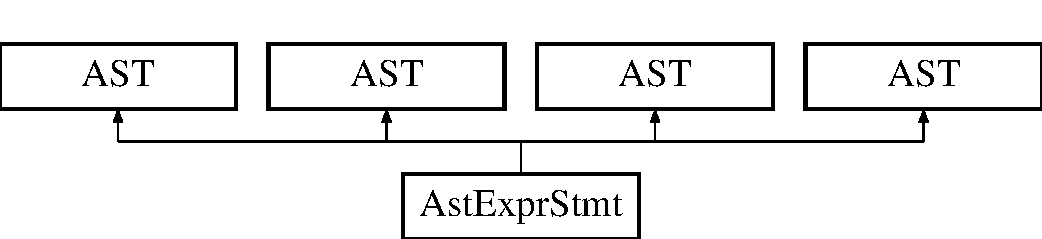
\includegraphics[height=2.000000cm]{classAstExprStmt}
\end{center}
\end{figure}
\subsection*{Public Member Functions}
\begin{DoxyCompactItemize}
\item 
\hypertarget{classAstExprStmt_a1ae9430bd6b1d01b6e3df6924012af56}{{\bfseries Ast\-Expr\-Stmt} (\hyperlink{classAstExpression}{Ast\-Expression} $\ast$e)}\label{classAstExprStmt_a1ae9430bd6b1d01b6e3df6924012af56}

\item 
void \hyperlink{classAstExprStmt_aa6763a98f7659d35edf7cf60557609b2}{Visit} ()
\begin{DoxyCompactList}\small\item\em This function is responsible for tree traversals. \end{DoxyCompactList}\item 
\hypertarget{classAstExprStmt_a1ae9430bd6b1d01b6e3df6924012af56}{{\bfseries Ast\-Expr\-Stmt} (\hyperlink{classAstExpression}{Ast\-Expression} $\ast$e)}\label{classAstExprStmt_a1ae9430bd6b1d01b6e3df6924012af56}

\item 
void \hyperlink{classAstExprStmt_aa6763a98f7659d35edf7cf60557609b2}{Visit} ()
\begin{DoxyCompactList}\small\item\em This function is responsible for tree traversals. \end{DoxyCompactList}\item 
\hypertarget{classAstExprStmt_a1ae9430bd6b1d01b6e3df6924012af56}{{\bfseries Ast\-Expr\-Stmt} (\hyperlink{classAstExpression}{Ast\-Expression} $\ast$e)}\label{classAstExprStmt_a1ae9430bd6b1d01b6e3df6924012af56}

\item 
void \hyperlink{classAstExprStmt_aa6763a98f7659d35edf7cf60557609b2}{Visit} ()
\begin{DoxyCompactList}\small\item\em This function is responsible for tree traversals. \end{DoxyCompactList}\item 
\hypertarget{classAstExprStmt_a1ae9430bd6b1d01b6e3df6924012af56}{{\bfseries Ast\-Expr\-Stmt} (\hyperlink{classAstExpression}{Ast\-Expression} $\ast$e)}\label{classAstExprStmt_a1ae9430bd6b1d01b6e3df6924012af56}

\item 
void \hyperlink{classAstExprStmt_aa6763a98f7659d35edf7cf60557609b2}{Visit} ()
\begin{DoxyCompactList}\small\item\em This function is responsible for tree traversals. \end{DoxyCompactList}\item 
void \hyperlink{classAST_a71d680856e95ff89f55d5311a552eba6}{set\-Label} (string l)
\begin{DoxyCompactList}\small\item\em Sets the label for the node. \end{DoxyCompactList}\item 
void \hyperlink{classAST_a71d680856e95ff89f55d5311a552eba6}{set\-Label} (string l)
\begin{DoxyCompactList}\small\item\em Sets the label for the node. \end{DoxyCompactList}\item 
void \hyperlink{classAST_a71d680856e95ff89f55d5311a552eba6}{set\-Label} (string l)
\begin{DoxyCompactList}\small\item\em Sets the label for the node. \end{DoxyCompactList}\item 
void \hyperlink{classAST_a71d680856e95ff89f55d5311a552eba6}{set\-Label} (string l)
\begin{DoxyCompactList}\small\item\em Sets the label for the node. \end{DoxyCompactList}\item 
int \hyperlink{classAST_ab7a5b1d9f1c2de0d98deb356f724a42c}{get\-U\-I\-D} ()
\begin{DoxyCompactList}\small\item\em Gets the node's unique I\-D. \end{DoxyCompactList}\item 
int \hyperlink{classAST_ab7a5b1d9f1c2de0d98deb356f724a42c}{get\-U\-I\-D} ()
\begin{DoxyCompactList}\small\item\em Gets the node's unique I\-D. \end{DoxyCompactList}\item 
int \hyperlink{classAST_ab7a5b1d9f1c2de0d98deb356f724a42c}{get\-U\-I\-D} ()
\begin{DoxyCompactList}\small\item\em Gets the node's unique I\-D. \end{DoxyCompactList}\item 
int \hyperlink{classAST_ab7a5b1d9f1c2de0d98deb356f724a42c}{get\-U\-I\-D} ()
\begin{DoxyCompactList}\small\item\em Gets the node's unique I\-D. \end{DoxyCompactList}\item 
string \hyperlink{classAST_aee029be902fffc927d16ccb03eb922ad}{get\-Label} ()
\begin{DoxyCompactList}\small\item\em Gets the node's label. \end{DoxyCompactList}\item 
string \hyperlink{classAST_aee029be902fffc927d16ccb03eb922ad}{get\-Label} ()
\begin{DoxyCompactList}\small\item\em Gets the node's label. \end{DoxyCompactList}\item 
string \hyperlink{classAST_aee029be902fffc927d16ccb03eb922ad}{get\-Label} ()
\begin{DoxyCompactList}\small\item\em Gets the node's label. \end{DoxyCompactList}\item 
string \hyperlink{classAST_aee029be902fffc927d16ccb03eb922ad}{get\-Label} ()
\begin{DoxyCompactList}\small\item\em Gets the node's label. \end{DoxyCompactList}\end{DoxyCompactItemize}
\subsection*{Public Attributes}
\begin{DoxyCompactItemize}
\item 
\hypertarget{classAST_aaf215802de409f8096c063d01ffa6783}{bool \hyperlink{classAST_aaf215802de409f8096c063d01ffa6783}{needs\-Cast}}\label{classAST_aaf215802de409f8096c063d01ffa6783}

\begin{DoxyCompactList}\small\item\em This indicates if cast 3\-A\-C needs to be output, and is only relevant for expressions. \end{DoxyCompactList}\item 
\hypertarget{classAST_afa9e77ef650ec6664458fa6cb55be985}{bool \hyperlink{classAST_afa9e77ef650ec6664458fa6cb55be985}{is\-Conv}}\label{classAST_afa9e77ef650ec6664458fa6cb55be985}

\begin{DoxyCompactList}\small\item\em Indicates is a conversion is possible. \end{DoxyCompactList}\item 
\hypertarget{classAST_a61ef3317e023d45237e06615b387cd6b}{C\-O\-N\-V\-E\-R\-S\-I\-O\-N\-T\-Y\-P\-E \hyperlink{classAST_a61ef3317e023d45237e06615b387cd6b}{conv\-Type}}\label{classAST_a61ef3317e023d45237e06615b387cd6b}

\begin{DoxyCompactList}\small\item\em If needs\-Cast is true, then this indicates what the cast should be. \end{DoxyCompactList}\item 
\hypertarget{classAST_aea9b07b39d24183f38c0029cec0a878e}{int \hyperlink{classAST_aea9b07b39d24183f38c0029cec0a878e}{operand\-To\-Cast}}\label{classAST_aea9b07b39d24183f38c0029cec0a878e}

\begin{DoxyCompactList}\small\item\em This indicates if the first or second operand should be the one that is cast. \end{DoxyCompactList}\end{DoxyCompactItemize}
\subsection*{Static Public Attributes}
\begin{DoxyCompactItemize}
\item 
\hypertarget{classAST_a5fdfd5f7b104dd92889163bdadbc68d6}{static \hyperlink{classVisualizer}{Visualizer} \hyperlink{classAST_a5fdfd5f7b104dd92889163bdadbc68d6}{vis}}\label{classAST_a5fdfd5f7b104dd92889163bdadbc68d6}

\begin{DoxyCompactList}\small\item\em Static visualizer instance for generating the visualization of the \hyperlink{classAST}{A\-S\-T}. \end{DoxyCompactList}\item 
\hypertarget{classAST_a8a3ace322f50e030331065d644ee55ee}{static \hyperlink{classTAC__Generator}{T\-A\-C\-\_\-\-Generator} \hyperlink{classAST_a8a3ace322f50e030331065d644ee55ee}{tac\-Gen}}\label{classAST_a8a3ace322f50e030331065d644ee55ee}

\begin{DoxyCompactList}\small\item\em Three address code generator. \end{DoxyCompactList}\item 
\hypertarget{classAST_a1f69448c6dc368d005631a128460083d}{static string {\bfseries current\-Temp} =\char`\"{}\char`\"{}}\label{classAST_a1f69448c6dc368d005631a128460083d}

\item 
\hypertarget{classAST_a551aec090c932ab69365238b40a8a4eb}{static string \hyperlink{classAST_a551aec090c932ab69365238b40a8a4eb}{return\-Label} =\char`\"{}\char`\"{}}\label{classAST_a551aec090c932ab69365238b40a8a4eb}

\begin{DoxyCompactList}\small\item\em This is for storing the string id of any temporary result register that may be created during 3\-A\-C generation. \end{DoxyCompactList}\item 
\hypertarget{classAST_a73c0a266df52be71e6b527b6aa635173}{static list$<$ string $>$ {\bfseries temp\-Stack}}\label{classAST_a73c0a266df52be71e6b527b6aa635173}

\item 
\hypertarget{classAST_abf9e84b541ff04b7bb64e6e4371512d4}{static string {\bfseries last\-I\-D} =\char`\"{}\char`\"{}}\label{classAST_abf9e84b541ff04b7bb64e6e4371512d4}

\item 
\hypertarget{classAST_a163003bfe9c30510ec8039870346049f}{static \hyperlink{classSymTab}{Sym\-Tab} $\ast$ {\bfseries symbol\-Table} =N\-U\-L\-L}\label{classAST_a163003bfe9c30510ec8039870346049f}

\item 
\hypertarget{classAST_a5c3cc894d9c0453523dec9ed76f18a04}{static string {\bfseries current\-Function} =\char`\"{}\char`\"{}}\label{classAST_a5c3cc894d9c0453523dec9ed76f18a04}

\end{DoxyCompactItemize}
\subsection*{Protected Attributes}
\begin{DoxyCompactItemize}
\item 
\hypertarget{classAST_a847b778f1c3dd5a19de32de432ee6e15}{int \hyperlink{classAST_a847b778f1c3dd5a19de32de432ee6e15}{uid}}\label{classAST_a847b778f1c3dd5a19de32de432ee6e15}

\begin{DoxyCompactList}\small\item\em The unique id. \end{DoxyCompactList}\item 
\hypertarget{classAST_ab2e239ccc0688d2341724432ff5a1a31}{string \hyperlink{classAST_ab2e239ccc0688d2341724432ff5a1a31}{label}}\label{classAST_ab2e239ccc0688d2341724432ff5a1a31}

\begin{DoxyCompactList}\small\item\em The label to be printed in the visualization. \end{DoxyCompactList}\end{DoxyCompactItemize}
\subsection*{Private Attributes}
\begin{DoxyCompactItemize}
\item 
\hypertarget{classAstExprStmt_a65a334737f1d579ff890c46ea4a91777}{\hyperlink{classAstExpression}{Ast\-Expression} $\ast$ {\bfseries expr}}\label{classAstExprStmt_a65a334737f1d579ff890c46ea4a91777}

\end{DoxyCompactItemize}


\subsection{Detailed Description}


Definition at line 804 of file Ast.\-h.



\subsection{Member Function Documentation}
\hypertarget{classAST_aee029be902fffc927d16ccb03eb922ad}{\index{Ast\-Expr\-Stmt@{Ast\-Expr\-Stmt}!get\-Label@{get\-Label}}
\index{get\-Label@{get\-Label}!AstExprStmt@{Ast\-Expr\-Stmt}}
\subsubsection[{get\-Label}]{\setlength{\rightskip}{0pt plus 5cm}string A\-S\-T\-::get\-Label (
\begin{DoxyParamCaption}
{}
\end{DoxyParamCaption}
)\hspace{0.3cm}{\ttfamily [inline]}, {\ttfamily [inherited]}}}\label{classAST_aee029be902fffc927d16ccb03eb922ad}


Gets the node's label. 

\begin{DoxyReturn}{Returns}
The label 
\end{DoxyReturn}


Definition at line 60 of file Ast.\-h.

\hypertarget{classAST_aee029be902fffc927d16ccb03eb922ad}{\index{Ast\-Expr\-Stmt@{Ast\-Expr\-Stmt}!get\-Label@{get\-Label}}
\index{get\-Label@{get\-Label}!AstExprStmt@{Ast\-Expr\-Stmt}}
\subsubsection[{get\-Label}]{\setlength{\rightskip}{0pt plus 5cm}string A\-S\-T\-::get\-Label (
\begin{DoxyParamCaption}
{}
\end{DoxyParamCaption}
)\hspace{0.3cm}{\ttfamily [inline]}, {\ttfamily [inherited]}}}\label{classAST_aee029be902fffc927d16ccb03eb922ad}


Gets the node's label. 

\begin{DoxyReturn}{Returns}
The label 
\end{DoxyReturn}


Definition at line 60 of file C\-Scanner.\-ll.

\hypertarget{classAST_aee029be902fffc927d16ccb03eb922ad}{\index{Ast\-Expr\-Stmt@{Ast\-Expr\-Stmt}!get\-Label@{get\-Label}}
\index{get\-Label@{get\-Label}!AstExprStmt@{Ast\-Expr\-Stmt}}
\subsubsection[{get\-Label}]{\setlength{\rightskip}{0pt plus 5cm}string A\-S\-T\-::get\-Label (
\begin{DoxyParamCaption}
{}
\end{DoxyParamCaption}
)\hspace{0.3cm}{\ttfamily [inline]}, {\ttfamily [inherited]}}}\label{classAST_aee029be902fffc927d16ccb03eb922ad}


Gets the node's label. 

\begin{DoxyReturn}{Returns}
The label 
\end{DoxyReturn}


Definition at line 60 of file C\-Parser.\-yy.

\hypertarget{classAST_aee029be902fffc927d16ccb03eb922ad}{\index{Ast\-Expr\-Stmt@{Ast\-Expr\-Stmt}!get\-Label@{get\-Label}}
\index{get\-Label@{get\-Label}!AstExprStmt@{Ast\-Expr\-Stmt}}
\subsubsection[{get\-Label}]{\setlength{\rightskip}{0pt plus 5cm}string A\-S\-T\-::get\-Label (
\begin{DoxyParamCaption}
{}
\end{DoxyParamCaption}
)\hspace{0.3cm}{\ttfamily [inline]}, {\ttfamily [inherited]}}}\label{classAST_aee029be902fffc927d16ccb03eb922ad}


Gets the node's label. 

\begin{DoxyReturn}{Returns}
The label 
\end{DoxyReturn}


Definition at line 60 of file C\-Parser.\-yy.

\hypertarget{classAST_ab7a5b1d9f1c2de0d98deb356f724a42c}{\index{Ast\-Expr\-Stmt@{Ast\-Expr\-Stmt}!get\-U\-I\-D@{get\-U\-I\-D}}
\index{get\-U\-I\-D@{get\-U\-I\-D}!AstExprStmt@{Ast\-Expr\-Stmt}}
\subsubsection[{get\-U\-I\-D}]{\setlength{\rightskip}{0pt plus 5cm}int A\-S\-T\-::get\-U\-I\-D (
\begin{DoxyParamCaption}
{}
\end{DoxyParamCaption}
)\hspace{0.3cm}{\ttfamily [inline]}, {\ttfamily [inherited]}}}\label{classAST_ab7a5b1d9f1c2de0d98deb356f724a42c}


Gets the node's unique I\-D. 

\begin{DoxyReturn}{Returns}
The unique id 
\end{DoxyReturn}


Definition at line 53 of file C\-Parser.\-yy.

\hypertarget{classAST_ab7a5b1d9f1c2de0d98deb356f724a42c}{\index{Ast\-Expr\-Stmt@{Ast\-Expr\-Stmt}!get\-U\-I\-D@{get\-U\-I\-D}}
\index{get\-U\-I\-D@{get\-U\-I\-D}!AstExprStmt@{Ast\-Expr\-Stmt}}
\subsubsection[{get\-U\-I\-D}]{\setlength{\rightskip}{0pt plus 5cm}int A\-S\-T\-::get\-U\-I\-D (
\begin{DoxyParamCaption}
{}
\end{DoxyParamCaption}
)\hspace{0.3cm}{\ttfamily [inline]}, {\ttfamily [inherited]}}}\label{classAST_ab7a5b1d9f1c2de0d98deb356f724a42c}


Gets the node's unique I\-D. 

\begin{DoxyReturn}{Returns}
The unique id 
\end{DoxyReturn}


Definition at line 53 of file C\-Parser.\-yy.

\hypertarget{classAST_ab7a5b1d9f1c2de0d98deb356f724a42c}{\index{Ast\-Expr\-Stmt@{Ast\-Expr\-Stmt}!get\-U\-I\-D@{get\-U\-I\-D}}
\index{get\-U\-I\-D@{get\-U\-I\-D}!AstExprStmt@{Ast\-Expr\-Stmt}}
\subsubsection[{get\-U\-I\-D}]{\setlength{\rightskip}{0pt plus 5cm}int A\-S\-T\-::get\-U\-I\-D (
\begin{DoxyParamCaption}
{}
\end{DoxyParamCaption}
)\hspace{0.3cm}{\ttfamily [inline]}, {\ttfamily [inherited]}}}\label{classAST_ab7a5b1d9f1c2de0d98deb356f724a42c}


Gets the node's unique I\-D. 

\begin{DoxyReturn}{Returns}
The unique id 
\end{DoxyReturn}


Definition at line 53 of file C\-Scanner.\-ll.

\hypertarget{classAST_ab7a5b1d9f1c2de0d98deb356f724a42c}{\index{Ast\-Expr\-Stmt@{Ast\-Expr\-Stmt}!get\-U\-I\-D@{get\-U\-I\-D}}
\index{get\-U\-I\-D@{get\-U\-I\-D}!AstExprStmt@{Ast\-Expr\-Stmt}}
\subsubsection[{get\-U\-I\-D}]{\setlength{\rightskip}{0pt plus 5cm}int A\-S\-T\-::get\-U\-I\-D (
\begin{DoxyParamCaption}
{}
\end{DoxyParamCaption}
)\hspace{0.3cm}{\ttfamily [inline]}, {\ttfamily [inherited]}}}\label{classAST_ab7a5b1d9f1c2de0d98deb356f724a42c}


Gets the node's unique I\-D. 

\begin{DoxyReturn}{Returns}
The unique id 
\end{DoxyReturn}


Definition at line 53 of file Ast.\-h.

\hypertarget{classAST_a71d680856e95ff89f55d5311a552eba6}{\index{Ast\-Expr\-Stmt@{Ast\-Expr\-Stmt}!set\-Label@{set\-Label}}
\index{set\-Label@{set\-Label}!AstExprStmt@{Ast\-Expr\-Stmt}}
\subsubsection[{set\-Label}]{\setlength{\rightskip}{0pt plus 5cm}void A\-S\-T\-::set\-Label (
\begin{DoxyParamCaption}
\item[{string}]{l}
\end{DoxyParamCaption}
)\hspace{0.3cm}{\ttfamily [inline]}, {\ttfamily [inherited]}}}\label{classAST_a71d680856e95ff89f55d5311a552eba6}


Sets the label for the node. 


\begin{DoxyParams}{Parameters}
{\em l} & The label string \\
\hline
\end{DoxyParams}


Definition at line 43 of file C\-Scanner.\-ll.

\hypertarget{classAST_a71d680856e95ff89f55d5311a552eba6}{\index{Ast\-Expr\-Stmt@{Ast\-Expr\-Stmt}!set\-Label@{set\-Label}}
\index{set\-Label@{set\-Label}!AstExprStmt@{Ast\-Expr\-Stmt}}
\subsubsection[{set\-Label}]{\setlength{\rightskip}{0pt plus 5cm}void A\-S\-T\-::set\-Label (
\begin{DoxyParamCaption}
\item[{string}]{l}
\end{DoxyParamCaption}
)\hspace{0.3cm}{\ttfamily [inline]}, {\ttfamily [inherited]}}}\label{classAST_a71d680856e95ff89f55d5311a552eba6}


Sets the label for the node. 


\begin{DoxyParams}{Parameters}
{\em l} & The label string \\
\hline
\end{DoxyParams}


Definition at line 43 of file C\-Parser.\-yy.

\hypertarget{classAST_a71d680856e95ff89f55d5311a552eba6}{\index{Ast\-Expr\-Stmt@{Ast\-Expr\-Stmt}!set\-Label@{set\-Label}}
\index{set\-Label@{set\-Label}!AstExprStmt@{Ast\-Expr\-Stmt}}
\subsubsection[{set\-Label}]{\setlength{\rightskip}{0pt plus 5cm}void A\-S\-T\-::set\-Label (
\begin{DoxyParamCaption}
\item[{string}]{l}
\end{DoxyParamCaption}
)\hspace{0.3cm}{\ttfamily [inline]}, {\ttfamily [inherited]}}}\label{classAST_a71d680856e95ff89f55d5311a552eba6}


Sets the label for the node. 


\begin{DoxyParams}{Parameters}
{\em l} & The label string \\
\hline
\end{DoxyParams}


Definition at line 43 of file Ast.\-h.

\hypertarget{classAST_a71d680856e95ff89f55d5311a552eba6}{\index{Ast\-Expr\-Stmt@{Ast\-Expr\-Stmt}!set\-Label@{set\-Label}}
\index{set\-Label@{set\-Label}!AstExprStmt@{Ast\-Expr\-Stmt}}
\subsubsection[{set\-Label}]{\setlength{\rightskip}{0pt plus 5cm}void A\-S\-T\-::set\-Label (
\begin{DoxyParamCaption}
\item[{string}]{l}
\end{DoxyParamCaption}
)\hspace{0.3cm}{\ttfamily [inline]}, {\ttfamily [inherited]}}}\label{classAST_a71d680856e95ff89f55d5311a552eba6}


Sets the label for the node. 


\begin{DoxyParams}{Parameters}
{\em l} & The label string \\
\hline
\end{DoxyParams}


Definition at line 43 of file C\-Parser.\-yy.

\hypertarget{classAstExprStmt_aa6763a98f7659d35edf7cf60557609b2}{\index{Ast\-Expr\-Stmt@{Ast\-Expr\-Stmt}!Visit@{Visit}}
\index{Visit@{Visit}!AstExprStmt@{Ast\-Expr\-Stmt}}
\subsubsection[{Visit}]{\setlength{\rightskip}{0pt plus 5cm}void Ast\-Expr\-Stmt\-::\-Visit (
\begin{DoxyParamCaption}
{}
\end{DoxyParamCaption}
)\hspace{0.3cm}{\ttfamily [virtual]}}}\label{classAstExprStmt_aa6763a98f7659d35edf7cf60557609b2}


This function is responsible for tree traversals. 

This function will call the Visit functions of each of it's children nodes, call the visualization code for itself, and output any 3\-A\-C that can be generated at the current node. 

Reimplemented from \hyperlink{classAST_a5828cc86f2c4f1a0aeab6d7069e8fd82}{A\-S\-T}.



Definition at line 2473 of file Ast.\-cpp.

\hypertarget{classAstExprStmt_aa6763a98f7659d35edf7cf60557609b2}{\index{Ast\-Expr\-Stmt@{Ast\-Expr\-Stmt}!Visit@{Visit}}
\index{Visit@{Visit}!AstExprStmt@{Ast\-Expr\-Stmt}}
\subsubsection[{Visit}]{\setlength{\rightskip}{0pt plus 5cm}void Ast\-Expr\-Stmt\-::\-Visit (
\begin{DoxyParamCaption}
{}
\end{DoxyParamCaption}
)\hspace{0.3cm}{\ttfamily [virtual]}}}\label{classAstExprStmt_aa6763a98f7659d35edf7cf60557609b2}


This function is responsible for tree traversals. 

This function will call the Visit functions of each of it's children nodes, call the visualization code for itself, and output any 3\-A\-C that can be generated at the current node. 

Reimplemented from \hyperlink{classAST_a5828cc86f2c4f1a0aeab6d7069e8fd82}{A\-S\-T}.

\hypertarget{classAstExprStmt_aa6763a98f7659d35edf7cf60557609b2}{\index{Ast\-Expr\-Stmt@{Ast\-Expr\-Stmt}!Visit@{Visit}}
\index{Visit@{Visit}!AstExprStmt@{Ast\-Expr\-Stmt}}
\subsubsection[{Visit}]{\setlength{\rightskip}{0pt plus 5cm}void Ast\-Expr\-Stmt\-::\-Visit (
\begin{DoxyParamCaption}
{}
\end{DoxyParamCaption}
)\hspace{0.3cm}{\ttfamily [virtual]}}}\label{classAstExprStmt_aa6763a98f7659d35edf7cf60557609b2}


This function is responsible for tree traversals. 

This function will call the Visit functions of each of it's children nodes, call the visualization code for itself, and output any 3\-A\-C that can be generated at the current node. 

Reimplemented from \hyperlink{classAST_a5828cc86f2c4f1a0aeab6d7069e8fd82}{A\-S\-T}.

\hypertarget{classAstExprStmt_aa6763a98f7659d35edf7cf60557609b2}{\index{Ast\-Expr\-Stmt@{Ast\-Expr\-Stmt}!Visit@{Visit}}
\index{Visit@{Visit}!AstExprStmt@{Ast\-Expr\-Stmt}}
\subsubsection[{Visit}]{\setlength{\rightskip}{0pt plus 5cm}void Ast\-Expr\-Stmt\-::\-Visit (
\begin{DoxyParamCaption}
{}
\end{DoxyParamCaption}
)\hspace{0.3cm}{\ttfamily [virtual]}}}\label{classAstExprStmt_aa6763a98f7659d35edf7cf60557609b2}


This function is responsible for tree traversals. 

This function will call the Visit functions of each of it's children nodes, call the visualization code for itself, and output any 3\-A\-C that can be generated at the current node. 

Reimplemented from \hyperlink{classAST_a5828cc86f2c4f1a0aeab6d7069e8fd82}{A\-S\-T}.



The documentation for this class was generated from the following files\-:\begin{DoxyCompactItemize}
\item 
Ast.\-h\item 
Ast.\-cpp\end{DoxyCompactItemize}

\hypertarget{classAstFor}{\section{Ast\-For Class Reference}
\label{classAstFor}\index{Ast\-For@{Ast\-For}}
}
Inheritance diagram for Ast\-For\-:\begin{figure}[H]
\begin{center}
\leavevmode
\includegraphics[height=2.000000cm]{classAstFor}
\end{center}
\end{figure}
\subsection*{Public Member Functions}
\begin{DoxyCompactItemize}
\item 
\hypertarget{classAstFor_af4b510c833d8cb2b64e5ba1d700b6e1b}{{\bfseries Ast\-For} (\hyperlink{classAstExpression}{Ast\-Expression} $\ast$init, \hyperlink{classAstExpression}{Ast\-Expression} $\ast$test, \hyperlink{classAstExpression}{Ast\-Expression} $\ast$increment, \hyperlink{classAstStatement}{Ast\-Statement} $\ast$statement)}\label{classAstFor_af4b510c833d8cb2b64e5ba1d700b6e1b}

\item 
\hypertarget{classAstFor_aabb94ea30de2b634b35c02ec3688d0ff}{void {\bfseries Visit} ()}\label{classAstFor_aabb94ea30de2b634b35c02ec3688d0ff}

\item 
\hypertarget{classAST_a71d680856e95ff89f55d5311a552eba6}{void {\bfseries set\-Label} (string l)}\label{classAST_a71d680856e95ff89f55d5311a552eba6}

\item 
\hypertarget{classAST_ab7a5b1d9f1c2de0d98deb356f724a42c}{int {\bfseries get\-U\-I\-D} ()}\label{classAST_ab7a5b1d9f1c2de0d98deb356f724a42c}

\item 
\hypertarget{classAST_aee029be902fffc927d16ccb03eb922ad}{string {\bfseries get\-Label} ()}\label{classAST_aee029be902fffc927d16ccb03eb922ad}

\end{DoxyCompactItemize}
\subsection*{Static Public Attributes}
\begin{DoxyCompactItemize}
\item 
\hypertarget{classAST_aca9e6637209b31e03a09c0d42f29bdfa}{static \hyperlink{classVisualizer}{Visualizer} {\bfseries vis}}\label{classAST_aca9e6637209b31e03a09c0d42f29bdfa}

\end{DoxyCompactItemize}
\subsection*{Protected Attributes}
\begin{DoxyCompactItemize}
\item 
\hypertarget{classAST_a847b778f1c3dd5a19de32de432ee6e15}{int {\bfseries uid}}\label{classAST_a847b778f1c3dd5a19de32de432ee6e15}

\item 
\hypertarget{classAST_ab2e239ccc0688d2341724432ff5a1a31}{string {\bfseries label}}\label{classAST_ab2e239ccc0688d2341724432ff5a1a31}

\end{DoxyCompactItemize}
\subsection*{Private Attributes}
\begin{DoxyCompactItemize}
\item 
\hypertarget{classAstFor_aaebd550fca64ada15ccd61f784a7b8e3}{\hyperlink{classAstExpression}{Ast\-Expression} $\ast$ {\bfseries init}}\label{classAstFor_aaebd550fca64ada15ccd61f784a7b8e3}

\item 
\hypertarget{classAstFor_abc2bfc9976f254069d7f80db22630ada}{\hyperlink{classAstExpression}{Ast\-Expression} $\ast$ {\bfseries test}}\label{classAstFor_abc2bfc9976f254069d7f80db22630ada}

\item 
\hypertarget{classAstFor_a4638ba73c928d6144972acc06b8226f8}{\hyperlink{classAstExpression}{Ast\-Expression} $\ast$ {\bfseries increment}}\label{classAstFor_a4638ba73c928d6144972acc06b8226f8}

\item 
\hypertarget{classAstFor_a9d7943f531d80a986672c55100da1a0f}{\hyperlink{classAstStatement}{Ast\-Statement} $\ast$ {\bfseries statement}}\label{classAstFor_a9d7943f531d80a986672c55100da1a0f}

\end{DoxyCompactItemize}


The documentation for this class was generated from the following files\-:\begin{DoxyCompactItemize}
\item 
Ast.\-h\item 
Ast.\-cpp\end{DoxyCompactItemize}

\input{classAstFuncDef}
\hypertarget{classAstGoto}{\section{Ast\-Goto Class Reference}
\label{classAstGoto}\index{Ast\-Goto@{Ast\-Goto}}
}
Inheritance diagram for Ast\-Goto\-:\begin{figure}[H]
\begin{center}
\leavevmode
\includegraphics[height=2.000000cm]{classAstGoto}
\end{center}
\end{figure}
\subsection*{Public Member Functions}
\begin{DoxyCompactItemize}
\item 
\hypertarget{classAstGoto_aa74c48ee01065e4cc79f686bdcfff22a}{void {\bfseries Visit} ()}\label{classAstGoto_aa74c48ee01065e4cc79f686bdcfff22a}

\item 
\hypertarget{classAST_a71d680856e95ff89f55d5311a552eba6}{void {\bfseries set\-Label} (string l)}\label{classAST_a71d680856e95ff89f55d5311a552eba6}

\item 
\hypertarget{classAST_ab7a5b1d9f1c2de0d98deb356f724a42c}{int {\bfseries get\-U\-I\-D} ()}\label{classAST_ab7a5b1d9f1c2de0d98deb356f724a42c}

\item 
\hypertarget{classAST_aee029be902fffc927d16ccb03eb922ad}{string {\bfseries get\-Label} ()}\label{classAST_aee029be902fffc927d16ccb03eb922ad}

\end{DoxyCompactItemize}
\subsection*{Static Public Attributes}
\begin{DoxyCompactItemize}
\item 
\hypertarget{classAST_aca9e6637209b31e03a09c0d42f29bdfa}{static \hyperlink{classVisualizer}{Visualizer} {\bfseries vis}}\label{classAST_aca9e6637209b31e03a09c0d42f29bdfa}

\end{DoxyCompactItemize}
\subsection*{Protected Attributes}
\begin{DoxyCompactItemize}
\item 
\hypertarget{classAST_a847b778f1c3dd5a19de32de432ee6e15}{int {\bfseries uid}}\label{classAST_a847b778f1c3dd5a19de32de432ee6e15}

\item 
\hypertarget{classAST_ab2e239ccc0688d2341724432ff5a1a31}{string {\bfseries label}}\label{classAST_ab2e239ccc0688d2341724432ff5a1a31}

\end{DoxyCompactItemize}


The documentation for this class was generated from the following files\-:\begin{DoxyCompactItemize}
\item 
Ast.\-h\item 
Ast.\-cpp\end{DoxyCompactItemize}

\input{classAstID}
\input{classAstIDList}
\hypertarget{classAstIfElse}{\section{Ast\-If\-Else Class Reference}
\label{classAstIfElse}\index{Ast\-If\-Else@{Ast\-If\-Else}}
}
Inheritance diagram for Ast\-If\-Else\-:\begin{figure}[H]
\begin{center}
\leavevmode
\includegraphics[height=2.000000cm]{classAstIfElse}
\end{center}
\end{figure}
\subsection*{Public Member Functions}
\begin{DoxyCompactItemize}
\item 
\hypertarget{classAstIfElse_aac4a0ab9c36999fdd491ef5fe6c1e68c}{{\bfseries Ast\-If\-Else} (\hyperlink{classAstExpression}{Ast\-Expression} $\ast$test, \hyperlink{classAstStatement}{Ast\-Statement} $\ast$statement, \hyperlink{classAstStatement}{Ast\-Statement} $\ast$else\-Statement)}\label{classAstIfElse_aac4a0ab9c36999fdd491ef5fe6c1e68c}

\item 
\hypertarget{classAstIfElse_a4c038fd5b0cb99ea75f9847d96f65c32}{void {\bfseries Visit} ()}\label{classAstIfElse_a4c038fd5b0cb99ea75f9847d96f65c32}

\item 
\hypertarget{classAST_a71d680856e95ff89f55d5311a552eba6}{void {\bfseries set\-Label} (string l)}\label{classAST_a71d680856e95ff89f55d5311a552eba6}

\item 
\hypertarget{classAST_ab7a5b1d9f1c2de0d98deb356f724a42c}{int {\bfseries get\-U\-I\-D} ()}\label{classAST_ab7a5b1d9f1c2de0d98deb356f724a42c}

\item 
\hypertarget{classAST_aee029be902fffc927d16ccb03eb922ad}{string {\bfseries get\-Label} ()}\label{classAST_aee029be902fffc927d16ccb03eb922ad}

\end{DoxyCompactItemize}
\subsection*{Static Public Attributes}
\begin{DoxyCompactItemize}
\item 
\hypertarget{classAST_aca9e6637209b31e03a09c0d42f29bdfa}{static \hyperlink{classVisualizer}{Visualizer} {\bfseries vis}}\label{classAST_aca9e6637209b31e03a09c0d42f29bdfa}

\end{DoxyCompactItemize}
\subsection*{Protected Attributes}
\begin{DoxyCompactItemize}
\item 
\hypertarget{classAST_a847b778f1c3dd5a19de32de432ee6e15}{int {\bfseries uid}}\label{classAST_a847b778f1c3dd5a19de32de432ee6e15}

\item 
\hypertarget{classAST_ab2e239ccc0688d2341724432ff5a1a31}{string {\bfseries label}}\label{classAST_ab2e239ccc0688d2341724432ff5a1a31}

\end{DoxyCompactItemize}
\subsection*{Private Attributes}
\begin{DoxyCompactItemize}
\item 
\hypertarget{classAstIfElse_a8ee373b9a53acbc71387f948beb335a7}{\hyperlink{classAstExpression}{Ast\-Expression} $\ast$ {\bfseries test}}\label{classAstIfElse_a8ee373b9a53acbc71387f948beb335a7}

\item 
\hypertarget{classAstIfElse_ab9af93616039b05a021413df65896f1c}{\hyperlink{classAstStatement}{Ast\-Statement} $\ast$ {\bfseries statement}}\label{classAstIfElse_ab9af93616039b05a021413df65896f1c}

\item 
\hypertarget{classAstIfElse_aa6d9b8e028316ba27da5ad73729f9169}{\hyperlink{classAstStatement}{Ast\-Statement} $\ast$ {\bfseries else\-Statement}}\label{classAstIfElse_aa6d9b8e028316ba27da5ad73729f9169}

\end{DoxyCompactItemize}


The documentation for this class was generated from the following files\-:\begin{DoxyCompactItemize}
\item 
Ast.\-h\item 
Ast.\-cpp\end{DoxyCompactItemize}

\input{classAstInitDeclarator}
\input{classAstInitDeclList}
\input{classAstInitializer}
\input{classAstInitList}
\hypertarget{classAstIteration}{\section{Ast\-Iteration Class Reference}
\label{classAstIteration}\index{Ast\-Iteration@{Ast\-Iteration}}
}
Inheritance diagram for Ast\-Iteration\-:\begin{figure}[H]
\begin{center}
\leavevmode
\includegraphics[height=2.000000cm]{classAstIteration}
\end{center}
\end{figure}
\subsection*{Public Types}
\begin{DoxyCompactItemize}
\item 
enum {\bfseries Type} \{ {\bfseries D\-O\-W\-H\-I\-L\-E}, 
{\bfseries W\-H\-I\-L\-E}, 
{\bfseries F\-O\-R}
 \}
\end{DoxyCompactItemize}
\subsection*{Public Member Functions}
\begin{DoxyCompactItemize}
\item 
\hypertarget{classAstIteration_a9b98ddbdb8795a514c129a86fc00b561}{{\bfseries Ast\-Iteration} (\hyperlink{classAstDoWhile}{Ast\-Do\-While} $\ast$d)}\label{classAstIteration_a9b98ddbdb8795a514c129a86fc00b561}

\item 
\hypertarget{classAstIteration_aed79cf13c2e6376cab0a02b657ef6c87}{{\bfseries Ast\-Iteration} (\hyperlink{classAstWhile}{Ast\-While} $\ast$w)}\label{classAstIteration_aed79cf13c2e6376cab0a02b657ef6c87}

\item 
\hypertarget{classAstIteration_a87f1eaa5c3fc5b4562cbad3e54ff5061}{{\bfseries Ast\-Iteration} (\hyperlink{classAstFor}{Ast\-For} $\ast$f)}\label{classAstIteration_a87f1eaa5c3fc5b4562cbad3e54ff5061}

\item 
void \hyperlink{classAstIteration_ae3e90f781890621279ff29b5481e0d4b}{Visit} ()
\begin{DoxyCompactList}\small\item\em This function is responsible for tree traversals. \end{DoxyCompactList}\item 
void \hyperlink{classAST_a71d680856e95ff89f55d5311a552eba6}{set\-Label} (string l)
\begin{DoxyCompactList}\small\item\em Sets the label for the node. \end{DoxyCompactList}\item 
int \hyperlink{classAST_ab7a5b1d9f1c2de0d98deb356f724a42c}{get\-U\-I\-D} ()
\begin{DoxyCompactList}\small\item\em Gets the node's unique I\-D. \end{DoxyCompactList}\item 
string \hyperlink{classAST_aee029be902fffc927d16ccb03eb922ad}{get\-Label} ()
\begin{DoxyCompactList}\small\item\em Gets the node's label. \end{DoxyCompactList}\end{DoxyCompactItemize}
\subsection*{Public Attributes}
\begin{DoxyCompactItemize}
\item 
\hypertarget{classAstIteration_a41e8a7f05a840d8ddd333830f823314c}{enum Ast\-Iteration\-::\-Type {\bfseries t}}\label{classAstIteration_a41e8a7f05a840d8ddd333830f823314c}

\end{DoxyCompactItemize}
\subsection*{Static Public Attributes}
\begin{DoxyCompactItemize}
\item 
\hypertarget{classAST_aca9e6637209b31e03a09c0d42f29bdfa}{static \hyperlink{classVisualizer}{Visualizer} \hyperlink{classAST_aca9e6637209b31e03a09c0d42f29bdfa}{vis}}\label{classAST_aca9e6637209b31e03a09c0d42f29bdfa}

\begin{DoxyCompactList}\small\item\em Static visualizer instance for generating the visualization of the \hyperlink{classAST}{A\-S\-T}. \end{DoxyCompactList}\end{DoxyCompactItemize}
\subsection*{Protected Attributes}
\begin{DoxyCompactItemize}
\item 
\hypertarget{classAST_a847b778f1c3dd5a19de32de432ee6e15}{int \hyperlink{classAST_a847b778f1c3dd5a19de32de432ee6e15}{uid}}\label{classAST_a847b778f1c3dd5a19de32de432ee6e15}

\begin{DoxyCompactList}\small\item\em The unique id. \end{DoxyCompactList}\item 
\hypertarget{classAST_ab2e239ccc0688d2341724432ff5a1a31}{string \hyperlink{classAST_ab2e239ccc0688d2341724432ff5a1a31}{label}}\label{classAST_ab2e239ccc0688d2341724432ff5a1a31}

\begin{DoxyCompactList}\small\item\em The label to be printed in the visualization. \end{DoxyCompactList}\end{DoxyCompactItemize}
\subsection*{Private Attributes}
\begin{DoxyCompactItemize}
\item 
\hypertarget{classAstIteration_ac984b15a824002ce1825c942271a3020}{\hyperlink{classAstDoWhile}{Ast\-Do\-While} $\ast$ {\bfseries dwl}}\label{classAstIteration_ac984b15a824002ce1825c942271a3020}

\item 
\hypertarget{classAstIteration_aedd1375432ddac3f75b7abe71d7ba34a}{\hyperlink{classAstWhile}{Ast\-While} $\ast$ {\bfseries wl}}\label{classAstIteration_aedd1375432ddac3f75b7abe71d7ba34a}

\item 
\hypertarget{classAstIteration_a166639cd7bfababcd469b182d76be91f}{\hyperlink{classAstFor}{Ast\-For} $\ast$ {\bfseries fr}}\label{classAstIteration_a166639cd7bfababcd469b182d76be91f}

\end{DoxyCompactItemize}


\subsection{Member Function Documentation}
\hypertarget{classAST_aee029be902fffc927d16ccb03eb922ad}{\index{Ast\-Iteration@{Ast\-Iteration}!get\-Label@{get\-Label}}
\index{get\-Label@{get\-Label}!AstIteration@{Ast\-Iteration}}
\subsubsection[{get\-Label}]{\setlength{\rightskip}{0pt plus 5cm}string A\-S\-T\-::get\-Label (
\begin{DoxyParamCaption}
{}
\end{DoxyParamCaption}
)\hspace{0.3cm}{\ttfamily [inline]}, {\ttfamily [inherited]}}}\label{classAST_aee029be902fffc927d16ccb03eb922ad}


Gets the node's label. 

\begin{DoxyReturn}{Returns}
The label 
\end{DoxyReturn}
\hypertarget{classAST_ab7a5b1d9f1c2de0d98deb356f724a42c}{\index{Ast\-Iteration@{Ast\-Iteration}!get\-U\-I\-D@{get\-U\-I\-D}}
\index{get\-U\-I\-D@{get\-U\-I\-D}!AstIteration@{Ast\-Iteration}}
\subsubsection[{get\-U\-I\-D}]{\setlength{\rightskip}{0pt plus 5cm}int A\-S\-T\-::get\-U\-I\-D (
\begin{DoxyParamCaption}
{}
\end{DoxyParamCaption}
)\hspace{0.3cm}{\ttfamily [inline]}, {\ttfamily [inherited]}}}\label{classAST_ab7a5b1d9f1c2de0d98deb356f724a42c}


Gets the node's unique I\-D. 

\begin{DoxyReturn}{Returns}
The unique id 
\end{DoxyReturn}
\hypertarget{classAST_a71d680856e95ff89f55d5311a552eba6}{\index{Ast\-Iteration@{Ast\-Iteration}!set\-Label@{set\-Label}}
\index{set\-Label@{set\-Label}!AstIteration@{Ast\-Iteration}}
\subsubsection[{set\-Label}]{\setlength{\rightskip}{0pt plus 5cm}void A\-S\-T\-::set\-Label (
\begin{DoxyParamCaption}
\item[{string}]{l}
\end{DoxyParamCaption}
)\hspace{0.3cm}{\ttfamily [inline]}, {\ttfamily [inherited]}}}\label{classAST_a71d680856e95ff89f55d5311a552eba6}


Sets the label for the node. 


\begin{DoxyParams}{Parameters}
{\em l} & The label string \\
\hline
\end{DoxyParams}
\hypertarget{classAstIteration_ae3e90f781890621279ff29b5481e0d4b}{\index{Ast\-Iteration@{Ast\-Iteration}!Visit@{Visit}}
\index{Visit@{Visit}!AstIteration@{Ast\-Iteration}}
\subsubsection[{Visit}]{\setlength{\rightskip}{0pt plus 5cm}void Ast\-Iteration\-::\-Visit (
\begin{DoxyParamCaption}
{}
\end{DoxyParamCaption}
)\hspace{0.3cm}{\ttfamily [virtual]}}}\label{classAstIteration_ae3e90f781890621279ff29b5481e0d4b}


This function is responsible for tree traversals. 

This function will call the Visit functions of each of it's children nodes, call the visualization code for itself, and output any 3\-A\-C that can be generated at the current node. 

Reimplemented from \hyperlink{classAST_a5828cc86f2c4f1a0aeab6d7069e8fd82}{A\-S\-T}.



The documentation for this class was generated from the following files\-:\begin{DoxyCompactItemize}
\item 
Ast.\-h\item 
Ast.\-cpp\end{DoxyCompactItemize}

\hypertarget{classAstJump}{\section{Ast\-Jump Class Reference}
\label{classAstJump}\index{Ast\-Jump@{Ast\-Jump}}
}
Inheritance diagram for Ast\-Jump\-:\begin{figure}[H]
\begin{center}
\leavevmode
\includegraphics[height=2.000000cm]{classAstJump}
\end{center}
\end{figure}
\subsection*{Public Types}
\begin{DoxyCompactItemize}
\item 
enum {\bfseries Type} \{ \\*
{\bfseries G\-O\-T\-O}, 
{\bfseries C\-O\-N\-T\-I\-N\-U\-E}, 
{\bfseries B\-R\-E\-A\-K}, 
{\bfseries E\-M\-P\-T\-Y\-\_\-\-R\-E\-T\-U\-R\-N}, 
\\*
{\bfseries R\-E\-T\-U\-R\-N}
 \}
\end{DoxyCompactItemize}
\subsection*{Public Member Functions}
\begin{DoxyCompactItemize}
\item 
\hypertarget{classAstJump_a83a4aa905d84f3602374029976d99412}{{\bfseries Ast\-Jump} (\hyperlink{classAstGoto}{Ast\-Goto} $\ast$g, \hyperlink{classAstID}{Ast\-I\-D} $\ast$i)}\label{classAstJump_a83a4aa905d84f3602374029976d99412}

\item 
\hypertarget{classAstJump_a945a1bdc268bfa7f1fdd9f4d39bdef1a}{{\bfseries Ast\-Jump} (\hyperlink{classAstContinue}{Ast\-Continue} $\ast$c)}\label{classAstJump_a945a1bdc268bfa7f1fdd9f4d39bdef1a}

\item 
\hypertarget{classAstJump_a8b9e461b6a974f01889e89728afc7014}{{\bfseries Ast\-Jump} (\hyperlink{classAstBreak}{Ast\-Break} $\ast$b)}\label{classAstJump_a8b9e461b6a974f01889e89728afc7014}

\item 
\hypertarget{classAstJump_a083525b758ad6e931aee5ac850592730}{{\bfseries Ast\-Jump} (\hyperlink{classAstReturn}{Ast\-Return} $\ast$r)}\label{classAstJump_a083525b758ad6e931aee5ac850592730}

\item 
\hypertarget{classAstJump_ad80d35d23849aa369fef153fef4bb99e}{{\bfseries Ast\-Jump} (\hyperlink{classAstReturn}{Ast\-Return} $\ast$r, \hyperlink{classAstExpression}{Ast\-Expression} $\ast$e)}\label{classAstJump_ad80d35d23849aa369fef153fef4bb99e}

\item 
void \hyperlink{classAstJump_aca65cbe034ffdb439f6e3c73e40550ae}{Visit} ()
\begin{DoxyCompactList}\small\item\em This function is responsible for tree traversals. \end{DoxyCompactList}\item 
void \hyperlink{classAST_a71d680856e95ff89f55d5311a552eba6}{set\-Label} (string l)
\begin{DoxyCompactList}\small\item\em Sets the label for the node. \end{DoxyCompactList}\item 
int \hyperlink{classAST_ab7a5b1d9f1c2de0d98deb356f724a42c}{get\-U\-I\-D} ()
\begin{DoxyCompactList}\small\item\em Gets the node's unique I\-D. \end{DoxyCompactList}\item 
string \hyperlink{classAST_aee029be902fffc927d16ccb03eb922ad}{get\-Label} ()
\begin{DoxyCompactList}\small\item\em Gets the node's label. \end{DoxyCompactList}\end{DoxyCompactItemize}
\subsection*{Public Attributes}
\begin{DoxyCompactItemize}
\item 
\hypertarget{classAstJump_aea1a550743aa9b9a0e73de3d5489cdfd}{enum Ast\-Jump\-::\-Type {\bfseries t}}\label{classAstJump_aea1a550743aa9b9a0e73de3d5489cdfd}

\end{DoxyCompactItemize}
\subsection*{Static Public Attributes}
\begin{DoxyCompactItemize}
\item 
\hypertarget{classAST_aca9e6637209b31e03a09c0d42f29bdfa}{static \hyperlink{classVisualizer}{Visualizer} \hyperlink{classAST_aca9e6637209b31e03a09c0d42f29bdfa}{vis}}\label{classAST_aca9e6637209b31e03a09c0d42f29bdfa}

\begin{DoxyCompactList}\small\item\em Static visualizer instance for generating the visualization of the \hyperlink{classAST}{A\-S\-T}. \end{DoxyCompactList}\end{DoxyCompactItemize}
\subsection*{Protected Attributes}
\begin{DoxyCompactItemize}
\item 
\hypertarget{classAST_a847b778f1c3dd5a19de32de432ee6e15}{int \hyperlink{classAST_a847b778f1c3dd5a19de32de432ee6e15}{uid}}\label{classAST_a847b778f1c3dd5a19de32de432ee6e15}

\begin{DoxyCompactList}\small\item\em The unique id. \end{DoxyCompactList}\item 
\hypertarget{classAST_ab2e239ccc0688d2341724432ff5a1a31}{string \hyperlink{classAST_ab2e239ccc0688d2341724432ff5a1a31}{label}}\label{classAST_ab2e239ccc0688d2341724432ff5a1a31}

\begin{DoxyCompactList}\small\item\em The label to be printed in the visualization. \end{DoxyCompactList}\end{DoxyCompactItemize}
\subsection*{Private Attributes}
\begin{DoxyCompactItemize}
\item 
\hypertarget{classAstJump_a8abdf72a491679a37b85722e5232f3eb}{\hyperlink{classAstGoto}{Ast\-Goto} $\ast$ {\bfseries go}}\label{classAstJump_a8abdf72a491679a37b85722e5232f3eb}

\item 
\hypertarget{classAstJump_aeacd0443e8d2b30d95971ffd619e9771}{\hyperlink{classAstID}{Ast\-I\-D} $\ast$ {\bfseries id}}\label{classAstJump_aeacd0443e8d2b30d95971ffd619e9771}

\item 
\hypertarget{classAstJump_a63dd01803ffd6c0435b1d98874af61dd}{\hyperlink{classAstContinue}{Ast\-Continue} $\ast$ {\bfseries cont}}\label{classAstJump_a63dd01803ffd6c0435b1d98874af61dd}

\item 
\hypertarget{classAstJump_ae38078936f9880c3deef5bebdb1d509d}{\hyperlink{classAstBreak}{Ast\-Break} $\ast$ {\bfseries br}}\label{classAstJump_ae38078936f9880c3deef5bebdb1d509d}

\item 
\hypertarget{classAstJump_a458eaa8d819ef1f32f571ec2580b0ff6}{\hyperlink{classAstReturn}{Ast\-Return} $\ast$ {\bfseries ret}}\label{classAstJump_a458eaa8d819ef1f32f571ec2580b0ff6}

\item 
\hypertarget{classAstJump_ad7d1077d5ea38bff0b774d3cea6a10c1}{\hyperlink{classAstExpression}{Ast\-Expression} $\ast$ {\bfseries expr}}\label{classAstJump_ad7d1077d5ea38bff0b774d3cea6a10c1}

\end{DoxyCompactItemize}


\subsection{Member Function Documentation}
\hypertarget{classAST_aee029be902fffc927d16ccb03eb922ad}{\index{Ast\-Jump@{Ast\-Jump}!get\-Label@{get\-Label}}
\index{get\-Label@{get\-Label}!AstJump@{Ast\-Jump}}
\subsubsection[{get\-Label}]{\setlength{\rightskip}{0pt plus 5cm}string A\-S\-T\-::get\-Label (
\begin{DoxyParamCaption}
{}
\end{DoxyParamCaption}
)\hspace{0.3cm}{\ttfamily [inline]}, {\ttfamily [inherited]}}}\label{classAST_aee029be902fffc927d16ccb03eb922ad}


Gets the node's label. 

\begin{DoxyReturn}{Returns}
The label 
\end{DoxyReturn}
\hypertarget{classAST_ab7a5b1d9f1c2de0d98deb356f724a42c}{\index{Ast\-Jump@{Ast\-Jump}!get\-U\-I\-D@{get\-U\-I\-D}}
\index{get\-U\-I\-D@{get\-U\-I\-D}!AstJump@{Ast\-Jump}}
\subsubsection[{get\-U\-I\-D}]{\setlength{\rightskip}{0pt plus 5cm}int A\-S\-T\-::get\-U\-I\-D (
\begin{DoxyParamCaption}
{}
\end{DoxyParamCaption}
)\hspace{0.3cm}{\ttfamily [inline]}, {\ttfamily [inherited]}}}\label{classAST_ab7a5b1d9f1c2de0d98deb356f724a42c}


Gets the node's unique I\-D. 

\begin{DoxyReturn}{Returns}
The unique id 
\end{DoxyReturn}
\hypertarget{classAST_a71d680856e95ff89f55d5311a552eba6}{\index{Ast\-Jump@{Ast\-Jump}!set\-Label@{set\-Label}}
\index{set\-Label@{set\-Label}!AstJump@{Ast\-Jump}}
\subsubsection[{set\-Label}]{\setlength{\rightskip}{0pt plus 5cm}void A\-S\-T\-::set\-Label (
\begin{DoxyParamCaption}
\item[{string}]{l}
\end{DoxyParamCaption}
)\hspace{0.3cm}{\ttfamily [inline]}, {\ttfamily [inherited]}}}\label{classAST_a71d680856e95ff89f55d5311a552eba6}


Sets the label for the node. 


\begin{DoxyParams}{Parameters}
{\em l} & The label string \\
\hline
\end{DoxyParams}
\hypertarget{classAstJump_aca65cbe034ffdb439f6e3c73e40550ae}{\index{Ast\-Jump@{Ast\-Jump}!Visit@{Visit}}
\index{Visit@{Visit}!AstJump@{Ast\-Jump}}
\subsubsection[{Visit}]{\setlength{\rightskip}{0pt plus 5cm}void Ast\-Jump\-::\-Visit (
\begin{DoxyParamCaption}
{}
\end{DoxyParamCaption}
)\hspace{0.3cm}{\ttfamily [virtual]}}}\label{classAstJump_aca65cbe034ffdb439f6e3c73e40550ae}


This function is responsible for tree traversals. 

This function will call the Visit functions of each of it's children nodes, call the visualization code for itself, and output any 3\-A\-C that can be generated at the current node. 

Reimplemented from \hyperlink{classAST_a5828cc86f2c4f1a0aeab6d7069e8fd82}{A\-S\-T}.



The documentation for this class was generated from the following files\-:\begin{DoxyCompactItemize}
\item 
Ast.\-h\item 
Ast.\-cpp\end{DoxyCompactItemize}

\hypertarget{classAstLabeledStmt}{\section{Ast\-Labeled\-Stmt Class Reference}
\label{classAstLabeledStmt}\index{Ast\-Labeled\-Stmt@{Ast\-Labeled\-Stmt}}
}
Inheritance diagram for Ast\-Labeled\-Stmt\-:\begin{figure}[H]
\begin{center}
\leavevmode
\includegraphics[height=2.000000cm]{classAstLabeledStmt}
\end{center}
\end{figure}
\subsection*{Public Types}
\begin{DoxyCompactItemize}
\item 
enum {\bfseries Type} \{ {\bfseries N\-O\-\_\-\-C\-A\-S\-E}, 
{\bfseries C\-A\-S\-E}, 
{\bfseries D\-E\-F\-A\-U\-L\-T}
 \}
\end{DoxyCompactItemize}
\subsection*{Public Member Functions}
\begin{DoxyCompactItemize}
\item 
\hypertarget{classAstLabeledStmt_aca812c738648cde75efb63b54ea4083d}{{\bfseries Ast\-Labeled\-Stmt} (\hyperlink{classAstID}{Ast\-I\-D} $\ast$i, \hyperlink{classAstStatement}{Ast\-Statement} $\ast$s)}\label{classAstLabeledStmt_aca812c738648cde75efb63b54ea4083d}

\item 
\hypertarget{classAstLabeledStmt_a49285a53627a00f502fa04afb2a72d47}{{\bfseries Ast\-Labeled\-Stmt} (\hyperlink{classAstConstantExpr}{Ast\-Constant\-Expr} $\ast$c, \hyperlink{classAstStatement}{Ast\-Statement} $\ast$s)}\label{classAstLabeledStmt_a49285a53627a00f502fa04afb2a72d47}

\item 
\hypertarget{classAstLabeledStmt_a545ffe76c4ebdc254a554f655b1d19e4}{{\bfseries Ast\-Labeled\-Stmt} (\hyperlink{classAstStatement}{Ast\-Statement} $\ast$s)}\label{classAstLabeledStmt_a545ffe76c4ebdc254a554f655b1d19e4}

\item 
\hypertarget{classAstLabeledStmt_a2477cd4279ec466452407604e0897261}{void {\bfseries Visit} ()}\label{classAstLabeledStmt_a2477cd4279ec466452407604e0897261}

\item 
\hypertarget{classAST_a71d680856e95ff89f55d5311a552eba6}{void {\bfseries set\-Label} (string l)}\label{classAST_a71d680856e95ff89f55d5311a552eba6}

\item 
\hypertarget{classAST_ab7a5b1d9f1c2de0d98deb356f724a42c}{int {\bfseries get\-U\-I\-D} ()}\label{classAST_ab7a5b1d9f1c2de0d98deb356f724a42c}

\item 
\hypertarget{classAST_aee029be902fffc927d16ccb03eb922ad}{string {\bfseries get\-Label} ()}\label{classAST_aee029be902fffc927d16ccb03eb922ad}

\end{DoxyCompactItemize}
\subsection*{Public Attributes}
\begin{DoxyCompactItemize}
\item 
\hypertarget{classAstLabeledStmt_a1b1d9e2134b11333de074dcf01d4f7e6}{enum Ast\-Labeled\-Stmt\-::\-Type {\bfseries t}}\label{classAstLabeledStmt_a1b1d9e2134b11333de074dcf01d4f7e6}

\end{DoxyCompactItemize}
\subsection*{Static Public Attributes}
\begin{DoxyCompactItemize}
\item 
\hypertarget{classAST_aca9e6637209b31e03a09c0d42f29bdfa}{static \hyperlink{classVisualizer}{Visualizer} {\bfseries vis}}\label{classAST_aca9e6637209b31e03a09c0d42f29bdfa}

\end{DoxyCompactItemize}
\subsection*{Protected Attributes}
\begin{DoxyCompactItemize}
\item 
\hypertarget{classAST_a847b778f1c3dd5a19de32de432ee6e15}{int {\bfseries uid}}\label{classAST_a847b778f1c3dd5a19de32de432ee6e15}

\item 
\hypertarget{classAST_ab2e239ccc0688d2341724432ff5a1a31}{string {\bfseries label}}\label{classAST_ab2e239ccc0688d2341724432ff5a1a31}

\end{DoxyCompactItemize}
\subsection*{Private Attributes}
\begin{DoxyCompactItemize}
\item 
\hypertarget{classAstLabeledStmt_a2628208a138ece14357edc5001072798}{\hyperlink{classAstID}{Ast\-I\-D} $\ast$ {\bfseries id}}\label{classAstLabeledStmt_a2628208a138ece14357edc5001072798}

\item 
\hypertarget{classAstLabeledStmt_a33a9cbe862cfc56c59d0dff915267416}{\hyperlink{classAstStatement}{Ast\-Statement} $\ast$ {\bfseries stmt}}\label{classAstLabeledStmt_a33a9cbe862cfc56c59d0dff915267416}

\item 
\hypertarget{classAstLabeledStmt_aafbddb995bfb1ab21d4244342377982e}{\hyperlink{classAstConstantExpr}{Ast\-Constant\-Expr} $\ast$ {\bfseries const\-Expr}}\label{classAstLabeledStmt_aafbddb995bfb1ab21d4244342377982e}

\end{DoxyCompactItemize}


The documentation for this class was generated from the following files\-:\begin{DoxyCompactItemize}
\item 
Ast.\-h\item 
Ast.\-cpp\end{DoxyCompactItemize}

\hypertarget{classAstLogicAndExpr}{\section{Ast\-Logic\-And\-Expr Class Reference}
\label{classAstLogicAndExpr}\index{Ast\-Logic\-And\-Expr@{Ast\-Logic\-And\-Expr}}
}
Inheritance diagram for Ast\-Logic\-And\-Expr\-:\begin{figure}[H]
\begin{center}
\leavevmode
\includegraphics[height=2.000000cm]{classAstLogicAndExpr}
\end{center}
\end{figure}
\subsection*{Public Member Functions}
\begin{DoxyCompactItemize}
\item 
\hypertarget{classAstLogicAndExpr_a7c71466f3ec88e35ac925d7d69fe5e3b}{{\bfseries Ast\-Logic\-And\-Expr} (\hyperlink{classAstORExpr}{Ast\-O\-R\-Expr} $\ast$o)}\label{classAstLogicAndExpr_a7c71466f3ec88e35ac925d7d69fe5e3b}

\item 
\hypertarget{classAstLogicAndExpr_a522ff78d2ca7bf2a3882ad6872b9f1e4}{{\bfseries Ast\-Logic\-And\-Expr} (\hyperlink{classAstLogicAndExpr}{Ast\-Logic\-And\-Expr} $\ast$a, \hyperlink{classAstORExpr}{Ast\-O\-R\-Expr} $\ast$o)}\label{classAstLogicAndExpr_a522ff78d2ca7bf2a3882ad6872b9f1e4}

\item 
void \hyperlink{classAstLogicAndExpr_a4fc66df5e58e7bea73a712986e94ddcf}{Visit} ()
\begin{DoxyCompactList}\small\item\em This function is responsible for tree traversals. \end{DoxyCompactList}\item 
void \hyperlink{classAST_a71d680856e95ff89f55d5311a552eba6}{set\-Label} (string l)
\begin{DoxyCompactList}\small\item\em Sets the label for the node. \end{DoxyCompactList}\item 
int \hyperlink{classAST_ab7a5b1d9f1c2de0d98deb356f724a42c}{get\-U\-I\-D} ()
\begin{DoxyCompactList}\small\item\em Gets the node's unique I\-D. \end{DoxyCompactList}\item 
string \hyperlink{classAST_aee029be902fffc927d16ccb03eb922ad}{get\-Label} ()
\begin{DoxyCompactList}\small\item\em Gets the node's label. \end{DoxyCompactList}\end{DoxyCompactItemize}
\subsection*{Static Public Attributes}
\begin{DoxyCompactItemize}
\item 
\hypertarget{classAST_aca9e6637209b31e03a09c0d42f29bdfa}{static \hyperlink{classVisualizer}{Visualizer} \hyperlink{classAST_aca9e6637209b31e03a09c0d42f29bdfa}{vis}}\label{classAST_aca9e6637209b31e03a09c0d42f29bdfa}

\begin{DoxyCompactList}\small\item\em Static visualizer instance for generating the visualization of the \hyperlink{classAST}{A\-S\-T}. \end{DoxyCompactList}\end{DoxyCompactItemize}
\subsection*{Protected Attributes}
\begin{DoxyCompactItemize}
\item 
\hypertarget{classAST_a847b778f1c3dd5a19de32de432ee6e15}{int \hyperlink{classAST_a847b778f1c3dd5a19de32de432ee6e15}{uid}}\label{classAST_a847b778f1c3dd5a19de32de432ee6e15}

\begin{DoxyCompactList}\small\item\em The unique id. \end{DoxyCompactList}\item 
\hypertarget{classAST_ab2e239ccc0688d2341724432ff5a1a31}{string \hyperlink{classAST_ab2e239ccc0688d2341724432ff5a1a31}{label}}\label{classAST_ab2e239ccc0688d2341724432ff5a1a31}

\begin{DoxyCompactList}\small\item\em The label to be printed in the visualization. \end{DoxyCompactList}\end{DoxyCompactItemize}
\subsection*{Private Attributes}
\begin{DoxyCompactItemize}
\item 
\hypertarget{classAstLogicAndExpr_a1133c2d85c0c471648c56ee9aae03aa6}{\hyperlink{classAstORExpr}{Ast\-O\-R\-Expr} $\ast$ {\bfseries o}}\label{classAstLogicAndExpr_a1133c2d85c0c471648c56ee9aae03aa6}

\item 
\hypertarget{classAstLogicAndExpr_af596fe2e0d1cfbd6cdd8d95f5e89f44a}{\hyperlink{classAstLogicAndExpr}{Ast\-Logic\-And\-Expr} $\ast$ {\bfseries a}}\label{classAstLogicAndExpr_af596fe2e0d1cfbd6cdd8d95f5e89f44a}

\end{DoxyCompactItemize}


\subsection{Member Function Documentation}
\hypertarget{classAST_aee029be902fffc927d16ccb03eb922ad}{\index{Ast\-Logic\-And\-Expr@{Ast\-Logic\-And\-Expr}!get\-Label@{get\-Label}}
\index{get\-Label@{get\-Label}!AstLogicAndExpr@{Ast\-Logic\-And\-Expr}}
\subsubsection[{get\-Label}]{\setlength{\rightskip}{0pt plus 5cm}string A\-S\-T\-::get\-Label (
\begin{DoxyParamCaption}
{}
\end{DoxyParamCaption}
)\hspace{0.3cm}{\ttfamily [inline]}, {\ttfamily [inherited]}}}\label{classAST_aee029be902fffc927d16ccb03eb922ad}


Gets the node's label. 

\begin{DoxyReturn}{Returns}
The label 
\end{DoxyReturn}
\hypertarget{classAST_ab7a5b1d9f1c2de0d98deb356f724a42c}{\index{Ast\-Logic\-And\-Expr@{Ast\-Logic\-And\-Expr}!get\-U\-I\-D@{get\-U\-I\-D}}
\index{get\-U\-I\-D@{get\-U\-I\-D}!AstLogicAndExpr@{Ast\-Logic\-And\-Expr}}
\subsubsection[{get\-U\-I\-D}]{\setlength{\rightskip}{0pt plus 5cm}int A\-S\-T\-::get\-U\-I\-D (
\begin{DoxyParamCaption}
{}
\end{DoxyParamCaption}
)\hspace{0.3cm}{\ttfamily [inline]}, {\ttfamily [inherited]}}}\label{classAST_ab7a5b1d9f1c2de0d98deb356f724a42c}


Gets the node's unique I\-D. 

\begin{DoxyReturn}{Returns}
The unique id 
\end{DoxyReturn}
\hypertarget{classAST_a71d680856e95ff89f55d5311a552eba6}{\index{Ast\-Logic\-And\-Expr@{Ast\-Logic\-And\-Expr}!set\-Label@{set\-Label}}
\index{set\-Label@{set\-Label}!AstLogicAndExpr@{Ast\-Logic\-And\-Expr}}
\subsubsection[{set\-Label}]{\setlength{\rightskip}{0pt plus 5cm}void A\-S\-T\-::set\-Label (
\begin{DoxyParamCaption}
\item[{string}]{l}
\end{DoxyParamCaption}
)\hspace{0.3cm}{\ttfamily [inline]}, {\ttfamily [inherited]}}}\label{classAST_a71d680856e95ff89f55d5311a552eba6}


Sets the label for the node. 


\begin{DoxyParams}{Parameters}
{\em l} & The label string \\
\hline
\end{DoxyParams}
\hypertarget{classAstLogicAndExpr_a4fc66df5e58e7bea73a712986e94ddcf}{\index{Ast\-Logic\-And\-Expr@{Ast\-Logic\-And\-Expr}!Visit@{Visit}}
\index{Visit@{Visit}!AstLogicAndExpr@{Ast\-Logic\-And\-Expr}}
\subsubsection[{Visit}]{\setlength{\rightskip}{0pt plus 5cm}void Ast\-Logic\-And\-Expr\-::\-Visit (
\begin{DoxyParamCaption}
{}
\end{DoxyParamCaption}
)\hspace{0.3cm}{\ttfamily [virtual]}}}\label{classAstLogicAndExpr_a4fc66df5e58e7bea73a712986e94ddcf}


This function is responsible for tree traversals. 

This function will call the Visit functions of each of it's children nodes, call the visualization code for itself, and output any 3\-A\-C that can be generated at the current node. 

Reimplemented from \hyperlink{classAST_a5828cc86f2c4f1a0aeab6d7069e8fd82}{A\-S\-T}.



The documentation for this class was generated from the following files\-:\begin{DoxyCompactItemize}
\item 
Ast.\-h\item 
Ast.\-cpp\end{DoxyCompactItemize}

\hypertarget{classAstLogicOrExpr}{\section{Ast\-Logic\-Or\-Expr Class Reference}
\label{classAstLogicOrExpr}\index{Ast\-Logic\-Or\-Expr@{Ast\-Logic\-Or\-Expr}}
}
Inheritance diagram for Ast\-Logic\-Or\-Expr\-:\begin{figure}[H]
\begin{center}
\leavevmode
\includegraphics[height=2.000000cm]{classAstLogicOrExpr}
\end{center}
\end{figure}
\subsection*{Public Member Functions}
\begin{DoxyCompactItemize}
\item 
\hypertarget{classAstLogicOrExpr_a9e3103b546a45090ba81ae88fe72b72e}{{\bfseries Ast\-Logic\-Or\-Expr} (\hyperlink{classAstLogicAndExpr}{Ast\-Logic\-And\-Expr} $\ast$a)}\label{classAstLogicOrExpr_a9e3103b546a45090ba81ae88fe72b72e}

\item 
\hypertarget{classAstLogicOrExpr_ade933ad4ec401ffc0dabfb19706fb341}{{\bfseries Ast\-Logic\-Or\-Expr} (\hyperlink{classAstLogicOrExpr}{Ast\-Logic\-Or\-Expr} $\ast$o, \hyperlink{classAstLogicAndExpr}{Ast\-Logic\-And\-Expr} $\ast$a)}\label{classAstLogicOrExpr_ade933ad4ec401ffc0dabfb19706fb341}

\item 
void \hyperlink{classAstLogicOrExpr_acdcdda8eae9c03d8175bbb3527c783eb}{Visit} ()
\begin{DoxyCompactList}\small\item\em This function is responsible for tree traversals. \end{DoxyCompactList}\item 
\hypertarget{classAstLogicOrExpr_a9e3103b546a45090ba81ae88fe72b72e}{{\bfseries Ast\-Logic\-Or\-Expr} (\hyperlink{classAstLogicAndExpr}{Ast\-Logic\-And\-Expr} $\ast$a)}\label{classAstLogicOrExpr_a9e3103b546a45090ba81ae88fe72b72e}

\item 
\hypertarget{classAstLogicOrExpr_ade933ad4ec401ffc0dabfb19706fb341}{{\bfseries Ast\-Logic\-Or\-Expr} (\hyperlink{classAstLogicOrExpr}{Ast\-Logic\-Or\-Expr} $\ast$o, \hyperlink{classAstLogicAndExpr}{Ast\-Logic\-And\-Expr} $\ast$a)}\label{classAstLogicOrExpr_ade933ad4ec401ffc0dabfb19706fb341}

\item 
void \hyperlink{classAstLogicOrExpr_acdcdda8eae9c03d8175bbb3527c783eb}{Visit} ()
\begin{DoxyCompactList}\small\item\em This function is responsible for tree traversals. \end{DoxyCompactList}\item 
\hypertarget{classAstLogicOrExpr_a9e3103b546a45090ba81ae88fe72b72e}{{\bfseries Ast\-Logic\-Or\-Expr} (\hyperlink{classAstLogicAndExpr}{Ast\-Logic\-And\-Expr} $\ast$a)}\label{classAstLogicOrExpr_a9e3103b546a45090ba81ae88fe72b72e}

\item 
\hypertarget{classAstLogicOrExpr_ade933ad4ec401ffc0dabfb19706fb341}{{\bfseries Ast\-Logic\-Or\-Expr} (\hyperlink{classAstLogicOrExpr}{Ast\-Logic\-Or\-Expr} $\ast$o, \hyperlink{classAstLogicAndExpr}{Ast\-Logic\-And\-Expr} $\ast$a)}\label{classAstLogicOrExpr_ade933ad4ec401ffc0dabfb19706fb341}

\item 
void \hyperlink{classAstLogicOrExpr_acdcdda8eae9c03d8175bbb3527c783eb}{Visit} ()
\begin{DoxyCompactList}\small\item\em This function is responsible for tree traversals. \end{DoxyCompactList}\item 
\hypertarget{classAstLogicOrExpr_a9e3103b546a45090ba81ae88fe72b72e}{{\bfseries Ast\-Logic\-Or\-Expr} (\hyperlink{classAstLogicAndExpr}{Ast\-Logic\-And\-Expr} $\ast$a)}\label{classAstLogicOrExpr_a9e3103b546a45090ba81ae88fe72b72e}

\item 
\hypertarget{classAstLogicOrExpr_ade933ad4ec401ffc0dabfb19706fb341}{{\bfseries Ast\-Logic\-Or\-Expr} (\hyperlink{classAstLogicOrExpr}{Ast\-Logic\-Or\-Expr} $\ast$o, \hyperlink{classAstLogicAndExpr}{Ast\-Logic\-And\-Expr} $\ast$a)}\label{classAstLogicOrExpr_ade933ad4ec401ffc0dabfb19706fb341}

\item 
void \hyperlink{classAstLogicOrExpr_acdcdda8eae9c03d8175bbb3527c783eb}{Visit} ()
\begin{DoxyCompactList}\small\item\em This function is responsible for tree traversals. \end{DoxyCompactList}\item 
void \hyperlink{classAST_a71d680856e95ff89f55d5311a552eba6}{set\-Label} (string l)
\begin{DoxyCompactList}\small\item\em Sets the label for the node. \end{DoxyCompactList}\item 
void \hyperlink{classAST_a71d680856e95ff89f55d5311a552eba6}{set\-Label} (string l)
\begin{DoxyCompactList}\small\item\em Sets the label for the node. \end{DoxyCompactList}\item 
void \hyperlink{classAST_a71d680856e95ff89f55d5311a552eba6}{set\-Label} (string l)
\begin{DoxyCompactList}\small\item\em Sets the label for the node. \end{DoxyCompactList}\item 
void \hyperlink{classAST_a71d680856e95ff89f55d5311a552eba6}{set\-Label} (string l)
\begin{DoxyCompactList}\small\item\em Sets the label for the node. \end{DoxyCompactList}\item 
int \hyperlink{classAST_ab7a5b1d9f1c2de0d98deb356f724a42c}{get\-U\-I\-D} ()
\begin{DoxyCompactList}\small\item\em Gets the node's unique I\-D. \end{DoxyCompactList}\item 
int \hyperlink{classAST_ab7a5b1d9f1c2de0d98deb356f724a42c}{get\-U\-I\-D} ()
\begin{DoxyCompactList}\small\item\em Gets the node's unique I\-D. \end{DoxyCompactList}\item 
int \hyperlink{classAST_ab7a5b1d9f1c2de0d98deb356f724a42c}{get\-U\-I\-D} ()
\begin{DoxyCompactList}\small\item\em Gets the node's unique I\-D. \end{DoxyCompactList}\item 
int \hyperlink{classAST_ab7a5b1d9f1c2de0d98deb356f724a42c}{get\-U\-I\-D} ()
\begin{DoxyCompactList}\small\item\em Gets the node's unique I\-D. \end{DoxyCompactList}\item 
string \hyperlink{classAST_aee029be902fffc927d16ccb03eb922ad}{get\-Label} ()
\begin{DoxyCompactList}\small\item\em Gets the node's label. \end{DoxyCompactList}\item 
string \hyperlink{classAST_aee029be902fffc927d16ccb03eb922ad}{get\-Label} ()
\begin{DoxyCompactList}\small\item\em Gets the node's label. \end{DoxyCompactList}\item 
string \hyperlink{classAST_aee029be902fffc927d16ccb03eb922ad}{get\-Label} ()
\begin{DoxyCompactList}\small\item\em Gets the node's label. \end{DoxyCompactList}\item 
string \hyperlink{classAST_aee029be902fffc927d16ccb03eb922ad}{get\-Label} ()
\begin{DoxyCompactList}\small\item\em Gets the node's label. \end{DoxyCompactList}\end{DoxyCompactItemize}
\subsection*{Public Attributes}
\begin{DoxyCompactItemize}
\item 
\hypertarget{classAstLogicOrExpr_acffa1cf7088e01d8f5f840bb67a7d930}{\hyperlink{classType}{Type} $\ast$ {\bfseries type}}\label{classAstLogicOrExpr_acffa1cf7088e01d8f5f840bb67a7d930}

\item 
\hypertarget{classAST_aaf215802de409f8096c063d01ffa6783}{bool \hyperlink{classAST_aaf215802de409f8096c063d01ffa6783}{needs\-Cast}}\label{classAST_aaf215802de409f8096c063d01ffa6783}

\begin{DoxyCompactList}\small\item\em This indicates if cast 3\-A\-C needs to be output, and is only relevant for expressions. \end{DoxyCompactList}\item 
\hypertarget{classAST_afa9e77ef650ec6664458fa6cb55be985}{bool \hyperlink{classAST_afa9e77ef650ec6664458fa6cb55be985}{is\-Conv}}\label{classAST_afa9e77ef650ec6664458fa6cb55be985}

\begin{DoxyCompactList}\small\item\em Indicates is a conversion is possible. \end{DoxyCompactList}\item 
\hypertarget{classAST_a61ef3317e023d45237e06615b387cd6b}{C\-O\-N\-V\-E\-R\-S\-I\-O\-N\-T\-Y\-P\-E \hyperlink{classAST_a61ef3317e023d45237e06615b387cd6b}{conv\-Type}}\label{classAST_a61ef3317e023d45237e06615b387cd6b}

\begin{DoxyCompactList}\small\item\em If needs\-Cast is true, then this indicates what the cast should be. \end{DoxyCompactList}\item 
\hypertarget{classAST_aea9b07b39d24183f38c0029cec0a878e}{int \hyperlink{classAST_aea9b07b39d24183f38c0029cec0a878e}{operand\-To\-Cast}}\label{classAST_aea9b07b39d24183f38c0029cec0a878e}

\begin{DoxyCompactList}\small\item\em This indicates if the first or second operand should be the one that is cast. \end{DoxyCompactList}\end{DoxyCompactItemize}
\subsection*{Static Public Attributes}
\begin{DoxyCompactItemize}
\item 
\hypertarget{classAST_a5fdfd5f7b104dd92889163bdadbc68d6}{static \hyperlink{classVisualizer}{Visualizer} \hyperlink{classAST_a5fdfd5f7b104dd92889163bdadbc68d6}{vis}}\label{classAST_a5fdfd5f7b104dd92889163bdadbc68d6}

\begin{DoxyCompactList}\small\item\em Static visualizer instance for generating the visualization of the \hyperlink{classAST}{A\-S\-T}. \end{DoxyCompactList}\item 
\hypertarget{classAST_a8a3ace322f50e030331065d644ee55ee}{static \hyperlink{classTAC__Generator}{T\-A\-C\-\_\-\-Generator} \hyperlink{classAST_a8a3ace322f50e030331065d644ee55ee}{tac\-Gen}}\label{classAST_a8a3ace322f50e030331065d644ee55ee}

\begin{DoxyCompactList}\small\item\em Three address code generator. \end{DoxyCompactList}\item 
\hypertarget{classAST_a1f69448c6dc368d005631a128460083d}{static string {\bfseries current\-Temp} =\char`\"{}\char`\"{}}\label{classAST_a1f69448c6dc368d005631a128460083d}

\item 
\hypertarget{classAST_a551aec090c932ab69365238b40a8a4eb}{static string \hyperlink{classAST_a551aec090c932ab69365238b40a8a4eb}{return\-Label} =\char`\"{}\char`\"{}}\label{classAST_a551aec090c932ab69365238b40a8a4eb}

\begin{DoxyCompactList}\small\item\em This is for storing the string id of any temporary result register that may be created during 3\-A\-C generation. \end{DoxyCompactList}\item 
\hypertarget{classAST_a73c0a266df52be71e6b527b6aa635173}{static list$<$ string $>$ {\bfseries temp\-Stack}}\label{classAST_a73c0a266df52be71e6b527b6aa635173}

\item 
\hypertarget{classAST_abf9e84b541ff04b7bb64e6e4371512d4}{static string {\bfseries last\-I\-D} =\char`\"{}\char`\"{}}\label{classAST_abf9e84b541ff04b7bb64e6e4371512d4}

\item 
\hypertarget{classAST_a163003bfe9c30510ec8039870346049f}{static \hyperlink{classSymTab}{Sym\-Tab} $\ast$ {\bfseries symbol\-Table} =N\-U\-L\-L}\label{classAST_a163003bfe9c30510ec8039870346049f}

\item 
\hypertarget{classAST_a5c3cc894d9c0453523dec9ed76f18a04}{static string {\bfseries current\-Function} =\char`\"{}\char`\"{}}\label{classAST_a5c3cc894d9c0453523dec9ed76f18a04}

\item 
\hypertarget{classAST_a66155513b59ff1a04c8ece8b20ec31f5}{static int {\bfseries current\-Constant\-Value} =0}\label{classAST_a66155513b59ff1a04c8ece8b20ec31f5}

\item 
\hypertarget{classAST_a3d031d7bab635ba1f015aade5943f40c}{static string {\bfseries current\-Id\-Name} =\char`\"{}\char`\"{}}\label{classAST_a3d031d7bab635ba1f015aade5943f40c}

\item 
\hypertarget{classAST_a16c4b6e54febc1a26b31a64a46972ef0}{static int {\bfseries current\-Index\-Val} = 0}\label{classAST_a16c4b6e54febc1a26b31a64a46972ef0}

\end{DoxyCompactItemize}
\subsection*{Protected Attributes}
\begin{DoxyCompactItemize}
\item 
\hypertarget{classAST_a847b778f1c3dd5a19de32de432ee6e15}{int \hyperlink{classAST_a847b778f1c3dd5a19de32de432ee6e15}{uid}}\label{classAST_a847b778f1c3dd5a19de32de432ee6e15}

\begin{DoxyCompactList}\small\item\em The unique id. \end{DoxyCompactList}\item 
\hypertarget{classAST_ab2e239ccc0688d2341724432ff5a1a31}{string \hyperlink{classAST_ab2e239ccc0688d2341724432ff5a1a31}{label}}\label{classAST_ab2e239ccc0688d2341724432ff5a1a31}

\begin{DoxyCompactList}\small\item\em The label to be printed in the visualization. \end{DoxyCompactList}\end{DoxyCompactItemize}
\subsection*{Private Attributes}
\begin{DoxyCompactItemize}
\item 
\hypertarget{classAstLogicOrExpr_a539290dad1d2cc2574282a7e8c9ab118}{\hyperlink{classAstLogicAndExpr}{Ast\-Logic\-And\-Expr} $\ast$ {\bfseries a}}\label{classAstLogicOrExpr_a539290dad1d2cc2574282a7e8c9ab118}

\item 
\hypertarget{classAstLogicOrExpr_ab5fcbc4167e6c751ee5da8f1aa112c4f}{\hyperlink{classAstLogicOrExpr}{Ast\-Logic\-Or\-Expr} $\ast$ {\bfseries o}}\label{classAstLogicOrExpr_ab5fcbc4167e6c751ee5da8f1aa112c4f}

\end{DoxyCompactItemize}


\subsection{Detailed Description}


Definition at line 657 of file Ast.\-h.



\subsection{Member Function Documentation}
\hypertarget{classAST_aee029be902fffc927d16ccb03eb922ad}{\index{Ast\-Logic\-Or\-Expr@{Ast\-Logic\-Or\-Expr}!get\-Label@{get\-Label}}
\index{get\-Label@{get\-Label}!AstLogicOrExpr@{Ast\-Logic\-Or\-Expr}}
\subsubsection[{get\-Label}]{\setlength{\rightskip}{0pt plus 5cm}string A\-S\-T\-::get\-Label (
\begin{DoxyParamCaption}
{}
\end{DoxyParamCaption}
)\hspace{0.3cm}{\ttfamily [inline]}, {\ttfamily [inherited]}}}\label{classAST_aee029be902fffc927d16ccb03eb922ad}


Gets the node's label. 

\begin{DoxyReturn}{Returns}
The label 
\end{DoxyReturn}


Definition at line 60 of file Ast.\-h.

\hypertarget{classAST_aee029be902fffc927d16ccb03eb922ad}{\index{Ast\-Logic\-Or\-Expr@{Ast\-Logic\-Or\-Expr}!get\-Label@{get\-Label}}
\index{get\-Label@{get\-Label}!AstLogicOrExpr@{Ast\-Logic\-Or\-Expr}}
\subsubsection[{get\-Label}]{\setlength{\rightskip}{0pt plus 5cm}string A\-S\-T\-::get\-Label (
\begin{DoxyParamCaption}
{}
\end{DoxyParamCaption}
)\hspace{0.3cm}{\ttfamily [inline]}, {\ttfamily [inherited]}}}\label{classAST_aee029be902fffc927d16ccb03eb922ad}


Gets the node's label. 

\begin{DoxyReturn}{Returns}
The label 
\end{DoxyReturn}


Definition at line 60 of file C\-Scanner.\-ll.

\hypertarget{classAST_aee029be902fffc927d16ccb03eb922ad}{\index{Ast\-Logic\-Or\-Expr@{Ast\-Logic\-Or\-Expr}!get\-Label@{get\-Label}}
\index{get\-Label@{get\-Label}!AstLogicOrExpr@{Ast\-Logic\-Or\-Expr}}
\subsubsection[{get\-Label}]{\setlength{\rightskip}{0pt plus 5cm}string A\-S\-T\-::get\-Label (
\begin{DoxyParamCaption}
{}
\end{DoxyParamCaption}
)\hspace{0.3cm}{\ttfamily [inline]}, {\ttfamily [inherited]}}}\label{classAST_aee029be902fffc927d16ccb03eb922ad}


Gets the node's label. 

\begin{DoxyReturn}{Returns}
The label 
\end{DoxyReturn}


Definition at line 60 of file C\-Parser.\-yy.

\hypertarget{classAST_aee029be902fffc927d16ccb03eb922ad}{\index{Ast\-Logic\-Or\-Expr@{Ast\-Logic\-Or\-Expr}!get\-Label@{get\-Label}}
\index{get\-Label@{get\-Label}!AstLogicOrExpr@{Ast\-Logic\-Or\-Expr}}
\subsubsection[{get\-Label}]{\setlength{\rightskip}{0pt plus 5cm}string A\-S\-T\-::get\-Label (
\begin{DoxyParamCaption}
{}
\end{DoxyParamCaption}
)\hspace{0.3cm}{\ttfamily [inline]}, {\ttfamily [inherited]}}}\label{classAST_aee029be902fffc927d16ccb03eb922ad}


Gets the node's label. 

\begin{DoxyReturn}{Returns}
The label 
\end{DoxyReturn}


Definition at line 60 of file C\-Parser.\-yy.

\hypertarget{classAST_ab7a5b1d9f1c2de0d98deb356f724a42c}{\index{Ast\-Logic\-Or\-Expr@{Ast\-Logic\-Or\-Expr}!get\-U\-I\-D@{get\-U\-I\-D}}
\index{get\-U\-I\-D@{get\-U\-I\-D}!AstLogicOrExpr@{Ast\-Logic\-Or\-Expr}}
\subsubsection[{get\-U\-I\-D}]{\setlength{\rightskip}{0pt plus 5cm}int A\-S\-T\-::get\-U\-I\-D (
\begin{DoxyParamCaption}
{}
\end{DoxyParamCaption}
)\hspace{0.3cm}{\ttfamily [inline]}, {\ttfamily [inherited]}}}\label{classAST_ab7a5b1d9f1c2de0d98deb356f724a42c}


Gets the node's unique I\-D. 

\begin{DoxyReturn}{Returns}
The unique id 
\end{DoxyReturn}


Definition at line 53 of file C\-Parser.\-yy.

\hypertarget{classAST_ab7a5b1d9f1c2de0d98deb356f724a42c}{\index{Ast\-Logic\-Or\-Expr@{Ast\-Logic\-Or\-Expr}!get\-U\-I\-D@{get\-U\-I\-D}}
\index{get\-U\-I\-D@{get\-U\-I\-D}!AstLogicOrExpr@{Ast\-Logic\-Or\-Expr}}
\subsubsection[{get\-U\-I\-D}]{\setlength{\rightskip}{0pt plus 5cm}int A\-S\-T\-::get\-U\-I\-D (
\begin{DoxyParamCaption}
{}
\end{DoxyParamCaption}
)\hspace{0.3cm}{\ttfamily [inline]}, {\ttfamily [inherited]}}}\label{classAST_ab7a5b1d9f1c2de0d98deb356f724a42c}


Gets the node's unique I\-D. 

\begin{DoxyReturn}{Returns}
The unique id 
\end{DoxyReturn}


Definition at line 53 of file C\-Parser.\-yy.

\hypertarget{classAST_ab7a5b1d9f1c2de0d98deb356f724a42c}{\index{Ast\-Logic\-Or\-Expr@{Ast\-Logic\-Or\-Expr}!get\-U\-I\-D@{get\-U\-I\-D}}
\index{get\-U\-I\-D@{get\-U\-I\-D}!AstLogicOrExpr@{Ast\-Logic\-Or\-Expr}}
\subsubsection[{get\-U\-I\-D}]{\setlength{\rightskip}{0pt plus 5cm}int A\-S\-T\-::get\-U\-I\-D (
\begin{DoxyParamCaption}
{}
\end{DoxyParamCaption}
)\hspace{0.3cm}{\ttfamily [inline]}, {\ttfamily [inherited]}}}\label{classAST_ab7a5b1d9f1c2de0d98deb356f724a42c}


Gets the node's unique I\-D. 

\begin{DoxyReturn}{Returns}
The unique id 
\end{DoxyReturn}


Definition at line 53 of file C\-Scanner.\-ll.

\hypertarget{classAST_ab7a5b1d9f1c2de0d98deb356f724a42c}{\index{Ast\-Logic\-Or\-Expr@{Ast\-Logic\-Or\-Expr}!get\-U\-I\-D@{get\-U\-I\-D}}
\index{get\-U\-I\-D@{get\-U\-I\-D}!AstLogicOrExpr@{Ast\-Logic\-Or\-Expr}}
\subsubsection[{get\-U\-I\-D}]{\setlength{\rightskip}{0pt plus 5cm}int A\-S\-T\-::get\-U\-I\-D (
\begin{DoxyParamCaption}
{}
\end{DoxyParamCaption}
)\hspace{0.3cm}{\ttfamily [inline]}, {\ttfamily [inherited]}}}\label{classAST_ab7a5b1d9f1c2de0d98deb356f724a42c}


Gets the node's unique I\-D. 

\begin{DoxyReturn}{Returns}
The unique id 
\end{DoxyReturn}


Definition at line 53 of file Ast.\-h.

\hypertarget{classAST_a71d680856e95ff89f55d5311a552eba6}{\index{Ast\-Logic\-Or\-Expr@{Ast\-Logic\-Or\-Expr}!set\-Label@{set\-Label}}
\index{set\-Label@{set\-Label}!AstLogicOrExpr@{Ast\-Logic\-Or\-Expr}}
\subsubsection[{set\-Label}]{\setlength{\rightskip}{0pt plus 5cm}void A\-S\-T\-::set\-Label (
\begin{DoxyParamCaption}
\item[{string}]{l}
\end{DoxyParamCaption}
)\hspace{0.3cm}{\ttfamily [inline]}, {\ttfamily [inherited]}}}\label{classAST_a71d680856e95ff89f55d5311a552eba6}


Sets the label for the node. 


\begin{DoxyParams}{Parameters}
{\em l} & The label string \\
\hline
\end{DoxyParams}


Definition at line 43 of file C\-Scanner.\-ll.

\hypertarget{classAST_a71d680856e95ff89f55d5311a552eba6}{\index{Ast\-Logic\-Or\-Expr@{Ast\-Logic\-Or\-Expr}!set\-Label@{set\-Label}}
\index{set\-Label@{set\-Label}!AstLogicOrExpr@{Ast\-Logic\-Or\-Expr}}
\subsubsection[{set\-Label}]{\setlength{\rightskip}{0pt plus 5cm}void A\-S\-T\-::set\-Label (
\begin{DoxyParamCaption}
\item[{string}]{l}
\end{DoxyParamCaption}
)\hspace{0.3cm}{\ttfamily [inline]}, {\ttfamily [inherited]}}}\label{classAST_a71d680856e95ff89f55d5311a552eba6}


Sets the label for the node. 


\begin{DoxyParams}{Parameters}
{\em l} & The label string \\
\hline
\end{DoxyParams}


Definition at line 43 of file C\-Parser.\-yy.

\hypertarget{classAST_a71d680856e95ff89f55d5311a552eba6}{\index{Ast\-Logic\-Or\-Expr@{Ast\-Logic\-Or\-Expr}!set\-Label@{set\-Label}}
\index{set\-Label@{set\-Label}!AstLogicOrExpr@{Ast\-Logic\-Or\-Expr}}
\subsubsection[{set\-Label}]{\setlength{\rightskip}{0pt plus 5cm}void A\-S\-T\-::set\-Label (
\begin{DoxyParamCaption}
\item[{string}]{l}
\end{DoxyParamCaption}
)\hspace{0.3cm}{\ttfamily [inline]}, {\ttfamily [inherited]}}}\label{classAST_a71d680856e95ff89f55d5311a552eba6}


Sets the label for the node. 


\begin{DoxyParams}{Parameters}
{\em l} & The label string \\
\hline
\end{DoxyParams}


Definition at line 43 of file Ast.\-h.

\hypertarget{classAST_a71d680856e95ff89f55d5311a552eba6}{\index{Ast\-Logic\-Or\-Expr@{Ast\-Logic\-Or\-Expr}!set\-Label@{set\-Label}}
\index{set\-Label@{set\-Label}!AstLogicOrExpr@{Ast\-Logic\-Or\-Expr}}
\subsubsection[{set\-Label}]{\setlength{\rightskip}{0pt plus 5cm}void A\-S\-T\-::set\-Label (
\begin{DoxyParamCaption}
\item[{string}]{l}
\end{DoxyParamCaption}
)\hspace{0.3cm}{\ttfamily [inline]}, {\ttfamily [inherited]}}}\label{classAST_a71d680856e95ff89f55d5311a552eba6}


Sets the label for the node. 


\begin{DoxyParams}{Parameters}
{\em l} & The label string \\
\hline
\end{DoxyParams}


Definition at line 43 of file C\-Parser.\-yy.

\hypertarget{classAstLogicOrExpr_acdcdda8eae9c03d8175bbb3527c783eb}{\index{Ast\-Logic\-Or\-Expr@{Ast\-Logic\-Or\-Expr}!Visit@{Visit}}
\index{Visit@{Visit}!AstLogicOrExpr@{Ast\-Logic\-Or\-Expr}}
\subsubsection[{Visit}]{\setlength{\rightskip}{0pt plus 5cm}void Ast\-Logic\-Or\-Expr\-::\-Visit (
\begin{DoxyParamCaption}
{}
\end{DoxyParamCaption}
)\hspace{0.3cm}{\ttfamily [virtual]}}}\label{classAstLogicOrExpr_acdcdda8eae9c03d8175bbb3527c783eb}


This function is responsible for tree traversals. 

This function will call the Visit functions of each of it's children nodes, call the visualization code for itself, and output any 3\-A\-C that can be generated at the current node. 

Reimplemented from \hyperlink{classAST_a5828cc86f2c4f1a0aeab6d7069e8fd82}{A\-S\-T}.



Definition at line 1682 of file Ast.\-cpp.

\hypertarget{classAstLogicOrExpr_acdcdda8eae9c03d8175bbb3527c783eb}{\index{Ast\-Logic\-Or\-Expr@{Ast\-Logic\-Or\-Expr}!Visit@{Visit}}
\index{Visit@{Visit}!AstLogicOrExpr@{Ast\-Logic\-Or\-Expr}}
\subsubsection[{Visit}]{\setlength{\rightskip}{0pt plus 5cm}void Ast\-Logic\-Or\-Expr\-::\-Visit (
\begin{DoxyParamCaption}
{}
\end{DoxyParamCaption}
)\hspace{0.3cm}{\ttfamily [virtual]}}}\label{classAstLogicOrExpr_acdcdda8eae9c03d8175bbb3527c783eb}


This function is responsible for tree traversals. 

This function will call the Visit functions of each of it's children nodes, call the visualization code for itself, and output any 3\-A\-C that can be generated at the current node. 

Reimplemented from \hyperlink{classAST_a5828cc86f2c4f1a0aeab6d7069e8fd82}{A\-S\-T}.

\hypertarget{classAstLogicOrExpr_acdcdda8eae9c03d8175bbb3527c783eb}{\index{Ast\-Logic\-Or\-Expr@{Ast\-Logic\-Or\-Expr}!Visit@{Visit}}
\index{Visit@{Visit}!AstLogicOrExpr@{Ast\-Logic\-Or\-Expr}}
\subsubsection[{Visit}]{\setlength{\rightskip}{0pt plus 5cm}void Ast\-Logic\-Or\-Expr\-::\-Visit (
\begin{DoxyParamCaption}
{}
\end{DoxyParamCaption}
)\hspace{0.3cm}{\ttfamily [virtual]}}}\label{classAstLogicOrExpr_acdcdda8eae9c03d8175bbb3527c783eb}


This function is responsible for tree traversals. 

This function will call the Visit functions of each of it's children nodes, call the visualization code for itself, and output any 3\-A\-C that can be generated at the current node. 

Reimplemented from \hyperlink{classAST_a5828cc86f2c4f1a0aeab6d7069e8fd82}{A\-S\-T}.

\hypertarget{classAstLogicOrExpr_acdcdda8eae9c03d8175bbb3527c783eb}{\index{Ast\-Logic\-Or\-Expr@{Ast\-Logic\-Or\-Expr}!Visit@{Visit}}
\index{Visit@{Visit}!AstLogicOrExpr@{Ast\-Logic\-Or\-Expr}}
\subsubsection[{Visit}]{\setlength{\rightskip}{0pt plus 5cm}void Ast\-Logic\-Or\-Expr\-::\-Visit (
\begin{DoxyParamCaption}
{}
\end{DoxyParamCaption}
)\hspace{0.3cm}{\ttfamily [virtual]}}}\label{classAstLogicOrExpr_acdcdda8eae9c03d8175bbb3527c783eb}


This function is responsible for tree traversals. 

This function will call the Visit functions of each of it's children nodes, call the visualization code for itself, and output any 3\-A\-C that can be generated at the current node. 

Reimplemented from \hyperlink{classAST_a5828cc86f2c4f1a0aeab6d7069e8fd82}{A\-S\-T}.



The documentation for this class was generated from the following files\-:\begin{DoxyCompactItemize}
\item 
Ast.\-h\item 
Ast.\-cpp\end{DoxyCompactItemize}

\hypertarget{classAstMultExpr}{\section{Ast\-Mult\-Expr Class Reference}
\label{classAstMultExpr}\index{Ast\-Mult\-Expr@{Ast\-Mult\-Expr}}
}
Inheritance diagram for Ast\-Mult\-Expr\-:\begin{figure}[H]
\begin{center}
\leavevmode
\includegraphics[height=2.000000cm]{classAstMultExpr}
\end{center}
\end{figure}
\subsection*{Public Types}
\begin{DoxyCompactItemize}
\item 
enum {\bfseries Operator} \{ {\bfseries N\-O\-N\-E}, 
{\bfseries S\-T\-A\-R}, 
{\bfseries D\-I\-V}, 
{\bfseries M\-O\-D}
 \}
\end{DoxyCompactItemize}
\subsection*{Public Member Functions}
\begin{DoxyCompactItemize}
\item 
\hypertarget{classAstMultExpr_a5ff1c515cad4ae7084d44d7663a937bc}{{\bfseries Ast\-Mult\-Expr} (\hyperlink{classAstCastExpr}{Ast\-Cast\-Expr} $\ast$c)}\label{classAstMultExpr_a5ff1c515cad4ae7084d44d7663a937bc}

\item 
\hypertarget{classAstMultExpr_a1ef684e47bbad3aa857098807a16ee00}{{\bfseries Ast\-Mult\-Expr} (\hyperlink{classAstMultExpr}{Ast\-Mult\-Expr} $\ast$m, Operator o, \hyperlink{classAstCastExpr}{Ast\-Cast\-Expr} $\ast$c)}\label{classAstMultExpr_a1ef684e47bbad3aa857098807a16ee00}

\item 
\hypertarget{classAstMultExpr_aea6419ae54b97e882c9a9ab79ca73529}{void {\bfseries Visit} ()}\label{classAstMultExpr_aea6419ae54b97e882c9a9ab79ca73529}

\item 
\hypertarget{classAST_a71d680856e95ff89f55d5311a552eba6}{void {\bfseries set\-Label} (string l)}\label{classAST_a71d680856e95ff89f55d5311a552eba6}

\item 
\hypertarget{classAST_ab7a5b1d9f1c2de0d98deb356f724a42c}{int {\bfseries get\-U\-I\-D} ()}\label{classAST_ab7a5b1d9f1c2de0d98deb356f724a42c}

\item 
\hypertarget{classAST_aee029be902fffc927d16ccb03eb922ad}{string {\bfseries get\-Label} ()}\label{classAST_aee029be902fffc927d16ccb03eb922ad}

\end{DoxyCompactItemize}
\subsection*{Public Attributes}
\begin{DoxyCompactItemize}
\item 
\hypertarget{classAstMultExpr_a4a80457ab4cbc7a3b74a9361c3303bc9}{enum Ast\-Mult\-Expr\-::\-Operator {\bfseries op}}\label{classAstMultExpr_a4a80457ab4cbc7a3b74a9361c3303bc9}

\end{DoxyCompactItemize}
\subsection*{Static Public Attributes}
\begin{DoxyCompactItemize}
\item 
\hypertarget{classAST_aca9e6637209b31e03a09c0d42f29bdfa}{static \hyperlink{classVisualizer}{Visualizer} {\bfseries vis}}\label{classAST_aca9e6637209b31e03a09c0d42f29bdfa}

\end{DoxyCompactItemize}
\subsection*{Protected Attributes}
\begin{DoxyCompactItemize}
\item 
\hypertarget{classAST_a847b778f1c3dd5a19de32de432ee6e15}{int {\bfseries uid}}\label{classAST_a847b778f1c3dd5a19de32de432ee6e15}

\item 
\hypertarget{classAST_ab2e239ccc0688d2341724432ff5a1a31}{string {\bfseries label}}\label{classAST_ab2e239ccc0688d2341724432ff5a1a31}

\end{DoxyCompactItemize}
\subsection*{Private Attributes}
\begin{DoxyCompactItemize}
\item 
\hypertarget{classAstMultExpr_a880ddc32727181bc1d8cce71a3fb6f76}{\hyperlink{classAstCastExpr}{Ast\-Cast\-Expr} $\ast$ {\bfseries cast}}\label{classAstMultExpr_a880ddc32727181bc1d8cce71a3fb6f76}

\item 
\hypertarget{classAstMultExpr_a94749396ed57a7d86113c9a198e9560d}{\hyperlink{classAstMultExpr}{Ast\-Mult\-Expr} $\ast$ {\bfseries mult}}\label{classAstMultExpr_a94749396ed57a7d86113c9a198e9560d}

\end{DoxyCompactItemize}


The documentation for this class was generated from the following files\-:\begin{DoxyCompactItemize}
\item 
Ast.\-h\item 
Ast.\-cpp\end{DoxyCompactItemize}

\hypertarget{classAstORExpr}{\section{Ast\-O\-R\-Expr Class Reference}
\label{classAstORExpr}\index{Ast\-O\-R\-Expr@{Ast\-O\-R\-Expr}}
}
Inheritance diagram for Ast\-O\-R\-Expr\-:\begin{figure}[H]
\begin{center}
\leavevmode
\includegraphics[height=2.000000cm]{classAstORExpr}
\end{center}
\end{figure}
\subsection*{Public Member Functions}
\begin{DoxyCompactItemize}
\item 
\hypertarget{classAstORExpr_a7e7557c1813587fa1a442cb7b5c5317c}{{\bfseries Ast\-O\-R\-Expr} (\hyperlink{classAstXORExpr}{Ast\-X\-O\-R\-Expr} $\ast$x)}\label{classAstORExpr_a7e7557c1813587fa1a442cb7b5c5317c}

\item 
\hypertarget{classAstORExpr_a928d0f31c99cd5d9eef962544465df7e}{{\bfseries Ast\-O\-R\-Expr} (\hyperlink{classAstORExpr}{Ast\-O\-R\-Expr} $\ast$o, \hyperlink{classAstXORExpr}{Ast\-X\-O\-R\-Expr} $\ast$x)}\label{classAstORExpr_a928d0f31c99cd5d9eef962544465df7e}

\item 
\hypertarget{classAstORExpr_ac442067b01450413dca857727b3af8b3}{void {\bfseries Visit} ()}\label{classAstORExpr_ac442067b01450413dca857727b3af8b3}

\item 
\hypertarget{classAST_a71d680856e95ff89f55d5311a552eba6}{void {\bfseries set\-Label} (string l)}\label{classAST_a71d680856e95ff89f55d5311a552eba6}

\item 
\hypertarget{classAST_ab7a5b1d9f1c2de0d98deb356f724a42c}{int {\bfseries get\-U\-I\-D} ()}\label{classAST_ab7a5b1d9f1c2de0d98deb356f724a42c}

\item 
\hypertarget{classAST_aee029be902fffc927d16ccb03eb922ad}{string {\bfseries get\-Label} ()}\label{classAST_aee029be902fffc927d16ccb03eb922ad}

\end{DoxyCompactItemize}
\subsection*{Static Public Attributes}
\begin{DoxyCompactItemize}
\item 
\hypertarget{classAST_aca9e6637209b31e03a09c0d42f29bdfa}{static \hyperlink{classVisualizer}{Visualizer} {\bfseries vis}}\label{classAST_aca9e6637209b31e03a09c0d42f29bdfa}

\end{DoxyCompactItemize}
\subsection*{Protected Attributes}
\begin{DoxyCompactItemize}
\item 
\hypertarget{classAST_a847b778f1c3dd5a19de32de432ee6e15}{int {\bfseries uid}}\label{classAST_a847b778f1c3dd5a19de32de432ee6e15}

\item 
\hypertarget{classAST_ab2e239ccc0688d2341724432ff5a1a31}{string {\bfseries label}}\label{classAST_ab2e239ccc0688d2341724432ff5a1a31}

\end{DoxyCompactItemize}
\subsection*{Private Attributes}
\begin{DoxyCompactItemize}
\item 
\hypertarget{classAstORExpr_a48febfda9238b0c72ba8193a6cdb3b91}{\hyperlink{classAstXORExpr}{Ast\-X\-O\-R\-Expr} $\ast$ {\bfseries x}}\label{classAstORExpr_a48febfda9238b0c72ba8193a6cdb3b91}

\item 
\hypertarget{classAstORExpr_a1ba5315c8b880fe7c658cb458cd9c54c}{\hyperlink{classAstORExpr}{Ast\-O\-R\-Expr} $\ast$ {\bfseries o}}\label{classAstORExpr_a1ba5315c8b880fe7c658cb458cd9c54c}

\end{DoxyCompactItemize}


The documentation for this class was generated from the following files\-:\begin{DoxyCompactItemize}
\item 
Ast.\-h\item 
Ast.\-cpp\end{DoxyCompactItemize}

\input{classAstParamDec}
\input{classAstParamList}
\input{classAstPointer}
\hypertarget{classAstPostfixExpr}{\section{Ast\-Postfix\-Expr Class Reference}
\label{classAstPostfixExpr}\index{Ast\-Postfix\-Expr@{Ast\-Postfix\-Expr}}
}
Inheritance diagram for Ast\-Postfix\-Expr\-:\begin{figure}[H]
\begin{center}
\leavevmode
\includegraphics[height=2.000000cm]{classAstPostfixExpr}
\end{center}
\end{figure}
\subsection*{Public Types}
\begin{DoxyCompactItemize}
\item 
enum {\bfseries Operator} \{ \\*
{\bfseries N\-O\-N\-E}, 
{\bfseries D\-O\-T\-\_\-\-O\-P}, 
{\bfseries P\-T\-R\-\_\-\-O\-P}, 
{\bfseries I\-N\-C\-\_\-\-O\-P}, 
\\*
{\bfseries D\-E\-C\-\_\-\-O\-P}, 
{\bfseries N\-O\-N\-E}, 
{\bfseries D\-O\-T\-\_\-\-O\-P}, 
{\bfseries P\-T\-R\-\_\-\-O\-P}, 
\\*
{\bfseries I\-N\-C\-\_\-\-O\-P}, 
{\bfseries D\-E\-C\-\_\-\-O\-P}, 
{\bfseries N\-O\-N\-E}, 
{\bfseries D\-O\-T\-\_\-\-O\-P}, 
\\*
{\bfseries P\-T\-R\-\_\-\-O\-P}, 
{\bfseries I\-N\-C\-\_\-\-O\-P}, 
{\bfseries D\-E\-C\-\_\-\-O\-P}, 
{\bfseries N\-O\-N\-E}, 
\\*
{\bfseries D\-O\-T\-\_\-\-O\-P}, 
{\bfseries P\-T\-R\-\_\-\-O\-P}, 
{\bfseries I\-N\-C\-\_\-\-O\-P}, 
{\bfseries D\-E\-C\-\_\-\-O\-P}
 \}
\item 
enum {\bfseries Expr\-Type} \{ \\*
{\bfseries P\-R\-I\-M\-A\-R\-Y}, 
{\bfseries B\-R\-A\-C\-K\-E\-T\-S}, 
{\bfseries E\-M\-P\-T\-Y\-\_\-\-P\-A\-R\-E\-N\-S}, 
{\bfseries P\-A\-R\-E\-N\-S}, 
\\*
{\bfseries D\-O\-T}, 
{\bfseries P\-T\-R}, 
{\bfseries I\-N\-C}, 
{\bfseries D\-E\-C}, 
\\*
{\bfseries P\-R\-I\-M\-A\-R\-Y}, 
{\bfseries B\-R\-A\-C\-K\-E\-T\-S}, 
{\bfseries E\-M\-P\-T\-Y\-\_\-\-P\-A\-R\-E\-N\-S}, 
{\bfseries P\-A\-R\-E\-N\-S}, 
\\*
{\bfseries D\-O\-T}, 
{\bfseries P\-T\-R}, 
{\bfseries I\-N\-C}, 
{\bfseries D\-E\-C}, 
\\*
{\bfseries P\-R\-I\-M\-A\-R\-Y}, 
{\bfseries B\-R\-A\-C\-K\-E\-T\-S}, 
{\bfseries E\-M\-P\-T\-Y\-\_\-\-P\-A\-R\-E\-N\-S}, 
{\bfseries P\-A\-R\-E\-N\-S}, 
\\*
{\bfseries D\-O\-T}, 
{\bfseries P\-T\-R}, 
{\bfseries I\-N\-C}, 
{\bfseries D\-E\-C}, 
\\*
{\bfseries P\-R\-I\-M\-A\-R\-Y}, 
{\bfseries B\-R\-A\-C\-K\-E\-T\-S}, 
{\bfseries E\-M\-P\-T\-Y\-\_\-\-P\-A\-R\-E\-N\-S}, 
{\bfseries P\-A\-R\-E\-N\-S}, 
\\*
{\bfseries D\-O\-T}, 
{\bfseries P\-T\-R}, 
{\bfseries I\-N\-C}, 
{\bfseries D\-E\-C}
 \}
\item 
enum {\bfseries Operator} \{ \\*
{\bfseries N\-O\-N\-E}, 
{\bfseries D\-O\-T\-\_\-\-O\-P}, 
{\bfseries P\-T\-R\-\_\-\-O\-P}, 
{\bfseries I\-N\-C\-\_\-\-O\-P}, 
\\*
{\bfseries D\-E\-C\-\_\-\-O\-P}, 
{\bfseries N\-O\-N\-E}, 
{\bfseries D\-O\-T\-\_\-\-O\-P}, 
{\bfseries P\-T\-R\-\_\-\-O\-P}, 
\\*
{\bfseries I\-N\-C\-\_\-\-O\-P}, 
{\bfseries D\-E\-C\-\_\-\-O\-P}, 
{\bfseries N\-O\-N\-E}, 
{\bfseries D\-O\-T\-\_\-\-O\-P}, 
\\*
{\bfseries P\-T\-R\-\_\-\-O\-P}, 
{\bfseries I\-N\-C\-\_\-\-O\-P}, 
{\bfseries D\-E\-C\-\_\-\-O\-P}, 
{\bfseries N\-O\-N\-E}, 
\\*
{\bfseries D\-O\-T\-\_\-\-O\-P}, 
{\bfseries P\-T\-R\-\_\-\-O\-P}, 
{\bfseries I\-N\-C\-\_\-\-O\-P}, 
{\bfseries D\-E\-C\-\_\-\-O\-P}
 \}
\item 
enum {\bfseries Expr\-Type} \{ \\*
{\bfseries P\-R\-I\-M\-A\-R\-Y}, 
{\bfseries B\-R\-A\-C\-K\-E\-T\-S}, 
{\bfseries E\-M\-P\-T\-Y\-\_\-\-P\-A\-R\-E\-N\-S}, 
{\bfseries P\-A\-R\-E\-N\-S}, 
\\*
{\bfseries D\-O\-T}, 
{\bfseries P\-T\-R}, 
{\bfseries I\-N\-C}, 
{\bfseries D\-E\-C}, 
\\*
{\bfseries P\-R\-I\-M\-A\-R\-Y}, 
{\bfseries B\-R\-A\-C\-K\-E\-T\-S}, 
{\bfseries E\-M\-P\-T\-Y\-\_\-\-P\-A\-R\-E\-N\-S}, 
{\bfseries P\-A\-R\-E\-N\-S}, 
\\*
{\bfseries D\-O\-T}, 
{\bfseries P\-T\-R}, 
{\bfseries I\-N\-C}, 
{\bfseries D\-E\-C}, 
\\*
{\bfseries P\-R\-I\-M\-A\-R\-Y}, 
{\bfseries B\-R\-A\-C\-K\-E\-T\-S}, 
{\bfseries E\-M\-P\-T\-Y\-\_\-\-P\-A\-R\-E\-N\-S}, 
{\bfseries P\-A\-R\-E\-N\-S}, 
\\*
{\bfseries D\-O\-T}, 
{\bfseries P\-T\-R}, 
{\bfseries I\-N\-C}, 
{\bfseries D\-E\-C}, 
\\*
{\bfseries P\-R\-I\-M\-A\-R\-Y}, 
{\bfseries B\-R\-A\-C\-K\-E\-T\-S}, 
{\bfseries E\-M\-P\-T\-Y\-\_\-\-P\-A\-R\-E\-N\-S}, 
{\bfseries P\-A\-R\-E\-N\-S}, 
\\*
{\bfseries D\-O\-T}, 
{\bfseries P\-T\-R}, 
{\bfseries I\-N\-C}, 
{\bfseries D\-E\-C}
 \}
\item 
enum {\bfseries Operator} \{ \\*
{\bfseries N\-O\-N\-E}, 
{\bfseries D\-O\-T\-\_\-\-O\-P}, 
{\bfseries P\-T\-R\-\_\-\-O\-P}, 
{\bfseries I\-N\-C\-\_\-\-O\-P}, 
\\*
{\bfseries D\-E\-C\-\_\-\-O\-P}, 
{\bfseries N\-O\-N\-E}, 
{\bfseries D\-O\-T\-\_\-\-O\-P}, 
{\bfseries P\-T\-R\-\_\-\-O\-P}, 
\\*
{\bfseries I\-N\-C\-\_\-\-O\-P}, 
{\bfseries D\-E\-C\-\_\-\-O\-P}, 
{\bfseries N\-O\-N\-E}, 
{\bfseries D\-O\-T\-\_\-\-O\-P}, 
\\*
{\bfseries P\-T\-R\-\_\-\-O\-P}, 
{\bfseries I\-N\-C\-\_\-\-O\-P}, 
{\bfseries D\-E\-C\-\_\-\-O\-P}, 
{\bfseries N\-O\-N\-E}, 
\\*
{\bfseries D\-O\-T\-\_\-\-O\-P}, 
{\bfseries P\-T\-R\-\_\-\-O\-P}, 
{\bfseries I\-N\-C\-\_\-\-O\-P}, 
{\bfseries D\-E\-C\-\_\-\-O\-P}
 \}
\item 
enum {\bfseries Expr\-Type} \{ \\*
{\bfseries P\-R\-I\-M\-A\-R\-Y}, 
{\bfseries B\-R\-A\-C\-K\-E\-T\-S}, 
{\bfseries E\-M\-P\-T\-Y\-\_\-\-P\-A\-R\-E\-N\-S}, 
{\bfseries P\-A\-R\-E\-N\-S}, 
\\*
{\bfseries D\-O\-T}, 
{\bfseries P\-T\-R}, 
{\bfseries I\-N\-C}, 
{\bfseries D\-E\-C}, 
\\*
{\bfseries P\-R\-I\-M\-A\-R\-Y}, 
{\bfseries B\-R\-A\-C\-K\-E\-T\-S}, 
{\bfseries E\-M\-P\-T\-Y\-\_\-\-P\-A\-R\-E\-N\-S}, 
{\bfseries P\-A\-R\-E\-N\-S}, 
\\*
{\bfseries D\-O\-T}, 
{\bfseries P\-T\-R}, 
{\bfseries I\-N\-C}, 
{\bfseries D\-E\-C}, 
\\*
{\bfseries P\-R\-I\-M\-A\-R\-Y}, 
{\bfseries B\-R\-A\-C\-K\-E\-T\-S}, 
{\bfseries E\-M\-P\-T\-Y\-\_\-\-P\-A\-R\-E\-N\-S}, 
{\bfseries P\-A\-R\-E\-N\-S}, 
\\*
{\bfseries D\-O\-T}, 
{\bfseries P\-T\-R}, 
{\bfseries I\-N\-C}, 
{\bfseries D\-E\-C}, 
\\*
{\bfseries P\-R\-I\-M\-A\-R\-Y}, 
{\bfseries B\-R\-A\-C\-K\-E\-T\-S}, 
{\bfseries E\-M\-P\-T\-Y\-\_\-\-P\-A\-R\-E\-N\-S}, 
{\bfseries P\-A\-R\-E\-N\-S}, 
\\*
{\bfseries D\-O\-T}, 
{\bfseries P\-T\-R}, 
{\bfseries I\-N\-C}, 
{\bfseries D\-E\-C}
 \}
\item 
enum {\bfseries Operator} \{ \\*
{\bfseries N\-O\-N\-E}, 
{\bfseries D\-O\-T\-\_\-\-O\-P}, 
{\bfseries P\-T\-R\-\_\-\-O\-P}, 
{\bfseries I\-N\-C\-\_\-\-O\-P}, 
\\*
{\bfseries D\-E\-C\-\_\-\-O\-P}, 
{\bfseries N\-O\-N\-E}, 
{\bfseries D\-O\-T\-\_\-\-O\-P}, 
{\bfseries P\-T\-R\-\_\-\-O\-P}, 
\\*
{\bfseries I\-N\-C\-\_\-\-O\-P}, 
{\bfseries D\-E\-C\-\_\-\-O\-P}, 
{\bfseries N\-O\-N\-E}, 
{\bfseries D\-O\-T\-\_\-\-O\-P}, 
\\*
{\bfseries P\-T\-R\-\_\-\-O\-P}, 
{\bfseries I\-N\-C\-\_\-\-O\-P}, 
{\bfseries D\-E\-C\-\_\-\-O\-P}, 
{\bfseries N\-O\-N\-E}, 
\\*
{\bfseries D\-O\-T\-\_\-\-O\-P}, 
{\bfseries P\-T\-R\-\_\-\-O\-P}, 
{\bfseries I\-N\-C\-\_\-\-O\-P}, 
{\bfseries D\-E\-C\-\_\-\-O\-P}
 \}
\item 
enum {\bfseries Expr\-Type} \{ \\*
{\bfseries P\-R\-I\-M\-A\-R\-Y}, 
{\bfseries B\-R\-A\-C\-K\-E\-T\-S}, 
{\bfseries E\-M\-P\-T\-Y\-\_\-\-P\-A\-R\-E\-N\-S}, 
{\bfseries P\-A\-R\-E\-N\-S}, 
\\*
{\bfseries D\-O\-T}, 
{\bfseries P\-T\-R}, 
{\bfseries I\-N\-C}, 
{\bfseries D\-E\-C}, 
\\*
{\bfseries P\-R\-I\-M\-A\-R\-Y}, 
{\bfseries B\-R\-A\-C\-K\-E\-T\-S}, 
{\bfseries E\-M\-P\-T\-Y\-\_\-\-P\-A\-R\-E\-N\-S}, 
{\bfseries P\-A\-R\-E\-N\-S}, 
\\*
{\bfseries D\-O\-T}, 
{\bfseries P\-T\-R}, 
{\bfseries I\-N\-C}, 
{\bfseries D\-E\-C}, 
\\*
{\bfseries P\-R\-I\-M\-A\-R\-Y}, 
{\bfseries B\-R\-A\-C\-K\-E\-T\-S}, 
{\bfseries E\-M\-P\-T\-Y\-\_\-\-P\-A\-R\-E\-N\-S}, 
{\bfseries P\-A\-R\-E\-N\-S}, 
\\*
{\bfseries D\-O\-T}, 
{\bfseries P\-T\-R}, 
{\bfseries I\-N\-C}, 
{\bfseries D\-E\-C}, 
\\*
{\bfseries P\-R\-I\-M\-A\-R\-Y}, 
{\bfseries B\-R\-A\-C\-K\-E\-T\-S}, 
{\bfseries E\-M\-P\-T\-Y\-\_\-\-P\-A\-R\-E\-N\-S}, 
{\bfseries P\-A\-R\-E\-N\-S}, 
\\*
{\bfseries D\-O\-T}, 
{\bfseries P\-T\-R}, 
{\bfseries I\-N\-C}, 
{\bfseries D\-E\-C}
 \}
\end{DoxyCompactItemize}
\subsection*{Public Member Functions}
\begin{DoxyCompactItemize}
\item 
\hypertarget{classAstPostfixExpr_a8299517f87239b0428545cdfc96f0bbc}{{\bfseries Ast\-Postfix\-Expr} (\hyperlink{classAstPrimaryExpr}{Ast\-Primary\-Expr} $\ast$p)}\label{classAstPostfixExpr_a8299517f87239b0428545cdfc96f0bbc}

\item 
\hypertarget{classAstPostfixExpr_a5dd762cbae8160f94a661ecdf3a90770}{{\bfseries Ast\-Postfix\-Expr} (\hyperlink{classAstPostfixExpr}{Ast\-Postfix\-Expr} $\ast$p, \hyperlink{classAstExpression}{Ast\-Expression} $\ast$e)}\label{classAstPostfixExpr_a5dd762cbae8160f94a661ecdf3a90770}

\item 
\hypertarget{classAstPostfixExpr_af17b325f38a7138728773d86a9342105}{{\bfseries Ast\-Postfix\-Expr} (\hyperlink{classAstPostfixExpr}{Ast\-Postfix\-Expr} $\ast$p)}\label{classAstPostfixExpr_af17b325f38a7138728773d86a9342105}

\item 
\hypertarget{classAstPostfixExpr_a4a1ae7a03b7b29e6641f47479e58aa3b}{{\bfseries Ast\-Postfix\-Expr} (\hyperlink{classAstPostfixExpr}{Ast\-Postfix\-Expr} $\ast$p, \hyperlink{classAstArgExprList}{Ast\-Arg\-Expr\-List} $\ast$a)}\label{classAstPostfixExpr_a4a1ae7a03b7b29e6641f47479e58aa3b}

\item 
\hypertarget{classAstPostfixExpr_a094735e6e2f593a42cc2b9aabc44213b}{{\bfseries Ast\-Postfix\-Expr} (\hyperlink{classAstPostfixExpr}{Ast\-Postfix\-Expr} $\ast$p, Operator o, \hyperlink{classAstID}{Ast\-I\-D} $\ast$i)}\label{classAstPostfixExpr_a094735e6e2f593a42cc2b9aabc44213b}

\item 
\hypertarget{classAstPostfixExpr_a71f3baa5264259031d95741e65de1e07}{{\bfseries Ast\-Postfix\-Expr} (\hyperlink{classAstPostfixExpr}{Ast\-Postfix\-Expr} $\ast$p, Operator o)}\label{classAstPostfixExpr_a71f3baa5264259031d95741e65de1e07}

\item 
\hypertarget{classAstPostfixExpr_a2cac2396d2ad13b9b9af3832aac846be}{\hyperlink{classAstPostfixExpr}{Ast\-Postfix\-Expr} $\ast$ {\bfseries Get\-Postfix} ()}\label{classAstPostfixExpr_a2cac2396d2ad13b9b9af3832aac846be}

\item 
\hypertarget{classAstPostfixExpr_a646f9aa0e61d183640dc85ea0a07c91c}{\hyperlink{classAstPrimaryExpr}{Ast\-Primary\-Expr} $\ast$ {\bfseries Get\-Primary} ()}\label{classAstPostfixExpr_a646f9aa0e61d183640dc85ea0a07c91c}

\item 
\hypertarget{classAstPostfixExpr_a50dcbfd3bad3f563df90a9ad0b7e7238}{void {\bfseries Set\-Visited} (bool value)}\label{classAstPostfixExpr_a50dcbfd3bad3f563df90a9ad0b7e7238}

\item 
\hypertarget{classAstPostfixExpr_a5b6a44cfff4a5e5b5fd73ee2c308f743}{bool {\bfseries Visited} ()}\label{classAstPostfixExpr_a5b6a44cfff4a5e5b5fd73ee2c308f743}

\item 
\hypertarget{classAstPostfixExpr_ab2a5da9c586a9df484c40abe8144d31d}{string {\bfseries Get\-Array\-Name} ()}\label{classAstPostfixExpr_ab2a5da9c586a9df484c40abe8144d31d}

\item 
\hypertarget{classAstPostfixExpr_a3380286daa3e5312adeab9db059fe8ea}{\hyperlink{classAstExpression}{Ast\-Expression} $\ast$ {\bfseries Get\-Brack\-Expr} ()}\label{classAstPostfixExpr_a3380286daa3e5312adeab9db059fe8ea}

\item 
\hypertarget{classAstPostfixExpr_ab64abc6d0d53ab829374044d929bcf32}{bool {\bfseries is\-Bracket} ()}\label{classAstPostfixExpr_ab64abc6d0d53ab829374044d929bcf32}

\item 
\hypertarget{classAstPostfixExpr_a845e15af7d9d4cadae2732f6ad7e1e0c}{bool {\bfseries is\-Primary} ()}\label{classAstPostfixExpr_a845e15af7d9d4cadae2732f6ad7e1e0c}

\item 
\hypertarget{classAstPostfixExpr_aed796a3e3aa675b56f3418bf20656a45}{void {\bfseries Set\-Offset} (int offset\-Val)}\label{classAstPostfixExpr_aed796a3e3aa675b56f3418bf20656a45}

\item 
\hypertarget{classAstPostfixExpr_a73527573548a64455b1ff7f7c3e3af83}{int {\bfseries Get\-Offset} ()}\label{classAstPostfixExpr_a73527573548a64455b1ff7f7c3e3af83}

\item 
\hypertarget{classAstPostfixExpr_aa57ee270d53c864251a58b33932e8b93}{\hyperlink{classType}{Type} $\ast$ {\bfseries Get\-Array\-Type} ()}\label{classAstPostfixExpr_aa57ee270d53c864251a58b33932e8b93}

\item 
\hypertarget{classAstPostfixExpr_aa5d70d77be68a21aa2f30a6c276e7453}{void {\bfseries Set\-Array\-Type} (\hyperlink{classType}{Type} $\ast$arr\-Type)}\label{classAstPostfixExpr_aa5d70d77be68a21aa2f30a6c276e7453}

\item 
\hypertarget{classAstPostfixExpr_a8999a89a30f416241a29e7f8b8b0e948}{void {\bfseries Set\-Address} (bool value)}\label{classAstPostfixExpr_a8999a89a30f416241a29e7f8b8b0e948}

\item 
\hypertarget{classAstPostfixExpr_a84889c2ddd3eabd0966e08f85a2576c4}{bool {\bfseries Is\-Addr\-Exp} ()}\label{classAstPostfixExpr_a84889c2ddd3eabd0966e08f85a2576c4}

\item 
void \hyperlink{classAstPostfixExpr_ae3e7fdbd4c2bf888ee62760e6f422cad}{Visit} ()
\begin{DoxyCompactList}\small\item\em This function is responsible for tree traversals. \end{DoxyCompactList}\item 
\hypertarget{classAstPostfixExpr_a8299517f87239b0428545cdfc96f0bbc}{{\bfseries Ast\-Postfix\-Expr} (\hyperlink{classAstPrimaryExpr}{Ast\-Primary\-Expr} $\ast$p)}\label{classAstPostfixExpr_a8299517f87239b0428545cdfc96f0bbc}

\item 
\hypertarget{classAstPostfixExpr_a5dd762cbae8160f94a661ecdf3a90770}{{\bfseries Ast\-Postfix\-Expr} (\hyperlink{classAstPostfixExpr}{Ast\-Postfix\-Expr} $\ast$p, \hyperlink{classAstExpression}{Ast\-Expression} $\ast$e)}\label{classAstPostfixExpr_a5dd762cbae8160f94a661ecdf3a90770}

\item 
\hypertarget{classAstPostfixExpr_af17b325f38a7138728773d86a9342105}{{\bfseries Ast\-Postfix\-Expr} (\hyperlink{classAstPostfixExpr}{Ast\-Postfix\-Expr} $\ast$p)}\label{classAstPostfixExpr_af17b325f38a7138728773d86a9342105}

\item 
\hypertarget{classAstPostfixExpr_a4a1ae7a03b7b29e6641f47479e58aa3b}{{\bfseries Ast\-Postfix\-Expr} (\hyperlink{classAstPostfixExpr}{Ast\-Postfix\-Expr} $\ast$p, \hyperlink{classAstArgExprList}{Ast\-Arg\-Expr\-List} $\ast$a)}\label{classAstPostfixExpr_a4a1ae7a03b7b29e6641f47479e58aa3b}

\item 
\hypertarget{classAstPostfixExpr_a094735e6e2f593a42cc2b9aabc44213b}{{\bfseries Ast\-Postfix\-Expr} (\hyperlink{classAstPostfixExpr}{Ast\-Postfix\-Expr} $\ast$p, Operator o, \hyperlink{classAstID}{Ast\-I\-D} $\ast$i)}\label{classAstPostfixExpr_a094735e6e2f593a42cc2b9aabc44213b}

\item 
\hypertarget{classAstPostfixExpr_a71f3baa5264259031d95741e65de1e07}{{\bfseries Ast\-Postfix\-Expr} (\hyperlink{classAstPostfixExpr}{Ast\-Postfix\-Expr} $\ast$p, Operator o)}\label{classAstPostfixExpr_a71f3baa5264259031d95741e65de1e07}

\item 
\hypertarget{classAstPostfixExpr_a2cac2396d2ad13b9b9af3832aac846be}{\hyperlink{classAstPostfixExpr}{Ast\-Postfix\-Expr} $\ast$ {\bfseries Get\-Postfix} ()}\label{classAstPostfixExpr_a2cac2396d2ad13b9b9af3832aac846be}

\item 
\hypertarget{classAstPostfixExpr_a646f9aa0e61d183640dc85ea0a07c91c}{\hyperlink{classAstPrimaryExpr}{Ast\-Primary\-Expr} $\ast$ {\bfseries Get\-Primary} ()}\label{classAstPostfixExpr_a646f9aa0e61d183640dc85ea0a07c91c}

\item 
\hypertarget{classAstPostfixExpr_a50dcbfd3bad3f563df90a9ad0b7e7238}{void {\bfseries Set\-Visited} (bool value)}\label{classAstPostfixExpr_a50dcbfd3bad3f563df90a9ad0b7e7238}

\item 
\hypertarget{classAstPostfixExpr_a5b6a44cfff4a5e5b5fd73ee2c308f743}{bool {\bfseries Visited} ()}\label{classAstPostfixExpr_a5b6a44cfff4a5e5b5fd73ee2c308f743}

\item 
\hypertarget{classAstPostfixExpr_ab2a5da9c586a9df484c40abe8144d31d}{string {\bfseries Get\-Array\-Name} ()}\label{classAstPostfixExpr_ab2a5da9c586a9df484c40abe8144d31d}

\item 
\hypertarget{classAstPostfixExpr_a3380286daa3e5312adeab9db059fe8ea}{\hyperlink{classAstExpression}{Ast\-Expression} $\ast$ {\bfseries Get\-Brack\-Expr} ()}\label{classAstPostfixExpr_a3380286daa3e5312adeab9db059fe8ea}

\item 
\hypertarget{classAstPostfixExpr_ab64abc6d0d53ab829374044d929bcf32}{bool {\bfseries is\-Bracket} ()}\label{classAstPostfixExpr_ab64abc6d0d53ab829374044d929bcf32}

\item 
\hypertarget{classAstPostfixExpr_a845e15af7d9d4cadae2732f6ad7e1e0c}{bool {\bfseries is\-Primary} ()}\label{classAstPostfixExpr_a845e15af7d9d4cadae2732f6ad7e1e0c}

\item 
\hypertarget{classAstPostfixExpr_aed796a3e3aa675b56f3418bf20656a45}{void {\bfseries Set\-Offset} (int offset\-Val)}\label{classAstPostfixExpr_aed796a3e3aa675b56f3418bf20656a45}

\item 
\hypertarget{classAstPostfixExpr_a73527573548a64455b1ff7f7c3e3af83}{int {\bfseries Get\-Offset} ()}\label{classAstPostfixExpr_a73527573548a64455b1ff7f7c3e3af83}

\item 
\hypertarget{classAstPostfixExpr_aa57ee270d53c864251a58b33932e8b93}{\hyperlink{classType}{Type} $\ast$ {\bfseries Get\-Array\-Type} ()}\label{classAstPostfixExpr_aa57ee270d53c864251a58b33932e8b93}

\item 
\hypertarget{classAstPostfixExpr_aa5d70d77be68a21aa2f30a6c276e7453}{void {\bfseries Set\-Array\-Type} (\hyperlink{classType}{Type} $\ast$arr\-Type)}\label{classAstPostfixExpr_aa5d70d77be68a21aa2f30a6c276e7453}

\item 
\hypertarget{classAstPostfixExpr_a8999a89a30f416241a29e7f8b8b0e948}{void {\bfseries Set\-Address} (bool value)}\label{classAstPostfixExpr_a8999a89a30f416241a29e7f8b8b0e948}

\item 
\hypertarget{classAstPostfixExpr_a84889c2ddd3eabd0966e08f85a2576c4}{bool {\bfseries Is\-Addr\-Exp} ()}\label{classAstPostfixExpr_a84889c2ddd3eabd0966e08f85a2576c4}

\item 
void \hyperlink{classAstPostfixExpr_ae3e7fdbd4c2bf888ee62760e6f422cad}{Visit} ()
\begin{DoxyCompactList}\small\item\em This function is responsible for tree traversals. \end{DoxyCompactList}\item 
\hypertarget{classAstPostfixExpr_a8299517f87239b0428545cdfc96f0bbc}{{\bfseries Ast\-Postfix\-Expr} (\hyperlink{classAstPrimaryExpr}{Ast\-Primary\-Expr} $\ast$p)}\label{classAstPostfixExpr_a8299517f87239b0428545cdfc96f0bbc}

\item 
\hypertarget{classAstPostfixExpr_a5dd762cbae8160f94a661ecdf3a90770}{{\bfseries Ast\-Postfix\-Expr} (\hyperlink{classAstPostfixExpr}{Ast\-Postfix\-Expr} $\ast$p, \hyperlink{classAstExpression}{Ast\-Expression} $\ast$e)}\label{classAstPostfixExpr_a5dd762cbae8160f94a661ecdf3a90770}

\item 
\hypertarget{classAstPostfixExpr_af17b325f38a7138728773d86a9342105}{{\bfseries Ast\-Postfix\-Expr} (\hyperlink{classAstPostfixExpr}{Ast\-Postfix\-Expr} $\ast$p)}\label{classAstPostfixExpr_af17b325f38a7138728773d86a9342105}

\item 
\hypertarget{classAstPostfixExpr_a4a1ae7a03b7b29e6641f47479e58aa3b}{{\bfseries Ast\-Postfix\-Expr} (\hyperlink{classAstPostfixExpr}{Ast\-Postfix\-Expr} $\ast$p, \hyperlink{classAstArgExprList}{Ast\-Arg\-Expr\-List} $\ast$a)}\label{classAstPostfixExpr_a4a1ae7a03b7b29e6641f47479e58aa3b}

\item 
\hypertarget{classAstPostfixExpr_a094735e6e2f593a42cc2b9aabc44213b}{{\bfseries Ast\-Postfix\-Expr} (\hyperlink{classAstPostfixExpr}{Ast\-Postfix\-Expr} $\ast$p, Operator o, \hyperlink{classAstID}{Ast\-I\-D} $\ast$i)}\label{classAstPostfixExpr_a094735e6e2f593a42cc2b9aabc44213b}

\item 
\hypertarget{classAstPostfixExpr_a71f3baa5264259031d95741e65de1e07}{{\bfseries Ast\-Postfix\-Expr} (\hyperlink{classAstPostfixExpr}{Ast\-Postfix\-Expr} $\ast$p, Operator o)}\label{classAstPostfixExpr_a71f3baa5264259031d95741e65de1e07}

\item 
\hypertarget{classAstPostfixExpr_a2cac2396d2ad13b9b9af3832aac846be}{\hyperlink{classAstPostfixExpr}{Ast\-Postfix\-Expr} $\ast$ {\bfseries Get\-Postfix} ()}\label{classAstPostfixExpr_a2cac2396d2ad13b9b9af3832aac846be}

\item 
\hypertarget{classAstPostfixExpr_a646f9aa0e61d183640dc85ea0a07c91c}{\hyperlink{classAstPrimaryExpr}{Ast\-Primary\-Expr} $\ast$ {\bfseries Get\-Primary} ()}\label{classAstPostfixExpr_a646f9aa0e61d183640dc85ea0a07c91c}

\item 
\hypertarget{classAstPostfixExpr_a50dcbfd3bad3f563df90a9ad0b7e7238}{void {\bfseries Set\-Visited} (bool value)}\label{classAstPostfixExpr_a50dcbfd3bad3f563df90a9ad0b7e7238}

\item 
\hypertarget{classAstPostfixExpr_a5b6a44cfff4a5e5b5fd73ee2c308f743}{bool {\bfseries Visited} ()}\label{classAstPostfixExpr_a5b6a44cfff4a5e5b5fd73ee2c308f743}

\item 
\hypertarget{classAstPostfixExpr_ab2a5da9c586a9df484c40abe8144d31d}{string {\bfseries Get\-Array\-Name} ()}\label{classAstPostfixExpr_ab2a5da9c586a9df484c40abe8144d31d}

\item 
\hypertarget{classAstPostfixExpr_a3380286daa3e5312adeab9db059fe8ea}{\hyperlink{classAstExpression}{Ast\-Expression} $\ast$ {\bfseries Get\-Brack\-Expr} ()}\label{classAstPostfixExpr_a3380286daa3e5312adeab9db059fe8ea}

\item 
\hypertarget{classAstPostfixExpr_ab64abc6d0d53ab829374044d929bcf32}{bool {\bfseries is\-Bracket} ()}\label{classAstPostfixExpr_ab64abc6d0d53ab829374044d929bcf32}

\item 
\hypertarget{classAstPostfixExpr_a845e15af7d9d4cadae2732f6ad7e1e0c}{bool {\bfseries is\-Primary} ()}\label{classAstPostfixExpr_a845e15af7d9d4cadae2732f6ad7e1e0c}

\item 
\hypertarget{classAstPostfixExpr_aed796a3e3aa675b56f3418bf20656a45}{void {\bfseries Set\-Offset} (int offset\-Val)}\label{classAstPostfixExpr_aed796a3e3aa675b56f3418bf20656a45}

\item 
\hypertarget{classAstPostfixExpr_a73527573548a64455b1ff7f7c3e3af83}{int {\bfseries Get\-Offset} ()}\label{classAstPostfixExpr_a73527573548a64455b1ff7f7c3e3af83}

\item 
\hypertarget{classAstPostfixExpr_aa57ee270d53c864251a58b33932e8b93}{\hyperlink{classType}{Type} $\ast$ {\bfseries Get\-Array\-Type} ()}\label{classAstPostfixExpr_aa57ee270d53c864251a58b33932e8b93}

\item 
\hypertarget{classAstPostfixExpr_aa5d70d77be68a21aa2f30a6c276e7453}{void {\bfseries Set\-Array\-Type} (\hyperlink{classType}{Type} $\ast$arr\-Type)}\label{classAstPostfixExpr_aa5d70d77be68a21aa2f30a6c276e7453}

\item 
\hypertarget{classAstPostfixExpr_a8999a89a30f416241a29e7f8b8b0e948}{void {\bfseries Set\-Address} (bool value)}\label{classAstPostfixExpr_a8999a89a30f416241a29e7f8b8b0e948}

\item 
\hypertarget{classAstPostfixExpr_a84889c2ddd3eabd0966e08f85a2576c4}{bool {\bfseries Is\-Addr\-Exp} ()}\label{classAstPostfixExpr_a84889c2ddd3eabd0966e08f85a2576c4}

\item 
void \hyperlink{classAstPostfixExpr_ae3e7fdbd4c2bf888ee62760e6f422cad}{Visit} ()
\begin{DoxyCompactList}\small\item\em This function is responsible for tree traversals. \end{DoxyCompactList}\item 
\hypertarget{classAstPostfixExpr_a8299517f87239b0428545cdfc96f0bbc}{{\bfseries Ast\-Postfix\-Expr} (\hyperlink{classAstPrimaryExpr}{Ast\-Primary\-Expr} $\ast$p)}\label{classAstPostfixExpr_a8299517f87239b0428545cdfc96f0bbc}

\item 
\hypertarget{classAstPostfixExpr_a5dd762cbae8160f94a661ecdf3a90770}{{\bfseries Ast\-Postfix\-Expr} (\hyperlink{classAstPostfixExpr}{Ast\-Postfix\-Expr} $\ast$p, \hyperlink{classAstExpression}{Ast\-Expression} $\ast$e)}\label{classAstPostfixExpr_a5dd762cbae8160f94a661ecdf3a90770}

\item 
\hypertarget{classAstPostfixExpr_af17b325f38a7138728773d86a9342105}{{\bfseries Ast\-Postfix\-Expr} (\hyperlink{classAstPostfixExpr}{Ast\-Postfix\-Expr} $\ast$p)}\label{classAstPostfixExpr_af17b325f38a7138728773d86a9342105}

\item 
\hypertarget{classAstPostfixExpr_a4a1ae7a03b7b29e6641f47479e58aa3b}{{\bfseries Ast\-Postfix\-Expr} (\hyperlink{classAstPostfixExpr}{Ast\-Postfix\-Expr} $\ast$p, \hyperlink{classAstArgExprList}{Ast\-Arg\-Expr\-List} $\ast$a)}\label{classAstPostfixExpr_a4a1ae7a03b7b29e6641f47479e58aa3b}

\item 
\hypertarget{classAstPostfixExpr_a094735e6e2f593a42cc2b9aabc44213b}{{\bfseries Ast\-Postfix\-Expr} (\hyperlink{classAstPostfixExpr}{Ast\-Postfix\-Expr} $\ast$p, Operator o, \hyperlink{classAstID}{Ast\-I\-D} $\ast$i)}\label{classAstPostfixExpr_a094735e6e2f593a42cc2b9aabc44213b}

\item 
\hypertarget{classAstPostfixExpr_a71f3baa5264259031d95741e65de1e07}{{\bfseries Ast\-Postfix\-Expr} (\hyperlink{classAstPostfixExpr}{Ast\-Postfix\-Expr} $\ast$p, Operator o)}\label{classAstPostfixExpr_a71f3baa5264259031d95741e65de1e07}

\item 
\hypertarget{classAstPostfixExpr_a2cac2396d2ad13b9b9af3832aac846be}{\hyperlink{classAstPostfixExpr}{Ast\-Postfix\-Expr} $\ast$ {\bfseries Get\-Postfix} ()}\label{classAstPostfixExpr_a2cac2396d2ad13b9b9af3832aac846be}

\item 
\hypertarget{classAstPostfixExpr_a646f9aa0e61d183640dc85ea0a07c91c}{\hyperlink{classAstPrimaryExpr}{Ast\-Primary\-Expr} $\ast$ {\bfseries Get\-Primary} ()}\label{classAstPostfixExpr_a646f9aa0e61d183640dc85ea0a07c91c}

\item 
\hypertarget{classAstPostfixExpr_a50dcbfd3bad3f563df90a9ad0b7e7238}{void {\bfseries Set\-Visited} (bool value)}\label{classAstPostfixExpr_a50dcbfd3bad3f563df90a9ad0b7e7238}

\item 
\hypertarget{classAstPostfixExpr_a5b6a44cfff4a5e5b5fd73ee2c308f743}{bool {\bfseries Visited} ()}\label{classAstPostfixExpr_a5b6a44cfff4a5e5b5fd73ee2c308f743}

\item 
\hypertarget{classAstPostfixExpr_ab2a5da9c586a9df484c40abe8144d31d}{string {\bfseries Get\-Array\-Name} ()}\label{classAstPostfixExpr_ab2a5da9c586a9df484c40abe8144d31d}

\item 
\hypertarget{classAstPostfixExpr_a3380286daa3e5312adeab9db059fe8ea}{\hyperlink{classAstExpression}{Ast\-Expression} $\ast$ {\bfseries Get\-Brack\-Expr} ()}\label{classAstPostfixExpr_a3380286daa3e5312adeab9db059fe8ea}

\item 
\hypertarget{classAstPostfixExpr_ab64abc6d0d53ab829374044d929bcf32}{bool {\bfseries is\-Bracket} ()}\label{classAstPostfixExpr_ab64abc6d0d53ab829374044d929bcf32}

\item 
\hypertarget{classAstPostfixExpr_a845e15af7d9d4cadae2732f6ad7e1e0c}{bool {\bfseries is\-Primary} ()}\label{classAstPostfixExpr_a845e15af7d9d4cadae2732f6ad7e1e0c}

\item 
\hypertarget{classAstPostfixExpr_aed796a3e3aa675b56f3418bf20656a45}{void {\bfseries Set\-Offset} (int offset\-Val)}\label{classAstPostfixExpr_aed796a3e3aa675b56f3418bf20656a45}

\item 
\hypertarget{classAstPostfixExpr_a73527573548a64455b1ff7f7c3e3af83}{int {\bfseries Get\-Offset} ()}\label{classAstPostfixExpr_a73527573548a64455b1ff7f7c3e3af83}

\item 
\hypertarget{classAstPostfixExpr_aa57ee270d53c864251a58b33932e8b93}{\hyperlink{classType}{Type} $\ast$ {\bfseries Get\-Array\-Type} ()}\label{classAstPostfixExpr_aa57ee270d53c864251a58b33932e8b93}

\item 
\hypertarget{classAstPostfixExpr_aa5d70d77be68a21aa2f30a6c276e7453}{void {\bfseries Set\-Array\-Type} (\hyperlink{classType}{Type} $\ast$arr\-Type)}\label{classAstPostfixExpr_aa5d70d77be68a21aa2f30a6c276e7453}

\item 
\hypertarget{classAstPostfixExpr_a8999a89a30f416241a29e7f8b8b0e948}{void {\bfseries Set\-Address} (bool value)}\label{classAstPostfixExpr_a8999a89a30f416241a29e7f8b8b0e948}

\item 
\hypertarget{classAstPostfixExpr_a84889c2ddd3eabd0966e08f85a2576c4}{bool {\bfseries Is\-Addr\-Exp} ()}\label{classAstPostfixExpr_a84889c2ddd3eabd0966e08f85a2576c4}

\item 
void \hyperlink{classAstPostfixExpr_ae3e7fdbd4c2bf888ee62760e6f422cad}{Visit} ()
\begin{DoxyCompactList}\small\item\em This function is responsible for tree traversals. \end{DoxyCompactList}\item 
void \hyperlink{classAST_a71d680856e95ff89f55d5311a552eba6}{set\-Label} (string l)
\begin{DoxyCompactList}\small\item\em Sets the label for the node. \end{DoxyCompactList}\item 
void \hyperlink{classAST_a71d680856e95ff89f55d5311a552eba6}{set\-Label} (string l)
\begin{DoxyCompactList}\small\item\em Sets the label for the node. \end{DoxyCompactList}\item 
void \hyperlink{classAST_a71d680856e95ff89f55d5311a552eba6}{set\-Label} (string l)
\begin{DoxyCompactList}\small\item\em Sets the label for the node. \end{DoxyCompactList}\item 
void \hyperlink{classAST_a71d680856e95ff89f55d5311a552eba6}{set\-Label} (string l)
\begin{DoxyCompactList}\small\item\em Sets the label for the node. \end{DoxyCompactList}\item 
int \hyperlink{classAST_ab7a5b1d9f1c2de0d98deb356f724a42c}{get\-U\-I\-D} ()
\begin{DoxyCompactList}\small\item\em Gets the node's unique I\-D. \end{DoxyCompactList}\item 
int \hyperlink{classAST_ab7a5b1d9f1c2de0d98deb356f724a42c}{get\-U\-I\-D} ()
\begin{DoxyCompactList}\small\item\em Gets the node's unique I\-D. \end{DoxyCompactList}\item 
int \hyperlink{classAST_ab7a5b1d9f1c2de0d98deb356f724a42c}{get\-U\-I\-D} ()
\begin{DoxyCompactList}\small\item\em Gets the node's unique I\-D. \end{DoxyCompactList}\item 
int \hyperlink{classAST_ab7a5b1d9f1c2de0d98deb356f724a42c}{get\-U\-I\-D} ()
\begin{DoxyCompactList}\small\item\em Gets the node's unique I\-D. \end{DoxyCompactList}\item 
string \hyperlink{classAST_aee029be902fffc927d16ccb03eb922ad}{get\-Label} ()
\begin{DoxyCompactList}\small\item\em Gets the node's label. \end{DoxyCompactList}\item 
string \hyperlink{classAST_aee029be902fffc927d16ccb03eb922ad}{get\-Label} ()
\begin{DoxyCompactList}\small\item\em Gets the node's label. \end{DoxyCompactList}\item 
string \hyperlink{classAST_aee029be902fffc927d16ccb03eb922ad}{get\-Label} ()
\begin{DoxyCompactList}\small\item\em Gets the node's label. \end{DoxyCompactList}\item 
string \hyperlink{classAST_aee029be902fffc927d16ccb03eb922ad}{get\-Label} ()
\begin{DoxyCompactList}\small\item\em Gets the node's label. \end{DoxyCompactList}\end{DoxyCompactItemize}
\subsection*{Public Attributes}
\begin{DoxyCompactItemize}
\item 
\hypertarget{classAstPostfixExpr_ad8f9ff3b933716711712ab1615f13f98}{\hyperlink{classType}{Type} $\ast$ {\bfseries type}}\label{classAstPostfixExpr_ad8f9ff3b933716711712ab1615f13f98}

\item 
\hypertarget{classAST_aaf215802de409f8096c063d01ffa6783}{bool \hyperlink{classAST_aaf215802de409f8096c063d01ffa6783}{needs\-Cast}}\label{classAST_aaf215802de409f8096c063d01ffa6783}

\begin{DoxyCompactList}\small\item\em This indicates if cast 3\-A\-C needs to be output, and is only relevant for expressions. \end{DoxyCompactList}\item 
\hypertarget{classAST_afa9e77ef650ec6664458fa6cb55be985}{bool \hyperlink{classAST_afa9e77ef650ec6664458fa6cb55be985}{is\-Conv}}\label{classAST_afa9e77ef650ec6664458fa6cb55be985}

\begin{DoxyCompactList}\small\item\em Indicates is a conversion is possible. \end{DoxyCompactList}\item 
\hypertarget{classAST_a61ef3317e023d45237e06615b387cd6b}{C\-O\-N\-V\-E\-R\-S\-I\-O\-N\-T\-Y\-P\-E \hyperlink{classAST_a61ef3317e023d45237e06615b387cd6b}{conv\-Type}}\label{classAST_a61ef3317e023d45237e06615b387cd6b}

\begin{DoxyCompactList}\small\item\em If needs\-Cast is true, then this indicates what the cast should be. \end{DoxyCompactList}\item 
\hypertarget{classAST_aea9b07b39d24183f38c0029cec0a878e}{int \hyperlink{classAST_aea9b07b39d24183f38c0029cec0a878e}{operand\-To\-Cast}}\label{classAST_aea9b07b39d24183f38c0029cec0a878e}

\begin{DoxyCompactList}\small\item\em This indicates if the first or second operand should be the one that is cast. \end{DoxyCompactList}\end{DoxyCompactItemize}
\subsection*{Static Public Attributes}
\begin{DoxyCompactItemize}
\item 
\hypertarget{classAST_a5fdfd5f7b104dd92889163bdadbc68d6}{static \hyperlink{classVisualizer}{Visualizer} \hyperlink{classAST_a5fdfd5f7b104dd92889163bdadbc68d6}{vis}}\label{classAST_a5fdfd5f7b104dd92889163bdadbc68d6}

\begin{DoxyCompactList}\small\item\em Static visualizer instance for generating the visualization of the \hyperlink{classAST}{A\-S\-T}. \end{DoxyCompactList}\item 
\hypertarget{classAST_a8a3ace322f50e030331065d644ee55ee}{static \hyperlink{classTAC__Generator}{T\-A\-C\-\_\-\-Generator} \hyperlink{classAST_a8a3ace322f50e030331065d644ee55ee}{tac\-Gen}}\label{classAST_a8a3ace322f50e030331065d644ee55ee}

\begin{DoxyCompactList}\small\item\em Three address code generator. \end{DoxyCompactList}\item 
\hypertarget{classAST_a1f69448c6dc368d005631a128460083d}{static string {\bfseries current\-Temp} =\char`\"{}\char`\"{}}\label{classAST_a1f69448c6dc368d005631a128460083d}

\item 
\hypertarget{classAST_a551aec090c932ab69365238b40a8a4eb}{static string \hyperlink{classAST_a551aec090c932ab69365238b40a8a4eb}{return\-Label} =\char`\"{}\char`\"{}}\label{classAST_a551aec090c932ab69365238b40a8a4eb}

\begin{DoxyCompactList}\small\item\em This is for storing the string id of any temporary result register that may be created during 3\-A\-C generation. \end{DoxyCompactList}\item 
\hypertarget{classAST_a73c0a266df52be71e6b527b6aa635173}{static list$<$ string $>$ {\bfseries temp\-Stack}}\label{classAST_a73c0a266df52be71e6b527b6aa635173}

\item 
\hypertarget{classAST_abf9e84b541ff04b7bb64e6e4371512d4}{static string {\bfseries last\-I\-D} =\char`\"{}\char`\"{}}\label{classAST_abf9e84b541ff04b7bb64e6e4371512d4}

\item 
\hypertarget{classAST_a163003bfe9c30510ec8039870346049f}{static \hyperlink{classSymTab}{Sym\-Tab} $\ast$ {\bfseries symbol\-Table} =N\-U\-L\-L}\label{classAST_a163003bfe9c30510ec8039870346049f}

\item 
\hypertarget{classAST_a5c3cc894d9c0453523dec9ed76f18a04}{static string {\bfseries current\-Function} =\char`\"{}\char`\"{}}\label{classAST_a5c3cc894d9c0453523dec9ed76f18a04}

\item 
\hypertarget{classAST_a66155513b59ff1a04c8ece8b20ec31f5}{static int {\bfseries current\-Constant\-Value} =0}\label{classAST_a66155513b59ff1a04c8ece8b20ec31f5}

\item 
\hypertarget{classAST_a3d031d7bab635ba1f015aade5943f40c}{static string {\bfseries current\-Id\-Name} =\char`\"{}\char`\"{}}\label{classAST_a3d031d7bab635ba1f015aade5943f40c}

\item 
\hypertarget{classAST_a16c4b6e54febc1a26b31a64a46972ef0}{static int {\bfseries current\-Index\-Val} = 0}\label{classAST_a16c4b6e54febc1a26b31a64a46972ef0}

\item 
\hypertarget{classAST_a6fc65ae9dd064a88941d4b88669b19db}{static string {\bfseries current\-I\-D} = \char`\"{}\char`\"{}}\label{classAST_a6fc65ae9dd064a88941d4b88669b19db}

\end{DoxyCompactItemize}
\subsection*{Protected Attributes}
\begin{DoxyCompactItemize}
\item 
\hypertarget{classAST_a847b778f1c3dd5a19de32de432ee6e15}{int \hyperlink{classAST_a847b778f1c3dd5a19de32de432ee6e15}{uid}}\label{classAST_a847b778f1c3dd5a19de32de432ee6e15}

\begin{DoxyCompactList}\small\item\em The unique id. \end{DoxyCompactList}\item 
\hypertarget{classAST_ab2e239ccc0688d2341724432ff5a1a31}{string \hyperlink{classAST_ab2e239ccc0688d2341724432ff5a1a31}{label}}\label{classAST_ab2e239ccc0688d2341724432ff5a1a31}

\begin{DoxyCompactList}\small\item\em The label to be printed in the visualization. \end{DoxyCompactList}\end{DoxyCompactItemize}
\subsection*{Private Attributes}
\begin{DoxyCompactItemize}
\item 
\hypertarget{classAstPostfixExpr_ab32946de267a04772cb217027fe9c9b8}{\hyperlink{classAstPrimaryExpr}{Ast\-Primary\-Expr} $\ast$ {\bfseries priexpr}}\label{classAstPostfixExpr_ab32946de267a04772cb217027fe9c9b8}

\item 
\hypertarget{classAstPostfixExpr_a583819dd1730194c4fe61670b96ec07d}{\hyperlink{classAstPostfixExpr}{Ast\-Postfix\-Expr} $\ast$ {\bfseries ptf\-Expr}}\label{classAstPostfixExpr_a583819dd1730194c4fe61670b96ec07d}

\item 
\hypertarget{classAstPostfixExpr_a09da0e8c21732bdc687ad16482ad4b8d}{\hyperlink{classAstExpression}{Ast\-Expression} $\ast$ {\bfseries brak\-Expr}}\label{classAstPostfixExpr_a09da0e8c21732bdc687ad16482ad4b8d}

\item 
\hypertarget{classAstPostfixExpr_afd11b0643a6cd15d44ff5e0f8efce073}{\hyperlink{classAstArgExprList}{Ast\-Arg\-Expr\-List} $\ast$ {\bfseries arg\-Expr\-List}}\label{classAstPostfixExpr_afd11b0643a6cd15d44ff5e0f8efce073}

\item 
\hypertarget{classAstPostfixExpr_a6f80889a19357bf0301d556f37d9874e}{\hyperlink{classAstID}{Ast\-I\-D} $\ast$ {\bfseries id}}\label{classAstPostfixExpr_a6f80889a19357bf0301d556f37d9874e}

\item 
\hypertarget{classAstPostfixExpr_a0fe57762bbd015e8926114828922b514}{Operator {\bfseries op}}\label{classAstPostfixExpr_a0fe57762bbd015e8926114828922b514}

\item 
\hypertarget{classAstPostfixExpr_af03d531e8cf103c9cd1b8104468fde00}{int {\bfseries current\-Offset}}\label{classAstPostfixExpr_af03d531e8cf103c9cd1b8104468fde00}

\item 
\hypertarget{classAstPostfixExpr_a8161987dad87df4cbc69cdcebba46610}{Expr\-Type {\bfseries t}}\label{classAstPostfixExpr_a8161987dad87df4cbc69cdcebba46610}

\item 
\hypertarget{classAstPostfixExpr_a4dd27811a27652752af084993e19fb96}{bool {\bfseries visited}}\label{classAstPostfixExpr_a4dd27811a27652752af084993e19fb96}

\item 
\hypertarget{classAstPostfixExpr_ab4908ce5152ff6ec4f5f27bddb575573}{\hyperlink{classType}{Type} $\ast$ {\bfseries array\-Type}}\label{classAstPostfixExpr_ab4908ce5152ff6ec4f5f27bddb575573}

\item 
\hypertarget{classAstPostfixExpr_ad17f0b926181290d4fec6c9253a006d3}{bool {\bfseries is\-Addr}}\label{classAstPostfixExpr_ad17f0b926181290d4fec6c9253a006d3}

\end{DoxyCompactItemize}


\subsection{Detailed Description}


Definition at line 309 of file Ast.\-h.



\subsection{Member Function Documentation}
\hypertarget{classAST_aee029be902fffc927d16ccb03eb922ad}{\index{Ast\-Postfix\-Expr@{Ast\-Postfix\-Expr}!get\-Label@{get\-Label}}
\index{get\-Label@{get\-Label}!AstPostfixExpr@{Ast\-Postfix\-Expr}}
\subsubsection[{get\-Label}]{\setlength{\rightskip}{0pt plus 5cm}string A\-S\-T\-::get\-Label (
\begin{DoxyParamCaption}
{}
\end{DoxyParamCaption}
)\hspace{0.3cm}{\ttfamily [inline]}, {\ttfamily [inherited]}}}\label{classAST_aee029be902fffc927d16ccb03eb922ad}


Gets the node's label. 

\begin{DoxyReturn}{Returns}
The label 
\end{DoxyReturn}


Definition at line 60 of file Ast.\-h.

\hypertarget{classAST_aee029be902fffc927d16ccb03eb922ad}{\index{Ast\-Postfix\-Expr@{Ast\-Postfix\-Expr}!get\-Label@{get\-Label}}
\index{get\-Label@{get\-Label}!AstPostfixExpr@{Ast\-Postfix\-Expr}}
\subsubsection[{get\-Label}]{\setlength{\rightskip}{0pt plus 5cm}string A\-S\-T\-::get\-Label (
\begin{DoxyParamCaption}
{}
\end{DoxyParamCaption}
)\hspace{0.3cm}{\ttfamily [inline]}, {\ttfamily [inherited]}}}\label{classAST_aee029be902fffc927d16ccb03eb922ad}


Gets the node's label. 

\begin{DoxyReturn}{Returns}
The label 
\end{DoxyReturn}


Definition at line 60 of file C\-Parser.\-yy.

\hypertarget{classAST_aee029be902fffc927d16ccb03eb922ad}{\index{Ast\-Postfix\-Expr@{Ast\-Postfix\-Expr}!get\-Label@{get\-Label}}
\index{get\-Label@{get\-Label}!AstPostfixExpr@{Ast\-Postfix\-Expr}}
\subsubsection[{get\-Label}]{\setlength{\rightskip}{0pt plus 5cm}string A\-S\-T\-::get\-Label (
\begin{DoxyParamCaption}
{}
\end{DoxyParamCaption}
)\hspace{0.3cm}{\ttfamily [inline]}, {\ttfamily [inherited]}}}\label{classAST_aee029be902fffc927d16ccb03eb922ad}


Gets the node's label. 

\begin{DoxyReturn}{Returns}
The label 
\end{DoxyReturn}


Definition at line 60 of file C\-Parser.\-yy.

\hypertarget{classAST_aee029be902fffc927d16ccb03eb922ad}{\index{Ast\-Postfix\-Expr@{Ast\-Postfix\-Expr}!get\-Label@{get\-Label}}
\index{get\-Label@{get\-Label}!AstPostfixExpr@{Ast\-Postfix\-Expr}}
\subsubsection[{get\-Label}]{\setlength{\rightskip}{0pt plus 5cm}string A\-S\-T\-::get\-Label (
\begin{DoxyParamCaption}
{}
\end{DoxyParamCaption}
)\hspace{0.3cm}{\ttfamily [inline]}, {\ttfamily [inherited]}}}\label{classAST_aee029be902fffc927d16ccb03eb922ad}


Gets the node's label. 

\begin{DoxyReturn}{Returns}
The label 
\end{DoxyReturn}


Definition at line 60 of file C\-Scanner.\-ll.

\hypertarget{classAST_ab7a5b1d9f1c2de0d98deb356f724a42c}{\index{Ast\-Postfix\-Expr@{Ast\-Postfix\-Expr}!get\-U\-I\-D@{get\-U\-I\-D}}
\index{get\-U\-I\-D@{get\-U\-I\-D}!AstPostfixExpr@{Ast\-Postfix\-Expr}}
\subsubsection[{get\-U\-I\-D}]{\setlength{\rightskip}{0pt plus 5cm}int A\-S\-T\-::get\-U\-I\-D (
\begin{DoxyParamCaption}
{}
\end{DoxyParamCaption}
)\hspace{0.3cm}{\ttfamily [inline]}, {\ttfamily [inherited]}}}\label{classAST_ab7a5b1d9f1c2de0d98deb356f724a42c}


Gets the node's unique I\-D. 

\begin{DoxyReturn}{Returns}
The unique id 
\end{DoxyReturn}


Definition at line 53 of file Ast.\-h.

\hypertarget{classAST_ab7a5b1d9f1c2de0d98deb356f724a42c}{\index{Ast\-Postfix\-Expr@{Ast\-Postfix\-Expr}!get\-U\-I\-D@{get\-U\-I\-D}}
\index{get\-U\-I\-D@{get\-U\-I\-D}!AstPostfixExpr@{Ast\-Postfix\-Expr}}
\subsubsection[{get\-U\-I\-D}]{\setlength{\rightskip}{0pt plus 5cm}int A\-S\-T\-::get\-U\-I\-D (
\begin{DoxyParamCaption}
{}
\end{DoxyParamCaption}
)\hspace{0.3cm}{\ttfamily [inline]}, {\ttfamily [inherited]}}}\label{classAST_ab7a5b1d9f1c2de0d98deb356f724a42c}


Gets the node's unique I\-D. 

\begin{DoxyReturn}{Returns}
The unique id 
\end{DoxyReturn}


Definition at line 53 of file C\-Parser.\-yy.

\hypertarget{classAST_ab7a5b1d9f1c2de0d98deb356f724a42c}{\index{Ast\-Postfix\-Expr@{Ast\-Postfix\-Expr}!get\-U\-I\-D@{get\-U\-I\-D}}
\index{get\-U\-I\-D@{get\-U\-I\-D}!AstPostfixExpr@{Ast\-Postfix\-Expr}}
\subsubsection[{get\-U\-I\-D}]{\setlength{\rightskip}{0pt plus 5cm}int A\-S\-T\-::get\-U\-I\-D (
\begin{DoxyParamCaption}
{}
\end{DoxyParamCaption}
)\hspace{0.3cm}{\ttfamily [inline]}, {\ttfamily [inherited]}}}\label{classAST_ab7a5b1d9f1c2de0d98deb356f724a42c}


Gets the node's unique I\-D. 

\begin{DoxyReturn}{Returns}
The unique id 
\end{DoxyReturn}


Definition at line 53 of file C\-Scanner.\-ll.

\hypertarget{classAST_ab7a5b1d9f1c2de0d98deb356f724a42c}{\index{Ast\-Postfix\-Expr@{Ast\-Postfix\-Expr}!get\-U\-I\-D@{get\-U\-I\-D}}
\index{get\-U\-I\-D@{get\-U\-I\-D}!AstPostfixExpr@{Ast\-Postfix\-Expr}}
\subsubsection[{get\-U\-I\-D}]{\setlength{\rightskip}{0pt plus 5cm}int A\-S\-T\-::get\-U\-I\-D (
\begin{DoxyParamCaption}
{}
\end{DoxyParamCaption}
)\hspace{0.3cm}{\ttfamily [inline]}, {\ttfamily [inherited]}}}\label{classAST_ab7a5b1d9f1c2de0d98deb356f724a42c}


Gets the node's unique I\-D. 

\begin{DoxyReturn}{Returns}
The unique id 
\end{DoxyReturn}


Definition at line 53 of file C\-Parser.\-yy.

\hypertarget{classAST_a71d680856e95ff89f55d5311a552eba6}{\index{Ast\-Postfix\-Expr@{Ast\-Postfix\-Expr}!set\-Label@{set\-Label}}
\index{set\-Label@{set\-Label}!AstPostfixExpr@{Ast\-Postfix\-Expr}}
\subsubsection[{set\-Label}]{\setlength{\rightskip}{0pt plus 5cm}void A\-S\-T\-::set\-Label (
\begin{DoxyParamCaption}
\item[{string}]{l}
\end{DoxyParamCaption}
)\hspace{0.3cm}{\ttfamily [inline]}, {\ttfamily [inherited]}}}\label{classAST_a71d680856e95ff89f55d5311a552eba6}


Sets the label for the node. 


\begin{DoxyParams}{Parameters}
{\em l} & The label string \\
\hline
\end{DoxyParams}


Definition at line 43 of file Ast.\-h.

\hypertarget{classAST_a71d680856e95ff89f55d5311a552eba6}{\index{Ast\-Postfix\-Expr@{Ast\-Postfix\-Expr}!set\-Label@{set\-Label}}
\index{set\-Label@{set\-Label}!AstPostfixExpr@{Ast\-Postfix\-Expr}}
\subsubsection[{set\-Label}]{\setlength{\rightskip}{0pt plus 5cm}void A\-S\-T\-::set\-Label (
\begin{DoxyParamCaption}
\item[{string}]{l}
\end{DoxyParamCaption}
)\hspace{0.3cm}{\ttfamily [inline]}, {\ttfamily [inherited]}}}\label{classAST_a71d680856e95ff89f55d5311a552eba6}


Sets the label for the node. 


\begin{DoxyParams}{Parameters}
{\em l} & The label string \\
\hline
\end{DoxyParams}


Definition at line 43 of file C\-Scanner.\-ll.

\hypertarget{classAST_a71d680856e95ff89f55d5311a552eba6}{\index{Ast\-Postfix\-Expr@{Ast\-Postfix\-Expr}!set\-Label@{set\-Label}}
\index{set\-Label@{set\-Label}!AstPostfixExpr@{Ast\-Postfix\-Expr}}
\subsubsection[{set\-Label}]{\setlength{\rightskip}{0pt plus 5cm}void A\-S\-T\-::set\-Label (
\begin{DoxyParamCaption}
\item[{string}]{l}
\end{DoxyParamCaption}
)\hspace{0.3cm}{\ttfamily [inline]}, {\ttfamily [inherited]}}}\label{classAST_a71d680856e95ff89f55d5311a552eba6}


Sets the label for the node. 


\begin{DoxyParams}{Parameters}
{\em l} & The label string \\
\hline
\end{DoxyParams}


Definition at line 43 of file C\-Parser.\-yy.

\hypertarget{classAST_a71d680856e95ff89f55d5311a552eba6}{\index{Ast\-Postfix\-Expr@{Ast\-Postfix\-Expr}!set\-Label@{set\-Label}}
\index{set\-Label@{set\-Label}!AstPostfixExpr@{Ast\-Postfix\-Expr}}
\subsubsection[{set\-Label}]{\setlength{\rightskip}{0pt plus 5cm}void A\-S\-T\-::set\-Label (
\begin{DoxyParamCaption}
\item[{string}]{l}
\end{DoxyParamCaption}
)\hspace{0.3cm}{\ttfamily [inline]}, {\ttfamily [inherited]}}}\label{classAST_a71d680856e95ff89f55d5311a552eba6}


Sets the label for the node. 


\begin{DoxyParams}{Parameters}
{\em l} & The label string \\
\hline
\end{DoxyParams}


Definition at line 43 of file C\-Parser.\-yy.

\hypertarget{classAstPostfixExpr_ae3e7fdbd4c2bf888ee62760e6f422cad}{\index{Ast\-Postfix\-Expr@{Ast\-Postfix\-Expr}!Visit@{Visit}}
\index{Visit@{Visit}!AstPostfixExpr@{Ast\-Postfix\-Expr}}
\subsubsection[{Visit}]{\setlength{\rightskip}{0pt plus 5cm}void Ast\-Postfix\-Expr\-::\-Visit (
\begin{DoxyParamCaption}
{}
\end{DoxyParamCaption}
)\hspace{0.3cm}{\ttfamily [virtual]}}}\label{classAstPostfixExpr_ae3e7fdbd4c2bf888ee62760e6f422cad}


This function is responsible for tree traversals. 

This function will call the Visit functions of each of it's children nodes, call the visualization code for itself, and output any 3\-A\-C that can be generated at the current node. 

Reimplemented from \hyperlink{classAST_a5828cc86f2c4f1a0aeab6d7069e8fd82}{A\-S\-T}.

\hypertarget{classAstPostfixExpr_ae3e7fdbd4c2bf888ee62760e6f422cad}{\index{Ast\-Postfix\-Expr@{Ast\-Postfix\-Expr}!Visit@{Visit}}
\index{Visit@{Visit}!AstPostfixExpr@{Ast\-Postfix\-Expr}}
\subsubsection[{Visit}]{\setlength{\rightskip}{0pt plus 5cm}void Ast\-Postfix\-Expr\-::\-Visit (
\begin{DoxyParamCaption}
{}
\end{DoxyParamCaption}
)\hspace{0.3cm}{\ttfamily [virtual]}}}\label{classAstPostfixExpr_ae3e7fdbd4c2bf888ee62760e6f422cad}


This function is responsible for tree traversals. 

This function will call the Visit functions of each of it's children nodes, call the visualization code for itself, and output any 3\-A\-C that can be generated at the current node. 

Reimplemented from \hyperlink{classAST_a5828cc86f2c4f1a0aeab6d7069e8fd82}{A\-S\-T}.

\hypertarget{classAstPostfixExpr_ae3e7fdbd4c2bf888ee62760e6f422cad}{\index{Ast\-Postfix\-Expr@{Ast\-Postfix\-Expr}!Visit@{Visit}}
\index{Visit@{Visit}!AstPostfixExpr@{Ast\-Postfix\-Expr}}
\subsubsection[{Visit}]{\setlength{\rightskip}{0pt plus 5cm}void Ast\-Postfix\-Expr\-::\-Visit (
\begin{DoxyParamCaption}
{}
\end{DoxyParamCaption}
)\hspace{0.3cm}{\ttfamily [virtual]}}}\label{classAstPostfixExpr_ae3e7fdbd4c2bf888ee62760e6f422cad}


This function is responsible for tree traversals. 

This function will call the Visit functions of each of it's children nodes, call the visualization code for itself, and output any 3\-A\-C that can be generated at the current node. 

Reimplemented from \hyperlink{classAST_a5828cc86f2c4f1a0aeab6d7069e8fd82}{A\-S\-T}.

\hypertarget{classAstPostfixExpr_ae3e7fdbd4c2bf888ee62760e6f422cad}{\index{Ast\-Postfix\-Expr@{Ast\-Postfix\-Expr}!Visit@{Visit}}
\index{Visit@{Visit}!AstPostfixExpr@{Ast\-Postfix\-Expr}}
\subsubsection[{Visit}]{\setlength{\rightskip}{0pt plus 5cm}void Ast\-Postfix\-Expr\-::\-Visit (
\begin{DoxyParamCaption}
{}
\end{DoxyParamCaption}
)\hspace{0.3cm}{\ttfamily [virtual]}}}\label{classAstPostfixExpr_ae3e7fdbd4c2bf888ee62760e6f422cad}


This function is responsible for tree traversals. 

This function will call the Visit functions of each of it's children nodes, call the visualization code for itself, and output any 3\-A\-C that can be generated at the current node. 

Reimplemented from \hyperlink{classAST_a5828cc86f2c4f1a0aeab6d7069e8fd82}{A\-S\-T}.



Definition at line 307 of file Ast.\-cpp.



The documentation for this class was generated from the following files\-:\begin{DoxyCompactItemize}
\item 
Ast.\-h\item 
Ast.\-cpp\end{DoxyCompactItemize}

\hypertarget{classAstPrimaryExpr}{\section{Ast\-Primary\-Expr Class Reference}
\label{classAstPrimaryExpr}\index{Ast\-Primary\-Expr@{Ast\-Primary\-Expr}}
}
Inheritance diagram for Ast\-Primary\-Expr\-:\begin{figure}[H]
\begin{center}
\leavevmode
\includegraphics[height=2.000000cm]{classAstPrimaryExpr}
\end{center}
\end{figure}
\subsection*{Public Member Functions}
\begin{DoxyCompactItemize}
\item 
\hypertarget{classAstPrimaryExpr_a92ac6a98d42e522c7476768c959e2044}{{\bfseries Ast\-Primary\-Expr} (\hyperlink{classAstID}{Ast\-I\-D} $\ast$id)}\label{classAstPrimaryExpr_a92ac6a98d42e522c7476768c959e2044}

\item 
\hypertarget{classAstPrimaryExpr_a03809c945a11ab5345f50956cff84f82}{{\bfseries Ast\-Primary\-Expr} (\hyperlink{classAstConstant}{Ast\-Constant} $\ast$c)}\label{classAstPrimaryExpr_a03809c945a11ab5345f50956cff84f82}

\item 
\hypertarget{classAstPrimaryExpr_a784c92261d262fe4952963af0dd891e7}{{\bfseries Ast\-Primary\-Expr} (\hyperlink{classAstString}{Ast\-String} $\ast$s)}\label{classAstPrimaryExpr_a784c92261d262fe4952963af0dd891e7}

\item 
\hypertarget{classAstPrimaryExpr_a75b1363ac6a376ea3de63e03700072d8}{{\bfseries Ast\-Primary\-Expr} (\hyperlink{classAstExpression}{Ast\-Expression} $\ast$e)}\label{classAstPrimaryExpr_a75b1363ac6a376ea3de63e03700072d8}

\item 
\hypertarget{classAstPrimaryExpr_adfc316933183cada2963b7b855ddb824}{void {\bfseries Visit} ()}\label{classAstPrimaryExpr_adfc316933183cada2963b7b855ddb824}

\item 
\hypertarget{classAST_a71d680856e95ff89f55d5311a552eba6}{void {\bfseries set\-Label} (string l)}\label{classAST_a71d680856e95ff89f55d5311a552eba6}

\item 
\hypertarget{classAST_ab7a5b1d9f1c2de0d98deb356f724a42c}{int {\bfseries get\-U\-I\-D} ()}\label{classAST_ab7a5b1d9f1c2de0d98deb356f724a42c}

\item 
\hypertarget{classAST_aee029be902fffc927d16ccb03eb922ad}{string {\bfseries get\-Label} ()}\label{classAST_aee029be902fffc927d16ccb03eb922ad}

\end{DoxyCompactItemize}
\subsection*{Static Public Attributes}
\begin{DoxyCompactItemize}
\item 
\hypertarget{classAST_aca9e6637209b31e03a09c0d42f29bdfa}{static \hyperlink{classVisualizer}{Visualizer} {\bfseries vis}}\label{classAST_aca9e6637209b31e03a09c0d42f29bdfa}

\end{DoxyCompactItemize}
\subsection*{Protected Attributes}
\begin{DoxyCompactItemize}
\item 
\hypertarget{classAST_a847b778f1c3dd5a19de32de432ee6e15}{int {\bfseries uid}}\label{classAST_a847b778f1c3dd5a19de32de432ee6e15}

\item 
\hypertarget{classAST_ab2e239ccc0688d2341724432ff5a1a31}{string {\bfseries label}}\label{classAST_ab2e239ccc0688d2341724432ff5a1a31}

\end{DoxyCompactItemize}
\subsection*{Private Types}
\begin{DoxyCompactItemize}
\item 
enum {\bfseries Expr\-Type} \{ {\bfseries I\-D}, 
{\bfseries C\-O\-N\-S\-T}, 
{\bfseries S\-T\-R\-I\-N\-G}, 
{\bfseries E\-X\-P\-R}
 \}
\end{DoxyCompactItemize}
\subsection*{Private Attributes}
\begin{DoxyCompactItemize}
\item 
\hypertarget{classAstPrimaryExpr_a591ec0d1a62cf2017702676cc3e71f72}{Expr\-Type {\bfseries type}}\label{classAstPrimaryExpr_a591ec0d1a62cf2017702676cc3e71f72}

\item 
\hypertarget{classAstPrimaryExpr_a3a235575b8df529c8ec9e6bb154835c8}{\hyperlink{classAstID}{Ast\-I\-D} $\ast$ {\bfseries id}}\label{classAstPrimaryExpr_a3a235575b8df529c8ec9e6bb154835c8}

\item 
\hypertarget{classAstPrimaryExpr_a1ccd7a8ee0a9180bf664b8b240645fff}{\hyperlink{classAstConstant}{Ast\-Constant} $\ast$ {\bfseries constant}}\label{classAstPrimaryExpr_a1ccd7a8ee0a9180bf664b8b240645fff}

\item 
\hypertarget{classAstPrimaryExpr_a945c94ecfbfd75803e8ae2181b0bedd7}{\hyperlink{classAstString}{Ast\-String} $\ast$ {\bfseries str}}\label{classAstPrimaryExpr_a945c94ecfbfd75803e8ae2181b0bedd7}

\item 
\hypertarget{classAstPrimaryExpr_ab846f737bc41dc09a00c820d4aa0dc27}{\hyperlink{classAstExpression}{Ast\-Expression} $\ast$ {\bfseries expr}}\label{classAstPrimaryExpr_ab846f737bc41dc09a00c820d4aa0dc27}

\end{DoxyCompactItemize}


The documentation for this class was generated from the following files\-:\begin{DoxyCompactItemize}
\item 
Ast.\-h\item 
Ast.\-cpp\end{DoxyCompactItemize}

\hypertarget{classAstRelExpr}{\section{Ast\-Rel\-Expr Class Reference}
\label{classAstRelExpr}\index{Ast\-Rel\-Expr@{Ast\-Rel\-Expr}}
}
Inheritance diagram for Ast\-Rel\-Expr\-:\begin{figure}[H]
\begin{center}
\leavevmode
\includegraphics[height=2.000000cm]{classAstRelExpr}
\end{center}
\end{figure}
\subsection*{Public Types}
\begin{DoxyCompactItemize}
\item 
enum {\bfseries Operator} \{ \\*
{\bfseries N\-O\-N\-E}, 
{\bfseries L\-T\-\_\-\-O\-P}, 
{\bfseries G\-T\-\_\-\-O\-P}, 
{\bfseries L\-E\-\_\-\-O\-P}, 
\\*
{\bfseries G\-E\-\_\-\-O\-P}
 \}
\end{DoxyCompactItemize}
\subsection*{Public Member Functions}
\begin{DoxyCompactItemize}
\item 
\hypertarget{classAstRelExpr_a17bddafe8d750f50ae41eb9c87410b1e}{{\bfseries Ast\-Rel\-Expr} (\hyperlink{classAstShiftExpr}{Ast\-Shift\-Expr} $\ast$s)}\label{classAstRelExpr_a17bddafe8d750f50ae41eb9c87410b1e}

\item 
\hypertarget{classAstRelExpr_a7a8c51e92d85456cd8da5b426f6958cf}{{\bfseries Ast\-Rel\-Expr} (\hyperlink{classAstRelExpr}{Ast\-Rel\-Expr} $\ast$r, Operator o, \hyperlink{classAstShiftExpr}{Ast\-Shift\-Expr} $\ast$s)}\label{classAstRelExpr_a7a8c51e92d85456cd8da5b426f6958cf}

\item 
void \hyperlink{classAstRelExpr_ae1a3ad7c0ce7a205222ec0b1de5ee884}{Visit} ()
\begin{DoxyCompactList}\small\item\em This function is responsible for tree traversals. \end{DoxyCompactList}\item 
void \hyperlink{classAST_a71d680856e95ff89f55d5311a552eba6}{set\-Label} (string l)
\begin{DoxyCompactList}\small\item\em Sets the label for the node. \end{DoxyCompactList}\item 
int \hyperlink{classAST_ab7a5b1d9f1c2de0d98deb356f724a42c}{get\-U\-I\-D} ()
\begin{DoxyCompactList}\small\item\em Gets the node's unique I\-D. \end{DoxyCompactList}\item 
string \hyperlink{classAST_aee029be902fffc927d16ccb03eb922ad}{get\-Label} ()
\begin{DoxyCompactList}\small\item\em Gets the node's label. \end{DoxyCompactList}\end{DoxyCompactItemize}
\subsection*{Public Attributes}
\begin{DoxyCompactItemize}
\item 
\hypertarget{classAstRelExpr_abe0b0000f35f1e02a8999c61e6c8f48b}{enum Ast\-Rel\-Expr\-::\-Operator {\bfseries op}}\label{classAstRelExpr_abe0b0000f35f1e02a8999c61e6c8f48b}

\end{DoxyCompactItemize}
\subsection*{Static Public Attributes}
\begin{DoxyCompactItemize}
\item 
\hypertarget{classAST_aca9e6637209b31e03a09c0d42f29bdfa}{static \hyperlink{classVisualizer}{Visualizer} \hyperlink{classAST_aca9e6637209b31e03a09c0d42f29bdfa}{vis}}\label{classAST_aca9e6637209b31e03a09c0d42f29bdfa}

\begin{DoxyCompactList}\small\item\em Static visualizer instance for generating the visualization of the \hyperlink{classAST}{A\-S\-T}. \end{DoxyCompactList}\end{DoxyCompactItemize}
\subsection*{Protected Attributes}
\begin{DoxyCompactItemize}
\item 
\hypertarget{classAST_a847b778f1c3dd5a19de32de432ee6e15}{int \hyperlink{classAST_a847b778f1c3dd5a19de32de432ee6e15}{uid}}\label{classAST_a847b778f1c3dd5a19de32de432ee6e15}

\begin{DoxyCompactList}\small\item\em The unique id. \end{DoxyCompactList}\item 
\hypertarget{classAST_ab2e239ccc0688d2341724432ff5a1a31}{string \hyperlink{classAST_ab2e239ccc0688d2341724432ff5a1a31}{label}}\label{classAST_ab2e239ccc0688d2341724432ff5a1a31}

\begin{DoxyCompactList}\small\item\em The label to be printed in the visualization. \end{DoxyCompactList}\end{DoxyCompactItemize}
\subsection*{Private Attributes}
\begin{DoxyCompactItemize}
\item 
\hypertarget{classAstRelExpr_aa22466011d80f82a5e67da7b3bc5e972}{\hyperlink{classAstShiftExpr}{Ast\-Shift\-Expr} $\ast$ {\bfseries shift}}\label{classAstRelExpr_aa22466011d80f82a5e67da7b3bc5e972}

\item 
\hypertarget{classAstRelExpr_abf2a5125056b14661d17be51fbe8b61e}{\hyperlink{classAstRelExpr}{Ast\-Rel\-Expr} $\ast$ {\bfseries rel}}\label{classAstRelExpr_abf2a5125056b14661d17be51fbe8b61e}

\end{DoxyCompactItemize}


\subsection{Member Function Documentation}
\hypertarget{classAST_aee029be902fffc927d16ccb03eb922ad}{\index{Ast\-Rel\-Expr@{Ast\-Rel\-Expr}!get\-Label@{get\-Label}}
\index{get\-Label@{get\-Label}!AstRelExpr@{Ast\-Rel\-Expr}}
\subsubsection[{get\-Label}]{\setlength{\rightskip}{0pt plus 5cm}string A\-S\-T\-::get\-Label (
\begin{DoxyParamCaption}
{}
\end{DoxyParamCaption}
)\hspace{0.3cm}{\ttfamily [inline]}, {\ttfamily [inherited]}}}\label{classAST_aee029be902fffc927d16ccb03eb922ad}


Gets the node's label. 

\begin{DoxyReturn}{Returns}
The label 
\end{DoxyReturn}
\hypertarget{classAST_ab7a5b1d9f1c2de0d98deb356f724a42c}{\index{Ast\-Rel\-Expr@{Ast\-Rel\-Expr}!get\-U\-I\-D@{get\-U\-I\-D}}
\index{get\-U\-I\-D@{get\-U\-I\-D}!AstRelExpr@{Ast\-Rel\-Expr}}
\subsubsection[{get\-U\-I\-D}]{\setlength{\rightskip}{0pt plus 5cm}int A\-S\-T\-::get\-U\-I\-D (
\begin{DoxyParamCaption}
{}
\end{DoxyParamCaption}
)\hspace{0.3cm}{\ttfamily [inline]}, {\ttfamily [inherited]}}}\label{classAST_ab7a5b1d9f1c2de0d98deb356f724a42c}


Gets the node's unique I\-D. 

\begin{DoxyReturn}{Returns}
The unique id 
\end{DoxyReturn}
\hypertarget{classAST_a71d680856e95ff89f55d5311a552eba6}{\index{Ast\-Rel\-Expr@{Ast\-Rel\-Expr}!set\-Label@{set\-Label}}
\index{set\-Label@{set\-Label}!AstRelExpr@{Ast\-Rel\-Expr}}
\subsubsection[{set\-Label}]{\setlength{\rightskip}{0pt plus 5cm}void A\-S\-T\-::set\-Label (
\begin{DoxyParamCaption}
\item[{string}]{l}
\end{DoxyParamCaption}
)\hspace{0.3cm}{\ttfamily [inline]}, {\ttfamily [inherited]}}}\label{classAST_a71d680856e95ff89f55d5311a552eba6}


Sets the label for the node. 


\begin{DoxyParams}{Parameters}
{\em l} & The label string \\
\hline
\end{DoxyParams}
\hypertarget{classAstRelExpr_ae1a3ad7c0ce7a205222ec0b1de5ee884}{\index{Ast\-Rel\-Expr@{Ast\-Rel\-Expr}!Visit@{Visit}}
\index{Visit@{Visit}!AstRelExpr@{Ast\-Rel\-Expr}}
\subsubsection[{Visit}]{\setlength{\rightskip}{0pt plus 5cm}void Ast\-Rel\-Expr\-::\-Visit (
\begin{DoxyParamCaption}
{}
\end{DoxyParamCaption}
)\hspace{0.3cm}{\ttfamily [virtual]}}}\label{classAstRelExpr_ae1a3ad7c0ce7a205222ec0b1de5ee884}


This function is responsible for tree traversals. 

This function will call the Visit functions of each of it's children nodes, call the visualization code for itself, and output any 3\-A\-C that can be generated at the current node. 

Reimplemented from \hyperlink{classAST_a5828cc86f2c4f1a0aeab6d7069e8fd82}{A\-S\-T}.



The documentation for this class was generated from the following files\-:\begin{DoxyCompactItemize}
\item 
Ast.\-h\item 
Ast.\-cpp\end{DoxyCompactItemize}

\hypertarget{classAstReturn}{\section{Ast\-Return Class Reference}
\label{classAstReturn}\index{Ast\-Return@{Ast\-Return}}
}
Inheritance diagram for Ast\-Return\-:\begin{figure}[H]
\begin{center}
\leavevmode
\includegraphics[height=2.000000cm]{classAstReturn}
\end{center}
\end{figure}
\subsection*{Public Member Functions}
\begin{DoxyCompactItemize}
\item 
\hypertarget{classAstReturn_a8501045c949a42680c1fe7553473fc8a}{{\bfseries Ast\-Return} (\hyperlink{classAstExpression}{Ast\-Expression} $\ast$r)}\label{classAstReturn_a8501045c949a42680c1fe7553473fc8a}

\item 
void \hyperlink{classAstReturn_a220df2fba1ee6802b89f55d16821b6ea}{Visit} ()
\begin{DoxyCompactList}\small\item\em This function is responsible for tree traversals. \end{DoxyCompactList}\item 
void \hyperlink{classAST_a71d680856e95ff89f55d5311a552eba6}{set\-Label} (string l)
\begin{DoxyCompactList}\small\item\em Sets the label for the node. \end{DoxyCompactList}\item 
int \hyperlink{classAST_ab7a5b1d9f1c2de0d98deb356f724a42c}{get\-U\-I\-D} ()
\begin{DoxyCompactList}\small\item\em Gets the node's unique I\-D. \end{DoxyCompactList}\item 
string \hyperlink{classAST_aee029be902fffc927d16ccb03eb922ad}{get\-Label} ()
\begin{DoxyCompactList}\small\item\em Gets the node's label. \end{DoxyCompactList}\end{DoxyCompactItemize}
\subsection*{Static Public Attributes}
\begin{DoxyCompactItemize}
\item 
\hypertarget{classAST_aca9e6637209b31e03a09c0d42f29bdfa}{static \hyperlink{classVisualizer}{Visualizer} \hyperlink{classAST_aca9e6637209b31e03a09c0d42f29bdfa}{vis}}\label{classAST_aca9e6637209b31e03a09c0d42f29bdfa}

\begin{DoxyCompactList}\small\item\em Static visualizer instance for generating the visualization of the \hyperlink{classAST}{A\-S\-T}. \end{DoxyCompactList}\end{DoxyCompactItemize}
\subsection*{Protected Attributes}
\begin{DoxyCompactItemize}
\item 
\hypertarget{classAST_a847b778f1c3dd5a19de32de432ee6e15}{int \hyperlink{classAST_a847b778f1c3dd5a19de32de432ee6e15}{uid}}\label{classAST_a847b778f1c3dd5a19de32de432ee6e15}

\begin{DoxyCompactList}\small\item\em The unique id. \end{DoxyCompactList}\item 
\hypertarget{classAST_ab2e239ccc0688d2341724432ff5a1a31}{string \hyperlink{classAST_ab2e239ccc0688d2341724432ff5a1a31}{label}}\label{classAST_ab2e239ccc0688d2341724432ff5a1a31}

\begin{DoxyCompactList}\small\item\em The label to be printed in the visualization. \end{DoxyCompactList}\end{DoxyCompactItemize}
\subsection*{Private Attributes}
\begin{DoxyCompactItemize}
\item 
\hypertarget{classAstReturn_a77d7196bb413122310c56d8c97ef1823}{\hyperlink{classAstExpression}{Ast\-Expression} $\ast$ {\bfseries expr}}\label{classAstReturn_a77d7196bb413122310c56d8c97ef1823}

\end{DoxyCompactItemize}


\subsection{Member Function Documentation}
\hypertarget{classAST_aee029be902fffc927d16ccb03eb922ad}{\index{Ast\-Return@{Ast\-Return}!get\-Label@{get\-Label}}
\index{get\-Label@{get\-Label}!AstReturn@{Ast\-Return}}
\subsubsection[{get\-Label}]{\setlength{\rightskip}{0pt plus 5cm}string A\-S\-T\-::get\-Label (
\begin{DoxyParamCaption}
{}
\end{DoxyParamCaption}
)\hspace{0.3cm}{\ttfamily [inline]}, {\ttfamily [inherited]}}}\label{classAST_aee029be902fffc927d16ccb03eb922ad}


Gets the node's label. 

\begin{DoxyReturn}{Returns}
The label 
\end{DoxyReturn}
\hypertarget{classAST_ab7a5b1d9f1c2de0d98deb356f724a42c}{\index{Ast\-Return@{Ast\-Return}!get\-U\-I\-D@{get\-U\-I\-D}}
\index{get\-U\-I\-D@{get\-U\-I\-D}!AstReturn@{Ast\-Return}}
\subsubsection[{get\-U\-I\-D}]{\setlength{\rightskip}{0pt plus 5cm}int A\-S\-T\-::get\-U\-I\-D (
\begin{DoxyParamCaption}
{}
\end{DoxyParamCaption}
)\hspace{0.3cm}{\ttfamily [inline]}, {\ttfamily [inherited]}}}\label{classAST_ab7a5b1d9f1c2de0d98deb356f724a42c}


Gets the node's unique I\-D. 

\begin{DoxyReturn}{Returns}
The unique id 
\end{DoxyReturn}
\hypertarget{classAST_a71d680856e95ff89f55d5311a552eba6}{\index{Ast\-Return@{Ast\-Return}!set\-Label@{set\-Label}}
\index{set\-Label@{set\-Label}!AstReturn@{Ast\-Return}}
\subsubsection[{set\-Label}]{\setlength{\rightskip}{0pt plus 5cm}void A\-S\-T\-::set\-Label (
\begin{DoxyParamCaption}
\item[{string}]{l}
\end{DoxyParamCaption}
)\hspace{0.3cm}{\ttfamily [inline]}, {\ttfamily [inherited]}}}\label{classAST_a71d680856e95ff89f55d5311a552eba6}


Sets the label for the node. 


\begin{DoxyParams}{Parameters}
{\em l} & The label string \\
\hline
\end{DoxyParams}
\hypertarget{classAstReturn_a220df2fba1ee6802b89f55d16821b6ea}{\index{Ast\-Return@{Ast\-Return}!Visit@{Visit}}
\index{Visit@{Visit}!AstReturn@{Ast\-Return}}
\subsubsection[{Visit}]{\setlength{\rightskip}{0pt plus 5cm}void Ast\-Return\-::\-Visit (
\begin{DoxyParamCaption}
{}
\end{DoxyParamCaption}
)\hspace{0.3cm}{\ttfamily [virtual]}}}\label{classAstReturn_a220df2fba1ee6802b89f55d16821b6ea}


This function is responsible for tree traversals. 

This function will call the Visit functions of each of it's children nodes, call the visualization code for itself, and output any 3\-A\-C that can be generated at the current node. 

Reimplemented from \hyperlink{classAST_a5828cc86f2c4f1a0aeab6d7069e8fd82}{A\-S\-T}.



The documentation for this class was generated from the following files\-:\begin{DoxyCompactItemize}
\item 
Ast.\-h\item 
Ast.\-cpp\end{DoxyCompactItemize}

\hypertarget{classAstSelection}{\section{Ast\-Selection Class Reference}
\label{classAstSelection}\index{Ast\-Selection@{Ast\-Selection}}
}
Inheritance diagram for Ast\-Selection\-:\begin{figure}[H]
\begin{center}
\leavevmode
\includegraphics[height=2.000000cm]{classAstSelection}
\end{center}
\end{figure}
\subsection*{Public Types}
\begin{DoxyCompactItemize}
\item 
enum {\bfseries Type} \{ {\bfseries S\-W\-I\-T\-C\-H}, 
{\bfseries I\-F\-E\-L\-S\-E}
 \}
\end{DoxyCompactItemize}
\subsection*{Public Member Functions}
\begin{DoxyCompactItemize}
\item 
\hypertarget{classAstSelection_afac2e382bc352b49ca61e6017eb58130}{{\bfseries Ast\-Selection} (\hyperlink{classAstSwitch}{Ast\-Switch} $\ast$s)}\label{classAstSelection_afac2e382bc352b49ca61e6017eb58130}

\item 
\hypertarget{classAstSelection_aaed7d12c4b620b13f70e2d19e15eff0c}{{\bfseries Ast\-Selection} (\hyperlink{classAstIfElse}{Ast\-If\-Else} $\ast$ie)}\label{classAstSelection_aaed7d12c4b620b13f70e2d19e15eff0c}

\item 
\hypertarget{classAstSelection_a811114a424918b2141b5eb0e341c3a22}{void {\bfseries Visit} ()}\label{classAstSelection_a811114a424918b2141b5eb0e341c3a22}

\item 
\hypertarget{classAST_a71d680856e95ff89f55d5311a552eba6}{void {\bfseries set\-Label} (string l)}\label{classAST_a71d680856e95ff89f55d5311a552eba6}

\item 
\hypertarget{classAST_ab7a5b1d9f1c2de0d98deb356f724a42c}{int {\bfseries get\-U\-I\-D} ()}\label{classAST_ab7a5b1d9f1c2de0d98deb356f724a42c}

\item 
\hypertarget{classAST_aee029be902fffc927d16ccb03eb922ad}{string {\bfseries get\-Label} ()}\label{classAST_aee029be902fffc927d16ccb03eb922ad}

\end{DoxyCompactItemize}
\subsection*{Public Attributes}
\begin{DoxyCompactItemize}
\item 
\hypertarget{classAstSelection_aea6ccdf9cb0336c1302cbac08e55ae8a}{enum Ast\-Selection\-::\-Type {\bfseries t}}\label{classAstSelection_aea6ccdf9cb0336c1302cbac08e55ae8a}

\end{DoxyCompactItemize}
\subsection*{Static Public Attributes}
\begin{DoxyCompactItemize}
\item 
\hypertarget{classAST_aca9e6637209b31e03a09c0d42f29bdfa}{static \hyperlink{classVisualizer}{Visualizer} {\bfseries vis}}\label{classAST_aca9e6637209b31e03a09c0d42f29bdfa}

\end{DoxyCompactItemize}
\subsection*{Protected Attributes}
\begin{DoxyCompactItemize}
\item 
\hypertarget{classAST_a847b778f1c3dd5a19de32de432ee6e15}{int {\bfseries uid}}\label{classAST_a847b778f1c3dd5a19de32de432ee6e15}

\item 
\hypertarget{classAST_ab2e239ccc0688d2341724432ff5a1a31}{string {\bfseries label}}\label{classAST_ab2e239ccc0688d2341724432ff5a1a31}

\end{DoxyCompactItemize}
\subsection*{Private Attributes}
\begin{DoxyCompactItemize}
\item 
\hypertarget{classAstSelection_a8addff87b6cee0d4e2ea69f68747269c}{\hyperlink{classAstSwitch}{Ast\-Switch} $\ast$ {\bfseries swtch}}\label{classAstSelection_a8addff87b6cee0d4e2ea69f68747269c}

\item 
\hypertarget{classAstSelection_a54be34f8f99d53fd3d04a3f7b545f039}{\hyperlink{classAstIfElse}{Ast\-If\-Else} $\ast$ {\bfseries ifelse}}\label{classAstSelection_a54be34f8f99d53fd3d04a3f7b545f039}

\end{DoxyCompactItemize}


The documentation for this class was generated from the following files\-:\begin{DoxyCompactItemize}
\item 
Ast.\-h\item 
Ast.\-cpp\end{DoxyCompactItemize}

\hypertarget{classAstShiftExpr}{\section{Ast\-Shift\-Expr Class Reference}
\label{classAstShiftExpr}\index{Ast\-Shift\-Expr@{Ast\-Shift\-Expr}}
}
Inheritance diagram for Ast\-Shift\-Expr\-:\begin{figure}[H]
\begin{center}
\leavevmode
\includegraphics[height=2.000000cm]{classAstShiftExpr}
\end{center}
\end{figure}
\subsection*{Public Types}
\begin{DoxyCompactItemize}
\item 
enum {\bfseries Operator} \{ {\bfseries N\-O\-N\-E}, 
{\bfseries L\-E\-F\-T\-\_\-\-O\-P}, 
{\bfseries R\-I\-G\-H\-T\-\_\-\-O\-P}
 \}
\end{DoxyCompactItemize}
\subsection*{Public Member Functions}
\begin{DoxyCompactItemize}
\item 
\hypertarget{classAstShiftExpr_ae85c464914cce70d3ebb4f51b898781f}{{\bfseries Ast\-Shift\-Expr} (\hyperlink{classAstAddExpr}{Ast\-Add\-Expr} $\ast$a)}\label{classAstShiftExpr_ae85c464914cce70d3ebb4f51b898781f}

\item 
\hypertarget{classAstShiftExpr_a9c8c73a11d9e4da6264b1d83d4339cdb}{{\bfseries Ast\-Shift\-Expr} (\hyperlink{classAstShiftExpr}{Ast\-Shift\-Expr} $\ast$s, Operator o, \hyperlink{classAstAddExpr}{Ast\-Add\-Expr} $\ast$a)}\label{classAstShiftExpr_a9c8c73a11d9e4da6264b1d83d4339cdb}

\item 
void \hyperlink{classAstShiftExpr_ae20f0c9604ec1ca74911337e3ed375e5}{Visit} ()
\begin{DoxyCompactList}\small\item\em This function is responsible for tree traversals. \end{DoxyCompactList}\item 
void \hyperlink{classAST_a71d680856e95ff89f55d5311a552eba6}{set\-Label} (string l)
\begin{DoxyCompactList}\small\item\em Sets the label for the node. \end{DoxyCompactList}\item 
int \hyperlink{classAST_ab7a5b1d9f1c2de0d98deb356f724a42c}{get\-U\-I\-D} ()
\begin{DoxyCompactList}\small\item\em Gets the node's unique I\-D. \end{DoxyCompactList}\item 
string \hyperlink{classAST_aee029be902fffc927d16ccb03eb922ad}{get\-Label} ()
\begin{DoxyCompactList}\small\item\em Gets the node's label. \end{DoxyCompactList}\end{DoxyCompactItemize}
\subsection*{Public Attributes}
\begin{DoxyCompactItemize}
\item 
\hypertarget{classAstShiftExpr_a637fba35ffc19fe4da9569d92ab704ea}{enum Ast\-Shift\-Expr\-::\-Operator {\bfseries op}}\label{classAstShiftExpr_a637fba35ffc19fe4da9569d92ab704ea}

\end{DoxyCompactItemize}
\subsection*{Static Public Attributes}
\begin{DoxyCompactItemize}
\item 
\hypertarget{classAST_aca9e6637209b31e03a09c0d42f29bdfa}{static \hyperlink{classVisualizer}{Visualizer} \hyperlink{classAST_aca9e6637209b31e03a09c0d42f29bdfa}{vis}}\label{classAST_aca9e6637209b31e03a09c0d42f29bdfa}

\begin{DoxyCompactList}\small\item\em Static visualizer instance for generating the visualization of the \hyperlink{classAST}{A\-S\-T}. \end{DoxyCompactList}\end{DoxyCompactItemize}
\subsection*{Protected Attributes}
\begin{DoxyCompactItemize}
\item 
\hypertarget{classAST_a847b778f1c3dd5a19de32de432ee6e15}{int \hyperlink{classAST_a847b778f1c3dd5a19de32de432ee6e15}{uid}}\label{classAST_a847b778f1c3dd5a19de32de432ee6e15}

\begin{DoxyCompactList}\small\item\em The unique id. \end{DoxyCompactList}\item 
\hypertarget{classAST_ab2e239ccc0688d2341724432ff5a1a31}{string \hyperlink{classAST_ab2e239ccc0688d2341724432ff5a1a31}{label}}\label{classAST_ab2e239ccc0688d2341724432ff5a1a31}

\begin{DoxyCompactList}\small\item\em The label to be printed in the visualization. \end{DoxyCompactList}\end{DoxyCompactItemize}
\subsection*{Private Attributes}
\begin{DoxyCompactItemize}
\item 
\hypertarget{classAstShiftExpr_ab7f53d7e78fc19e580097130d2298aa2}{\hyperlink{classAstAddExpr}{Ast\-Add\-Expr} $\ast$ {\bfseries add}}\label{classAstShiftExpr_ab7f53d7e78fc19e580097130d2298aa2}

\item 
\hypertarget{classAstShiftExpr_a8609437ab341b8c26e2aa138d3cae348}{\hyperlink{classAstShiftExpr}{Ast\-Shift\-Expr} $\ast$ {\bfseries shift}}\label{classAstShiftExpr_a8609437ab341b8c26e2aa138d3cae348}

\end{DoxyCompactItemize}


\subsection{Member Function Documentation}
\hypertarget{classAST_aee029be902fffc927d16ccb03eb922ad}{\index{Ast\-Shift\-Expr@{Ast\-Shift\-Expr}!get\-Label@{get\-Label}}
\index{get\-Label@{get\-Label}!AstShiftExpr@{Ast\-Shift\-Expr}}
\subsubsection[{get\-Label}]{\setlength{\rightskip}{0pt plus 5cm}string A\-S\-T\-::get\-Label (
\begin{DoxyParamCaption}
{}
\end{DoxyParamCaption}
)\hspace{0.3cm}{\ttfamily [inline]}, {\ttfamily [inherited]}}}\label{classAST_aee029be902fffc927d16ccb03eb922ad}


Gets the node's label. 

\begin{DoxyReturn}{Returns}
The label 
\end{DoxyReturn}
\hypertarget{classAST_ab7a5b1d9f1c2de0d98deb356f724a42c}{\index{Ast\-Shift\-Expr@{Ast\-Shift\-Expr}!get\-U\-I\-D@{get\-U\-I\-D}}
\index{get\-U\-I\-D@{get\-U\-I\-D}!AstShiftExpr@{Ast\-Shift\-Expr}}
\subsubsection[{get\-U\-I\-D}]{\setlength{\rightskip}{0pt plus 5cm}int A\-S\-T\-::get\-U\-I\-D (
\begin{DoxyParamCaption}
{}
\end{DoxyParamCaption}
)\hspace{0.3cm}{\ttfamily [inline]}, {\ttfamily [inherited]}}}\label{classAST_ab7a5b1d9f1c2de0d98deb356f724a42c}


Gets the node's unique I\-D. 

\begin{DoxyReturn}{Returns}
The unique id 
\end{DoxyReturn}
\hypertarget{classAST_a71d680856e95ff89f55d5311a552eba6}{\index{Ast\-Shift\-Expr@{Ast\-Shift\-Expr}!set\-Label@{set\-Label}}
\index{set\-Label@{set\-Label}!AstShiftExpr@{Ast\-Shift\-Expr}}
\subsubsection[{set\-Label}]{\setlength{\rightskip}{0pt plus 5cm}void A\-S\-T\-::set\-Label (
\begin{DoxyParamCaption}
\item[{string}]{l}
\end{DoxyParamCaption}
)\hspace{0.3cm}{\ttfamily [inline]}, {\ttfamily [inherited]}}}\label{classAST_a71d680856e95ff89f55d5311a552eba6}


Sets the label for the node. 


\begin{DoxyParams}{Parameters}
{\em l} & The label string \\
\hline
\end{DoxyParams}
\hypertarget{classAstShiftExpr_ae20f0c9604ec1ca74911337e3ed375e5}{\index{Ast\-Shift\-Expr@{Ast\-Shift\-Expr}!Visit@{Visit}}
\index{Visit@{Visit}!AstShiftExpr@{Ast\-Shift\-Expr}}
\subsubsection[{Visit}]{\setlength{\rightskip}{0pt plus 5cm}void Ast\-Shift\-Expr\-::\-Visit (
\begin{DoxyParamCaption}
{}
\end{DoxyParamCaption}
)\hspace{0.3cm}{\ttfamily [virtual]}}}\label{classAstShiftExpr_ae20f0c9604ec1ca74911337e3ed375e5}


This function is responsible for tree traversals. 

This function will call the Visit functions of each of it's children nodes, call the visualization code for itself, and output any 3\-A\-C that can be generated at the current node. 

Reimplemented from \hyperlink{classAST_a5828cc86f2c4f1a0aeab6d7069e8fd82}{A\-S\-T}.



The documentation for this class was generated from the following files\-:\begin{DoxyCompactItemize}
\item 
Ast.\-h\item 
Ast.\-cpp\end{DoxyCompactItemize}

\input{classAstSpeciQualList}
\hypertarget{classAstStatement}{\section{Ast\-Statement Class Reference}
\label{classAstStatement}\index{Ast\-Statement@{Ast\-Statement}}
}
Inheritance diagram for Ast\-Statement\-:\begin{figure}[H]
\begin{center}
\leavevmode
\includegraphics[height=2.000000cm]{classAstStatement}
\end{center}
\end{figure}
\subsection*{Public Types}
\begin{DoxyCompactItemize}
\item 
enum {\bfseries Type} \{ \\*
{\bfseries L\-A\-B\-E\-L\-E\-D}, 
{\bfseries C\-O\-M\-P\-O\-U\-N\-D}, 
{\bfseries E\-X\-P\-R}, 
{\bfseries S\-E\-L\-E\-C\-T}, 
\\*
{\bfseries I\-T\-E\-R}, 
{\bfseries J\-U\-M\-P}
 \}
\end{DoxyCompactItemize}
\subsection*{Public Member Functions}
\begin{DoxyCompactItemize}
\item 
\hypertarget{classAstStatement_a51c4738b3eb4d0ce7f7937580827df49}{{\bfseries Ast\-Statement} (\hyperlink{classAstLabeledStmt}{Ast\-Labeled\-Stmt} $\ast$l)}\label{classAstStatement_a51c4738b3eb4d0ce7f7937580827df49}

\item 
\hypertarget{classAstStatement_a06ab5906e58059421ffca709140ad1b0}{{\bfseries Ast\-Statement} (\hyperlink{classAstCompoundStmt}{Ast\-Compound\-Stmt} $\ast$c)}\label{classAstStatement_a06ab5906e58059421ffca709140ad1b0}

\item 
\hypertarget{classAstStatement_a8a44969c79b381d9cef932fc93d99339}{{\bfseries Ast\-Statement} (\hyperlink{classAstExprStmt}{Ast\-Expr\-Stmt} $\ast$e)}\label{classAstStatement_a8a44969c79b381d9cef932fc93d99339}

\item 
\hypertarget{classAstStatement_a8bc036f0b37cacbfa99159e4c57207ec}{{\bfseries Ast\-Statement} (\hyperlink{classAstSelection}{Ast\-Selection} $\ast$s)}\label{classAstStatement_a8bc036f0b37cacbfa99159e4c57207ec}

\item 
\hypertarget{classAstStatement_ae26acf207adc2d426e558e5889b43b54}{{\bfseries Ast\-Statement} (\hyperlink{classAstIteration}{Ast\-Iteration} $\ast$i)}\label{classAstStatement_ae26acf207adc2d426e558e5889b43b54}

\item 
\hypertarget{classAstStatement_a80c754bbc909f7e2e7938e90485d7065}{{\bfseries Ast\-Statement} (\hyperlink{classAstJump}{Ast\-Jump} $\ast$j)}\label{classAstStatement_a80c754bbc909f7e2e7938e90485d7065}

\item 
void \hyperlink{classAstStatement_a1f1570931e373fe2f1e18ce417236ee4}{Visit} ()
\begin{DoxyCompactList}\small\item\em This function is responsible for tree traversals. \end{DoxyCompactList}\item 
void \hyperlink{classAST_a71d680856e95ff89f55d5311a552eba6}{set\-Label} (string l)
\begin{DoxyCompactList}\small\item\em Sets the label for the node. \end{DoxyCompactList}\item 
int \hyperlink{classAST_ab7a5b1d9f1c2de0d98deb356f724a42c}{get\-U\-I\-D} ()
\begin{DoxyCompactList}\small\item\em Gets the node's unique I\-D. \end{DoxyCompactList}\item 
string \hyperlink{classAST_aee029be902fffc927d16ccb03eb922ad}{get\-Label} ()
\begin{DoxyCompactList}\small\item\em Gets the node's label. \end{DoxyCompactList}\end{DoxyCompactItemize}
\subsection*{Public Attributes}
\begin{DoxyCompactItemize}
\item 
\hypertarget{classAstStatement_a31c4d9fe3f321bdb8e14d20b22a91151}{enum Ast\-Statement\-::\-Type {\bfseries t}}\label{classAstStatement_a31c4d9fe3f321bdb8e14d20b22a91151}

\end{DoxyCompactItemize}
\subsection*{Static Public Attributes}
\begin{DoxyCompactItemize}
\item 
\hypertarget{classAST_aca9e6637209b31e03a09c0d42f29bdfa}{static \hyperlink{classVisualizer}{Visualizer} \hyperlink{classAST_aca9e6637209b31e03a09c0d42f29bdfa}{vis}}\label{classAST_aca9e6637209b31e03a09c0d42f29bdfa}

\begin{DoxyCompactList}\small\item\em Static visualizer instance for generating the visualization of the \hyperlink{classAST}{A\-S\-T}. \end{DoxyCompactList}\end{DoxyCompactItemize}
\subsection*{Protected Attributes}
\begin{DoxyCompactItemize}
\item 
\hypertarget{classAST_a847b778f1c3dd5a19de32de432ee6e15}{int \hyperlink{classAST_a847b778f1c3dd5a19de32de432ee6e15}{uid}}\label{classAST_a847b778f1c3dd5a19de32de432ee6e15}

\begin{DoxyCompactList}\small\item\em The unique id. \end{DoxyCompactList}\item 
\hypertarget{classAST_ab2e239ccc0688d2341724432ff5a1a31}{string \hyperlink{classAST_ab2e239ccc0688d2341724432ff5a1a31}{label}}\label{classAST_ab2e239ccc0688d2341724432ff5a1a31}

\begin{DoxyCompactList}\small\item\em The label to be printed in the visualization. \end{DoxyCompactList}\end{DoxyCompactItemize}
\subsection*{Private Attributes}
\begin{DoxyCompactItemize}
\item 
\hypertarget{classAstStatement_ad6a4880790177b9c482e679ca57a4fbe}{\hyperlink{classAstLabeledStmt}{Ast\-Labeled\-Stmt} $\ast$ {\bfseries lbl}}\label{classAstStatement_ad6a4880790177b9c482e679ca57a4fbe}

\item 
\hypertarget{classAstStatement_a7cb384c83f44a76c7839e70e2d5ff8d1}{\hyperlink{classAstCompoundStmt}{Ast\-Compound\-Stmt} $\ast$ {\bfseries cmp}}\label{classAstStatement_a7cb384c83f44a76c7839e70e2d5ff8d1}

\item 
\hypertarget{classAstStatement_ad25436faed941dc5cf1d278e1244ff7e}{\hyperlink{classAstExprStmt}{Ast\-Expr\-Stmt} $\ast$ {\bfseries expr}}\label{classAstStatement_ad25436faed941dc5cf1d278e1244ff7e}

\item 
\hypertarget{classAstStatement_ac9d31035cc8dbbdce5fedac012c7cc39}{\hyperlink{classAstSelection}{Ast\-Selection} $\ast$ {\bfseries slct}}\label{classAstStatement_ac9d31035cc8dbbdce5fedac012c7cc39}

\item 
\hypertarget{classAstStatement_ab14e3739f049760d6c094dd15526f65f}{\hyperlink{classAstIteration}{Ast\-Iteration} $\ast$ {\bfseries iter}}\label{classAstStatement_ab14e3739f049760d6c094dd15526f65f}

\item 
\hypertarget{classAstStatement_abc6af3b0d2a6618803c3ccdbebcc42a8}{\hyperlink{classAstJump}{Ast\-Jump} $\ast$ {\bfseries jump}}\label{classAstStatement_abc6af3b0d2a6618803c3ccdbebcc42a8}

\end{DoxyCompactItemize}


\subsection{Member Function Documentation}
\hypertarget{classAST_aee029be902fffc927d16ccb03eb922ad}{\index{Ast\-Statement@{Ast\-Statement}!get\-Label@{get\-Label}}
\index{get\-Label@{get\-Label}!AstStatement@{Ast\-Statement}}
\subsubsection[{get\-Label}]{\setlength{\rightskip}{0pt plus 5cm}string A\-S\-T\-::get\-Label (
\begin{DoxyParamCaption}
{}
\end{DoxyParamCaption}
)\hspace{0.3cm}{\ttfamily [inline]}, {\ttfamily [inherited]}}}\label{classAST_aee029be902fffc927d16ccb03eb922ad}


Gets the node's label. 

\begin{DoxyReturn}{Returns}
The label 
\end{DoxyReturn}
\hypertarget{classAST_ab7a5b1d9f1c2de0d98deb356f724a42c}{\index{Ast\-Statement@{Ast\-Statement}!get\-U\-I\-D@{get\-U\-I\-D}}
\index{get\-U\-I\-D@{get\-U\-I\-D}!AstStatement@{Ast\-Statement}}
\subsubsection[{get\-U\-I\-D}]{\setlength{\rightskip}{0pt plus 5cm}int A\-S\-T\-::get\-U\-I\-D (
\begin{DoxyParamCaption}
{}
\end{DoxyParamCaption}
)\hspace{0.3cm}{\ttfamily [inline]}, {\ttfamily [inherited]}}}\label{classAST_ab7a5b1d9f1c2de0d98deb356f724a42c}


Gets the node's unique I\-D. 

\begin{DoxyReturn}{Returns}
The unique id 
\end{DoxyReturn}
\hypertarget{classAST_a71d680856e95ff89f55d5311a552eba6}{\index{Ast\-Statement@{Ast\-Statement}!set\-Label@{set\-Label}}
\index{set\-Label@{set\-Label}!AstStatement@{Ast\-Statement}}
\subsubsection[{set\-Label}]{\setlength{\rightskip}{0pt plus 5cm}void A\-S\-T\-::set\-Label (
\begin{DoxyParamCaption}
\item[{string}]{l}
\end{DoxyParamCaption}
)\hspace{0.3cm}{\ttfamily [inline]}, {\ttfamily [inherited]}}}\label{classAST_a71d680856e95ff89f55d5311a552eba6}


Sets the label for the node. 


\begin{DoxyParams}{Parameters}
{\em l} & The label string \\
\hline
\end{DoxyParams}
\hypertarget{classAstStatement_a1f1570931e373fe2f1e18ce417236ee4}{\index{Ast\-Statement@{Ast\-Statement}!Visit@{Visit}}
\index{Visit@{Visit}!AstStatement@{Ast\-Statement}}
\subsubsection[{Visit}]{\setlength{\rightskip}{0pt plus 5cm}void Ast\-Statement\-::\-Visit (
\begin{DoxyParamCaption}
{}
\end{DoxyParamCaption}
)\hspace{0.3cm}{\ttfamily [virtual]}}}\label{classAstStatement_a1f1570931e373fe2f1e18ce417236ee4}


This function is responsible for tree traversals. 

This function will call the Visit functions of each of it's children nodes, call the visualization code for itself, and output any 3\-A\-C that can be generated at the current node. 

Reimplemented from \hyperlink{classAST_a5828cc86f2c4f1a0aeab6d7069e8fd82}{A\-S\-T}.



The documentation for this class was generated from the following files\-:\begin{DoxyCompactItemize}
\item 
Ast.\-h\item 
Ast.\-cpp\end{DoxyCompactItemize}

\hypertarget{classAstStatementList}{\section{Ast\-Statement\-List Class Reference}
\label{classAstStatementList}\index{Ast\-Statement\-List@{Ast\-Statement\-List}}
}
Inheritance diagram for Ast\-Statement\-List\-:\begin{figure}[H]
\begin{center}
\leavevmode
\includegraphics[height=2.000000cm]{classAstStatementList}
\end{center}
\end{figure}
\subsection*{Public Member Functions}
\begin{DoxyCompactItemize}
\item 
\hypertarget{classAstStatementList_a4ac59b2b83022bdbdc5185b0c03688cd}{{\bfseries Ast\-Statement\-List} (\hyperlink{classAstStatement}{Ast\-Statement} $\ast$s)}\label{classAstStatementList_a4ac59b2b83022bdbdc5185b0c03688cd}

\item 
\hypertarget{classAstStatementList_abbf3a704a21fbecef5f4ce1be24449b3}{{\bfseries Ast\-Statement\-List} (\hyperlink{classAstStatementList}{Ast\-Statement\-List} $\ast$l, \hyperlink{classAstStatement}{Ast\-Statement} $\ast$s)}\label{classAstStatementList_abbf3a704a21fbecef5f4ce1be24449b3}

\item 
\hypertarget{classAstStatementList_a3390e533f15c418a597e1eb3b2a14b99}{void {\bfseries Visit} ()}\label{classAstStatementList_a3390e533f15c418a597e1eb3b2a14b99}

\item 
\hypertarget{classAST_a71d680856e95ff89f55d5311a552eba6}{void {\bfseries set\-Label} (string l)}\label{classAST_a71d680856e95ff89f55d5311a552eba6}

\item 
\hypertarget{classAST_ab7a5b1d9f1c2de0d98deb356f724a42c}{int {\bfseries get\-U\-I\-D} ()}\label{classAST_ab7a5b1d9f1c2de0d98deb356f724a42c}

\item 
\hypertarget{classAST_aee029be902fffc927d16ccb03eb922ad}{string {\bfseries get\-Label} ()}\label{classAST_aee029be902fffc927d16ccb03eb922ad}

\end{DoxyCompactItemize}
\subsection*{Static Public Attributes}
\begin{DoxyCompactItemize}
\item 
\hypertarget{classAST_aca9e6637209b31e03a09c0d42f29bdfa}{static \hyperlink{classVisualizer}{Visualizer} {\bfseries vis}}\label{classAST_aca9e6637209b31e03a09c0d42f29bdfa}

\end{DoxyCompactItemize}
\subsection*{Protected Attributes}
\begin{DoxyCompactItemize}
\item 
\hypertarget{classAST_a847b778f1c3dd5a19de32de432ee6e15}{int {\bfseries uid}}\label{classAST_a847b778f1c3dd5a19de32de432ee6e15}

\item 
\hypertarget{classAST_ab2e239ccc0688d2341724432ff5a1a31}{string {\bfseries label}}\label{classAST_ab2e239ccc0688d2341724432ff5a1a31}

\end{DoxyCompactItemize}
\subsection*{Private Attributes}
\begin{DoxyCompactItemize}
\item 
\hypertarget{classAstStatementList_af53d733dee93a0c5740e1983e0ee5d78}{\hyperlink{classAstStatement}{Ast\-Statement} $\ast$ {\bfseries stmt}}\label{classAstStatementList_af53d733dee93a0c5740e1983e0ee5d78}

\item 
\hypertarget{classAstStatementList_ae730c57d9b75272e9792b175564a756e}{\hyperlink{classAstStatementList}{Ast\-Statement\-List} $\ast$ {\bfseries list}}\label{classAstStatementList_ae730c57d9b75272e9792b175564a756e}

\end{DoxyCompactItemize}


The documentation for this class was generated from the following files\-:\begin{DoxyCompactItemize}
\item 
Ast.\-h\item 
Ast.\-cpp\end{DoxyCompactItemize}

\hypertarget{classAstString}{\section{Ast\-String Class Reference}
\label{classAstString}\index{Ast\-String@{Ast\-String}}
}
Inheritance diagram for Ast\-String\-:\begin{figure}[H]
\begin{center}
\leavevmode
\includegraphics[height=2.000000cm]{classAstString}
\end{center}
\end{figure}
\subsection*{Public Member Functions}
\begin{DoxyCompactItemize}
\item 
\hypertarget{classAstString_a7a4dfa0949d876400dc288b299274d51}{{\bfseries Ast\-String} (string str)}\label{classAstString_a7a4dfa0949d876400dc288b299274d51}

\item 
\hypertarget{classAstString_a0a7a6576cf72bfbcd2f78c7ffb9350bb}{void {\bfseries Visit} ()}\label{classAstString_a0a7a6576cf72bfbcd2f78c7ffb9350bb}

\item 
\hypertarget{classAST_a71d680856e95ff89f55d5311a552eba6}{void {\bfseries set\-Label} (string l)}\label{classAST_a71d680856e95ff89f55d5311a552eba6}

\item 
\hypertarget{classAST_ab7a5b1d9f1c2de0d98deb356f724a42c}{int {\bfseries get\-U\-I\-D} ()}\label{classAST_ab7a5b1d9f1c2de0d98deb356f724a42c}

\item 
\hypertarget{classAST_aee029be902fffc927d16ccb03eb922ad}{string {\bfseries get\-Label} ()}\label{classAST_aee029be902fffc927d16ccb03eb922ad}

\end{DoxyCompactItemize}
\subsection*{Static Public Attributes}
\begin{DoxyCompactItemize}
\item 
\hypertarget{classAST_aca9e6637209b31e03a09c0d42f29bdfa}{static \hyperlink{classVisualizer}{Visualizer} {\bfseries vis}}\label{classAST_aca9e6637209b31e03a09c0d42f29bdfa}

\end{DoxyCompactItemize}
\subsection*{Protected Attributes}
\begin{DoxyCompactItemize}
\item 
\hypertarget{classAST_a847b778f1c3dd5a19de32de432ee6e15}{int {\bfseries uid}}\label{classAST_a847b778f1c3dd5a19de32de432ee6e15}

\item 
\hypertarget{classAST_ab2e239ccc0688d2341724432ff5a1a31}{string {\bfseries label}}\label{classAST_ab2e239ccc0688d2341724432ff5a1a31}

\end{DoxyCompactItemize}
\subsection*{Private Attributes}
\begin{DoxyCompactItemize}
\item 
\hypertarget{classAstString_a6ea56d675adc723bd86ab5e8393db7c8}{string {\bfseries val}}\label{classAstString_a6ea56d675adc723bd86ab5e8393db7c8}

\end{DoxyCompactItemize}


The documentation for this class was generated from the following files\-:\begin{DoxyCompactItemize}
\item 
Ast.\-h\item 
Ast.\-cpp\end{DoxyCompactItemize}

\input{classAstStructDecl}
\input{classAstStructDeclarator}
\input{classAstStructDeclatorList}
\input{classAstStructDeclList}
\input{classAstStructUniSpeci}
\hypertarget{classAstSwitch}{\section{Ast\-Switch Class Reference}
\label{classAstSwitch}\index{Ast\-Switch@{Ast\-Switch}}
}
Inheritance diagram for Ast\-Switch\-:\begin{figure}[H]
\begin{center}
\leavevmode
\includegraphics[height=2.000000cm]{classAstSwitch}
\end{center}
\end{figure}
\subsection*{Public Member Functions}
\begin{DoxyCompactItemize}
\item 
\hypertarget{classAstSwitch_a5a11f2c6bbed34a0deb5a150e8e53978}{{\bfseries Ast\-Switch} (\hyperlink{classAstExpression}{Ast\-Expression} $\ast$e, \hyperlink{classAstStatement}{Ast\-Statement} $\ast$s)}\label{classAstSwitch_a5a11f2c6bbed34a0deb5a150e8e53978}

\item 
void \hyperlink{classAstSwitch_a12d5e48474fec08fbf41cb69cffd740a}{Visit} ()
\begin{DoxyCompactList}\small\item\em This function is responsible for tree traversals. \end{DoxyCompactList}\item 
void \hyperlink{classAST_a71d680856e95ff89f55d5311a552eba6}{set\-Label} (string l)
\begin{DoxyCompactList}\small\item\em Sets the label for the node. \end{DoxyCompactList}\item 
int \hyperlink{classAST_ab7a5b1d9f1c2de0d98deb356f724a42c}{get\-U\-I\-D} ()
\begin{DoxyCompactList}\small\item\em Gets the node's unique I\-D. \end{DoxyCompactList}\item 
string \hyperlink{classAST_aee029be902fffc927d16ccb03eb922ad}{get\-Label} ()
\begin{DoxyCompactList}\small\item\em Gets the node's label. \end{DoxyCompactList}\end{DoxyCompactItemize}
\subsection*{Static Public Attributes}
\begin{DoxyCompactItemize}
\item 
\hypertarget{classAST_aca9e6637209b31e03a09c0d42f29bdfa}{static \hyperlink{classVisualizer}{Visualizer} \hyperlink{classAST_aca9e6637209b31e03a09c0d42f29bdfa}{vis}}\label{classAST_aca9e6637209b31e03a09c0d42f29bdfa}

\begin{DoxyCompactList}\small\item\em Static visualizer instance for generating the visualization of the \hyperlink{classAST}{A\-S\-T}. \end{DoxyCompactList}\end{DoxyCompactItemize}
\subsection*{Protected Attributes}
\begin{DoxyCompactItemize}
\item 
\hypertarget{classAST_a847b778f1c3dd5a19de32de432ee6e15}{int \hyperlink{classAST_a847b778f1c3dd5a19de32de432ee6e15}{uid}}\label{classAST_a847b778f1c3dd5a19de32de432ee6e15}

\begin{DoxyCompactList}\small\item\em The unique id. \end{DoxyCompactList}\item 
\hypertarget{classAST_ab2e239ccc0688d2341724432ff5a1a31}{string \hyperlink{classAST_ab2e239ccc0688d2341724432ff5a1a31}{label}}\label{classAST_ab2e239ccc0688d2341724432ff5a1a31}

\begin{DoxyCompactList}\small\item\em The label to be printed in the visualization. \end{DoxyCompactList}\end{DoxyCompactItemize}
\subsection*{Private Attributes}
\begin{DoxyCompactItemize}
\item 
\hypertarget{classAstSwitch_a06932d96e20e7afc0bba28cf8c1f3af0}{\hyperlink{classAstExpression}{Ast\-Expression} $\ast$ {\bfseries expr}}\label{classAstSwitch_a06932d96e20e7afc0bba28cf8c1f3af0}

\item 
\hypertarget{classAstSwitch_a31cf695c79ef7e7690a2e48e069d0e51}{\hyperlink{classAstStatement}{Ast\-Statement} $\ast$ {\bfseries stmt}}\label{classAstSwitch_a31cf695c79ef7e7690a2e48e069d0e51}

\end{DoxyCompactItemize}


\subsection{Member Function Documentation}
\hypertarget{classAST_aee029be902fffc927d16ccb03eb922ad}{\index{Ast\-Switch@{Ast\-Switch}!get\-Label@{get\-Label}}
\index{get\-Label@{get\-Label}!AstSwitch@{Ast\-Switch}}
\subsubsection[{get\-Label}]{\setlength{\rightskip}{0pt plus 5cm}string A\-S\-T\-::get\-Label (
\begin{DoxyParamCaption}
{}
\end{DoxyParamCaption}
)\hspace{0.3cm}{\ttfamily [inline]}, {\ttfamily [inherited]}}}\label{classAST_aee029be902fffc927d16ccb03eb922ad}


Gets the node's label. 

\begin{DoxyReturn}{Returns}
The label 
\end{DoxyReturn}
\hypertarget{classAST_ab7a5b1d9f1c2de0d98deb356f724a42c}{\index{Ast\-Switch@{Ast\-Switch}!get\-U\-I\-D@{get\-U\-I\-D}}
\index{get\-U\-I\-D@{get\-U\-I\-D}!AstSwitch@{Ast\-Switch}}
\subsubsection[{get\-U\-I\-D}]{\setlength{\rightskip}{0pt plus 5cm}int A\-S\-T\-::get\-U\-I\-D (
\begin{DoxyParamCaption}
{}
\end{DoxyParamCaption}
)\hspace{0.3cm}{\ttfamily [inline]}, {\ttfamily [inherited]}}}\label{classAST_ab7a5b1d9f1c2de0d98deb356f724a42c}


Gets the node's unique I\-D. 

\begin{DoxyReturn}{Returns}
The unique id 
\end{DoxyReturn}
\hypertarget{classAST_a71d680856e95ff89f55d5311a552eba6}{\index{Ast\-Switch@{Ast\-Switch}!set\-Label@{set\-Label}}
\index{set\-Label@{set\-Label}!AstSwitch@{Ast\-Switch}}
\subsubsection[{set\-Label}]{\setlength{\rightskip}{0pt plus 5cm}void A\-S\-T\-::set\-Label (
\begin{DoxyParamCaption}
\item[{string}]{l}
\end{DoxyParamCaption}
)\hspace{0.3cm}{\ttfamily [inline]}, {\ttfamily [inherited]}}}\label{classAST_a71d680856e95ff89f55d5311a552eba6}


Sets the label for the node. 


\begin{DoxyParams}{Parameters}
{\em l} & The label string \\
\hline
\end{DoxyParams}
\hypertarget{classAstSwitch_a12d5e48474fec08fbf41cb69cffd740a}{\index{Ast\-Switch@{Ast\-Switch}!Visit@{Visit}}
\index{Visit@{Visit}!AstSwitch@{Ast\-Switch}}
\subsubsection[{Visit}]{\setlength{\rightskip}{0pt plus 5cm}void Ast\-Switch\-::\-Visit (
\begin{DoxyParamCaption}
{}
\end{DoxyParamCaption}
)\hspace{0.3cm}{\ttfamily [virtual]}}}\label{classAstSwitch_a12d5e48474fec08fbf41cb69cffd740a}


This function is responsible for tree traversals. 

This function will call the Visit functions of each of it's children nodes, call the visualization code for itself, and output any 3\-A\-C that can be generated at the current node. 

Reimplemented from \hyperlink{classAST_a5828cc86f2c4f1a0aeab6d7069e8fd82}{A\-S\-T}.



The documentation for this class was generated from the following files\-:\begin{DoxyCompactItemize}
\item 
Ast.\-h\item 
Ast.\-cpp\end{DoxyCompactItemize}

\input{classAstTrans}
\input{classAstTypeName}
\input{classAstTypeParamList}
\input{classAstTypeQualList}
\input{classAstTypeSpeci}
\hypertarget{classAstUnaryExpr}{\section{Ast\-Unary\-Expr Class Reference}
\label{classAstUnaryExpr}\index{Ast\-Unary\-Expr@{Ast\-Unary\-Expr}}
}
Inheritance diagram for Ast\-Unary\-Expr\-:\begin{figure}[H]
\begin{center}
\leavevmode
\includegraphics[height=2.000000cm]{classAstUnaryExpr}
\end{center}
\end{figure}
\subsection*{Public Types}
\begin{DoxyCompactItemize}
\item 
enum {\bfseries Type} \{ \\*
{\bfseries P\-O\-S\-T\-F\-I\-X}, 
{\bfseries I\-N\-C}, 
{\bfseries D\-E\-C}, 
{\bfseries C\-A\-S\-T}, 
\\*
{\bfseries S\-I\-Z\-E\-O\-F}, 
{\bfseries S\-I\-Z\-E\-O\-F\-\_\-\-T\-Y\-P\-E}
 \}
\end{DoxyCompactItemize}
\subsection*{Public Member Functions}
\begin{DoxyCompactItemize}
\item 
\hypertarget{classAstUnaryExpr_a7afc6e7c4cf309676aa701656c70453a}{{\bfseries Ast\-Unary\-Expr} (\hyperlink{classAstPostfixExpr}{Ast\-Postfix\-Expr} $\ast$e)}\label{classAstUnaryExpr_a7afc6e7c4cf309676aa701656c70453a}

\item 
\hypertarget{classAstUnaryExpr_a82859566c71d787e29263ff3ba013261}{{\bfseries Ast\-Unary\-Expr} (\hyperlink{classAstUnaryExpr}{Ast\-Unary\-Expr} $\ast$e, bool inc)}\label{classAstUnaryExpr_a82859566c71d787e29263ff3ba013261}

\item 
\hypertarget{classAstUnaryExpr_ad71de2cd2c65b31e5f5f5fde4e75fc14}{{\bfseries Ast\-Unary\-Expr} (\hyperlink{classAstUnaryOp}{Ast\-Unary\-Op} $\ast$o, \hyperlink{classAstCastExpr}{Ast\-Cast\-Expr} $\ast$c)}\label{classAstUnaryExpr_ad71de2cd2c65b31e5f5f5fde4e75fc14}

\item 
\hypertarget{classAstUnaryExpr_a22b7c004d42c54c96b40de10cc90a07e}{{\bfseries Ast\-Unary\-Expr} (\hyperlink{classAstUnaryExpr}{Ast\-Unary\-Expr} $\ast$e)}\label{classAstUnaryExpr_a22b7c004d42c54c96b40de10cc90a07e}

\item 
\hypertarget{classAstUnaryExpr_a305b745cf1449c3d3dc4e74dcd768ef1}{{\bfseries Ast\-Unary\-Expr} (\hyperlink{classAstTypeName}{Ast\-Type\-Name} $\ast$t)}\label{classAstUnaryExpr_a305b745cf1449c3d3dc4e74dcd768ef1}

\item 
\hypertarget{classAstUnaryExpr_ae35427088d6f5c889e8e80573a3750fc}{void {\bfseries Visit} ()}\label{classAstUnaryExpr_ae35427088d6f5c889e8e80573a3750fc}

\item 
\hypertarget{classAST_a71d680856e95ff89f55d5311a552eba6}{void {\bfseries set\-Label} (string l)}\label{classAST_a71d680856e95ff89f55d5311a552eba6}

\item 
\hypertarget{classAST_ab7a5b1d9f1c2de0d98deb356f724a42c}{int {\bfseries get\-U\-I\-D} ()}\label{classAST_ab7a5b1d9f1c2de0d98deb356f724a42c}

\item 
\hypertarget{classAST_aee029be902fffc927d16ccb03eb922ad}{string {\bfseries get\-Label} ()}\label{classAST_aee029be902fffc927d16ccb03eb922ad}

\end{DoxyCompactItemize}
\subsection*{Public Attributes}
\begin{DoxyCompactItemize}
\item 
\hypertarget{classAstUnaryExpr_aa3cec070038e9d68b11137b18aeb478f}{enum Ast\-Unary\-Expr\-::\-Type {\bfseries t}}\label{classAstUnaryExpr_aa3cec070038e9d68b11137b18aeb478f}

\end{DoxyCompactItemize}
\subsection*{Static Public Attributes}
\begin{DoxyCompactItemize}
\item 
\hypertarget{classAST_aca9e6637209b31e03a09c0d42f29bdfa}{static \hyperlink{classVisualizer}{Visualizer} {\bfseries vis}}\label{classAST_aca9e6637209b31e03a09c0d42f29bdfa}

\end{DoxyCompactItemize}
\subsection*{Protected Attributes}
\begin{DoxyCompactItemize}
\item 
\hypertarget{classAST_a847b778f1c3dd5a19de32de432ee6e15}{int {\bfseries uid}}\label{classAST_a847b778f1c3dd5a19de32de432ee6e15}

\item 
\hypertarget{classAST_ab2e239ccc0688d2341724432ff5a1a31}{string {\bfseries label}}\label{classAST_ab2e239ccc0688d2341724432ff5a1a31}

\end{DoxyCompactItemize}
\subsection*{Private Attributes}
\begin{DoxyCompactItemize}
\item 
\hypertarget{classAstUnaryExpr_a390969e72a1daaf0a5aff4e59d29a851}{\hyperlink{classAstPostfixExpr}{Ast\-Postfix\-Expr} $\ast$ {\bfseries expr}}\label{classAstUnaryExpr_a390969e72a1daaf0a5aff4e59d29a851}

\item 
\hypertarget{classAstUnaryExpr_a76418e6a58878a1da236456a7e232168}{bool {\bfseries is\-I\-N\-C}}\label{classAstUnaryExpr_a76418e6a58878a1da236456a7e232168}

\item 
\hypertarget{classAstUnaryExpr_af5b5ac5242011e11a12a6697812ec459}{bool {\bfseries is\-D\-E\-C}}\label{classAstUnaryExpr_af5b5ac5242011e11a12a6697812ec459}

\item 
\hypertarget{classAstUnaryExpr_a1d3690f3309ab7f577bfb0ac9ac71a1e}{\hyperlink{classAstUnaryOp}{Ast\-Unary\-Op} $\ast$ {\bfseries op}}\label{classAstUnaryExpr_a1d3690f3309ab7f577bfb0ac9ac71a1e}

\item 
\hypertarget{classAstUnaryExpr_a294141f6ff7096b852811c9255d8da28}{\hyperlink{classAstCastExpr}{Ast\-Cast\-Expr} $\ast$ {\bfseries cast}}\label{classAstUnaryExpr_a294141f6ff7096b852811c9255d8da28}

\item 
\hypertarget{classAstUnaryExpr_a1a6ec44fa3bb94d0aa4743be89350d06}{\hyperlink{classAstUnaryExpr}{Ast\-Unary\-Expr} $\ast$ {\bfseries uniexpr}}\label{classAstUnaryExpr_a1a6ec44fa3bb94d0aa4743be89350d06}

\item 
\hypertarget{classAstUnaryExpr_a9c87556bbc6caa12e41760e01d9035e6}{\hyperlink{classAstTypeName}{Ast\-Type\-Name} $\ast$ {\bfseries tname}}\label{classAstUnaryExpr_a9c87556bbc6caa12e41760e01d9035e6}

\end{DoxyCompactItemize}


The documentation for this class was generated from the following files\-:\begin{DoxyCompactItemize}
\item 
Ast.\-h\item 
Ast.\-cpp\end{DoxyCompactItemize}

\hypertarget{classAstUnaryOp}{\section{Ast\-Unary\-Op Class Reference}
\label{classAstUnaryOp}\index{Ast\-Unary\-Op@{Ast\-Unary\-Op}}
}
Inheritance diagram for Ast\-Unary\-Op\-:\begin{figure}[H]
\begin{center}
\leavevmode
\includegraphics[height=2.000000cm]{classAstUnaryOp}
\end{center}
\end{figure}
\subsection*{Public Types}
\begin{DoxyCompactItemize}
\item 
enum {\bfseries Operator} \{ \\*
{\bfseries B\-I\-N\-\_\-\-A\-N\-D}, 
{\bfseries S\-T\-A\-R}, 
{\bfseries P\-L\-U\-S}, 
{\bfseries M\-I\-N\-U\-S}, 
\\*
{\bfseries T\-I\-L\-D\-E}, 
{\bfseries B\-A\-N\-G}
 \}
\end{DoxyCompactItemize}
\subsection*{Public Member Functions}
\begin{DoxyCompactItemize}
\item 
\hypertarget{classAstUnaryOp_aa363b2df2fbb4653a683899e59df2080}{{\bfseries Ast\-Unary\-Op} (Operator o)}\label{classAstUnaryOp_aa363b2df2fbb4653a683899e59df2080}

\item 
\hypertarget{classAstUnaryOp_a23e13d42f33d5882d58ca48e8053f1a0}{void {\bfseries Visit} ()}\label{classAstUnaryOp_a23e13d42f33d5882d58ca48e8053f1a0}

\item 
\hypertarget{classAST_a71d680856e95ff89f55d5311a552eba6}{void {\bfseries set\-Label} (string l)}\label{classAST_a71d680856e95ff89f55d5311a552eba6}

\item 
\hypertarget{classAST_ab7a5b1d9f1c2de0d98deb356f724a42c}{int {\bfseries get\-U\-I\-D} ()}\label{classAST_ab7a5b1d9f1c2de0d98deb356f724a42c}

\item 
\hypertarget{classAST_aee029be902fffc927d16ccb03eb922ad}{string {\bfseries get\-Label} ()}\label{classAST_aee029be902fffc927d16ccb03eb922ad}

\end{DoxyCompactItemize}
\subsection*{Static Public Attributes}
\begin{DoxyCompactItemize}
\item 
\hypertarget{classAST_aca9e6637209b31e03a09c0d42f29bdfa}{static \hyperlink{classVisualizer}{Visualizer} {\bfseries vis}}\label{classAST_aca9e6637209b31e03a09c0d42f29bdfa}

\end{DoxyCompactItemize}
\subsection*{Protected Attributes}
\begin{DoxyCompactItemize}
\item 
\hypertarget{classAST_a847b778f1c3dd5a19de32de432ee6e15}{int {\bfseries uid}}\label{classAST_a847b778f1c3dd5a19de32de432ee6e15}

\item 
\hypertarget{classAST_ab2e239ccc0688d2341724432ff5a1a31}{string {\bfseries label}}\label{classAST_ab2e239ccc0688d2341724432ff5a1a31}

\end{DoxyCompactItemize}
\subsection*{Private Attributes}
\begin{DoxyCompactItemize}
\item 
\hypertarget{classAstUnaryOp_af64ad21f350c4f1a4cfc24c6bc5e992a}{Operator {\bfseries op}}\label{classAstUnaryOp_af64ad21f350c4f1a4cfc24c6bc5e992a}

\end{DoxyCompactItemize}


The documentation for this class was generated from the following files\-:\begin{DoxyCompactItemize}
\item 
Ast.\-h\item 
Ast.\-cpp\end{DoxyCompactItemize}

\hypertarget{classAstWhile}{\section{Ast\-While Class Reference}
\label{classAstWhile}\index{Ast\-While@{Ast\-While}}
}
Inheritance diagram for Ast\-While\-:\begin{figure}[H]
\begin{center}
\leavevmode
\includegraphics[height=2.000000cm]{classAstWhile}
\end{center}
\end{figure}
\subsection*{Public Member Functions}
\begin{DoxyCompactItemize}
\item 
\hypertarget{classAstWhile_a4c0e68b002b9425fba3f3e7b21a31e64}{{\bfseries Ast\-While} (\hyperlink{classAstExpression}{Ast\-Expression} $\ast$test, \hyperlink{classAstStatement}{Ast\-Statement} $\ast$statement)}\label{classAstWhile_a4c0e68b002b9425fba3f3e7b21a31e64}

\item 
void \hyperlink{classAstWhile_a9bf8eb5f0f63a4f0dc7b7201f292d4dd}{Visit} ()
\begin{DoxyCompactList}\small\item\em This function is responsible for tree traversals. \end{DoxyCompactList}\item 
void \hyperlink{classAST_a71d680856e95ff89f55d5311a552eba6}{set\-Label} (string l)
\begin{DoxyCompactList}\small\item\em Sets the label for the node. \end{DoxyCompactList}\item 
int \hyperlink{classAST_ab7a5b1d9f1c2de0d98deb356f724a42c}{get\-U\-I\-D} ()
\begin{DoxyCompactList}\small\item\em Gets the node's unique I\-D. \end{DoxyCompactList}\item 
string \hyperlink{classAST_aee029be902fffc927d16ccb03eb922ad}{get\-Label} ()
\begin{DoxyCompactList}\small\item\em Gets the node's label. \end{DoxyCompactList}\end{DoxyCompactItemize}
\subsection*{Static Public Attributes}
\begin{DoxyCompactItemize}
\item 
\hypertarget{classAST_aca9e6637209b31e03a09c0d42f29bdfa}{static \hyperlink{classVisualizer}{Visualizer} \hyperlink{classAST_aca9e6637209b31e03a09c0d42f29bdfa}{vis}}\label{classAST_aca9e6637209b31e03a09c0d42f29bdfa}

\begin{DoxyCompactList}\small\item\em Static visualizer instance for generating the visualization of the \hyperlink{classAST}{A\-S\-T}. \end{DoxyCompactList}\end{DoxyCompactItemize}
\subsection*{Protected Attributes}
\begin{DoxyCompactItemize}
\item 
\hypertarget{classAST_a847b778f1c3dd5a19de32de432ee6e15}{int \hyperlink{classAST_a847b778f1c3dd5a19de32de432ee6e15}{uid}}\label{classAST_a847b778f1c3dd5a19de32de432ee6e15}

\begin{DoxyCompactList}\small\item\em The unique id. \end{DoxyCompactList}\item 
\hypertarget{classAST_ab2e239ccc0688d2341724432ff5a1a31}{string \hyperlink{classAST_ab2e239ccc0688d2341724432ff5a1a31}{label}}\label{classAST_ab2e239ccc0688d2341724432ff5a1a31}

\begin{DoxyCompactList}\small\item\em The label to be printed in the visualization. \end{DoxyCompactList}\end{DoxyCompactItemize}
\subsection*{Private Attributes}
\begin{DoxyCompactItemize}
\item 
\hypertarget{classAstWhile_adbf8e12d5df4cbd2097341010f38886b}{\hyperlink{classAstExpression}{Ast\-Expression} $\ast$ {\bfseries test}}\label{classAstWhile_adbf8e12d5df4cbd2097341010f38886b}

\item 
\hypertarget{classAstWhile_a940a7e4a6f92b835c0405612946e7bda}{\hyperlink{classAstStatement}{Ast\-Statement} $\ast$ {\bfseries statement}}\label{classAstWhile_a940a7e4a6f92b835c0405612946e7bda}

\end{DoxyCompactItemize}


\subsection{Member Function Documentation}
\hypertarget{classAST_aee029be902fffc927d16ccb03eb922ad}{\index{Ast\-While@{Ast\-While}!get\-Label@{get\-Label}}
\index{get\-Label@{get\-Label}!AstWhile@{Ast\-While}}
\subsubsection[{get\-Label}]{\setlength{\rightskip}{0pt plus 5cm}string A\-S\-T\-::get\-Label (
\begin{DoxyParamCaption}
{}
\end{DoxyParamCaption}
)\hspace{0.3cm}{\ttfamily [inline]}, {\ttfamily [inherited]}}}\label{classAST_aee029be902fffc927d16ccb03eb922ad}


Gets the node's label. 

\begin{DoxyReturn}{Returns}
The label 
\end{DoxyReturn}
\hypertarget{classAST_ab7a5b1d9f1c2de0d98deb356f724a42c}{\index{Ast\-While@{Ast\-While}!get\-U\-I\-D@{get\-U\-I\-D}}
\index{get\-U\-I\-D@{get\-U\-I\-D}!AstWhile@{Ast\-While}}
\subsubsection[{get\-U\-I\-D}]{\setlength{\rightskip}{0pt plus 5cm}int A\-S\-T\-::get\-U\-I\-D (
\begin{DoxyParamCaption}
{}
\end{DoxyParamCaption}
)\hspace{0.3cm}{\ttfamily [inline]}, {\ttfamily [inherited]}}}\label{classAST_ab7a5b1d9f1c2de0d98deb356f724a42c}


Gets the node's unique I\-D. 

\begin{DoxyReturn}{Returns}
The unique id 
\end{DoxyReturn}
\hypertarget{classAST_a71d680856e95ff89f55d5311a552eba6}{\index{Ast\-While@{Ast\-While}!set\-Label@{set\-Label}}
\index{set\-Label@{set\-Label}!AstWhile@{Ast\-While}}
\subsubsection[{set\-Label}]{\setlength{\rightskip}{0pt plus 5cm}void A\-S\-T\-::set\-Label (
\begin{DoxyParamCaption}
\item[{string}]{l}
\end{DoxyParamCaption}
)\hspace{0.3cm}{\ttfamily [inline]}, {\ttfamily [inherited]}}}\label{classAST_a71d680856e95ff89f55d5311a552eba6}


Sets the label for the node. 


\begin{DoxyParams}{Parameters}
{\em l} & The label string \\
\hline
\end{DoxyParams}
\hypertarget{classAstWhile_a9bf8eb5f0f63a4f0dc7b7201f292d4dd}{\index{Ast\-While@{Ast\-While}!Visit@{Visit}}
\index{Visit@{Visit}!AstWhile@{Ast\-While}}
\subsubsection[{Visit}]{\setlength{\rightskip}{0pt plus 5cm}void Ast\-While\-::\-Visit (
\begin{DoxyParamCaption}
{}
\end{DoxyParamCaption}
)\hspace{0.3cm}{\ttfamily [virtual]}}}\label{classAstWhile_a9bf8eb5f0f63a4f0dc7b7201f292d4dd}


This function is responsible for tree traversals. 

This function will call the Visit functions of each of it's children nodes, call the visualization code for itself, and output any 3\-A\-C that can be generated at the current node. 

Reimplemented from \hyperlink{classAST_a5828cc86f2c4f1a0aeab6d7069e8fd82}{A\-S\-T}.



The documentation for this class was generated from the following files\-:\begin{DoxyCompactItemize}
\item 
Ast.\-h\item 
Ast.\-cpp\end{DoxyCompactItemize}

\hypertarget{classAstXORExpr}{\section{Ast\-X\-O\-R\-Expr Class Reference}
\label{classAstXORExpr}\index{Ast\-X\-O\-R\-Expr@{Ast\-X\-O\-R\-Expr}}
}
Inheritance diagram for Ast\-X\-O\-R\-Expr\-:\begin{figure}[H]
\begin{center}
\leavevmode
\includegraphics[height=2.000000cm]{classAstXORExpr}
\end{center}
\end{figure}
\subsection*{Public Member Functions}
\begin{DoxyCompactItemize}
\item 
\hypertarget{classAstXORExpr_a04ca42d403c3e4d69a0b9c6e22aff25b}{{\bfseries Ast\-X\-O\-R\-Expr} (\hyperlink{classAstAndExpr}{Ast\-And\-Expr} $\ast$a)}\label{classAstXORExpr_a04ca42d403c3e4d69a0b9c6e22aff25b}

\item 
\hypertarget{classAstXORExpr_a1481a0957bc4aee1819caa848f2f5a2d}{{\bfseries Ast\-X\-O\-R\-Expr} (\hyperlink{classAstXORExpr}{Ast\-X\-O\-R\-Expr} $\ast$x, \hyperlink{classAstAndExpr}{Ast\-And\-Expr} $\ast$a)}\label{classAstXORExpr_a1481a0957bc4aee1819caa848f2f5a2d}

\item 
\hypertarget{classAstXORExpr_a6742a6024309a1359fe029204ca50c4f}{void {\bfseries Visit} ()}\label{classAstXORExpr_a6742a6024309a1359fe029204ca50c4f}

\item 
\hypertarget{classAST_a71d680856e95ff89f55d5311a552eba6}{void {\bfseries set\-Label} (string l)}\label{classAST_a71d680856e95ff89f55d5311a552eba6}

\item 
\hypertarget{classAST_ab7a5b1d9f1c2de0d98deb356f724a42c}{int {\bfseries get\-U\-I\-D} ()}\label{classAST_ab7a5b1d9f1c2de0d98deb356f724a42c}

\item 
\hypertarget{classAST_aee029be902fffc927d16ccb03eb922ad}{string {\bfseries get\-Label} ()}\label{classAST_aee029be902fffc927d16ccb03eb922ad}

\end{DoxyCompactItemize}
\subsection*{Static Public Attributes}
\begin{DoxyCompactItemize}
\item 
\hypertarget{classAST_aca9e6637209b31e03a09c0d42f29bdfa}{static \hyperlink{classVisualizer}{Visualizer} {\bfseries vis}}\label{classAST_aca9e6637209b31e03a09c0d42f29bdfa}

\end{DoxyCompactItemize}
\subsection*{Protected Attributes}
\begin{DoxyCompactItemize}
\item 
\hypertarget{classAST_a847b778f1c3dd5a19de32de432ee6e15}{int {\bfseries uid}}\label{classAST_a847b778f1c3dd5a19de32de432ee6e15}

\item 
\hypertarget{classAST_ab2e239ccc0688d2341724432ff5a1a31}{string {\bfseries label}}\label{classAST_ab2e239ccc0688d2341724432ff5a1a31}

\end{DoxyCompactItemize}
\subsection*{Private Attributes}
\begin{DoxyCompactItemize}
\item 
\hypertarget{classAstXORExpr_a7026a65e57b3ae26d8b7cf8547fc17f9}{\hyperlink{classAstAndExpr}{Ast\-And\-Expr} $\ast$ {\bfseries a}}\label{classAstXORExpr_a7026a65e57b3ae26d8b7cf8547fc17f9}

\item 
\hypertarget{classAstXORExpr_aae414bcc43b3bfc11df5aca902df486f}{\hyperlink{classAstXORExpr}{Ast\-X\-O\-R\-Expr} $\ast$ {\bfseries x}}\label{classAstXORExpr_aae414bcc43b3bfc11df5aca902df486f}

\end{DoxyCompactItemize}


The documentation for this class was generated from the following files\-:\begin{DoxyCompactItemize}
\item 
Ast.\-h\item 
Ast.\-cpp\end{DoxyCompactItemize}

\hypertarget{classAVLTree}{\section{A\-V\-L\-Tree$<$ Data\-Item $>$ Class Template Reference}
\label{classAVLTree}\index{A\-V\-L\-Tree$<$ Data\-Item $>$@{A\-V\-L\-Tree$<$ Data\-Item $>$}}
}
\subsection*{Classes}
\begin{DoxyCompactItemize}
\item 
struct \hyperlink{structAVLTree_1_1Node}{Node}
\end{DoxyCompactItemize}
\subsection*{Public Member Functions}
\begin{DoxyCompactItemize}
\item 
\hypertarget{classAVLTree_a19150bcba8501c6ae6fb2b519ad64b05}{void {\bfseries Insert} (Data\-Item item)}\label{classAVLTree_a19150bcba8501c6ae6fb2b519ad64b05}

\item 
\hypertarget{classAVLTree_a7d45f6097e6f9f696ed80b80c8a88722}{void {\bfseries Insert} (Data\-Item item, \hyperlink{structAVLTree_1_1Node}{Node} $\ast$\&node, int \&change)}\label{classAVLTree_a7d45f6097e6f9f696ed80b80c8a88722}

\item 
\hypertarget{classAVLTree_a8c1cdcd4e4be5f0feb9b2bad5ef08b08}{Data\-Item $\ast$ {\bfseries Fetch} (Data\-Item item\-To\-Find)}\label{classAVLTree_a8c1cdcd4e4be5f0feb9b2bad5ef08b08}

\item 
\hypertarget{classAVLTree_a88e4e21a384e6dc4d9be64bfd26e642e}{\hyperlink{structAVLTree_1_1Node}{Node} $\ast$ {\bfseries Find} (Data\-Item item\-To\-Find)}\label{classAVLTree_a88e4e21a384e6dc4d9be64bfd26e642e}

\item 
\hypertarget{classAVLTree_af87b660c0c905507b3210abeecff8f8f}{bool {\bfseries Contains} (Data\-Item item\-To\-Find)}\label{classAVLTree_af87b660c0c905507b3210abeecff8f8f}

\item 
\hypertarget{classAVLTree_a04db67e206a1d00093ae74a6506dcf59}{void {\bfseries Dump} ()}\label{classAVLTree_a04db67e206a1d00093ae74a6506dcf59}

\end{DoxyCompactItemize}
\subsection*{Private Member Functions}
\begin{DoxyCompactItemize}
\item 
\hypertarget{classAVLTree_ac7ebd1be164c8e1d0eab990e14285957}{int {\bfseries Single\-Rotate} (\hyperlink{structAVLTree_1_1Node}{Node} $\ast$\&root\-Node, int direction)}\label{classAVLTree_ac7ebd1be164c8e1d0eab990e14285957}

\item 
\hypertarget{classAVLTree_a7e2ed1a8d70f97fc9d4de6d9da4eb729}{int {\bfseries Double\-Rotate} (\hyperlink{structAVLTree_1_1Node}{Node} $\ast$\&root\-Node, int direction)}\label{classAVLTree_a7e2ed1a8d70f97fc9d4de6d9da4eb729}

\item 
\hypertarget{classAVLTree_aabcb2e90d12bcb172f728692bce7e7be}{int {\bfseries Balance} (\hyperlink{structAVLTree_1_1Node}{Node} $\ast$\&root\-Node)}\label{classAVLTree_aabcb2e90d12bcb172f728692bce7e7be}

\item 
\hypertarget{classAVLTree_aeafa2839058227c9a076d56d7929ebf7}{void {\bfseries Dump} (\hyperlink{structAVLTree_1_1Node}{Node} $\ast$node)}\label{classAVLTree_aeafa2839058227c9a076d56d7929ebf7}

\end{DoxyCompactItemize}
\subsection*{Private Attributes}
\begin{DoxyCompactItemize}
\item 
\hypertarget{classAVLTree_a260b2a142458745acb90c685fc603c95}{\hyperlink{structAVLTree_1_1Node}{Node} $\ast$ {\bfseries root}}\label{classAVLTree_a260b2a142458745acb90c685fc603c95}

\end{DoxyCompactItemize}


The documentation for this class was generated from the following file\-:\begin{DoxyCompactItemize}
\item 
Avl\-Tree.\-h\end{DoxyCompactItemize}

\hypertarget{classCCompiler}{\section{C\-Compiler Class Reference}
\label{classCCompiler}\index{C\-Compiler@{C\-Compiler}}
}


A minimalist C programming language compiler class.  




{\ttfamily \#include $<$C\-Compiler.\-h$>$}

\subsection*{Public Member Functions}
\begin{DoxyCompactItemize}
\item 
\hypertarget{classCCompiler_aa2bf25daa08b040296dab6f21b5b514b}{\hyperlink{classCCompiler_aa2bf25daa08b040296dab6f21b5b514b}{C\-Compiler} ()}\label{classCCompiler_aa2bf25daa08b040296dab6f21b5b514b}

\begin{DoxyCompactList}\small\item\em Default constructor. \end{DoxyCompactList}\item 
\hypertarget{classCCompiler_a9143fdbd61eb03813adfddb51d3bbded}{virtual \hyperlink{classCCompiler_a9143fdbd61eb03813adfddb51d3bbded}{$\sim$\-C\-Compiler} ()}\label{classCCompiler_a9143fdbd61eb03813adfddb51d3bbded}

\begin{DoxyCompactList}\small\item\em Destructor. \end{DoxyCompactList}\item 
void \hyperlink{classCCompiler_a52d92c3695f753176bfb14cbf544f398}{scan\-\_\-begin} (bool debug\-\_\-scanning)
\begin{DoxyCompactList}\small\item\em Initializes the scanning process. \end{DoxyCompactList}\item 
\hypertarget{classCCompiler_a304e3789eb84bfa2a2e2ef21f84abf12}{void \hyperlink{classCCompiler_a304e3789eb84bfa2a2e2ef21f84abf12}{scan\-\_\-end} ()}\label{classCCompiler_a304e3789eb84bfa2a2e2ef21f84abf12}

\begin{DoxyCompactList}\small\item\em Closes the different output streams used in the scanner. \end{DoxyCompactList}\item 
int \hyperlink{classCCompiler_a8698733d7659aa1bc138b033a9b4d7fe}{parse} (const std\-::string \&\hyperlink{classCCompiler_a60b1cadb0db77e19be3b13e80ceade72}{fname})
\begin{DoxyCompactList}\small\item\em Runs the parsing (and consequently the scanning) process. \end{DoxyCompactList}\item 
void \hyperlink{classCCompiler_a66089b35f2d1676f4a6639080a4177c0}{set\-Outfile} (std\-::string \hyperlink{classCCompiler_a60b1cadb0db77e19be3b13e80ceade72}{fname})
\begin{DoxyCompactList}\small\item\em Sets the filename of the standard compiler output file stream and opens the stream. \end{DoxyCompactList}\item 
yy\-::\-C\-Parser\-::token\-::yytokentype \hyperlink{classCCompiler_ae37bb9232064de17552090db6a2df97d}{check\-Type} (char $\ast$key, const \hyperlink{classyy_1_1location}{yy\-::location} \&loc, \hyperlink{structSymbolInfo}{Symbol\-Info} $\ast$sym)
\begin{DoxyCompactList}\small\item\em Should check the type of the symbol with the input key and insert any symbol not currently in the symbol table. \end{DoxyCompactList}\item 
\hypertarget{classCCompiler_adf3afdb8d707e764cabcafcb7ac3d66d}{void \hyperlink{classCCompiler_adf3afdb8d707e764cabcafcb7ac3d66d}{allocate\-Symbol} ()}\label{classCCompiler_adf3afdb8d707e764cabcafcb7ac3d66d}

\begin{DoxyCompactList}\small\item\em Allocates a new current symbol. \end{DoxyCompactList}\item 
\hypertarget{classCCompiler_a46e2be0b3d3bc44ecfe0b054e94676ba}{void \hyperlink{classCCompiler_a46e2be0b3d3bc44ecfe0b054e94676ba}{global\-Scope} ()}\label{classCCompiler_a46e2be0b3d3bc44ecfe0b054e94676ba}

\begin{DoxyCompactList}\small\item\em Initializes the global scope for the input program. \end{DoxyCompactList}\item 
\hypertarget{classCCompiler_a907195dbe90c35f4aeec4be6616e3f34}{void \hyperlink{classCCompiler_a907195dbe90c35f4aeec4be6616e3f34}{enter\-Scope} ()}\label{classCCompiler_a907195dbe90c35f4aeec4be6616e3f34}

\begin{DoxyCompactList}\small\item\em Enters a new scope in the input program. \end{DoxyCompactList}\item 
\hypertarget{classCCompiler_a2bccef2eb5e1f9a822ebca90f744ac2f}{void \hyperlink{classCCompiler_a2bccef2eb5e1f9a822ebca90f744ac2f}{leave\-Scope} ()}\label{classCCompiler_a2bccef2eb5e1f9a822ebca90f744ac2f}

\begin{DoxyCompactList}\small\item\em Leaves a scope in the input program. \end{DoxyCompactList}\item 
void \hyperlink{classCCompiler_a0517c73a064cdbd86b9d538464bf72fc}{set\-\_\-insert\-\_\-mode} (bool i\-Mode)
\begin{DoxyCompactList}\small\item\em Sets the insert mode flag to the provided value. \end{DoxyCompactList}\item 
bool \hyperlink{classCCompiler_a947d3b408eea7a9365b9d05f6f247142}{get\-\_\-insert\-\_\-mode} ()
\begin{DoxyCompactList}\small\item\em Gets T\-R\-U\-E if the compiler is currently in insert mode and false otherwise. \end{DoxyCompactList}\item 
void \hyperlink{classCCompiler_aeb15aaabe4c6eba50ae6448dc994d720}{error} (const \hyperlink{classyy_1_1location}{yy\-::location} \&loc, const std\-::string \&msg)
\begin{DoxyCompactList}\small\item\em Prints an error to the standard compiler output stream with the coordinates of the code that caused the error and terminates the program with with an E\-X\-I\-T\-\_\-\-F\-A\-I\-L\-U\-R\-E return value. \end{DoxyCompactList}\item 
void \hyperlink{classCCompiler_a42f25efb480223b1bf7a98606d57b8d4}{error} (const std\-::string \&msg)
\begin{DoxyCompactList}\small\item\em Prints an error to the standard compiler output stream and terminates the program with with an E\-X\-I\-T\-\_\-\-F\-A\-I\-L\-U\-R\-E return value. \end{DoxyCompactList}\item 
void \hyperlink{classCCompiler_a078454badd5c6ecb66c9b177bf8e45e2}{warning} (const \hyperlink{classyy_1_1location}{yy\-::location} \&loc, const std\-::string \&msg)
\begin{DoxyCompactList}\small\item\em Prints a warning to the standard compiler output stream with the coordinates of the code that caused the warning. \end{DoxyCompactList}\item 
void \hyperlink{classCCompiler_a763a49b094c39f1105cb41be54b3cb13}{warning} (const std\-::string \&msg)
\begin{DoxyCompactList}\small\item\em Prints a warning to the standard compiler output stream. \end{DoxyCompactList}\item 
void \hyperlink{classCCompiler_a9b22e2e590320adbb31fcd74981e1bf5}{print\-Tok} (std\-::string ttxt)
\begin{DoxyCompactList}\small\item\em Prints the recognized token to the token file. \end{DoxyCompactList}\item 
void \hyperlink{classCCompiler_a14c4d23d93ef5efb73d7d6dba3e9689e}{print\-Tok} (std\-::string ttxt, char $\ast$yytext)
\begin{DoxyCompactList}\small\item\em Prints the recognized token to the token file with the matched text. \end{DoxyCompactList}\item 
void \hyperlink{classCCompiler_a8067a904454b386b22f4a76c2fa153b7}{print\-Red} (std\-::string ptxt)
\begin{DoxyCompactList}\small\item\em Prints a reduction to the reduction file. \end{DoxyCompactList}\item 
void \hyperlink{classCCompiler_a8098c8e8071444110d5a517d7fa172a8}{turn\-Debug\-On} (bool flag)
\begin{DoxyCompactList}\small\item\em Sets the debug output flag to the value provided. \end{DoxyCompactList}\item 
void \hyperlink{classCCompiler_ad05b354c2c416543d9238c9d8203a0f2}{print\-Debug} (std\-::string txt)
\begin{DoxyCompactList}\small\item\em Prints a debug string to the standard compiler output stream if the debug output flag is set to true. \end{DoxyCompactList}\item 
void \hyperlink{classCCompiler_a29d69476eff6dba6b2697b065b7fbc6b}{save\-\_\-line} (int i, string s)
\begin{DoxyCompactList}\small\item\em Stores a line of code in the input code buffer. \end{DoxyCompactList}\end{DoxyCompactItemize}
\subsection*{Public Attributes}
\begin{DoxyCompactItemize}
\item 
\hypertarget{classCCompiler_ac83135baa1380874cf2e30bc1d3d9294}{int \hyperlink{classCCompiler_ac83135baa1380874cf2e30bc1d3d9294}{result}}\label{classCCompiler_ac83135baa1380874cf2e30bc1d3d9294}

\begin{DoxyCompactList}\small\item\em A flag indicating the result of an attempted compilation. \end{DoxyCompactList}\item 
\hypertarget{classCCompiler_aa9769e9f7417698ce18ab9c668650ad0}{bool \hyperlink{classCCompiler_aa9769e9f7417698ce18ab9c668650ad0}{trace\-\_\-scanning}}\label{classCCompiler_aa9769e9f7417698ce18ab9c668650ad0}

\begin{DoxyCompactList}\small\item\em Scanner trace state. \end{DoxyCompactList}\item 
\hypertarget{classCCompiler_a60b1cadb0db77e19be3b13e80ceade72}{std\-::string \hyperlink{classCCompiler_a60b1cadb0db77e19be3b13e80ceade72}{fname}}\label{classCCompiler_a60b1cadb0db77e19be3b13e80ceade72}

\begin{DoxyCompactList}\small\item\em Standard compiler output stream filename. \end{DoxyCompactList}\item 
\hypertarget{classCCompiler_a9959c74a24cffc0a33e981091b46ef01}{bool \hyperlink{classCCompiler_a9959c74a24cffc0a33e981091b46ef01}{trace\-\_\-parsing}}\label{classCCompiler_a9959c74a24cffc0a33e981091b46ef01}

\begin{DoxyCompactList}\small\item\em Trace parsing flag. \end{DoxyCompactList}\item 
\hypertarget{classCCompiler_a5ec2690957bb31fb7942789d55ac9e76}{\hyperlink{structSymbolInfo}{Symbol\-Info} $\ast$ \hyperlink{classCCompiler_a5ec2690957bb31fb7942789d55ac9e76}{current\-Symbol}}\label{classCCompiler_a5ec2690957bb31fb7942789d55ac9e76}

\begin{DoxyCompactList}\small\item\em The current symbol table symbol. \end{DoxyCompactList}\item 
\hypertarget{classCCompiler_a81717a338fc2dec88849f062ced197bd}{\hyperlink{classType}{Type} $\ast$ {\bfseries struct\-Member\-Type}}\label{classCCompiler_a81717a338fc2dec88849f062ced197bd}

\item 
\hypertarget{classCCompiler_a3315c6b835f8f910f175630d365592f0}{\hyperlink{classSymTab}{Sym\-Tab} {\bfseries Symbol\-Table}}\label{classCCompiler_a3315c6b835f8f910f175630d365592f0}

\item 
\hypertarget{classCCompiler_a89ebb609ccc09244cb053653e140f3af}{bool {\bfseries anonymous\-Enum}}\label{classCCompiler_a89ebb609ccc09244cb053653e140f3af}

\item 
\hypertarget{classCCompiler_aac65ea272c3c5420391022d16e01bc35}{int {\bfseries struct\-Union\-Mode}}\label{classCCompiler_aac65ea272c3c5420391022d16e01bc35}

\item 
\hypertarget{classCCompiler_a407df7e4274f95a2e2ec253d6622a610}{list$<$ string $>$ {\bfseries enum\-Consts}}\label{classCCompiler_a407df7e4274f95a2e2ec253d6622a610}

\item 
\hypertarget{classCCompiler_a01d0aa35be4c0654ff619801f4e5a916}{list$<$ \hyperlink{structSymbolInfo}{Symbol\-Info} $>$ {\bfseries struct\-Union\-Types}}\label{classCCompiler_a01d0aa35be4c0654ff619801f4e5a916}

\item 
\hypertarget{classCCompiler_a05461404c98f0c49ff711239228b05f7}{\hyperlink{classEnumType}{Enum\-Type} $\ast$ {\bfseries enum\-Type}}\label{classCCompiler_a05461404c98f0c49ff711239228b05f7}

\item 
\hypertarget{classCCompiler_acdc852314e1f491acf4eedd0d6342bb2}{\hyperlink{structSymbolInfo}{Symbol\-Info} $\ast$ {\bfseries enum\-Sym}}\label{classCCompiler_acdc852314e1f491acf4eedd0d6342bb2}

\item 
\hypertarget{classCCompiler_a786c697900f9a3e71f017c87274b3162}{int {\bfseries struct\-Var\-Count}}\label{classCCompiler_a786c697900f9a3e71f017c87274b3162}

\item 
\hypertarget{classCCompiler_a3c5de89c525d74fa8cbc0ff024cd1ec3}{bool \hyperlink{classCCompiler_a3c5de89c525d74fa8cbc0ff024cd1ec3}{trace\-\_\-symtab}}\label{classCCompiler_a3c5de89c525d74fa8cbc0ff024cd1ec3}

\begin{DoxyCompactList}\small\item\em Flag indicating whether or not trace data should be output for the symbol table. \end{DoxyCompactList}\item 
\hypertarget{classCCompiler_aa185f3a3e7345798eecf9e4cbfb6be1a}{fstream \hyperlink{classCCompiler_aa185f3a3e7345798eecf9e4cbfb6be1a}{ydb\-File}}\label{classCCompiler_aa185f3a3e7345798eecf9e4cbfb6be1a}

\begin{DoxyCompactList}\small\item\em Bison debug output file. \end{DoxyCompactList}\item 
\hypertarget{classCCompiler_a8898bce76cc8cce6e1eb516f1b09328d}{map$<$ int, string $>$ \hyperlink{classCCompiler_a8898bce76cc8cce6e1eb516f1b09328d}{input\-\_\-text}}\label{classCCompiler_a8898bce76cc8cce6e1eb516f1b09328d}

\begin{DoxyCompactList}\small\item\em Input code buffer. \end{DoxyCompactList}\end{DoxyCompactItemize}
\subsection*{Static Public Attributes}
\begin{DoxyCompactItemize}
\item 
\hypertarget{classCCompiler_ad8fe69bbb8afffda34ca69325af7ff0b}{static \hyperlink{classTAC__Generator}{T\-A\-C\-\_\-\-Generator} \hyperlink{classCCompiler_ad8fe69bbb8afffda34ca69325af7ff0b}{tac\-Gen}}\label{classCCompiler_ad8fe69bbb8afffda34ca69325af7ff0b}

\begin{DoxyCompactList}\small\item\em Three address code generator. \end{DoxyCompactList}\end{DoxyCompactItemize}
\subsection*{Private Attributes}
\begin{DoxyCompactItemize}
\item 
\hypertarget{classCCompiler_a3d8342e750d676effe2ee92161129360}{bool \hyperlink{classCCompiler_a3d8342e750d676effe2ee92161129360}{debug\-\_\-on}}\label{classCCompiler_a3d8342e750d676effe2ee92161129360}

\begin{DoxyCompactList}\small\item\em Debug output flag. \end{DoxyCompactList}\item 
\hypertarget{classCCompiler_a26d9cf998c4bb1fd8a1f115ee5a23123}{bool \hyperlink{classCCompiler_a26d9cf998c4bb1fd8a1f115ee5a23123}{insert\-\_\-mode}}\label{classCCompiler_a26d9cf998c4bb1fd8a1f115ee5a23123}

\begin{DoxyCompactList}\small\item\em Insert mode flag. \end{DoxyCompactList}\item 
\hypertarget{classCCompiler_a769915c7fae8eb76d704c0735c90dffa}{bool \hyperlink{classCCompiler_a769915c7fae8eb76d704c0735c90dffa}{outfile\-\_\-set}}\label{classCCompiler_a769915c7fae8eb76d704c0735c90dffa}

\begin{DoxyCompactList}\small\item\em Output to file flag. \end{DoxyCompactList}\item 
\hypertarget{classCCompiler_a9b1dffb0bbfbe87f667dae2fbb4bf12b}{fstream \hyperlink{classCCompiler_a9b1dffb0bbfbe87f667dae2fbb4bf12b}{t\-File}}\label{classCCompiler_a9b1dffb0bbfbe87f667dae2fbb4bf12b}

\begin{DoxyCompactList}\small\item\em Token output stream. \end{DoxyCompactList}\item 
\hypertarget{classCCompiler_a1d71bda765bab9dff0b56660237125ac}{fstream \hyperlink{classCCompiler_a1d71bda765bab9dff0b56660237125ac}{r\-File}}\label{classCCompiler_a1d71bda765bab9dff0b56660237125ac}

\begin{DoxyCompactList}\small\item\em Reduction output stream. \end{DoxyCompactList}\item 
\hypertarget{classCCompiler_ab2b012bff98533fc4eaeb36c36a3dea9}{fstream \hyperlink{classCCompiler_ab2b012bff98533fc4eaeb36c36a3dea9}{outfile}}\label{classCCompiler_ab2b012bff98533fc4eaeb36c36a3dea9}

\begin{DoxyCompactList}\small\item\em Standard compiler output stream. \end{DoxyCompactList}\end{DoxyCompactItemize}


\subsection{Detailed Description}
A minimalist C programming language compiler class. 

This class handles the entire operation of compiling C code, from lexing and parsing, to walking the \hyperlink{classAST}{A\-S\-T}, generating 3\-A\-C, and generating A\-S\-M. 

\subsection{Member Function Documentation}
\hypertarget{classCCompiler_ae37bb9232064de17552090db6a2df97d}{\index{C\-Compiler@{C\-Compiler}!check\-Type@{check\-Type}}
\index{check\-Type@{check\-Type}!CCompiler@{C\-Compiler}}
\subsubsection[{check\-Type}]{\setlength{\rightskip}{0pt plus 5cm}yy\-::\-C\-Parser\-::token\-::yytokentype C\-Compiler\-::check\-Type (
\begin{DoxyParamCaption}
\item[{char $\ast$}]{key, }
\item[{const {\bf yy\-::location} \&}]{loc, }
\item[{{\bf Symbol\-Info} $\ast$}]{sym}
\end{DoxyParamCaption}
)}}\label{classCCompiler_ae37bb9232064de17552090db6a2df97d}


Should check the type of the symbol with the input key and insert any symbol not currently in the symbol table. 


\begin{DoxyParams}{Parameters}
{\em key} & The string key for the token \\
\hline
{\em loc} & The location of the token \\
\hline
{\em sym} & a pointer to the symbol in the symbol table\\
\hline
\end{DoxyParams}
\begin{DoxyReturn}{Returns}
Returns either I\-D\-E\-N\-T\-I\-F\-I\-E\-R, E\-N\-U\-M\-\_\-\-C\-O\-N\-S\-T\-A\-N\-T, or T\-Y\-P\-E\-D\-E\-F\-\_\-\-N\-A\-M\-E 
\end{DoxyReturn}
\hypertarget{classCCompiler_aeb15aaabe4c6eba50ae6448dc994d720}{\index{C\-Compiler@{C\-Compiler}!error@{error}}
\index{error@{error}!CCompiler@{C\-Compiler}}
\subsubsection[{error}]{\setlength{\rightskip}{0pt plus 5cm}void C\-Compiler\-::error (
\begin{DoxyParamCaption}
\item[{const {\bf yy\-::location} \&}]{loc, }
\item[{const std\-::string \&}]{msg}
\end{DoxyParamCaption}
)}}\label{classCCompiler_aeb15aaabe4c6eba50ae6448dc994d720}


Prints an error to the standard compiler output stream with the coordinates of the code that caused the error and terminates the program with with an E\-X\-I\-T\-\_\-\-F\-A\-I\-L\-U\-R\-E return value. 


\begin{DoxyParams}{Parameters}
{\em loc} & The coordinates of the error \\
\hline
{\em msg} & The error message \\
\hline
\end{DoxyParams}
\hypertarget{classCCompiler_a42f25efb480223b1bf7a98606d57b8d4}{\index{C\-Compiler@{C\-Compiler}!error@{error}}
\index{error@{error}!CCompiler@{C\-Compiler}}
\subsubsection[{error}]{\setlength{\rightskip}{0pt plus 5cm}void C\-Compiler\-::error (
\begin{DoxyParamCaption}
\item[{const std\-::string \&}]{msg}
\end{DoxyParamCaption}
)}}\label{classCCompiler_a42f25efb480223b1bf7a98606d57b8d4}


Prints an error to the standard compiler output stream and terminates the program with with an E\-X\-I\-T\-\_\-\-F\-A\-I\-L\-U\-R\-E return value. 


\begin{DoxyParams}{Parameters}
{\em msg} & The error message \\
\hline
\end{DoxyParams}
\hypertarget{classCCompiler_a947d3b408eea7a9365b9d05f6f247142}{\index{C\-Compiler@{C\-Compiler}!get\-\_\-insert\-\_\-mode@{get\-\_\-insert\-\_\-mode}}
\index{get\-\_\-insert\-\_\-mode@{get\-\_\-insert\-\_\-mode}!CCompiler@{C\-Compiler}}
\subsubsection[{get\-\_\-insert\-\_\-mode}]{\setlength{\rightskip}{0pt plus 5cm}bool C\-Compiler\-::get\-\_\-insert\-\_\-mode (
\begin{DoxyParamCaption}
{}
\end{DoxyParamCaption}
)}}\label{classCCompiler_a947d3b408eea7a9365b9d05f6f247142}


Gets T\-R\-U\-E if the compiler is currently in insert mode and false otherwise. 

\begin{DoxyReturn}{Returns}
The value of the insert mode flag; 
\end{DoxyReturn}
\hypertarget{classCCompiler_a8698733d7659aa1bc138b033a9b4d7fe}{\index{C\-Compiler@{C\-Compiler}!parse@{parse}}
\index{parse@{parse}!CCompiler@{C\-Compiler}}
\subsubsection[{parse}]{\setlength{\rightskip}{0pt plus 5cm}int C\-Compiler\-::parse (
\begin{DoxyParamCaption}
\item[{const std\-::string \&}]{fname}
\end{DoxyParamCaption}
)}}\label{classCCompiler_a8698733d7659aa1bc138b033a9b4d7fe}


Runs the parsing (and consequently the scanning) process. 

This is equivalent to a call to a Run() like function.


\begin{DoxyParams}{Parameters}
{\em fname} & The input code file filename\\
\hline
\end{DoxyParams}
\begin{DoxyReturn}{Returns}
The result value of the parse process 
\end{DoxyReturn}
\hypertarget{classCCompiler_ad05b354c2c416543d9238c9d8203a0f2}{\index{C\-Compiler@{C\-Compiler}!print\-Debug@{print\-Debug}}
\index{print\-Debug@{print\-Debug}!CCompiler@{C\-Compiler}}
\subsubsection[{print\-Debug}]{\setlength{\rightskip}{0pt plus 5cm}void C\-Compiler\-::print\-Debug (
\begin{DoxyParamCaption}
\item[{std\-::string}]{txt}
\end{DoxyParamCaption}
)}}\label{classCCompiler_ad05b354c2c416543d9238c9d8203a0f2}


Prints a debug string to the standard compiler output stream if the debug output flag is set to true. 


\begin{DoxyParams}{Parameters}
{\em txt} & The debug string to print \\
\hline
\end{DoxyParams}
\hypertarget{classCCompiler_a8067a904454b386b22f4a76c2fa153b7}{\index{C\-Compiler@{C\-Compiler}!print\-Red@{print\-Red}}
\index{print\-Red@{print\-Red}!CCompiler@{C\-Compiler}}
\subsubsection[{print\-Red}]{\setlength{\rightskip}{0pt plus 5cm}void C\-Compiler\-::print\-Red (
\begin{DoxyParamCaption}
\item[{std\-::string}]{ptxt}
\end{DoxyParamCaption}
)}}\label{classCCompiler_a8067a904454b386b22f4a76c2fa153b7}


Prints a reduction to the reduction file. 


\begin{DoxyParams}{Parameters}
{\em ptxt} & Reduction string \\
\hline
\end{DoxyParams}
\hypertarget{classCCompiler_a9b22e2e590320adbb31fcd74981e1bf5}{\index{C\-Compiler@{C\-Compiler}!print\-Tok@{print\-Tok}}
\index{print\-Tok@{print\-Tok}!CCompiler@{C\-Compiler}}
\subsubsection[{print\-Tok}]{\setlength{\rightskip}{0pt plus 5cm}void C\-Compiler\-::print\-Tok (
\begin{DoxyParamCaption}
\item[{std\-::string}]{ttxt}
\end{DoxyParamCaption}
)}}\label{classCCompiler_a9b22e2e590320adbb31fcd74981e1bf5}


Prints the recognized token to the token file. 


\begin{DoxyParams}{Parameters}
{\em ttxt} & The token \\
\hline
\end{DoxyParams}
\hypertarget{classCCompiler_a14c4d23d93ef5efb73d7d6dba3e9689e}{\index{C\-Compiler@{C\-Compiler}!print\-Tok@{print\-Tok}}
\index{print\-Tok@{print\-Tok}!CCompiler@{C\-Compiler}}
\subsubsection[{print\-Tok}]{\setlength{\rightskip}{0pt plus 5cm}void C\-Compiler\-::print\-Tok (
\begin{DoxyParamCaption}
\item[{std\-::string}]{ttxt, }
\item[{char $\ast$}]{yytext}
\end{DoxyParamCaption}
)}}\label{classCCompiler_a14c4d23d93ef5efb73d7d6dba3e9689e}


Prints the recognized token to the token file with the matched text. 


\begin{DoxyParams}{Parameters}
{\em ttxt} & The token \\
\hline
{\em yytext} & The matched text \\
\hline
\end{DoxyParams}
\hypertarget{classCCompiler_a29d69476eff6dba6b2697b065b7fbc6b}{\index{C\-Compiler@{C\-Compiler}!save\-\_\-line@{save\-\_\-line}}
\index{save\-\_\-line@{save\-\_\-line}!CCompiler@{C\-Compiler}}
\subsubsection[{save\-\_\-line}]{\setlength{\rightskip}{0pt plus 5cm}void C\-Compiler\-::save\-\_\-line (
\begin{DoxyParamCaption}
\item[{int}]{i, }
\item[{string}]{s}
\end{DoxyParamCaption}
)}}\label{classCCompiler_a29d69476eff6dba6b2697b065b7fbc6b}


Stores a line of code in the input code buffer. 


\begin{DoxyParams}{Parameters}
{\em i} & Line number \\
\hline
{\em s} & Line of input code \\
\hline
\end{DoxyParams}
\hypertarget{classCCompiler_a52d92c3695f753176bfb14cbf544f398}{\index{C\-Compiler@{C\-Compiler}!scan\-\_\-begin@{scan\-\_\-begin}}
\index{scan\-\_\-begin@{scan\-\_\-begin}!CCompiler@{C\-Compiler}}
\subsubsection[{scan\-\_\-begin}]{\setlength{\rightskip}{0pt plus 5cm}void C\-Compiler\-::scan\-\_\-begin (
\begin{DoxyParamCaption}
\item[{bool}]{debug\-\_\-scanning}
\end{DoxyParamCaption}
)}}\label{classCCompiler_a52d92c3695f753176bfb14cbf544f398}


Initializes the scanning process. 

This function sets up the scanner output streams, sets the scanner's debug level, and begins the F\-I\-R\-S\-T\-L\-I\-N\-E state.


\begin{DoxyParams}{Parameters}
{\em debug\-\_\-scanning} & Indicates if the scanner should output debug info \\
\hline
\end{DoxyParams}
\hypertarget{classCCompiler_a0517c73a064cdbd86b9d538464bf72fc}{\index{C\-Compiler@{C\-Compiler}!set\-\_\-insert\-\_\-mode@{set\-\_\-insert\-\_\-mode}}
\index{set\-\_\-insert\-\_\-mode@{set\-\_\-insert\-\_\-mode}!CCompiler@{C\-Compiler}}
\subsubsection[{set\-\_\-insert\-\_\-mode}]{\setlength{\rightskip}{0pt plus 5cm}void C\-Compiler\-::set\-\_\-insert\-\_\-mode (
\begin{DoxyParamCaption}
\item[{bool}]{i\-Mode}
\end{DoxyParamCaption}
)}}\label{classCCompiler_a0517c73a064cdbd86b9d538464bf72fc}


Sets the insert mode flag to the provided value. 


\begin{DoxyParams}{Parameters}
{\em i\-Mode} & Value to set the insert mode flag to \\
\hline
\end{DoxyParams}
\hypertarget{classCCompiler_a66089b35f2d1676f4a6639080a4177c0}{\index{C\-Compiler@{C\-Compiler}!set\-Outfile@{set\-Outfile}}
\index{set\-Outfile@{set\-Outfile}!CCompiler@{C\-Compiler}}
\subsubsection[{set\-Outfile}]{\setlength{\rightskip}{0pt plus 5cm}void C\-Compiler\-::set\-Outfile (
\begin{DoxyParamCaption}
\item[{std\-::string}]{fname}
\end{DoxyParamCaption}
)}}\label{classCCompiler_a66089b35f2d1676f4a6639080a4177c0}


Sets the filename of the standard compiler output file stream and opens the stream. 


\begin{DoxyParams}{Parameters}
{\em fname} & The filename \\
\hline
\end{DoxyParams}
\hypertarget{classCCompiler_a8098c8e8071444110d5a517d7fa172a8}{\index{C\-Compiler@{C\-Compiler}!turn\-Debug\-On@{turn\-Debug\-On}}
\index{turn\-Debug\-On@{turn\-Debug\-On}!CCompiler@{C\-Compiler}}
\subsubsection[{turn\-Debug\-On}]{\setlength{\rightskip}{0pt plus 5cm}void C\-Compiler\-::turn\-Debug\-On (
\begin{DoxyParamCaption}
\item[{bool}]{flag}
\end{DoxyParamCaption}
)}}\label{classCCompiler_a8098c8e8071444110d5a517d7fa172a8}


Sets the debug output flag to the value provided. 


\begin{DoxyParams}{Parameters}
{\em flag} & Flag value \\
\hline
\end{DoxyParams}
\hypertarget{classCCompiler_a078454badd5c6ecb66c9b177bf8e45e2}{\index{C\-Compiler@{C\-Compiler}!warning@{warning}}
\index{warning@{warning}!CCompiler@{C\-Compiler}}
\subsubsection[{warning}]{\setlength{\rightskip}{0pt plus 5cm}void C\-Compiler\-::warning (
\begin{DoxyParamCaption}
\item[{const {\bf yy\-::location} \&}]{loc, }
\item[{const std\-::string \&}]{msg}
\end{DoxyParamCaption}
)}}\label{classCCompiler_a078454badd5c6ecb66c9b177bf8e45e2}


Prints a warning to the standard compiler output stream with the coordinates of the code that caused the warning. 


\begin{DoxyParams}{Parameters}
{\em loc} & The coordinates of the warning \\
\hline
{\em msg} & The warning message \\
\hline
\end{DoxyParams}
\hypertarget{classCCompiler_a763a49b094c39f1105cb41be54b3cb13}{\index{C\-Compiler@{C\-Compiler}!warning@{warning}}
\index{warning@{warning}!CCompiler@{C\-Compiler}}
\subsubsection[{warning}]{\setlength{\rightskip}{0pt plus 5cm}void C\-Compiler\-::warning (
\begin{DoxyParamCaption}
\item[{const std\-::string \&}]{msg}
\end{DoxyParamCaption}
)}}\label{classCCompiler_a763a49b094c39f1105cb41be54b3cb13}


Prints a warning to the standard compiler output stream. 


\begin{DoxyParams}{Parameters}
{\em msg} & The warning message to print \\
\hline
\end{DoxyParams}


The documentation for this class was generated from the following files\-:\begin{DoxyCompactItemize}
\item 
C\-Compiler.\-h\item 
C\-Compiler.\-cpp\item 
C\-Scanner.\-cpp\end{DoxyCompactItemize}

\input{classEnumSpecifier}
\hypertarget{classEnumType}{\section{Enum\-Type Class Reference}
\label{classEnumType}\index{Enum\-Type@{Enum\-Type}}
}
Inheritance diagram for Enum\-Type\-:\begin{figure}[H]
\begin{center}
\leavevmode
\includegraphics[height=2.000000cm]{classEnumType}
\end{center}
\end{figure}
\subsection*{Public Member Functions}
\begin{DoxyCompactItemize}
\item 
\hypertarget{classEnumType_ae7c41f665f312e82e0c50614726ef6e1}{{\bfseries Enum\-Type} (string n, int start\-Val)}\label{classEnumType_ae7c41f665f312e82e0c50614726ef6e1}

\item 
\hypertarget{classEnumType_a4011034b4e53b36addbefbcf1bf93121}{int {\bfseries Get\-Const\-Val} (string s)}\label{classEnumType_a4011034b4e53b36addbefbcf1bf93121}

\item 
\hypertarget{classEnumType_aeebf9ff85428ac5804ba7939c8c227e7}{void {\bfseries Add\-Enum\-Const} (string s)}\label{classEnumType_aeebf9ff85428ac5804ba7939c8c227e7}

\item 
\hypertarget{classEnumType_a161ca3b2bbad063c616813f0cfb23812}{void {\bfseries Add\-Enum\-Const} (string s, int val)}\label{classEnumType_a161ca3b2bbad063c616813f0cfb23812}

\item 
\hypertarget{classType_a8143fe4686ae1a5709a5955396c6ee26}{string {\bfseries Get\-Name} ()}\label{classType_a8143fe4686ae1a5709a5955396c6ee26}

\item 
\hypertarget{classType_afe0fca035825759785b525d2a24f69fe}{int {\bfseries Get\-Size} ()}\label{classType_afe0fca035825759785b525d2a24f69fe}

\item 
\hypertarget{classType_ab8d2328a3a76289edf42b9bf0d4f278f}{void {\bfseries Set\-Name} (string n)}\label{classType_ab8d2328a3a76289edf42b9bf0d4f278f}

\end{DoxyCompactItemize}
\subsection*{Protected Attributes}
\begin{DoxyCompactItemize}
\item 
\hypertarget{classEnumType_ae294fba1687454c3f28825ab29031184}{map$<$ string, int $>$ {\bfseries enum\-Consts}}\label{classEnumType_ae294fba1687454c3f28825ab29031184}

\item 
\hypertarget{classEnumType_ac46ec8a6259d6c946716d89103125f89}{int {\bfseries current\-Val}}\label{classEnumType_ac46ec8a6259d6c946716d89103125f89}

\item 
\hypertarget{classType_ad7eeefba3dfcecbdaa98d46aaa84e389}{string {\bfseries name}}\label{classType_ad7eeefba3dfcecbdaa98d46aaa84e389}

\item 
\hypertarget{classType_a871302dc63ac1a37c0b6a225cf82048d}{int {\bfseries size}}\label{classType_a871302dc63ac1a37c0b6a225cf82048d}

\end{DoxyCompactItemize}


The documentation for this class was generated from the following files\-:\begin{DoxyCompactItemize}
\item 
Type.\-h\item 
Type.\-cpp\end{DoxyCompactItemize}

\input{classGoFPatterns_1_1Event}
\input{structFunction}
\input{classFunctionTable}
\hypertarget{classFunctionType}{\section{Function\-Type Class Reference}
\label{classFunctionType}\index{Function\-Type@{Function\-Type}}
}
Inheritance diagram for Function\-Type\-:\begin{figure}[H]
\begin{center}
\leavevmode
\includegraphics[height=12.000000cm]{classFunctionType}
\end{center}
\end{figure}
\subsection*{Public Types}
\begin{DoxyCompactItemize}
\item 
enum {\bfseries Derived\-Type} \{ \\*
{\bfseries B\-A\-S\-E}, 
{\bfseries P\-O\-D\-T\-Y\-P\-E}, 
{\bfseries T\-Y\-P\-E\-D\-E\-F\-T\-Y\-P\-E}, 
{\bfseries E\-N\-U\-M\-T\-Y\-P\-E}, 
\\*
{\bfseries A\-R\-R\-A\-Y\-T\-Y\-P\-E}, 
{\bfseries S\-T\-R\-U\-C\-T\-T\-Y\-P\-E}, 
{\bfseries U\-N\-I\-O\-N\-T\-Y\-P\-E}, 
{\bfseries F\-U\-N\-C\-T\-I\-O\-N\-T\-Y\-P\-E}, 
\\*
{\bfseries P\-O\-I\-N\-T\-E\-R\-T\-Y\-P\-E}, 
{\bfseries B\-A\-S\-E}, 
{\bfseries P\-O\-D\-T\-Y\-P\-E}, 
{\bfseries T\-Y\-P\-E\-D\-E\-F\-T\-Y\-P\-E}, 
\\*
{\bfseries E\-N\-U\-M\-T\-Y\-P\-E}, 
{\bfseries A\-R\-R\-A\-Y\-T\-Y\-P\-E}, 
{\bfseries S\-T\-R\-U\-C\-T\-T\-Y\-P\-E}, 
{\bfseries U\-N\-I\-O\-N\-T\-Y\-P\-E}, 
\\*
{\bfseries F\-U\-N\-C\-T\-I\-O\-N\-T\-Y\-P\-E}, 
{\bfseries P\-O\-I\-N\-T\-E\-R\-T\-Y\-P\-E}, 
{\bfseries B\-A\-S\-E}, 
{\bfseries P\-O\-D\-T\-Y\-P\-E}, 
\\*
{\bfseries T\-Y\-P\-E\-D\-E\-F\-T\-Y\-P\-E}, 
{\bfseries E\-N\-U\-M\-T\-Y\-P\-E}, 
{\bfseries A\-R\-R\-A\-Y\-T\-Y\-P\-E}, 
{\bfseries S\-T\-R\-U\-C\-T\-T\-Y\-P\-E}, 
\\*
{\bfseries U\-N\-I\-O\-N\-T\-Y\-P\-E}, 
{\bfseries F\-U\-N\-C\-T\-I\-O\-N\-T\-Y\-P\-E}, 
{\bfseries P\-O\-I\-N\-T\-E\-R\-T\-Y\-P\-E}, 
{\bfseries B\-A\-S\-E}, 
\\*
{\bfseries P\-O\-D\-T\-Y\-P\-E}, 
{\bfseries T\-Y\-P\-E\-D\-E\-F\-T\-Y\-P\-E}, 
{\bfseries E\-N\-U\-M\-T\-Y\-P\-E}, 
{\bfseries A\-R\-R\-A\-Y\-T\-Y\-P\-E}, 
\\*
{\bfseries S\-T\-R\-U\-C\-T\-T\-Y\-P\-E}, 
{\bfseries U\-N\-I\-O\-N\-T\-Y\-P\-E}, 
{\bfseries F\-U\-N\-C\-T\-I\-O\-N\-T\-Y\-P\-E}, 
{\bfseries P\-O\-I\-N\-T\-E\-R\-T\-Y\-P\-E}, 
\\*
{\bfseries B\-A\-S\-E}, 
{\bfseries P\-O\-D\-T\-Y\-P\-E}, 
{\bfseries T\-Y\-P\-E\-D\-E\-F\-T\-Y\-P\-E}, 
{\bfseries E\-N\-U\-M\-T\-Y\-P\-E}, 
\\*
{\bfseries A\-R\-R\-A\-Y\-T\-Y\-P\-E}, 
{\bfseries S\-T\-R\-U\-C\-T\-T\-Y\-P\-E}, 
{\bfseries U\-N\-I\-O\-N\-T\-Y\-P\-E}, 
{\bfseries F\-U\-N\-C\-T\-I\-O\-N\-T\-Y\-P\-E}, 
\\*
{\bfseries P\-O\-I\-N\-T\-E\-R\-T\-Y\-P\-E}, 
{\bfseries B\-A\-S\-E}, 
{\bfseries P\-O\-D\-T\-Y\-P\-E}, 
{\bfseries T\-Y\-P\-E\-D\-E\-F\-T\-Y\-P\-E}, 
\\*
{\bfseries E\-N\-U\-M\-T\-Y\-P\-E}, 
{\bfseries A\-R\-R\-A\-Y\-T\-Y\-P\-E}, 
{\bfseries S\-T\-R\-U\-C\-T\-T\-Y\-P\-E}, 
{\bfseries U\-N\-I\-O\-N\-T\-Y\-P\-E}, 
\\*
{\bfseries F\-U\-N\-C\-T\-I\-O\-N\-T\-Y\-P\-E}, 
{\bfseries P\-O\-I\-N\-T\-E\-R\-T\-Y\-P\-E}, 
{\bfseries B\-A\-S\-E}, 
{\bfseries P\-O\-D\-T\-Y\-P\-E}, 
\\*
{\bfseries T\-Y\-P\-E\-D\-E\-F\-T\-Y\-P\-E}, 
{\bfseries E\-N\-U\-M\-T\-Y\-P\-E}, 
{\bfseries A\-R\-R\-A\-Y\-T\-Y\-P\-E}, 
{\bfseries S\-T\-R\-U\-C\-T\-T\-Y\-P\-E}, 
\\*
{\bfseries U\-N\-I\-O\-N\-T\-Y\-P\-E}, 
{\bfseries F\-U\-N\-C\-T\-I\-O\-N\-T\-Y\-P\-E}, 
{\bfseries P\-O\-I\-N\-T\-E\-R\-T\-Y\-P\-E}, 
{\bfseries B\-A\-S\-E}, 
\\*
{\bfseries P\-O\-D\-T\-Y\-P\-E}, 
{\bfseries T\-Y\-P\-E\-D\-E\-F\-T\-Y\-P\-E}, 
{\bfseries E\-N\-U\-M\-T\-Y\-P\-E}, 
{\bfseries A\-R\-R\-A\-Y\-T\-Y\-P\-E}, 
\\*
{\bfseries S\-T\-R\-U\-C\-T\-T\-Y\-P\-E}, 
{\bfseries U\-N\-I\-O\-N\-T\-Y\-P\-E}, 
{\bfseries F\-U\-N\-C\-T\-I\-O\-N\-T\-Y\-P\-E}, 
{\bfseries P\-O\-I\-N\-T\-E\-R\-T\-Y\-P\-E}, 
\\*
{\bfseries B\-A\-S\-E}, 
{\bfseries P\-O\-D\-T\-Y\-P\-E}, 
{\bfseries T\-Y\-P\-E\-D\-E\-F\-T\-Y\-P\-E}, 
{\bfseries E\-N\-U\-M\-T\-Y\-P\-E}, 
\\*
{\bfseries A\-R\-R\-A\-Y\-T\-Y\-P\-E}, 
{\bfseries S\-T\-R\-U\-C\-T\-T\-Y\-P\-E}, 
{\bfseries U\-N\-I\-O\-N\-T\-Y\-P\-E}, 
{\bfseries F\-U\-N\-C\-T\-I\-O\-N\-T\-Y\-P\-E}, 
\\*
{\bfseries P\-O\-I\-N\-T\-E\-R\-T\-Y\-P\-E}, 
{\bfseries B\-A\-S\-E}, 
{\bfseries P\-O\-D\-T\-Y\-P\-E}, 
{\bfseries T\-Y\-P\-E\-D\-E\-F\-T\-Y\-P\-E}, 
\\*
{\bfseries E\-N\-U\-M\-T\-Y\-P\-E}, 
{\bfseries A\-R\-R\-A\-Y\-T\-Y\-P\-E}, 
{\bfseries S\-T\-R\-U\-C\-T\-T\-Y\-P\-E}, 
{\bfseries U\-N\-I\-O\-N\-T\-Y\-P\-E}, 
\\*
{\bfseries F\-U\-N\-C\-T\-I\-O\-N\-T\-Y\-P\-E}, 
{\bfseries P\-O\-I\-N\-T\-E\-R\-T\-Y\-P\-E}, 
{\bfseries B\-A\-S\-E}, 
{\bfseries P\-O\-D\-T\-Y\-P\-E}, 
\\*
{\bfseries T\-Y\-P\-E\-D\-E\-F\-T\-Y\-P\-E}, 
{\bfseries E\-N\-U\-M\-T\-Y\-P\-E}, 
{\bfseries A\-R\-R\-A\-Y\-T\-Y\-P\-E}, 
{\bfseries S\-T\-R\-U\-C\-T\-T\-Y\-P\-E}, 
\\*
{\bfseries U\-N\-I\-O\-N\-T\-Y\-P\-E}, 
{\bfseries F\-U\-N\-C\-T\-I\-O\-N\-T\-Y\-P\-E}, 
{\bfseries P\-O\-I\-N\-T\-E\-R\-T\-Y\-P\-E}, 
{\bfseries B\-A\-S\-E}, 
\\*
{\bfseries P\-O\-D\-T\-Y\-P\-E}, 
{\bfseries T\-Y\-P\-E\-D\-E\-F\-T\-Y\-P\-E}, 
{\bfseries E\-N\-U\-M\-T\-Y\-P\-E}, 
{\bfseries A\-R\-R\-A\-Y\-T\-Y\-P\-E}, 
\\*
{\bfseries S\-T\-R\-U\-C\-T\-T\-Y\-P\-E}, 
{\bfseries U\-N\-I\-O\-N\-T\-Y\-P\-E}, 
{\bfseries F\-U\-N\-C\-T\-I\-O\-N\-T\-Y\-P\-E}, 
{\bfseries P\-O\-I\-N\-T\-E\-R\-T\-Y\-P\-E}, 
\\*
{\bfseries B\-A\-S\-E}, 
{\bfseries P\-O\-D\-T\-Y\-P\-E}, 
{\bfseries T\-Y\-P\-E\-D\-E\-F\-T\-Y\-P\-E}, 
{\bfseries E\-N\-U\-M\-T\-Y\-P\-E}, 
\\*
{\bfseries A\-R\-R\-A\-Y\-T\-Y\-P\-E}, 
{\bfseries S\-T\-R\-U\-C\-T\-T\-Y\-P\-E}, 
{\bfseries U\-N\-I\-O\-N\-T\-Y\-P\-E}, 
{\bfseries F\-U\-N\-C\-T\-I\-O\-N\-T\-Y\-P\-E}, 
\\*
{\bfseries P\-O\-I\-N\-T\-E\-R\-T\-Y\-P\-E}
 \}
\item 
enum {\bfseries Derived\-Type} \{ \\*
{\bfseries B\-A\-S\-E}, 
{\bfseries P\-O\-D\-T\-Y\-P\-E}, 
{\bfseries T\-Y\-P\-E\-D\-E\-F\-T\-Y\-P\-E}, 
{\bfseries E\-N\-U\-M\-T\-Y\-P\-E}, 
\\*
{\bfseries A\-R\-R\-A\-Y\-T\-Y\-P\-E}, 
{\bfseries S\-T\-R\-U\-C\-T\-T\-Y\-P\-E}, 
{\bfseries U\-N\-I\-O\-N\-T\-Y\-P\-E}, 
{\bfseries F\-U\-N\-C\-T\-I\-O\-N\-T\-Y\-P\-E}, 
\\*
{\bfseries P\-O\-I\-N\-T\-E\-R\-T\-Y\-P\-E}, 
{\bfseries B\-A\-S\-E}, 
{\bfseries P\-O\-D\-T\-Y\-P\-E}, 
{\bfseries T\-Y\-P\-E\-D\-E\-F\-T\-Y\-P\-E}, 
\\*
{\bfseries E\-N\-U\-M\-T\-Y\-P\-E}, 
{\bfseries A\-R\-R\-A\-Y\-T\-Y\-P\-E}, 
{\bfseries S\-T\-R\-U\-C\-T\-T\-Y\-P\-E}, 
{\bfseries U\-N\-I\-O\-N\-T\-Y\-P\-E}, 
\\*
{\bfseries F\-U\-N\-C\-T\-I\-O\-N\-T\-Y\-P\-E}, 
{\bfseries P\-O\-I\-N\-T\-E\-R\-T\-Y\-P\-E}, 
{\bfseries B\-A\-S\-E}, 
{\bfseries P\-O\-D\-T\-Y\-P\-E}, 
\\*
{\bfseries T\-Y\-P\-E\-D\-E\-F\-T\-Y\-P\-E}, 
{\bfseries E\-N\-U\-M\-T\-Y\-P\-E}, 
{\bfseries A\-R\-R\-A\-Y\-T\-Y\-P\-E}, 
{\bfseries S\-T\-R\-U\-C\-T\-T\-Y\-P\-E}, 
\\*
{\bfseries U\-N\-I\-O\-N\-T\-Y\-P\-E}, 
{\bfseries F\-U\-N\-C\-T\-I\-O\-N\-T\-Y\-P\-E}, 
{\bfseries P\-O\-I\-N\-T\-E\-R\-T\-Y\-P\-E}, 
{\bfseries B\-A\-S\-E}, 
\\*
{\bfseries P\-O\-D\-T\-Y\-P\-E}, 
{\bfseries T\-Y\-P\-E\-D\-E\-F\-T\-Y\-P\-E}, 
{\bfseries E\-N\-U\-M\-T\-Y\-P\-E}, 
{\bfseries A\-R\-R\-A\-Y\-T\-Y\-P\-E}, 
\\*
{\bfseries S\-T\-R\-U\-C\-T\-T\-Y\-P\-E}, 
{\bfseries U\-N\-I\-O\-N\-T\-Y\-P\-E}, 
{\bfseries F\-U\-N\-C\-T\-I\-O\-N\-T\-Y\-P\-E}, 
{\bfseries P\-O\-I\-N\-T\-E\-R\-T\-Y\-P\-E}, 
\\*
{\bfseries B\-A\-S\-E}, 
{\bfseries P\-O\-D\-T\-Y\-P\-E}, 
{\bfseries T\-Y\-P\-E\-D\-E\-F\-T\-Y\-P\-E}, 
{\bfseries E\-N\-U\-M\-T\-Y\-P\-E}, 
\\*
{\bfseries A\-R\-R\-A\-Y\-T\-Y\-P\-E}, 
{\bfseries S\-T\-R\-U\-C\-T\-T\-Y\-P\-E}, 
{\bfseries U\-N\-I\-O\-N\-T\-Y\-P\-E}, 
{\bfseries F\-U\-N\-C\-T\-I\-O\-N\-T\-Y\-P\-E}, 
\\*
{\bfseries P\-O\-I\-N\-T\-E\-R\-T\-Y\-P\-E}, 
{\bfseries B\-A\-S\-E}, 
{\bfseries P\-O\-D\-T\-Y\-P\-E}, 
{\bfseries T\-Y\-P\-E\-D\-E\-F\-T\-Y\-P\-E}, 
\\*
{\bfseries E\-N\-U\-M\-T\-Y\-P\-E}, 
{\bfseries A\-R\-R\-A\-Y\-T\-Y\-P\-E}, 
{\bfseries S\-T\-R\-U\-C\-T\-T\-Y\-P\-E}, 
{\bfseries U\-N\-I\-O\-N\-T\-Y\-P\-E}, 
\\*
{\bfseries F\-U\-N\-C\-T\-I\-O\-N\-T\-Y\-P\-E}, 
{\bfseries P\-O\-I\-N\-T\-E\-R\-T\-Y\-P\-E}, 
{\bfseries B\-A\-S\-E}, 
{\bfseries P\-O\-D\-T\-Y\-P\-E}, 
\\*
{\bfseries T\-Y\-P\-E\-D\-E\-F\-T\-Y\-P\-E}, 
{\bfseries E\-N\-U\-M\-T\-Y\-P\-E}, 
{\bfseries A\-R\-R\-A\-Y\-T\-Y\-P\-E}, 
{\bfseries S\-T\-R\-U\-C\-T\-T\-Y\-P\-E}, 
\\*
{\bfseries U\-N\-I\-O\-N\-T\-Y\-P\-E}, 
{\bfseries F\-U\-N\-C\-T\-I\-O\-N\-T\-Y\-P\-E}, 
{\bfseries P\-O\-I\-N\-T\-E\-R\-T\-Y\-P\-E}, 
{\bfseries B\-A\-S\-E}, 
\\*
{\bfseries P\-O\-D\-T\-Y\-P\-E}, 
{\bfseries T\-Y\-P\-E\-D\-E\-F\-T\-Y\-P\-E}, 
{\bfseries E\-N\-U\-M\-T\-Y\-P\-E}, 
{\bfseries A\-R\-R\-A\-Y\-T\-Y\-P\-E}, 
\\*
{\bfseries S\-T\-R\-U\-C\-T\-T\-Y\-P\-E}, 
{\bfseries U\-N\-I\-O\-N\-T\-Y\-P\-E}, 
{\bfseries F\-U\-N\-C\-T\-I\-O\-N\-T\-Y\-P\-E}, 
{\bfseries P\-O\-I\-N\-T\-E\-R\-T\-Y\-P\-E}, 
\\*
{\bfseries B\-A\-S\-E}, 
{\bfseries P\-O\-D\-T\-Y\-P\-E}, 
{\bfseries T\-Y\-P\-E\-D\-E\-F\-T\-Y\-P\-E}, 
{\bfseries E\-N\-U\-M\-T\-Y\-P\-E}, 
\\*
{\bfseries A\-R\-R\-A\-Y\-T\-Y\-P\-E}, 
{\bfseries S\-T\-R\-U\-C\-T\-T\-Y\-P\-E}, 
{\bfseries U\-N\-I\-O\-N\-T\-Y\-P\-E}, 
{\bfseries F\-U\-N\-C\-T\-I\-O\-N\-T\-Y\-P\-E}, 
\\*
{\bfseries P\-O\-I\-N\-T\-E\-R\-T\-Y\-P\-E}, 
{\bfseries B\-A\-S\-E}, 
{\bfseries P\-O\-D\-T\-Y\-P\-E}, 
{\bfseries T\-Y\-P\-E\-D\-E\-F\-T\-Y\-P\-E}, 
\\*
{\bfseries E\-N\-U\-M\-T\-Y\-P\-E}, 
{\bfseries A\-R\-R\-A\-Y\-T\-Y\-P\-E}, 
{\bfseries S\-T\-R\-U\-C\-T\-T\-Y\-P\-E}, 
{\bfseries U\-N\-I\-O\-N\-T\-Y\-P\-E}, 
\\*
{\bfseries F\-U\-N\-C\-T\-I\-O\-N\-T\-Y\-P\-E}, 
{\bfseries P\-O\-I\-N\-T\-E\-R\-T\-Y\-P\-E}, 
{\bfseries B\-A\-S\-E}, 
{\bfseries P\-O\-D\-T\-Y\-P\-E}, 
\\*
{\bfseries T\-Y\-P\-E\-D\-E\-F\-T\-Y\-P\-E}, 
{\bfseries E\-N\-U\-M\-T\-Y\-P\-E}, 
{\bfseries A\-R\-R\-A\-Y\-T\-Y\-P\-E}, 
{\bfseries S\-T\-R\-U\-C\-T\-T\-Y\-P\-E}, 
\\*
{\bfseries U\-N\-I\-O\-N\-T\-Y\-P\-E}, 
{\bfseries F\-U\-N\-C\-T\-I\-O\-N\-T\-Y\-P\-E}, 
{\bfseries P\-O\-I\-N\-T\-E\-R\-T\-Y\-P\-E}, 
{\bfseries B\-A\-S\-E}, 
\\*
{\bfseries P\-O\-D\-T\-Y\-P\-E}, 
{\bfseries T\-Y\-P\-E\-D\-E\-F\-T\-Y\-P\-E}, 
{\bfseries E\-N\-U\-M\-T\-Y\-P\-E}, 
{\bfseries A\-R\-R\-A\-Y\-T\-Y\-P\-E}, 
\\*
{\bfseries S\-T\-R\-U\-C\-T\-T\-Y\-P\-E}, 
{\bfseries U\-N\-I\-O\-N\-T\-Y\-P\-E}, 
{\bfseries F\-U\-N\-C\-T\-I\-O\-N\-T\-Y\-P\-E}, 
{\bfseries P\-O\-I\-N\-T\-E\-R\-T\-Y\-P\-E}, 
\\*
{\bfseries B\-A\-S\-E}, 
{\bfseries P\-O\-D\-T\-Y\-P\-E}, 
{\bfseries T\-Y\-P\-E\-D\-E\-F\-T\-Y\-P\-E}, 
{\bfseries E\-N\-U\-M\-T\-Y\-P\-E}, 
\\*
{\bfseries A\-R\-R\-A\-Y\-T\-Y\-P\-E}, 
{\bfseries S\-T\-R\-U\-C\-T\-T\-Y\-P\-E}, 
{\bfseries U\-N\-I\-O\-N\-T\-Y\-P\-E}, 
{\bfseries F\-U\-N\-C\-T\-I\-O\-N\-T\-Y\-P\-E}, 
\\*
{\bfseries P\-O\-I\-N\-T\-E\-R\-T\-Y\-P\-E}
 \}
\item 
enum {\bfseries Derived\-Type} \{ \\*
{\bfseries B\-A\-S\-E}, 
{\bfseries P\-O\-D\-T\-Y\-P\-E}, 
{\bfseries T\-Y\-P\-E\-D\-E\-F\-T\-Y\-P\-E}, 
{\bfseries E\-N\-U\-M\-T\-Y\-P\-E}, 
\\*
{\bfseries A\-R\-R\-A\-Y\-T\-Y\-P\-E}, 
{\bfseries S\-T\-R\-U\-C\-T\-T\-Y\-P\-E}, 
{\bfseries U\-N\-I\-O\-N\-T\-Y\-P\-E}, 
{\bfseries F\-U\-N\-C\-T\-I\-O\-N\-T\-Y\-P\-E}, 
\\*
{\bfseries P\-O\-I\-N\-T\-E\-R\-T\-Y\-P\-E}, 
{\bfseries B\-A\-S\-E}, 
{\bfseries P\-O\-D\-T\-Y\-P\-E}, 
{\bfseries T\-Y\-P\-E\-D\-E\-F\-T\-Y\-P\-E}, 
\\*
{\bfseries E\-N\-U\-M\-T\-Y\-P\-E}, 
{\bfseries A\-R\-R\-A\-Y\-T\-Y\-P\-E}, 
{\bfseries S\-T\-R\-U\-C\-T\-T\-Y\-P\-E}, 
{\bfseries U\-N\-I\-O\-N\-T\-Y\-P\-E}, 
\\*
{\bfseries F\-U\-N\-C\-T\-I\-O\-N\-T\-Y\-P\-E}, 
{\bfseries P\-O\-I\-N\-T\-E\-R\-T\-Y\-P\-E}, 
{\bfseries B\-A\-S\-E}, 
{\bfseries P\-O\-D\-T\-Y\-P\-E}, 
\\*
{\bfseries T\-Y\-P\-E\-D\-E\-F\-T\-Y\-P\-E}, 
{\bfseries E\-N\-U\-M\-T\-Y\-P\-E}, 
{\bfseries A\-R\-R\-A\-Y\-T\-Y\-P\-E}, 
{\bfseries S\-T\-R\-U\-C\-T\-T\-Y\-P\-E}, 
\\*
{\bfseries U\-N\-I\-O\-N\-T\-Y\-P\-E}, 
{\bfseries F\-U\-N\-C\-T\-I\-O\-N\-T\-Y\-P\-E}, 
{\bfseries P\-O\-I\-N\-T\-E\-R\-T\-Y\-P\-E}, 
{\bfseries B\-A\-S\-E}, 
\\*
{\bfseries P\-O\-D\-T\-Y\-P\-E}, 
{\bfseries T\-Y\-P\-E\-D\-E\-F\-T\-Y\-P\-E}, 
{\bfseries E\-N\-U\-M\-T\-Y\-P\-E}, 
{\bfseries A\-R\-R\-A\-Y\-T\-Y\-P\-E}, 
\\*
{\bfseries S\-T\-R\-U\-C\-T\-T\-Y\-P\-E}, 
{\bfseries U\-N\-I\-O\-N\-T\-Y\-P\-E}, 
{\bfseries F\-U\-N\-C\-T\-I\-O\-N\-T\-Y\-P\-E}, 
{\bfseries P\-O\-I\-N\-T\-E\-R\-T\-Y\-P\-E}, 
\\*
{\bfseries B\-A\-S\-E}, 
{\bfseries P\-O\-D\-T\-Y\-P\-E}, 
{\bfseries T\-Y\-P\-E\-D\-E\-F\-T\-Y\-P\-E}, 
{\bfseries E\-N\-U\-M\-T\-Y\-P\-E}, 
\\*
{\bfseries A\-R\-R\-A\-Y\-T\-Y\-P\-E}, 
{\bfseries S\-T\-R\-U\-C\-T\-T\-Y\-P\-E}, 
{\bfseries U\-N\-I\-O\-N\-T\-Y\-P\-E}, 
{\bfseries F\-U\-N\-C\-T\-I\-O\-N\-T\-Y\-P\-E}, 
\\*
{\bfseries P\-O\-I\-N\-T\-E\-R\-T\-Y\-P\-E}, 
{\bfseries B\-A\-S\-E}, 
{\bfseries P\-O\-D\-T\-Y\-P\-E}, 
{\bfseries T\-Y\-P\-E\-D\-E\-F\-T\-Y\-P\-E}, 
\\*
{\bfseries E\-N\-U\-M\-T\-Y\-P\-E}, 
{\bfseries A\-R\-R\-A\-Y\-T\-Y\-P\-E}, 
{\bfseries S\-T\-R\-U\-C\-T\-T\-Y\-P\-E}, 
{\bfseries U\-N\-I\-O\-N\-T\-Y\-P\-E}, 
\\*
{\bfseries F\-U\-N\-C\-T\-I\-O\-N\-T\-Y\-P\-E}, 
{\bfseries P\-O\-I\-N\-T\-E\-R\-T\-Y\-P\-E}, 
{\bfseries B\-A\-S\-E}, 
{\bfseries P\-O\-D\-T\-Y\-P\-E}, 
\\*
{\bfseries T\-Y\-P\-E\-D\-E\-F\-T\-Y\-P\-E}, 
{\bfseries E\-N\-U\-M\-T\-Y\-P\-E}, 
{\bfseries A\-R\-R\-A\-Y\-T\-Y\-P\-E}, 
{\bfseries S\-T\-R\-U\-C\-T\-T\-Y\-P\-E}, 
\\*
{\bfseries U\-N\-I\-O\-N\-T\-Y\-P\-E}, 
{\bfseries F\-U\-N\-C\-T\-I\-O\-N\-T\-Y\-P\-E}, 
{\bfseries P\-O\-I\-N\-T\-E\-R\-T\-Y\-P\-E}, 
{\bfseries B\-A\-S\-E}, 
\\*
{\bfseries P\-O\-D\-T\-Y\-P\-E}, 
{\bfseries T\-Y\-P\-E\-D\-E\-F\-T\-Y\-P\-E}, 
{\bfseries E\-N\-U\-M\-T\-Y\-P\-E}, 
{\bfseries A\-R\-R\-A\-Y\-T\-Y\-P\-E}, 
\\*
{\bfseries S\-T\-R\-U\-C\-T\-T\-Y\-P\-E}, 
{\bfseries U\-N\-I\-O\-N\-T\-Y\-P\-E}, 
{\bfseries F\-U\-N\-C\-T\-I\-O\-N\-T\-Y\-P\-E}, 
{\bfseries P\-O\-I\-N\-T\-E\-R\-T\-Y\-P\-E}, 
\\*
{\bfseries B\-A\-S\-E}, 
{\bfseries P\-O\-D\-T\-Y\-P\-E}, 
{\bfseries T\-Y\-P\-E\-D\-E\-F\-T\-Y\-P\-E}, 
{\bfseries E\-N\-U\-M\-T\-Y\-P\-E}, 
\\*
{\bfseries A\-R\-R\-A\-Y\-T\-Y\-P\-E}, 
{\bfseries S\-T\-R\-U\-C\-T\-T\-Y\-P\-E}, 
{\bfseries U\-N\-I\-O\-N\-T\-Y\-P\-E}, 
{\bfseries F\-U\-N\-C\-T\-I\-O\-N\-T\-Y\-P\-E}, 
\\*
{\bfseries P\-O\-I\-N\-T\-E\-R\-T\-Y\-P\-E}, 
{\bfseries B\-A\-S\-E}, 
{\bfseries P\-O\-D\-T\-Y\-P\-E}, 
{\bfseries T\-Y\-P\-E\-D\-E\-F\-T\-Y\-P\-E}, 
\\*
{\bfseries E\-N\-U\-M\-T\-Y\-P\-E}, 
{\bfseries A\-R\-R\-A\-Y\-T\-Y\-P\-E}, 
{\bfseries S\-T\-R\-U\-C\-T\-T\-Y\-P\-E}, 
{\bfseries U\-N\-I\-O\-N\-T\-Y\-P\-E}, 
\\*
{\bfseries F\-U\-N\-C\-T\-I\-O\-N\-T\-Y\-P\-E}, 
{\bfseries P\-O\-I\-N\-T\-E\-R\-T\-Y\-P\-E}, 
{\bfseries B\-A\-S\-E}, 
{\bfseries P\-O\-D\-T\-Y\-P\-E}, 
\\*
{\bfseries T\-Y\-P\-E\-D\-E\-F\-T\-Y\-P\-E}, 
{\bfseries E\-N\-U\-M\-T\-Y\-P\-E}, 
{\bfseries A\-R\-R\-A\-Y\-T\-Y\-P\-E}, 
{\bfseries S\-T\-R\-U\-C\-T\-T\-Y\-P\-E}, 
\\*
{\bfseries U\-N\-I\-O\-N\-T\-Y\-P\-E}, 
{\bfseries F\-U\-N\-C\-T\-I\-O\-N\-T\-Y\-P\-E}, 
{\bfseries P\-O\-I\-N\-T\-E\-R\-T\-Y\-P\-E}, 
{\bfseries B\-A\-S\-E}, 
\\*
{\bfseries P\-O\-D\-T\-Y\-P\-E}, 
{\bfseries T\-Y\-P\-E\-D\-E\-F\-T\-Y\-P\-E}, 
{\bfseries E\-N\-U\-M\-T\-Y\-P\-E}, 
{\bfseries A\-R\-R\-A\-Y\-T\-Y\-P\-E}, 
\\*
{\bfseries S\-T\-R\-U\-C\-T\-T\-Y\-P\-E}, 
{\bfseries U\-N\-I\-O\-N\-T\-Y\-P\-E}, 
{\bfseries F\-U\-N\-C\-T\-I\-O\-N\-T\-Y\-P\-E}, 
{\bfseries P\-O\-I\-N\-T\-E\-R\-T\-Y\-P\-E}, 
\\*
{\bfseries B\-A\-S\-E}, 
{\bfseries P\-O\-D\-T\-Y\-P\-E}, 
{\bfseries T\-Y\-P\-E\-D\-E\-F\-T\-Y\-P\-E}, 
{\bfseries E\-N\-U\-M\-T\-Y\-P\-E}, 
\\*
{\bfseries A\-R\-R\-A\-Y\-T\-Y\-P\-E}, 
{\bfseries S\-T\-R\-U\-C\-T\-T\-Y\-P\-E}, 
{\bfseries U\-N\-I\-O\-N\-T\-Y\-P\-E}, 
{\bfseries F\-U\-N\-C\-T\-I\-O\-N\-T\-Y\-P\-E}, 
\\*
{\bfseries P\-O\-I\-N\-T\-E\-R\-T\-Y\-P\-E}
 \}
\item 
enum {\bfseries Derived\-Type} \{ \\*
{\bfseries B\-A\-S\-E}, 
{\bfseries P\-O\-D\-T\-Y\-P\-E}, 
{\bfseries T\-Y\-P\-E\-D\-E\-F\-T\-Y\-P\-E}, 
{\bfseries E\-N\-U\-M\-T\-Y\-P\-E}, 
\\*
{\bfseries A\-R\-R\-A\-Y\-T\-Y\-P\-E}, 
{\bfseries S\-T\-R\-U\-C\-T\-T\-Y\-P\-E}, 
{\bfseries U\-N\-I\-O\-N\-T\-Y\-P\-E}, 
{\bfseries F\-U\-N\-C\-T\-I\-O\-N\-T\-Y\-P\-E}, 
\\*
{\bfseries P\-O\-I\-N\-T\-E\-R\-T\-Y\-P\-E}, 
{\bfseries B\-A\-S\-E}, 
{\bfseries P\-O\-D\-T\-Y\-P\-E}, 
{\bfseries T\-Y\-P\-E\-D\-E\-F\-T\-Y\-P\-E}, 
\\*
{\bfseries E\-N\-U\-M\-T\-Y\-P\-E}, 
{\bfseries A\-R\-R\-A\-Y\-T\-Y\-P\-E}, 
{\bfseries S\-T\-R\-U\-C\-T\-T\-Y\-P\-E}, 
{\bfseries U\-N\-I\-O\-N\-T\-Y\-P\-E}, 
\\*
{\bfseries F\-U\-N\-C\-T\-I\-O\-N\-T\-Y\-P\-E}, 
{\bfseries P\-O\-I\-N\-T\-E\-R\-T\-Y\-P\-E}, 
{\bfseries B\-A\-S\-E}, 
{\bfseries P\-O\-D\-T\-Y\-P\-E}, 
\\*
{\bfseries T\-Y\-P\-E\-D\-E\-F\-T\-Y\-P\-E}, 
{\bfseries E\-N\-U\-M\-T\-Y\-P\-E}, 
{\bfseries A\-R\-R\-A\-Y\-T\-Y\-P\-E}, 
{\bfseries S\-T\-R\-U\-C\-T\-T\-Y\-P\-E}, 
\\*
{\bfseries U\-N\-I\-O\-N\-T\-Y\-P\-E}, 
{\bfseries F\-U\-N\-C\-T\-I\-O\-N\-T\-Y\-P\-E}, 
{\bfseries P\-O\-I\-N\-T\-E\-R\-T\-Y\-P\-E}, 
{\bfseries B\-A\-S\-E}, 
\\*
{\bfseries P\-O\-D\-T\-Y\-P\-E}, 
{\bfseries T\-Y\-P\-E\-D\-E\-F\-T\-Y\-P\-E}, 
{\bfseries E\-N\-U\-M\-T\-Y\-P\-E}, 
{\bfseries A\-R\-R\-A\-Y\-T\-Y\-P\-E}, 
\\*
{\bfseries S\-T\-R\-U\-C\-T\-T\-Y\-P\-E}, 
{\bfseries U\-N\-I\-O\-N\-T\-Y\-P\-E}, 
{\bfseries F\-U\-N\-C\-T\-I\-O\-N\-T\-Y\-P\-E}, 
{\bfseries P\-O\-I\-N\-T\-E\-R\-T\-Y\-P\-E}, 
\\*
{\bfseries B\-A\-S\-E}, 
{\bfseries P\-O\-D\-T\-Y\-P\-E}, 
{\bfseries T\-Y\-P\-E\-D\-E\-F\-T\-Y\-P\-E}, 
{\bfseries E\-N\-U\-M\-T\-Y\-P\-E}, 
\\*
{\bfseries A\-R\-R\-A\-Y\-T\-Y\-P\-E}, 
{\bfseries S\-T\-R\-U\-C\-T\-T\-Y\-P\-E}, 
{\bfseries U\-N\-I\-O\-N\-T\-Y\-P\-E}, 
{\bfseries F\-U\-N\-C\-T\-I\-O\-N\-T\-Y\-P\-E}, 
\\*
{\bfseries P\-O\-I\-N\-T\-E\-R\-T\-Y\-P\-E}, 
{\bfseries B\-A\-S\-E}, 
{\bfseries P\-O\-D\-T\-Y\-P\-E}, 
{\bfseries T\-Y\-P\-E\-D\-E\-F\-T\-Y\-P\-E}, 
\\*
{\bfseries E\-N\-U\-M\-T\-Y\-P\-E}, 
{\bfseries A\-R\-R\-A\-Y\-T\-Y\-P\-E}, 
{\bfseries S\-T\-R\-U\-C\-T\-T\-Y\-P\-E}, 
{\bfseries U\-N\-I\-O\-N\-T\-Y\-P\-E}, 
\\*
{\bfseries F\-U\-N\-C\-T\-I\-O\-N\-T\-Y\-P\-E}, 
{\bfseries P\-O\-I\-N\-T\-E\-R\-T\-Y\-P\-E}, 
{\bfseries B\-A\-S\-E}, 
{\bfseries P\-O\-D\-T\-Y\-P\-E}, 
\\*
{\bfseries T\-Y\-P\-E\-D\-E\-F\-T\-Y\-P\-E}, 
{\bfseries E\-N\-U\-M\-T\-Y\-P\-E}, 
{\bfseries A\-R\-R\-A\-Y\-T\-Y\-P\-E}, 
{\bfseries S\-T\-R\-U\-C\-T\-T\-Y\-P\-E}, 
\\*
{\bfseries U\-N\-I\-O\-N\-T\-Y\-P\-E}, 
{\bfseries F\-U\-N\-C\-T\-I\-O\-N\-T\-Y\-P\-E}, 
{\bfseries P\-O\-I\-N\-T\-E\-R\-T\-Y\-P\-E}, 
{\bfseries B\-A\-S\-E}, 
\\*
{\bfseries P\-O\-D\-T\-Y\-P\-E}, 
{\bfseries T\-Y\-P\-E\-D\-E\-F\-T\-Y\-P\-E}, 
{\bfseries E\-N\-U\-M\-T\-Y\-P\-E}, 
{\bfseries A\-R\-R\-A\-Y\-T\-Y\-P\-E}, 
\\*
{\bfseries S\-T\-R\-U\-C\-T\-T\-Y\-P\-E}, 
{\bfseries U\-N\-I\-O\-N\-T\-Y\-P\-E}, 
{\bfseries F\-U\-N\-C\-T\-I\-O\-N\-T\-Y\-P\-E}, 
{\bfseries P\-O\-I\-N\-T\-E\-R\-T\-Y\-P\-E}, 
\\*
{\bfseries B\-A\-S\-E}, 
{\bfseries P\-O\-D\-T\-Y\-P\-E}, 
{\bfseries T\-Y\-P\-E\-D\-E\-F\-T\-Y\-P\-E}, 
{\bfseries E\-N\-U\-M\-T\-Y\-P\-E}, 
\\*
{\bfseries A\-R\-R\-A\-Y\-T\-Y\-P\-E}, 
{\bfseries S\-T\-R\-U\-C\-T\-T\-Y\-P\-E}, 
{\bfseries U\-N\-I\-O\-N\-T\-Y\-P\-E}, 
{\bfseries F\-U\-N\-C\-T\-I\-O\-N\-T\-Y\-P\-E}, 
\\*
{\bfseries P\-O\-I\-N\-T\-E\-R\-T\-Y\-P\-E}, 
{\bfseries B\-A\-S\-E}, 
{\bfseries P\-O\-D\-T\-Y\-P\-E}, 
{\bfseries T\-Y\-P\-E\-D\-E\-F\-T\-Y\-P\-E}, 
\\*
{\bfseries E\-N\-U\-M\-T\-Y\-P\-E}, 
{\bfseries A\-R\-R\-A\-Y\-T\-Y\-P\-E}, 
{\bfseries S\-T\-R\-U\-C\-T\-T\-Y\-P\-E}, 
{\bfseries U\-N\-I\-O\-N\-T\-Y\-P\-E}, 
\\*
{\bfseries F\-U\-N\-C\-T\-I\-O\-N\-T\-Y\-P\-E}, 
{\bfseries P\-O\-I\-N\-T\-E\-R\-T\-Y\-P\-E}, 
{\bfseries B\-A\-S\-E}, 
{\bfseries P\-O\-D\-T\-Y\-P\-E}, 
\\*
{\bfseries T\-Y\-P\-E\-D\-E\-F\-T\-Y\-P\-E}, 
{\bfseries E\-N\-U\-M\-T\-Y\-P\-E}, 
{\bfseries A\-R\-R\-A\-Y\-T\-Y\-P\-E}, 
{\bfseries S\-T\-R\-U\-C\-T\-T\-Y\-P\-E}, 
\\*
{\bfseries U\-N\-I\-O\-N\-T\-Y\-P\-E}, 
{\bfseries F\-U\-N\-C\-T\-I\-O\-N\-T\-Y\-P\-E}, 
{\bfseries P\-O\-I\-N\-T\-E\-R\-T\-Y\-P\-E}, 
{\bfseries B\-A\-S\-E}, 
\\*
{\bfseries P\-O\-D\-T\-Y\-P\-E}, 
{\bfseries T\-Y\-P\-E\-D\-E\-F\-T\-Y\-P\-E}, 
{\bfseries E\-N\-U\-M\-T\-Y\-P\-E}, 
{\bfseries A\-R\-R\-A\-Y\-T\-Y\-P\-E}, 
\\*
{\bfseries S\-T\-R\-U\-C\-T\-T\-Y\-P\-E}, 
{\bfseries U\-N\-I\-O\-N\-T\-Y\-P\-E}, 
{\bfseries F\-U\-N\-C\-T\-I\-O\-N\-T\-Y\-P\-E}, 
{\bfseries P\-O\-I\-N\-T\-E\-R\-T\-Y\-P\-E}, 
\\*
{\bfseries B\-A\-S\-E}, 
{\bfseries P\-O\-D\-T\-Y\-P\-E}, 
{\bfseries T\-Y\-P\-E\-D\-E\-F\-T\-Y\-P\-E}, 
{\bfseries E\-N\-U\-M\-T\-Y\-P\-E}, 
\\*
{\bfseries A\-R\-R\-A\-Y\-T\-Y\-P\-E}, 
{\bfseries S\-T\-R\-U\-C\-T\-T\-Y\-P\-E}, 
{\bfseries U\-N\-I\-O\-N\-T\-Y\-P\-E}, 
{\bfseries F\-U\-N\-C\-T\-I\-O\-N\-T\-Y\-P\-E}, 
\\*
{\bfseries P\-O\-I\-N\-T\-E\-R\-T\-Y\-P\-E}
 \}
\item 
enum {\bfseries Derived\-Type} \{ \\*
{\bfseries B\-A\-S\-E}, 
{\bfseries P\-O\-D\-T\-Y\-P\-E}, 
{\bfseries T\-Y\-P\-E\-D\-E\-F\-T\-Y\-P\-E}, 
{\bfseries E\-N\-U\-M\-T\-Y\-P\-E}, 
\\*
{\bfseries A\-R\-R\-A\-Y\-T\-Y\-P\-E}, 
{\bfseries S\-T\-R\-U\-C\-T\-T\-Y\-P\-E}, 
{\bfseries U\-N\-I\-O\-N\-T\-Y\-P\-E}, 
{\bfseries F\-U\-N\-C\-T\-I\-O\-N\-T\-Y\-P\-E}, 
\\*
{\bfseries P\-O\-I\-N\-T\-E\-R\-T\-Y\-P\-E}, 
{\bfseries B\-A\-S\-E}, 
{\bfseries P\-O\-D\-T\-Y\-P\-E}, 
{\bfseries T\-Y\-P\-E\-D\-E\-F\-T\-Y\-P\-E}, 
\\*
{\bfseries E\-N\-U\-M\-T\-Y\-P\-E}, 
{\bfseries A\-R\-R\-A\-Y\-T\-Y\-P\-E}, 
{\bfseries S\-T\-R\-U\-C\-T\-T\-Y\-P\-E}, 
{\bfseries U\-N\-I\-O\-N\-T\-Y\-P\-E}, 
\\*
{\bfseries F\-U\-N\-C\-T\-I\-O\-N\-T\-Y\-P\-E}, 
{\bfseries P\-O\-I\-N\-T\-E\-R\-T\-Y\-P\-E}, 
{\bfseries B\-A\-S\-E}, 
{\bfseries P\-O\-D\-T\-Y\-P\-E}, 
\\*
{\bfseries T\-Y\-P\-E\-D\-E\-F\-T\-Y\-P\-E}, 
{\bfseries E\-N\-U\-M\-T\-Y\-P\-E}, 
{\bfseries A\-R\-R\-A\-Y\-T\-Y\-P\-E}, 
{\bfseries S\-T\-R\-U\-C\-T\-T\-Y\-P\-E}, 
\\*
{\bfseries U\-N\-I\-O\-N\-T\-Y\-P\-E}, 
{\bfseries F\-U\-N\-C\-T\-I\-O\-N\-T\-Y\-P\-E}, 
{\bfseries P\-O\-I\-N\-T\-E\-R\-T\-Y\-P\-E}, 
{\bfseries B\-A\-S\-E}, 
\\*
{\bfseries P\-O\-D\-T\-Y\-P\-E}, 
{\bfseries T\-Y\-P\-E\-D\-E\-F\-T\-Y\-P\-E}, 
{\bfseries E\-N\-U\-M\-T\-Y\-P\-E}, 
{\bfseries A\-R\-R\-A\-Y\-T\-Y\-P\-E}, 
\\*
{\bfseries S\-T\-R\-U\-C\-T\-T\-Y\-P\-E}, 
{\bfseries U\-N\-I\-O\-N\-T\-Y\-P\-E}, 
{\bfseries F\-U\-N\-C\-T\-I\-O\-N\-T\-Y\-P\-E}, 
{\bfseries P\-O\-I\-N\-T\-E\-R\-T\-Y\-P\-E}, 
\\*
{\bfseries B\-A\-S\-E}, 
{\bfseries P\-O\-D\-T\-Y\-P\-E}, 
{\bfseries T\-Y\-P\-E\-D\-E\-F\-T\-Y\-P\-E}, 
{\bfseries E\-N\-U\-M\-T\-Y\-P\-E}, 
\\*
{\bfseries A\-R\-R\-A\-Y\-T\-Y\-P\-E}, 
{\bfseries S\-T\-R\-U\-C\-T\-T\-Y\-P\-E}, 
{\bfseries U\-N\-I\-O\-N\-T\-Y\-P\-E}, 
{\bfseries F\-U\-N\-C\-T\-I\-O\-N\-T\-Y\-P\-E}, 
\\*
{\bfseries P\-O\-I\-N\-T\-E\-R\-T\-Y\-P\-E}, 
{\bfseries B\-A\-S\-E}, 
{\bfseries P\-O\-D\-T\-Y\-P\-E}, 
{\bfseries T\-Y\-P\-E\-D\-E\-F\-T\-Y\-P\-E}, 
\\*
{\bfseries E\-N\-U\-M\-T\-Y\-P\-E}, 
{\bfseries A\-R\-R\-A\-Y\-T\-Y\-P\-E}, 
{\bfseries S\-T\-R\-U\-C\-T\-T\-Y\-P\-E}, 
{\bfseries U\-N\-I\-O\-N\-T\-Y\-P\-E}, 
\\*
{\bfseries F\-U\-N\-C\-T\-I\-O\-N\-T\-Y\-P\-E}, 
{\bfseries P\-O\-I\-N\-T\-E\-R\-T\-Y\-P\-E}, 
{\bfseries B\-A\-S\-E}, 
{\bfseries P\-O\-D\-T\-Y\-P\-E}, 
\\*
{\bfseries T\-Y\-P\-E\-D\-E\-F\-T\-Y\-P\-E}, 
{\bfseries E\-N\-U\-M\-T\-Y\-P\-E}, 
{\bfseries A\-R\-R\-A\-Y\-T\-Y\-P\-E}, 
{\bfseries S\-T\-R\-U\-C\-T\-T\-Y\-P\-E}, 
\\*
{\bfseries U\-N\-I\-O\-N\-T\-Y\-P\-E}, 
{\bfseries F\-U\-N\-C\-T\-I\-O\-N\-T\-Y\-P\-E}, 
{\bfseries P\-O\-I\-N\-T\-E\-R\-T\-Y\-P\-E}, 
{\bfseries B\-A\-S\-E}, 
\\*
{\bfseries P\-O\-D\-T\-Y\-P\-E}, 
{\bfseries T\-Y\-P\-E\-D\-E\-F\-T\-Y\-P\-E}, 
{\bfseries E\-N\-U\-M\-T\-Y\-P\-E}, 
{\bfseries A\-R\-R\-A\-Y\-T\-Y\-P\-E}, 
\\*
{\bfseries S\-T\-R\-U\-C\-T\-T\-Y\-P\-E}, 
{\bfseries U\-N\-I\-O\-N\-T\-Y\-P\-E}, 
{\bfseries F\-U\-N\-C\-T\-I\-O\-N\-T\-Y\-P\-E}, 
{\bfseries P\-O\-I\-N\-T\-E\-R\-T\-Y\-P\-E}, 
\\*
{\bfseries B\-A\-S\-E}, 
{\bfseries P\-O\-D\-T\-Y\-P\-E}, 
{\bfseries T\-Y\-P\-E\-D\-E\-F\-T\-Y\-P\-E}, 
{\bfseries E\-N\-U\-M\-T\-Y\-P\-E}, 
\\*
{\bfseries A\-R\-R\-A\-Y\-T\-Y\-P\-E}, 
{\bfseries S\-T\-R\-U\-C\-T\-T\-Y\-P\-E}, 
{\bfseries U\-N\-I\-O\-N\-T\-Y\-P\-E}, 
{\bfseries F\-U\-N\-C\-T\-I\-O\-N\-T\-Y\-P\-E}, 
\\*
{\bfseries P\-O\-I\-N\-T\-E\-R\-T\-Y\-P\-E}, 
{\bfseries B\-A\-S\-E}, 
{\bfseries P\-O\-D\-T\-Y\-P\-E}, 
{\bfseries T\-Y\-P\-E\-D\-E\-F\-T\-Y\-P\-E}, 
\\*
{\bfseries E\-N\-U\-M\-T\-Y\-P\-E}, 
{\bfseries A\-R\-R\-A\-Y\-T\-Y\-P\-E}, 
{\bfseries S\-T\-R\-U\-C\-T\-T\-Y\-P\-E}, 
{\bfseries U\-N\-I\-O\-N\-T\-Y\-P\-E}, 
\\*
{\bfseries F\-U\-N\-C\-T\-I\-O\-N\-T\-Y\-P\-E}, 
{\bfseries P\-O\-I\-N\-T\-E\-R\-T\-Y\-P\-E}, 
{\bfseries B\-A\-S\-E}, 
{\bfseries P\-O\-D\-T\-Y\-P\-E}, 
\\*
{\bfseries T\-Y\-P\-E\-D\-E\-F\-T\-Y\-P\-E}, 
{\bfseries E\-N\-U\-M\-T\-Y\-P\-E}, 
{\bfseries A\-R\-R\-A\-Y\-T\-Y\-P\-E}, 
{\bfseries S\-T\-R\-U\-C\-T\-T\-Y\-P\-E}, 
\\*
{\bfseries U\-N\-I\-O\-N\-T\-Y\-P\-E}, 
{\bfseries F\-U\-N\-C\-T\-I\-O\-N\-T\-Y\-P\-E}, 
{\bfseries P\-O\-I\-N\-T\-E\-R\-T\-Y\-P\-E}, 
{\bfseries B\-A\-S\-E}, 
\\*
{\bfseries P\-O\-D\-T\-Y\-P\-E}, 
{\bfseries T\-Y\-P\-E\-D\-E\-F\-T\-Y\-P\-E}, 
{\bfseries E\-N\-U\-M\-T\-Y\-P\-E}, 
{\bfseries A\-R\-R\-A\-Y\-T\-Y\-P\-E}, 
\\*
{\bfseries S\-T\-R\-U\-C\-T\-T\-Y\-P\-E}, 
{\bfseries U\-N\-I\-O\-N\-T\-Y\-P\-E}, 
{\bfseries F\-U\-N\-C\-T\-I\-O\-N\-T\-Y\-P\-E}, 
{\bfseries P\-O\-I\-N\-T\-E\-R\-T\-Y\-P\-E}, 
\\*
{\bfseries B\-A\-S\-E}, 
{\bfseries P\-O\-D\-T\-Y\-P\-E}, 
{\bfseries T\-Y\-P\-E\-D\-E\-F\-T\-Y\-P\-E}, 
{\bfseries E\-N\-U\-M\-T\-Y\-P\-E}, 
\\*
{\bfseries A\-R\-R\-A\-Y\-T\-Y\-P\-E}, 
{\bfseries S\-T\-R\-U\-C\-T\-T\-Y\-P\-E}, 
{\bfseries U\-N\-I\-O\-N\-T\-Y\-P\-E}, 
{\bfseries F\-U\-N\-C\-T\-I\-O\-N\-T\-Y\-P\-E}, 
\\*
{\bfseries P\-O\-I\-N\-T\-E\-R\-T\-Y\-P\-E}
 \}
\item 
enum {\bfseries Derived\-Type} \{ \\*
{\bfseries B\-A\-S\-E}, 
{\bfseries P\-O\-D\-T\-Y\-P\-E}, 
{\bfseries T\-Y\-P\-E\-D\-E\-F\-T\-Y\-P\-E}, 
{\bfseries E\-N\-U\-M\-T\-Y\-P\-E}, 
\\*
{\bfseries A\-R\-R\-A\-Y\-T\-Y\-P\-E}, 
{\bfseries S\-T\-R\-U\-C\-T\-T\-Y\-P\-E}, 
{\bfseries U\-N\-I\-O\-N\-T\-Y\-P\-E}, 
{\bfseries F\-U\-N\-C\-T\-I\-O\-N\-T\-Y\-P\-E}, 
\\*
{\bfseries P\-O\-I\-N\-T\-E\-R\-T\-Y\-P\-E}, 
{\bfseries B\-A\-S\-E}, 
{\bfseries P\-O\-D\-T\-Y\-P\-E}, 
{\bfseries T\-Y\-P\-E\-D\-E\-F\-T\-Y\-P\-E}, 
\\*
{\bfseries E\-N\-U\-M\-T\-Y\-P\-E}, 
{\bfseries A\-R\-R\-A\-Y\-T\-Y\-P\-E}, 
{\bfseries S\-T\-R\-U\-C\-T\-T\-Y\-P\-E}, 
{\bfseries U\-N\-I\-O\-N\-T\-Y\-P\-E}, 
\\*
{\bfseries F\-U\-N\-C\-T\-I\-O\-N\-T\-Y\-P\-E}, 
{\bfseries P\-O\-I\-N\-T\-E\-R\-T\-Y\-P\-E}, 
{\bfseries B\-A\-S\-E}, 
{\bfseries P\-O\-D\-T\-Y\-P\-E}, 
\\*
{\bfseries T\-Y\-P\-E\-D\-E\-F\-T\-Y\-P\-E}, 
{\bfseries E\-N\-U\-M\-T\-Y\-P\-E}, 
{\bfseries A\-R\-R\-A\-Y\-T\-Y\-P\-E}, 
{\bfseries S\-T\-R\-U\-C\-T\-T\-Y\-P\-E}, 
\\*
{\bfseries U\-N\-I\-O\-N\-T\-Y\-P\-E}, 
{\bfseries F\-U\-N\-C\-T\-I\-O\-N\-T\-Y\-P\-E}, 
{\bfseries P\-O\-I\-N\-T\-E\-R\-T\-Y\-P\-E}, 
{\bfseries B\-A\-S\-E}, 
\\*
{\bfseries P\-O\-D\-T\-Y\-P\-E}, 
{\bfseries T\-Y\-P\-E\-D\-E\-F\-T\-Y\-P\-E}, 
{\bfseries E\-N\-U\-M\-T\-Y\-P\-E}, 
{\bfseries A\-R\-R\-A\-Y\-T\-Y\-P\-E}, 
\\*
{\bfseries S\-T\-R\-U\-C\-T\-T\-Y\-P\-E}, 
{\bfseries U\-N\-I\-O\-N\-T\-Y\-P\-E}, 
{\bfseries F\-U\-N\-C\-T\-I\-O\-N\-T\-Y\-P\-E}, 
{\bfseries P\-O\-I\-N\-T\-E\-R\-T\-Y\-P\-E}, 
\\*
{\bfseries B\-A\-S\-E}, 
{\bfseries P\-O\-D\-T\-Y\-P\-E}, 
{\bfseries T\-Y\-P\-E\-D\-E\-F\-T\-Y\-P\-E}, 
{\bfseries E\-N\-U\-M\-T\-Y\-P\-E}, 
\\*
{\bfseries A\-R\-R\-A\-Y\-T\-Y\-P\-E}, 
{\bfseries S\-T\-R\-U\-C\-T\-T\-Y\-P\-E}, 
{\bfseries U\-N\-I\-O\-N\-T\-Y\-P\-E}, 
{\bfseries F\-U\-N\-C\-T\-I\-O\-N\-T\-Y\-P\-E}, 
\\*
{\bfseries P\-O\-I\-N\-T\-E\-R\-T\-Y\-P\-E}, 
{\bfseries B\-A\-S\-E}, 
{\bfseries P\-O\-D\-T\-Y\-P\-E}, 
{\bfseries T\-Y\-P\-E\-D\-E\-F\-T\-Y\-P\-E}, 
\\*
{\bfseries E\-N\-U\-M\-T\-Y\-P\-E}, 
{\bfseries A\-R\-R\-A\-Y\-T\-Y\-P\-E}, 
{\bfseries S\-T\-R\-U\-C\-T\-T\-Y\-P\-E}, 
{\bfseries U\-N\-I\-O\-N\-T\-Y\-P\-E}, 
\\*
{\bfseries F\-U\-N\-C\-T\-I\-O\-N\-T\-Y\-P\-E}, 
{\bfseries P\-O\-I\-N\-T\-E\-R\-T\-Y\-P\-E}, 
{\bfseries B\-A\-S\-E}, 
{\bfseries P\-O\-D\-T\-Y\-P\-E}, 
\\*
{\bfseries T\-Y\-P\-E\-D\-E\-F\-T\-Y\-P\-E}, 
{\bfseries E\-N\-U\-M\-T\-Y\-P\-E}, 
{\bfseries A\-R\-R\-A\-Y\-T\-Y\-P\-E}, 
{\bfseries S\-T\-R\-U\-C\-T\-T\-Y\-P\-E}, 
\\*
{\bfseries U\-N\-I\-O\-N\-T\-Y\-P\-E}, 
{\bfseries F\-U\-N\-C\-T\-I\-O\-N\-T\-Y\-P\-E}, 
{\bfseries P\-O\-I\-N\-T\-E\-R\-T\-Y\-P\-E}, 
{\bfseries B\-A\-S\-E}, 
\\*
{\bfseries P\-O\-D\-T\-Y\-P\-E}, 
{\bfseries T\-Y\-P\-E\-D\-E\-F\-T\-Y\-P\-E}, 
{\bfseries E\-N\-U\-M\-T\-Y\-P\-E}, 
{\bfseries A\-R\-R\-A\-Y\-T\-Y\-P\-E}, 
\\*
{\bfseries S\-T\-R\-U\-C\-T\-T\-Y\-P\-E}, 
{\bfseries U\-N\-I\-O\-N\-T\-Y\-P\-E}, 
{\bfseries F\-U\-N\-C\-T\-I\-O\-N\-T\-Y\-P\-E}, 
{\bfseries P\-O\-I\-N\-T\-E\-R\-T\-Y\-P\-E}, 
\\*
{\bfseries B\-A\-S\-E}, 
{\bfseries P\-O\-D\-T\-Y\-P\-E}, 
{\bfseries T\-Y\-P\-E\-D\-E\-F\-T\-Y\-P\-E}, 
{\bfseries E\-N\-U\-M\-T\-Y\-P\-E}, 
\\*
{\bfseries A\-R\-R\-A\-Y\-T\-Y\-P\-E}, 
{\bfseries S\-T\-R\-U\-C\-T\-T\-Y\-P\-E}, 
{\bfseries U\-N\-I\-O\-N\-T\-Y\-P\-E}, 
{\bfseries F\-U\-N\-C\-T\-I\-O\-N\-T\-Y\-P\-E}, 
\\*
{\bfseries P\-O\-I\-N\-T\-E\-R\-T\-Y\-P\-E}, 
{\bfseries B\-A\-S\-E}, 
{\bfseries P\-O\-D\-T\-Y\-P\-E}, 
{\bfseries T\-Y\-P\-E\-D\-E\-F\-T\-Y\-P\-E}, 
\\*
{\bfseries E\-N\-U\-M\-T\-Y\-P\-E}, 
{\bfseries A\-R\-R\-A\-Y\-T\-Y\-P\-E}, 
{\bfseries S\-T\-R\-U\-C\-T\-T\-Y\-P\-E}, 
{\bfseries U\-N\-I\-O\-N\-T\-Y\-P\-E}, 
\\*
{\bfseries F\-U\-N\-C\-T\-I\-O\-N\-T\-Y\-P\-E}, 
{\bfseries P\-O\-I\-N\-T\-E\-R\-T\-Y\-P\-E}, 
{\bfseries B\-A\-S\-E}, 
{\bfseries P\-O\-D\-T\-Y\-P\-E}, 
\\*
{\bfseries T\-Y\-P\-E\-D\-E\-F\-T\-Y\-P\-E}, 
{\bfseries E\-N\-U\-M\-T\-Y\-P\-E}, 
{\bfseries A\-R\-R\-A\-Y\-T\-Y\-P\-E}, 
{\bfseries S\-T\-R\-U\-C\-T\-T\-Y\-P\-E}, 
\\*
{\bfseries U\-N\-I\-O\-N\-T\-Y\-P\-E}, 
{\bfseries F\-U\-N\-C\-T\-I\-O\-N\-T\-Y\-P\-E}, 
{\bfseries P\-O\-I\-N\-T\-E\-R\-T\-Y\-P\-E}, 
{\bfseries B\-A\-S\-E}, 
\\*
{\bfseries P\-O\-D\-T\-Y\-P\-E}, 
{\bfseries T\-Y\-P\-E\-D\-E\-F\-T\-Y\-P\-E}, 
{\bfseries E\-N\-U\-M\-T\-Y\-P\-E}, 
{\bfseries A\-R\-R\-A\-Y\-T\-Y\-P\-E}, 
\\*
{\bfseries S\-T\-R\-U\-C\-T\-T\-Y\-P\-E}, 
{\bfseries U\-N\-I\-O\-N\-T\-Y\-P\-E}, 
{\bfseries F\-U\-N\-C\-T\-I\-O\-N\-T\-Y\-P\-E}, 
{\bfseries P\-O\-I\-N\-T\-E\-R\-T\-Y\-P\-E}, 
\\*
{\bfseries B\-A\-S\-E}, 
{\bfseries P\-O\-D\-T\-Y\-P\-E}, 
{\bfseries T\-Y\-P\-E\-D\-E\-F\-T\-Y\-P\-E}, 
{\bfseries E\-N\-U\-M\-T\-Y\-P\-E}, 
\\*
{\bfseries A\-R\-R\-A\-Y\-T\-Y\-P\-E}, 
{\bfseries S\-T\-R\-U\-C\-T\-T\-Y\-P\-E}, 
{\bfseries U\-N\-I\-O\-N\-T\-Y\-P\-E}, 
{\bfseries F\-U\-N\-C\-T\-I\-O\-N\-T\-Y\-P\-E}, 
\\*
{\bfseries P\-O\-I\-N\-T\-E\-R\-T\-Y\-P\-E}
 \}
\item 
enum {\bfseries Derived\-Type} \{ \\*
{\bfseries B\-A\-S\-E}, 
{\bfseries P\-O\-D\-T\-Y\-P\-E}, 
{\bfseries T\-Y\-P\-E\-D\-E\-F\-T\-Y\-P\-E}, 
{\bfseries E\-N\-U\-M\-T\-Y\-P\-E}, 
\\*
{\bfseries A\-R\-R\-A\-Y\-T\-Y\-P\-E}, 
{\bfseries S\-T\-R\-U\-C\-T\-T\-Y\-P\-E}, 
{\bfseries U\-N\-I\-O\-N\-T\-Y\-P\-E}, 
{\bfseries F\-U\-N\-C\-T\-I\-O\-N\-T\-Y\-P\-E}, 
\\*
{\bfseries P\-O\-I\-N\-T\-E\-R\-T\-Y\-P\-E}, 
{\bfseries B\-A\-S\-E}, 
{\bfseries P\-O\-D\-T\-Y\-P\-E}, 
{\bfseries T\-Y\-P\-E\-D\-E\-F\-T\-Y\-P\-E}, 
\\*
{\bfseries E\-N\-U\-M\-T\-Y\-P\-E}, 
{\bfseries A\-R\-R\-A\-Y\-T\-Y\-P\-E}, 
{\bfseries S\-T\-R\-U\-C\-T\-T\-Y\-P\-E}, 
{\bfseries U\-N\-I\-O\-N\-T\-Y\-P\-E}, 
\\*
{\bfseries F\-U\-N\-C\-T\-I\-O\-N\-T\-Y\-P\-E}, 
{\bfseries P\-O\-I\-N\-T\-E\-R\-T\-Y\-P\-E}, 
{\bfseries B\-A\-S\-E}, 
{\bfseries P\-O\-D\-T\-Y\-P\-E}, 
\\*
{\bfseries T\-Y\-P\-E\-D\-E\-F\-T\-Y\-P\-E}, 
{\bfseries E\-N\-U\-M\-T\-Y\-P\-E}, 
{\bfseries A\-R\-R\-A\-Y\-T\-Y\-P\-E}, 
{\bfseries S\-T\-R\-U\-C\-T\-T\-Y\-P\-E}, 
\\*
{\bfseries U\-N\-I\-O\-N\-T\-Y\-P\-E}, 
{\bfseries F\-U\-N\-C\-T\-I\-O\-N\-T\-Y\-P\-E}, 
{\bfseries P\-O\-I\-N\-T\-E\-R\-T\-Y\-P\-E}, 
{\bfseries B\-A\-S\-E}, 
\\*
{\bfseries P\-O\-D\-T\-Y\-P\-E}, 
{\bfseries T\-Y\-P\-E\-D\-E\-F\-T\-Y\-P\-E}, 
{\bfseries E\-N\-U\-M\-T\-Y\-P\-E}, 
{\bfseries A\-R\-R\-A\-Y\-T\-Y\-P\-E}, 
\\*
{\bfseries S\-T\-R\-U\-C\-T\-T\-Y\-P\-E}, 
{\bfseries U\-N\-I\-O\-N\-T\-Y\-P\-E}, 
{\bfseries F\-U\-N\-C\-T\-I\-O\-N\-T\-Y\-P\-E}, 
{\bfseries P\-O\-I\-N\-T\-E\-R\-T\-Y\-P\-E}, 
\\*
{\bfseries B\-A\-S\-E}, 
{\bfseries P\-O\-D\-T\-Y\-P\-E}, 
{\bfseries T\-Y\-P\-E\-D\-E\-F\-T\-Y\-P\-E}, 
{\bfseries E\-N\-U\-M\-T\-Y\-P\-E}, 
\\*
{\bfseries A\-R\-R\-A\-Y\-T\-Y\-P\-E}, 
{\bfseries S\-T\-R\-U\-C\-T\-T\-Y\-P\-E}, 
{\bfseries U\-N\-I\-O\-N\-T\-Y\-P\-E}, 
{\bfseries F\-U\-N\-C\-T\-I\-O\-N\-T\-Y\-P\-E}, 
\\*
{\bfseries P\-O\-I\-N\-T\-E\-R\-T\-Y\-P\-E}, 
{\bfseries B\-A\-S\-E}, 
{\bfseries P\-O\-D\-T\-Y\-P\-E}, 
{\bfseries T\-Y\-P\-E\-D\-E\-F\-T\-Y\-P\-E}, 
\\*
{\bfseries E\-N\-U\-M\-T\-Y\-P\-E}, 
{\bfseries A\-R\-R\-A\-Y\-T\-Y\-P\-E}, 
{\bfseries S\-T\-R\-U\-C\-T\-T\-Y\-P\-E}, 
{\bfseries U\-N\-I\-O\-N\-T\-Y\-P\-E}, 
\\*
{\bfseries F\-U\-N\-C\-T\-I\-O\-N\-T\-Y\-P\-E}, 
{\bfseries P\-O\-I\-N\-T\-E\-R\-T\-Y\-P\-E}, 
{\bfseries B\-A\-S\-E}, 
{\bfseries P\-O\-D\-T\-Y\-P\-E}, 
\\*
{\bfseries T\-Y\-P\-E\-D\-E\-F\-T\-Y\-P\-E}, 
{\bfseries E\-N\-U\-M\-T\-Y\-P\-E}, 
{\bfseries A\-R\-R\-A\-Y\-T\-Y\-P\-E}, 
{\bfseries S\-T\-R\-U\-C\-T\-T\-Y\-P\-E}, 
\\*
{\bfseries U\-N\-I\-O\-N\-T\-Y\-P\-E}, 
{\bfseries F\-U\-N\-C\-T\-I\-O\-N\-T\-Y\-P\-E}, 
{\bfseries P\-O\-I\-N\-T\-E\-R\-T\-Y\-P\-E}, 
{\bfseries B\-A\-S\-E}, 
\\*
{\bfseries P\-O\-D\-T\-Y\-P\-E}, 
{\bfseries T\-Y\-P\-E\-D\-E\-F\-T\-Y\-P\-E}, 
{\bfseries E\-N\-U\-M\-T\-Y\-P\-E}, 
{\bfseries A\-R\-R\-A\-Y\-T\-Y\-P\-E}, 
\\*
{\bfseries S\-T\-R\-U\-C\-T\-T\-Y\-P\-E}, 
{\bfseries U\-N\-I\-O\-N\-T\-Y\-P\-E}, 
{\bfseries F\-U\-N\-C\-T\-I\-O\-N\-T\-Y\-P\-E}, 
{\bfseries P\-O\-I\-N\-T\-E\-R\-T\-Y\-P\-E}, 
\\*
{\bfseries B\-A\-S\-E}, 
{\bfseries P\-O\-D\-T\-Y\-P\-E}, 
{\bfseries T\-Y\-P\-E\-D\-E\-F\-T\-Y\-P\-E}, 
{\bfseries E\-N\-U\-M\-T\-Y\-P\-E}, 
\\*
{\bfseries A\-R\-R\-A\-Y\-T\-Y\-P\-E}, 
{\bfseries S\-T\-R\-U\-C\-T\-T\-Y\-P\-E}, 
{\bfseries U\-N\-I\-O\-N\-T\-Y\-P\-E}, 
{\bfseries F\-U\-N\-C\-T\-I\-O\-N\-T\-Y\-P\-E}, 
\\*
{\bfseries P\-O\-I\-N\-T\-E\-R\-T\-Y\-P\-E}, 
{\bfseries B\-A\-S\-E}, 
{\bfseries P\-O\-D\-T\-Y\-P\-E}, 
{\bfseries T\-Y\-P\-E\-D\-E\-F\-T\-Y\-P\-E}, 
\\*
{\bfseries E\-N\-U\-M\-T\-Y\-P\-E}, 
{\bfseries A\-R\-R\-A\-Y\-T\-Y\-P\-E}, 
{\bfseries S\-T\-R\-U\-C\-T\-T\-Y\-P\-E}, 
{\bfseries U\-N\-I\-O\-N\-T\-Y\-P\-E}, 
\\*
{\bfseries F\-U\-N\-C\-T\-I\-O\-N\-T\-Y\-P\-E}, 
{\bfseries P\-O\-I\-N\-T\-E\-R\-T\-Y\-P\-E}, 
{\bfseries B\-A\-S\-E}, 
{\bfseries P\-O\-D\-T\-Y\-P\-E}, 
\\*
{\bfseries T\-Y\-P\-E\-D\-E\-F\-T\-Y\-P\-E}, 
{\bfseries E\-N\-U\-M\-T\-Y\-P\-E}, 
{\bfseries A\-R\-R\-A\-Y\-T\-Y\-P\-E}, 
{\bfseries S\-T\-R\-U\-C\-T\-T\-Y\-P\-E}, 
\\*
{\bfseries U\-N\-I\-O\-N\-T\-Y\-P\-E}, 
{\bfseries F\-U\-N\-C\-T\-I\-O\-N\-T\-Y\-P\-E}, 
{\bfseries P\-O\-I\-N\-T\-E\-R\-T\-Y\-P\-E}, 
{\bfseries B\-A\-S\-E}, 
\\*
{\bfseries P\-O\-D\-T\-Y\-P\-E}, 
{\bfseries T\-Y\-P\-E\-D\-E\-F\-T\-Y\-P\-E}, 
{\bfseries E\-N\-U\-M\-T\-Y\-P\-E}, 
{\bfseries A\-R\-R\-A\-Y\-T\-Y\-P\-E}, 
\\*
{\bfseries S\-T\-R\-U\-C\-T\-T\-Y\-P\-E}, 
{\bfseries U\-N\-I\-O\-N\-T\-Y\-P\-E}, 
{\bfseries F\-U\-N\-C\-T\-I\-O\-N\-T\-Y\-P\-E}, 
{\bfseries P\-O\-I\-N\-T\-E\-R\-T\-Y\-P\-E}, 
\\*
{\bfseries B\-A\-S\-E}, 
{\bfseries P\-O\-D\-T\-Y\-P\-E}, 
{\bfseries T\-Y\-P\-E\-D\-E\-F\-T\-Y\-P\-E}, 
{\bfseries E\-N\-U\-M\-T\-Y\-P\-E}, 
\\*
{\bfseries A\-R\-R\-A\-Y\-T\-Y\-P\-E}, 
{\bfseries S\-T\-R\-U\-C\-T\-T\-Y\-P\-E}, 
{\bfseries U\-N\-I\-O\-N\-T\-Y\-P\-E}, 
{\bfseries F\-U\-N\-C\-T\-I\-O\-N\-T\-Y\-P\-E}, 
\\*
{\bfseries P\-O\-I\-N\-T\-E\-R\-T\-Y\-P\-E}
 \}
\item 
enum {\bfseries Derived\-Type} \{ \\*
{\bfseries B\-A\-S\-E}, 
{\bfseries P\-O\-D\-T\-Y\-P\-E}, 
{\bfseries T\-Y\-P\-E\-D\-E\-F\-T\-Y\-P\-E}, 
{\bfseries E\-N\-U\-M\-T\-Y\-P\-E}, 
\\*
{\bfseries A\-R\-R\-A\-Y\-T\-Y\-P\-E}, 
{\bfseries S\-T\-R\-U\-C\-T\-T\-Y\-P\-E}, 
{\bfseries U\-N\-I\-O\-N\-T\-Y\-P\-E}, 
{\bfseries F\-U\-N\-C\-T\-I\-O\-N\-T\-Y\-P\-E}, 
\\*
{\bfseries P\-O\-I\-N\-T\-E\-R\-T\-Y\-P\-E}, 
{\bfseries B\-A\-S\-E}, 
{\bfseries P\-O\-D\-T\-Y\-P\-E}, 
{\bfseries T\-Y\-P\-E\-D\-E\-F\-T\-Y\-P\-E}, 
\\*
{\bfseries E\-N\-U\-M\-T\-Y\-P\-E}, 
{\bfseries A\-R\-R\-A\-Y\-T\-Y\-P\-E}, 
{\bfseries S\-T\-R\-U\-C\-T\-T\-Y\-P\-E}, 
{\bfseries U\-N\-I\-O\-N\-T\-Y\-P\-E}, 
\\*
{\bfseries F\-U\-N\-C\-T\-I\-O\-N\-T\-Y\-P\-E}, 
{\bfseries P\-O\-I\-N\-T\-E\-R\-T\-Y\-P\-E}, 
{\bfseries B\-A\-S\-E}, 
{\bfseries P\-O\-D\-T\-Y\-P\-E}, 
\\*
{\bfseries T\-Y\-P\-E\-D\-E\-F\-T\-Y\-P\-E}, 
{\bfseries E\-N\-U\-M\-T\-Y\-P\-E}, 
{\bfseries A\-R\-R\-A\-Y\-T\-Y\-P\-E}, 
{\bfseries S\-T\-R\-U\-C\-T\-T\-Y\-P\-E}, 
\\*
{\bfseries U\-N\-I\-O\-N\-T\-Y\-P\-E}, 
{\bfseries F\-U\-N\-C\-T\-I\-O\-N\-T\-Y\-P\-E}, 
{\bfseries P\-O\-I\-N\-T\-E\-R\-T\-Y\-P\-E}, 
{\bfseries B\-A\-S\-E}, 
\\*
{\bfseries P\-O\-D\-T\-Y\-P\-E}, 
{\bfseries T\-Y\-P\-E\-D\-E\-F\-T\-Y\-P\-E}, 
{\bfseries E\-N\-U\-M\-T\-Y\-P\-E}, 
{\bfseries A\-R\-R\-A\-Y\-T\-Y\-P\-E}, 
\\*
{\bfseries S\-T\-R\-U\-C\-T\-T\-Y\-P\-E}, 
{\bfseries U\-N\-I\-O\-N\-T\-Y\-P\-E}, 
{\bfseries F\-U\-N\-C\-T\-I\-O\-N\-T\-Y\-P\-E}, 
{\bfseries P\-O\-I\-N\-T\-E\-R\-T\-Y\-P\-E}, 
\\*
{\bfseries B\-A\-S\-E}, 
{\bfseries P\-O\-D\-T\-Y\-P\-E}, 
{\bfseries T\-Y\-P\-E\-D\-E\-F\-T\-Y\-P\-E}, 
{\bfseries E\-N\-U\-M\-T\-Y\-P\-E}, 
\\*
{\bfseries A\-R\-R\-A\-Y\-T\-Y\-P\-E}, 
{\bfseries S\-T\-R\-U\-C\-T\-T\-Y\-P\-E}, 
{\bfseries U\-N\-I\-O\-N\-T\-Y\-P\-E}, 
{\bfseries F\-U\-N\-C\-T\-I\-O\-N\-T\-Y\-P\-E}, 
\\*
{\bfseries P\-O\-I\-N\-T\-E\-R\-T\-Y\-P\-E}, 
{\bfseries B\-A\-S\-E}, 
{\bfseries P\-O\-D\-T\-Y\-P\-E}, 
{\bfseries T\-Y\-P\-E\-D\-E\-F\-T\-Y\-P\-E}, 
\\*
{\bfseries E\-N\-U\-M\-T\-Y\-P\-E}, 
{\bfseries A\-R\-R\-A\-Y\-T\-Y\-P\-E}, 
{\bfseries S\-T\-R\-U\-C\-T\-T\-Y\-P\-E}, 
{\bfseries U\-N\-I\-O\-N\-T\-Y\-P\-E}, 
\\*
{\bfseries F\-U\-N\-C\-T\-I\-O\-N\-T\-Y\-P\-E}, 
{\bfseries P\-O\-I\-N\-T\-E\-R\-T\-Y\-P\-E}, 
{\bfseries B\-A\-S\-E}, 
{\bfseries P\-O\-D\-T\-Y\-P\-E}, 
\\*
{\bfseries T\-Y\-P\-E\-D\-E\-F\-T\-Y\-P\-E}, 
{\bfseries E\-N\-U\-M\-T\-Y\-P\-E}, 
{\bfseries A\-R\-R\-A\-Y\-T\-Y\-P\-E}, 
{\bfseries S\-T\-R\-U\-C\-T\-T\-Y\-P\-E}, 
\\*
{\bfseries U\-N\-I\-O\-N\-T\-Y\-P\-E}, 
{\bfseries F\-U\-N\-C\-T\-I\-O\-N\-T\-Y\-P\-E}, 
{\bfseries P\-O\-I\-N\-T\-E\-R\-T\-Y\-P\-E}, 
{\bfseries B\-A\-S\-E}, 
\\*
{\bfseries P\-O\-D\-T\-Y\-P\-E}, 
{\bfseries T\-Y\-P\-E\-D\-E\-F\-T\-Y\-P\-E}, 
{\bfseries E\-N\-U\-M\-T\-Y\-P\-E}, 
{\bfseries A\-R\-R\-A\-Y\-T\-Y\-P\-E}, 
\\*
{\bfseries S\-T\-R\-U\-C\-T\-T\-Y\-P\-E}, 
{\bfseries U\-N\-I\-O\-N\-T\-Y\-P\-E}, 
{\bfseries F\-U\-N\-C\-T\-I\-O\-N\-T\-Y\-P\-E}, 
{\bfseries P\-O\-I\-N\-T\-E\-R\-T\-Y\-P\-E}, 
\\*
{\bfseries B\-A\-S\-E}, 
{\bfseries P\-O\-D\-T\-Y\-P\-E}, 
{\bfseries T\-Y\-P\-E\-D\-E\-F\-T\-Y\-P\-E}, 
{\bfseries E\-N\-U\-M\-T\-Y\-P\-E}, 
\\*
{\bfseries A\-R\-R\-A\-Y\-T\-Y\-P\-E}, 
{\bfseries S\-T\-R\-U\-C\-T\-T\-Y\-P\-E}, 
{\bfseries U\-N\-I\-O\-N\-T\-Y\-P\-E}, 
{\bfseries F\-U\-N\-C\-T\-I\-O\-N\-T\-Y\-P\-E}, 
\\*
{\bfseries P\-O\-I\-N\-T\-E\-R\-T\-Y\-P\-E}, 
{\bfseries B\-A\-S\-E}, 
{\bfseries P\-O\-D\-T\-Y\-P\-E}, 
{\bfseries T\-Y\-P\-E\-D\-E\-F\-T\-Y\-P\-E}, 
\\*
{\bfseries E\-N\-U\-M\-T\-Y\-P\-E}, 
{\bfseries A\-R\-R\-A\-Y\-T\-Y\-P\-E}, 
{\bfseries S\-T\-R\-U\-C\-T\-T\-Y\-P\-E}, 
{\bfseries U\-N\-I\-O\-N\-T\-Y\-P\-E}, 
\\*
{\bfseries F\-U\-N\-C\-T\-I\-O\-N\-T\-Y\-P\-E}, 
{\bfseries P\-O\-I\-N\-T\-E\-R\-T\-Y\-P\-E}, 
{\bfseries B\-A\-S\-E}, 
{\bfseries P\-O\-D\-T\-Y\-P\-E}, 
\\*
{\bfseries T\-Y\-P\-E\-D\-E\-F\-T\-Y\-P\-E}, 
{\bfseries E\-N\-U\-M\-T\-Y\-P\-E}, 
{\bfseries A\-R\-R\-A\-Y\-T\-Y\-P\-E}, 
{\bfseries S\-T\-R\-U\-C\-T\-T\-Y\-P\-E}, 
\\*
{\bfseries U\-N\-I\-O\-N\-T\-Y\-P\-E}, 
{\bfseries F\-U\-N\-C\-T\-I\-O\-N\-T\-Y\-P\-E}, 
{\bfseries P\-O\-I\-N\-T\-E\-R\-T\-Y\-P\-E}, 
{\bfseries B\-A\-S\-E}, 
\\*
{\bfseries P\-O\-D\-T\-Y\-P\-E}, 
{\bfseries T\-Y\-P\-E\-D\-E\-F\-T\-Y\-P\-E}, 
{\bfseries E\-N\-U\-M\-T\-Y\-P\-E}, 
{\bfseries A\-R\-R\-A\-Y\-T\-Y\-P\-E}, 
\\*
{\bfseries S\-T\-R\-U\-C\-T\-T\-Y\-P\-E}, 
{\bfseries U\-N\-I\-O\-N\-T\-Y\-P\-E}, 
{\bfseries F\-U\-N\-C\-T\-I\-O\-N\-T\-Y\-P\-E}, 
{\bfseries P\-O\-I\-N\-T\-E\-R\-T\-Y\-P\-E}, 
\\*
{\bfseries B\-A\-S\-E}, 
{\bfseries P\-O\-D\-T\-Y\-P\-E}, 
{\bfseries T\-Y\-P\-E\-D\-E\-F\-T\-Y\-P\-E}, 
{\bfseries E\-N\-U\-M\-T\-Y\-P\-E}, 
\\*
{\bfseries A\-R\-R\-A\-Y\-T\-Y\-P\-E}, 
{\bfseries S\-T\-R\-U\-C\-T\-T\-Y\-P\-E}, 
{\bfseries U\-N\-I\-O\-N\-T\-Y\-P\-E}, 
{\bfseries F\-U\-N\-C\-T\-I\-O\-N\-T\-Y\-P\-E}, 
\\*
{\bfseries P\-O\-I\-N\-T\-E\-R\-T\-Y\-P\-E}
 \}
\item 
enum {\bfseries Derived\-Type} \{ \\*
{\bfseries B\-A\-S\-E}, 
{\bfseries P\-O\-D\-T\-Y\-P\-E}, 
{\bfseries T\-Y\-P\-E\-D\-E\-F\-T\-Y\-P\-E}, 
{\bfseries E\-N\-U\-M\-T\-Y\-P\-E}, 
\\*
{\bfseries A\-R\-R\-A\-Y\-T\-Y\-P\-E}, 
{\bfseries S\-T\-R\-U\-C\-T\-T\-Y\-P\-E}, 
{\bfseries U\-N\-I\-O\-N\-T\-Y\-P\-E}, 
{\bfseries F\-U\-N\-C\-T\-I\-O\-N\-T\-Y\-P\-E}, 
\\*
{\bfseries P\-O\-I\-N\-T\-E\-R\-T\-Y\-P\-E}, 
{\bfseries B\-A\-S\-E}, 
{\bfseries P\-O\-D\-T\-Y\-P\-E}, 
{\bfseries T\-Y\-P\-E\-D\-E\-F\-T\-Y\-P\-E}, 
\\*
{\bfseries E\-N\-U\-M\-T\-Y\-P\-E}, 
{\bfseries A\-R\-R\-A\-Y\-T\-Y\-P\-E}, 
{\bfseries S\-T\-R\-U\-C\-T\-T\-Y\-P\-E}, 
{\bfseries U\-N\-I\-O\-N\-T\-Y\-P\-E}, 
\\*
{\bfseries F\-U\-N\-C\-T\-I\-O\-N\-T\-Y\-P\-E}, 
{\bfseries P\-O\-I\-N\-T\-E\-R\-T\-Y\-P\-E}, 
{\bfseries B\-A\-S\-E}, 
{\bfseries P\-O\-D\-T\-Y\-P\-E}, 
\\*
{\bfseries T\-Y\-P\-E\-D\-E\-F\-T\-Y\-P\-E}, 
{\bfseries E\-N\-U\-M\-T\-Y\-P\-E}, 
{\bfseries A\-R\-R\-A\-Y\-T\-Y\-P\-E}, 
{\bfseries S\-T\-R\-U\-C\-T\-T\-Y\-P\-E}, 
\\*
{\bfseries U\-N\-I\-O\-N\-T\-Y\-P\-E}, 
{\bfseries F\-U\-N\-C\-T\-I\-O\-N\-T\-Y\-P\-E}, 
{\bfseries P\-O\-I\-N\-T\-E\-R\-T\-Y\-P\-E}, 
{\bfseries B\-A\-S\-E}, 
\\*
{\bfseries P\-O\-D\-T\-Y\-P\-E}, 
{\bfseries T\-Y\-P\-E\-D\-E\-F\-T\-Y\-P\-E}, 
{\bfseries E\-N\-U\-M\-T\-Y\-P\-E}, 
{\bfseries A\-R\-R\-A\-Y\-T\-Y\-P\-E}, 
\\*
{\bfseries S\-T\-R\-U\-C\-T\-T\-Y\-P\-E}, 
{\bfseries U\-N\-I\-O\-N\-T\-Y\-P\-E}, 
{\bfseries F\-U\-N\-C\-T\-I\-O\-N\-T\-Y\-P\-E}, 
{\bfseries P\-O\-I\-N\-T\-E\-R\-T\-Y\-P\-E}, 
\\*
{\bfseries B\-A\-S\-E}, 
{\bfseries P\-O\-D\-T\-Y\-P\-E}, 
{\bfseries T\-Y\-P\-E\-D\-E\-F\-T\-Y\-P\-E}, 
{\bfseries E\-N\-U\-M\-T\-Y\-P\-E}, 
\\*
{\bfseries A\-R\-R\-A\-Y\-T\-Y\-P\-E}, 
{\bfseries S\-T\-R\-U\-C\-T\-T\-Y\-P\-E}, 
{\bfseries U\-N\-I\-O\-N\-T\-Y\-P\-E}, 
{\bfseries F\-U\-N\-C\-T\-I\-O\-N\-T\-Y\-P\-E}, 
\\*
{\bfseries P\-O\-I\-N\-T\-E\-R\-T\-Y\-P\-E}, 
{\bfseries B\-A\-S\-E}, 
{\bfseries P\-O\-D\-T\-Y\-P\-E}, 
{\bfseries T\-Y\-P\-E\-D\-E\-F\-T\-Y\-P\-E}, 
\\*
{\bfseries E\-N\-U\-M\-T\-Y\-P\-E}, 
{\bfseries A\-R\-R\-A\-Y\-T\-Y\-P\-E}, 
{\bfseries S\-T\-R\-U\-C\-T\-T\-Y\-P\-E}, 
{\bfseries U\-N\-I\-O\-N\-T\-Y\-P\-E}, 
\\*
{\bfseries F\-U\-N\-C\-T\-I\-O\-N\-T\-Y\-P\-E}, 
{\bfseries P\-O\-I\-N\-T\-E\-R\-T\-Y\-P\-E}, 
{\bfseries B\-A\-S\-E}, 
{\bfseries P\-O\-D\-T\-Y\-P\-E}, 
\\*
{\bfseries T\-Y\-P\-E\-D\-E\-F\-T\-Y\-P\-E}, 
{\bfseries E\-N\-U\-M\-T\-Y\-P\-E}, 
{\bfseries A\-R\-R\-A\-Y\-T\-Y\-P\-E}, 
{\bfseries S\-T\-R\-U\-C\-T\-T\-Y\-P\-E}, 
\\*
{\bfseries U\-N\-I\-O\-N\-T\-Y\-P\-E}, 
{\bfseries F\-U\-N\-C\-T\-I\-O\-N\-T\-Y\-P\-E}, 
{\bfseries P\-O\-I\-N\-T\-E\-R\-T\-Y\-P\-E}, 
{\bfseries B\-A\-S\-E}, 
\\*
{\bfseries P\-O\-D\-T\-Y\-P\-E}, 
{\bfseries T\-Y\-P\-E\-D\-E\-F\-T\-Y\-P\-E}, 
{\bfseries E\-N\-U\-M\-T\-Y\-P\-E}, 
{\bfseries A\-R\-R\-A\-Y\-T\-Y\-P\-E}, 
\\*
{\bfseries S\-T\-R\-U\-C\-T\-T\-Y\-P\-E}, 
{\bfseries U\-N\-I\-O\-N\-T\-Y\-P\-E}, 
{\bfseries F\-U\-N\-C\-T\-I\-O\-N\-T\-Y\-P\-E}, 
{\bfseries P\-O\-I\-N\-T\-E\-R\-T\-Y\-P\-E}, 
\\*
{\bfseries B\-A\-S\-E}, 
{\bfseries P\-O\-D\-T\-Y\-P\-E}, 
{\bfseries T\-Y\-P\-E\-D\-E\-F\-T\-Y\-P\-E}, 
{\bfseries E\-N\-U\-M\-T\-Y\-P\-E}, 
\\*
{\bfseries A\-R\-R\-A\-Y\-T\-Y\-P\-E}, 
{\bfseries S\-T\-R\-U\-C\-T\-T\-Y\-P\-E}, 
{\bfseries U\-N\-I\-O\-N\-T\-Y\-P\-E}, 
{\bfseries F\-U\-N\-C\-T\-I\-O\-N\-T\-Y\-P\-E}, 
\\*
{\bfseries P\-O\-I\-N\-T\-E\-R\-T\-Y\-P\-E}, 
{\bfseries B\-A\-S\-E}, 
{\bfseries P\-O\-D\-T\-Y\-P\-E}, 
{\bfseries T\-Y\-P\-E\-D\-E\-F\-T\-Y\-P\-E}, 
\\*
{\bfseries E\-N\-U\-M\-T\-Y\-P\-E}, 
{\bfseries A\-R\-R\-A\-Y\-T\-Y\-P\-E}, 
{\bfseries S\-T\-R\-U\-C\-T\-T\-Y\-P\-E}, 
{\bfseries U\-N\-I\-O\-N\-T\-Y\-P\-E}, 
\\*
{\bfseries F\-U\-N\-C\-T\-I\-O\-N\-T\-Y\-P\-E}, 
{\bfseries P\-O\-I\-N\-T\-E\-R\-T\-Y\-P\-E}, 
{\bfseries B\-A\-S\-E}, 
{\bfseries P\-O\-D\-T\-Y\-P\-E}, 
\\*
{\bfseries T\-Y\-P\-E\-D\-E\-F\-T\-Y\-P\-E}, 
{\bfseries E\-N\-U\-M\-T\-Y\-P\-E}, 
{\bfseries A\-R\-R\-A\-Y\-T\-Y\-P\-E}, 
{\bfseries S\-T\-R\-U\-C\-T\-T\-Y\-P\-E}, 
\\*
{\bfseries U\-N\-I\-O\-N\-T\-Y\-P\-E}, 
{\bfseries F\-U\-N\-C\-T\-I\-O\-N\-T\-Y\-P\-E}, 
{\bfseries P\-O\-I\-N\-T\-E\-R\-T\-Y\-P\-E}, 
{\bfseries B\-A\-S\-E}, 
\\*
{\bfseries P\-O\-D\-T\-Y\-P\-E}, 
{\bfseries T\-Y\-P\-E\-D\-E\-F\-T\-Y\-P\-E}, 
{\bfseries E\-N\-U\-M\-T\-Y\-P\-E}, 
{\bfseries A\-R\-R\-A\-Y\-T\-Y\-P\-E}, 
\\*
{\bfseries S\-T\-R\-U\-C\-T\-T\-Y\-P\-E}, 
{\bfseries U\-N\-I\-O\-N\-T\-Y\-P\-E}, 
{\bfseries F\-U\-N\-C\-T\-I\-O\-N\-T\-Y\-P\-E}, 
{\bfseries P\-O\-I\-N\-T\-E\-R\-T\-Y\-P\-E}, 
\\*
{\bfseries B\-A\-S\-E}, 
{\bfseries P\-O\-D\-T\-Y\-P\-E}, 
{\bfseries T\-Y\-P\-E\-D\-E\-F\-T\-Y\-P\-E}, 
{\bfseries E\-N\-U\-M\-T\-Y\-P\-E}, 
\\*
{\bfseries A\-R\-R\-A\-Y\-T\-Y\-P\-E}, 
{\bfseries S\-T\-R\-U\-C\-T\-T\-Y\-P\-E}, 
{\bfseries U\-N\-I\-O\-N\-T\-Y\-P\-E}, 
{\bfseries F\-U\-N\-C\-T\-I\-O\-N\-T\-Y\-P\-E}, 
\\*
{\bfseries P\-O\-I\-N\-T\-E\-R\-T\-Y\-P\-E}
 \}
\item 
enum {\bfseries Derived\-Type} \{ \\*
{\bfseries B\-A\-S\-E}, 
{\bfseries P\-O\-D\-T\-Y\-P\-E}, 
{\bfseries T\-Y\-P\-E\-D\-E\-F\-T\-Y\-P\-E}, 
{\bfseries E\-N\-U\-M\-T\-Y\-P\-E}, 
\\*
{\bfseries A\-R\-R\-A\-Y\-T\-Y\-P\-E}, 
{\bfseries S\-T\-R\-U\-C\-T\-T\-Y\-P\-E}, 
{\bfseries U\-N\-I\-O\-N\-T\-Y\-P\-E}, 
{\bfseries F\-U\-N\-C\-T\-I\-O\-N\-T\-Y\-P\-E}, 
\\*
{\bfseries P\-O\-I\-N\-T\-E\-R\-T\-Y\-P\-E}, 
{\bfseries B\-A\-S\-E}, 
{\bfseries P\-O\-D\-T\-Y\-P\-E}, 
{\bfseries T\-Y\-P\-E\-D\-E\-F\-T\-Y\-P\-E}, 
\\*
{\bfseries E\-N\-U\-M\-T\-Y\-P\-E}, 
{\bfseries A\-R\-R\-A\-Y\-T\-Y\-P\-E}, 
{\bfseries S\-T\-R\-U\-C\-T\-T\-Y\-P\-E}, 
{\bfseries U\-N\-I\-O\-N\-T\-Y\-P\-E}, 
\\*
{\bfseries F\-U\-N\-C\-T\-I\-O\-N\-T\-Y\-P\-E}, 
{\bfseries P\-O\-I\-N\-T\-E\-R\-T\-Y\-P\-E}, 
{\bfseries B\-A\-S\-E}, 
{\bfseries P\-O\-D\-T\-Y\-P\-E}, 
\\*
{\bfseries T\-Y\-P\-E\-D\-E\-F\-T\-Y\-P\-E}, 
{\bfseries E\-N\-U\-M\-T\-Y\-P\-E}, 
{\bfseries A\-R\-R\-A\-Y\-T\-Y\-P\-E}, 
{\bfseries S\-T\-R\-U\-C\-T\-T\-Y\-P\-E}, 
\\*
{\bfseries U\-N\-I\-O\-N\-T\-Y\-P\-E}, 
{\bfseries F\-U\-N\-C\-T\-I\-O\-N\-T\-Y\-P\-E}, 
{\bfseries P\-O\-I\-N\-T\-E\-R\-T\-Y\-P\-E}, 
{\bfseries B\-A\-S\-E}, 
\\*
{\bfseries P\-O\-D\-T\-Y\-P\-E}, 
{\bfseries T\-Y\-P\-E\-D\-E\-F\-T\-Y\-P\-E}, 
{\bfseries E\-N\-U\-M\-T\-Y\-P\-E}, 
{\bfseries A\-R\-R\-A\-Y\-T\-Y\-P\-E}, 
\\*
{\bfseries S\-T\-R\-U\-C\-T\-T\-Y\-P\-E}, 
{\bfseries U\-N\-I\-O\-N\-T\-Y\-P\-E}, 
{\bfseries F\-U\-N\-C\-T\-I\-O\-N\-T\-Y\-P\-E}, 
{\bfseries P\-O\-I\-N\-T\-E\-R\-T\-Y\-P\-E}, 
\\*
{\bfseries B\-A\-S\-E}, 
{\bfseries P\-O\-D\-T\-Y\-P\-E}, 
{\bfseries T\-Y\-P\-E\-D\-E\-F\-T\-Y\-P\-E}, 
{\bfseries E\-N\-U\-M\-T\-Y\-P\-E}, 
\\*
{\bfseries A\-R\-R\-A\-Y\-T\-Y\-P\-E}, 
{\bfseries S\-T\-R\-U\-C\-T\-T\-Y\-P\-E}, 
{\bfseries U\-N\-I\-O\-N\-T\-Y\-P\-E}, 
{\bfseries F\-U\-N\-C\-T\-I\-O\-N\-T\-Y\-P\-E}, 
\\*
{\bfseries P\-O\-I\-N\-T\-E\-R\-T\-Y\-P\-E}, 
{\bfseries B\-A\-S\-E}, 
{\bfseries P\-O\-D\-T\-Y\-P\-E}, 
{\bfseries T\-Y\-P\-E\-D\-E\-F\-T\-Y\-P\-E}, 
\\*
{\bfseries E\-N\-U\-M\-T\-Y\-P\-E}, 
{\bfseries A\-R\-R\-A\-Y\-T\-Y\-P\-E}, 
{\bfseries S\-T\-R\-U\-C\-T\-T\-Y\-P\-E}, 
{\bfseries U\-N\-I\-O\-N\-T\-Y\-P\-E}, 
\\*
{\bfseries F\-U\-N\-C\-T\-I\-O\-N\-T\-Y\-P\-E}, 
{\bfseries P\-O\-I\-N\-T\-E\-R\-T\-Y\-P\-E}, 
{\bfseries B\-A\-S\-E}, 
{\bfseries P\-O\-D\-T\-Y\-P\-E}, 
\\*
{\bfseries T\-Y\-P\-E\-D\-E\-F\-T\-Y\-P\-E}, 
{\bfseries E\-N\-U\-M\-T\-Y\-P\-E}, 
{\bfseries A\-R\-R\-A\-Y\-T\-Y\-P\-E}, 
{\bfseries S\-T\-R\-U\-C\-T\-T\-Y\-P\-E}, 
\\*
{\bfseries U\-N\-I\-O\-N\-T\-Y\-P\-E}, 
{\bfseries F\-U\-N\-C\-T\-I\-O\-N\-T\-Y\-P\-E}, 
{\bfseries P\-O\-I\-N\-T\-E\-R\-T\-Y\-P\-E}, 
{\bfseries B\-A\-S\-E}, 
\\*
{\bfseries P\-O\-D\-T\-Y\-P\-E}, 
{\bfseries T\-Y\-P\-E\-D\-E\-F\-T\-Y\-P\-E}, 
{\bfseries E\-N\-U\-M\-T\-Y\-P\-E}, 
{\bfseries A\-R\-R\-A\-Y\-T\-Y\-P\-E}, 
\\*
{\bfseries S\-T\-R\-U\-C\-T\-T\-Y\-P\-E}, 
{\bfseries U\-N\-I\-O\-N\-T\-Y\-P\-E}, 
{\bfseries F\-U\-N\-C\-T\-I\-O\-N\-T\-Y\-P\-E}, 
{\bfseries P\-O\-I\-N\-T\-E\-R\-T\-Y\-P\-E}, 
\\*
{\bfseries B\-A\-S\-E}, 
{\bfseries P\-O\-D\-T\-Y\-P\-E}, 
{\bfseries T\-Y\-P\-E\-D\-E\-F\-T\-Y\-P\-E}, 
{\bfseries E\-N\-U\-M\-T\-Y\-P\-E}, 
\\*
{\bfseries A\-R\-R\-A\-Y\-T\-Y\-P\-E}, 
{\bfseries S\-T\-R\-U\-C\-T\-T\-Y\-P\-E}, 
{\bfseries U\-N\-I\-O\-N\-T\-Y\-P\-E}, 
{\bfseries F\-U\-N\-C\-T\-I\-O\-N\-T\-Y\-P\-E}, 
\\*
{\bfseries P\-O\-I\-N\-T\-E\-R\-T\-Y\-P\-E}, 
{\bfseries B\-A\-S\-E}, 
{\bfseries P\-O\-D\-T\-Y\-P\-E}, 
{\bfseries T\-Y\-P\-E\-D\-E\-F\-T\-Y\-P\-E}, 
\\*
{\bfseries E\-N\-U\-M\-T\-Y\-P\-E}, 
{\bfseries A\-R\-R\-A\-Y\-T\-Y\-P\-E}, 
{\bfseries S\-T\-R\-U\-C\-T\-T\-Y\-P\-E}, 
{\bfseries U\-N\-I\-O\-N\-T\-Y\-P\-E}, 
\\*
{\bfseries F\-U\-N\-C\-T\-I\-O\-N\-T\-Y\-P\-E}, 
{\bfseries P\-O\-I\-N\-T\-E\-R\-T\-Y\-P\-E}, 
{\bfseries B\-A\-S\-E}, 
{\bfseries P\-O\-D\-T\-Y\-P\-E}, 
\\*
{\bfseries T\-Y\-P\-E\-D\-E\-F\-T\-Y\-P\-E}, 
{\bfseries E\-N\-U\-M\-T\-Y\-P\-E}, 
{\bfseries A\-R\-R\-A\-Y\-T\-Y\-P\-E}, 
{\bfseries S\-T\-R\-U\-C\-T\-T\-Y\-P\-E}, 
\\*
{\bfseries U\-N\-I\-O\-N\-T\-Y\-P\-E}, 
{\bfseries F\-U\-N\-C\-T\-I\-O\-N\-T\-Y\-P\-E}, 
{\bfseries P\-O\-I\-N\-T\-E\-R\-T\-Y\-P\-E}, 
{\bfseries B\-A\-S\-E}, 
\\*
{\bfseries P\-O\-D\-T\-Y\-P\-E}, 
{\bfseries T\-Y\-P\-E\-D\-E\-F\-T\-Y\-P\-E}, 
{\bfseries E\-N\-U\-M\-T\-Y\-P\-E}, 
{\bfseries A\-R\-R\-A\-Y\-T\-Y\-P\-E}, 
\\*
{\bfseries S\-T\-R\-U\-C\-T\-T\-Y\-P\-E}, 
{\bfseries U\-N\-I\-O\-N\-T\-Y\-P\-E}, 
{\bfseries F\-U\-N\-C\-T\-I\-O\-N\-T\-Y\-P\-E}, 
{\bfseries P\-O\-I\-N\-T\-E\-R\-T\-Y\-P\-E}, 
\\*
{\bfseries B\-A\-S\-E}, 
{\bfseries P\-O\-D\-T\-Y\-P\-E}, 
{\bfseries T\-Y\-P\-E\-D\-E\-F\-T\-Y\-P\-E}, 
{\bfseries E\-N\-U\-M\-T\-Y\-P\-E}, 
\\*
{\bfseries A\-R\-R\-A\-Y\-T\-Y\-P\-E}, 
{\bfseries S\-T\-R\-U\-C\-T\-T\-Y\-P\-E}, 
{\bfseries U\-N\-I\-O\-N\-T\-Y\-P\-E}, 
{\bfseries F\-U\-N\-C\-T\-I\-O\-N\-T\-Y\-P\-E}, 
\\*
{\bfseries P\-O\-I\-N\-T\-E\-R\-T\-Y\-P\-E}
 \}
\item 
enum {\bfseries Derived\-Type} \{ \\*
{\bfseries B\-A\-S\-E}, 
{\bfseries P\-O\-D\-T\-Y\-P\-E}, 
{\bfseries T\-Y\-P\-E\-D\-E\-F\-T\-Y\-P\-E}, 
{\bfseries E\-N\-U\-M\-T\-Y\-P\-E}, 
\\*
{\bfseries A\-R\-R\-A\-Y\-T\-Y\-P\-E}, 
{\bfseries S\-T\-R\-U\-C\-T\-T\-Y\-P\-E}, 
{\bfseries U\-N\-I\-O\-N\-T\-Y\-P\-E}, 
{\bfseries F\-U\-N\-C\-T\-I\-O\-N\-T\-Y\-P\-E}, 
\\*
{\bfseries P\-O\-I\-N\-T\-E\-R\-T\-Y\-P\-E}, 
{\bfseries B\-A\-S\-E}, 
{\bfseries P\-O\-D\-T\-Y\-P\-E}, 
{\bfseries T\-Y\-P\-E\-D\-E\-F\-T\-Y\-P\-E}, 
\\*
{\bfseries E\-N\-U\-M\-T\-Y\-P\-E}, 
{\bfseries A\-R\-R\-A\-Y\-T\-Y\-P\-E}, 
{\bfseries S\-T\-R\-U\-C\-T\-T\-Y\-P\-E}, 
{\bfseries U\-N\-I\-O\-N\-T\-Y\-P\-E}, 
\\*
{\bfseries F\-U\-N\-C\-T\-I\-O\-N\-T\-Y\-P\-E}, 
{\bfseries P\-O\-I\-N\-T\-E\-R\-T\-Y\-P\-E}, 
{\bfseries B\-A\-S\-E}, 
{\bfseries P\-O\-D\-T\-Y\-P\-E}, 
\\*
{\bfseries T\-Y\-P\-E\-D\-E\-F\-T\-Y\-P\-E}, 
{\bfseries E\-N\-U\-M\-T\-Y\-P\-E}, 
{\bfseries A\-R\-R\-A\-Y\-T\-Y\-P\-E}, 
{\bfseries S\-T\-R\-U\-C\-T\-T\-Y\-P\-E}, 
\\*
{\bfseries U\-N\-I\-O\-N\-T\-Y\-P\-E}, 
{\bfseries F\-U\-N\-C\-T\-I\-O\-N\-T\-Y\-P\-E}, 
{\bfseries P\-O\-I\-N\-T\-E\-R\-T\-Y\-P\-E}, 
{\bfseries B\-A\-S\-E}, 
\\*
{\bfseries P\-O\-D\-T\-Y\-P\-E}, 
{\bfseries T\-Y\-P\-E\-D\-E\-F\-T\-Y\-P\-E}, 
{\bfseries E\-N\-U\-M\-T\-Y\-P\-E}, 
{\bfseries A\-R\-R\-A\-Y\-T\-Y\-P\-E}, 
\\*
{\bfseries S\-T\-R\-U\-C\-T\-T\-Y\-P\-E}, 
{\bfseries U\-N\-I\-O\-N\-T\-Y\-P\-E}, 
{\bfseries F\-U\-N\-C\-T\-I\-O\-N\-T\-Y\-P\-E}, 
{\bfseries P\-O\-I\-N\-T\-E\-R\-T\-Y\-P\-E}, 
\\*
{\bfseries B\-A\-S\-E}, 
{\bfseries P\-O\-D\-T\-Y\-P\-E}, 
{\bfseries T\-Y\-P\-E\-D\-E\-F\-T\-Y\-P\-E}, 
{\bfseries E\-N\-U\-M\-T\-Y\-P\-E}, 
\\*
{\bfseries A\-R\-R\-A\-Y\-T\-Y\-P\-E}, 
{\bfseries S\-T\-R\-U\-C\-T\-T\-Y\-P\-E}, 
{\bfseries U\-N\-I\-O\-N\-T\-Y\-P\-E}, 
{\bfseries F\-U\-N\-C\-T\-I\-O\-N\-T\-Y\-P\-E}, 
\\*
{\bfseries P\-O\-I\-N\-T\-E\-R\-T\-Y\-P\-E}, 
{\bfseries B\-A\-S\-E}, 
{\bfseries P\-O\-D\-T\-Y\-P\-E}, 
{\bfseries T\-Y\-P\-E\-D\-E\-F\-T\-Y\-P\-E}, 
\\*
{\bfseries E\-N\-U\-M\-T\-Y\-P\-E}, 
{\bfseries A\-R\-R\-A\-Y\-T\-Y\-P\-E}, 
{\bfseries S\-T\-R\-U\-C\-T\-T\-Y\-P\-E}, 
{\bfseries U\-N\-I\-O\-N\-T\-Y\-P\-E}, 
\\*
{\bfseries F\-U\-N\-C\-T\-I\-O\-N\-T\-Y\-P\-E}, 
{\bfseries P\-O\-I\-N\-T\-E\-R\-T\-Y\-P\-E}, 
{\bfseries B\-A\-S\-E}, 
{\bfseries P\-O\-D\-T\-Y\-P\-E}, 
\\*
{\bfseries T\-Y\-P\-E\-D\-E\-F\-T\-Y\-P\-E}, 
{\bfseries E\-N\-U\-M\-T\-Y\-P\-E}, 
{\bfseries A\-R\-R\-A\-Y\-T\-Y\-P\-E}, 
{\bfseries S\-T\-R\-U\-C\-T\-T\-Y\-P\-E}, 
\\*
{\bfseries U\-N\-I\-O\-N\-T\-Y\-P\-E}, 
{\bfseries F\-U\-N\-C\-T\-I\-O\-N\-T\-Y\-P\-E}, 
{\bfseries P\-O\-I\-N\-T\-E\-R\-T\-Y\-P\-E}, 
{\bfseries B\-A\-S\-E}, 
\\*
{\bfseries P\-O\-D\-T\-Y\-P\-E}, 
{\bfseries T\-Y\-P\-E\-D\-E\-F\-T\-Y\-P\-E}, 
{\bfseries E\-N\-U\-M\-T\-Y\-P\-E}, 
{\bfseries A\-R\-R\-A\-Y\-T\-Y\-P\-E}, 
\\*
{\bfseries S\-T\-R\-U\-C\-T\-T\-Y\-P\-E}, 
{\bfseries U\-N\-I\-O\-N\-T\-Y\-P\-E}, 
{\bfseries F\-U\-N\-C\-T\-I\-O\-N\-T\-Y\-P\-E}, 
{\bfseries P\-O\-I\-N\-T\-E\-R\-T\-Y\-P\-E}, 
\\*
{\bfseries B\-A\-S\-E}, 
{\bfseries P\-O\-D\-T\-Y\-P\-E}, 
{\bfseries T\-Y\-P\-E\-D\-E\-F\-T\-Y\-P\-E}, 
{\bfseries E\-N\-U\-M\-T\-Y\-P\-E}, 
\\*
{\bfseries A\-R\-R\-A\-Y\-T\-Y\-P\-E}, 
{\bfseries S\-T\-R\-U\-C\-T\-T\-Y\-P\-E}, 
{\bfseries U\-N\-I\-O\-N\-T\-Y\-P\-E}, 
{\bfseries F\-U\-N\-C\-T\-I\-O\-N\-T\-Y\-P\-E}, 
\\*
{\bfseries P\-O\-I\-N\-T\-E\-R\-T\-Y\-P\-E}, 
{\bfseries B\-A\-S\-E}, 
{\bfseries P\-O\-D\-T\-Y\-P\-E}, 
{\bfseries T\-Y\-P\-E\-D\-E\-F\-T\-Y\-P\-E}, 
\\*
{\bfseries E\-N\-U\-M\-T\-Y\-P\-E}, 
{\bfseries A\-R\-R\-A\-Y\-T\-Y\-P\-E}, 
{\bfseries S\-T\-R\-U\-C\-T\-T\-Y\-P\-E}, 
{\bfseries U\-N\-I\-O\-N\-T\-Y\-P\-E}, 
\\*
{\bfseries F\-U\-N\-C\-T\-I\-O\-N\-T\-Y\-P\-E}, 
{\bfseries P\-O\-I\-N\-T\-E\-R\-T\-Y\-P\-E}, 
{\bfseries B\-A\-S\-E}, 
{\bfseries P\-O\-D\-T\-Y\-P\-E}, 
\\*
{\bfseries T\-Y\-P\-E\-D\-E\-F\-T\-Y\-P\-E}, 
{\bfseries E\-N\-U\-M\-T\-Y\-P\-E}, 
{\bfseries A\-R\-R\-A\-Y\-T\-Y\-P\-E}, 
{\bfseries S\-T\-R\-U\-C\-T\-T\-Y\-P\-E}, 
\\*
{\bfseries U\-N\-I\-O\-N\-T\-Y\-P\-E}, 
{\bfseries F\-U\-N\-C\-T\-I\-O\-N\-T\-Y\-P\-E}, 
{\bfseries P\-O\-I\-N\-T\-E\-R\-T\-Y\-P\-E}, 
{\bfseries B\-A\-S\-E}, 
\\*
{\bfseries P\-O\-D\-T\-Y\-P\-E}, 
{\bfseries T\-Y\-P\-E\-D\-E\-F\-T\-Y\-P\-E}, 
{\bfseries E\-N\-U\-M\-T\-Y\-P\-E}, 
{\bfseries A\-R\-R\-A\-Y\-T\-Y\-P\-E}, 
\\*
{\bfseries S\-T\-R\-U\-C\-T\-T\-Y\-P\-E}, 
{\bfseries U\-N\-I\-O\-N\-T\-Y\-P\-E}, 
{\bfseries F\-U\-N\-C\-T\-I\-O\-N\-T\-Y\-P\-E}, 
{\bfseries P\-O\-I\-N\-T\-E\-R\-T\-Y\-P\-E}, 
\\*
{\bfseries B\-A\-S\-E}, 
{\bfseries P\-O\-D\-T\-Y\-P\-E}, 
{\bfseries T\-Y\-P\-E\-D\-E\-F\-T\-Y\-P\-E}, 
{\bfseries E\-N\-U\-M\-T\-Y\-P\-E}, 
\\*
{\bfseries A\-R\-R\-A\-Y\-T\-Y\-P\-E}, 
{\bfseries S\-T\-R\-U\-C\-T\-T\-Y\-P\-E}, 
{\bfseries U\-N\-I\-O\-N\-T\-Y\-P\-E}, 
{\bfseries F\-U\-N\-C\-T\-I\-O\-N\-T\-Y\-P\-E}, 
\\*
{\bfseries P\-O\-I\-N\-T\-E\-R\-T\-Y\-P\-E}
 \}
\item 
enum {\bfseries Derived\-Type} \{ \\*
{\bfseries B\-A\-S\-E}, 
{\bfseries P\-O\-D\-T\-Y\-P\-E}, 
{\bfseries T\-Y\-P\-E\-D\-E\-F\-T\-Y\-P\-E}, 
{\bfseries E\-N\-U\-M\-T\-Y\-P\-E}, 
\\*
{\bfseries A\-R\-R\-A\-Y\-T\-Y\-P\-E}, 
{\bfseries S\-T\-R\-U\-C\-T\-T\-Y\-P\-E}, 
{\bfseries U\-N\-I\-O\-N\-T\-Y\-P\-E}, 
{\bfseries F\-U\-N\-C\-T\-I\-O\-N\-T\-Y\-P\-E}, 
\\*
{\bfseries P\-O\-I\-N\-T\-E\-R\-T\-Y\-P\-E}, 
{\bfseries B\-A\-S\-E}, 
{\bfseries P\-O\-D\-T\-Y\-P\-E}, 
{\bfseries T\-Y\-P\-E\-D\-E\-F\-T\-Y\-P\-E}, 
\\*
{\bfseries E\-N\-U\-M\-T\-Y\-P\-E}, 
{\bfseries A\-R\-R\-A\-Y\-T\-Y\-P\-E}, 
{\bfseries S\-T\-R\-U\-C\-T\-T\-Y\-P\-E}, 
{\bfseries U\-N\-I\-O\-N\-T\-Y\-P\-E}, 
\\*
{\bfseries F\-U\-N\-C\-T\-I\-O\-N\-T\-Y\-P\-E}, 
{\bfseries P\-O\-I\-N\-T\-E\-R\-T\-Y\-P\-E}, 
{\bfseries B\-A\-S\-E}, 
{\bfseries P\-O\-D\-T\-Y\-P\-E}, 
\\*
{\bfseries T\-Y\-P\-E\-D\-E\-F\-T\-Y\-P\-E}, 
{\bfseries E\-N\-U\-M\-T\-Y\-P\-E}, 
{\bfseries A\-R\-R\-A\-Y\-T\-Y\-P\-E}, 
{\bfseries S\-T\-R\-U\-C\-T\-T\-Y\-P\-E}, 
\\*
{\bfseries U\-N\-I\-O\-N\-T\-Y\-P\-E}, 
{\bfseries F\-U\-N\-C\-T\-I\-O\-N\-T\-Y\-P\-E}, 
{\bfseries P\-O\-I\-N\-T\-E\-R\-T\-Y\-P\-E}, 
{\bfseries B\-A\-S\-E}, 
\\*
{\bfseries P\-O\-D\-T\-Y\-P\-E}, 
{\bfseries T\-Y\-P\-E\-D\-E\-F\-T\-Y\-P\-E}, 
{\bfseries E\-N\-U\-M\-T\-Y\-P\-E}, 
{\bfseries A\-R\-R\-A\-Y\-T\-Y\-P\-E}, 
\\*
{\bfseries S\-T\-R\-U\-C\-T\-T\-Y\-P\-E}, 
{\bfseries U\-N\-I\-O\-N\-T\-Y\-P\-E}, 
{\bfseries F\-U\-N\-C\-T\-I\-O\-N\-T\-Y\-P\-E}, 
{\bfseries P\-O\-I\-N\-T\-E\-R\-T\-Y\-P\-E}, 
\\*
{\bfseries B\-A\-S\-E}, 
{\bfseries P\-O\-D\-T\-Y\-P\-E}, 
{\bfseries T\-Y\-P\-E\-D\-E\-F\-T\-Y\-P\-E}, 
{\bfseries E\-N\-U\-M\-T\-Y\-P\-E}, 
\\*
{\bfseries A\-R\-R\-A\-Y\-T\-Y\-P\-E}, 
{\bfseries S\-T\-R\-U\-C\-T\-T\-Y\-P\-E}, 
{\bfseries U\-N\-I\-O\-N\-T\-Y\-P\-E}, 
{\bfseries F\-U\-N\-C\-T\-I\-O\-N\-T\-Y\-P\-E}, 
\\*
{\bfseries P\-O\-I\-N\-T\-E\-R\-T\-Y\-P\-E}, 
{\bfseries B\-A\-S\-E}, 
{\bfseries P\-O\-D\-T\-Y\-P\-E}, 
{\bfseries T\-Y\-P\-E\-D\-E\-F\-T\-Y\-P\-E}, 
\\*
{\bfseries E\-N\-U\-M\-T\-Y\-P\-E}, 
{\bfseries A\-R\-R\-A\-Y\-T\-Y\-P\-E}, 
{\bfseries S\-T\-R\-U\-C\-T\-T\-Y\-P\-E}, 
{\bfseries U\-N\-I\-O\-N\-T\-Y\-P\-E}, 
\\*
{\bfseries F\-U\-N\-C\-T\-I\-O\-N\-T\-Y\-P\-E}, 
{\bfseries P\-O\-I\-N\-T\-E\-R\-T\-Y\-P\-E}, 
{\bfseries B\-A\-S\-E}, 
{\bfseries P\-O\-D\-T\-Y\-P\-E}, 
\\*
{\bfseries T\-Y\-P\-E\-D\-E\-F\-T\-Y\-P\-E}, 
{\bfseries E\-N\-U\-M\-T\-Y\-P\-E}, 
{\bfseries A\-R\-R\-A\-Y\-T\-Y\-P\-E}, 
{\bfseries S\-T\-R\-U\-C\-T\-T\-Y\-P\-E}, 
\\*
{\bfseries U\-N\-I\-O\-N\-T\-Y\-P\-E}, 
{\bfseries F\-U\-N\-C\-T\-I\-O\-N\-T\-Y\-P\-E}, 
{\bfseries P\-O\-I\-N\-T\-E\-R\-T\-Y\-P\-E}, 
{\bfseries B\-A\-S\-E}, 
\\*
{\bfseries P\-O\-D\-T\-Y\-P\-E}, 
{\bfseries T\-Y\-P\-E\-D\-E\-F\-T\-Y\-P\-E}, 
{\bfseries E\-N\-U\-M\-T\-Y\-P\-E}, 
{\bfseries A\-R\-R\-A\-Y\-T\-Y\-P\-E}, 
\\*
{\bfseries S\-T\-R\-U\-C\-T\-T\-Y\-P\-E}, 
{\bfseries U\-N\-I\-O\-N\-T\-Y\-P\-E}, 
{\bfseries F\-U\-N\-C\-T\-I\-O\-N\-T\-Y\-P\-E}, 
{\bfseries P\-O\-I\-N\-T\-E\-R\-T\-Y\-P\-E}, 
\\*
{\bfseries B\-A\-S\-E}, 
{\bfseries P\-O\-D\-T\-Y\-P\-E}, 
{\bfseries T\-Y\-P\-E\-D\-E\-F\-T\-Y\-P\-E}, 
{\bfseries E\-N\-U\-M\-T\-Y\-P\-E}, 
\\*
{\bfseries A\-R\-R\-A\-Y\-T\-Y\-P\-E}, 
{\bfseries S\-T\-R\-U\-C\-T\-T\-Y\-P\-E}, 
{\bfseries U\-N\-I\-O\-N\-T\-Y\-P\-E}, 
{\bfseries F\-U\-N\-C\-T\-I\-O\-N\-T\-Y\-P\-E}, 
\\*
{\bfseries P\-O\-I\-N\-T\-E\-R\-T\-Y\-P\-E}, 
{\bfseries B\-A\-S\-E}, 
{\bfseries P\-O\-D\-T\-Y\-P\-E}, 
{\bfseries T\-Y\-P\-E\-D\-E\-F\-T\-Y\-P\-E}, 
\\*
{\bfseries E\-N\-U\-M\-T\-Y\-P\-E}, 
{\bfseries A\-R\-R\-A\-Y\-T\-Y\-P\-E}, 
{\bfseries S\-T\-R\-U\-C\-T\-T\-Y\-P\-E}, 
{\bfseries U\-N\-I\-O\-N\-T\-Y\-P\-E}, 
\\*
{\bfseries F\-U\-N\-C\-T\-I\-O\-N\-T\-Y\-P\-E}, 
{\bfseries P\-O\-I\-N\-T\-E\-R\-T\-Y\-P\-E}, 
{\bfseries B\-A\-S\-E}, 
{\bfseries P\-O\-D\-T\-Y\-P\-E}, 
\\*
{\bfseries T\-Y\-P\-E\-D\-E\-F\-T\-Y\-P\-E}, 
{\bfseries E\-N\-U\-M\-T\-Y\-P\-E}, 
{\bfseries A\-R\-R\-A\-Y\-T\-Y\-P\-E}, 
{\bfseries S\-T\-R\-U\-C\-T\-T\-Y\-P\-E}, 
\\*
{\bfseries U\-N\-I\-O\-N\-T\-Y\-P\-E}, 
{\bfseries F\-U\-N\-C\-T\-I\-O\-N\-T\-Y\-P\-E}, 
{\bfseries P\-O\-I\-N\-T\-E\-R\-T\-Y\-P\-E}, 
{\bfseries B\-A\-S\-E}, 
\\*
{\bfseries P\-O\-D\-T\-Y\-P\-E}, 
{\bfseries T\-Y\-P\-E\-D\-E\-F\-T\-Y\-P\-E}, 
{\bfseries E\-N\-U\-M\-T\-Y\-P\-E}, 
{\bfseries A\-R\-R\-A\-Y\-T\-Y\-P\-E}, 
\\*
{\bfseries S\-T\-R\-U\-C\-T\-T\-Y\-P\-E}, 
{\bfseries U\-N\-I\-O\-N\-T\-Y\-P\-E}, 
{\bfseries F\-U\-N\-C\-T\-I\-O\-N\-T\-Y\-P\-E}, 
{\bfseries P\-O\-I\-N\-T\-E\-R\-T\-Y\-P\-E}, 
\\*
{\bfseries B\-A\-S\-E}, 
{\bfseries P\-O\-D\-T\-Y\-P\-E}, 
{\bfseries T\-Y\-P\-E\-D\-E\-F\-T\-Y\-P\-E}, 
{\bfseries E\-N\-U\-M\-T\-Y\-P\-E}, 
\\*
{\bfseries A\-R\-R\-A\-Y\-T\-Y\-P\-E}, 
{\bfseries S\-T\-R\-U\-C\-T\-T\-Y\-P\-E}, 
{\bfseries U\-N\-I\-O\-N\-T\-Y\-P\-E}, 
{\bfseries F\-U\-N\-C\-T\-I\-O\-N\-T\-Y\-P\-E}, 
\\*
{\bfseries P\-O\-I\-N\-T\-E\-R\-T\-Y\-P\-E}
 \}
\item 
enum {\bfseries Derived\-Type} \{ \\*
{\bfseries B\-A\-S\-E}, 
{\bfseries P\-O\-D\-T\-Y\-P\-E}, 
{\bfseries T\-Y\-P\-E\-D\-E\-F\-T\-Y\-P\-E}, 
{\bfseries E\-N\-U\-M\-T\-Y\-P\-E}, 
\\*
{\bfseries A\-R\-R\-A\-Y\-T\-Y\-P\-E}, 
{\bfseries S\-T\-R\-U\-C\-T\-T\-Y\-P\-E}, 
{\bfseries U\-N\-I\-O\-N\-T\-Y\-P\-E}, 
{\bfseries F\-U\-N\-C\-T\-I\-O\-N\-T\-Y\-P\-E}, 
\\*
{\bfseries P\-O\-I\-N\-T\-E\-R\-T\-Y\-P\-E}, 
{\bfseries B\-A\-S\-E}, 
{\bfseries P\-O\-D\-T\-Y\-P\-E}, 
{\bfseries T\-Y\-P\-E\-D\-E\-F\-T\-Y\-P\-E}, 
\\*
{\bfseries E\-N\-U\-M\-T\-Y\-P\-E}, 
{\bfseries A\-R\-R\-A\-Y\-T\-Y\-P\-E}, 
{\bfseries S\-T\-R\-U\-C\-T\-T\-Y\-P\-E}, 
{\bfseries U\-N\-I\-O\-N\-T\-Y\-P\-E}, 
\\*
{\bfseries F\-U\-N\-C\-T\-I\-O\-N\-T\-Y\-P\-E}, 
{\bfseries P\-O\-I\-N\-T\-E\-R\-T\-Y\-P\-E}, 
{\bfseries B\-A\-S\-E}, 
{\bfseries P\-O\-D\-T\-Y\-P\-E}, 
\\*
{\bfseries T\-Y\-P\-E\-D\-E\-F\-T\-Y\-P\-E}, 
{\bfseries E\-N\-U\-M\-T\-Y\-P\-E}, 
{\bfseries A\-R\-R\-A\-Y\-T\-Y\-P\-E}, 
{\bfseries S\-T\-R\-U\-C\-T\-T\-Y\-P\-E}, 
\\*
{\bfseries U\-N\-I\-O\-N\-T\-Y\-P\-E}, 
{\bfseries F\-U\-N\-C\-T\-I\-O\-N\-T\-Y\-P\-E}, 
{\bfseries P\-O\-I\-N\-T\-E\-R\-T\-Y\-P\-E}, 
{\bfseries B\-A\-S\-E}, 
\\*
{\bfseries P\-O\-D\-T\-Y\-P\-E}, 
{\bfseries T\-Y\-P\-E\-D\-E\-F\-T\-Y\-P\-E}, 
{\bfseries E\-N\-U\-M\-T\-Y\-P\-E}, 
{\bfseries A\-R\-R\-A\-Y\-T\-Y\-P\-E}, 
\\*
{\bfseries S\-T\-R\-U\-C\-T\-T\-Y\-P\-E}, 
{\bfseries U\-N\-I\-O\-N\-T\-Y\-P\-E}, 
{\bfseries F\-U\-N\-C\-T\-I\-O\-N\-T\-Y\-P\-E}, 
{\bfseries P\-O\-I\-N\-T\-E\-R\-T\-Y\-P\-E}, 
\\*
{\bfseries B\-A\-S\-E}, 
{\bfseries P\-O\-D\-T\-Y\-P\-E}, 
{\bfseries T\-Y\-P\-E\-D\-E\-F\-T\-Y\-P\-E}, 
{\bfseries E\-N\-U\-M\-T\-Y\-P\-E}, 
\\*
{\bfseries A\-R\-R\-A\-Y\-T\-Y\-P\-E}, 
{\bfseries S\-T\-R\-U\-C\-T\-T\-Y\-P\-E}, 
{\bfseries U\-N\-I\-O\-N\-T\-Y\-P\-E}, 
{\bfseries F\-U\-N\-C\-T\-I\-O\-N\-T\-Y\-P\-E}, 
\\*
{\bfseries P\-O\-I\-N\-T\-E\-R\-T\-Y\-P\-E}, 
{\bfseries B\-A\-S\-E}, 
{\bfseries P\-O\-D\-T\-Y\-P\-E}, 
{\bfseries T\-Y\-P\-E\-D\-E\-F\-T\-Y\-P\-E}, 
\\*
{\bfseries E\-N\-U\-M\-T\-Y\-P\-E}, 
{\bfseries A\-R\-R\-A\-Y\-T\-Y\-P\-E}, 
{\bfseries S\-T\-R\-U\-C\-T\-T\-Y\-P\-E}, 
{\bfseries U\-N\-I\-O\-N\-T\-Y\-P\-E}, 
\\*
{\bfseries F\-U\-N\-C\-T\-I\-O\-N\-T\-Y\-P\-E}, 
{\bfseries P\-O\-I\-N\-T\-E\-R\-T\-Y\-P\-E}, 
{\bfseries B\-A\-S\-E}, 
{\bfseries P\-O\-D\-T\-Y\-P\-E}, 
\\*
{\bfseries T\-Y\-P\-E\-D\-E\-F\-T\-Y\-P\-E}, 
{\bfseries E\-N\-U\-M\-T\-Y\-P\-E}, 
{\bfseries A\-R\-R\-A\-Y\-T\-Y\-P\-E}, 
{\bfseries S\-T\-R\-U\-C\-T\-T\-Y\-P\-E}, 
\\*
{\bfseries U\-N\-I\-O\-N\-T\-Y\-P\-E}, 
{\bfseries F\-U\-N\-C\-T\-I\-O\-N\-T\-Y\-P\-E}, 
{\bfseries P\-O\-I\-N\-T\-E\-R\-T\-Y\-P\-E}, 
{\bfseries B\-A\-S\-E}, 
\\*
{\bfseries P\-O\-D\-T\-Y\-P\-E}, 
{\bfseries T\-Y\-P\-E\-D\-E\-F\-T\-Y\-P\-E}, 
{\bfseries E\-N\-U\-M\-T\-Y\-P\-E}, 
{\bfseries A\-R\-R\-A\-Y\-T\-Y\-P\-E}, 
\\*
{\bfseries S\-T\-R\-U\-C\-T\-T\-Y\-P\-E}, 
{\bfseries U\-N\-I\-O\-N\-T\-Y\-P\-E}, 
{\bfseries F\-U\-N\-C\-T\-I\-O\-N\-T\-Y\-P\-E}, 
{\bfseries P\-O\-I\-N\-T\-E\-R\-T\-Y\-P\-E}, 
\\*
{\bfseries B\-A\-S\-E}, 
{\bfseries P\-O\-D\-T\-Y\-P\-E}, 
{\bfseries T\-Y\-P\-E\-D\-E\-F\-T\-Y\-P\-E}, 
{\bfseries E\-N\-U\-M\-T\-Y\-P\-E}, 
\\*
{\bfseries A\-R\-R\-A\-Y\-T\-Y\-P\-E}, 
{\bfseries S\-T\-R\-U\-C\-T\-T\-Y\-P\-E}, 
{\bfseries U\-N\-I\-O\-N\-T\-Y\-P\-E}, 
{\bfseries F\-U\-N\-C\-T\-I\-O\-N\-T\-Y\-P\-E}, 
\\*
{\bfseries P\-O\-I\-N\-T\-E\-R\-T\-Y\-P\-E}, 
{\bfseries B\-A\-S\-E}, 
{\bfseries P\-O\-D\-T\-Y\-P\-E}, 
{\bfseries T\-Y\-P\-E\-D\-E\-F\-T\-Y\-P\-E}, 
\\*
{\bfseries E\-N\-U\-M\-T\-Y\-P\-E}, 
{\bfseries A\-R\-R\-A\-Y\-T\-Y\-P\-E}, 
{\bfseries S\-T\-R\-U\-C\-T\-T\-Y\-P\-E}, 
{\bfseries U\-N\-I\-O\-N\-T\-Y\-P\-E}, 
\\*
{\bfseries F\-U\-N\-C\-T\-I\-O\-N\-T\-Y\-P\-E}, 
{\bfseries P\-O\-I\-N\-T\-E\-R\-T\-Y\-P\-E}, 
{\bfseries B\-A\-S\-E}, 
{\bfseries P\-O\-D\-T\-Y\-P\-E}, 
\\*
{\bfseries T\-Y\-P\-E\-D\-E\-F\-T\-Y\-P\-E}, 
{\bfseries E\-N\-U\-M\-T\-Y\-P\-E}, 
{\bfseries A\-R\-R\-A\-Y\-T\-Y\-P\-E}, 
{\bfseries S\-T\-R\-U\-C\-T\-T\-Y\-P\-E}, 
\\*
{\bfseries U\-N\-I\-O\-N\-T\-Y\-P\-E}, 
{\bfseries F\-U\-N\-C\-T\-I\-O\-N\-T\-Y\-P\-E}, 
{\bfseries P\-O\-I\-N\-T\-E\-R\-T\-Y\-P\-E}, 
{\bfseries B\-A\-S\-E}, 
\\*
{\bfseries P\-O\-D\-T\-Y\-P\-E}, 
{\bfseries T\-Y\-P\-E\-D\-E\-F\-T\-Y\-P\-E}, 
{\bfseries E\-N\-U\-M\-T\-Y\-P\-E}, 
{\bfseries A\-R\-R\-A\-Y\-T\-Y\-P\-E}, 
\\*
{\bfseries S\-T\-R\-U\-C\-T\-T\-Y\-P\-E}, 
{\bfseries U\-N\-I\-O\-N\-T\-Y\-P\-E}, 
{\bfseries F\-U\-N\-C\-T\-I\-O\-N\-T\-Y\-P\-E}, 
{\bfseries P\-O\-I\-N\-T\-E\-R\-T\-Y\-P\-E}, 
\\*
{\bfseries B\-A\-S\-E}, 
{\bfseries P\-O\-D\-T\-Y\-P\-E}, 
{\bfseries T\-Y\-P\-E\-D\-E\-F\-T\-Y\-P\-E}, 
{\bfseries E\-N\-U\-M\-T\-Y\-P\-E}, 
\\*
{\bfseries A\-R\-R\-A\-Y\-T\-Y\-P\-E}, 
{\bfseries S\-T\-R\-U\-C\-T\-T\-Y\-P\-E}, 
{\bfseries U\-N\-I\-O\-N\-T\-Y\-P\-E}, 
{\bfseries F\-U\-N\-C\-T\-I\-O\-N\-T\-Y\-P\-E}, 
\\*
{\bfseries P\-O\-I\-N\-T\-E\-R\-T\-Y\-P\-E}
 \}
\end{DoxyCompactItemize}
\subsection*{Public Member Functions}
\begin{DoxyCompactItemize}
\item 
\hypertarget{classFunctionType_a924981ea6fc18a7a9ed4cb5c94a136d6}{{\bfseries Function\-Type} (string n)}\label{classFunctionType_a924981ea6fc18a7a9ed4cb5c94a136d6}

\item 
\hypertarget{classFunctionType_a9259c94250b6cb903c6013bc10a0b7bc}{void {\bfseries Add\-Param} (\hyperlink{classType}{Type} $\ast$t)}\label{classFunctionType_a9259c94250b6cb903c6013bc10a0b7bc}

\item 
\hypertarget{classFunctionType_a1462775c5732b70b07c689ab7088814d}{void {\bfseries Set\-Return\-Type} (\hyperlink{classType}{Type} $\ast$t)}\label{classFunctionType_a1462775c5732b70b07c689ab7088814d}

\item 
\hypertarget{classFunctionType_a8b6fed7ff4d79b5db3d39cd042326090}{int {\bfseries Get\-Param\-Count} ()}\label{classFunctionType_a8b6fed7ff4d79b5db3d39cd042326090}

\item 
\hypertarget{classFunctionType_a601e763553086c0d7a4c2de97d6de2bc}{\hyperlink{classType}{Type} $\ast$ {\bfseries Get\-Return\-Type} ()}\label{classFunctionType_a601e763553086c0d7a4c2de97d6de2bc}

\item 
\hypertarget{classFunctionType_a150840d05c02a26ca776aad22e0deed1}{bool {\bfseries Check\-Type} (\hyperlink{classFunctionType}{Function\-Type} $\ast$rhs, bool \&is\-Convertable, C\-O\-N\-V\-E\-R\-S\-I\-O\-N\-T\-Y\-P\-E \&t)}\label{classFunctionType_a150840d05c02a26ca776aad22e0deed1}

\item 
\hypertarget{classFunctionType_a924981ea6fc18a7a9ed4cb5c94a136d6}{{\bfseries Function\-Type} (string n)}\label{classFunctionType_a924981ea6fc18a7a9ed4cb5c94a136d6}

\item 
\hypertarget{classFunctionType_a9259c94250b6cb903c6013bc10a0b7bc}{void {\bfseries Add\-Param} (\hyperlink{classType}{Type} $\ast$t)}\label{classFunctionType_a9259c94250b6cb903c6013bc10a0b7bc}

\item 
\hypertarget{classFunctionType_a1462775c5732b70b07c689ab7088814d}{void {\bfseries Set\-Return\-Type} (\hyperlink{classType}{Type} $\ast$t)}\label{classFunctionType_a1462775c5732b70b07c689ab7088814d}

\item 
\hypertarget{classFunctionType_a8b6fed7ff4d79b5db3d39cd042326090}{int {\bfseries Get\-Param\-Count} ()}\label{classFunctionType_a8b6fed7ff4d79b5db3d39cd042326090}

\item 
\hypertarget{classFunctionType_a601e763553086c0d7a4c2de97d6de2bc}{\hyperlink{classType}{Type} $\ast$ {\bfseries Get\-Return\-Type} ()}\label{classFunctionType_a601e763553086c0d7a4c2de97d6de2bc}

\item 
\hypertarget{classFunctionType_a150840d05c02a26ca776aad22e0deed1}{bool {\bfseries Check\-Type} (\hyperlink{classFunctionType}{Function\-Type} $\ast$rhs, bool \&is\-Convertable, C\-O\-N\-V\-E\-R\-S\-I\-O\-N\-T\-Y\-P\-E \&t)}\label{classFunctionType_a150840d05c02a26ca776aad22e0deed1}

\item 
\hypertarget{classFunctionType_a924981ea6fc18a7a9ed4cb5c94a136d6}{{\bfseries Function\-Type} (string n)}\label{classFunctionType_a924981ea6fc18a7a9ed4cb5c94a136d6}

\item 
\hypertarget{classFunctionType_a9259c94250b6cb903c6013bc10a0b7bc}{void {\bfseries Add\-Param} (\hyperlink{classType}{Type} $\ast$t)}\label{classFunctionType_a9259c94250b6cb903c6013bc10a0b7bc}

\item 
\hypertarget{classFunctionType_a1462775c5732b70b07c689ab7088814d}{void {\bfseries Set\-Return\-Type} (\hyperlink{classType}{Type} $\ast$t)}\label{classFunctionType_a1462775c5732b70b07c689ab7088814d}

\item 
\hypertarget{classFunctionType_a8b6fed7ff4d79b5db3d39cd042326090}{int {\bfseries Get\-Param\-Count} ()}\label{classFunctionType_a8b6fed7ff4d79b5db3d39cd042326090}

\item 
\hypertarget{classFunctionType_a601e763553086c0d7a4c2de97d6de2bc}{\hyperlink{classType}{Type} $\ast$ {\bfseries Get\-Return\-Type} ()}\label{classFunctionType_a601e763553086c0d7a4c2de97d6de2bc}

\item 
\hypertarget{classFunctionType_a150840d05c02a26ca776aad22e0deed1}{bool {\bfseries Check\-Type} (\hyperlink{classFunctionType}{Function\-Type} $\ast$rhs, bool \&is\-Convertable, C\-O\-N\-V\-E\-R\-S\-I\-O\-N\-T\-Y\-P\-E \&t)}\label{classFunctionType_a150840d05c02a26ca776aad22e0deed1}

\item 
\hypertarget{classFunctionType_a924981ea6fc18a7a9ed4cb5c94a136d6}{{\bfseries Function\-Type} (string n)}\label{classFunctionType_a924981ea6fc18a7a9ed4cb5c94a136d6}

\item 
\hypertarget{classFunctionType_a9259c94250b6cb903c6013bc10a0b7bc}{void {\bfseries Add\-Param} (\hyperlink{classType}{Type} $\ast$t)}\label{classFunctionType_a9259c94250b6cb903c6013bc10a0b7bc}

\item 
\hypertarget{classFunctionType_a1462775c5732b70b07c689ab7088814d}{void {\bfseries Set\-Return\-Type} (\hyperlink{classType}{Type} $\ast$t)}\label{classFunctionType_a1462775c5732b70b07c689ab7088814d}

\item 
\hypertarget{classFunctionType_a8b6fed7ff4d79b5db3d39cd042326090}{int {\bfseries Get\-Param\-Count} ()}\label{classFunctionType_a8b6fed7ff4d79b5db3d39cd042326090}

\item 
\hypertarget{classFunctionType_a601e763553086c0d7a4c2de97d6de2bc}{\hyperlink{classType}{Type} $\ast$ {\bfseries Get\-Return\-Type} ()}\label{classFunctionType_a601e763553086c0d7a4c2de97d6de2bc}

\item 
\hypertarget{classFunctionType_a150840d05c02a26ca776aad22e0deed1}{bool {\bfseries Check\-Type} (\hyperlink{classFunctionType}{Function\-Type} $\ast$rhs, bool \&is\-Convertable, C\-O\-N\-V\-E\-R\-S\-I\-O\-N\-T\-Y\-P\-E \&t)}\label{classFunctionType_a150840d05c02a26ca776aad22e0deed1}

\item 
\hypertarget{classFunctionType_a924981ea6fc18a7a9ed4cb5c94a136d6}{{\bfseries Function\-Type} (string n)}\label{classFunctionType_a924981ea6fc18a7a9ed4cb5c94a136d6}

\item 
\hypertarget{classFunctionType_a9259c94250b6cb903c6013bc10a0b7bc}{void {\bfseries Add\-Param} (\hyperlink{classType}{Type} $\ast$t)}\label{classFunctionType_a9259c94250b6cb903c6013bc10a0b7bc}

\item 
\hypertarget{classFunctionType_a1462775c5732b70b07c689ab7088814d}{void {\bfseries Set\-Return\-Type} (\hyperlink{classType}{Type} $\ast$t)}\label{classFunctionType_a1462775c5732b70b07c689ab7088814d}

\item 
\hypertarget{classFunctionType_a8b6fed7ff4d79b5db3d39cd042326090}{int {\bfseries Get\-Param\-Count} ()}\label{classFunctionType_a8b6fed7ff4d79b5db3d39cd042326090}

\item 
\hypertarget{classFunctionType_a601e763553086c0d7a4c2de97d6de2bc}{\hyperlink{classType}{Type} $\ast$ {\bfseries Get\-Return\-Type} ()}\label{classFunctionType_a601e763553086c0d7a4c2de97d6de2bc}

\item 
\hypertarget{classFunctionType_a150840d05c02a26ca776aad22e0deed1}{bool {\bfseries Check\-Type} (\hyperlink{classFunctionType}{Function\-Type} $\ast$rhs, bool \&is\-Convertable, C\-O\-N\-V\-E\-R\-S\-I\-O\-N\-T\-Y\-P\-E \&t)}\label{classFunctionType_a150840d05c02a26ca776aad22e0deed1}

\item 
\hypertarget{classFunctionType_a924981ea6fc18a7a9ed4cb5c94a136d6}{{\bfseries Function\-Type} (string n)}\label{classFunctionType_a924981ea6fc18a7a9ed4cb5c94a136d6}

\item 
\hypertarget{classFunctionType_a9259c94250b6cb903c6013bc10a0b7bc}{void {\bfseries Add\-Param} (\hyperlink{classType}{Type} $\ast$t)}\label{classFunctionType_a9259c94250b6cb903c6013bc10a0b7bc}

\item 
\hypertarget{classFunctionType_a1462775c5732b70b07c689ab7088814d}{void {\bfseries Set\-Return\-Type} (\hyperlink{classType}{Type} $\ast$t)}\label{classFunctionType_a1462775c5732b70b07c689ab7088814d}

\item 
\hypertarget{classFunctionType_a8b6fed7ff4d79b5db3d39cd042326090}{int {\bfseries Get\-Param\-Count} ()}\label{classFunctionType_a8b6fed7ff4d79b5db3d39cd042326090}

\item 
\hypertarget{classFunctionType_a601e763553086c0d7a4c2de97d6de2bc}{\hyperlink{classType}{Type} $\ast$ {\bfseries Get\-Return\-Type} ()}\label{classFunctionType_a601e763553086c0d7a4c2de97d6de2bc}

\item 
\hypertarget{classFunctionType_a150840d05c02a26ca776aad22e0deed1}{bool {\bfseries Check\-Type} (\hyperlink{classFunctionType}{Function\-Type} $\ast$rhs, bool \&is\-Convertable, C\-O\-N\-V\-E\-R\-S\-I\-O\-N\-T\-Y\-P\-E \&t)}\label{classFunctionType_a150840d05c02a26ca776aad22e0deed1}

\item 
\hypertarget{classFunctionType_a924981ea6fc18a7a9ed4cb5c94a136d6}{{\bfseries Function\-Type} (string n)}\label{classFunctionType_a924981ea6fc18a7a9ed4cb5c94a136d6}

\item 
\hypertarget{classFunctionType_a9259c94250b6cb903c6013bc10a0b7bc}{void {\bfseries Add\-Param} (\hyperlink{classType}{Type} $\ast$t)}\label{classFunctionType_a9259c94250b6cb903c6013bc10a0b7bc}

\item 
\hypertarget{classFunctionType_a1462775c5732b70b07c689ab7088814d}{void {\bfseries Set\-Return\-Type} (\hyperlink{classType}{Type} $\ast$t)}\label{classFunctionType_a1462775c5732b70b07c689ab7088814d}

\item 
\hypertarget{classFunctionType_a8b6fed7ff4d79b5db3d39cd042326090}{int {\bfseries Get\-Param\-Count} ()}\label{classFunctionType_a8b6fed7ff4d79b5db3d39cd042326090}

\item 
\hypertarget{classFunctionType_a601e763553086c0d7a4c2de97d6de2bc}{\hyperlink{classType}{Type} $\ast$ {\bfseries Get\-Return\-Type} ()}\label{classFunctionType_a601e763553086c0d7a4c2de97d6de2bc}

\item 
\hypertarget{classFunctionType_a150840d05c02a26ca776aad22e0deed1}{bool {\bfseries Check\-Type} (\hyperlink{classFunctionType}{Function\-Type} $\ast$rhs, bool \&is\-Convertable, C\-O\-N\-V\-E\-R\-S\-I\-O\-N\-T\-Y\-P\-E \&t)}\label{classFunctionType_a150840d05c02a26ca776aad22e0deed1}

\item 
\hypertarget{classFunctionType_a924981ea6fc18a7a9ed4cb5c94a136d6}{{\bfseries Function\-Type} (string n)}\label{classFunctionType_a924981ea6fc18a7a9ed4cb5c94a136d6}

\item 
\hypertarget{classFunctionType_a9259c94250b6cb903c6013bc10a0b7bc}{void {\bfseries Add\-Param} (\hyperlink{classType}{Type} $\ast$t)}\label{classFunctionType_a9259c94250b6cb903c6013bc10a0b7bc}

\item 
\hypertarget{classFunctionType_a1462775c5732b70b07c689ab7088814d}{void {\bfseries Set\-Return\-Type} (\hyperlink{classType}{Type} $\ast$t)}\label{classFunctionType_a1462775c5732b70b07c689ab7088814d}

\item 
\hypertarget{classFunctionType_a8b6fed7ff4d79b5db3d39cd042326090}{int {\bfseries Get\-Param\-Count} ()}\label{classFunctionType_a8b6fed7ff4d79b5db3d39cd042326090}

\item 
\hypertarget{classFunctionType_a601e763553086c0d7a4c2de97d6de2bc}{\hyperlink{classType}{Type} $\ast$ {\bfseries Get\-Return\-Type} ()}\label{classFunctionType_a601e763553086c0d7a4c2de97d6de2bc}

\item 
\hypertarget{classFunctionType_a150840d05c02a26ca776aad22e0deed1}{bool {\bfseries Check\-Type} (\hyperlink{classFunctionType}{Function\-Type} $\ast$rhs, bool \&is\-Convertable, C\-O\-N\-V\-E\-R\-S\-I\-O\-N\-T\-Y\-P\-E \&t)}\label{classFunctionType_a150840d05c02a26ca776aad22e0deed1}

\item 
\hypertarget{classFunctionType_a924981ea6fc18a7a9ed4cb5c94a136d6}{{\bfseries Function\-Type} (string n)}\label{classFunctionType_a924981ea6fc18a7a9ed4cb5c94a136d6}

\item 
\hypertarget{classFunctionType_a9259c94250b6cb903c6013bc10a0b7bc}{void {\bfseries Add\-Param} (\hyperlink{classType}{Type} $\ast$t)}\label{classFunctionType_a9259c94250b6cb903c6013bc10a0b7bc}

\item 
\hypertarget{classFunctionType_a1462775c5732b70b07c689ab7088814d}{void {\bfseries Set\-Return\-Type} (\hyperlink{classType}{Type} $\ast$t)}\label{classFunctionType_a1462775c5732b70b07c689ab7088814d}

\item 
\hypertarget{classFunctionType_a8b6fed7ff4d79b5db3d39cd042326090}{int {\bfseries Get\-Param\-Count} ()}\label{classFunctionType_a8b6fed7ff4d79b5db3d39cd042326090}

\item 
\hypertarget{classFunctionType_a601e763553086c0d7a4c2de97d6de2bc}{\hyperlink{classType}{Type} $\ast$ {\bfseries Get\-Return\-Type} ()}\label{classFunctionType_a601e763553086c0d7a4c2de97d6de2bc}

\item 
\hypertarget{classFunctionType_a150840d05c02a26ca776aad22e0deed1}{bool {\bfseries Check\-Type} (\hyperlink{classFunctionType}{Function\-Type} $\ast$rhs, bool \&is\-Convertable, C\-O\-N\-V\-E\-R\-S\-I\-O\-N\-T\-Y\-P\-E \&t)}\label{classFunctionType_a150840d05c02a26ca776aad22e0deed1}

\item 
\hypertarget{classFunctionType_a924981ea6fc18a7a9ed4cb5c94a136d6}{{\bfseries Function\-Type} (string n)}\label{classFunctionType_a924981ea6fc18a7a9ed4cb5c94a136d6}

\item 
\hypertarget{classFunctionType_a9259c94250b6cb903c6013bc10a0b7bc}{void {\bfseries Add\-Param} (\hyperlink{classType}{Type} $\ast$t)}\label{classFunctionType_a9259c94250b6cb903c6013bc10a0b7bc}

\item 
\hypertarget{classFunctionType_a1462775c5732b70b07c689ab7088814d}{void {\bfseries Set\-Return\-Type} (\hyperlink{classType}{Type} $\ast$t)}\label{classFunctionType_a1462775c5732b70b07c689ab7088814d}

\item 
\hypertarget{classFunctionType_a8b6fed7ff4d79b5db3d39cd042326090}{int {\bfseries Get\-Param\-Count} ()}\label{classFunctionType_a8b6fed7ff4d79b5db3d39cd042326090}

\item 
\hypertarget{classFunctionType_a601e763553086c0d7a4c2de97d6de2bc}{\hyperlink{classType}{Type} $\ast$ {\bfseries Get\-Return\-Type} ()}\label{classFunctionType_a601e763553086c0d7a4c2de97d6de2bc}

\item 
\hypertarget{classFunctionType_a150840d05c02a26ca776aad22e0deed1}{bool {\bfseries Check\-Type} (\hyperlink{classFunctionType}{Function\-Type} $\ast$rhs, bool \&is\-Convertable, C\-O\-N\-V\-E\-R\-S\-I\-O\-N\-T\-Y\-P\-E \&t)}\label{classFunctionType_a150840d05c02a26ca776aad22e0deed1}

\item 
\hypertarget{classFunctionType_a924981ea6fc18a7a9ed4cb5c94a136d6}{{\bfseries Function\-Type} (string n)}\label{classFunctionType_a924981ea6fc18a7a9ed4cb5c94a136d6}

\item 
\hypertarget{classFunctionType_a9259c94250b6cb903c6013bc10a0b7bc}{void {\bfseries Add\-Param} (\hyperlink{classType}{Type} $\ast$t)}\label{classFunctionType_a9259c94250b6cb903c6013bc10a0b7bc}

\item 
\hypertarget{classFunctionType_a1462775c5732b70b07c689ab7088814d}{void {\bfseries Set\-Return\-Type} (\hyperlink{classType}{Type} $\ast$t)}\label{classFunctionType_a1462775c5732b70b07c689ab7088814d}

\item 
\hypertarget{classFunctionType_a8b6fed7ff4d79b5db3d39cd042326090}{int {\bfseries Get\-Param\-Count} ()}\label{classFunctionType_a8b6fed7ff4d79b5db3d39cd042326090}

\item 
\hypertarget{classFunctionType_a601e763553086c0d7a4c2de97d6de2bc}{\hyperlink{classType}{Type} $\ast$ {\bfseries Get\-Return\-Type} ()}\label{classFunctionType_a601e763553086c0d7a4c2de97d6de2bc}

\item 
\hypertarget{classFunctionType_a150840d05c02a26ca776aad22e0deed1}{bool {\bfseries Check\-Type} (\hyperlink{classFunctionType}{Function\-Type} $\ast$rhs, bool \&is\-Convertable, C\-O\-N\-V\-E\-R\-S\-I\-O\-N\-T\-Y\-P\-E \&t)}\label{classFunctionType_a150840d05c02a26ca776aad22e0deed1}

\item 
\hypertarget{classFunctionType_a924981ea6fc18a7a9ed4cb5c94a136d6}{{\bfseries Function\-Type} (string n)}\label{classFunctionType_a924981ea6fc18a7a9ed4cb5c94a136d6}

\item 
\hypertarget{classFunctionType_a9259c94250b6cb903c6013bc10a0b7bc}{void {\bfseries Add\-Param} (\hyperlink{classType}{Type} $\ast$t)}\label{classFunctionType_a9259c94250b6cb903c6013bc10a0b7bc}

\item 
\hypertarget{classFunctionType_a1462775c5732b70b07c689ab7088814d}{void {\bfseries Set\-Return\-Type} (\hyperlink{classType}{Type} $\ast$t)}\label{classFunctionType_a1462775c5732b70b07c689ab7088814d}

\item 
\hypertarget{classFunctionType_a8b6fed7ff4d79b5db3d39cd042326090}{int {\bfseries Get\-Param\-Count} ()}\label{classFunctionType_a8b6fed7ff4d79b5db3d39cd042326090}

\item 
\hypertarget{classFunctionType_a601e763553086c0d7a4c2de97d6de2bc}{\hyperlink{classType}{Type} $\ast$ {\bfseries Get\-Return\-Type} ()}\label{classFunctionType_a601e763553086c0d7a4c2de97d6de2bc}

\item 
\hypertarget{classFunctionType_a150840d05c02a26ca776aad22e0deed1}{bool {\bfseries Check\-Type} (\hyperlink{classFunctionType}{Function\-Type} $\ast$rhs, bool \&is\-Convertable, C\-O\-N\-V\-E\-R\-S\-I\-O\-N\-T\-Y\-P\-E \&t)}\label{classFunctionType_a150840d05c02a26ca776aad22e0deed1}

\item 
\hypertarget{classFunctionType_a924981ea6fc18a7a9ed4cb5c94a136d6}{{\bfseries Function\-Type} (string n)}\label{classFunctionType_a924981ea6fc18a7a9ed4cb5c94a136d6}

\item 
\hypertarget{classFunctionType_a9259c94250b6cb903c6013bc10a0b7bc}{void {\bfseries Add\-Param} (\hyperlink{classType}{Type} $\ast$t)}\label{classFunctionType_a9259c94250b6cb903c6013bc10a0b7bc}

\item 
\hypertarget{classFunctionType_a1462775c5732b70b07c689ab7088814d}{void {\bfseries Set\-Return\-Type} (\hyperlink{classType}{Type} $\ast$t)}\label{classFunctionType_a1462775c5732b70b07c689ab7088814d}

\item 
\hypertarget{classFunctionType_a8b6fed7ff4d79b5db3d39cd042326090}{int {\bfseries Get\-Param\-Count} ()}\label{classFunctionType_a8b6fed7ff4d79b5db3d39cd042326090}

\item 
\hypertarget{classFunctionType_a601e763553086c0d7a4c2de97d6de2bc}{\hyperlink{classType}{Type} $\ast$ {\bfseries Get\-Return\-Type} ()}\label{classFunctionType_a601e763553086c0d7a4c2de97d6de2bc}

\item 
\hypertarget{classFunctionType_a150840d05c02a26ca776aad22e0deed1}{bool {\bfseries Check\-Type} (\hyperlink{classFunctionType}{Function\-Type} $\ast$rhs, bool \&is\-Convertable, C\-O\-N\-V\-E\-R\-S\-I\-O\-N\-T\-Y\-P\-E \&t)}\label{classFunctionType_a150840d05c02a26ca776aad22e0deed1}

\item 
\hypertarget{classType_a8143fe4686ae1a5709a5955396c6ee26}{string {\bfseries Get\-Name} ()}\label{classType_a8143fe4686ae1a5709a5955396c6ee26}

\item 
\hypertarget{classType_a8143fe4686ae1a5709a5955396c6ee26}{string {\bfseries Get\-Name} ()}\label{classType_a8143fe4686ae1a5709a5955396c6ee26}

\item 
\hypertarget{classType_a8143fe4686ae1a5709a5955396c6ee26}{string {\bfseries Get\-Name} ()}\label{classType_a8143fe4686ae1a5709a5955396c6ee26}

\item 
\hypertarget{classType_a8143fe4686ae1a5709a5955396c6ee26}{string {\bfseries Get\-Name} ()}\label{classType_a8143fe4686ae1a5709a5955396c6ee26}

\item 
\hypertarget{classType_a8143fe4686ae1a5709a5955396c6ee26}{string {\bfseries Get\-Name} ()}\label{classType_a8143fe4686ae1a5709a5955396c6ee26}

\item 
\hypertarget{classType_a8143fe4686ae1a5709a5955396c6ee26}{string {\bfseries Get\-Name} ()}\label{classType_a8143fe4686ae1a5709a5955396c6ee26}

\item 
\hypertarget{classType_a8143fe4686ae1a5709a5955396c6ee26}{string {\bfseries Get\-Name} ()}\label{classType_a8143fe4686ae1a5709a5955396c6ee26}

\item 
\hypertarget{classType_a8143fe4686ae1a5709a5955396c6ee26}{string {\bfseries Get\-Name} ()}\label{classType_a8143fe4686ae1a5709a5955396c6ee26}

\item 
\hypertarget{classType_a8143fe4686ae1a5709a5955396c6ee26}{string {\bfseries Get\-Name} ()}\label{classType_a8143fe4686ae1a5709a5955396c6ee26}

\item 
\hypertarget{classType_a8143fe4686ae1a5709a5955396c6ee26}{string {\bfseries Get\-Name} ()}\label{classType_a8143fe4686ae1a5709a5955396c6ee26}

\item 
\hypertarget{classType_a8143fe4686ae1a5709a5955396c6ee26}{string {\bfseries Get\-Name} ()}\label{classType_a8143fe4686ae1a5709a5955396c6ee26}

\item 
\hypertarget{classType_a8143fe4686ae1a5709a5955396c6ee26}{string {\bfseries Get\-Name} ()}\label{classType_a8143fe4686ae1a5709a5955396c6ee26}

\item 
\hypertarget{classType_a8143fe4686ae1a5709a5955396c6ee26}{string {\bfseries Get\-Name} ()}\label{classType_a8143fe4686ae1a5709a5955396c6ee26}

\item 
\hypertarget{classType_afe0fca035825759785b525d2a24f69fe}{int {\bfseries Get\-Size} ()}\label{classType_afe0fca035825759785b525d2a24f69fe}

\item 
\hypertarget{classType_afe0fca035825759785b525d2a24f69fe}{int {\bfseries Get\-Size} ()}\label{classType_afe0fca035825759785b525d2a24f69fe}

\item 
\hypertarget{classType_afe0fca035825759785b525d2a24f69fe}{int {\bfseries Get\-Size} ()}\label{classType_afe0fca035825759785b525d2a24f69fe}

\item 
\hypertarget{classType_afe0fca035825759785b525d2a24f69fe}{int {\bfseries Get\-Size} ()}\label{classType_afe0fca035825759785b525d2a24f69fe}

\item 
\hypertarget{classType_afe0fca035825759785b525d2a24f69fe}{int {\bfseries Get\-Size} ()}\label{classType_afe0fca035825759785b525d2a24f69fe}

\item 
\hypertarget{classType_afe0fca035825759785b525d2a24f69fe}{int {\bfseries Get\-Size} ()}\label{classType_afe0fca035825759785b525d2a24f69fe}

\item 
\hypertarget{classType_afe0fca035825759785b525d2a24f69fe}{int {\bfseries Get\-Size} ()}\label{classType_afe0fca035825759785b525d2a24f69fe}

\item 
\hypertarget{classType_afe0fca035825759785b525d2a24f69fe}{int {\bfseries Get\-Size} ()}\label{classType_afe0fca035825759785b525d2a24f69fe}

\item 
\hypertarget{classType_afe0fca035825759785b525d2a24f69fe}{int {\bfseries Get\-Size} ()}\label{classType_afe0fca035825759785b525d2a24f69fe}

\item 
\hypertarget{classType_afe0fca035825759785b525d2a24f69fe}{int {\bfseries Get\-Size} ()}\label{classType_afe0fca035825759785b525d2a24f69fe}

\item 
\hypertarget{classType_afe0fca035825759785b525d2a24f69fe}{int {\bfseries Get\-Size} ()}\label{classType_afe0fca035825759785b525d2a24f69fe}

\item 
\hypertarget{classType_afe0fca035825759785b525d2a24f69fe}{int {\bfseries Get\-Size} ()}\label{classType_afe0fca035825759785b525d2a24f69fe}

\item 
\hypertarget{classType_afe0fca035825759785b525d2a24f69fe}{int {\bfseries Get\-Size} ()}\label{classType_afe0fca035825759785b525d2a24f69fe}

\item 
\hypertarget{classType_ab8d2328a3a76289edf42b9bf0d4f278f}{void {\bfseries Set\-Name} (string n)}\label{classType_ab8d2328a3a76289edf42b9bf0d4f278f}

\item 
\hypertarget{classType_ab8d2328a3a76289edf42b9bf0d4f278f}{void {\bfseries Set\-Name} (string n)}\label{classType_ab8d2328a3a76289edf42b9bf0d4f278f}

\item 
\hypertarget{classType_ab8d2328a3a76289edf42b9bf0d4f278f}{void {\bfseries Set\-Name} (string n)}\label{classType_ab8d2328a3a76289edf42b9bf0d4f278f}

\item 
\hypertarget{classType_ab8d2328a3a76289edf42b9bf0d4f278f}{void {\bfseries Set\-Name} (string n)}\label{classType_ab8d2328a3a76289edf42b9bf0d4f278f}

\item 
\hypertarget{classType_ab8d2328a3a76289edf42b9bf0d4f278f}{void {\bfseries Set\-Name} (string n)}\label{classType_ab8d2328a3a76289edf42b9bf0d4f278f}

\item 
\hypertarget{classType_ab8d2328a3a76289edf42b9bf0d4f278f}{void {\bfseries Set\-Name} (string n)}\label{classType_ab8d2328a3a76289edf42b9bf0d4f278f}

\item 
\hypertarget{classType_ab8d2328a3a76289edf42b9bf0d4f278f}{void {\bfseries Set\-Name} (string n)}\label{classType_ab8d2328a3a76289edf42b9bf0d4f278f}

\item 
\hypertarget{classType_ab8d2328a3a76289edf42b9bf0d4f278f}{void {\bfseries Set\-Name} (string n)}\label{classType_ab8d2328a3a76289edf42b9bf0d4f278f}

\item 
\hypertarget{classType_ab8d2328a3a76289edf42b9bf0d4f278f}{void {\bfseries Set\-Name} (string n)}\label{classType_ab8d2328a3a76289edf42b9bf0d4f278f}

\item 
\hypertarget{classType_ab8d2328a3a76289edf42b9bf0d4f278f}{void {\bfseries Set\-Name} (string n)}\label{classType_ab8d2328a3a76289edf42b9bf0d4f278f}

\item 
\hypertarget{classType_ab8d2328a3a76289edf42b9bf0d4f278f}{void {\bfseries Set\-Name} (string n)}\label{classType_ab8d2328a3a76289edf42b9bf0d4f278f}

\item 
\hypertarget{classType_ab8d2328a3a76289edf42b9bf0d4f278f}{void {\bfseries Set\-Name} (string n)}\label{classType_ab8d2328a3a76289edf42b9bf0d4f278f}

\item 
\hypertarget{classType_ab8d2328a3a76289edf42b9bf0d4f278f}{void {\bfseries Set\-Name} (string n)}\label{classType_ab8d2328a3a76289edf42b9bf0d4f278f}

\item 
\hypertarget{classType_a2574b17ddc03d5ca13309811d06f1a56}{bool {\bfseries Check\-Type} (\hyperlink{classType}{Type} $\ast$rhs, bool \&is\-Convertable, C\-O\-N\-V\-E\-R\-S\-I\-O\-N\-T\-Y\-P\-E \&t)}\label{classType_a2574b17ddc03d5ca13309811d06f1a56}

\end{DoxyCompactItemize}
\subsection*{Static Public Member Functions}
\begin{DoxyCompactItemize}
\item 
\hypertarget{classType_aadef73d6478155dd78c2dc2f840d72b6}{static \hyperlink{classType}{Type} $\ast$ {\bfseries Get\-Resulting\-Type} (C\-O\-N\-V\-E\-R\-S\-I\-O\-N\-T\-Y\-P\-E ct, bool cast\-Up)}\label{classType_aadef73d6478155dd78c2dc2f840d72b6}

\item 
\hypertarget{classType_afa5124325ffb607ae18ec77aa8793784}{static \hyperlink{classType}{Type} $\ast$ {\bfseries Get\-Resulting\-Type} (C\-O\-N\-V\-E\-R\-S\-I\-O\-N\-T\-Y\-P\-E ct, bool cast\-Up)}\label{classType_afa5124325ffb607ae18ec77aa8793784}

\item 
\hypertarget{classType_afa5124325ffb607ae18ec77aa8793784}{static \hyperlink{classType}{Type} $\ast$ {\bfseries Get\-Resulting\-Type} (C\-O\-N\-V\-E\-R\-S\-I\-O\-N\-T\-Y\-P\-E ct, bool cast\-Up)}\label{classType_afa5124325ffb607ae18ec77aa8793784}

\item 
\hypertarget{classType_afa5124325ffb607ae18ec77aa8793784}{static \hyperlink{classType}{Type} $\ast$ {\bfseries Get\-Resulting\-Type} (C\-O\-N\-V\-E\-R\-S\-I\-O\-N\-T\-Y\-P\-E ct, bool cast\-Up)}\label{classType_afa5124325ffb607ae18ec77aa8793784}

\item 
\hypertarget{classType_afa5124325ffb607ae18ec77aa8793784}{static \hyperlink{classType}{Type} $\ast$ {\bfseries Get\-Resulting\-Type} (C\-O\-N\-V\-E\-R\-S\-I\-O\-N\-T\-Y\-P\-E ct, bool cast\-Up)}\label{classType_afa5124325ffb607ae18ec77aa8793784}

\item 
\hypertarget{classType_afa5124325ffb607ae18ec77aa8793784}{static \hyperlink{classType}{Type} $\ast$ {\bfseries Get\-Resulting\-Type} (C\-O\-N\-V\-E\-R\-S\-I\-O\-N\-T\-Y\-P\-E ct, bool cast\-Up)}\label{classType_afa5124325ffb607ae18ec77aa8793784}

\item 
\hypertarget{classType_afa5124325ffb607ae18ec77aa8793784}{static \hyperlink{classType}{Type} $\ast$ {\bfseries Get\-Resulting\-Type} (C\-O\-N\-V\-E\-R\-S\-I\-O\-N\-T\-Y\-P\-E ct, bool cast\-Up)}\label{classType_afa5124325ffb607ae18ec77aa8793784}

\item 
\hypertarget{classType_afa5124325ffb607ae18ec77aa8793784}{static \hyperlink{classType}{Type} $\ast$ {\bfseries Get\-Resulting\-Type} (C\-O\-N\-V\-E\-R\-S\-I\-O\-N\-T\-Y\-P\-E ct, bool cast\-Up)}\label{classType_afa5124325ffb607ae18ec77aa8793784}

\item 
\hypertarget{classType_afa5124325ffb607ae18ec77aa8793784}{static \hyperlink{classType}{Type} $\ast$ {\bfseries Get\-Resulting\-Type} (C\-O\-N\-V\-E\-R\-S\-I\-O\-N\-T\-Y\-P\-E ct, bool cast\-Up)}\label{classType_afa5124325ffb607ae18ec77aa8793784}

\item 
\hypertarget{classType_afa5124325ffb607ae18ec77aa8793784}{static \hyperlink{classType}{Type} $\ast$ {\bfseries Get\-Resulting\-Type} (C\-O\-N\-V\-E\-R\-S\-I\-O\-N\-T\-Y\-P\-E ct, bool cast\-Up)}\label{classType_afa5124325ffb607ae18ec77aa8793784}

\item 
\hypertarget{classType_afa5124325ffb607ae18ec77aa8793784}{static \hyperlink{classType}{Type} $\ast$ {\bfseries Get\-Resulting\-Type} (C\-O\-N\-V\-E\-R\-S\-I\-O\-N\-T\-Y\-P\-E ct, bool cast\-Up)}\label{classType_afa5124325ffb607ae18ec77aa8793784}

\item 
\hypertarget{classType_afa5124325ffb607ae18ec77aa8793784}{static \hyperlink{classType}{Type} $\ast$ {\bfseries Get\-Resulting\-Type} (C\-O\-N\-V\-E\-R\-S\-I\-O\-N\-T\-Y\-P\-E ct, bool cast\-Up)}\label{classType_afa5124325ffb607ae18ec77aa8793784}

\item 
\hypertarget{classType_afa5124325ffb607ae18ec77aa8793784}{static \hyperlink{classType}{Type} $\ast$ {\bfseries Get\-Resulting\-Type} (C\-O\-N\-V\-E\-R\-S\-I\-O\-N\-T\-Y\-P\-E ct, bool cast\-Up)}\label{classType_afa5124325ffb607ae18ec77aa8793784}

\end{DoxyCompactItemize}
\subsection*{Public Attributes}
\begin{DoxyCompactItemize}
\item 
\hypertarget{classType_a61e8b1da54bc206c702082b8be2783a5}{enum Type\-::\-Derived\-Type {\bfseries t}}\label{classType_a61e8b1da54bc206c702082b8be2783a5}

\end{DoxyCompactItemize}
\subsection*{Protected Attributes}
\begin{DoxyCompactItemize}
\item 
\hypertarget{classFunctionType_ac0b64fb3a71049d0b25ee5acae8812d2}{vector$<$ \hyperlink{classType}{Type} $\ast$ $>$ {\bfseries params}}\label{classFunctionType_ac0b64fb3a71049d0b25ee5acae8812d2}

\item 
\hypertarget{classFunctionType_a26392c88eef9c9245a0f5b3deca275f0}{\hyperlink{classType}{Type} $\ast$ {\bfseries return\-Type}}\label{classFunctionType_a26392c88eef9c9245a0f5b3deca275f0}

\item 
\hypertarget{classType_ad7eeefba3dfcecbdaa98d46aaa84e389}{string {\bfseries name}}\label{classType_ad7eeefba3dfcecbdaa98d46aaa84e389}

\item 
\hypertarget{classType_a871302dc63ac1a37c0b6a225cf82048d}{int {\bfseries size}}\label{classType_a871302dc63ac1a37c0b6a225cf82048d}

\end{DoxyCompactItemize}


\subsection{Detailed Description}


Definition at line 170 of file C\-Parser.\-yy.



The documentation for this class was generated from the following files\-:\begin{DoxyCompactItemize}
\item 
Type.\-h\item 
Type.\-cpp\end{DoxyCompactItemize}

\hypertarget{structInputLine}{\section{Input\-Line Struct Reference}
\label{structInputLine}\index{Input\-Line@{Input\-Line}}
}
\subsection*{Public Member Functions}
\begin{DoxyCompactItemize}
\item 
\hypertarget{structInputLine_a6a57eafd6e53ea99651327e174c52077}{{\bfseries Input\-Line} (int l, string s)}\label{structInputLine_a6a57eafd6e53ea99651327e174c52077}

\end{DoxyCompactItemize}
\subsection*{Public Attributes}
\begin{DoxyCompactItemize}
\item 
\hypertarget{structInputLine_aef26343331dc90be48f6fdbf4ab85276}{int {\bfseries line}}\label{structInputLine_aef26343331dc90be48f6fdbf4ab85276}

\item 
\hypertarget{structInputLine_aa448799cf6fd6735d55c2cadb394e16f}{string {\bfseries text}}\label{structInputLine_aa448799cf6fd6735d55c2cadb394e16f}

\end{DoxyCompactItemize}


The documentation for this struct was generated from the following file\-:\begin{DoxyCompactItemize}
\item 
C\-Compiler.\-h\end{DoxyCompactItemize}

\hypertarget{structAVLTree_1_1Node}{\section{A\-V\-L\-Tree$<$ Data\-Item $>$\-:\-:Node Struct Reference}
\label{structAVLTree_1_1Node}\index{A\-V\-L\-Tree$<$ Data\-Item $>$\-::\-Node@{A\-V\-L\-Tree$<$ Data\-Item $>$\-::\-Node}}
}


A node which composes the Data\-Item template class with pointers to its children nodes in the A\-V\-L tree and the balance factor at the current node.  


\subsection*{Public Attributes}
\begin{DoxyCompactItemize}
\item 
\hypertarget{structAVLTree_1_1Node_a7be4bf3468896388ac4ca7927efa5309}{Data\-Item {\bfseries data}}\label{structAVLTree_1_1Node_a7be4bf3468896388ac4ca7927efa5309}

\item 
\hypertarget{structAVLTree_1_1Node_a23c12e7357d033d8d84cbd85aa1f53de}{\hyperlink{structAVLTree_1_1Node}{Node} $\ast$ {\bfseries children} \mbox{[}C\-H\-I\-L\-D\-\_\-\-S\-I\-Z\-E\mbox{]}}\label{structAVLTree_1_1Node_a23c12e7357d033d8d84cbd85aa1f53de}

\item 
\hypertarget{structAVLTree_1_1Node_a0ac3a6b042130f476df783d77c350915}{int {\bfseries balance\-Factor}}\label{structAVLTree_1_1Node_a0ac3a6b042130f476df783d77c350915}

\end{DoxyCompactItemize}


\subsection{Detailed Description}
\subsubsection*{template$<$class Data\-Item$>$struct A\-V\-L\-Tree$<$ Data\-Item $>$\-::\-Node}

A node which composes the Data\-Item template class with pointers to its children nodes in the A\-V\-L tree and the balance factor at the current node. 

Definition at line 41 of file Avl\-Tree.\-h.



The documentation for this struct was generated from the following files\-:\begin{DoxyCompactItemize}
\item 
Avl\-Tree.\-h\item 
\hyperlink{CParser_8yy}{C\-Parser.\-yy}\item 
\hyperlink{CScanner_8ll}{C\-Scanner.\-ll}\end{DoxyCompactItemize}

\input{structParameter}
\hypertarget{classPODType}{\section{P\-O\-D\-Type Class Reference}
\label{classPODType}\index{P\-O\-D\-Type@{P\-O\-D\-Type}}
}
Inheritance diagram for P\-O\-D\-Type\-:\begin{figure}[H]
\begin{center}
\leavevmode
\includegraphics[height=2.000000cm]{classPODType}
\end{center}
\end{figure}
\subsection*{Public Member Functions}
\begin{DoxyCompactItemize}
\item 
\hypertarget{classPODType_a386ded726d22fbd62f3a2b49d8a29a6f}{{\bfseries P\-O\-D\-Type} (string n, int s)}\label{classPODType_a386ded726d22fbd62f3a2b49d8a29a6f}

\item 
\hypertarget{classPODType_ac64782a9fa6ecff753f4b59535ff8303}{bool {\bfseries is\-Signed} ()}\label{classPODType_ac64782a9fa6ecff753f4b59535ff8303}

\item 
\hypertarget{classPODType_ab76d7be88f388fadc10a0c34f3e576e8}{void {\bfseries Set\-Signed} (bool is\-Signed)}\label{classPODType_ab76d7be88f388fadc10a0c34f3e576e8}

\item 
\hypertarget{classType_a8143fe4686ae1a5709a5955396c6ee26}{string {\bfseries Get\-Name} ()}\label{classType_a8143fe4686ae1a5709a5955396c6ee26}

\item 
\hypertarget{classType_afe0fca035825759785b525d2a24f69fe}{int {\bfseries Get\-Size} ()}\label{classType_afe0fca035825759785b525d2a24f69fe}

\item 
\hypertarget{classType_ab8d2328a3a76289edf42b9bf0d4f278f}{void {\bfseries Set\-Name} (string n)}\label{classType_ab8d2328a3a76289edf42b9bf0d4f278f}

\end{DoxyCompactItemize}
\subsection*{Protected Attributes}
\begin{DoxyCompactItemize}
\item 
\hypertarget{classPODType_a70fc6860646131aa3bad5800257522b5}{bool {\bfseries is\-\_\-signed}}\label{classPODType_a70fc6860646131aa3bad5800257522b5}

\item 
\hypertarget{classType_ad7eeefba3dfcecbdaa98d46aaa84e389}{string {\bfseries name}}\label{classType_ad7eeefba3dfcecbdaa98d46aaa84e389}

\item 
\hypertarget{classType_a871302dc63ac1a37c0b6a225cf82048d}{int {\bfseries size}}\label{classType_a871302dc63ac1a37c0b6a225cf82048d}

\end{DoxyCompactItemize}


The documentation for this class was generated from the following files\-:\begin{DoxyCompactItemize}
\item 
Type.\-h\item 
Type.\-cpp\end{DoxyCompactItemize}

\hypertarget{classPointerType}{\section{Pointer\-Type Class Reference}
\label{classPointerType}\index{Pointer\-Type@{Pointer\-Type}}
}
Inheritance diagram for Pointer\-Type\-:\begin{figure}[H]
\begin{center}
\leavevmode
\includegraphics[height=2.000000cm]{classPointerType}
\end{center}
\end{figure}
\subsection*{Public Member Functions}
\begin{DoxyCompactItemize}
\item 
\hypertarget{classPointerType_acb7c1bf4a82371e46d133a1471d1e3f3}{{\bfseries Pointer\-Type} (\hyperlink{classType}{Type} $\ast$base, string n, int d)}\label{classPointerType_acb7c1bf4a82371e46d133a1471d1e3f3}

\item 
\hypertarget{classPointerType_a58dbecb35ecd7ba2901db09aba00dcc7}{{\bfseries Pointer\-Type} (\hyperlink{classType}{Type} $\ast$base, bool base\-Is\-Ptr, string n)}\label{classPointerType_a58dbecb35ecd7ba2901db09aba00dcc7}

\item 
\hypertarget{classPointerType_acfdee349a0e18abd304f85d0b6d951ff}{\hyperlink{classType}{Type} $\ast$ {\bfseries Get\-Base} ()}\label{classPointerType_acfdee349a0e18abd304f85d0b6d951ff}

\item 
\hypertarget{classPointerType_abfb4082aafcedbe8660cfadabbe79f18}{void {\bfseries Set\-Base\-Type} (\hyperlink{classType}{Type} $\ast$base)}\label{classPointerType_abfb4082aafcedbe8660cfadabbe79f18}

\item 
\hypertarget{classType_a8143fe4686ae1a5709a5955396c6ee26}{string {\bfseries Get\-Name} ()}\label{classType_a8143fe4686ae1a5709a5955396c6ee26}

\item 
\hypertarget{classType_afe0fca035825759785b525d2a24f69fe}{int {\bfseries Get\-Size} ()}\label{classType_afe0fca035825759785b525d2a24f69fe}

\item 
\hypertarget{classType_ab8d2328a3a76289edf42b9bf0d4f278f}{void {\bfseries Set\-Name} (string n)}\label{classType_ab8d2328a3a76289edf42b9bf0d4f278f}

\end{DoxyCompactItemize}
\subsection*{Protected Attributes}
\begin{DoxyCompactItemize}
\item 
\hypertarget{classPointerType_a6938724924c94ba9f7cdf077992e8bfb}{\hyperlink{classType}{Type} $\ast$ {\bfseries base\-Type}}\label{classPointerType_a6938724924c94ba9f7cdf077992e8bfb}

\item 
\hypertarget{classPointerType_acae06a11545eafb06ea7cfba23529baa}{int {\bfseries ptr\-Depth}}\label{classPointerType_acae06a11545eafb06ea7cfba23529baa}

\item 
\hypertarget{classType_ad7eeefba3dfcecbdaa98d46aaa84e389}{string {\bfseries name}}\label{classType_ad7eeefba3dfcecbdaa98d46aaa84e389}

\item 
\hypertarget{classType_a871302dc63ac1a37c0b6a225cf82048d}{int {\bfseries size}}\label{classType_a871302dc63ac1a37c0b6a225cf82048d}

\end{DoxyCompactItemize}


The documentation for this class was generated from the following files\-:\begin{DoxyCompactItemize}
\item 
Type.\-h\item 
Type.\-cpp\end{DoxyCompactItemize}

\input{classRegAllocTable}
\input{structRegister}
\hypertarget{classStructType}{\section{Struct\-Type Class Reference}
\label{classStructType}\index{Struct\-Type@{Struct\-Type}}
}
Inheritance diagram for Struct\-Type\-:\begin{figure}[H]
\begin{center}
\leavevmode
\includegraphics[height=12.000000cm]{classStructType}
\end{center}
\end{figure}
\subsection*{Public Types}
\begin{DoxyCompactItemize}
\item 
enum {\bfseries Derived\-Type} \{ \\*
{\bfseries B\-A\-S\-E}, 
{\bfseries P\-O\-D\-T\-Y\-P\-E}, 
{\bfseries T\-Y\-P\-E\-D\-E\-F\-T\-Y\-P\-E}, 
{\bfseries E\-N\-U\-M\-T\-Y\-P\-E}, 
\\*
{\bfseries A\-R\-R\-A\-Y\-T\-Y\-P\-E}, 
{\bfseries S\-T\-R\-U\-C\-T\-T\-Y\-P\-E}, 
{\bfseries U\-N\-I\-O\-N\-T\-Y\-P\-E}, 
{\bfseries F\-U\-N\-C\-T\-I\-O\-N\-T\-Y\-P\-E}, 
\\*
{\bfseries P\-O\-I\-N\-T\-E\-R\-T\-Y\-P\-E}, 
{\bfseries B\-A\-S\-E}, 
{\bfseries P\-O\-D\-T\-Y\-P\-E}, 
{\bfseries T\-Y\-P\-E\-D\-E\-F\-T\-Y\-P\-E}, 
\\*
{\bfseries E\-N\-U\-M\-T\-Y\-P\-E}, 
{\bfseries A\-R\-R\-A\-Y\-T\-Y\-P\-E}, 
{\bfseries S\-T\-R\-U\-C\-T\-T\-Y\-P\-E}, 
{\bfseries U\-N\-I\-O\-N\-T\-Y\-P\-E}, 
\\*
{\bfseries F\-U\-N\-C\-T\-I\-O\-N\-T\-Y\-P\-E}, 
{\bfseries P\-O\-I\-N\-T\-E\-R\-T\-Y\-P\-E}, 
{\bfseries B\-A\-S\-E}, 
{\bfseries P\-O\-D\-T\-Y\-P\-E}, 
\\*
{\bfseries T\-Y\-P\-E\-D\-E\-F\-T\-Y\-P\-E}, 
{\bfseries E\-N\-U\-M\-T\-Y\-P\-E}, 
{\bfseries A\-R\-R\-A\-Y\-T\-Y\-P\-E}, 
{\bfseries S\-T\-R\-U\-C\-T\-T\-Y\-P\-E}, 
\\*
{\bfseries U\-N\-I\-O\-N\-T\-Y\-P\-E}, 
{\bfseries F\-U\-N\-C\-T\-I\-O\-N\-T\-Y\-P\-E}, 
{\bfseries P\-O\-I\-N\-T\-E\-R\-T\-Y\-P\-E}, 
{\bfseries B\-A\-S\-E}, 
\\*
{\bfseries P\-O\-D\-T\-Y\-P\-E}, 
{\bfseries T\-Y\-P\-E\-D\-E\-F\-T\-Y\-P\-E}, 
{\bfseries E\-N\-U\-M\-T\-Y\-P\-E}, 
{\bfseries A\-R\-R\-A\-Y\-T\-Y\-P\-E}, 
\\*
{\bfseries S\-T\-R\-U\-C\-T\-T\-Y\-P\-E}, 
{\bfseries U\-N\-I\-O\-N\-T\-Y\-P\-E}, 
{\bfseries F\-U\-N\-C\-T\-I\-O\-N\-T\-Y\-P\-E}, 
{\bfseries P\-O\-I\-N\-T\-E\-R\-T\-Y\-P\-E}, 
\\*
{\bfseries B\-A\-S\-E}, 
{\bfseries P\-O\-D\-T\-Y\-P\-E}, 
{\bfseries T\-Y\-P\-E\-D\-E\-F\-T\-Y\-P\-E}, 
{\bfseries E\-N\-U\-M\-T\-Y\-P\-E}, 
\\*
{\bfseries A\-R\-R\-A\-Y\-T\-Y\-P\-E}, 
{\bfseries S\-T\-R\-U\-C\-T\-T\-Y\-P\-E}, 
{\bfseries U\-N\-I\-O\-N\-T\-Y\-P\-E}, 
{\bfseries F\-U\-N\-C\-T\-I\-O\-N\-T\-Y\-P\-E}, 
\\*
{\bfseries P\-O\-I\-N\-T\-E\-R\-T\-Y\-P\-E}, 
{\bfseries B\-A\-S\-E}, 
{\bfseries P\-O\-D\-T\-Y\-P\-E}, 
{\bfseries T\-Y\-P\-E\-D\-E\-F\-T\-Y\-P\-E}, 
\\*
{\bfseries E\-N\-U\-M\-T\-Y\-P\-E}, 
{\bfseries A\-R\-R\-A\-Y\-T\-Y\-P\-E}, 
{\bfseries S\-T\-R\-U\-C\-T\-T\-Y\-P\-E}, 
{\bfseries U\-N\-I\-O\-N\-T\-Y\-P\-E}, 
\\*
{\bfseries F\-U\-N\-C\-T\-I\-O\-N\-T\-Y\-P\-E}, 
{\bfseries P\-O\-I\-N\-T\-E\-R\-T\-Y\-P\-E}, 
{\bfseries B\-A\-S\-E}, 
{\bfseries P\-O\-D\-T\-Y\-P\-E}, 
\\*
{\bfseries T\-Y\-P\-E\-D\-E\-F\-T\-Y\-P\-E}, 
{\bfseries E\-N\-U\-M\-T\-Y\-P\-E}, 
{\bfseries A\-R\-R\-A\-Y\-T\-Y\-P\-E}, 
{\bfseries S\-T\-R\-U\-C\-T\-T\-Y\-P\-E}, 
\\*
{\bfseries U\-N\-I\-O\-N\-T\-Y\-P\-E}, 
{\bfseries F\-U\-N\-C\-T\-I\-O\-N\-T\-Y\-P\-E}, 
{\bfseries P\-O\-I\-N\-T\-E\-R\-T\-Y\-P\-E}, 
{\bfseries B\-A\-S\-E}, 
\\*
{\bfseries P\-O\-D\-T\-Y\-P\-E}, 
{\bfseries T\-Y\-P\-E\-D\-E\-F\-T\-Y\-P\-E}, 
{\bfseries E\-N\-U\-M\-T\-Y\-P\-E}, 
{\bfseries A\-R\-R\-A\-Y\-T\-Y\-P\-E}, 
\\*
{\bfseries S\-T\-R\-U\-C\-T\-T\-Y\-P\-E}, 
{\bfseries U\-N\-I\-O\-N\-T\-Y\-P\-E}, 
{\bfseries F\-U\-N\-C\-T\-I\-O\-N\-T\-Y\-P\-E}, 
{\bfseries P\-O\-I\-N\-T\-E\-R\-T\-Y\-P\-E}, 
\\*
{\bfseries B\-A\-S\-E}, 
{\bfseries P\-O\-D\-T\-Y\-P\-E}, 
{\bfseries T\-Y\-P\-E\-D\-E\-F\-T\-Y\-P\-E}, 
{\bfseries E\-N\-U\-M\-T\-Y\-P\-E}, 
\\*
{\bfseries A\-R\-R\-A\-Y\-T\-Y\-P\-E}, 
{\bfseries S\-T\-R\-U\-C\-T\-T\-Y\-P\-E}, 
{\bfseries U\-N\-I\-O\-N\-T\-Y\-P\-E}, 
{\bfseries F\-U\-N\-C\-T\-I\-O\-N\-T\-Y\-P\-E}, 
\\*
{\bfseries P\-O\-I\-N\-T\-E\-R\-T\-Y\-P\-E}, 
{\bfseries B\-A\-S\-E}, 
{\bfseries P\-O\-D\-T\-Y\-P\-E}, 
{\bfseries T\-Y\-P\-E\-D\-E\-F\-T\-Y\-P\-E}, 
\\*
{\bfseries E\-N\-U\-M\-T\-Y\-P\-E}, 
{\bfseries A\-R\-R\-A\-Y\-T\-Y\-P\-E}, 
{\bfseries S\-T\-R\-U\-C\-T\-T\-Y\-P\-E}, 
{\bfseries U\-N\-I\-O\-N\-T\-Y\-P\-E}, 
\\*
{\bfseries F\-U\-N\-C\-T\-I\-O\-N\-T\-Y\-P\-E}, 
{\bfseries P\-O\-I\-N\-T\-E\-R\-T\-Y\-P\-E}, 
{\bfseries B\-A\-S\-E}, 
{\bfseries P\-O\-D\-T\-Y\-P\-E}, 
\\*
{\bfseries T\-Y\-P\-E\-D\-E\-F\-T\-Y\-P\-E}, 
{\bfseries E\-N\-U\-M\-T\-Y\-P\-E}, 
{\bfseries A\-R\-R\-A\-Y\-T\-Y\-P\-E}, 
{\bfseries S\-T\-R\-U\-C\-T\-T\-Y\-P\-E}, 
\\*
{\bfseries U\-N\-I\-O\-N\-T\-Y\-P\-E}, 
{\bfseries F\-U\-N\-C\-T\-I\-O\-N\-T\-Y\-P\-E}, 
{\bfseries P\-O\-I\-N\-T\-E\-R\-T\-Y\-P\-E}, 
{\bfseries B\-A\-S\-E}, 
\\*
{\bfseries P\-O\-D\-T\-Y\-P\-E}, 
{\bfseries T\-Y\-P\-E\-D\-E\-F\-T\-Y\-P\-E}, 
{\bfseries E\-N\-U\-M\-T\-Y\-P\-E}, 
{\bfseries A\-R\-R\-A\-Y\-T\-Y\-P\-E}, 
\\*
{\bfseries S\-T\-R\-U\-C\-T\-T\-Y\-P\-E}, 
{\bfseries U\-N\-I\-O\-N\-T\-Y\-P\-E}, 
{\bfseries F\-U\-N\-C\-T\-I\-O\-N\-T\-Y\-P\-E}, 
{\bfseries P\-O\-I\-N\-T\-E\-R\-T\-Y\-P\-E}, 
\\*
{\bfseries B\-A\-S\-E}, 
{\bfseries P\-O\-D\-T\-Y\-P\-E}, 
{\bfseries T\-Y\-P\-E\-D\-E\-F\-T\-Y\-P\-E}, 
{\bfseries E\-N\-U\-M\-T\-Y\-P\-E}, 
\\*
{\bfseries A\-R\-R\-A\-Y\-T\-Y\-P\-E}, 
{\bfseries S\-T\-R\-U\-C\-T\-T\-Y\-P\-E}, 
{\bfseries U\-N\-I\-O\-N\-T\-Y\-P\-E}, 
{\bfseries F\-U\-N\-C\-T\-I\-O\-N\-T\-Y\-P\-E}, 
\\*
{\bfseries P\-O\-I\-N\-T\-E\-R\-T\-Y\-P\-E}
 \}
\item 
enum {\bfseries Derived\-Type} \{ \\*
{\bfseries B\-A\-S\-E}, 
{\bfseries P\-O\-D\-T\-Y\-P\-E}, 
{\bfseries T\-Y\-P\-E\-D\-E\-F\-T\-Y\-P\-E}, 
{\bfseries E\-N\-U\-M\-T\-Y\-P\-E}, 
\\*
{\bfseries A\-R\-R\-A\-Y\-T\-Y\-P\-E}, 
{\bfseries S\-T\-R\-U\-C\-T\-T\-Y\-P\-E}, 
{\bfseries U\-N\-I\-O\-N\-T\-Y\-P\-E}, 
{\bfseries F\-U\-N\-C\-T\-I\-O\-N\-T\-Y\-P\-E}, 
\\*
{\bfseries P\-O\-I\-N\-T\-E\-R\-T\-Y\-P\-E}, 
{\bfseries B\-A\-S\-E}, 
{\bfseries P\-O\-D\-T\-Y\-P\-E}, 
{\bfseries T\-Y\-P\-E\-D\-E\-F\-T\-Y\-P\-E}, 
\\*
{\bfseries E\-N\-U\-M\-T\-Y\-P\-E}, 
{\bfseries A\-R\-R\-A\-Y\-T\-Y\-P\-E}, 
{\bfseries S\-T\-R\-U\-C\-T\-T\-Y\-P\-E}, 
{\bfseries U\-N\-I\-O\-N\-T\-Y\-P\-E}, 
\\*
{\bfseries F\-U\-N\-C\-T\-I\-O\-N\-T\-Y\-P\-E}, 
{\bfseries P\-O\-I\-N\-T\-E\-R\-T\-Y\-P\-E}, 
{\bfseries B\-A\-S\-E}, 
{\bfseries P\-O\-D\-T\-Y\-P\-E}, 
\\*
{\bfseries T\-Y\-P\-E\-D\-E\-F\-T\-Y\-P\-E}, 
{\bfseries E\-N\-U\-M\-T\-Y\-P\-E}, 
{\bfseries A\-R\-R\-A\-Y\-T\-Y\-P\-E}, 
{\bfseries S\-T\-R\-U\-C\-T\-T\-Y\-P\-E}, 
\\*
{\bfseries U\-N\-I\-O\-N\-T\-Y\-P\-E}, 
{\bfseries F\-U\-N\-C\-T\-I\-O\-N\-T\-Y\-P\-E}, 
{\bfseries P\-O\-I\-N\-T\-E\-R\-T\-Y\-P\-E}, 
{\bfseries B\-A\-S\-E}, 
\\*
{\bfseries P\-O\-D\-T\-Y\-P\-E}, 
{\bfseries T\-Y\-P\-E\-D\-E\-F\-T\-Y\-P\-E}, 
{\bfseries E\-N\-U\-M\-T\-Y\-P\-E}, 
{\bfseries A\-R\-R\-A\-Y\-T\-Y\-P\-E}, 
\\*
{\bfseries S\-T\-R\-U\-C\-T\-T\-Y\-P\-E}, 
{\bfseries U\-N\-I\-O\-N\-T\-Y\-P\-E}, 
{\bfseries F\-U\-N\-C\-T\-I\-O\-N\-T\-Y\-P\-E}, 
{\bfseries P\-O\-I\-N\-T\-E\-R\-T\-Y\-P\-E}, 
\\*
{\bfseries B\-A\-S\-E}, 
{\bfseries P\-O\-D\-T\-Y\-P\-E}, 
{\bfseries T\-Y\-P\-E\-D\-E\-F\-T\-Y\-P\-E}, 
{\bfseries E\-N\-U\-M\-T\-Y\-P\-E}, 
\\*
{\bfseries A\-R\-R\-A\-Y\-T\-Y\-P\-E}, 
{\bfseries S\-T\-R\-U\-C\-T\-T\-Y\-P\-E}, 
{\bfseries U\-N\-I\-O\-N\-T\-Y\-P\-E}, 
{\bfseries F\-U\-N\-C\-T\-I\-O\-N\-T\-Y\-P\-E}, 
\\*
{\bfseries P\-O\-I\-N\-T\-E\-R\-T\-Y\-P\-E}, 
{\bfseries B\-A\-S\-E}, 
{\bfseries P\-O\-D\-T\-Y\-P\-E}, 
{\bfseries T\-Y\-P\-E\-D\-E\-F\-T\-Y\-P\-E}, 
\\*
{\bfseries E\-N\-U\-M\-T\-Y\-P\-E}, 
{\bfseries A\-R\-R\-A\-Y\-T\-Y\-P\-E}, 
{\bfseries S\-T\-R\-U\-C\-T\-T\-Y\-P\-E}, 
{\bfseries U\-N\-I\-O\-N\-T\-Y\-P\-E}, 
\\*
{\bfseries F\-U\-N\-C\-T\-I\-O\-N\-T\-Y\-P\-E}, 
{\bfseries P\-O\-I\-N\-T\-E\-R\-T\-Y\-P\-E}, 
{\bfseries B\-A\-S\-E}, 
{\bfseries P\-O\-D\-T\-Y\-P\-E}, 
\\*
{\bfseries T\-Y\-P\-E\-D\-E\-F\-T\-Y\-P\-E}, 
{\bfseries E\-N\-U\-M\-T\-Y\-P\-E}, 
{\bfseries A\-R\-R\-A\-Y\-T\-Y\-P\-E}, 
{\bfseries S\-T\-R\-U\-C\-T\-T\-Y\-P\-E}, 
\\*
{\bfseries U\-N\-I\-O\-N\-T\-Y\-P\-E}, 
{\bfseries F\-U\-N\-C\-T\-I\-O\-N\-T\-Y\-P\-E}, 
{\bfseries P\-O\-I\-N\-T\-E\-R\-T\-Y\-P\-E}, 
{\bfseries B\-A\-S\-E}, 
\\*
{\bfseries P\-O\-D\-T\-Y\-P\-E}, 
{\bfseries T\-Y\-P\-E\-D\-E\-F\-T\-Y\-P\-E}, 
{\bfseries E\-N\-U\-M\-T\-Y\-P\-E}, 
{\bfseries A\-R\-R\-A\-Y\-T\-Y\-P\-E}, 
\\*
{\bfseries S\-T\-R\-U\-C\-T\-T\-Y\-P\-E}, 
{\bfseries U\-N\-I\-O\-N\-T\-Y\-P\-E}, 
{\bfseries F\-U\-N\-C\-T\-I\-O\-N\-T\-Y\-P\-E}, 
{\bfseries P\-O\-I\-N\-T\-E\-R\-T\-Y\-P\-E}, 
\\*
{\bfseries B\-A\-S\-E}, 
{\bfseries P\-O\-D\-T\-Y\-P\-E}, 
{\bfseries T\-Y\-P\-E\-D\-E\-F\-T\-Y\-P\-E}, 
{\bfseries E\-N\-U\-M\-T\-Y\-P\-E}, 
\\*
{\bfseries A\-R\-R\-A\-Y\-T\-Y\-P\-E}, 
{\bfseries S\-T\-R\-U\-C\-T\-T\-Y\-P\-E}, 
{\bfseries U\-N\-I\-O\-N\-T\-Y\-P\-E}, 
{\bfseries F\-U\-N\-C\-T\-I\-O\-N\-T\-Y\-P\-E}, 
\\*
{\bfseries P\-O\-I\-N\-T\-E\-R\-T\-Y\-P\-E}, 
{\bfseries B\-A\-S\-E}, 
{\bfseries P\-O\-D\-T\-Y\-P\-E}, 
{\bfseries T\-Y\-P\-E\-D\-E\-F\-T\-Y\-P\-E}, 
\\*
{\bfseries E\-N\-U\-M\-T\-Y\-P\-E}, 
{\bfseries A\-R\-R\-A\-Y\-T\-Y\-P\-E}, 
{\bfseries S\-T\-R\-U\-C\-T\-T\-Y\-P\-E}, 
{\bfseries U\-N\-I\-O\-N\-T\-Y\-P\-E}, 
\\*
{\bfseries F\-U\-N\-C\-T\-I\-O\-N\-T\-Y\-P\-E}, 
{\bfseries P\-O\-I\-N\-T\-E\-R\-T\-Y\-P\-E}, 
{\bfseries B\-A\-S\-E}, 
{\bfseries P\-O\-D\-T\-Y\-P\-E}, 
\\*
{\bfseries T\-Y\-P\-E\-D\-E\-F\-T\-Y\-P\-E}, 
{\bfseries E\-N\-U\-M\-T\-Y\-P\-E}, 
{\bfseries A\-R\-R\-A\-Y\-T\-Y\-P\-E}, 
{\bfseries S\-T\-R\-U\-C\-T\-T\-Y\-P\-E}, 
\\*
{\bfseries U\-N\-I\-O\-N\-T\-Y\-P\-E}, 
{\bfseries F\-U\-N\-C\-T\-I\-O\-N\-T\-Y\-P\-E}, 
{\bfseries P\-O\-I\-N\-T\-E\-R\-T\-Y\-P\-E}, 
{\bfseries B\-A\-S\-E}, 
\\*
{\bfseries P\-O\-D\-T\-Y\-P\-E}, 
{\bfseries T\-Y\-P\-E\-D\-E\-F\-T\-Y\-P\-E}, 
{\bfseries E\-N\-U\-M\-T\-Y\-P\-E}, 
{\bfseries A\-R\-R\-A\-Y\-T\-Y\-P\-E}, 
\\*
{\bfseries S\-T\-R\-U\-C\-T\-T\-Y\-P\-E}, 
{\bfseries U\-N\-I\-O\-N\-T\-Y\-P\-E}, 
{\bfseries F\-U\-N\-C\-T\-I\-O\-N\-T\-Y\-P\-E}, 
{\bfseries P\-O\-I\-N\-T\-E\-R\-T\-Y\-P\-E}, 
\\*
{\bfseries B\-A\-S\-E}, 
{\bfseries P\-O\-D\-T\-Y\-P\-E}, 
{\bfseries T\-Y\-P\-E\-D\-E\-F\-T\-Y\-P\-E}, 
{\bfseries E\-N\-U\-M\-T\-Y\-P\-E}, 
\\*
{\bfseries A\-R\-R\-A\-Y\-T\-Y\-P\-E}, 
{\bfseries S\-T\-R\-U\-C\-T\-T\-Y\-P\-E}, 
{\bfseries U\-N\-I\-O\-N\-T\-Y\-P\-E}, 
{\bfseries F\-U\-N\-C\-T\-I\-O\-N\-T\-Y\-P\-E}, 
\\*
{\bfseries P\-O\-I\-N\-T\-E\-R\-T\-Y\-P\-E}
 \}
\item 
enum {\bfseries Derived\-Type} \{ \\*
{\bfseries B\-A\-S\-E}, 
{\bfseries P\-O\-D\-T\-Y\-P\-E}, 
{\bfseries T\-Y\-P\-E\-D\-E\-F\-T\-Y\-P\-E}, 
{\bfseries E\-N\-U\-M\-T\-Y\-P\-E}, 
\\*
{\bfseries A\-R\-R\-A\-Y\-T\-Y\-P\-E}, 
{\bfseries S\-T\-R\-U\-C\-T\-T\-Y\-P\-E}, 
{\bfseries U\-N\-I\-O\-N\-T\-Y\-P\-E}, 
{\bfseries F\-U\-N\-C\-T\-I\-O\-N\-T\-Y\-P\-E}, 
\\*
{\bfseries P\-O\-I\-N\-T\-E\-R\-T\-Y\-P\-E}, 
{\bfseries B\-A\-S\-E}, 
{\bfseries P\-O\-D\-T\-Y\-P\-E}, 
{\bfseries T\-Y\-P\-E\-D\-E\-F\-T\-Y\-P\-E}, 
\\*
{\bfseries E\-N\-U\-M\-T\-Y\-P\-E}, 
{\bfseries A\-R\-R\-A\-Y\-T\-Y\-P\-E}, 
{\bfseries S\-T\-R\-U\-C\-T\-T\-Y\-P\-E}, 
{\bfseries U\-N\-I\-O\-N\-T\-Y\-P\-E}, 
\\*
{\bfseries F\-U\-N\-C\-T\-I\-O\-N\-T\-Y\-P\-E}, 
{\bfseries P\-O\-I\-N\-T\-E\-R\-T\-Y\-P\-E}, 
{\bfseries B\-A\-S\-E}, 
{\bfseries P\-O\-D\-T\-Y\-P\-E}, 
\\*
{\bfseries T\-Y\-P\-E\-D\-E\-F\-T\-Y\-P\-E}, 
{\bfseries E\-N\-U\-M\-T\-Y\-P\-E}, 
{\bfseries A\-R\-R\-A\-Y\-T\-Y\-P\-E}, 
{\bfseries S\-T\-R\-U\-C\-T\-T\-Y\-P\-E}, 
\\*
{\bfseries U\-N\-I\-O\-N\-T\-Y\-P\-E}, 
{\bfseries F\-U\-N\-C\-T\-I\-O\-N\-T\-Y\-P\-E}, 
{\bfseries P\-O\-I\-N\-T\-E\-R\-T\-Y\-P\-E}, 
{\bfseries B\-A\-S\-E}, 
\\*
{\bfseries P\-O\-D\-T\-Y\-P\-E}, 
{\bfseries T\-Y\-P\-E\-D\-E\-F\-T\-Y\-P\-E}, 
{\bfseries E\-N\-U\-M\-T\-Y\-P\-E}, 
{\bfseries A\-R\-R\-A\-Y\-T\-Y\-P\-E}, 
\\*
{\bfseries S\-T\-R\-U\-C\-T\-T\-Y\-P\-E}, 
{\bfseries U\-N\-I\-O\-N\-T\-Y\-P\-E}, 
{\bfseries F\-U\-N\-C\-T\-I\-O\-N\-T\-Y\-P\-E}, 
{\bfseries P\-O\-I\-N\-T\-E\-R\-T\-Y\-P\-E}, 
\\*
{\bfseries B\-A\-S\-E}, 
{\bfseries P\-O\-D\-T\-Y\-P\-E}, 
{\bfseries T\-Y\-P\-E\-D\-E\-F\-T\-Y\-P\-E}, 
{\bfseries E\-N\-U\-M\-T\-Y\-P\-E}, 
\\*
{\bfseries A\-R\-R\-A\-Y\-T\-Y\-P\-E}, 
{\bfseries S\-T\-R\-U\-C\-T\-T\-Y\-P\-E}, 
{\bfseries U\-N\-I\-O\-N\-T\-Y\-P\-E}, 
{\bfseries F\-U\-N\-C\-T\-I\-O\-N\-T\-Y\-P\-E}, 
\\*
{\bfseries P\-O\-I\-N\-T\-E\-R\-T\-Y\-P\-E}, 
{\bfseries B\-A\-S\-E}, 
{\bfseries P\-O\-D\-T\-Y\-P\-E}, 
{\bfseries T\-Y\-P\-E\-D\-E\-F\-T\-Y\-P\-E}, 
\\*
{\bfseries E\-N\-U\-M\-T\-Y\-P\-E}, 
{\bfseries A\-R\-R\-A\-Y\-T\-Y\-P\-E}, 
{\bfseries S\-T\-R\-U\-C\-T\-T\-Y\-P\-E}, 
{\bfseries U\-N\-I\-O\-N\-T\-Y\-P\-E}, 
\\*
{\bfseries F\-U\-N\-C\-T\-I\-O\-N\-T\-Y\-P\-E}, 
{\bfseries P\-O\-I\-N\-T\-E\-R\-T\-Y\-P\-E}, 
{\bfseries B\-A\-S\-E}, 
{\bfseries P\-O\-D\-T\-Y\-P\-E}, 
\\*
{\bfseries T\-Y\-P\-E\-D\-E\-F\-T\-Y\-P\-E}, 
{\bfseries E\-N\-U\-M\-T\-Y\-P\-E}, 
{\bfseries A\-R\-R\-A\-Y\-T\-Y\-P\-E}, 
{\bfseries S\-T\-R\-U\-C\-T\-T\-Y\-P\-E}, 
\\*
{\bfseries U\-N\-I\-O\-N\-T\-Y\-P\-E}, 
{\bfseries F\-U\-N\-C\-T\-I\-O\-N\-T\-Y\-P\-E}, 
{\bfseries P\-O\-I\-N\-T\-E\-R\-T\-Y\-P\-E}, 
{\bfseries B\-A\-S\-E}, 
\\*
{\bfseries P\-O\-D\-T\-Y\-P\-E}, 
{\bfseries T\-Y\-P\-E\-D\-E\-F\-T\-Y\-P\-E}, 
{\bfseries E\-N\-U\-M\-T\-Y\-P\-E}, 
{\bfseries A\-R\-R\-A\-Y\-T\-Y\-P\-E}, 
\\*
{\bfseries S\-T\-R\-U\-C\-T\-T\-Y\-P\-E}, 
{\bfseries U\-N\-I\-O\-N\-T\-Y\-P\-E}, 
{\bfseries F\-U\-N\-C\-T\-I\-O\-N\-T\-Y\-P\-E}, 
{\bfseries P\-O\-I\-N\-T\-E\-R\-T\-Y\-P\-E}, 
\\*
{\bfseries B\-A\-S\-E}, 
{\bfseries P\-O\-D\-T\-Y\-P\-E}, 
{\bfseries T\-Y\-P\-E\-D\-E\-F\-T\-Y\-P\-E}, 
{\bfseries E\-N\-U\-M\-T\-Y\-P\-E}, 
\\*
{\bfseries A\-R\-R\-A\-Y\-T\-Y\-P\-E}, 
{\bfseries S\-T\-R\-U\-C\-T\-T\-Y\-P\-E}, 
{\bfseries U\-N\-I\-O\-N\-T\-Y\-P\-E}, 
{\bfseries F\-U\-N\-C\-T\-I\-O\-N\-T\-Y\-P\-E}, 
\\*
{\bfseries P\-O\-I\-N\-T\-E\-R\-T\-Y\-P\-E}, 
{\bfseries B\-A\-S\-E}, 
{\bfseries P\-O\-D\-T\-Y\-P\-E}, 
{\bfseries T\-Y\-P\-E\-D\-E\-F\-T\-Y\-P\-E}, 
\\*
{\bfseries E\-N\-U\-M\-T\-Y\-P\-E}, 
{\bfseries A\-R\-R\-A\-Y\-T\-Y\-P\-E}, 
{\bfseries S\-T\-R\-U\-C\-T\-T\-Y\-P\-E}, 
{\bfseries U\-N\-I\-O\-N\-T\-Y\-P\-E}, 
\\*
{\bfseries F\-U\-N\-C\-T\-I\-O\-N\-T\-Y\-P\-E}, 
{\bfseries P\-O\-I\-N\-T\-E\-R\-T\-Y\-P\-E}, 
{\bfseries B\-A\-S\-E}, 
{\bfseries P\-O\-D\-T\-Y\-P\-E}, 
\\*
{\bfseries T\-Y\-P\-E\-D\-E\-F\-T\-Y\-P\-E}, 
{\bfseries E\-N\-U\-M\-T\-Y\-P\-E}, 
{\bfseries A\-R\-R\-A\-Y\-T\-Y\-P\-E}, 
{\bfseries S\-T\-R\-U\-C\-T\-T\-Y\-P\-E}, 
\\*
{\bfseries U\-N\-I\-O\-N\-T\-Y\-P\-E}, 
{\bfseries F\-U\-N\-C\-T\-I\-O\-N\-T\-Y\-P\-E}, 
{\bfseries P\-O\-I\-N\-T\-E\-R\-T\-Y\-P\-E}, 
{\bfseries B\-A\-S\-E}, 
\\*
{\bfseries P\-O\-D\-T\-Y\-P\-E}, 
{\bfseries T\-Y\-P\-E\-D\-E\-F\-T\-Y\-P\-E}, 
{\bfseries E\-N\-U\-M\-T\-Y\-P\-E}, 
{\bfseries A\-R\-R\-A\-Y\-T\-Y\-P\-E}, 
\\*
{\bfseries S\-T\-R\-U\-C\-T\-T\-Y\-P\-E}, 
{\bfseries U\-N\-I\-O\-N\-T\-Y\-P\-E}, 
{\bfseries F\-U\-N\-C\-T\-I\-O\-N\-T\-Y\-P\-E}, 
{\bfseries P\-O\-I\-N\-T\-E\-R\-T\-Y\-P\-E}, 
\\*
{\bfseries B\-A\-S\-E}, 
{\bfseries P\-O\-D\-T\-Y\-P\-E}, 
{\bfseries T\-Y\-P\-E\-D\-E\-F\-T\-Y\-P\-E}, 
{\bfseries E\-N\-U\-M\-T\-Y\-P\-E}, 
\\*
{\bfseries A\-R\-R\-A\-Y\-T\-Y\-P\-E}, 
{\bfseries S\-T\-R\-U\-C\-T\-T\-Y\-P\-E}, 
{\bfseries U\-N\-I\-O\-N\-T\-Y\-P\-E}, 
{\bfseries F\-U\-N\-C\-T\-I\-O\-N\-T\-Y\-P\-E}, 
\\*
{\bfseries P\-O\-I\-N\-T\-E\-R\-T\-Y\-P\-E}
 \}
\item 
enum {\bfseries Derived\-Type} \{ \\*
{\bfseries B\-A\-S\-E}, 
{\bfseries P\-O\-D\-T\-Y\-P\-E}, 
{\bfseries T\-Y\-P\-E\-D\-E\-F\-T\-Y\-P\-E}, 
{\bfseries E\-N\-U\-M\-T\-Y\-P\-E}, 
\\*
{\bfseries A\-R\-R\-A\-Y\-T\-Y\-P\-E}, 
{\bfseries S\-T\-R\-U\-C\-T\-T\-Y\-P\-E}, 
{\bfseries U\-N\-I\-O\-N\-T\-Y\-P\-E}, 
{\bfseries F\-U\-N\-C\-T\-I\-O\-N\-T\-Y\-P\-E}, 
\\*
{\bfseries P\-O\-I\-N\-T\-E\-R\-T\-Y\-P\-E}, 
{\bfseries B\-A\-S\-E}, 
{\bfseries P\-O\-D\-T\-Y\-P\-E}, 
{\bfseries T\-Y\-P\-E\-D\-E\-F\-T\-Y\-P\-E}, 
\\*
{\bfseries E\-N\-U\-M\-T\-Y\-P\-E}, 
{\bfseries A\-R\-R\-A\-Y\-T\-Y\-P\-E}, 
{\bfseries S\-T\-R\-U\-C\-T\-T\-Y\-P\-E}, 
{\bfseries U\-N\-I\-O\-N\-T\-Y\-P\-E}, 
\\*
{\bfseries F\-U\-N\-C\-T\-I\-O\-N\-T\-Y\-P\-E}, 
{\bfseries P\-O\-I\-N\-T\-E\-R\-T\-Y\-P\-E}, 
{\bfseries B\-A\-S\-E}, 
{\bfseries P\-O\-D\-T\-Y\-P\-E}, 
\\*
{\bfseries T\-Y\-P\-E\-D\-E\-F\-T\-Y\-P\-E}, 
{\bfseries E\-N\-U\-M\-T\-Y\-P\-E}, 
{\bfseries A\-R\-R\-A\-Y\-T\-Y\-P\-E}, 
{\bfseries S\-T\-R\-U\-C\-T\-T\-Y\-P\-E}, 
\\*
{\bfseries U\-N\-I\-O\-N\-T\-Y\-P\-E}, 
{\bfseries F\-U\-N\-C\-T\-I\-O\-N\-T\-Y\-P\-E}, 
{\bfseries P\-O\-I\-N\-T\-E\-R\-T\-Y\-P\-E}, 
{\bfseries B\-A\-S\-E}, 
\\*
{\bfseries P\-O\-D\-T\-Y\-P\-E}, 
{\bfseries T\-Y\-P\-E\-D\-E\-F\-T\-Y\-P\-E}, 
{\bfseries E\-N\-U\-M\-T\-Y\-P\-E}, 
{\bfseries A\-R\-R\-A\-Y\-T\-Y\-P\-E}, 
\\*
{\bfseries S\-T\-R\-U\-C\-T\-T\-Y\-P\-E}, 
{\bfseries U\-N\-I\-O\-N\-T\-Y\-P\-E}, 
{\bfseries F\-U\-N\-C\-T\-I\-O\-N\-T\-Y\-P\-E}, 
{\bfseries P\-O\-I\-N\-T\-E\-R\-T\-Y\-P\-E}, 
\\*
{\bfseries B\-A\-S\-E}, 
{\bfseries P\-O\-D\-T\-Y\-P\-E}, 
{\bfseries T\-Y\-P\-E\-D\-E\-F\-T\-Y\-P\-E}, 
{\bfseries E\-N\-U\-M\-T\-Y\-P\-E}, 
\\*
{\bfseries A\-R\-R\-A\-Y\-T\-Y\-P\-E}, 
{\bfseries S\-T\-R\-U\-C\-T\-T\-Y\-P\-E}, 
{\bfseries U\-N\-I\-O\-N\-T\-Y\-P\-E}, 
{\bfseries F\-U\-N\-C\-T\-I\-O\-N\-T\-Y\-P\-E}, 
\\*
{\bfseries P\-O\-I\-N\-T\-E\-R\-T\-Y\-P\-E}, 
{\bfseries B\-A\-S\-E}, 
{\bfseries P\-O\-D\-T\-Y\-P\-E}, 
{\bfseries T\-Y\-P\-E\-D\-E\-F\-T\-Y\-P\-E}, 
\\*
{\bfseries E\-N\-U\-M\-T\-Y\-P\-E}, 
{\bfseries A\-R\-R\-A\-Y\-T\-Y\-P\-E}, 
{\bfseries S\-T\-R\-U\-C\-T\-T\-Y\-P\-E}, 
{\bfseries U\-N\-I\-O\-N\-T\-Y\-P\-E}, 
\\*
{\bfseries F\-U\-N\-C\-T\-I\-O\-N\-T\-Y\-P\-E}, 
{\bfseries P\-O\-I\-N\-T\-E\-R\-T\-Y\-P\-E}, 
{\bfseries B\-A\-S\-E}, 
{\bfseries P\-O\-D\-T\-Y\-P\-E}, 
\\*
{\bfseries T\-Y\-P\-E\-D\-E\-F\-T\-Y\-P\-E}, 
{\bfseries E\-N\-U\-M\-T\-Y\-P\-E}, 
{\bfseries A\-R\-R\-A\-Y\-T\-Y\-P\-E}, 
{\bfseries S\-T\-R\-U\-C\-T\-T\-Y\-P\-E}, 
\\*
{\bfseries U\-N\-I\-O\-N\-T\-Y\-P\-E}, 
{\bfseries F\-U\-N\-C\-T\-I\-O\-N\-T\-Y\-P\-E}, 
{\bfseries P\-O\-I\-N\-T\-E\-R\-T\-Y\-P\-E}, 
{\bfseries B\-A\-S\-E}, 
\\*
{\bfseries P\-O\-D\-T\-Y\-P\-E}, 
{\bfseries T\-Y\-P\-E\-D\-E\-F\-T\-Y\-P\-E}, 
{\bfseries E\-N\-U\-M\-T\-Y\-P\-E}, 
{\bfseries A\-R\-R\-A\-Y\-T\-Y\-P\-E}, 
\\*
{\bfseries S\-T\-R\-U\-C\-T\-T\-Y\-P\-E}, 
{\bfseries U\-N\-I\-O\-N\-T\-Y\-P\-E}, 
{\bfseries F\-U\-N\-C\-T\-I\-O\-N\-T\-Y\-P\-E}, 
{\bfseries P\-O\-I\-N\-T\-E\-R\-T\-Y\-P\-E}, 
\\*
{\bfseries B\-A\-S\-E}, 
{\bfseries P\-O\-D\-T\-Y\-P\-E}, 
{\bfseries T\-Y\-P\-E\-D\-E\-F\-T\-Y\-P\-E}, 
{\bfseries E\-N\-U\-M\-T\-Y\-P\-E}, 
\\*
{\bfseries A\-R\-R\-A\-Y\-T\-Y\-P\-E}, 
{\bfseries S\-T\-R\-U\-C\-T\-T\-Y\-P\-E}, 
{\bfseries U\-N\-I\-O\-N\-T\-Y\-P\-E}, 
{\bfseries F\-U\-N\-C\-T\-I\-O\-N\-T\-Y\-P\-E}, 
\\*
{\bfseries P\-O\-I\-N\-T\-E\-R\-T\-Y\-P\-E}, 
{\bfseries B\-A\-S\-E}, 
{\bfseries P\-O\-D\-T\-Y\-P\-E}, 
{\bfseries T\-Y\-P\-E\-D\-E\-F\-T\-Y\-P\-E}, 
\\*
{\bfseries E\-N\-U\-M\-T\-Y\-P\-E}, 
{\bfseries A\-R\-R\-A\-Y\-T\-Y\-P\-E}, 
{\bfseries S\-T\-R\-U\-C\-T\-T\-Y\-P\-E}, 
{\bfseries U\-N\-I\-O\-N\-T\-Y\-P\-E}, 
\\*
{\bfseries F\-U\-N\-C\-T\-I\-O\-N\-T\-Y\-P\-E}, 
{\bfseries P\-O\-I\-N\-T\-E\-R\-T\-Y\-P\-E}, 
{\bfseries B\-A\-S\-E}, 
{\bfseries P\-O\-D\-T\-Y\-P\-E}, 
\\*
{\bfseries T\-Y\-P\-E\-D\-E\-F\-T\-Y\-P\-E}, 
{\bfseries E\-N\-U\-M\-T\-Y\-P\-E}, 
{\bfseries A\-R\-R\-A\-Y\-T\-Y\-P\-E}, 
{\bfseries S\-T\-R\-U\-C\-T\-T\-Y\-P\-E}, 
\\*
{\bfseries U\-N\-I\-O\-N\-T\-Y\-P\-E}, 
{\bfseries F\-U\-N\-C\-T\-I\-O\-N\-T\-Y\-P\-E}, 
{\bfseries P\-O\-I\-N\-T\-E\-R\-T\-Y\-P\-E}, 
{\bfseries B\-A\-S\-E}, 
\\*
{\bfseries P\-O\-D\-T\-Y\-P\-E}, 
{\bfseries T\-Y\-P\-E\-D\-E\-F\-T\-Y\-P\-E}, 
{\bfseries E\-N\-U\-M\-T\-Y\-P\-E}, 
{\bfseries A\-R\-R\-A\-Y\-T\-Y\-P\-E}, 
\\*
{\bfseries S\-T\-R\-U\-C\-T\-T\-Y\-P\-E}, 
{\bfseries U\-N\-I\-O\-N\-T\-Y\-P\-E}, 
{\bfseries F\-U\-N\-C\-T\-I\-O\-N\-T\-Y\-P\-E}, 
{\bfseries P\-O\-I\-N\-T\-E\-R\-T\-Y\-P\-E}, 
\\*
{\bfseries B\-A\-S\-E}, 
{\bfseries P\-O\-D\-T\-Y\-P\-E}, 
{\bfseries T\-Y\-P\-E\-D\-E\-F\-T\-Y\-P\-E}, 
{\bfseries E\-N\-U\-M\-T\-Y\-P\-E}, 
\\*
{\bfseries A\-R\-R\-A\-Y\-T\-Y\-P\-E}, 
{\bfseries S\-T\-R\-U\-C\-T\-T\-Y\-P\-E}, 
{\bfseries U\-N\-I\-O\-N\-T\-Y\-P\-E}, 
{\bfseries F\-U\-N\-C\-T\-I\-O\-N\-T\-Y\-P\-E}, 
\\*
{\bfseries P\-O\-I\-N\-T\-E\-R\-T\-Y\-P\-E}
 \}
\item 
enum {\bfseries Derived\-Type} \{ \\*
{\bfseries B\-A\-S\-E}, 
{\bfseries P\-O\-D\-T\-Y\-P\-E}, 
{\bfseries T\-Y\-P\-E\-D\-E\-F\-T\-Y\-P\-E}, 
{\bfseries E\-N\-U\-M\-T\-Y\-P\-E}, 
\\*
{\bfseries A\-R\-R\-A\-Y\-T\-Y\-P\-E}, 
{\bfseries S\-T\-R\-U\-C\-T\-T\-Y\-P\-E}, 
{\bfseries U\-N\-I\-O\-N\-T\-Y\-P\-E}, 
{\bfseries F\-U\-N\-C\-T\-I\-O\-N\-T\-Y\-P\-E}, 
\\*
{\bfseries P\-O\-I\-N\-T\-E\-R\-T\-Y\-P\-E}, 
{\bfseries B\-A\-S\-E}, 
{\bfseries P\-O\-D\-T\-Y\-P\-E}, 
{\bfseries T\-Y\-P\-E\-D\-E\-F\-T\-Y\-P\-E}, 
\\*
{\bfseries E\-N\-U\-M\-T\-Y\-P\-E}, 
{\bfseries A\-R\-R\-A\-Y\-T\-Y\-P\-E}, 
{\bfseries S\-T\-R\-U\-C\-T\-T\-Y\-P\-E}, 
{\bfseries U\-N\-I\-O\-N\-T\-Y\-P\-E}, 
\\*
{\bfseries F\-U\-N\-C\-T\-I\-O\-N\-T\-Y\-P\-E}, 
{\bfseries P\-O\-I\-N\-T\-E\-R\-T\-Y\-P\-E}, 
{\bfseries B\-A\-S\-E}, 
{\bfseries P\-O\-D\-T\-Y\-P\-E}, 
\\*
{\bfseries T\-Y\-P\-E\-D\-E\-F\-T\-Y\-P\-E}, 
{\bfseries E\-N\-U\-M\-T\-Y\-P\-E}, 
{\bfseries A\-R\-R\-A\-Y\-T\-Y\-P\-E}, 
{\bfseries S\-T\-R\-U\-C\-T\-T\-Y\-P\-E}, 
\\*
{\bfseries U\-N\-I\-O\-N\-T\-Y\-P\-E}, 
{\bfseries F\-U\-N\-C\-T\-I\-O\-N\-T\-Y\-P\-E}, 
{\bfseries P\-O\-I\-N\-T\-E\-R\-T\-Y\-P\-E}, 
{\bfseries B\-A\-S\-E}, 
\\*
{\bfseries P\-O\-D\-T\-Y\-P\-E}, 
{\bfseries T\-Y\-P\-E\-D\-E\-F\-T\-Y\-P\-E}, 
{\bfseries E\-N\-U\-M\-T\-Y\-P\-E}, 
{\bfseries A\-R\-R\-A\-Y\-T\-Y\-P\-E}, 
\\*
{\bfseries S\-T\-R\-U\-C\-T\-T\-Y\-P\-E}, 
{\bfseries U\-N\-I\-O\-N\-T\-Y\-P\-E}, 
{\bfseries F\-U\-N\-C\-T\-I\-O\-N\-T\-Y\-P\-E}, 
{\bfseries P\-O\-I\-N\-T\-E\-R\-T\-Y\-P\-E}, 
\\*
{\bfseries B\-A\-S\-E}, 
{\bfseries P\-O\-D\-T\-Y\-P\-E}, 
{\bfseries T\-Y\-P\-E\-D\-E\-F\-T\-Y\-P\-E}, 
{\bfseries E\-N\-U\-M\-T\-Y\-P\-E}, 
\\*
{\bfseries A\-R\-R\-A\-Y\-T\-Y\-P\-E}, 
{\bfseries S\-T\-R\-U\-C\-T\-T\-Y\-P\-E}, 
{\bfseries U\-N\-I\-O\-N\-T\-Y\-P\-E}, 
{\bfseries F\-U\-N\-C\-T\-I\-O\-N\-T\-Y\-P\-E}, 
\\*
{\bfseries P\-O\-I\-N\-T\-E\-R\-T\-Y\-P\-E}, 
{\bfseries B\-A\-S\-E}, 
{\bfseries P\-O\-D\-T\-Y\-P\-E}, 
{\bfseries T\-Y\-P\-E\-D\-E\-F\-T\-Y\-P\-E}, 
\\*
{\bfseries E\-N\-U\-M\-T\-Y\-P\-E}, 
{\bfseries A\-R\-R\-A\-Y\-T\-Y\-P\-E}, 
{\bfseries S\-T\-R\-U\-C\-T\-T\-Y\-P\-E}, 
{\bfseries U\-N\-I\-O\-N\-T\-Y\-P\-E}, 
\\*
{\bfseries F\-U\-N\-C\-T\-I\-O\-N\-T\-Y\-P\-E}, 
{\bfseries P\-O\-I\-N\-T\-E\-R\-T\-Y\-P\-E}, 
{\bfseries B\-A\-S\-E}, 
{\bfseries P\-O\-D\-T\-Y\-P\-E}, 
\\*
{\bfseries T\-Y\-P\-E\-D\-E\-F\-T\-Y\-P\-E}, 
{\bfseries E\-N\-U\-M\-T\-Y\-P\-E}, 
{\bfseries A\-R\-R\-A\-Y\-T\-Y\-P\-E}, 
{\bfseries S\-T\-R\-U\-C\-T\-T\-Y\-P\-E}, 
\\*
{\bfseries U\-N\-I\-O\-N\-T\-Y\-P\-E}, 
{\bfseries F\-U\-N\-C\-T\-I\-O\-N\-T\-Y\-P\-E}, 
{\bfseries P\-O\-I\-N\-T\-E\-R\-T\-Y\-P\-E}, 
{\bfseries B\-A\-S\-E}, 
\\*
{\bfseries P\-O\-D\-T\-Y\-P\-E}, 
{\bfseries T\-Y\-P\-E\-D\-E\-F\-T\-Y\-P\-E}, 
{\bfseries E\-N\-U\-M\-T\-Y\-P\-E}, 
{\bfseries A\-R\-R\-A\-Y\-T\-Y\-P\-E}, 
\\*
{\bfseries S\-T\-R\-U\-C\-T\-T\-Y\-P\-E}, 
{\bfseries U\-N\-I\-O\-N\-T\-Y\-P\-E}, 
{\bfseries F\-U\-N\-C\-T\-I\-O\-N\-T\-Y\-P\-E}, 
{\bfseries P\-O\-I\-N\-T\-E\-R\-T\-Y\-P\-E}, 
\\*
{\bfseries B\-A\-S\-E}, 
{\bfseries P\-O\-D\-T\-Y\-P\-E}, 
{\bfseries T\-Y\-P\-E\-D\-E\-F\-T\-Y\-P\-E}, 
{\bfseries E\-N\-U\-M\-T\-Y\-P\-E}, 
\\*
{\bfseries A\-R\-R\-A\-Y\-T\-Y\-P\-E}, 
{\bfseries S\-T\-R\-U\-C\-T\-T\-Y\-P\-E}, 
{\bfseries U\-N\-I\-O\-N\-T\-Y\-P\-E}, 
{\bfseries F\-U\-N\-C\-T\-I\-O\-N\-T\-Y\-P\-E}, 
\\*
{\bfseries P\-O\-I\-N\-T\-E\-R\-T\-Y\-P\-E}, 
{\bfseries B\-A\-S\-E}, 
{\bfseries P\-O\-D\-T\-Y\-P\-E}, 
{\bfseries T\-Y\-P\-E\-D\-E\-F\-T\-Y\-P\-E}, 
\\*
{\bfseries E\-N\-U\-M\-T\-Y\-P\-E}, 
{\bfseries A\-R\-R\-A\-Y\-T\-Y\-P\-E}, 
{\bfseries S\-T\-R\-U\-C\-T\-T\-Y\-P\-E}, 
{\bfseries U\-N\-I\-O\-N\-T\-Y\-P\-E}, 
\\*
{\bfseries F\-U\-N\-C\-T\-I\-O\-N\-T\-Y\-P\-E}, 
{\bfseries P\-O\-I\-N\-T\-E\-R\-T\-Y\-P\-E}, 
{\bfseries B\-A\-S\-E}, 
{\bfseries P\-O\-D\-T\-Y\-P\-E}, 
\\*
{\bfseries T\-Y\-P\-E\-D\-E\-F\-T\-Y\-P\-E}, 
{\bfseries E\-N\-U\-M\-T\-Y\-P\-E}, 
{\bfseries A\-R\-R\-A\-Y\-T\-Y\-P\-E}, 
{\bfseries S\-T\-R\-U\-C\-T\-T\-Y\-P\-E}, 
\\*
{\bfseries U\-N\-I\-O\-N\-T\-Y\-P\-E}, 
{\bfseries F\-U\-N\-C\-T\-I\-O\-N\-T\-Y\-P\-E}, 
{\bfseries P\-O\-I\-N\-T\-E\-R\-T\-Y\-P\-E}, 
{\bfseries B\-A\-S\-E}, 
\\*
{\bfseries P\-O\-D\-T\-Y\-P\-E}, 
{\bfseries T\-Y\-P\-E\-D\-E\-F\-T\-Y\-P\-E}, 
{\bfseries E\-N\-U\-M\-T\-Y\-P\-E}, 
{\bfseries A\-R\-R\-A\-Y\-T\-Y\-P\-E}, 
\\*
{\bfseries S\-T\-R\-U\-C\-T\-T\-Y\-P\-E}, 
{\bfseries U\-N\-I\-O\-N\-T\-Y\-P\-E}, 
{\bfseries F\-U\-N\-C\-T\-I\-O\-N\-T\-Y\-P\-E}, 
{\bfseries P\-O\-I\-N\-T\-E\-R\-T\-Y\-P\-E}, 
\\*
{\bfseries B\-A\-S\-E}, 
{\bfseries P\-O\-D\-T\-Y\-P\-E}, 
{\bfseries T\-Y\-P\-E\-D\-E\-F\-T\-Y\-P\-E}, 
{\bfseries E\-N\-U\-M\-T\-Y\-P\-E}, 
\\*
{\bfseries A\-R\-R\-A\-Y\-T\-Y\-P\-E}, 
{\bfseries S\-T\-R\-U\-C\-T\-T\-Y\-P\-E}, 
{\bfseries U\-N\-I\-O\-N\-T\-Y\-P\-E}, 
{\bfseries F\-U\-N\-C\-T\-I\-O\-N\-T\-Y\-P\-E}, 
\\*
{\bfseries P\-O\-I\-N\-T\-E\-R\-T\-Y\-P\-E}
 \}
\item 
enum {\bfseries Derived\-Type} \{ \\*
{\bfseries B\-A\-S\-E}, 
{\bfseries P\-O\-D\-T\-Y\-P\-E}, 
{\bfseries T\-Y\-P\-E\-D\-E\-F\-T\-Y\-P\-E}, 
{\bfseries E\-N\-U\-M\-T\-Y\-P\-E}, 
\\*
{\bfseries A\-R\-R\-A\-Y\-T\-Y\-P\-E}, 
{\bfseries S\-T\-R\-U\-C\-T\-T\-Y\-P\-E}, 
{\bfseries U\-N\-I\-O\-N\-T\-Y\-P\-E}, 
{\bfseries F\-U\-N\-C\-T\-I\-O\-N\-T\-Y\-P\-E}, 
\\*
{\bfseries P\-O\-I\-N\-T\-E\-R\-T\-Y\-P\-E}, 
{\bfseries B\-A\-S\-E}, 
{\bfseries P\-O\-D\-T\-Y\-P\-E}, 
{\bfseries T\-Y\-P\-E\-D\-E\-F\-T\-Y\-P\-E}, 
\\*
{\bfseries E\-N\-U\-M\-T\-Y\-P\-E}, 
{\bfseries A\-R\-R\-A\-Y\-T\-Y\-P\-E}, 
{\bfseries S\-T\-R\-U\-C\-T\-T\-Y\-P\-E}, 
{\bfseries U\-N\-I\-O\-N\-T\-Y\-P\-E}, 
\\*
{\bfseries F\-U\-N\-C\-T\-I\-O\-N\-T\-Y\-P\-E}, 
{\bfseries P\-O\-I\-N\-T\-E\-R\-T\-Y\-P\-E}, 
{\bfseries B\-A\-S\-E}, 
{\bfseries P\-O\-D\-T\-Y\-P\-E}, 
\\*
{\bfseries T\-Y\-P\-E\-D\-E\-F\-T\-Y\-P\-E}, 
{\bfseries E\-N\-U\-M\-T\-Y\-P\-E}, 
{\bfseries A\-R\-R\-A\-Y\-T\-Y\-P\-E}, 
{\bfseries S\-T\-R\-U\-C\-T\-T\-Y\-P\-E}, 
\\*
{\bfseries U\-N\-I\-O\-N\-T\-Y\-P\-E}, 
{\bfseries F\-U\-N\-C\-T\-I\-O\-N\-T\-Y\-P\-E}, 
{\bfseries P\-O\-I\-N\-T\-E\-R\-T\-Y\-P\-E}, 
{\bfseries B\-A\-S\-E}, 
\\*
{\bfseries P\-O\-D\-T\-Y\-P\-E}, 
{\bfseries T\-Y\-P\-E\-D\-E\-F\-T\-Y\-P\-E}, 
{\bfseries E\-N\-U\-M\-T\-Y\-P\-E}, 
{\bfseries A\-R\-R\-A\-Y\-T\-Y\-P\-E}, 
\\*
{\bfseries S\-T\-R\-U\-C\-T\-T\-Y\-P\-E}, 
{\bfseries U\-N\-I\-O\-N\-T\-Y\-P\-E}, 
{\bfseries F\-U\-N\-C\-T\-I\-O\-N\-T\-Y\-P\-E}, 
{\bfseries P\-O\-I\-N\-T\-E\-R\-T\-Y\-P\-E}, 
\\*
{\bfseries B\-A\-S\-E}, 
{\bfseries P\-O\-D\-T\-Y\-P\-E}, 
{\bfseries T\-Y\-P\-E\-D\-E\-F\-T\-Y\-P\-E}, 
{\bfseries E\-N\-U\-M\-T\-Y\-P\-E}, 
\\*
{\bfseries A\-R\-R\-A\-Y\-T\-Y\-P\-E}, 
{\bfseries S\-T\-R\-U\-C\-T\-T\-Y\-P\-E}, 
{\bfseries U\-N\-I\-O\-N\-T\-Y\-P\-E}, 
{\bfseries F\-U\-N\-C\-T\-I\-O\-N\-T\-Y\-P\-E}, 
\\*
{\bfseries P\-O\-I\-N\-T\-E\-R\-T\-Y\-P\-E}, 
{\bfseries B\-A\-S\-E}, 
{\bfseries P\-O\-D\-T\-Y\-P\-E}, 
{\bfseries T\-Y\-P\-E\-D\-E\-F\-T\-Y\-P\-E}, 
\\*
{\bfseries E\-N\-U\-M\-T\-Y\-P\-E}, 
{\bfseries A\-R\-R\-A\-Y\-T\-Y\-P\-E}, 
{\bfseries S\-T\-R\-U\-C\-T\-T\-Y\-P\-E}, 
{\bfseries U\-N\-I\-O\-N\-T\-Y\-P\-E}, 
\\*
{\bfseries F\-U\-N\-C\-T\-I\-O\-N\-T\-Y\-P\-E}, 
{\bfseries P\-O\-I\-N\-T\-E\-R\-T\-Y\-P\-E}, 
{\bfseries B\-A\-S\-E}, 
{\bfseries P\-O\-D\-T\-Y\-P\-E}, 
\\*
{\bfseries T\-Y\-P\-E\-D\-E\-F\-T\-Y\-P\-E}, 
{\bfseries E\-N\-U\-M\-T\-Y\-P\-E}, 
{\bfseries A\-R\-R\-A\-Y\-T\-Y\-P\-E}, 
{\bfseries S\-T\-R\-U\-C\-T\-T\-Y\-P\-E}, 
\\*
{\bfseries U\-N\-I\-O\-N\-T\-Y\-P\-E}, 
{\bfseries F\-U\-N\-C\-T\-I\-O\-N\-T\-Y\-P\-E}, 
{\bfseries P\-O\-I\-N\-T\-E\-R\-T\-Y\-P\-E}, 
{\bfseries B\-A\-S\-E}, 
\\*
{\bfseries P\-O\-D\-T\-Y\-P\-E}, 
{\bfseries T\-Y\-P\-E\-D\-E\-F\-T\-Y\-P\-E}, 
{\bfseries E\-N\-U\-M\-T\-Y\-P\-E}, 
{\bfseries A\-R\-R\-A\-Y\-T\-Y\-P\-E}, 
\\*
{\bfseries S\-T\-R\-U\-C\-T\-T\-Y\-P\-E}, 
{\bfseries U\-N\-I\-O\-N\-T\-Y\-P\-E}, 
{\bfseries F\-U\-N\-C\-T\-I\-O\-N\-T\-Y\-P\-E}, 
{\bfseries P\-O\-I\-N\-T\-E\-R\-T\-Y\-P\-E}, 
\\*
{\bfseries B\-A\-S\-E}, 
{\bfseries P\-O\-D\-T\-Y\-P\-E}, 
{\bfseries T\-Y\-P\-E\-D\-E\-F\-T\-Y\-P\-E}, 
{\bfseries E\-N\-U\-M\-T\-Y\-P\-E}, 
\\*
{\bfseries A\-R\-R\-A\-Y\-T\-Y\-P\-E}, 
{\bfseries S\-T\-R\-U\-C\-T\-T\-Y\-P\-E}, 
{\bfseries U\-N\-I\-O\-N\-T\-Y\-P\-E}, 
{\bfseries F\-U\-N\-C\-T\-I\-O\-N\-T\-Y\-P\-E}, 
\\*
{\bfseries P\-O\-I\-N\-T\-E\-R\-T\-Y\-P\-E}, 
{\bfseries B\-A\-S\-E}, 
{\bfseries P\-O\-D\-T\-Y\-P\-E}, 
{\bfseries T\-Y\-P\-E\-D\-E\-F\-T\-Y\-P\-E}, 
\\*
{\bfseries E\-N\-U\-M\-T\-Y\-P\-E}, 
{\bfseries A\-R\-R\-A\-Y\-T\-Y\-P\-E}, 
{\bfseries S\-T\-R\-U\-C\-T\-T\-Y\-P\-E}, 
{\bfseries U\-N\-I\-O\-N\-T\-Y\-P\-E}, 
\\*
{\bfseries F\-U\-N\-C\-T\-I\-O\-N\-T\-Y\-P\-E}, 
{\bfseries P\-O\-I\-N\-T\-E\-R\-T\-Y\-P\-E}, 
{\bfseries B\-A\-S\-E}, 
{\bfseries P\-O\-D\-T\-Y\-P\-E}, 
\\*
{\bfseries T\-Y\-P\-E\-D\-E\-F\-T\-Y\-P\-E}, 
{\bfseries E\-N\-U\-M\-T\-Y\-P\-E}, 
{\bfseries A\-R\-R\-A\-Y\-T\-Y\-P\-E}, 
{\bfseries S\-T\-R\-U\-C\-T\-T\-Y\-P\-E}, 
\\*
{\bfseries U\-N\-I\-O\-N\-T\-Y\-P\-E}, 
{\bfseries F\-U\-N\-C\-T\-I\-O\-N\-T\-Y\-P\-E}, 
{\bfseries P\-O\-I\-N\-T\-E\-R\-T\-Y\-P\-E}, 
{\bfseries B\-A\-S\-E}, 
\\*
{\bfseries P\-O\-D\-T\-Y\-P\-E}, 
{\bfseries T\-Y\-P\-E\-D\-E\-F\-T\-Y\-P\-E}, 
{\bfseries E\-N\-U\-M\-T\-Y\-P\-E}, 
{\bfseries A\-R\-R\-A\-Y\-T\-Y\-P\-E}, 
\\*
{\bfseries S\-T\-R\-U\-C\-T\-T\-Y\-P\-E}, 
{\bfseries U\-N\-I\-O\-N\-T\-Y\-P\-E}, 
{\bfseries F\-U\-N\-C\-T\-I\-O\-N\-T\-Y\-P\-E}, 
{\bfseries P\-O\-I\-N\-T\-E\-R\-T\-Y\-P\-E}, 
\\*
{\bfseries B\-A\-S\-E}, 
{\bfseries P\-O\-D\-T\-Y\-P\-E}, 
{\bfseries T\-Y\-P\-E\-D\-E\-F\-T\-Y\-P\-E}, 
{\bfseries E\-N\-U\-M\-T\-Y\-P\-E}, 
\\*
{\bfseries A\-R\-R\-A\-Y\-T\-Y\-P\-E}, 
{\bfseries S\-T\-R\-U\-C\-T\-T\-Y\-P\-E}, 
{\bfseries U\-N\-I\-O\-N\-T\-Y\-P\-E}, 
{\bfseries F\-U\-N\-C\-T\-I\-O\-N\-T\-Y\-P\-E}, 
\\*
{\bfseries P\-O\-I\-N\-T\-E\-R\-T\-Y\-P\-E}
 \}
\item 
enum {\bfseries Derived\-Type} \{ \\*
{\bfseries B\-A\-S\-E}, 
{\bfseries P\-O\-D\-T\-Y\-P\-E}, 
{\bfseries T\-Y\-P\-E\-D\-E\-F\-T\-Y\-P\-E}, 
{\bfseries E\-N\-U\-M\-T\-Y\-P\-E}, 
\\*
{\bfseries A\-R\-R\-A\-Y\-T\-Y\-P\-E}, 
{\bfseries S\-T\-R\-U\-C\-T\-T\-Y\-P\-E}, 
{\bfseries U\-N\-I\-O\-N\-T\-Y\-P\-E}, 
{\bfseries F\-U\-N\-C\-T\-I\-O\-N\-T\-Y\-P\-E}, 
\\*
{\bfseries P\-O\-I\-N\-T\-E\-R\-T\-Y\-P\-E}, 
{\bfseries B\-A\-S\-E}, 
{\bfseries P\-O\-D\-T\-Y\-P\-E}, 
{\bfseries T\-Y\-P\-E\-D\-E\-F\-T\-Y\-P\-E}, 
\\*
{\bfseries E\-N\-U\-M\-T\-Y\-P\-E}, 
{\bfseries A\-R\-R\-A\-Y\-T\-Y\-P\-E}, 
{\bfseries S\-T\-R\-U\-C\-T\-T\-Y\-P\-E}, 
{\bfseries U\-N\-I\-O\-N\-T\-Y\-P\-E}, 
\\*
{\bfseries F\-U\-N\-C\-T\-I\-O\-N\-T\-Y\-P\-E}, 
{\bfseries P\-O\-I\-N\-T\-E\-R\-T\-Y\-P\-E}, 
{\bfseries B\-A\-S\-E}, 
{\bfseries P\-O\-D\-T\-Y\-P\-E}, 
\\*
{\bfseries T\-Y\-P\-E\-D\-E\-F\-T\-Y\-P\-E}, 
{\bfseries E\-N\-U\-M\-T\-Y\-P\-E}, 
{\bfseries A\-R\-R\-A\-Y\-T\-Y\-P\-E}, 
{\bfseries S\-T\-R\-U\-C\-T\-T\-Y\-P\-E}, 
\\*
{\bfseries U\-N\-I\-O\-N\-T\-Y\-P\-E}, 
{\bfseries F\-U\-N\-C\-T\-I\-O\-N\-T\-Y\-P\-E}, 
{\bfseries P\-O\-I\-N\-T\-E\-R\-T\-Y\-P\-E}, 
{\bfseries B\-A\-S\-E}, 
\\*
{\bfseries P\-O\-D\-T\-Y\-P\-E}, 
{\bfseries T\-Y\-P\-E\-D\-E\-F\-T\-Y\-P\-E}, 
{\bfseries E\-N\-U\-M\-T\-Y\-P\-E}, 
{\bfseries A\-R\-R\-A\-Y\-T\-Y\-P\-E}, 
\\*
{\bfseries S\-T\-R\-U\-C\-T\-T\-Y\-P\-E}, 
{\bfseries U\-N\-I\-O\-N\-T\-Y\-P\-E}, 
{\bfseries F\-U\-N\-C\-T\-I\-O\-N\-T\-Y\-P\-E}, 
{\bfseries P\-O\-I\-N\-T\-E\-R\-T\-Y\-P\-E}, 
\\*
{\bfseries B\-A\-S\-E}, 
{\bfseries P\-O\-D\-T\-Y\-P\-E}, 
{\bfseries T\-Y\-P\-E\-D\-E\-F\-T\-Y\-P\-E}, 
{\bfseries E\-N\-U\-M\-T\-Y\-P\-E}, 
\\*
{\bfseries A\-R\-R\-A\-Y\-T\-Y\-P\-E}, 
{\bfseries S\-T\-R\-U\-C\-T\-T\-Y\-P\-E}, 
{\bfseries U\-N\-I\-O\-N\-T\-Y\-P\-E}, 
{\bfseries F\-U\-N\-C\-T\-I\-O\-N\-T\-Y\-P\-E}, 
\\*
{\bfseries P\-O\-I\-N\-T\-E\-R\-T\-Y\-P\-E}, 
{\bfseries B\-A\-S\-E}, 
{\bfseries P\-O\-D\-T\-Y\-P\-E}, 
{\bfseries T\-Y\-P\-E\-D\-E\-F\-T\-Y\-P\-E}, 
\\*
{\bfseries E\-N\-U\-M\-T\-Y\-P\-E}, 
{\bfseries A\-R\-R\-A\-Y\-T\-Y\-P\-E}, 
{\bfseries S\-T\-R\-U\-C\-T\-T\-Y\-P\-E}, 
{\bfseries U\-N\-I\-O\-N\-T\-Y\-P\-E}, 
\\*
{\bfseries F\-U\-N\-C\-T\-I\-O\-N\-T\-Y\-P\-E}, 
{\bfseries P\-O\-I\-N\-T\-E\-R\-T\-Y\-P\-E}, 
{\bfseries B\-A\-S\-E}, 
{\bfseries P\-O\-D\-T\-Y\-P\-E}, 
\\*
{\bfseries T\-Y\-P\-E\-D\-E\-F\-T\-Y\-P\-E}, 
{\bfseries E\-N\-U\-M\-T\-Y\-P\-E}, 
{\bfseries A\-R\-R\-A\-Y\-T\-Y\-P\-E}, 
{\bfseries S\-T\-R\-U\-C\-T\-T\-Y\-P\-E}, 
\\*
{\bfseries U\-N\-I\-O\-N\-T\-Y\-P\-E}, 
{\bfseries F\-U\-N\-C\-T\-I\-O\-N\-T\-Y\-P\-E}, 
{\bfseries P\-O\-I\-N\-T\-E\-R\-T\-Y\-P\-E}, 
{\bfseries B\-A\-S\-E}, 
\\*
{\bfseries P\-O\-D\-T\-Y\-P\-E}, 
{\bfseries T\-Y\-P\-E\-D\-E\-F\-T\-Y\-P\-E}, 
{\bfseries E\-N\-U\-M\-T\-Y\-P\-E}, 
{\bfseries A\-R\-R\-A\-Y\-T\-Y\-P\-E}, 
\\*
{\bfseries S\-T\-R\-U\-C\-T\-T\-Y\-P\-E}, 
{\bfseries U\-N\-I\-O\-N\-T\-Y\-P\-E}, 
{\bfseries F\-U\-N\-C\-T\-I\-O\-N\-T\-Y\-P\-E}, 
{\bfseries P\-O\-I\-N\-T\-E\-R\-T\-Y\-P\-E}, 
\\*
{\bfseries B\-A\-S\-E}, 
{\bfseries P\-O\-D\-T\-Y\-P\-E}, 
{\bfseries T\-Y\-P\-E\-D\-E\-F\-T\-Y\-P\-E}, 
{\bfseries E\-N\-U\-M\-T\-Y\-P\-E}, 
\\*
{\bfseries A\-R\-R\-A\-Y\-T\-Y\-P\-E}, 
{\bfseries S\-T\-R\-U\-C\-T\-T\-Y\-P\-E}, 
{\bfseries U\-N\-I\-O\-N\-T\-Y\-P\-E}, 
{\bfseries F\-U\-N\-C\-T\-I\-O\-N\-T\-Y\-P\-E}, 
\\*
{\bfseries P\-O\-I\-N\-T\-E\-R\-T\-Y\-P\-E}, 
{\bfseries B\-A\-S\-E}, 
{\bfseries P\-O\-D\-T\-Y\-P\-E}, 
{\bfseries T\-Y\-P\-E\-D\-E\-F\-T\-Y\-P\-E}, 
\\*
{\bfseries E\-N\-U\-M\-T\-Y\-P\-E}, 
{\bfseries A\-R\-R\-A\-Y\-T\-Y\-P\-E}, 
{\bfseries S\-T\-R\-U\-C\-T\-T\-Y\-P\-E}, 
{\bfseries U\-N\-I\-O\-N\-T\-Y\-P\-E}, 
\\*
{\bfseries F\-U\-N\-C\-T\-I\-O\-N\-T\-Y\-P\-E}, 
{\bfseries P\-O\-I\-N\-T\-E\-R\-T\-Y\-P\-E}, 
{\bfseries B\-A\-S\-E}, 
{\bfseries P\-O\-D\-T\-Y\-P\-E}, 
\\*
{\bfseries T\-Y\-P\-E\-D\-E\-F\-T\-Y\-P\-E}, 
{\bfseries E\-N\-U\-M\-T\-Y\-P\-E}, 
{\bfseries A\-R\-R\-A\-Y\-T\-Y\-P\-E}, 
{\bfseries S\-T\-R\-U\-C\-T\-T\-Y\-P\-E}, 
\\*
{\bfseries U\-N\-I\-O\-N\-T\-Y\-P\-E}, 
{\bfseries F\-U\-N\-C\-T\-I\-O\-N\-T\-Y\-P\-E}, 
{\bfseries P\-O\-I\-N\-T\-E\-R\-T\-Y\-P\-E}, 
{\bfseries B\-A\-S\-E}, 
\\*
{\bfseries P\-O\-D\-T\-Y\-P\-E}, 
{\bfseries T\-Y\-P\-E\-D\-E\-F\-T\-Y\-P\-E}, 
{\bfseries E\-N\-U\-M\-T\-Y\-P\-E}, 
{\bfseries A\-R\-R\-A\-Y\-T\-Y\-P\-E}, 
\\*
{\bfseries S\-T\-R\-U\-C\-T\-T\-Y\-P\-E}, 
{\bfseries U\-N\-I\-O\-N\-T\-Y\-P\-E}, 
{\bfseries F\-U\-N\-C\-T\-I\-O\-N\-T\-Y\-P\-E}, 
{\bfseries P\-O\-I\-N\-T\-E\-R\-T\-Y\-P\-E}, 
\\*
{\bfseries B\-A\-S\-E}, 
{\bfseries P\-O\-D\-T\-Y\-P\-E}, 
{\bfseries T\-Y\-P\-E\-D\-E\-F\-T\-Y\-P\-E}, 
{\bfseries E\-N\-U\-M\-T\-Y\-P\-E}, 
\\*
{\bfseries A\-R\-R\-A\-Y\-T\-Y\-P\-E}, 
{\bfseries S\-T\-R\-U\-C\-T\-T\-Y\-P\-E}, 
{\bfseries U\-N\-I\-O\-N\-T\-Y\-P\-E}, 
{\bfseries F\-U\-N\-C\-T\-I\-O\-N\-T\-Y\-P\-E}, 
\\*
{\bfseries P\-O\-I\-N\-T\-E\-R\-T\-Y\-P\-E}
 \}
\item 
enum {\bfseries Derived\-Type} \{ \\*
{\bfseries B\-A\-S\-E}, 
{\bfseries P\-O\-D\-T\-Y\-P\-E}, 
{\bfseries T\-Y\-P\-E\-D\-E\-F\-T\-Y\-P\-E}, 
{\bfseries E\-N\-U\-M\-T\-Y\-P\-E}, 
\\*
{\bfseries A\-R\-R\-A\-Y\-T\-Y\-P\-E}, 
{\bfseries S\-T\-R\-U\-C\-T\-T\-Y\-P\-E}, 
{\bfseries U\-N\-I\-O\-N\-T\-Y\-P\-E}, 
{\bfseries F\-U\-N\-C\-T\-I\-O\-N\-T\-Y\-P\-E}, 
\\*
{\bfseries P\-O\-I\-N\-T\-E\-R\-T\-Y\-P\-E}, 
{\bfseries B\-A\-S\-E}, 
{\bfseries P\-O\-D\-T\-Y\-P\-E}, 
{\bfseries T\-Y\-P\-E\-D\-E\-F\-T\-Y\-P\-E}, 
\\*
{\bfseries E\-N\-U\-M\-T\-Y\-P\-E}, 
{\bfseries A\-R\-R\-A\-Y\-T\-Y\-P\-E}, 
{\bfseries S\-T\-R\-U\-C\-T\-T\-Y\-P\-E}, 
{\bfseries U\-N\-I\-O\-N\-T\-Y\-P\-E}, 
\\*
{\bfseries F\-U\-N\-C\-T\-I\-O\-N\-T\-Y\-P\-E}, 
{\bfseries P\-O\-I\-N\-T\-E\-R\-T\-Y\-P\-E}, 
{\bfseries B\-A\-S\-E}, 
{\bfseries P\-O\-D\-T\-Y\-P\-E}, 
\\*
{\bfseries T\-Y\-P\-E\-D\-E\-F\-T\-Y\-P\-E}, 
{\bfseries E\-N\-U\-M\-T\-Y\-P\-E}, 
{\bfseries A\-R\-R\-A\-Y\-T\-Y\-P\-E}, 
{\bfseries S\-T\-R\-U\-C\-T\-T\-Y\-P\-E}, 
\\*
{\bfseries U\-N\-I\-O\-N\-T\-Y\-P\-E}, 
{\bfseries F\-U\-N\-C\-T\-I\-O\-N\-T\-Y\-P\-E}, 
{\bfseries P\-O\-I\-N\-T\-E\-R\-T\-Y\-P\-E}, 
{\bfseries B\-A\-S\-E}, 
\\*
{\bfseries P\-O\-D\-T\-Y\-P\-E}, 
{\bfseries T\-Y\-P\-E\-D\-E\-F\-T\-Y\-P\-E}, 
{\bfseries E\-N\-U\-M\-T\-Y\-P\-E}, 
{\bfseries A\-R\-R\-A\-Y\-T\-Y\-P\-E}, 
\\*
{\bfseries S\-T\-R\-U\-C\-T\-T\-Y\-P\-E}, 
{\bfseries U\-N\-I\-O\-N\-T\-Y\-P\-E}, 
{\bfseries F\-U\-N\-C\-T\-I\-O\-N\-T\-Y\-P\-E}, 
{\bfseries P\-O\-I\-N\-T\-E\-R\-T\-Y\-P\-E}, 
\\*
{\bfseries B\-A\-S\-E}, 
{\bfseries P\-O\-D\-T\-Y\-P\-E}, 
{\bfseries T\-Y\-P\-E\-D\-E\-F\-T\-Y\-P\-E}, 
{\bfseries E\-N\-U\-M\-T\-Y\-P\-E}, 
\\*
{\bfseries A\-R\-R\-A\-Y\-T\-Y\-P\-E}, 
{\bfseries S\-T\-R\-U\-C\-T\-T\-Y\-P\-E}, 
{\bfseries U\-N\-I\-O\-N\-T\-Y\-P\-E}, 
{\bfseries F\-U\-N\-C\-T\-I\-O\-N\-T\-Y\-P\-E}, 
\\*
{\bfseries P\-O\-I\-N\-T\-E\-R\-T\-Y\-P\-E}, 
{\bfseries B\-A\-S\-E}, 
{\bfseries P\-O\-D\-T\-Y\-P\-E}, 
{\bfseries T\-Y\-P\-E\-D\-E\-F\-T\-Y\-P\-E}, 
\\*
{\bfseries E\-N\-U\-M\-T\-Y\-P\-E}, 
{\bfseries A\-R\-R\-A\-Y\-T\-Y\-P\-E}, 
{\bfseries S\-T\-R\-U\-C\-T\-T\-Y\-P\-E}, 
{\bfseries U\-N\-I\-O\-N\-T\-Y\-P\-E}, 
\\*
{\bfseries F\-U\-N\-C\-T\-I\-O\-N\-T\-Y\-P\-E}, 
{\bfseries P\-O\-I\-N\-T\-E\-R\-T\-Y\-P\-E}, 
{\bfseries B\-A\-S\-E}, 
{\bfseries P\-O\-D\-T\-Y\-P\-E}, 
\\*
{\bfseries T\-Y\-P\-E\-D\-E\-F\-T\-Y\-P\-E}, 
{\bfseries E\-N\-U\-M\-T\-Y\-P\-E}, 
{\bfseries A\-R\-R\-A\-Y\-T\-Y\-P\-E}, 
{\bfseries S\-T\-R\-U\-C\-T\-T\-Y\-P\-E}, 
\\*
{\bfseries U\-N\-I\-O\-N\-T\-Y\-P\-E}, 
{\bfseries F\-U\-N\-C\-T\-I\-O\-N\-T\-Y\-P\-E}, 
{\bfseries P\-O\-I\-N\-T\-E\-R\-T\-Y\-P\-E}, 
{\bfseries B\-A\-S\-E}, 
\\*
{\bfseries P\-O\-D\-T\-Y\-P\-E}, 
{\bfseries T\-Y\-P\-E\-D\-E\-F\-T\-Y\-P\-E}, 
{\bfseries E\-N\-U\-M\-T\-Y\-P\-E}, 
{\bfseries A\-R\-R\-A\-Y\-T\-Y\-P\-E}, 
\\*
{\bfseries S\-T\-R\-U\-C\-T\-T\-Y\-P\-E}, 
{\bfseries U\-N\-I\-O\-N\-T\-Y\-P\-E}, 
{\bfseries F\-U\-N\-C\-T\-I\-O\-N\-T\-Y\-P\-E}, 
{\bfseries P\-O\-I\-N\-T\-E\-R\-T\-Y\-P\-E}, 
\\*
{\bfseries B\-A\-S\-E}, 
{\bfseries P\-O\-D\-T\-Y\-P\-E}, 
{\bfseries T\-Y\-P\-E\-D\-E\-F\-T\-Y\-P\-E}, 
{\bfseries E\-N\-U\-M\-T\-Y\-P\-E}, 
\\*
{\bfseries A\-R\-R\-A\-Y\-T\-Y\-P\-E}, 
{\bfseries S\-T\-R\-U\-C\-T\-T\-Y\-P\-E}, 
{\bfseries U\-N\-I\-O\-N\-T\-Y\-P\-E}, 
{\bfseries F\-U\-N\-C\-T\-I\-O\-N\-T\-Y\-P\-E}, 
\\*
{\bfseries P\-O\-I\-N\-T\-E\-R\-T\-Y\-P\-E}, 
{\bfseries B\-A\-S\-E}, 
{\bfseries P\-O\-D\-T\-Y\-P\-E}, 
{\bfseries T\-Y\-P\-E\-D\-E\-F\-T\-Y\-P\-E}, 
\\*
{\bfseries E\-N\-U\-M\-T\-Y\-P\-E}, 
{\bfseries A\-R\-R\-A\-Y\-T\-Y\-P\-E}, 
{\bfseries S\-T\-R\-U\-C\-T\-T\-Y\-P\-E}, 
{\bfseries U\-N\-I\-O\-N\-T\-Y\-P\-E}, 
\\*
{\bfseries F\-U\-N\-C\-T\-I\-O\-N\-T\-Y\-P\-E}, 
{\bfseries P\-O\-I\-N\-T\-E\-R\-T\-Y\-P\-E}, 
{\bfseries B\-A\-S\-E}, 
{\bfseries P\-O\-D\-T\-Y\-P\-E}, 
\\*
{\bfseries T\-Y\-P\-E\-D\-E\-F\-T\-Y\-P\-E}, 
{\bfseries E\-N\-U\-M\-T\-Y\-P\-E}, 
{\bfseries A\-R\-R\-A\-Y\-T\-Y\-P\-E}, 
{\bfseries S\-T\-R\-U\-C\-T\-T\-Y\-P\-E}, 
\\*
{\bfseries U\-N\-I\-O\-N\-T\-Y\-P\-E}, 
{\bfseries F\-U\-N\-C\-T\-I\-O\-N\-T\-Y\-P\-E}, 
{\bfseries P\-O\-I\-N\-T\-E\-R\-T\-Y\-P\-E}, 
{\bfseries B\-A\-S\-E}, 
\\*
{\bfseries P\-O\-D\-T\-Y\-P\-E}, 
{\bfseries T\-Y\-P\-E\-D\-E\-F\-T\-Y\-P\-E}, 
{\bfseries E\-N\-U\-M\-T\-Y\-P\-E}, 
{\bfseries A\-R\-R\-A\-Y\-T\-Y\-P\-E}, 
\\*
{\bfseries S\-T\-R\-U\-C\-T\-T\-Y\-P\-E}, 
{\bfseries U\-N\-I\-O\-N\-T\-Y\-P\-E}, 
{\bfseries F\-U\-N\-C\-T\-I\-O\-N\-T\-Y\-P\-E}, 
{\bfseries P\-O\-I\-N\-T\-E\-R\-T\-Y\-P\-E}, 
\\*
{\bfseries B\-A\-S\-E}, 
{\bfseries P\-O\-D\-T\-Y\-P\-E}, 
{\bfseries T\-Y\-P\-E\-D\-E\-F\-T\-Y\-P\-E}, 
{\bfseries E\-N\-U\-M\-T\-Y\-P\-E}, 
\\*
{\bfseries A\-R\-R\-A\-Y\-T\-Y\-P\-E}, 
{\bfseries S\-T\-R\-U\-C\-T\-T\-Y\-P\-E}, 
{\bfseries U\-N\-I\-O\-N\-T\-Y\-P\-E}, 
{\bfseries F\-U\-N\-C\-T\-I\-O\-N\-T\-Y\-P\-E}, 
\\*
{\bfseries P\-O\-I\-N\-T\-E\-R\-T\-Y\-P\-E}
 \}
\item 
enum {\bfseries Derived\-Type} \{ \\*
{\bfseries B\-A\-S\-E}, 
{\bfseries P\-O\-D\-T\-Y\-P\-E}, 
{\bfseries T\-Y\-P\-E\-D\-E\-F\-T\-Y\-P\-E}, 
{\bfseries E\-N\-U\-M\-T\-Y\-P\-E}, 
\\*
{\bfseries A\-R\-R\-A\-Y\-T\-Y\-P\-E}, 
{\bfseries S\-T\-R\-U\-C\-T\-T\-Y\-P\-E}, 
{\bfseries U\-N\-I\-O\-N\-T\-Y\-P\-E}, 
{\bfseries F\-U\-N\-C\-T\-I\-O\-N\-T\-Y\-P\-E}, 
\\*
{\bfseries P\-O\-I\-N\-T\-E\-R\-T\-Y\-P\-E}, 
{\bfseries B\-A\-S\-E}, 
{\bfseries P\-O\-D\-T\-Y\-P\-E}, 
{\bfseries T\-Y\-P\-E\-D\-E\-F\-T\-Y\-P\-E}, 
\\*
{\bfseries E\-N\-U\-M\-T\-Y\-P\-E}, 
{\bfseries A\-R\-R\-A\-Y\-T\-Y\-P\-E}, 
{\bfseries S\-T\-R\-U\-C\-T\-T\-Y\-P\-E}, 
{\bfseries U\-N\-I\-O\-N\-T\-Y\-P\-E}, 
\\*
{\bfseries F\-U\-N\-C\-T\-I\-O\-N\-T\-Y\-P\-E}, 
{\bfseries P\-O\-I\-N\-T\-E\-R\-T\-Y\-P\-E}, 
{\bfseries B\-A\-S\-E}, 
{\bfseries P\-O\-D\-T\-Y\-P\-E}, 
\\*
{\bfseries T\-Y\-P\-E\-D\-E\-F\-T\-Y\-P\-E}, 
{\bfseries E\-N\-U\-M\-T\-Y\-P\-E}, 
{\bfseries A\-R\-R\-A\-Y\-T\-Y\-P\-E}, 
{\bfseries S\-T\-R\-U\-C\-T\-T\-Y\-P\-E}, 
\\*
{\bfseries U\-N\-I\-O\-N\-T\-Y\-P\-E}, 
{\bfseries F\-U\-N\-C\-T\-I\-O\-N\-T\-Y\-P\-E}, 
{\bfseries P\-O\-I\-N\-T\-E\-R\-T\-Y\-P\-E}, 
{\bfseries B\-A\-S\-E}, 
\\*
{\bfseries P\-O\-D\-T\-Y\-P\-E}, 
{\bfseries T\-Y\-P\-E\-D\-E\-F\-T\-Y\-P\-E}, 
{\bfseries E\-N\-U\-M\-T\-Y\-P\-E}, 
{\bfseries A\-R\-R\-A\-Y\-T\-Y\-P\-E}, 
\\*
{\bfseries S\-T\-R\-U\-C\-T\-T\-Y\-P\-E}, 
{\bfseries U\-N\-I\-O\-N\-T\-Y\-P\-E}, 
{\bfseries F\-U\-N\-C\-T\-I\-O\-N\-T\-Y\-P\-E}, 
{\bfseries P\-O\-I\-N\-T\-E\-R\-T\-Y\-P\-E}, 
\\*
{\bfseries B\-A\-S\-E}, 
{\bfseries P\-O\-D\-T\-Y\-P\-E}, 
{\bfseries T\-Y\-P\-E\-D\-E\-F\-T\-Y\-P\-E}, 
{\bfseries E\-N\-U\-M\-T\-Y\-P\-E}, 
\\*
{\bfseries A\-R\-R\-A\-Y\-T\-Y\-P\-E}, 
{\bfseries S\-T\-R\-U\-C\-T\-T\-Y\-P\-E}, 
{\bfseries U\-N\-I\-O\-N\-T\-Y\-P\-E}, 
{\bfseries F\-U\-N\-C\-T\-I\-O\-N\-T\-Y\-P\-E}, 
\\*
{\bfseries P\-O\-I\-N\-T\-E\-R\-T\-Y\-P\-E}, 
{\bfseries B\-A\-S\-E}, 
{\bfseries P\-O\-D\-T\-Y\-P\-E}, 
{\bfseries T\-Y\-P\-E\-D\-E\-F\-T\-Y\-P\-E}, 
\\*
{\bfseries E\-N\-U\-M\-T\-Y\-P\-E}, 
{\bfseries A\-R\-R\-A\-Y\-T\-Y\-P\-E}, 
{\bfseries S\-T\-R\-U\-C\-T\-T\-Y\-P\-E}, 
{\bfseries U\-N\-I\-O\-N\-T\-Y\-P\-E}, 
\\*
{\bfseries F\-U\-N\-C\-T\-I\-O\-N\-T\-Y\-P\-E}, 
{\bfseries P\-O\-I\-N\-T\-E\-R\-T\-Y\-P\-E}, 
{\bfseries B\-A\-S\-E}, 
{\bfseries P\-O\-D\-T\-Y\-P\-E}, 
\\*
{\bfseries T\-Y\-P\-E\-D\-E\-F\-T\-Y\-P\-E}, 
{\bfseries E\-N\-U\-M\-T\-Y\-P\-E}, 
{\bfseries A\-R\-R\-A\-Y\-T\-Y\-P\-E}, 
{\bfseries S\-T\-R\-U\-C\-T\-T\-Y\-P\-E}, 
\\*
{\bfseries U\-N\-I\-O\-N\-T\-Y\-P\-E}, 
{\bfseries F\-U\-N\-C\-T\-I\-O\-N\-T\-Y\-P\-E}, 
{\bfseries P\-O\-I\-N\-T\-E\-R\-T\-Y\-P\-E}, 
{\bfseries B\-A\-S\-E}, 
\\*
{\bfseries P\-O\-D\-T\-Y\-P\-E}, 
{\bfseries T\-Y\-P\-E\-D\-E\-F\-T\-Y\-P\-E}, 
{\bfseries E\-N\-U\-M\-T\-Y\-P\-E}, 
{\bfseries A\-R\-R\-A\-Y\-T\-Y\-P\-E}, 
\\*
{\bfseries S\-T\-R\-U\-C\-T\-T\-Y\-P\-E}, 
{\bfseries U\-N\-I\-O\-N\-T\-Y\-P\-E}, 
{\bfseries F\-U\-N\-C\-T\-I\-O\-N\-T\-Y\-P\-E}, 
{\bfseries P\-O\-I\-N\-T\-E\-R\-T\-Y\-P\-E}, 
\\*
{\bfseries B\-A\-S\-E}, 
{\bfseries P\-O\-D\-T\-Y\-P\-E}, 
{\bfseries T\-Y\-P\-E\-D\-E\-F\-T\-Y\-P\-E}, 
{\bfseries E\-N\-U\-M\-T\-Y\-P\-E}, 
\\*
{\bfseries A\-R\-R\-A\-Y\-T\-Y\-P\-E}, 
{\bfseries S\-T\-R\-U\-C\-T\-T\-Y\-P\-E}, 
{\bfseries U\-N\-I\-O\-N\-T\-Y\-P\-E}, 
{\bfseries F\-U\-N\-C\-T\-I\-O\-N\-T\-Y\-P\-E}, 
\\*
{\bfseries P\-O\-I\-N\-T\-E\-R\-T\-Y\-P\-E}, 
{\bfseries B\-A\-S\-E}, 
{\bfseries P\-O\-D\-T\-Y\-P\-E}, 
{\bfseries T\-Y\-P\-E\-D\-E\-F\-T\-Y\-P\-E}, 
\\*
{\bfseries E\-N\-U\-M\-T\-Y\-P\-E}, 
{\bfseries A\-R\-R\-A\-Y\-T\-Y\-P\-E}, 
{\bfseries S\-T\-R\-U\-C\-T\-T\-Y\-P\-E}, 
{\bfseries U\-N\-I\-O\-N\-T\-Y\-P\-E}, 
\\*
{\bfseries F\-U\-N\-C\-T\-I\-O\-N\-T\-Y\-P\-E}, 
{\bfseries P\-O\-I\-N\-T\-E\-R\-T\-Y\-P\-E}, 
{\bfseries B\-A\-S\-E}, 
{\bfseries P\-O\-D\-T\-Y\-P\-E}, 
\\*
{\bfseries T\-Y\-P\-E\-D\-E\-F\-T\-Y\-P\-E}, 
{\bfseries E\-N\-U\-M\-T\-Y\-P\-E}, 
{\bfseries A\-R\-R\-A\-Y\-T\-Y\-P\-E}, 
{\bfseries S\-T\-R\-U\-C\-T\-T\-Y\-P\-E}, 
\\*
{\bfseries U\-N\-I\-O\-N\-T\-Y\-P\-E}, 
{\bfseries F\-U\-N\-C\-T\-I\-O\-N\-T\-Y\-P\-E}, 
{\bfseries P\-O\-I\-N\-T\-E\-R\-T\-Y\-P\-E}, 
{\bfseries B\-A\-S\-E}, 
\\*
{\bfseries P\-O\-D\-T\-Y\-P\-E}, 
{\bfseries T\-Y\-P\-E\-D\-E\-F\-T\-Y\-P\-E}, 
{\bfseries E\-N\-U\-M\-T\-Y\-P\-E}, 
{\bfseries A\-R\-R\-A\-Y\-T\-Y\-P\-E}, 
\\*
{\bfseries S\-T\-R\-U\-C\-T\-T\-Y\-P\-E}, 
{\bfseries U\-N\-I\-O\-N\-T\-Y\-P\-E}, 
{\bfseries F\-U\-N\-C\-T\-I\-O\-N\-T\-Y\-P\-E}, 
{\bfseries P\-O\-I\-N\-T\-E\-R\-T\-Y\-P\-E}, 
\\*
{\bfseries B\-A\-S\-E}, 
{\bfseries P\-O\-D\-T\-Y\-P\-E}, 
{\bfseries T\-Y\-P\-E\-D\-E\-F\-T\-Y\-P\-E}, 
{\bfseries E\-N\-U\-M\-T\-Y\-P\-E}, 
\\*
{\bfseries A\-R\-R\-A\-Y\-T\-Y\-P\-E}, 
{\bfseries S\-T\-R\-U\-C\-T\-T\-Y\-P\-E}, 
{\bfseries U\-N\-I\-O\-N\-T\-Y\-P\-E}, 
{\bfseries F\-U\-N\-C\-T\-I\-O\-N\-T\-Y\-P\-E}, 
\\*
{\bfseries P\-O\-I\-N\-T\-E\-R\-T\-Y\-P\-E}
 \}
\item 
enum {\bfseries Derived\-Type} \{ \\*
{\bfseries B\-A\-S\-E}, 
{\bfseries P\-O\-D\-T\-Y\-P\-E}, 
{\bfseries T\-Y\-P\-E\-D\-E\-F\-T\-Y\-P\-E}, 
{\bfseries E\-N\-U\-M\-T\-Y\-P\-E}, 
\\*
{\bfseries A\-R\-R\-A\-Y\-T\-Y\-P\-E}, 
{\bfseries S\-T\-R\-U\-C\-T\-T\-Y\-P\-E}, 
{\bfseries U\-N\-I\-O\-N\-T\-Y\-P\-E}, 
{\bfseries F\-U\-N\-C\-T\-I\-O\-N\-T\-Y\-P\-E}, 
\\*
{\bfseries P\-O\-I\-N\-T\-E\-R\-T\-Y\-P\-E}, 
{\bfseries B\-A\-S\-E}, 
{\bfseries P\-O\-D\-T\-Y\-P\-E}, 
{\bfseries T\-Y\-P\-E\-D\-E\-F\-T\-Y\-P\-E}, 
\\*
{\bfseries E\-N\-U\-M\-T\-Y\-P\-E}, 
{\bfseries A\-R\-R\-A\-Y\-T\-Y\-P\-E}, 
{\bfseries S\-T\-R\-U\-C\-T\-T\-Y\-P\-E}, 
{\bfseries U\-N\-I\-O\-N\-T\-Y\-P\-E}, 
\\*
{\bfseries F\-U\-N\-C\-T\-I\-O\-N\-T\-Y\-P\-E}, 
{\bfseries P\-O\-I\-N\-T\-E\-R\-T\-Y\-P\-E}, 
{\bfseries B\-A\-S\-E}, 
{\bfseries P\-O\-D\-T\-Y\-P\-E}, 
\\*
{\bfseries T\-Y\-P\-E\-D\-E\-F\-T\-Y\-P\-E}, 
{\bfseries E\-N\-U\-M\-T\-Y\-P\-E}, 
{\bfseries A\-R\-R\-A\-Y\-T\-Y\-P\-E}, 
{\bfseries S\-T\-R\-U\-C\-T\-T\-Y\-P\-E}, 
\\*
{\bfseries U\-N\-I\-O\-N\-T\-Y\-P\-E}, 
{\bfseries F\-U\-N\-C\-T\-I\-O\-N\-T\-Y\-P\-E}, 
{\bfseries P\-O\-I\-N\-T\-E\-R\-T\-Y\-P\-E}, 
{\bfseries B\-A\-S\-E}, 
\\*
{\bfseries P\-O\-D\-T\-Y\-P\-E}, 
{\bfseries T\-Y\-P\-E\-D\-E\-F\-T\-Y\-P\-E}, 
{\bfseries E\-N\-U\-M\-T\-Y\-P\-E}, 
{\bfseries A\-R\-R\-A\-Y\-T\-Y\-P\-E}, 
\\*
{\bfseries S\-T\-R\-U\-C\-T\-T\-Y\-P\-E}, 
{\bfseries U\-N\-I\-O\-N\-T\-Y\-P\-E}, 
{\bfseries F\-U\-N\-C\-T\-I\-O\-N\-T\-Y\-P\-E}, 
{\bfseries P\-O\-I\-N\-T\-E\-R\-T\-Y\-P\-E}, 
\\*
{\bfseries B\-A\-S\-E}, 
{\bfseries P\-O\-D\-T\-Y\-P\-E}, 
{\bfseries T\-Y\-P\-E\-D\-E\-F\-T\-Y\-P\-E}, 
{\bfseries E\-N\-U\-M\-T\-Y\-P\-E}, 
\\*
{\bfseries A\-R\-R\-A\-Y\-T\-Y\-P\-E}, 
{\bfseries S\-T\-R\-U\-C\-T\-T\-Y\-P\-E}, 
{\bfseries U\-N\-I\-O\-N\-T\-Y\-P\-E}, 
{\bfseries F\-U\-N\-C\-T\-I\-O\-N\-T\-Y\-P\-E}, 
\\*
{\bfseries P\-O\-I\-N\-T\-E\-R\-T\-Y\-P\-E}, 
{\bfseries B\-A\-S\-E}, 
{\bfseries P\-O\-D\-T\-Y\-P\-E}, 
{\bfseries T\-Y\-P\-E\-D\-E\-F\-T\-Y\-P\-E}, 
\\*
{\bfseries E\-N\-U\-M\-T\-Y\-P\-E}, 
{\bfseries A\-R\-R\-A\-Y\-T\-Y\-P\-E}, 
{\bfseries S\-T\-R\-U\-C\-T\-T\-Y\-P\-E}, 
{\bfseries U\-N\-I\-O\-N\-T\-Y\-P\-E}, 
\\*
{\bfseries F\-U\-N\-C\-T\-I\-O\-N\-T\-Y\-P\-E}, 
{\bfseries P\-O\-I\-N\-T\-E\-R\-T\-Y\-P\-E}, 
{\bfseries B\-A\-S\-E}, 
{\bfseries P\-O\-D\-T\-Y\-P\-E}, 
\\*
{\bfseries T\-Y\-P\-E\-D\-E\-F\-T\-Y\-P\-E}, 
{\bfseries E\-N\-U\-M\-T\-Y\-P\-E}, 
{\bfseries A\-R\-R\-A\-Y\-T\-Y\-P\-E}, 
{\bfseries S\-T\-R\-U\-C\-T\-T\-Y\-P\-E}, 
\\*
{\bfseries U\-N\-I\-O\-N\-T\-Y\-P\-E}, 
{\bfseries F\-U\-N\-C\-T\-I\-O\-N\-T\-Y\-P\-E}, 
{\bfseries P\-O\-I\-N\-T\-E\-R\-T\-Y\-P\-E}, 
{\bfseries B\-A\-S\-E}, 
\\*
{\bfseries P\-O\-D\-T\-Y\-P\-E}, 
{\bfseries T\-Y\-P\-E\-D\-E\-F\-T\-Y\-P\-E}, 
{\bfseries E\-N\-U\-M\-T\-Y\-P\-E}, 
{\bfseries A\-R\-R\-A\-Y\-T\-Y\-P\-E}, 
\\*
{\bfseries S\-T\-R\-U\-C\-T\-T\-Y\-P\-E}, 
{\bfseries U\-N\-I\-O\-N\-T\-Y\-P\-E}, 
{\bfseries F\-U\-N\-C\-T\-I\-O\-N\-T\-Y\-P\-E}, 
{\bfseries P\-O\-I\-N\-T\-E\-R\-T\-Y\-P\-E}, 
\\*
{\bfseries B\-A\-S\-E}, 
{\bfseries P\-O\-D\-T\-Y\-P\-E}, 
{\bfseries T\-Y\-P\-E\-D\-E\-F\-T\-Y\-P\-E}, 
{\bfseries E\-N\-U\-M\-T\-Y\-P\-E}, 
\\*
{\bfseries A\-R\-R\-A\-Y\-T\-Y\-P\-E}, 
{\bfseries S\-T\-R\-U\-C\-T\-T\-Y\-P\-E}, 
{\bfseries U\-N\-I\-O\-N\-T\-Y\-P\-E}, 
{\bfseries F\-U\-N\-C\-T\-I\-O\-N\-T\-Y\-P\-E}, 
\\*
{\bfseries P\-O\-I\-N\-T\-E\-R\-T\-Y\-P\-E}, 
{\bfseries B\-A\-S\-E}, 
{\bfseries P\-O\-D\-T\-Y\-P\-E}, 
{\bfseries T\-Y\-P\-E\-D\-E\-F\-T\-Y\-P\-E}, 
\\*
{\bfseries E\-N\-U\-M\-T\-Y\-P\-E}, 
{\bfseries A\-R\-R\-A\-Y\-T\-Y\-P\-E}, 
{\bfseries S\-T\-R\-U\-C\-T\-T\-Y\-P\-E}, 
{\bfseries U\-N\-I\-O\-N\-T\-Y\-P\-E}, 
\\*
{\bfseries F\-U\-N\-C\-T\-I\-O\-N\-T\-Y\-P\-E}, 
{\bfseries P\-O\-I\-N\-T\-E\-R\-T\-Y\-P\-E}, 
{\bfseries B\-A\-S\-E}, 
{\bfseries P\-O\-D\-T\-Y\-P\-E}, 
\\*
{\bfseries T\-Y\-P\-E\-D\-E\-F\-T\-Y\-P\-E}, 
{\bfseries E\-N\-U\-M\-T\-Y\-P\-E}, 
{\bfseries A\-R\-R\-A\-Y\-T\-Y\-P\-E}, 
{\bfseries S\-T\-R\-U\-C\-T\-T\-Y\-P\-E}, 
\\*
{\bfseries U\-N\-I\-O\-N\-T\-Y\-P\-E}, 
{\bfseries F\-U\-N\-C\-T\-I\-O\-N\-T\-Y\-P\-E}, 
{\bfseries P\-O\-I\-N\-T\-E\-R\-T\-Y\-P\-E}, 
{\bfseries B\-A\-S\-E}, 
\\*
{\bfseries P\-O\-D\-T\-Y\-P\-E}, 
{\bfseries T\-Y\-P\-E\-D\-E\-F\-T\-Y\-P\-E}, 
{\bfseries E\-N\-U\-M\-T\-Y\-P\-E}, 
{\bfseries A\-R\-R\-A\-Y\-T\-Y\-P\-E}, 
\\*
{\bfseries S\-T\-R\-U\-C\-T\-T\-Y\-P\-E}, 
{\bfseries U\-N\-I\-O\-N\-T\-Y\-P\-E}, 
{\bfseries F\-U\-N\-C\-T\-I\-O\-N\-T\-Y\-P\-E}, 
{\bfseries P\-O\-I\-N\-T\-E\-R\-T\-Y\-P\-E}, 
\\*
{\bfseries B\-A\-S\-E}, 
{\bfseries P\-O\-D\-T\-Y\-P\-E}, 
{\bfseries T\-Y\-P\-E\-D\-E\-F\-T\-Y\-P\-E}, 
{\bfseries E\-N\-U\-M\-T\-Y\-P\-E}, 
\\*
{\bfseries A\-R\-R\-A\-Y\-T\-Y\-P\-E}, 
{\bfseries S\-T\-R\-U\-C\-T\-T\-Y\-P\-E}, 
{\bfseries U\-N\-I\-O\-N\-T\-Y\-P\-E}, 
{\bfseries F\-U\-N\-C\-T\-I\-O\-N\-T\-Y\-P\-E}, 
\\*
{\bfseries P\-O\-I\-N\-T\-E\-R\-T\-Y\-P\-E}
 \}
\item 
enum {\bfseries Derived\-Type} \{ \\*
{\bfseries B\-A\-S\-E}, 
{\bfseries P\-O\-D\-T\-Y\-P\-E}, 
{\bfseries T\-Y\-P\-E\-D\-E\-F\-T\-Y\-P\-E}, 
{\bfseries E\-N\-U\-M\-T\-Y\-P\-E}, 
\\*
{\bfseries A\-R\-R\-A\-Y\-T\-Y\-P\-E}, 
{\bfseries S\-T\-R\-U\-C\-T\-T\-Y\-P\-E}, 
{\bfseries U\-N\-I\-O\-N\-T\-Y\-P\-E}, 
{\bfseries F\-U\-N\-C\-T\-I\-O\-N\-T\-Y\-P\-E}, 
\\*
{\bfseries P\-O\-I\-N\-T\-E\-R\-T\-Y\-P\-E}, 
{\bfseries B\-A\-S\-E}, 
{\bfseries P\-O\-D\-T\-Y\-P\-E}, 
{\bfseries T\-Y\-P\-E\-D\-E\-F\-T\-Y\-P\-E}, 
\\*
{\bfseries E\-N\-U\-M\-T\-Y\-P\-E}, 
{\bfseries A\-R\-R\-A\-Y\-T\-Y\-P\-E}, 
{\bfseries S\-T\-R\-U\-C\-T\-T\-Y\-P\-E}, 
{\bfseries U\-N\-I\-O\-N\-T\-Y\-P\-E}, 
\\*
{\bfseries F\-U\-N\-C\-T\-I\-O\-N\-T\-Y\-P\-E}, 
{\bfseries P\-O\-I\-N\-T\-E\-R\-T\-Y\-P\-E}, 
{\bfseries B\-A\-S\-E}, 
{\bfseries P\-O\-D\-T\-Y\-P\-E}, 
\\*
{\bfseries T\-Y\-P\-E\-D\-E\-F\-T\-Y\-P\-E}, 
{\bfseries E\-N\-U\-M\-T\-Y\-P\-E}, 
{\bfseries A\-R\-R\-A\-Y\-T\-Y\-P\-E}, 
{\bfseries S\-T\-R\-U\-C\-T\-T\-Y\-P\-E}, 
\\*
{\bfseries U\-N\-I\-O\-N\-T\-Y\-P\-E}, 
{\bfseries F\-U\-N\-C\-T\-I\-O\-N\-T\-Y\-P\-E}, 
{\bfseries P\-O\-I\-N\-T\-E\-R\-T\-Y\-P\-E}, 
{\bfseries B\-A\-S\-E}, 
\\*
{\bfseries P\-O\-D\-T\-Y\-P\-E}, 
{\bfseries T\-Y\-P\-E\-D\-E\-F\-T\-Y\-P\-E}, 
{\bfseries E\-N\-U\-M\-T\-Y\-P\-E}, 
{\bfseries A\-R\-R\-A\-Y\-T\-Y\-P\-E}, 
\\*
{\bfseries S\-T\-R\-U\-C\-T\-T\-Y\-P\-E}, 
{\bfseries U\-N\-I\-O\-N\-T\-Y\-P\-E}, 
{\bfseries F\-U\-N\-C\-T\-I\-O\-N\-T\-Y\-P\-E}, 
{\bfseries P\-O\-I\-N\-T\-E\-R\-T\-Y\-P\-E}, 
\\*
{\bfseries B\-A\-S\-E}, 
{\bfseries P\-O\-D\-T\-Y\-P\-E}, 
{\bfseries T\-Y\-P\-E\-D\-E\-F\-T\-Y\-P\-E}, 
{\bfseries E\-N\-U\-M\-T\-Y\-P\-E}, 
\\*
{\bfseries A\-R\-R\-A\-Y\-T\-Y\-P\-E}, 
{\bfseries S\-T\-R\-U\-C\-T\-T\-Y\-P\-E}, 
{\bfseries U\-N\-I\-O\-N\-T\-Y\-P\-E}, 
{\bfseries F\-U\-N\-C\-T\-I\-O\-N\-T\-Y\-P\-E}, 
\\*
{\bfseries P\-O\-I\-N\-T\-E\-R\-T\-Y\-P\-E}, 
{\bfseries B\-A\-S\-E}, 
{\bfseries P\-O\-D\-T\-Y\-P\-E}, 
{\bfseries T\-Y\-P\-E\-D\-E\-F\-T\-Y\-P\-E}, 
\\*
{\bfseries E\-N\-U\-M\-T\-Y\-P\-E}, 
{\bfseries A\-R\-R\-A\-Y\-T\-Y\-P\-E}, 
{\bfseries S\-T\-R\-U\-C\-T\-T\-Y\-P\-E}, 
{\bfseries U\-N\-I\-O\-N\-T\-Y\-P\-E}, 
\\*
{\bfseries F\-U\-N\-C\-T\-I\-O\-N\-T\-Y\-P\-E}, 
{\bfseries P\-O\-I\-N\-T\-E\-R\-T\-Y\-P\-E}, 
{\bfseries B\-A\-S\-E}, 
{\bfseries P\-O\-D\-T\-Y\-P\-E}, 
\\*
{\bfseries T\-Y\-P\-E\-D\-E\-F\-T\-Y\-P\-E}, 
{\bfseries E\-N\-U\-M\-T\-Y\-P\-E}, 
{\bfseries A\-R\-R\-A\-Y\-T\-Y\-P\-E}, 
{\bfseries S\-T\-R\-U\-C\-T\-T\-Y\-P\-E}, 
\\*
{\bfseries U\-N\-I\-O\-N\-T\-Y\-P\-E}, 
{\bfseries F\-U\-N\-C\-T\-I\-O\-N\-T\-Y\-P\-E}, 
{\bfseries P\-O\-I\-N\-T\-E\-R\-T\-Y\-P\-E}, 
{\bfseries B\-A\-S\-E}, 
\\*
{\bfseries P\-O\-D\-T\-Y\-P\-E}, 
{\bfseries T\-Y\-P\-E\-D\-E\-F\-T\-Y\-P\-E}, 
{\bfseries E\-N\-U\-M\-T\-Y\-P\-E}, 
{\bfseries A\-R\-R\-A\-Y\-T\-Y\-P\-E}, 
\\*
{\bfseries S\-T\-R\-U\-C\-T\-T\-Y\-P\-E}, 
{\bfseries U\-N\-I\-O\-N\-T\-Y\-P\-E}, 
{\bfseries F\-U\-N\-C\-T\-I\-O\-N\-T\-Y\-P\-E}, 
{\bfseries P\-O\-I\-N\-T\-E\-R\-T\-Y\-P\-E}, 
\\*
{\bfseries B\-A\-S\-E}, 
{\bfseries P\-O\-D\-T\-Y\-P\-E}, 
{\bfseries T\-Y\-P\-E\-D\-E\-F\-T\-Y\-P\-E}, 
{\bfseries E\-N\-U\-M\-T\-Y\-P\-E}, 
\\*
{\bfseries A\-R\-R\-A\-Y\-T\-Y\-P\-E}, 
{\bfseries S\-T\-R\-U\-C\-T\-T\-Y\-P\-E}, 
{\bfseries U\-N\-I\-O\-N\-T\-Y\-P\-E}, 
{\bfseries F\-U\-N\-C\-T\-I\-O\-N\-T\-Y\-P\-E}, 
\\*
{\bfseries P\-O\-I\-N\-T\-E\-R\-T\-Y\-P\-E}, 
{\bfseries B\-A\-S\-E}, 
{\bfseries P\-O\-D\-T\-Y\-P\-E}, 
{\bfseries T\-Y\-P\-E\-D\-E\-F\-T\-Y\-P\-E}, 
\\*
{\bfseries E\-N\-U\-M\-T\-Y\-P\-E}, 
{\bfseries A\-R\-R\-A\-Y\-T\-Y\-P\-E}, 
{\bfseries S\-T\-R\-U\-C\-T\-T\-Y\-P\-E}, 
{\bfseries U\-N\-I\-O\-N\-T\-Y\-P\-E}, 
\\*
{\bfseries F\-U\-N\-C\-T\-I\-O\-N\-T\-Y\-P\-E}, 
{\bfseries P\-O\-I\-N\-T\-E\-R\-T\-Y\-P\-E}, 
{\bfseries B\-A\-S\-E}, 
{\bfseries P\-O\-D\-T\-Y\-P\-E}, 
\\*
{\bfseries T\-Y\-P\-E\-D\-E\-F\-T\-Y\-P\-E}, 
{\bfseries E\-N\-U\-M\-T\-Y\-P\-E}, 
{\bfseries A\-R\-R\-A\-Y\-T\-Y\-P\-E}, 
{\bfseries S\-T\-R\-U\-C\-T\-T\-Y\-P\-E}, 
\\*
{\bfseries U\-N\-I\-O\-N\-T\-Y\-P\-E}, 
{\bfseries F\-U\-N\-C\-T\-I\-O\-N\-T\-Y\-P\-E}, 
{\bfseries P\-O\-I\-N\-T\-E\-R\-T\-Y\-P\-E}, 
{\bfseries B\-A\-S\-E}, 
\\*
{\bfseries P\-O\-D\-T\-Y\-P\-E}, 
{\bfseries T\-Y\-P\-E\-D\-E\-F\-T\-Y\-P\-E}, 
{\bfseries E\-N\-U\-M\-T\-Y\-P\-E}, 
{\bfseries A\-R\-R\-A\-Y\-T\-Y\-P\-E}, 
\\*
{\bfseries S\-T\-R\-U\-C\-T\-T\-Y\-P\-E}, 
{\bfseries U\-N\-I\-O\-N\-T\-Y\-P\-E}, 
{\bfseries F\-U\-N\-C\-T\-I\-O\-N\-T\-Y\-P\-E}, 
{\bfseries P\-O\-I\-N\-T\-E\-R\-T\-Y\-P\-E}, 
\\*
{\bfseries B\-A\-S\-E}, 
{\bfseries P\-O\-D\-T\-Y\-P\-E}, 
{\bfseries T\-Y\-P\-E\-D\-E\-F\-T\-Y\-P\-E}, 
{\bfseries E\-N\-U\-M\-T\-Y\-P\-E}, 
\\*
{\bfseries A\-R\-R\-A\-Y\-T\-Y\-P\-E}, 
{\bfseries S\-T\-R\-U\-C\-T\-T\-Y\-P\-E}, 
{\bfseries U\-N\-I\-O\-N\-T\-Y\-P\-E}, 
{\bfseries F\-U\-N\-C\-T\-I\-O\-N\-T\-Y\-P\-E}, 
\\*
{\bfseries P\-O\-I\-N\-T\-E\-R\-T\-Y\-P\-E}
 \}
\item 
enum {\bfseries Derived\-Type} \{ \\*
{\bfseries B\-A\-S\-E}, 
{\bfseries P\-O\-D\-T\-Y\-P\-E}, 
{\bfseries T\-Y\-P\-E\-D\-E\-F\-T\-Y\-P\-E}, 
{\bfseries E\-N\-U\-M\-T\-Y\-P\-E}, 
\\*
{\bfseries A\-R\-R\-A\-Y\-T\-Y\-P\-E}, 
{\bfseries S\-T\-R\-U\-C\-T\-T\-Y\-P\-E}, 
{\bfseries U\-N\-I\-O\-N\-T\-Y\-P\-E}, 
{\bfseries F\-U\-N\-C\-T\-I\-O\-N\-T\-Y\-P\-E}, 
\\*
{\bfseries P\-O\-I\-N\-T\-E\-R\-T\-Y\-P\-E}, 
{\bfseries B\-A\-S\-E}, 
{\bfseries P\-O\-D\-T\-Y\-P\-E}, 
{\bfseries T\-Y\-P\-E\-D\-E\-F\-T\-Y\-P\-E}, 
\\*
{\bfseries E\-N\-U\-M\-T\-Y\-P\-E}, 
{\bfseries A\-R\-R\-A\-Y\-T\-Y\-P\-E}, 
{\bfseries S\-T\-R\-U\-C\-T\-T\-Y\-P\-E}, 
{\bfseries U\-N\-I\-O\-N\-T\-Y\-P\-E}, 
\\*
{\bfseries F\-U\-N\-C\-T\-I\-O\-N\-T\-Y\-P\-E}, 
{\bfseries P\-O\-I\-N\-T\-E\-R\-T\-Y\-P\-E}, 
{\bfseries B\-A\-S\-E}, 
{\bfseries P\-O\-D\-T\-Y\-P\-E}, 
\\*
{\bfseries T\-Y\-P\-E\-D\-E\-F\-T\-Y\-P\-E}, 
{\bfseries E\-N\-U\-M\-T\-Y\-P\-E}, 
{\bfseries A\-R\-R\-A\-Y\-T\-Y\-P\-E}, 
{\bfseries S\-T\-R\-U\-C\-T\-T\-Y\-P\-E}, 
\\*
{\bfseries U\-N\-I\-O\-N\-T\-Y\-P\-E}, 
{\bfseries F\-U\-N\-C\-T\-I\-O\-N\-T\-Y\-P\-E}, 
{\bfseries P\-O\-I\-N\-T\-E\-R\-T\-Y\-P\-E}, 
{\bfseries B\-A\-S\-E}, 
\\*
{\bfseries P\-O\-D\-T\-Y\-P\-E}, 
{\bfseries T\-Y\-P\-E\-D\-E\-F\-T\-Y\-P\-E}, 
{\bfseries E\-N\-U\-M\-T\-Y\-P\-E}, 
{\bfseries A\-R\-R\-A\-Y\-T\-Y\-P\-E}, 
\\*
{\bfseries S\-T\-R\-U\-C\-T\-T\-Y\-P\-E}, 
{\bfseries U\-N\-I\-O\-N\-T\-Y\-P\-E}, 
{\bfseries F\-U\-N\-C\-T\-I\-O\-N\-T\-Y\-P\-E}, 
{\bfseries P\-O\-I\-N\-T\-E\-R\-T\-Y\-P\-E}, 
\\*
{\bfseries B\-A\-S\-E}, 
{\bfseries P\-O\-D\-T\-Y\-P\-E}, 
{\bfseries T\-Y\-P\-E\-D\-E\-F\-T\-Y\-P\-E}, 
{\bfseries E\-N\-U\-M\-T\-Y\-P\-E}, 
\\*
{\bfseries A\-R\-R\-A\-Y\-T\-Y\-P\-E}, 
{\bfseries S\-T\-R\-U\-C\-T\-T\-Y\-P\-E}, 
{\bfseries U\-N\-I\-O\-N\-T\-Y\-P\-E}, 
{\bfseries F\-U\-N\-C\-T\-I\-O\-N\-T\-Y\-P\-E}, 
\\*
{\bfseries P\-O\-I\-N\-T\-E\-R\-T\-Y\-P\-E}, 
{\bfseries B\-A\-S\-E}, 
{\bfseries P\-O\-D\-T\-Y\-P\-E}, 
{\bfseries T\-Y\-P\-E\-D\-E\-F\-T\-Y\-P\-E}, 
\\*
{\bfseries E\-N\-U\-M\-T\-Y\-P\-E}, 
{\bfseries A\-R\-R\-A\-Y\-T\-Y\-P\-E}, 
{\bfseries S\-T\-R\-U\-C\-T\-T\-Y\-P\-E}, 
{\bfseries U\-N\-I\-O\-N\-T\-Y\-P\-E}, 
\\*
{\bfseries F\-U\-N\-C\-T\-I\-O\-N\-T\-Y\-P\-E}, 
{\bfseries P\-O\-I\-N\-T\-E\-R\-T\-Y\-P\-E}, 
{\bfseries B\-A\-S\-E}, 
{\bfseries P\-O\-D\-T\-Y\-P\-E}, 
\\*
{\bfseries T\-Y\-P\-E\-D\-E\-F\-T\-Y\-P\-E}, 
{\bfseries E\-N\-U\-M\-T\-Y\-P\-E}, 
{\bfseries A\-R\-R\-A\-Y\-T\-Y\-P\-E}, 
{\bfseries S\-T\-R\-U\-C\-T\-T\-Y\-P\-E}, 
\\*
{\bfseries U\-N\-I\-O\-N\-T\-Y\-P\-E}, 
{\bfseries F\-U\-N\-C\-T\-I\-O\-N\-T\-Y\-P\-E}, 
{\bfseries P\-O\-I\-N\-T\-E\-R\-T\-Y\-P\-E}, 
{\bfseries B\-A\-S\-E}, 
\\*
{\bfseries P\-O\-D\-T\-Y\-P\-E}, 
{\bfseries T\-Y\-P\-E\-D\-E\-F\-T\-Y\-P\-E}, 
{\bfseries E\-N\-U\-M\-T\-Y\-P\-E}, 
{\bfseries A\-R\-R\-A\-Y\-T\-Y\-P\-E}, 
\\*
{\bfseries S\-T\-R\-U\-C\-T\-T\-Y\-P\-E}, 
{\bfseries U\-N\-I\-O\-N\-T\-Y\-P\-E}, 
{\bfseries F\-U\-N\-C\-T\-I\-O\-N\-T\-Y\-P\-E}, 
{\bfseries P\-O\-I\-N\-T\-E\-R\-T\-Y\-P\-E}, 
\\*
{\bfseries B\-A\-S\-E}, 
{\bfseries P\-O\-D\-T\-Y\-P\-E}, 
{\bfseries T\-Y\-P\-E\-D\-E\-F\-T\-Y\-P\-E}, 
{\bfseries E\-N\-U\-M\-T\-Y\-P\-E}, 
\\*
{\bfseries A\-R\-R\-A\-Y\-T\-Y\-P\-E}, 
{\bfseries S\-T\-R\-U\-C\-T\-T\-Y\-P\-E}, 
{\bfseries U\-N\-I\-O\-N\-T\-Y\-P\-E}, 
{\bfseries F\-U\-N\-C\-T\-I\-O\-N\-T\-Y\-P\-E}, 
\\*
{\bfseries P\-O\-I\-N\-T\-E\-R\-T\-Y\-P\-E}, 
{\bfseries B\-A\-S\-E}, 
{\bfseries P\-O\-D\-T\-Y\-P\-E}, 
{\bfseries T\-Y\-P\-E\-D\-E\-F\-T\-Y\-P\-E}, 
\\*
{\bfseries E\-N\-U\-M\-T\-Y\-P\-E}, 
{\bfseries A\-R\-R\-A\-Y\-T\-Y\-P\-E}, 
{\bfseries S\-T\-R\-U\-C\-T\-T\-Y\-P\-E}, 
{\bfseries U\-N\-I\-O\-N\-T\-Y\-P\-E}, 
\\*
{\bfseries F\-U\-N\-C\-T\-I\-O\-N\-T\-Y\-P\-E}, 
{\bfseries P\-O\-I\-N\-T\-E\-R\-T\-Y\-P\-E}, 
{\bfseries B\-A\-S\-E}, 
{\bfseries P\-O\-D\-T\-Y\-P\-E}, 
\\*
{\bfseries T\-Y\-P\-E\-D\-E\-F\-T\-Y\-P\-E}, 
{\bfseries E\-N\-U\-M\-T\-Y\-P\-E}, 
{\bfseries A\-R\-R\-A\-Y\-T\-Y\-P\-E}, 
{\bfseries S\-T\-R\-U\-C\-T\-T\-Y\-P\-E}, 
\\*
{\bfseries U\-N\-I\-O\-N\-T\-Y\-P\-E}, 
{\bfseries F\-U\-N\-C\-T\-I\-O\-N\-T\-Y\-P\-E}, 
{\bfseries P\-O\-I\-N\-T\-E\-R\-T\-Y\-P\-E}, 
{\bfseries B\-A\-S\-E}, 
\\*
{\bfseries P\-O\-D\-T\-Y\-P\-E}, 
{\bfseries T\-Y\-P\-E\-D\-E\-F\-T\-Y\-P\-E}, 
{\bfseries E\-N\-U\-M\-T\-Y\-P\-E}, 
{\bfseries A\-R\-R\-A\-Y\-T\-Y\-P\-E}, 
\\*
{\bfseries S\-T\-R\-U\-C\-T\-T\-Y\-P\-E}, 
{\bfseries U\-N\-I\-O\-N\-T\-Y\-P\-E}, 
{\bfseries F\-U\-N\-C\-T\-I\-O\-N\-T\-Y\-P\-E}, 
{\bfseries P\-O\-I\-N\-T\-E\-R\-T\-Y\-P\-E}, 
\\*
{\bfseries B\-A\-S\-E}, 
{\bfseries P\-O\-D\-T\-Y\-P\-E}, 
{\bfseries T\-Y\-P\-E\-D\-E\-F\-T\-Y\-P\-E}, 
{\bfseries E\-N\-U\-M\-T\-Y\-P\-E}, 
\\*
{\bfseries A\-R\-R\-A\-Y\-T\-Y\-P\-E}, 
{\bfseries S\-T\-R\-U\-C\-T\-T\-Y\-P\-E}, 
{\bfseries U\-N\-I\-O\-N\-T\-Y\-P\-E}, 
{\bfseries F\-U\-N\-C\-T\-I\-O\-N\-T\-Y\-P\-E}, 
\\*
{\bfseries P\-O\-I\-N\-T\-E\-R\-T\-Y\-P\-E}
 \}
\item 
enum {\bfseries Derived\-Type} \{ \\*
{\bfseries B\-A\-S\-E}, 
{\bfseries P\-O\-D\-T\-Y\-P\-E}, 
{\bfseries T\-Y\-P\-E\-D\-E\-F\-T\-Y\-P\-E}, 
{\bfseries E\-N\-U\-M\-T\-Y\-P\-E}, 
\\*
{\bfseries A\-R\-R\-A\-Y\-T\-Y\-P\-E}, 
{\bfseries S\-T\-R\-U\-C\-T\-T\-Y\-P\-E}, 
{\bfseries U\-N\-I\-O\-N\-T\-Y\-P\-E}, 
{\bfseries F\-U\-N\-C\-T\-I\-O\-N\-T\-Y\-P\-E}, 
\\*
{\bfseries P\-O\-I\-N\-T\-E\-R\-T\-Y\-P\-E}, 
{\bfseries B\-A\-S\-E}, 
{\bfseries P\-O\-D\-T\-Y\-P\-E}, 
{\bfseries T\-Y\-P\-E\-D\-E\-F\-T\-Y\-P\-E}, 
\\*
{\bfseries E\-N\-U\-M\-T\-Y\-P\-E}, 
{\bfseries A\-R\-R\-A\-Y\-T\-Y\-P\-E}, 
{\bfseries S\-T\-R\-U\-C\-T\-T\-Y\-P\-E}, 
{\bfseries U\-N\-I\-O\-N\-T\-Y\-P\-E}, 
\\*
{\bfseries F\-U\-N\-C\-T\-I\-O\-N\-T\-Y\-P\-E}, 
{\bfseries P\-O\-I\-N\-T\-E\-R\-T\-Y\-P\-E}, 
{\bfseries B\-A\-S\-E}, 
{\bfseries P\-O\-D\-T\-Y\-P\-E}, 
\\*
{\bfseries T\-Y\-P\-E\-D\-E\-F\-T\-Y\-P\-E}, 
{\bfseries E\-N\-U\-M\-T\-Y\-P\-E}, 
{\bfseries A\-R\-R\-A\-Y\-T\-Y\-P\-E}, 
{\bfseries S\-T\-R\-U\-C\-T\-T\-Y\-P\-E}, 
\\*
{\bfseries U\-N\-I\-O\-N\-T\-Y\-P\-E}, 
{\bfseries F\-U\-N\-C\-T\-I\-O\-N\-T\-Y\-P\-E}, 
{\bfseries P\-O\-I\-N\-T\-E\-R\-T\-Y\-P\-E}, 
{\bfseries B\-A\-S\-E}, 
\\*
{\bfseries P\-O\-D\-T\-Y\-P\-E}, 
{\bfseries T\-Y\-P\-E\-D\-E\-F\-T\-Y\-P\-E}, 
{\bfseries E\-N\-U\-M\-T\-Y\-P\-E}, 
{\bfseries A\-R\-R\-A\-Y\-T\-Y\-P\-E}, 
\\*
{\bfseries S\-T\-R\-U\-C\-T\-T\-Y\-P\-E}, 
{\bfseries U\-N\-I\-O\-N\-T\-Y\-P\-E}, 
{\bfseries F\-U\-N\-C\-T\-I\-O\-N\-T\-Y\-P\-E}, 
{\bfseries P\-O\-I\-N\-T\-E\-R\-T\-Y\-P\-E}, 
\\*
{\bfseries B\-A\-S\-E}, 
{\bfseries P\-O\-D\-T\-Y\-P\-E}, 
{\bfseries T\-Y\-P\-E\-D\-E\-F\-T\-Y\-P\-E}, 
{\bfseries E\-N\-U\-M\-T\-Y\-P\-E}, 
\\*
{\bfseries A\-R\-R\-A\-Y\-T\-Y\-P\-E}, 
{\bfseries S\-T\-R\-U\-C\-T\-T\-Y\-P\-E}, 
{\bfseries U\-N\-I\-O\-N\-T\-Y\-P\-E}, 
{\bfseries F\-U\-N\-C\-T\-I\-O\-N\-T\-Y\-P\-E}, 
\\*
{\bfseries P\-O\-I\-N\-T\-E\-R\-T\-Y\-P\-E}, 
{\bfseries B\-A\-S\-E}, 
{\bfseries P\-O\-D\-T\-Y\-P\-E}, 
{\bfseries T\-Y\-P\-E\-D\-E\-F\-T\-Y\-P\-E}, 
\\*
{\bfseries E\-N\-U\-M\-T\-Y\-P\-E}, 
{\bfseries A\-R\-R\-A\-Y\-T\-Y\-P\-E}, 
{\bfseries S\-T\-R\-U\-C\-T\-T\-Y\-P\-E}, 
{\bfseries U\-N\-I\-O\-N\-T\-Y\-P\-E}, 
\\*
{\bfseries F\-U\-N\-C\-T\-I\-O\-N\-T\-Y\-P\-E}, 
{\bfseries P\-O\-I\-N\-T\-E\-R\-T\-Y\-P\-E}, 
{\bfseries B\-A\-S\-E}, 
{\bfseries P\-O\-D\-T\-Y\-P\-E}, 
\\*
{\bfseries T\-Y\-P\-E\-D\-E\-F\-T\-Y\-P\-E}, 
{\bfseries E\-N\-U\-M\-T\-Y\-P\-E}, 
{\bfseries A\-R\-R\-A\-Y\-T\-Y\-P\-E}, 
{\bfseries S\-T\-R\-U\-C\-T\-T\-Y\-P\-E}, 
\\*
{\bfseries U\-N\-I\-O\-N\-T\-Y\-P\-E}, 
{\bfseries F\-U\-N\-C\-T\-I\-O\-N\-T\-Y\-P\-E}, 
{\bfseries P\-O\-I\-N\-T\-E\-R\-T\-Y\-P\-E}, 
{\bfseries B\-A\-S\-E}, 
\\*
{\bfseries P\-O\-D\-T\-Y\-P\-E}, 
{\bfseries T\-Y\-P\-E\-D\-E\-F\-T\-Y\-P\-E}, 
{\bfseries E\-N\-U\-M\-T\-Y\-P\-E}, 
{\bfseries A\-R\-R\-A\-Y\-T\-Y\-P\-E}, 
\\*
{\bfseries S\-T\-R\-U\-C\-T\-T\-Y\-P\-E}, 
{\bfseries U\-N\-I\-O\-N\-T\-Y\-P\-E}, 
{\bfseries F\-U\-N\-C\-T\-I\-O\-N\-T\-Y\-P\-E}, 
{\bfseries P\-O\-I\-N\-T\-E\-R\-T\-Y\-P\-E}, 
\\*
{\bfseries B\-A\-S\-E}, 
{\bfseries P\-O\-D\-T\-Y\-P\-E}, 
{\bfseries T\-Y\-P\-E\-D\-E\-F\-T\-Y\-P\-E}, 
{\bfseries E\-N\-U\-M\-T\-Y\-P\-E}, 
\\*
{\bfseries A\-R\-R\-A\-Y\-T\-Y\-P\-E}, 
{\bfseries S\-T\-R\-U\-C\-T\-T\-Y\-P\-E}, 
{\bfseries U\-N\-I\-O\-N\-T\-Y\-P\-E}, 
{\bfseries F\-U\-N\-C\-T\-I\-O\-N\-T\-Y\-P\-E}, 
\\*
{\bfseries P\-O\-I\-N\-T\-E\-R\-T\-Y\-P\-E}, 
{\bfseries B\-A\-S\-E}, 
{\bfseries P\-O\-D\-T\-Y\-P\-E}, 
{\bfseries T\-Y\-P\-E\-D\-E\-F\-T\-Y\-P\-E}, 
\\*
{\bfseries E\-N\-U\-M\-T\-Y\-P\-E}, 
{\bfseries A\-R\-R\-A\-Y\-T\-Y\-P\-E}, 
{\bfseries S\-T\-R\-U\-C\-T\-T\-Y\-P\-E}, 
{\bfseries U\-N\-I\-O\-N\-T\-Y\-P\-E}, 
\\*
{\bfseries F\-U\-N\-C\-T\-I\-O\-N\-T\-Y\-P\-E}, 
{\bfseries P\-O\-I\-N\-T\-E\-R\-T\-Y\-P\-E}, 
{\bfseries B\-A\-S\-E}, 
{\bfseries P\-O\-D\-T\-Y\-P\-E}, 
\\*
{\bfseries T\-Y\-P\-E\-D\-E\-F\-T\-Y\-P\-E}, 
{\bfseries E\-N\-U\-M\-T\-Y\-P\-E}, 
{\bfseries A\-R\-R\-A\-Y\-T\-Y\-P\-E}, 
{\bfseries S\-T\-R\-U\-C\-T\-T\-Y\-P\-E}, 
\\*
{\bfseries U\-N\-I\-O\-N\-T\-Y\-P\-E}, 
{\bfseries F\-U\-N\-C\-T\-I\-O\-N\-T\-Y\-P\-E}, 
{\bfseries P\-O\-I\-N\-T\-E\-R\-T\-Y\-P\-E}, 
{\bfseries B\-A\-S\-E}, 
\\*
{\bfseries P\-O\-D\-T\-Y\-P\-E}, 
{\bfseries T\-Y\-P\-E\-D\-E\-F\-T\-Y\-P\-E}, 
{\bfseries E\-N\-U\-M\-T\-Y\-P\-E}, 
{\bfseries A\-R\-R\-A\-Y\-T\-Y\-P\-E}, 
\\*
{\bfseries S\-T\-R\-U\-C\-T\-T\-Y\-P\-E}, 
{\bfseries U\-N\-I\-O\-N\-T\-Y\-P\-E}, 
{\bfseries F\-U\-N\-C\-T\-I\-O\-N\-T\-Y\-P\-E}, 
{\bfseries P\-O\-I\-N\-T\-E\-R\-T\-Y\-P\-E}, 
\\*
{\bfseries B\-A\-S\-E}, 
{\bfseries P\-O\-D\-T\-Y\-P\-E}, 
{\bfseries T\-Y\-P\-E\-D\-E\-F\-T\-Y\-P\-E}, 
{\bfseries E\-N\-U\-M\-T\-Y\-P\-E}, 
\\*
{\bfseries A\-R\-R\-A\-Y\-T\-Y\-P\-E}, 
{\bfseries S\-T\-R\-U\-C\-T\-T\-Y\-P\-E}, 
{\bfseries U\-N\-I\-O\-N\-T\-Y\-P\-E}, 
{\bfseries F\-U\-N\-C\-T\-I\-O\-N\-T\-Y\-P\-E}, 
\\*
{\bfseries P\-O\-I\-N\-T\-E\-R\-T\-Y\-P\-E}
 \}
\end{DoxyCompactItemize}
\subsection*{Public Member Functions}
\begin{DoxyCompactItemize}
\item 
\hypertarget{classStructType_aafa771ab1d48b12833e9e489506fbc3c}{{\bfseries Struct\-Type} (string n)}\label{classStructType_aafa771ab1d48b12833e9e489506fbc3c}

\item 
\hypertarget{classStructType_a95489a8cd278d6e4f98c0baef687e848}{void {\bfseries Add\-Member} (string s, \hyperlink{classType}{Type} $\ast$t)}\label{classStructType_a95489a8cd278d6e4f98c0baef687e848}

\item 
\hypertarget{classStructType_a00677122f91008ee4f6161ba96eca2b2}{bool {\bfseries Member\-Exists} (string s)}\label{classStructType_a00677122f91008ee4f6161ba96eca2b2}

\item 
\hypertarget{classStructType_a790cfc77404846279ff62b8d15972c6a}{bool {\bfseries Check\-Type} (\hyperlink{classStructType}{Struct\-Type} $\ast$rhs, bool \&is\-Convertable, C\-O\-N\-V\-E\-R\-S\-I\-O\-N\-T\-Y\-P\-E \&t)}\label{classStructType_a790cfc77404846279ff62b8d15972c6a}

\item 
\hypertarget{classStructType_aafa771ab1d48b12833e9e489506fbc3c}{{\bfseries Struct\-Type} (string n)}\label{classStructType_aafa771ab1d48b12833e9e489506fbc3c}

\item 
\hypertarget{classStructType_a95489a8cd278d6e4f98c0baef687e848}{void {\bfseries Add\-Member} (string s, \hyperlink{classType}{Type} $\ast$t)}\label{classStructType_a95489a8cd278d6e4f98c0baef687e848}

\item 
\hypertarget{classStructType_a00677122f91008ee4f6161ba96eca2b2}{bool {\bfseries Member\-Exists} (string s)}\label{classStructType_a00677122f91008ee4f6161ba96eca2b2}

\item 
\hypertarget{classStructType_a790cfc77404846279ff62b8d15972c6a}{bool {\bfseries Check\-Type} (\hyperlink{classStructType}{Struct\-Type} $\ast$rhs, bool \&is\-Convertable, C\-O\-N\-V\-E\-R\-S\-I\-O\-N\-T\-Y\-P\-E \&t)}\label{classStructType_a790cfc77404846279ff62b8d15972c6a}

\item 
\hypertarget{classStructType_aafa771ab1d48b12833e9e489506fbc3c}{{\bfseries Struct\-Type} (string n)}\label{classStructType_aafa771ab1d48b12833e9e489506fbc3c}

\item 
\hypertarget{classStructType_a95489a8cd278d6e4f98c0baef687e848}{void {\bfseries Add\-Member} (string s, \hyperlink{classType}{Type} $\ast$t)}\label{classStructType_a95489a8cd278d6e4f98c0baef687e848}

\item 
\hypertarget{classStructType_a00677122f91008ee4f6161ba96eca2b2}{bool {\bfseries Member\-Exists} (string s)}\label{classStructType_a00677122f91008ee4f6161ba96eca2b2}

\item 
\hypertarget{classStructType_a790cfc77404846279ff62b8d15972c6a}{bool {\bfseries Check\-Type} (\hyperlink{classStructType}{Struct\-Type} $\ast$rhs, bool \&is\-Convertable, C\-O\-N\-V\-E\-R\-S\-I\-O\-N\-T\-Y\-P\-E \&t)}\label{classStructType_a790cfc77404846279ff62b8d15972c6a}

\item 
\hypertarget{classStructType_aafa771ab1d48b12833e9e489506fbc3c}{{\bfseries Struct\-Type} (string n)}\label{classStructType_aafa771ab1d48b12833e9e489506fbc3c}

\item 
\hypertarget{classStructType_a95489a8cd278d6e4f98c0baef687e848}{void {\bfseries Add\-Member} (string s, \hyperlink{classType}{Type} $\ast$t)}\label{classStructType_a95489a8cd278d6e4f98c0baef687e848}

\item 
\hypertarget{classStructType_a00677122f91008ee4f6161ba96eca2b2}{bool {\bfseries Member\-Exists} (string s)}\label{classStructType_a00677122f91008ee4f6161ba96eca2b2}

\item 
\hypertarget{classStructType_a790cfc77404846279ff62b8d15972c6a}{bool {\bfseries Check\-Type} (\hyperlink{classStructType}{Struct\-Type} $\ast$rhs, bool \&is\-Convertable, C\-O\-N\-V\-E\-R\-S\-I\-O\-N\-T\-Y\-P\-E \&t)}\label{classStructType_a790cfc77404846279ff62b8d15972c6a}

\item 
\hypertarget{classStructType_aafa771ab1d48b12833e9e489506fbc3c}{{\bfseries Struct\-Type} (string n)}\label{classStructType_aafa771ab1d48b12833e9e489506fbc3c}

\item 
\hypertarget{classStructType_a95489a8cd278d6e4f98c0baef687e848}{void {\bfseries Add\-Member} (string s, \hyperlink{classType}{Type} $\ast$t)}\label{classStructType_a95489a8cd278d6e4f98c0baef687e848}

\item 
\hypertarget{classStructType_a00677122f91008ee4f6161ba96eca2b2}{bool {\bfseries Member\-Exists} (string s)}\label{classStructType_a00677122f91008ee4f6161ba96eca2b2}

\item 
\hypertarget{classStructType_a790cfc77404846279ff62b8d15972c6a}{bool {\bfseries Check\-Type} (\hyperlink{classStructType}{Struct\-Type} $\ast$rhs, bool \&is\-Convertable, C\-O\-N\-V\-E\-R\-S\-I\-O\-N\-T\-Y\-P\-E \&t)}\label{classStructType_a790cfc77404846279ff62b8d15972c6a}

\item 
\hypertarget{classStructType_aafa771ab1d48b12833e9e489506fbc3c}{{\bfseries Struct\-Type} (string n)}\label{classStructType_aafa771ab1d48b12833e9e489506fbc3c}

\item 
\hypertarget{classStructType_a95489a8cd278d6e4f98c0baef687e848}{void {\bfseries Add\-Member} (string s, \hyperlink{classType}{Type} $\ast$t)}\label{classStructType_a95489a8cd278d6e4f98c0baef687e848}

\item 
\hypertarget{classStructType_a00677122f91008ee4f6161ba96eca2b2}{bool {\bfseries Member\-Exists} (string s)}\label{classStructType_a00677122f91008ee4f6161ba96eca2b2}

\item 
\hypertarget{classStructType_a790cfc77404846279ff62b8d15972c6a}{bool {\bfseries Check\-Type} (\hyperlink{classStructType}{Struct\-Type} $\ast$rhs, bool \&is\-Convertable, C\-O\-N\-V\-E\-R\-S\-I\-O\-N\-T\-Y\-P\-E \&t)}\label{classStructType_a790cfc77404846279ff62b8d15972c6a}

\item 
\hypertarget{classStructType_aafa771ab1d48b12833e9e489506fbc3c}{{\bfseries Struct\-Type} (string n)}\label{classStructType_aafa771ab1d48b12833e9e489506fbc3c}

\item 
\hypertarget{classStructType_a95489a8cd278d6e4f98c0baef687e848}{void {\bfseries Add\-Member} (string s, \hyperlink{classType}{Type} $\ast$t)}\label{classStructType_a95489a8cd278d6e4f98c0baef687e848}

\item 
\hypertarget{classStructType_a00677122f91008ee4f6161ba96eca2b2}{bool {\bfseries Member\-Exists} (string s)}\label{classStructType_a00677122f91008ee4f6161ba96eca2b2}

\item 
\hypertarget{classStructType_a790cfc77404846279ff62b8d15972c6a}{bool {\bfseries Check\-Type} (\hyperlink{classStructType}{Struct\-Type} $\ast$rhs, bool \&is\-Convertable, C\-O\-N\-V\-E\-R\-S\-I\-O\-N\-T\-Y\-P\-E \&t)}\label{classStructType_a790cfc77404846279ff62b8d15972c6a}

\item 
\hypertarget{classStructType_aafa771ab1d48b12833e9e489506fbc3c}{{\bfseries Struct\-Type} (string n)}\label{classStructType_aafa771ab1d48b12833e9e489506fbc3c}

\item 
\hypertarget{classStructType_a95489a8cd278d6e4f98c0baef687e848}{void {\bfseries Add\-Member} (string s, \hyperlink{classType}{Type} $\ast$t)}\label{classStructType_a95489a8cd278d6e4f98c0baef687e848}

\item 
\hypertarget{classStructType_a00677122f91008ee4f6161ba96eca2b2}{bool {\bfseries Member\-Exists} (string s)}\label{classStructType_a00677122f91008ee4f6161ba96eca2b2}

\item 
\hypertarget{classStructType_a790cfc77404846279ff62b8d15972c6a}{bool {\bfseries Check\-Type} (\hyperlink{classStructType}{Struct\-Type} $\ast$rhs, bool \&is\-Convertable, C\-O\-N\-V\-E\-R\-S\-I\-O\-N\-T\-Y\-P\-E \&t)}\label{classStructType_a790cfc77404846279ff62b8d15972c6a}

\item 
\hypertarget{classStructType_aafa771ab1d48b12833e9e489506fbc3c}{{\bfseries Struct\-Type} (string n)}\label{classStructType_aafa771ab1d48b12833e9e489506fbc3c}

\item 
\hypertarget{classStructType_a95489a8cd278d6e4f98c0baef687e848}{void {\bfseries Add\-Member} (string s, \hyperlink{classType}{Type} $\ast$t)}\label{classStructType_a95489a8cd278d6e4f98c0baef687e848}

\item 
\hypertarget{classStructType_a00677122f91008ee4f6161ba96eca2b2}{bool {\bfseries Member\-Exists} (string s)}\label{classStructType_a00677122f91008ee4f6161ba96eca2b2}

\item 
\hypertarget{classStructType_a790cfc77404846279ff62b8d15972c6a}{bool {\bfseries Check\-Type} (\hyperlink{classStructType}{Struct\-Type} $\ast$rhs, bool \&is\-Convertable, C\-O\-N\-V\-E\-R\-S\-I\-O\-N\-T\-Y\-P\-E \&t)}\label{classStructType_a790cfc77404846279ff62b8d15972c6a}

\item 
\hypertarget{classStructType_aafa771ab1d48b12833e9e489506fbc3c}{{\bfseries Struct\-Type} (string n)}\label{classStructType_aafa771ab1d48b12833e9e489506fbc3c}

\item 
\hypertarget{classStructType_a95489a8cd278d6e4f98c0baef687e848}{void {\bfseries Add\-Member} (string s, \hyperlink{classType}{Type} $\ast$t)}\label{classStructType_a95489a8cd278d6e4f98c0baef687e848}

\item 
\hypertarget{classStructType_a00677122f91008ee4f6161ba96eca2b2}{bool {\bfseries Member\-Exists} (string s)}\label{classStructType_a00677122f91008ee4f6161ba96eca2b2}

\item 
\hypertarget{classStructType_a790cfc77404846279ff62b8d15972c6a}{bool {\bfseries Check\-Type} (\hyperlink{classStructType}{Struct\-Type} $\ast$rhs, bool \&is\-Convertable, C\-O\-N\-V\-E\-R\-S\-I\-O\-N\-T\-Y\-P\-E \&t)}\label{classStructType_a790cfc77404846279ff62b8d15972c6a}

\item 
\hypertarget{classStructType_aafa771ab1d48b12833e9e489506fbc3c}{{\bfseries Struct\-Type} (string n)}\label{classStructType_aafa771ab1d48b12833e9e489506fbc3c}

\item 
\hypertarget{classStructType_a95489a8cd278d6e4f98c0baef687e848}{void {\bfseries Add\-Member} (string s, \hyperlink{classType}{Type} $\ast$t)}\label{classStructType_a95489a8cd278d6e4f98c0baef687e848}

\item 
\hypertarget{classStructType_a00677122f91008ee4f6161ba96eca2b2}{bool {\bfseries Member\-Exists} (string s)}\label{classStructType_a00677122f91008ee4f6161ba96eca2b2}

\item 
\hypertarget{classStructType_a790cfc77404846279ff62b8d15972c6a}{bool {\bfseries Check\-Type} (\hyperlink{classStructType}{Struct\-Type} $\ast$rhs, bool \&is\-Convertable, C\-O\-N\-V\-E\-R\-S\-I\-O\-N\-T\-Y\-P\-E \&t)}\label{classStructType_a790cfc77404846279ff62b8d15972c6a}

\item 
\hypertarget{classStructType_aafa771ab1d48b12833e9e489506fbc3c}{{\bfseries Struct\-Type} (string n)}\label{classStructType_aafa771ab1d48b12833e9e489506fbc3c}

\item 
\hypertarget{classStructType_a95489a8cd278d6e4f98c0baef687e848}{void {\bfseries Add\-Member} (string s, \hyperlink{classType}{Type} $\ast$t)}\label{classStructType_a95489a8cd278d6e4f98c0baef687e848}

\item 
\hypertarget{classStructType_a00677122f91008ee4f6161ba96eca2b2}{bool {\bfseries Member\-Exists} (string s)}\label{classStructType_a00677122f91008ee4f6161ba96eca2b2}

\item 
\hypertarget{classStructType_a790cfc77404846279ff62b8d15972c6a}{bool {\bfseries Check\-Type} (\hyperlink{classStructType}{Struct\-Type} $\ast$rhs, bool \&is\-Convertable, C\-O\-N\-V\-E\-R\-S\-I\-O\-N\-T\-Y\-P\-E \&t)}\label{classStructType_a790cfc77404846279ff62b8d15972c6a}

\item 
\hypertarget{classStructType_aafa771ab1d48b12833e9e489506fbc3c}{{\bfseries Struct\-Type} (string n)}\label{classStructType_aafa771ab1d48b12833e9e489506fbc3c}

\item 
\hypertarget{classStructType_a95489a8cd278d6e4f98c0baef687e848}{void {\bfseries Add\-Member} (string s, \hyperlink{classType}{Type} $\ast$t)}\label{classStructType_a95489a8cd278d6e4f98c0baef687e848}

\item 
\hypertarget{classStructType_a00677122f91008ee4f6161ba96eca2b2}{bool {\bfseries Member\-Exists} (string s)}\label{classStructType_a00677122f91008ee4f6161ba96eca2b2}

\item 
\hypertarget{classStructType_a790cfc77404846279ff62b8d15972c6a}{bool {\bfseries Check\-Type} (\hyperlink{classStructType}{Struct\-Type} $\ast$rhs, bool \&is\-Convertable, C\-O\-N\-V\-E\-R\-S\-I\-O\-N\-T\-Y\-P\-E \&t)}\label{classStructType_a790cfc77404846279ff62b8d15972c6a}

\item 
\hypertarget{classType_a8143fe4686ae1a5709a5955396c6ee26}{string {\bfseries Get\-Name} ()}\label{classType_a8143fe4686ae1a5709a5955396c6ee26}

\item 
\hypertarget{classType_a8143fe4686ae1a5709a5955396c6ee26}{string {\bfseries Get\-Name} ()}\label{classType_a8143fe4686ae1a5709a5955396c6ee26}

\item 
\hypertarget{classType_a8143fe4686ae1a5709a5955396c6ee26}{string {\bfseries Get\-Name} ()}\label{classType_a8143fe4686ae1a5709a5955396c6ee26}

\item 
\hypertarget{classType_a8143fe4686ae1a5709a5955396c6ee26}{string {\bfseries Get\-Name} ()}\label{classType_a8143fe4686ae1a5709a5955396c6ee26}

\item 
\hypertarget{classType_a8143fe4686ae1a5709a5955396c6ee26}{string {\bfseries Get\-Name} ()}\label{classType_a8143fe4686ae1a5709a5955396c6ee26}

\item 
\hypertarget{classType_a8143fe4686ae1a5709a5955396c6ee26}{string {\bfseries Get\-Name} ()}\label{classType_a8143fe4686ae1a5709a5955396c6ee26}

\item 
\hypertarget{classType_a8143fe4686ae1a5709a5955396c6ee26}{string {\bfseries Get\-Name} ()}\label{classType_a8143fe4686ae1a5709a5955396c6ee26}

\item 
\hypertarget{classType_a8143fe4686ae1a5709a5955396c6ee26}{string {\bfseries Get\-Name} ()}\label{classType_a8143fe4686ae1a5709a5955396c6ee26}

\item 
\hypertarget{classType_a8143fe4686ae1a5709a5955396c6ee26}{string {\bfseries Get\-Name} ()}\label{classType_a8143fe4686ae1a5709a5955396c6ee26}

\item 
\hypertarget{classType_a8143fe4686ae1a5709a5955396c6ee26}{string {\bfseries Get\-Name} ()}\label{classType_a8143fe4686ae1a5709a5955396c6ee26}

\item 
\hypertarget{classType_a8143fe4686ae1a5709a5955396c6ee26}{string {\bfseries Get\-Name} ()}\label{classType_a8143fe4686ae1a5709a5955396c6ee26}

\item 
\hypertarget{classType_a8143fe4686ae1a5709a5955396c6ee26}{string {\bfseries Get\-Name} ()}\label{classType_a8143fe4686ae1a5709a5955396c6ee26}

\item 
\hypertarget{classType_a8143fe4686ae1a5709a5955396c6ee26}{string {\bfseries Get\-Name} ()}\label{classType_a8143fe4686ae1a5709a5955396c6ee26}

\item 
\hypertarget{classType_afe0fca035825759785b525d2a24f69fe}{int {\bfseries Get\-Size} ()}\label{classType_afe0fca035825759785b525d2a24f69fe}

\item 
\hypertarget{classType_afe0fca035825759785b525d2a24f69fe}{int {\bfseries Get\-Size} ()}\label{classType_afe0fca035825759785b525d2a24f69fe}

\item 
\hypertarget{classType_afe0fca035825759785b525d2a24f69fe}{int {\bfseries Get\-Size} ()}\label{classType_afe0fca035825759785b525d2a24f69fe}

\item 
\hypertarget{classType_afe0fca035825759785b525d2a24f69fe}{int {\bfseries Get\-Size} ()}\label{classType_afe0fca035825759785b525d2a24f69fe}

\item 
\hypertarget{classType_afe0fca035825759785b525d2a24f69fe}{int {\bfseries Get\-Size} ()}\label{classType_afe0fca035825759785b525d2a24f69fe}

\item 
\hypertarget{classType_afe0fca035825759785b525d2a24f69fe}{int {\bfseries Get\-Size} ()}\label{classType_afe0fca035825759785b525d2a24f69fe}

\item 
\hypertarget{classType_afe0fca035825759785b525d2a24f69fe}{int {\bfseries Get\-Size} ()}\label{classType_afe0fca035825759785b525d2a24f69fe}

\item 
\hypertarget{classType_afe0fca035825759785b525d2a24f69fe}{int {\bfseries Get\-Size} ()}\label{classType_afe0fca035825759785b525d2a24f69fe}

\item 
\hypertarget{classType_afe0fca035825759785b525d2a24f69fe}{int {\bfseries Get\-Size} ()}\label{classType_afe0fca035825759785b525d2a24f69fe}

\item 
\hypertarget{classType_afe0fca035825759785b525d2a24f69fe}{int {\bfseries Get\-Size} ()}\label{classType_afe0fca035825759785b525d2a24f69fe}

\item 
\hypertarget{classType_afe0fca035825759785b525d2a24f69fe}{int {\bfseries Get\-Size} ()}\label{classType_afe0fca035825759785b525d2a24f69fe}

\item 
\hypertarget{classType_afe0fca035825759785b525d2a24f69fe}{int {\bfseries Get\-Size} ()}\label{classType_afe0fca035825759785b525d2a24f69fe}

\item 
\hypertarget{classType_afe0fca035825759785b525d2a24f69fe}{int {\bfseries Get\-Size} ()}\label{classType_afe0fca035825759785b525d2a24f69fe}

\item 
\hypertarget{classType_ab8d2328a3a76289edf42b9bf0d4f278f}{void {\bfseries Set\-Name} (string n)}\label{classType_ab8d2328a3a76289edf42b9bf0d4f278f}

\item 
\hypertarget{classType_ab8d2328a3a76289edf42b9bf0d4f278f}{void {\bfseries Set\-Name} (string n)}\label{classType_ab8d2328a3a76289edf42b9bf0d4f278f}

\item 
\hypertarget{classType_ab8d2328a3a76289edf42b9bf0d4f278f}{void {\bfseries Set\-Name} (string n)}\label{classType_ab8d2328a3a76289edf42b9bf0d4f278f}

\item 
\hypertarget{classType_ab8d2328a3a76289edf42b9bf0d4f278f}{void {\bfseries Set\-Name} (string n)}\label{classType_ab8d2328a3a76289edf42b9bf0d4f278f}

\item 
\hypertarget{classType_ab8d2328a3a76289edf42b9bf0d4f278f}{void {\bfseries Set\-Name} (string n)}\label{classType_ab8d2328a3a76289edf42b9bf0d4f278f}

\item 
\hypertarget{classType_ab8d2328a3a76289edf42b9bf0d4f278f}{void {\bfseries Set\-Name} (string n)}\label{classType_ab8d2328a3a76289edf42b9bf0d4f278f}

\item 
\hypertarget{classType_ab8d2328a3a76289edf42b9bf0d4f278f}{void {\bfseries Set\-Name} (string n)}\label{classType_ab8d2328a3a76289edf42b9bf0d4f278f}

\item 
\hypertarget{classType_ab8d2328a3a76289edf42b9bf0d4f278f}{void {\bfseries Set\-Name} (string n)}\label{classType_ab8d2328a3a76289edf42b9bf0d4f278f}

\item 
\hypertarget{classType_ab8d2328a3a76289edf42b9bf0d4f278f}{void {\bfseries Set\-Name} (string n)}\label{classType_ab8d2328a3a76289edf42b9bf0d4f278f}

\item 
\hypertarget{classType_ab8d2328a3a76289edf42b9bf0d4f278f}{void {\bfseries Set\-Name} (string n)}\label{classType_ab8d2328a3a76289edf42b9bf0d4f278f}

\item 
\hypertarget{classType_ab8d2328a3a76289edf42b9bf0d4f278f}{void {\bfseries Set\-Name} (string n)}\label{classType_ab8d2328a3a76289edf42b9bf0d4f278f}

\item 
\hypertarget{classType_ab8d2328a3a76289edf42b9bf0d4f278f}{void {\bfseries Set\-Name} (string n)}\label{classType_ab8d2328a3a76289edf42b9bf0d4f278f}

\item 
\hypertarget{classType_ab8d2328a3a76289edf42b9bf0d4f278f}{void {\bfseries Set\-Name} (string n)}\label{classType_ab8d2328a3a76289edf42b9bf0d4f278f}

\item 
\hypertarget{classType_a2574b17ddc03d5ca13309811d06f1a56}{bool {\bfseries Check\-Type} (\hyperlink{classType}{Type} $\ast$rhs, bool \&is\-Convertable, C\-O\-N\-V\-E\-R\-S\-I\-O\-N\-T\-Y\-P\-E \&t)}\label{classType_a2574b17ddc03d5ca13309811d06f1a56}

\end{DoxyCompactItemize}
\subsection*{Static Public Member Functions}
\begin{DoxyCompactItemize}
\item 
\hypertarget{classType_aadef73d6478155dd78c2dc2f840d72b6}{static \hyperlink{classType}{Type} $\ast$ {\bfseries Get\-Resulting\-Type} (C\-O\-N\-V\-E\-R\-S\-I\-O\-N\-T\-Y\-P\-E ct, bool cast\-Up)}\label{classType_aadef73d6478155dd78c2dc2f840d72b6}

\item 
\hypertarget{classType_afa5124325ffb607ae18ec77aa8793784}{static \hyperlink{classType}{Type} $\ast$ {\bfseries Get\-Resulting\-Type} (C\-O\-N\-V\-E\-R\-S\-I\-O\-N\-T\-Y\-P\-E ct, bool cast\-Up)}\label{classType_afa5124325ffb607ae18ec77aa8793784}

\item 
\hypertarget{classType_afa5124325ffb607ae18ec77aa8793784}{static \hyperlink{classType}{Type} $\ast$ {\bfseries Get\-Resulting\-Type} (C\-O\-N\-V\-E\-R\-S\-I\-O\-N\-T\-Y\-P\-E ct, bool cast\-Up)}\label{classType_afa5124325ffb607ae18ec77aa8793784}

\item 
\hypertarget{classType_afa5124325ffb607ae18ec77aa8793784}{static \hyperlink{classType}{Type} $\ast$ {\bfseries Get\-Resulting\-Type} (C\-O\-N\-V\-E\-R\-S\-I\-O\-N\-T\-Y\-P\-E ct, bool cast\-Up)}\label{classType_afa5124325ffb607ae18ec77aa8793784}

\item 
\hypertarget{classType_afa5124325ffb607ae18ec77aa8793784}{static \hyperlink{classType}{Type} $\ast$ {\bfseries Get\-Resulting\-Type} (C\-O\-N\-V\-E\-R\-S\-I\-O\-N\-T\-Y\-P\-E ct, bool cast\-Up)}\label{classType_afa5124325ffb607ae18ec77aa8793784}

\item 
\hypertarget{classType_afa5124325ffb607ae18ec77aa8793784}{static \hyperlink{classType}{Type} $\ast$ {\bfseries Get\-Resulting\-Type} (C\-O\-N\-V\-E\-R\-S\-I\-O\-N\-T\-Y\-P\-E ct, bool cast\-Up)}\label{classType_afa5124325ffb607ae18ec77aa8793784}

\item 
\hypertarget{classType_afa5124325ffb607ae18ec77aa8793784}{static \hyperlink{classType}{Type} $\ast$ {\bfseries Get\-Resulting\-Type} (C\-O\-N\-V\-E\-R\-S\-I\-O\-N\-T\-Y\-P\-E ct, bool cast\-Up)}\label{classType_afa5124325ffb607ae18ec77aa8793784}

\item 
\hypertarget{classType_afa5124325ffb607ae18ec77aa8793784}{static \hyperlink{classType}{Type} $\ast$ {\bfseries Get\-Resulting\-Type} (C\-O\-N\-V\-E\-R\-S\-I\-O\-N\-T\-Y\-P\-E ct, bool cast\-Up)}\label{classType_afa5124325ffb607ae18ec77aa8793784}

\item 
\hypertarget{classType_afa5124325ffb607ae18ec77aa8793784}{static \hyperlink{classType}{Type} $\ast$ {\bfseries Get\-Resulting\-Type} (C\-O\-N\-V\-E\-R\-S\-I\-O\-N\-T\-Y\-P\-E ct, bool cast\-Up)}\label{classType_afa5124325ffb607ae18ec77aa8793784}

\item 
\hypertarget{classType_afa5124325ffb607ae18ec77aa8793784}{static \hyperlink{classType}{Type} $\ast$ {\bfseries Get\-Resulting\-Type} (C\-O\-N\-V\-E\-R\-S\-I\-O\-N\-T\-Y\-P\-E ct, bool cast\-Up)}\label{classType_afa5124325ffb607ae18ec77aa8793784}

\item 
\hypertarget{classType_afa5124325ffb607ae18ec77aa8793784}{static \hyperlink{classType}{Type} $\ast$ {\bfseries Get\-Resulting\-Type} (C\-O\-N\-V\-E\-R\-S\-I\-O\-N\-T\-Y\-P\-E ct, bool cast\-Up)}\label{classType_afa5124325ffb607ae18ec77aa8793784}

\item 
\hypertarget{classType_afa5124325ffb607ae18ec77aa8793784}{static \hyperlink{classType}{Type} $\ast$ {\bfseries Get\-Resulting\-Type} (C\-O\-N\-V\-E\-R\-S\-I\-O\-N\-T\-Y\-P\-E ct, bool cast\-Up)}\label{classType_afa5124325ffb607ae18ec77aa8793784}

\item 
\hypertarget{classType_afa5124325ffb607ae18ec77aa8793784}{static \hyperlink{classType}{Type} $\ast$ {\bfseries Get\-Resulting\-Type} (C\-O\-N\-V\-E\-R\-S\-I\-O\-N\-T\-Y\-P\-E ct, bool cast\-Up)}\label{classType_afa5124325ffb607ae18ec77aa8793784}

\end{DoxyCompactItemize}
\subsection*{Public Attributes}
\begin{DoxyCompactItemize}
\item 
\hypertarget{classType_a61e8b1da54bc206c702082b8be2783a5}{enum Type\-::\-Derived\-Type {\bfseries t}}\label{classType_a61e8b1da54bc206c702082b8be2783a5}

\end{DoxyCompactItemize}
\subsection*{Protected Attributes}
\begin{DoxyCompactItemize}
\item 
\hypertarget{classStructType_a923dc8ad687c960edb0b5d70670811e8}{vector$<$ string $>$ {\bfseries member\-Names}}\label{classStructType_a923dc8ad687c960edb0b5d70670811e8}

\item 
\hypertarget{classStructType_ace9043c873934e13c350e0b48363c083}{vector$<$ \hyperlink{classType}{Type} $\ast$ $>$ {\bfseries member\-Types}}\label{classStructType_ace9043c873934e13c350e0b48363c083}

\item 
\hypertarget{classType_ad7eeefba3dfcecbdaa98d46aaa84e389}{string {\bfseries name}}\label{classType_ad7eeefba3dfcecbdaa98d46aaa84e389}

\item 
\hypertarget{classType_a871302dc63ac1a37c0b6a225cf82048d}{int {\bfseries size}}\label{classType_a871302dc63ac1a37c0b6a225cf82048d}

\end{DoxyCompactItemize}


\subsection{Detailed Description}


Definition at line 147 of file C\-Parser.\-yy.



The documentation for this class was generated from the following files\-:\begin{DoxyCompactItemize}
\item 
Type.\-h\item 
Type.\-cpp\end{DoxyCompactItemize}

\input{classGoFPatterns_1_1Event_1_1SubscriberRecord}
\hypertarget{structSymbolInfo}{\section{Symbol\-Info Struct Reference}
\label{structSymbolInfo}\index{Symbol\-Info@{Symbol\-Info}}
}
\subsection*{Public Member Functions}
\begin{DoxyCompactItemize}
\item 
\hypertarget{structSymbolInfo_acb7b0eeb9676abd3b3e811eeb4a493d3}{{\bfseries Symbol\-Info} (const \hyperlink{structSymbolInfo}{Symbol\-Info} \&sym)}\label{structSymbolInfo_acb7b0eeb9676abd3b3e811eeb4a493d3}

\item 
\hypertarget{structSymbolInfo_a3d6aa82818a3ed3f8f0dc21ae16cc032}{int {\bfseries operator$<$} (\hyperlink{structSymbolInfo}{Symbol\-Info} inf)}\label{structSymbolInfo_a3d6aa82818a3ed3f8f0dc21ae16cc032}

\item 
\hypertarget{structSymbolInfo_ad695eec927b408d238f50f06c6ecde78}{int {\bfseries operator==} (\hyperlink{structSymbolInfo}{Symbol\-Info} inf)}\label{structSymbolInfo_ad695eec927b408d238f50f06c6ecde78}

\item 
\hypertarget{structSymbolInfo_a65d5949e426bf0b74c6cbada3b298ae0}{int {\bfseries operator$>$} (\hyperlink{structSymbolInfo}{Symbol\-Info} inf)}\label{structSymbolInfo_a65d5949e426bf0b74c6cbada3b298ae0}

\item 
\hypertarget{structSymbolInfo_ac3b23c499dde616bed334c147b46c6c8}{string {\bfseries Get\-Key} ()}\label{structSymbolInfo_ac3b23c499dde616bed334c147b46c6c8}

\item 
\hypertarget{structSymbolInfo_acb7b0eeb9676abd3b3e811eeb4a493d3}{{\bfseries Symbol\-Info} (const \hyperlink{structSymbolInfo}{Symbol\-Info} \&sym)}\label{structSymbolInfo_acb7b0eeb9676abd3b3e811eeb4a493d3}

\item 
\hypertarget{structSymbolInfo_a3d6aa82818a3ed3f8f0dc21ae16cc032}{int {\bfseries operator$<$} (\hyperlink{structSymbolInfo}{Symbol\-Info} inf)}\label{structSymbolInfo_a3d6aa82818a3ed3f8f0dc21ae16cc032}

\item 
\hypertarget{structSymbolInfo_ad695eec927b408d238f50f06c6ecde78}{int {\bfseries operator==} (\hyperlink{structSymbolInfo}{Symbol\-Info} inf)}\label{structSymbolInfo_ad695eec927b408d238f50f06c6ecde78}

\item 
\hypertarget{structSymbolInfo_a65d5949e426bf0b74c6cbada3b298ae0}{int {\bfseries operator$>$} (\hyperlink{structSymbolInfo}{Symbol\-Info} inf)}\label{structSymbolInfo_a65d5949e426bf0b74c6cbada3b298ae0}

\item 
\hypertarget{structSymbolInfo_ac3b23c499dde616bed334c147b46c6c8}{string {\bfseries Get\-Key} ()}\label{structSymbolInfo_ac3b23c499dde616bed334c147b46c6c8}

\item 
\hypertarget{structSymbolInfo_acb7b0eeb9676abd3b3e811eeb4a493d3}{{\bfseries Symbol\-Info} (const \hyperlink{structSymbolInfo}{Symbol\-Info} \&sym)}\label{structSymbolInfo_acb7b0eeb9676abd3b3e811eeb4a493d3}

\item 
\hypertarget{structSymbolInfo_a3d6aa82818a3ed3f8f0dc21ae16cc032}{int {\bfseries operator$<$} (\hyperlink{structSymbolInfo}{Symbol\-Info} inf)}\label{structSymbolInfo_a3d6aa82818a3ed3f8f0dc21ae16cc032}

\item 
\hypertarget{structSymbolInfo_ad695eec927b408d238f50f06c6ecde78}{int {\bfseries operator==} (\hyperlink{structSymbolInfo}{Symbol\-Info} inf)}\label{structSymbolInfo_ad695eec927b408d238f50f06c6ecde78}

\item 
\hypertarget{structSymbolInfo_a65d5949e426bf0b74c6cbada3b298ae0}{int {\bfseries operator$>$} (\hyperlink{structSymbolInfo}{Symbol\-Info} inf)}\label{structSymbolInfo_a65d5949e426bf0b74c6cbada3b298ae0}

\item 
\hypertarget{structSymbolInfo_ac3b23c499dde616bed334c147b46c6c8}{string {\bfseries Get\-Key} ()}\label{structSymbolInfo_ac3b23c499dde616bed334c147b46c6c8}

\item 
\hypertarget{structSymbolInfo_acb7b0eeb9676abd3b3e811eeb4a493d3}{{\bfseries Symbol\-Info} (const \hyperlink{structSymbolInfo}{Symbol\-Info} \&sym)}\label{structSymbolInfo_acb7b0eeb9676abd3b3e811eeb4a493d3}

\item 
\hypertarget{structSymbolInfo_a3d6aa82818a3ed3f8f0dc21ae16cc032}{int {\bfseries operator$<$} (\hyperlink{structSymbolInfo}{Symbol\-Info} inf)}\label{structSymbolInfo_a3d6aa82818a3ed3f8f0dc21ae16cc032}

\item 
\hypertarget{structSymbolInfo_ad695eec927b408d238f50f06c6ecde78}{int {\bfseries operator==} (\hyperlink{structSymbolInfo}{Symbol\-Info} inf)}\label{structSymbolInfo_ad695eec927b408d238f50f06c6ecde78}

\item 
\hypertarget{structSymbolInfo_a65d5949e426bf0b74c6cbada3b298ae0}{int {\bfseries operator$>$} (\hyperlink{structSymbolInfo}{Symbol\-Info} inf)}\label{structSymbolInfo_a65d5949e426bf0b74c6cbada3b298ae0}

\item 
\hypertarget{structSymbolInfo_ac3b23c499dde616bed334c147b46c6c8}{string {\bfseries Get\-Key} ()}\label{structSymbolInfo_ac3b23c499dde616bed334c147b46c6c8}

\item 
\hypertarget{structSymbolInfo_acb7b0eeb9676abd3b3e811eeb4a493d3}{{\bfseries Symbol\-Info} (const \hyperlink{structSymbolInfo}{Symbol\-Info} \&sym)}\label{structSymbolInfo_acb7b0eeb9676abd3b3e811eeb4a493d3}

\item 
\hypertarget{structSymbolInfo_a3d6aa82818a3ed3f8f0dc21ae16cc032}{int {\bfseries operator$<$} (\hyperlink{structSymbolInfo}{Symbol\-Info} inf)}\label{structSymbolInfo_a3d6aa82818a3ed3f8f0dc21ae16cc032}

\item 
\hypertarget{structSymbolInfo_ad695eec927b408d238f50f06c6ecde78}{int {\bfseries operator==} (\hyperlink{structSymbolInfo}{Symbol\-Info} inf)}\label{structSymbolInfo_ad695eec927b408d238f50f06c6ecde78}

\item 
\hypertarget{structSymbolInfo_a65d5949e426bf0b74c6cbada3b298ae0}{int {\bfseries operator$>$} (\hyperlink{structSymbolInfo}{Symbol\-Info} inf)}\label{structSymbolInfo_a65d5949e426bf0b74c6cbada3b298ae0}

\item 
\hypertarget{structSymbolInfo_ac3b23c499dde616bed334c147b46c6c8}{string {\bfseries Get\-Key} ()}\label{structSymbolInfo_ac3b23c499dde616bed334c147b46c6c8}

\item 
\hypertarget{structSymbolInfo_acb7b0eeb9676abd3b3e811eeb4a493d3}{{\bfseries Symbol\-Info} (const \hyperlink{structSymbolInfo}{Symbol\-Info} \&sym)}\label{structSymbolInfo_acb7b0eeb9676abd3b3e811eeb4a493d3}

\item 
\hypertarget{structSymbolInfo_a3d6aa82818a3ed3f8f0dc21ae16cc032}{int {\bfseries operator$<$} (\hyperlink{structSymbolInfo}{Symbol\-Info} inf)}\label{structSymbolInfo_a3d6aa82818a3ed3f8f0dc21ae16cc032}

\item 
\hypertarget{structSymbolInfo_ad695eec927b408d238f50f06c6ecde78}{int {\bfseries operator==} (\hyperlink{structSymbolInfo}{Symbol\-Info} inf)}\label{structSymbolInfo_ad695eec927b408d238f50f06c6ecde78}

\item 
\hypertarget{structSymbolInfo_a65d5949e426bf0b74c6cbada3b298ae0}{int {\bfseries operator$>$} (\hyperlink{structSymbolInfo}{Symbol\-Info} inf)}\label{structSymbolInfo_a65d5949e426bf0b74c6cbada3b298ae0}

\item 
\hypertarget{structSymbolInfo_ac3b23c499dde616bed334c147b46c6c8}{string {\bfseries Get\-Key} ()}\label{structSymbolInfo_ac3b23c499dde616bed334c147b46c6c8}

\item 
\hypertarget{structSymbolInfo_acb7b0eeb9676abd3b3e811eeb4a493d3}{{\bfseries Symbol\-Info} (const \hyperlink{structSymbolInfo}{Symbol\-Info} \&sym)}\label{structSymbolInfo_acb7b0eeb9676abd3b3e811eeb4a493d3}

\item 
\hypertarget{structSymbolInfo_a3d6aa82818a3ed3f8f0dc21ae16cc032}{int {\bfseries operator$<$} (\hyperlink{structSymbolInfo}{Symbol\-Info} inf)}\label{structSymbolInfo_a3d6aa82818a3ed3f8f0dc21ae16cc032}

\item 
\hypertarget{structSymbolInfo_ad695eec927b408d238f50f06c6ecde78}{int {\bfseries operator==} (\hyperlink{structSymbolInfo}{Symbol\-Info} inf)}\label{structSymbolInfo_ad695eec927b408d238f50f06c6ecde78}

\item 
\hypertarget{structSymbolInfo_a65d5949e426bf0b74c6cbada3b298ae0}{int {\bfseries operator$>$} (\hyperlink{structSymbolInfo}{Symbol\-Info} inf)}\label{structSymbolInfo_a65d5949e426bf0b74c6cbada3b298ae0}

\item 
\hypertarget{structSymbolInfo_ac3b23c499dde616bed334c147b46c6c8}{string {\bfseries Get\-Key} ()}\label{structSymbolInfo_ac3b23c499dde616bed334c147b46c6c8}

\item 
\hypertarget{structSymbolInfo_acb7b0eeb9676abd3b3e811eeb4a493d3}{{\bfseries Symbol\-Info} (const \hyperlink{structSymbolInfo}{Symbol\-Info} \&sym)}\label{structSymbolInfo_acb7b0eeb9676abd3b3e811eeb4a493d3}

\item 
\hypertarget{structSymbolInfo_a3d6aa82818a3ed3f8f0dc21ae16cc032}{int {\bfseries operator$<$} (\hyperlink{structSymbolInfo}{Symbol\-Info} inf)}\label{structSymbolInfo_a3d6aa82818a3ed3f8f0dc21ae16cc032}

\item 
\hypertarget{structSymbolInfo_ad695eec927b408d238f50f06c6ecde78}{int {\bfseries operator==} (\hyperlink{structSymbolInfo}{Symbol\-Info} inf)}\label{structSymbolInfo_ad695eec927b408d238f50f06c6ecde78}

\item 
\hypertarget{structSymbolInfo_a65d5949e426bf0b74c6cbada3b298ae0}{int {\bfseries operator$>$} (\hyperlink{structSymbolInfo}{Symbol\-Info} inf)}\label{structSymbolInfo_a65d5949e426bf0b74c6cbada3b298ae0}

\item 
\hypertarget{structSymbolInfo_ac3b23c499dde616bed334c147b46c6c8}{string {\bfseries Get\-Key} ()}\label{structSymbolInfo_ac3b23c499dde616bed334c147b46c6c8}

\item 
\hypertarget{structSymbolInfo_acb7b0eeb9676abd3b3e811eeb4a493d3}{{\bfseries Symbol\-Info} (const \hyperlink{structSymbolInfo}{Symbol\-Info} \&sym)}\label{structSymbolInfo_acb7b0eeb9676abd3b3e811eeb4a493d3}

\item 
\hypertarget{structSymbolInfo_a3d6aa82818a3ed3f8f0dc21ae16cc032}{int {\bfseries operator$<$} (\hyperlink{structSymbolInfo}{Symbol\-Info} inf)}\label{structSymbolInfo_a3d6aa82818a3ed3f8f0dc21ae16cc032}

\item 
\hypertarget{structSymbolInfo_ad695eec927b408d238f50f06c6ecde78}{int {\bfseries operator==} (\hyperlink{structSymbolInfo}{Symbol\-Info} inf)}\label{structSymbolInfo_ad695eec927b408d238f50f06c6ecde78}

\item 
\hypertarget{structSymbolInfo_a65d5949e426bf0b74c6cbada3b298ae0}{int {\bfseries operator$>$} (\hyperlink{structSymbolInfo}{Symbol\-Info} inf)}\label{structSymbolInfo_a65d5949e426bf0b74c6cbada3b298ae0}

\item 
\hypertarget{structSymbolInfo_ac3b23c499dde616bed334c147b46c6c8}{string {\bfseries Get\-Key} ()}\label{structSymbolInfo_ac3b23c499dde616bed334c147b46c6c8}

\item 
\hypertarget{structSymbolInfo_acb7b0eeb9676abd3b3e811eeb4a493d3}{{\bfseries Symbol\-Info} (const \hyperlink{structSymbolInfo}{Symbol\-Info} \&sym)}\label{structSymbolInfo_acb7b0eeb9676abd3b3e811eeb4a493d3}

\item 
\hypertarget{structSymbolInfo_a3d6aa82818a3ed3f8f0dc21ae16cc032}{int {\bfseries operator$<$} (\hyperlink{structSymbolInfo}{Symbol\-Info} inf)}\label{structSymbolInfo_a3d6aa82818a3ed3f8f0dc21ae16cc032}

\item 
\hypertarget{structSymbolInfo_ad695eec927b408d238f50f06c6ecde78}{int {\bfseries operator==} (\hyperlink{structSymbolInfo}{Symbol\-Info} inf)}\label{structSymbolInfo_ad695eec927b408d238f50f06c6ecde78}

\item 
\hypertarget{structSymbolInfo_a65d5949e426bf0b74c6cbada3b298ae0}{int {\bfseries operator$>$} (\hyperlink{structSymbolInfo}{Symbol\-Info} inf)}\label{structSymbolInfo_a65d5949e426bf0b74c6cbada3b298ae0}

\item 
\hypertarget{structSymbolInfo_ac3b23c499dde616bed334c147b46c6c8}{string {\bfseries Get\-Key} ()}\label{structSymbolInfo_ac3b23c499dde616bed334c147b46c6c8}

\end{DoxyCompactItemize}
\subsection*{Public Attributes}
\begin{DoxyCompactItemize}
\item 
\hypertarget{structSymbolInfo_a08d8259cb5a21a885602b11a3fab5521}{string {\bfseries symbol\-\_\-name}}\label{structSymbolInfo_a08d8259cb5a21a885602b11a3fab5521}

\item 
\hypertarget{structSymbolInfo_a2a534322040444b8955533f60a3a3e68}{\hyperlink{classType}{Type} $\ast$ {\bfseries symbol\-Type}}\label{structSymbolInfo_a2a534322040444b8955533f60a3a3e68}

\item 
\hypertarget{structSymbolInfo_a099a6780f91f66026b9aa984ac0f7a8d}{int {\bfseries type\-\_\-qualifier}}\label{structSymbolInfo_a099a6780f91f66026b9aa984ac0f7a8d}

\item 
\hypertarget{structSymbolInfo_aacc0de2eb58f7036878b7afd4f3b58d2}{string {\bfseries function\-\_\-name}}\label{structSymbolInfo_aacc0de2eb58f7036878b7afd4f3b58d2}

\item 
\hypertarget{structSymbolInfo_a4928f5ffcc0a47aacb15dcac7095a84f}{int {\bfseries offset}}\label{structSymbolInfo_a4928f5ffcc0a47aacb15dcac7095a84f}

\item 
\hypertarget{structSymbolInfo_a6af6ed4b8528d498fcecb9666b36ea43}{bool {\bfseries is\-Enum\-Const}}\label{structSymbolInfo_a6af6ed4b8528d498fcecb9666b36ea43}

\item 
\hypertarget{structSymbolInfo_ae5398aeb0854caaf91f76642cd20a506}{bool {\bfseries struct\-\_\-union\-\_\-name}}\label{structSymbolInfo_ae5398aeb0854caaf91f76642cd20a506}

\item 
\hypertarget{structSymbolInfo_a048146505efeb904182170738edff76f}{bool {\bfseries is\-Strunct\-Or\-Union\-Item}}\label{structSymbolInfo_a048146505efeb904182170738edff76f}

\item 
\hypertarget{structSymbolInfo_a719316e3522d4a1a71c73d014af0dbfa}{int {\bfseries type\-Table\-Index}}\label{structSymbolInfo_a719316e3522d4a1a71c73d014af0dbfa}

\item 
\hypertarget{structSymbolInfo_a737ac16ebebfec3106cd127de3dc6b00}{int {\bfseries storage\-\_\-class}}\label{structSymbolInfo_a737ac16ebebfec3106cd127de3dc6b00}

\item 
\hypertarget{structSymbolInfo_a381b699d58d9276f8990cb78cf3e66e0}{int {\bfseries flags}}\label{structSymbolInfo_a381b699d58d9276f8990cb78cf3e66e0}

\end{DoxyCompactItemize}
\subsection*{Friends}
\begin{DoxyCompactItemize}
\item 
\hypertarget{structSymbolInfo_a4fdd5318cd23696f82e8b29daa716504}{ostream \& {\bfseries operator$<$$<$} (ostream \&out\-Stream, const \hyperlink{structSymbolInfo}{Symbol\-Info} \&inf)}\label{structSymbolInfo_a4fdd5318cd23696f82e8b29daa716504}

\item 
\hypertarget{structSymbolInfo_a4fdd5318cd23696f82e8b29daa716504}{ostream \& {\bfseries operator$<$$<$} (ostream \&out\-Stream, const \hyperlink{structSymbolInfo}{Symbol\-Info} \&inf)}\label{structSymbolInfo_a4fdd5318cd23696f82e8b29daa716504}

\item 
\hypertarget{structSymbolInfo_a4fdd5318cd23696f82e8b29daa716504}{ostream \& {\bfseries operator$<$$<$} (ostream \&out\-Stream, const \hyperlink{structSymbolInfo}{Symbol\-Info} \&inf)}\label{structSymbolInfo_a4fdd5318cd23696f82e8b29daa716504}

\item 
\hypertarget{structSymbolInfo_a4fdd5318cd23696f82e8b29daa716504}{ostream \& {\bfseries operator$<$$<$} (ostream \&out\-Stream, const \hyperlink{structSymbolInfo}{Symbol\-Info} \&inf)}\label{structSymbolInfo_a4fdd5318cd23696f82e8b29daa716504}

\item 
\hypertarget{structSymbolInfo_a4fdd5318cd23696f82e8b29daa716504}{ostream \& {\bfseries operator$<$$<$} (ostream \&out\-Stream, const \hyperlink{structSymbolInfo}{Symbol\-Info} \&inf)}\label{structSymbolInfo_a4fdd5318cd23696f82e8b29daa716504}

\item 
\hypertarget{structSymbolInfo_a4fdd5318cd23696f82e8b29daa716504}{ostream \& {\bfseries operator$<$$<$} (ostream \&out\-Stream, const \hyperlink{structSymbolInfo}{Symbol\-Info} \&inf)}\label{structSymbolInfo_a4fdd5318cd23696f82e8b29daa716504}

\item 
\hypertarget{structSymbolInfo_a4fdd5318cd23696f82e8b29daa716504}{ostream \& {\bfseries operator$<$$<$} (ostream \&out\-Stream, const \hyperlink{structSymbolInfo}{Symbol\-Info} \&inf)}\label{structSymbolInfo_a4fdd5318cd23696f82e8b29daa716504}

\item 
\hypertarget{structSymbolInfo_a4fdd5318cd23696f82e8b29daa716504}{ostream \& {\bfseries operator$<$$<$} (ostream \&out\-Stream, const \hyperlink{structSymbolInfo}{Symbol\-Info} \&inf)}\label{structSymbolInfo_a4fdd5318cd23696f82e8b29daa716504}

\item 
\hypertarget{structSymbolInfo_a4fdd5318cd23696f82e8b29daa716504}{ostream \& {\bfseries operator$<$$<$} (ostream \&out\-Stream, const \hyperlink{structSymbolInfo}{Symbol\-Info} \&inf)}\label{structSymbolInfo_a4fdd5318cd23696f82e8b29daa716504}

\item 
\hypertarget{structSymbolInfo_a4fdd5318cd23696f82e8b29daa716504}{ostream \& {\bfseries operator$<$$<$} (ostream \&out\-Stream, const \hyperlink{structSymbolInfo}{Symbol\-Info} \&inf)}\label{structSymbolInfo_a4fdd5318cd23696f82e8b29daa716504}

\end{DoxyCompactItemize}


\subsection{Detailed Description}


Definition at line 22 of file C\-Parser.\-yy.



The documentation for this struct was generated from the following file\-:\begin{DoxyCompactItemize}
\item 
Sym\-Tab.\-h\end{DoxyCompactItemize}

\hypertarget{classSymTab}{\section{Sym\-Tab Class Reference}
\label{classSymTab}\index{Sym\-Tab@{Sym\-Tab}}
}
\subsection*{Public Member Functions}
\begin{DoxyCompactItemize}
\item 
\hypertarget{classSymTab_a20c7b65c7ffb728fa792e87258d381a2}{{\bfseries Sym\-Tab} (\hyperlink{classCCompiler}{C\-Compiler} $\ast$ref)}\label{classSymTab_a20c7b65c7ffb728fa792e87258d381a2}

\item 
\hypertarget{classSymTab_af335dd1ba840dfab4219856545d5d8ef}{void {\bfseries Enter\-Scope} ()}\label{classSymTab_af335dd1ba840dfab4219856545d5d8ef}

\item 
\hypertarget{classSymTab_afd2c44208cdad3ddfc85136136cd27c3}{void {\bfseries Leave\-Scope} ()}\label{classSymTab_afd2c44208cdad3ddfc85136136cd27c3}

\item 
\hypertarget{classSymTab_ad8e59e29c50f039570c5844871bf838c}{void {\bfseries insert\-\_\-symbol} (\hyperlink{structSymbolInfo}{Symbol\-Info} symbol\-Info)}\label{classSymTab_ad8e59e29c50f039570c5844871bf838c}

\item 
\hypertarget{classSymTab_a8372047f573c6d84fa231aa7e9842280}{void {\bfseries insert\-\_\-symbol} (\hyperlink{structSymbolInfo}{Symbol\-Info} symbol\-Info, int level)}\label{classSymTab_a8372047f573c6d84fa231aa7e9842280}

\item 
\hypertarget{classSymTab_a2aedd91e00780c889e60a60fc0795daf}{bool {\bfseries find\-\_\-symbol} (\hyperlink{structSymbolInfo}{Symbol\-Info} symbol\-Info, int \&level)}\label{classSymTab_a2aedd91e00780c889e60a60fc0795daf}

\item 
\hypertarget{classSymTab_ab4c005eb114053be22fdbe315542f55b}{void {\bfseries dump\-\_\-table} ()}\label{classSymTab_ab4c005eb114053be22fdbe315542f55b}

\item 
\hypertarget{classSymTab_ad5d45136f341bf024a226fe600fb4dcc}{void {\bfseries dump\-\_\-table} (int level)}\label{classSymTab_ad5d45136f341bf024a226fe600fb4dcc}

\end{DoxyCompactItemize}
\subsection*{Private Member Functions}
\begin{DoxyCompactItemize}
\item 
\hypertarget{classSymTab_aac2487968008aeee1b1e2490092c6b8b}{void {\bfseries error} (string msg)}\label{classSymTab_aac2487968008aeee1b1e2490092c6b8b}

\item 
\hypertarget{classSymTab_ae92d574f1857924058d55b69cb146af3}{void {\bfseries warning} (string msg)}\label{classSymTab_ae92d574f1857924058d55b69cb146af3}

\end{DoxyCompactItemize}
\subsection*{Private Attributes}
\begin{DoxyCompactItemize}
\item 
\hypertarget{classSymTab_a6f708ee042ccbbd40be5c4d0f6f2913c}{int {\bfseries current\-Level}}\label{classSymTab_a6f708ee042ccbbd40be5c4d0f6f2913c}

\item 
\hypertarget{classSymTab_a7316b75fd6c760f0e7db584a53ecd978}{vector$<$ \hyperlink{classAVLTree}{A\-V\-L\-Tree}$<$ \hyperlink{structSymbolInfo}{Symbol\-Info} $>$ $>$ {\bfseries sym\-Table}}\label{classSymTab_a7316b75fd6c760f0e7db584a53ecd978}

\item 
\hypertarget{classSymTab_a40af9119686052330047323628e93fdb}{\hyperlink{classCCompiler}{C\-Compiler} $\ast$ {\bfseries driver}}\label{classSymTab_a40af9119686052330047323628e93fdb}

\end{DoxyCompactItemize}


The documentation for this class was generated from the following files\-:\begin{DoxyCompactItemize}
\item 
Sym\-Tab.\-h\item 
Sym\-Tab.\-cpp\end{DoxyCompactItemize}

\input{classtac2mips}
\hypertarget{classTAC__Generator}{\section{T\-A\-C\-\_\-\-Generator Class Reference}
\label{classTAC__Generator}\index{T\-A\-C\-\_\-\-Generator@{T\-A\-C\-\_\-\-Generator}}
}


A class for generating three address code.  




{\ttfamily \#include $<$T\-A\-C\-\_\-\-Generator.\-h$>$}

\subsection*{Public Types}
\begin{DoxyCompactItemize}
\item 
enum \hyperlink{classTAC__Generator_ae032b80a215a10604c5273b65e7dab4c}{Three\-Op\-Instructions} \{ \\*
\hyperlink{classTAC__Generator_ae032b80a215a10604c5273b65e7dab4ca53bbfc51b0f492dff408d99b0a5c6f1d}{A\-D\-D}, 
\hyperlink{classTAC__Generator_ae032b80a215a10604c5273b65e7dab4caf421605e870566ed803e041ea63fc13e}{S\-U\-B}, 
\hyperlink{classTAC__Generator_ae032b80a215a10604c5273b65e7dab4ca234829d251fa1caafaf0ccf335d78ffd}{M\-U\-L\-T}, 
\hyperlink{classTAC__Generator_ae032b80a215a10604c5273b65e7dab4caa5cb29c4a931157bf020a435ef6dc346}{D\-I\-V}, 
\\*
{\bfseries R\-E\-M}, 
\hyperlink{classTAC__Generator_ae032b80a215a10604c5273b65e7dab4ca8f0f0d5e222181f2f8ad11c2931d394f}{S\-H\-I\-F\-T\-L}, 
\hyperlink{classTAC__Generator_ae032b80a215a10604c5273b65e7dab4ca0951cdfa8367ee31aa9931730f83a4e4}{S\-H\-I\-F\-T\-R}, 
\hyperlink{classTAC__Generator_ae032b80a215a10604c5273b65e7dab4ca29575c6deceddbe9671ce057c5bd4642}{A\-N\-D}, 
\\*
\hyperlink{classTAC__Generator_ae032b80a215a10604c5273b65e7dab4cae52671223b919ce023d3420e73a584b2}{X\-O\-R}, 
\hyperlink{classTAC__Generator_ae032b80a215a10604c5273b65e7dab4caa226acca7b8906c2f8f75d0b98b0e250}{O\-R}, 
\hyperlink{classTAC__Generator_ae032b80a215a10604c5273b65e7dab4cab7b80d7089fce61cef59a8fdd8513f3e}{L\-O\-R}, 
\hyperlink{classTAC__Generator_ae032b80a215a10604c5273b65e7dab4ca244997da92189ff1177adb4b588bbd0d}{L\-A\-N\-D}, 
\\*
\hyperlink{classTAC__Generator_ae032b80a215a10604c5273b65e7dab4cae55b5fefe55fa315a7bfc907f7296e12}{E\-Q}, 
\hyperlink{classTAC__Generator_ae032b80a215a10604c5273b65e7dab4ca50995cde5e40db12afecc6f687c4f503}{G\-T}, 
\hyperlink{classTAC__Generator_ae032b80a215a10604c5273b65e7dab4ca26ea7dc2dc05cc4416ebe0c1adc53b81}{L\-T}, 
\hyperlink{classTAC__Generator_ae032b80a215a10604c5273b65e7dab4ca79faf57311e9add3761acfce9a372f26}{G\-E}, 
\\*
\hyperlink{classTAC__Generator_ae032b80a215a10604c5273b65e7dab4caaf7fd7b7a56b03cfc7fcf988c973ae87}{L\-E}, 
\hyperlink{classTAC__Generator_ae032b80a215a10604c5273b65e7dab4caf4c56c5bfac7eaa5c5b12eb50459a805}{N\-E}, 
\hyperlink{classTAC__Generator_ae032b80a215a10604c5273b65e7dab4cab4932f365a9a28273be6d289fe554b8c}{B\-R\-E\-Q}, 
\hyperlink{classTAC__Generator_ae032b80a215a10604c5273b65e7dab4cad6a5e04764f29e0ab18912db4160c002}{B\-R\-G\-T}, 
\\*
\hyperlink{classTAC__Generator_ae032b80a215a10604c5273b65e7dab4ca7a1a2a09ab1663582f0633a28c0db7bb}{B\-R\-L\-T}, 
\hyperlink{classTAC__Generator_ae032b80a215a10604c5273b65e7dab4ca08f66748a7c90120935bd222d71ad5b9}{B\-R\-G\-E}, 
\hyperlink{classTAC__Generator_ae032b80a215a10604c5273b65e7dab4ca47cbac784888f99164627bbeed487e1b}{B\-R\-L\-E}, 
\hyperlink{classTAC__Generator_ae032b80a215a10604c5273b65e7dab4cad7ad669f8bdc38bb7198c4ffb9ff7a34}{B\-R\-N\-E}, 
\\*
\hyperlink{classTAC__Generator_ae032b80a215a10604c5273b65e7dab4ca0fe34906704a5f10788014753af64d88}{B\-O\-U\-N\-D}, 
{\bfseries A\-L\-L\-O\-C}, 
\hyperlink{classTAC__Generator_ae032b80a215a10604c5273b65e7dab4ca5b4e7bec7c7348d8541c3dd42822d2f5}{P\-A\-R\-A\-M}, 
\hyperlink{classTAC__Generator_ae032b80a215a10604c5273b65e7dab4ca53bbfc51b0f492dff408d99b0a5c6f1d}{A\-D\-D}, 
\\*
\hyperlink{classTAC__Generator_ae032b80a215a10604c5273b65e7dab4caf421605e870566ed803e041ea63fc13e}{S\-U\-B}, 
\hyperlink{classTAC__Generator_ae032b80a215a10604c5273b65e7dab4ca234829d251fa1caafaf0ccf335d78ffd}{M\-U\-L\-T}, 
\hyperlink{classTAC__Generator_ae032b80a215a10604c5273b65e7dab4caa5cb29c4a931157bf020a435ef6dc346}{D\-I\-V}, 
{\bfseries R\-E\-M}, 
\\*
\hyperlink{classTAC__Generator_ae032b80a215a10604c5273b65e7dab4ca8f0f0d5e222181f2f8ad11c2931d394f}{S\-H\-I\-F\-T\-L}, 
\hyperlink{classTAC__Generator_ae032b80a215a10604c5273b65e7dab4ca0951cdfa8367ee31aa9931730f83a4e4}{S\-H\-I\-F\-T\-R}, 
\hyperlink{classTAC__Generator_ae032b80a215a10604c5273b65e7dab4ca29575c6deceddbe9671ce057c5bd4642}{A\-N\-D}, 
\hyperlink{classTAC__Generator_ae032b80a215a10604c5273b65e7dab4cae52671223b919ce023d3420e73a584b2}{X\-O\-R}, 
\\*
\hyperlink{classTAC__Generator_ae032b80a215a10604c5273b65e7dab4caa226acca7b8906c2f8f75d0b98b0e250}{O\-R}, 
\hyperlink{classTAC__Generator_ae032b80a215a10604c5273b65e7dab4cab7b80d7089fce61cef59a8fdd8513f3e}{L\-O\-R}, 
\hyperlink{classTAC__Generator_ae032b80a215a10604c5273b65e7dab4ca244997da92189ff1177adb4b588bbd0d}{L\-A\-N\-D}, 
\hyperlink{classTAC__Generator_ae032b80a215a10604c5273b65e7dab4cae55b5fefe55fa315a7bfc907f7296e12}{E\-Q}, 
\\*
\hyperlink{classTAC__Generator_ae032b80a215a10604c5273b65e7dab4ca50995cde5e40db12afecc6f687c4f503}{G\-T}, 
\hyperlink{classTAC__Generator_ae032b80a215a10604c5273b65e7dab4ca26ea7dc2dc05cc4416ebe0c1adc53b81}{L\-T}, 
\hyperlink{classTAC__Generator_ae032b80a215a10604c5273b65e7dab4ca79faf57311e9add3761acfce9a372f26}{G\-E}, 
\hyperlink{classTAC__Generator_ae032b80a215a10604c5273b65e7dab4caaf7fd7b7a56b03cfc7fcf988c973ae87}{L\-E}, 
\\*
\hyperlink{classTAC__Generator_ae032b80a215a10604c5273b65e7dab4caf4c56c5bfac7eaa5c5b12eb50459a805}{N\-E}, 
\hyperlink{classTAC__Generator_ae032b80a215a10604c5273b65e7dab4cab4932f365a9a28273be6d289fe554b8c}{B\-R\-E\-Q}, 
\hyperlink{classTAC__Generator_ae032b80a215a10604c5273b65e7dab4cad6a5e04764f29e0ab18912db4160c002}{B\-R\-G\-T}, 
\hyperlink{classTAC__Generator_ae032b80a215a10604c5273b65e7dab4ca7a1a2a09ab1663582f0633a28c0db7bb}{B\-R\-L\-T}, 
\\*
\hyperlink{classTAC__Generator_ae032b80a215a10604c5273b65e7dab4ca08f66748a7c90120935bd222d71ad5b9}{B\-R\-G\-E}, 
\hyperlink{classTAC__Generator_ae032b80a215a10604c5273b65e7dab4ca47cbac784888f99164627bbeed487e1b}{B\-R\-L\-E}, 
\hyperlink{classTAC__Generator_ae032b80a215a10604c5273b65e7dab4cad7ad669f8bdc38bb7198c4ffb9ff7a34}{B\-R\-N\-E}, 
\hyperlink{classTAC__Generator_ae032b80a215a10604c5273b65e7dab4ca0fe34906704a5f10788014753af64d88}{B\-O\-U\-N\-D}, 
\\*
{\bfseries A\-L\-L\-O\-C}, 
\hyperlink{classTAC__Generator_ae032b80a215a10604c5273b65e7dab4ca5b4e7bec7c7348d8541c3dd42822d2f5}{P\-A\-R\-A\-M}, 
\hyperlink{classTAC__Generator_ae032b80a215a10604c5273b65e7dab4ca53bbfc51b0f492dff408d99b0a5c6f1d}{A\-D\-D}, 
\hyperlink{classTAC__Generator_ae032b80a215a10604c5273b65e7dab4caf421605e870566ed803e041ea63fc13e}{S\-U\-B}, 
\\*
\hyperlink{classTAC__Generator_ae032b80a215a10604c5273b65e7dab4ca234829d251fa1caafaf0ccf335d78ffd}{M\-U\-L\-T}, 
\hyperlink{classTAC__Generator_ae032b80a215a10604c5273b65e7dab4caa5cb29c4a931157bf020a435ef6dc346}{D\-I\-V}, 
{\bfseries R\-E\-M}, 
\hyperlink{classTAC__Generator_ae032b80a215a10604c5273b65e7dab4ca8f0f0d5e222181f2f8ad11c2931d394f}{S\-H\-I\-F\-T\-L}, 
\\*
\hyperlink{classTAC__Generator_ae032b80a215a10604c5273b65e7dab4ca0951cdfa8367ee31aa9931730f83a4e4}{S\-H\-I\-F\-T\-R}, 
\hyperlink{classTAC__Generator_ae032b80a215a10604c5273b65e7dab4ca29575c6deceddbe9671ce057c5bd4642}{A\-N\-D}, 
\hyperlink{classTAC__Generator_ae032b80a215a10604c5273b65e7dab4cae52671223b919ce023d3420e73a584b2}{X\-O\-R}, 
\hyperlink{classTAC__Generator_ae032b80a215a10604c5273b65e7dab4caa226acca7b8906c2f8f75d0b98b0e250}{O\-R}, 
\\*
\hyperlink{classTAC__Generator_ae032b80a215a10604c5273b65e7dab4cab7b80d7089fce61cef59a8fdd8513f3e}{L\-O\-R}, 
\hyperlink{classTAC__Generator_ae032b80a215a10604c5273b65e7dab4ca244997da92189ff1177adb4b588bbd0d}{L\-A\-N\-D}, 
\hyperlink{classTAC__Generator_ae032b80a215a10604c5273b65e7dab4cae55b5fefe55fa315a7bfc907f7296e12}{E\-Q}, 
\hyperlink{classTAC__Generator_ae032b80a215a10604c5273b65e7dab4ca50995cde5e40db12afecc6f687c4f503}{G\-T}, 
\\*
\hyperlink{classTAC__Generator_ae032b80a215a10604c5273b65e7dab4ca26ea7dc2dc05cc4416ebe0c1adc53b81}{L\-T}, 
\hyperlink{classTAC__Generator_ae032b80a215a10604c5273b65e7dab4ca79faf57311e9add3761acfce9a372f26}{G\-E}, 
\hyperlink{classTAC__Generator_ae032b80a215a10604c5273b65e7dab4caaf7fd7b7a56b03cfc7fcf988c973ae87}{L\-E}, 
\hyperlink{classTAC__Generator_ae032b80a215a10604c5273b65e7dab4caf4c56c5bfac7eaa5c5b12eb50459a805}{N\-E}, 
\\*
\hyperlink{classTAC__Generator_ae032b80a215a10604c5273b65e7dab4cab4932f365a9a28273be6d289fe554b8c}{B\-R\-E\-Q}, 
\hyperlink{classTAC__Generator_ae032b80a215a10604c5273b65e7dab4cad6a5e04764f29e0ab18912db4160c002}{B\-R\-G\-T}, 
\hyperlink{classTAC__Generator_ae032b80a215a10604c5273b65e7dab4ca7a1a2a09ab1663582f0633a28c0db7bb}{B\-R\-L\-T}, 
\hyperlink{classTAC__Generator_ae032b80a215a10604c5273b65e7dab4ca08f66748a7c90120935bd222d71ad5b9}{B\-R\-G\-E}, 
\\*
\hyperlink{classTAC__Generator_ae032b80a215a10604c5273b65e7dab4ca47cbac784888f99164627bbeed487e1b}{B\-R\-L\-E}, 
\hyperlink{classTAC__Generator_ae032b80a215a10604c5273b65e7dab4cad7ad669f8bdc38bb7198c4ffb9ff7a34}{B\-R\-N\-E}, 
\hyperlink{classTAC__Generator_ae032b80a215a10604c5273b65e7dab4ca0fe34906704a5f10788014753af64d88}{B\-O\-U\-N\-D}, 
{\bfseries A\-L\-L\-O\-C}, 
\\*
\hyperlink{classTAC__Generator_ae032b80a215a10604c5273b65e7dab4ca5b4e7bec7c7348d8541c3dd42822d2f5}{P\-A\-R\-A\-M}, 
\hyperlink{classTAC__Generator_ae032b80a215a10604c5273b65e7dab4ca53bbfc51b0f492dff408d99b0a5c6f1d}{A\-D\-D}, 
\hyperlink{classTAC__Generator_ae032b80a215a10604c5273b65e7dab4caf421605e870566ed803e041ea63fc13e}{S\-U\-B}, 
\hyperlink{classTAC__Generator_ae032b80a215a10604c5273b65e7dab4ca234829d251fa1caafaf0ccf335d78ffd}{M\-U\-L\-T}, 
\\*
\hyperlink{classTAC__Generator_ae032b80a215a10604c5273b65e7dab4caa5cb29c4a931157bf020a435ef6dc346}{D\-I\-V}, 
{\bfseries R\-E\-M}, 
\hyperlink{classTAC__Generator_ae032b80a215a10604c5273b65e7dab4ca8f0f0d5e222181f2f8ad11c2931d394f}{S\-H\-I\-F\-T\-L}, 
\hyperlink{classTAC__Generator_ae032b80a215a10604c5273b65e7dab4ca0951cdfa8367ee31aa9931730f83a4e4}{S\-H\-I\-F\-T\-R}, 
\\*
\hyperlink{classTAC__Generator_ae032b80a215a10604c5273b65e7dab4ca29575c6deceddbe9671ce057c5bd4642}{A\-N\-D}, 
\hyperlink{classTAC__Generator_ae032b80a215a10604c5273b65e7dab4cae52671223b919ce023d3420e73a584b2}{X\-O\-R}, 
\hyperlink{classTAC__Generator_ae032b80a215a10604c5273b65e7dab4caa226acca7b8906c2f8f75d0b98b0e250}{O\-R}, 
\hyperlink{classTAC__Generator_ae032b80a215a10604c5273b65e7dab4cab7b80d7089fce61cef59a8fdd8513f3e}{L\-O\-R}, 
\\*
\hyperlink{classTAC__Generator_ae032b80a215a10604c5273b65e7dab4ca244997da92189ff1177adb4b588bbd0d}{L\-A\-N\-D}, 
\hyperlink{classTAC__Generator_ae032b80a215a10604c5273b65e7dab4cae55b5fefe55fa315a7bfc907f7296e12}{E\-Q}, 
\hyperlink{classTAC__Generator_ae032b80a215a10604c5273b65e7dab4ca50995cde5e40db12afecc6f687c4f503}{G\-T}, 
\hyperlink{classTAC__Generator_ae032b80a215a10604c5273b65e7dab4ca26ea7dc2dc05cc4416ebe0c1adc53b81}{L\-T}, 
\\*
\hyperlink{classTAC__Generator_ae032b80a215a10604c5273b65e7dab4ca79faf57311e9add3761acfce9a372f26}{G\-E}, 
\hyperlink{classTAC__Generator_ae032b80a215a10604c5273b65e7dab4caaf7fd7b7a56b03cfc7fcf988c973ae87}{L\-E}, 
\hyperlink{classTAC__Generator_ae032b80a215a10604c5273b65e7dab4caf4c56c5bfac7eaa5c5b12eb50459a805}{N\-E}, 
\hyperlink{classTAC__Generator_ae032b80a215a10604c5273b65e7dab4cab4932f365a9a28273be6d289fe554b8c}{B\-R\-E\-Q}, 
\\*
\hyperlink{classTAC__Generator_ae032b80a215a10604c5273b65e7dab4cad6a5e04764f29e0ab18912db4160c002}{B\-R\-G\-T}, 
\hyperlink{classTAC__Generator_ae032b80a215a10604c5273b65e7dab4ca7a1a2a09ab1663582f0633a28c0db7bb}{B\-R\-L\-T}, 
\hyperlink{classTAC__Generator_ae032b80a215a10604c5273b65e7dab4ca08f66748a7c90120935bd222d71ad5b9}{B\-R\-G\-E}, 
\hyperlink{classTAC__Generator_ae032b80a215a10604c5273b65e7dab4ca47cbac784888f99164627bbeed487e1b}{B\-R\-L\-E}, 
\\*
\hyperlink{classTAC__Generator_ae032b80a215a10604c5273b65e7dab4cad7ad669f8bdc38bb7198c4ffb9ff7a34}{B\-R\-N\-E}, 
\hyperlink{classTAC__Generator_ae032b80a215a10604c5273b65e7dab4ca0fe34906704a5f10788014753af64d88}{B\-O\-U\-N\-D}, 
{\bfseries A\-L\-L\-O\-C}, 
\hyperlink{classTAC__Generator_ae032b80a215a10604c5273b65e7dab4ca5b4e7bec7c7348d8541c3dd42822d2f5}{P\-A\-R\-A\-M}
 \}
\begin{DoxyCompactList}\small\item\em Enumeration of 3 operand instructions. \end{DoxyCompactList}\item 
enum \hyperlink{classTAC__Generator_a4e5a63c4a55a85d34f6ffebe5bf48129}{Two\-Op\-Instructions} \{ \\*
\hyperlink{classTAC__Generator_a4e5a63c4a55a85d34f6ffebe5bf48129a308b492d7046c1f465e6219b0bf7bce8}{N\-E\-G}, 
\hyperlink{classTAC__Generator_a4e5a63c4a55a85d34f6ffebe5bf48129a05adc6809a4b013f033bba555e2bafde}{N\-O\-T}, 
\hyperlink{classTAC__Generator_a4e5a63c4a55a85d34f6ffebe5bf48129a0aa9de21ced06e060900ea369cd0a203}{A\-S\-S\-I\-G\-N}, 
{\bfseries V\-A\-L\-A\-T}, 
\\*
\hyperlink{classTAC__Generator_a4e5a63c4a55a85d34f6ffebe5bf48129aac4fd25c8abf0189d06c229ec73dc7a9}{A\-D\-D\-R}, 
\hyperlink{classTAC__Generator_a4e5a63c4a55a85d34f6ffebe5bf48129a64cc4e8dc4e7ed616ee752e2dbd10542}{G\-L\-O\-B\-A\-L}, 
\hyperlink{classTAC__Generator_a4e5a63c4a55a85d34f6ffebe5bf48129a2b52d09086bc8cc004bc9859a6b7dd40}{S\-T\-R\-I\-N\-G}, 
\hyperlink{classTAC__Generator_a4e5a63c4a55a85d34f6ffebe5bf48129a695ae4f10c67c6a10055ced84c94308c}{I\-M\-M\-E\-D\-I\-A\-T\-E\-\_\-\-I}, 
\\*
\hyperlink{classTAC__Generator_a4e5a63c4a55a85d34f6ffebe5bf48129ae79640c02801cad1fd518c40f40fe7c5}{I\-M\-M\-E\-D\-I\-A\-T\-E\-\_\-\-F}, 
{\bfseries T\-I\-L\-D\-E}, 
\hyperlink{classTAC__Generator_a4e5a63c4a55a85d34f6ffebe5bf48129abeb883c330ca7a0eb2a9b994b1028a6d}{M\-O\-V}, 
\hyperlink{classTAC__Generator_a4e5a63c4a55a85d34f6ffebe5bf48129a308b492d7046c1f465e6219b0bf7bce8}{N\-E\-G}, 
\\*
\hyperlink{classTAC__Generator_a4e5a63c4a55a85d34f6ffebe5bf48129a05adc6809a4b013f033bba555e2bafde}{N\-O\-T}, 
\hyperlink{classTAC__Generator_a4e5a63c4a55a85d34f6ffebe5bf48129a0aa9de21ced06e060900ea369cd0a203}{A\-S\-S\-I\-G\-N}, 
{\bfseries V\-A\-L\-A\-T}, 
\hyperlink{classTAC__Generator_a4e5a63c4a55a85d34f6ffebe5bf48129aac4fd25c8abf0189d06c229ec73dc7a9}{A\-D\-D\-R}, 
\\*
\hyperlink{classTAC__Generator_a4e5a63c4a55a85d34f6ffebe5bf48129a64cc4e8dc4e7ed616ee752e2dbd10542}{G\-L\-O\-B\-A\-L}, 
\hyperlink{classTAC__Generator_a4e5a63c4a55a85d34f6ffebe5bf48129a2b52d09086bc8cc004bc9859a6b7dd40}{S\-T\-R\-I\-N\-G}, 
\hyperlink{classTAC__Generator_a4e5a63c4a55a85d34f6ffebe5bf48129a695ae4f10c67c6a10055ced84c94308c}{I\-M\-M\-E\-D\-I\-A\-T\-E\-\_\-\-I}, 
\hyperlink{classTAC__Generator_a4e5a63c4a55a85d34f6ffebe5bf48129ae79640c02801cad1fd518c40f40fe7c5}{I\-M\-M\-E\-D\-I\-A\-T\-E\-\_\-\-F}, 
\\*
{\bfseries T\-I\-L\-D\-E}, 
\hyperlink{classTAC__Generator_a4e5a63c4a55a85d34f6ffebe5bf48129abeb883c330ca7a0eb2a9b994b1028a6d}{M\-O\-V}, 
\hyperlink{classTAC__Generator_a4e5a63c4a55a85d34f6ffebe5bf48129a308b492d7046c1f465e6219b0bf7bce8}{N\-E\-G}, 
\hyperlink{classTAC__Generator_a4e5a63c4a55a85d34f6ffebe5bf48129a05adc6809a4b013f033bba555e2bafde}{N\-O\-T}, 
\\*
\hyperlink{classTAC__Generator_a4e5a63c4a55a85d34f6ffebe5bf48129a0aa9de21ced06e060900ea369cd0a203}{A\-S\-S\-I\-G\-N}, 
{\bfseries V\-A\-L\-A\-T}, 
\hyperlink{classTAC__Generator_a4e5a63c4a55a85d34f6ffebe5bf48129aac4fd25c8abf0189d06c229ec73dc7a9}{A\-D\-D\-R}, 
\hyperlink{classTAC__Generator_a4e5a63c4a55a85d34f6ffebe5bf48129a64cc4e8dc4e7ed616ee752e2dbd10542}{G\-L\-O\-B\-A\-L}, 
\\*
\hyperlink{classTAC__Generator_a4e5a63c4a55a85d34f6ffebe5bf48129a2b52d09086bc8cc004bc9859a6b7dd40}{S\-T\-R\-I\-N\-G}, 
\hyperlink{classTAC__Generator_a4e5a63c4a55a85d34f6ffebe5bf48129a695ae4f10c67c6a10055ced84c94308c}{I\-M\-M\-E\-D\-I\-A\-T\-E\-\_\-\-I}, 
\hyperlink{classTAC__Generator_a4e5a63c4a55a85d34f6ffebe5bf48129ae79640c02801cad1fd518c40f40fe7c5}{I\-M\-M\-E\-D\-I\-A\-T\-E\-\_\-\-F}, 
{\bfseries T\-I\-L\-D\-E}, 
\\*
\hyperlink{classTAC__Generator_a4e5a63c4a55a85d34f6ffebe5bf48129abeb883c330ca7a0eb2a9b994b1028a6d}{M\-O\-V}, 
\hyperlink{classTAC__Generator_a4e5a63c4a55a85d34f6ffebe5bf48129a308b492d7046c1f465e6219b0bf7bce8}{N\-E\-G}, 
\hyperlink{classTAC__Generator_a4e5a63c4a55a85d34f6ffebe5bf48129a05adc6809a4b013f033bba555e2bafde}{N\-O\-T}, 
\hyperlink{classTAC__Generator_a4e5a63c4a55a85d34f6ffebe5bf48129a0aa9de21ced06e060900ea369cd0a203}{A\-S\-S\-I\-G\-N}, 
\\*
{\bfseries V\-A\-L\-A\-T}, 
\hyperlink{classTAC__Generator_a4e5a63c4a55a85d34f6ffebe5bf48129aac4fd25c8abf0189d06c229ec73dc7a9}{A\-D\-D\-R}, 
\hyperlink{classTAC__Generator_a4e5a63c4a55a85d34f6ffebe5bf48129a64cc4e8dc4e7ed616ee752e2dbd10542}{G\-L\-O\-B\-A\-L}, 
\hyperlink{classTAC__Generator_a4e5a63c4a55a85d34f6ffebe5bf48129a2b52d09086bc8cc004bc9859a6b7dd40}{S\-T\-R\-I\-N\-G}, 
\\*
\hyperlink{classTAC__Generator_a4e5a63c4a55a85d34f6ffebe5bf48129a695ae4f10c67c6a10055ced84c94308c}{I\-M\-M\-E\-D\-I\-A\-T\-E\-\_\-\-I}, 
\hyperlink{classTAC__Generator_a4e5a63c4a55a85d34f6ffebe5bf48129ae79640c02801cad1fd518c40f40fe7c5}{I\-M\-M\-E\-D\-I\-A\-T\-E\-\_\-\-F}, 
{\bfseries T\-I\-L\-D\-E}, 
\hyperlink{classTAC__Generator_a4e5a63c4a55a85d34f6ffebe5bf48129abeb883c330ca7a0eb2a9b994b1028a6d}{M\-O\-V}
 \}
\begin{DoxyCompactList}\small\item\em Enum of 2 operand instructions. \end{DoxyCompactList}\item 
enum \hyperlink{classTAC__Generator_ab58b7044cb5d16a454f4e01514175123}{One\-Op\-Instructions} \{ \\*
\hyperlink{classTAC__Generator_ab58b7044cb5d16a454f4e01514175123a65bcd8393762141e07f6f31fe50fe5b9}{L\-A\-B\-E\-L}, 
\hyperlink{classTAC__Generator_ab58b7044cb5d16a454f4e01514175123ae86f99e1ff8f9ac1e3612a9c52175355}{B\-R}, 
\hyperlink{classTAC__Generator_ab58b7044cb5d16a454f4e01514175123a718d85ba9fd1c9b2b2c14b50407f4652}{A\-R\-G\-S}, 
\hyperlink{classTAC__Generator_ab58b7044cb5d16a454f4e01514175123a07ff54bea8f5c8324334f3dcb608a265}{R\-E\-F\-O\-U\-T}, 
\\*
\hyperlink{classTAC__Generator_ab58b7044cb5d16a454f4e01514175123a78549b18a1baf838303fde2da14ddb0d}{V\-A\-L\-O\-U\-T}, 
\hyperlink{classTAC__Generator_ab58b7044cb5d16a454f4e01514175123a95828d2d0a3d1561d05a40bc32abc9f2}{C\-A\-L\-L}, 
\hyperlink{classTAC__Generator_ab58b7044cb5d16a454f4e01514175123ad6ba9b8c838d1a74fc55ea8627951cbc}{P\-R\-O\-C\-E\-N\-T\-R\-Y}, 
\hyperlink{classTAC__Generator_ab58b7044cb5d16a454f4e01514175123a5a343a971dc6ee5d33c31c20bea1d1de}{C\-O\-M\-M\-E\-N\-T}, 
\\*
\hyperlink{classTAC__Generator_ab58b7044cb5d16a454f4e01514175123a2900d0c97873b8e4282491148b366771}{B\-E\-G\-I\-N\-F\-R\-A\-M\-E}, 
{\bfseries F\-P\-A\-R}, 
\hyperlink{classTAC__Generator_ab58b7044cb5d16a454f4e01514175123a0e868fa94bac0750a62dfa98d0f56510}{R\-E\-T\-U\-R\-N}, 
\hyperlink{classTAC__Generator_ab58b7044cb5d16a454f4e01514175123a65bcd8393762141e07f6f31fe50fe5b9}{L\-A\-B\-E\-L}, 
\\*
\hyperlink{classTAC__Generator_ab58b7044cb5d16a454f4e01514175123ae86f99e1ff8f9ac1e3612a9c52175355}{B\-R}, 
\hyperlink{classTAC__Generator_ab58b7044cb5d16a454f4e01514175123a718d85ba9fd1c9b2b2c14b50407f4652}{A\-R\-G\-S}, 
\hyperlink{classTAC__Generator_ab58b7044cb5d16a454f4e01514175123a07ff54bea8f5c8324334f3dcb608a265}{R\-E\-F\-O\-U\-T}, 
\hyperlink{classTAC__Generator_ab58b7044cb5d16a454f4e01514175123a78549b18a1baf838303fde2da14ddb0d}{V\-A\-L\-O\-U\-T}, 
\\*
\hyperlink{classTAC__Generator_ab58b7044cb5d16a454f4e01514175123a95828d2d0a3d1561d05a40bc32abc9f2}{C\-A\-L\-L}, 
\hyperlink{classTAC__Generator_ab58b7044cb5d16a454f4e01514175123ad6ba9b8c838d1a74fc55ea8627951cbc}{P\-R\-O\-C\-E\-N\-T\-R\-Y}, 
\hyperlink{classTAC__Generator_ab58b7044cb5d16a454f4e01514175123a5a343a971dc6ee5d33c31c20bea1d1de}{C\-O\-M\-M\-E\-N\-T}, 
\hyperlink{classTAC__Generator_ab58b7044cb5d16a454f4e01514175123a2900d0c97873b8e4282491148b366771}{B\-E\-G\-I\-N\-F\-R\-A\-M\-E}, 
\\*
{\bfseries F\-P\-A\-R}, 
\hyperlink{classTAC__Generator_ab58b7044cb5d16a454f4e01514175123a0e868fa94bac0750a62dfa98d0f56510}{R\-E\-T\-U\-R\-N}, 
\hyperlink{classTAC__Generator_ab58b7044cb5d16a454f4e01514175123a65bcd8393762141e07f6f31fe50fe5b9}{L\-A\-B\-E\-L}, 
\hyperlink{classTAC__Generator_ab58b7044cb5d16a454f4e01514175123ae86f99e1ff8f9ac1e3612a9c52175355}{B\-R}, 
\\*
\hyperlink{classTAC__Generator_ab58b7044cb5d16a454f4e01514175123a718d85ba9fd1c9b2b2c14b50407f4652}{A\-R\-G\-S}, 
\hyperlink{classTAC__Generator_ab58b7044cb5d16a454f4e01514175123a07ff54bea8f5c8324334f3dcb608a265}{R\-E\-F\-O\-U\-T}, 
\hyperlink{classTAC__Generator_ab58b7044cb5d16a454f4e01514175123a78549b18a1baf838303fde2da14ddb0d}{V\-A\-L\-O\-U\-T}, 
\hyperlink{classTAC__Generator_ab58b7044cb5d16a454f4e01514175123a95828d2d0a3d1561d05a40bc32abc9f2}{C\-A\-L\-L}, 
\\*
\hyperlink{classTAC__Generator_ab58b7044cb5d16a454f4e01514175123ad6ba9b8c838d1a74fc55ea8627951cbc}{P\-R\-O\-C\-E\-N\-T\-R\-Y}, 
\hyperlink{classTAC__Generator_ab58b7044cb5d16a454f4e01514175123a5a343a971dc6ee5d33c31c20bea1d1de}{C\-O\-M\-M\-E\-N\-T}, 
\hyperlink{classTAC__Generator_ab58b7044cb5d16a454f4e01514175123a2900d0c97873b8e4282491148b366771}{B\-E\-G\-I\-N\-F\-R\-A\-M\-E}, 
{\bfseries F\-P\-A\-R}, 
\\*
\hyperlink{classTAC__Generator_ab58b7044cb5d16a454f4e01514175123a0e868fa94bac0750a62dfa98d0f56510}{R\-E\-T\-U\-R\-N}, 
\hyperlink{classTAC__Generator_ab58b7044cb5d16a454f4e01514175123a65bcd8393762141e07f6f31fe50fe5b9}{L\-A\-B\-E\-L}, 
\hyperlink{classTAC__Generator_ab58b7044cb5d16a454f4e01514175123ae86f99e1ff8f9ac1e3612a9c52175355}{B\-R}, 
\hyperlink{classTAC__Generator_ab58b7044cb5d16a454f4e01514175123a718d85ba9fd1c9b2b2c14b50407f4652}{A\-R\-G\-S}, 
\\*
\hyperlink{classTAC__Generator_ab58b7044cb5d16a454f4e01514175123a07ff54bea8f5c8324334f3dcb608a265}{R\-E\-F\-O\-U\-T}, 
\hyperlink{classTAC__Generator_ab58b7044cb5d16a454f4e01514175123a78549b18a1baf838303fde2da14ddb0d}{V\-A\-L\-O\-U\-T}, 
\hyperlink{classTAC__Generator_ab58b7044cb5d16a454f4e01514175123a95828d2d0a3d1561d05a40bc32abc9f2}{C\-A\-L\-L}, 
\hyperlink{classTAC__Generator_ab58b7044cb5d16a454f4e01514175123ad6ba9b8c838d1a74fc55ea8627951cbc}{P\-R\-O\-C\-E\-N\-T\-R\-Y}, 
\\*
\hyperlink{classTAC__Generator_ab58b7044cb5d16a454f4e01514175123a5a343a971dc6ee5d33c31c20bea1d1de}{C\-O\-M\-M\-E\-N\-T}, 
\hyperlink{classTAC__Generator_ab58b7044cb5d16a454f4e01514175123a2900d0c97873b8e4282491148b366771}{B\-E\-G\-I\-N\-F\-R\-A\-M\-E}, 
{\bfseries F\-P\-A\-R}, 
\hyperlink{classTAC__Generator_ab58b7044cb5d16a454f4e01514175123a0e868fa94bac0750a62dfa98d0f56510}{R\-E\-T\-U\-R\-N}
 \}
\begin{DoxyCompactList}\small\item\em Enum of 1 operand instructions. \end{DoxyCompactList}\item 
enum \hyperlink{classTAC__Generator_a3942f3e280fb83e44ad85eb13d56dfb5}{No\-Op\-Instructions} \{ \\*
\hyperlink{classTAC__Generator_a3942f3e280fb83e44ad85eb13d56dfb5a8e16b137fe321cada85cb3ab596934f7}{H\-A\-L\-T}, 
\hyperlink{classTAC__Generator_a3942f3e280fb83e44ad85eb13d56dfb5ab8cc9678456e68db56838ba762eb03cf}{E\-N\-D\-P\-R\-O\-C}, 
\hyperlink{classTAC__Generator_a3942f3e280fb83e44ad85eb13d56dfb5a77c34b42184355e533cdb9105a1c779a}{E\-N\-D\-F\-R\-A\-M\-E}, 
\hyperlink{classTAC__Generator_a3942f3e280fb83e44ad85eb13d56dfb5a8e16b137fe321cada85cb3ab596934f7}{H\-A\-L\-T}, 
\\*
\hyperlink{classTAC__Generator_a3942f3e280fb83e44ad85eb13d56dfb5ab8cc9678456e68db56838ba762eb03cf}{E\-N\-D\-P\-R\-O\-C}, 
\hyperlink{classTAC__Generator_a3942f3e280fb83e44ad85eb13d56dfb5a77c34b42184355e533cdb9105a1c779a}{E\-N\-D\-F\-R\-A\-M\-E}, 
\hyperlink{classTAC__Generator_a3942f3e280fb83e44ad85eb13d56dfb5a8e16b137fe321cada85cb3ab596934f7}{H\-A\-L\-T}, 
\hyperlink{classTAC__Generator_a3942f3e280fb83e44ad85eb13d56dfb5ab8cc9678456e68db56838ba762eb03cf}{E\-N\-D\-P\-R\-O\-C}, 
\\*
\hyperlink{classTAC__Generator_a3942f3e280fb83e44ad85eb13d56dfb5a77c34b42184355e533cdb9105a1c779a}{E\-N\-D\-F\-R\-A\-M\-E}, 
\hyperlink{classTAC__Generator_a3942f3e280fb83e44ad85eb13d56dfb5a8e16b137fe321cada85cb3ab596934f7}{H\-A\-L\-T}, 
\hyperlink{classTAC__Generator_a3942f3e280fb83e44ad85eb13d56dfb5ab8cc9678456e68db56838ba762eb03cf}{E\-N\-D\-P\-R\-O\-C}, 
\hyperlink{classTAC__Generator_a3942f3e280fb83e44ad85eb13d56dfb5a77c34b42184355e533cdb9105a1c779a}{E\-N\-D\-F\-R\-A\-M\-E}
 \}
\begin{DoxyCompactList}\small\item\em Enum of instructions without operands. \end{DoxyCompactList}\item 
enum \hyperlink{classTAC__Generator_ae032b80a215a10604c5273b65e7dab4c}{Three\-Op\-Instructions} \{ \\*
\hyperlink{classTAC__Generator_ae032b80a215a10604c5273b65e7dab4ca53bbfc51b0f492dff408d99b0a5c6f1d}{A\-D\-D}, 
\hyperlink{classTAC__Generator_ae032b80a215a10604c5273b65e7dab4caf421605e870566ed803e041ea63fc13e}{S\-U\-B}, 
\hyperlink{classTAC__Generator_ae032b80a215a10604c5273b65e7dab4ca234829d251fa1caafaf0ccf335d78ffd}{M\-U\-L\-T}, 
\hyperlink{classTAC__Generator_ae032b80a215a10604c5273b65e7dab4caa5cb29c4a931157bf020a435ef6dc346}{D\-I\-V}, 
\\*
{\bfseries R\-E\-M}, 
\hyperlink{classTAC__Generator_ae032b80a215a10604c5273b65e7dab4ca8f0f0d5e222181f2f8ad11c2931d394f}{S\-H\-I\-F\-T\-L}, 
\hyperlink{classTAC__Generator_ae032b80a215a10604c5273b65e7dab4ca0951cdfa8367ee31aa9931730f83a4e4}{S\-H\-I\-F\-T\-R}, 
\hyperlink{classTAC__Generator_ae032b80a215a10604c5273b65e7dab4ca29575c6deceddbe9671ce057c5bd4642}{A\-N\-D}, 
\\*
\hyperlink{classTAC__Generator_ae032b80a215a10604c5273b65e7dab4cae52671223b919ce023d3420e73a584b2}{X\-O\-R}, 
\hyperlink{classTAC__Generator_ae032b80a215a10604c5273b65e7dab4caa226acca7b8906c2f8f75d0b98b0e250}{O\-R}, 
\hyperlink{classTAC__Generator_ae032b80a215a10604c5273b65e7dab4cab7b80d7089fce61cef59a8fdd8513f3e}{L\-O\-R}, 
\hyperlink{classTAC__Generator_ae032b80a215a10604c5273b65e7dab4ca244997da92189ff1177adb4b588bbd0d}{L\-A\-N\-D}, 
\\*
\hyperlink{classTAC__Generator_ae032b80a215a10604c5273b65e7dab4cae55b5fefe55fa315a7bfc907f7296e12}{E\-Q}, 
\hyperlink{classTAC__Generator_ae032b80a215a10604c5273b65e7dab4ca50995cde5e40db12afecc6f687c4f503}{G\-T}, 
\hyperlink{classTAC__Generator_ae032b80a215a10604c5273b65e7dab4ca26ea7dc2dc05cc4416ebe0c1adc53b81}{L\-T}, 
\hyperlink{classTAC__Generator_ae032b80a215a10604c5273b65e7dab4ca79faf57311e9add3761acfce9a372f26}{G\-E}, 
\\*
\hyperlink{classTAC__Generator_ae032b80a215a10604c5273b65e7dab4caaf7fd7b7a56b03cfc7fcf988c973ae87}{L\-E}, 
\hyperlink{classTAC__Generator_ae032b80a215a10604c5273b65e7dab4caf4c56c5bfac7eaa5c5b12eb50459a805}{N\-E}, 
\hyperlink{classTAC__Generator_ae032b80a215a10604c5273b65e7dab4cab4932f365a9a28273be6d289fe554b8c}{B\-R\-E\-Q}, 
\hyperlink{classTAC__Generator_ae032b80a215a10604c5273b65e7dab4cad6a5e04764f29e0ab18912db4160c002}{B\-R\-G\-T}, 
\\*
\hyperlink{classTAC__Generator_ae032b80a215a10604c5273b65e7dab4ca7a1a2a09ab1663582f0633a28c0db7bb}{B\-R\-L\-T}, 
\hyperlink{classTAC__Generator_ae032b80a215a10604c5273b65e7dab4ca08f66748a7c90120935bd222d71ad5b9}{B\-R\-G\-E}, 
\hyperlink{classTAC__Generator_ae032b80a215a10604c5273b65e7dab4ca47cbac784888f99164627bbeed487e1b}{B\-R\-L\-E}, 
\hyperlink{classTAC__Generator_ae032b80a215a10604c5273b65e7dab4cad7ad669f8bdc38bb7198c4ffb9ff7a34}{B\-R\-N\-E}, 
\\*
\hyperlink{classTAC__Generator_ae032b80a215a10604c5273b65e7dab4ca0fe34906704a5f10788014753af64d88}{B\-O\-U\-N\-D}, 
{\bfseries A\-L\-L\-O\-C}, 
\hyperlink{classTAC__Generator_ae032b80a215a10604c5273b65e7dab4ca5b4e7bec7c7348d8541c3dd42822d2f5}{P\-A\-R\-A\-M}, 
\hyperlink{classTAC__Generator_ae032b80a215a10604c5273b65e7dab4ca53bbfc51b0f492dff408d99b0a5c6f1d}{A\-D\-D}, 
\\*
\hyperlink{classTAC__Generator_ae032b80a215a10604c5273b65e7dab4caf421605e870566ed803e041ea63fc13e}{S\-U\-B}, 
\hyperlink{classTAC__Generator_ae032b80a215a10604c5273b65e7dab4ca234829d251fa1caafaf0ccf335d78ffd}{M\-U\-L\-T}, 
\hyperlink{classTAC__Generator_ae032b80a215a10604c5273b65e7dab4caa5cb29c4a931157bf020a435ef6dc346}{D\-I\-V}, 
{\bfseries R\-E\-M}, 
\\*
\hyperlink{classTAC__Generator_ae032b80a215a10604c5273b65e7dab4ca8f0f0d5e222181f2f8ad11c2931d394f}{S\-H\-I\-F\-T\-L}, 
\hyperlink{classTAC__Generator_ae032b80a215a10604c5273b65e7dab4ca0951cdfa8367ee31aa9931730f83a4e4}{S\-H\-I\-F\-T\-R}, 
\hyperlink{classTAC__Generator_ae032b80a215a10604c5273b65e7dab4ca29575c6deceddbe9671ce057c5bd4642}{A\-N\-D}, 
\hyperlink{classTAC__Generator_ae032b80a215a10604c5273b65e7dab4cae52671223b919ce023d3420e73a584b2}{X\-O\-R}, 
\\*
\hyperlink{classTAC__Generator_ae032b80a215a10604c5273b65e7dab4caa226acca7b8906c2f8f75d0b98b0e250}{O\-R}, 
\hyperlink{classTAC__Generator_ae032b80a215a10604c5273b65e7dab4cab7b80d7089fce61cef59a8fdd8513f3e}{L\-O\-R}, 
\hyperlink{classTAC__Generator_ae032b80a215a10604c5273b65e7dab4ca244997da92189ff1177adb4b588bbd0d}{L\-A\-N\-D}, 
\hyperlink{classTAC__Generator_ae032b80a215a10604c5273b65e7dab4cae55b5fefe55fa315a7bfc907f7296e12}{E\-Q}, 
\\*
\hyperlink{classTAC__Generator_ae032b80a215a10604c5273b65e7dab4ca50995cde5e40db12afecc6f687c4f503}{G\-T}, 
\hyperlink{classTAC__Generator_ae032b80a215a10604c5273b65e7dab4ca26ea7dc2dc05cc4416ebe0c1adc53b81}{L\-T}, 
\hyperlink{classTAC__Generator_ae032b80a215a10604c5273b65e7dab4ca79faf57311e9add3761acfce9a372f26}{G\-E}, 
\hyperlink{classTAC__Generator_ae032b80a215a10604c5273b65e7dab4caaf7fd7b7a56b03cfc7fcf988c973ae87}{L\-E}, 
\\*
\hyperlink{classTAC__Generator_ae032b80a215a10604c5273b65e7dab4caf4c56c5bfac7eaa5c5b12eb50459a805}{N\-E}, 
\hyperlink{classTAC__Generator_ae032b80a215a10604c5273b65e7dab4cab4932f365a9a28273be6d289fe554b8c}{B\-R\-E\-Q}, 
\hyperlink{classTAC__Generator_ae032b80a215a10604c5273b65e7dab4cad6a5e04764f29e0ab18912db4160c002}{B\-R\-G\-T}, 
\hyperlink{classTAC__Generator_ae032b80a215a10604c5273b65e7dab4ca7a1a2a09ab1663582f0633a28c0db7bb}{B\-R\-L\-T}, 
\\*
\hyperlink{classTAC__Generator_ae032b80a215a10604c5273b65e7dab4ca08f66748a7c90120935bd222d71ad5b9}{B\-R\-G\-E}, 
\hyperlink{classTAC__Generator_ae032b80a215a10604c5273b65e7dab4ca47cbac784888f99164627bbeed487e1b}{B\-R\-L\-E}, 
\hyperlink{classTAC__Generator_ae032b80a215a10604c5273b65e7dab4cad7ad669f8bdc38bb7198c4ffb9ff7a34}{B\-R\-N\-E}, 
\hyperlink{classTAC__Generator_ae032b80a215a10604c5273b65e7dab4ca0fe34906704a5f10788014753af64d88}{B\-O\-U\-N\-D}, 
\\*
{\bfseries A\-L\-L\-O\-C}, 
\hyperlink{classTAC__Generator_ae032b80a215a10604c5273b65e7dab4ca5b4e7bec7c7348d8541c3dd42822d2f5}{P\-A\-R\-A\-M}, 
\hyperlink{classTAC__Generator_ae032b80a215a10604c5273b65e7dab4ca53bbfc51b0f492dff408d99b0a5c6f1d}{A\-D\-D}, 
\hyperlink{classTAC__Generator_ae032b80a215a10604c5273b65e7dab4caf421605e870566ed803e041ea63fc13e}{S\-U\-B}, 
\\*
\hyperlink{classTAC__Generator_ae032b80a215a10604c5273b65e7dab4ca234829d251fa1caafaf0ccf335d78ffd}{M\-U\-L\-T}, 
\hyperlink{classTAC__Generator_ae032b80a215a10604c5273b65e7dab4caa5cb29c4a931157bf020a435ef6dc346}{D\-I\-V}, 
{\bfseries R\-E\-M}, 
\hyperlink{classTAC__Generator_ae032b80a215a10604c5273b65e7dab4ca8f0f0d5e222181f2f8ad11c2931d394f}{S\-H\-I\-F\-T\-L}, 
\\*
\hyperlink{classTAC__Generator_ae032b80a215a10604c5273b65e7dab4ca0951cdfa8367ee31aa9931730f83a4e4}{S\-H\-I\-F\-T\-R}, 
\hyperlink{classTAC__Generator_ae032b80a215a10604c5273b65e7dab4ca29575c6deceddbe9671ce057c5bd4642}{A\-N\-D}, 
\hyperlink{classTAC__Generator_ae032b80a215a10604c5273b65e7dab4cae52671223b919ce023d3420e73a584b2}{X\-O\-R}, 
\hyperlink{classTAC__Generator_ae032b80a215a10604c5273b65e7dab4caa226acca7b8906c2f8f75d0b98b0e250}{O\-R}, 
\\*
\hyperlink{classTAC__Generator_ae032b80a215a10604c5273b65e7dab4cab7b80d7089fce61cef59a8fdd8513f3e}{L\-O\-R}, 
\hyperlink{classTAC__Generator_ae032b80a215a10604c5273b65e7dab4ca244997da92189ff1177adb4b588bbd0d}{L\-A\-N\-D}, 
\hyperlink{classTAC__Generator_ae032b80a215a10604c5273b65e7dab4cae55b5fefe55fa315a7bfc907f7296e12}{E\-Q}, 
\hyperlink{classTAC__Generator_ae032b80a215a10604c5273b65e7dab4ca50995cde5e40db12afecc6f687c4f503}{G\-T}, 
\\*
\hyperlink{classTAC__Generator_ae032b80a215a10604c5273b65e7dab4ca26ea7dc2dc05cc4416ebe0c1adc53b81}{L\-T}, 
\hyperlink{classTAC__Generator_ae032b80a215a10604c5273b65e7dab4ca79faf57311e9add3761acfce9a372f26}{G\-E}, 
\hyperlink{classTAC__Generator_ae032b80a215a10604c5273b65e7dab4caaf7fd7b7a56b03cfc7fcf988c973ae87}{L\-E}, 
\hyperlink{classTAC__Generator_ae032b80a215a10604c5273b65e7dab4caf4c56c5bfac7eaa5c5b12eb50459a805}{N\-E}, 
\\*
\hyperlink{classTAC__Generator_ae032b80a215a10604c5273b65e7dab4cab4932f365a9a28273be6d289fe554b8c}{B\-R\-E\-Q}, 
\hyperlink{classTAC__Generator_ae032b80a215a10604c5273b65e7dab4cad6a5e04764f29e0ab18912db4160c002}{B\-R\-G\-T}, 
\hyperlink{classTAC__Generator_ae032b80a215a10604c5273b65e7dab4ca7a1a2a09ab1663582f0633a28c0db7bb}{B\-R\-L\-T}, 
\hyperlink{classTAC__Generator_ae032b80a215a10604c5273b65e7dab4ca08f66748a7c90120935bd222d71ad5b9}{B\-R\-G\-E}, 
\\*
\hyperlink{classTAC__Generator_ae032b80a215a10604c5273b65e7dab4ca47cbac784888f99164627bbeed487e1b}{B\-R\-L\-E}, 
\hyperlink{classTAC__Generator_ae032b80a215a10604c5273b65e7dab4cad7ad669f8bdc38bb7198c4ffb9ff7a34}{B\-R\-N\-E}, 
\hyperlink{classTAC__Generator_ae032b80a215a10604c5273b65e7dab4ca0fe34906704a5f10788014753af64d88}{B\-O\-U\-N\-D}, 
{\bfseries A\-L\-L\-O\-C}, 
\\*
\hyperlink{classTAC__Generator_ae032b80a215a10604c5273b65e7dab4ca5b4e7bec7c7348d8541c3dd42822d2f5}{P\-A\-R\-A\-M}, 
\hyperlink{classTAC__Generator_ae032b80a215a10604c5273b65e7dab4ca53bbfc51b0f492dff408d99b0a5c6f1d}{A\-D\-D}, 
\hyperlink{classTAC__Generator_ae032b80a215a10604c5273b65e7dab4caf421605e870566ed803e041ea63fc13e}{S\-U\-B}, 
\hyperlink{classTAC__Generator_ae032b80a215a10604c5273b65e7dab4ca234829d251fa1caafaf0ccf335d78ffd}{M\-U\-L\-T}, 
\\*
\hyperlink{classTAC__Generator_ae032b80a215a10604c5273b65e7dab4caa5cb29c4a931157bf020a435ef6dc346}{D\-I\-V}, 
{\bfseries R\-E\-M}, 
\hyperlink{classTAC__Generator_ae032b80a215a10604c5273b65e7dab4ca8f0f0d5e222181f2f8ad11c2931d394f}{S\-H\-I\-F\-T\-L}, 
\hyperlink{classTAC__Generator_ae032b80a215a10604c5273b65e7dab4ca0951cdfa8367ee31aa9931730f83a4e4}{S\-H\-I\-F\-T\-R}, 
\\*
\hyperlink{classTAC__Generator_ae032b80a215a10604c5273b65e7dab4ca29575c6deceddbe9671ce057c5bd4642}{A\-N\-D}, 
\hyperlink{classTAC__Generator_ae032b80a215a10604c5273b65e7dab4cae52671223b919ce023d3420e73a584b2}{X\-O\-R}, 
\hyperlink{classTAC__Generator_ae032b80a215a10604c5273b65e7dab4caa226acca7b8906c2f8f75d0b98b0e250}{O\-R}, 
\hyperlink{classTAC__Generator_ae032b80a215a10604c5273b65e7dab4cab7b80d7089fce61cef59a8fdd8513f3e}{L\-O\-R}, 
\\*
\hyperlink{classTAC__Generator_ae032b80a215a10604c5273b65e7dab4ca244997da92189ff1177adb4b588bbd0d}{L\-A\-N\-D}, 
\hyperlink{classTAC__Generator_ae032b80a215a10604c5273b65e7dab4cae55b5fefe55fa315a7bfc907f7296e12}{E\-Q}, 
\hyperlink{classTAC__Generator_ae032b80a215a10604c5273b65e7dab4ca50995cde5e40db12afecc6f687c4f503}{G\-T}, 
\hyperlink{classTAC__Generator_ae032b80a215a10604c5273b65e7dab4ca26ea7dc2dc05cc4416ebe0c1adc53b81}{L\-T}, 
\\*
\hyperlink{classTAC__Generator_ae032b80a215a10604c5273b65e7dab4ca79faf57311e9add3761acfce9a372f26}{G\-E}, 
\hyperlink{classTAC__Generator_ae032b80a215a10604c5273b65e7dab4caaf7fd7b7a56b03cfc7fcf988c973ae87}{L\-E}, 
\hyperlink{classTAC__Generator_ae032b80a215a10604c5273b65e7dab4caf4c56c5bfac7eaa5c5b12eb50459a805}{N\-E}, 
\hyperlink{classTAC__Generator_ae032b80a215a10604c5273b65e7dab4cab4932f365a9a28273be6d289fe554b8c}{B\-R\-E\-Q}, 
\\*
\hyperlink{classTAC__Generator_ae032b80a215a10604c5273b65e7dab4cad6a5e04764f29e0ab18912db4160c002}{B\-R\-G\-T}, 
\hyperlink{classTAC__Generator_ae032b80a215a10604c5273b65e7dab4ca7a1a2a09ab1663582f0633a28c0db7bb}{B\-R\-L\-T}, 
\hyperlink{classTAC__Generator_ae032b80a215a10604c5273b65e7dab4ca08f66748a7c90120935bd222d71ad5b9}{B\-R\-G\-E}, 
\hyperlink{classTAC__Generator_ae032b80a215a10604c5273b65e7dab4ca47cbac784888f99164627bbeed487e1b}{B\-R\-L\-E}, 
\\*
\hyperlink{classTAC__Generator_ae032b80a215a10604c5273b65e7dab4cad7ad669f8bdc38bb7198c4ffb9ff7a34}{B\-R\-N\-E}, 
\hyperlink{classTAC__Generator_ae032b80a215a10604c5273b65e7dab4ca0fe34906704a5f10788014753af64d88}{B\-O\-U\-N\-D}, 
{\bfseries A\-L\-L\-O\-C}, 
\hyperlink{classTAC__Generator_ae032b80a215a10604c5273b65e7dab4ca5b4e7bec7c7348d8541c3dd42822d2f5}{P\-A\-R\-A\-M}
 \}
\begin{DoxyCompactList}\small\item\em Enumeration of 3 operand instructions. \end{DoxyCompactList}\item 
enum \hyperlink{classTAC__Generator_a4e5a63c4a55a85d34f6ffebe5bf48129}{Two\-Op\-Instructions} \{ \\*
\hyperlink{classTAC__Generator_a4e5a63c4a55a85d34f6ffebe5bf48129a308b492d7046c1f465e6219b0bf7bce8}{N\-E\-G}, 
\hyperlink{classTAC__Generator_a4e5a63c4a55a85d34f6ffebe5bf48129a05adc6809a4b013f033bba555e2bafde}{N\-O\-T}, 
\hyperlink{classTAC__Generator_a4e5a63c4a55a85d34f6ffebe5bf48129a0aa9de21ced06e060900ea369cd0a203}{A\-S\-S\-I\-G\-N}, 
{\bfseries V\-A\-L\-A\-T}, 
\\*
\hyperlink{classTAC__Generator_a4e5a63c4a55a85d34f6ffebe5bf48129aac4fd25c8abf0189d06c229ec73dc7a9}{A\-D\-D\-R}, 
\hyperlink{classTAC__Generator_a4e5a63c4a55a85d34f6ffebe5bf48129a64cc4e8dc4e7ed616ee752e2dbd10542}{G\-L\-O\-B\-A\-L}, 
\hyperlink{classTAC__Generator_a4e5a63c4a55a85d34f6ffebe5bf48129a2b52d09086bc8cc004bc9859a6b7dd40}{S\-T\-R\-I\-N\-G}, 
\hyperlink{classTAC__Generator_a4e5a63c4a55a85d34f6ffebe5bf48129a695ae4f10c67c6a10055ced84c94308c}{I\-M\-M\-E\-D\-I\-A\-T\-E\-\_\-\-I}, 
\\*
\hyperlink{classTAC__Generator_a4e5a63c4a55a85d34f6ffebe5bf48129ae79640c02801cad1fd518c40f40fe7c5}{I\-M\-M\-E\-D\-I\-A\-T\-E\-\_\-\-F}, 
{\bfseries T\-I\-L\-D\-E}, 
\hyperlink{classTAC__Generator_a4e5a63c4a55a85d34f6ffebe5bf48129abeb883c330ca7a0eb2a9b994b1028a6d}{M\-O\-V}, 
\hyperlink{classTAC__Generator_a4e5a63c4a55a85d34f6ffebe5bf48129a308b492d7046c1f465e6219b0bf7bce8}{N\-E\-G}, 
\\*
\hyperlink{classTAC__Generator_a4e5a63c4a55a85d34f6ffebe5bf48129a05adc6809a4b013f033bba555e2bafde}{N\-O\-T}, 
\hyperlink{classTAC__Generator_a4e5a63c4a55a85d34f6ffebe5bf48129a0aa9de21ced06e060900ea369cd0a203}{A\-S\-S\-I\-G\-N}, 
{\bfseries V\-A\-L\-A\-T}, 
\hyperlink{classTAC__Generator_a4e5a63c4a55a85d34f6ffebe5bf48129aac4fd25c8abf0189d06c229ec73dc7a9}{A\-D\-D\-R}, 
\\*
\hyperlink{classTAC__Generator_a4e5a63c4a55a85d34f6ffebe5bf48129a64cc4e8dc4e7ed616ee752e2dbd10542}{G\-L\-O\-B\-A\-L}, 
\hyperlink{classTAC__Generator_a4e5a63c4a55a85d34f6ffebe5bf48129a2b52d09086bc8cc004bc9859a6b7dd40}{S\-T\-R\-I\-N\-G}, 
\hyperlink{classTAC__Generator_a4e5a63c4a55a85d34f6ffebe5bf48129a695ae4f10c67c6a10055ced84c94308c}{I\-M\-M\-E\-D\-I\-A\-T\-E\-\_\-\-I}, 
\hyperlink{classTAC__Generator_a4e5a63c4a55a85d34f6ffebe5bf48129ae79640c02801cad1fd518c40f40fe7c5}{I\-M\-M\-E\-D\-I\-A\-T\-E\-\_\-\-F}, 
\\*
{\bfseries T\-I\-L\-D\-E}, 
\hyperlink{classTAC__Generator_a4e5a63c4a55a85d34f6ffebe5bf48129abeb883c330ca7a0eb2a9b994b1028a6d}{M\-O\-V}, 
\hyperlink{classTAC__Generator_a4e5a63c4a55a85d34f6ffebe5bf48129a308b492d7046c1f465e6219b0bf7bce8}{N\-E\-G}, 
\hyperlink{classTAC__Generator_a4e5a63c4a55a85d34f6ffebe5bf48129a05adc6809a4b013f033bba555e2bafde}{N\-O\-T}, 
\\*
\hyperlink{classTAC__Generator_a4e5a63c4a55a85d34f6ffebe5bf48129a0aa9de21ced06e060900ea369cd0a203}{A\-S\-S\-I\-G\-N}, 
{\bfseries V\-A\-L\-A\-T}, 
\hyperlink{classTAC__Generator_a4e5a63c4a55a85d34f6ffebe5bf48129aac4fd25c8abf0189d06c229ec73dc7a9}{A\-D\-D\-R}, 
\hyperlink{classTAC__Generator_a4e5a63c4a55a85d34f6ffebe5bf48129a64cc4e8dc4e7ed616ee752e2dbd10542}{G\-L\-O\-B\-A\-L}, 
\\*
\hyperlink{classTAC__Generator_a4e5a63c4a55a85d34f6ffebe5bf48129a2b52d09086bc8cc004bc9859a6b7dd40}{S\-T\-R\-I\-N\-G}, 
\hyperlink{classTAC__Generator_a4e5a63c4a55a85d34f6ffebe5bf48129a695ae4f10c67c6a10055ced84c94308c}{I\-M\-M\-E\-D\-I\-A\-T\-E\-\_\-\-I}, 
\hyperlink{classTAC__Generator_a4e5a63c4a55a85d34f6ffebe5bf48129ae79640c02801cad1fd518c40f40fe7c5}{I\-M\-M\-E\-D\-I\-A\-T\-E\-\_\-\-F}, 
{\bfseries T\-I\-L\-D\-E}, 
\\*
\hyperlink{classTAC__Generator_a4e5a63c4a55a85d34f6ffebe5bf48129abeb883c330ca7a0eb2a9b994b1028a6d}{M\-O\-V}, 
\hyperlink{classTAC__Generator_a4e5a63c4a55a85d34f6ffebe5bf48129a308b492d7046c1f465e6219b0bf7bce8}{N\-E\-G}, 
\hyperlink{classTAC__Generator_a4e5a63c4a55a85d34f6ffebe5bf48129a05adc6809a4b013f033bba555e2bafde}{N\-O\-T}, 
\hyperlink{classTAC__Generator_a4e5a63c4a55a85d34f6ffebe5bf48129a0aa9de21ced06e060900ea369cd0a203}{A\-S\-S\-I\-G\-N}, 
\\*
{\bfseries V\-A\-L\-A\-T}, 
\hyperlink{classTAC__Generator_a4e5a63c4a55a85d34f6ffebe5bf48129aac4fd25c8abf0189d06c229ec73dc7a9}{A\-D\-D\-R}, 
\hyperlink{classTAC__Generator_a4e5a63c4a55a85d34f6ffebe5bf48129a64cc4e8dc4e7ed616ee752e2dbd10542}{G\-L\-O\-B\-A\-L}, 
\hyperlink{classTAC__Generator_a4e5a63c4a55a85d34f6ffebe5bf48129a2b52d09086bc8cc004bc9859a6b7dd40}{S\-T\-R\-I\-N\-G}, 
\\*
\hyperlink{classTAC__Generator_a4e5a63c4a55a85d34f6ffebe5bf48129a695ae4f10c67c6a10055ced84c94308c}{I\-M\-M\-E\-D\-I\-A\-T\-E\-\_\-\-I}, 
\hyperlink{classTAC__Generator_a4e5a63c4a55a85d34f6ffebe5bf48129ae79640c02801cad1fd518c40f40fe7c5}{I\-M\-M\-E\-D\-I\-A\-T\-E\-\_\-\-F}, 
{\bfseries T\-I\-L\-D\-E}, 
\hyperlink{classTAC__Generator_a4e5a63c4a55a85d34f6ffebe5bf48129abeb883c330ca7a0eb2a9b994b1028a6d}{M\-O\-V}
 \}
\begin{DoxyCompactList}\small\item\em Enum of 2 operand instructions. \end{DoxyCompactList}\item 
enum \hyperlink{classTAC__Generator_ab58b7044cb5d16a454f4e01514175123}{One\-Op\-Instructions} \{ \\*
\hyperlink{classTAC__Generator_ab58b7044cb5d16a454f4e01514175123a65bcd8393762141e07f6f31fe50fe5b9}{L\-A\-B\-E\-L}, 
\hyperlink{classTAC__Generator_ab58b7044cb5d16a454f4e01514175123ae86f99e1ff8f9ac1e3612a9c52175355}{B\-R}, 
\hyperlink{classTAC__Generator_ab58b7044cb5d16a454f4e01514175123a718d85ba9fd1c9b2b2c14b50407f4652}{A\-R\-G\-S}, 
\hyperlink{classTAC__Generator_ab58b7044cb5d16a454f4e01514175123a07ff54bea8f5c8324334f3dcb608a265}{R\-E\-F\-O\-U\-T}, 
\\*
\hyperlink{classTAC__Generator_ab58b7044cb5d16a454f4e01514175123a78549b18a1baf838303fde2da14ddb0d}{V\-A\-L\-O\-U\-T}, 
\hyperlink{classTAC__Generator_ab58b7044cb5d16a454f4e01514175123a95828d2d0a3d1561d05a40bc32abc9f2}{C\-A\-L\-L}, 
\hyperlink{classTAC__Generator_ab58b7044cb5d16a454f4e01514175123ad6ba9b8c838d1a74fc55ea8627951cbc}{P\-R\-O\-C\-E\-N\-T\-R\-Y}, 
\hyperlink{classTAC__Generator_ab58b7044cb5d16a454f4e01514175123a5a343a971dc6ee5d33c31c20bea1d1de}{C\-O\-M\-M\-E\-N\-T}, 
\\*
\hyperlink{classTAC__Generator_ab58b7044cb5d16a454f4e01514175123a2900d0c97873b8e4282491148b366771}{B\-E\-G\-I\-N\-F\-R\-A\-M\-E}, 
{\bfseries F\-P\-A\-R}, 
\hyperlink{classTAC__Generator_ab58b7044cb5d16a454f4e01514175123a0e868fa94bac0750a62dfa98d0f56510}{R\-E\-T\-U\-R\-N}, 
\hyperlink{classTAC__Generator_ab58b7044cb5d16a454f4e01514175123a65bcd8393762141e07f6f31fe50fe5b9}{L\-A\-B\-E\-L}, 
\\*
\hyperlink{classTAC__Generator_ab58b7044cb5d16a454f4e01514175123ae86f99e1ff8f9ac1e3612a9c52175355}{B\-R}, 
\hyperlink{classTAC__Generator_ab58b7044cb5d16a454f4e01514175123a718d85ba9fd1c9b2b2c14b50407f4652}{A\-R\-G\-S}, 
\hyperlink{classTAC__Generator_ab58b7044cb5d16a454f4e01514175123a07ff54bea8f5c8324334f3dcb608a265}{R\-E\-F\-O\-U\-T}, 
\hyperlink{classTAC__Generator_ab58b7044cb5d16a454f4e01514175123a78549b18a1baf838303fde2da14ddb0d}{V\-A\-L\-O\-U\-T}, 
\\*
\hyperlink{classTAC__Generator_ab58b7044cb5d16a454f4e01514175123a95828d2d0a3d1561d05a40bc32abc9f2}{C\-A\-L\-L}, 
\hyperlink{classTAC__Generator_ab58b7044cb5d16a454f4e01514175123ad6ba9b8c838d1a74fc55ea8627951cbc}{P\-R\-O\-C\-E\-N\-T\-R\-Y}, 
\hyperlink{classTAC__Generator_ab58b7044cb5d16a454f4e01514175123a5a343a971dc6ee5d33c31c20bea1d1de}{C\-O\-M\-M\-E\-N\-T}, 
\hyperlink{classTAC__Generator_ab58b7044cb5d16a454f4e01514175123a2900d0c97873b8e4282491148b366771}{B\-E\-G\-I\-N\-F\-R\-A\-M\-E}, 
\\*
{\bfseries F\-P\-A\-R}, 
\hyperlink{classTAC__Generator_ab58b7044cb5d16a454f4e01514175123a0e868fa94bac0750a62dfa98d0f56510}{R\-E\-T\-U\-R\-N}, 
\hyperlink{classTAC__Generator_ab58b7044cb5d16a454f4e01514175123a65bcd8393762141e07f6f31fe50fe5b9}{L\-A\-B\-E\-L}, 
\hyperlink{classTAC__Generator_ab58b7044cb5d16a454f4e01514175123ae86f99e1ff8f9ac1e3612a9c52175355}{B\-R}, 
\\*
\hyperlink{classTAC__Generator_ab58b7044cb5d16a454f4e01514175123a718d85ba9fd1c9b2b2c14b50407f4652}{A\-R\-G\-S}, 
\hyperlink{classTAC__Generator_ab58b7044cb5d16a454f4e01514175123a07ff54bea8f5c8324334f3dcb608a265}{R\-E\-F\-O\-U\-T}, 
\hyperlink{classTAC__Generator_ab58b7044cb5d16a454f4e01514175123a78549b18a1baf838303fde2da14ddb0d}{V\-A\-L\-O\-U\-T}, 
\hyperlink{classTAC__Generator_ab58b7044cb5d16a454f4e01514175123a95828d2d0a3d1561d05a40bc32abc9f2}{C\-A\-L\-L}, 
\\*
\hyperlink{classTAC__Generator_ab58b7044cb5d16a454f4e01514175123ad6ba9b8c838d1a74fc55ea8627951cbc}{P\-R\-O\-C\-E\-N\-T\-R\-Y}, 
\hyperlink{classTAC__Generator_ab58b7044cb5d16a454f4e01514175123a5a343a971dc6ee5d33c31c20bea1d1de}{C\-O\-M\-M\-E\-N\-T}, 
\hyperlink{classTAC__Generator_ab58b7044cb5d16a454f4e01514175123a2900d0c97873b8e4282491148b366771}{B\-E\-G\-I\-N\-F\-R\-A\-M\-E}, 
{\bfseries F\-P\-A\-R}, 
\\*
\hyperlink{classTAC__Generator_ab58b7044cb5d16a454f4e01514175123a0e868fa94bac0750a62dfa98d0f56510}{R\-E\-T\-U\-R\-N}, 
\hyperlink{classTAC__Generator_ab58b7044cb5d16a454f4e01514175123a65bcd8393762141e07f6f31fe50fe5b9}{L\-A\-B\-E\-L}, 
\hyperlink{classTAC__Generator_ab58b7044cb5d16a454f4e01514175123ae86f99e1ff8f9ac1e3612a9c52175355}{B\-R}, 
\hyperlink{classTAC__Generator_ab58b7044cb5d16a454f4e01514175123a718d85ba9fd1c9b2b2c14b50407f4652}{A\-R\-G\-S}, 
\\*
\hyperlink{classTAC__Generator_ab58b7044cb5d16a454f4e01514175123a07ff54bea8f5c8324334f3dcb608a265}{R\-E\-F\-O\-U\-T}, 
\hyperlink{classTAC__Generator_ab58b7044cb5d16a454f4e01514175123a78549b18a1baf838303fde2da14ddb0d}{V\-A\-L\-O\-U\-T}, 
\hyperlink{classTAC__Generator_ab58b7044cb5d16a454f4e01514175123a95828d2d0a3d1561d05a40bc32abc9f2}{C\-A\-L\-L}, 
\hyperlink{classTAC__Generator_ab58b7044cb5d16a454f4e01514175123ad6ba9b8c838d1a74fc55ea8627951cbc}{P\-R\-O\-C\-E\-N\-T\-R\-Y}, 
\\*
\hyperlink{classTAC__Generator_ab58b7044cb5d16a454f4e01514175123a5a343a971dc6ee5d33c31c20bea1d1de}{C\-O\-M\-M\-E\-N\-T}, 
\hyperlink{classTAC__Generator_ab58b7044cb5d16a454f4e01514175123a2900d0c97873b8e4282491148b366771}{B\-E\-G\-I\-N\-F\-R\-A\-M\-E}, 
{\bfseries F\-P\-A\-R}, 
\hyperlink{classTAC__Generator_ab58b7044cb5d16a454f4e01514175123a0e868fa94bac0750a62dfa98d0f56510}{R\-E\-T\-U\-R\-N}
 \}
\begin{DoxyCompactList}\small\item\em Enum of 1 operand instructions. \end{DoxyCompactList}\item 
enum \hyperlink{classTAC__Generator_a3942f3e280fb83e44ad85eb13d56dfb5}{No\-Op\-Instructions} \{ \\*
\hyperlink{classTAC__Generator_a3942f3e280fb83e44ad85eb13d56dfb5a8e16b137fe321cada85cb3ab596934f7}{H\-A\-L\-T}, 
\hyperlink{classTAC__Generator_a3942f3e280fb83e44ad85eb13d56dfb5ab8cc9678456e68db56838ba762eb03cf}{E\-N\-D\-P\-R\-O\-C}, 
\hyperlink{classTAC__Generator_a3942f3e280fb83e44ad85eb13d56dfb5a77c34b42184355e533cdb9105a1c779a}{E\-N\-D\-F\-R\-A\-M\-E}, 
\hyperlink{classTAC__Generator_a3942f3e280fb83e44ad85eb13d56dfb5a8e16b137fe321cada85cb3ab596934f7}{H\-A\-L\-T}, 
\\*
\hyperlink{classTAC__Generator_a3942f3e280fb83e44ad85eb13d56dfb5ab8cc9678456e68db56838ba762eb03cf}{E\-N\-D\-P\-R\-O\-C}, 
\hyperlink{classTAC__Generator_a3942f3e280fb83e44ad85eb13d56dfb5a77c34b42184355e533cdb9105a1c779a}{E\-N\-D\-F\-R\-A\-M\-E}, 
\hyperlink{classTAC__Generator_a3942f3e280fb83e44ad85eb13d56dfb5a8e16b137fe321cada85cb3ab596934f7}{H\-A\-L\-T}, 
\hyperlink{classTAC__Generator_a3942f3e280fb83e44ad85eb13d56dfb5ab8cc9678456e68db56838ba762eb03cf}{E\-N\-D\-P\-R\-O\-C}, 
\\*
\hyperlink{classTAC__Generator_a3942f3e280fb83e44ad85eb13d56dfb5a77c34b42184355e533cdb9105a1c779a}{E\-N\-D\-F\-R\-A\-M\-E}, 
\hyperlink{classTAC__Generator_a3942f3e280fb83e44ad85eb13d56dfb5a8e16b137fe321cada85cb3ab596934f7}{H\-A\-L\-T}, 
\hyperlink{classTAC__Generator_a3942f3e280fb83e44ad85eb13d56dfb5ab8cc9678456e68db56838ba762eb03cf}{E\-N\-D\-P\-R\-O\-C}, 
\hyperlink{classTAC__Generator_a3942f3e280fb83e44ad85eb13d56dfb5a77c34b42184355e533cdb9105a1c779a}{E\-N\-D\-F\-R\-A\-M\-E}
 \}
\begin{DoxyCompactList}\small\item\em Enum of instructions without operands. \end{DoxyCompactList}\item 
enum \hyperlink{classTAC__Generator_ae032b80a215a10604c5273b65e7dab4c}{Three\-Op\-Instructions} \{ \\*
\hyperlink{classTAC__Generator_ae032b80a215a10604c5273b65e7dab4ca53bbfc51b0f492dff408d99b0a5c6f1d}{A\-D\-D}, 
\hyperlink{classTAC__Generator_ae032b80a215a10604c5273b65e7dab4caf421605e870566ed803e041ea63fc13e}{S\-U\-B}, 
\hyperlink{classTAC__Generator_ae032b80a215a10604c5273b65e7dab4ca234829d251fa1caafaf0ccf335d78ffd}{M\-U\-L\-T}, 
\hyperlink{classTAC__Generator_ae032b80a215a10604c5273b65e7dab4caa5cb29c4a931157bf020a435ef6dc346}{D\-I\-V}, 
\\*
{\bfseries R\-E\-M}, 
\hyperlink{classTAC__Generator_ae032b80a215a10604c5273b65e7dab4ca8f0f0d5e222181f2f8ad11c2931d394f}{S\-H\-I\-F\-T\-L}, 
\hyperlink{classTAC__Generator_ae032b80a215a10604c5273b65e7dab4ca0951cdfa8367ee31aa9931730f83a4e4}{S\-H\-I\-F\-T\-R}, 
\hyperlink{classTAC__Generator_ae032b80a215a10604c5273b65e7dab4ca29575c6deceddbe9671ce057c5bd4642}{A\-N\-D}, 
\\*
\hyperlink{classTAC__Generator_ae032b80a215a10604c5273b65e7dab4cae52671223b919ce023d3420e73a584b2}{X\-O\-R}, 
\hyperlink{classTAC__Generator_ae032b80a215a10604c5273b65e7dab4caa226acca7b8906c2f8f75d0b98b0e250}{O\-R}, 
\hyperlink{classTAC__Generator_ae032b80a215a10604c5273b65e7dab4cab7b80d7089fce61cef59a8fdd8513f3e}{L\-O\-R}, 
\hyperlink{classTAC__Generator_ae032b80a215a10604c5273b65e7dab4ca244997da92189ff1177adb4b588bbd0d}{L\-A\-N\-D}, 
\\*
\hyperlink{classTAC__Generator_ae032b80a215a10604c5273b65e7dab4cae55b5fefe55fa315a7bfc907f7296e12}{E\-Q}, 
\hyperlink{classTAC__Generator_ae032b80a215a10604c5273b65e7dab4ca50995cde5e40db12afecc6f687c4f503}{G\-T}, 
\hyperlink{classTAC__Generator_ae032b80a215a10604c5273b65e7dab4ca26ea7dc2dc05cc4416ebe0c1adc53b81}{L\-T}, 
\hyperlink{classTAC__Generator_ae032b80a215a10604c5273b65e7dab4ca79faf57311e9add3761acfce9a372f26}{G\-E}, 
\\*
\hyperlink{classTAC__Generator_ae032b80a215a10604c5273b65e7dab4caaf7fd7b7a56b03cfc7fcf988c973ae87}{L\-E}, 
\hyperlink{classTAC__Generator_ae032b80a215a10604c5273b65e7dab4caf4c56c5bfac7eaa5c5b12eb50459a805}{N\-E}, 
\hyperlink{classTAC__Generator_ae032b80a215a10604c5273b65e7dab4cab4932f365a9a28273be6d289fe554b8c}{B\-R\-E\-Q}, 
\hyperlink{classTAC__Generator_ae032b80a215a10604c5273b65e7dab4cad6a5e04764f29e0ab18912db4160c002}{B\-R\-G\-T}, 
\\*
\hyperlink{classTAC__Generator_ae032b80a215a10604c5273b65e7dab4ca7a1a2a09ab1663582f0633a28c0db7bb}{B\-R\-L\-T}, 
\hyperlink{classTAC__Generator_ae032b80a215a10604c5273b65e7dab4ca08f66748a7c90120935bd222d71ad5b9}{B\-R\-G\-E}, 
\hyperlink{classTAC__Generator_ae032b80a215a10604c5273b65e7dab4ca47cbac784888f99164627bbeed487e1b}{B\-R\-L\-E}, 
\hyperlink{classTAC__Generator_ae032b80a215a10604c5273b65e7dab4cad7ad669f8bdc38bb7198c4ffb9ff7a34}{B\-R\-N\-E}, 
\\*
\hyperlink{classTAC__Generator_ae032b80a215a10604c5273b65e7dab4ca0fe34906704a5f10788014753af64d88}{B\-O\-U\-N\-D}, 
{\bfseries A\-L\-L\-O\-C}, 
\hyperlink{classTAC__Generator_ae032b80a215a10604c5273b65e7dab4ca5b4e7bec7c7348d8541c3dd42822d2f5}{P\-A\-R\-A\-M}, 
\hyperlink{classTAC__Generator_ae032b80a215a10604c5273b65e7dab4ca53bbfc51b0f492dff408d99b0a5c6f1d}{A\-D\-D}, 
\\*
\hyperlink{classTAC__Generator_ae032b80a215a10604c5273b65e7dab4caf421605e870566ed803e041ea63fc13e}{S\-U\-B}, 
\hyperlink{classTAC__Generator_ae032b80a215a10604c5273b65e7dab4ca234829d251fa1caafaf0ccf335d78ffd}{M\-U\-L\-T}, 
\hyperlink{classTAC__Generator_ae032b80a215a10604c5273b65e7dab4caa5cb29c4a931157bf020a435ef6dc346}{D\-I\-V}, 
{\bfseries R\-E\-M}, 
\\*
\hyperlink{classTAC__Generator_ae032b80a215a10604c5273b65e7dab4ca8f0f0d5e222181f2f8ad11c2931d394f}{S\-H\-I\-F\-T\-L}, 
\hyperlink{classTAC__Generator_ae032b80a215a10604c5273b65e7dab4ca0951cdfa8367ee31aa9931730f83a4e4}{S\-H\-I\-F\-T\-R}, 
\hyperlink{classTAC__Generator_ae032b80a215a10604c5273b65e7dab4ca29575c6deceddbe9671ce057c5bd4642}{A\-N\-D}, 
\hyperlink{classTAC__Generator_ae032b80a215a10604c5273b65e7dab4cae52671223b919ce023d3420e73a584b2}{X\-O\-R}, 
\\*
\hyperlink{classTAC__Generator_ae032b80a215a10604c5273b65e7dab4caa226acca7b8906c2f8f75d0b98b0e250}{O\-R}, 
\hyperlink{classTAC__Generator_ae032b80a215a10604c5273b65e7dab4cab7b80d7089fce61cef59a8fdd8513f3e}{L\-O\-R}, 
\hyperlink{classTAC__Generator_ae032b80a215a10604c5273b65e7dab4ca244997da92189ff1177adb4b588bbd0d}{L\-A\-N\-D}, 
\hyperlink{classTAC__Generator_ae032b80a215a10604c5273b65e7dab4cae55b5fefe55fa315a7bfc907f7296e12}{E\-Q}, 
\\*
\hyperlink{classTAC__Generator_ae032b80a215a10604c5273b65e7dab4ca50995cde5e40db12afecc6f687c4f503}{G\-T}, 
\hyperlink{classTAC__Generator_ae032b80a215a10604c5273b65e7dab4ca26ea7dc2dc05cc4416ebe0c1adc53b81}{L\-T}, 
\hyperlink{classTAC__Generator_ae032b80a215a10604c5273b65e7dab4ca79faf57311e9add3761acfce9a372f26}{G\-E}, 
\hyperlink{classTAC__Generator_ae032b80a215a10604c5273b65e7dab4caaf7fd7b7a56b03cfc7fcf988c973ae87}{L\-E}, 
\\*
\hyperlink{classTAC__Generator_ae032b80a215a10604c5273b65e7dab4caf4c56c5bfac7eaa5c5b12eb50459a805}{N\-E}, 
\hyperlink{classTAC__Generator_ae032b80a215a10604c5273b65e7dab4cab4932f365a9a28273be6d289fe554b8c}{B\-R\-E\-Q}, 
\hyperlink{classTAC__Generator_ae032b80a215a10604c5273b65e7dab4cad6a5e04764f29e0ab18912db4160c002}{B\-R\-G\-T}, 
\hyperlink{classTAC__Generator_ae032b80a215a10604c5273b65e7dab4ca7a1a2a09ab1663582f0633a28c0db7bb}{B\-R\-L\-T}, 
\\*
\hyperlink{classTAC__Generator_ae032b80a215a10604c5273b65e7dab4ca08f66748a7c90120935bd222d71ad5b9}{B\-R\-G\-E}, 
\hyperlink{classTAC__Generator_ae032b80a215a10604c5273b65e7dab4ca47cbac784888f99164627bbeed487e1b}{B\-R\-L\-E}, 
\hyperlink{classTAC__Generator_ae032b80a215a10604c5273b65e7dab4cad7ad669f8bdc38bb7198c4ffb9ff7a34}{B\-R\-N\-E}, 
\hyperlink{classTAC__Generator_ae032b80a215a10604c5273b65e7dab4ca0fe34906704a5f10788014753af64d88}{B\-O\-U\-N\-D}, 
\\*
{\bfseries A\-L\-L\-O\-C}, 
\hyperlink{classTAC__Generator_ae032b80a215a10604c5273b65e7dab4ca5b4e7bec7c7348d8541c3dd42822d2f5}{P\-A\-R\-A\-M}, 
\hyperlink{classTAC__Generator_ae032b80a215a10604c5273b65e7dab4ca53bbfc51b0f492dff408d99b0a5c6f1d}{A\-D\-D}, 
\hyperlink{classTAC__Generator_ae032b80a215a10604c5273b65e7dab4caf421605e870566ed803e041ea63fc13e}{S\-U\-B}, 
\\*
\hyperlink{classTAC__Generator_ae032b80a215a10604c5273b65e7dab4ca234829d251fa1caafaf0ccf335d78ffd}{M\-U\-L\-T}, 
\hyperlink{classTAC__Generator_ae032b80a215a10604c5273b65e7dab4caa5cb29c4a931157bf020a435ef6dc346}{D\-I\-V}, 
{\bfseries R\-E\-M}, 
\hyperlink{classTAC__Generator_ae032b80a215a10604c5273b65e7dab4ca8f0f0d5e222181f2f8ad11c2931d394f}{S\-H\-I\-F\-T\-L}, 
\\*
\hyperlink{classTAC__Generator_ae032b80a215a10604c5273b65e7dab4ca0951cdfa8367ee31aa9931730f83a4e4}{S\-H\-I\-F\-T\-R}, 
\hyperlink{classTAC__Generator_ae032b80a215a10604c5273b65e7dab4ca29575c6deceddbe9671ce057c5bd4642}{A\-N\-D}, 
\hyperlink{classTAC__Generator_ae032b80a215a10604c5273b65e7dab4cae52671223b919ce023d3420e73a584b2}{X\-O\-R}, 
\hyperlink{classTAC__Generator_ae032b80a215a10604c5273b65e7dab4caa226acca7b8906c2f8f75d0b98b0e250}{O\-R}, 
\\*
\hyperlink{classTAC__Generator_ae032b80a215a10604c5273b65e7dab4cab7b80d7089fce61cef59a8fdd8513f3e}{L\-O\-R}, 
\hyperlink{classTAC__Generator_ae032b80a215a10604c5273b65e7dab4ca244997da92189ff1177adb4b588bbd0d}{L\-A\-N\-D}, 
\hyperlink{classTAC__Generator_ae032b80a215a10604c5273b65e7dab4cae55b5fefe55fa315a7bfc907f7296e12}{E\-Q}, 
\hyperlink{classTAC__Generator_ae032b80a215a10604c5273b65e7dab4ca50995cde5e40db12afecc6f687c4f503}{G\-T}, 
\\*
\hyperlink{classTAC__Generator_ae032b80a215a10604c5273b65e7dab4ca26ea7dc2dc05cc4416ebe0c1adc53b81}{L\-T}, 
\hyperlink{classTAC__Generator_ae032b80a215a10604c5273b65e7dab4ca79faf57311e9add3761acfce9a372f26}{G\-E}, 
\hyperlink{classTAC__Generator_ae032b80a215a10604c5273b65e7dab4caaf7fd7b7a56b03cfc7fcf988c973ae87}{L\-E}, 
\hyperlink{classTAC__Generator_ae032b80a215a10604c5273b65e7dab4caf4c56c5bfac7eaa5c5b12eb50459a805}{N\-E}, 
\\*
\hyperlink{classTAC__Generator_ae032b80a215a10604c5273b65e7dab4cab4932f365a9a28273be6d289fe554b8c}{B\-R\-E\-Q}, 
\hyperlink{classTAC__Generator_ae032b80a215a10604c5273b65e7dab4cad6a5e04764f29e0ab18912db4160c002}{B\-R\-G\-T}, 
\hyperlink{classTAC__Generator_ae032b80a215a10604c5273b65e7dab4ca7a1a2a09ab1663582f0633a28c0db7bb}{B\-R\-L\-T}, 
\hyperlink{classTAC__Generator_ae032b80a215a10604c5273b65e7dab4ca08f66748a7c90120935bd222d71ad5b9}{B\-R\-G\-E}, 
\\*
\hyperlink{classTAC__Generator_ae032b80a215a10604c5273b65e7dab4ca47cbac784888f99164627bbeed487e1b}{B\-R\-L\-E}, 
\hyperlink{classTAC__Generator_ae032b80a215a10604c5273b65e7dab4cad7ad669f8bdc38bb7198c4ffb9ff7a34}{B\-R\-N\-E}, 
\hyperlink{classTAC__Generator_ae032b80a215a10604c5273b65e7dab4ca0fe34906704a5f10788014753af64d88}{B\-O\-U\-N\-D}, 
{\bfseries A\-L\-L\-O\-C}, 
\\*
\hyperlink{classTAC__Generator_ae032b80a215a10604c5273b65e7dab4ca5b4e7bec7c7348d8541c3dd42822d2f5}{P\-A\-R\-A\-M}, 
\hyperlink{classTAC__Generator_ae032b80a215a10604c5273b65e7dab4ca53bbfc51b0f492dff408d99b0a5c6f1d}{A\-D\-D}, 
\hyperlink{classTAC__Generator_ae032b80a215a10604c5273b65e7dab4caf421605e870566ed803e041ea63fc13e}{S\-U\-B}, 
\hyperlink{classTAC__Generator_ae032b80a215a10604c5273b65e7dab4ca234829d251fa1caafaf0ccf335d78ffd}{M\-U\-L\-T}, 
\\*
\hyperlink{classTAC__Generator_ae032b80a215a10604c5273b65e7dab4caa5cb29c4a931157bf020a435ef6dc346}{D\-I\-V}, 
{\bfseries R\-E\-M}, 
\hyperlink{classTAC__Generator_ae032b80a215a10604c5273b65e7dab4ca8f0f0d5e222181f2f8ad11c2931d394f}{S\-H\-I\-F\-T\-L}, 
\hyperlink{classTAC__Generator_ae032b80a215a10604c5273b65e7dab4ca0951cdfa8367ee31aa9931730f83a4e4}{S\-H\-I\-F\-T\-R}, 
\\*
\hyperlink{classTAC__Generator_ae032b80a215a10604c5273b65e7dab4ca29575c6deceddbe9671ce057c5bd4642}{A\-N\-D}, 
\hyperlink{classTAC__Generator_ae032b80a215a10604c5273b65e7dab4cae52671223b919ce023d3420e73a584b2}{X\-O\-R}, 
\hyperlink{classTAC__Generator_ae032b80a215a10604c5273b65e7dab4caa226acca7b8906c2f8f75d0b98b0e250}{O\-R}, 
\hyperlink{classTAC__Generator_ae032b80a215a10604c5273b65e7dab4cab7b80d7089fce61cef59a8fdd8513f3e}{L\-O\-R}, 
\\*
\hyperlink{classTAC__Generator_ae032b80a215a10604c5273b65e7dab4ca244997da92189ff1177adb4b588bbd0d}{L\-A\-N\-D}, 
\hyperlink{classTAC__Generator_ae032b80a215a10604c5273b65e7dab4cae55b5fefe55fa315a7bfc907f7296e12}{E\-Q}, 
\hyperlink{classTAC__Generator_ae032b80a215a10604c5273b65e7dab4ca50995cde5e40db12afecc6f687c4f503}{G\-T}, 
\hyperlink{classTAC__Generator_ae032b80a215a10604c5273b65e7dab4ca26ea7dc2dc05cc4416ebe0c1adc53b81}{L\-T}, 
\\*
\hyperlink{classTAC__Generator_ae032b80a215a10604c5273b65e7dab4ca79faf57311e9add3761acfce9a372f26}{G\-E}, 
\hyperlink{classTAC__Generator_ae032b80a215a10604c5273b65e7dab4caaf7fd7b7a56b03cfc7fcf988c973ae87}{L\-E}, 
\hyperlink{classTAC__Generator_ae032b80a215a10604c5273b65e7dab4caf4c56c5bfac7eaa5c5b12eb50459a805}{N\-E}, 
\hyperlink{classTAC__Generator_ae032b80a215a10604c5273b65e7dab4cab4932f365a9a28273be6d289fe554b8c}{B\-R\-E\-Q}, 
\\*
\hyperlink{classTAC__Generator_ae032b80a215a10604c5273b65e7dab4cad6a5e04764f29e0ab18912db4160c002}{B\-R\-G\-T}, 
\hyperlink{classTAC__Generator_ae032b80a215a10604c5273b65e7dab4ca7a1a2a09ab1663582f0633a28c0db7bb}{B\-R\-L\-T}, 
\hyperlink{classTAC__Generator_ae032b80a215a10604c5273b65e7dab4ca08f66748a7c90120935bd222d71ad5b9}{B\-R\-G\-E}, 
\hyperlink{classTAC__Generator_ae032b80a215a10604c5273b65e7dab4ca47cbac784888f99164627bbeed487e1b}{B\-R\-L\-E}, 
\\*
\hyperlink{classTAC__Generator_ae032b80a215a10604c5273b65e7dab4cad7ad669f8bdc38bb7198c4ffb9ff7a34}{B\-R\-N\-E}, 
\hyperlink{classTAC__Generator_ae032b80a215a10604c5273b65e7dab4ca0fe34906704a5f10788014753af64d88}{B\-O\-U\-N\-D}, 
{\bfseries A\-L\-L\-O\-C}, 
\hyperlink{classTAC__Generator_ae032b80a215a10604c5273b65e7dab4ca5b4e7bec7c7348d8541c3dd42822d2f5}{P\-A\-R\-A\-M}
 \}
\begin{DoxyCompactList}\small\item\em Enumeration of 3 operand instructions. \end{DoxyCompactList}\item 
enum \hyperlink{classTAC__Generator_a4e5a63c4a55a85d34f6ffebe5bf48129}{Two\-Op\-Instructions} \{ \\*
\hyperlink{classTAC__Generator_a4e5a63c4a55a85d34f6ffebe5bf48129a308b492d7046c1f465e6219b0bf7bce8}{N\-E\-G}, 
\hyperlink{classTAC__Generator_a4e5a63c4a55a85d34f6ffebe5bf48129a05adc6809a4b013f033bba555e2bafde}{N\-O\-T}, 
\hyperlink{classTAC__Generator_a4e5a63c4a55a85d34f6ffebe5bf48129a0aa9de21ced06e060900ea369cd0a203}{A\-S\-S\-I\-G\-N}, 
{\bfseries V\-A\-L\-A\-T}, 
\\*
\hyperlink{classTAC__Generator_a4e5a63c4a55a85d34f6ffebe5bf48129aac4fd25c8abf0189d06c229ec73dc7a9}{A\-D\-D\-R}, 
\hyperlink{classTAC__Generator_a4e5a63c4a55a85d34f6ffebe5bf48129a64cc4e8dc4e7ed616ee752e2dbd10542}{G\-L\-O\-B\-A\-L}, 
\hyperlink{classTAC__Generator_a4e5a63c4a55a85d34f6ffebe5bf48129a2b52d09086bc8cc004bc9859a6b7dd40}{S\-T\-R\-I\-N\-G}, 
\hyperlink{classTAC__Generator_a4e5a63c4a55a85d34f6ffebe5bf48129a695ae4f10c67c6a10055ced84c94308c}{I\-M\-M\-E\-D\-I\-A\-T\-E\-\_\-\-I}, 
\\*
\hyperlink{classTAC__Generator_a4e5a63c4a55a85d34f6ffebe5bf48129ae79640c02801cad1fd518c40f40fe7c5}{I\-M\-M\-E\-D\-I\-A\-T\-E\-\_\-\-F}, 
{\bfseries T\-I\-L\-D\-E}, 
\hyperlink{classTAC__Generator_a4e5a63c4a55a85d34f6ffebe5bf48129abeb883c330ca7a0eb2a9b994b1028a6d}{M\-O\-V}, 
\hyperlink{classTAC__Generator_a4e5a63c4a55a85d34f6ffebe5bf48129a308b492d7046c1f465e6219b0bf7bce8}{N\-E\-G}, 
\\*
\hyperlink{classTAC__Generator_a4e5a63c4a55a85d34f6ffebe5bf48129a05adc6809a4b013f033bba555e2bafde}{N\-O\-T}, 
\hyperlink{classTAC__Generator_a4e5a63c4a55a85d34f6ffebe5bf48129a0aa9de21ced06e060900ea369cd0a203}{A\-S\-S\-I\-G\-N}, 
{\bfseries V\-A\-L\-A\-T}, 
\hyperlink{classTAC__Generator_a4e5a63c4a55a85d34f6ffebe5bf48129aac4fd25c8abf0189d06c229ec73dc7a9}{A\-D\-D\-R}, 
\\*
\hyperlink{classTAC__Generator_a4e5a63c4a55a85d34f6ffebe5bf48129a64cc4e8dc4e7ed616ee752e2dbd10542}{G\-L\-O\-B\-A\-L}, 
\hyperlink{classTAC__Generator_a4e5a63c4a55a85d34f6ffebe5bf48129a2b52d09086bc8cc004bc9859a6b7dd40}{S\-T\-R\-I\-N\-G}, 
\hyperlink{classTAC__Generator_a4e5a63c4a55a85d34f6ffebe5bf48129a695ae4f10c67c6a10055ced84c94308c}{I\-M\-M\-E\-D\-I\-A\-T\-E\-\_\-\-I}, 
\hyperlink{classTAC__Generator_a4e5a63c4a55a85d34f6ffebe5bf48129ae79640c02801cad1fd518c40f40fe7c5}{I\-M\-M\-E\-D\-I\-A\-T\-E\-\_\-\-F}, 
\\*
{\bfseries T\-I\-L\-D\-E}, 
\hyperlink{classTAC__Generator_a4e5a63c4a55a85d34f6ffebe5bf48129abeb883c330ca7a0eb2a9b994b1028a6d}{M\-O\-V}, 
\hyperlink{classTAC__Generator_a4e5a63c4a55a85d34f6ffebe5bf48129a308b492d7046c1f465e6219b0bf7bce8}{N\-E\-G}, 
\hyperlink{classTAC__Generator_a4e5a63c4a55a85d34f6ffebe5bf48129a05adc6809a4b013f033bba555e2bafde}{N\-O\-T}, 
\\*
\hyperlink{classTAC__Generator_a4e5a63c4a55a85d34f6ffebe5bf48129a0aa9de21ced06e060900ea369cd0a203}{A\-S\-S\-I\-G\-N}, 
{\bfseries V\-A\-L\-A\-T}, 
\hyperlink{classTAC__Generator_a4e5a63c4a55a85d34f6ffebe5bf48129aac4fd25c8abf0189d06c229ec73dc7a9}{A\-D\-D\-R}, 
\hyperlink{classTAC__Generator_a4e5a63c4a55a85d34f6ffebe5bf48129a64cc4e8dc4e7ed616ee752e2dbd10542}{G\-L\-O\-B\-A\-L}, 
\\*
\hyperlink{classTAC__Generator_a4e5a63c4a55a85d34f6ffebe5bf48129a2b52d09086bc8cc004bc9859a6b7dd40}{S\-T\-R\-I\-N\-G}, 
\hyperlink{classTAC__Generator_a4e5a63c4a55a85d34f6ffebe5bf48129a695ae4f10c67c6a10055ced84c94308c}{I\-M\-M\-E\-D\-I\-A\-T\-E\-\_\-\-I}, 
\hyperlink{classTAC__Generator_a4e5a63c4a55a85d34f6ffebe5bf48129ae79640c02801cad1fd518c40f40fe7c5}{I\-M\-M\-E\-D\-I\-A\-T\-E\-\_\-\-F}, 
{\bfseries T\-I\-L\-D\-E}, 
\\*
\hyperlink{classTAC__Generator_a4e5a63c4a55a85d34f6ffebe5bf48129abeb883c330ca7a0eb2a9b994b1028a6d}{M\-O\-V}, 
\hyperlink{classTAC__Generator_a4e5a63c4a55a85d34f6ffebe5bf48129a308b492d7046c1f465e6219b0bf7bce8}{N\-E\-G}, 
\hyperlink{classTAC__Generator_a4e5a63c4a55a85d34f6ffebe5bf48129a05adc6809a4b013f033bba555e2bafde}{N\-O\-T}, 
\hyperlink{classTAC__Generator_a4e5a63c4a55a85d34f6ffebe5bf48129a0aa9de21ced06e060900ea369cd0a203}{A\-S\-S\-I\-G\-N}, 
\\*
{\bfseries V\-A\-L\-A\-T}, 
\hyperlink{classTAC__Generator_a4e5a63c4a55a85d34f6ffebe5bf48129aac4fd25c8abf0189d06c229ec73dc7a9}{A\-D\-D\-R}, 
\hyperlink{classTAC__Generator_a4e5a63c4a55a85d34f6ffebe5bf48129a64cc4e8dc4e7ed616ee752e2dbd10542}{G\-L\-O\-B\-A\-L}, 
\hyperlink{classTAC__Generator_a4e5a63c4a55a85d34f6ffebe5bf48129a2b52d09086bc8cc004bc9859a6b7dd40}{S\-T\-R\-I\-N\-G}, 
\\*
\hyperlink{classTAC__Generator_a4e5a63c4a55a85d34f6ffebe5bf48129a695ae4f10c67c6a10055ced84c94308c}{I\-M\-M\-E\-D\-I\-A\-T\-E\-\_\-\-I}, 
\hyperlink{classTAC__Generator_a4e5a63c4a55a85d34f6ffebe5bf48129ae79640c02801cad1fd518c40f40fe7c5}{I\-M\-M\-E\-D\-I\-A\-T\-E\-\_\-\-F}, 
{\bfseries T\-I\-L\-D\-E}, 
\hyperlink{classTAC__Generator_a4e5a63c4a55a85d34f6ffebe5bf48129abeb883c330ca7a0eb2a9b994b1028a6d}{M\-O\-V}
 \}
\begin{DoxyCompactList}\small\item\em Enum of 2 operand instructions. \end{DoxyCompactList}\item 
enum \hyperlink{classTAC__Generator_ab58b7044cb5d16a454f4e01514175123}{One\-Op\-Instructions} \{ \\*
\hyperlink{classTAC__Generator_ab58b7044cb5d16a454f4e01514175123a65bcd8393762141e07f6f31fe50fe5b9}{L\-A\-B\-E\-L}, 
\hyperlink{classTAC__Generator_ab58b7044cb5d16a454f4e01514175123ae86f99e1ff8f9ac1e3612a9c52175355}{B\-R}, 
\hyperlink{classTAC__Generator_ab58b7044cb5d16a454f4e01514175123a718d85ba9fd1c9b2b2c14b50407f4652}{A\-R\-G\-S}, 
\hyperlink{classTAC__Generator_ab58b7044cb5d16a454f4e01514175123a07ff54bea8f5c8324334f3dcb608a265}{R\-E\-F\-O\-U\-T}, 
\\*
\hyperlink{classTAC__Generator_ab58b7044cb5d16a454f4e01514175123a78549b18a1baf838303fde2da14ddb0d}{V\-A\-L\-O\-U\-T}, 
\hyperlink{classTAC__Generator_ab58b7044cb5d16a454f4e01514175123a95828d2d0a3d1561d05a40bc32abc9f2}{C\-A\-L\-L}, 
\hyperlink{classTAC__Generator_ab58b7044cb5d16a454f4e01514175123ad6ba9b8c838d1a74fc55ea8627951cbc}{P\-R\-O\-C\-E\-N\-T\-R\-Y}, 
\hyperlink{classTAC__Generator_ab58b7044cb5d16a454f4e01514175123a5a343a971dc6ee5d33c31c20bea1d1de}{C\-O\-M\-M\-E\-N\-T}, 
\\*
\hyperlink{classTAC__Generator_ab58b7044cb5d16a454f4e01514175123a2900d0c97873b8e4282491148b366771}{B\-E\-G\-I\-N\-F\-R\-A\-M\-E}, 
{\bfseries F\-P\-A\-R}, 
\hyperlink{classTAC__Generator_ab58b7044cb5d16a454f4e01514175123a0e868fa94bac0750a62dfa98d0f56510}{R\-E\-T\-U\-R\-N}, 
\hyperlink{classTAC__Generator_ab58b7044cb5d16a454f4e01514175123a65bcd8393762141e07f6f31fe50fe5b9}{L\-A\-B\-E\-L}, 
\\*
\hyperlink{classTAC__Generator_ab58b7044cb5d16a454f4e01514175123ae86f99e1ff8f9ac1e3612a9c52175355}{B\-R}, 
\hyperlink{classTAC__Generator_ab58b7044cb5d16a454f4e01514175123a718d85ba9fd1c9b2b2c14b50407f4652}{A\-R\-G\-S}, 
\hyperlink{classTAC__Generator_ab58b7044cb5d16a454f4e01514175123a07ff54bea8f5c8324334f3dcb608a265}{R\-E\-F\-O\-U\-T}, 
\hyperlink{classTAC__Generator_ab58b7044cb5d16a454f4e01514175123a78549b18a1baf838303fde2da14ddb0d}{V\-A\-L\-O\-U\-T}, 
\\*
\hyperlink{classTAC__Generator_ab58b7044cb5d16a454f4e01514175123a95828d2d0a3d1561d05a40bc32abc9f2}{C\-A\-L\-L}, 
\hyperlink{classTAC__Generator_ab58b7044cb5d16a454f4e01514175123ad6ba9b8c838d1a74fc55ea8627951cbc}{P\-R\-O\-C\-E\-N\-T\-R\-Y}, 
\hyperlink{classTAC__Generator_ab58b7044cb5d16a454f4e01514175123a5a343a971dc6ee5d33c31c20bea1d1de}{C\-O\-M\-M\-E\-N\-T}, 
\hyperlink{classTAC__Generator_ab58b7044cb5d16a454f4e01514175123a2900d0c97873b8e4282491148b366771}{B\-E\-G\-I\-N\-F\-R\-A\-M\-E}, 
\\*
{\bfseries F\-P\-A\-R}, 
\hyperlink{classTAC__Generator_ab58b7044cb5d16a454f4e01514175123a0e868fa94bac0750a62dfa98d0f56510}{R\-E\-T\-U\-R\-N}, 
\hyperlink{classTAC__Generator_ab58b7044cb5d16a454f4e01514175123a65bcd8393762141e07f6f31fe50fe5b9}{L\-A\-B\-E\-L}, 
\hyperlink{classTAC__Generator_ab58b7044cb5d16a454f4e01514175123ae86f99e1ff8f9ac1e3612a9c52175355}{B\-R}, 
\\*
\hyperlink{classTAC__Generator_ab58b7044cb5d16a454f4e01514175123a718d85ba9fd1c9b2b2c14b50407f4652}{A\-R\-G\-S}, 
\hyperlink{classTAC__Generator_ab58b7044cb5d16a454f4e01514175123a07ff54bea8f5c8324334f3dcb608a265}{R\-E\-F\-O\-U\-T}, 
\hyperlink{classTAC__Generator_ab58b7044cb5d16a454f4e01514175123a78549b18a1baf838303fde2da14ddb0d}{V\-A\-L\-O\-U\-T}, 
\hyperlink{classTAC__Generator_ab58b7044cb5d16a454f4e01514175123a95828d2d0a3d1561d05a40bc32abc9f2}{C\-A\-L\-L}, 
\\*
\hyperlink{classTAC__Generator_ab58b7044cb5d16a454f4e01514175123ad6ba9b8c838d1a74fc55ea8627951cbc}{P\-R\-O\-C\-E\-N\-T\-R\-Y}, 
\hyperlink{classTAC__Generator_ab58b7044cb5d16a454f4e01514175123a5a343a971dc6ee5d33c31c20bea1d1de}{C\-O\-M\-M\-E\-N\-T}, 
\hyperlink{classTAC__Generator_ab58b7044cb5d16a454f4e01514175123a2900d0c97873b8e4282491148b366771}{B\-E\-G\-I\-N\-F\-R\-A\-M\-E}, 
{\bfseries F\-P\-A\-R}, 
\\*
\hyperlink{classTAC__Generator_ab58b7044cb5d16a454f4e01514175123a0e868fa94bac0750a62dfa98d0f56510}{R\-E\-T\-U\-R\-N}, 
\hyperlink{classTAC__Generator_ab58b7044cb5d16a454f4e01514175123a65bcd8393762141e07f6f31fe50fe5b9}{L\-A\-B\-E\-L}, 
\hyperlink{classTAC__Generator_ab58b7044cb5d16a454f4e01514175123ae86f99e1ff8f9ac1e3612a9c52175355}{B\-R}, 
\hyperlink{classTAC__Generator_ab58b7044cb5d16a454f4e01514175123a718d85ba9fd1c9b2b2c14b50407f4652}{A\-R\-G\-S}, 
\\*
\hyperlink{classTAC__Generator_ab58b7044cb5d16a454f4e01514175123a07ff54bea8f5c8324334f3dcb608a265}{R\-E\-F\-O\-U\-T}, 
\hyperlink{classTAC__Generator_ab58b7044cb5d16a454f4e01514175123a78549b18a1baf838303fde2da14ddb0d}{V\-A\-L\-O\-U\-T}, 
\hyperlink{classTAC__Generator_ab58b7044cb5d16a454f4e01514175123a95828d2d0a3d1561d05a40bc32abc9f2}{C\-A\-L\-L}, 
\hyperlink{classTAC__Generator_ab58b7044cb5d16a454f4e01514175123ad6ba9b8c838d1a74fc55ea8627951cbc}{P\-R\-O\-C\-E\-N\-T\-R\-Y}, 
\\*
\hyperlink{classTAC__Generator_ab58b7044cb5d16a454f4e01514175123a5a343a971dc6ee5d33c31c20bea1d1de}{C\-O\-M\-M\-E\-N\-T}, 
\hyperlink{classTAC__Generator_ab58b7044cb5d16a454f4e01514175123a2900d0c97873b8e4282491148b366771}{B\-E\-G\-I\-N\-F\-R\-A\-M\-E}, 
{\bfseries F\-P\-A\-R}, 
\hyperlink{classTAC__Generator_ab58b7044cb5d16a454f4e01514175123a0e868fa94bac0750a62dfa98d0f56510}{R\-E\-T\-U\-R\-N}
 \}
\begin{DoxyCompactList}\small\item\em Enum of 1 operand instructions. \end{DoxyCompactList}\item 
enum \hyperlink{classTAC__Generator_a3942f3e280fb83e44ad85eb13d56dfb5}{No\-Op\-Instructions} \{ \\*
\hyperlink{classTAC__Generator_a3942f3e280fb83e44ad85eb13d56dfb5a8e16b137fe321cada85cb3ab596934f7}{H\-A\-L\-T}, 
\hyperlink{classTAC__Generator_a3942f3e280fb83e44ad85eb13d56dfb5ab8cc9678456e68db56838ba762eb03cf}{E\-N\-D\-P\-R\-O\-C}, 
\hyperlink{classTAC__Generator_a3942f3e280fb83e44ad85eb13d56dfb5a77c34b42184355e533cdb9105a1c779a}{E\-N\-D\-F\-R\-A\-M\-E}, 
\hyperlink{classTAC__Generator_a3942f3e280fb83e44ad85eb13d56dfb5a8e16b137fe321cada85cb3ab596934f7}{H\-A\-L\-T}, 
\\*
\hyperlink{classTAC__Generator_a3942f3e280fb83e44ad85eb13d56dfb5ab8cc9678456e68db56838ba762eb03cf}{E\-N\-D\-P\-R\-O\-C}, 
\hyperlink{classTAC__Generator_a3942f3e280fb83e44ad85eb13d56dfb5a77c34b42184355e533cdb9105a1c779a}{E\-N\-D\-F\-R\-A\-M\-E}, 
\hyperlink{classTAC__Generator_a3942f3e280fb83e44ad85eb13d56dfb5a8e16b137fe321cada85cb3ab596934f7}{H\-A\-L\-T}, 
\hyperlink{classTAC__Generator_a3942f3e280fb83e44ad85eb13d56dfb5ab8cc9678456e68db56838ba762eb03cf}{E\-N\-D\-P\-R\-O\-C}, 
\\*
\hyperlink{classTAC__Generator_a3942f3e280fb83e44ad85eb13d56dfb5a77c34b42184355e533cdb9105a1c779a}{E\-N\-D\-F\-R\-A\-M\-E}, 
\hyperlink{classTAC__Generator_a3942f3e280fb83e44ad85eb13d56dfb5a8e16b137fe321cada85cb3ab596934f7}{H\-A\-L\-T}, 
\hyperlink{classTAC__Generator_a3942f3e280fb83e44ad85eb13d56dfb5ab8cc9678456e68db56838ba762eb03cf}{E\-N\-D\-P\-R\-O\-C}, 
\hyperlink{classTAC__Generator_a3942f3e280fb83e44ad85eb13d56dfb5a77c34b42184355e533cdb9105a1c779a}{E\-N\-D\-F\-R\-A\-M\-E}
 \}
\begin{DoxyCompactList}\small\item\em Enum of instructions without operands. \end{DoxyCompactList}\item 
enum \hyperlink{classTAC__Generator_ae032b80a215a10604c5273b65e7dab4c}{Three\-Op\-Instructions} \{ \\*
\hyperlink{classTAC__Generator_ae032b80a215a10604c5273b65e7dab4ca53bbfc51b0f492dff408d99b0a5c6f1d}{A\-D\-D}, 
\hyperlink{classTAC__Generator_ae032b80a215a10604c5273b65e7dab4caf421605e870566ed803e041ea63fc13e}{S\-U\-B}, 
\hyperlink{classTAC__Generator_ae032b80a215a10604c5273b65e7dab4ca234829d251fa1caafaf0ccf335d78ffd}{M\-U\-L\-T}, 
\hyperlink{classTAC__Generator_ae032b80a215a10604c5273b65e7dab4caa5cb29c4a931157bf020a435ef6dc346}{D\-I\-V}, 
\\*
{\bfseries R\-E\-M}, 
\hyperlink{classTAC__Generator_ae032b80a215a10604c5273b65e7dab4ca8f0f0d5e222181f2f8ad11c2931d394f}{S\-H\-I\-F\-T\-L}, 
\hyperlink{classTAC__Generator_ae032b80a215a10604c5273b65e7dab4ca0951cdfa8367ee31aa9931730f83a4e4}{S\-H\-I\-F\-T\-R}, 
\hyperlink{classTAC__Generator_ae032b80a215a10604c5273b65e7dab4ca29575c6deceddbe9671ce057c5bd4642}{A\-N\-D}, 
\\*
\hyperlink{classTAC__Generator_ae032b80a215a10604c5273b65e7dab4cae52671223b919ce023d3420e73a584b2}{X\-O\-R}, 
\hyperlink{classTAC__Generator_ae032b80a215a10604c5273b65e7dab4caa226acca7b8906c2f8f75d0b98b0e250}{O\-R}, 
\hyperlink{classTAC__Generator_ae032b80a215a10604c5273b65e7dab4cab7b80d7089fce61cef59a8fdd8513f3e}{L\-O\-R}, 
\hyperlink{classTAC__Generator_ae032b80a215a10604c5273b65e7dab4ca244997da92189ff1177adb4b588bbd0d}{L\-A\-N\-D}, 
\\*
\hyperlink{classTAC__Generator_ae032b80a215a10604c5273b65e7dab4cae55b5fefe55fa315a7bfc907f7296e12}{E\-Q}, 
\hyperlink{classTAC__Generator_ae032b80a215a10604c5273b65e7dab4ca50995cde5e40db12afecc6f687c4f503}{G\-T}, 
\hyperlink{classTAC__Generator_ae032b80a215a10604c5273b65e7dab4ca26ea7dc2dc05cc4416ebe0c1adc53b81}{L\-T}, 
\hyperlink{classTAC__Generator_ae032b80a215a10604c5273b65e7dab4ca79faf57311e9add3761acfce9a372f26}{G\-E}, 
\\*
\hyperlink{classTAC__Generator_ae032b80a215a10604c5273b65e7dab4caaf7fd7b7a56b03cfc7fcf988c973ae87}{L\-E}, 
\hyperlink{classTAC__Generator_ae032b80a215a10604c5273b65e7dab4caf4c56c5bfac7eaa5c5b12eb50459a805}{N\-E}, 
\hyperlink{classTAC__Generator_ae032b80a215a10604c5273b65e7dab4cab4932f365a9a28273be6d289fe554b8c}{B\-R\-E\-Q}, 
\hyperlink{classTAC__Generator_ae032b80a215a10604c5273b65e7dab4cad6a5e04764f29e0ab18912db4160c002}{B\-R\-G\-T}, 
\\*
\hyperlink{classTAC__Generator_ae032b80a215a10604c5273b65e7dab4ca7a1a2a09ab1663582f0633a28c0db7bb}{B\-R\-L\-T}, 
\hyperlink{classTAC__Generator_ae032b80a215a10604c5273b65e7dab4ca08f66748a7c90120935bd222d71ad5b9}{B\-R\-G\-E}, 
\hyperlink{classTAC__Generator_ae032b80a215a10604c5273b65e7dab4ca47cbac784888f99164627bbeed487e1b}{B\-R\-L\-E}, 
\hyperlink{classTAC__Generator_ae032b80a215a10604c5273b65e7dab4cad7ad669f8bdc38bb7198c4ffb9ff7a34}{B\-R\-N\-E}, 
\\*
\hyperlink{classTAC__Generator_ae032b80a215a10604c5273b65e7dab4ca0fe34906704a5f10788014753af64d88}{B\-O\-U\-N\-D}, 
{\bfseries A\-L\-L\-O\-C}, 
\hyperlink{classTAC__Generator_ae032b80a215a10604c5273b65e7dab4ca5b4e7bec7c7348d8541c3dd42822d2f5}{P\-A\-R\-A\-M}, 
\hyperlink{classTAC__Generator_ae032b80a215a10604c5273b65e7dab4ca53bbfc51b0f492dff408d99b0a5c6f1d}{A\-D\-D}, 
\\*
\hyperlink{classTAC__Generator_ae032b80a215a10604c5273b65e7dab4caf421605e870566ed803e041ea63fc13e}{S\-U\-B}, 
\hyperlink{classTAC__Generator_ae032b80a215a10604c5273b65e7dab4ca234829d251fa1caafaf0ccf335d78ffd}{M\-U\-L\-T}, 
\hyperlink{classTAC__Generator_ae032b80a215a10604c5273b65e7dab4caa5cb29c4a931157bf020a435ef6dc346}{D\-I\-V}, 
{\bfseries R\-E\-M}, 
\\*
\hyperlink{classTAC__Generator_ae032b80a215a10604c5273b65e7dab4ca8f0f0d5e222181f2f8ad11c2931d394f}{S\-H\-I\-F\-T\-L}, 
\hyperlink{classTAC__Generator_ae032b80a215a10604c5273b65e7dab4ca0951cdfa8367ee31aa9931730f83a4e4}{S\-H\-I\-F\-T\-R}, 
\hyperlink{classTAC__Generator_ae032b80a215a10604c5273b65e7dab4ca29575c6deceddbe9671ce057c5bd4642}{A\-N\-D}, 
\hyperlink{classTAC__Generator_ae032b80a215a10604c5273b65e7dab4cae52671223b919ce023d3420e73a584b2}{X\-O\-R}, 
\\*
\hyperlink{classTAC__Generator_ae032b80a215a10604c5273b65e7dab4caa226acca7b8906c2f8f75d0b98b0e250}{O\-R}, 
\hyperlink{classTAC__Generator_ae032b80a215a10604c5273b65e7dab4cab7b80d7089fce61cef59a8fdd8513f3e}{L\-O\-R}, 
\hyperlink{classTAC__Generator_ae032b80a215a10604c5273b65e7dab4ca244997da92189ff1177adb4b588bbd0d}{L\-A\-N\-D}, 
\hyperlink{classTAC__Generator_ae032b80a215a10604c5273b65e7dab4cae55b5fefe55fa315a7bfc907f7296e12}{E\-Q}, 
\\*
\hyperlink{classTAC__Generator_ae032b80a215a10604c5273b65e7dab4ca50995cde5e40db12afecc6f687c4f503}{G\-T}, 
\hyperlink{classTAC__Generator_ae032b80a215a10604c5273b65e7dab4ca26ea7dc2dc05cc4416ebe0c1adc53b81}{L\-T}, 
\hyperlink{classTAC__Generator_ae032b80a215a10604c5273b65e7dab4ca79faf57311e9add3761acfce9a372f26}{G\-E}, 
\hyperlink{classTAC__Generator_ae032b80a215a10604c5273b65e7dab4caaf7fd7b7a56b03cfc7fcf988c973ae87}{L\-E}, 
\\*
\hyperlink{classTAC__Generator_ae032b80a215a10604c5273b65e7dab4caf4c56c5bfac7eaa5c5b12eb50459a805}{N\-E}, 
\hyperlink{classTAC__Generator_ae032b80a215a10604c5273b65e7dab4cab4932f365a9a28273be6d289fe554b8c}{B\-R\-E\-Q}, 
\hyperlink{classTAC__Generator_ae032b80a215a10604c5273b65e7dab4cad6a5e04764f29e0ab18912db4160c002}{B\-R\-G\-T}, 
\hyperlink{classTAC__Generator_ae032b80a215a10604c5273b65e7dab4ca7a1a2a09ab1663582f0633a28c0db7bb}{B\-R\-L\-T}, 
\\*
\hyperlink{classTAC__Generator_ae032b80a215a10604c5273b65e7dab4ca08f66748a7c90120935bd222d71ad5b9}{B\-R\-G\-E}, 
\hyperlink{classTAC__Generator_ae032b80a215a10604c5273b65e7dab4ca47cbac784888f99164627bbeed487e1b}{B\-R\-L\-E}, 
\hyperlink{classTAC__Generator_ae032b80a215a10604c5273b65e7dab4cad7ad669f8bdc38bb7198c4ffb9ff7a34}{B\-R\-N\-E}, 
\hyperlink{classTAC__Generator_ae032b80a215a10604c5273b65e7dab4ca0fe34906704a5f10788014753af64d88}{B\-O\-U\-N\-D}, 
\\*
{\bfseries A\-L\-L\-O\-C}, 
\hyperlink{classTAC__Generator_ae032b80a215a10604c5273b65e7dab4ca5b4e7bec7c7348d8541c3dd42822d2f5}{P\-A\-R\-A\-M}, 
\hyperlink{classTAC__Generator_ae032b80a215a10604c5273b65e7dab4ca53bbfc51b0f492dff408d99b0a5c6f1d}{A\-D\-D}, 
\hyperlink{classTAC__Generator_ae032b80a215a10604c5273b65e7dab4caf421605e870566ed803e041ea63fc13e}{S\-U\-B}, 
\\*
\hyperlink{classTAC__Generator_ae032b80a215a10604c5273b65e7dab4ca234829d251fa1caafaf0ccf335d78ffd}{M\-U\-L\-T}, 
\hyperlink{classTAC__Generator_ae032b80a215a10604c5273b65e7dab4caa5cb29c4a931157bf020a435ef6dc346}{D\-I\-V}, 
{\bfseries R\-E\-M}, 
\hyperlink{classTAC__Generator_ae032b80a215a10604c5273b65e7dab4ca8f0f0d5e222181f2f8ad11c2931d394f}{S\-H\-I\-F\-T\-L}, 
\\*
\hyperlink{classTAC__Generator_ae032b80a215a10604c5273b65e7dab4ca0951cdfa8367ee31aa9931730f83a4e4}{S\-H\-I\-F\-T\-R}, 
\hyperlink{classTAC__Generator_ae032b80a215a10604c5273b65e7dab4ca29575c6deceddbe9671ce057c5bd4642}{A\-N\-D}, 
\hyperlink{classTAC__Generator_ae032b80a215a10604c5273b65e7dab4cae52671223b919ce023d3420e73a584b2}{X\-O\-R}, 
\hyperlink{classTAC__Generator_ae032b80a215a10604c5273b65e7dab4caa226acca7b8906c2f8f75d0b98b0e250}{O\-R}, 
\\*
\hyperlink{classTAC__Generator_ae032b80a215a10604c5273b65e7dab4cab7b80d7089fce61cef59a8fdd8513f3e}{L\-O\-R}, 
\hyperlink{classTAC__Generator_ae032b80a215a10604c5273b65e7dab4ca244997da92189ff1177adb4b588bbd0d}{L\-A\-N\-D}, 
\hyperlink{classTAC__Generator_ae032b80a215a10604c5273b65e7dab4cae55b5fefe55fa315a7bfc907f7296e12}{E\-Q}, 
\hyperlink{classTAC__Generator_ae032b80a215a10604c5273b65e7dab4ca50995cde5e40db12afecc6f687c4f503}{G\-T}, 
\\*
\hyperlink{classTAC__Generator_ae032b80a215a10604c5273b65e7dab4ca26ea7dc2dc05cc4416ebe0c1adc53b81}{L\-T}, 
\hyperlink{classTAC__Generator_ae032b80a215a10604c5273b65e7dab4ca79faf57311e9add3761acfce9a372f26}{G\-E}, 
\hyperlink{classTAC__Generator_ae032b80a215a10604c5273b65e7dab4caaf7fd7b7a56b03cfc7fcf988c973ae87}{L\-E}, 
\hyperlink{classTAC__Generator_ae032b80a215a10604c5273b65e7dab4caf4c56c5bfac7eaa5c5b12eb50459a805}{N\-E}, 
\\*
\hyperlink{classTAC__Generator_ae032b80a215a10604c5273b65e7dab4cab4932f365a9a28273be6d289fe554b8c}{B\-R\-E\-Q}, 
\hyperlink{classTAC__Generator_ae032b80a215a10604c5273b65e7dab4cad6a5e04764f29e0ab18912db4160c002}{B\-R\-G\-T}, 
\hyperlink{classTAC__Generator_ae032b80a215a10604c5273b65e7dab4ca7a1a2a09ab1663582f0633a28c0db7bb}{B\-R\-L\-T}, 
\hyperlink{classTAC__Generator_ae032b80a215a10604c5273b65e7dab4ca08f66748a7c90120935bd222d71ad5b9}{B\-R\-G\-E}, 
\\*
\hyperlink{classTAC__Generator_ae032b80a215a10604c5273b65e7dab4ca47cbac784888f99164627bbeed487e1b}{B\-R\-L\-E}, 
\hyperlink{classTAC__Generator_ae032b80a215a10604c5273b65e7dab4cad7ad669f8bdc38bb7198c4ffb9ff7a34}{B\-R\-N\-E}, 
\hyperlink{classTAC__Generator_ae032b80a215a10604c5273b65e7dab4ca0fe34906704a5f10788014753af64d88}{B\-O\-U\-N\-D}, 
{\bfseries A\-L\-L\-O\-C}, 
\\*
\hyperlink{classTAC__Generator_ae032b80a215a10604c5273b65e7dab4ca5b4e7bec7c7348d8541c3dd42822d2f5}{P\-A\-R\-A\-M}, 
\hyperlink{classTAC__Generator_ae032b80a215a10604c5273b65e7dab4ca53bbfc51b0f492dff408d99b0a5c6f1d}{A\-D\-D}, 
\hyperlink{classTAC__Generator_ae032b80a215a10604c5273b65e7dab4caf421605e870566ed803e041ea63fc13e}{S\-U\-B}, 
\hyperlink{classTAC__Generator_ae032b80a215a10604c5273b65e7dab4ca234829d251fa1caafaf0ccf335d78ffd}{M\-U\-L\-T}, 
\\*
\hyperlink{classTAC__Generator_ae032b80a215a10604c5273b65e7dab4caa5cb29c4a931157bf020a435ef6dc346}{D\-I\-V}, 
{\bfseries R\-E\-M}, 
\hyperlink{classTAC__Generator_ae032b80a215a10604c5273b65e7dab4ca8f0f0d5e222181f2f8ad11c2931d394f}{S\-H\-I\-F\-T\-L}, 
\hyperlink{classTAC__Generator_ae032b80a215a10604c5273b65e7dab4ca0951cdfa8367ee31aa9931730f83a4e4}{S\-H\-I\-F\-T\-R}, 
\\*
\hyperlink{classTAC__Generator_ae032b80a215a10604c5273b65e7dab4ca29575c6deceddbe9671ce057c5bd4642}{A\-N\-D}, 
\hyperlink{classTAC__Generator_ae032b80a215a10604c5273b65e7dab4cae52671223b919ce023d3420e73a584b2}{X\-O\-R}, 
\hyperlink{classTAC__Generator_ae032b80a215a10604c5273b65e7dab4caa226acca7b8906c2f8f75d0b98b0e250}{O\-R}, 
\hyperlink{classTAC__Generator_ae032b80a215a10604c5273b65e7dab4cab7b80d7089fce61cef59a8fdd8513f3e}{L\-O\-R}, 
\\*
\hyperlink{classTAC__Generator_ae032b80a215a10604c5273b65e7dab4ca244997da92189ff1177adb4b588bbd0d}{L\-A\-N\-D}, 
\hyperlink{classTAC__Generator_ae032b80a215a10604c5273b65e7dab4cae55b5fefe55fa315a7bfc907f7296e12}{E\-Q}, 
\hyperlink{classTAC__Generator_ae032b80a215a10604c5273b65e7dab4ca50995cde5e40db12afecc6f687c4f503}{G\-T}, 
\hyperlink{classTAC__Generator_ae032b80a215a10604c5273b65e7dab4ca26ea7dc2dc05cc4416ebe0c1adc53b81}{L\-T}, 
\\*
\hyperlink{classTAC__Generator_ae032b80a215a10604c5273b65e7dab4ca79faf57311e9add3761acfce9a372f26}{G\-E}, 
\hyperlink{classTAC__Generator_ae032b80a215a10604c5273b65e7dab4caaf7fd7b7a56b03cfc7fcf988c973ae87}{L\-E}, 
\hyperlink{classTAC__Generator_ae032b80a215a10604c5273b65e7dab4caf4c56c5bfac7eaa5c5b12eb50459a805}{N\-E}, 
\hyperlink{classTAC__Generator_ae032b80a215a10604c5273b65e7dab4cab4932f365a9a28273be6d289fe554b8c}{B\-R\-E\-Q}, 
\\*
\hyperlink{classTAC__Generator_ae032b80a215a10604c5273b65e7dab4cad6a5e04764f29e0ab18912db4160c002}{B\-R\-G\-T}, 
\hyperlink{classTAC__Generator_ae032b80a215a10604c5273b65e7dab4ca7a1a2a09ab1663582f0633a28c0db7bb}{B\-R\-L\-T}, 
\hyperlink{classTAC__Generator_ae032b80a215a10604c5273b65e7dab4ca08f66748a7c90120935bd222d71ad5b9}{B\-R\-G\-E}, 
\hyperlink{classTAC__Generator_ae032b80a215a10604c5273b65e7dab4ca47cbac784888f99164627bbeed487e1b}{B\-R\-L\-E}, 
\\*
\hyperlink{classTAC__Generator_ae032b80a215a10604c5273b65e7dab4cad7ad669f8bdc38bb7198c4ffb9ff7a34}{B\-R\-N\-E}, 
\hyperlink{classTAC__Generator_ae032b80a215a10604c5273b65e7dab4ca0fe34906704a5f10788014753af64d88}{B\-O\-U\-N\-D}, 
{\bfseries A\-L\-L\-O\-C}, 
\hyperlink{classTAC__Generator_ae032b80a215a10604c5273b65e7dab4ca5b4e7bec7c7348d8541c3dd42822d2f5}{P\-A\-R\-A\-M}
 \}
\begin{DoxyCompactList}\small\item\em Enumeration of 3 operand instructions. \end{DoxyCompactList}\item 
enum \hyperlink{classTAC__Generator_a4e5a63c4a55a85d34f6ffebe5bf48129}{Two\-Op\-Instructions} \{ \\*
\hyperlink{classTAC__Generator_a4e5a63c4a55a85d34f6ffebe5bf48129a308b492d7046c1f465e6219b0bf7bce8}{N\-E\-G}, 
\hyperlink{classTAC__Generator_a4e5a63c4a55a85d34f6ffebe5bf48129a05adc6809a4b013f033bba555e2bafde}{N\-O\-T}, 
\hyperlink{classTAC__Generator_a4e5a63c4a55a85d34f6ffebe5bf48129a0aa9de21ced06e060900ea369cd0a203}{A\-S\-S\-I\-G\-N}, 
{\bfseries V\-A\-L\-A\-T}, 
\\*
\hyperlink{classTAC__Generator_a4e5a63c4a55a85d34f6ffebe5bf48129aac4fd25c8abf0189d06c229ec73dc7a9}{A\-D\-D\-R}, 
\hyperlink{classTAC__Generator_a4e5a63c4a55a85d34f6ffebe5bf48129a64cc4e8dc4e7ed616ee752e2dbd10542}{G\-L\-O\-B\-A\-L}, 
\hyperlink{classTAC__Generator_a4e5a63c4a55a85d34f6ffebe5bf48129a2b52d09086bc8cc004bc9859a6b7dd40}{S\-T\-R\-I\-N\-G}, 
\hyperlink{classTAC__Generator_a4e5a63c4a55a85d34f6ffebe5bf48129a695ae4f10c67c6a10055ced84c94308c}{I\-M\-M\-E\-D\-I\-A\-T\-E\-\_\-\-I}, 
\\*
\hyperlink{classTAC__Generator_a4e5a63c4a55a85d34f6ffebe5bf48129ae79640c02801cad1fd518c40f40fe7c5}{I\-M\-M\-E\-D\-I\-A\-T\-E\-\_\-\-F}, 
{\bfseries T\-I\-L\-D\-E}, 
\hyperlink{classTAC__Generator_a4e5a63c4a55a85d34f6ffebe5bf48129abeb883c330ca7a0eb2a9b994b1028a6d}{M\-O\-V}, 
\hyperlink{classTAC__Generator_a4e5a63c4a55a85d34f6ffebe5bf48129a308b492d7046c1f465e6219b0bf7bce8}{N\-E\-G}, 
\\*
\hyperlink{classTAC__Generator_a4e5a63c4a55a85d34f6ffebe5bf48129a05adc6809a4b013f033bba555e2bafde}{N\-O\-T}, 
\hyperlink{classTAC__Generator_a4e5a63c4a55a85d34f6ffebe5bf48129a0aa9de21ced06e060900ea369cd0a203}{A\-S\-S\-I\-G\-N}, 
{\bfseries V\-A\-L\-A\-T}, 
\hyperlink{classTAC__Generator_a4e5a63c4a55a85d34f6ffebe5bf48129aac4fd25c8abf0189d06c229ec73dc7a9}{A\-D\-D\-R}, 
\\*
\hyperlink{classTAC__Generator_a4e5a63c4a55a85d34f6ffebe5bf48129a64cc4e8dc4e7ed616ee752e2dbd10542}{G\-L\-O\-B\-A\-L}, 
\hyperlink{classTAC__Generator_a4e5a63c4a55a85d34f6ffebe5bf48129a2b52d09086bc8cc004bc9859a6b7dd40}{S\-T\-R\-I\-N\-G}, 
\hyperlink{classTAC__Generator_a4e5a63c4a55a85d34f6ffebe5bf48129a695ae4f10c67c6a10055ced84c94308c}{I\-M\-M\-E\-D\-I\-A\-T\-E\-\_\-\-I}, 
\hyperlink{classTAC__Generator_a4e5a63c4a55a85d34f6ffebe5bf48129ae79640c02801cad1fd518c40f40fe7c5}{I\-M\-M\-E\-D\-I\-A\-T\-E\-\_\-\-F}, 
\\*
{\bfseries T\-I\-L\-D\-E}, 
\hyperlink{classTAC__Generator_a4e5a63c4a55a85d34f6ffebe5bf48129abeb883c330ca7a0eb2a9b994b1028a6d}{M\-O\-V}, 
\hyperlink{classTAC__Generator_a4e5a63c4a55a85d34f6ffebe5bf48129a308b492d7046c1f465e6219b0bf7bce8}{N\-E\-G}, 
\hyperlink{classTAC__Generator_a4e5a63c4a55a85d34f6ffebe5bf48129a05adc6809a4b013f033bba555e2bafde}{N\-O\-T}, 
\\*
\hyperlink{classTAC__Generator_a4e5a63c4a55a85d34f6ffebe5bf48129a0aa9de21ced06e060900ea369cd0a203}{A\-S\-S\-I\-G\-N}, 
{\bfseries V\-A\-L\-A\-T}, 
\hyperlink{classTAC__Generator_a4e5a63c4a55a85d34f6ffebe5bf48129aac4fd25c8abf0189d06c229ec73dc7a9}{A\-D\-D\-R}, 
\hyperlink{classTAC__Generator_a4e5a63c4a55a85d34f6ffebe5bf48129a64cc4e8dc4e7ed616ee752e2dbd10542}{G\-L\-O\-B\-A\-L}, 
\\*
\hyperlink{classTAC__Generator_a4e5a63c4a55a85d34f6ffebe5bf48129a2b52d09086bc8cc004bc9859a6b7dd40}{S\-T\-R\-I\-N\-G}, 
\hyperlink{classTAC__Generator_a4e5a63c4a55a85d34f6ffebe5bf48129a695ae4f10c67c6a10055ced84c94308c}{I\-M\-M\-E\-D\-I\-A\-T\-E\-\_\-\-I}, 
\hyperlink{classTAC__Generator_a4e5a63c4a55a85d34f6ffebe5bf48129ae79640c02801cad1fd518c40f40fe7c5}{I\-M\-M\-E\-D\-I\-A\-T\-E\-\_\-\-F}, 
{\bfseries T\-I\-L\-D\-E}, 
\\*
\hyperlink{classTAC__Generator_a4e5a63c4a55a85d34f6ffebe5bf48129abeb883c330ca7a0eb2a9b994b1028a6d}{M\-O\-V}, 
\hyperlink{classTAC__Generator_a4e5a63c4a55a85d34f6ffebe5bf48129a308b492d7046c1f465e6219b0bf7bce8}{N\-E\-G}, 
\hyperlink{classTAC__Generator_a4e5a63c4a55a85d34f6ffebe5bf48129a05adc6809a4b013f033bba555e2bafde}{N\-O\-T}, 
\hyperlink{classTAC__Generator_a4e5a63c4a55a85d34f6ffebe5bf48129a0aa9de21ced06e060900ea369cd0a203}{A\-S\-S\-I\-G\-N}, 
\\*
{\bfseries V\-A\-L\-A\-T}, 
\hyperlink{classTAC__Generator_a4e5a63c4a55a85d34f6ffebe5bf48129aac4fd25c8abf0189d06c229ec73dc7a9}{A\-D\-D\-R}, 
\hyperlink{classTAC__Generator_a4e5a63c4a55a85d34f6ffebe5bf48129a64cc4e8dc4e7ed616ee752e2dbd10542}{G\-L\-O\-B\-A\-L}, 
\hyperlink{classTAC__Generator_a4e5a63c4a55a85d34f6ffebe5bf48129a2b52d09086bc8cc004bc9859a6b7dd40}{S\-T\-R\-I\-N\-G}, 
\\*
\hyperlink{classTAC__Generator_a4e5a63c4a55a85d34f6ffebe5bf48129a695ae4f10c67c6a10055ced84c94308c}{I\-M\-M\-E\-D\-I\-A\-T\-E\-\_\-\-I}, 
\hyperlink{classTAC__Generator_a4e5a63c4a55a85d34f6ffebe5bf48129ae79640c02801cad1fd518c40f40fe7c5}{I\-M\-M\-E\-D\-I\-A\-T\-E\-\_\-\-F}, 
{\bfseries T\-I\-L\-D\-E}, 
\hyperlink{classTAC__Generator_a4e5a63c4a55a85d34f6ffebe5bf48129abeb883c330ca7a0eb2a9b994b1028a6d}{M\-O\-V}
 \}
\begin{DoxyCompactList}\small\item\em Enum of 2 operand instructions. \end{DoxyCompactList}\item 
enum \hyperlink{classTAC__Generator_ab58b7044cb5d16a454f4e01514175123}{One\-Op\-Instructions} \{ \\*
\hyperlink{classTAC__Generator_ab58b7044cb5d16a454f4e01514175123a65bcd8393762141e07f6f31fe50fe5b9}{L\-A\-B\-E\-L}, 
\hyperlink{classTAC__Generator_ab58b7044cb5d16a454f4e01514175123ae86f99e1ff8f9ac1e3612a9c52175355}{B\-R}, 
\hyperlink{classTAC__Generator_ab58b7044cb5d16a454f4e01514175123a718d85ba9fd1c9b2b2c14b50407f4652}{A\-R\-G\-S}, 
\hyperlink{classTAC__Generator_ab58b7044cb5d16a454f4e01514175123a07ff54bea8f5c8324334f3dcb608a265}{R\-E\-F\-O\-U\-T}, 
\\*
\hyperlink{classTAC__Generator_ab58b7044cb5d16a454f4e01514175123a78549b18a1baf838303fde2da14ddb0d}{V\-A\-L\-O\-U\-T}, 
\hyperlink{classTAC__Generator_ab58b7044cb5d16a454f4e01514175123a95828d2d0a3d1561d05a40bc32abc9f2}{C\-A\-L\-L}, 
\hyperlink{classTAC__Generator_ab58b7044cb5d16a454f4e01514175123ad6ba9b8c838d1a74fc55ea8627951cbc}{P\-R\-O\-C\-E\-N\-T\-R\-Y}, 
\hyperlink{classTAC__Generator_ab58b7044cb5d16a454f4e01514175123a5a343a971dc6ee5d33c31c20bea1d1de}{C\-O\-M\-M\-E\-N\-T}, 
\\*
\hyperlink{classTAC__Generator_ab58b7044cb5d16a454f4e01514175123a2900d0c97873b8e4282491148b366771}{B\-E\-G\-I\-N\-F\-R\-A\-M\-E}, 
{\bfseries F\-P\-A\-R}, 
\hyperlink{classTAC__Generator_ab58b7044cb5d16a454f4e01514175123a0e868fa94bac0750a62dfa98d0f56510}{R\-E\-T\-U\-R\-N}, 
\hyperlink{classTAC__Generator_ab58b7044cb5d16a454f4e01514175123a65bcd8393762141e07f6f31fe50fe5b9}{L\-A\-B\-E\-L}, 
\\*
\hyperlink{classTAC__Generator_ab58b7044cb5d16a454f4e01514175123ae86f99e1ff8f9ac1e3612a9c52175355}{B\-R}, 
\hyperlink{classTAC__Generator_ab58b7044cb5d16a454f4e01514175123a718d85ba9fd1c9b2b2c14b50407f4652}{A\-R\-G\-S}, 
\hyperlink{classTAC__Generator_ab58b7044cb5d16a454f4e01514175123a07ff54bea8f5c8324334f3dcb608a265}{R\-E\-F\-O\-U\-T}, 
\hyperlink{classTAC__Generator_ab58b7044cb5d16a454f4e01514175123a78549b18a1baf838303fde2da14ddb0d}{V\-A\-L\-O\-U\-T}, 
\\*
\hyperlink{classTAC__Generator_ab58b7044cb5d16a454f4e01514175123a95828d2d0a3d1561d05a40bc32abc9f2}{C\-A\-L\-L}, 
\hyperlink{classTAC__Generator_ab58b7044cb5d16a454f4e01514175123ad6ba9b8c838d1a74fc55ea8627951cbc}{P\-R\-O\-C\-E\-N\-T\-R\-Y}, 
\hyperlink{classTAC__Generator_ab58b7044cb5d16a454f4e01514175123a5a343a971dc6ee5d33c31c20bea1d1de}{C\-O\-M\-M\-E\-N\-T}, 
\hyperlink{classTAC__Generator_ab58b7044cb5d16a454f4e01514175123a2900d0c97873b8e4282491148b366771}{B\-E\-G\-I\-N\-F\-R\-A\-M\-E}, 
\\*
{\bfseries F\-P\-A\-R}, 
\hyperlink{classTAC__Generator_ab58b7044cb5d16a454f4e01514175123a0e868fa94bac0750a62dfa98d0f56510}{R\-E\-T\-U\-R\-N}, 
\hyperlink{classTAC__Generator_ab58b7044cb5d16a454f4e01514175123a65bcd8393762141e07f6f31fe50fe5b9}{L\-A\-B\-E\-L}, 
\hyperlink{classTAC__Generator_ab58b7044cb5d16a454f4e01514175123ae86f99e1ff8f9ac1e3612a9c52175355}{B\-R}, 
\\*
\hyperlink{classTAC__Generator_ab58b7044cb5d16a454f4e01514175123a718d85ba9fd1c9b2b2c14b50407f4652}{A\-R\-G\-S}, 
\hyperlink{classTAC__Generator_ab58b7044cb5d16a454f4e01514175123a07ff54bea8f5c8324334f3dcb608a265}{R\-E\-F\-O\-U\-T}, 
\hyperlink{classTAC__Generator_ab58b7044cb5d16a454f4e01514175123a78549b18a1baf838303fde2da14ddb0d}{V\-A\-L\-O\-U\-T}, 
\hyperlink{classTAC__Generator_ab58b7044cb5d16a454f4e01514175123a95828d2d0a3d1561d05a40bc32abc9f2}{C\-A\-L\-L}, 
\\*
\hyperlink{classTAC__Generator_ab58b7044cb5d16a454f4e01514175123ad6ba9b8c838d1a74fc55ea8627951cbc}{P\-R\-O\-C\-E\-N\-T\-R\-Y}, 
\hyperlink{classTAC__Generator_ab58b7044cb5d16a454f4e01514175123a5a343a971dc6ee5d33c31c20bea1d1de}{C\-O\-M\-M\-E\-N\-T}, 
\hyperlink{classTAC__Generator_ab58b7044cb5d16a454f4e01514175123a2900d0c97873b8e4282491148b366771}{B\-E\-G\-I\-N\-F\-R\-A\-M\-E}, 
{\bfseries F\-P\-A\-R}, 
\\*
\hyperlink{classTAC__Generator_ab58b7044cb5d16a454f4e01514175123a0e868fa94bac0750a62dfa98d0f56510}{R\-E\-T\-U\-R\-N}, 
\hyperlink{classTAC__Generator_ab58b7044cb5d16a454f4e01514175123a65bcd8393762141e07f6f31fe50fe5b9}{L\-A\-B\-E\-L}, 
\hyperlink{classTAC__Generator_ab58b7044cb5d16a454f4e01514175123ae86f99e1ff8f9ac1e3612a9c52175355}{B\-R}, 
\hyperlink{classTAC__Generator_ab58b7044cb5d16a454f4e01514175123a718d85ba9fd1c9b2b2c14b50407f4652}{A\-R\-G\-S}, 
\\*
\hyperlink{classTAC__Generator_ab58b7044cb5d16a454f4e01514175123a07ff54bea8f5c8324334f3dcb608a265}{R\-E\-F\-O\-U\-T}, 
\hyperlink{classTAC__Generator_ab58b7044cb5d16a454f4e01514175123a78549b18a1baf838303fde2da14ddb0d}{V\-A\-L\-O\-U\-T}, 
\hyperlink{classTAC__Generator_ab58b7044cb5d16a454f4e01514175123a95828d2d0a3d1561d05a40bc32abc9f2}{C\-A\-L\-L}, 
\hyperlink{classTAC__Generator_ab58b7044cb5d16a454f4e01514175123ad6ba9b8c838d1a74fc55ea8627951cbc}{P\-R\-O\-C\-E\-N\-T\-R\-Y}, 
\\*
\hyperlink{classTAC__Generator_ab58b7044cb5d16a454f4e01514175123a5a343a971dc6ee5d33c31c20bea1d1de}{C\-O\-M\-M\-E\-N\-T}, 
\hyperlink{classTAC__Generator_ab58b7044cb5d16a454f4e01514175123a2900d0c97873b8e4282491148b366771}{B\-E\-G\-I\-N\-F\-R\-A\-M\-E}, 
{\bfseries F\-P\-A\-R}, 
\hyperlink{classTAC__Generator_ab58b7044cb5d16a454f4e01514175123a0e868fa94bac0750a62dfa98d0f56510}{R\-E\-T\-U\-R\-N}
 \}
\begin{DoxyCompactList}\small\item\em Enum of 1 operand instructions. \end{DoxyCompactList}\item 
enum \hyperlink{classTAC__Generator_a3942f3e280fb83e44ad85eb13d56dfb5}{No\-Op\-Instructions} \{ \\*
\hyperlink{classTAC__Generator_a3942f3e280fb83e44ad85eb13d56dfb5a8e16b137fe321cada85cb3ab596934f7}{H\-A\-L\-T}, 
\hyperlink{classTAC__Generator_a3942f3e280fb83e44ad85eb13d56dfb5ab8cc9678456e68db56838ba762eb03cf}{E\-N\-D\-P\-R\-O\-C}, 
\hyperlink{classTAC__Generator_a3942f3e280fb83e44ad85eb13d56dfb5a77c34b42184355e533cdb9105a1c779a}{E\-N\-D\-F\-R\-A\-M\-E}, 
\hyperlink{classTAC__Generator_a3942f3e280fb83e44ad85eb13d56dfb5a8e16b137fe321cada85cb3ab596934f7}{H\-A\-L\-T}, 
\\*
\hyperlink{classTAC__Generator_a3942f3e280fb83e44ad85eb13d56dfb5ab8cc9678456e68db56838ba762eb03cf}{E\-N\-D\-P\-R\-O\-C}, 
\hyperlink{classTAC__Generator_a3942f3e280fb83e44ad85eb13d56dfb5a77c34b42184355e533cdb9105a1c779a}{E\-N\-D\-F\-R\-A\-M\-E}, 
\hyperlink{classTAC__Generator_a3942f3e280fb83e44ad85eb13d56dfb5a8e16b137fe321cada85cb3ab596934f7}{H\-A\-L\-T}, 
\hyperlink{classTAC__Generator_a3942f3e280fb83e44ad85eb13d56dfb5ab8cc9678456e68db56838ba762eb03cf}{E\-N\-D\-P\-R\-O\-C}, 
\\*
\hyperlink{classTAC__Generator_a3942f3e280fb83e44ad85eb13d56dfb5a77c34b42184355e533cdb9105a1c779a}{E\-N\-D\-F\-R\-A\-M\-E}, 
\hyperlink{classTAC__Generator_a3942f3e280fb83e44ad85eb13d56dfb5a8e16b137fe321cada85cb3ab596934f7}{H\-A\-L\-T}, 
\hyperlink{classTAC__Generator_a3942f3e280fb83e44ad85eb13d56dfb5ab8cc9678456e68db56838ba762eb03cf}{E\-N\-D\-P\-R\-O\-C}, 
\hyperlink{classTAC__Generator_a3942f3e280fb83e44ad85eb13d56dfb5a77c34b42184355e533cdb9105a1c779a}{E\-N\-D\-F\-R\-A\-M\-E}
 \}
\begin{DoxyCompactList}\small\item\em Enum of instructions without operands. \end{DoxyCompactList}\end{DoxyCompactItemize}
\subsection*{Public Member Functions}
\begin{DoxyCompactItemize}
\item 
\hyperlink{classTAC__Generator_a0b99317caae367b6e6f2a2ca89be1da1}{T\-A\-C\-\_\-\-Generator} (const string \&filename)
\begin{DoxyCompactList}\small\item\em The paramaterized constructor. \end{DoxyCompactList}\item 
\hyperlink{classTAC__Generator_aa4dfb06c9feb7fa4f95cdc382ab9809c}{T\-A\-C\-\_\-\-Generator} ()
\begin{DoxyCompactList}\small\item\em The default constructor. \end{DoxyCompactList}\item 
\hyperlink{classTAC__Generator_a66d2bfd04edb3098bf3e9f7b24be579f}{$\sim$\-T\-A\-C\-\_\-\-Generator} ()
\begin{DoxyCompactList}\small\item\em The destructor. \end{DoxyCompactList}\item 
void \hyperlink{classTAC__Generator_aacf385dd067825fd35a315d04ea9c78f}{to\-T\-A\-C} (\hyperlink{classTAC__Generator_ae032b80a215a10604c5273b65e7dab4c}{Three\-Op\-Instructions} t, void $\ast$op1, void $\ast$op2, void $\ast$op3, string c=\char`\"{}\char`\"{})
\begin{DoxyCompactList}\small\item\em Generate a 3\-A\-C string. \end{DoxyCompactList}\item 
void \hyperlink{classTAC__Generator_a7e5f15afb7c6b13793db76d1091f113c}{to\-T\-A\-C} (\hyperlink{classTAC__Generator_a4e5a63c4a55a85d34f6ffebe5bf48129}{Two\-Op\-Instructions} t, void $\ast$op1, void $\ast$op2, string c=\char`\"{}\char`\"{})
\begin{DoxyCompactList}\small\item\em Generate a 3\-A\-C string. \end{DoxyCompactList}\item 
void \hyperlink{classTAC__Generator_a78507356e58ed7ff406314e8ce566ad8}{to\-T\-A\-C} (\hyperlink{classTAC__Generator_ab58b7044cb5d16a454f4e01514175123}{One\-Op\-Instructions} t, void $\ast$op1, string c=\char`\"{}\char`\"{})
\begin{DoxyCompactList}\small\item\em Generate a 3\-A\-C string. \end{DoxyCompactList}\item 
void \hyperlink{classTAC__Generator_a0ee1e11b169a2ead7244c00869d66858}{to\-T\-A\-C} (\hyperlink{classTAC__Generator_a3942f3e280fb83e44ad85eb13d56dfb5}{No\-Op\-Instructions} t, string c=\char`\"{}\char`\"{})
\begin{DoxyCompactList}\small\item\em Generate a 3\-A\-C string. \end{DoxyCompactList}\item 
void \hyperlink{classTAC__Generator_aacf5782b612a76a148478154306d3216}{Fetch} (string var\-Name, \hyperlink{classSymTab}{Sym\-Tab} $\ast$symbol\-Table, string target\-Temp)
\begin{DoxyCompactList}\small\item\em Fetches info from the symbol table in order to output M\-I\-P\-S to move the value from a temp into a variable. \end{DoxyCompactList}\item 
void \hyperlink{classTAC__Generator_a8570a01bd5bf10e849017d412440799a}{Set\-Comment\-Start} (string \hyperlink{classTAC__Generator_ac530666b410f226e764e9eb33b2a4666}{comment\-Start})
\begin{DoxyCompactList}\small\item\em Sets the symbol which should appear at the end of all comments. \end{DoxyCompactList}\item 
void \hyperlink{classTAC__Generator_ad96d5a262c29a34a34324ed6c7aeffe1}{Set\-Comment\-End} (string \hyperlink{classTAC__Generator_a9f011cfb810ea2cd01b31b9a48762123}{comment\-End})
\begin{DoxyCompactList}\small\item\em Sets the symbol which should appear at the beginning of all comments. \end{DoxyCompactList}\item 
void \hyperlink{classTAC__Generator_a37a03e11321195b25600eb008b20b800}{Write\-Comment} (string comment)
\begin{DoxyCompactList}\small\item\em Writes a comment string to the 3\-A\-C output. \end{DoxyCompactList}\item 
\hypertarget{classTAC__Generator_a3351d9d0d43b7b33591ed556c0261b84}{void \hyperlink{classTAC__Generator_a3351d9d0d43b7b33591ed556c0261b84}{Blank} ()}\label{classTAC__Generator_a3351d9d0d43b7b33591ed556c0261b84}

\begin{DoxyCompactList}\small\item\em Puts a blank line in the 3\-A\-C output. \end{DoxyCompactList}\item 
void \hyperlink{classTAC__Generator_a1c8e7f2ace8e7e96b4a2a1909ca054fe}{Set\-File} (const string \&filename)
\begin{DoxyCompactList}\small\item\em Sets the name of the file in which the output 3\-A\-C should be saved. \end{DoxyCompactList}\item 
void \hyperlink{classTAC__Generator_a2268378a805c9722cf4693e97b67166e}{Set\-Column\-Width} (int w)
\begin{DoxyCompactList}\small\item\em Sets the fixed column width for outputting 3\-A\-C statements. \end{DoxyCompactList}\item 
void \hyperlink{classTAC__Generator_aacd4a0f0dd9c2cc79da4cf9d9d1e442e}{Set\-Format\-Flags} (ios\-\_\-base\-::fmtflags ff)
\begin{DoxyCompactList}\small\item\em Sets the ios\-\_\-base format flags used when generating formatted 3\-A\-C strings. \end{DoxyCompactList}\item 
void \hyperlink{classTAC__Generator_a6d909e88feeb387d89ee154aeb6466f2}{Set\-Blank\-Before\-Comments} (bool flag)
\begin{DoxyCompactList}\small\item\em Sets the blank\-Before\-Comments flag. \end{DoxyCompactList}\item 
\hyperlink{classTAC__Generator_a0b99317caae367b6e6f2a2ca89be1da1}{T\-A\-C\-\_\-\-Generator} (const string \&filename)
\begin{DoxyCompactList}\small\item\em The paramaterized constructor. \end{DoxyCompactList}\item 
\hyperlink{classTAC__Generator_aa4dfb06c9feb7fa4f95cdc382ab9809c}{T\-A\-C\-\_\-\-Generator} ()
\begin{DoxyCompactList}\small\item\em The default constructor. \end{DoxyCompactList}\item 
\hyperlink{classTAC__Generator_a66d2bfd04edb3098bf3e9f7b24be579f}{$\sim$\-T\-A\-C\-\_\-\-Generator} ()
\begin{DoxyCompactList}\small\item\em The destructor. \end{DoxyCompactList}\item 
void \hyperlink{classTAC__Generator_aacf385dd067825fd35a315d04ea9c78f}{to\-T\-A\-C} (\hyperlink{classTAC__Generator_ae032b80a215a10604c5273b65e7dab4c}{Three\-Op\-Instructions} t, void $\ast$op1, void $\ast$op2, void $\ast$op3, string c=\char`\"{}\char`\"{})
\begin{DoxyCompactList}\small\item\em Generate a 3\-A\-C string. \end{DoxyCompactList}\item 
void \hyperlink{classTAC__Generator_a7e5f15afb7c6b13793db76d1091f113c}{to\-T\-A\-C} (\hyperlink{classTAC__Generator_a4e5a63c4a55a85d34f6ffebe5bf48129}{Two\-Op\-Instructions} t, void $\ast$op1, void $\ast$op2, string c=\char`\"{}\char`\"{})
\begin{DoxyCompactList}\small\item\em Generate a 3\-A\-C string. \end{DoxyCompactList}\item 
void \hyperlink{classTAC__Generator_a78507356e58ed7ff406314e8ce566ad8}{to\-T\-A\-C} (\hyperlink{classTAC__Generator_ab58b7044cb5d16a454f4e01514175123}{One\-Op\-Instructions} t, void $\ast$op1, string c=\char`\"{}\char`\"{})
\begin{DoxyCompactList}\small\item\em Generate a 3\-A\-C string. \end{DoxyCompactList}\item 
void \hyperlink{classTAC__Generator_a0ee1e11b169a2ead7244c00869d66858}{to\-T\-A\-C} (\hyperlink{classTAC__Generator_a3942f3e280fb83e44ad85eb13d56dfb5}{No\-Op\-Instructions} t, string c=\char`\"{}\char`\"{})
\begin{DoxyCompactList}\small\item\em Generate a 3\-A\-C string. \end{DoxyCompactList}\item 
void \hyperlink{classTAC__Generator_aacf5782b612a76a148478154306d3216}{Fetch} (string var\-Name, \hyperlink{classSymTab}{Sym\-Tab} $\ast$symbol\-Table, string target\-Temp)
\begin{DoxyCompactList}\small\item\em Fetches info from the symbol table in order to output M\-I\-P\-S to move the value from a temp into a variable. \end{DoxyCompactList}\item 
void \hyperlink{classTAC__Generator_a8570a01bd5bf10e849017d412440799a}{Set\-Comment\-Start} (string \hyperlink{classTAC__Generator_ac530666b410f226e764e9eb33b2a4666}{comment\-Start})
\begin{DoxyCompactList}\small\item\em Sets the symbol which should appear at the end of all comments. \end{DoxyCompactList}\item 
void \hyperlink{classTAC__Generator_ad96d5a262c29a34a34324ed6c7aeffe1}{Set\-Comment\-End} (string \hyperlink{classTAC__Generator_a9f011cfb810ea2cd01b31b9a48762123}{comment\-End})
\begin{DoxyCompactList}\small\item\em Sets the symbol which should appear at the beginning of all comments. \end{DoxyCompactList}\item 
void \hyperlink{classTAC__Generator_a37a03e11321195b25600eb008b20b800}{Write\-Comment} (string comment)
\begin{DoxyCompactList}\small\item\em Writes a comment string to the 3\-A\-C output. \end{DoxyCompactList}\item 
\hypertarget{classTAC__Generator_a3351d9d0d43b7b33591ed556c0261b84}{void \hyperlink{classTAC__Generator_a3351d9d0d43b7b33591ed556c0261b84}{Blank} ()}\label{classTAC__Generator_a3351d9d0d43b7b33591ed556c0261b84}

\begin{DoxyCompactList}\small\item\em Puts a blank line in the 3\-A\-C output. \end{DoxyCompactList}\item 
void \hyperlink{classTAC__Generator_a1c8e7f2ace8e7e96b4a2a1909ca054fe}{Set\-File} (const string \&filename)
\begin{DoxyCompactList}\small\item\em Sets the name of the file in which the output 3\-A\-C should be saved. \end{DoxyCompactList}\item 
void \hyperlink{classTAC__Generator_a2268378a805c9722cf4693e97b67166e}{Set\-Column\-Width} (int w)
\begin{DoxyCompactList}\small\item\em Sets the fixed column width for outputting 3\-A\-C statements. \end{DoxyCompactList}\item 
void \hyperlink{classTAC__Generator_aacd4a0f0dd9c2cc79da4cf9d9d1e442e}{Set\-Format\-Flags} (ios\-\_\-base\-::fmtflags ff)
\begin{DoxyCompactList}\small\item\em Sets the ios\-\_\-base format flags used when generating formatted 3\-A\-C strings. \end{DoxyCompactList}\item 
void \hyperlink{classTAC__Generator_a6d909e88feeb387d89ee154aeb6466f2}{Set\-Blank\-Before\-Comments} (bool flag)
\begin{DoxyCompactList}\small\item\em Sets the blank\-Before\-Comments flag. \end{DoxyCompactList}\item 
\hyperlink{classTAC__Generator_a0b99317caae367b6e6f2a2ca89be1da1}{T\-A\-C\-\_\-\-Generator} (const string \&filename)
\begin{DoxyCompactList}\small\item\em The paramaterized constructor. \end{DoxyCompactList}\item 
\hyperlink{classTAC__Generator_aa4dfb06c9feb7fa4f95cdc382ab9809c}{T\-A\-C\-\_\-\-Generator} ()
\begin{DoxyCompactList}\small\item\em The default constructor. \end{DoxyCompactList}\item 
\hyperlink{classTAC__Generator_a66d2bfd04edb3098bf3e9f7b24be579f}{$\sim$\-T\-A\-C\-\_\-\-Generator} ()
\begin{DoxyCompactList}\small\item\em The destructor. \end{DoxyCompactList}\item 
void \hyperlink{classTAC__Generator_aacf385dd067825fd35a315d04ea9c78f}{to\-T\-A\-C} (\hyperlink{classTAC__Generator_ae032b80a215a10604c5273b65e7dab4c}{Three\-Op\-Instructions} t, void $\ast$op1, void $\ast$op2, void $\ast$op3, string c=\char`\"{}\char`\"{})
\begin{DoxyCompactList}\small\item\em Generate a 3\-A\-C string. \end{DoxyCompactList}\item 
void \hyperlink{classTAC__Generator_a7e5f15afb7c6b13793db76d1091f113c}{to\-T\-A\-C} (\hyperlink{classTAC__Generator_a4e5a63c4a55a85d34f6ffebe5bf48129}{Two\-Op\-Instructions} t, void $\ast$op1, void $\ast$op2, string c=\char`\"{}\char`\"{})
\begin{DoxyCompactList}\small\item\em Generate a 3\-A\-C string. \end{DoxyCompactList}\item 
void \hyperlink{classTAC__Generator_a78507356e58ed7ff406314e8ce566ad8}{to\-T\-A\-C} (\hyperlink{classTAC__Generator_ab58b7044cb5d16a454f4e01514175123}{One\-Op\-Instructions} t, void $\ast$op1, string c=\char`\"{}\char`\"{})
\begin{DoxyCompactList}\small\item\em Generate a 3\-A\-C string. \end{DoxyCompactList}\item 
void \hyperlink{classTAC__Generator_a0ee1e11b169a2ead7244c00869d66858}{to\-T\-A\-C} (\hyperlink{classTAC__Generator_a3942f3e280fb83e44ad85eb13d56dfb5}{No\-Op\-Instructions} t, string c=\char`\"{}\char`\"{})
\begin{DoxyCompactList}\small\item\em Generate a 3\-A\-C string. \end{DoxyCompactList}\item 
void \hyperlink{classTAC__Generator_aacf5782b612a76a148478154306d3216}{Fetch} (string var\-Name, \hyperlink{classSymTab}{Sym\-Tab} $\ast$symbol\-Table, string target\-Temp)
\begin{DoxyCompactList}\small\item\em Fetches info from the symbol table in order to output M\-I\-P\-S to move the value from a temp into a variable. \end{DoxyCompactList}\item 
void \hyperlink{classTAC__Generator_a8570a01bd5bf10e849017d412440799a}{Set\-Comment\-Start} (string \hyperlink{classTAC__Generator_ac530666b410f226e764e9eb33b2a4666}{comment\-Start})
\begin{DoxyCompactList}\small\item\em Sets the symbol which should appear at the end of all comments. \end{DoxyCompactList}\item 
void \hyperlink{classTAC__Generator_ad96d5a262c29a34a34324ed6c7aeffe1}{Set\-Comment\-End} (string \hyperlink{classTAC__Generator_a9f011cfb810ea2cd01b31b9a48762123}{comment\-End})
\begin{DoxyCompactList}\small\item\em Sets the symbol which should appear at the beginning of all comments. \end{DoxyCompactList}\item 
void \hyperlink{classTAC__Generator_a37a03e11321195b25600eb008b20b800}{Write\-Comment} (string comment)
\begin{DoxyCompactList}\small\item\em Writes a comment string to the 3\-A\-C output. \end{DoxyCompactList}\item 
\hypertarget{classTAC__Generator_a3351d9d0d43b7b33591ed556c0261b84}{void \hyperlink{classTAC__Generator_a3351d9d0d43b7b33591ed556c0261b84}{Blank} ()}\label{classTAC__Generator_a3351d9d0d43b7b33591ed556c0261b84}

\begin{DoxyCompactList}\small\item\em Puts a blank line in the 3\-A\-C output. \end{DoxyCompactList}\item 
void \hyperlink{classTAC__Generator_a1c8e7f2ace8e7e96b4a2a1909ca054fe}{Set\-File} (const string \&filename)
\begin{DoxyCompactList}\small\item\em Sets the name of the file in which the output 3\-A\-C should be saved. \end{DoxyCompactList}\item 
void \hyperlink{classTAC__Generator_a2268378a805c9722cf4693e97b67166e}{Set\-Column\-Width} (int w)
\begin{DoxyCompactList}\small\item\em Sets the fixed column width for outputting 3\-A\-C statements. \end{DoxyCompactList}\item 
void \hyperlink{classTAC__Generator_aacd4a0f0dd9c2cc79da4cf9d9d1e442e}{Set\-Format\-Flags} (ios\-\_\-base\-::fmtflags ff)
\begin{DoxyCompactList}\small\item\em Sets the ios\-\_\-base format flags used when generating formatted 3\-A\-C strings. \end{DoxyCompactList}\item 
void \hyperlink{classTAC__Generator_a6d909e88feeb387d89ee154aeb6466f2}{Set\-Blank\-Before\-Comments} (bool flag)
\begin{DoxyCompactList}\small\item\em Sets the blank\-Before\-Comments flag. \end{DoxyCompactList}\item 
\hyperlink{classTAC__Generator_a0b99317caae367b6e6f2a2ca89be1da1}{T\-A\-C\-\_\-\-Generator} (const string \&filename)
\begin{DoxyCompactList}\small\item\em The paramaterized constructor. \end{DoxyCompactList}\item 
\hyperlink{classTAC__Generator_aa4dfb06c9feb7fa4f95cdc382ab9809c}{T\-A\-C\-\_\-\-Generator} ()
\begin{DoxyCompactList}\small\item\em The default constructor. \end{DoxyCompactList}\item 
\hyperlink{classTAC__Generator_a66d2bfd04edb3098bf3e9f7b24be579f}{$\sim$\-T\-A\-C\-\_\-\-Generator} ()
\begin{DoxyCompactList}\small\item\em The destructor. \end{DoxyCompactList}\item 
void \hyperlink{classTAC__Generator_aacf385dd067825fd35a315d04ea9c78f}{to\-T\-A\-C} (\hyperlink{classTAC__Generator_ae032b80a215a10604c5273b65e7dab4c}{Three\-Op\-Instructions} t, void $\ast$op1, void $\ast$op2, void $\ast$op3, string c=\char`\"{}\char`\"{})
\begin{DoxyCompactList}\small\item\em Generate a 3\-A\-C string. \end{DoxyCompactList}\item 
void \hyperlink{classTAC__Generator_a7e5f15afb7c6b13793db76d1091f113c}{to\-T\-A\-C} (\hyperlink{classTAC__Generator_a4e5a63c4a55a85d34f6ffebe5bf48129}{Two\-Op\-Instructions} t, void $\ast$op1, void $\ast$op2, string c=\char`\"{}\char`\"{})
\begin{DoxyCompactList}\small\item\em Generate a 3\-A\-C string. \end{DoxyCompactList}\item 
void \hyperlink{classTAC__Generator_a78507356e58ed7ff406314e8ce566ad8}{to\-T\-A\-C} (\hyperlink{classTAC__Generator_ab58b7044cb5d16a454f4e01514175123}{One\-Op\-Instructions} t, void $\ast$op1, string c=\char`\"{}\char`\"{})
\begin{DoxyCompactList}\small\item\em Generate a 3\-A\-C string. \end{DoxyCompactList}\item 
void \hyperlink{classTAC__Generator_a0ee1e11b169a2ead7244c00869d66858}{to\-T\-A\-C} (\hyperlink{classTAC__Generator_a3942f3e280fb83e44ad85eb13d56dfb5}{No\-Op\-Instructions} t, string c=\char`\"{}\char`\"{})
\begin{DoxyCompactList}\small\item\em Generate a 3\-A\-C string. \end{DoxyCompactList}\item 
void \hyperlink{classTAC__Generator_aacf5782b612a76a148478154306d3216}{Fetch} (string var\-Name, \hyperlink{classSymTab}{Sym\-Tab} $\ast$symbol\-Table, string target\-Temp)
\begin{DoxyCompactList}\small\item\em Fetches info from the symbol table in order to output M\-I\-P\-S to move the value from a temp into a variable. \end{DoxyCompactList}\item 
void \hyperlink{classTAC__Generator_a8570a01bd5bf10e849017d412440799a}{Set\-Comment\-Start} (string \hyperlink{classTAC__Generator_ac530666b410f226e764e9eb33b2a4666}{comment\-Start})
\begin{DoxyCompactList}\small\item\em Sets the symbol which should appear at the end of all comments. \end{DoxyCompactList}\item 
void \hyperlink{classTAC__Generator_ad96d5a262c29a34a34324ed6c7aeffe1}{Set\-Comment\-End} (string \hyperlink{classTAC__Generator_a9f011cfb810ea2cd01b31b9a48762123}{comment\-End})
\begin{DoxyCompactList}\small\item\em Sets the symbol which should appear at the beginning of all comments. \end{DoxyCompactList}\item 
void \hyperlink{classTAC__Generator_a37a03e11321195b25600eb008b20b800}{Write\-Comment} (string comment)
\begin{DoxyCompactList}\small\item\em Writes a comment string to the 3\-A\-C output. \end{DoxyCompactList}\item 
\hypertarget{classTAC__Generator_a3351d9d0d43b7b33591ed556c0261b84}{void \hyperlink{classTAC__Generator_a3351d9d0d43b7b33591ed556c0261b84}{Blank} ()}\label{classTAC__Generator_a3351d9d0d43b7b33591ed556c0261b84}

\begin{DoxyCompactList}\small\item\em Puts a blank line in the 3\-A\-C output. \end{DoxyCompactList}\item 
void \hyperlink{classTAC__Generator_a1c8e7f2ace8e7e96b4a2a1909ca054fe}{Set\-File} (const string \&filename)
\begin{DoxyCompactList}\small\item\em Sets the name of the file in which the output 3\-A\-C should be saved. \end{DoxyCompactList}\item 
void \hyperlink{classTAC__Generator_a2268378a805c9722cf4693e97b67166e}{Set\-Column\-Width} (int w)
\begin{DoxyCompactList}\small\item\em Sets the fixed column width for outputting 3\-A\-C statements. \end{DoxyCompactList}\item 
void \hyperlink{classTAC__Generator_aacd4a0f0dd9c2cc79da4cf9d9d1e442e}{Set\-Format\-Flags} (ios\-\_\-base\-::fmtflags ff)
\begin{DoxyCompactList}\small\item\em Sets the ios\-\_\-base format flags used when generating formatted 3\-A\-C strings. \end{DoxyCompactList}\item 
void \hyperlink{classTAC__Generator_a6d909e88feeb387d89ee154aeb6466f2}{Set\-Blank\-Before\-Comments} (bool flag)
\begin{DoxyCompactList}\small\item\em Sets the blank\-Before\-Comments flag. \end{DoxyCompactList}\end{DoxyCompactItemize}
\subsection*{Static Public Member Functions}
\begin{DoxyCompactItemize}
\item 
\hypertarget{classTAC__Generator_a1c93570d57d8b7bf249fa81563f856a4}{static string \hyperlink{classTAC__Generator_a1c93570d57d8b7bf249fa81563f856a4}{Get\-Label\-Name} ()}\label{classTAC__Generator_a1c93570d57d8b7bf249fa81563f856a4}

\begin{DoxyCompactList}\small\item\em Generates a unique label string. \end{DoxyCompactList}\item 
\hypertarget{classTAC__Generator_ae8cbc60e1fe0e103d9a80cea77a81ebc}{static string \hyperlink{classTAC__Generator_ae8cbc60e1fe0e103d9a80cea77a81ebc}{Get\-I\-Var\-Name} ()}\label{classTAC__Generator_ae8cbc60e1fe0e103d9a80cea77a81ebc}

\begin{DoxyCompactList}\small\item\em Generates a unique string for integer temps. \end{DoxyCompactList}\item 
\hypertarget{classTAC__Generator_a1b2b45bc25e804a732d46db8825e1304}{static string \hyperlink{classTAC__Generator_a1b2b45bc25e804a732d46db8825e1304}{Get\-F\-Var\-Name} ()}\label{classTAC__Generator_a1b2b45bc25e804a732d46db8825e1304}

\begin{DoxyCompactList}\small\item\em Generates a unique string for floating-\/point temps. \end{DoxyCompactList}\item 
\hypertarget{classTAC__Generator_a0d4dd38bfaa1a28fc615b81cbfd4efa1}{static string \hyperlink{classTAC__Generator_a0d4dd38bfaa1a28fc615b81cbfd4efa1}{Get\-Label\-Name} ()}\label{classTAC__Generator_a0d4dd38bfaa1a28fc615b81cbfd4efa1}

\begin{DoxyCompactList}\small\item\em Generates a unique label string. \end{DoxyCompactList}\item 
\hypertarget{classTAC__Generator_a7a604278c753cac6332ed772de9f12ea}{static string \hyperlink{classTAC__Generator_a7a604278c753cac6332ed772de9f12ea}{Get\-I\-Var\-Name} ()}\label{classTAC__Generator_a7a604278c753cac6332ed772de9f12ea}

\begin{DoxyCompactList}\small\item\em Generates a unique string for integer temps. \end{DoxyCompactList}\item 
\hypertarget{classTAC__Generator_a1765369ef41d28a615bf3c50aded0319}{static string \hyperlink{classTAC__Generator_a1765369ef41d28a615bf3c50aded0319}{Get\-F\-Var\-Name} ()}\label{classTAC__Generator_a1765369ef41d28a615bf3c50aded0319}

\begin{DoxyCompactList}\small\item\em Generates a unique string for floating-\/point temps. \end{DoxyCompactList}\item 
\hypertarget{classTAC__Generator_a0d4dd38bfaa1a28fc615b81cbfd4efa1}{static string \hyperlink{classTAC__Generator_a0d4dd38bfaa1a28fc615b81cbfd4efa1}{Get\-Label\-Name} ()}\label{classTAC__Generator_a0d4dd38bfaa1a28fc615b81cbfd4efa1}

\begin{DoxyCompactList}\small\item\em Generates a unique label string. \end{DoxyCompactList}\item 
\hypertarget{classTAC__Generator_a7a604278c753cac6332ed772de9f12ea}{static string \hyperlink{classTAC__Generator_a7a604278c753cac6332ed772de9f12ea}{Get\-I\-Var\-Name} ()}\label{classTAC__Generator_a7a604278c753cac6332ed772de9f12ea}

\begin{DoxyCompactList}\small\item\em Generates a unique string for integer temps. \end{DoxyCompactList}\item 
\hypertarget{classTAC__Generator_a1765369ef41d28a615bf3c50aded0319}{static string \hyperlink{classTAC__Generator_a1765369ef41d28a615bf3c50aded0319}{Get\-F\-Var\-Name} ()}\label{classTAC__Generator_a1765369ef41d28a615bf3c50aded0319}

\begin{DoxyCompactList}\small\item\em Generates a unique string for floating-\/point temps. \end{DoxyCompactList}\item 
\hypertarget{classTAC__Generator_a0d4dd38bfaa1a28fc615b81cbfd4efa1}{static string \hyperlink{classTAC__Generator_a0d4dd38bfaa1a28fc615b81cbfd4efa1}{Get\-Label\-Name} ()}\label{classTAC__Generator_a0d4dd38bfaa1a28fc615b81cbfd4efa1}

\begin{DoxyCompactList}\small\item\em Generates a unique label string. \end{DoxyCompactList}\item 
\hypertarget{classTAC__Generator_a7a604278c753cac6332ed772de9f12ea}{static string \hyperlink{classTAC__Generator_a7a604278c753cac6332ed772de9f12ea}{Get\-I\-Var\-Name} ()}\label{classTAC__Generator_a7a604278c753cac6332ed772de9f12ea}

\begin{DoxyCompactList}\small\item\em Generates a unique string for integer temps. \end{DoxyCompactList}\item 
\hypertarget{classTAC__Generator_a1765369ef41d28a615bf3c50aded0319}{static string \hyperlink{classTAC__Generator_a1765369ef41d28a615bf3c50aded0319}{Get\-F\-Var\-Name} ()}\label{classTAC__Generator_a1765369ef41d28a615bf3c50aded0319}

\begin{DoxyCompactList}\small\item\em Generates a unique string for floating-\/point temps. \end{DoxyCompactList}\end{DoxyCompactItemize}
\subsection*{Private Member Functions}
\begin{DoxyCompactItemize}
\item 
void \hyperlink{classTAC__Generator_a8612e9fba451f0416e717dcf51a02977}{Emit} (string Code\-To\-Emit)
\begin{DoxyCompactList}\small\item\em This function saves the string passed in to a S\-T\-L list for later output. \end{DoxyCompactList}\item 
void \hyperlink{classTAC__Generator_a8612e9fba451f0416e717dcf51a02977}{Emit} (string Code\-To\-Emit)
\begin{DoxyCompactList}\small\item\em This function saves the string passed in to a S\-T\-L list for later output. \end{DoxyCompactList}\item 
void \hyperlink{classTAC__Generator_a8612e9fba451f0416e717dcf51a02977}{Emit} (string Code\-To\-Emit)
\begin{DoxyCompactList}\small\item\em This function saves the string passed in to a S\-T\-L list for later output. \end{DoxyCompactList}\item 
void \hyperlink{classTAC__Generator_a8612e9fba451f0416e717dcf51a02977}{Emit} (string Code\-To\-Emit)
\begin{DoxyCompactList}\small\item\em This function saves the string passed in to a S\-T\-L list for later output. \end{DoxyCompactList}\end{DoxyCompactItemize}
\subsection*{Private Attributes}
\begin{DoxyCompactItemize}
\item 
\hypertarget{classTAC__Generator_ac81f61474c8fd2da0b4806f81719356a}{list$<$ string $>$ \hyperlink{classTAC__Generator_ac81f61474c8fd2da0b4806f81719356a}{buffer}}\label{classTAC__Generator_ac81f61474c8fd2da0b4806f81719356a}

\begin{DoxyCompactList}\small\item\em A buffer for the generated 3\-A\-C. \end{DoxyCompactList}\item 
\hypertarget{classTAC__Generator_a28ca6d057dca0033a4ae6e67b903ea7c}{ofstream \hyperlink{classTAC__Generator_a28ca6d057dca0033a4ae6e67b903ea7c}{fout}}\label{classTAC__Generator_a28ca6d057dca0033a4ae6e67b903ea7c}

\begin{DoxyCompactList}\small\item\em Output stream. \end{DoxyCompactList}\item 
\hypertarget{classTAC__Generator_ac530666b410f226e764e9eb33b2a4666}{string \hyperlink{classTAC__Generator_ac530666b410f226e764e9eb33b2a4666}{comment\-Start}}\label{classTAC__Generator_ac530666b410f226e764e9eb33b2a4666}

\begin{DoxyCompactList}\small\item\em String to be placed at the beginning of every comment. \end{DoxyCompactList}\item 
\hypertarget{classTAC__Generator_a9f011cfb810ea2cd01b31b9a48762123}{string \hyperlink{classTAC__Generator_a9f011cfb810ea2cd01b31b9a48762123}{comment\-End}}\label{classTAC__Generator_a9f011cfb810ea2cd01b31b9a48762123}

\begin{DoxyCompactList}\small\item\em String to be placed at the end of every comment. \end{DoxyCompactList}\item 
\hypertarget{classTAC__Generator_a56e2e1cedb94e46da20203a1baa8c623}{bool \hyperlink{classTAC__Generator_a56e2e1cedb94e46da20203a1baa8c623}{blank\-Before\-Comment}}\label{classTAC__Generator_a56e2e1cedb94e46da20203a1baa8c623}

\begin{DoxyCompactList}\small\item\em Flag for placing blank lines before comments. \end{DoxyCompactList}\item 
\hypertarget{classTAC__Generator_a1d4defba19014a3804e2f52b01b3a967}{int \hyperlink{classTAC__Generator_a1d4defba19014a3804e2f52b01b3a967}{width}}\label{classTAC__Generator_a1d4defba19014a3804e2f52b01b3a967}

\begin{DoxyCompactList}\small\item\em Fixed column width of the output 3\-A\-C. \end{DoxyCompactList}\item 
\hypertarget{classTAC__Generator_a27703e9823770349f1ba61d0aff651c1}{ios\-\_\-base\-::fmtflags \hyperlink{classTAC__Generator_a27703e9823770349f1ba61d0aff651c1}{flags}}\label{classTAC__Generator_a27703e9823770349f1ba61d0aff651c1}

\begin{DoxyCompactList}\small\item\em Format flags. \end{DoxyCompactList}\item 
\hypertarget{classTAC__Generator_aafdc6d972a2770bc53c2769eb9878af4}{string {\bfseries Current\-Label}}\label{classTAC__Generator_aafdc6d972a2770bc53c2769eb9878af4}

\end{DoxyCompactItemize}
\subsection*{Static Private Attributes}
\begin{DoxyCompactItemize}
\item 
\hypertarget{classTAC__Generator_ab748e5b681d843b783592817fc44d023}{static int \hyperlink{classTAC__Generator_ab748e5b681d843b783592817fc44d023}{l\-Count} = 0}\label{classTAC__Generator_ab748e5b681d843b783592817fc44d023}

\begin{DoxyCompactList}\small\item\em Current label counter for generating unique labels. \end{DoxyCompactList}\item 
\hypertarget{classTAC__Generator_abe6de7c553301f250cb0c84c66764f4b}{static int \hyperlink{classTAC__Generator_abe6de7c553301f250cb0c84c66764f4b}{i\-Count} = 0}\label{classTAC__Generator_abe6de7c553301f250cb0c84c66764f4b}

\begin{DoxyCompactList}\small\item\em Current integer counter for generating unique integer labels. \end{DoxyCompactList}\item 
\hypertarget{classTAC__Generator_a50cdb09673b120c8311d3d33f0c07526}{static int \hyperlink{classTAC__Generator_a50cdb09673b120c8311d3d33f0c07526}{f\-Count} = 0}\label{classTAC__Generator_a50cdb09673b120c8311d3d33f0c07526}

\begin{DoxyCompactList}\small\item\em Current float counter for generating unique float labels. \end{DoxyCompactList}\end{DoxyCompactItemize}


\subsection{Detailed Description}
A class for generating three address code. 

The \hyperlink{classTAC__Generator}{T\-A\-C\-\_\-\-Generator} class is responsible for generating well-\/formatted three address code (3\-A\-C or T\-A\-C). The generator stores all generated 3\-A\-C in a S\-T\-L list of strings during runtime, and outputs the 3\-A\-C to a file when the destructor is called. This allows for the 3\-A\-C to be manipulated prior to output (i.\-e. putting all function decls at the top of the 3\-A\-C). 

Definition at line 24 of file C\-Parser.\-yy.



\subsection{Member Enumeration Documentation}
\hypertarget{classTAC__Generator_a3942f3e280fb83e44ad85eb13d56dfb5}{\index{T\-A\-C\-\_\-\-Generator@{T\-A\-C\-\_\-\-Generator}!No\-Op\-Instructions@{No\-Op\-Instructions}}
\index{No\-Op\-Instructions@{No\-Op\-Instructions}!TAC_Generator@{T\-A\-C\-\_\-\-Generator}}
\subsubsection[{No\-Op\-Instructions}]{\setlength{\rightskip}{0pt plus 5cm}enum {\bf T\-A\-C\-\_\-\-Generator\-::\-No\-Op\-Instructions}}}\label{classTAC__Generator_a3942f3e280fb83e44ad85eb13d56dfb5}


Enum of instructions without operands. 

These enum values serve as flags to the to\-T\-A\-C functions in order to indicate which 3\-A\-C statement should be generated, and what the types of the void $\ast$ parameters to the to\-T\-A\-C functions are. \begin{Desc}
\item[Enumerator]\par
\begin{description}
\index{H\-A\-L\-T@{H\-A\-L\-T}!T\-A\-C\-\_\-\-Generator@{T\-A\-C\-\_\-\-Generator}}\index{T\-A\-C\-\_\-\-Generator@{T\-A\-C\-\_\-\-Generator}!H\-A\-L\-T@{H\-A\-L\-T}}\item[{\em 
\hypertarget{classTAC__Generator_a3942f3e280fb83e44ad85eb13d56dfb5a8e16b137fe321cada85cb3ab596934f7}{H\-A\-L\-T}\label{classTAC__Generator_a3942f3e280fb83e44ad85eb13d56dfb5a8e16b137fe321cada85cb3ab596934f7}
}]Immediately halt execution. \index{E\-N\-D\-P\-R\-O\-C@{E\-N\-D\-P\-R\-O\-C}!T\-A\-C\-\_\-\-Generator@{T\-A\-C\-\_\-\-Generator}}\index{T\-A\-C\-\_\-\-Generator@{T\-A\-C\-\_\-\-Generator}!E\-N\-D\-P\-R\-O\-C@{E\-N\-D\-P\-R\-O\-C}}\item[{\em 
\hypertarget{classTAC__Generator_a3942f3e280fb83e44ad85eb13d56dfb5ab8cc9678456e68db56838ba762eb03cf}{E\-N\-D\-P\-R\-O\-C}\label{classTAC__Generator_a3942f3e280fb83e44ad85eb13d56dfb5ab8cc9678456e68db56838ba762eb03cf}
}]Mark the end of a procedure. \index{E\-N\-D\-F\-R\-A\-M\-E@{E\-N\-D\-F\-R\-A\-M\-E}!T\-A\-C\-\_\-\-Generator@{T\-A\-C\-\_\-\-Generator}}\index{T\-A\-C\-\_\-\-Generator@{T\-A\-C\-\_\-\-Generator}!E\-N\-D\-F\-R\-A\-M\-E@{E\-N\-D\-F\-R\-A\-M\-E}}\item[{\em 
\hypertarget{classTAC__Generator_a3942f3e280fb83e44ad85eb13d56dfb5a77c34b42184355e533cdb9105a1c779a}{E\-N\-D\-F\-R\-A\-M\-E}\label{classTAC__Generator_a3942f3e280fb83e44ad85eb13d56dfb5a77c34b42184355e533cdb9105a1c779a}
}]Marks the end of a stack frame. \index{H\-A\-L\-T@{H\-A\-L\-T}!T\-A\-C\-\_\-\-Generator@{T\-A\-C\-\_\-\-Generator}}\index{T\-A\-C\-\_\-\-Generator@{T\-A\-C\-\_\-\-Generator}!H\-A\-L\-T@{H\-A\-L\-T}}\item[{\em 
\hypertarget{classTAC__Generator_a3942f3e280fb83e44ad85eb13d56dfb5a8e16b137fe321cada85cb3ab596934f7}{H\-A\-L\-T}\label{classTAC__Generator_a3942f3e280fb83e44ad85eb13d56dfb5a8e16b137fe321cada85cb3ab596934f7}
}]Immediately halt execution. \index{E\-N\-D\-P\-R\-O\-C@{E\-N\-D\-P\-R\-O\-C}!T\-A\-C\-\_\-\-Generator@{T\-A\-C\-\_\-\-Generator}}\index{T\-A\-C\-\_\-\-Generator@{T\-A\-C\-\_\-\-Generator}!E\-N\-D\-P\-R\-O\-C@{E\-N\-D\-P\-R\-O\-C}}\item[{\em 
\hypertarget{classTAC__Generator_a3942f3e280fb83e44ad85eb13d56dfb5ab8cc9678456e68db56838ba762eb03cf}{E\-N\-D\-P\-R\-O\-C}\label{classTAC__Generator_a3942f3e280fb83e44ad85eb13d56dfb5ab8cc9678456e68db56838ba762eb03cf}
}]Mark the end of a procedure. \index{E\-N\-D\-F\-R\-A\-M\-E@{E\-N\-D\-F\-R\-A\-M\-E}!T\-A\-C\-\_\-\-Generator@{T\-A\-C\-\_\-\-Generator}}\index{T\-A\-C\-\_\-\-Generator@{T\-A\-C\-\_\-\-Generator}!E\-N\-D\-F\-R\-A\-M\-E@{E\-N\-D\-F\-R\-A\-M\-E}}\item[{\em 
\hypertarget{classTAC__Generator_a3942f3e280fb83e44ad85eb13d56dfb5a77c34b42184355e533cdb9105a1c779a}{E\-N\-D\-F\-R\-A\-M\-E}\label{classTAC__Generator_a3942f3e280fb83e44ad85eb13d56dfb5a77c34b42184355e533cdb9105a1c779a}
}]Marks the end of a stack frame. \index{H\-A\-L\-T@{H\-A\-L\-T}!T\-A\-C\-\_\-\-Generator@{T\-A\-C\-\_\-\-Generator}}\index{T\-A\-C\-\_\-\-Generator@{T\-A\-C\-\_\-\-Generator}!H\-A\-L\-T@{H\-A\-L\-T}}\item[{\em 
\hypertarget{classTAC__Generator_a3942f3e280fb83e44ad85eb13d56dfb5a8e16b137fe321cada85cb3ab596934f7}{H\-A\-L\-T}\label{classTAC__Generator_a3942f3e280fb83e44ad85eb13d56dfb5a8e16b137fe321cada85cb3ab596934f7}
}]Immediately halt execution. \index{E\-N\-D\-P\-R\-O\-C@{E\-N\-D\-P\-R\-O\-C}!T\-A\-C\-\_\-\-Generator@{T\-A\-C\-\_\-\-Generator}}\index{T\-A\-C\-\_\-\-Generator@{T\-A\-C\-\_\-\-Generator}!E\-N\-D\-P\-R\-O\-C@{E\-N\-D\-P\-R\-O\-C}}\item[{\em 
\hypertarget{classTAC__Generator_a3942f3e280fb83e44ad85eb13d56dfb5ab8cc9678456e68db56838ba762eb03cf}{E\-N\-D\-P\-R\-O\-C}\label{classTAC__Generator_a3942f3e280fb83e44ad85eb13d56dfb5ab8cc9678456e68db56838ba762eb03cf}
}]Mark the end of a procedure. \index{E\-N\-D\-F\-R\-A\-M\-E@{E\-N\-D\-F\-R\-A\-M\-E}!T\-A\-C\-\_\-\-Generator@{T\-A\-C\-\_\-\-Generator}}\index{T\-A\-C\-\_\-\-Generator@{T\-A\-C\-\_\-\-Generator}!E\-N\-D\-F\-R\-A\-M\-E@{E\-N\-D\-F\-R\-A\-M\-E}}\item[{\em 
\hypertarget{classTAC__Generator_a3942f3e280fb83e44ad85eb13d56dfb5a77c34b42184355e533cdb9105a1c779a}{E\-N\-D\-F\-R\-A\-M\-E}\label{classTAC__Generator_a3942f3e280fb83e44ad85eb13d56dfb5a77c34b42184355e533cdb9105a1c779a}
}]Marks the end of a stack frame. \index{H\-A\-L\-T@{H\-A\-L\-T}!T\-A\-C\-\_\-\-Generator@{T\-A\-C\-\_\-\-Generator}}\index{T\-A\-C\-\_\-\-Generator@{T\-A\-C\-\_\-\-Generator}!H\-A\-L\-T@{H\-A\-L\-T}}\item[{\em 
\hypertarget{classTAC__Generator_a3942f3e280fb83e44ad85eb13d56dfb5a8e16b137fe321cada85cb3ab596934f7}{H\-A\-L\-T}\label{classTAC__Generator_a3942f3e280fb83e44ad85eb13d56dfb5a8e16b137fe321cada85cb3ab596934f7}
}]Immediately halt execution. \index{E\-N\-D\-P\-R\-O\-C@{E\-N\-D\-P\-R\-O\-C}!T\-A\-C\-\_\-\-Generator@{T\-A\-C\-\_\-\-Generator}}\index{T\-A\-C\-\_\-\-Generator@{T\-A\-C\-\_\-\-Generator}!E\-N\-D\-P\-R\-O\-C@{E\-N\-D\-P\-R\-O\-C}}\item[{\em 
\hypertarget{classTAC__Generator_a3942f3e280fb83e44ad85eb13d56dfb5ab8cc9678456e68db56838ba762eb03cf}{E\-N\-D\-P\-R\-O\-C}\label{classTAC__Generator_a3942f3e280fb83e44ad85eb13d56dfb5ab8cc9678456e68db56838ba762eb03cf}
}]Mark the end of a procedure. \index{E\-N\-D\-F\-R\-A\-M\-E@{E\-N\-D\-F\-R\-A\-M\-E}!T\-A\-C\-\_\-\-Generator@{T\-A\-C\-\_\-\-Generator}}\index{T\-A\-C\-\_\-\-Generator@{T\-A\-C\-\_\-\-Generator}!E\-N\-D\-F\-R\-A\-M\-E@{E\-N\-D\-F\-R\-A\-M\-E}}\item[{\em 
\hypertarget{classTAC__Generator_a3942f3e280fb83e44ad85eb13d56dfb5a77c34b42184355e533cdb9105a1c779a}{E\-N\-D\-F\-R\-A\-M\-E}\label{classTAC__Generator_a3942f3e280fb83e44ad85eb13d56dfb5a77c34b42184355e533cdb9105a1c779a}
}]Marks the end of a stack frame. \end{description}
\end{Desc}


Definition at line 113 of file C\-Parser.\-yy.

\hypertarget{classTAC__Generator_a3942f3e280fb83e44ad85eb13d56dfb5}{\index{T\-A\-C\-\_\-\-Generator@{T\-A\-C\-\_\-\-Generator}!No\-Op\-Instructions@{No\-Op\-Instructions}}
\index{No\-Op\-Instructions@{No\-Op\-Instructions}!TAC_Generator@{T\-A\-C\-\_\-\-Generator}}
\subsubsection[{No\-Op\-Instructions}]{\setlength{\rightskip}{0pt plus 5cm}enum {\bf T\-A\-C\-\_\-\-Generator\-::\-No\-Op\-Instructions}}}\label{classTAC__Generator_a3942f3e280fb83e44ad85eb13d56dfb5}


Enum of instructions without operands. 

These enum values serve as flags to the to\-T\-A\-C functions in order to indicate which 3\-A\-C statement should be generated, and what the types of the void $\ast$ parameters to the to\-T\-A\-C functions are. \begin{Desc}
\item[Enumerator]\par
\begin{description}
\index{H\-A\-L\-T@{H\-A\-L\-T}!T\-A\-C\-\_\-\-Generator@{T\-A\-C\-\_\-\-Generator}}\index{T\-A\-C\-\_\-\-Generator@{T\-A\-C\-\_\-\-Generator}!H\-A\-L\-T@{H\-A\-L\-T}}\item[{\em 
\hypertarget{classTAC__Generator_a3942f3e280fb83e44ad85eb13d56dfb5a8e16b137fe321cada85cb3ab596934f7}{H\-A\-L\-T}\label{classTAC__Generator_a3942f3e280fb83e44ad85eb13d56dfb5a8e16b137fe321cada85cb3ab596934f7}
}]Immediately halt execution. \index{E\-N\-D\-P\-R\-O\-C@{E\-N\-D\-P\-R\-O\-C}!T\-A\-C\-\_\-\-Generator@{T\-A\-C\-\_\-\-Generator}}\index{T\-A\-C\-\_\-\-Generator@{T\-A\-C\-\_\-\-Generator}!E\-N\-D\-P\-R\-O\-C@{E\-N\-D\-P\-R\-O\-C}}\item[{\em 
\hypertarget{classTAC__Generator_a3942f3e280fb83e44ad85eb13d56dfb5ab8cc9678456e68db56838ba762eb03cf}{E\-N\-D\-P\-R\-O\-C}\label{classTAC__Generator_a3942f3e280fb83e44ad85eb13d56dfb5ab8cc9678456e68db56838ba762eb03cf}
}]Mark the end of a procedure. \index{E\-N\-D\-F\-R\-A\-M\-E@{E\-N\-D\-F\-R\-A\-M\-E}!T\-A\-C\-\_\-\-Generator@{T\-A\-C\-\_\-\-Generator}}\index{T\-A\-C\-\_\-\-Generator@{T\-A\-C\-\_\-\-Generator}!E\-N\-D\-F\-R\-A\-M\-E@{E\-N\-D\-F\-R\-A\-M\-E}}\item[{\em 
\hypertarget{classTAC__Generator_a3942f3e280fb83e44ad85eb13d56dfb5a77c34b42184355e533cdb9105a1c779a}{E\-N\-D\-F\-R\-A\-M\-E}\label{classTAC__Generator_a3942f3e280fb83e44ad85eb13d56dfb5a77c34b42184355e533cdb9105a1c779a}
}]Marks the end of a stack frame. \index{H\-A\-L\-T@{H\-A\-L\-T}!T\-A\-C\-\_\-\-Generator@{T\-A\-C\-\_\-\-Generator}}\index{T\-A\-C\-\_\-\-Generator@{T\-A\-C\-\_\-\-Generator}!H\-A\-L\-T@{H\-A\-L\-T}}\item[{\em 
\hypertarget{classTAC__Generator_a3942f3e280fb83e44ad85eb13d56dfb5a8e16b137fe321cada85cb3ab596934f7}{H\-A\-L\-T}\label{classTAC__Generator_a3942f3e280fb83e44ad85eb13d56dfb5a8e16b137fe321cada85cb3ab596934f7}
}]Immediately halt execution. \index{E\-N\-D\-P\-R\-O\-C@{E\-N\-D\-P\-R\-O\-C}!T\-A\-C\-\_\-\-Generator@{T\-A\-C\-\_\-\-Generator}}\index{T\-A\-C\-\_\-\-Generator@{T\-A\-C\-\_\-\-Generator}!E\-N\-D\-P\-R\-O\-C@{E\-N\-D\-P\-R\-O\-C}}\item[{\em 
\hypertarget{classTAC__Generator_a3942f3e280fb83e44ad85eb13d56dfb5ab8cc9678456e68db56838ba762eb03cf}{E\-N\-D\-P\-R\-O\-C}\label{classTAC__Generator_a3942f3e280fb83e44ad85eb13d56dfb5ab8cc9678456e68db56838ba762eb03cf}
}]Mark the end of a procedure. \index{E\-N\-D\-F\-R\-A\-M\-E@{E\-N\-D\-F\-R\-A\-M\-E}!T\-A\-C\-\_\-\-Generator@{T\-A\-C\-\_\-\-Generator}}\index{T\-A\-C\-\_\-\-Generator@{T\-A\-C\-\_\-\-Generator}!E\-N\-D\-F\-R\-A\-M\-E@{E\-N\-D\-F\-R\-A\-M\-E}}\item[{\em 
\hypertarget{classTAC__Generator_a3942f3e280fb83e44ad85eb13d56dfb5a77c34b42184355e533cdb9105a1c779a}{E\-N\-D\-F\-R\-A\-M\-E}\label{classTAC__Generator_a3942f3e280fb83e44ad85eb13d56dfb5a77c34b42184355e533cdb9105a1c779a}
}]Marks the end of a stack frame. \index{H\-A\-L\-T@{H\-A\-L\-T}!T\-A\-C\-\_\-\-Generator@{T\-A\-C\-\_\-\-Generator}}\index{T\-A\-C\-\_\-\-Generator@{T\-A\-C\-\_\-\-Generator}!H\-A\-L\-T@{H\-A\-L\-T}}\item[{\em 
\hypertarget{classTAC__Generator_a3942f3e280fb83e44ad85eb13d56dfb5a8e16b137fe321cada85cb3ab596934f7}{H\-A\-L\-T}\label{classTAC__Generator_a3942f3e280fb83e44ad85eb13d56dfb5a8e16b137fe321cada85cb3ab596934f7}
}]Immediately halt execution. \index{E\-N\-D\-P\-R\-O\-C@{E\-N\-D\-P\-R\-O\-C}!T\-A\-C\-\_\-\-Generator@{T\-A\-C\-\_\-\-Generator}}\index{T\-A\-C\-\_\-\-Generator@{T\-A\-C\-\_\-\-Generator}!E\-N\-D\-P\-R\-O\-C@{E\-N\-D\-P\-R\-O\-C}}\item[{\em 
\hypertarget{classTAC__Generator_a3942f3e280fb83e44ad85eb13d56dfb5ab8cc9678456e68db56838ba762eb03cf}{E\-N\-D\-P\-R\-O\-C}\label{classTAC__Generator_a3942f3e280fb83e44ad85eb13d56dfb5ab8cc9678456e68db56838ba762eb03cf}
}]Mark the end of a procedure. \index{E\-N\-D\-F\-R\-A\-M\-E@{E\-N\-D\-F\-R\-A\-M\-E}!T\-A\-C\-\_\-\-Generator@{T\-A\-C\-\_\-\-Generator}}\index{T\-A\-C\-\_\-\-Generator@{T\-A\-C\-\_\-\-Generator}!E\-N\-D\-F\-R\-A\-M\-E@{E\-N\-D\-F\-R\-A\-M\-E}}\item[{\em 
\hypertarget{classTAC__Generator_a3942f3e280fb83e44ad85eb13d56dfb5a77c34b42184355e533cdb9105a1c779a}{E\-N\-D\-F\-R\-A\-M\-E}\label{classTAC__Generator_a3942f3e280fb83e44ad85eb13d56dfb5a77c34b42184355e533cdb9105a1c779a}
}]Marks the end of a stack frame. \index{H\-A\-L\-T@{H\-A\-L\-T}!T\-A\-C\-\_\-\-Generator@{T\-A\-C\-\_\-\-Generator}}\index{T\-A\-C\-\_\-\-Generator@{T\-A\-C\-\_\-\-Generator}!H\-A\-L\-T@{H\-A\-L\-T}}\item[{\em 
\hypertarget{classTAC__Generator_a3942f3e280fb83e44ad85eb13d56dfb5a8e16b137fe321cada85cb3ab596934f7}{H\-A\-L\-T}\label{classTAC__Generator_a3942f3e280fb83e44ad85eb13d56dfb5a8e16b137fe321cada85cb3ab596934f7}
}]Immediately halt execution. \index{E\-N\-D\-P\-R\-O\-C@{E\-N\-D\-P\-R\-O\-C}!T\-A\-C\-\_\-\-Generator@{T\-A\-C\-\_\-\-Generator}}\index{T\-A\-C\-\_\-\-Generator@{T\-A\-C\-\_\-\-Generator}!E\-N\-D\-P\-R\-O\-C@{E\-N\-D\-P\-R\-O\-C}}\item[{\em 
\hypertarget{classTAC__Generator_a3942f3e280fb83e44ad85eb13d56dfb5ab8cc9678456e68db56838ba762eb03cf}{E\-N\-D\-P\-R\-O\-C}\label{classTAC__Generator_a3942f3e280fb83e44ad85eb13d56dfb5ab8cc9678456e68db56838ba762eb03cf}
}]Mark the end of a procedure. \index{E\-N\-D\-F\-R\-A\-M\-E@{E\-N\-D\-F\-R\-A\-M\-E}!T\-A\-C\-\_\-\-Generator@{T\-A\-C\-\_\-\-Generator}}\index{T\-A\-C\-\_\-\-Generator@{T\-A\-C\-\_\-\-Generator}!E\-N\-D\-F\-R\-A\-M\-E@{E\-N\-D\-F\-R\-A\-M\-E}}\item[{\em 
\hypertarget{classTAC__Generator_a3942f3e280fb83e44ad85eb13d56dfb5a77c34b42184355e533cdb9105a1c779a}{E\-N\-D\-F\-R\-A\-M\-E}\label{classTAC__Generator_a3942f3e280fb83e44ad85eb13d56dfb5a77c34b42184355e533cdb9105a1c779a}
}]Marks the end of a stack frame. \end{description}
\end{Desc}


Definition at line 113 of file C\-Parser.\-yy.

\hypertarget{classTAC__Generator_a3942f3e280fb83e44ad85eb13d56dfb5}{\index{T\-A\-C\-\_\-\-Generator@{T\-A\-C\-\_\-\-Generator}!No\-Op\-Instructions@{No\-Op\-Instructions}}
\index{No\-Op\-Instructions@{No\-Op\-Instructions}!TAC_Generator@{T\-A\-C\-\_\-\-Generator}}
\subsubsection[{No\-Op\-Instructions}]{\setlength{\rightskip}{0pt plus 5cm}enum {\bf T\-A\-C\-\_\-\-Generator\-::\-No\-Op\-Instructions}}}\label{classTAC__Generator_a3942f3e280fb83e44ad85eb13d56dfb5}


Enum of instructions without operands. 

These enum values serve as flags to the to\-T\-A\-C functions in order to indicate which 3\-A\-C statement should be generated, and what the types of the void $\ast$ parameters to the to\-T\-A\-C functions are. \begin{Desc}
\item[Enumerator]\par
\begin{description}
\index{H\-A\-L\-T@{H\-A\-L\-T}!T\-A\-C\-\_\-\-Generator@{T\-A\-C\-\_\-\-Generator}}\index{T\-A\-C\-\_\-\-Generator@{T\-A\-C\-\_\-\-Generator}!H\-A\-L\-T@{H\-A\-L\-T}}\item[{\em 
\hypertarget{classTAC__Generator_a3942f3e280fb83e44ad85eb13d56dfb5a8e16b137fe321cada85cb3ab596934f7}{H\-A\-L\-T}\label{classTAC__Generator_a3942f3e280fb83e44ad85eb13d56dfb5a8e16b137fe321cada85cb3ab596934f7}
}]Immediately halt execution. \index{E\-N\-D\-P\-R\-O\-C@{E\-N\-D\-P\-R\-O\-C}!T\-A\-C\-\_\-\-Generator@{T\-A\-C\-\_\-\-Generator}}\index{T\-A\-C\-\_\-\-Generator@{T\-A\-C\-\_\-\-Generator}!E\-N\-D\-P\-R\-O\-C@{E\-N\-D\-P\-R\-O\-C}}\item[{\em 
\hypertarget{classTAC__Generator_a3942f3e280fb83e44ad85eb13d56dfb5ab8cc9678456e68db56838ba762eb03cf}{E\-N\-D\-P\-R\-O\-C}\label{classTAC__Generator_a3942f3e280fb83e44ad85eb13d56dfb5ab8cc9678456e68db56838ba762eb03cf}
}]Mark the end of a procedure. \index{E\-N\-D\-F\-R\-A\-M\-E@{E\-N\-D\-F\-R\-A\-M\-E}!T\-A\-C\-\_\-\-Generator@{T\-A\-C\-\_\-\-Generator}}\index{T\-A\-C\-\_\-\-Generator@{T\-A\-C\-\_\-\-Generator}!E\-N\-D\-F\-R\-A\-M\-E@{E\-N\-D\-F\-R\-A\-M\-E}}\item[{\em 
\hypertarget{classTAC__Generator_a3942f3e280fb83e44ad85eb13d56dfb5a77c34b42184355e533cdb9105a1c779a}{E\-N\-D\-F\-R\-A\-M\-E}\label{classTAC__Generator_a3942f3e280fb83e44ad85eb13d56dfb5a77c34b42184355e533cdb9105a1c779a}
}]Marks the end of a stack frame. \index{H\-A\-L\-T@{H\-A\-L\-T}!T\-A\-C\-\_\-\-Generator@{T\-A\-C\-\_\-\-Generator}}\index{T\-A\-C\-\_\-\-Generator@{T\-A\-C\-\_\-\-Generator}!H\-A\-L\-T@{H\-A\-L\-T}}\item[{\em 
\hypertarget{classTAC__Generator_a3942f3e280fb83e44ad85eb13d56dfb5a8e16b137fe321cada85cb3ab596934f7}{H\-A\-L\-T}\label{classTAC__Generator_a3942f3e280fb83e44ad85eb13d56dfb5a8e16b137fe321cada85cb3ab596934f7}
}]Immediately halt execution. \index{E\-N\-D\-P\-R\-O\-C@{E\-N\-D\-P\-R\-O\-C}!T\-A\-C\-\_\-\-Generator@{T\-A\-C\-\_\-\-Generator}}\index{T\-A\-C\-\_\-\-Generator@{T\-A\-C\-\_\-\-Generator}!E\-N\-D\-P\-R\-O\-C@{E\-N\-D\-P\-R\-O\-C}}\item[{\em 
\hypertarget{classTAC__Generator_a3942f3e280fb83e44ad85eb13d56dfb5ab8cc9678456e68db56838ba762eb03cf}{E\-N\-D\-P\-R\-O\-C}\label{classTAC__Generator_a3942f3e280fb83e44ad85eb13d56dfb5ab8cc9678456e68db56838ba762eb03cf}
}]Mark the end of a procedure. \index{E\-N\-D\-F\-R\-A\-M\-E@{E\-N\-D\-F\-R\-A\-M\-E}!T\-A\-C\-\_\-\-Generator@{T\-A\-C\-\_\-\-Generator}}\index{T\-A\-C\-\_\-\-Generator@{T\-A\-C\-\_\-\-Generator}!E\-N\-D\-F\-R\-A\-M\-E@{E\-N\-D\-F\-R\-A\-M\-E}}\item[{\em 
\hypertarget{classTAC__Generator_a3942f3e280fb83e44ad85eb13d56dfb5a77c34b42184355e533cdb9105a1c779a}{E\-N\-D\-F\-R\-A\-M\-E}\label{classTAC__Generator_a3942f3e280fb83e44ad85eb13d56dfb5a77c34b42184355e533cdb9105a1c779a}
}]Marks the end of a stack frame. \index{H\-A\-L\-T@{H\-A\-L\-T}!T\-A\-C\-\_\-\-Generator@{T\-A\-C\-\_\-\-Generator}}\index{T\-A\-C\-\_\-\-Generator@{T\-A\-C\-\_\-\-Generator}!H\-A\-L\-T@{H\-A\-L\-T}}\item[{\em 
\hypertarget{classTAC__Generator_a3942f3e280fb83e44ad85eb13d56dfb5a8e16b137fe321cada85cb3ab596934f7}{H\-A\-L\-T}\label{classTAC__Generator_a3942f3e280fb83e44ad85eb13d56dfb5a8e16b137fe321cada85cb3ab596934f7}
}]Immediately halt execution. \index{E\-N\-D\-P\-R\-O\-C@{E\-N\-D\-P\-R\-O\-C}!T\-A\-C\-\_\-\-Generator@{T\-A\-C\-\_\-\-Generator}}\index{T\-A\-C\-\_\-\-Generator@{T\-A\-C\-\_\-\-Generator}!E\-N\-D\-P\-R\-O\-C@{E\-N\-D\-P\-R\-O\-C}}\item[{\em 
\hypertarget{classTAC__Generator_a3942f3e280fb83e44ad85eb13d56dfb5ab8cc9678456e68db56838ba762eb03cf}{E\-N\-D\-P\-R\-O\-C}\label{classTAC__Generator_a3942f3e280fb83e44ad85eb13d56dfb5ab8cc9678456e68db56838ba762eb03cf}
}]Mark the end of a procedure. \index{E\-N\-D\-F\-R\-A\-M\-E@{E\-N\-D\-F\-R\-A\-M\-E}!T\-A\-C\-\_\-\-Generator@{T\-A\-C\-\_\-\-Generator}}\index{T\-A\-C\-\_\-\-Generator@{T\-A\-C\-\_\-\-Generator}!E\-N\-D\-F\-R\-A\-M\-E@{E\-N\-D\-F\-R\-A\-M\-E}}\item[{\em 
\hypertarget{classTAC__Generator_a3942f3e280fb83e44ad85eb13d56dfb5a77c34b42184355e533cdb9105a1c779a}{E\-N\-D\-F\-R\-A\-M\-E}\label{classTAC__Generator_a3942f3e280fb83e44ad85eb13d56dfb5a77c34b42184355e533cdb9105a1c779a}
}]Marks the end of a stack frame. \index{H\-A\-L\-T@{H\-A\-L\-T}!T\-A\-C\-\_\-\-Generator@{T\-A\-C\-\_\-\-Generator}}\index{T\-A\-C\-\_\-\-Generator@{T\-A\-C\-\_\-\-Generator}!H\-A\-L\-T@{H\-A\-L\-T}}\item[{\em 
\hypertarget{classTAC__Generator_a3942f3e280fb83e44ad85eb13d56dfb5a8e16b137fe321cada85cb3ab596934f7}{H\-A\-L\-T}\label{classTAC__Generator_a3942f3e280fb83e44ad85eb13d56dfb5a8e16b137fe321cada85cb3ab596934f7}
}]Immediately halt execution. \index{E\-N\-D\-P\-R\-O\-C@{E\-N\-D\-P\-R\-O\-C}!T\-A\-C\-\_\-\-Generator@{T\-A\-C\-\_\-\-Generator}}\index{T\-A\-C\-\_\-\-Generator@{T\-A\-C\-\_\-\-Generator}!E\-N\-D\-P\-R\-O\-C@{E\-N\-D\-P\-R\-O\-C}}\item[{\em 
\hypertarget{classTAC__Generator_a3942f3e280fb83e44ad85eb13d56dfb5ab8cc9678456e68db56838ba762eb03cf}{E\-N\-D\-P\-R\-O\-C}\label{classTAC__Generator_a3942f3e280fb83e44ad85eb13d56dfb5ab8cc9678456e68db56838ba762eb03cf}
}]Mark the end of a procedure. \index{E\-N\-D\-F\-R\-A\-M\-E@{E\-N\-D\-F\-R\-A\-M\-E}!T\-A\-C\-\_\-\-Generator@{T\-A\-C\-\_\-\-Generator}}\index{T\-A\-C\-\_\-\-Generator@{T\-A\-C\-\_\-\-Generator}!E\-N\-D\-F\-R\-A\-M\-E@{E\-N\-D\-F\-R\-A\-M\-E}}\item[{\em 
\hypertarget{classTAC__Generator_a3942f3e280fb83e44ad85eb13d56dfb5a77c34b42184355e533cdb9105a1c779a}{E\-N\-D\-F\-R\-A\-M\-E}\label{classTAC__Generator_a3942f3e280fb83e44ad85eb13d56dfb5a77c34b42184355e533cdb9105a1c779a}
}]Marks the end of a stack frame. \end{description}
\end{Desc}


Definition at line 113 of file T\-A\-C\-\_\-\-Generator.\-h.

\hypertarget{classTAC__Generator_a3942f3e280fb83e44ad85eb13d56dfb5}{\index{T\-A\-C\-\_\-\-Generator@{T\-A\-C\-\_\-\-Generator}!No\-Op\-Instructions@{No\-Op\-Instructions}}
\index{No\-Op\-Instructions@{No\-Op\-Instructions}!TAC_Generator@{T\-A\-C\-\_\-\-Generator}}
\subsubsection[{No\-Op\-Instructions}]{\setlength{\rightskip}{0pt plus 5cm}enum {\bf T\-A\-C\-\_\-\-Generator\-::\-No\-Op\-Instructions}}}\label{classTAC__Generator_a3942f3e280fb83e44ad85eb13d56dfb5}


Enum of instructions without operands. 

These enum values serve as flags to the to\-T\-A\-C functions in order to indicate which 3\-A\-C statement should be generated, and what the types of the void $\ast$ parameters to the to\-T\-A\-C functions are. \begin{Desc}
\item[Enumerator]\par
\begin{description}
\index{H\-A\-L\-T@{H\-A\-L\-T}!T\-A\-C\-\_\-\-Generator@{T\-A\-C\-\_\-\-Generator}}\index{T\-A\-C\-\_\-\-Generator@{T\-A\-C\-\_\-\-Generator}!H\-A\-L\-T@{H\-A\-L\-T}}\item[{\em 
\hypertarget{classTAC__Generator_a3942f3e280fb83e44ad85eb13d56dfb5a8e16b137fe321cada85cb3ab596934f7}{H\-A\-L\-T}\label{classTAC__Generator_a3942f3e280fb83e44ad85eb13d56dfb5a8e16b137fe321cada85cb3ab596934f7}
}]Immediately halt execution. \index{E\-N\-D\-P\-R\-O\-C@{E\-N\-D\-P\-R\-O\-C}!T\-A\-C\-\_\-\-Generator@{T\-A\-C\-\_\-\-Generator}}\index{T\-A\-C\-\_\-\-Generator@{T\-A\-C\-\_\-\-Generator}!E\-N\-D\-P\-R\-O\-C@{E\-N\-D\-P\-R\-O\-C}}\item[{\em 
\hypertarget{classTAC__Generator_a3942f3e280fb83e44ad85eb13d56dfb5ab8cc9678456e68db56838ba762eb03cf}{E\-N\-D\-P\-R\-O\-C}\label{classTAC__Generator_a3942f3e280fb83e44ad85eb13d56dfb5ab8cc9678456e68db56838ba762eb03cf}
}]Mark the end of a procedure. \index{E\-N\-D\-F\-R\-A\-M\-E@{E\-N\-D\-F\-R\-A\-M\-E}!T\-A\-C\-\_\-\-Generator@{T\-A\-C\-\_\-\-Generator}}\index{T\-A\-C\-\_\-\-Generator@{T\-A\-C\-\_\-\-Generator}!E\-N\-D\-F\-R\-A\-M\-E@{E\-N\-D\-F\-R\-A\-M\-E}}\item[{\em 
\hypertarget{classTAC__Generator_a3942f3e280fb83e44ad85eb13d56dfb5a77c34b42184355e533cdb9105a1c779a}{E\-N\-D\-F\-R\-A\-M\-E}\label{classTAC__Generator_a3942f3e280fb83e44ad85eb13d56dfb5a77c34b42184355e533cdb9105a1c779a}
}]Marks the end of a stack frame. \index{H\-A\-L\-T@{H\-A\-L\-T}!T\-A\-C\-\_\-\-Generator@{T\-A\-C\-\_\-\-Generator}}\index{T\-A\-C\-\_\-\-Generator@{T\-A\-C\-\_\-\-Generator}!H\-A\-L\-T@{H\-A\-L\-T}}\item[{\em 
\hypertarget{classTAC__Generator_a3942f3e280fb83e44ad85eb13d56dfb5a8e16b137fe321cada85cb3ab596934f7}{H\-A\-L\-T}\label{classTAC__Generator_a3942f3e280fb83e44ad85eb13d56dfb5a8e16b137fe321cada85cb3ab596934f7}
}]Immediately halt execution. \index{E\-N\-D\-P\-R\-O\-C@{E\-N\-D\-P\-R\-O\-C}!T\-A\-C\-\_\-\-Generator@{T\-A\-C\-\_\-\-Generator}}\index{T\-A\-C\-\_\-\-Generator@{T\-A\-C\-\_\-\-Generator}!E\-N\-D\-P\-R\-O\-C@{E\-N\-D\-P\-R\-O\-C}}\item[{\em 
\hypertarget{classTAC__Generator_a3942f3e280fb83e44ad85eb13d56dfb5ab8cc9678456e68db56838ba762eb03cf}{E\-N\-D\-P\-R\-O\-C}\label{classTAC__Generator_a3942f3e280fb83e44ad85eb13d56dfb5ab8cc9678456e68db56838ba762eb03cf}
}]Mark the end of a procedure. \index{E\-N\-D\-F\-R\-A\-M\-E@{E\-N\-D\-F\-R\-A\-M\-E}!T\-A\-C\-\_\-\-Generator@{T\-A\-C\-\_\-\-Generator}}\index{T\-A\-C\-\_\-\-Generator@{T\-A\-C\-\_\-\-Generator}!E\-N\-D\-F\-R\-A\-M\-E@{E\-N\-D\-F\-R\-A\-M\-E}}\item[{\em 
\hypertarget{classTAC__Generator_a3942f3e280fb83e44ad85eb13d56dfb5a77c34b42184355e533cdb9105a1c779a}{E\-N\-D\-F\-R\-A\-M\-E}\label{classTAC__Generator_a3942f3e280fb83e44ad85eb13d56dfb5a77c34b42184355e533cdb9105a1c779a}
}]Marks the end of a stack frame. \index{H\-A\-L\-T@{H\-A\-L\-T}!T\-A\-C\-\_\-\-Generator@{T\-A\-C\-\_\-\-Generator}}\index{T\-A\-C\-\_\-\-Generator@{T\-A\-C\-\_\-\-Generator}!H\-A\-L\-T@{H\-A\-L\-T}}\item[{\em 
\hypertarget{classTAC__Generator_a3942f3e280fb83e44ad85eb13d56dfb5a8e16b137fe321cada85cb3ab596934f7}{H\-A\-L\-T}\label{classTAC__Generator_a3942f3e280fb83e44ad85eb13d56dfb5a8e16b137fe321cada85cb3ab596934f7}
}]Immediately halt execution. \index{E\-N\-D\-P\-R\-O\-C@{E\-N\-D\-P\-R\-O\-C}!T\-A\-C\-\_\-\-Generator@{T\-A\-C\-\_\-\-Generator}}\index{T\-A\-C\-\_\-\-Generator@{T\-A\-C\-\_\-\-Generator}!E\-N\-D\-P\-R\-O\-C@{E\-N\-D\-P\-R\-O\-C}}\item[{\em 
\hypertarget{classTAC__Generator_a3942f3e280fb83e44ad85eb13d56dfb5ab8cc9678456e68db56838ba762eb03cf}{E\-N\-D\-P\-R\-O\-C}\label{classTAC__Generator_a3942f3e280fb83e44ad85eb13d56dfb5ab8cc9678456e68db56838ba762eb03cf}
}]Mark the end of a procedure. \index{E\-N\-D\-F\-R\-A\-M\-E@{E\-N\-D\-F\-R\-A\-M\-E}!T\-A\-C\-\_\-\-Generator@{T\-A\-C\-\_\-\-Generator}}\index{T\-A\-C\-\_\-\-Generator@{T\-A\-C\-\_\-\-Generator}!E\-N\-D\-F\-R\-A\-M\-E@{E\-N\-D\-F\-R\-A\-M\-E}}\item[{\em 
\hypertarget{classTAC__Generator_a3942f3e280fb83e44ad85eb13d56dfb5a77c34b42184355e533cdb9105a1c779a}{E\-N\-D\-F\-R\-A\-M\-E}\label{classTAC__Generator_a3942f3e280fb83e44ad85eb13d56dfb5a77c34b42184355e533cdb9105a1c779a}
}]Marks the end of a stack frame. \index{H\-A\-L\-T@{H\-A\-L\-T}!T\-A\-C\-\_\-\-Generator@{T\-A\-C\-\_\-\-Generator}}\index{T\-A\-C\-\_\-\-Generator@{T\-A\-C\-\_\-\-Generator}!H\-A\-L\-T@{H\-A\-L\-T}}\item[{\em 
\hypertarget{classTAC__Generator_a3942f3e280fb83e44ad85eb13d56dfb5a8e16b137fe321cada85cb3ab596934f7}{H\-A\-L\-T}\label{classTAC__Generator_a3942f3e280fb83e44ad85eb13d56dfb5a8e16b137fe321cada85cb3ab596934f7}
}]Immediately halt execution. \index{E\-N\-D\-P\-R\-O\-C@{E\-N\-D\-P\-R\-O\-C}!T\-A\-C\-\_\-\-Generator@{T\-A\-C\-\_\-\-Generator}}\index{T\-A\-C\-\_\-\-Generator@{T\-A\-C\-\_\-\-Generator}!E\-N\-D\-P\-R\-O\-C@{E\-N\-D\-P\-R\-O\-C}}\item[{\em 
\hypertarget{classTAC__Generator_a3942f3e280fb83e44ad85eb13d56dfb5ab8cc9678456e68db56838ba762eb03cf}{E\-N\-D\-P\-R\-O\-C}\label{classTAC__Generator_a3942f3e280fb83e44ad85eb13d56dfb5ab8cc9678456e68db56838ba762eb03cf}
}]Mark the end of a procedure. \index{E\-N\-D\-F\-R\-A\-M\-E@{E\-N\-D\-F\-R\-A\-M\-E}!T\-A\-C\-\_\-\-Generator@{T\-A\-C\-\_\-\-Generator}}\index{T\-A\-C\-\_\-\-Generator@{T\-A\-C\-\_\-\-Generator}!E\-N\-D\-F\-R\-A\-M\-E@{E\-N\-D\-F\-R\-A\-M\-E}}\item[{\em 
\hypertarget{classTAC__Generator_a3942f3e280fb83e44ad85eb13d56dfb5a77c34b42184355e533cdb9105a1c779a}{E\-N\-D\-F\-R\-A\-M\-E}\label{classTAC__Generator_a3942f3e280fb83e44ad85eb13d56dfb5a77c34b42184355e533cdb9105a1c779a}
}]Marks the end of a stack frame. \end{description}
\end{Desc}


Definition at line 113 of file C\-Scanner.\-ll.

\hypertarget{classTAC__Generator_ab58b7044cb5d16a454f4e01514175123}{\index{T\-A\-C\-\_\-\-Generator@{T\-A\-C\-\_\-\-Generator}!One\-Op\-Instructions@{One\-Op\-Instructions}}
\index{One\-Op\-Instructions@{One\-Op\-Instructions}!TAC_Generator@{T\-A\-C\-\_\-\-Generator}}
\subsubsection[{One\-Op\-Instructions}]{\setlength{\rightskip}{0pt plus 5cm}enum {\bf T\-A\-C\-\_\-\-Generator\-::\-One\-Op\-Instructions}}}\label{classTAC__Generator_ab58b7044cb5d16a454f4e01514175123}


Enum of 1 operand instructions. 

These enum values serve as flags to the to\-T\-A\-C functions in order to indicate which 3\-A\-C statement should be generated, and what the types of the void $\ast$ parameters to the to\-T\-A\-C functions are. \begin{Desc}
\item[Enumerator]\par
\begin{description}
\index{L\-A\-B\-E\-L@{L\-A\-B\-E\-L}!T\-A\-C\-\_\-\-Generator@{T\-A\-C\-\_\-\-Generator}}\index{T\-A\-C\-\_\-\-Generator@{T\-A\-C\-\_\-\-Generator}!L\-A\-B\-E\-L@{L\-A\-B\-E\-L}}\item[{\em 
\hypertarget{classTAC__Generator_ab58b7044cb5d16a454f4e01514175123a65bcd8393762141e07f6f31fe50fe5b9}{L\-A\-B\-E\-L}\label{classTAC__Generator_ab58b7044cb5d16a454f4e01514175123a65bcd8393762141e07f6f31fe50fe5b9}
}]Generate a label. \index{B\-R@{B\-R}!T\-A\-C\-\_\-\-Generator@{T\-A\-C\-\_\-\-Generator}}\index{T\-A\-C\-\_\-\-Generator@{T\-A\-C\-\_\-\-Generator}!B\-R@{B\-R}}\item[{\em 
\hypertarget{classTAC__Generator_ab58b7044cb5d16a454f4e01514175123ae86f99e1ff8f9ac1e3612a9c52175355}{B\-R}\label{classTAC__Generator_ab58b7044cb5d16a454f4e01514175123ae86f99e1ff8f9ac1e3612a9c52175355}
}]Branch to a label. \index{A\-R\-G\-S@{A\-R\-G\-S}!T\-A\-C\-\_\-\-Generator@{T\-A\-C\-\_\-\-Generator}}\index{T\-A\-C\-\_\-\-Generator@{T\-A\-C\-\_\-\-Generator}!A\-R\-G\-S@{A\-R\-G\-S}}\item[{\em 
\hypertarget{classTAC__Generator_ab58b7044cb5d16a454f4e01514175123a718d85ba9fd1c9b2b2c14b50407f4652}{A\-R\-G\-S}\label{classTAC__Generator_ab58b7044cb5d16a454f4e01514175123a718d85ba9fd1c9b2b2c14b50407f4652}
}]Specify the number of arguments being sent to the next call. \index{R\-E\-F\-O\-U\-T@{R\-E\-F\-O\-U\-T}!T\-A\-C\-\_\-\-Generator@{T\-A\-C\-\_\-\-Generator}}\index{T\-A\-C\-\_\-\-Generator@{T\-A\-C\-\_\-\-Generator}!R\-E\-F\-O\-U\-T@{R\-E\-F\-O\-U\-T}}\item[{\em 
\hypertarget{classTAC__Generator_ab58b7044cb5d16a454f4e01514175123a07ff54bea8f5c8324334f3dcb608a265}{R\-E\-F\-O\-U\-T}\label{classTAC__Generator_ab58b7044cb5d16a454f4e01514175123a07ff54bea8f5c8324334f3dcb608a265}
}]Pass op1 by reference. \index{V\-A\-L\-O\-U\-T@{V\-A\-L\-O\-U\-T}!T\-A\-C\-\_\-\-Generator@{T\-A\-C\-\_\-\-Generator}}\index{T\-A\-C\-\_\-\-Generator@{T\-A\-C\-\_\-\-Generator}!V\-A\-L\-O\-U\-T@{V\-A\-L\-O\-U\-T}}\item[{\em 
\hypertarget{classTAC__Generator_ab58b7044cb5d16a454f4e01514175123a78549b18a1baf838303fde2da14ddb0d}{V\-A\-L\-O\-U\-T}\label{classTAC__Generator_ab58b7044cb5d16a454f4e01514175123a78549b18a1baf838303fde2da14ddb0d}
}]Pass op1 by value. \index{C\-A\-L\-L@{C\-A\-L\-L}!T\-A\-C\-\_\-\-Generator@{T\-A\-C\-\_\-\-Generator}}\index{T\-A\-C\-\_\-\-Generator@{T\-A\-C\-\_\-\-Generator}!C\-A\-L\-L@{C\-A\-L\-L}}\item[{\em 
\hypertarget{classTAC__Generator_ab58b7044cb5d16a454f4e01514175123a95828d2d0a3d1561d05a40bc32abc9f2}{C\-A\-L\-L}\label{classTAC__Generator_ab58b7044cb5d16a454f4e01514175123a95828d2d0a3d1561d05a40bc32abc9f2}
}]Call the procedure named op1. \index{P\-R\-O\-C\-E\-N\-T\-R\-Y@{P\-R\-O\-C\-E\-N\-T\-R\-Y}!T\-A\-C\-\_\-\-Generator@{T\-A\-C\-\_\-\-Generator}}\index{T\-A\-C\-\_\-\-Generator@{T\-A\-C\-\_\-\-Generator}!P\-R\-O\-C\-E\-N\-T\-R\-Y@{P\-R\-O\-C\-E\-N\-T\-R\-Y}}\item[{\em 
\hypertarget{classTAC__Generator_ab58b7044cb5d16a454f4e01514175123ad6ba9b8c838d1a74fc55ea8627951cbc}{P\-R\-O\-C\-E\-N\-T\-R\-Y}\label{classTAC__Generator_ab58b7044cb5d16a454f4e01514175123ad6ba9b8c838d1a74fc55ea8627951cbc}
}]Marks the beginning of a procedure. \index{C\-O\-M\-M\-E\-N\-T@{C\-O\-M\-M\-E\-N\-T}!T\-A\-C\-\_\-\-Generator@{T\-A\-C\-\_\-\-Generator}}\index{T\-A\-C\-\_\-\-Generator@{T\-A\-C\-\_\-\-Generator}!C\-O\-M\-M\-E\-N\-T@{C\-O\-M\-M\-E\-N\-T}}\item[{\em 
\hypertarget{classTAC__Generator_ab58b7044cb5d16a454f4e01514175123a5a343a971dc6ee5d33c31c20bea1d1de}{C\-O\-M\-M\-E\-N\-T}\label{classTAC__Generator_ab58b7044cb5d16a454f4e01514175123a5a343a971dc6ee5d33c31c20bea1d1de}
}]Output op1 as a comment. \index{B\-E\-G\-I\-N\-F\-R\-A\-M\-E@{B\-E\-G\-I\-N\-F\-R\-A\-M\-E}!T\-A\-C\-\_\-\-Generator@{T\-A\-C\-\_\-\-Generator}}\index{T\-A\-C\-\_\-\-Generator@{T\-A\-C\-\_\-\-Generator}!B\-E\-G\-I\-N\-F\-R\-A\-M\-E@{B\-E\-G\-I\-N\-F\-R\-A\-M\-E}}\item[{\em 
\hypertarget{classTAC__Generator_ab58b7044cb5d16a454f4e01514175123a2900d0c97873b8e4282491148b366771}{B\-E\-G\-I\-N\-F\-R\-A\-M\-E}\label{classTAC__Generator_ab58b7044cb5d16a454f4e01514175123a2900d0c97873b8e4282491148b366771}
}]Marks the beginning of a new stack frame, and passes in the size of the memory required on the stack. \index{R\-E\-T\-U\-R\-N@{R\-E\-T\-U\-R\-N}!T\-A\-C\-\_\-\-Generator@{T\-A\-C\-\_\-\-Generator}}\index{T\-A\-C\-\_\-\-Generator@{T\-A\-C\-\_\-\-Generator}!R\-E\-T\-U\-R\-N@{R\-E\-T\-U\-R\-N}}\item[{\em 
\hypertarget{classTAC__Generator_ab58b7044cb5d16a454f4e01514175123a0e868fa94bac0750a62dfa98d0f56510}{R\-E\-T\-U\-R\-N}\label{classTAC__Generator_ab58b7044cb5d16a454f4e01514175123a0e868fa94bac0750a62dfa98d0f56510}
}]Denotes a passed parameter value. \index{L\-A\-B\-E\-L@{L\-A\-B\-E\-L}!T\-A\-C\-\_\-\-Generator@{T\-A\-C\-\_\-\-Generator}}\index{T\-A\-C\-\_\-\-Generator@{T\-A\-C\-\_\-\-Generator}!L\-A\-B\-E\-L@{L\-A\-B\-E\-L}}\item[{\em 
\hypertarget{classTAC__Generator_ab58b7044cb5d16a454f4e01514175123a65bcd8393762141e07f6f31fe50fe5b9}{L\-A\-B\-E\-L}\label{classTAC__Generator_ab58b7044cb5d16a454f4e01514175123a65bcd8393762141e07f6f31fe50fe5b9}
}]Generate a label. \index{B\-R@{B\-R}!T\-A\-C\-\_\-\-Generator@{T\-A\-C\-\_\-\-Generator}}\index{T\-A\-C\-\_\-\-Generator@{T\-A\-C\-\_\-\-Generator}!B\-R@{B\-R}}\item[{\em 
\hypertarget{classTAC__Generator_ab58b7044cb5d16a454f4e01514175123ae86f99e1ff8f9ac1e3612a9c52175355}{B\-R}\label{classTAC__Generator_ab58b7044cb5d16a454f4e01514175123ae86f99e1ff8f9ac1e3612a9c52175355}
}]Branch to a label. \index{A\-R\-G\-S@{A\-R\-G\-S}!T\-A\-C\-\_\-\-Generator@{T\-A\-C\-\_\-\-Generator}}\index{T\-A\-C\-\_\-\-Generator@{T\-A\-C\-\_\-\-Generator}!A\-R\-G\-S@{A\-R\-G\-S}}\item[{\em 
\hypertarget{classTAC__Generator_ab58b7044cb5d16a454f4e01514175123a718d85ba9fd1c9b2b2c14b50407f4652}{A\-R\-G\-S}\label{classTAC__Generator_ab58b7044cb5d16a454f4e01514175123a718d85ba9fd1c9b2b2c14b50407f4652}
}]Specify the number of arguments being sent to the next call. \index{R\-E\-F\-O\-U\-T@{R\-E\-F\-O\-U\-T}!T\-A\-C\-\_\-\-Generator@{T\-A\-C\-\_\-\-Generator}}\index{T\-A\-C\-\_\-\-Generator@{T\-A\-C\-\_\-\-Generator}!R\-E\-F\-O\-U\-T@{R\-E\-F\-O\-U\-T}}\item[{\em 
\hypertarget{classTAC__Generator_ab58b7044cb5d16a454f4e01514175123a07ff54bea8f5c8324334f3dcb608a265}{R\-E\-F\-O\-U\-T}\label{classTAC__Generator_ab58b7044cb5d16a454f4e01514175123a07ff54bea8f5c8324334f3dcb608a265}
}]Pass op1 by reference. \index{V\-A\-L\-O\-U\-T@{V\-A\-L\-O\-U\-T}!T\-A\-C\-\_\-\-Generator@{T\-A\-C\-\_\-\-Generator}}\index{T\-A\-C\-\_\-\-Generator@{T\-A\-C\-\_\-\-Generator}!V\-A\-L\-O\-U\-T@{V\-A\-L\-O\-U\-T}}\item[{\em 
\hypertarget{classTAC__Generator_ab58b7044cb5d16a454f4e01514175123a78549b18a1baf838303fde2da14ddb0d}{V\-A\-L\-O\-U\-T}\label{classTAC__Generator_ab58b7044cb5d16a454f4e01514175123a78549b18a1baf838303fde2da14ddb0d}
}]Pass op1 by value. \index{C\-A\-L\-L@{C\-A\-L\-L}!T\-A\-C\-\_\-\-Generator@{T\-A\-C\-\_\-\-Generator}}\index{T\-A\-C\-\_\-\-Generator@{T\-A\-C\-\_\-\-Generator}!C\-A\-L\-L@{C\-A\-L\-L}}\item[{\em 
\hypertarget{classTAC__Generator_ab58b7044cb5d16a454f4e01514175123a95828d2d0a3d1561d05a40bc32abc9f2}{C\-A\-L\-L}\label{classTAC__Generator_ab58b7044cb5d16a454f4e01514175123a95828d2d0a3d1561d05a40bc32abc9f2}
}]Call the procedure named op1. \index{P\-R\-O\-C\-E\-N\-T\-R\-Y@{P\-R\-O\-C\-E\-N\-T\-R\-Y}!T\-A\-C\-\_\-\-Generator@{T\-A\-C\-\_\-\-Generator}}\index{T\-A\-C\-\_\-\-Generator@{T\-A\-C\-\_\-\-Generator}!P\-R\-O\-C\-E\-N\-T\-R\-Y@{P\-R\-O\-C\-E\-N\-T\-R\-Y}}\item[{\em 
\hypertarget{classTAC__Generator_ab58b7044cb5d16a454f4e01514175123ad6ba9b8c838d1a74fc55ea8627951cbc}{P\-R\-O\-C\-E\-N\-T\-R\-Y}\label{classTAC__Generator_ab58b7044cb5d16a454f4e01514175123ad6ba9b8c838d1a74fc55ea8627951cbc}
}]Marks the beginning of a procedure. \index{C\-O\-M\-M\-E\-N\-T@{C\-O\-M\-M\-E\-N\-T}!T\-A\-C\-\_\-\-Generator@{T\-A\-C\-\_\-\-Generator}}\index{T\-A\-C\-\_\-\-Generator@{T\-A\-C\-\_\-\-Generator}!C\-O\-M\-M\-E\-N\-T@{C\-O\-M\-M\-E\-N\-T}}\item[{\em 
\hypertarget{classTAC__Generator_ab58b7044cb5d16a454f4e01514175123a5a343a971dc6ee5d33c31c20bea1d1de}{C\-O\-M\-M\-E\-N\-T}\label{classTAC__Generator_ab58b7044cb5d16a454f4e01514175123a5a343a971dc6ee5d33c31c20bea1d1de}
}]Output op1 as a comment. \index{B\-E\-G\-I\-N\-F\-R\-A\-M\-E@{B\-E\-G\-I\-N\-F\-R\-A\-M\-E}!T\-A\-C\-\_\-\-Generator@{T\-A\-C\-\_\-\-Generator}}\index{T\-A\-C\-\_\-\-Generator@{T\-A\-C\-\_\-\-Generator}!B\-E\-G\-I\-N\-F\-R\-A\-M\-E@{B\-E\-G\-I\-N\-F\-R\-A\-M\-E}}\item[{\em 
\hypertarget{classTAC__Generator_ab58b7044cb5d16a454f4e01514175123a2900d0c97873b8e4282491148b366771}{B\-E\-G\-I\-N\-F\-R\-A\-M\-E}\label{classTAC__Generator_ab58b7044cb5d16a454f4e01514175123a2900d0c97873b8e4282491148b366771}
}]Marks the beginning of a new stack frame, and passes in the size of the memory required on the stack. \index{R\-E\-T\-U\-R\-N@{R\-E\-T\-U\-R\-N}!T\-A\-C\-\_\-\-Generator@{T\-A\-C\-\_\-\-Generator}}\index{T\-A\-C\-\_\-\-Generator@{T\-A\-C\-\_\-\-Generator}!R\-E\-T\-U\-R\-N@{R\-E\-T\-U\-R\-N}}\item[{\em 
\hypertarget{classTAC__Generator_ab58b7044cb5d16a454f4e01514175123a0e868fa94bac0750a62dfa98d0f56510}{R\-E\-T\-U\-R\-N}\label{classTAC__Generator_ab58b7044cb5d16a454f4e01514175123a0e868fa94bac0750a62dfa98d0f56510}
}]Denotes a passed parameter value. \index{L\-A\-B\-E\-L@{L\-A\-B\-E\-L}!T\-A\-C\-\_\-\-Generator@{T\-A\-C\-\_\-\-Generator}}\index{T\-A\-C\-\_\-\-Generator@{T\-A\-C\-\_\-\-Generator}!L\-A\-B\-E\-L@{L\-A\-B\-E\-L}}\item[{\em 
\hypertarget{classTAC__Generator_ab58b7044cb5d16a454f4e01514175123a65bcd8393762141e07f6f31fe50fe5b9}{L\-A\-B\-E\-L}\label{classTAC__Generator_ab58b7044cb5d16a454f4e01514175123a65bcd8393762141e07f6f31fe50fe5b9}
}]Generate a label. \index{B\-R@{B\-R}!T\-A\-C\-\_\-\-Generator@{T\-A\-C\-\_\-\-Generator}}\index{T\-A\-C\-\_\-\-Generator@{T\-A\-C\-\_\-\-Generator}!B\-R@{B\-R}}\item[{\em 
\hypertarget{classTAC__Generator_ab58b7044cb5d16a454f4e01514175123ae86f99e1ff8f9ac1e3612a9c52175355}{B\-R}\label{classTAC__Generator_ab58b7044cb5d16a454f4e01514175123ae86f99e1ff8f9ac1e3612a9c52175355}
}]Branch to a label. \index{A\-R\-G\-S@{A\-R\-G\-S}!T\-A\-C\-\_\-\-Generator@{T\-A\-C\-\_\-\-Generator}}\index{T\-A\-C\-\_\-\-Generator@{T\-A\-C\-\_\-\-Generator}!A\-R\-G\-S@{A\-R\-G\-S}}\item[{\em 
\hypertarget{classTAC__Generator_ab58b7044cb5d16a454f4e01514175123a718d85ba9fd1c9b2b2c14b50407f4652}{A\-R\-G\-S}\label{classTAC__Generator_ab58b7044cb5d16a454f4e01514175123a718d85ba9fd1c9b2b2c14b50407f4652}
}]Specify the number of arguments being sent to the next call. \index{R\-E\-F\-O\-U\-T@{R\-E\-F\-O\-U\-T}!T\-A\-C\-\_\-\-Generator@{T\-A\-C\-\_\-\-Generator}}\index{T\-A\-C\-\_\-\-Generator@{T\-A\-C\-\_\-\-Generator}!R\-E\-F\-O\-U\-T@{R\-E\-F\-O\-U\-T}}\item[{\em 
\hypertarget{classTAC__Generator_ab58b7044cb5d16a454f4e01514175123a07ff54bea8f5c8324334f3dcb608a265}{R\-E\-F\-O\-U\-T}\label{classTAC__Generator_ab58b7044cb5d16a454f4e01514175123a07ff54bea8f5c8324334f3dcb608a265}
}]Pass op1 by reference. \index{V\-A\-L\-O\-U\-T@{V\-A\-L\-O\-U\-T}!T\-A\-C\-\_\-\-Generator@{T\-A\-C\-\_\-\-Generator}}\index{T\-A\-C\-\_\-\-Generator@{T\-A\-C\-\_\-\-Generator}!V\-A\-L\-O\-U\-T@{V\-A\-L\-O\-U\-T}}\item[{\em 
\hypertarget{classTAC__Generator_ab58b7044cb5d16a454f4e01514175123a78549b18a1baf838303fde2da14ddb0d}{V\-A\-L\-O\-U\-T}\label{classTAC__Generator_ab58b7044cb5d16a454f4e01514175123a78549b18a1baf838303fde2da14ddb0d}
}]Pass op1 by value. \index{C\-A\-L\-L@{C\-A\-L\-L}!T\-A\-C\-\_\-\-Generator@{T\-A\-C\-\_\-\-Generator}}\index{T\-A\-C\-\_\-\-Generator@{T\-A\-C\-\_\-\-Generator}!C\-A\-L\-L@{C\-A\-L\-L}}\item[{\em 
\hypertarget{classTAC__Generator_ab58b7044cb5d16a454f4e01514175123a95828d2d0a3d1561d05a40bc32abc9f2}{C\-A\-L\-L}\label{classTAC__Generator_ab58b7044cb5d16a454f4e01514175123a95828d2d0a3d1561d05a40bc32abc9f2}
}]Call the procedure named op1. \index{P\-R\-O\-C\-E\-N\-T\-R\-Y@{P\-R\-O\-C\-E\-N\-T\-R\-Y}!T\-A\-C\-\_\-\-Generator@{T\-A\-C\-\_\-\-Generator}}\index{T\-A\-C\-\_\-\-Generator@{T\-A\-C\-\_\-\-Generator}!P\-R\-O\-C\-E\-N\-T\-R\-Y@{P\-R\-O\-C\-E\-N\-T\-R\-Y}}\item[{\em 
\hypertarget{classTAC__Generator_ab58b7044cb5d16a454f4e01514175123ad6ba9b8c838d1a74fc55ea8627951cbc}{P\-R\-O\-C\-E\-N\-T\-R\-Y}\label{classTAC__Generator_ab58b7044cb5d16a454f4e01514175123ad6ba9b8c838d1a74fc55ea8627951cbc}
}]Marks the beginning of a procedure. \index{C\-O\-M\-M\-E\-N\-T@{C\-O\-M\-M\-E\-N\-T}!T\-A\-C\-\_\-\-Generator@{T\-A\-C\-\_\-\-Generator}}\index{T\-A\-C\-\_\-\-Generator@{T\-A\-C\-\_\-\-Generator}!C\-O\-M\-M\-E\-N\-T@{C\-O\-M\-M\-E\-N\-T}}\item[{\em 
\hypertarget{classTAC__Generator_ab58b7044cb5d16a454f4e01514175123a5a343a971dc6ee5d33c31c20bea1d1de}{C\-O\-M\-M\-E\-N\-T}\label{classTAC__Generator_ab58b7044cb5d16a454f4e01514175123a5a343a971dc6ee5d33c31c20bea1d1de}
}]Output op1 as a comment. \index{B\-E\-G\-I\-N\-F\-R\-A\-M\-E@{B\-E\-G\-I\-N\-F\-R\-A\-M\-E}!T\-A\-C\-\_\-\-Generator@{T\-A\-C\-\_\-\-Generator}}\index{T\-A\-C\-\_\-\-Generator@{T\-A\-C\-\_\-\-Generator}!B\-E\-G\-I\-N\-F\-R\-A\-M\-E@{B\-E\-G\-I\-N\-F\-R\-A\-M\-E}}\item[{\em 
\hypertarget{classTAC__Generator_ab58b7044cb5d16a454f4e01514175123a2900d0c97873b8e4282491148b366771}{B\-E\-G\-I\-N\-F\-R\-A\-M\-E}\label{classTAC__Generator_ab58b7044cb5d16a454f4e01514175123a2900d0c97873b8e4282491148b366771}
}]Marks the beginning of a new stack frame, and passes in the size of the memory required on the stack. \index{R\-E\-T\-U\-R\-N@{R\-E\-T\-U\-R\-N}!T\-A\-C\-\_\-\-Generator@{T\-A\-C\-\_\-\-Generator}}\index{T\-A\-C\-\_\-\-Generator@{T\-A\-C\-\_\-\-Generator}!R\-E\-T\-U\-R\-N@{R\-E\-T\-U\-R\-N}}\item[{\em 
\hypertarget{classTAC__Generator_ab58b7044cb5d16a454f4e01514175123a0e868fa94bac0750a62dfa98d0f56510}{R\-E\-T\-U\-R\-N}\label{classTAC__Generator_ab58b7044cb5d16a454f4e01514175123a0e868fa94bac0750a62dfa98d0f56510}
}]Denotes a passed parameter value. \index{L\-A\-B\-E\-L@{L\-A\-B\-E\-L}!T\-A\-C\-\_\-\-Generator@{T\-A\-C\-\_\-\-Generator}}\index{T\-A\-C\-\_\-\-Generator@{T\-A\-C\-\_\-\-Generator}!L\-A\-B\-E\-L@{L\-A\-B\-E\-L}}\item[{\em 
\hypertarget{classTAC__Generator_ab58b7044cb5d16a454f4e01514175123a65bcd8393762141e07f6f31fe50fe5b9}{L\-A\-B\-E\-L}\label{classTAC__Generator_ab58b7044cb5d16a454f4e01514175123a65bcd8393762141e07f6f31fe50fe5b9}
}]Generate a label. \index{B\-R@{B\-R}!T\-A\-C\-\_\-\-Generator@{T\-A\-C\-\_\-\-Generator}}\index{T\-A\-C\-\_\-\-Generator@{T\-A\-C\-\_\-\-Generator}!B\-R@{B\-R}}\item[{\em 
\hypertarget{classTAC__Generator_ab58b7044cb5d16a454f4e01514175123ae86f99e1ff8f9ac1e3612a9c52175355}{B\-R}\label{classTAC__Generator_ab58b7044cb5d16a454f4e01514175123ae86f99e1ff8f9ac1e3612a9c52175355}
}]Branch to a label. \index{A\-R\-G\-S@{A\-R\-G\-S}!T\-A\-C\-\_\-\-Generator@{T\-A\-C\-\_\-\-Generator}}\index{T\-A\-C\-\_\-\-Generator@{T\-A\-C\-\_\-\-Generator}!A\-R\-G\-S@{A\-R\-G\-S}}\item[{\em 
\hypertarget{classTAC__Generator_ab58b7044cb5d16a454f4e01514175123a718d85ba9fd1c9b2b2c14b50407f4652}{A\-R\-G\-S}\label{classTAC__Generator_ab58b7044cb5d16a454f4e01514175123a718d85ba9fd1c9b2b2c14b50407f4652}
}]Specify the number of arguments being sent to the next call. \index{R\-E\-F\-O\-U\-T@{R\-E\-F\-O\-U\-T}!T\-A\-C\-\_\-\-Generator@{T\-A\-C\-\_\-\-Generator}}\index{T\-A\-C\-\_\-\-Generator@{T\-A\-C\-\_\-\-Generator}!R\-E\-F\-O\-U\-T@{R\-E\-F\-O\-U\-T}}\item[{\em 
\hypertarget{classTAC__Generator_ab58b7044cb5d16a454f4e01514175123a07ff54bea8f5c8324334f3dcb608a265}{R\-E\-F\-O\-U\-T}\label{classTAC__Generator_ab58b7044cb5d16a454f4e01514175123a07ff54bea8f5c8324334f3dcb608a265}
}]Pass op1 by reference. \index{V\-A\-L\-O\-U\-T@{V\-A\-L\-O\-U\-T}!T\-A\-C\-\_\-\-Generator@{T\-A\-C\-\_\-\-Generator}}\index{T\-A\-C\-\_\-\-Generator@{T\-A\-C\-\_\-\-Generator}!V\-A\-L\-O\-U\-T@{V\-A\-L\-O\-U\-T}}\item[{\em 
\hypertarget{classTAC__Generator_ab58b7044cb5d16a454f4e01514175123a78549b18a1baf838303fde2da14ddb0d}{V\-A\-L\-O\-U\-T}\label{classTAC__Generator_ab58b7044cb5d16a454f4e01514175123a78549b18a1baf838303fde2da14ddb0d}
}]Pass op1 by value. \index{C\-A\-L\-L@{C\-A\-L\-L}!T\-A\-C\-\_\-\-Generator@{T\-A\-C\-\_\-\-Generator}}\index{T\-A\-C\-\_\-\-Generator@{T\-A\-C\-\_\-\-Generator}!C\-A\-L\-L@{C\-A\-L\-L}}\item[{\em 
\hypertarget{classTAC__Generator_ab58b7044cb5d16a454f4e01514175123a95828d2d0a3d1561d05a40bc32abc9f2}{C\-A\-L\-L}\label{classTAC__Generator_ab58b7044cb5d16a454f4e01514175123a95828d2d0a3d1561d05a40bc32abc9f2}
}]Call the procedure named op1. \index{P\-R\-O\-C\-E\-N\-T\-R\-Y@{P\-R\-O\-C\-E\-N\-T\-R\-Y}!T\-A\-C\-\_\-\-Generator@{T\-A\-C\-\_\-\-Generator}}\index{T\-A\-C\-\_\-\-Generator@{T\-A\-C\-\_\-\-Generator}!P\-R\-O\-C\-E\-N\-T\-R\-Y@{P\-R\-O\-C\-E\-N\-T\-R\-Y}}\item[{\em 
\hypertarget{classTAC__Generator_ab58b7044cb5d16a454f4e01514175123ad6ba9b8c838d1a74fc55ea8627951cbc}{P\-R\-O\-C\-E\-N\-T\-R\-Y}\label{classTAC__Generator_ab58b7044cb5d16a454f4e01514175123ad6ba9b8c838d1a74fc55ea8627951cbc}
}]Marks the beginning of a procedure. \index{C\-O\-M\-M\-E\-N\-T@{C\-O\-M\-M\-E\-N\-T}!T\-A\-C\-\_\-\-Generator@{T\-A\-C\-\_\-\-Generator}}\index{T\-A\-C\-\_\-\-Generator@{T\-A\-C\-\_\-\-Generator}!C\-O\-M\-M\-E\-N\-T@{C\-O\-M\-M\-E\-N\-T}}\item[{\em 
\hypertarget{classTAC__Generator_ab58b7044cb5d16a454f4e01514175123a5a343a971dc6ee5d33c31c20bea1d1de}{C\-O\-M\-M\-E\-N\-T}\label{classTAC__Generator_ab58b7044cb5d16a454f4e01514175123a5a343a971dc6ee5d33c31c20bea1d1de}
}]Output op1 as a comment. \index{B\-E\-G\-I\-N\-F\-R\-A\-M\-E@{B\-E\-G\-I\-N\-F\-R\-A\-M\-E}!T\-A\-C\-\_\-\-Generator@{T\-A\-C\-\_\-\-Generator}}\index{T\-A\-C\-\_\-\-Generator@{T\-A\-C\-\_\-\-Generator}!B\-E\-G\-I\-N\-F\-R\-A\-M\-E@{B\-E\-G\-I\-N\-F\-R\-A\-M\-E}}\item[{\em 
\hypertarget{classTAC__Generator_ab58b7044cb5d16a454f4e01514175123a2900d0c97873b8e4282491148b366771}{B\-E\-G\-I\-N\-F\-R\-A\-M\-E}\label{classTAC__Generator_ab58b7044cb5d16a454f4e01514175123a2900d0c97873b8e4282491148b366771}
}]Marks the beginning of a new stack frame, and passes in the size of the memory required on the stack. \index{R\-E\-T\-U\-R\-N@{R\-E\-T\-U\-R\-N}!T\-A\-C\-\_\-\-Generator@{T\-A\-C\-\_\-\-Generator}}\index{T\-A\-C\-\_\-\-Generator@{T\-A\-C\-\_\-\-Generator}!R\-E\-T\-U\-R\-N@{R\-E\-T\-U\-R\-N}}\item[{\em 
\hypertarget{classTAC__Generator_ab58b7044cb5d16a454f4e01514175123a0e868fa94bac0750a62dfa98d0f56510}{R\-E\-T\-U\-R\-N}\label{classTAC__Generator_ab58b7044cb5d16a454f4e01514175123a0e868fa94bac0750a62dfa98d0f56510}
}]Denotes a passed parameter value. \end{description}
\end{Desc}


Definition at line 92 of file C\-Parser.\-yy.

\hypertarget{classTAC__Generator_ab58b7044cb5d16a454f4e01514175123}{\index{T\-A\-C\-\_\-\-Generator@{T\-A\-C\-\_\-\-Generator}!One\-Op\-Instructions@{One\-Op\-Instructions}}
\index{One\-Op\-Instructions@{One\-Op\-Instructions}!TAC_Generator@{T\-A\-C\-\_\-\-Generator}}
\subsubsection[{One\-Op\-Instructions}]{\setlength{\rightskip}{0pt plus 5cm}enum {\bf T\-A\-C\-\_\-\-Generator\-::\-One\-Op\-Instructions}}}\label{classTAC__Generator_ab58b7044cb5d16a454f4e01514175123}


Enum of 1 operand instructions. 

These enum values serve as flags to the to\-T\-A\-C functions in order to indicate which 3\-A\-C statement should be generated, and what the types of the void $\ast$ parameters to the to\-T\-A\-C functions are. \begin{Desc}
\item[Enumerator]\par
\begin{description}
\index{L\-A\-B\-E\-L@{L\-A\-B\-E\-L}!T\-A\-C\-\_\-\-Generator@{T\-A\-C\-\_\-\-Generator}}\index{T\-A\-C\-\_\-\-Generator@{T\-A\-C\-\_\-\-Generator}!L\-A\-B\-E\-L@{L\-A\-B\-E\-L}}\item[{\em 
\hypertarget{classTAC__Generator_ab58b7044cb5d16a454f4e01514175123a65bcd8393762141e07f6f31fe50fe5b9}{L\-A\-B\-E\-L}\label{classTAC__Generator_ab58b7044cb5d16a454f4e01514175123a65bcd8393762141e07f6f31fe50fe5b9}
}]Generate a label. \index{B\-R@{B\-R}!T\-A\-C\-\_\-\-Generator@{T\-A\-C\-\_\-\-Generator}}\index{T\-A\-C\-\_\-\-Generator@{T\-A\-C\-\_\-\-Generator}!B\-R@{B\-R}}\item[{\em 
\hypertarget{classTAC__Generator_ab58b7044cb5d16a454f4e01514175123ae86f99e1ff8f9ac1e3612a9c52175355}{B\-R}\label{classTAC__Generator_ab58b7044cb5d16a454f4e01514175123ae86f99e1ff8f9ac1e3612a9c52175355}
}]Branch to a label. \index{A\-R\-G\-S@{A\-R\-G\-S}!T\-A\-C\-\_\-\-Generator@{T\-A\-C\-\_\-\-Generator}}\index{T\-A\-C\-\_\-\-Generator@{T\-A\-C\-\_\-\-Generator}!A\-R\-G\-S@{A\-R\-G\-S}}\item[{\em 
\hypertarget{classTAC__Generator_ab58b7044cb5d16a454f4e01514175123a718d85ba9fd1c9b2b2c14b50407f4652}{A\-R\-G\-S}\label{classTAC__Generator_ab58b7044cb5d16a454f4e01514175123a718d85ba9fd1c9b2b2c14b50407f4652}
}]Specify the number of arguments being sent to the next call. \index{R\-E\-F\-O\-U\-T@{R\-E\-F\-O\-U\-T}!T\-A\-C\-\_\-\-Generator@{T\-A\-C\-\_\-\-Generator}}\index{T\-A\-C\-\_\-\-Generator@{T\-A\-C\-\_\-\-Generator}!R\-E\-F\-O\-U\-T@{R\-E\-F\-O\-U\-T}}\item[{\em 
\hypertarget{classTAC__Generator_ab58b7044cb5d16a454f4e01514175123a07ff54bea8f5c8324334f3dcb608a265}{R\-E\-F\-O\-U\-T}\label{classTAC__Generator_ab58b7044cb5d16a454f4e01514175123a07ff54bea8f5c8324334f3dcb608a265}
}]Pass op1 by reference. \index{V\-A\-L\-O\-U\-T@{V\-A\-L\-O\-U\-T}!T\-A\-C\-\_\-\-Generator@{T\-A\-C\-\_\-\-Generator}}\index{T\-A\-C\-\_\-\-Generator@{T\-A\-C\-\_\-\-Generator}!V\-A\-L\-O\-U\-T@{V\-A\-L\-O\-U\-T}}\item[{\em 
\hypertarget{classTAC__Generator_ab58b7044cb5d16a454f4e01514175123a78549b18a1baf838303fde2da14ddb0d}{V\-A\-L\-O\-U\-T}\label{classTAC__Generator_ab58b7044cb5d16a454f4e01514175123a78549b18a1baf838303fde2da14ddb0d}
}]Pass op1 by value. \index{C\-A\-L\-L@{C\-A\-L\-L}!T\-A\-C\-\_\-\-Generator@{T\-A\-C\-\_\-\-Generator}}\index{T\-A\-C\-\_\-\-Generator@{T\-A\-C\-\_\-\-Generator}!C\-A\-L\-L@{C\-A\-L\-L}}\item[{\em 
\hypertarget{classTAC__Generator_ab58b7044cb5d16a454f4e01514175123a95828d2d0a3d1561d05a40bc32abc9f2}{C\-A\-L\-L}\label{classTAC__Generator_ab58b7044cb5d16a454f4e01514175123a95828d2d0a3d1561d05a40bc32abc9f2}
}]Call the procedure named op1. \index{P\-R\-O\-C\-E\-N\-T\-R\-Y@{P\-R\-O\-C\-E\-N\-T\-R\-Y}!T\-A\-C\-\_\-\-Generator@{T\-A\-C\-\_\-\-Generator}}\index{T\-A\-C\-\_\-\-Generator@{T\-A\-C\-\_\-\-Generator}!P\-R\-O\-C\-E\-N\-T\-R\-Y@{P\-R\-O\-C\-E\-N\-T\-R\-Y}}\item[{\em 
\hypertarget{classTAC__Generator_ab58b7044cb5d16a454f4e01514175123ad6ba9b8c838d1a74fc55ea8627951cbc}{P\-R\-O\-C\-E\-N\-T\-R\-Y}\label{classTAC__Generator_ab58b7044cb5d16a454f4e01514175123ad6ba9b8c838d1a74fc55ea8627951cbc}
}]Marks the beginning of a procedure. \index{C\-O\-M\-M\-E\-N\-T@{C\-O\-M\-M\-E\-N\-T}!T\-A\-C\-\_\-\-Generator@{T\-A\-C\-\_\-\-Generator}}\index{T\-A\-C\-\_\-\-Generator@{T\-A\-C\-\_\-\-Generator}!C\-O\-M\-M\-E\-N\-T@{C\-O\-M\-M\-E\-N\-T}}\item[{\em 
\hypertarget{classTAC__Generator_ab58b7044cb5d16a454f4e01514175123a5a343a971dc6ee5d33c31c20bea1d1de}{C\-O\-M\-M\-E\-N\-T}\label{classTAC__Generator_ab58b7044cb5d16a454f4e01514175123a5a343a971dc6ee5d33c31c20bea1d1de}
}]Output op1 as a comment. \index{B\-E\-G\-I\-N\-F\-R\-A\-M\-E@{B\-E\-G\-I\-N\-F\-R\-A\-M\-E}!T\-A\-C\-\_\-\-Generator@{T\-A\-C\-\_\-\-Generator}}\index{T\-A\-C\-\_\-\-Generator@{T\-A\-C\-\_\-\-Generator}!B\-E\-G\-I\-N\-F\-R\-A\-M\-E@{B\-E\-G\-I\-N\-F\-R\-A\-M\-E}}\item[{\em 
\hypertarget{classTAC__Generator_ab58b7044cb5d16a454f4e01514175123a2900d0c97873b8e4282491148b366771}{B\-E\-G\-I\-N\-F\-R\-A\-M\-E}\label{classTAC__Generator_ab58b7044cb5d16a454f4e01514175123a2900d0c97873b8e4282491148b366771}
}]Marks the beginning of a new stack frame, and passes in the size of the memory required on the stack. \index{R\-E\-T\-U\-R\-N@{R\-E\-T\-U\-R\-N}!T\-A\-C\-\_\-\-Generator@{T\-A\-C\-\_\-\-Generator}}\index{T\-A\-C\-\_\-\-Generator@{T\-A\-C\-\_\-\-Generator}!R\-E\-T\-U\-R\-N@{R\-E\-T\-U\-R\-N}}\item[{\em 
\hypertarget{classTAC__Generator_ab58b7044cb5d16a454f4e01514175123a0e868fa94bac0750a62dfa98d0f56510}{R\-E\-T\-U\-R\-N}\label{classTAC__Generator_ab58b7044cb5d16a454f4e01514175123a0e868fa94bac0750a62dfa98d0f56510}
}]Denotes a passed parameter value. \index{L\-A\-B\-E\-L@{L\-A\-B\-E\-L}!T\-A\-C\-\_\-\-Generator@{T\-A\-C\-\_\-\-Generator}}\index{T\-A\-C\-\_\-\-Generator@{T\-A\-C\-\_\-\-Generator}!L\-A\-B\-E\-L@{L\-A\-B\-E\-L}}\item[{\em 
\hypertarget{classTAC__Generator_ab58b7044cb5d16a454f4e01514175123a65bcd8393762141e07f6f31fe50fe5b9}{L\-A\-B\-E\-L}\label{classTAC__Generator_ab58b7044cb5d16a454f4e01514175123a65bcd8393762141e07f6f31fe50fe5b9}
}]Generate a label. \index{B\-R@{B\-R}!T\-A\-C\-\_\-\-Generator@{T\-A\-C\-\_\-\-Generator}}\index{T\-A\-C\-\_\-\-Generator@{T\-A\-C\-\_\-\-Generator}!B\-R@{B\-R}}\item[{\em 
\hypertarget{classTAC__Generator_ab58b7044cb5d16a454f4e01514175123ae86f99e1ff8f9ac1e3612a9c52175355}{B\-R}\label{classTAC__Generator_ab58b7044cb5d16a454f4e01514175123ae86f99e1ff8f9ac1e3612a9c52175355}
}]Branch to a label. \index{A\-R\-G\-S@{A\-R\-G\-S}!T\-A\-C\-\_\-\-Generator@{T\-A\-C\-\_\-\-Generator}}\index{T\-A\-C\-\_\-\-Generator@{T\-A\-C\-\_\-\-Generator}!A\-R\-G\-S@{A\-R\-G\-S}}\item[{\em 
\hypertarget{classTAC__Generator_ab58b7044cb5d16a454f4e01514175123a718d85ba9fd1c9b2b2c14b50407f4652}{A\-R\-G\-S}\label{classTAC__Generator_ab58b7044cb5d16a454f4e01514175123a718d85ba9fd1c9b2b2c14b50407f4652}
}]Specify the number of arguments being sent to the next call. \index{R\-E\-F\-O\-U\-T@{R\-E\-F\-O\-U\-T}!T\-A\-C\-\_\-\-Generator@{T\-A\-C\-\_\-\-Generator}}\index{T\-A\-C\-\_\-\-Generator@{T\-A\-C\-\_\-\-Generator}!R\-E\-F\-O\-U\-T@{R\-E\-F\-O\-U\-T}}\item[{\em 
\hypertarget{classTAC__Generator_ab58b7044cb5d16a454f4e01514175123a07ff54bea8f5c8324334f3dcb608a265}{R\-E\-F\-O\-U\-T}\label{classTAC__Generator_ab58b7044cb5d16a454f4e01514175123a07ff54bea8f5c8324334f3dcb608a265}
}]Pass op1 by reference. \index{V\-A\-L\-O\-U\-T@{V\-A\-L\-O\-U\-T}!T\-A\-C\-\_\-\-Generator@{T\-A\-C\-\_\-\-Generator}}\index{T\-A\-C\-\_\-\-Generator@{T\-A\-C\-\_\-\-Generator}!V\-A\-L\-O\-U\-T@{V\-A\-L\-O\-U\-T}}\item[{\em 
\hypertarget{classTAC__Generator_ab58b7044cb5d16a454f4e01514175123a78549b18a1baf838303fde2da14ddb0d}{V\-A\-L\-O\-U\-T}\label{classTAC__Generator_ab58b7044cb5d16a454f4e01514175123a78549b18a1baf838303fde2da14ddb0d}
}]Pass op1 by value. \index{C\-A\-L\-L@{C\-A\-L\-L}!T\-A\-C\-\_\-\-Generator@{T\-A\-C\-\_\-\-Generator}}\index{T\-A\-C\-\_\-\-Generator@{T\-A\-C\-\_\-\-Generator}!C\-A\-L\-L@{C\-A\-L\-L}}\item[{\em 
\hypertarget{classTAC__Generator_ab58b7044cb5d16a454f4e01514175123a95828d2d0a3d1561d05a40bc32abc9f2}{C\-A\-L\-L}\label{classTAC__Generator_ab58b7044cb5d16a454f4e01514175123a95828d2d0a3d1561d05a40bc32abc9f2}
}]Call the procedure named op1. \index{P\-R\-O\-C\-E\-N\-T\-R\-Y@{P\-R\-O\-C\-E\-N\-T\-R\-Y}!T\-A\-C\-\_\-\-Generator@{T\-A\-C\-\_\-\-Generator}}\index{T\-A\-C\-\_\-\-Generator@{T\-A\-C\-\_\-\-Generator}!P\-R\-O\-C\-E\-N\-T\-R\-Y@{P\-R\-O\-C\-E\-N\-T\-R\-Y}}\item[{\em 
\hypertarget{classTAC__Generator_ab58b7044cb5d16a454f4e01514175123ad6ba9b8c838d1a74fc55ea8627951cbc}{P\-R\-O\-C\-E\-N\-T\-R\-Y}\label{classTAC__Generator_ab58b7044cb5d16a454f4e01514175123ad6ba9b8c838d1a74fc55ea8627951cbc}
}]Marks the beginning of a procedure. \index{C\-O\-M\-M\-E\-N\-T@{C\-O\-M\-M\-E\-N\-T}!T\-A\-C\-\_\-\-Generator@{T\-A\-C\-\_\-\-Generator}}\index{T\-A\-C\-\_\-\-Generator@{T\-A\-C\-\_\-\-Generator}!C\-O\-M\-M\-E\-N\-T@{C\-O\-M\-M\-E\-N\-T}}\item[{\em 
\hypertarget{classTAC__Generator_ab58b7044cb5d16a454f4e01514175123a5a343a971dc6ee5d33c31c20bea1d1de}{C\-O\-M\-M\-E\-N\-T}\label{classTAC__Generator_ab58b7044cb5d16a454f4e01514175123a5a343a971dc6ee5d33c31c20bea1d1de}
}]Output op1 as a comment. \index{B\-E\-G\-I\-N\-F\-R\-A\-M\-E@{B\-E\-G\-I\-N\-F\-R\-A\-M\-E}!T\-A\-C\-\_\-\-Generator@{T\-A\-C\-\_\-\-Generator}}\index{T\-A\-C\-\_\-\-Generator@{T\-A\-C\-\_\-\-Generator}!B\-E\-G\-I\-N\-F\-R\-A\-M\-E@{B\-E\-G\-I\-N\-F\-R\-A\-M\-E}}\item[{\em 
\hypertarget{classTAC__Generator_ab58b7044cb5d16a454f4e01514175123a2900d0c97873b8e4282491148b366771}{B\-E\-G\-I\-N\-F\-R\-A\-M\-E}\label{classTAC__Generator_ab58b7044cb5d16a454f4e01514175123a2900d0c97873b8e4282491148b366771}
}]Marks the beginning of a new stack frame, and passes in the size of the memory required on the stack. \index{R\-E\-T\-U\-R\-N@{R\-E\-T\-U\-R\-N}!T\-A\-C\-\_\-\-Generator@{T\-A\-C\-\_\-\-Generator}}\index{T\-A\-C\-\_\-\-Generator@{T\-A\-C\-\_\-\-Generator}!R\-E\-T\-U\-R\-N@{R\-E\-T\-U\-R\-N}}\item[{\em 
\hypertarget{classTAC__Generator_ab58b7044cb5d16a454f4e01514175123a0e868fa94bac0750a62dfa98d0f56510}{R\-E\-T\-U\-R\-N}\label{classTAC__Generator_ab58b7044cb5d16a454f4e01514175123a0e868fa94bac0750a62dfa98d0f56510}
}]Denotes a passed parameter value. \index{L\-A\-B\-E\-L@{L\-A\-B\-E\-L}!T\-A\-C\-\_\-\-Generator@{T\-A\-C\-\_\-\-Generator}}\index{T\-A\-C\-\_\-\-Generator@{T\-A\-C\-\_\-\-Generator}!L\-A\-B\-E\-L@{L\-A\-B\-E\-L}}\item[{\em 
\hypertarget{classTAC__Generator_ab58b7044cb5d16a454f4e01514175123a65bcd8393762141e07f6f31fe50fe5b9}{L\-A\-B\-E\-L}\label{classTAC__Generator_ab58b7044cb5d16a454f4e01514175123a65bcd8393762141e07f6f31fe50fe5b9}
}]Generate a label. \index{B\-R@{B\-R}!T\-A\-C\-\_\-\-Generator@{T\-A\-C\-\_\-\-Generator}}\index{T\-A\-C\-\_\-\-Generator@{T\-A\-C\-\_\-\-Generator}!B\-R@{B\-R}}\item[{\em 
\hypertarget{classTAC__Generator_ab58b7044cb5d16a454f4e01514175123ae86f99e1ff8f9ac1e3612a9c52175355}{B\-R}\label{classTAC__Generator_ab58b7044cb5d16a454f4e01514175123ae86f99e1ff8f9ac1e3612a9c52175355}
}]Branch to a label. \index{A\-R\-G\-S@{A\-R\-G\-S}!T\-A\-C\-\_\-\-Generator@{T\-A\-C\-\_\-\-Generator}}\index{T\-A\-C\-\_\-\-Generator@{T\-A\-C\-\_\-\-Generator}!A\-R\-G\-S@{A\-R\-G\-S}}\item[{\em 
\hypertarget{classTAC__Generator_ab58b7044cb5d16a454f4e01514175123a718d85ba9fd1c9b2b2c14b50407f4652}{A\-R\-G\-S}\label{classTAC__Generator_ab58b7044cb5d16a454f4e01514175123a718d85ba9fd1c9b2b2c14b50407f4652}
}]Specify the number of arguments being sent to the next call. \index{R\-E\-F\-O\-U\-T@{R\-E\-F\-O\-U\-T}!T\-A\-C\-\_\-\-Generator@{T\-A\-C\-\_\-\-Generator}}\index{T\-A\-C\-\_\-\-Generator@{T\-A\-C\-\_\-\-Generator}!R\-E\-F\-O\-U\-T@{R\-E\-F\-O\-U\-T}}\item[{\em 
\hypertarget{classTAC__Generator_ab58b7044cb5d16a454f4e01514175123a07ff54bea8f5c8324334f3dcb608a265}{R\-E\-F\-O\-U\-T}\label{classTAC__Generator_ab58b7044cb5d16a454f4e01514175123a07ff54bea8f5c8324334f3dcb608a265}
}]Pass op1 by reference. \index{V\-A\-L\-O\-U\-T@{V\-A\-L\-O\-U\-T}!T\-A\-C\-\_\-\-Generator@{T\-A\-C\-\_\-\-Generator}}\index{T\-A\-C\-\_\-\-Generator@{T\-A\-C\-\_\-\-Generator}!V\-A\-L\-O\-U\-T@{V\-A\-L\-O\-U\-T}}\item[{\em 
\hypertarget{classTAC__Generator_ab58b7044cb5d16a454f4e01514175123a78549b18a1baf838303fde2da14ddb0d}{V\-A\-L\-O\-U\-T}\label{classTAC__Generator_ab58b7044cb5d16a454f4e01514175123a78549b18a1baf838303fde2da14ddb0d}
}]Pass op1 by value. \index{C\-A\-L\-L@{C\-A\-L\-L}!T\-A\-C\-\_\-\-Generator@{T\-A\-C\-\_\-\-Generator}}\index{T\-A\-C\-\_\-\-Generator@{T\-A\-C\-\_\-\-Generator}!C\-A\-L\-L@{C\-A\-L\-L}}\item[{\em 
\hypertarget{classTAC__Generator_ab58b7044cb5d16a454f4e01514175123a95828d2d0a3d1561d05a40bc32abc9f2}{C\-A\-L\-L}\label{classTAC__Generator_ab58b7044cb5d16a454f4e01514175123a95828d2d0a3d1561d05a40bc32abc9f2}
}]Call the procedure named op1. \index{P\-R\-O\-C\-E\-N\-T\-R\-Y@{P\-R\-O\-C\-E\-N\-T\-R\-Y}!T\-A\-C\-\_\-\-Generator@{T\-A\-C\-\_\-\-Generator}}\index{T\-A\-C\-\_\-\-Generator@{T\-A\-C\-\_\-\-Generator}!P\-R\-O\-C\-E\-N\-T\-R\-Y@{P\-R\-O\-C\-E\-N\-T\-R\-Y}}\item[{\em 
\hypertarget{classTAC__Generator_ab58b7044cb5d16a454f4e01514175123ad6ba9b8c838d1a74fc55ea8627951cbc}{P\-R\-O\-C\-E\-N\-T\-R\-Y}\label{classTAC__Generator_ab58b7044cb5d16a454f4e01514175123ad6ba9b8c838d1a74fc55ea8627951cbc}
}]Marks the beginning of a procedure. \index{C\-O\-M\-M\-E\-N\-T@{C\-O\-M\-M\-E\-N\-T}!T\-A\-C\-\_\-\-Generator@{T\-A\-C\-\_\-\-Generator}}\index{T\-A\-C\-\_\-\-Generator@{T\-A\-C\-\_\-\-Generator}!C\-O\-M\-M\-E\-N\-T@{C\-O\-M\-M\-E\-N\-T}}\item[{\em 
\hypertarget{classTAC__Generator_ab58b7044cb5d16a454f4e01514175123a5a343a971dc6ee5d33c31c20bea1d1de}{C\-O\-M\-M\-E\-N\-T}\label{classTAC__Generator_ab58b7044cb5d16a454f4e01514175123a5a343a971dc6ee5d33c31c20bea1d1de}
}]Output op1 as a comment. \index{B\-E\-G\-I\-N\-F\-R\-A\-M\-E@{B\-E\-G\-I\-N\-F\-R\-A\-M\-E}!T\-A\-C\-\_\-\-Generator@{T\-A\-C\-\_\-\-Generator}}\index{T\-A\-C\-\_\-\-Generator@{T\-A\-C\-\_\-\-Generator}!B\-E\-G\-I\-N\-F\-R\-A\-M\-E@{B\-E\-G\-I\-N\-F\-R\-A\-M\-E}}\item[{\em 
\hypertarget{classTAC__Generator_ab58b7044cb5d16a454f4e01514175123a2900d0c97873b8e4282491148b366771}{B\-E\-G\-I\-N\-F\-R\-A\-M\-E}\label{classTAC__Generator_ab58b7044cb5d16a454f4e01514175123a2900d0c97873b8e4282491148b366771}
}]Marks the beginning of a new stack frame, and passes in the size of the memory required on the stack. \index{R\-E\-T\-U\-R\-N@{R\-E\-T\-U\-R\-N}!T\-A\-C\-\_\-\-Generator@{T\-A\-C\-\_\-\-Generator}}\index{T\-A\-C\-\_\-\-Generator@{T\-A\-C\-\_\-\-Generator}!R\-E\-T\-U\-R\-N@{R\-E\-T\-U\-R\-N}}\item[{\em 
\hypertarget{classTAC__Generator_ab58b7044cb5d16a454f4e01514175123a0e868fa94bac0750a62dfa98d0f56510}{R\-E\-T\-U\-R\-N}\label{classTAC__Generator_ab58b7044cb5d16a454f4e01514175123a0e868fa94bac0750a62dfa98d0f56510}
}]Denotes a passed parameter value. \index{L\-A\-B\-E\-L@{L\-A\-B\-E\-L}!T\-A\-C\-\_\-\-Generator@{T\-A\-C\-\_\-\-Generator}}\index{T\-A\-C\-\_\-\-Generator@{T\-A\-C\-\_\-\-Generator}!L\-A\-B\-E\-L@{L\-A\-B\-E\-L}}\item[{\em 
\hypertarget{classTAC__Generator_ab58b7044cb5d16a454f4e01514175123a65bcd8393762141e07f6f31fe50fe5b9}{L\-A\-B\-E\-L}\label{classTAC__Generator_ab58b7044cb5d16a454f4e01514175123a65bcd8393762141e07f6f31fe50fe5b9}
}]Generate a label. \index{B\-R@{B\-R}!T\-A\-C\-\_\-\-Generator@{T\-A\-C\-\_\-\-Generator}}\index{T\-A\-C\-\_\-\-Generator@{T\-A\-C\-\_\-\-Generator}!B\-R@{B\-R}}\item[{\em 
\hypertarget{classTAC__Generator_ab58b7044cb5d16a454f4e01514175123ae86f99e1ff8f9ac1e3612a9c52175355}{B\-R}\label{classTAC__Generator_ab58b7044cb5d16a454f4e01514175123ae86f99e1ff8f9ac1e3612a9c52175355}
}]Branch to a label. \index{A\-R\-G\-S@{A\-R\-G\-S}!T\-A\-C\-\_\-\-Generator@{T\-A\-C\-\_\-\-Generator}}\index{T\-A\-C\-\_\-\-Generator@{T\-A\-C\-\_\-\-Generator}!A\-R\-G\-S@{A\-R\-G\-S}}\item[{\em 
\hypertarget{classTAC__Generator_ab58b7044cb5d16a454f4e01514175123a718d85ba9fd1c9b2b2c14b50407f4652}{A\-R\-G\-S}\label{classTAC__Generator_ab58b7044cb5d16a454f4e01514175123a718d85ba9fd1c9b2b2c14b50407f4652}
}]Specify the number of arguments being sent to the next call. \index{R\-E\-F\-O\-U\-T@{R\-E\-F\-O\-U\-T}!T\-A\-C\-\_\-\-Generator@{T\-A\-C\-\_\-\-Generator}}\index{T\-A\-C\-\_\-\-Generator@{T\-A\-C\-\_\-\-Generator}!R\-E\-F\-O\-U\-T@{R\-E\-F\-O\-U\-T}}\item[{\em 
\hypertarget{classTAC__Generator_ab58b7044cb5d16a454f4e01514175123a07ff54bea8f5c8324334f3dcb608a265}{R\-E\-F\-O\-U\-T}\label{classTAC__Generator_ab58b7044cb5d16a454f4e01514175123a07ff54bea8f5c8324334f3dcb608a265}
}]Pass op1 by reference. \index{V\-A\-L\-O\-U\-T@{V\-A\-L\-O\-U\-T}!T\-A\-C\-\_\-\-Generator@{T\-A\-C\-\_\-\-Generator}}\index{T\-A\-C\-\_\-\-Generator@{T\-A\-C\-\_\-\-Generator}!V\-A\-L\-O\-U\-T@{V\-A\-L\-O\-U\-T}}\item[{\em 
\hypertarget{classTAC__Generator_ab58b7044cb5d16a454f4e01514175123a78549b18a1baf838303fde2da14ddb0d}{V\-A\-L\-O\-U\-T}\label{classTAC__Generator_ab58b7044cb5d16a454f4e01514175123a78549b18a1baf838303fde2da14ddb0d}
}]Pass op1 by value. \index{C\-A\-L\-L@{C\-A\-L\-L}!T\-A\-C\-\_\-\-Generator@{T\-A\-C\-\_\-\-Generator}}\index{T\-A\-C\-\_\-\-Generator@{T\-A\-C\-\_\-\-Generator}!C\-A\-L\-L@{C\-A\-L\-L}}\item[{\em 
\hypertarget{classTAC__Generator_ab58b7044cb5d16a454f4e01514175123a95828d2d0a3d1561d05a40bc32abc9f2}{C\-A\-L\-L}\label{classTAC__Generator_ab58b7044cb5d16a454f4e01514175123a95828d2d0a3d1561d05a40bc32abc9f2}
}]Call the procedure named op1. \index{P\-R\-O\-C\-E\-N\-T\-R\-Y@{P\-R\-O\-C\-E\-N\-T\-R\-Y}!T\-A\-C\-\_\-\-Generator@{T\-A\-C\-\_\-\-Generator}}\index{T\-A\-C\-\_\-\-Generator@{T\-A\-C\-\_\-\-Generator}!P\-R\-O\-C\-E\-N\-T\-R\-Y@{P\-R\-O\-C\-E\-N\-T\-R\-Y}}\item[{\em 
\hypertarget{classTAC__Generator_ab58b7044cb5d16a454f4e01514175123ad6ba9b8c838d1a74fc55ea8627951cbc}{P\-R\-O\-C\-E\-N\-T\-R\-Y}\label{classTAC__Generator_ab58b7044cb5d16a454f4e01514175123ad6ba9b8c838d1a74fc55ea8627951cbc}
}]Marks the beginning of a procedure. \index{C\-O\-M\-M\-E\-N\-T@{C\-O\-M\-M\-E\-N\-T}!T\-A\-C\-\_\-\-Generator@{T\-A\-C\-\_\-\-Generator}}\index{T\-A\-C\-\_\-\-Generator@{T\-A\-C\-\_\-\-Generator}!C\-O\-M\-M\-E\-N\-T@{C\-O\-M\-M\-E\-N\-T}}\item[{\em 
\hypertarget{classTAC__Generator_ab58b7044cb5d16a454f4e01514175123a5a343a971dc6ee5d33c31c20bea1d1de}{C\-O\-M\-M\-E\-N\-T}\label{classTAC__Generator_ab58b7044cb5d16a454f4e01514175123a5a343a971dc6ee5d33c31c20bea1d1de}
}]Output op1 as a comment. \index{B\-E\-G\-I\-N\-F\-R\-A\-M\-E@{B\-E\-G\-I\-N\-F\-R\-A\-M\-E}!T\-A\-C\-\_\-\-Generator@{T\-A\-C\-\_\-\-Generator}}\index{T\-A\-C\-\_\-\-Generator@{T\-A\-C\-\_\-\-Generator}!B\-E\-G\-I\-N\-F\-R\-A\-M\-E@{B\-E\-G\-I\-N\-F\-R\-A\-M\-E}}\item[{\em 
\hypertarget{classTAC__Generator_ab58b7044cb5d16a454f4e01514175123a2900d0c97873b8e4282491148b366771}{B\-E\-G\-I\-N\-F\-R\-A\-M\-E}\label{classTAC__Generator_ab58b7044cb5d16a454f4e01514175123a2900d0c97873b8e4282491148b366771}
}]Marks the beginning of a new stack frame, and passes in the size of the memory required on the stack. \index{R\-E\-T\-U\-R\-N@{R\-E\-T\-U\-R\-N}!T\-A\-C\-\_\-\-Generator@{T\-A\-C\-\_\-\-Generator}}\index{T\-A\-C\-\_\-\-Generator@{T\-A\-C\-\_\-\-Generator}!R\-E\-T\-U\-R\-N@{R\-E\-T\-U\-R\-N}}\item[{\em 
\hypertarget{classTAC__Generator_ab58b7044cb5d16a454f4e01514175123a0e868fa94bac0750a62dfa98d0f56510}{R\-E\-T\-U\-R\-N}\label{classTAC__Generator_ab58b7044cb5d16a454f4e01514175123a0e868fa94bac0750a62dfa98d0f56510}
}]Denotes a passed parameter value. \end{description}
\end{Desc}


Definition at line 92 of file C\-Scanner.\-ll.

\hypertarget{classTAC__Generator_ab58b7044cb5d16a454f4e01514175123}{\index{T\-A\-C\-\_\-\-Generator@{T\-A\-C\-\_\-\-Generator}!One\-Op\-Instructions@{One\-Op\-Instructions}}
\index{One\-Op\-Instructions@{One\-Op\-Instructions}!TAC_Generator@{T\-A\-C\-\_\-\-Generator}}
\subsubsection[{One\-Op\-Instructions}]{\setlength{\rightskip}{0pt plus 5cm}enum {\bf T\-A\-C\-\_\-\-Generator\-::\-One\-Op\-Instructions}}}\label{classTAC__Generator_ab58b7044cb5d16a454f4e01514175123}


Enum of 1 operand instructions. 

These enum values serve as flags to the to\-T\-A\-C functions in order to indicate which 3\-A\-C statement should be generated, and what the types of the void $\ast$ parameters to the to\-T\-A\-C functions are. \begin{Desc}
\item[Enumerator]\par
\begin{description}
\index{L\-A\-B\-E\-L@{L\-A\-B\-E\-L}!T\-A\-C\-\_\-\-Generator@{T\-A\-C\-\_\-\-Generator}}\index{T\-A\-C\-\_\-\-Generator@{T\-A\-C\-\_\-\-Generator}!L\-A\-B\-E\-L@{L\-A\-B\-E\-L}}\item[{\em 
\hypertarget{classTAC__Generator_ab58b7044cb5d16a454f4e01514175123a65bcd8393762141e07f6f31fe50fe5b9}{L\-A\-B\-E\-L}\label{classTAC__Generator_ab58b7044cb5d16a454f4e01514175123a65bcd8393762141e07f6f31fe50fe5b9}
}]Generate a label. \index{B\-R@{B\-R}!T\-A\-C\-\_\-\-Generator@{T\-A\-C\-\_\-\-Generator}}\index{T\-A\-C\-\_\-\-Generator@{T\-A\-C\-\_\-\-Generator}!B\-R@{B\-R}}\item[{\em 
\hypertarget{classTAC__Generator_ab58b7044cb5d16a454f4e01514175123ae86f99e1ff8f9ac1e3612a9c52175355}{B\-R}\label{classTAC__Generator_ab58b7044cb5d16a454f4e01514175123ae86f99e1ff8f9ac1e3612a9c52175355}
}]Branch to a label. \index{A\-R\-G\-S@{A\-R\-G\-S}!T\-A\-C\-\_\-\-Generator@{T\-A\-C\-\_\-\-Generator}}\index{T\-A\-C\-\_\-\-Generator@{T\-A\-C\-\_\-\-Generator}!A\-R\-G\-S@{A\-R\-G\-S}}\item[{\em 
\hypertarget{classTAC__Generator_ab58b7044cb5d16a454f4e01514175123a718d85ba9fd1c9b2b2c14b50407f4652}{A\-R\-G\-S}\label{classTAC__Generator_ab58b7044cb5d16a454f4e01514175123a718d85ba9fd1c9b2b2c14b50407f4652}
}]Specify the number of arguments being sent to the next call. \index{R\-E\-F\-O\-U\-T@{R\-E\-F\-O\-U\-T}!T\-A\-C\-\_\-\-Generator@{T\-A\-C\-\_\-\-Generator}}\index{T\-A\-C\-\_\-\-Generator@{T\-A\-C\-\_\-\-Generator}!R\-E\-F\-O\-U\-T@{R\-E\-F\-O\-U\-T}}\item[{\em 
\hypertarget{classTAC__Generator_ab58b7044cb5d16a454f4e01514175123a07ff54bea8f5c8324334f3dcb608a265}{R\-E\-F\-O\-U\-T}\label{classTAC__Generator_ab58b7044cb5d16a454f4e01514175123a07ff54bea8f5c8324334f3dcb608a265}
}]Pass op1 by reference. \index{V\-A\-L\-O\-U\-T@{V\-A\-L\-O\-U\-T}!T\-A\-C\-\_\-\-Generator@{T\-A\-C\-\_\-\-Generator}}\index{T\-A\-C\-\_\-\-Generator@{T\-A\-C\-\_\-\-Generator}!V\-A\-L\-O\-U\-T@{V\-A\-L\-O\-U\-T}}\item[{\em 
\hypertarget{classTAC__Generator_ab58b7044cb5d16a454f4e01514175123a78549b18a1baf838303fde2da14ddb0d}{V\-A\-L\-O\-U\-T}\label{classTAC__Generator_ab58b7044cb5d16a454f4e01514175123a78549b18a1baf838303fde2da14ddb0d}
}]Pass op1 by value. \index{C\-A\-L\-L@{C\-A\-L\-L}!T\-A\-C\-\_\-\-Generator@{T\-A\-C\-\_\-\-Generator}}\index{T\-A\-C\-\_\-\-Generator@{T\-A\-C\-\_\-\-Generator}!C\-A\-L\-L@{C\-A\-L\-L}}\item[{\em 
\hypertarget{classTAC__Generator_ab58b7044cb5d16a454f4e01514175123a95828d2d0a3d1561d05a40bc32abc9f2}{C\-A\-L\-L}\label{classTAC__Generator_ab58b7044cb5d16a454f4e01514175123a95828d2d0a3d1561d05a40bc32abc9f2}
}]Call the procedure named op1. \index{P\-R\-O\-C\-E\-N\-T\-R\-Y@{P\-R\-O\-C\-E\-N\-T\-R\-Y}!T\-A\-C\-\_\-\-Generator@{T\-A\-C\-\_\-\-Generator}}\index{T\-A\-C\-\_\-\-Generator@{T\-A\-C\-\_\-\-Generator}!P\-R\-O\-C\-E\-N\-T\-R\-Y@{P\-R\-O\-C\-E\-N\-T\-R\-Y}}\item[{\em 
\hypertarget{classTAC__Generator_ab58b7044cb5d16a454f4e01514175123ad6ba9b8c838d1a74fc55ea8627951cbc}{P\-R\-O\-C\-E\-N\-T\-R\-Y}\label{classTAC__Generator_ab58b7044cb5d16a454f4e01514175123ad6ba9b8c838d1a74fc55ea8627951cbc}
}]Marks the beginning of a procedure. \index{C\-O\-M\-M\-E\-N\-T@{C\-O\-M\-M\-E\-N\-T}!T\-A\-C\-\_\-\-Generator@{T\-A\-C\-\_\-\-Generator}}\index{T\-A\-C\-\_\-\-Generator@{T\-A\-C\-\_\-\-Generator}!C\-O\-M\-M\-E\-N\-T@{C\-O\-M\-M\-E\-N\-T}}\item[{\em 
\hypertarget{classTAC__Generator_ab58b7044cb5d16a454f4e01514175123a5a343a971dc6ee5d33c31c20bea1d1de}{C\-O\-M\-M\-E\-N\-T}\label{classTAC__Generator_ab58b7044cb5d16a454f4e01514175123a5a343a971dc6ee5d33c31c20bea1d1de}
}]Output op1 as a comment. \index{B\-E\-G\-I\-N\-F\-R\-A\-M\-E@{B\-E\-G\-I\-N\-F\-R\-A\-M\-E}!T\-A\-C\-\_\-\-Generator@{T\-A\-C\-\_\-\-Generator}}\index{T\-A\-C\-\_\-\-Generator@{T\-A\-C\-\_\-\-Generator}!B\-E\-G\-I\-N\-F\-R\-A\-M\-E@{B\-E\-G\-I\-N\-F\-R\-A\-M\-E}}\item[{\em 
\hypertarget{classTAC__Generator_ab58b7044cb5d16a454f4e01514175123a2900d0c97873b8e4282491148b366771}{B\-E\-G\-I\-N\-F\-R\-A\-M\-E}\label{classTAC__Generator_ab58b7044cb5d16a454f4e01514175123a2900d0c97873b8e4282491148b366771}
}]Marks the beginning of a new stack frame, and passes in the size of the memory required on the stack. \index{R\-E\-T\-U\-R\-N@{R\-E\-T\-U\-R\-N}!T\-A\-C\-\_\-\-Generator@{T\-A\-C\-\_\-\-Generator}}\index{T\-A\-C\-\_\-\-Generator@{T\-A\-C\-\_\-\-Generator}!R\-E\-T\-U\-R\-N@{R\-E\-T\-U\-R\-N}}\item[{\em 
\hypertarget{classTAC__Generator_ab58b7044cb5d16a454f4e01514175123a0e868fa94bac0750a62dfa98d0f56510}{R\-E\-T\-U\-R\-N}\label{classTAC__Generator_ab58b7044cb5d16a454f4e01514175123a0e868fa94bac0750a62dfa98d0f56510}
}]Denotes a passed parameter value. \index{L\-A\-B\-E\-L@{L\-A\-B\-E\-L}!T\-A\-C\-\_\-\-Generator@{T\-A\-C\-\_\-\-Generator}}\index{T\-A\-C\-\_\-\-Generator@{T\-A\-C\-\_\-\-Generator}!L\-A\-B\-E\-L@{L\-A\-B\-E\-L}}\item[{\em 
\hypertarget{classTAC__Generator_ab58b7044cb5d16a454f4e01514175123a65bcd8393762141e07f6f31fe50fe5b9}{L\-A\-B\-E\-L}\label{classTAC__Generator_ab58b7044cb5d16a454f4e01514175123a65bcd8393762141e07f6f31fe50fe5b9}
}]Generate a label. \index{B\-R@{B\-R}!T\-A\-C\-\_\-\-Generator@{T\-A\-C\-\_\-\-Generator}}\index{T\-A\-C\-\_\-\-Generator@{T\-A\-C\-\_\-\-Generator}!B\-R@{B\-R}}\item[{\em 
\hypertarget{classTAC__Generator_ab58b7044cb5d16a454f4e01514175123ae86f99e1ff8f9ac1e3612a9c52175355}{B\-R}\label{classTAC__Generator_ab58b7044cb5d16a454f4e01514175123ae86f99e1ff8f9ac1e3612a9c52175355}
}]Branch to a label. \index{A\-R\-G\-S@{A\-R\-G\-S}!T\-A\-C\-\_\-\-Generator@{T\-A\-C\-\_\-\-Generator}}\index{T\-A\-C\-\_\-\-Generator@{T\-A\-C\-\_\-\-Generator}!A\-R\-G\-S@{A\-R\-G\-S}}\item[{\em 
\hypertarget{classTAC__Generator_ab58b7044cb5d16a454f4e01514175123a718d85ba9fd1c9b2b2c14b50407f4652}{A\-R\-G\-S}\label{classTAC__Generator_ab58b7044cb5d16a454f4e01514175123a718d85ba9fd1c9b2b2c14b50407f4652}
}]Specify the number of arguments being sent to the next call. \index{R\-E\-F\-O\-U\-T@{R\-E\-F\-O\-U\-T}!T\-A\-C\-\_\-\-Generator@{T\-A\-C\-\_\-\-Generator}}\index{T\-A\-C\-\_\-\-Generator@{T\-A\-C\-\_\-\-Generator}!R\-E\-F\-O\-U\-T@{R\-E\-F\-O\-U\-T}}\item[{\em 
\hypertarget{classTAC__Generator_ab58b7044cb5d16a454f4e01514175123a07ff54bea8f5c8324334f3dcb608a265}{R\-E\-F\-O\-U\-T}\label{classTAC__Generator_ab58b7044cb5d16a454f4e01514175123a07ff54bea8f5c8324334f3dcb608a265}
}]Pass op1 by reference. \index{V\-A\-L\-O\-U\-T@{V\-A\-L\-O\-U\-T}!T\-A\-C\-\_\-\-Generator@{T\-A\-C\-\_\-\-Generator}}\index{T\-A\-C\-\_\-\-Generator@{T\-A\-C\-\_\-\-Generator}!V\-A\-L\-O\-U\-T@{V\-A\-L\-O\-U\-T}}\item[{\em 
\hypertarget{classTAC__Generator_ab58b7044cb5d16a454f4e01514175123a78549b18a1baf838303fde2da14ddb0d}{V\-A\-L\-O\-U\-T}\label{classTAC__Generator_ab58b7044cb5d16a454f4e01514175123a78549b18a1baf838303fde2da14ddb0d}
}]Pass op1 by value. \index{C\-A\-L\-L@{C\-A\-L\-L}!T\-A\-C\-\_\-\-Generator@{T\-A\-C\-\_\-\-Generator}}\index{T\-A\-C\-\_\-\-Generator@{T\-A\-C\-\_\-\-Generator}!C\-A\-L\-L@{C\-A\-L\-L}}\item[{\em 
\hypertarget{classTAC__Generator_ab58b7044cb5d16a454f4e01514175123a95828d2d0a3d1561d05a40bc32abc9f2}{C\-A\-L\-L}\label{classTAC__Generator_ab58b7044cb5d16a454f4e01514175123a95828d2d0a3d1561d05a40bc32abc9f2}
}]Call the procedure named op1. \index{P\-R\-O\-C\-E\-N\-T\-R\-Y@{P\-R\-O\-C\-E\-N\-T\-R\-Y}!T\-A\-C\-\_\-\-Generator@{T\-A\-C\-\_\-\-Generator}}\index{T\-A\-C\-\_\-\-Generator@{T\-A\-C\-\_\-\-Generator}!P\-R\-O\-C\-E\-N\-T\-R\-Y@{P\-R\-O\-C\-E\-N\-T\-R\-Y}}\item[{\em 
\hypertarget{classTAC__Generator_ab58b7044cb5d16a454f4e01514175123ad6ba9b8c838d1a74fc55ea8627951cbc}{P\-R\-O\-C\-E\-N\-T\-R\-Y}\label{classTAC__Generator_ab58b7044cb5d16a454f4e01514175123ad6ba9b8c838d1a74fc55ea8627951cbc}
}]Marks the beginning of a procedure. \index{C\-O\-M\-M\-E\-N\-T@{C\-O\-M\-M\-E\-N\-T}!T\-A\-C\-\_\-\-Generator@{T\-A\-C\-\_\-\-Generator}}\index{T\-A\-C\-\_\-\-Generator@{T\-A\-C\-\_\-\-Generator}!C\-O\-M\-M\-E\-N\-T@{C\-O\-M\-M\-E\-N\-T}}\item[{\em 
\hypertarget{classTAC__Generator_ab58b7044cb5d16a454f4e01514175123a5a343a971dc6ee5d33c31c20bea1d1de}{C\-O\-M\-M\-E\-N\-T}\label{classTAC__Generator_ab58b7044cb5d16a454f4e01514175123a5a343a971dc6ee5d33c31c20bea1d1de}
}]Output op1 as a comment. \index{B\-E\-G\-I\-N\-F\-R\-A\-M\-E@{B\-E\-G\-I\-N\-F\-R\-A\-M\-E}!T\-A\-C\-\_\-\-Generator@{T\-A\-C\-\_\-\-Generator}}\index{T\-A\-C\-\_\-\-Generator@{T\-A\-C\-\_\-\-Generator}!B\-E\-G\-I\-N\-F\-R\-A\-M\-E@{B\-E\-G\-I\-N\-F\-R\-A\-M\-E}}\item[{\em 
\hypertarget{classTAC__Generator_ab58b7044cb5d16a454f4e01514175123a2900d0c97873b8e4282491148b366771}{B\-E\-G\-I\-N\-F\-R\-A\-M\-E}\label{classTAC__Generator_ab58b7044cb5d16a454f4e01514175123a2900d0c97873b8e4282491148b366771}
}]Marks the beginning of a new stack frame, and passes in the size of the memory required on the stack. \index{R\-E\-T\-U\-R\-N@{R\-E\-T\-U\-R\-N}!T\-A\-C\-\_\-\-Generator@{T\-A\-C\-\_\-\-Generator}}\index{T\-A\-C\-\_\-\-Generator@{T\-A\-C\-\_\-\-Generator}!R\-E\-T\-U\-R\-N@{R\-E\-T\-U\-R\-N}}\item[{\em 
\hypertarget{classTAC__Generator_ab58b7044cb5d16a454f4e01514175123a0e868fa94bac0750a62dfa98d0f56510}{R\-E\-T\-U\-R\-N}\label{classTAC__Generator_ab58b7044cb5d16a454f4e01514175123a0e868fa94bac0750a62dfa98d0f56510}
}]Denotes a passed parameter value. \index{L\-A\-B\-E\-L@{L\-A\-B\-E\-L}!T\-A\-C\-\_\-\-Generator@{T\-A\-C\-\_\-\-Generator}}\index{T\-A\-C\-\_\-\-Generator@{T\-A\-C\-\_\-\-Generator}!L\-A\-B\-E\-L@{L\-A\-B\-E\-L}}\item[{\em 
\hypertarget{classTAC__Generator_ab58b7044cb5d16a454f4e01514175123a65bcd8393762141e07f6f31fe50fe5b9}{L\-A\-B\-E\-L}\label{classTAC__Generator_ab58b7044cb5d16a454f4e01514175123a65bcd8393762141e07f6f31fe50fe5b9}
}]Generate a label. \index{B\-R@{B\-R}!T\-A\-C\-\_\-\-Generator@{T\-A\-C\-\_\-\-Generator}}\index{T\-A\-C\-\_\-\-Generator@{T\-A\-C\-\_\-\-Generator}!B\-R@{B\-R}}\item[{\em 
\hypertarget{classTAC__Generator_ab58b7044cb5d16a454f4e01514175123ae86f99e1ff8f9ac1e3612a9c52175355}{B\-R}\label{classTAC__Generator_ab58b7044cb5d16a454f4e01514175123ae86f99e1ff8f9ac1e3612a9c52175355}
}]Branch to a label. \index{A\-R\-G\-S@{A\-R\-G\-S}!T\-A\-C\-\_\-\-Generator@{T\-A\-C\-\_\-\-Generator}}\index{T\-A\-C\-\_\-\-Generator@{T\-A\-C\-\_\-\-Generator}!A\-R\-G\-S@{A\-R\-G\-S}}\item[{\em 
\hypertarget{classTAC__Generator_ab58b7044cb5d16a454f4e01514175123a718d85ba9fd1c9b2b2c14b50407f4652}{A\-R\-G\-S}\label{classTAC__Generator_ab58b7044cb5d16a454f4e01514175123a718d85ba9fd1c9b2b2c14b50407f4652}
}]Specify the number of arguments being sent to the next call. \index{R\-E\-F\-O\-U\-T@{R\-E\-F\-O\-U\-T}!T\-A\-C\-\_\-\-Generator@{T\-A\-C\-\_\-\-Generator}}\index{T\-A\-C\-\_\-\-Generator@{T\-A\-C\-\_\-\-Generator}!R\-E\-F\-O\-U\-T@{R\-E\-F\-O\-U\-T}}\item[{\em 
\hypertarget{classTAC__Generator_ab58b7044cb5d16a454f4e01514175123a07ff54bea8f5c8324334f3dcb608a265}{R\-E\-F\-O\-U\-T}\label{classTAC__Generator_ab58b7044cb5d16a454f4e01514175123a07ff54bea8f5c8324334f3dcb608a265}
}]Pass op1 by reference. \index{V\-A\-L\-O\-U\-T@{V\-A\-L\-O\-U\-T}!T\-A\-C\-\_\-\-Generator@{T\-A\-C\-\_\-\-Generator}}\index{T\-A\-C\-\_\-\-Generator@{T\-A\-C\-\_\-\-Generator}!V\-A\-L\-O\-U\-T@{V\-A\-L\-O\-U\-T}}\item[{\em 
\hypertarget{classTAC__Generator_ab58b7044cb5d16a454f4e01514175123a78549b18a1baf838303fde2da14ddb0d}{V\-A\-L\-O\-U\-T}\label{classTAC__Generator_ab58b7044cb5d16a454f4e01514175123a78549b18a1baf838303fde2da14ddb0d}
}]Pass op1 by value. \index{C\-A\-L\-L@{C\-A\-L\-L}!T\-A\-C\-\_\-\-Generator@{T\-A\-C\-\_\-\-Generator}}\index{T\-A\-C\-\_\-\-Generator@{T\-A\-C\-\_\-\-Generator}!C\-A\-L\-L@{C\-A\-L\-L}}\item[{\em 
\hypertarget{classTAC__Generator_ab58b7044cb5d16a454f4e01514175123a95828d2d0a3d1561d05a40bc32abc9f2}{C\-A\-L\-L}\label{classTAC__Generator_ab58b7044cb5d16a454f4e01514175123a95828d2d0a3d1561d05a40bc32abc9f2}
}]Call the procedure named op1. \index{P\-R\-O\-C\-E\-N\-T\-R\-Y@{P\-R\-O\-C\-E\-N\-T\-R\-Y}!T\-A\-C\-\_\-\-Generator@{T\-A\-C\-\_\-\-Generator}}\index{T\-A\-C\-\_\-\-Generator@{T\-A\-C\-\_\-\-Generator}!P\-R\-O\-C\-E\-N\-T\-R\-Y@{P\-R\-O\-C\-E\-N\-T\-R\-Y}}\item[{\em 
\hypertarget{classTAC__Generator_ab58b7044cb5d16a454f4e01514175123ad6ba9b8c838d1a74fc55ea8627951cbc}{P\-R\-O\-C\-E\-N\-T\-R\-Y}\label{classTAC__Generator_ab58b7044cb5d16a454f4e01514175123ad6ba9b8c838d1a74fc55ea8627951cbc}
}]Marks the beginning of a procedure. \index{C\-O\-M\-M\-E\-N\-T@{C\-O\-M\-M\-E\-N\-T}!T\-A\-C\-\_\-\-Generator@{T\-A\-C\-\_\-\-Generator}}\index{T\-A\-C\-\_\-\-Generator@{T\-A\-C\-\_\-\-Generator}!C\-O\-M\-M\-E\-N\-T@{C\-O\-M\-M\-E\-N\-T}}\item[{\em 
\hypertarget{classTAC__Generator_ab58b7044cb5d16a454f4e01514175123a5a343a971dc6ee5d33c31c20bea1d1de}{C\-O\-M\-M\-E\-N\-T}\label{classTAC__Generator_ab58b7044cb5d16a454f4e01514175123a5a343a971dc6ee5d33c31c20bea1d1de}
}]Output op1 as a comment. \index{B\-E\-G\-I\-N\-F\-R\-A\-M\-E@{B\-E\-G\-I\-N\-F\-R\-A\-M\-E}!T\-A\-C\-\_\-\-Generator@{T\-A\-C\-\_\-\-Generator}}\index{T\-A\-C\-\_\-\-Generator@{T\-A\-C\-\_\-\-Generator}!B\-E\-G\-I\-N\-F\-R\-A\-M\-E@{B\-E\-G\-I\-N\-F\-R\-A\-M\-E}}\item[{\em 
\hypertarget{classTAC__Generator_ab58b7044cb5d16a454f4e01514175123a2900d0c97873b8e4282491148b366771}{B\-E\-G\-I\-N\-F\-R\-A\-M\-E}\label{classTAC__Generator_ab58b7044cb5d16a454f4e01514175123a2900d0c97873b8e4282491148b366771}
}]Marks the beginning of a new stack frame, and passes in the size of the memory required on the stack. \index{R\-E\-T\-U\-R\-N@{R\-E\-T\-U\-R\-N}!T\-A\-C\-\_\-\-Generator@{T\-A\-C\-\_\-\-Generator}}\index{T\-A\-C\-\_\-\-Generator@{T\-A\-C\-\_\-\-Generator}!R\-E\-T\-U\-R\-N@{R\-E\-T\-U\-R\-N}}\item[{\em 
\hypertarget{classTAC__Generator_ab58b7044cb5d16a454f4e01514175123a0e868fa94bac0750a62dfa98d0f56510}{R\-E\-T\-U\-R\-N}\label{classTAC__Generator_ab58b7044cb5d16a454f4e01514175123a0e868fa94bac0750a62dfa98d0f56510}
}]Denotes a passed parameter value. \index{L\-A\-B\-E\-L@{L\-A\-B\-E\-L}!T\-A\-C\-\_\-\-Generator@{T\-A\-C\-\_\-\-Generator}}\index{T\-A\-C\-\_\-\-Generator@{T\-A\-C\-\_\-\-Generator}!L\-A\-B\-E\-L@{L\-A\-B\-E\-L}}\item[{\em 
\hypertarget{classTAC__Generator_ab58b7044cb5d16a454f4e01514175123a65bcd8393762141e07f6f31fe50fe5b9}{L\-A\-B\-E\-L}\label{classTAC__Generator_ab58b7044cb5d16a454f4e01514175123a65bcd8393762141e07f6f31fe50fe5b9}
}]Generate a label. \index{B\-R@{B\-R}!T\-A\-C\-\_\-\-Generator@{T\-A\-C\-\_\-\-Generator}}\index{T\-A\-C\-\_\-\-Generator@{T\-A\-C\-\_\-\-Generator}!B\-R@{B\-R}}\item[{\em 
\hypertarget{classTAC__Generator_ab58b7044cb5d16a454f4e01514175123ae86f99e1ff8f9ac1e3612a9c52175355}{B\-R}\label{classTAC__Generator_ab58b7044cb5d16a454f4e01514175123ae86f99e1ff8f9ac1e3612a9c52175355}
}]Branch to a label. \index{A\-R\-G\-S@{A\-R\-G\-S}!T\-A\-C\-\_\-\-Generator@{T\-A\-C\-\_\-\-Generator}}\index{T\-A\-C\-\_\-\-Generator@{T\-A\-C\-\_\-\-Generator}!A\-R\-G\-S@{A\-R\-G\-S}}\item[{\em 
\hypertarget{classTAC__Generator_ab58b7044cb5d16a454f4e01514175123a718d85ba9fd1c9b2b2c14b50407f4652}{A\-R\-G\-S}\label{classTAC__Generator_ab58b7044cb5d16a454f4e01514175123a718d85ba9fd1c9b2b2c14b50407f4652}
}]Specify the number of arguments being sent to the next call. \index{R\-E\-F\-O\-U\-T@{R\-E\-F\-O\-U\-T}!T\-A\-C\-\_\-\-Generator@{T\-A\-C\-\_\-\-Generator}}\index{T\-A\-C\-\_\-\-Generator@{T\-A\-C\-\_\-\-Generator}!R\-E\-F\-O\-U\-T@{R\-E\-F\-O\-U\-T}}\item[{\em 
\hypertarget{classTAC__Generator_ab58b7044cb5d16a454f4e01514175123a07ff54bea8f5c8324334f3dcb608a265}{R\-E\-F\-O\-U\-T}\label{classTAC__Generator_ab58b7044cb5d16a454f4e01514175123a07ff54bea8f5c8324334f3dcb608a265}
}]Pass op1 by reference. \index{V\-A\-L\-O\-U\-T@{V\-A\-L\-O\-U\-T}!T\-A\-C\-\_\-\-Generator@{T\-A\-C\-\_\-\-Generator}}\index{T\-A\-C\-\_\-\-Generator@{T\-A\-C\-\_\-\-Generator}!V\-A\-L\-O\-U\-T@{V\-A\-L\-O\-U\-T}}\item[{\em 
\hypertarget{classTAC__Generator_ab58b7044cb5d16a454f4e01514175123a78549b18a1baf838303fde2da14ddb0d}{V\-A\-L\-O\-U\-T}\label{classTAC__Generator_ab58b7044cb5d16a454f4e01514175123a78549b18a1baf838303fde2da14ddb0d}
}]Pass op1 by value. \index{C\-A\-L\-L@{C\-A\-L\-L}!T\-A\-C\-\_\-\-Generator@{T\-A\-C\-\_\-\-Generator}}\index{T\-A\-C\-\_\-\-Generator@{T\-A\-C\-\_\-\-Generator}!C\-A\-L\-L@{C\-A\-L\-L}}\item[{\em 
\hypertarget{classTAC__Generator_ab58b7044cb5d16a454f4e01514175123a95828d2d0a3d1561d05a40bc32abc9f2}{C\-A\-L\-L}\label{classTAC__Generator_ab58b7044cb5d16a454f4e01514175123a95828d2d0a3d1561d05a40bc32abc9f2}
}]Call the procedure named op1. \index{P\-R\-O\-C\-E\-N\-T\-R\-Y@{P\-R\-O\-C\-E\-N\-T\-R\-Y}!T\-A\-C\-\_\-\-Generator@{T\-A\-C\-\_\-\-Generator}}\index{T\-A\-C\-\_\-\-Generator@{T\-A\-C\-\_\-\-Generator}!P\-R\-O\-C\-E\-N\-T\-R\-Y@{P\-R\-O\-C\-E\-N\-T\-R\-Y}}\item[{\em 
\hypertarget{classTAC__Generator_ab58b7044cb5d16a454f4e01514175123ad6ba9b8c838d1a74fc55ea8627951cbc}{P\-R\-O\-C\-E\-N\-T\-R\-Y}\label{classTAC__Generator_ab58b7044cb5d16a454f4e01514175123ad6ba9b8c838d1a74fc55ea8627951cbc}
}]Marks the beginning of a procedure. \index{C\-O\-M\-M\-E\-N\-T@{C\-O\-M\-M\-E\-N\-T}!T\-A\-C\-\_\-\-Generator@{T\-A\-C\-\_\-\-Generator}}\index{T\-A\-C\-\_\-\-Generator@{T\-A\-C\-\_\-\-Generator}!C\-O\-M\-M\-E\-N\-T@{C\-O\-M\-M\-E\-N\-T}}\item[{\em 
\hypertarget{classTAC__Generator_ab58b7044cb5d16a454f4e01514175123a5a343a971dc6ee5d33c31c20bea1d1de}{C\-O\-M\-M\-E\-N\-T}\label{classTAC__Generator_ab58b7044cb5d16a454f4e01514175123a5a343a971dc6ee5d33c31c20bea1d1de}
}]Output op1 as a comment. \index{B\-E\-G\-I\-N\-F\-R\-A\-M\-E@{B\-E\-G\-I\-N\-F\-R\-A\-M\-E}!T\-A\-C\-\_\-\-Generator@{T\-A\-C\-\_\-\-Generator}}\index{T\-A\-C\-\_\-\-Generator@{T\-A\-C\-\_\-\-Generator}!B\-E\-G\-I\-N\-F\-R\-A\-M\-E@{B\-E\-G\-I\-N\-F\-R\-A\-M\-E}}\item[{\em 
\hypertarget{classTAC__Generator_ab58b7044cb5d16a454f4e01514175123a2900d0c97873b8e4282491148b366771}{B\-E\-G\-I\-N\-F\-R\-A\-M\-E}\label{classTAC__Generator_ab58b7044cb5d16a454f4e01514175123a2900d0c97873b8e4282491148b366771}
}]Marks the beginning of a new stack frame, and passes in the size of the memory required on the stack. \index{R\-E\-T\-U\-R\-N@{R\-E\-T\-U\-R\-N}!T\-A\-C\-\_\-\-Generator@{T\-A\-C\-\_\-\-Generator}}\index{T\-A\-C\-\_\-\-Generator@{T\-A\-C\-\_\-\-Generator}!R\-E\-T\-U\-R\-N@{R\-E\-T\-U\-R\-N}}\item[{\em 
\hypertarget{classTAC__Generator_ab58b7044cb5d16a454f4e01514175123a0e868fa94bac0750a62dfa98d0f56510}{R\-E\-T\-U\-R\-N}\label{classTAC__Generator_ab58b7044cb5d16a454f4e01514175123a0e868fa94bac0750a62dfa98d0f56510}
}]Denotes a passed parameter value. \end{description}
\end{Desc}


Definition at line 92 of file C\-Parser.\-yy.

\hypertarget{classTAC__Generator_ab58b7044cb5d16a454f4e01514175123}{\index{T\-A\-C\-\_\-\-Generator@{T\-A\-C\-\_\-\-Generator}!One\-Op\-Instructions@{One\-Op\-Instructions}}
\index{One\-Op\-Instructions@{One\-Op\-Instructions}!TAC_Generator@{T\-A\-C\-\_\-\-Generator}}
\subsubsection[{One\-Op\-Instructions}]{\setlength{\rightskip}{0pt plus 5cm}enum {\bf T\-A\-C\-\_\-\-Generator\-::\-One\-Op\-Instructions}}}\label{classTAC__Generator_ab58b7044cb5d16a454f4e01514175123}


Enum of 1 operand instructions. 

These enum values serve as flags to the to\-T\-A\-C functions in order to indicate which 3\-A\-C statement should be generated, and what the types of the void $\ast$ parameters to the to\-T\-A\-C functions are. \begin{Desc}
\item[Enumerator]\par
\begin{description}
\index{L\-A\-B\-E\-L@{L\-A\-B\-E\-L}!T\-A\-C\-\_\-\-Generator@{T\-A\-C\-\_\-\-Generator}}\index{T\-A\-C\-\_\-\-Generator@{T\-A\-C\-\_\-\-Generator}!L\-A\-B\-E\-L@{L\-A\-B\-E\-L}}\item[{\em 
\hypertarget{classTAC__Generator_ab58b7044cb5d16a454f4e01514175123a65bcd8393762141e07f6f31fe50fe5b9}{L\-A\-B\-E\-L}\label{classTAC__Generator_ab58b7044cb5d16a454f4e01514175123a65bcd8393762141e07f6f31fe50fe5b9}
}]Generate a label. \index{B\-R@{B\-R}!T\-A\-C\-\_\-\-Generator@{T\-A\-C\-\_\-\-Generator}}\index{T\-A\-C\-\_\-\-Generator@{T\-A\-C\-\_\-\-Generator}!B\-R@{B\-R}}\item[{\em 
\hypertarget{classTAC__Generator_ab58b7044cb5d16a454f4e01514175123ae86f99e1ff8f9ac1e3612a9c52175355}{B\-R}\label{classTAC__Generator_ab58b7044cb5d16a454f4e01514175123ae86f99e1ff8f9ac1e3612a9c52175355}
}]Branch to a label. \index{A\-R\-G\-S@{A\-R\-G\-S}!T\-A\-C\-\_\-\-Generator@{T\-A\-C\-\_\-\-Generator}}\index{T\-A\-C\-\_\-\-Generator@{T\-A\-C\-\_\-\-Generator}!A\-R\-G\-S@{A\-R\-G\-S}}\item[{\em 
\hypertarget{classTAC__Generator_ab58b7044cb5d16a454f4e01514175123a718d85ba9fd1c9b2b2c14b50407f4652}{A\-R\-G\-S}\label{classTAC__Generator_ab58b7044cb5d16a454f4e01514175123a718d85ba9fd1c9b2b2c14b50407f4652}
}]Specify the number of arguments being sent to the next call. \index{R\-E\-F\-O\-U\-T@{R\-E\-F\-O\-U\-T}!T\-A\-C\-\_\-\-Generator@{T\-A\-C\-\_\-\-Generator}}\index{T\-A\-C\-\_\-\-Generator@{T\-A\-C\-\_\-\-Generator}!R\-E\-F\-O\-U\-T@{R\-E\-F\-O\-U\-T}}\item[{\em 
\hypertarget{classTAC__Generator_ab58b7044cb5d16a454f4e01514175123a07ff54bea8f5c8324334f3dcb608a265}{R\-E\-F\-O\-U\-T}\label{classTAC__Generator_ab58b7044cb5d16a454f4e01514175123a07ff54bea8f5c8324334f3dcb608a265}
}]Pass op1 by reference. \index{V\-A\-L\-O\-U\-T@{V\-A\-L\-O\-U\-T}!T\-A\-C\-\_\-\-Generator@{T\-A\-C\-\_\-\-Generator}}\index{T\-A\-C\-\_\-\-Generator@{T\-A\-C\-\_\-\-Generator}!V\-A\-L\-O\-U\-T@{V\-A\-L\-O\-U\-T}}\item[{\em 
\hypertarget{classTAC__Generator_ab58b7044cb5d16a454f4e01514175123a78549b18a1baf838303fde2da14ddb0d}{V\-A\-L\-O\-U\-T}\label{classTAC__Generator_ab58b7044cb5d16a454f4e01514175123a78549b18a1baf838303fde2da14ddb0d}
}]Pass op1 by value. \index{C\-A\-L\-L@{C\-A\-L\-L}!T\-A\-C\-\_\-\-Generator@{T\-A\-C\-\_\-\-Generator}}\index{T\-A\-C\-\_\-\-Generator@{T\-A\-C\-\_\-\-Generator}!C\-A\-L\-L@{C\-A\-L\-L}}\item[{\em 
\hypertarget{classTAC__Generator_ab58b7044cb5d16a454f4e01514175123a95828d2d0a3d1561d05a40bc32abc9f2}{C\-A\-L\-L}\label{classTAC__Generator_ab58b7044cb5d16a454f4e01514175123a95828d2d0a3d1561d05a40bc32abc9f2}
}]Call the procedure named op1. \index{P\-R\-O\-C\-E\-N\-T\-R\-Y@{P\-R\-O\-C\-E\-N\-T\-R\-Y}!T\-A\-C\-\_\-\-Generator@{T\-A\-C\-\_\-\-Generator}}\index{T\-A\-C\-\_\-\-Generator@{T\-A\-C\-\_\-\-Generator}!P\-R\-O\-C\-E\-N\-T\-R\-Y@{P\-R\-O\-C\-E\-N\-T\-R\-Y}}\item[{\em 
\hypertarget{classTAC__Generator_ab58b7044cb5d16a454f4e01514175123ad6ba9b8c838d1a74fc55ea8627951cbc}{P\-R\-O\-C\-E\-N\-T\-R\-Y}\label{classTAC__Generator_ab58b7044cb5d16a454f4e01514175123ad6ba9b8c838d1a74fc55ea8627951cbc}
}]Marks the beginning of a procedure. \index{C\-O\-M\-M\-E\-N\-T@{C\-O\-M\-M\-E\-N\-T}!T\-A\-C\-\_\-\-Generator@{T\-A\-C\-\_\-\-Generator}}\index{T\-A\-C\-\_\-\-Generator@{T\-A\-C\-\_\-\-Generator}!C\-O\-M\-M\-E\-N\-T@{C\-O\-M\-M\-E\-N\-T}}\item[{\em 
\hypertarget{classTAC__Generator_ab58b7044cb5d16a454f4e01514175123a5a343a971dc6ee5d33c31c20bea1d1de}{C\-O\-M\-M\-E\-N\-T}\label{classTAC__Generator_ab58b7044cb5d16a454f4e01514175123a5a343a971dc6ee5d33c31c20bea1d1de}
}]Output op1 as a comment. \index{B\-E\-G\-I\-N\-F\-R\-A\-M\-E@{B\-E\-G\-I\-N\-F\-R\-A\-M\-E}!T\-A\-C\-\_\-\-Generator@{T\-A\-C\-\_\-\-Generator}}\index{T\-A\-C\-\_\-\-Generator@{T\-A\-C\-\_\-\-Generator}!B\-E\-G\-I\-N\-F\-R\-A\-M\-E@{B\-E\-G\-I\-N\-F\-R\-A\-M\-E}}\item[{\em 
\hypertarget{classTAC__Generator_ab58b7044cb5d16a454f4e01514175123a2900d0c97873b8e4282491148b366771}{B\-E\-G\-I\-N\-F\-R\-A\-M\-E}\label{classTAC__Generator_ab58b7044cb5d16a454f4e01514175123a2900d0c97873b8e4282491148b366771}
}]Marks the beginning of a new stack frame, and passes in the size of the memory required on the stack. \index{R\-E\-T\-U\-R\-N@{R\-E\-T\-U\-R\-N}!T\-A\-C\-\_\-\-Generator@{T\-A\-C\-\_\-\-Generator}}\index{T\-A\-C\-\_\-\-Generator@{T\-A\-C\-\_\-\-Generator}!R\-E\-T\-U\-R\-N@{R\-E\-T\-U\-R\-N}}\item[{\em 
\hypertarget{classTAC__Generator_ab58b7044cb5d16a454f4e01514175123a0e868fa94bac0750a62dfa98d0f56510}{R\-E\-T\-U\-R\-N}\label{classTAC__Generator_ab58b7044cb5d16a454f4e01514175123a0e868fa94bac0750a62dfa98d0f56510}
}]Denotes a passed parameter value. \index{L\-A\-B\-E\-L@{L\-A\-B\-E\-L}!T\-A\-C\-\_\-\-Generator@{T\-A\-C\-\_\-\-Generator}}\index{T\-A\-C\-\_\-\-Generator@{T\-A\-C\-\_\-\-Generator}!L\-A\-B\-E\-L@{L\-A\-B\-E\-L}}\item[{\em 
\hypertarget{classTAC__Generator_ab58b7044cb5d16a454f4e01514175123a65bcd8393762141e07f6f31fe50fe5b9}{L\-A\-B\-E\-L}\label{classTAC__Generator_ab58b7044cb5d16a454f4e01514175123a65bcd8393762141e07f6f31fe50fe5b9}
}]Generate a label. \index{B\-R@{B\-R}!T\-A\-C\-\_\-\-Generator@{T\-A\-C\-\_\-\-Generator}}\index{T\-A\-C\-\_\-\-Generator@{T\-A\-C\-\_\-\-Generator}!B\-R@{B\-R}}\item[{\em 
\hypertarget{classTAC__Generator_ab58b7044cb5d16a454f4e01514175123ae86f99e1ff8f9ac1e3612a9c52175355}{B\-R}\label{classTAC__Generator_ab58b7044cb5d16a454f4e01514175123ae86f99e1ff8f9ac1e3612a9c52175355}
}]Branch to a label. \index{A\-R\-G\-S@{A\-R\-G\-S}!T\-A\-C\-\_\-\-Generator@{T\-A\-C\-\_\-\-Generator}}\index{T\-A\-C\-\_\-\-Generator@{T\-A\-C\-\_\-\-Generator}!A\-R\-G\-S@{A\-R\-G\-S}}\item[{\em 
\hypertarget{classTAC__Generator_ab58b7044cb5d16a454f4e01514175123a718d85ba9fd1c9b2b2c14b50407f4652}{A\-R\-G\-S}\label{classTAC__Generator_ab58b7044cb5d16a454f4e01514175123a718d85ba9fd1c9b2b2c14b50407f4652}
}]Specify the number of arguments being sent to the next call. \index{R\-E\-F\-O\-U\-T@{R\-E\-F\-O\-U\-T}!T\-A\-C\-\_\-\-Generator@{T\-A\-C\-\_\-\-Generator}}\index{T\-A\-C\-\_\-\-Generator@{T\-A\-C\-\_\-\-Generator}!R\-E\-F\-O\-U\-T@{R\-E\-F\-O\-U\-T}}\item[{\em 
\hypertarget{classTAC__Generator_ab58b7044cb5d16a454f4e01514175123a07ff54bea8f5c8324334f3dcb608a265}{R\-E\-F\-O\-U\-T}\label{classTAC__Generator_ab58b7044cb5d16a454f4e01514175123a07ff54bea8f5c8324334f3dcb608a265}
}]Pass op1 by reference. \index{V\-A\-L\-O\-U\-T@{V\-A\-L\-O\-U\-T}!T\-A\-C\-\_\-\-Generator@{T\-A\-C\-\_\-\-Generator}}\index{T\-A\-C\-\_\-\-Generator@{T\-A\-C\-\_\-\-Generator}!V\-A\-L\-O\-U\-T@{V\-A\-L\-O\-U\-T}}\item[{\em 
\hypertarget{classTAC__Generator_ab58b7044cb5d16a454f4e01514175123a78549b18a1baf838303fde2da14ddb0d}{V\-A\-L\-O\-U\-T}\label{classTAC__Generator_ab58b7044cb5d16a454f4e01514175123a78549b18a1baf838303fde2da14ddb0d}
}]Pass op1 by value. \index{C\-A\-L\-L@{C\-A\-L\-L}!T\-A\-C\-\_\-\-Generator@{T\-A\-C\-\_\-\-Generator}}\index{T\-A\-C\-\_\-\-Generator@{T\-A\-C\-\_\-\-Generator}!C\-A\-L\-L@{C\-A\-L\-L}}\item[{\em 
\hypertarget{classTAC__Generator_ab58b7044cb5d16a454f4e01514175123a95828d2d0a3d1561d05a40bc32abc9f2}{C\-A\-L\-L}\label{classTAC__Generator_ab58b7044cb5d16a454f4e01514175123a95828d2d0a3d1561d05a40bc32abc9f2}
}]Call the procedure named op1. \index{P\-R\-O\-C\-E\-N\-T\-R\-Y@{P\-R\-O\-C\-E\-N\-T\-R\-Y}!T\-A\-C\-\_\-\-Generator@{T\-A\-C\-\_\-\-Generator}}\index{T\-A\-C\-\_\-\-Generator@{T\-A\-C\-\_\-\-Generator}!P\-R\-O\-C\-E\-N\-T\-R\-Y@{P\-R\-O\-C\-E\-N\-T\-R\-Y}}\item[{\em 
\hypertarget{classTAC__Generator_ab58b7044cb5d16a454f4e01514175123ad6ba9b8c838d1a74fc55ea8627951cbc}{P\-R\-O\-C\-E\-N\-T\-R\-Y}\label{classTAC__Generator_ab58b7044cb5d16a454f4e01514175123ad6ba9b8c838d1a74fc55ea8627951cbc}
}]Marks the beginning of a procedure. \index{C\-O\-M\-M\-E\-N\-T@{C\-O\-M\-M\-E\-N\-T}!T\-A\-C\-\_\-\-Generator@{T\-A\-C\-\_\-\-Generator}}\index{T\-A\-C\-\_\-\-Generator@{T\-A\-C\-\_\-\-Generator}!C\-O\-M\-M\-E\-N\-T@{C\-O\-M\-M\-E\-N\-T}}\item[{\em 
\hypertarget{classTAC__Generator_ab58b7044cb5d16a454f4e01514175123a5a343a971dc6ee5d33c31c20bea1d1de}{C\-O\-M\-M\-E\-N\-T}\label{classTAC__Generator_ab58b7044cb5d16a454f4e01514175123a5a343a971dc6ee5d33c31c20bea1d1de}
}]Output op1 as a comment. \index{B\-E\-G\-I\-N\-F\-R\-A\-M\-E@{B\-E\-G\-I\-N\-F\-R\-A\-M\-E}!T\-A\-C\-\_\-\-Generator@{T\-A\-C\-\_\-\-Generator}}\index{T\-A\-C\-\_\-\-Generator@{T\-A\-C\-\_\-\-Generator}!B\-E\-G\-I\-N\-F\-R\-A\-M\-E@{B\-E\-G\-I\-N\-F\-R\-A\-M\-E}}\item[{\em 
\hypertarget{classTAC__Generator_ab58b7044cb5d16a454f4e01514175123a2900d0c97873b8e4282491148b366771}{B\-E\-G\-I\-N\-F\-R\-A\-M\-E}\label{classTAC__Generator_ab58b7044cb5d16a454f4e01514175123a2900d0c97873b8e4282491148b366771}
}]Marks the beginning of a new stack frame, and passes in the size of the memory required on the stack. \index{R\-E\-T\-U\-R\-N@{R\-E\-T\-U\-R\-N}!T\-A\-C\-\_\-\-Generator@{T\-A\-C\-\_\-\-Generator}}\index{T\-A\-C\-\_\-\-Generator@{T\-A\-C\-\_\-\-Generator}!R\-E\-T\-U\-R\-N@{R\-E\-T\-U\-R\-N}}\item[{\em 
\hypertarget{classTAC__Generator_ab58b7044cb5d16a454f4e01514175123a0e868fa94bac0750a62dfa98d0f56510}{R\-E\-T\-U\-R\-N}\label{classTAC__Generator_ab58b7044cb5d16a454f4e01514175123a0e868fa94bac0750a62dfa98d0f56510}
}]Denotes a passed parameter value. \index{L\-A\-B\-E\-L@{L\-A\-B\-E\-L}!T\-A\-C\-\_\-\-Generator@{T\-A\-C\-\_\-\-Generator}}\index{T\-A\-C\-\_\-\-Generator@{T\-A\-C\-\_\-\-Generator}!L\-A\-B\-E\-L@{L\-A\-B\-E\-L}}\item[{\em 
\hypertarget{classTAC__Generator_ab58b7044cb5d16a454f4e01514175123a65bcd8393762141e07f6f31fe50fe5b9}{L\-A\-B\-E\-L}\label{classTAC__Generator_ab58b7044cb5d16a454f4e01514175123a65bcd8393762141e07f6f31fe50fe5b9}
}]Generate a label. \index{B\-R@{B\-R}!T\-A\-C\-\_\-\-Generator@{T\-A\-C\-\_\-\-Generator}}\index{T\-A\-C\-\_\-\-Generator@{T\-A\-C\-\_\-\-Generator}!B\-R@{B\-R}}\item[{\em 
\hypertarget{classTAC__Generator_ab58b7044cb5d16a454f4e01514175123ae86f99e1ff8f9ac1e3612a9c52175355}{B\-R}\label{classTAC__Generator_ab58b7044cb5d16a454f4e01514175123ae86f99e1ff8f9ac1e3612a9c52175355}
}]Branch to a label. \index{A\-R\-G\-S@{A\-R\-G\-S}!T\-A\-C\-\_\-\-Generator@{T\-A\-C\-\_\-\-Generator}}\index{T\-A\-C\-\_\-\-Generator@{T\-A\-C\-\_\-\-Generator}!A\-R\-G\-S@{A\-R\-G\-S}}\item[{\em 
\hypertarget{classTAC__Generator_ab58b7044cb5d16a454f4e01514175123a718d85ba9fd1c9b2b2c14b50407f4652}{A\-R\-G\-S}\label{classTAC__Generator_ab58b7044cb5d16a454f4e01514175123a718d85ba9fd1c9b2b2c14b50407f4652}
}]Specify the number of arguments being sent to the next call. \index{R\-E\-F\-O\-U\-T@{R\-E\-F\-O\-U\-T}!T\-A\-C\-\_\-\-Generator@{T\-A\-C\-\_\-\-Generator}}\index{T\-A\-C\-\_\-\-Generator@{T\-A\-C\-\_\-\-Generator}!R\-E\-F\-O\-U\-T@{R\-E\-F\-O\-U\-T}}\item[{\em 
\hypertarget{classTAC__Generator_ab58b7044cb5d16a454f4e01514175123a07ff54bea8f5c8324334f3dcb608a265}{R\-E\-F\-O\-U\-T}\label{classTAC__Generator_ab58b7044cb5d16a454f4e01514175123a07ff54bea8f5c8324334f3dcb608a265}
}]Pass op1 by reference. \index{V\-A\-L\-O\-U\-T@{V\-A\-L\-O\-U\-T}!T\-A\-C\-\_\-\-Generator@{T\-A\-C\-\_\-\-Generator}}\index{T\-A\-C\-\_\-\-Generator@{T\-A\-C\-\_\-\-Generator}!V\-A\-L\-O\-U\-T@{V\-A\-L\-O\-U\-T}}\item[{\em 
\hypertarget{classTAC__Generator_ab58b7044cb5d16a454f4e01514175123a78549b18a1baf838303fde2da14ddb0d}{V\-A\-L\-O\-U\-T}\label{classTAC__Generator_ab58b7044cb5d16a454f4e01514175123a78549b18a1baf838303fde2da14ddb0d}
}]Pass op1 by value. \index{C\-A\-L\-L@{C\-A\-L\-L}!T\-A\-C\-\_\-\-Generator@{T\-A\-C\-\_\-\-Generator}}\index{T\-A\-C\-\_\-\-Generator@{T\-A\-C\-\_\-\-Generator}!C\-A\-L\-L@{C\-A\-L\-L}}\item[{\em 
\hypertarget{classTAC__Generator_ab58b7044cb5d16a454f4e01514175123a95828d2d0a3d1561d05a40bc32abc9f2}{C\-A\-L\-L}\label{classTAC__Generator_ab58b7044cb5d16a454f4e01514175123a95828d2d0a3d1561d05a40bc32abc9f2}
}]Call the procedure named op1. \index{P\-R\-O\-C\-E\-N\-T\-R\-Y@{P\-R\-O\-C\-E\-N\-T\-R\-Y}!T\-A\-C\-\_\-\-Generator@{T\-A\-C\-\_\-\-Generator}}\index{T\-A\-C\-\_\-\-Generator@{T\-A\-C\-\_\-\-Generator}!P\-R\-O\-C\-E\-N\-T\-R\-Y@{P\-R\-O\-C\-E\-N\-T\-R\-Y}}\item[{\em 
\hypertarget{classTAC__Generator_ab58b7044cb5d16a454f4e01514175123ad6ba9b8c838d1a74fc55ea8627951cbc}{P\-R\-O\-C\-E\-N\-T\-R\-Y}\label{classTAC__Generator_ab58b7044cb5d16a454f4e01514175123ad6ba9b8c838d1a74fc55ea8627951cbc}
}]Marks the beginning of a procedure. \index{C\-O\-M\-M\-E\-N\-T@{C\-O\-M\-M\-E\-N\-T}!T\-A\-C\-\_\-\-Generator@{T\-A\-C\-\_\-\-Generator}}\index{T\-A\-C\-\_\-\-Generator@{T\-A\-C\-\_\-\-Generator}!C\-O\-M\-M\-E\-N\-T@{C\-O\-M\-M\-E\-N\-T}}\item[{\em 
\hypertarget{classTAC__Generator_ab58b7044cb5d16a454f4e01514175123a5a343a971dc6ee5d33c31c20bea1d1de}{C\-O\-M\-M\-E\-N\-T}\label{classTAC__Generator_ab58b7044cb5d16a454f4e01514175123a5a343a971dc6ee5d33c31c20bea1d1de}
}]Output op1 as a comment. \index{B\-E\-G\-I\-N\-F\-R\-A\-M\-E@{B\-E\-G\-I\-N\-F\-R\-A\-M\-E}!T\-A\-C\-\_\-\-Generator@{T\-A\-C\-\_\-\-Generator}}\index{T\-A\-C\-\_\-\-Generator@{T\-A\-C\-\_\-\-Generator}!B\-E\-G\-I\-N\-F\-R\-A\-M\-E@{B\-E\-G\-I\-N\-F\-R\-A\-M\-E}}\item[{\em 
\hypertarget{classTAC__Generator_ab58b7044cb5d16a454f4e01514175123a2900d0c97873b8e4282491148b366771}{B\-E\-G\-I\-N\-F\-R\-A\-M\-E}\label{classTAC__Generator_ab58b7044cb5d16a454f4e01514175123a2900d0c97873b8e4282491148b366771}
}]Marks the beginning of a new stack frame, and passes in the size of the memory required on the stack. \index{R\-E\-T\-U\-R\-N@{R\-E\-T\-U\-R\-N}!T\-A\-C\-\_\-\-Generator@{T\-A\-C\-\_\-\-Generator}}\index{T\-A\-C\-\_\-\-Generator@{T\-A\-C\-\_\-\-Generator}!R\-E\-T\-U\-R\-N@{R\-E\-T\-U\-R\-N}}\item[{\em 
\hypertarget{classTAC__Generator_ab58b7044cb5d16a454f4e01514175123a0e868fa94bac0750a62dfa98d0f56510}{R\-E\-T\-U\-R\-N}\label{classTAC__Generator_ab58b7044cb5d16a454f4e01514175123a0e868fa94bac0750a62dfa98d0f56510}
}]Denotes a passed parameter value. \index{L\-A\-B\-E\-L@{L\-A\-B\-E\-L}!T\-A\-C\-\_\-\-Generator@{T\-A\-C\-\_\-\-Generator}}\index{T\-A\-C\-\_\-\-Generator@{T\-A\-C\-\_\-\-Generator}!L\-A\-B\-E\-L@{L\-A\-B\-E\-L}}\item[{\em 
\hypertarget{classTAC__Generator_ab58b7044cb5d16a454f4e01514175123a65bcd8393762141e07f6f31fe50fe5b9}{L\-A\-B\-E\-L}\label{classTAC__Generator_ab58b7044cb5d16a454f4e01514175123a65bcd8393762141e07f6f31fe50fe5b9}
}]Generate a label. \index{B\-R@{B\-R}!T\-A\-C\-\_\-\-Generator@{T\-A\-C\-\_\-\-Generator}}\index{T\-A\-C\-\_\-\-Generator@{T\-A\-C\-\_\-\-Generator}!B\-R@{B\-R}}\item[{\em 
\hypertarget{classTAC__Generator_ab58b7044cb5d16a454f4e01514175123ae86f99e1ff8f9ac1e3612a9c52175355}{B\-R}\label{classTAC__Generator_ab58b7044cb5d16a454f4e01514175123ae86f99e1ff8f9ac1e3612a9c52175355}
}]Branch to a label. \index{A\-R\-G\-S@{A\-R\-G\-S}!T\-A\-C\-\_\-\-Generator@{T\-A\-C\-\_\-\-Generator}}\index{T\-A\-C\-\_\-\-Generator@{T\-A\-C\-\_\-\-Generator}!A\-R\-G\-S@{A\-R\-G\-S}}\item[{\em 
\hypertarget{classTAC__Generator_ab58b7044cb5d16a454f4e01514175123a718d85ba9fd1c9b2b2c14b50407f4652}{A\-R\-G\-S}\label{classTAC__Generator_ab58b7044cb5d16a454f4e01514175123a718d85ba9fd1c9b2b2c14b50407f4652}
}]Specify the number of arguments being sent to the next call. \index{R\-E\-F\-O\-U\-T@{R\-E\-F\-O\-U\-T}!T\-A\-C\-\_\-\-Generator@{T\-A\-C\-\_\-\-Generator}}\index{T\-A\-C\-\_\-\-Generator@{T\-A\-C\-\_\-\-Generator}!R\-E\-F\-O\-U\-T@{R\-E\-F\-O\-U\-T}}\item[{\em 
\hypertarget{classTAC__Generator_ab58b7044cb5d16a454f4e01514175123a07ff54bea8f5c8324334f3dcb608a265}{R\-E\-F\-O\-U\-T}\label{classTAC__Generator_ab58b7044cb5d16a454f4e01514175123a07ff54bea8f5c8324334f3dcb608a265}
}]Pass op1 by reference. \index{V\-A\-L\-O\-U\-T@{V\-A\-L\-O\-U\-T}!T\-A\-C\-\_\-\-Generator@{T\-A\-C\-\_\-\-Generator}}\index{T\-A\-C\-\_\-\-Generator@{T\-A\-C\-\_\-\-Generator}!V\-A\-L\-O\-U\-T@{V\-A\-L\-O\-U\-T}}\item[{\em 
\hypertarget{classTAC__Generator_ab58b7044cb5d16a454f4e01514175123a78549b18a1baf838303fde2da14ddb0d}{V\-A\-L\-O\-U\-T}\label{classTAC__Generator_ab58b7044cb5d16a454f4e01514175123a78549b18a1baf838303fde2da14ddb0d}
}]Pass op1 by value. \index{C\-A\-L\-L@{C\-A\-L\-L}!T\-A\-C\-\_\-\-Generator@{T\-A\-C\-\_\-\-Generator}}\index{T\-A\-C\-\_\-\-Generator@{T\-A\-C\-\_\-\-Generator}!C\-A\-L\-L@{C\-A\-L\-L}}\item[{\em 
\hypertarget{classTAC__Generator_ab58b7044cb5d16a454f4e01514175123a95828d2d0a3d1561d05a40bc32abc9f2}{C\-A\-L\-L}\label{classTAC__Generator_ab58b7044cb5d16a454f4e01514175123a95828d2d0a3d1561d05a40bc32abc9f2}
}]Call the procedure named op1. \index{P\-R\-O\-C\-E\-N\-T\-R\-Y@{P\-R\-O\-C\-E\-N\-T\-R\-Y}!T\-A\-C\-\_\-\-Generator@{T\-A\-C\-\_\-\-Generator}}\index{T\-A\-C\-\_\-\-Generator@{T\-A\-C\-\_\-\-Generator}!P\-R\-O\-C\-E\-N\-T\-R\-Y@{P\-R\-O\-C\-E\-N\-T\-R\-Y}}\item[{\em 
\hypertarget{classTAC__Generator_ab58b7044cb5d16a454f4e01514175123ad6ba9b8c838d1a74fc55ea8627951cbc}{P\-R\-O\-C\-E\-N\-T\-R\-Y}\label{classTAC__Generator_ab58b7044cb5d16a454f4e01514175123ad6ba9b8c838d1a74fc55ea8627951cbc}
}]Marks the beginning of a procedure. \index{C\-O\-M\-M\-E\-N\-T@{C\-O\-M\-M\-E\-N\-T}!T\-A\-C\-\_\-\-Generator@{T\-A\-C\-\_\-\-Generator}}\index{T\-A\-C\-\_\-\-Generator@{T\-A\-C\-\_\-\-Generator}!C\-O\-M\-M\-E\-N\-T@{C\-O\-M\-M\-E\-N\-T}}\item[{\em 
\hypertarget{classTAC__Generator_ab58b7044cb5d16a454f4e01514175123a5a343a971dc6ee5d33c31c20bea1d1de}{C\-O\-M\-M\-E\-N\-T}\label{classTAC__Generator_ab58b7044cb5d16a454f4e01514175123a5a343a971dc6ee5d33c31c20bea1d1de}
}]Output op1 as a comment. \index{B\-E\-G\-I\-N\-F\-R\-A\-M\-E@{B\-E\-G\-I\-N\-F\-R\-A\-M\-E}!T\-A\-C\-\_\-\-Generator@{T\-A\-C\-\_\-\-Generator}}\index{T\-A\-C\-\_\-\-Generator@{T\-A\-C\-\_\-\-Generator}!B\-E\-G\-I\-N\-F\-R\-A\-M\-E@{B\-E\-G\-I\-N\-F\-R\-A\-M\-E}}\item[{\em 
\hypertarget{classTAC__Generator_ab58b7044cb5d16a454f4e01514175123a2900d0c97873b8e4282491148b366771}{B\-E\-G\-I\-N\-F\-R\-A\-M\-E}\label{classTAC__Generator_ab58b7044cb5d16a454f4e01514175123a2900d0c97873b8e4282491148b366771}
}]Marks the beginning of a new stack frame, and passes in the size of the memory required on the stack. \index{R\-E\-T\-U\-R\-N@{R\-E\-T\-U\-R\-N}!T\-A\-C\-\_\-\-Generator@{T\-A\-C\-\_\-\-Generator}}\index{T\-A\-C\-\_\-\-Generator@{T\-A\-C\-\_\-\-Generator}!R\-E\-T\-U\-R\-N@{R\-E\-T\-U\-R\-N}}\item[{\em 
\hypertarget{classTAC__Generator_ab58b7044cb5d16a454f4e01514175123a0e868fa94bac0750a62dfa98d0f56510}{R\-E\-T\-U\-R\-N}\label{classTAC__Generator_ab58b7044cb5d16a454f4e01514175123a0e868fa94bac0750a62dfa98d0f56510}
}]Denotes a passed parameter value. \end{description}
\end{Desc}


Definition at line 92 of file T\-A\-C\-\_\-\-Generator.\-h.

\hypertarget{classTAC__Generator_ae032b80a215a10604c5273b65e7dab4c}{\index{T\-A\-C\-\_\-\-Generator@{T\-A\-C\-\_\-\-Generator}!Three\-Op\-Instructions@{Three\-Op\-Instructions}}
\index{Three\-Op\-Instructions@{Three\-Op\-Instructions}!TAC_Generator@{T\-A\-C\-\_\-\-Generator}}
\subsubsection[{Three\-Op\-Instructions}]{\setlength{\rightskip}{0pt plus 5cm}enum {\bf T\-A\-C\-\_\-\-Generator\-::\-Three\-Op\-Instructions}}}\label{classTAC__Generator_ae032b80a215a10604c5273b65e7dab4c}


Enumeration of 3 operand instructions. 

These enum values serve as flags to the to\-T\-A\-C functions in order to indicate which 3\-A\-C statement should be generated, and what the types of the void $\ast$ parameters to the to\-T\-A\-C functions are. \begin{Desc}
\item[Enumerator]\par
\begin{description}
\index{A\-D\-D@{A\-D\-D}!T\-A\-C\-\_\-\-Generator@{T\-A\-C\-\_\-\-Generator}}\index{T\-A\-C\-\_\-\-Generator@{T\-A\-C\-\_\-\-Generator}!A\-D\-D@{A\-D\-D}}\item[{\em 
\hypertarget{classTAC__Generator_ae032b80a215a10604c5273b65e7dab4ca53bbfc51b0f492dff408d99b0a5c6f1d}{A\-D\-D}\label{classTAC__Generator_ae032b80a215a10604c5273b65e7dab4ca53bbfc51b0f492dff408d99b0a5c6f1d}
}]Add the value of two temps. \index{S\-U\-B@{S\-U\-B}!T\-A\-C\-\_\-\-Generator@{T\-A\-C\-\_\-\-Generator}}\index{T\-A\-C\-\_\-\-Generator@{T\-A\-C\-\_\-\-Generator}!S\-U\-B@{S\-U\-B}}\item[{\em 
\hypertarget{classTAC__Generator_ae032b80a215a10604c5273b65e7dab4caf421605e870566ed803e041ea63fc13e}{S\-U\-B}\label{classTAC__Generator_ae032b80a215a10604c5273b65e7dab4caf421605e870566ed803e041ea63fc13e}
}]Subtract the value of two temps. \index{M\-U\-L\-T@{M\-U\-L\-T}!T\-A\-C\-\_\-\-Generator@{T\-A\-C\-\_\-\-Generator}}\index{T\-A\-C\-\_\-\-Generator@{T\-A\-C\-\_\-\-Generator}!M\-U\-L\-T@{M\-U\-L\-T}}\item[{\em 
\hypertarget{classTAC__Generator_ae032b80a215a10604c5273b65e7dab4ca234829d251fa1caafaf0ccf335d78ffd}{M\-U\-L\-T}\label{classTAC__Generator_ae032b80a215a10604c5273b65e7dab4ca234829d251fa1caafaf0ccf335d78ffd}
}]Multiply the value of two temps. \index{D\-I\-V@{D\-I\-V}!T\-A\-C\-\_\-\-Generator@{T\-A\-C\-\_\-\-Generator}}\index{T\-A\-C\-\_\-\-Generator@{T\-A\-C\-\_\-\-Generator}!D\-I\-V@{D\-I\-V}}\item[{\em 
\hypertarget{classTAC__Generator_ae032b80a215a10604c5273b65e7dab4caa5cb29c4a931157bf020a435ef6dc346}{D\-I\-V}\label{classTAC__Generator_ae032b80a215a10604c5273b65e7dab4caa5cb29c4a931157bf020a435ef6dc346}
}]Divide the value of two temps. \index{S\-H\-I\-F\-T\-L@{S\-H\-I\-F\-T\-L}!T\-A\-C\-\_\-\-Generator@{T\-A\-C\-\_\-\-Generator}}\index{T\-A\-C\-\_\-\-Generator@{T\-A\-C\-\_\-\-Generator}!S\-H\-I\-F\-T\-L@{S\-H\-I\-F\-T\-L}}\item[{\em 
\hypertarget{classTAC__Generator_ae032b80a215a10604c5273b65e7dab4ca8f0f0d5e222181f2f8ad11c2931d394f}{S\-H\-I\-F\-T\-L}\label{classTAC__Generator_ae032b80a215a10604c5273b65e7dab4ca8f0f0d5e222181f2f8ad11c2931d394f}
}]$<$ Reminder of the value of two temps left shift the value of two temps \index{S\-H\-I\-F\-T\-R@{S\-H\-I\-F\-T\-R}!T\-A\-C\-\_\-\-Generator@{T\-A\-C\-\_\-\-Generator}}\index{T\-A\-C\-\_\-\-Generator@{T\-A\-C\-\_\-\-Generator}!S\-H\-I\-F\-T\-R@{S\-H\-I\-F\-T\-R}}\item[{\em 
\hypertarget{classTAC__Generator_ae032b80a215a10604c5273b65e7dab4ca0951cdfa8367ee31aa9931730f83a4e4}{S\-H\-I\-F\-T\-R}\label{classTAC__Generator_ae032b80a215a10604c5273b65e7dab4ca0951cdfa8367ee31aa9931730f83a4e4}
}]right shift the value of two temps \index{A\-N\-D@{A\-N\-D}!T\-A\-C\-\_\-\-Generator@{T\-A\-C\-\_\-\-Generator}}\index{T\-A\-C\-\_\-\-Generator@{T\-A\-C\-\_\-\-Generator}!A\-N\-D@{A\-N\-D}}\item[{\em 
\hypertarget{classTAC__Generator_ae032b80a215a10604c5273b65e7dab4ca29575c6deceddbe9671ce057c5bd4642}{A\-N\-D}\label{classTAC__Generator_ae032b80a215a10604c5273b65e7dab4ca29575c6deceddbe9671ce057c5bd4642}
}]biwise and the value of two temps \index{X\-O\-R@{X\-O\-R}!T\-A\-C\-\_\-\-Generator@{T\-A\-C\-\_\-\-Generator}}\index{T\-A\-C\-\_\-\-Generator@{T\-A\-C\-\_\-\-Generator}!X\-O\-R@{X\-O\-R}}\item[{\em 
\hypertarget{classTAC__Generator_ae032b80a215a10604c5273b65e7dab4cae52671223b919ce023d3420e73a584b2}{X\-O\-R}\label{classTAC__Generator_ae032b80a215a10604c5273b65e7dab4cae52671223b919ce023d3420e73a584b2}
}]biwise xor the value of two temps \index{O\-R@{O\-R}!T\-A\-C\-\_\-\-Generator@{T\-A\-C\-\_\-\-Generator}}\index{T\-A\-C\-\_\-\-Generator@{T\-A\-C\-\_\-\-Generator}!O\-R@{O\-R}}\item[{\em 
\hypertarget{classTAC__Generator_ae032b80a215a10604c5273b65e7dab4caa226acca7b8906c2f8f75d0b98b0e250}{O\-R}\label{classTAC__Generator_ae032b80a215a10604c5273b65e7dab4caa226acca7b8906c2f8f75d0b98b0e250}
}]biwise O\-R the value of two temps \index{L\-O\-R@{L\-O\-R}!T\-A\-C\-\_\-\-Generator@{T\-A\-C\-\_\-\-Generator}}\index{T\-A\-C\-\_\-\-Generator@{T\-A\-C\-\_\-\-Generator}!L\-O\-R@{L\-O\-R}}\item[{\em 
\hypertarget{classTAC__Generator_ae032b80a215a10604c5273b65e7dab4cab7b80d7089fce61cef59a8fdd8513f3e}{L\-O\-R}\label{classTAC__Generator_ae032b80a215a10604c5273b65e7dab4cab7b80d7089fce61cef59a8fdd8513f3e}
}]logical O\-R the value of two temps \index{L\-A\-N\-D@{L\-A\-N\-D}!T\-A\-C\-\_\-\-Generator@{T\-A\-C\-\_\-\-Generator}}\index{T\-A\-C\-\_\-\-Generator@{T\-A\-C\-\_\-\-Generator}!L\-A\-N\-D@{L\-A\-N\-D}}\item[{\em 
\hypertarget{classTAC__Generator_ae032b80a215a10604c5273b65e7dab4ca244997da92189ff1177adb4b588bbd0d}{L\-A\-N\-D}\label{classTAC__Generator_ae032b80a215a10604c5273b65e7dab4ca244997da92189ff1177adb4b588bbd0d}
}]logical O\-R the value of two temps \index{E\-Q@{E\-Q}!T\-A\-C\-\_\-\-Generator@{T\-A\-C\-\_\-\-Generator}}\index{T\-A\-C\-\_\-\-Generator@{T\-A\-C\-\_\-\-Generator}!E\-Q@{E\-Q}}\item[{\em 
\hypertarget{classTAC__Generator_ae032b80a215a10604c5273b65e7dab4cae55b5fefe55fa315a7bfc907f7296e12}{E\-Q}\label{classTAC__Generator_ae032b80a215a10604c5273b65e7dab4cae55b5fefe55fa315a7bfc907f7296e12}
}]Set op3 to 1 is op1 == op2, or 0 otherwise. \index{G\-T@{G\-T}!T\-A\-C\-\_\-\-Generator@{T\-A\-C\-\_\-\-Generator}}\index{T\-A\-C\-\_\-\-Generator@{T\-A\-C\-\_\-\-Generator}!G\-T@{G\-T}}\item[{\em 
\hypertarget{classTAC__Generator_ae032b80a215a10604c5273b65e7dab4ca50995cde5e40db12afecc6f687c4f503}{G\-T}\label{classTAC__Generator_ae032b80a215a10604c5273b65e7dab4ca50995cde5e40db12afecc6f687c4f503}
}]Set op3 to 1 is op1 $>$ op2, or 0 otherwise. \index{L\-T@{L\-T}!T\-A\-C\-\_\-\-Generator@{T\-A\-C\-\_\-\-Generator}}\index{T\-A\-C\-\_\-\-Generator@{T\-A\-C\-\_\-\-Generator}!L\-T@{L\-T}}\item[{\em 
\hypertarget{classTAC__Generator_ae032b80a215a10604c5273b65e7dab4ca26ea7dc2dc05cc4416ebe0c1adc53b81}{L\-T}\label{classTAC__Generator_ae032b80a215a10604c5273b65e7dab4ca26ea7dc2dc05cc4416ebe0c1adc53b81}
}]Set op3 to 1 is op1 $<$ op2, or 0 otherwise. \index{G\-E@{G\-E}!T\-A\-C\-\_\-\-Generator@{T\-A\-C\-\_\-\-Generator}}\index{T\-A\-C\-\_\-\-Generator@{T\-A\-C\-\_\-\-Generator}!G\-E@{G\-E}}\item[{\em 
\hypertarget{classTAC__Generator_ae032b80a215a10604c5273b65e7dab4ca79faf57311e9add3761acfce9a372f26}{G\-E}\label{classTAC__Generator_ae032b80a215a10604c5273b65e7dab4ca79faf57311e9add3761acfce9a372f26}
}]Set op3 to 1 is op1 $>$= op2, or 0 otherwise. \index{L\-E@{L\-E}!T\-A\-C\-\_\-\-Generator@{T\-A\-C\-\_\-\-Generator}}\index{T\-A\-C\-\_\-\-Generator@{T\-A\-C\-\_\-\-Generator}!L\-E@{L\-E}}\item[{\em 
\hypertarget{classTAC__Generator_ae032b80a215a10604c5273b65e7dab4caaf7fd7b7a56b03cfc7fcf988c973ae87}{L\-E}\label{classTAC__Generator_ae032b80a215a10604c5273b65e7dab4caaf7fd7b7a56b03cfc7fcf988c973ae87}
}]Set op3 to 1 is op1 $<$= op2, or 0 otherwise. \index{N\-E@{N\-E}!T\-A\-C\-\_\-\-Generator@{T\-A\-C\-\_\-\-Generator}}\index{T\-A\-C\-\_\-\-Generator@{T\-A\-C\-\_\-\-Generator}!N\-E@{N\-E}}\item[{\em 
\hypertarget{classTAC__Generator_ae032b80a215a10604c5273b65e7dab4caf4c56c5bfac7eaa5c5b12eb50459a805}{N\-E}\label{classTAC__Generator_ae032b80a215a10604c5273b65e7dab4caf4c56c5bfac7eaa5c5b12eb50459a805}
}]Set op3 to 1 is op1 != op2, or 0 otherwise. \index{B\-R\-E\-Q@{B\-R\-E\-Q}!T\-A\-C\-\_\-\-Generator@{T\-A\-C\-\_\-\-Generator}}\index{T\-A\-C\-\_\-\-Generator@{T\-A\-C\-\_\-\-Generator}!B\-R\-E\-Q@{B\-R\-E\-Q}}\item[{\em 
\hypertarget{classTAC__Generator_ae032b80a215a10604c5273b65e7dab4cab4932f365a9a28273be6d289fe554b8c}{B\-R\-E\-Q}\label{classTAC__Generator_ae032b80a215a10604c5273b65e7dab4cab4932f365a9a28273be6d289fe554b8c}
}]If(op1 == op2) goto op3. \index{B\-R\-G\-T@{B\-R\-G\-T}!T\-A\-C\-\_\-\-Generator@{T\-A\-C\-\_\-\-Generator}}\index{T\-A\-C\-\_\-\-Generator@{T\-A\-C\-\_\-\-Generator}!B\-R\-G\-T@{B\-R\-G\-T}}\item[{\em 
\hypertarget{classTAC__Generator_ae032b80a215a10604c5273b65e7dab4cad6a5e04764f29e0ab18912db4160c002}{B\-R\-G\-T}\label{classTAC__Generator_ae032b80a215a10604c5273b65e7dab4cad6a5e04764f29e0ab18912db4160c002}
}]If(op1 $>$ op2) goto op3. \index{B\-R\-L\-T@{B\-R\-L\-T}!T\-A\-C\-\_\-\-Generator@{T\-A\-C\-\_\-\-Generator}}\index{T\-A\-C\-\_\-\-Generator@{T\-A\-C\-\_\-\-Generator}!B\-R\-L\-T@{B\-R\-L\-T}}\item[{\em 
\hypertarget{classTAC__Generator_ae032b80a215a10604c5273b65e7dab4ca7a1a2a09ab1663582f0633a28c0db7bb}{B\-R\-L\-T}\label{classTAC__Generator_ae032b80a215a10604c5273b65e7dab4ca7a1a2a09ab1663582f0633a28c0db7bb}
}]If(op1 $<$ op2) goto op3. \index{B\-R\-G\-E@{B\-R\-G\-E}!T\-A\-C\-\_\-\-Generator@{T\-A\-C\-\_\-\-Generator}}\index{T\-A\-C\-\_\-\-Generator@{T\-A\-C\-\_\-\-Generator}!B\-R\-G\-E@{B\-R\-G\-E}}\item[{\em 
\hypertarget{classTAC__Generator_ae032b80a215a10604c5273b65e7dab4ca08f66748a7c90120935bd222d71ad5b9}{B\-R\-G\-E}\label{classTAC__Generator_ae032b80a215a10604c5273b65e7dab4ca08f66748a7c90120935bd222d71ad5b9}
}]If(op1 $>$= op2) goto op3. \index{B\-R\-L\-E@{B\-R\-L\-E}!T\-A\-C\-\_\-\-Generator@{T\-A\-C\-\_\-\-Generator}}\index{T\-A\-C\-\_\-\-Generator@{T\-A\-C\-\_\-\-Generator}!B\-R\-L\-E@{B\-R\-L\-E}}\item[{\em 
\hypertarget{classTAC__Generator_ae032b80a215a10604c5273b65e7dab4ca47cbac784888f99164627bbeed487e1b}{B\-R\-L\-E}\label{classTAC__Generator_ae032b80a215a10604c5273b65e7dab4ca47cbac784888f99164627bbeed487e1b}
}]If(op1 $<$= op2) goto op3. \index{B\-R\-N\-E@{B\-R\-N\-E}!T\-A\-C\-\_\-\-Generator@{T\-A\-C\-\_\-\-Generator}}\index{T\-A\-C\-\_\-\-Generator@{T\-A\-C\-\_\-\-Generator}!B\-R\-N\-E@{B\-R\-N\-E}}\item[{\em 
\hypertarget{classTAC__Generator_ae032b80a215a10604c5273b65e7dab4cad7ad669f8bdc38bb7198c4ffb9ff7a34}{B\-R\-N\-E}\label{classTAC__Generator_ae032b80a215a10604c5273b65e7dab4cad7ad669f8bdc38bb7198c4ffb9ff7a34}
}]If(op1 != op2) goto op3. \index{B\-O\-U\-N\-D@{B\-O\-U\-N\-D}!T\-A\-C\-\_\-\-Generator@{T\-A\-C\-\_\-\-Generator}}\index{T\-A\-C\-\_\-\-Generator@{T\-A\-C\-\_\-\-Generator}!B\-O\-U\-N\-D@{B\-O\-U\-N\-D}}\item[{\em 
\hypertarget{classTAC__Generator_ae032b80a215a10604c5273b65e7dab4ca0fe34906704a5f10788014753af64d88}{B\-O\-U\-N\-D}\label{classTAC__Generator_ae032b80a215a10604c5273b65e7dab4ca0fe34906704a5f10788014753af64d88}
}]Checks the bounds of an array access. \index{P\-A\-R\-A\-M@{P\-A\-R\-A\-M}!T\-A\-C\-\_\-\-Generator@{T\-A\-C\-\_\-\-Generator}}\index{T\-A\-C\-\_\-\-Generator@{T\-A\-C\-\_\-\-Generator}!P\-A\-R\-A\-M@{P\-A\-R\-A\-M}}\item[{\em 
\hypertarget{classTAC__Generator_ae032b80a215a10604c5273b65e7dab4ca5b4e7bec7c7348d8541c3dd42822d2f5}{P\-A\-R\-A\-M}\label{classTAC__Generator_ae032b80a215a10604c5273b65e7dab4ca5b4e7bec7c7348d8541c3dd42822d2f5}
}]Allocate on procedure stack. Denotes a parameter \index{A\-D\-D@{A\-D\-D}!T\-A\-C\-\_\-\-Generator@{T\-A\-C\-\_\-\-Generator}}\index{T\-A\-C\-\_\-\-Generator@{T\-A\-C\-\_\-\-Generator}!A\-D\-D@{A\-D\-D}}\item[{\em 
\hypertarget{classTAC__Generator_ae032b80a215a10604c5273b65e7dab4ca53bbfc51b0f492dff408d99b0a5c6f1d}{A\-D\-D}\label{classTAC__Generator_ae032b80a215a10604c5273b65e7dab4ca53bbfc51b0f492dff408d99b0a5c6f1d}
}]Add the value of two temps. \index{S\-U\-B@{S\-U\-B}!T\-A\-C\-\_\-\-Generator@{T\-A\-C\-\_\-\-Generator}}\index{T\-A\-C\-\_\-\-Generator@{T\-A\-C\-\_\-\-Generator}!S\-U\-B@{S\-U\-B}}\item[{\em 
\hypertarget{classTAC__Generator_ae032b80a215a10604c5273b65e7dab4caf421605e870566ed803e041ea63fc13e}{S\-U\-B}\label{classTAC__Generator_ae032b80a215a10604c5273b65e7dab4caf421605e870566ed803e041ea63fc13e}
}]Subtract the value of two temps. \index{M\-U\-L\-T@{M\-U\-L\-T}!T\-A\-C\-\_\-\-Generator@{T\-A\-C\-\_\-\-Generator}}\index{T\-A\-C\-\_\-\-Generator@{T\-A\-C\-\_\-\-Generator}!M\-U\-L\-T@{M\-U\-L\-T}}\item[{\em 
\hypertarget{classTAC__Generator_ae032b80a215a10604c5273b65e7dab4ca234829d251fa1caafaf0ccf335d78ffd}{M\-U\-L\-T}\label{classTAC__Generator_ae032b80a215a10604c5273b65e7dab4ca234829d251fa1caafaf0ccf335d78ffd}
}]Multiply the value of two temps. \index{D\-I\-V@{D\-I\-V}!T\-A\-C\-\_\-\-Generator@{T\-A\-C\-\_\-\-Generator}}\index{T\-A\-C\-\_\-\-Generator@{T\-A\-C\-\_\-\-Generator}!D\-I\-V@{D\-I\-V}}\item[{\em 
\hypertarget{classTAC__Generator_ae032b80a215a10604c5273b65e7dab4caa5cb29c4a931157bf020a435ef6dc346}{D\-I\-V}\label{classTAC__Generator_ae032b80a215a10604c5273b65e7dab4caa5cb29c4a931157bf020a435ef6dc346}
}]Divide the value of two temps. \index{S\-H\-I\-F\-T\-L@{S\-H\-I\-F\-T\-L}!T\-A\-C\-\_\-\-Generator@{T\-A\-C\-\_\-\-Generator}}\index{T\-A\-C\-\_\-\-Generator@{T\-A\-C\-\_\-\-Generator}!S\-H\-I\-F\-T\-L@{S\-H\-I\-F\-T\-L}}\item[{\em 
\hypertarget{classTAC__Generator_ae032b80a215a10604c5273b65e7dab4ca8f0f0d5e222181f2f8ad11c2931d394f}{S\-H\-I\-F\-T\-L}\label{classTAC__Generator_ae032b80a215a10604c5273b65e7dab4ca8f0f0d5e222181f2f8ad11c2931d394f}
}]$<$ Reminder of the value of two temps left shift the value of two temps \index{S\-H\-I\-F\-T\-R@{S\-H\-I\-F\-T\-R}!T\-A\-C\-\_\-\-Generator@{T\-A\-C\-\_\-\-Generator}}\index{T\-A\-C\-\_\-\-Generator@{T\-A\-C\-\_\-\-Generator}!S\-H\-I\-F\-T\-R@{S\-H\-I\-F\-T\-R}}\item[{\em 
\hypertarget{classTAC__Generator_ae032b80a215a10604c5273b65e7dab4ca0951cdfa8367ee31aa9931730f83a4e4}{S\-H\-I\-F\-T\-R}\label{classTAC__Generator_ae032b80a215a10604c5273b65e7dab4ca0951cdfa8367ee31aa9931730f83a4e4}
}]right shift the value of two temps \index{A\-N\-D@{A\-N\-D}!T\-A\-C\-\_\-\-Generator@{T\-A\-C\-\_\-\-Generator}}\index{T\-A\-C\-\_\-\-Generator@{T\-A\-C\-\_\-\-Generator}!A\-N\-D@{A\-N\-D}}\item[{\em 
\hypertarget{classTAC__Generator_ae032b80a215a10604c5273b65e7dab4ca29575c6deceddbe9671ce057c5bd4642}{A\-N\-D}\label{classTAC__Generator_ae032b80a215a10604c5273b65e7dab4ca29575c6deceddbe9671ce057c5bd4642}
}]biwise and the value of two temps \index{X\-O\-R@{X\-O\-R}!T\-A\-C\-\_\-\-Generator@{T\-A\-C\-\_\-\-Generator}}\index{T\-A\-C\-\_\-\-Generator@{T\-A\-C\-\_\-\-Generator}!X\-O\-R@{X\-O\-R}}\item[{\em 
\hypertarget{classTAC__Generator_ae032b80a215a10604c5273b65e7dab4cae52671223b919ce023d3420e73a584b2}{X\-O\-R}\label{classTAC__Generator_ae032b80a215a10604c5273b65e7dab4cae52671223b919ce023d3420e73a584b2}
}]biwise xor the value of two temps \index{O\-R@{O\-R}!T\-A\-C\-\_\-\-Generator@{T\-A\-C\-\_\-\-Generator}}\index{T\-A\-C\-\_\-\-Generator@{T\-A\-C\-\_\-\-Generator}!O\-R@{O\-R}}\item[{\em 
\hypertarget{classTAC__Generator_ae032b80a215a10604c5273b65e7dab4caa226acca7b8906c2f8f75d0b98b0e250}{O\-R}\label{classTAC__Generator_ae032b80a215a10604c5273b65e7dab4caa226acca7b8906c2f8f75d0b98b0e250}
}]biwise O\-R the value of two temps \index{L\-O\-R@{L\-O\-R}!T\-A\-C\-\_\-\-Generator@{T\-A\-C\-\_\-\-Generator}}\index{T\-A\-C\-\_\-\-Generator@{T\-A\-C\-\_\-\-Generator}!L\-O\-R@{L\-O\-R}}\item[{\em 
\hypertarget{classTAC__Generator_ae032b80a215a10604c5273b65e7dab4cab7b80d7089fce61cef59a8fdd8513f3e}{L\-O\-R}\label{classTAC__Generator_ae032b80a215a10604c5273b65e7dab4cab7b80d7089fce61cef59a8fdd8513f3e}
}]logical O\-R the value of two temps \index{L\-A\-N\-D@{L\-A\-N\-D}!T\-A\-C\-\_\-\-Generator@{T\-A\-C\-\_\-\-Generator}}\index{T\-A\-C\-\_\-\-Generator@{T\-A\-C\-\_\-\-Generator}!L\-A\-N\-D@{L\-A\-N\-D}}\item[{\em 
\hypertarget{classTAC__Generator_ae032b80a215a10604c5273b65e7dab4ca244997da92189ff1177adb4b588bbd0d}{L\-A\-N\-D}\label{classTAC__Generator_ae032b80a215a10604c5273b65e7dab4ca244997da92189ff1177adb4b588bbd0d}
}]logical O\-R the value of two temps \index{E\-Q@{E\-Q}!T\-A\-C\-\_\-\-Generator@{T\-A\-C\-\_\-\-Generator}}\index{T\-A\-C\-\_\-\-Generator@{T\-A\-C\-\_\-\-Generator}!E\-Q@{E\-Q}}\item[{\em 
\hypertarget{classTAC__Generator_ae032b80a215a10604c5273b65e7dab4cae55b5fefe55fa315a7bfc907f7296e12}{E\-Q}\label{classTAC__Generator_ae032b80a215a10604c5273b65e7dab4cae55b5fefe55fa315a7bfc907f7296e12}
}]Set op3 to 1 is op1 == op2, or 0 otherwise. \index{G\-T@{G\-T}!T\-A\-C\-\_\-\-Generator@{T\-A\-C\-\_\-\-Generator}}\index{T\-A\-C\-\_\-\-Generator@{T\-A\-C\-\_\-\-Generator}!G\-T@{G\-T}}\item[{\em 
\hypertarget{classTAC__Generator_ae032b80a215a10604c5273b65e7dab4ca50995cde5e40db12afecc6f687c4f503}{G\-T}\label{classTAC__Generator_ae032b80a215a10604c5273b65e7dab4ca50995cde5e40db12afecc6f687c4f503}
}]Set op3 to 1 is op1 $>$ op2, or 0 otherwise. \index{L\-T@{L\-T}!T\-A\-C\-\_\-\-Generator@{T\-A\-C\-\_\-\-Generator}}\index{T\-A\-C\-\_\-\-Generator@{T\-A\-C\-\_\-\-Generator}!L\-T@{L\-T}}\item[{\em 
\hypertarget{classTAC__Generator_ae032b80a215a10604c5273b65e7dab4ca26ea7dc2dc05cc4416ebe0c1adc53b81}{L\-T}\label{classTAC__Generator_ae032b80a215a10604c5273b65e7dab4ca26ea7dc2dc05cc4416ebe0c1adc53b81}
}]Set op3 to 1 is op1 $<$ op2, or 0 otherwise. \index{G\-E@{G\-E}!T\-A\-C\-\_\-\-Generator@{T\-A\-C\-\_\-\-Generator}}\index{T\-A\-C\-\_\-\-Generator@{T\-A\-C\-\_\-\-Generator}!G\-E@{G\-E}}\item[{\em 
\hypertarget{classTAC__Generator_ae032b80a215a10604c5273b65e7dab4ca79faf57311e9add3761acfce9a372f26}{G\-E}\label{classTAC__Generator_ae032b80a215a10604c5273b65e7dab4ca79faf57311e9add3761acfce9a372f26}
}]Set op3 to 1 is op1 $>$= op2, or 0 otherwise. \index{L\-E@{L\-E}!T\-A\-C\-\_\-\-Generator@{T\-A\-C\-\_\-\-Generator}}\index{T\-A\-C\-\_\-\-Generator@{T\-A\-C\-\_\-\-Generator}!L\-E@{L\-E}}\item[{\em 
\hypertarget{classTAC__Generator_ae032b80a215a10604c5273b65e7dab4caaf7fd7b7a56b03cfc7fcf988c973ae87}{L\-E}\label{classTAC__Generator_ae032b80a215a10604c5273b65e7dab4caaf7fd7b7a56b03cfc7fcf988c973ae87}
}]Set op3 to 1 is op1 $<$= op2, or 0 otherwise. \index{N\-E@{N\-E}!T\-A\-C\-\_\-\-Generator@{T\-A\-C\-\_\-\-Generator}}\index{T\-A\-C\-\_\-\-Generator@{T\-A\-C\-\_\-\-Generator}!N\-E@{N\-E}}\item[{\em 
\hypertarget{classTAC__Generator_ae032b80a215a10604c5273b65e7dab4caf4c56c5bfac7eaa5c5b12eb50459a805}{N\-E}\label{classTAC__Generator_ae032b80a215a10604c5273b65e7dab4caf4c56c5bfac7eaa5c5b12eb50459a805}
}]Set op3 to 1 is op1 != op2, or 0 otherwise. \index{B\-R\-E\-Q@{B\-R\-E\-Q}!T\-A\-C\-\_\-\-Generator@{T\-A\-C\-\_\-\-Generator}}\index{T\-A\-C\-\_\-\-Generator@{T\-A\-C\-\_\-\-Generator}!B\-R\-E\-Q@{B\-R\-E\-Q}}\item[{\em 
\hypertarget{classTAC__Generator_ae032b80a215a10604c5273b65e7dab4cab4932f365a9a28273be6d289fe554b8c}{B\-R\-E\-Q}\label{classTAC__Generator_ae032b80a215a10604c5273b65e7dab4cab4932f365a9a28273be6d289fe554b8c}
}]If(op1 == op2) goto op3. \index{B\-R\-G\-T@{B\-R\-G\-T}!T\-A\-C\-\_\-\-Generator@{T\-A\-C\-\_\-\-Generator}}\index{T\-A\-C\-\_\-\-Generator@{T\-A\-C\-\_\-\-Generator}!B\-R\-G\-T@{B\-R\-G\-T}}\item[{\em 
\hypertarget{classTAC__Generator_ae032b80a215a10604c5273b65e7dab4cad6a5e04764f29e0ab18912db4160c002}{B\-R\-G\-T}\label{classTAC__Generator_ae032b80a215a10604c5273b65e7dab4cad6a5e04764f29e0ab18912db4160c002}
}]If(op1 $>$ op2) goto op3. \index{B\-R\-L\-T@{B\-R\-L\-T}!T\-A\-C\-\_\-\-Generator@{T\-A\-C\-\_\-\-Generator}}\index{T\-A\-C\-\_\-\-Generator@{T\-A\-C\-\_\-\-Generator}!B\-R\-L\-T@{B\-R\-L\-T}}\item[{\em 
\hypertarget{classTAC__Generator_ae032b80a215a10604c5273b65e7dab4ca7a1a2a09ab1663582f0633a28c0db7bb}{B\-R\-L\-T}\label{classTAC__Generator_ae032b80a215a10604c5273b65e7dab4ca7a1a2a09ab1663582f0633a28c0db7bb}
}]If(op1 $<$ op2) goto op3. \index{B\-R\-G\-E@{B\-R\-G\-E}!T\-A\-C\-\_\-\-Generator@{T\-A\-C\-\_\-\-Generator}}\index{T\-A\-C\-\_\-\-Generator@{T\-A\-C\-\_\-\-Generator}!B\-R\-G\-E@{B\-R\-G\-E}}\item[{\em 
\hypertarget{classTAC__Generator_ae032b80a215a10604c5273b65e7dab4ca08f66748a7c90120935bd222d71ad5b9}{B\-R\-G\-E}\label{classTAC__Generator_ae032b80a215a10604c5273b65e7dab4ca08f66748a7c90120935bd222d71ad5b9}
}]If(op1 $>$= op2) goto op3. \index{B\-R\-L\-E@{B\-R\-L\-E}!T\-A\-C\-\_\-\-Generator@{T\-A\-C\-\_\-\-Generator}}\index{T\-A\-C\-\_\-\-Generator@{T\-A\-C\-\_\-\-Generator}!B\-R\-L\-E@{B\-R\-L\-E}}\item[{\em 
\hypertarget{classTAC__Generator_ae032b80a215a10604c5273b65e7dab4ca47cbac784888f99164627bbeed487e1b}{B\-R\-L\-E}\label{classTAC__Generator_ae032b80a215a10604c5273b65e7dab4ca47cbac784888f99164627bbeed487e1b}
}]If(op1 $<$= op2) goto op3. \index{B\-R\-N\-E@{B\-R\-N\-E}!T\-A\-C\-\_\-\-Generator@{T\-A\-C\-\_\-\-Generator}}\index{T\-A\-C\-\_\-\-Generator@{T\-A\-C\-\_\-\-Generator}!B\-R\-N\-E@{B\-R\-N\-E}}\item[{\em 
\hypertarget{classTAC__Generator_ae032b80a215a10604c5273b65e7dab4cad7ad669f8bdc38bb7198c4ffb9ff7a34}{B\-R\-N\-E}\label{classTAC__Generator_ae032b80a215a10604c5273b65e7dab4cad7ad669f8bdc38bb7198c4ffb9ff7a34}
}]If(op1 != op2) goto op3. \index{B\-O\-U\-N\-D@{B\-O\-U\-N\-D}!T\-A\-C\-\_\-\-Generator@{T\-A\-C\-\_\-\-Generator}}\index{T\-A\-C\-\_\-\-Generator@{T\-A\-C\-\_\-\-Generator}!B\-O\-U\-N\-D@{B\-O\-U\-N\-D}}\item[{\em 
\hypertarget{classTAC__Generator_ae032b80a215a10604c5273b65e7dab4ca0fe34906704a5f10788014753af64d88}{B\-O\-U\-N\-D}\label{classTAC__Generator_ae032b80a215a10604c5273b65e7dab4ca0fe34906704a5f10788014753af64d88}
}]Checks the bounds of an array access. \index{P\-A\-R\-A\-M@{P\-A\-R\-A\-M}!T\-A\-C\-\_\-\-Generator@{T\-A\-C\-\_\-\-Generator}}\index{T\-A\-C\-\_\-\-Generator@{T\-A\-C\-\_\-\-Generator}!P\-A\-R\-A\-M@{P\-A\-R\-A\-M}}\item[{\em 
\hypertarget{classTAC__Generator_ae032b80a215a10604c5273b65e7dab4ca5b4e7bec7c7348d8541c3dd42822d2f5}{P\-A\-R\-A\-M}\label{classTAC__Generator_ae032b80a215a10604c5273b65e7dab4ca5b4e7bec7c7348d8541c3dd42822d2f5}
}]Allocate on procedure stack. Denotes a parameter \index{A\-D\-D@{A\-D\-D}!T\-A\-C\-\_\-\-Generator@{T\-A\-C\-\_\-\-Generator}}\index{T\-A\-C\-\_\-\-Generator@{T\-A\-C\-\_\-\-Generator}!A\-D\-D@{A\-D\-D}}\item[{\em 
\hypertarget{classTAC__Generator_ae032b80a215a10604c5273b65e7dab4ca53bbfc51b0f492dff408d99b0a5c6f1d}{A\-D\-D}\label{classTAC__Generator_ae032b80a215a10604c5273b65e7dab4ca53bbfc51b0f492dff408d99b0a5c6f1d}
}]Add the value of two temps. \index{S\-U\-B@{S\-U\-B}!T\-A\-C\-\_\-\-Generator@{T\-A\-C\-\_\-\-Generator}}\index{T\-A\-C\-\_\-\-Generator@{T\-A\-C\-\_\-\-Generator}!S\-U\-B@{S\-U\-B}}\item[{\em 
\hypertarget{classTAC__Generator_ae032b80a215a10604c5273b65e7dab4caf421605e870566ed803e041ea63fc13e}{S\-U\-B}\label{classTAC__Generator_ae032b80a215a10604c5273b65e7dab4caf421605e870566ed803e041ea63fc13e}
}]Subtract the value of two temps. \index{M\-U\-L\-T@{M\-U\-L\-T}!T\-A\-C\-\_\-\-Generator@{T\-A\-C\-\_\-\-Generator}}\index{T\-A\-C\-\_\-\-Generator@{T\-A\-C\-\_\-\-Generator}!M\-U\-L\-T@{M\-U\-L\-T}}\item[{\em 
\hypertarget{classTAC__Generator_ae032b80a215a10604c5273b65e7dab4ca234829d251fa1caafaf0ccf335d78ffd}{M\-U\-L\-T}\label{classTAC__Generator_ae032b80a215a10604c5273b65e7dab4ca234829d251fa1caafaf0ccf335d78ffd}
}]Multiply the value of two temps. \index{D\-I\-V@{D\-I\-V}!T\-A\-C\-\_\-\-Generator@{T\-A\-C\-\_\-\-Generator}}\index{T\-A\-C\-\_\-\-Generator@{T\-A\-C\-\_\-\-Generator}!D\-I\-V@{D\-I\-V}}\item[{\em 
\hypertarget{classTAC__Generator_ae032b80a215a10604c5273b65e7dab4caa5cb29c4a931157bf020a435ef6dc346}{D\-I\-V}\label{classTAC__Generator_ae032b80a215a10604c5273b65e7dab4caa5cb29c4a931157bf020a435ef6dc346}
}]Divide the value of two temps. \index{S\-H\-I\-F\-T\-L@{S\-H\-I\-F\-T\-L}!T\-A\-C\-\_\-\-Generator@{T\-A\-C\-\_\-\-Generator}}\index{T\-A\-C\-\_\-\-Generator@{T\-A\-C\-\_\-\-Generator}!S\-H\-I\-F\-T\-L@{S\-H\-I\-F\-T\-L}}\item[{\em 
\hypertarget{classTAC__Generator_ae032b80a215a10604c5273b65e7dab4ca8f0f0d5e222181f2f8ad11c2931d394f}{S\-H\-I\-F\-T\-L}\label{classTAC__Generator_ae032b80a215a10604c5273b65e7dab4ca8f0f0d5e222181f2f8ad11c2931d394f}
}]$<$ Reminder of the value of two temps left shift the value of two temps \index{S\-H\-I\-F\-T\-R@{S\-H\-I\-F\-T\-R}!T\-A\-C\-\_\-\-Generator@{T\-A\-C\-\_\-\-Generator}}\index{T\-A\-C\-\_\-\-Generator@{T\-A\-C\-\_\-\-Generator}!S\-H\-I\-F\-T\-R@{S\-H\-I\-F\-T\-R}}\item[{\em 
\hypertarget{classTAC__Generator_ae032b80a215a10604c5273b65e7dab4ca0951cdfa8367ee31aa9931730f83a4e4}{S\-H\-I\-F\-T\-R}\label{classTAC__Generator_ae032b80a215a10604c5273b65e7dab4ca0951cdfa8367ee31aa9931730f83a4e4}
}]right shift the value of two temps \index{A\-N\-D@{A\-N\-D}!T\-A\-C\-\_\-\-Generator@{T\-A\-C\-\_\-\-Generator}}\index{T\-A\-C\-\_\-\-Generator@{T\-A\-C\-\_\-\-Generator}!A\-N\-D@{A\-N\-D}}\item[{\em 
\hypertarget{classTAC__Generator_ae032b80a215a10604c5273b65e7dab4ca29575c6deceddbe9671ce057c5bd4642}{A\-N\-D}\label{classTAC__Generator_ae032b80a215a10604c5273b65e7dab4ca29575c6deceddbe9671ce057c5bd4642}
}]biwise and the value of two temps \index{X\-O\-R@{X\-O\-R}!T\-A\-C\-\_\-\-Generator@{T\-A\-C\-\_\-\-Generator}}\index{T\-A\-C\-\_\-\-Generator@{T\-A\-C\-\_\-\-Generator}!X\-O\-R@{X\-O\-R}}\item[{\em 
\hypertarget{classTAC__Generator_ae032b80a215a10604c5273b65e7dab4cae52671223b919ce023d3420e73a584b2}{X\-O\-R}\label{classTAC__Generator_ae032b80a215a10604c5273b65e7dab4cae52671223b919ce023d3420e73a584b2}
}]biwise xor the value of two temps \index{O\-R@{O\-R}!T\-A\-C\-\_\-\-Generator@{T\-A\-C\-\_\-\-Generator}}\index{T\-A\-C\-\_\-\-Generator@{T\-A\-C\-\_\-\-Generator}!O\-R@{O\-R}}\item[{\em 
\hypertarget{classTAC__Generator_ae032b80a215a10604c5273b65e7dab4caa226acca7b8906c2f8f75d0b98b0e250}{O\-R}\label{classTAC__Generator_ae032b80a215a10604c5273b65e7dab4caa226acca7b8906c2f8f75d0b98b0e250}
}]biwise O\-R the value of two temps \index{L\-O\-R@{L\-O\-R}!T\-A\-C\-\_\-\-Generator@{T\-A\-C\-\_\-\-Generator}}\index{T\-A\-C\-\_\-\-Generator@{T\-A\-C\-\_\-\-Generator}!L\-O\-R@{L\-O\-R}}\item[{\em 
\hypertarget{classTAC__Generator_ae032b80a215a10604c5273b65e7dab4cab7b80d7089fce61cef59a8fdd8513f3e}{L\-O\-R}\label{classTAC__Generator_ae032b80a215a10604c5273b65e7dab4cab7b80d7089fce61cef59a8fdd8513f3e}
}]logical O\-R the value of two temps \index{L\-A\-N\-D@{L\-A\-N\-D}!T\-A\-C\-\_\-\-Generator@{T\-A\-C\-\_\-\-Generator}}\index{T\-A\-C\-\_\-\-Generator@{T\-A\-C\-\_\-\-Generator}!L\-A\-N\-D@{L\-A\-N\-D}}\item[{\em 
\hypertarget{classTAC__Generator_ae032b80a215a10604c5273b65e7dab4ca244997da92189ff1177adb4b588bbd0d}{L\-A\-N\-D}\label{classTAC__Generator_ae032b80a215a10604c5273b65e7dab4ca244997da92189ff1177adb4b588bbd0d}
}]logical O\-R the value of two temps \index{E\-Q@{E\-Q}!T\-A\-C\-\_\-\-Generator@{T\-A\-C\-\_\-\-Generator}}\index{T\-A\-C\-\_\-\-Generator@{T\-A\-C\-\_\-\-Generator}!E\-Q@{E\-Q}}\item[{\em 
\hypertarget{classTAC__Generator_ae032b80a215a10604c5273b65e7dab4cae55b5fefe55fa315a7bfc907f7296e12}{E\-Q}\label{classTAC__Generator_ae032b80a215a10604c5273b65e7dab4cae55b5fefe55fa315a7bfc907f7296e12}
}]Set op3 to 1 is op1 == op2, or 0 otherwise. \index{G\-T@{G\-T}!T\-A\-C\-\_\-\-Generator@{T\-A\-C\-\_\-\-Generator}}\index{T\-A\-C\-\_\-\-Generator@{T\-A\-C\-\_\-\-Generator}!G\-T@{G\-T}}\item[{\em 
\hypertarget{classTAC__Generator_ae032b80a215a10604c5273b65e7dab4ca50995cde5e40db12afecc6f687c4f503}{G\-T}\label{classTAC__Generator_ae032b80a215a10604c5273b65e7dab4ca50995cde5e40db12afecc6f687c4f503}
}]Set op3 to 1 is op1 $>$ op2, or 0 otherwise. \index{L\-T@{L\-T}!T\-A\-C\-\_\-\-Generator@{T\-A\-C\-\_\-\-Generator}}\index{T\-A\-C\-\_\-\-Generator@{T\-A\-C\-\_\-\-Generator}!L\-T@{L\-T}}\item[{\em 
\hypertarget{classTAC__Generator_ae032b80a215a10604c5273b65e7dab4ca26ea7dc2dc05cc4416ebe0c1adc53b81}{L\-T}\label{classTAC__Generator_ae032b80a215a10604c5273b65e7dab4ca26ea7dc2dc05cc4416ebe0c1adc53b81}
}]Set op3 to 1 is op1 $<$ op2, or 0 otherwise. \index{G\-E@{G\-E}!T\-A\-C\-\_\-\-Generator@{T\-A\-C\-\_\-\-Generator}}\index{T\-A\-C\-\_\-\-Generator@{T\-A\-C\-\_\-\-Generator}!G\-E@{G\-E}}\item[{\em 
\hypertarget{classTAC__Generator_ae032b80a215a10604c5273b65e7dab4ca79faf57311e9add3761acfce9a372f26}{G\-E}\label{classTAC__Generator_ae032b80a215a10604c5273b65e7dab4ca79faf57311e9add3761acfce9a372f26}
}]Set op3 to 1 is op1 $>$= op2, or 0 otherwise. \index{L\-E@{L\-E}!T\-A\-C\-\_\-\-Generator@{T\-A\-C\-\_\-\-Generator}}\index{T\-A\-C\-\_\-\-Generator@{T\-A\-C\-\_\-\-Generator}!L\-E@{L\-E}}\item[{\em 
\hypertarget{classTAC__Generator_ae032b80a215a10604c5273b65e7dab4caaf7fd7b7a56b03cfc7fcf988c973ae87}{L\-E}\label{classTAC__Generator_ae032b80a215a10604c5273b65e7dab4caaf7fd7b7a56b03cfc7fcf988c973ae87}
}]Set op3 to 1 is op1 $<$= op2, or 0 otherwise. \index{N\-E@{N\-E}!T\-A\-C\-\_\-\-Generator@{T\-A\-C\-\_\-\-Generator}}\index{T\-A\-C\-\_\-\-Generator@{T\-A\-C\-\_\-\-Generator}!N\-E@{N\-E}}\item[{\em 
\hypertarget{classTAC__Generator_ae032b80a215a10604c5273b65e7dab4caf4c56c5bfac7eaa5c5b12eb50459a805}{N\-E}\label{classTAC__Generator_ae032b80a215a10604c5273b65e7dab4caf4c56c5bfac7eaa5c5b12eb50459a805}
}]Set op3 to 1 is op1 != op2, or 0 otherwise. \index{B\-R\-E\-Q@{B\-R\-E\-Q}!T\-A\-C\-\_\-\-Generator@{T\-A\-C\-\_\-\-Generator}}\index{T\-A\-C\-\_\-\-Generator@{T\-A\-C\-\_\-\-Generator}!B\-R\-E\-Q@{B\-R\-E\-Q}}\item[{\em 
\hypertarget{classTAC__Generator_ae032b80a215a10604c5273b65e7dab4cab4932f365a9a28273be6d289fe554b8c}{B\-R\-E\-Q}\label{classTAC__Generator_ae032b80a215a10604c5273b65e7dab4cab4932f365a9a28273be6d289fe554b8c}
}]If(op1 == op2) goto op3. \index{B\-R\-G\-T@{B\-R\-G\-T}!T\-A\-C\-\_\-\-Generator@{T\-A\-C\-\_\-\-Generator}}\index{T\-A\-C\-\_\-\-Generator@{T\-A\-C\-\_\-\-Generator}!B\-R\-G\-T@{B\-R\-G\-T}}\item[{\em 
\hypertarget{classTAC__Generator_ae032b80a215a10604c5273b65e7dab4cad6a5e04764f29e0ab18912db4160c002}{B\-R\-G\-T}\label{classTAC__Generator_ae032b80a215a10604c5273b65e7dab4cad6a5e04764f29e0ab18912db4160c002}
}]If(op1 $>$ op2) goto op3. \index{B\-R\-L\-T@{B\-R\-L\-T}!T\-A\-C\-\_\-\-Generator@{T\-A\-C\-\_\-\-Generator}}\index{T\-A\-C\-\_\-\-Generator@{T\-A\-C\-\_\-\-Generator}!B\-R\-L\-T@{B\-R\-L\-T}}\item[{\em 
\hypertarget{classTAC__Generator_ae032b80a215a10604c5273b65e7dab4ca7a1a2a09ab1663582f0633a28c0db7bb}{B\-R\-L\-T}\label{classTAC__Generator_ae032b80a215a10604c5273b65e7dab4ca7a1a2a09ab1663582f0633a28c0db7bb}
}]If(op1 $<$ op2) goto op3. \index{B\-R\-G\-E@{B\-R\-G\-E}!T\-A\-C\-\_\-\-Generator@{T\-A\-C\-\_\-\-Generator}}\index{T\-A\-C\-\_\-\-Generator@{T\-A\-C\-\_\-\-Generator}!B\-R\-G\-E@{B\-R\-G\-E}}\item[{\em 
\hypertarget{classTAC__Generator_ae032b80a215a10604c5273b65e7dab4ca08f66748a7c90120935bd222d71ad5b9}{B\-R\-G\-E}\label{classTAC__Generator_ae032b80a215a10604c5273b65e7dab4ca08f66748a7c90120935bd222d71ad5b9}
}]If(op1 $>$= op2) goto op3. \index{B\-R\-L\-E@{B\-R\-L\-E}!T\-A\-C\-\_\-\-Generator@{T\-A\-C\-\_\-\-Generator}}\index{T\-A\-C\-\_\-\-Generator@{T\-A\-C\-\_\-\-Generator}!B\-R\-L\-E@{B\-R\-L\-E}}\item[{\em 
\hypertarget{classTAC__Generator_ae032b80a215a10604c5273b65e7dab4ca47cbac784888f99164627bbeed487e1b}{B\-R\-L\-E}\label{classTAC__Generator_ae032b80a215a10604c5273b65e7dab4ca47cbac784888f99164627bbeed487e1b}
}]If(op1 $<$= op2) goto op3. \index{B\-R\-N\-E@{B\-R\-N\-E}!T\-A\-C\-\_\-\-Generator@{T\-A\-C\-\_\-\-Generator}}\index{T\-A\-C\-\_\-\-Generator@{T\-A\-C\-\_\-\-Generator}!B\-R\-N\-E@{B\-R\-N\-E}}\item[{\em 
\hypertarget{classTAC__Generator_ae032b80a215a10604c5273b65e7dab4cad7ad669f8bdc38bb7198c4ffb9ff7a34}{B\-R\-N\-E}\label{classTAC__Generator_ae032b80a215a10604c5273b65e7dab4cad7ad669f8bdc38bb7198c4ffb9ff7a34}
}]If(op1 != op2) goto op3. \index{B\-O\-U\-N\-D@{B\-O\-U\-N\-D}!T\-A\-C\-\_\-\-Generator@{T\-A\-C\-\_\-\-Generator}}\index{T\-A\-C\-\_\-\-Generator@{T\-A\-C\-\_\-\-Generator}!B\-O\-U\-N\-D@{B\-O\-U\-N\-D}}\item[{\em 
\hypertarget{classTAC__Generator_ae032b80a215a10604c5273b65e7dab4ca0fe34906704a5f10788014753af64d88}{B\-O\-U\-N\-D}\label{classTAC__Generator_ae032b80a215a10604c5273b65e7dab4ca0fe34906704a5f10788014753af64d88}
}]Checks the bounds of an array access. \index{P\-A\-R\-A\-M@{P\-A\-R\-A\-M}!T\-A\-C\-\_\-\-Generator@{T\-A\-C\-\_\-\-Generator}}\index{T\-A\-C\-\_\-\-Generator@{T\-A\-C\-\_\-\-Generator}!P\-A\-R\-A\-M@{P\-A\-R\-A\-M}}\item[{\em 
\hypertarget{classTAC__Generator_ae032b80a215a10604c5273b65e7dab4ca5b4e7bec7c7348d8541c3dd42822d2f5}{P\-A\-R\-A\-M}\label{classTAC__Generator_ae032b80a215a10604c5273b65e7dab4ca5b4e7bec7c7348d8541c3dd42822d2f5}
}]Allocate on procedure stack. Denotes a parameter \index{A\-D\-D@{A\-D\-D}!T\-A\-C\-\_\-\-Generator@{T\-A\-C\-\_\-\-Generator}}\index{T\-A\-C\-\_\-\-Generator@{T\-A\-C\-\_\-\-Generator}!A\-D\-D@{A\-D\-D}}\item[{\em 
\hypertarget{classTAC__Generator_ae032b80a215a10604c5273b65e7dab4ca53bbfc51b0f492dff408d99b0a5c6f1d}{A\-D\-D}\label{classTAC__Generator_ae032b80a215a10604c5273b65e7dab4ca53bbfc51b0f492dff408d99b0a5c6f1d}
}]Add the value of two temps. \index{S\-U\-B@{S\-U\-B}!T\-A\-C\-\_\-\-Generator@{T\-A\-C\-\_\-\-Generator}}\index{T\-A\-C\-\_\-\-Generator@{T\-A\-C\-\_\-\-Generator}!S\-U\-B@{S\-U\-B}}\item[{\em 
\hypertarget{classTAC__Generator_ae032b80a215a10604c5273b65e7dab4caf421605e870566ed803e041ea63fc13e}{S\-U\-B}\label{classTAC__Generator_ae032b80a215a10604c5273b65e7dab4caf421605e870566ed803e041ea63fc13e}
}]Subtract the value of two temps. \index{M\-U\-L\-T@{M\-U\-L\-T}!T\-A\-C\-\_\-\-Generator@{T\-A\-C\-\_\-\-Generator}}\index{T\-A\-C\-\_\-\-Generator@{T\-A\-C\-\_\-\-Generator}!M\-U\-L\-T@{M\-U\-L\-T}}\item[{\em 
\hypertarget{classTAC__Generator_ae032b80a215a10604c5273b65e7dab4ca234829d251fa1caafaf0ccf335d78ffd}{M\-U\-L\-T}\label{classTAC__Generator_ae032b80a215a10604c5273b65e7dab4ca234829d251fa1caafaf0ccf335d78ffd}
}]Multiply the value of two temps. \index{D\-I\-V@{D\-I\-V}!T\-A\-C\-\_\-\-Generator@{T\-A\-C\-\_\-\-Generator}}\index{T\-A\-C\-\_\-\-Generator@{T\-A\-C\-\_\-\-Generator}!D\-I\-V@{D\-I\-V}}\item[{\em 
\hypertarget{classTAC__Generator_ae032b80a215a10604c5273b65e7dab4caa5cb29c4a931157bf020a435ef6dc346}{D\-I\-V}\label{classTAC__Generator_ae032b80a215a10604c5273b65e7dab4caa5cb29c4a931157bf020a435ef6dc346}
}]Divide the value of two temps. \index{S\-H\-I\-F\-T\-L@{S\-H\-I\-F\-T\-L}!T\-A\-C\-\_\-\-Generator@{T\-A\-C\-\_\-\-Generator}}\index{T\-A\-C\-\_\-\-Generator@{T\-A\-C\-\_\-\-Generator}!S\-H\-I\-F\-T\-L@{S\-H\-I\-F\-T\-L}}\item[{\em 
\hypertarget{classTAC__Generator_ae032b80a215a10604c5273b65e7dab4ca8f0f0d5e222181f2f8ad11c2931d394f}{S\-H\-I\-F\-T\-L}\label{classTAC__Generator_ae032b80a215a10604c5273b65e7dab4ca8f0f0d5e222181f2f8ad11c2931d394f}
}]$<$ Reminder of the value of two temps left shift the value of two temps \index{S\-H\-I\-F\-T\-R@{S\-H\-I\-F\-T\-R}!T\-A\-C\-\_\-\-Generator@{T\-A\-C\-\_\-\-Generator}}\index{T\-A\-C\-\_\-\-Generator@{T\-A\-C\-\_\-\-Generator}!S\-H\-I\-F\-T\-R@{S\-H\-I\-F\-T\-R}}\item[{\em 
\hypertarget{classTAC__Generator_ae032b80a215a10604c5273b65e7dab4ca0951cdfa8367ee31aa9931730f83a4e4}{S\-H\-I\-F\-T\-R}\label{classTAC__Generator_ae032b80a215a10604c5273b65e7dab4ca0951cdfa8367ee31aa9931730f83a4e4}
}]right shift the value of two temps \index{A\-N\-D@{A\-N\-D}!T\-A\-C\-\_\-\-Generator@{T\-A\-C\-\_\-\-Generator}}\index{T\-A\-C\-\_\-\-Generator@{T\-A\-C\-\_\-\-Generator}!A\-N\-D@{A\-N\-D}}\item[{\em 
\hypertarget{classTAC__Generator_ae032b80a215a10604c5273b65e7dab4ca29575c6deceddbe9671ce057c5bd4642}{A\-N\-D}\label{classTAC__Generator_ae032b80a215a10604c5273b65e7dab4ca29575c6deceddbe9671ce057c5bd4642}
}]biwise and the value of two temps \index{X\-O\-R@{X\-O\-R}!T\-A\-C\-\_\-\-Generator@{T\-A\-C\-\_\-\-Generator}}\index{T\-A\-C\-\_\-\-Generator@{T\-A\-C\-\_\-\-Generator}!X\-O\-R@{X\-O\-R}}\item[{\em 
\hypertarget{classTAC__Generator_ae032b80a215a10604c5273b65e7dab4cae52671223b919ce023d3420e73a584b2}{X\-O\-R}\label{classTAC__Generator_ae032b80a215a10604c5273b65e7dab4cae52671223b919ce023d3420e73a584b2}
}]biwise xor the value of two temps \index{O\-R@{O\-R}!T\-A\-C\-\_\-\-Generator@{T\-A\-C\-\_\-\-Generator}}\index{T\-A\-C\-\_\-\-Generator@{T\-A\-C\-\_\-\-Generator}!O\-R@{O\-R}}\item[{\em 
\hypertarget{classTAC__Generator_ae032b80a215a10604c5273b65e7dab4caa226acca7b8906c2f8f75d0b98b0e250}{O\-R}\label{classTAC__Generator_ae032b80a215a10604c5273b65e7dab4caa226acca7b8906c2f8f75d0b98b0e250}
}]biwise O\-R the value of two temps \index{L\-O\-R@{L\-O\-R}!T\-A\-C\-\_\-\-Generator@{T\-A\-C\-\_\-\-Generator}}\index{T\-A\-C\-\_\-\-Generator@{T\-A\-C\-\_\-\-Generator}!L\-O\-R@{L\-O\-R}}\item[{\em 
\hypertarget{classTAC__Generator_ae032b80a215a10604c5273b65e7dab4cab7b80d7089fce61cef59a8fdd8513f3e}{L\-O\-R}\label{classTAC__Generator_ae032b80a215a10604c5273b65e7dab4cab7b80d7089fce61cef59a8fdd8513f3e}
}]logical O\-R the value of two temps \index{L\-A\-N\-D@{L\-A\-N\-D}!T\-A\-C\-\_\-\-Generator@{T\-A\-C\-\_\-\-Generator}}\index{T\-A\-C\-\_\-\-Generator@{T\-A\-C\-\_\-\-Generator}!L\-A\-N\-D@{L\-A\-N\-D}}\item[{\em 
\hypertarget{classTAC__Generator_ae032b80a215a10604c5273b65e7dab4ca244997da92189ff1177adb4b588bbd0d}{L\-A\-N\-D}\label{classTAC__Generator_ae032b80a215a10604c5273b65e7dab4ca244997da92189ff1177adb4b588bbd0d}
}]logical O\-R the value of two temps \index{E\-Q@{E\-Q}!T\-A\-C\-\_\-\-Generator@{T\-A\-C\-\_\-\-Generator}}\index{T\-A\-C\-\_\-\-Generator@{T\-A\-C\-\_\-\-Generator}!E\-Q@{E\-Q}}\item[{\em 
\hypertarget{classTAC__Generator_ae032b80a215a10604c5273b65e7dab4cae55b5fefe55fa315a7bfc907f7296e12}{E\-Q}\label{classTAC__Generator_ae032b80a215a10604c5273b65e7dab4cae55b5fefe55fa315a7bfc907f7296e12}
}]Set op3 to 1 is op1 == op2, or 0 otherwise. \index{G\-T@{G\-T}!T\-A\-C\-\_\-\-Generator@{T\-A\-C\-\_\-\-Generator}}\index{T\-A\-C\-\_\-\-Generator@{T\-A\-C\-\_\-\-Generator}!G\-T@{G\-T}}\item[{\em 
\hypertarget{classTAC__Generator_ae032b80a215a10604c5273b65e7dab4ca50995cde5e40db12afecc6f687c4f503}{G\-T}\label{classTAC__Generator_ae032b80a215a10604c5273b65e7dab4ca50995cde5e40db12afecc6f687c4f503}
}]Set op3 to 1 is op1 $>$ op2, or 0 otherwise. \index{L\-T@{L\-T}!T\-A\-C\-\_\-\-Generator@{T\-A\-C\-\_\-\-Generator}}\index{T\-A\-C\-\_\-\-Generator@{T\-A\-C\-\_\-\-Generator}!L\-T@{L\-T}}\item[{\em 
\hypertarget{classTAC__Generator_ae032b80a215a10604c5273b65e7dab4ca26ea7dc2dc05cc4416ebe0c1adc53b81}{L\-T}\label{classTAC__Generator_ae032b80a215a10604c5273b65e7dab4ca26ea7dc2dc05cc4416ebe0c1adc53b81}
}]Set op3 to 1 is op1 $<$ op2, or 0 otherwise. \index{G\-E@{G\-E}!T\-A\-C\-\_\-\-Generator@{T\-A\-C\-\_\-\-Generator}}\index{T\-A\-C\-\_\-\-Generator@{T\-A\-C\-\_\-\-Generator}!G\-E@{G\-E}}\item[{\em 
\hypertarget{classTAC__Generator_ae032b80a215a10604c5273b65e7dab4ca79faf57311e9add3761acfce9a372f26}{G\-E}\label{classTAC__Generator_ae032b80a215a10604c5273b65e7dab4ca79faf57311e9add3761acfce9a372f26}
}]Set op3 to 1 is op1 $>$= op2, or 0 otherwise. \index{L\-E@{L\-E}!T\-A\-C\-\_\-\-Generator@{T\-A\-C\-\_\-\-Generator}}\index{T\-A\-C\-\_\-\-Generator@{T\-A\-C\-\_\-\-Generator}!L\-E@{L\-E}}\item[{\em 
\hypertarget{classTAC__Generator_ae032b80a215a10604c5273b65e7dab4caaf7fd7b7a56b03cfc7fcf988c973ae87}{L\-E}\label{classTAC__Generator_ae032b80a215a10604c5273b65e7dab4caaf7fd7b7a56b03cfc7fcf988c973ae87}
}]Set op3 to 1 is op1 $<$= op2, or 0 otherwise. \index{N\-E@{N\-E}!T\-A\-C\-\_\-\-Generator@{T\-A\-C\-\_\-\-Generator}}\index{T\-A\-C\-\_\-\-Generator@{T\-A\-C\-\_\-\-Generator}!N\-E@{N\-E}}\item[{\em 
\hypertarget{classTAC__Generator_ae032b80a215a10604c5273b65e7dab4caf4c56c5bfac7eaa5c5b12eb50459a805}{N\-E}\label{classTAC__Generator_ae032b80a215a10604c5273b65e7dab4caf4c56c5bfac7eaa5c5b12eb50459a805}
}]Set op3 to 1 is op1 != op2, or 0 otherwise. \index{B\-R\-E\-Q@{B\-R\-E\-Q}!T\-A\-C\-\_\-\-Generator@{T\-A\-C\-\_\-\-Generator}}\index{T\-A\-C\-\_\-\-Generator@{T\-A\-C\-\_\-\-Generator}!B\-R\-E\-Q@{B\-R\-E\-Q}}\item[{\em 
\hypertarget{classTAC__Generator_ae032b80a215a10604c5273b65e7dab4cab4932f365a9a28273be6d289fe554b8c}{B\-R\-E\-Q}\label{classTAC__Generator_ae032b80a215a10604c5273b65e7dab4cab4932f365a9a28273be6d289fe554b8c}
}]If(op1 == op2) goto op3. \index{B\-R\-G\-T@{B\-R\-G\-T}!T\-A\-C\-\_\-\-Generator@{T\-A\-C\-\_\-\-Generator}}\index{T\-A\-C\-\_\-\-Generator@{T\-A\-C\-\_\-\-Generator}!B\-R\-G\-T@{B\-R\-G\-T}}\item[{\em 
\hypertarget{classTAC__Generator_ae032b80a215a10604c5273b65e7dab4cad6a5e04764f29e0ab18912db4160c002}{B\-R\-G\-T}\label{classTAC__Generator_ae032b80a215a10604c5273b65e7dab4cad6a5e04764f29e0ab18912db4160c002}
}]If(op1 $>$ op2) goto op3. \index{B\-R\-L\-T@{B\-R\-L\-T}!T\-A\-C\-\_\-\-Generator@{T\-A\-C\-\_\-\-Generator}}\index{T\-A\-C\-\_\-\-Generator@{T\-A\-C\-\_\-\-Generator}!B\-R\-L\-T@{B\-R\-L\-T}}\item[{\em 
\hypertarget{classTAC__Generator_ae032b80a215a10604c5273b65e7dab4ca7a1a2a09ab1663582f0633a28c0db7bb}{B\-R\-L\-T}\label{classTAC__Generator_ae032b80a215a10604c5273b65e7dab4ca7a1a2a09ab1663582f0633a28c0db7bb}
}]If(op1 $<$ op2) goto op3. \index{B\-R\-G\-E@{B\-R\-G\-E}!T\-A\-C\-\_\-\-Generator@{T\-A\-C\-\_\-\-Generator}}\index{T\-A\-C\-\_\-\-Generator@{T\-A\-C\-\_\-\-Generator}!B\-R\-G\-E@{B\-R\-G\-E}}\item[{\em 
\hypertarget{classTAC__Generator_ae032b80a215a10604c5273b65e7dab4ca08f66748a7c90120935bd222d71ad5b9}{B\-R\-G\-E}\label{classTAC__Generator_ae032b80a215a10604c5273b65e7dab4ca08f66748a7c90120935bd222d71ad5b9}
}]If(op1 $>$= op2) goto op3. \index{B\-R\-L\-E@{B\-R\-L\-E}!T\-A\-C\-\_\-\-Generator@{T\-A\-C\-\_\-\-Generator}}\index{T\-A\-C\-\_\-\-Generator@{T\-A\-C\-\_\-\-Generator}!B\-R\-L\-E@{B\-R\-L\-E}}\item[{\em 
\hypertarget{classTAC__Generator_ae032b80a215a10604c5273b65e7dab4ca47cbac784888f99164627bbeed487e1b}{B\-R\-L\-E}\label{classTAC__Generator_ae032b80a215a10604c5273b65e7dab4ca47cbac784888f99164627bbeed487e1b}
}]If(op1 $<$= op2) goto op3. \index{B\-R\-N\-E@{B\-R\-N\-E}!T\-A\-C\-\_\-\-Generator@{T\-A\-C\-\_\-\-Generator}}\index{T\-A\-C\-\_\-\-Generator@{T\-A\-C\-\_\-\-Generator}!B\-R\-N\-E@{B\-R\-N\-E}}\item[{\em 
\hypertarget{classTAC__Generator_ae032b80a215a10604c5273b65e7dab4cad7ad669f8bdc38bb7198c4ffb9ff7a34}{B\-R\-N\-E}\label{classTAC__Generator_ae032b80a215a10604c5273b65e7dab4cad7ad669f8bdc38bb7198c4ffb9ff7a34}
}]If(op1 != op2) goto op3. \index{B\-O\-U\-N\-D@{B\-O\-U\-N\-D}!T\-A\-C\-\_\-\-Generator@{T\-A\-C\-\_\-\-Generator}}\index{T\-A\-C\-\_\-\-Generator@{T\-A\-C\-\_\-\-Generator}!B\-O\-U\-N\-D@{B\-O\-U\-N\-D}}\item[{\em 
\hypertarget{classTAC__Generator_ae032b80a215a10604c5273b65e7dab4ca0fe34906704a5f10788014753af64d88}{B\-O\-U\-N\-D}\label{classTAC__Generator_ae032b80a215a10604c5273b65e7dab4ca0fe34906704a5f10788014753af64d88}
}]Checks the bounds of an array access. \index{P\-A\-R\-A\-M@{P\-A\-R\-A\-M}!T\-A\-C\-\_\-\-Generator@{T\-A\-C\-\_\-\-Generator}}\index{T\-A\-C\-\_\-\-Generator@{T\-A\-C\-\_\-\-Generator}!P\-A\-R\-A\-M@{P\-A\-R\-A\-M}}\item[{\em 
\hypertarget{classTAC__Generator_ae032b80a215a10604c5273b65e7dab4ca5b4e7bec7c7348d8541c3dd42822d2f5}{P\-A\-R\-A\-M}\label{classTAC__Generator_ae032b80a215a10604c5273b65e7dab4ca5b4e7bec7c7348d8541c3dd42822d2f5}
}]Allocate on procedure stack. Denotes a parameter \end{description}
\end{Desc}


Definition at line 33 of file C\-Parser.\-yy.

\hypertarget{classTAC__Generator_ae032b80a215a10604c5273b65e7dab4c}{\index{T\-A\-C\-\_\-\-Generator@{T\-A\-C\-\_\-\-Generator}!Three\-Op\-Instructions@{Three\-Op\-Instructions}}
\index{Three\-Op\-Instructions@{Three\-Op\-Instructions}!TAC_Generator@{T\-A\-C\-\_\-\-Generator}}
\subsubsection[{Three\-Op\-Instructions}]{\setlength{\rightskip}{0pt plus 5cm}enum {\bf T\-A\-C\-\_\-\-Generator\-::\-Three\-Op\-Instructions}}}\label{classTAC__Generator_ae032b80a215a10604c5273b65e7dab4c}


Enumeration of 3 operand instructions. 

These enum values serve as flags to the to\-T\-A\-C functions in order to indicate which 3\-A\-C statement should be generated, and what the types of the void $\ast$ parameters to the to\-T\-A\-C functions are. \begin{Desc}
\item[Enumerator]\par
\begin{description}
\index{A\-D\-D@{A\-D\-D}!T\-A\-C\-\_\-\-Generator@{T\-A\-C\-\_\-\-Generator}}\index{T\-A\-C\-\_\-\-Generator@{T\-A\-C\-\_\-\-Generator}!A\-D\-D@{A\-D\-D}}\item[{\em 
\hypertarget{classTAC__Generator_ae032b80a215a10604c5273b65e7dab4ca53bbfc51b0f492dff408d99b0a5c6f1d}{A\-D\-D}\label{classTAC__Generator_ae032b80a215a10604c5273b65e7dab4ca53bbfc51b0f492dff408d99b0a5c6f1d}
}]Add the value of two temps. \index{S\-U\-B@{S\-U\-B}!T\-A\-C\-\_\-\-Generator@{T\-A\-C\-\_\-\-Generator}}\index{T\-A\-C\-\_\-\-Generator@{T\-A\-C\-\_\-\-Generator}!S\-U\-B@{S\-U\-B}}\item[{\em 
\hypertarget{classTAC__Generator_ae032b80a215a10604c5273b65e7dab4caf421605e870566ed803e041ea63fc13e}{S\-U\-B}\label{classTAC__Generator_ae032b80a215a10604c5273b65e7dab4caf421605e870566ed803e041ea63fc13e}
}]Subtract the value of two temps. \index{M\-U\-L\-T@{M\-U\-L\-T}!T\-A\-C\-\_\-\-Generator@{T\-A\-C\-\_\-\-Generator}}\index{T\-A\-C\-\_\-\-Generator@{T\-A\-C\-\_\-\-Generator}!M\-U\-L\-T@{M\-U\-L\-T}}\item[{\em 
\hypertarget{classTAC__Generator_ae032b80a215a10604c5273b65e7dab4ca234829d251fa1caafaf0ccf335d78ffd}{M\-U\-L\-T}\label{classTAC__Generator_ae032b80a215a10604c5273b65e7dab4ca234829d251fa1caafaf0ccf335d78ffd}
}]Multiply the value of two temps. \index{D\-I\-V@{D\-I\-V}!T\-A\-C\-\_\-\-Generator@{T\-A\-C\-\_\-\-Generator}}\index{T\-A\-C\-\_\-\-Generator@{T\-A\-C\-\_\-\-Generator}!D\-I\-V@{D\-I\-V}}\item[{\em 
\hypertarget{classTAC__Generator_ae032b80a215a10604c5273b65e7dab4caa5cb29c4a931157bf020a435ef6dc346}{D\-I\-V}\label{classTAC__Generator_ae032b80a215a10604c5273b65e7dab4caa5cb29c4a931157bf020a435ef6dc346}
}]Divide the value of two temps. \index{S\-H\-I\-F\-T\-L@{S\-H\-I\-F\-T\-L}!T\-A\-C\-\_\-\-Generator@{T\-A\-C\-\_\-\-Generator}}\index{T\-A\-C\-\_\-\-Generator@{T\-A\-C\-\_\-\-Generator}!S\-H\-I\-F\-T\-L@{S\-H\-I\-F\-T\-L}}\item[{\em 
\hypertarget{classTAC__Generator_ae032b80a215a10604c5273b65e7dab4ca8f0f0d5e222181f2f8ad11c2931d394f}{S\-H\-I\-F\-T\-L}\label{classTAC__Generator_ae032b80a215a10604c5273b65e7dab4ca8f0f0d5e222181f2f8ad11c2931d394f}
}]$<$ Reminder of the value of two temps left shift the value of two temps \index{S\-H\-I\-F\-T\-R@{S\-H\-I\-F\-T\-R}!T\-A\-C\-\_\-\-Generator@{T\-A\-C\-\_\-\-Generator}}\index{T\-A\-C\-\_\-\-Generator@{T\-A\-C\-\_\-\-Generator}!S\-H\-I\-F\-T\-R@{S\-H\-I\-F\-T\-R}}\item[{\em 
\hypertarget{classTAC__Generator_ae032b80a215a10604c5273b65e7dab4ca0951cdfa8367ee31aa9931730f83a4e4}{S\-H\-I\-F\-T\-R}\label{classTAC__Generator_ae032b80a215a10604c5273b65e7dab4ca0951cdfa8367ee31aa9931730f83a4e4}
}]right shift the value of two temps \index{A\-N\-D@{A\-N\-D}!T\-A\-C\-\_\-\-Generator@{T\-A\-C\-\_\-\-Generator}}\index{T\-A\-C\-\_\-\-Generator@{T\-A\-C\-\_\-\-Generator}!A\-N\-D@{A\-N\-D}}\item[{\em 
\hypertarget{classTAC__Generator_ae032b80a215a10604c5273b65e7dab4ca29575c6deceddbe9671ce057c5bd4642}{A\-N\-D}\label{classTAC__Generator_ae032b80a215a10604c5273b65e7dab4ca29575c6deceddbe9671ce057c5bd4642}
}]biwise and the value of two temps \index{X\-O\-R@{X\-O\-R}!T\-A\-C\-\_\-\-Generator@{T\-A\-C\-\_\-\-Generator}}\index{T\-A\-C\-\_\-\-Generator@{T\-A\-C\-\_\-\-Generator}!X\-O\-R@{X\-O\-R}}\item[{\em 
\hypertarget{classTAC__Generator_ae032b80a215a10604c5273b65e7dab4cae52671223b919ce023d3420e73a584b2}{X\-O\-R}\label{classTAC__Generator_ae032b80a215a10604c5273b65e7dab4cae52671223b919ce023d3420e73a584b2}
}]biwise xor the value of two temps \index{O\-R@{O\-R}!T\-A\-C\-\_\-\-Generator@{T\-A\-C\-\_\-\-Generator}}\index{T\-A\-C\-\_\-\-Generator@{T\-A\-C\-\_\-\-Generator}!O\-R@{O\-R}}\item[{\em 
\hypertarget{classTAC__Generator_ae032b80a215a10604c5273b65e7dab4caa226acca7b8906c2f8f75d0b98b0e250}{O\-R}\label{classTAC__Generator_ae032b80a215a10604c5273b65e7dab4caa226acca7b8906c2f8f75d0b98b0e250}
}]biwise O\-R the value of two temps \index{L\-O\-R@{L\-O\-R}!T\-A\-C\-\_\-\-Generator@{T\-A\-C\-\_\-\-Generator}}\index{T\-A\-C\-\_\-\-Generator@{T\-A\-C\-\_\-\-Generator}!L\-O\-R@{L\-O\-R}}\item[{\em 
\hypertarget{classTAC__Generator_ae032b80a215a10604c5273b65e7dab4cab7b80d7089fce61cef59a8fdd8513f3e}{L\-O\-R}\label{classTAC__Generator_ae032b80a215a10604c5273b65e7dab4cab7b80d7089fce61cef59a8fdd8513f3e}
}]logical O\-R the value of two temps \index{L\-A\-N\-D@{L\-A\-N\-D}!T\-A\-C\-\_\-\-Generator@{T\-A\-C\-\_\-\-Generator}}\index{T\-A\-C\-\_\-\-Generator@{T\-A\-C\-\_\-\-Generator}!L\-A\-N\-D@{L\-A\-N\-D}}\item[{\em 
\hypertarget{classTAC__Generator_ae032b80a215a10604c5273b65e7dab4ca244997da92189ff1177adb4b588bbd0d}{L\-A\-N\-D}\label{classTAC__Generator_ae032b80a215a10604c5273b65e7dab4ca244997da92189ff1177adb4b588bbd0d}
}]logical O\-R the value of two temps \index{E\-Q@{E\-Q}!T\-A\-C\-\_\-\-Generator@{T\-A\-C\-\_\-\-Generator}}\index{T\-A\-C\-\_\-\-Generator@{T\-A\-C\-\_\-\-Generator}!E\-Q@{E\-Q}}\item[{\em 
\hypertarget{classTAC__Generator_ae032b80a215a10604c5273b65e7dab4cae55b5fefe55fa315a7bfc907f7296e12}{E\-Q}\label{classTAC__Generator_ae032b80a215a10604c5273b65e7dab4cae55b5fefe55fa315a7bfc907f7296e12}
}]Set op3 to 1 is op1 == op2, or 0 otherwise. \index{G\-T@{G\-T}!T\-A\-C\-\_\-\-Generator@{T\-A\-C\-\_\-\-Generator}}\index{T\-A\-C\-\_\-\-Generator@{T\-A\-C\-\_\-\-Generator}!G\-T@{G\-T}}\item[{\em 
\hypertarget{classTAC__Generator_ae032b80a215a10604c5273b65e7dab4ca50995cde5e40db12afecc6f687c4f503}{G\-T}\label{classTAC__Generator_ae032b80a215a10604c5273b65e7dab4ca50995cde5e40db12afecc6f687c4f503}
}]Set op3 to 1 is op1 $>$ op2, or 0 otherwise. \index{L\-T@{L\-T}!T\-A\-C\-\_\-\-Generator@{T\-A\-C\-\_\-\-Generator}}\index{T\-A\-C\-\_\-\-Generator@{T\-A\-C\-\_\-\-Generator}!L\-T@{L\-T}}\item[{\em 
\hypertarget{classTAC__Generator_ae032b80a215a10604c5273b65e7dab4ca26ea7dc2dc05cc4416ebe0c1adc53b81}{L\-T}\label{classTAC__Generator_ae032b80a215a10604c5273b65e7dab4ca26ea7dc2dc05cc4416ebe0c1adc53b81}
}]Set op3 to 1 is op1 $<$ op2, or 0 otherwise. \index{G\-E@{G\-E}!T\-A\-C\-\_\-\-Generator@{T\-A\-C\-\_\-\-Generator}}\index{T\-A\-C\-\_\-\-Generator@{T\-A\-C\-\_\-\-Generator}!G\-E@{G\-E}}\item[{\em 
\hypertarget{classTAC__Generator_ae032b80a215a10604c5273b65e7dab4ca79faf57311e9add3761acfce9a372f26}{G\-E}\label{classTAC__Generator_ae032b80a215a10604c5273b65e7dab4ca79faf57311e9add3761acfce9a372f26}
}]Set op3 to 1 is op1 $>$= op2, or 0 otherwise. \index{L\-E@{L\-E}!T\-A\-C\-\_\-\-Generator@{T\-A\-C\-\_\-\-Generator}}\index{T\-A\-C\-\_\-\-Generator@{T\-A\-C\-\_\-\-Generator}!L\-E@{L\-E}}\item[{\em 
\hypertarget{classTAC__Generator_ae032b80a215a10604c5273b65e7dab4caaf7fd7b7a56b03cfc7fcf988c973ae87}{L\-E}\label{classTAC__Generator_ae032b80a215a10604c5273b65e7dab4caaf7fd7b7a56b03cfc7fcf988c973ae87}
}]Set op3 to 1 is op1 $<$= op2, or 0 otherwise. \index{N\-E@{N\-E}!T\-A\-C\-\_\-\-Generator@{T\-A\-C\-\_\-\-Generator}}\index{T\-A\-C\-\_\-\-Generator@{T\-A\-C\-\_\-\-Generator}!N\-E@{N\-E}}\item[{\em 
\hypertarget{classTAC__Generator_ae032b80a215a10604c5273b65e7dab4caf4c56c5bfac7eaa5c5b12eb50459a805}{N\-E}\label{classTAC__Generator_ae032b80a215a10604c5273b65e7dab4caf4c56c5bfac7eaa5c5b12eb50459a805}
}]Set op3 to 1 is op1 != op2, or 0 otherwise. \index{B\-R\-E\-Q@{B\-R\-E\-Q}!T\-A\-C\-\_\-\-Generator@{T\-A\-C\-\_\-\-Generator}}\index{T\-A\-C\-\_\-\-Generator@{T\-A\-C\-\_\-\-Generator}!B\-R\-E\-Q@{B\-R\-E\-Q}}\item[{\em 
\hypertarget{classTAC__Generator_ae032b80a215a10604c5273b65e7dab4cab4932f365a9a28273be6d289fe554b8c}{B\-R\-E\-Q}\label{classTAC__Generator_ae032b80a215a10604c5273b65e7dab4cab4932f365a9a28273be6d289fe554b8c}
}]If(op1 == op2) goto op3. \index{B\-R\-G\-T@{B\-R\-G\-T}!T\-A\-C\-\_\-\-Generator@{T\-A\-C\-\_\-\-Generator}}\index{T\-A\-C\-\_\-\-Generator@{T\-A\-C\-\_\-\-Generator}!B\-R\-G\-T@{B\-R\-G\-T}}\item[{\em 
\hypertarget{classTAC__Generator_ae032b80a215a10604c5273b65e7dab4cad6a5e04764f29e0ab18912db4160c002}{B\-R\-G\-T}\label{classTAC__Generator_ae032b80a215a10604c5273b65e7dab4cad6a5e04764f29e0ab18912db4160c002}
}]If(op1 $>$ op2) goto op3. \index{B\-R\-L\-T@{B\-R\-L\-T}!T\-A\-C\-\_\-\-Generator@{T\-A\-C\-\_\-\-Generator}}\index{T\-A\-C\-\_\-\-Generator@{T\-A\-C\-\_\-\-Generator}!B\-R\-L\-T@{B\-R\-L\-T}}\item[{\em 
\hypertarget{classTAC__Generator_ae032b80a215a10604c5273b65e7dab4ca7a1a2a09ab1663582f0633a28c0db7bb}{B\-R\-L\-T}\label{classTAC__Generator_ae032b80a215a10604c5273b65e7dab4ca7a1a2a09ab1663582f0633a28c0db7bb}
}]If(op1 $<$ op2) goto op3. \index{B\-R\-G\-E@{B\-R\-G\-E}!T\-A\-C\-\_\-\-Generator@{T\-A\-C\-\_\-\-Generator}}\index{T\-A\-C\-\_\-\-Generator@{T\-A\-C\-\_\-\-Generator}!B\-R\-G\-E@{B\-R\-G\-E}}\item[{\em 
\hypertarget{classTAC__Generator_ae032b80a215a10604c5273b65e7dab4ca08f66748a7c90120935bd222d71ad5b9}{B\-R\-G\-E}\label{classTAC__Generator_ae032b80a215a10604c5273b65e7dab4ca08f66748a7c90120935bd222d71ad5b9}
}]If(op1 $>$= op2) goto op3. \index{B\-R\-L\-E@{B\-R\-L\-E}!T\-A\-C\-\_\-\-Generator@{T\-A\-C\-\_\-\-Generator}}\index{T\-A\-C\-\_\-\-Generator@{T\-A\-C\-\_\-\-Generator}!B\-R\-L\-E@{B\-R\-L\-E}}\item[{\em 
\hypertarget{classTAC__Generator_ae032b80a215a10604c5273b65e7dab4ca47cbac784888f99164627bbeed487e1b}{B\-R\-L\-E}\label{classTAC__Generator_ae032b80a215a10604c5273b65e7dab4ca47cbac784888f99164627bbeed487e1b}
}]If(op1 $<$= op2) goto op3. \index{B\-R\-N\-E@{B\-R\-N\-E}!T\-A\-C\-\_\-\-Generator@{T\-A\-C\-\_\-\-Generator}}\index{T\-A\-C\-\_\-\-Generator@{T\-A\-C\-\_\-\-Generator}!B\-R\-N\-E@{B\-R\-N\-E}}\item[{\em 
\hypertarget{classTAC__Generator_ae032b80a215a10604c5273b65e7dab4cad7ad669f8bdc38bb7198c4ffb9ff7a34}{B\-R\-N\-E}\label{classTAC__Generator_ae032b80a215a10604c5273b65e7dab4cad7ad669f8bdc38bb7198c4ffb9ff7a34}
}]If(op1 != op2) goto op3. \index{B\-O\-U\-N\-D@{B\-O\-U\-N\-D}!T\-A\-C\-\_\-\-Generator@{T\-A\-C\-\_\-\-Generator}}\index{T\-A\-C\-\_\-\-Generator@{T\-A\-C\-\_\-\-Generator}!B\-O\-U\-N\-D@{B\-O\-U\-N\-D}}\item[{\em 
\hypertarget{classTAC__Generator_ae032b80a215a10604c5273b65e7dab4ca0fe34906704a5f10788014753af64d88}{B\-O\-U\-N\-D}\label{classTAC__Generator_ae032b80a215a10604c5273b65e7dab4ca0fe34906704a5f10788014753af64d88}
}]Checks the bounds of an array access. \index{P\-A\-R\-A\-M@{P\-A\-R\-A\-M}!T\-A\-C\-\_\-\-Generator@{T\-A\-C\-\_\-\-Generator}}\index{T\-A\-C\-\_\-\-Generator@{T\-A\-C\-\_\-\-Generator}!P\-A\-R\-A\-M@{P\-A\-R\-A\-M}}\item[{\em 
\hypertarget{classTAC__Generator_ae032b80a215a10604c5273b65e7dab4ca5b4e7bec7c7348d8541c3dd42822d2f5}{P\-A\-R\-A\-M}\label{classTAC__Generator_ae032b80a215a10604c5273b65e7dab4ca5b4e7bec7c7348d8541c3dd42822d2f5}
}]Allocate on procedure stack. Denotes a parameter \index{A\-D\-D@{A\-D\-D}!T\-A\-C\-\_\-\-Generator@{T\-A\-C\-\_\-\-Generator}}\index{T\-A\-C\-\_\-\-Generator@{T\-A\-C\-\_\-\-Generator}!A\-D\-D@{A\-D\-D}}\item[{\em 
\hypertarget{classTAC__Generator_ae032b80a215a10604c5273b65e7dab4ca53bbfc51b0f492dff408d99b0a5c6f1d}{A\-D\-D}\label{classTAC__Generator_ae032b80a215a10604c5273b65e7dab4ca53bbfc51b0f492dff408d99b0a5c6f1d}
}]Add the value of two temps. \index{S\-U\-B@{S\-U\-B}!T\-A\-C\-\_\-\-Generator@{T\-A\-C\-\_\-\-Generator}}\index{T\-A\-C\-\_\-\-Generator@{T\-A\-C\-\_\-\-Generator}!S\-U\-B@{S\-U\-B}}\item[{\em 
\hypertarget{classTAC__Generator_ae032b80a215a10604c5273b65e7dab4caf421605e870566ed803e041ea63fc13e}{S\-U\-B}\label{classTAC__Generator_ae032b80a215a10604c5273b65e7dab4caf421605e870566ed803e041ea63fc13e}
}]Subtract the value of two temps. \index{M\-U\-L\-T@{M\-U\-L\-T}!T\-A\-C\-\_\-\-Generator@{T\-A\-C\-\_\-\-Generator}}\index{T\-A\-C\-\_\-\-Generator@{T\-A\-C\-\_\-\-Generator}!M\-U\-L\-T@{M\-U\-L\-T}}\item[{\em 
\hypertarget{classTAC__Generator_ae032b80a215a10604c5273b65e7dab4ca234829d251fa1caafaf0ccf335d78ffd}{M\-U\-L\-T}\label{classTAC__Generator_ae032b80a215a10604c5273b65e7dab4ca234829d251fa1caafaf0ccf335d78ffd}
}]Multiply the value of two temps. \index{D\-I\-V@{D\-I\-V}!T\-A\-C\-\_\-\-Generator@{T\-A\-C\-\_\-\-Generator}}\index{T\-A\-C\-\_\-\-Generator@{T\-A\-C\-\_\-\-Generator}!D\-I\-V@{D\-I\-V}}\item[{\em 
\hypertarget{classTAC__Generator_ae032b80a215a10604c5273b65e7dab4caa5cb29c4a931157bf020a435ef6dc346}{D\-I\-V}\label{classTAC__Generator_ae032b80a215a10604c5273b65e7dab4caa5cb29c4a931157bf020a435ef6dc346}
}]Divide the value of two temps. \index{S\-H\-I\-F\-T\-L@{S\-H\-I\-F\-T\-L}!T\-A\-C\-\_\-\-Generator@{T\-A\-C\-\_\-\-Generator}}\index{T\-A\-C\-\_\-\-Generator@{T\-A\-C\-\_\-\-Generator}!S\-H\-I\-F\-T\-L@{S\-H\-I\-F\-T\-L}}\item[{\em 
\hypertarget{classTAC__Generator_ae032b80a215a10604c5273b65e7dab4ca8f0f0d5e222181f2f8ad11c2931d394f}{S\-H\-I\-F\-T\-L}\label{classTAC__Generator_ae032b80a215a10604c5273b65e7dab4ca8f0f0d5e222181f2f8ad11c2931d394f}
}]$<$ Reminder of the value of two temps left shift the value of two temps \index{S\-H\-I\-F\-T\-R@{S\-H\-I\-F\-T\-R}!T\-A\-C\-\_\-\-Generator@{T\-A\-C\-\_\-\-Generator}}\index{T\-A\-C\-\_\-\-Generator@{T\-A\-C\-\_\-\-Generator}!S\-H\-I\-F\-T\-R@{S\-H\-I\-F\-T\-R}}\item[{\em 
\hypertarget{classTAC__Generator_ae032b80a215a10604c5273b65e7dab4ca0951cdfa8367ee31aa9931730f83a4e4}{S\-H\-I\-F\-T\-R}\label{classTAC__Generator_ae032b80a215a10604c5273b65e7dab4ca0951cdfa8367ee31aa9931730f83a4e4}
}]right shift the value of two temps \index{A\-N\-D@{A\-N\-D}!T\-A\-C\-\_\-\-Generator@{T\-A\-C\-\_\-\-Generator}}\index{T\-A\-C\-\_\-\-Generator@{T\-A\-C\-\_\-\-Generator}!A\-N\-D@{A\-N\-D}}\item[{\em 
\hypertarget{classTAC__Generator_ae032b80a215a10604c5273b65e7dab4ca29575c6deceddbe9671ce057c5bd4642}{A\-N\-D}\label{classTAC__Generator_ae032b80a215a10604c5273b65e7dab4ca29575c6deceddbe9671ce057c5bd4642}
}]biwise and the value of two temps \index{X\-O\-R@{X\-O\-R}!T\-A\-C\-\_\-\-Generator@{T\-A\-C\-\_\-\-Generator}}\index{T\-A\-C\-\_\-\-Generator@{T\-A\-C\-\_\-\-Generator}!X\-O\-R@{X\-O\-R}}\item[{\em 
\hypertarget{classTAC__Generator_ae032b80a215a10604c5273b65e7dab4cae52671223b919ce023d3420e73a584b2}{X\-O\-R}\label{classTAC__Generator_ae032b80a215a10604c5273b65e7dab4cae52671223b919ce023d3420e73a584b2}
}]biwise xor the value of two temps \index{O\-R@{O\-R}!T\-A\-C\-\_\-\-Generator@{T\-A\-C\-\_\-\-Generator}}\index{T\-A\-C\-\_\-\-Generator@{T\-A\-C\-\_\-\-Generator}!O\-R@{O\-R}}\item[{\em 
\hypertarget{classTAC__Generator_ae032b80a215a10604c5273b65e7dab4caa226acca7b8906c2f8f75d0b98b0e250}{O\-R}\label{classTAC__Generator_ae032b80a215a10604c5273b65e7dab4caa226acca7b8906c2f8f75d0b98b0e250}
}]biwise O\-R the value of two temps \index{L\-O\-R@{L\-O\-R}!T\-A\-C\-\_\-\-Generator@{T\-A\-C\-\_\-\-Generator}}\index{T\-A\-C\-\_\-\-Generator@{T\-A\-C\-\_\-\-Generator}!L\-O\-R@{L\-O\-R}}\item[{\em 
\hypertarget{classTAC__Generator_ae032b80a215a10604c5273b65e7dab4cab7b80d7089fce61cef59a8fdd8513f3e}{L\-O\-R}\label{classTAC__Generator_ae032b80a215a10604c5273b65e7dab4cab7b80d7089fce61cef59a8fdd8513f3e}
}]logical O\-R the value of two temps \index{L\-A\-N\-D@{L\-A\-N\-D}!T\-A\-C\-\_\-\-Generator@{T\-A\-C\-\_\-\-Generator}}\index{T\-A\-C\-\_\-\-Generator@{T\-A\-C\-\_\-\-Generator}!L\-A\-N\-D@{L\-A\-N\-D}}\item[{\em 
\hypertarget{classTAC__Generator_ae032b80a215a10604c5273b65e7dab4ca244997da92189ff1177adb4b588bbd0d}{L\-A\-N\-D}\label{classTAC__Generator_ae032b80a215a10604c5273b65e7dab4ca244997da92189ff1177adb4b588bbd0d}
}]logical O\-R the value of two temps \index{E\-Q@{E\-Q}!T\-A\-C\-\_\-\-Generator@{T\-A\-C\-\_\-\-Generator}}\index{T\-A\-C\-\_\-\-Generator@{T\-A\-C\-\_\-\-Generator}!E\-Q@{E\-Q}}\item[{\em 
\hypertarget{classTAC__Generator_ae032b80a215a10604c5273b65e7dab4cae55b5fefe55fa315a7bfc907f7296e12}{E\-Q}\label{classTAC__Generator_ae032b80a215a10604c5273b65e7dab4cae55b5fefe55fa315a7bfc907f7296e12}
}]Set op3 to 1 is op1 == op2, or 0 otherwise. \index{G\-T@{G\-T}!T\-A\-C\-\_\-\-Generator@{T\-A\-C\-\_\-\-Generator}}\index{T\-A\-C\-\_\-\-Generator@{T\-A\-C\-\_\-\-Generator}!G\-T@{G\-T}}\item[{\em 
\hypertarget{classTAC__Generator_ae032b80a215a10604c5273b65e7dab4ca50995cde5e40db12afecc6f687c4f503}{G\-T}\label{classTAC__Generator_ae032b80a215a10604c5273b65e7dab4ca50995cde5e40db12afecc6f687c4f503}
}]Set op3 to 1 is op1 $>$ op2, or 0 otherwise. \index{L\-T@{L\-T}!T\-A\-C\-\_\-\-Generator@{T\-A\-C\-\_\-\-Generator}}\index{T\-A\-C\-\_\-\-Generator@{T\-A\-C\-\_\-\-Generator}!L\-T@{L\-T}}\item[{\em 
\hypertarget{classTAC__Generator_ae032b80a215a10604c5273b65e7dab4ca26ea7dc2dc05cc4416ebe0c1adc53b81}{L\-T}\label{classTAC__Generator_ae032b80a215a10604c5273b65e7dab4ca26ea7dc2dc05cc4416ebe0c1adc53b81}
}]Set op3 to 1 is op1 $<$ op2, or 0 otherwise. \index{G\-E@{G\-E}!T\-A\-C\-\_\-\-Generator@{T\-A\-C\-\_\-\-Generator}}\index{T\-A\-C\-\_\-\-Generator@{T\-A\-C\-\_\-\-Generator}!G\-E@{G\-E}}\item[{\em 
\hypertarget{classTAC__Generator_ae032b80a215a10604c5273b65e7dab4ca79faf57311e9add3761acfce9a372f26}{G\-E}\label{classTAC__Generator_ae032b80a215a10604c5273b65e7dab4ca79faf57311e9add3761acfce9a372f26}
}]Set op3 to 1 is op1 $>$= op2, or 0 otherwise. \index{L\-E@{L\-E}!T\-A\-C\-\_\-\-Generator@{T\-A\-C\-\_\-\-Generator}}\index{T\-A\-C\-\_\-\-Generator@{T\-A\-C\-\_\-\-Generator}!L\-E@{L\-E}}\item[{\em 
\hypertarget{classTAC__Generator_ae032b80a215a10604c5273b65e7dab4caaf7fd7b7a56b03cfc7fcf988c973ae87}{L\-E}\label{classTAC__Generator_ae032b80a215a10604c5273b65e7dab4caaf7fd7b7a56b03cfc7fcf988c973ae87}
}]Set op3 to 1 is op1 $<$= op2, or 0 otherwise. \index{N\-E@{N\-E}!T\-A\-C\-\_\-\-Generator@{T\-A\-C\-\_\-\-Generator}}\index{T\-A\-C\-\_\-\-Generator@{T\-A\-C\-\_\-\-Generator}!N\-E@{N\-E}}\item[{\em 
\hypertarget{classTAC__Generator_ae032b80a215a10604c5273b65e7dab4caf4c56c5bfac7eaa5c5b12eb50459a805}{N\-E}\label{classTAC__Generator_ae032b80a215a10604c5273b65e7dab4caf4c56c5bfac7eaa5c5b12eb50459a805}
}]Set op3 to 1 is op1 != op2, or 0 otherwise. \index{B\-R\-E\-Q@{B\-R\-E\-Q}!T\-A\-C\-\_\-\-Generator@{T\-A\-C\-\_\-\-Generator}}\index{T\-A\-C\-\_\-\-Generator@{T\-A\-C\-\_\-\-Generator}!B\-R\-E\-Q@{B\-R\-E\-Q}}\item[{\em 
\hypertarget{classTAC__Generator_ae032b80a215a10604c5273b65e7dab4cab4932f365a9a28273be6d289fe554b8c}{B\-R\-E\-Q}\label{classTAC__Generator_ae032b80a215a10604c5273b65e7dab4cab4932f365a9a28273be6d289fe554b8c}
}]If(op1 == op2) goto op3. \index{B\-R\-G\-T@{B\-R\-G\-T}!T\-A\-C\-\_\-\-Generator@{T\-A\-C\-\_\-\-Generator}}\index{T\-A\-C\-\_\-\-Generator@{T\-A\-C\-\_\-\-Generator}!B\-R\-G\-T@{B\-R\-G\-T}}\item[{\em 
\hypertarget{classTAC__Generator_ae032b80a215a10604c5273b65e7dab4cad6a5e04764f29e0ab18912db4160c002}{B\-R\-G\-T}\label{classTAC__Generator_ae032b80a215a10604c5273b65e7dab4cad6a5e04764f29e0ab18912db4160c002}
}]If(op1 $>$ op2) goto op3. \index{B\-R\-L\-T@{B\-R\-L\-T}!T\-A\-C\-\_\-\-Generator@{T\-A\-C\-\_\-\-Generator}}\index{T\-A\-C\-\_\-\-Generator@{T\-A\-C\-\_\-\-Generator}!B\-R\-L\-T@{B\-R\-L\-T}}\item[{\em 
\hypertarget{classTAC__Generator_ae032b80a215a10604c5273b65e7dab4ca7a1a2a09ab1663582f0633a28c0db7bb}{B\-R\-L\-T}\label{classTAC__Generator_ae032b80a215a10604c5273b65e7dab4ca7a1a2a09ab1663582f0633a28c0db7bb}
}]If(op1 $<$ op2) goto op3. \index{B\-R\-G\-E@{B\-R\-G\-E}!T\-A\-C\-\_\-\-Generator@{T\-A\-C\-\_\-\-Generator}}\index{T\-A\-C\-\_\-\-Generator@{T\-A\-C\-\_\-\-Generator}!B\-R\-G\-E@{B\-R\-G\-E}}\item[{\em 
\hypertarget{classTAC__Generator_ae032b80a215a10604c5273b65e7dab4ca08f66748a7c90120935bd222d71ad5b9}{B\-R\-G\-E}\label{classTAC__Generator_ae032b80a215a10604c5273b65e7dab4ca08f66748a7c90120935bd222d71ad5b9}
}]If(op1 $>$= op2) goto op3. \index{B\-R\-L\-E@{B\-R\-L\-E}!T\-A\-C\-\_\-\-Generator@{T\-A\-C\-\_\-\-Generator}}\index{T\-A\-C\-\_\-\-Generator@{T\-A\-C\-\_\-\-Generator}!B\-R\-L\-E@{B\-R\-L\-E}}\item[{\em 
\hypertarget{classTAC__Generator_ae032b80a215a10604c5273b65e7dab4ca47cbac784888f99164627bbeed487e1b}{B\-R\-L\-E}\label{classTAC__Generator_ae032b80a215a10604c5273b65e7dab4ca47cbac784888f99164627bbeed487e1b}
}]If(op1 $<$= op2) goto op3. \index{B\-R\-N\-E@{B\-R\-N\-E}!T\-A\-C\-\_\-\-Generator@{T\-A\-C\-\_\-\-Generator}}\index{T\-A\-C\-\_\-\-Generator@{T\-A\-C\-\_\-\-Generator}!B\-R\-N\-E@{B\-R\-N\-E}}\item[{\em 
\hypertarget{classTAC__Generator_ae032b80a215a10604c5273b65e7dab4cad7ad669f8bdc38bb7198c4ffb9ff7a34}{B\-R\-N\-E}\label{classTAC__Generator_ae032b80a215a10604c5273b65e7dab4cad7ad669f8bdc38bb7198c4ffb9ff7a34}
}]If(op1 != op2) goto op3. \index{B\-O\-U\-N\-D@{B\-O\-U\-N\-D}!T\-A\-C\-\_\-\-Generator@{T\-A\-C\-\_\-\-Generator}}\index{T\-A\-C\-\_\-\-Generator@{T\-A\-C\-\_\-\-Generator}!B\-O\-U\-N\-D@{B\-O\-U\-N\-D}}\item[{\em 
\hypertarget{classTAC__Generator_ae032b80a215a10604c5273b65e7dab4ca0fe34906704a5f10788014753af64d88}{B\-O\-U\-N\-D}\label{classTAC__Generator_ae032b80a215a10604c5273b65e7dab4ca0fe34906704a5f10788014753af64d88}
}]Checks the bounds of an array access. \index{P\-A\-R\-A\-M@{P\-A\-R\-A\-M}!T\-A\-C\-\_\-\-Generator@{T\-A\-C\-\_\-\-Generator}}\index{T\-A\-C\-\_\-\-Generator@{T\-A\-C\-\_\-\-Generator}!P\-A\-R\-A\-M@{P\-A\-R\-A\-M}}\item[{\em 
\hypertarget{classTAC__Generator_ae032b80a215a10604c5273b65e7dab4ca5b4e7bec7c7348d8541c3dd42822d2f5}{P\-A\-R\-A\-M}\label{classTAC__Generator_ae032b80a215a10604c5273b65e7dab4ca5b4e7bec7c7348d8541c3dd42822d2f5}
}]Allocate on procedure stack. Denotes a parameter \index{A\-D\-D@{A\-D\-D}!T\-A\-C\-\_\-\-Generator@{T\-A\-C\-\_\-\-Generator}}\index{T\-A\-C\-\_\-\-Generator@{T\-A\-C\-\_\-\-Generator}!A\-D\-D@{A\-D\-D}}\item[{\em 
\hypertarget{classTAC__Generator_ae032b80a215a10604c5273b65e7dab4ca53bbfc51b0f492dff408d99b0a5c6f1d}{A\-D\-D}\label{classTAC__Generator_ae032b80a215a10604c5273b65e7dab4ca53bbfc51b0f492dff408d99b0a5c6f1d}
}]Add the value of two temps. \index{S\-U\-B@{S\-U\-B}!T\-A\-C\-\_\-\-Generator@{T\-A\-C\-\_\-\-Generator}}\index{T\-A\-C\-\_\-\-Generator@{T\-A\-C\-\_\-\-Generator}!S\-U\-B@{S\-U\-B}}\item[{\em 
\hypertarget{classTAC__Generator_ae032b80a215a10604c5273b65e7dab4caf421605e870566ed803e041ea63fc13e}{S\-U\-B}\label{classTAC__Generator_ae032b80a215a10604c5273b65e7dab4caf421605e870566ed803e041ea63fc13e}
}]Subtract the value of two temps. \index{M\-U\-L\-T@{M\-U\-L\-T}!T\-A\-C\-\_\-\-Generator@{T\-A\-C\-\_\-\-Generator}}\index{T\-A\-C\-\_\-\-Generator@{T\-A\-C\-\_\-\-Generator}!M\-U\-L\-T@{M\-U\-L\-T}}\item[{\em 
\hypertarget{classTAC__Generator_ae032b80a215a10604c5273b65e7dab4ca234829d251fa1caafaf0ccf335d78ffd}{M\-U\-L\-T}\label{classTAC__Generator_ae032b80a215a10604c5273b65e7dab4ca234829d251fa1caafaf0ccf335d78ffd}
}]Multiply the value of two temps. \index{D\-I\-V@{D\-I\-V}!T\-A\-C\-\_\-\-Generator@{T\-A\-C\-\_\-\-Generator}}\index{T\-A\-C\-\_\-\-Generator@{T\-A\-C\-\_\-\-Generator}!D\-I\-V@{D\-I\-V}}\item[{\em 
\hypertarget{classTAC__Generator_ae032b80a215a10604c5273b65e7dab4caa5cb29c4a931157bf020a435ef6dc346}{D\-I\-V}\label{classTAC__Generator_ae032b80a215a10604c5273b65e7dab4caa5cb29c4a931157bf020a435ef6dc346}
}]Divide the value of two temps. \index{S\-H\-I\-F\-T\-L@{S\-H\-I\-F\-T\-L}!T\-A\-C\-\_\-\-Generator@{T\-A\-C\-\_\-\-Generator}}\index{T\-A\-C\-\_\-\-Generator@{T\-A\-C\-\_\-\-Generator}!S\-H\-I\-F\-T\-L@{S\-H\-I\-F\-T\-L}}\item[{\em 
\hypertarget{classTAC__Generator_ae032b80a215a10604c5273b65e7dab4ca8f0f0d5e222181f2f8ad11c2931d394f}{S\-H\-I\-F\-T\-L}\label{classTAC__Generator_ae032b80a215a10604c5273b65e7dab4ca8f0f0d5e222181f2f8ad11c2931d394f}
}]$<$ Reminder of the value of two temps left shift the value of two temps \index{S\-H\-I\-F\-T\-R@{S\-H\-I\-F\-T\-R}!T\-A\-C\-\_\-\-Generator@{T\-A\-C\-\_\-\-Generator}}\index{T\-A\-C\-\_\-\-Generator@{T\-A\-C\-\_\-\-Generator}!S\-H\-I\-F\-T\-R@{S\-H\-I\-F\-T\-R}}\item[{\em 
\hypertarget{classTAC__Generator_ae032b80a215a10604c5273b65e7dab4ca0951cdfa8367ee31aa9931730f83a4e4}{S\-H\-I\-F\-T\-R}\label{classTAC__Generator_ae032b80a215a10604c5273b65e7dab4ca0951cdfa8367ee31aa9931730f83a4e4}
}]right shift the value of two temps \index{A\-N\-D@{A\-N\-D}!T\-A\-C\-\_\-\-Generator@{T\-A\-C\-\_\-\-Generator}}\index{T\-A\-C\-\_\-\-Generator@{T\-A\-C\-\_\-\-Generator}!A\-N\-D@{A\-N\-D}}\item[{\em 
\hypertarget{classTAC__Generator_ae032b80a215a10604c5273b65e7dab4ca29575c6deceddbe9671ce057c5bd4642}{A\-N\-D}\label{classTAC__Generator_ae032b80a215a10604c5273b65e7dab4ca29575c6deceddbe9671ce057c5bd4642}
}]biwise and the value of two temps \index{X\-O\-R@{X\-O\-R}!T\-A\-C\-\_\-\-Generator@{T\-A\-C\-\_\-\-Generator}}\index{T\-A\-C\-\_\-\-Generator@{T\-A\-C\-\_\-\-Generator}!X\-O\-R@{X\-O\-R}}\item[{\em 
\hypertarget{classTAC__Generator_ae032b80a215a10604c5273b65e7dab4cae52671223b919ce023d3420e73a584b2}{X\-O\-R}\label{classTAC__Generator_ae032b80a215a10604c5273b65e7dab4cae52671223b919ce023d3420e73a584b2}
}]biwise xor the value of two temps \index{O\-R@{O\-R}!T\-A\-C\-\_\-\-Generator@{T\-A\-C\-\_\-\-Generator}}\index{T\-A\-C\-\_\-\-Generator@{T\-A\-C\-\_\-\-Generator}!O\-R@{O\-R}}\item[{\em 
\hypertarget{classTAC__Generator_ae032b80a215a10604c5273b65e7dab4caa226acca7b8906c2f8f75d0b98b0e250}{O\-R}\label{classTAC__Generator_ae032b80a215a10604c5273b65e7dab4caa226acca7b8906c2f8f75d0b98b0e250}
}]biwise O\-R the value of two temps \index{L\-O\-R@{L\-O\-R}!T\-A\-C\-\_\-\-Generator@{T\-A\-C\-\_\-\-Generator}}\index{T\-A\-C\-\_\-\-Generator@{T\-A\-C\-\_\-\-Generator}!L\-O\-R@{L\-O\-R}}\item[{\em 
\hypertarget{classTAC__Generator_ae032b80a215a10604c5273b65e7dab4cab7b80d7089fce61cef59a8fdd8513f3e}{L\-O\-R}\label{classTAC__Generator_ae032b80a215a10604c5273b65e7dab4cab7b80d7089fce61cef59a8fdd8513f3e}
}]logical O\-R the value of two temps \index{L\-A\-N\-D@{L\-A\-N\-D}!T\-A\-C\-\_\-\-Generator@{T\-A\-C\-\_\-\-Generator}}\index{T\-A\-C\-\_\-\-Generator@{T\-A\-C\-\_\-\-Generator}!L\-A\-N\-D@{L\-A\-N\-D}}\item[{\em 
\hypertarget{classTAC__Generator_ae032b80a215a10604c5273b65e7dab4ca244997da92189ff1177adb4b588bbd0d}{L\-A\-N\-D}\label{classTAC__Generator_ae032b80a215a10604c5273b65e7dab4ca244997da92189ff1177adb4b588bbd0d}
}]logical O\-R the value of two temps \index{E\-Q@{E\-Q}!T\-A\-C\-\_\-\-Generator@{T\-A\-C\-\_\-\-Generator}}\index{T\-A\-C\-\_\-\-Generator@{T\-A\-C\-\_\-\-Generator}!E\-Q@{E\-Q}}\item[{\em 
\hypertarget{classTAC__Generator_ae032b80a215a10604c5273b65e7dab4cae55b5fefe55fa315a7bfc907f7296e12}{E\-Q}\label{classTAC__Generator_ae032b80a215a10604c5273b65e7dab4cae55b5fefe55fa315a7bfc907f7296e12}
}]Set op3 to 1 is op1 == op2, or 0 otherwise. \index{G\-T@{G\-T}!T\-A\-C\-\_\-\-Generator@{T\-A\-C\-\_\-\-Generator}}\index{T\-A\-C\-\_\-\-Generator@{T\-A\-C\-\_\-\-Generator}!G\-T@{G\-T}}\item[{\em 
\hypertarget{classTAC__Generator_ae032b80a215a10604c5273b65e7dab4ca50995cde5e40db12afecc6f687c4f503}{G\-T}\label{classTAC__Generator_ae032b80a215a10604c5273b65e7dab4ca50995cde5e40db12afecc6f687c4f503}
}]Set op3 to 1 is op1 $>$ op2, or 0 otherwise. \index{L\-T@{L\-T}!T\-A\-C\-\_\-\-Generator@{T\-A\-C\-\_\-\-Generator}}\index{T\-A\-C\-\_\-\-Generator@{T\-A\-C\-\_\-\-Generator}!L\-T@{L\-T}}\item[{\em 
\hypertarget{classTAC__Generator_ae032b80a215a10604c5273b65e7dab4ca26ea7dc2dc05cc4416ebe0c1adc53b81}{L\-T}\label{classTAC__Generator_ae032b80a215a10604c5273b65e7dab4ca26ea7dc2dc05cc4416ebe0c1adc53b81}
}]Set op3 to 1 is op1 $<$ op2, or 0 otherwise. \index{G\-E@{G\-E}!T\-A\-C\-\_\-\-Generator@{T\-A\-C\-\_\-\-Generator}}\index{T\-A\-C\-\_\-\-Generator@{T\-A\-C\-\_\-\-Generator}!G\-E@{G\-E}}\item[{\em 
\hypertarget{classTAC__Generator_ae032b80a215a10604c5273b65e7dab4ca79faf57311e9add3761acfce9a372f26}{G\-E}\label{classTAC__Generator_ae032b80a215a10604c5273b65e7dab4ca79faf57311e9add3761acfce9a372f26}
}]Set op3 to 1 is op1 $>$= op2, or 0 otherwise. \index{L\-E@{L\-E}!T\-A\-C\-\_\-\-Generator@{T\-A\-C\-\_\-\-Generator}}\index{T\-A\-C\-\_\-\-Generator@{T\-A\-C\-\_\-\-Generator}!L\-E@{L\-E}}\item[{\em 
\hypertarget{classTAC__Generator_ae032b80a215a10604c5273b65e7dab4caaf7fd7b7a56b03cfc7fcf988c973ae87}{L\-E}\label{classTAC__Generator_ae032b80a215a10604c5273b65e7dab4caaf7fd7b7a56b03cfc7fcf988c973ae87}
}]Set op3 to 1 is op1 $<$= op2, or 0 otherwise. \index{N\-E@{N\-E}!T\-A\-C\-\_\-\-Generator@{T\-A\-C\-\_\-\-Generator}}\index{T\-A\-C\-\_\-\-Generator@{T\-A\-C\-\_\-\-Generator}!N\-E@{N\-E}}\item[{\em 
\hypertarget{classTAC__Generator_ae032b80a215a10604c5273b65e7dab4caf4c56c5bfac7eaa5c5b12eb50459a805}{N\-E}\label{classTAC__Generator_ae032b80a215a10604c5273b65e7dab4caf4c56c5bfac7eaa5c5b12eb50459a805}
}]Set op3 to 1 is op1 != op2, or 0 otherwise. \index{B\-R\-E\-Q@{B\-R\-E\-Q}!T\-A\-C\-\_\-\-Generator@{T\-A\-C\-\_\-\-Generator}}\index{T\-A\-C\-\_\-\-Generator@{T\-A\-C\-\_\-\-Generator}!B\-R\-E\-Q@{B\-R\-E\-Q}}\item[{\em 
\hypertarget{classTAC__Generator_ae032b80a215a10604c5273b65e7dab4cab4932f365a9a28273be6d289fe554b8c}{B\-R\-E\-Q}\label{classTAC__Generator_ae032b80a215a10604c5273b65e7dab4cab4932f365a9a28273be6d289fe554b8c}
}]If(op1 == op2) goto op3. \index{B\-R\-G\-T@{B\-R\-G\-T}!T\-A\-C\-\_\-\-Generator@{T\-A\-C\-\_\-\-Generator}}\index{T\-A\-C\-\_\-\-Generator@{T\-A\-C\-\_\-\-Generator}!B\-R\-G\-T@{B\-R\-G\-T}}\item[{\em 
\hypertarget{classTAC__Generator_ae032b80a215a10604c5273b65e7dab4cad6a5e04764f29e0ab18912db4160c002}{B\-R\-G\-T}\label{classTAC__Generator_ae032b80a215a10604c5273b65e7dab4cad6a5e04764f29e0ab18912db4160c002}
}]If(op1 $>$ op2) goto op3. \index{B\-R\-L\-T@{B\-R\-L\-T}!T\-A\-C\-\_\-\-Generator@{T\-A\-C\-\_\-\-Generator}}\index{T\-A\-C\-\_\-\-Generator@{T\-A\-C\-\_\-\-Generator}!B\-R\-L\-T@{B\-R\-L\-T}}\item[{\em 
\hypertarget{classTAC__Generator_ae032b80a215a10604c5273b65e7dab4ca7a1a2a09ab1663582f0633a28c0db7bb}{B\-R\-L\-T}\label{classTAC__Generator_ae032b80a215a10604c5273b65e7dab4ca7a1a2a09ab1663582f0633a28c0db7bb}
}]If(op1 $<$ op2) goto op3. \index{B\-R\-G\-E@{B\-R\-G\-E}!T\-A\-C\-\_\-\-Generator@{T\-A\-C\-\_\-\-Generator}}\index{T\-A\-C\-\_\-\-Generator@{T\-A\-C\-\_\-\-Generator}!B\-R\-G\-E@{B\-R\-G\-E}}\item[{\em 
\hypertarget{classTAC__Generator_ae032b80a215a10604c5273b65e7dab4ca08f66748a7c90120935bd222d71ad5b9}{B\-R\-G\-E}\label{classTAC__Generator_ae032b80a215a10604c5273b65e7dab4ca08f66748a7c90120935bd222d71ad5b9}
}]If(op1 $>$= op2) goto op3. \index{B\-R\-L\-E@{B\-R\-L\-E}!T\-A\-C\-\_\-\-Generator@{T\-A\-C\-\_\-\-Generator}}\index{T\-A\-C\-\_\-\-Generator@{T\-A\-C\-\_\-\-Generator}!B\-R\-L\-E@{B\-R\-L\-E}}\item[{\em 
\hypertarget{classTAC__Generator_ae032b80a215a10604c5273b65e7dab4ca47cbac784888f99164627bbeed487e1b}{B\-R\-L\-E}\label{classTAC__Generator_ae032b80a215a10604c5273b65e7dab4ca47cbac784888f99164627bbeed487e1b}
}]If(op1 $<$= op2) goto op3. \index{B\-R\-N\-E@{B\-R\-N\-E}!T\-A\-C\-\_\-\-Generator@{T\-A\-C\-\_\-\-Generator}}\index{T\-A\-C\-\_\-\-Generator@{T\-A\-C\-\_\-\-Generator}!B\-R\-N\-E@{B\-R\-N\-E}}\item[{\em 
\hypertarget{classTAC__Generator_ae032b80a215a10604c5273b65e7dab4cad7ad669f8bdc38bb7198c4ffb9ff7a34}{B\-R\-N\-E}\label{classTAC__Generator_ae032b80a215a10604c5273b65e7dab4cad7ad669f8bdc38bb7198c4ffb9ff7a34}
}]If(op1 != op2) goto op3. \index{B\-O\-U\-N\-D@{B\-O\-U\-N\-D}!T\-A\-C\-\_\-\-Generator@{T\-A\-C\-\_\-\-Generator}}\index{T\-A\-C\-\_\-\-Generator@{T\-A\-C\-\_\-\-Generator}!B\-O\-U\-N\-D@{B\-O\-U\-N\-D}}\item[{\em 
\hypertarget{classTAC__Generator_ae032b80a215a10604c5273b65e7dab4ca0fe34906704a5f10788014753af64d88}{B\-O\-U\-N\-D}\label{classTAC__Generator_ae032b80a215a10604c5273b65e7dab4ca0fe34906704a5f10788014753af64d88}
}]Checks the bounds of an array access. \index{P\-A\-R\-A\-M@{P\-A\-R\-A\-M}!T\-A\-C\-\_\-\-Generator@{T\-A\-C\-\_\-\-Generator}}\index{T\-A\-C\-\_\-\-Generator@{T\-A\-C\-\_\-\-Generator}!P\-A\-R\-A\-M@{P\-A\-R\-A\-M}}\item[{\em 
\hypertarget{classTAC__Generator_ae032b80a215a10604c5273b65e7dab4ca5b4e7bec7c7348d8541c3dd42822d2f5}{P\-A\-R\-A\-M}\label{classTAC__Generator_ae032b80a215a10604c5273b65e7dab4ca5b4e7bec7c7348d8541c3dd42822d2f5}
}]Allocate on procedure stack. Denotes a parameter \index{A\-D\-D@{A\-D\-D}!T\-A\-C\-\_\-\-Generator@{T\-A\-C\-\_\-\-Generator}}\index{T\-A\-C\-\_\-\-Generator@{T\-A\-C\-\_\-\-Generator}!A\-D\-D@{A\-D\-D}}\item[{\em 
\hypertarget{classTAC__Generator_ae032b80a215a10604c5273b65e7dab4ca53bbfc51b0f492dff408d99b0a5c6f1d}{A\-D\-D}\label{classTAC__Generator_ae032b80a215a10604c5273b65e7dab4ca53bbfc51b0f492dff408d99b0a5c6f1d}
}]Add the value of two temps. \index{S\-U\-B@{S\-U\-B}!T\-A\-C\-\_\-\-Generator@{T\-A\-C\-\_\-\-Generator}}\index{T\-A\-C\-\_\-\-Generator@{T\-A\-C\-\_\-\-Generator}!S\-U\-B@{S\-U\-B}}\item[{\em 
\hypertarget{classTAC__Generator_ae032b80a215a10604c5273b65e7dab4caf421605e870566ed803e041ea63fc13e}{S\-U\-B}\label{classTAC__Generator_ae032b80a215a10604c5273b65e7dab4caf421605e870566ed803e041ea63fc13e}
}]Subtract the value of two temps. \index{M\-U\-L\-T@{M\-U\-L\-T}!T\-A\-C\-\_\-\-Generator@{T\-A\-C\-\_\-\-Generator}}\index{T\-A\-C\-\_\-\-Generator@{T\-A\-C\-\_\-\-Generator}!M\-U\-L\-T@{M\-U\-L\-T}}\item[{\em 
\hypertarget{classTAC__Generator_ae032b80a215a10604c5273b65e7dab4ca234829d251fa1caafaf0ccf335d78ffd}{M\-U\-L\-T}\label{classTAC__Generator_ae032b80a215a10604c5273b65e7dab4ca234829d251fa1caafaf0ccf335d78ffd}
}]Multiply the value of two temps. \index{D\-I\-V@{D\-I\-V}!T\-A\-C\-\_\-\-Generator@{T\-A\-C\-\_\-\-Generator}}\index{T\-A\-C\-\_\-\-Generator@{T\-A\-C\-\_\-\-Generator}!D\-I\-V@{D\-I\-V}}\item[{\em 
\hypertarget{classTAC__Generator_ae032b80a215a10604c5273b65e7dab4caa5cb29c4a931157bf020a435ef6dc346}{D\-I\-V}\label{classTAC__Generator_ae032b80a215a10604c5273b65e7dab4caa5cb29c4a931157bf020a435ef6dc346}
}]Divide the value of two temps. \index{S\-H\-I\-F\-T\-L@{S\-H\-I\-F\-T\-L}!T\-A\-C\-\_\-\-Generator@{T\-A\-C\-\_\-\-Generator}}\index{T\-A\-C\-\_\-\-Generator@{T\-A\-C\-\_\-\-Generator}!S\-H\-I\-F\-T\-L@{S\-H\-I\-F\-T\-L}}\item[{\em 
\hypertarget{classTAC__Generator_ae032b80a215a10604c5273b65e7dab4ca8f0f0d5e222181f2f8ad11c2931d394f}{S\-H\-I\-F\-T\-L}\label{classTAC__Generator_ae032b80a215a10604c5273b65e7dab4ca8f0f0d5e222181f2f8ad11c2931d394f}
}]$<$ Reminder of the value of two temps left shift the value of two temps \index{S\-H\-I\-F\-T\-R@{S\-H\-I\-F\-T\-R}!T\-A\-C\-\_\-\-Generator@{T\-A\-C\-\_\-\-Generator}}\index{T\-A\-C\-\_\-\-Generator@{T\-A\-C\-\_\-\-Generator}!S\-H\-I\-F\-T\-R@{S\-H\-I\-F\-T\-R}}\item[{\em 
\hypertarget{classTAC__Generator_ae032b80a215a10604c5273b65e7dab4ca0951cdfa8367ee31aa9931730f83a4e4}{S\-H\-I\-F\-T\-R}\label{classTAC__Generator_ae032b80a215a10604c5273b65e7dab4ca0951cdfa8367ee31aa9931730f83a4e4}
}]right shift the value of two temps \index{A\-N\-D@{A\-N\-D}!T\-A\-C\-\_\-\-Generator@{T\-A\-C\-\_\-\-Generator}}\index{T\-A\-C\-\_\-\-Generator@{T\-A\-C\-\_\-\-Generator}!A\-N\-D@{A\-N\-D}}\item[{\em 
\hypertarget{classTAC__Generator_ae032b80a215a10604c5273b65e7dab4ca29575c6deceddbe9671ce057c5bd4642}{A\-N\-D}\label{classTAC__Generator_ae032b80a215a10604c5273b65e7dab4ca29575c6deceddbe9671ce057c5bd4642}
}]biwise and the value of two temps \index{X\-O\-R@{X\-O\-R}!T\-A\-C\-\_\-\-Generator@{T\-A\-C\-\_\-\-Generator}}\index{T\-A\-C\-\_\-\-Generator@{T\-A\-C\-\_\-\-Generator}!X\-O\-R@{X\-O\-R}}\item[{\em 
\hypertarget{classTAC__Generator_ae032b80a215a10604c5273b65e7dab4cae52671223b919ce023d3420e73a584b2}{X\-O\-R}\label{classTAC__Generator_ae032b80a215a10604c5273b65e7dab4cae52671223b919ce023d3420e73a584b2}
}]biwise xor the value of two temps \index{O\-R@{O\-R}!T\-A\-C\-\_\-\-Generator@{T\-A\-C\-\_\-\-Generator}}\index{T\-A\-C\-\_\-\-Generator@{T\-A\-C\-\_\-\-Generator}!O\-R@{O\-R}}\item[{\em 
\hypertarget{classTAC__Generator_ae032b80a215a10604c5273b65e7dab4caa226acca7b8906c2f8f75d0b98b0e250}{O\-R}\label{classTAC__Generator_ae032b80a215a10604c5273b65e7dab4caa226acca7b8906c2f8f75d0b98b0e250}
}]biwise O\-R the value of two temps \index{L\-O\-R@{L\-O\-R}!T\-A\-C\-\_\-\-Generator@{T\-A\-C\-\_\-\-Generator}}\index{T\-A\-C\-\_\-\-Generator@{T\-A\-C\-\_\-\-Generator}!L\-O\-R@{L\-O\-R}}\item[{\em 
\hypertarget{classTAC__Generator_ae032b80a215a10604c5273b65e7dab4cab7b80d7089fce61cef59a8fdd8513f3e}{L\-O\-R}\label{classTAC__Generator_ae032b80a215a10604c5273b65e7dab4cab7b80d7089fce61cef59a8fdd8513f3e}
}]logical O\-R the value of two temps \index{L\-A\-N\-D@{L\-A\-N\-D}!T\-A\-C\-\_\-\-Generator@{T\-A\-C\-\_\-\-Generator}}\index{T\-A\-C\-\_\-\-Generator@{T\-A\-C\-\_\-\-Generator}!L\-A\-N\-D@{L\-A\-N\-D}}\item[{\em 
\hypertarget{classTAC__Generator_ae032b80a215a10604c5273b65e7dab4ca244997da92189ff1177adb4b588bbd0d}{L\-A\-N\-D}\label{classTAC__Generator_ae032b80a215a10604c5273b65e7dab4ca244997da92189ff1177adb4b588bbd0d}
}]logical O\-R the value of two temps \index{E\-Q@{E\-Q}!T\-A\-C\-\_\-\-Generator@{T\-A\-C\-\_\-\-Generator}}\index{T\-A\-C\-\_\-\-Generator@{T\-A\-C\-\_\-\-Generator}!E\-Q@{E\-Q}}\item[{\em 
\hypertarget{classTAC__Generator_ae032b80a215a10604c5273b65e7dab4cae55b5fefe55fa315a7bfc907f7296e12}{E\-Q}\label{classTAC__Generator_ae032b80a215a10604c5273b65e7dab4cae55b5fefe55fa315a7bfc907f7296e12}
}]Set op3 to 1 is op1 == op2, or 0 otherwise. \index{G\-T@{G\-T}!T\-A\-C\-\_\-\-Generator@{T\-A\-C\-\_\-\-Generator}}\index{T\-A\-C\-\_\-\-Generator@{T\-A\-C\-\_\-\-Generator}!G\-T@{G\-T}}\item[{\em 
\hypertarget{classTAC__Generator_ae032b80a215a10604c5273b65e7dab4ca50995cde5e40db12afecc6f687c4f503}{G\-T}\label{classTAC__Generator_ae032b80a215a10604c5273b65e7dab4ca50995cde5e40db12afecc6f687c4f503}
}]Set op3 to 1 is op1 $>$ op2, or 0 otherwise. \index{L\-T@{L\-T}!T\-A\-C\-\_\-\-Generator@{T\-A\-C\-\_\-\-Generator}}\index{T\-A\-C\-\_\-\-Generator@{T\-A\-C\-\_\-\-Generator}!L\-T@{L\-T}}\item[{\em 
\hypertarget{classTAC__Generator_ae032b80a215a10604c5273b65e7dab4ca26ea7dc2dc05cc4416ebe0c1adc53b81}{L\-T}\label{classTAC__Generator_ae032b80a215a10604c5273b65e7dab4ca26ea7dc2dc05cc4416ebe0c1adc53b81}
}]Set op3 to 1 is op1 $<$ op2, or 0 otherwise. \index{G\-E@{G\-E}!T\-A\-C\-\_\-\-Generator@{T\-A\-C\-\_\-\-Generator}}\index{T\-A\-C\-\_\-\-Generator@{T\-A\-C\-\_\-\-Generator}!G\-E@{G\-E}}\item[{\em 
\hypertarget{classTAC__Generator_ae032b80a215a10604c5273b65e7dab4ca79faf57311e9add3761acfce9a372f26}{G\-E}\label{classTAC__Generator_ae032b80a215a10604c5273b65e7dab4ca79faf57311e9add3761acfce9a372f26}
}]Set op3 to 1 is op1 $>$= op2, or 0 otherwise. \index{L\-E@{L\-E}!T\-A\-C\-\_\-\-Generator@{T\-A\-C\-\_\-\-Generator}}\index{T\-A\-C\-\_\-\-Generator@{T\-A\-C\-\_\-\-Generator}!L\-E@{L\-E}}\item[{\em 
\hypertarget{classTAC__Generator_ae032b80a215a10604c5273b65e7dab4caaf7fd7b7a56b03cfc7fcf988c973ae87}{L\-E}\label{classTAC__Generator_ae032b80a215a10604c5273b65e7dab4caaf7fd7b7a56b03cfc7fcf988c973ae87}
}]Set op3 to 1 is op1 $<$= op2, or 0 otherwise. \index{N\-E@{N\-E}!T\-A\-C\-\_\-\-Generator@{T\-A\-C\-\_\-\-Generator}}\index{T\-A\-C\-\_\-\-Generator@{T\-A\-C\-\_\-\-Generator}!N\-E@{N\-E}}\item[{\em 
\hypertarget{classTAC__Generator_ae032b80a215a10604c5273b65e7dab4caf4c56c5bfac7eaa5c5b12eb50459a805}{N\-E}\label{classTAC__Generator_ae032b80a215a10604c5273b65e7dab4caf4c56c5bfac7eaa5c5b12eb50459a805}
}]Set op3 to 1 is op1 != op2, or 0 otherwise. \index{B\-R\-E\-Q@{B\-R\-E\-Q}!T\-A\-C\-\_\-\-Generator@{T\-A\-C\-\_\-\-Generator}}\index{T\-A\-C\-\_\-\-Generator@{T\-A\-C\-\_\-\-Generator}!B\-R\-E\-Q@{B\-R\-E\-Q}}\item[{\em 
\hypertarget{classTAC__Generator_ae032b80a215a10604c5273b65e7dab4cab4932f365a9a28273be6d289fe554b8c}{B\-R\-E\-Q}\label{classTAC__Generator_ae032b80a215a10604c5273b65e7dab4cab4932f365a9a28273be6d289fe554b8c}
}]If(op1 == op2) goto op3. \index{B\-R\-G\-T@{B\-R\-G\-T}!T\-A\-C\-\_\-\-Generator@{T\-A\-C\-\_\-\-Generator}}\index{T\-A\-C\-\_\-\-Generator@{T\-A\-C\-\_\-\-Generator}!B\-R\-G\-T@{B\-R\-G\-T}}\item[{\em 
\hypertarget{classTAC__Generator_ae032b80a215a10604c5273b65e7dab4cad6a5e04764f29e0ab18912db4160c002}{B\-R\-G\-T}\label{classTAC__Generator_ae032b80a215a10604c5273b65e7dab4cad6a5e04764f29e0ab18912db4160c002}
}]If(op1 $>$ op2) goto op3. \index{B\-R\-L\-T@{B\-R\-L\-T}!T\-A\-C\-\_\-\-Generator@{T\-A\-C\-\_\-\-Generator}}\index{T\-A\-C\-\_\-\-Generator@{T\-A\-C\-\_\-\-Generator}!B\-R\-L\-T@{B\-R\-L\-T}}\item[{\em 
\hypertarget{classTAC__Generator_ae032b80a215a10604c5273b65e7dab4ca7a1a2a09ab1663582f0633a28c0db7bb}{B\-R\-L\-T}\label{classTAC__Generator_ae032b80a215a10604c5273b65e7dab4ca7a1a2a09ab1663582f0633a28c0db7bb}
}]If(op1 $<$ op2) goto op3. \index{B\-R\-G\-E@{B\-R\-G\-E}!T\-A\-C\-\_\-\-Generator@{T\-A\-C\-\_\-\-Generator}}\index{T\-A\-C\-\_\-\-Generator@{T\-A\-C\-\_\-\-Generator}!B\-R\-G\-E@{B\-R\-G\-E}}\item[{\em 
\hypertarget{classTAC__Generator_ae032b80a215a10604c5273b65e7dab4ca08f66748a7c90120935bd222d71ad5b9}{B\-R\-G\-E}\label{classTAC__Generator_ae032b80a215a10604c5273b65e7dab4ca08f66748a7c90120935bd222d71ad5b9}
}]If(op1 $>$= op2) goto op3. \index{B\-R\-L\-E@{B\-R\-L\-E}!T\-A\-C\-\_\-\-Generator@{T\-A\-C\-\_\-\-Generator}}\index{T\-A\-C\-\_\-\-Generator@{T\-A\-C\-\_\-\-Generator}!B\-R\-L\-E@{B\-R\-L\-E}}\item[{\em 
\hypertarget{classTAC__Generator_ae032b80a215a10604c5273b65e7dab4ca47cbac784888f99164627bbeed487e1b}{B\-R\-L\-E}\label{classTAC__Generator_ae032b80a215a10604c5273b65e7dab4ca47cbac784888f99164627bbeed487e1b}
}]If(op1 $<$= op2) goto op3. \index{B\-R\-N\-E@{B\-R\-N\-E}!T\-A\-C\-\_\-\-Generator@{T\-A\-C\-\_\-\-Generator}}\index{T\-A\-C\-\_\-\-Generator@{T\-A\-C\-\_\-\-Generator}!B\-R\-N\-E@{B\-R\-N\-E}}\item[{\em 
\hypertarget{classTAC__Generator_ae032b80a215a10604c5273b65e7dab4cad7ad669f8bdc38bb7198c4ffb9ff7a34}{B\-R\-N\-E}\label{classTAC__Generator_ae032b80a215a10604c5273b65e7dab4cad7ad669f8bdc38bb7198c4ffb9ff7a34}
}]If(op1 != op2) goto op3. \index{B\-O\-U\-N\-D@{B\-O\-U\-N\-D}!T\-A\-C\-\_\-\-Generator@{T\-A\-C\-\_\-\-Generator}}\index{T\-A\-C\-\_\-\-Generator@{T\-A\-C\-\_\-\-Generator}!B\-O\-U\-N\-D@{B\-O\-U\-N\-D}}\item[{\em 
\hypertarget{classTAC__Generator_ae032b80a215a10604c5273b65e7dab4ca0fe34906704a5f10788014753af64d88}{B\-O\-U\-N\-D}\label{classTAC__Generator_ae032b80a215a10604c5273b65e7dab4ca0fe34906704a5f10788014753af64d88}
}]Checks the bounds of an array access. \index{P\-A\-R\-A\-M@{P\-A\-R\-A\-M}!T\-A\-C\-\_\-\-Generator@{T\-A\-C\-\_\-\-Generator}}\index{T\-A\-C\-\_\-\-Generator@{T\-A\-C\-\_\-\-Generator}!P\-A\-R\-A\-M@{P\-A\-R\-A\-M}}\item[{\em 
\hypertarget{classTAC__Generator_ae032b80a215a10604c5273b65e7dab4ca5b4e7bec7c7348d8541c3dd42822d2f5}{P\-A\-R\-A\-M}\label{classTAC__Generator_ae032b80a215a10604c5273b65e7dab4ca5b4e7bec7c7348d8541c3dd42822d2f5}
}]Allocate on procedure stack. Denotes a parameter \end{description}
\end{Desc}


Definition at line 33 of file C\-Scanner.\-ll.

\hypertarget{classTAC__Generator_ae032b80a215a10604c5273b65e7dab4c}{\index{T\-A\-C\-\_\-\-Generator@{T\-A\-C\-\_\-\-Generator}!Three\-Op\-Instructions@{Three\-Op\-Instructions}}
\index{Three\-Op\-Instructions@{Three\-Op\-Instructions}!TAC_Generator@{T\-A\-C\-\_\-\-Generator}}
\subsubsection[{Three\-Op\-Instructions}]{\setlength{\rightskip}{0pt plus 5cm}enum {\bf T\-A\-C\-\_\-\-Generator\-::\-Three\-Op\-Instructions}}}\label{classTAC__Generator_ae032b80a215a10604c5273b65e7dab4c}


Enumeration of 3 operand instructions. 

These enum values serve as flags to the to\-T\-A\-C functions in order to indicate which 3\-A\-C statement should be generated, and what the types of the void $\ast$ parameters to the to\-T\-A\-C functions are. \begin{Desc}
\item[Enumerator]\par
\begin{description}
\index{A\-D\-D@{A\-D\-D}!T\-A\-C\-\_\-\-Generator@{T\-A\-C\-\_\-\-Generator}}\index{T\-A\-C\-\_\-\-Generator@{T\-A\-C\-\_\-\-Generator}!A\-D\-D@{A\-D\-D}}\item[{\em 
\hypertarget{classTAC__Generator_ae032b80a215a10604c5273b65e7dab4ca53bbfc51b0f492dff408d99b0a5c6f1d}{A\-D\-D}\label{classTAC__Generator_ae032b80a215a10604c5273b65e7dab4ca53bbfc51b0f492dff408d99b0a5c6f1d}
}]Add the value of two temps. \index{S\-U\-B@{S\-U\-B}!T\-A\-C\-\_\-\-Generator@{T\-A\-C\-\_\-\-Generator}}\index{T\-A\-C\-\_\-\-Generator@{T\-A\-C\-\_\-\-Generator}!S\-U\-B@{S\-U\-B}}\item[{\em 
\hypertarget{classTAC__Generator_ae032b80a215a10604c5273b65e7dab4caf421605e870566ed803e041ea63fc13e}{S\-U\-B}\label{classTAC__Generator_ae032b80a215a10604c5273b65e7dab4caf421605e870566ed803e041ea63fc13e}
}]Subtract the value of two temps. \index{M\-U\-L\-T@{M\-U\-L\-T}!T\-A\-C\-\_\-\-Generator@{T\-A\-C\-\_\-\-Generator}}\index{T\-A\-C\-\_\-\-Generator@{T\-A\-C\-\_\-\-Generator}!M\-U\-L\-T@{M\-U\-L\-T}}\item[{\em 
\hypertarget{classTAC__Generator_ae032b80a215a10604c5273b65e7dab4ca234829d251fa1caafaf0ccf335d78ffd}{M\-U\-L\-T}\label{classTAC__Generator_ae032b80a215a10604c5273b65e7dab4ca234829d251fa1caafaf0ccf335d78ffd}
}]Multiply the value of two temps. \index{D\-I\-V@{D\-I\-V}!T\-A\-C\-\_\-\-Generator@{T\-A\-C\-\_\-\-Generator}}\index{T\-A\-C\-\_\-\-Generator@{T\-A\-C\-\_\-\-Generator}!D\-I\-V@{D\-I\-V}}\item[{\em 
\hypertarget{classTAC__Generator_ae032b80a215a10604c5273b65e7dab4caa5cb29c4a931157bf020a435ef6dc346}{D\-I\-V}\label{classTAC__Generator_ae032b80a215a10604c5273b65e7dab4caa5cb29c4a931157bf020a435ef6dc346}
}]Divide the value of two temps. \index{S\-H\-I\-F\-T\-L@{S\-H\-I\-F\-T\-L}!T\-A\-C\-\_\-\-Generator@{T\-A\-C\-\_\-\-Generator}}\index{T\-A\-C\-\_\-\-Generator@{T\-A\-C\-\_\-\-Generator}!S\-H\-I\-F\-T\-L@{S\-H\-I\-F\-T\-L}}\item[{\em 
\hypertarget{classTAC__Generator_ae032b80a215a10604c5273b65e7dab4ca8f0f0d5e222181f2f8ad11c2931d394f}{S\-H\-I\-F\-T\-L}\label{classTAC__Generator_ae032b80a215a10604c5273b65e7dab4ca8f0f0d5e222181f2f8ad11c2931d394f}
}]$<$ Reminder of the value of two temps left shift the value of two temps \index{S\-H\-I\-F\-T\-R@{S\-H\-I\-F\-T\-R}!T\-A\-C\-\_\-\-Generator@{T\-A\-C\-\_\-\-Generator}}\index{T\-A\-C\-\_\-\-Generator@{T\-A\-C\-\_\-\-Generator}!S\-H\-I\-F\-T\-R@{S\-H\-I\-F\-T\-R}}\item[{\em 
\hypertarget{classTAC__Generator_ae032b80a215a10604c5273b65e7dab4ca0951cdfa8367ee31aa9931730f83a4e4}{S\-H\-I\-F\-T\-R}\label{classTAC__Generator_ae032b80a215a10604c5273b65e7dab4ca0951cdfa8367ee31aa9931730f83a4e4}
}]right shift the value of two temps \index{A\-N\-D@{A\-N\-D}!T\-A\-C\-\_\-\-Generator@{T\-A\-C\-\_\-\-Generator}}\index{T\-A\-C\-\_\-\-Generator@{T\-A\-C\-\_\-\-Generator}!A\-N\-D@{A\-N\-D}}\item[{\em 
\hypertarget{classTAC__Generator_ae032b80a215a10604c5273b65e7dab4ca29575c6deceddbe9671ce057c5bd4642}{A\-N\-D}\label{classTAC__Generator_ae032b80a215a10604c5273b65e7dab4ca29575c6deceddbe9671ce057c5bd4642}
}]biwise and the value of two temps \index{X\-O\-R@{X\-O\-R}!T\-A\-C\-\_\-\-Generator@{T\-A\-C\-\_\-\-Generator}}\index{T\-A\-C\-\_\-\-Generator@{T\-A\-C\-\_\-\-Generator}!X\-O\-R@{X\-O\-R}}\item[{\em 
\hypertarget{classTAC__Generator_ae032b80a215a10604c5273b65e7dab4cae52671223b919ce023d3420e73a584b2}{X\-O\-R}\label{classTAC__Generator_ae032b80a215a10604c5273b65e7dab4cae52671223b919ce023d3420e73a584b2}
}]biwise xor the value of two temps \index{O\-R@{O\-R}!T\-A\-C\-\_\-\-Generator@{T\-A\-C\-\_\-\-Generator}}\index{T\-A\-C\-\_\-\-Generator@{T\-A\-C\-\_\-\-Generator}!O\-R@{O\-R}}\item[{\em 
\hypertarget{classTAC__Generator_ae032b80a215a10604c5273b65e7dab4caa226acca7b8906c2f8f75d0b98b0e250}{O\-R}\label{classTAC__Generator_ae032b80a215a10604c5273b65e7dab4caa226acca7b8906c2f8f75d0b98b0e250}
}]biwise O\-R the value of two temps \index{L\-O\-R@{L\-O\-R}!T\-A\-C\-\_\-\-Generator@{T\-A\-C\-\_\-\-Generator}}\index{T\-A\-C\-\_\-\-Generator@{T\-A\-C\-\_\-\-Generator}!L\-O\-R@{L\-O\-R}}\item[{\em 
\hypertarget{classTAC__Generator_ae032b80a215a10604c5273b65e7dab4cab7b80d7089fce61cef59a8fdd8513f3e}{L\-O\-R}\label{classTAC__Generator_ae032b80a215a10604c5273b65e7dab4cab7b80d7089fce61cef59a8fdd8513f3e}
}]logical O\-R the value of two temps \index{L\-A\-N\-D@{L\-A\-N\-D}!T\-A\-C\-\_\-\-Generator@{T\-A\-C\-\_\-\-Generator}}\index{T\-A\-C\-\_\-\-Generator@{T\-A\-C\-\_\-\-Generator}!L\-A\-N\-D@{L\-A\-N\-D}}\item[{\em 
\hypertarget{classTAC__Generator_ae032b80a215a10604c5273b65e7dab4ca244997da92189ff1177adb4b588bbd0d}{L\-A\-N\-D}\label{classTAC__Generator_ae032b80a215a10604c5273b65e7dab4ca244997da92189ff1177adb4b588bbd0d}
}]logical O\-R the value of two temps \index{E\-Q@{E\-Q}!T\-A\-C\-\_\-\-Generator@{T\-A\-C\-\_\-\-Generator}}\index{T\-A\-C\-\_\-\-Generator@{T\-A\-C\-\_\-\-Generator}!E\-Q@{E\-Q}}\item[{\em 
\hypertarget{classTAC__Generator_ae032b80a215a10604c5273b65e7dab4cae55b5fefe55fa315a7bfc907f7296e12}{E\-Q}\label{classTAC__Generator_ae032b80a215a10604c5273b65e7dab4cae55b5fefe55fa315a7bfc907f7296e12}
}]Set op3 to 1 is op1 == op2, or 0 otherwise. \index{G\-T@{G\-T}!T\-A\-C\-\_\-\-Generator@{T\-A\-C\-\_\-\-Generator}}\index{T\-A\-C\-\_\-\-Generator@{T\-A\-C\-\_\-\-Generator}!G\-T@{G\-T}}\item[{\em 
\hypertarget{classTAC__Generator_ae032b80a215a10604c5273b65e7dab4ca50995cde5e40db12afecc6f687c4f503}{G\-T}\label{classTAC__Generator_ae032b80a215a10604c5273b65e7dab4ca50995cde5e40db12afecc6f687c4f503}
}]Set op3 to 1 is op1 $>$ op2, or 0 otherwise. \index{L\-T@{L\-T}!T\-A\-C\-\_\-\-Generator@{T\-A\-C\-\_\-\-Generator}}\index{T\-A\-C\-\_\-\-Generator@{T\-A\-C\-\_\-\-Generator}!L\-T@{L\-T}}\item[{\em 
\hypertarget{classTAC__Generator_ae032b80a215a10604c5273b65e7dab4ca26ea7dc2dc05cc4416ebe0c1adc53b81}{L\-T}\label{classTAC__Generator_ae032b80a215a10604c5273b65e7dab4ca26ea7dc2dc05cc4416ebe0c1adc53b81}
}]Set op3 to 1 is op1 $<$ op2, or 0 otherwise. \index{G\-E@{G\-E}!T\-A\-C\-\_\-\-Generator@{T\-A\-C\-\_\-\-Generator}}\index{T\-A\-C\-\_\-\-Generator@{T\-A\-C\-\_\-\-Generator}!G\-E@{G\-E}}\item[{\em 
\hypertarget{classTAC__Generator_ae032b80a215a10604c5273b65e7dab4ca79faf57311e9add3761acfce9a372f26}{G\-E}\label{classTAC__Generator_ae032b80a215a10604c5273b65e7dab4ca79faf57311e9add3761acfce9a372f26}
}]Set op3 to 1 is op1 $>$= op2, or 0 otherwise. \index{L\-E@{L\-E}!T\-A\-C\-\_\-\-Generator@{T\-A\-C\-\_\-\-Generator}}\index{T\-A\-C\-\_\-\-Generator@{T\-A\-C\-\_\-\-Generator}!L\-E@{L\-E}}\item[{\em 
\hypertarget{classTAC__Generator_ae032b80a215a10604c5273b65e7dab4caaf7fd7b7a56b03cfc7fcf988c973ae87}{L\-E}\label{classTAC__Generator_ae032b80a215a10604c5273b65e7dab4caaf7fd7b7a56b03cfc7fcf988c973ae87}
}]Set op3 to 1 is op1 $<$= op2, or 0 otherwise. \index{N\-E@{N\-E}!T\-A\-C\-\_\-\-Generator@{T\-A\-C\-\_\-\-Generator}}\index{T\-A\-C\-\_\-\-Generator@{T\-A\-C\-\_\-\-Generator}!N\-E@{N\-E}}\item[{\em 
\hypertarget{classTAC__Generator_ae032b80a215a10604c5273b65e7dab4caf4c56c5bfac7eaa5c5b12eb50459a805}{N\-E}\label{classTAC__Generator_ae032b80a215a10604c5273b65e7dab4caf4c56c5bfac7eaa5c5b12eb50459a805}
}]Set op3 to 1 is op1 != op2, or 0 otherwise. \index{B\-R\-E\-Q@{B\-R\-E\-Q}!T\-A\-C\-\_\-\-Generator@{T\-A\-C\-\_\-\-Generator}}\index{T\-A\-C\-\_\-\-Generator@{T\-A\-C\-\_\-\-Generator}!B\-R\-E\-Q@{B\-R\-E\-Q}}\item[{\em 
\hypertarget{classTAC__Generator_ae032b80a215a10604c5273b65e7dab4cab4932f365a9a28273be6d289fe554b8c}{B\-R\-E\-Q}\label{classTAC__Generator_ae032b80a215a10604c5273b65e7dab4cab4932f365a9a28273be6d289fe554b8c}
}]If(op1 == op2) goto op3. \index{B\-R\-G\-T@{B\-R\-G\-T}!T\-A\-C\-\_\-\-Generator@{T\-A\-C\-\_\-\-Generator}}\index{T\-A\-C\-\_\-\-Generator@{T\-A\-C\-\_\-\-Generator}!B\-R\-G\-T@{B\-R\-G\-T}}\item[{\em 
\hypertarget{classTAC__Generator_ae032b80a215a10604c5273b65e7dab4cad6a5e04764f29e0ab18912db4160c002}{B\-R\-G\-T}\label{classTAC__Generator_ae032b80a215a10604c5273b65e7dab4cad6a5e04764f29e0ab18912db4160c002}
}]If(op1 $>$ op2) goto op3. \index{B\-R\-L\-T@{B\-R\-L\-T}!T\-A\-C\-\_\-\-Generator@{T\-A\-C\-\_\-\-Generator}}\index{T\-A\-C\-\_\-\-Generator@{T\-A\-C\-\_\-\-Generator}!B\-R\-L\-T@{B\-R\-L\-T}}\item[{\em 
\hypertarget{classTAC__Generator_ae032b80a215a10604c5273b65e7dab4ca7a1a2a09ab1663582f0633a28c0db7bb}{B\-R\-L\-T}\label{classTAC__Generator_ae032b80a215a10604c5273b65e7dab4ca7a1a2a09ab1663582f0633a28c0db7bb}
}]If(op1 $<$ op2) goto op3. \index{B\-R\-G\-E@{B\-R\-G\-E}!T\-A\-C\-\_\-\-Generator@{T\-A\-C\-\_\-\-Generator}}\index{T\-A\-C\-\_\-\-Generator@{T\-A\-C\-\_\-\-Generator}!B\-R\-G\-E@{B\-R\-G\-E}}\item[{\em 
\hypertarget{classTAC__Generator_ae032b80a215a10604c5273b65e7dab4ca08f66748a7c90120935bd222d71ad5b9}{B\-R\-G\-E}\label{classTAC__Generator_ae032b80a215a10604c5273b65e7dab4ca08f66748a7c90120935bd222d71ad5b9}
}]If(op1 $>$= op2) goto op3. \index{B\-R\-L\-E@{B\-R\-L\-E}!T\-A\-C\-\_\-\-Generator@{T\-A\-C\-\_\-\-Generator}}\index{T\-A\-C\-\_\-\-Generator@{T\-A\-C\-\_\-\-Generator}!B\-R\-L\-E@{B\-R\-L\-E}}\item[{\em 
\hypertarget{classTAC__Generator_ae032b80a215a10604c5273b65e7dab4ca47cbac784888f99164627bbeed487e1b}{B\-R\-L\-E}\label{classTAC__Generator_ae032b80a215a10604c5273b65e7dab4ca47cbac784888f99164627bbeed487e1b}
}]If(op1 $<$= op2) goto op3. \index{B\-R\-N\-E@{B\-R\-N\-E}!T\-A\-C\-\_\-\-Generator@{T\-A\-C\-\_\-\-Generator}}\index{T\-A\-C\-\_\-\-Generator@{T\-A\-C\-\_\-\-Generator}!B\-R\-N\-E@{B\-R\-N\-E}}\item[{\em 
\hypertarget{classTAC__Generator_ae032b80a215a10604c5273b65e7dab4cad7ad669f8bdc38bb7198c4ffb9ff7a34}{B\-R\-N\-E}\label{classTAC__Generator_ae032b80a215a10604c5273b65e7dab4cad7ad669f8bdc38bb7198c4ffb9ff7a34}
}]If(op1 != op2) goto op3. \index{B\-O\-U\-N\-D@{B\-O\-U\-N\-D}!T\-A\-C\-\_\-\-Generator@{T\-A\-C\-\_\-\-Generator}}\index{T\-A\-C\-\_\-\-Generator@{T\-A\-C\-\_\-\-Generator}!B\-O\-U\-N\-D@{B\-O\-U\-N\-D}}\item[{\em 
\hypertarget{classTAC__Generator_ae032b80a215a10604c5273b65e7dab4ca0fe34906704a5f10788014753af64d88}{B\-O\-U\-N\-D}\label{classTAC__Generator_ae032b80a215a10604c5273b65e7dab4ca0fe34906704a5f10788014753af64d88}
}]Checks the bounds of an array access. \index{P\-A\-R\-A\-M@{P\-A\-R\-A\-M}!T\-A\-C\-\_\-\-Generator@{T\-A\-C\-\_\-\-Generator}}\index{T\-A\-C\-\_\-\-Generator@{T\-A\-C\-\_\-\-Generator}!P\-A\-R\-A\-M@{P\-A\-R\-A\-M}}\item[{\em 
\hypertarget{classTAC__Generator_ae032b80a215a10604c5273b65e7dab4ca5b4e7bec7c7348d8541c3dd42822d2f5}{P\-A\-R\-A\-M}\label{classTAC__Generator_ae032b80a215a10604c5273b65e7dab4ca5b4e7bec7c7348d8541c3dd42822d2f5}
}]Allocate on procedure stack. Denotes a parameter \index{A\-D\-D@{A\-D\-D}!T\-A\-C\-\_\-\-Generator@{T\-A\-C\-\_\-\-Generator}}\index{T\-A\-C\-\_\-\-Generator@{T\-A\-C\-\_\-\-Generator}!A\-D\-D@{A\-D\-D}}\item[{\em 
\hypertarget{classTAC__Generator_ae032b80a215a10604c5273b65e7dab4ca53bbfc51b0f492dff408d99b0a5c6f1d}{A\-D\-D}\label{classTAC__Generator_ae032b80a215a10604c5273b65e7dab4ca53bbfc51b0f492dff408d99b0a5c6f1d}
}]Add the value of two temps. \index{S\-U\-B@{S\-U\-B}!T\-A\-C\-\_\-\-Generator@{T\-A\-C\-\_\-\-Generator}}\index{T\-A\-C\-\_\-\-Generator@{T\-A\-C\-\_\-\-Generator}!S\-U\-B@{S\-U\-B}}\item[{\em 
\hypertarget{classTAC__Generator_ae032b80a215a10604c5273b65e7dab4caf421605e870566ed803e041ea63fc13e}{S\-U\-B}\label{classTAC__Generator_ae032b80a215a10604c5273b65e7dab4caf421605e870566ed803e041ea63fc13e}
}]Subtract the value of two temps. \index{M\-U\-L\-T@{M\-U\-L\-T}!T\-A\-C\-\_\-\-Generator@{T\-A\-C\-\_\-\-Generator}}\index{T\-A\-C\-\_\-\-Generator@{T\-A\-C\-\_\-\-Generator}!M\-U\-L\-T@{M\-U\-L\-T}}\item[{\em 
\hypertarget{classTAC__Generator_ae032b80a215a10604c5273b65e7dab4ca234829d251fa1caafaf0ccf335d78ffd}{M\-U\-L\-T}\label{classTAC__Generator_ae032b80a215a10604c5273b65e7dab4ca234829d251fa1caafaf0ccf335d78ffd}
}]Multiply the value of two temps. \index{D\-I\-V@{D\-I\-V}!T\-A\-C\-\_\-\-Generator@{T\-A\-C\-\_\-\-Generator}}\index{T\-A\-C\-\_\-\-Generator@{T\-A\-C\-\_\-\-Generator}!D\-I\-V@{D\-I\-V}}\item[{\em 
\hypertarget{classTAC__Generator_ae032b80a215a10604c5273b65e7dab4caa5cb29c4a931157bf020a435ef6dc346}{D\-I\-V}\label{classTAC__Generator_ae032b80a215a10604c5273b65e7dab4caa5cb29c4a931157bf020a435ef6dc346}
}]Divide the value of two temps. \index{S\-H\-I\-F\-T\-L@{S\-H\-I\-F\-T\-L}!T\-A\-C\-\_\-\-Generator@{T\-A\-C\-\_\-\-Generator}}\index{T\-A\-C\-\_\-\-Generator@{T\-A\-C\-\_\-\-Generator}!S\-H\-I\-F\-T\-L@{S\-H\-I\-F\-T\-L}}\item[{\em 
\hypertarget{classTAC__Generator_ae032b80a215a10604c5273b65e7dab4ca8f0f0d5e222181f2f8ad11c2931d394f}{S\-H\-I\-F\-T\-L}\label{classTAC__Generator_ae032b80a215a10604c5273b65e7dab4ca8f0f0d5e222181f2f8ad11c2931d394f}
}]$<$ Reminder of the value of two temps left shift the value of two temps \index{S\-H\-I\-F\-T\-R@{S\-H\-I\-F\-T\-R}!T\-A\-C\-\_\-\-Generator@{T\-A\-C\-\_\-\-Generator}}\index{T\-A\-C\-\_\-\-Generator@{T\-A\-C\-\_\-\-Generator}!S\-H\-I\-F\-T\-R@{S\-H\-I\-F\-T\-R}}\item[{\em 
\hypertarget{classTAC__Generator_ae032b80a215a10604c5273b65e7dab4ca0951cdfa8367ee31aa9931730f83a4e4}{S\-H\-I\-F\-T\-R}\label{classTAC__Generator_ae032b80a215a10604c5273b65e7dab4ca0951cdfa8367ee31aa9931730f83a4e4}
}]right shift the value of two temps \index{A\-N\-D@{A\-N\-D}!T\-A\-C\-\_\-\-Generator@{T\-A\-C\-\_\-\-Generator}}\index{T\-A\-C\-\_\-\-Generator@{T\-A\-C\-\_\-\-Generator}!A\-N\-D@{A\-N\-D}}\item[{\em 
\hypertarget{classTAC__Generator_ae032b80a215a10604c5273b65e7dab4ca29575c6deceddbe9671ce057c5bd4642}{A\-N\-D}\label{classTAC__Generator_ae032b80a215a10604c5273b65e7dab4ca29575c6deceddbe9671ce057c5bd4642}
}]biwise and the value of two temps \index{X\-O\-R@{X\-O\-R}!T\-A\-C\-\_\-\-Generator@{T\-A\-C\-\_\-\-Generator}}\index{T\-A\-C\-\_\-\-Generator@{T\-A\-C\-\_\-\-Generator}!X\-O\-R@{X\-O\-R}}\item[{\em 
\hypertarget{classTAC__Generator_ae032b80a215a10604c5273b65e7dab4cae52671223b919ce023d3420e73a584b2}{X\-O\-R}\label{classTAC__Generator_ae032b80a215a10604c5273b65e7dab4cae52671223b919ce023d3420e73a584b2}
}]biwise xor the value of two temps \index{O\-R@{O\-R}!T\-A\-C\-\_\-\-Generator@{T\-A\-C\-\_\-\-Generator}}\index{T\-A\-C\-\_\-\-Generator@{T\-A\-C\-\_\-\-Generator}!O\-R@{O\-R}}\item[{\em 
\hypertarget{classTAC__Generator_ae032b80a215a10604c5273b65e7dab4caa226acca7b8906c2f8f75d0b98b0e250}{O\-R}\label{classTAC__Generator_ae032b80a215a10604c5273b65e7dab4caa226acca7b8906c2f8f75d0b98b0e250}
}]biwise O\-R the value of two temps \index{L\-O\-R@{L\-O\-R}!T\-A\-C\-\_\-\-Generator@{T\-A\-C\-\_\-\-Generator}}\index{T\-A\-C\-\_\-\-Generator@{T\-A\-C\-\_\-\-Generator}!L\-O\-R@{L\-O\-R}}\item[{\em 
\hypertarget{classTAC__Generator_ae032b80a215a10604c5273b65e7dab4cab7b80d7089fce61cef59a8fdd8513f3e}{L\-O\-R}\label{classTAC__Generator_ae032b80a215a10604c5273b65e7dab4cab7b80d7089fce61cef59a8fdd8513f3e}
}]logical O\-R the value of two temps \index{L\-A\-N\-D@{L\-A\-N\-D}!T\-A\-C\-\_\-\-Generator@{T\-A\-C\-\_\-\-Generator}}\index{T\-A\-C\-\_\-\-Generator@{T\-A\-C\-\_\-\-Generator}!L\-A\-N\-D@{L\-A\-N\-D}}\item[{\em 
\hypertarget{classTAC__Generator_ae032b80a215a10604c5273b65e7dab4ca244997da92189ff1177adb4b588bbd0d}{L\-A\-N\-D}\label{classTAC__Generator_ae032b80a215a10604c5273b65e7dab4ca244997da92189ff1177adb4b588bbd0d}
}]logical O\-R the value of two temps \index{E\-Q@{E\-Q}!T\-A\-C\-\_\-\-Generator@{T\-A\-C\-\_\-\-Generator}}\index{T\-A\-C\-\_\-\-Generator@{T\-A\-C\-\_\-\-Generator}!E\-Q@{E\-Q}}\item[{\em 
\hypertarget{classTAC__Generator_ae032b80a215a10604c5273b65e7dab4cae55b5fefe55fa315a7bfc907f7296e12}{E\-Q}\label{classTAC__Generator_ae032b80a215a10604c5273b65e7dab4cae55b5fefe55fa315a7bfc907f7296e12}
}]Set op3 to 1 is op1 == op2, or 0 otherwise. \index{G\-T@{G\-T}!T\-A\-C\-\_\-\-Generator@{T\-A\-C\-\_\-\-Generator}}\index{T\-A\-C\-\_\-\-Generator@{T\-A\-C\-\_\-\-Generator}!G\-T@{G\-T}}\item[{\em 
\hypertarget{classTAC__Generator_ae032b80a215a10604c5273b65e7dab4ca50995cde5e40db12afecc6f687c4f503}{G\-T}\label{classTAC__Generator_ae032b80a215a10604c5273b65e7dab4ca50995cde5e40db12afecc6f687c4f503}
}]Set op3 to 1 is op1 $>$ op2, or 0 otherwise. \index{L\-T@{L\-T}!T\-A\-C\-\_\-\-Generator@{T\-A\-C\-\_\-\-Generator}}\index{T\-A\-C\-\_\-\-Generator@{T\-A\-C\-\_\-\-Generator}!L\-T@{L\-T}}\item[{\em 
\hypertarget{classTAC__Generator_ae032b80a215a10604c5273b65e7dab4ca26ea7dc2dc05cc4416ebe0c1adc53b81}{L\-T}\label{classTAC__Generator_ae032b80a215a10604c5273b65e7dab4ca26ea7dc2dc05cc4416ebe0c1adc53b81}
}]Set op3 to 1 is op1 $<$ op2, or 0 otherwise. \index{G\-E@{G\-E}!T\-A\-C\-\_\-\-Generator@{T\-A\-C\-\_\-\-Generator}}\index{T\-A\-C\-\_\-\-Generator@{T\-A\-C\-\_\-\-Generator}!G\-E@{G\-E}}\item[{\em 
\hypertarget{classTAC__Generator_ae032b80a215a10604c5273b65e7dab4ca79faf57311e9add3761acfce9a372f26}{G\-E}\label{classTAC__Generator_ae032b80a215a10604c5273b65e7dab4ca79faf57311e9add3761acfce9a372f26}
}]Set op3 to 1 is op1 $>$= op2, or 0 otherwise. \index{L\-E@{L\-E}!T\-A\-C\-\_\-\-Generator@{T\-A\-C\-\_\-\-Generator}}\index{T\-A\-C\-\_\-\-Generator@{T\-A\-C\-\_\-\-Generator}!L\-E@{L\-E}}\item[{\em 
\hypertarget{classTAC__Generator_ae032b80a215a10604c5273b65e7dab4caaf7fd7b7a56b03cfc7fcf988c973ae87}{L\-E}\label{classTAC__Generator_ae032b80a215a10604c5273b65e7dab4caaf7fd7b7a56b03cfc7fcf988c973ae87}
}]Set op3 to 1 is op1 $<$= op2, or 0 otherwise. \index{N\-E@{N\-E}!T\-A\-C\-\_\-\-Generator@{T\-A\-C\-\_\-\-Generator}}\index{T\-A\-C\-\_\-\-Generator@{T\-A\-C\-\_\-\-Generator}!N\-E@{N\-E}}\item[{\em 
\hypertarget{classTAC__Generator_ae032b80a215a10604c5273b65e7dab4caf4c56c5bfac7eaa5c5b12eb50459a805}{N\-E}\label{classTAC__Generator_ae032b80a215a10604c5273b65e7dab4caf4c56c5bfac7eaa5c5b12eb50459a805}
}]Set op3 to 1 is op1 != op2, or 0 otherwise. \index{B\-R\-E\-Q@{B\-R\-E\-Q}!T\-A\-C\-\_\-\-Generator@{T\-A\-C\-\_\-\-Generator}}\index{T\-A\-C\-\_\-\-Generator@{T\-A\-C\-\_\-\-Generator}!B\-R\-E\-Q@{B\-R\-E\-Q}}\item[{\em 
\hypertarget{classTAC__Generator_ae032b80a215a10604c5273b65e7dab4cab4932f365a9a28273be6d289fe554b8c}{B\-R\-E\-Q}\label{classTAC__Generator_ae032b80a215a10604c5273b65e7dab4cab4932f365a9a28273be6d289fe554b8c}
}]If(op1 == op2) goto op3. \index{B\-R\-G\-T@{B\-R\-G\-T}!T\-A\-C\-\_\-\-Generator@{T\-A\-C\-\_\-\-Generator}}\index{T\-A\-C\-\_\-\-Generator@{T\-A\-C\-\_\-\-Generator}!B\-R\-G\-T@{B\-R\-G\-T}}\item[{\em 
\hypertarget{classTAC__Generator_ae032b80a215a10604c5273b65e7dab4cad6a5e04764f29e0ab18912db4160c002}{B\-R\-G\-T}\label{classTAC__Generator_ae032b80a215a10604c5273b65e7dab4cad6a5e04764f29e0ab18912db4160c002}
}]If(op1 $>$ op2) goto op3. \index{B\-R\-L\-T@{B\-R\-L\-T}!T\-A\-C\-\_\-\-Generator@{T\-A\-C\-\_\-\-Generator}}\index{T\-A\-C\-\_\-\-Generator@{T\-A\-C\-\_\-\-Generator}!B\-R\-L\-T@{B\-R\-L\-T}}\item[{\em 
\hypertarget{classTAC__Generator_ae032b80a215a10604c5273b65e7dab4ca7a1a2a09ab1663582f0633a28c0db7bb}{B\-R\-L\-T}\label{classTAC__Generator_ae032b80a215a10604c5273b65e7dab4ca7a1a2a09ab1663582f0633a28c0db7bb}
}]If(op1 $<$ op2) goto op3. \index{B\-R\-G\-E@{B\-R\-G\-E}!T\-A\-C\-\_\-\-Generator@{T\-A\-C\-\_\-\-Generator}}\index{T\-A\-C\-\_\-\-Generator@{T\-A\-C\-\_\-\-Generator}!B\-R\-G\-E@{B\-R\-G\-E}}\item[{\em 
\hypertarget{classTAC__Generator_ae032b80a215a10604c5273b65e7dab4ca08f66748a7c90120935bd222d71ad5b9}{B\-R\-G\-E}\label{classTAC__Generator_ae032b80a215a10604c5273b65e7dab4ca08f66748a7c90120935bd222d71ad5b9}
}]If(op1 $>$= op2) goto op3. \index{B\-R\-L\-E@{B\-R\-L\-E}!T\-A\-C\-\_\-\-Generator@{T\-A\-C\-\_\-\-Generator}}\index{T\-A\-C\-\_\-\-Generator@{T\-A\-C\-\_\-\-Generator}!B\-R\-L\-E@{B\-R\-L\-E}}\item[{\em 
\hypertarget{classTAC__Generator_ae032b80a215a10604c5273b65e7dab4ca47cbac784888f99164627bbeed487e1b}{B\-R\-L\-E}\label{classTAC__Generator_ae032b80a215a10604c5273b65e7dab4ca47cbac784888f99164627bbeed487e1b}
}]If(op1 $<$= op2) goto op3. \index{B\-R\-N\-E@{B\-R\-N\-E}!T\-A\-C\-\_\-\-Generator@{T\-A\-C\-\_\-\-Generator}}\index{T\-A\-C\-\_\-\-Generator@{T\-A\-C\-\_\-\-Generator}!B\-R\-N\-E@{B\-R\-N\-E}}\item[{\em 
\hypertarget{classTAC__Generator_ae032b80a215a10604c5273b65e7dab4cad7ad669f8bdc38bb7198c4ffb9ff7a34}{B\-R\-N\-E}\label{classTAC__Generator_ae032b80a215a10604c5273b65e7dab4cad7ad669f8bdc38bb7198c4ffb9ff7a34}
}]If(op1 != op2) goto op3. \index{B\-O\-U\-N\-D@{B\-O\-U\-N\-D}!T\-A\-C\-\_\-\-Generator@{T\-A\-C\-\_\-\-Generator}}\index{T\-A\-C\-\_\-\-Generator@{T\-A\-C\-\_\-\-Generator}!B\-O\-U\-N\-D@{B\-O\-U\-N\-D}}\item[{\em 
\hypertarget{classTAC__Generator_ae032b80a215a10604c5273b65e7dab4ca0fe34906704a5f10788014753af64d88}{B\-O\-U\-N\-D}\label{classTAC__Generator_ae032b80a215a10604c5273b65e7dab4ca0fe34906704a5f10788014753af64d88}
}]Checks the bounds of an array access. \index{P\-A\-R\-A\-M@{P\-A\-R\-A\-M}!T\-A\-C\-\_\-\-Generator@{T\-A\-C\-\_\-\-Generator}}\index{T\-A\-C\-\_\-\-Generator@{T\-A\-C\-\_\-\-Generator}!P\-A\-R\-A\-M@{P\-A\-R\-A\-M}}\item[{\em 
\hypertarget{classTAC__Generator_ae032b80a215a10604c5273b65e7dab4ca5b4e7bec7c7348d8541c3dd42822d2f5}{P\-A\-R\-A\-M}\label{classTAC__Generator_ae032b80a215a10604c5273b65e7dab4ca5b4e7bec7c7348d8541c3dd42822d2f5}
}]Allocate on procedure stack. Denotes a parameter \index{A\-D\-D@{A\-D\-D}!T\-A\-C\-\_\-\-Generator@{T\-A\-C\-\_\-\-Generator}}\index{T\-A\-C\-\_\-\-Generator@{T\-A\-C\-\_\-\-Generator}!A\-D\-D@{A\-D\-D}}\item[{\em 
\hypertarget{classTAC__Generator_ae032b80a215a10604c5273b65e7dab4ca53bbfc51b0f492dff408d99b0a5c6f1d}{A\-D\-D}\label{classTAC__Generator_ae032b80a215a10604c5273b65e7dab4ca53bbfc51b0f492dff408d99b0a5c6f1d}
}]Add the value of two temps. \index{S\-U\-B@{S\-U\-B}!T\-A\-C\-\_\-\-Generator@{T\-A\-C\-\_\-\-Generator}}\index{T\-A\-C\-\_\-\-Generator@{T\-A\-C\-\_\-\-Generator}!S\-U\-B@{S\-U\-B}}\item[{\em 
\hypertarget{classTAC__Generator_ae032b80a215a10604c5273b65e7dab4caf421605e870566ed803e041ea63fc13e}{S\-U\-B}\label{classTAC__Generator_ae032b80a215a10604c5273b65e7dab4caf421605e870566ed803e041ea63fc13e}
}]Subtract the value of two temps. \index{M\-U\-L\-T@{M\-U\-L\-T}!T\-A\-C\-\_\-\-Generator@{T\-A\-C\-\_\-\-Generator}}\index{T\-A\-C\-\_\-\-Generator@{T\-A\-C\-\_\-\-Generator}!M\-U\-L\-T@{M\-U\-L\-T}}\item[{\em 
\hypertarget{classTAC__Generator_ae032b80a215a10604c5273b65e7dab4ca234829d251fa1caafaf0ccf335d78ffd}{M\-U\-L\-T}\label{classTAC__Generator_ae032b80a215a10604c5273b65e7dab4ca234829d251fa1caafaf0ccf335d78ffd}
}]Multiply the value of two temps. \index{D\-I\-V@{D\-I\-V}!T\-A\-C\-\_\-\-Generator@{T\-A\-C\-\_\-\-Generator}}\index{T\-A\-C\-\_\-\-Generator@{T\-A\-C\-\_\-\-Generator}!D\-I\-V@{D\-I\-V}}\item[{\em 
\hypertarget{classTAC__Generator_ae032b80a215a10604c5273b65e7dab4caa5cb29c4a931157bf020a435ef6dc346}{D\-I\-V}\label{classTAC__Generator_ae032b80a215a10604c5273b65e7dab4caa5cb29c4a931157bf020a435ef6dc346}
}]Divide the value of two temps. \index{S\-H\-I\-F\-T\-L@{S\-H\-I\-F\-T\-L}!T\-A\-C\-\_\-\-Generator@{T\-A\-C\-\_\-\-Generator}}\index{T\-A\-C\-\_\-\-Generator@{T\-A\-C\-\_\-\-Generator}!S\-H\-I\-F\-T\-L@{S\-H\-I\-F\-T\-L}}\item[{\em 
\hypertarget{classTAC__Generator_ae032b80a215a10604c5273b65e7dab4ca8f0f0d5e222181f2f8ad11c2931d394f}{S\-H\-I\-F\-T\-L}\label{classTAC__Generator_ae032b80a215a10604c5273b65e7dab4ca8f0f0d5e222181f2f8ad11c2931d394f}
}]$<$ Reminder of the value of two temps left shift the value of two temps \index{S\-H\-I\-F\-T\-R@{S\-H\-I\-F\-T\-R}!T\-A\-C\-\_\-\-Generator@{T\-A\-C\-\_\-\-Generator}}\index{T\-A\-C\-\_\-\-Generator@{T\-A\-C\-\_\-\-Generator}!S\-H\-I\-F\-T\-R@{S\-H\-I\-F\-T\-R}}\item[{\em 
\hypertarget{classTAC__Generator_ae032b80a215a10604c5273b65e7dab4ca0951cdfa8367ee31aa9931730f83a4e4}{S\-H\-I\-F\-T\-R}\label{classTAC__Generator_ae032b80a215a10604c5273b65e7dab4ca0951cdfa8367ee31aa9931730f83a4e4}
}]right shift the value of two temps \index{A\-N\-D@{A\-N\-D}!T\-A\-C\-\_\-\-Generator@{T\-A\-C\-\_\-\-Generator}}\index{T\-A\-C\-\_\-\-Generator@{T\-A\-C\-\_\-\-Generator}!A\-N\-D@{A\-N\-D}}\item[{\em 
\hypertarget{classTAC__Generator_ae032b80a215a10604c5273b65e7dab4ca29575c6deceddbe9671ce057c5bd4642}{A\-N\-D}\label{classTAC__Generator_ae032b80a215a10604c5273b65e7dab4ca29575c6deceddbe9671ce057c5bd4642}
}]biwise and the value of two temps \index{X\-O\-R@{X\-O\-R}!T\-A\-C\-\_\-\-Generator@{T\-A\-C\-\_\-\-Generator}}\index{T\-A\-C\-\_\-\-Generator@{T\-A\-C\-\_\-\-Generator}!X\-O\-R@{X\-O\-R}}\item[{\em 
\hypertarget{classTAC__Generator_ae032b80a215a10604c5273b65e7dab4cae52671223b919ce023d3420e73a584b2}{X\-O\-R}\label{classTAC__Generator_ae032b80a215a10604c5273b65e7dab4cae52671223b919ce023d3420e73a584b2}
}]biwise xor the value of two temps \index{O\-R@{O\-R}!T\-A\-C\-\_\-\-Generator@{T\-A\-C\-\_\-\-Generator}}\index{T\-A\-C\-\_\-\-Generator@{T\-A\-C\-\_\-\-Generator}!O\-R@{O\-R}}\item[{\em 
\hypertarget{classTAC__Generator_ae032b80a215a10604c5273b65e7dab4caa226acca7b8906c2f8f75d0b98b0e250}{O\-R}\label{classTAC__Generator_ae032b80a215a10604c5273b65e7dab4caa226acca7b8906c2f8f75d0b98b0e250}
}]biwise O\-R the value of two temps \index{L\-O\-R@{L\-O\-R}!T\-A\-C\-\_\-\-Generator@{T\-A\-C\-\_\-\-Generator}}\index{T\-A\-C\-\_\-\-Generator@{T\-A\-C\-\_\-\-Generator}!L\-O\-R@{L\-O\-R}}\item[{\em 
\hypertarget{classTAC__Generator_ae032b80a215a10604c5273b65e7dab4cab7b80d7089fce61cef59a8fdd8513f3e}{L\-O\-R}\label{classTAC__Generator_ae032b80a215a10604c5273b65e7dab4cab7b80d7089fce61cef59a8fdd8513f3e}
}]logical O\-R the value of two temps \index{L\-A\-N\-D@{L\-A\-N\-D}!T\-A\-C\-\_\-\-Generator@{T\-A\-C\-\_\-\-Generator}}\index{T\-A\-C\-\_\-\-Generator@{T\-A\-C\-\_\-\-Generator}!L\-A\-N\-D@{L\-A\-N\-D}}\item[{\em 
\hypertarget{classTAC__Generator_ae032b80a215a10604c5273b65e7dab4ca244997da92189ff1177adb4b588bbd0d}{L\-A\-N\-D}\label{classTAC__Generator_ae032b80a215a10604c5273b65e7dab4ca244997da92189ff1177adb4b588bbd0d}
}]logical O\-R the value of two temps \index{E\-Q@{E\-Q}!T\-A\-C\-\_\-\-Generator@{T\-A\-C\-\_\-\-Generator}}\index{T\-A\-C\-\_\-\-Generator@{T\-A\-C\-\_\-\-Generator}!E\-Q@{E\-Q}}\item[{\em 
\hypertarget{classTAC__Generator_ae032b80a215a10604c5273b65e7dab4cae55b5fefe55fa315a7bfc907f7296e12}{E\-Q}\label{classTAC__Generator_ae032b80a215a10604c5273b65e7dab4cae55b5fefe55fa315a7bfc907f7296e12}
}]Set op3 to 1 is op1 == op2, or 0 otherwise. \index{G\-T@{G\-T}!T\-A\-C\-\_\-\-Generator@{T\-A\-C\-\_\-\-Generator}}\index{T\-A\-C\-\_\-\-Generator@{T\-A\-C\-\_\-\-Generator}!G\-T@{G\-T}}\item[{\em 
\hypertarget{classTAC__Generator_ae032b80a215a10604c5273b65e7dab4ca50995cde5e40db12afecc6f687c4f503}{G\-T}\label{classTAC__Generator_ae032b80a215a10604c5273b65e7dab4ca50995cde5e40db12afecc6f687c4f503}
}]Set op3 to 1 is op1 $>$ op2, or 0 otherwise. \index{L\-T@{L\-T}!T\-A\-C\-\_\-\-Generator@{T\-A\-C\-\_\-\-Generator}}\index{T\-A\-C\-\_\-\-Generator@{T\-A\-C\-\_\-\-Generator}!L\-T@{L\-T}}\item[{\em 
\hypertarget{classTAC__Generator_ae032b80a215a10604c5273b65e7dab4ca26ea7dc2dc05cc4416ebe0c1adc53b81}{L\-T}\label{classTAC__Generator_ae032b80a215a10604c5273b65e7dab4ca26ea7dc2dc05cc4416ebe0c1adc53b81}
}]Set op3 to 1 is op1 $<$ op2, or 0 otherwise. \index{G\-E@{G\-E}!T\-A\-C\-\_\-\-Generator@{T\-A\-C\-\_\-\-Generator}}\index{T\-A\-C\-\_\-\-Generator@{T\-A\-C\-\_\-\-Generator}!G\-E@{G\-E}}\item[{\em 
\hypertarget{classTAC__Generator_ae032b80a215a10604c5273b65e7dab4ca79faf57311e9add3761acfce9a372f26}{G\-E}\label{classTAC__Generator_ae032b80a215a10604c5273b65e7dab4ca79faf57311e9add3761acfce9a372f26}
}]Set op3 to 1 is op1 $>$= op2, or 0 otherwise. \index{L\-E@{L\-E}!T\-A\-C\-\_\-\-Generator@{T\-A\-C\-\_\-\-Generator}}\index{T\-A\-C\-\_\-\-Generator@{T\-A\-C\-\_\-\-Generator}!L\-E@{L\-E}}\item[{\em 
\hypertarget{classTAC__Generator_ae032b80a215a10604c5273b65e7dab4caaf7fd7b7a56b03cfc7fcf988c973ae87}{L\-E}\label{classTAC__Generator_ae032b80a215a10604c5273b65e7dab4caaf7fd7b7a56b03cfc7fcf988c973ae87}
}]Set op3 to 1 is op1 $<$= op2, or 0 otherwise. \index{N\-E@{N\-E}!T\-A\-C\-\_\-\-Generator@{T\-A\-C\-\_\-\-Generator}}\index{T\-A\-C\-\_\-\-Generator@{T\-A\-C\-\_\-\-Generator}!N\-E@{N\-E}}\item[{\em 
\hypertarget{classTAC__Generator_ae032b80a215a10604c5273b65e7dab4caf4c56c5bfac7eaa5c5b12eb50459a805}{N\-E}\label{classTAC__Generator_ae032b80a215a10604c5273b65e7dab4caf4c56c5bfac7eaa5c5b12eb50459a805}
}]Set op3 to 1 is op1 != op2, or 0 otherwise. \index{B\-R\-E\-Q@{B\-R\-E\-Q}!T\-A\-C\-\_\-\-Generator@{T\-A\-C\-\_\-\-Generator}}\index{T\-A\-C\-\_\-\-Generator@{T\-A\-C\-\_\-\-Generator}!B\-R\-E\-Q@{B\-R\-E\-Q}}\item[{\em 
\hypertarget{classTAC__Generator_ae032b80a215a10604c5273b65e7dab4cab4932f365a9a28273be6d289fe554b8c}{B\-R\-E\-Q}\label{classTAC__Generator_ae032b80a215a10604c5273b65e7dab4cab4932f365a9a28273be6d289fe554b8c}
}]If(op1 == op2) goto op3. \index{B\-R\-G\-T@{B\-R\-G\-T}!T\-A\-C\-\_\-\-Generator@{T\-A\-C\-\_\-\-Generator}}\index{T\-A\-C\-\_\-\-Generator@{T\-A\-C\-\_\-\-Generator}!B\-R\-G\-T@{B\-R\-G\-T}}\item[{\em 
\hypertarget{classTAC__Generator_ae032b80a215a10604c5273b65e7dab4cad6a5e04764f29e0ab18912db4160c002}{B\-R\-G\-T}\label{classTAC__Generator_ae032b80a215a10604c5273b65e7dab4cad6a5e04764f29e0ab18912db4160c002}
}]If(op1 $>$ op2) goto op3. \index{B\-R\-L\-T@{B\-R\-L\-T}!T\-A\-C\-\_\-\-Generator@{T\-A\-C\-\_\-\-Generator}}\index{T\-A\-C\-\_\-\-Generator@{T\-A\-C\-\_\-\-Generator}!B\-R\-L\-T@{B\-R\-L\-T}}\item[{\em 
\hypertarget{classTAC__Generator_ae032b80a215a10604c5273b65e7dab4ca7a1a2a09ab1663582f0633a28c0db7bb}{B\-R\-L\-T}\label{classTAC__Generator_ae032b80a215a10604c5273b65e7dab4ca7a1a2a09ab1663582f0633a28c0db7bb}
}]If(op1 $<$ op2) goto op3. \index{B\-R\-G\-E@{B\-R\-G\-E}!T\-A\-C\-\_\-\-Generator@{T\-A\-C\-\_\-\-Generator}}\index{T\-A\-C\-\_\-\-Generator@{T\-A\-C\-\_\-\-Generator}!B\-R\-G\-E@{B\-R\-G\-E}}\item[{\em 
\hypertarget{classTAC__Generator_ae032b80a215a10604c5273b65e7dab4ca08f66748a7c90120935bd222d71ad5b9}{B\-R\-G\-E}\label{classTAC__Generator_ae032b80a215a10604c5273b65e7dab4ca08f66748a7c90120935bd222d71ad5b9}
}]If(op1 $>$= op2) goto op3. \index{B\-R\-L\-E@{B\-R\-L\-E}!T\-A\-C\-\_\-\-Generator@{T\-A\-C\-\_\-\-Generator}}\index{T\-A\-C\-\_\-\-Generator@{T\-A\-C\-\_\-\-Generator}!B\-R\-L\-E@{B\-R\-L\-E}}\item[{\em 
\hypertarget{classTAC__Generator_ae032b80a215a10604c5273b65e7dab4ca47cbac784888f99164627bbeed487e1b}{B\-R\-L\-E}\label{classTAC__Generator_ae032b80a215a10604c5273b65e7dab4ca47cbac784888f99164627bbeed487e1b}
}]If(op1 $<$= op2) goto op3. \index{B\-R\-N\-E@{B\-R\-N\-E}!T\-A\-C\-\_\-\-Generator@{T\-A\-C\-\_\-\-Generator}}\index{T\-A\-C\-\_\-\-Generator@{T\-A\-C\-\_\-\-Generator}!B\-R\-N\-E@{B\-R\-N\-E}}\item[{\em 
\hypertarget{classTAC__Generator_ae032b80a215a10604c5273b65e7dab4cad7ad669f8bdc38bb7198c4ffb9ff7a34}{B\-R\-N\-E}\label{classTAC__Generator_ae032b80a215a10604c5273b65e7dab4cad7ad669f8bdc38bb7198c4ffb9ff7a34}
}]If(op1 != op2) goto op3. \index{B\-O\-U\-N\-D@{B\-O\-U\-N\-D}!T\-A\-C\-\_\-\-Generator@{T\-A\-C\-\_\-\-Generator}}\index{T\-A\-C\-\_\-\-Generator@{T\-A\-C\-\_\-\-Generator}!B\-O\-U\-N\-D@{B\-O\-U\-N\-D}}\item[{\em 
\hypertarget{classTAC__Generator_ae032b80a215a10604c5273b65e7dab4ca0fe34906704a5f10788014753af64d88}{B\-O\-U\-N\-D}\label{classTAC__Generator_ae032b80a215a10604c5273b65e7dab4ca0fe34906704a5f10788014753af64d88}
}]Checks the bounds of an array access. \index{P\-A\-R\-A\-M@{P\-A\-R\-A\-M}!T\-A\-C\-\_\-\-Generator@{T\-A\-C\-\_\-\-Generator}}\index{T\-A\-C\-\_\-\-Generator@{T\-A\-C\-\_\-\-Generator}!P\-A\-R\-A\-M@{P\-A\-R\-A\-M}}\item[{\em 
\hypertarget{classTAC__Generator_ae032b80a215a10604c5273b65e7dab4ca5b4e7bec7c7348d8541c3dd42822d2f5}{P\-A\-R\-A\-M}\label{classTAC__Generator_ae032b80a215a10604c5273b65e7dab4ca5b4e7bec7c7348d8541c3dd42822d2f5}
}]Allocate on procedure stack. Denotes a parameter \index{A\-D\-D@{A\-D\-D}!T\-A\-C\-\_\-\-Generator@{T\-A\-C\-\_\-\-Generator}}\index{T\-A\-C\-\_\-\-Generator@{T\-A\-C\-\_\-\-Generator}!A\-D\-D@{A\-D\-D}}\item[{\em 
\hypertarget{classTAC__Generator_ae032b80a215a10604c5273b65e7dab4ca53bbfc51b0f492dff408d99b0a5c6f1d}{A\-D\-D}\label{classTAC__Generator_ae032b80a215a10604c5273b65e7dab4ca53bbfc51b0f492dff408d99b0a5c6f1d}
}]Add the value of two temps. \index{S\-U\-B@{S\-U\-B}!T\-A\-C\-\_\-\-Generator@{T\-A\-C\-\_\-\-Generator}}\index{T\-A\-C\-\_\-\-Generator@{T\-A\-C\-\_\-\-Generator}!S\-U\-B@{S\-U\-B}}\item[{\em 
\hypertarget{classTAC__Generator_ae032b80a215a10604c5273b65e7dab4caf421605e870566ed803e041ea63fc13e}{S\-U\-B}\label{classTAC__Generator_ae032b80a215a10604c5273b65e7dab4caf421605e870566ed803e041ea63fc13e}
}]Subtract the value of two temps. \index{M\-U\-L\-T@{M\-U\-L\-T}!T\-A\-C\-\_\-\-Generator@{T\-A\-C\-\_\-\-Generator}}\index{T\-A\-C\-\_\-\-Generator@{T\-A\-C\-\_\-\-Generator}!M\-U\-L\-T@{M\-U\-L\-T}}\item[{\em 
\hypertarget{classTAC__Generator_ae032b80a215a10604c5273b65e7dab4ca234829d251fa1caafaf0ccf335d78ffd}{M\-U\-L\-T}\label{classTAC__Generator_ae032b80a215a10604c5273b65e7dab4ca234829d251fa1caafaf0ccf335d78ffd}
}]Multiply the value of two temps. \index{D\-I\-V@{D\-I\-V}!T\-A\-C\-\_\-\-Generator@{T\-A\-C\-\_\-\-Generator}}\index{T\-A\-C\-\_\-\-Generator@{T\-A\-C\-\_\-\-Generator}!D\-I\-V@{D\-I\-V}}\item[{\em 
\hypertarget{classTAC__Generator_ae032b80a215a10604c5273b65e7dab4caa5cb29c4a931157bf020a435ef6dc346}{D\-I\-V}\label{classTAC__Generator_ae032b80a215a10604c5273b65e7dab4caa5cb29c4a931157bf020a435ef6dc346}
}]Divide the value of two temps. \index{S\-H\-I\-F\-T\-L@{S\-H\-I\-F\-T\-L}!T\-A\-C\-\_\-\-Generator@{T\-A\-C\-\_\-\-Generator}}\index{T\-A\-C\-\_\-\-Generator@{T\-A\-C\-\_\-\-Generator}!S\-H\-I\-F\-T\-L@{S\-H\-I\-F\-T\-L}}\item[{\em 
\hypertarget{classTAC__Generator_ae032b80a215a10604c5273b65e7dab4ca8f0f0d5e222181f2f8ad11c2931d394f}{S\-H\-I\-F\-T\-L}\label{classTAC__Generator_ae032b80a215a10604c5273b65e7dab4ca8f0f0d5e222181f2f8ad11c2931d394f}
}]$<$ Reminder of the value of two temps left shift the value of two temps \index{S\-H\-I\-F\-T\-R@{S\-H\-I\-F\-T\-R}!T\-A\-C\-\_\-\-Generator@{T\-A\-C\-\_\-\-Generator}}\index{T\-A\-C\-\_\-\-Generator@{T\-A\-C\-\_\-\-Generator}!S\-H\-I\-F\-T\-R@{S\-H\-I\-F\-T\-R}}\item[{\em 
\hypertarget{classTAC__Generator_ae032b80a215a10604c5273b65e7dab4ca0951cdfa8367ee31aa9931730f83a4e4}{S\-H\-I\-F\-T\-R}\label{classTAC__Generator_ae032b80a215a10604c5273b65e7dab4ca0951cdfa8367ee31aa9931730f83a4e4}
}]right shift the value of two temps \index{A\-N\-D@{A\-N\-D}!T\-A\-C\-\_\-\-Generator@{T\-A\-C\-\_\-\-Generator}}\index{T\-A\-C\-\_\-\-Generator@{T\-A\-C\-\_\-\-Generator}!A\-N\-D@{A\-N\-D}}\item[{\em 
\hypertarget{classTAC__Generator_ae032b80a215a10604c5273b65e7dab4ca29575c6deceddbe9671ce057c5bd4642}{A\-N\-D}\label{classTAC__Generator_ae032b80a215a10604c5273b65e7dab4ca29575c6deceddbe9671ce057c5bd4642}
}]biwise and the value of two temps \index{X\-O\-R@{X\-O\-R}!T\-A\-C\-\_\-\-Generator@{T\-A\-C\-\_\-\-Generator}}\index{T\-A\-C\-\_\-\-Generator@{T\-A\-C\-\_\-\-Generator}!X\-O\-R@{X\-O\-R}}\item[{\em 
\hypertarget{classTAC__Generator_ae032b80a215a10604c5273b65e7dab4cae52671223b919ce023d3420e73a584b2}{X\-O\-R}\label{classTAC__Generator_ae032b80a215a10604c5273b65e7dab4cae52671223b919ce023d3420e73a584b2}
}]biwise xor the value of two temps \index{O\-R@{O\-R}!T\-A\-C\-\_\-\-Generator@{T\-A\-C\-\_\-\-Generator}}\index{T\-A\-C\-\_\-\-Generator@{T\-A\-C\-\_\-\-Generator}!O\-R@{O\-R}}\item[{\em 
\hypertarget{classTAC__Generator_ae032b80a215a10604c5273b65e7dab4caa226acca7b8906c2f8f75d0b98b0e250}{O\-R}\label{classTAC__Generator_ae032b80a215a10604c5273b65e7dab4caa226acca7b8906c2f8f75d0b98b0e250}
}]biwise O\-R the value of two temps \index{L\-O\-R@{L\-O\-R}!T\-A\-C\-\_\-\-Generator@{T\-A\-C\-\_\-\-Generator}}\index{T\-A\-C\-\_\-\-Generator@{T\-A\-C\-\_\-\-Generator}!L\-O\-R@{L\-O\-R}}\item[{\em 
\hypertarget{classTAC__Generator_ae032b80a215a10604c5273b65e7dab4cab7b80d7089fce61cef59a8fdd8513f3e}{L\-O\-R}\label{classTAC__Generator_ae032b80a215a10604c5273b65e7dab4cab7b80d7089fce61cef59a8fdd8513f3e}
}]logical O\-R the value of two temps \index{L\-A\-N\-D@{L\-A\-N\-D}!T\-A\-C\-\_\-\-Generator@{T\-A\-C\-\_\-\-Generator}}\index{T\-A\-C\-\_\-\-Generator@{T\-A\-C\-\_\-\-Generator}!L\-A\-N\-D@{L\-A\-N\-D}}\item[{\em 
\hypertarget{classTAC__Generator_ae032b80a215a10604c5273b65e7dab4ca244997da92189ff1177adb4b588bbd0d}{L\-A\-N\-D}\label{classTAC__Generator_ae032b80a215a10604c5273b65e7dab4ca244997da92189ff1177adb4b588bbd0d}
}]logical O\-R the value of two temps \index{E\-Q@{E\-Q}!T\-A\-C\-\_\-\-Generator@{T\-A\-C\-\_\-\-Generator}}\index{T\-A\-C\-\_\-\-Generator@{T\-A\-C\-\_\-\-Generator}!E\-Q@{E\-Q}}\item[{\em 
\hypertarget{classTAC__Generator_ae032b80a215a10604c5273b65e7dab4cae55b5fefe55fa315a7bfc907f7296e12}{E\-Q}\label{classTAC__Generator_ae032b80a215a10604c5273b65e7dab4cae55b5fefe55fa315a7bfc907f7296e12}
}]Set op3 to 1 is op1 == op2, or 0 otherwise. \index{G\-T@{G\-T}!T\-A\-C\-\_\-\-Generator@{T\-A\-C\-\_\-\-Generator}}\index{T\-A\-C\-\_\-\-Generator@{T\-A\-C\-\_\-\-Generator}!G\-T@{G\-T}}\item[{\em 
\hypertarget{classTAC__Generator_ae032b80a215a10604c5273b65e7dab4ca50995cde5e40db12afecc6f687c4f503}{G\-T}\label{classTAC__Generator_ae032b80a215a10604c5273b65e7dab4ca50995cde5e40db12afecc6f687c4f503}
}]Set op3 to 1 is op1 $>$ op2, or 0 otherwise. \index{L\-T@{L\-T}!T\-A\-C\-\_\-\-Generator@{T\-A\-C\-\_\-\-Generator}}\index{T\-A\-C\-\_\-\-Generator@{T\-A\-C\-\_\-\-Generator}!L\-T@{L\-T}}\item[{\em 
\hypertarget{classTAC__Generator_ae032b80a215a10604c5273b65e7dab4ca26ea7dc2dc05cc4416ebe0c1adc53b81}{L\-T}\label{classTAC__Generator_ae032b80a215a10604c5273b65e7dab4ca26ea7dc2dc05cc4416ebe0c1adc53b81}
}]Set op3 to 1 is op1 $<$ op2, or 0 otherwise. \index{G\-E@{G\-E}!T\-A\-C\-\_\-\-Generator@{T\-A\-C\-\_\-\-Generator}}\index{T\-A\-C\-\_\-\-Generator@{T\-A\-C\-\_\-\-Generator}!G\-E@{G\-E}}\item[{\em 
\hypertarget{classTAC__Generator_ae032b80a215a10604c5273b65e7dab4ca79faf57311e9add3761acfce9a372f26}{G\-E}\label{classTAC__Generator_ae032b80a215a10604c5273b65e7dab4ca79faf57311e9add3761acfce9a372f26}
}]Set op3 to 1 is op1 $>$= op2, or 0 otherwise. \index{L\-E@{L\-E}!T\-A\-C\-\_\-\-Generator@{T\-A\-C\-\_\-\-Generator}}\index{T\-A\-C\-\_\-\-Generator@{T\-A\-C\-\_\-\-Generator}!L\-E@{L\-E}}\item[{\em 
\hypertarget{classTAC__Generator_ae032b80a215a10604c5273b65e7dab4caaf7fd7b7a56b03cfc7fcf988c973ae87}{L\-E}\label{classTAC__Generator_ae032b80a215a10604c5273b65e7dab4caaf7fd7b7a56b03cfc7fcf988c973ae87}
}]Set op3 to 1 is op1 $<$= op2, or 0 otherwise. \index{N\-E@{N\-E}!T\-A\-C\-\_\-\-Generator@{T\-A\-C\-\_\-\-Generator}}\index{T\-A\-C\-\_\-\-Generator@{T\-A\-C\-\_\-\-Generator}!N\-E@{N\-E}}\item[{\em 
\hypertarget{classTAC__Generator_ae032b80a215a10604c5273b65e7dab4caf4c56c5bfac7eaa5c5b12eb50459a805}{N\-E}\label{classTAC__Generator_ae032b80a215a10604c5273b65e7dab4caf4c56c5bfac7eaa5c5b12eb50459a805}
}]Set op3 to 1 is op1 != op2, or 0 otherwise. \index{B\-R\-E\-Q@{B\-R\-E\-Q}!T\-A\-C\-\_\-\-Generator@{T\-A\-C\-\_\-\-Generator}}\index{T\-A\-C\-\_\-\-Generator@{T\-A\-C\-\_\-\-Generator}!B\-R\-E\-Q@{B\-R\-E\-Q}}\item[{\em 
\hypertarget{classTAC__Generator_ae032b80a215a10604c5273b65e7dab4cab4932f365a9a28273be6d289fe554b8c}{B\-R\-E\-Q}\label{classTAC__Generator_ae032b80a215a10604c5273b65e7dab4cab4932f365a9a28273be6d289fe554b8c}
}]If(op1 == op2) goto op3. \index{B\-R\-G\-T@{B\-R\-G\-T}!T\-A\-C\-\_\-\-Generator@{T\-A\-C\-\_\-\-Generator}}\index{T\-A\-C\-\_\-\-Generator@{T\-A\-C\-\_\-\-Generator}!B\-R\-G\-T@{B\-R\-G\-T}}\item[{\em 
\hypertarget{classTAC__Generator_ae032b80a215a10604c5273b65e7dab4cad6a5e04764f29e0ab18912db4160c002}{B\-R\-G\-T}\label{classTAC__Generator_ae032b80a215a10604c5273b65e7dab4cad6a5e04764f29e0ab18912db4160c002}
}]If(op1 $>$ op2) goto op3. \index{B\-R\-L\-T@{B\-R\-L\-T}!T\-A\-C\-\_\-\-Generator@{T\-A\-C\-\_\-\-Generator}}\index{T\-A\-C\-\_\-\-Generator@{T\-A\-C\-\_\-\-Generator}!B\-R\-L\-T@{B\-R\-L\-T}}\item[{\em 
\hypertarget{classTAC__Generator_ae032b80a215a10604c5273b65e7dab4ca7a1a2a09ab1663582f0633a28c0db7bb}{B\-R\-L\-T}\label{classTAC__Generator_ae032b80a215a10604c5273b65e7dab4ca7a1a2a09ab1663582f0633a28c0db7bb}
}]If(op1 $<$ op2) goto op3. \index{B\-R\-G\-E@{B\-R\-G\-E}!T\-A\-C\-\_\-\-Generator@{T\-A\-C\-\_\-\-Generator}}\index{T\-A\-C\-\_\-\-Generator@{T\-A\-C\-\_\-\-Generator}!B\-R\-G\-E@{B\-R\-G\-E}}\item[{\em 
\hypertarget{classTAC__Generator_ae032b80a215a10604c5273b65e7dab4ca08f66748a7c90120935bd222d71ad5b9}{B\-R\-G\-E}\label{classTAC__Generator_ae032b80a215a10604c5273b65e7dab4ca08f66748a7c90120935bd222d71ad5b9}
}]If(op1 $>$= op2) goto op3. \index{B\-R\-L\-E@{B\-R\-L\-E}!T\-A\-C\-\_\-\-Generator@{T\-A\-C\-\_\-\-Generator}}\index{T\-A\-C\-\_\-\-Generator@{T\-A\-C\-\_\-\-Generator}!B\-R\-L\-E@{B\-R\-L\-E}}\item[{\em 
\hypertarget{classTAC__Generator_ae032b80a215a10604c5273b65e7dab4ca47cbac784888f99164627bbeed487e1b}{B\-R\-L\-E}\label{classTAC__Generator_ae032b80a215a10604c5273b65e7dab4ca47cbac784888f99164627bbeed487e1b}
}]If(op1 $<$= op2) goto op3. \index{B\-R\-N\-E@{B\-R\-N\-E}!T\-A\-C\-\_\-\-Generator@{T\-A\-C\-\_\-\-Generator}}\index{T\-A\-C\-\_\-\-Generator@{T\-A\-C\-\_\-\-Generator}!B\-R\-N\-E@{B\-R\-N\-E}}\item[{\em 
\hypertarget{classTAC__Generator_ae032b80a215a10604c5273b65e7dab4cad7ad669f8bdc38bb7198c4ffb9ff7a34}{B\-R\-N\-E}\label{classTAC__Generator_ae032b80a215a10604c5273b65e7dab4cad7ad669f8bdc38bb7198c4ffb9ff7a34}
}]If(op1 != op2) goto op3. \index{B\-O\-U\-N\-D@{B\-O\-U\-N\-D}!T\-A\-C\-\_\-\-Generator@{T\-A\-C\-\_\-\-Generator}}\index{T\-A\-C\-\_\-\-Generator@{T\-A\-C\-\_\-\-Generator}!B\-O\-U\-N\-D@{B\-O\-U\-N\-D}}\item[{\em 
\hypertarget{classTAC__Generator_ae032b80a215a10604c5273b65e7dab4ca0fe34906704a5f10788014753af64d88}{B\-O\-U\-N\-D}\label{classTAC__Generator_ae032b80a215a10604c5273b65e7dab4ca0fe34906704a5f10788014753af64d88}
}]Checks the bounds of an array access. \index{P\-A\-R\-A\-M@{P\-A\-R\-A\-M}!T\-A\-C\-\_\-\-Generator@{T\-A\-C\-\_\-\-Generator}}\index{T\-A\-C\-\_\-\-Generator@{T\-A\-C\-\_\-\-Generator}!P\-A\-R\-A\-M@{P\-A\-R\-A\-M}}\item[{\em 
\hypertarget{classTAC__Generator_ae032b80a215a10604c5273b65e7dab4ca5b4e7bec7c7348d8541c3dd42822d2f5}{P\-A\-R\-A\-M}\label{classTAC__Generator_ae032b80a215a10604c5273b65e7dab4ca5b4e7bec7c7348d8541c3dd42822d2f5}
}]Allocate on procedure stack. Denotes a parameter \end{description}
\end{Desc}


Definition at line 33 of file C\-Parser.\-yy.

\hypertarget{classTAC__Generator_ae032b80a215a10604c5273b65e7dab4c}{\index{T\-A\-C\-\_\-\-Generator@{T\-A\-C\-\_\-\-Generator}!Three\-Op\-Instructions@{Three\-Op\-Instructions}}
\index{Three\-Op\-Instructions@{Three\-Op\-Instructions}!TAC_Generator@{T\-A\-C\-\_\-\-Generator}}
\subsubsection[{Three\-Op\-Instructions}]{\setlength{\rightskip}{0pt plus 5cm}enum {\bf T\-A\-C\-\_\-\-Generator\-::\-Three\-Op\-Instructions}}}\label{classTAC__Generator_ae032b80a215a10604c5273b65e7dab4c}


Enumeration of 3 operand instructions. 

These enum values serve as flags to the to\-T\-A\-C functions in order to indicate which 3\-A\-C statement should be generated, and what the types of the void $\ast$ parameters to the to\-T\-A\-C functions are. \begin{Desc}
\item[Enumerator]\par
\begin{description}
\index{A\-D\-D@{A\-D\-D}!T\-A\-C\-\_\-\-Generator@{T\-A\-C\-\_\-\-Generator}}\index{T\-A\-C\-\_\-\-Generator@{T\-A\-C\-\_\-\-Generator}!A\-D\-D@{A\-D\-D}}\item[{\em 
\hypertarget{classTAC__Generator_ae032b80a215a10604c5273b65e7dab4ca53bbfc51b0f492dff408d99b0a5c6f1d}{A\-D\-D}\label{classTAC__Generator_ae032b80a215a10604c5273b65e7dab4ca53bbfc51b0f492dff408d99b0a5c6f1d}
}]Add the value of two temps. \index{S\-U\-B@{S\-U\-B}!T\-A\-C\-\_\-\-Generator@{T\-A\-C\-\_\-\-Generator}}\index{T\-A\-C\-\_\-\-Generator@{T\-A\-C\-\_\-\-Generator}!S\-U\-B@{S\-U\-B}}\item[{\em 
\hypertarget{classTAC__Generator_ae032b80a215a10604c5273b65e7dab4caf421605e870566ed803e041ea63fc13e}{S\-U\-B}\label{classTAC__Generator_ae032b80a215a10604c5273b65e7dab4caf421605e870566ed803e041ea63fc13e}
}]Subtract the value of two temps. \index{M\-U\-L\-T@{M\-U\-L\-T}!T\-A\-C\-\_\-\-Generator@{T\-A\-C\-\_\-\-Generator}}\index{T\-A\-C\-\_\-\-Generator@{T\-A\-C\-\_\-\-Generator}!M\-U\-L\-T@{M\-U\-L\-T}}\item[{\em 
\hypertarget{classTAC__Generator_ae032b80a215a10604c5273b65e7dab4ca234829d251fa1caafaf0ccf335d78ffd}{M\-U\-L\-T}\label{classTAC__Generator_ae032b80a215a10604c5273b65e7dab4ca234829d251fa1caafaf0ccf335d78ffd}
}]Multiply the value of two temps. \index{D\-I\-V@{D\-I\-V}!T\-A\-C\-\_\-\-Generator@{T\-A\-C\-\_\-\-Generator}}\index{T\-A\-C\-\_\-\-Generator@{T\-A\-C\-\_\-\-Generator}!D\-I\-V@{D\-I\-V}}\item[{\em 
\hypertarget{classTAC__Generator_ae032b80a215a10604c5273b65e7dab4caa5cb29c4a931157bf020a435ef6dc346}{D\-I\-V}\label{classTAC__Generator_ae032b80a215a10604c5273b65e7dab4caa5cb29c4a931157bf020a435ef6dc346}
}]Divide the value of two temps. \index{S\-H\-I\-F\-T\-L@{S\-H\-I\-F\-T\-L}!T\-A\-C\-\_\-\-Generator@{T\-A\-C\-\_\-\-Generator}}\index{T\-A\-C\-\_\-\-Generator@{T\-A\-C\-\_\-\-Generator}!S\-H\-I\-F\-T\-L@{S\-H\-I\-F\-T\-L}}\item[{\em 
\hypertarget{classTAC__Generator_ae032b80a215a10604c5273b65e7dab4ca8f0f0d5e222181f2f8ad11c2931d394f}{S\-H\-I\-F\-T\-L}\label{classTAC__Generator_ae032b80a215a10604c5273b65e7dab4ca8f0f0d5e222181f2f8ad11c2931d394f}
}]$<$ Reminder of the value of two temps left shift the value of two temps \index{S\-H\-I\-F\-T\-R@{S\-H\-I\-F\-T\-R}!T\-A\-C\-\_\-\-Generator@{T\-A\-C\-\_\-\-Generator}}\index{T\-A\-C\-\_\-\-Generator@{T\-A\-C\-\_\-\-Generator}!S\-H\-I\-F\-T\-R@{S\-H\-I\-F\-T\-R}}\item[{\em 
\hypertarget{classTAC__Generator_ae032b80a215a10604c5273b65e7dab4ca0951cdfa8367ee31aa9931730f83a4e4}{S\-H\-I\-F\-T\-R}\label{classTAC__Generator_ae032b80a215a10604c5273b65e7dab4ca0951cdfa8367ee31aa9931730f83a4e4}
}]right shift the value of two temps \index{A\-N\-D@{A\-N\-D}!T\-A\-C\-\_\-\-Generator@{T\-A\-C\-\_\-\-Generator}}\index{T\-A\-C\-\_\-\-Generator@{T\-A\-C\-\_\-\-Generator}!A\-N\-D@{A\-N\-D}}\item[{\em 
\hypertarget{classTAC__Generator_ae032b80a215a10604c5273b65e7dab4ca29575c6deceddbe9671ce057c5bd4642}{A\-N\-D}\label{classTAC__Generator_ae032b80a215a10604c5273b65e7dab4ca29575c6deceddbe9671ce057c5bd4642}
}]biwise and the value of two temps \index{X\-O\-R@{X\-O\-R}!T\-A\-C\-\_\-\-Generator@{T\-A\-C\-\_\-\-Generator}}\index{T\-A\-C\-\_\-\-Generator@{T\-A\-C\-\_\-\-Generator}!X\-O\-R@{X\-O\-R}}\item[{\em 
\hypertarget{classTAC__Generator_ae032b80a215a10604c5273b65e7dab4cae52671223b919ce023d3420e73a584b2}{X\-O\-R}\label{classTAC__Generator_ae032b80a215a10604c5273b65e7dab4cae52671223b919ce023d3420e73a584b2}
}]biwise xor the value of two temps \index{O\-R@{O\-R}!T\-A\-C\-\_\-\-Generator@{T\-A\-C\-\_\-\-Generator}}\index{T\-A\-C\-\_\-\-Generator@{T\-A\-C\-\_\-\-Generator}!O\-R@{O\-R}}\item[{\em 
\hypertarget{classTAC__Generator_ae032b80a215a10604c5273b65e7dab4caa226acca7b8906c2f8f75d0b98b0e250}{O\-R}\label{classTAC__Generator_ae032b80a215a10604c5273b65e7dab4caa226acca7b8906c2f8f75d0b98b0e250}
}]biwise O\-R the value of two temps \index{L\-O\-R@{L\-O\-R}!T\-A\-C\-\_\-\-Generator@{T\-A\-C\-\_\-\-Generator}}\index{T\-A\-C\-\_\-\-Generator@{T\-A\-C\-\_\-\-Generator}!L\-O\-R@{L\-O\-R}}\item[{\em 
\hypertarget{classTAC__Generator_ae032b80a215a10604c5273b65e7dab4cab7b80d7089fce61cef59a8fdd8513f3e}{L\-O\-R}\label{classTAC__Generator_ae032b80a215a10604c5273b65e7dab4cab7b80d7089fce61cef59a8fdd8513f3e}
}]logical O\-R the value of two temps \index{L\-A\-N\-D@{L\-A\-N\-D}!T\-A\-C\-\_\-\-Generator@{T\-A\-C\-\_\-\-Generator}}\index{T\-A\-C\-\_\-\-Generator@{T\-A\-C\-\_\-\-Generator}!L\-A\-N\-D@{L\-A\-N\-D}}\item[{\em 
\hypertarget{classTAC__Generator_ae032b80a215a10604c5273b65e7dab4ca244997da92189ff1177adb4b588bbd0d}{L\-A\-N\-D}\label{classTAC__Generator_ae032b80a215a10604c5273b65e7dab4ca244997da92189ff1177adb4b588bbd0d}
}]logical O\-R the value of two temps \index{E\-Q@{E\-Q}!T\-A\-C\-\_\-\-Generator@{T\-A\-C\-\_\-\-Generator}}\index{T\-A\-C\-\_\-\-Generator@{T\-A\-C\-\_\-\-Generator}!E\-Q@{E\-Q}}\item[{\em 
\hypertarget{classTAC__Generator_ae032b80a215a10604c5273b65e7dab4cae55b5fefe55fa315a7bfc907f7296e12}{E\-Q}\label{classTAC__Generator_ae032b80a215a10604c5273b65e7dab4cae55b5fefe55fa315a7bfc907f7296e12}
}]Set op3 to 1 is op1 == op2, or 0 otherwise. \index{G\-T@{G\-T}!T\-A\-C\-\_\-\-Generator@{T\-A\-C\-\_\-\-Generator}}\index{T\-A\-C\-\_\-\-Generator@{T\-A\-C\-\_\-\-Generator}!G\-T@{G\-T}}\item[{\em 
\hypertarget{classTAC__Generator_ae032b80a215a10604c5273b65e7dab4ca50995cde5e40db12afecc6f687c4f503}{G\-T}\label{classTAC__Generator_ae032b80a215a10604c5273b65e7dab4ca50995cde5e40db12afecc6f687c4f503}
}]Set op3 to 1 is op1 $>$ op2, or 0 otherwise. \index{L\-T@{L\-T}!T\-A\-C\-\_\-\-Generator@{T\-A\-C\-\_\-\-Generator}}\index{T\-A\-C\-\_\-\-Generator@{T\-A\-C\-\_\-\-Generator}!L\-T@{L\-T}}\item[{\em 
\hypertarget{classTAC__Generator_ae032b80a215a10604c5273b65e7dab4ca26ea7dc2dc05cc4416ebe0c1adc53b81}{L\-T}\label{classTAC__Generator_ae032b80a215a10604c5273b65e7dab4ca26ea7dc2dc05cc4416ebe0c1adc53b81}
}]Set op3 to 1 is op1 $<$ op2, or 0 otherwise. \index{G\-E@{G\-E}!T\-A\-C\-\_\-\-Generator@{T\-A\-C\-\_\-\-Generator}}\index{T\-A\-C\-\_\-\-Generator@{T\-A\-C\-\_\-\-Generator}!G\-E@{G\-E}}\item[{\em 
\hypertarget{classTAC__Generator_ae032b80a215a10604c5273b65e7dab4ca79faf57311e9add3761acfce9a372f26}{G\-E}\label{classTAC__Generator_ae032b80a215a10604c5273b65e7dab4ca79faf57311e9add3761acfce9a372f26}
}]Set op3 to 1 is op1 $>$= op2, or 0 otherwise. \index{L\-E@{L\-E}!T\-A\-C\-\_\-\-Generator@{T\-A\-C\-\_\-\-Generator}}\index{T\-A\-C\-\_\-\-Generator@{T\-A\-C\-\_\-\-Generator}!L\-E@{L\-E}}\item[{\em 
\hypertarget{classTAC__Generator_ae032b80a215a10604c5273b65e7dab4caaf7fd7b7a56b03cfc7fcf988c973ae87}{L\-E}\label{classTAC__Generator_ae032b80a215a10604c5273b65e7dab4caaf7fd7b7a56b03cfc7fcf988c973ae87}
}]Set op3 to 1 is op1 $<$= op2, or 0 otherwise. \index{N\-E@{N\-E}!T\-A\-C\-\_\-\-Generator@{T\-A\-C\-\_\-\-Generator}}\index{T\-A\-C\-\_\-\-Generator@{T\-A\-C\-\_\-\-Generator}!N\-E@{N\-E}}\item[{\em 
\hypertarget{classTAC__Generator_ae032b80a215a10604c5273b65e7dab4caf4c56c5bfac7eaa5c5b12eb50459a805}{N\-E}\label{classTAC__Generator_ae032b80a215a10604c5273b65e7dab4caf4c56c5bfac7eaa5c5b12eb50459a805}
}]Set op3 to 1 is op1 != op2, or 0 otherwise. \index{B\-R\-E\-Q@{B\-R\-E\-Q}!T\-A\-C\-\_\-\-Generator@{T\-A\-C\-\_\-\-Generator}}\index{T\-A\-C\-\_\-\-Generator@{T\-A\-C\-\_\-\-Generator}!B\-R\-E\-Q@{B\-R\-E\-Q}}\item[{\em 
\hypertarget{classTAC__Generator_ae032b80a215a10604c5273b65e7dab4cab4932f365a9a28273be6d289fe554b8c}{B\-R\-E\-Q}\label{classTAC__Generator_ae032b80a215a10604c5273b65e7dab4cab4932f365a9a28273be6d289fe554b8c}
}]If(op1 == op2) goto op3. \index{B\-R\-G\-T@{B\-R\-G\-T}!T\-A\-C\-\_\-\-Generator@{T\-A\-C\-\_\-\-Generator}}\index{T\-A\-C\-\_\-\-Generator@{T\-A\-C\-\_\-\-Generator}!B\-R\-G\-T@{B\-R\-G\-T}}\item[{\em 
\hypertarget{classTAC__Generator_ae032b80a215a10604c5273b65e7dab4cad6a5e04764f29e0ab18912db4160c002}{B\-R\-G\-T}\label{classTAC__Generator_ae032b80a215a10604c5273b65e7dab4cad6a5e04764f29e0ab18912db4160c002}
}]If(op1 $>$ op2) goto op3. \index{B\-R\-L\-T@{B\-R\-L\-T}!T\-A\-C\-\_\-\-Generator@{T\-A\-C\-\_\-\-Generator}}\index{T\-A\-C\-\_\-\-Generator@{T\-A\-C\-\_\-\-Generator}!B\-R\-L\-T@{B\-R\-L\-T}}\item[{\em 
\hypertarget{classTAC__Generator_ae032b80a215a10604c5273b65e7dab4ca7a1a2a09ab1663582f0633a28c0db7bb}{B\-R\-L\-T}\label{classTAC__Generator_ae032b80a215a10604c5273b65e7dab4ca7a1a2a09ab1663582f0633a28c0db7bb}
}]If(op1 $<$ op2) goto op3. \index{B\-R\-G\-E@{B\-R\-G\-E}!T\-A\-C\-\_\-\-Generator@{T\-A\-C\-\_\-\-Generator}}\index{T\-A\-C\-\_\-\-Generator@{T\-A\-C\-\_\-\-Generator}!B\-R\-G\-E@{B\-R\-G\-E}}\item[{\em 
\hypertarget{classTAC__Generator_ae032b80a215a10604c5273b65e7dab4ca08f66748a7c90120935bd222d71ad5b9}{B\-R\-G\-E}\label{classTAC__Generator_ae032b80a215a10604c5273b65e7dab4ca08f66748a7c90120935bd222d71ad5b9}
}]If(op1 $>$= op2) goto op3. \index{B\-R\-L\-E@{B\-R\-L\-E}!T\-A\-C\-\_\-\-Generator@{T\-A\-C\-\_\-\-Generator}}\index{T\-A\-C\-\_\-\-Generator@{T\-A\-C\-\_\-\-Generator}!B\-R\-L\-E@{B\-R\-L\-E}}\item[{\em 
\hypertarget{classTAC__Generator_ae032b80a215a10604c5273b65e7dab4ca47cbac784888f99164627bbeed487e1b}{B\-R\-L\-E}\label{classTAC__Generator_ae032b80a215a10604c5273b65e7dab4ca47cbac784888f99164627bbeed487e1b}
}]If(op1 $<$= op2) goto op3. \index{B\-R\-N\-E@{B\-R\-N\-E}!T\-A\-C\-\_\-\-Generator@{T\-A\-C\-\_\-\-Generator}}\index{T\-A\-C\-\_\-\-Generator@{T\-A\-C\-\_\-\-Generator}!B\-R\-N\-E@{B\-R\-N\-E}}\item[{\em 
\hypertarget{classTAC__Generator_ae032b80a215a10604c5273b65e7dab4cad7ad669f8bdc38bb7198c4ffb9ff7a34}{B\-R\-N\-E}\label{classTAC__Generator_ae032b80a215a10604c5273b65e7dab4cad7ad669f8bdc38bb7198c4ffb9ff7a34}
}]If(op1 != op2) goto op3. \index{B\-O\-U\-N\-D@{B\-O\-U\-N\-D}!T\-A\-C\-\_\-\-Generator@{T\-A\-C\-\_\-\-Generator}}\index{T\-A\-C\-\_\-\-Generator@{T\-A\-C\-\_\-\-Generator}!B\-O\-U\-N\-D@{B\-O\-U\-N\-D}}\item[{\em 
\hypertarget{classTAC__Generator_ae032b80a215a10604c5273b65e7dab4ca0fe34906704a5f10788014753af64d88}{B\-O\-U\-N\-D}\label{classTAC__Generator_ae032b80a215a10604c5273b65e7dab4ca0fe34906704a5f10788014753af64d88}
}]Checks the bounds of an array access. \index{P\-A\-R\-A\-M@{P\-A\-R\-A\-M}!T\-A\-C\-\_\-\-Generator@{T\-A\-C\-\_\-\-Generator}}\index{T\-A\-C\-\_\-\-Generator@{T\-A\-C\-\_\-\-Generator}!P\-A\-R\-A\-M@{P\-A\-R\-A\-M}}\item[{\em 
\hypertarget{classTAC__Generator_ae032b80a215a10604c5273b65e7dab4ca5b4e7bec7c7348d8541c3dd42822d2f5}{P\-A\-R\-A\-M}\label{classTAC__Generator_ae032b80a215a10604c5273b65e7dab4ca5b4e7bec7c7348d8541c3dd42822d2f5}
}]Allocate on procedure stack. Denotes a parameter \index{A\-D\-D@{A\-D\-D}!T\-A\-C\-\_\-\-Generator@{T\-A\-C\-\_\-\-Generator}}\index{T\-A\-C\-\_\-\-Generator@{T\-A\-C\-\_\-\-Generator}!A\-D\-D@{A\-D\-D}}\item[{\em 
\hypertarget{classTAC__Generator_ae032b80a215a10604c5273b65e7dab4ca53bbfc51b0f492dff408d99b0a5c6f1d}{A\-D\-D}\label{classTAC__Generator_ae032b80a215a10604c5273b65e7dab4ca53bbfc51b0f492dff408d99b0a5c6f1d}
}]Add the value of two temps. \index{S\-U\-B@{S\-U\-B}!T\-A\-C\-\_\-\-Generator@{T\-A\-C\-\_\-\-Generator}}\index{T\-A\-C\-\_\-\-Generator@{T\-A\-C\-\_\-\-Generator}!S\-U\-B@{S\-U\-B}}\item[{\em 
\hypertarget{classTAC__Generator_ae032b80a215a10604c5273b65e7dab4caf421605e870566ed803e041ea63fc13e}{S\-U\-B}\label{classTAC__Generator_ae032b80a215a10604c5273b65e7dab4caf421605e870566ed803e041ea63fc13e}
}]Subtract the value of two temps. \index{M\-U\-L\-T@{M\-U\-L\-T}!T\-A\-C\-\_\-\-Generator@{T\-A\-C\-\_\-\-Generator}}\index{T\-A\-C\-\_\-\-Generator@{T\-A\-C\-\_\-\-Generator}!M\-U\-L\-T@{M\-U\-L\-T}}\item[{\em 
\hypertarget{classTAC__Generator_ae032b80a215a10604c5273b65e7dab4ca234829d251fa1caafaf0ccf335d78ffd}{M\-U\-L\-T}\label{classTAC__Generator_ae032b80a215a10604c5273b65e7dab4ca234829d251fa1caafaf0ccf335d78ffd}
}]Multiply the value of two temps. \index{D\-I\-V@{D\-I\-V}!T\-A\-C\-\_\-\-Generator@{T\-A\-C\-\_\-\-Generator}}\index{T\-A\-C\-\_\-\-Generator@{T\-A\-C\-\_\-\-Generator}!D\-I\-V@{D\-I\-V}}\item[{\em 
\hypertarget{classTAC__Generator_ae032b80a215a10604c5273b65e7dab4caa5cb29c4a931157bf020a435ef6dc346}{D\-I\-V}\label{classTAC__Generator_ae032b80a215a10604c5273b65e7dab4caa5cb29c4a931157bf020a435ef6dc346}
}]Divide the value of two temps. \index{S\-H\-I\-F\-T\-L@{S\-H\-I\-F\-T\-L}!T\-A\-C\-\_\-\-Generator@{T\-A\-C\-\_\-\-Generator}}\index{T\-A\-C\-\_\-\-Generator@{T\-A\-C\-\_\-\-Generator}!S\-H\-I\-F\-T\-L@{S\-H\-I\-F\-T\-L}}\item[{\em 
\hypertarget{classTAC__Generator_ae032b80a215a10604c5273b65e7dab4ca8f0f0d5e222181f2f8ad11c2931d394f}{S\-H\-I\-F\-T\-L}\label{classTAC__Generator_ae032b80a215a10604c5273b65e7dab4ca8f0f0d5e222181f2f8ad11c2931d394f}
}]$<$ Reminder of the value of two temps left shift the value of two temps \index{S\-H\-I\-F\-T\-R@{S\-H\-I\-F\-T\-R}!T\-A\-C\-\_\-\-Generator@{T\-A\-C\-\_\-\-Generator}}\index{T\-A\-C\-\_\-\-Generator@{T\-A\-C\-\_\-\-Generator}!S\-H\-I\-F\-T\-R@{S\-H\-I\-F\-T\-R}}\item[{\em 
\hypertarget{classTAC__Generator_ae032b80a215a10604c5273b65e7dab4ca0951cdfa8367ee31aa9931730f83a4e4}{S\-H\-I\-F\-T\-R}\label{classTAC__Generator_ae032b80a215a10604c5273b65e7dab4ca0951cdfa8367ee31aa9931730f83a4e4}
}]right shift the value of two temps \index{A\-N\-D@{A\-N\-D}!T\-A\-C\-\_\-\-Generator@{T\-A\-C\-\_\-\-Generator}}\index{T\-A\-C\-\_\-\-Generator@{T\-A\-C\-\_\-\-Generator}!A\-N\-D@{A\-N\-D}}\item[{\em 
\hypertarget{classTAC__Generator_ae032b80a215a10604c5273b65e7dab4ca29575c6deceddbe9671ce057c5bd4642}{A\-N\-D}\label{classTAC__Generator_ae032b80a215a10604c5273b65e7dab4ca29575c6deceddbe9671ce057c5bd4642}
}]biwise and the value of two temps \index{X\-O\-R@{X\-O\-R}!T\-A\-C\-\_\-\-Generator@{T\-A\-C\-\_\-\-Generator}}\index{T\-A\-C\-\_\-\-Generator@{T\-A\-C\-\_\-\-Generator}!X\-O\-R@{X\-O\-R}}\item[{\em 
\hypertarget{classTAC__Generator_ae032b80a215a10604c5273b65e7dab4cae52671223b919ce023d3420e73a584b2}{X\-O\-R}\label{classTAC__Generator_ae032b80a215a10604c5273b65e7dab4cae52671223b919ce023d3420e73a584b2}
}]biwise xor the value of two temps \index{O\-R@{O\-R}!T\-A\-C\-\_\-\-Generator@{T\-A\-C\-\_\-\-Generator}}\index{T\-A\-C\-\_\-\-Generator@{T\-A\-C\-\_\-\-Generator}!O\-R@{O\-R}}\item[{\em 
\hypertarget{classTAC__Generator_ae032b80a215a10604c5273b65e7dab4caa226acca7b8906c2f8f75d0b98b0e250}{O\-R}\label{classTAC__Generator_ae032b80a215a10604c5273b65e7dab4caa226acca7b8906c2f8f75d0b98b0e250}
}]biwise O\-R the value of two temps \index{L\-O\-R@{L\-O\-R}!T\-A\-C\-\_\-\-Generator@{T\-A\-C\-\_\-\-Generator}}\index{T\-A\-C\-\_\-\-Generator@{T\-A\-C\-\_\-\-Generator}!L\-O\-R@{L\-O\-R}}\item[{\em 
\hypertarget{classTAC__Generator_ae032b80a215a10604c5273b65e7dab4cab7b80d7089fce61cef59a8fdd8513f3e}{L\-O\-R}\label{classTAC__Generator_ae032b80a215a10604c5273b65e7dab4cab7b80d7089fce61cef59a8fdd8513f3e}
}]logical O\-R the value of two temps \index{L\-A\-N\-D@{L\-A\-N\-D}!T\-A\-C\-\_\-\-Generator@{T\-A\-C\-\_\-\-Generator}}\index{T\-A\-C\-\_\-\-Generator@{T\-A\-C\-\_\-\-Generator}!L\-A\-N\-D@{L\-A\-N\-D}}\item[{\em 
\hypertarget{classTAC__Generator_ae032b80a215a10604c5273b65e7dab4ca244997da92189ff1177adb4b588bbd0d}{L\-A\-N\-D}\label{classTAC__Generator_ae032b80a215a10604c5273b65e7dab4ca244997da92189ff1177adb4b588bbd0d}
}]logical O\-R the value of two temps \index{E\-Q@{E\-Q}!T\-A\-C\-\_\-\-Generator@{T\-A\-C\-\_\-\-Generator}}\index{T\-A\-C\-\_\-\-Generator@{T\-A\-C\-\_\-\-Generator}!E\-Q@{E\-Q}}\item[{\em 
\hypertarget{classTAC__Generator_ae032b80a215a10604c5273b65e7dab4cae55b5fefe55fa315a7bfc907f7296e12}{E\-Q}\label{classTAC__Generator_ae032b80a215a10604c5273b65e7dab4cae55b5fefe55fa315a7bfc907f7296e12}
}]Set op3 to 1 is op1 == op2, or 0 otherwise. \index{G\-T@{G\-T}!T\-A\-C\-\_\-\-Generator@{T\-A\-C\-\_\-\-Generator}}\index{T\-A\-C\-\_\-\-Generator@{T\-A\-C\-\_\-\-Generator}!G\-T@{G\-T}}\item[{\em 
\hypertarget{classTAC__Generator_ae032b80a215a10604c5273b65e7dab4ca50995cde5e40db12afecc6f687c4f503}{G\-T}\label{classTAC__Generator_ae032b80a215a10604c5273b65e7dab4ca50995cde5e40db12afecc6f687c4f503}
}]Set op3 to 1 is op1 $>$ op2, or 0 otherwise. \index{L\-T@{L\-T}!T\-A\-C\-\_\-\-Generator@{T\-A\-C\-\_\-\-Generator}}\index{T\-A\-C\-\_\-\-Generator@{T\-A\-C\-\_\-\-Generator}!L\-T@{L\-T}}\item[{\em 
\hypertarget{classTAC__Generator_ae032b80a215a10604c5273b65e7dab4ca26ea7dc2dc05cc4416ebe0c1adc53b81}{L\-T}\label{classTAC__Generator_ae032b80a215a10604c5273b65e7dab4ca26ea7dc2dc05cc4416ebe0c1adc53b81}
}]Set op3 to 1 is op1 $<$ op2, or 0 otherwise. \index{G\-E@{G\-E}!T\-A\-C\-\_\-\-Generator@{T\-A\-C\-\_\-\-Generator}}\index{T\-A\-C\-\_\-\-Generator@{T\-A\-C\-\_\-\-Generator}!G\-E@{G\-E}}\item[{\em 
\hypertarget{classTAC__Generator_ae032b80a215a10604c5273b65e7dab4ca79faf57311e9add3761acfce9a372f26}{G\-E}\label{classTAC__Generator_ae032b80a215a10604c5273b65e7dab4ca79faf57311e9add3761acfce9a372f26}
}]Set op3 to 1 is op1 $>$= op2, or 0 otherwise. \index{L\-E@{L\-E}!T\-A\-C\-\_\-\-Generator@{T\-A\-C\-\_\-\-Generator}}\index{T\-A\-C\-\_\-\-Generator@{T\-A\-C\-\_\-\-Generator}!L\-E@{L\-E}}\item[{\em 
\hypertarget{classTAC__Generator_ae032b80a215a10604c5273b65e7dab4caaf7fd7b7a56b03cfc7fcf988c973ae87}{L\-E}\label{classTAC__Generator_ae032b80a215a10604c5273b65e7dab4caaf7fd7b7a56b03cfc7fcf988c973ae87}
}]Set op3 to 1 is op1 $<$= op2, or 0 otherwise. \index{N\-E@{N\-E}!T\-A\-C\-\_\-\-Generator@{T\-A\-C\-\_\-\-Generator}}\index{T\-A\-C\-\_\-\-Generator@{T\-A\-C\-\_\-\-Generator}!N\-E@{N\-E}}\item[{\em 
\hypertarget{classTAC__Generator_ae032b80a215a10604c5273b65e7dab4caf4c56c5bfac7eaa5c5b12eb50459a805}{N\-E}\label{classTAC__Generator_ae032b80a215a10604c5273b65e7dab4caf4c56c5bfac7eaa5c5b12eb50459a805}
}]Set op3 to 1 is op1 != op2, or 0 otherwise. \index{B\-R\-E\-Q@{B\-R\-E\-Q}!T\-A\-C\-\_\-\-Generator@{T\-A\-C\-\_\-\-Generator}}\index{T\-A\-C\-\_\-\-Generator@{T\-A\-C\-\_\-\-Generator}!B\-R\-E\-Q@{B\-R\-E\-Q}}\item[{\em 
\hypertarget{classTAC__Generator_ae032b80a215a10604c5273b65e7dab4cab4932f365a9a28273be6d289fe554b8c}{B\-R\-E\-Q}\label{classTAC__Generator_ae032b80a215a10604c5273b65e7dab4cab4932f365a9a28273be6d289fe554b8c}
}]If(op1 == op2) goto op3. \index{B\-R\-G\-T@{B\-R\-G\-T}!T\-A\-C\-\_\-\-Generator@{T\-A\-C\-\_\-\-Generator}}\index{T\-A\-C\-\_\-\-Generator@{T\-A\-C\-\_\-\-Generator}!B\-R\-G\-T@{B\-R\-G\-T}}\item[{\em 
\hypertarget{classTAC__Generator_ae032b80a215a10604c5273b65e7dab4cad6a5e04764f29e0ab18912db4160c002}{B\-R\-G\-T}\label{classTAC__Generator_ae032b80a215a10604c5273b65e7dab4cad6a5e04764f29e0ab18912db4160c002}
}]If(op1 $>$ op2) goto op3. \index{B\-R\-L\-T@{B\-R\-L\-T}!T\-A\-C\-\_\-\-Generator@{T\-A\-C\-\_\-\-Generator}}\index{T\-A\-C\-\_\-\-Generator@{T\-A\-C\-\_\-\-Generator}!B\-R\-L\-T@{B\-R\-L\-T}}\item[{\em 
\hypertarget{classTAC__Generator_ae032b80a215a10604c5273b65e7dab4ca7a1a2a09ab1663582f0633a28c0db7bb}{B\-R\-L\-T}\label{classTAC__Generator_ae032b80a215a10604c5273b65e7dab4ca7a1a2a09ab1663582f0633a28c0db7bb}
}]If(op1 $<$ op2) goto op3. \index{B\-R\-G\-E@{B\-R\-G\-E}!T\-A\-C\-\_\-\-Generator@{T\-A\-C\-\_\-\-Generator}}\index{T\-A\-C\-\_\-\-Generator@{T\-A\-C\-\_\-\-Generator}!B\-R\-G\-E@{B\-R\-G\-E}}\item[{\em 
\hypertarget{classTAC__Generator_ae032b80a215a10604c5273b65e7dab4ca08f66748a7c90120935bd222d71ad5b9}{B\-R\-G\-E}\label{classTAC__Generator_ae032b80a215a10604c5273b65e7dab4ca08f66748a7c90120935bd222d71ad5b9}
}]If(op1 $>$= op2) goto op3. \index{B\-R\-L\-E@{B\-R\-L\-E}!T\-A\-C\-\_\-\-Generator@{T\-A\-C\-\_\-\-Generator}}\index{T\-A\-C\-\_\-\-Generator@{T\-A\-C\-\_\-\-Generator}!B\-R\-L\-E@{B\-R\-L\-E}}\item[{\em 
\hypertarget{classTAC__Generator_ae032b80a215a10604c5273b65e7dab4ca47cbac784888f99164627bbeed487e1b}{B\-R\-L\-E}\label{classTAC__Generator_ae032b80a215a10604c5273b65e7dab4ca47cbac784888f99164627bbeed487e1b}
}]If(op1 $<$= op2) goto op3. \index{B\-R\-N\-E@{B\-R\-N\-E}!T\-A\-C\-\_\-\-Generator@{T\-A\-C\-\_\-\-Generator}}\index{T\-A\-C\-\_\-\-Generator@{T\-A\-C\-\_\-\-Generator}!B\-R\-N\-E@{B\-R\-N\-E}}\item[{\em 
\hypertarget{classTAC__Generator_ae032b80a215a10604c5273b65e7dab4cad7ad669f8bdc38bb7198c4ffb9ff7a34}{B\-R\-N\-E}\label{classTAC__Generator_ae032b80a215a10604c5273b65e7dab4cad7ad669f8bdc38bb7198c4ffb9ff7a34}
}]If(op1 != op2) goto op3. \index{B\-O\-U\-N\-D@{B\-O\-U\-N\-D}!T\-A\-C\-\_\-\-Generator@{T\-A\-C\-\_\-\-Generator}}\index{T\-A\-C\-\_\-\-Generator@{T\-A\-C\-\_\-\-Generator}!B\-O\-U\-N\-D@{B\-O\-U\-N\-D}}\item[{\em 
\hypertarget{classTAC__Generator_ae032b80a215a10604c5273b65e7dab4ca0fe34906704a5f10788014753af64d88}{B\-O\-U\-N\-D}\label{classTAC__Generator_ae032b80a215a10604c5273b65e7dab4ca0fe34906704a5f10788014753af64d88}
}]Checks the bounds of an array access. \index{P\-A\-R\-A\-M@{P\-A\-R\-A\-M}!T\-A\-C\-\_\-\-Generator@{T\-A\-C\-\_\-\-Generator}}\index{T\-A\-C\-\_\-\-Generator@{T\-A\-C\-\_\-\-Generator}!P\-A\-R\-A\-M@{P\-A\-R\-A\-M}}\item[{\em 
\hypertarget{classTAC__Generator_ae032b80a215a10604c5273b65e7dab4ca5b4e7bec7c7348d8541c3dd42822d2f5}{P\-A\-R\-A\-M}\label{classTAC__Generator_ae032b80a215a10604c5273b65e7dab4ca5b4e7bec7c7348d8541c3dd42822d2f5}
}]Allocate on procedure stack. Denotes a parameter \index{A\-D\-D@{A\-D\-D}!T\-A\-C\-\_\-\-Generator@{T\-A\-C\-\_\-\-Generator}}\index{T\-A\-C\-\_\-\-Generator@{T\-A\-C\-\_\-\-Generator}!A\-D\-D@{A\-D\-D}}\item[{\em 
\hypertarget{classTAC__Generator_ae032b80a215a10604c5273b65e7dab4ca53bbfc51b0f492dff408d99b0a5c6f1d}{A\-D\-D}\label{classTAC__Generator_ae032b80a215a10604c5273b65e7dab4ca53bbfc51b0f492dff408d99b0a5c6f1d}
}]Add the value of two temps. \index{S\-U\-B@{S\-U\-B}!T\-A\-C\-\_\-\-Generator@{T\-A\-C\-\_\-\-Generator}}\index{T\-A\-C\-\_\-\-Generator@{T\-A\-C\-\_\-\-Generator}!S\-U\-B@{S\-U\-B}}\item[{\em 
\hypertarget{classTAC__Generator_ae032b80a215a10604c5273b65e7dab4caf421605e870566ed803e041ea63fc13e}{S\-U\-B}\label{classTAC__Generator_ae032b80a215a10604c5273b65e7dab4caf421605e870566ed803e041ea63fc13e}
}]Subtract the value of two temps. \index{M\-U\-L\-T@{M\-U\-L\-T}!T\-A\-C\-\_\-\-Generator@{T\-A\-C\-\_\-\-Generator}}\index{T\-A\-C\-\_\-\-Generator@{T\-A\-C\-\_\-\-Generator}!M\-U\-L\-T@{M\-U\-L\-T}}\item[{\em 
\hypertarget{classTAC__Generator_ae032b80a215a10604c5273b65e7dab4ca234829d251fa1caafaf0ccf335d78ffd}{M\-U\-L\-T}\label{classTAC__Generator_ae032b80a215a10604c5273b65e7dab4ca234829d251fa1caafaf0ccf335d78ffd}
}]Multiply the value of two temps. \index{D\-I\-V@{D\-I\-V}!T\-A\-C\-\_\-\-Generator@{T\-A\-C\-\_\-\-Generator}}\index{T\-A\-C\-\_\-\-Generator@{T\-A\-C\-\_\-\-Generator}!D\-I\-V@{D\-I\-V}}\item[{\em 
\hypertarget{classTAC__Generator_ae032b80a215a10604c5273b65e7dab4caa5cb29c4a931157bf020a435ef6dc346}{D\-I\-V}\label{classTAC__Generator_ae032b80a215a10604c5273b65e7dab4caa5cb29c4a931157bf020a435ef6dc346}
}]Divide the value of two temps. \index{S\-H\-I\-F\-T\-L@{S\-H\-I\-F\-T\-L}!T\-A\-C\-\_\-\-Generator@{T\-A\-C\-\_\-\-Generator}}\index{T\-A\-C\-\_\-\-Generator@{T\-A\-C\-\_\-\-Generator}!S\-H\-I\-F\-T\-L@{S\-H\-I\-F\-T\-L}}\item[{\em 
\hypertarget{classTAC__Generator_ae032b80a215a10604c5273b65e7dab4ca8f0f0d5e222181f2f8ad11c2931d394f}{S\-H\-I\-F\-T\-L}\label{classTAC__Generator_ae032b80a215a10604c5273b65e7dab4ca8f0f0d5e222181f2f8ad11c2931d394f}
}]$<$ Reminder of the value of two temps left shift the value of two temps \index{S\-H\-I\-F\-T\-R@{S\-H\-I\-F\-T\-R}!T\-A\-C\-\_\-\-Generator@{T\-A\-C\-\_\-\-Generator}}\index{T\-A\-C\-\_\-\-Generator@{T\-A\-C\-\_\-\-Generator}!S\-H\-I\-F\-T\-R@{S\-H\-I\-F\-T\-R}}\item[{\em 
\hypertarget{classTAC__Generator_ae032b80a215a10604c5273b65e7dab4ca0951cdfa8367ee31aa9931730f83a4e4}{S\-H\-I\-F\-T\-R}\label{classTAC__Generator_ae032b80a215a10604c5273b65e7dab4ca0951cdfa8367ee31aa9931730f83a4e4}
}]right shift the value of two temps \index{A\-N\-D@{A\-N\-D}!T\-A\-C\-\_\-\-Generator@{T\-A\-C\-\_\-\-Generator}}\index{T\-A\-C\-\_\-\-Generator@{T\-A\-C\-\_\-\-Generator}!A\-N\-D@{A\-N\-D}}\item[{\em 
\hypertarget{classTAC__Generator_ae032b80a215a10604c5273b65e7dab4ca29575c6deceddbe9671ce057c5bd4642}{A\-N\-D}\label{classTAC__Generator_ae032b80a215a10604c5273b65e7dab4ca29575c6deceddbe9671ce057c5bd4642}
}]biwise and the value of two temps \index{X\-O\-R@{X\-O\-R}!T\-A\-C\-\_\-\-Generator@{T\-A\-C\-\_\-\-Generator}}\index{T\-A\-C\-\_\-\-Generator@{T\-A\-C\-\_\-\-Generator}!X\-O\-R@{X\-O\-R}}\item[{\em 
\hypertarget{classTAC__Generator_ae032b80a215a10604c5273b65e7dab4cae52671223b919ce023d3420e73a584b2}{X\-O\-R}\label{classTAC__Generator_ae032b80a215a10604c5273b65e7dab4cae52671223b919ce023d3420e73a584b2}
}]biwise xor the value of two temps \index{O\-R@{O\-R}!T\-A\-C\-\_\-\-Generator@{T\-A\-C\-\_\-\-Generator}}\index{T\-A\-C\-\_\-\-Generator@{T\-A\-C\-\_\-\-Generator}!O\-R@{O\-R}}\item[{\em 
\hypertarget{classTAC__Generator_ae032b80a215a10604c5273b65e7dab4caa226acca7b8906c2f8f75d0b98b0e250}{O\-R}\label{classTAC__Generator_ae032b80a215a10604c5273b65e7dab4caa226acca7b8906c2f8f75d0b98b0e250}
}]biwise O\-R the value of two temps \index{L\-O\-R@{L\-O\-R}!T\-A\-C\-\_\-\-Generator@{T\-A\-C\-\_\-\-Generator}}\index{T\-A\-C\-\_\-\-Generator@{T\-A\-C\-\_\-\-Generator}!L\-O\-R@{L\-O\-R}}\item[{\em 
\hypertarget{classTAC__Generator_ae032b80a215a10604c5273b65e7dab4cab7b80d7089fce61cef59a8fdd8513f3e}{L\-O\-R}\label{classTAC__Generator_ae032b80a215a10604c5273b65e7dab4cab7b80d7089fce61cef59a8fdd8513f3e}
}]logical O\-R the value of two temps \index{L\-A\-N\-D@{L\-A\-N\-D}!T\-A\-C\-\_\-\-Generator@{T\-A\-C\-\_\-\-Generator}}\index{T\-A\-C\-\_\-\-Generator@{T\-A\-C\-\_\-\-Generator}!L\-A\-N\-D@{L\-A\-N\-D}}\item[{\em 
\hypertarget{classTAC__Generator_ae032b80a215a10604c5273b65e7dab4ca244997da92189ff1177adb4b588bbd0d}{L\-A\-N\-D}\label{classTAC__Generator_ae032b80a215a10604c5273b65e7dab4ca244997da92189ff1177adb4b588bbd0d}
}]logical O\-R the value of two temps \index{E\-Q@{E\-Q}!T\-A\-C\-\_\-\-Generator@{T\-A\-C\-\_\-\-Generator}}\index{T\-A\-C\-\_\-\-Generator@{T\-A\-C\-\_\-\-Generator}!E\-Q@{E\-Q}}\item[{\em 
\hypertarget{classTAC__Generator_ae032b80a215a10604c5273b65e7dab4cae55b5fefe55fa315a7bfc907f7296e12}{E\-Q}\label{classTAC__Generator_ae032b80a215a10604c5273b65e7dab4cae55b5fefe55fa315a7bfc907f7296e12}
}]Set op3 to 1 is op1 == op2, or 0 otherwise. \index{G\-T@{G\-T}!T\-A\-C\-\_\-\-Generator@{T\-A\-C\-\_\-\-Generator}}\index{T\-A\-C\-\_\-\-Generator@{T\-A\-C\-\_\-\-Generator}!G\-T@{G\-T}}\item[{\em 
\hypertarget{classTAC__Generator_ae032b80a215a10604c5273b65e7dab4ca50995cde5e40db12afecc6f687c4f503}{G\-T}\label{classTAC__Generator_ae032b80a215a10604c5273b65e7dab4ca50995cde5e40db12afecc6f687c4f503}
}]Set op3 to 1 is op1 $>$ op2, or 0 otherwise. \index{L\-T@{L\-T}!T\-A\-C\-\_\-\-Generator@{T\-A\-C\-\_\-\-Generator}}\index{T\-A\-C\-\_\-\-Generator@{T\-A\-C\-\_\-\-Generator}!L\-T@{L\-T}}\item[{\em 
\hypertarget{classTAC__Generator_ae032b80a215a10604c5273b65e7dab4ca26ea7dc2dc05cc4416ebe0c1adc53b81}{L\-T}\label{classTAC__Generator_ae032b80a215a10604c5273b65e7dab4ca26ea7dc2dc05cc4416ebe0c1adc53b81}
}]Set op3 to 1 is op1 $<$ op2, or 0 otherwise. \index{G\-E@{G\-E}!T\-A\-C\-\_\-\-Generator@{T\-A\-C\-\_\-\-Generator}}\index{T\-A\-C\-\_\-\-Generator@{T\-A\-C\-\_\-\-Generator}!G\-E@{G\-E}}\item[{\em 
\hypertarget{classTAC__Generator_ae032b80a215a10604c5273b65e7dab4ca79faf57311e9add3761acfce9a372f26}{G\-E}\label{classTAC__Generator_ae032b80a215a10604c5273b65e7dab4ca79faf57311e9add3761acfce9a372f26}
}]Set op3 to 1 is op1 $>$= op2, or 0 otherwise. \index{L\-E@{L\-E}!T\-A\-C\-\_\-\-Generator@{T\-A\-C\-\_\-\-Generator}}\index{T\-A\-C\-\_\-\-Generator@{T\-A\-C\-\_\-\-Generator}!L\-E@{L\-E}}\item[{\em 
\hypertarget{classTAC__Generator_ae032b80a215a10604c5273b65e7dab4caaf7fd7b7a56b03cfc7fcf988c973ae87}{L\-E}\label{classTAC__Generator_ae032b80a215a10604c5273b65e7dab4caaf7fd7b7a56b03cfc7fcf988c973ae87}
}]Set op3 to 1 is op1 $<$= op2, or 0 otherwise. \index{N\-E@{N\-E}!T\-A\-C\-\_\-\-Generator@{T\-A\-C\-\_\-\-Generator}}\index{T\-A\-C\-\_\-\-Generator@{T\-A\-C\-\_\-\-Generator}!N\-E@{N\-E}}\item[{\em 
\hypertarget{classTAC__Generator_ae032b80a215a10604c5273b65e7dab4caf4c56c5bfac7eaa5c5b12eb50459a805}{N\-E}\label{classTAC__Generator_ae032b80a215a10604c5273b65e7dab4caf4c56c5bfac7eaa5c5b12eb50459a805}
}]Set op3 to 1 is op1 != op2, or 0 otherwise. \index{B\-R\-E\-Q@{B\-R\-E\-Q}!T\-A\-C\-\_\-\-Generator@{T\-A\-C\-\_\-\-Generator}}\index{T\-A\-C\-\_\-\-Generator@{T\-A\-C\-\_\-\-Generator}!B\-R\-E\-Q@{B\-R\-E\-Q}}\item[{\em 
\hypertarget{classTAC__Generator_ae032b80a215a10604c5273b65e7dab4cab4932f365a9a28273be6d289fe554b8c}{B\-R\-E\-Q}\label{classTAC__Generator_ae032b80a215a10604c5273b65e7dab4cab4932f365a9a28273be6d289fe554b8c}
}]If(op1 == op2) goto op3. \index{B\-R\-G\-T@{B\-R\-G\-T}!T\-A\-C\-\_\-\-Generator@{T\-A\-C\-\_\-\-Generator}}\index{T\-A\-C\-\_\-\-Generator@{T\-A\-C\-\_\-\-Generator}!B\-R\-G\-T@{B\-R\-G\-T}}\item[{\em 
\hypertarget{classTAC__Generator_ae032b80a215a10604c5273b65e7dab4cad6a5e04764f29e0ab18912db4160c002}{B\-R\-G\-T}\label{classTAC__Generator_ae032b80a215a10604c5273b65e7dab4cad6a5e04764f29e0ab18912db4160c002}
}]If(op1 $>$ op2) goto op3. \index{B\-R\-L\-T@{B\-R\-L\-T}!T\-A\-C\-\_\-\-Generator@{T\-A\-C\-\_\-\-Generator}}\index{T\-A\-C\-\_\-\-Generator@{T\-A\-C\-\_\-\-Generator}!B\-R\-L\-T@{B\-R\-L\-T}}\item[{\em 
\hypertarget{classTAC__Generator_ae032b80a215a10604c5273b65e7dab4ca7a1a2a09ab1663582f0633a28c0db7bb}{B\-R\-L\-T}\label{classTAC__Generator_ae032b80a215a10604c5273b65e7dab4ca7a1a2a09ab1663582f0633a28c0db7bb}
}]If(op1 $<$ op2) goto op3. \index{B\-R\-G\-E@{B\-R\-G\-E}!T\-A\-C\-\_\-\-Generator@{T\-A\-C\-\_\-\-Generator}}\index{T\-A\-C\-\_\-\-Generator@{T\-A\-C\-\_\-\-Generator}!B\-R\-G\-E@{B\-R\-G\-E}}\item[{\em 
\hypertarget{classTAC__Generator_ae032b80a215a10604c5273b65e7dab4ca08f66748a7c90120935bd222d71ad5b9}{B\-R\-G\-E}\label{classTAC__Generator_ae032b80a215a10604c5273b65e7dab4ca08f66748a7c90120935bd222d71ad5b9}
}]If(op1 $>$= op2) goto op3. \index{B\-R\-L\-E@{B\-R\-L\-E}!T\-A\-C\-\_\-\-Generator@{T\-A\-C\-\_\-\-Generator}}\index{T\-A\-C\-\_\-\-Generator@{T\-A\-C\-\_\-\-Generator}!B\-R\-L\-E@{B\-R\-L\-E}}\item[{\em 
\hypertarget{classTAC__Generator_ae032b80a215a10604c5273b65e7dab4ca47cbac784888f99164627bbeed487e1b}{B\-R\-L\-E}\label{classTAC__Generator_ae032b80a215a10604c5273b65e7dab4ca47cbac784888f99164627bbeed487e1b}
}]If(op1 $<$= op2) goto op3. \index{B\-R\-N\-E@{B\-R\-N\-E}!T\-A\-C\-\_\-\-Generator@{T\-A\-C\-\_\-\-Generator}}\index{T\-A\-C\-\_\-\-Generator@{T\-A\-C\-\_\-\-Generator}!B\-R\-N\-E@{B\-R\-N\-E}}\item[{\em 
\hypertarget{classTAC__Generator_ae032b80a215a10604c5273b65e7dab4cad7ad669f8bdc38bb7198c4ffb9ff7a34}{B\-R\-N\-E}\label{classTAC__Generator_ae032b80a215a10604c5273b65e7dab4cad7ad669f8bdc38bb7198c4ffb9ff7a34}
}]If(op1 != op2) goto op3. \index{B\-O\-U\-N\-D@{B\-O\-U\-N\-D}!T\-A\-C\-\_\-\-Generator@{T\-A\-C\-\_\-\-Generator}}\index{T\-A\-C\-\_\-\-Generator@{T\-A\-C\-\_\-\-Generator}!B\-O\-U\-N\-D@{B\-O\-U\-N\-D}}\item[{\em 
\hypertarget{classTAC__Generator_ae032b80a215a10604c5273b65e7dab4ca0fe34906704a5f10788014753af64d88}{B\-O\-U\-N\-D}\label{classTAC__Generator_ae032b80a215a10604c5273b65e7dab4ca0fe34906704a5f10788014753af64d88}
}]Checks the bounds of an array access. \index{P\-A\-R\-A\-M@{P\-A\-R\-A\-M}!T\-A\-C\-\_\-\-Generator@{T\-A\-C\-\_\-\-Generator}}\index{T\-A\-C\-\_\-\-Generator@{T\-A\-C\-\_\-\-Generator}!P\-A\-R\-A\-M@{P\-A\-R\-A\-M}}\item[{\em 
\hypertarget{classTAC__Generator_ae032b80a215a10604c5273b65e7dab4ca5b4e7bec7c7348d8541c3dd42822d2f5}{P\-A\-R\-A\-M}\label{classTAC__Generator_ae032b80a215a10604c5273b65e7dab4ca5b4e7bec7c7348d8541c3dd42822d2f5}
}]Allocate on procedure stack. Denotes a parameter \index{A\-D\-D@{A\-D\-D}!T\-A\-C\-\_\-\-Generator@{T\-A\-C\-\_\-\-Generator}}\index{T\-A\-C\-\_\-\-Generator@{T\-A\-C\-\_\-\-Generator}!A\-D\-D@{A\-D\-D}}\item[{\em 
\hypertarget{classTAC__Generator_ae032b80a215a10604c5273b65e7dab4ca53bbfc51b0f492dff408d99b0a5c6f1d}{A\-D\-D}\label{classTAC__Generator_ae032b80a215a10604c5273b65e7dab4ca53bbfc51b0f492dff408d99b0a5c6f1d}
}]Add the value of two temps. \index{S\-U\-B@{S\-U\-B}!T\-A\-C\-\_\-\-Generator@{T\-A\-C\-\_\-\-Generator}}\index{T\-A\-C\-\_\-\-Generator@{T\-A\-C\-\_\-\-Generator}!S\-U\-B@{S\-U\-B}}\item[{\em 
\hypertarget{classTAC__Generator_ae032b80a215a10604c5273b65e7dab4caf421605e870566ed803e041ea63fc13e}{S\-U\-B}\label{classTAC__Generator_ae032b80a215a10604c5273b65e7dab4caf421605e870566ed803e041ea63fc13e}
}]Subtract the value of two temps. \index{M\-U\-L\-T@{M\-U\-L\-T}!T\-A\-C\-\_\-\-Generator@{T\-A\-C\-\_\-\-Generator}}\index{T\-A\-C\-\_\-\-Generator@{T\-A\-C\-\_\-\-Generator}!M\-U\-L\-T@{M\-U\-L\-T}}\item[{\em 
\hypertarget{classTAC__Generator_ae032b80a215a10604c5273b65e7dab4ca234829d251fa1caafaf0ccf335d78ffd}{M\-U\-L\-T}\label{classTAC__Generator_ae032b80a215a10604c5273b65e7dab4ca234829d251fa1caafaf0ccf335d78ffd}
}]Multiply the value of two temps. \index{D\-I\-V@{D\-I\-V}!T\-A\-C\-\_\-\-Generator@{T\-A\-C\-\_\-\-Generator}}\index{T\-A\-C\-\_\-\-Generator@{T\-A\-C\-\_\-\-Generator}!D\-I\-V@{D\-I\-V}}\item[{\em 
\hypertarget{classTAC__Generator_ae032b80a215a10604c5273b65e7dab4caa5cb29c4a931157bf020a435ef6dc346}{D\-I\-V}\label{classTAC__Generator_ae032b80a215a10604c5273b65e7dab4caa5cb29c4a931157bf020a435ef6dc346}
}]Divide the value of two temps. \index{S\-H\-I\-F\-T\-L@{S\-H\-I\-F\-T\-L}!T\-A\-C\-\_\-\-Generator@{T\-A\-C\-\_\-\-Generator}}\index{T\-A\-C\-\_\-\-Generator@{T\-A\-C\-\_\-\-Generator}!S\-H\-I\-F\-T\-L@{S\-H\-I\-F\-T\-L}}\item[{\em 
\hypertarget{classTAC__Generator_ae032b80a215a10604c5273b65e7dab4ca8f0f0d5e222181f2f8ad11c2931d394f}{S\-H\-I\-F\-T\-L}\label{classTAC__Generator_ae032b80a215a10604c5273b65e7dab4ca8f0f0d5e222181f2f8ad11c2931d394f}
}]$<$ Reminder of the value of two temps left shift the value of two temps \index{S\-H\-I\-F\-T\-R@{S\-H\-I\-F\-T\-R}!T\-A\-C\-\_\-\-Generator@{T\-A\-C\-\_\-\-Generator}}\index{T\-A\-C\-\_\-\-Generator@{T\-A\-C\-\_\-\-Generator}!S\-H\-I\-F\-T\-R@{S\-H\-I\-F\-T\-R}}\item[{\em 
\hypertarget{classTAC__Generator_ae032b80a215a10604c5273b65e7dab4ca0951cdfa8367ee31aa9931730f83a4e4}{S\-H\-I\-F\-T\-R}\label{classTAC__Generator_ae032b80a215a10604c5273b65e7dab4ca0951cdfa8367ee31aa9931730f83a4e4}
}]right shift the value of two temps \index{A\-N\-D@{A\-N\-D}!T\-A\-C\-\_\-\-Generator@{T\-A\-C\-\_\-\-Generator}}\index{T\-A\-C\-\_\-\-Generator@{T\-A\-C\-\_\-\-Generator}!A\-N\-D@{A\-N\-D}}\item[{\em 
\hypertarget{classTAC__Generator_ae032b80a215a10604c5273b65e7dab4ca29575c6deceddbe9671ce057c5bd4642}{A\-N\-D}\label{classTAC__Generator_ae032b80a215a10604c5273b65e7dab4ca29575c6deceddbe9671ce057c5bd4642}
}]biwise and the value of two temps \index{X\-O\-R@{X\-O\-R}!T\-A\-C\-\_\-\-Generator@{T\-A\-C\-\_\-\-Generator}}\index{T\-A\-C\-\_\-\-Generator@{T\-A\-C\-\_\-\-Generator}!X\-O\-R@{X\-O\-R}}\item[{\em 
\hypertarget{classTAC__Generator_ae032b80a215a10604c5273b65e7dab4cae52671223b919ce023d3420e73a584b2}{X\-O\-R}\label{classTAC__Generator_ae032b80a215a10604c5273b65e7dab4cae52671223b919ce023d3420e73a584b2}
}]biwise xor the value of two temps \index{O\-R@{O\-R}!T\-A\-C\-\_\-\-Generator@{T\-A\-C\-\_\-\-Generator}}\index{T\-A\-C\-\_\-\-Generator@{T\-A\-C\-\_\-\-Generator}!O\-R@{O\-R}}\item[{\em 
\hypertarget{classTAC__Generator_ae032b80a215a10604c5273b65e7dab4caa226acca7b8906c2f8f75d0b98b0e250}{O\-R}\label{classTAC__Generator_ae032b80a215a10604c5273b65e7dab4caa226acca7b8906c2f8f75d0b98b0e250}
}]biwise O\-R the value of two temps \index{L\-O\-R@{L\-O\-R}!T\-A\-C\-\_\-\-Generator@{T\-A\-C\-\_\-\-Generator}}\index{T\-A\-C\-\_\-\-Generator@{T\-A\-C\-\_\-\-Generator}!L\-O\-R@{L\-O\-R}}\item[{\em 
\hypertarget{classTAC__Generator_ae032b80a215a10604c5273b65e7dab4cab7b80d7089fce61cef59a8fdd8513f3e}{L\-O\-R}\label{classTAC__Generator_ae032b80a215a10604c5273b65e7dab4cab7b80d7089fce61cef59a8fdd8513f3e}
}]logical O\-R the value of two temps \index{L\-A\-N\-D@{L\-A\-N\-D}!T\-A\-C\-\_\-\-Generator@{T\-A\-C\-\_\-\-Generator}}\index{T\-A\-C\-\_\-\-Generator@{T\-A\-C\-\_\-\-Generator}!L\-A\-N\-D@{L\-A\-N\-D}}\item[{\em 
\hypertarget{classTAC__Generator_ae032b80a215a10604c5273b65e7dab4ca244997da92189ff1177adb4b588bbd0d}{L\-A\-N\-D}\label{classTAC__Generator_ae032b80a215a10604c5273b65e7dab4ca244997da92189ff1177adb4b588bbd0d}
}]logical O\-R the value of two temps \index{E\-Q@{E\-Q}!T\-A\-C\-\_\-\-Generator@{T\-A\-C\-\_\-\-Generator}}\index{T\-A\-C\-\_\-\-Generator@{T\-A\-C\-\_\-\-Generator}!E\-Q@{E\-Q}}\item[{\em 
\hypertarget{classTAC__Generator_ae032b80a215a10604c5273b65e7dab4cae55b5fefe55fa315a7bfc907f7296e12}{E\-Q}\label{classTAC__Generator_ae032b80a215a10604c5273b65e7dab4cae55b5fefe55fa315a7bfc907f7296e12}
}]Set op3 to 1 is op1 == op2, or 0 otherwise. \index{G\-T@{G\-T}!T\-A\-C\-\_\-\-Generator@{T\-A\-C\-\_\-\-Generator}}\index{T\-A\-C\-\_\-\-Generator@{T\-A\-C\-\_\-\-Generator}!G\-T@{G\-T}}\item[{\em 
\hypertarget{classTAC__Generator_ae032b80a215a10604c5273b65e7dab4ca50995cde5e40db12afecc6f687c4f503}{G\-T}\label{classTAC__Generator_ae032b80a215a10604c5273b65e7dab4ca50995cde5e40db12afecc6f687c4f503}
}]Set op3 to 1 is op1 $>$ op2, or 0 otherwise. \index{L\-T@{L\-T}!T\-A\-C\-\_\-\-Generator@{T\-A\-C\-\_\-\-Generator}}\index{T\-A\-C\-\_\-\-Generator@{T\-A\-C\-\_\-\-Generator}!L\-T@{L\-T}}\item[{\em 
\hypertarget{classTAC__Generator_ae032b80a215a10604c5273b65e7dab4ca26ea7dc2dc05cc4416ebe0c1adc53b81}{L\-T}\label{classTAC__Generator_ae032b80a215a10604c5273b65e7dab4ca26ea7dc2dc05cc4416ebe0c1adc53b81}
}]Set op3 to 1 is op1 $<$ op2, or 0 otherwise. \index{G\-E@{G\-E}!T\-A\-C\-\_\-\-Generator@{T\-A\-C\-\_\-\-Generator}}\index{T\-A\-C\-\_\-\-Generator@{T\-A\-C\-\_\-\-Generator}!G\-E@{G\-E}}\item[{\em 
\hypertarget{classTAC__Generator_ae032b80a215a10604c5273b65e7dab4ca79faf57311e9add3761acfce9a372f26}{G\-E}\label{classTAC__Generator_ae032b80a215a10604c5273b65e7dab4ca79faf57311e9add3761acfce9a372f26}
}]Set op3 to 1 is op1 $>$= op2, or 0 otherwise. \index{L\-E@{L\-E}!T\-A\-C\-\_\-\-Generator@{T\-A\-C\-\_\-\-Generator}}\index{T\-A\-C\-\_\-\-Generator@{T\-A\-C\-\_\-\-Generator}!L\-E@{L\-E}}\item[{\em 
\hypertarget{classTAC__Generator_ae032b80a215a10604c5273b65e7dab4caaf7fd7b7a56b03cfc7fcf988c973ae87}{L\-E}\label{classTAC__Generator_ae032b80a215a10604c5273b65e7dab4caaf7fd7b7a56b03cfc7fcf988c973ae87}
}]Set op3 to 1 is op1 $<$= op2, or 0 otherwise. \index{N\-E@{N\-E}!T\-A\-C\-\_\-\-Generator@{T\-A\-C\-\_\-\-Generator}}\index{T\-A\-C\-\_\-\-Generator@{T\-A\-C\-\_\-\-Generator}!N\-E@{N\-E}}\item[{\em 
\hypertarget{classTAC__Generator_ae032b80a215a10604c5273b65e7dab4caf4c56c5bfac7eaa5c5b12eb50459a805}{N\-E}\label{classTAC__Generator_ae032b80a215a10604c5273b65e7dab4caf4c56c5bfac7eaa5c5b12eb50459a805}
}]Set op3 to 1 is op1 != op2, or 0 otherwise. \index{B\-R\-E\-Q@{B\-R\-E\-Q}!T\-A\-C\-\_\-\-Generator@{T\-A\-C\-\_\-\-Generator}}\index{T\-A\-C\-\_\-\-Generator@{T\-A\-C\-\_\-\-Generator}!B\-R\-E\-Q@{B\-R\-E\-Q}}\item[{\em 
\hypertarget{classTAC__Generator_ae032b80a215a10604c5273b65e7dab4cab4932f365a9a28273be6d289fe554b8c}{B\-R\-E\-Q}\label{classTAC__Generator_ae032b80a215a10604c5273b65e7dab4cab4932f365a9a28273be6d289fe554b8c}
}]If(op1 == op2) goto op3. \index{B\-R\-G\-T@{B\-R\-G\-T}!T\-A\-C\-\_\-\-Generator@{T\-A\-C\-\_\-\-Generator}}\index{T\-A\-C\-\_\-\-Generator@{T\-A\-C\-\_\-\-Generator}!B\-R\-G\-T@{B\-R\-G\-T}}\item[{\em 
\hypertarget{classTAC__Generator_ae032b80a215a10604c5273b65e7dab4cad6a5e04764f29e0ab18912db4160c002}{B\-R\-G\-T}\label{classTAC__Generator_ae032b80a215a10604c5273b65e7dab4cad6a5e04764f29e0ab18912db4160c002}
}]If(op1 $>$ op2) goto op3. \index{B\-R\-L\-T@{B\-R\-L\-T}!T\-A\-C\-\_\-\-Generator@{T\-A\-C\-\_\-\-Generator}}\index{T\-A\-C\-\_\-\-Generator@{T\-A\-C\-\_\-\-Generator}!B\-R\-L\-T@{B\-R\-L\-T}}\item[{\em 
\hypertarget{classTAC__Generator_ae032b80a215a10604c5273b65e7dab4ca7a1a2a09ab1663582f0633a28c0db7bb}{B\-R\-L\-T}\label{classTAC__Generator_ae032b80a215a10604c5273b65e7dab4ca7a1a2a09ab1663582f0633a28c0db7bb}
}]If(op1 $<$ op2) goto op3. \index{B\-R\-G\-E@{B\-R\-G\-E}!T\-A\-C\-\_\-\-Generator@{T\-A\-C\-\_\-\-Generator}}\index{T\-A\-C\-\_\-\-Generator@{T\-A\-C\-\_\-\-Generator}!B\-R\-G\-E@{B\-R\-G\-E}}\item[{\em 
\hypertarget{classTAC__Generator_ae032b80a215a10604c5273b65e7dab4ca08f66748a7c90120935bd222d71ad5b9}{B\-R\-G\-E}\label{classTAC__Generator_ae032b80a215a10604c5273b65e7dab4ca08f66748a7c90120935bd222d71ad5b9}
}]If(op1 $>$= op2) goto op3. \index{B\-R\-L\-E@{B\-R\-L\-E}!T\-A\-C\-\_\-\-Generator@{T\-A\-C\-\_\-\-Generator}}\index{T\-A\-C\-\_\-\-Generator@{T\-A\-C\-\_\-\-Generator}!B\-R\-L\-E@{B\-R\-L\-E}}\item[{\em 
\hypertarget{classTAC__Generator_ae032b80a215a10604c5273b65e7dab4ca47cbac784888f99164627bbeed487e1b}{B\-R\-L\-E}\label{classTAC__Generator_ae032b80a215a10604c5273b65e7dab4ca47cbac784888f99164627bbeed487e1b}
}]If(op1 $<$= op2) goto op3. \index{B\-R\-N\-E@{B\-R\-N\-E}!T\-A\-C\-\_\-\-Generator@{T\-A\-C\-\_\-\-Generator}}\index{T\-A\-C\-\_\-\-Generator@{T\-A\-C\-\_\-\-Generator}!B\-R\-N\-E@{B\-R\-N\-E}}\item[{\em 
\hypertarget{classTAC__Generator_ae032b80a215a10604c5273b65e7dab4cad7ad669f8bdc38bb7198c4ffb9ff7a34}{B\-R\-N\-E}\label{classTAC__Generator_ae032b80a215a10604c5273b65e7dab4cad7ad669f8bdc38bb7198c4ffb9ff7a34}
}]If(op1 != op2) goto op3. \index{B\-O\-U\-N\-D@{B\-O\-U\-N\-D}!T\-A\-C\-\_\-\-Generator@{T\-A\-C\-\_\-\-Generator}}\index{T\-A\-C\-\_\-\-Generator@{T\-A\-C\-\_\-\-Generator}!B\-O\-U\-N\-D@{B\-O\-U\-N\-D}}\item[{\em 
\hypertarget{classTAC__Generator_ae032b80a215a10604c5273b65e7dab4ca0fe34906704a5f10788014753af64d88}{B\-O\-U\-N\-D}\label{classTAC__Generator_ae032b80a215a10604c5273b65e7dab4ca0fe34906704a5f10788014753af64d88}
}]Checks the bounds of an array access. \index{P\-A\-R\-A\-M@{P\-A\-R\-A\-M}!T\-A\-C\-\_\-\-Generator@{T\-A\-C\-\_\-\-Generator}}\index{T\-A\-C\-\_\-\-Generator@{T\-A\-C\-\_\-\-Generator}!P\-A\-R\-A\-M@{P\-A\-R\-A\-M}}\item[{\em 
\hypertarget{classTAC__Generator_ae032b80a215a10604c5273b65e7dab4ca5b4e7bec7c7348d8541c3dd42822d2f5}{P\-A\-R\-A\-M}\label{classTAC__Generator_ae032b80a215a10604c5273b65e7dab4ca5b4e7bec7c7348d8541c3dd42822d2f5}
}]Allocate on procedure stack. Denotes a parameter \end{description}
\end{Desc}


Definition at line 33 of file T\-A\-C\-\_\-\-Generator.\-h.

\hypertarget{classTAC__Generator_a4e5a63c4a55a85d34f6ffebe5bf48129}{\index{T\-A\-C\-\_\-\-Generator@{T\-A\-C\-\_\-\-Generator}!Two\-Op\-Instructions@{Two\-Op\-Instructions}}
\index{Two\-Op\-Instructions@{Two\-Op\-Instructions}!TAC_Generator@{T\-A\-C\-\_\-\-Generator}}
\subsubsection[{Two\-Op\-Instructions}]{\setlength{\rightskip}{0pt plus 5cm}enum {\bf T\-A\-C\-\_\-\-Generator\-::\-Two\-Op\-Instructions}}}\label{classTAC__Generator_a4e5a63c4a55a85d34f6ffebe5bf48129}


Enum of 2 operand instructions. 

These enum values serve as flags to the to\-T\-A\-C functions in order to indicate which 3\-A\-C statement should be generated, and what the types of the void $\ast$ parameters to the to\-T\-A\-C functions are. \begin{Desc}
\item[Enumerator]\par
\begin{description}
\index{N\-E\-G@{N\-E\-G}!T\-A\-C\-\_\-\-Generator@{T\-A\-C\-\_\-\-Generator}}\index{T\-A\-C\-\_\-\-Generator@{T\-A\-C\-\_\-\-Generator}!N\-E\-G@{N\-E\-G}}\item[{\em 
\hypertarget{classTAC__Generator_a4e5a63c4a55a85d34f6ffebe5bf48129a308b492d7046c1f465e6219b0bf7bce8}{N\-E\-G}\label{classTAC__Generator_a4e5a63c4a55a85d34f6ffebe5bf48129a308b492d7046c1f465e6219b0bf7bce8}
}]op2 = -\/(op1) \index{N\-O\-T@{N\-O\-T}!T\-A\-C\-\_\-\-Generator@{T\-A\-C\-\_\-\-Generator}}\index{T\-A\-C\-\_\-\-Generator@{T\-A\-C\-\_\-\-Generator}!N\-O\-T@{N\-O\-T}}\item[{\em 
\hypertarget{classTAC__Generator_a4e5a63c4a55a85d34f6ffebe5bf48129a05adc6809a4b013f033bba555e2bafde}{N\-O\-T}\label{classTAC__Generator_a4e5a63c4a55a85d34f6ffebe5bf48129a05adc6809a4b013f033bba555e2bafde}
}]Set op2 to 1 if op1 == 0, or 0 otherwise. \index{A\-S\-S\-I\-G\-N@{A\-S\-S\-I\-G\-N}!T\-A\-C\-\_\-\-Generator@{T\-A\-C\-\_\-\-Generator}}\index{T\-A\-C\-\_\-\-Generator@{T\-A\-C\-\_\-\-Generator}!A\-S\-S\-I\-G\-N@{A\-S\-S\-I\-G\-N}}\item[{\em 
\hypertarget{classTAC__Generator_a4e5a63c4a55a85d34f6ffebe5bf48129a0aa9de21ced06e060900ea369cd0a203}{A\-S\-S\-I\-G\-N}\label{classTAC__Generator_a4e5a63c4a55a85d34f6ffebe5bf48129a0aa9de21ced06e060900ea369cd0a203}
}]Assign the value of op1 to op2. \index{A\-D\-D\-R@{A\-D\-D\-R}!T\-A\-C\-\_\-\-Generator@{T\-A\-C\-\_\-\-Generator}}\index{T\-A\-C\-\_\-\-Generator@{T\-A\-C\-\_\-\-Generator}!A\-D\-D\-R@{A\-D\-D\-R}}\item[{\em 
\hypertarget{classTAC__Generator_a4e5a63c4a55a85d34f6ffebe5bf48129aac4fd25c8abf0189d06c229ec73dc7a9}{A\-D\-D\-R}\label{classTAC__Generator_a4e5a63c4a55a85d34f6ffebe5bf48129aac4fd25c8abf0189d06c229ec73dc7a9}
}]$<$ Value at Addess = value Assign the address of op1 to op2 \index{G\-L\-O\-B\-A\-L@{G\-L\-O\-B\-A\-L}!T\-A\-C\-\_\-\-Generator@{T\-A\-C\-\_\-\-Generator}}\index{T\-A\-C\-\_\-\-Generator@{T\-A\-C\-\_\-\-Generator}!G\-L\-O\-B\-A\-L@{G\-L\-O\-B\-A\-L}}\item[{\em 
\hypertarget{classTAC__Generator_a4e5a63c4a55a85d34f6ffebe5bf48129a64cc4e8dc4e7ed616ee752e2dbd10542}{G\-L\-O\-B\-A\-L}\label{classTAC__Generator_a4e5a63c4a55a85d34f6ffebe5bf48129a64cc4e8dc4e7ed616ee752e2dbd10542}
}]Declare op1 as a global of size op2. \index{S\-T\-R\-I\-N\-G@{S\-T\-R\-I\-N\-G}!T\-A\-C\-\_\-\-Generator@{T\-A\-C\-\_\-\-Generator}}\index{T\-A\-C\-\_\-\-Generator@{T\-A\-C\-\_\-\-Generator}!S\-T\-R\-I\-N\-G@{S\-T\-R\-I\-N\-G}}\item[{\em 
\hypertarget{classTAC__Generator_a4e5a63c4a55a85d34f6ffebe5bf48129a2b52d09086bc8cc004bc9859a6b7dd40}{S\-T\-R\-I\-N\-G}\label{classTAC__Generator_a4e5a63c4a55a85d34f6ffebe5bf48129a2b52d09086bc8cc004bc9859a6b7dd40}
}]Associate string op1 with label op2. \index{I\-M\-M\-E\-D\-I\-A\-T\-E\-\_\-\-I@{I\-M\-M\-E\-D\-I\-A\-T\-E\-\_\-\-I}!T\-A\-C\-\_\-\-Generator@{T\-A\-C\-\_\-\-Generator}}\index{T\-A\-C\-\_\-\-Generator@{T\-A\-C\-\_\-\-Generator}!I\-M\-M\-E\-D\-I\-A\-T\-E\-\_\-\-I@{I\-M\-M\-E\-D\-I\-A\-T\-E\-\_\-\-I}}\item[{\em 
\hypertarget{classTAC__Generator_a4e5a63c4a55a85d34f6ffebe5bf48129a695ae4f10c67c6a10055ced84c94308c}{I\-M\-M\-E\-D\-I\-A\-T\-E\-\_\-\-I}\label{classTAC__Generator_a4e5a63c4a55a85d34f6ffebe5bf48129a695ae4f10c67c6a10055ced84c94308c}
}]Load an integer into a register. \index{I\-M\-M\-E\-D\-I\-A\-T\-E\-\_\-\-F@{I\-M\-M\-E\-D\-I\-A\-T\-E\-\_\-\-F}!T\-A\-C\-\_\-\-Generator@{T\-A\-C\-\_\-\-Generator}}\index{T\-A\-C\-\_\-\-Generator@{T\-A\-C\-\_\-\-Generator}!I\-M\-M\-E\-D\-I\-A\-T\-E\-\_\-\-F@{I\-M\-M\-E\-D\-I\-A\-T\-E\-\_\-\-F}}\item[{\em 
\hypertarget{classTAC__Generator_a4e5a63c4a55a85d34f6ffebe5bf48129ae79640c02801cad1fd518c40f40fe7c5}{I\-M\-M\-E\-D\-I\-A\-T\-E\-\_\-\-F}\label{classTAC__Generator_a4e5a63c4a55a85d34f6ffebe5bf48129ae79640c02801cad1fd518c40f40fe7c5}
}]Load a float into a register. \index{M\-O\-V@{M\-O\-V}!T\-A\-C\-\_\-\-Generator@{T\-A\-C\-\_\-\-Generator}}\index{T\-A\-C\-\_\-\-Generator@{T\-A\-C\-\_\-\-Generator}!M\-O\-V@{M\-O\-V}}\item[{\em 
\hypertarget{classTAC__Generator_a4e5a63c4a55a85d34f6ffebe5bf48129abeb883c330ca7a0eb2a9b994b1028a6d}{M\-O\-V}\label{classTAC__Generator_a4e5a63c4a55a85d34f6ffebe5bf48129abeb883c330ca7a0eb2a9b994b1028a6d}
}]does op2 = $\sim$(op1) does op2 = op21 \index{N\-E\-G@{N\-E\-G}!T\-A\-C\-\_\-\-Generator@{T\-A\-C\-\_\-\-Generator}}\index{T\-A\-C\-\_\-\-Generator@{T\-A\-C\-\_\-\-Generator}!N\-E\-G@{N\-E\-G}}\item[{\em 
\hypertarget{classTAC__Generator_a4e5a63c4a55a85d34f6ffebe5bf48129a308b492d7046c1f465e6219b0bf7bce8}{N\-E\-G}\label{classTAC__Generator_a4e5a63c4a55a85d34f6ffebe5bf48129a308b492d7046c1f465e6219b0bf7bce8}
}]op2 = -\/(op1) \index{N\-O\-T@{N\-O\-T}!T\-A\-C\-\_\-\-Generator@{T\-A\-C\-\_\-\-Generator}}\index{T\-A\-C\-\_\-\-Generator@{T\-A\-C\-\_\-\-Generator}!N\-O\-T@{N\-O\-T}}\item[{\em 
\hypertarget{classTAC__Generator_a4e5a63c4a55a85d34f6ffebe5bf48129a05adc6809a4b013f033bba555e2bafde}{N\-O\-T}\label{classTAC__Generator_a4e5a63c4a55a85d34f6ffebe5bf48129a05adc6809a4b013f033bba555e2bafde}
}]Set op2 to 1 if op1 == 0, or 0 otherwise. \index{A\-S\-S\-I\-G\-N@{A\-S\-S\-I\-G\-N}!T\-A\-C\-\_\-\-Generator@{T\-A\-C\-\_\-\-Generator}}\index{T\-A\-C\-\_\-\-Generator@{T\-A\-C\-\_\-\-Generator}!A\-S\-S\-I\-G\-N@{A\-S\-S\-I\-G\-N}}\item[{\em 
\hypertarget{classTAC__Generator_a4e5a63c4a55a85d34f6ffebe5bf48129a0aa9de21ced06e060900ea369cd0a203}{A\-S\-S\-I\-G\-N}\label{classTAC__Generator_a4e5a63c4a55a85d34f6ffebe5bf48129a0aa9de21ced06e060900ea369cd0a203}
}]Assign the value of op1 to op2. \index{A\-D\-D\-R@{A\-D\-D\-R}!T\-A\-C\-\_\-\-Generator@{T\-A\-C\-\_\-\-Generator}}\index{T\-A\-C\-\_\-\-Generator@{T\-A\-C\-\_\-\-Generator}!A\-D\-D\-R@{A\-D\-D\-R}}\item[{\em 
\hypertarget{classTAC__Generator_a4e5a63c4a55a85d34f6ffebe5bf48129aac4fd25c8abf0189d06c229ec73dc7a9}{A\-D\-D\-R}\label{classTAC__Generator_a4e5a63c4a55a85d34f6ffebe5bf48129aac4fd25c8abf0189d06c229ec73dc7a9}
}]$<$ Value at Addess = value Assign the address of op1 to op2 \index{G\-L\-O\-B\-A\-L@{G\-L\-O\-B\-A\-L}!T\-A\-C\-\_\-\-Generator@{T\-A\-C\-\_\-\-Generator}}\index{T\-A\-C\-\_\-\-Generator@{T\-A\-C\-\_\-\-Generator}!G\-L\-O\-B\-A\-L@{G\-L\-O\-B\-A\-L}}\item[{\em 
\hypertarget{classTAC__Generator_a4e5a63c4a55a85d34f6ffebe5bf48129a64cc4e8dc4e7ed616ee752e2dbd10542}{G\-L\-O\-B\-A\-L}\label{classTAC__Generator_a4e5a63c4a55a85d34f6ffebe5bf48129a64cc4e8dc4e7ed616ee752e2dbd10542}
}]Declare op1 as a global of size op2. \index{S\-T\-R\-I\-N\-G@{S\-T\-R\-I\-N\-G}!T\-A\-C\-\_\-\-Generator@{T\-A\-C\-\_\-\-Generator}}\index{T\-A\-C\-\_\-\-Generator@{T\-A\-C\-\_\-\-Generator}!S\-T\-R\-I\-N\-G@{S\-T\-R\-I\-N\-G}}\item[{\em 
\hypertarget{classTAC__Generator_a4e5a63c4a55a85d34f6ffebe5bf48129a2b52d09086bc8cc004bc9859a6b7dd40}{S\-T\-R\-I\-N\-G}\label{classTAC__Generator_a4e5a63c4a55a85d34f6ffebe5bf48129a2b52d09086bc8cc004bc9859a6b7dd40}
}]Associate string op1 with label op2. \index{I\-M\-M\-E\-D\-I\-A\-T\-E\-\_\-\-I@{I\-M\-M\-E\-D\-I\-A\-T\-E\-\_\-\-I}!T\-A\-C\-\_\-\-Generator@{T\-A\-C\-\_\-\-Generator}}\index{T\-A\-C\-\_\-\-Generator@{T\-A\-C\-\_\-\-Generator}!I\-M\-M\-E\-D\-I\-A\-T\-E\-\_\-\-I@{I\-M\-M\-E\-D\-I\-A\-T\-E\-\_\-\-I}}\item[{\em 
\hypertarget{classTAC__Generator_a4e5a63c4a55a85d34f6ffebe5bf48129a695ae4f10c67c6a10055ced84c94308c}{I\-M\-M\-E\-D\-I\-A\-T\-E\-\_\-\-I}\label{classTAC__Generator_a4e5a63c4a55a85d34f6ffebe5bf48129a695ae4f10c67c6a10055ced84c94308c}
}]Load an integer into a register. \index{I\-M\-M\-E\-D\-I\-A\-T\-E\-\_\-\-F@{I\-M\-M\-E\-D\-I\-A\-T\-E\-\_\-\-F}!T\-A\-C\-\_\-\-Generator@{T\-A\-C\-\_\-\-Generator}}\index{T\-A\-C\-\_\-\-Generator@{T\-A\-C\-\_\-\-Generator}!I\-M\-M\-E\-D\-I\-A\-T\-E\-\_\-\-F@{I\-M\-M\-E\-D\-I\-A\-T\-E\-\_\-\-F}}\item[{\em 
\hypertarget{classTAC__Generator_a4e5a63c4a55a85d34f6ffebe5bf48129ae79640c02801cad1fd518c40f40fe7c5}{I\-M\-M\-E\-D\-I\-A\-T\-E\-\_\-\-F}\label{classTAC__Generator_a4e5a63c4a55a85d34f6ffebe5bf48129ae79640c02801cad1fd518c40f40fe7c5}
}]Load a float into a register. \index{M\-O\-V@{M\-O\-V}!T\-A\-C\-\_\-\-Generator@{T\-A\-C\-\_\-\-Generator}}\index{T\-A\-C\-\_\-\-Generator@{T\-A\-C\-\_\-\-Generator}!M\-O\-V@{M\-O\-V}}\item[{\em 
\hypertarget{classTAC__Generator_a4e5a63c4a55a85d34f6ffebe5bf48129abeb883c330ca7a0eb2a9b994b1028a6d}{M\-O\-V}\label{classTAC__Generator_a4e5a63c4a55a85d34f6ffebe5bf48129abeb883c330ca7a0eb2a9b994b1028a6d}
}]does op2 = $\sim$(op1) does op2 = op21 \index{N\-E\-G@{N\-E\-G}!T\-A\-C\-\_\-\-Generator@{T\-A\-C\-\_\-\-Generator}}\index{T\-A\-C\-\_\-\-Generator@{T\-A\-C\-\_\-\-Generator}!N\-E\-G@{N\-E\-G}}\item[{\em 
\hypertarget{classTAC__Generator_a4e5a63c4a55a85d34f6ffebe5bf48129a308b492d7046c1f465e6219b0bf7bce8}{N\-E\-G}\label{classTAC__Generator_a4e5a63c4a55a85d34f6ffebe5bf48129a308b492d7046c1f465e6219b0bf7bce8}
}]op2 = -\/(op1) \index{N\-O\-T@{N\-O\-T}!T\-A\-C\-\_\-\-Generator@{T\-A\-C\-\_\-\-Generator}}\index{T\-A\-C\-\_\-\-Generator@{T\-A\-C\-\_\-\-Generator}!N\-O\-T@{N\-O\-T}}\item[{\em 
\hypertarget{classTAC__Generator_a4e5a63c4a55a85d34f6ffebe5bf48129a05adc6809a4b013f033bba555e2bafde}{N\-O\-T}\label{classTAC__Generator_a4e5a63c4a55a85d34f6ffebe5bf48129a05adc6809a4b013f033bba555e2bafde}
}]Set op2 to 1 if op1 == 0, or 0 otherwise. \index{A\-S\-S\-I\-G\-N@{A\-S\-S\-I\-G\-N}!T\-A\-C\-\_\-\-Generator@{T\-A\-C\-\_\-\-Generator}}\index{T\-A\-C\-\_\-\-Generator@{T\-A\-C\-\_\-\-Generator}!A\-S\-S\-I\-G\-N@{A\-S\-S\-I\-G\-N}}\item[{\em 
\hypertarget{classTAC__Generator_a4e5a63c4a55a85d34f6ffebe5bf48129a0aa9de21ced06e060900ea369cd0a203}{A\-S\-S\-I\-G\-N}\label{classTAC__Generator_a4e5a63c4a55a85d34f6ffebe5bf48129a0aa9de21ced06e060900ea369cd0a203}
}]Assign the value of op1 to op2. \index{A\-D\-D\-R@{A\-D\-D\-R}!T\-A\-C\-\_\-\-Generator@{T\-A\-C\-\_\-\-Generator}}\index{T\-A\-C\-\_\-\-Generator@{T\-A\-C\-\_\-\-Generator}!A\-D\-D\-R@{A\-D\-D\-R}}\item[{\em 
\hypertarget{classTAC__Generator_a4e5a63c4a55a85d34f6ffebe5bf48129aac4fd25c8abf0189d06c229ec73dc7a9}{A\-D\-D\-R}\label{classTAC__Generator_a4e5a63c4a55a85d34f6ffebe5bf48129aac4fd25c8abf0189d06c229ec73dc7a9}
}]$<$ Value at Addess = value Assign the address of op1 to op2 \index{G\-L\-O\-B\-A\-L@{G\-L\-O\-B\-A\-L}!T\-A\-C\-\_\-\-Generator@{T\-A\-C\-\_\-\-Generator}}\index{T\-A\-C\-\_\-\-Generator@{T\-A\-C\-\_\-\-Generator}!G\-L\-O\-B\-A\-L@{G\-L\-O\-B\-A\-L}}\item[{\em 
\hypertarget{classTAC__Generator_a4e5a63c4a55a85d34f6ffebe5bf48129a64cc4e8dc4e7ed616ee752e2dbd10542}{G\-L\-O\-B\-A\-L}\label{classTAC__Generator_a4e5a63c4a55a85d34f6ffebe5bf48129a64cc4e8dc4e7ed616ee752e2dbd10542}
}]Declare op1 as a global of size op2. \index{S\-T\-R\-I\-N\-G@{S\-T\-R\-I\-N\-G}!T\-A\-C\-\_\-\-Generator@{T\-A\-C\-\_\-\-Generator}}\index{T\-A\-C\-\_\-\-Generator@{T\-A\-C\-\_\-\-Generator}!S\-T\-R\-I\-N\-G@{S\-T\-R\-I\-N\-G}}\item[{\em 
\hypertarget{classTAC__Generator_a4e5a63c4a55a85d34f6ffebe5bf48129a2b52d09086bc8cc004bc9859a6b7dd40}{S\-T\-R\-I\-N\-G}\label{classTAC__Generator_a4e5a63c4a55a85d34f6ffebe5bf48129a2b52d09086bc8cc004bc9859a6b7dd40}
}]Associate string op1 with label op2. \index{I\-M\-M\-E\-D\-I\-A\-T\-E\-\_\-\-I@{I\-M\-M\-E\-D\-I\-A\-T\-E\-\_\-\-I}!T\-A\-C\-\_\-\-Generator@{T\-A\-C\-\_\-\-Generator}}\index{T\-A\-C\-\_\-\-Generator@{T\-A\-C\-\_\-\-Generator}!I\-M\-M\-E\-D\-I\-A\-T\-E\-\_\-\-I@{I\-M\-M\-E\-D\-I\-A\-T\-E\-\_\-\-I}}\item[{\em 
\hypertarget{classTAC__Generator_a4e5a63c4a55a85d34f6ffebe5bf48129a695ae4f10c67c6a10055ced84c94308c}{I\-M\-M\-E\-D\-I\-A\-T\-E\-\_\-\-I}\label{classTAC__Generator_a4e5a63c4a55a85d34f6ffebe5bf48129a695ae4f10c67c6a10055ced84c94308c}
}]Load an integer into a register. \index{I\-M\-M\-E\-D\-I\-A\-T\-E\-\_\-\-F@{I\-M\-M\-E\-D\-I\-A\-T\-E\-\_\-\-F}!T\-A\-C\-\_\-\-Generator@{T\-A\-C\-\_\-\-Generator}}\index{T\-A\-C\-\_\-\-Generator@{T\-A\-C\-\_\-\-Generator}!I\-M\-M\-E\-D\-I\-A\-T\-E\-\_\-\-F@{I\-M\-M\-E\-D\-I\-A\-T\-E\-\_\-\-F}}\item[{\em 
\hypertarget{classTAC__Generator_a4e5a63c4a55a85d34f6ffebe5bf48129ae79640c02801cad1fd518c40f40fe7c5}{I\-M\-M\-E\-D\-I\-A\-T\-E\-\_\-\-F}\label{classTAC__Generator_a4e5a63c4a55a85d34f6ffebe5bf48129ae79640c02801cad1fd518c40f40fe7c5}
}]Load a float into a register. \index{M\-O\-V@{M\-O\-V}!T\-A\-C\-\_\-\-Generator@{T\-A\-C\-\_\-\-Generator}}\index{T\-A\-C\-\_\-\-Generator@{T\-A\-C\-\_\-\-Generator}!M\-O\-V@{M\-O\-V}}\item[{\em 
\hypertarget{classTAC__Generator_a4e5a63c4a55a85d34f6ffebe5bf48129abeb883c330ca7a0eb2a9b994b1028a6d}{M\-O\-V}\label{classTAC__Generator_a4e5a63c4a55a85d34f6ffebe5bf48129abeb883c330ca7a0eb2a9b994b1028a6d}
}]does op2 = $\sim$(op1) does op2 = op21 \index{N\-E\-G@{N\-E\-G}!T\-A\-C\-\_\-\-Generator@{T\-A\-C\-\_\-\-Generator}}\index{T\-A\-C\-\_\-\-Generator@{T\-A\-C\-\_\-\-Generator}!N\-E\-G@{N\-E\-G}}\item[{\em 
\hypertarget{classTAC__Generator_a4e5a63c4a55a85d34f6ffebe5bf48129a308b492d7046c1f465e6219b0bf7bce8}{N\-E\-G}\label{classTAC__Generator_a4e5a63c4a55a85d34f6ffebe5bf48129a308b492d7046c1f465e6219b0bf7bce8}
}]op2 = -\/(op1) \index{N\-O\-T@{N\-O\-T}!T\-A\-C\-\_\-\-Generator@{T\-A\-C\-\_\-\-Generator}}\index{T\-A\-C\-\_\-\-Generator@{T\-A\-C\-\_\-\-Generator}!N\-O\-T@{N\-O\-T}}\item[{\em 
\hypertarget{classTAC__Generator_a4e5a63c4a55a85d34f6ffebe5bf48129a05adc6809a4b013f033bba555e2bafde}{N\-O\-T}\label{classTAC__Generator_a4e5a63c4a55a85d34f6ffebe5bf48129a05adc6809a4b013f033bba555e2bafde}
}]Set op2 to 1 if op1 == 0, or 0 otherwise. \index{A\-S\-S\-I\-G\-N@{A\-S\-S\-I\-G\-N}!T\-A\-C\-\_\-\-Generator@{T\-A\-C\-\_\-\-Generator}}\index{T\-A\-C\-\_\-\-Generator@{T\-A\-C\-\_\-\-Generator}!A\-S\-S\-I\-G\-N@{A\-S\-S\-I\-G\-N}}\item[{\em 
\hypertarget{classTAC__Generator_a4e5a63c4a55a85d34f6ffebe5bf48129a0aa9de21ced06e060900ea369cd0a203}{A\-S\-S\-I\-G\-N}\label{classTAC__Generator_a4e5a63c4a55a85d34f6ffebe5bf48129a0aa9de21ced06e060900ea369cd0a203}
}]Assign the value of op1 to op2. \index{A\-D\-D\-R@{A\-D\-D\-R}!T\-A\-C\-\_\-\-Generator@{T\-A\-C\-\_\-\-Generator}}\index{T\-A\-C\-\_\-\-Generator@{T\-A\-C\-\_\-\-Generator}!A\-D\-D\-R@{A\-D\-D\-R}}\item[{\em 
\hypertarget{classTAC__Generator_a4e5a63c4a55a85d34f6ffebe5bf48129aac4fd25c8abf0189d06c229ec73dc7a9}{A\-D\-D\-R}\label{classTAC__Generator_a4e5a63c4a55a85d34f6ffebe5bf48129aac4fd25c8abf0189d06c229ec73dc7a9}
}]$<$ Value at Addess = value Assign the address of op1 to op2 \index{G\-L\-O\-B\-A\-L@{G\-L\-O\-B\-A\-L}!T\-A\-C\-\_\-\-Generator@{T\-A\-C\-\_\-\-Generator}}\index{T\-A\-C\-\_\-\-Generator@{T\-A\-C\-\_\-\-Generator}!G\-L\-O\-B\-A\-L@{G\-L\-O\-B\-A\-L}}\item[{\em 
\hypertarget{classTAC__Generator_a4e5a63c4a55a85d34f6ffebe5bf48129a64cc4e8dc4e7ed616ee752e2dbd10542}{G\-L\-O\-B\-A\-L}\label{classTAC__Generator_a4e5a63c4a55a85d34f6ffebe5bf48129a64cc4e8dc4e7ed616ee752e2dbd10542}
}]Declare op1 as a global of size op2. \index{S\-T\-R\-I\-N\-G@{S\-T\-R\-I\-N\-G}!T\-A\-C\-\_\-\-Generator@{T\-A\-C\-\_\-\-Generator}}\index{T\-A\-C\-\_\-\-Generator@{T\-A\-C\-\_\-\-Generator}!S\-T\-R\-I\-N\-G@{S\-T\-R\-I\-N\-G}}\item[{\em 
\hypertarget{classTAC__Generator_a4e5a63c4a55a85d34f6ffebe5bf48129a2b52d09086bc8cc004bc9859a6b7dd40}{S\-T\-R\-I\-N\-G}\label{classTAC__Generator_a4e5a63c4a55a85d34f6ffebe5bf48129a2b52d09086bc8cc004bc9859a6b7dd40}
}]Associate string op1 with label op2. \index{I\-M\-M\-E\-D\-I\-A\-T\-E\-\_\-\-I@{I\-M\-M\-E\-D\-I\-A\-T\-E\-\_\-\-I}!T\-A\-C\-\_\-\-Generator@{T\-A\-C\-\_\-\-Generator}}\index{T\-A\-C\-\_\-\-Generator@{T\-A\-C\-\_\-\-Generator}!I\-M\-M\-E\-D\-I\-A\-T\-E\-\_\-\-I@{I\-M\-M\-E\-D\-I\-A\-T\-E\-\_\-\-I}}\item[{\em 
\hypertarget{classTAC__Generator_a4e5a63c4a55a85d34f6ffebe5bf48129a695ae4f10c67c6a10055ced84c94308c}{I\-M\-M\-E\-D\-I\-A\-T\-E\-\_\-\-I}\label{classTAC__Generator_a4e5a63c4a55a85d34f6ffebe5bf48129a695ae4f10c67c6a10055ced84c94308c}
}]Load an integer into a register. \index{I\-M\-M\-E\-D\-I\-A\-T\-E\-\_\-\-F@{I\-M\-M\-E\-D\-I\-A\-T\-E\-\_\-\-F}!T\-A\-C\-\_\-\-Generator@{T\-A\-C\-\_\-\-Generator}}\index{T\-A\-C\-\_\-\-Generator@{T\-A\-C\-\_\-\-Generator}!I\-M\-M\-E\-D\-I\-A\-T\-E\-\_\-\-F@{I\-M\-M\-E\-D\-I\-A\-T\-E\-\_\-\-F}}\item[{\em 
\hypertarget{classTAC__Generator_a4e5a63c4a55a85d34f6ffebe5bf48129ae79640c02801cad1fd518c40f40fe7c5}{I\-M\-M\-E\-D\-I\-A\-T\-E\-\_\-\-F}\label{classTAC__Generator_a4e5a63c4a55a85d34f6ffebe5bf48129ae79640c02801cad1fd518c40f40fe7c5}
}]Load a float into a register. \index{M\-O\-V@{M\-O\-V}!T\-A\-C\-\_\-\-Generator@{T\-A\-C\-\_\-\-Generator}}\index{T\-A\-C\-\_\-\-Generator@{T\-A\-C\-\_\-\-Generator}!M\-O\-V@{M\-O\-V}}\item[{\em 
\hypertarget{classTAC__Generator_a4e5a63c4a55a85d34f6ffebe5bf48129abeb883c330ca7a0eb2a9b994b1028a6d}{M\-O\-V}\label{classTAC__Generator_a4e5a63c4a55a85d34f6ffebe5bf48129abeb883c330ca7a0eb2a9b994b1028a6d}
}]does op2 = $\sim$(op1) does op2 = op21 \end{description}
\end{Desc}


Definition at line 71 of file C\-Parser.\-yy.

\hypertarget{classTAC__Generator_a4e5a63c4a55a85d34f6ffebe5bf48129}{\index{T\-A\-C\-\_\-\-Generator@{T\-A\-C\-\_\-\-Generator}!Two\-Op\-Instructions@{Two\-Op\-Instructions}}
\index{Two\-Op\-Instructions@{Two\-Op\-Instructions}!TAC_Generator@{T\-A\-C\-\_\-\-Generator}}
\subsubsection[{Two\-Op\-Instructions}]{\setlength{\rightskip}{0pt plus 5cm}enum {\bf T\-A\-C\-\_\-\-Generator\-::\-Two\-Op\-Instructions}}}\label{classTAC__Generator_a4e5a63c4a55a85d34f6ffebe5bf48129}


Enum of 2 operand instructions. 

These enum values serve as flags to the to\-T\-A\-C functions in order to indicate which 3\-A\-C statement should be generated, and what the types of the void $\ast$ parameters to the to\-T\-A\-C functions are. \begin{Desc}
\item[Enumerator]\par
\begin{description}
\index{N\-E\-G@{N\-E\-G}!T\-A\-C\-\_\-\-Generator@{T\-A\-C\-\_\-\-Generator}}\index{T\-A\-C\-\_\-\-Generator@{T\-A\-C\-\_\-\-Generator}!N\-E\-G@{N\-E\-G}}\item[{\em 
\hypertarget{classTAC__Generator_a4e5a63c4a55a85d34f6ffebe5bf48129a308b492d7046c1f465e6219b0bf7bce8}{N\-E\-G}\label{classTAC__Generator_a4e5a63c4a55a85d34f6ffebe5bf48129a308b492d7046c1f465e6219b0bf7bce8}
}]op2 = -\/(op1) \index{N\-O\-T@{N\-O\-T}!T\-A\-C\-\_\-\-Generator@{T\-A\-C\-\_\-\-Generator}}\index{T\-A\-C\-\_\-\-Generator@{T\-A\-C\-\_\-\-Generator}!N\-O\-T@{N\-O\-T}}\item[{\em 
\hypertarget{classTAC__Generator_a4e5a63c4a55a85d34f6ffebe5bf48129a05adc6809a4b013f033bba555e2bafde}{N\-O\-T}\label{classTAC__Generator_a4e5a63c4a55a85d34f6ffebe5bf48129a05adc6809a4b013f033bba555e2bafde}
}]Set op2 to 1 if op1 == 0, or 0 otherwise. \index{A\-S\-S\-I\-G\-N@{A\-S\-S\-I\-G\-N}!T\-A\-C\-\_\-\-Generator@{T\-A\-C\-\_\-\-Generator}}\index{T\-A\-C\-\_\-\-Generator@{T\-A\-C\-\_\-\-Generator}!A\-S\-S\-I\-G\-N@{A\-S\-S\-I\-G\-N}}\item[{\em 
\hypertarget{classTAC__Generator_a4e5a63c4a55a85d34f6ffebe5bf48129a0aa9de21ced06e060900ea369cd0a203}{A\-S\-S\-I\-G\-N}\label{classTAC__Generator_a4e5a63c4a55a85d34f6ffebe5bf48129a0aa9de21ced06e060900ea369cd0a203}
}]Assign the value of op1 to op2. \index{A\-D\-D\-R@{A\-D\-D\-R}!T\-A\-C\-\_\-\-Generator@{T\-A\-C\-\_\-\-Generator}}\index{T\-A\-C\-\_\-\-Generator@{T\-A\-C\-\_\-\-Generator}!A\-D\-D\-R@{A\-D\-D\-R}}\item[{\em 
\hypertarget{classTAC__Generator_a4e5a63c4a55a85d34f6ffebe5bf48129aac4fd25c8abf0189d06c229ec73dc7a9}{A\-D\-D\-R}\label{classTAC__Generator_a4e5a63c4a55a85d34f6ffebe5bf48129aac4fd25c8abf0189d06c229ec73dc7a9}
}]$<$ Value at Addess = value Assign the address of op1 to op2 \index{G\-L\-O\-B\-A\-L@{G\-L\-O\-B\-A\-L}!T\-A\-C\-\_\-\-Generator@{T\-A\-C\-\_\-\-Generator}}\index{T\-A\-C\-\_\-\-Generator@{T\-A\-C\-\_\-\-Generator}!G\-L\-O\-B\-A\-L@{G\-L\-O\-B\-A\-L}}\item[{\em 
\hypertarget{classTAC__Generator_a4e5a63c4a55a85d34f6ffebe5bf48129a64cc4e8dc4e7ed616ee752e2dbd10542}{G\-L\-O\-B\-A\-L}\label{classTAC__Generator_a4e5a63c4a55a85d34f6ffebe5bf48129a64cc4e8dc4e7ed616ee752e2dbd10542}
}]Declare op1 as a global of size op2. \index{S\-T\-R\-I\-N\-G@{S\-T\-R\-I\-N\-G}!T\-A\-C\-\_\-\-Generator@{T\-A\-C\-\_\-\-Generator}}\index{T\-A\-C\-\_\-\-Generator@{T\-A\-C\-\_\-\-Generator}!S\-T\-R\-I\-N\-G@{S\-T\-R\-I\-N\-G}}\item[{\em 
\hypertarget{classTAC__Generator_a4e5a63c4a55a85d34f6ffebe5bf48129a2b52d09086bc8cc004bc9859a6b7dd40}{S\-T\-R\-I\-N\-G}\label{classTAC__Generator_a4e5a63c4a55a85d34f6ffebe5bf48129a2b52d09086bc8cc004bc9859a6b7dd40}
}]Associate string op1 with label op2. \index{I\-M\-M\-E\-D\-I\-A\-T\-E\-\_\-\-I@{I\-M\-M\-E\-D\-I\-A\-T\-E\-\_\-\-I}!T\-A\-C\-\_\-\-Generator@{T\-A\-C\-\_\-\-Generator}}\index{T\-A\-C\-\_\-\-Generator@{T\-A\-C\-\_\-\-Generator}!I\-M\-M\-E\-D\-I\-A\-T\-E\-\_\-\-I@{I\-M\-M\-E\-D\-I\-A\-T\-E\-\_\-\-I}}\item[{\em 
\hypertarget{classTAC__Generator_a4e5a63c4a55a85d34f6ffebe5bf48129a695ae4f10c67c6a10055ced84c94308c}{I\-M\-M\-E\-D\-I\-A\-T\-E\-\_\-\-I}\label{classTAC__Generator_a4e5a63c4a55a85d34f6ffebe5bf48129a695ae4f10c67c6a10055ced84c94308c}
}]Load an integer into a register. \index{I\-M\-M\-E\-D\-I\-A\-T\-E\-\_\-\-F@{I\-M\-M\-E\-D\-I\-A\-T\-E\-\_\-\-F}!T\-A\-C\-\_\-\-Generator@{T\-A\-C\-\_\-\-Generator}}\index{T\-A\-C\-\_\-\-Generator@{T\-A\-C\-\_\-\-Generator}!I\-M\-M\-E\-D\-I\-A\-T\-E\-\_\-\-F@{I\-M\-M\-E\-D\-I\-A\-T\-E\-\_\-\-F}}\item[{\em 
\hypertarget{classTAC__Generator_a4e5a63c4a55a85d34f6ffebe5bf48129ae79640c02801cad1fd518c40f40fe7c5}{I\-M\-M\-E\-D\-I\-A\-T\-E\-\_\-\-F}\label{classTAC__Generator_a4e5a63c4a55a85d34f6ffebe5bf48129ae79640c02801cad1fd518c40f40fe7c5}
}]Load a float into a register. \index{M\-O\-V@{M\-O\-V}!T\-A\-C\-\_\-\-Generator@{T\-A\-C\-\_\-\-Generator}}\index{T\-A\-C\-\_\-\-Generator@{T\-A\-C\-\_\-\-Generator}!M\-O\-V@{M\-O\-V}}\item[{\em 
\hypertarget{classTAC__Generator_a4e5a63c4a55a85d34f6ffebe5bf48129abeb883c330ca7a0eb2a9b994b1028a6d}{M\-O\-V}\label{classTAC__Generator_a4e5a63c4a55a85d34f6ffebe5bf48129abeb883c330ca7a0eb2a9b994b1028a6d}
}]does op2 = $\sim$(op1) does op2 = op21 \index{N\-E\-G@{N\-E\-G}!T\-A\-C\-\_\-\-Generator@{T\-A\-C\-\_\-\-Generator}}\index{T\-A\-C\-\_\-\-Generator@{T\-A\-C\-\_\-\-Generator}!N\-E\-G@{N\-E\-G}}\item[{\em 
\hypertarget{classTAC__Generator_a4e5a63c4a55a85d34f6ffebe5bf48129a308b492d7046c1f465e6219b0bf7bce8}{N\-E\-G}\label{classTAC__Generator_a4e5a63c4a55a85d34f6ffebe5bf48129a308b492d7046c1f465e6219b0bf7bce8}
}]op2 = -\/(op1) \index{N\-O\-T@{N\-O\-T}!T\-A\-C\-\_\-\-Generator@{T\-A\-C\-\_\-\-Generator}}\index{T\-A\-C\-\_\-\-Generator@{T\-A\-C\-\_\-\-Generator}!N\-O\-T@{N\-O\-T}}\item[{\em 
\hypertarget{classTAC__Generator_a4e5a63c4a55a85d34f6ffebe5bf48129a05adc6809a4b013f033bba555e2bafde}{N\-O\-T}\label{classTAC__Generator_a4e5a63c4a55a85d34f6ffebe5bf48129a05adc6809a4b013f033bba555e2bafde}
}]Set op2 to 1 if op1 == 0, or 0 otherwise. \index{A\-S\-S\-I\-G\-N@{A\-S\-S\-I\-G\-N}!T\-A\-C\-\_\-\-Generator@{T\-A\-C\-\_\-\-Generator}}\index{T\-A\-C\-\_\-\-Generator@{T\-A\-C\-\_\-\-Generator}!A\-S\-S\-I\-G\-N@{A\-S\-S\-I\-G\-N}}\item[{\em 
\hypertarget{classTAC__Generator_a4e5a63c4a55a85d34f6ffebe5bf48129a0aa9de21ced06e060900ea369cd0a203}{A\-S\-S\-I\-G\-N}\label{classTAC__Generator_a4e5a63c4a55a85d34f6ffebe5bf48129a0aa9de21ced06e060900ea369cd0a203}
}]Assign the value of op1 to op2. \index{A\-D\-D\-R@{A\-D\-D\-R}!T\-A\-C\-\_\-\-Generator@{T\-A\-C\-\_\-\-Generator}}\index{T\-A\-C\-\_\-\-Generator@{T\-A\-C\-\_\-\-Generator}!A\-D\-D\-R@{A\-D\-D\-R}}\item[{\em 
\hypertarget{classTAC__Generator_a4e5a63c4a55a85d34f6ffebe5bf48129aac4fd25c8abf0189d06c229ec73dc7a9}{A\-D\-D\-R}\label{classTAC__Generator_a4e5a63c4a55a85d34f6ffebe5bf48129aac4fd25c8abf0189d06c229ec73dc7a9}
}]$<$ Value at Addess = value Assign the address of op1 to op2 \index{G\-L\-O\-B\-A\-L@{G\-L\-O\-B\-A\-L}!T\-A\-C\-\_\-\-Generator@{T\-A\-C\-\_\-\-Generator}}\index{T\-A\-C\-\_\-\-Generator@{T\-A\-C\-\_\-\-Generator}!G\-L\-O\-B\-A\-L@{G\-L\-O\-B\-A\-L}}\item[{\em 
\hypertarget{classTAC__Generator_a4e5a63c4a55a85d34f6ffebe5bf48129a64cc4e8dc4e7ed616ee752e2dbd10542}{G\-L\-O\-B\-A\-L}\label{classTAC__Generator_a4e5a63c4a55a85d34f6ffebe5bf48129a64cc4e8dc4e7ed616ee752e2dbd10542}
}]Declare op1 as a global of size op2. \index{S\-T\-R\-I\-N\-G@{S\-T\-R\-I\-N\-G}!T\-A\-C\-\_\-\-Generator@{T\-A\-C\-\_\-\-Generator}}\index{T\-A\-C\-\_\-\-Generator@{T\-A\-C\-\_\-\-Generator}!S\-T\-R\-I\-N\-G@{S\-T\-R\-I\-N\-G}}\item[{\em 
\hypertarget{classTAC__Generator_a4e5a63c4a55a85d34f6ffebe5bf48129a2b52d09086bc8cc004bc9859a6b7dd40}{S\-T\-R\-I\-N\-G}\label{classTAC__Generator_a4e5a63c4a55a85d34f6ffebe5bf48129a2b52d09086bc8cc004bc9859a6b7dd40}
}]Associate string op1 with label op2. \index{I\-M\-M\-E\-D\-I\-A\-T\-E\-\_\-\-I@{I\-M\-M\-E\-D\-I\-A\-T\-E\-\_\-\-I}!T\-A\-C\-\_\-\-Generator@{T\-A\-C\-\_\-\-Generator}}\index{T\-A\-C\-\_\-\-Generator@{T\-A\-C\-\_\-\-Generator}!I\-M\-M\-E\-D\-I\-A\-T\-E\-\_\-\-I@{I\-M\-M\-E\-D\-I\-A\-T\-E\-\_\-\-I}}\item[{\em 
\hypertarget{classTAC__Generator_a4e5a63c4a55a85d34f6ffebe5bf48129a695ae4f10c67c6a10055ced84c94308c}{I\-M\-M\-E\-D\-I\-A\-T\-E\-\_\-\-I}\label{classTAC__Generator_a4e5a63c4a55a85d34f6ffebe5bf48129a695ae4f10c67c6a10055ced84c94308c}
}]Load an integer into a register. \index{I\-M\-M\-E\-D\-I\-A\-T\-E\-\_\-\-F@{I\-M\-M\-E\-D\-I\-A\-T\-E\-\_\-\-F}!T\-A\-C\-\_\-\-Generator@{T\-A\-C\-\_\-\-Generator}}\index{T\-A\-C\-\_\-\-Generator@{T\-A\-C\-\_\-\-Generator}!I\-M\-M\-E\-D\-I\-A\-T\-E\-\_\-\-F@{I\-M\-M\-E\-D\-I\-A\-T\-E\-\_\-\-F}}\item[{\em 
\hypertarget{classTAC__Generator_a4e5a63c4a55a85d34f6ffebe5bf48129ae79640c02801cad1fd518c40f40fe7c5}{I\-M\-M\-E\-D\-I\-A\-T\-E\-\_\-\-F}\label{classTAC__Generator_a4e5a63c4a55a85d34f6ffebe5bf48129ae79640c02801cad1fd518c40f40fe7c5}
}]Load a float into a register. \index{M\-O\-V@{M\-O\-V}!T\-A\-C\-\_\-\-Generator@{T\-A\-C\-\_\-\-Generator}}\index{T\-A\-C\-\_\-\-Generator@{T\-A\-C\-\_\-\-Generator}!M\-O\-V@{M\-O\-V}}\item[{\em 
\hypertarget{classTAC__Generator_a4e5a63c4a55a85d34f6ffebe5bf48129abeb883c330ca7a0eb2a9b994b1028a6d}{M\-O\-V}\label{classTAC__Generator_a4e5a63c4a55a85d34f6ffebe5bf48129abeb883c330ca7a0eb2a9b994b1028a6d}
}]does op2 = $\sim$(op1) does op2 = op21 \index{N\-E\-G@{N\-E\-G}!T\-A\-C\-\_\-\-Generator@{T\-A\-C\-\_\-\-Generator}}\index{T\-A\-C\-\_\-\-Generator@{T\-A\-C\-\_\-\-Generator}!N\-E\-G@{N\-E\-G}}\item[{\em 
\hypertarget{classTAC__Generator_a4e5a63c4a55a85d34f6ffebe5bf48129a308b492d7046c1f465e6219b0bf7bce8}{N\-E\-G}\label{classTAC__Generator_a4e5a63c4a55a85d34f6ffebe5bf48129a308b492d7046c1f465e6219b0bf7bce8}
}]op2 = -\/(op1) \index{N\-O\-T@{N\-O\-T}!T\-A\-C\-\_\-\-Generator@{T\-A\-C\-\_\-\-Generator}}\index{T\-A\-C\-\_\-\-Generator@{T\-A\-C\-\_\-\-Generator}!N\-O\-T@{N\-O\-T}}\item[{\em 
\hypertarget{classTAC__Generator_a4e5a63c4a55a85d34f6ffebe5bf48129a05adc6809a4b013f033bba555e2bafde}{N\-O\-T}\label{classTAC__Generator_a4e5a63c4a55a85d34f6ffebe5bf48129a05adc6809a4b013f033bba555e2bafde}
}]Set op2 to 1 if op1 == 0, or 0 otherwise. \index{A\-S\-S\-I\-G\-N@{A\-S\-S\-I\-G\-N}!T\-A\-C\-\_\-\-Generator@{T\-A\-C\-\_\-\-Generator}}\index{T\-A\-C\-\_\-\-Generator@{T\-A\-C\-\_\-\-Generator}!A\-S\-S\-I\-G\-N@{A\-S\-S\-I\-G\-N}}\item[{\em 
\hypertarget{classTAC__Generator_a4e5a63c4a55a85d34f6ffebe5bf48129a0aa9de21ced06e060900ea369cd0a203}{A\-S\-S\-I\-G\-N}\label{classTAC__Generator_a4e5a63c4a55a85d34f6ffebe5bf48129a0aa9de21ced06e060900ea369cd0a203}
}]Assign the value of op1 to op2. \index{A\-D\-D\-R@{A\-D\-D\-R}!T\-A\-C\-\_\-\-Generator@{T\-A\-C\-\_\-\-Generator}}\index{T\-A\-C\-\_\-\-Generator@{T\-A\-C\-\_\-\-Generator}!A\-D\-D\-R@{A\-D\-D\-R}}\item[{\em 
\hypertarget{classTAC__Generator_a4e5a63c4a55a85d34f6ffebe5bf48129aac4fd25c8abf0189d06c229ec73dc7a9}{A\-D\-D\-R}\label{classTAC__Generator_a4e5a63c4a55a85d34f6ffebe5bf48129aac4fd25c8abf0189d06c229ec73dc7a9}
}]$<$ Value at Addess = value Assign the address of op1 to op2 \index{G\-L\-O\-B\-A\-L@{G\-L\-O\-B\-A\-L}!T\-A\-C\-\_\-\-Generator@{T\-A\-C\-\_\-\-Generator}}\index{T\-A\-C\-\_\-\-Generator@{T\-A\-C\-\_\-\-Generator}!G\-L\-O\-B\-A\-L@{G\-L\-O\-B\-A\-L}}\item[{\em 
\hypertarget{classTAC__Generator_a4e5a63c4a55a85d34f6ffebe5bf48129a64cc4e8dc4e7ed616ee752e2dbd10542}{G\-L\-O\-B\-A\-L}\label{classTAC__Generator_a4e5a63c4a55a85d34f6ffebe5bf48129a64cc4e8dc4e7ed616ee752e2dbd10542}
}]Declare op1 as a global of size op2. \index{S\-T\-R\-I\-N\-G@{S\-T\-R\-I\-N\-G}!T\-A\-C\-\_\-\-Generator@{T\-A\-C\-\_\-\-Generator}}\index{T\-A\-C\-\_\-\-Generator@{T\-A\-C\-\_\-\-Generator}!S\-T\-R\-I\-N\-G@{S\-T\-R\-I\-N\-G}}\item[{\em 
\hypertarget{classTAC__Generator_a4e5a63c4a55a85d34f6ffebe5bf48129a2b52d09086bc8cc004bc9859a6b7dd40}{S\-T\-R\-I\-N\-G}\label{classTAC__Generator_a4e5a63c4a55a85d34f6ffebe5bf48129a2b52d09086bc8cc004bc9859a6b7dd40}
}]Associate string op1 with label op2. \index{I\-M\-M\-E\-D\-I\-A\-T\-E\-\_\-\-I@{I\-M\-M\-E\-D\-I\-A\-T\-E\-\_\-\-I}!T\-A\-C\-\_\-\-Generator@{T\-A\-C\-\_\-\-Generator}}\index{T\-A\-C\-\_\-\-Generator@{T\-A\-C\-\_\-\-Generator}!I\-M\-M\-E\-D\-I\-A\-T\-E\-\_\-\-I@{I\-M\-M\-E\-D\-I\-A\-T\-E\-\_\-\-I}}\item[{\em 
\hypertarget{classTAC__Generator_a4e5a63c4a55a85d34f6ffebe5bf48129a695ae4f10c67c6a10055ced84c94308c}{I\-M\-M\-E\-D\-I\-A\-T\-E\-\_\-\-I}\label{classTAC__Generator_a4e5a63c4a55a85d34f6ffebe5bf48129a695ae4f10c67c6a10055ced84c94308c}
}]Load an integer into a register. \index{I\-M\-M\-E\-D\-I\-A\-T\-E\-\_\-\-F@{I\-M\-M\-E\-D\-I\-A\-T\-E\-\_\-\-F}!T\-A\-C\-\_\-\-Generator@{T\-A\-C\-\_\-\-Generator}}\index{T\-A\-C\-\_\-\-Generator@{T\-A\-C\-\_\-\-Generator}!I\-M\-M\-E\-D\-I\-A\-T\-E\-\_\-\-F@{I\-M\-M\-E\-D\-I\-A\-T\-E\-\_\-\-F}}\item[{\em 
\hypertarget{classTAC__Generator_a4e5a63c4a55a85d34f6ffebe5bf48129ae79640c02801cad1fd518c40f40fe7c5}{I\-M\-M\-E\-D\-I\-A\-T\-E\-\_\-\-F}\label{classTAC__Generator_a4e5a63c4a55a85d34f6ffebe5bf48129ae79640c02801cad1fd518c40f40fe7c5}
}]Load a float into a register. \index{M\-O\-V@{M\-O\-V}!T\-A\-C\-\_\-\-Generator@{T\-A\-C\-\_\-\-Generator}}\index{T\-A\-C\-\_\-\-Generator@{T\-A\-C\-\_\-\-Generator}!M\-O\-V@{M\-O\-V}}\item[{\em 
\hypertarget{classTAC__Generator_a4e5a63c4a55a85d34f6ffebe5bf48129abeb883c330ca7a0eb2a9b994b1028a6d}{M\-O\-V}\label{classTAC__Generator_a4e5a63c4a55a85d34f6ffebe5bf48129abeb883c330ca7a0eb2a9b994b1028a6d}
}]does op2 = $\sim$(op1) does op2 = op21 \index{N\-E\-G@{N\-E\-G}!T\-A\-C\-\_\-\-Generator@{T\-A\-C\-\_\-\-Generator}}\index{T\-A\-C\-\_\-\-Generator@{T\-A\-C\-\_\-\-Generator}!N\-E\-G@{N\-E\-G}}\item[{\em 
\hypertarget{classTAC__Generator_a4e5a63c4a55a85d34f6ffebe5bf48129a308b492d7046c1f465e6219b0bf7bce8}{N\-E\-G}\label{classTAC__Generator_a4e5a63c4a55a85d34f6ffebe5bf48129a308b492d7046c1f465e6219b0bf7bce8}
}]op2 = -\/(op1) \index{N\-O\-T@{N\-O\-T}!T\-A\-C\-\_\-\-Generator@{T\-A\-C\-\_\-\-Generator}}\index{T\-A\-C\-\_\-\-Generator@{T\-A\-C\-\_\-\-Generator}!N\-O\-T@{N\-O\-T}}\item[{\em 
\hypertarget{classTAC__Generator_a4e5a63c4a55a85d34f6ffebe5bf48129a05adc6809a4b013f033bba555e2bafde}{N\-O\-T}\label{classTAC__Generator_a4e5a63c4a55a85d34f6ffebe5bf48129a05adc6809a4b013f033bba555e2bafde}
}]Set op2 to 1 if op1 == 0, or 0 otherwise. \index{A\-S\-S\-I\-G\-N@{A\-S\-S\-I\-G\-N}!T\-A\-C\-\_\-\-Generator@{T\-A\-C\-\_\-\-Generator}}\index{T\-A\-C\-\_\-\-Generator@{T\-A\-C\-\_\-\-Generator}!A\-S\-S\-I\-G\-N@{A\-S\-S\-I\-G\-N}}\item[{\em 
\hypertarget{classTAC__Generator_a4e5a63c4a55a85d34f6ffebe5bf48129a0aa9de21ced06e060900ea369cd0a203}{A\-S\-S\-I\-G\-N}\label{classTAC__Generator_a4e5a63c4a55a85d34f6ffebe5bf48129a0aa9de21ced06e060900ea369cd0a203}
}]Assign the value of op1 to op2. \index{A\-D\-D\-R@{A\-D\-D\-R}!T\-A\-C\-\_\-\-Generator@{T\-A\-C\-\_\-\-Generator}}\index{T\-A\-C\-\_\-\-Generator@{T\-A\-C\-\_\-\-Generator}!A\-D\-D\-R@{A\-D\-D\-R}}\item[{\em 
\hypertarget{classTAC__Generator_a4e5a63c4a55a85d34f6ffebe5bf48129aac4fd25c8abf0189d06c229ec73dc7a9}{A\-D\-D\-R}\label{classTAC__Generator_a4e5a63c4a55a85d34f6ffebe5bf48129aac4fd25c8abf0189d06c229ec73dc7a9}
}]$<$ Value at Addess = value Assign the address of op1 to op2 \index{G\-L\-O\-B\-A\-L@{G\-L\-O\-B\-A\-L}!T\-A\-C\-\_\-\-Generator@{T\-A\-C\-\_\-\-Generator}}\index{T\-A\-C\-\_\-\-Generator@{T\-A\-C\-\_\-\-Generator}!G\-L\-O\-B\-A\-L@{G\-L\-O\-B\-A\-L}}\item[{\em 
\hypertarget{classTAC__Generator_a4e5a63c4a55a85d34f6ffebe5bf48129a64cc4e8dc4e7ed616ee752e2dbd10542}{G\-L\-O\-B\-A\-L}\label{classTAC__Generator_a4e5a63c4a55a85d34f6ffebe5bf48129a64cc4e8dc4e7ed616ee752e2dbd10542}
}]Declare op1 as a global of size op2. \index{S\-T\-R\-I\-N\-G@{S\-T\-R\-I\-N\-G}!T\-A\-C\-\_\-\-Generator@{T\-A\-C\-\_\-\-Generator}}\index{T\-A\-C\-\_\-\-Generator@{T\-A\-C\-\_\-\-Generator}!S\-T\-R\-I\-N\-G@{S\-T\-R\-I\-N\-G}}\item[{\em 
\hypertarget{classTAC__Generator_a4e5a63c4a55a85d34f6ffebe5bf48129a2b52d09086bc8cc004bc9859a6b7dd40}{S\-T\-R\-I\-N\-G}\label{classTAC__Generator_a4e5a63c4a55a85d34f6ffebe5bf48129a2b52d09086bc8cc004bc9859a6b7dd40}
}]Associate string op1 with label op2. \index{I\-M\-M\-E\-D\-I\-A\-T\-E\-\_\-\-I@{I\-M\-M\-E\-D\-I\-A\-T\-E\-\_\-\-I}!T\-A\-C\-\_\-\-Generator@{T\-A\-C\-\_\-\-Generator}}\index{T\-A\-C\-\_\-\-Generator@{T\-A\-C\-\_\-\-Generator}!I\-M\-M\-E\-D\-I\-A\-T\-E\-\_\-\-I@{I\-M\-M\-E\-D\-I\-A\-T\-E\-\_\-\-I}}\item[{\em 
\hypertarget{classTAC__Generator_a4e5a63c4a55a85d34f6ffebe5bf48129a695ae4f10c67c6a10055ced84c94308c}{I\-M\-M\-E\-D\-I\-A\-T\-E\-\_\-\-I}\label{classTAC__Generator_a4e5a63c4a55a85d34f6ffebe5bf48129a695ae4f10c67c6a10055ced84c94308c}
}]Load an integer into a register. \index{I\-M\-M\-E\-D\-I\-A\-T\-E\-\_\-\-F@{I\-M\-M\-E\-D\-I\-A\-T\-E\-\_\-\-F}!T\-A\-C\-\_\-\-Generator@{T\-A\-C\-\_\-\-Generator}}\index{T\-A\-C\-\_\-\-Generator@{T\-A\-C\-\_\-\-Generator}!I\-M\-M\-E\-D\-I\-A\-T\-E\-\_\-\-F@{I\-M\-M\-E\-D\-I\-A\-T\-E\-\_\-\-F}}\item[{\em 
\hypertarget{classTAC__Generator_a4e5a63c4a55a85d34f6ffebe5bf48129ae79640c02801cad1fd518c40f40fe7c5}{I\-M\-M\-E\-D\-I\-A\-T\-E\-\_\-\-F}\label{classTAC__Generator_a4e5a63c4a55a85d34f6ffebe5bf48129ae79640c02801cad1fd518c40f40fe7c5}
}]Load a float into a register. \index{M\-O\-V@{M\-O\-V}!T\-A\-C\-\_\-\-Generator@{T\-A\-C\-\_\-\-Generator}}\index{T\-A\-C\-\_\-\-Generator@{T\-A\-C\-\_\-\-Generator}!M\-O\-V@{M\-O\-V}}\item[{\em 
\hypertarget{classTAC__Generator_a4e5a63c4a55a85d34f6ffebe5bf48129abeb883c330ca7a0eb2a9b994b1028a6d}{M\-O\-V}\label{classTAC__Generator_a4e5a63c4a55a85d34f6ffebe5bf48129abeb883c330ca7a0eb2a9b994b1028a6d}
}]does op2 = $\sim$(op1) does op2 = op21 \end{description}
\end{Desc}


Definition at line 71 of file C\-Parser.\-yy.

\hypertarget{classTAC__Generator_a4e5a63c4a55a85d34f6ffebe5bf48129}{\index{T\-A\-C\-\_\-\-Generator@{T\-A\-C\-\_\-\-Generator}!Two\-Op\-Instructions@{Two\-Op\-Instructions}}
\index{Two\-Op\-Instructions@{Two\-Op\-Instructions}!TAC_Generator@{T\-A\-C\-\_\-\-Generator}}
\subsubsection[{Two\-Op\-Instructions}]{\setlength{\rightskip}{0pt plus 5cm}enum {\bf T\-A\-C\-\_\-\-Generator\-::\-Two\-Op\-Instructions}}}\label{classTAC__Generator_a4e5a63c4a55a85d34f6ffebe5bf48129}


Enum of 2 operand instructions. 

These enum values serve as flags to the to\-T\-A\-C functions in order to indicate which 3\-A\-C statement should be generated, and what the types of the void $\ast$ parameters to the to\-T\-A\-C functions are. \begin{Desc}
\item[Enumerator]\par
\begin{description}
\index{N\-E\-G@{N\-E\-G}!T\-A\-C\-\_\-\-Generator@{T\-A\-C\-\_\-\-Generator}}\index{T\-A\-C\-\_\-\-Generator@{T\-A\-C\-\_\-\-Generator}!N\-E\-G@{N\-E\-G}}\item[{\em 
\hypertarget{classTAC__Generator_a4e5a63c4a55a85d34f6ffebe5bf48129a308b492d7046c1f465e6219b0bf7bce8}{N\-E\-G}\label{classTAC__Generator_a4e5a63c4a55a85d34f6ffebe5bf48129a308b492d7046c1f465e6219b0bf7bce8}
}]op2 = -\/(op1) \index{N\-O\-T@{N\-O\-T}!T\-A\-C\-\_\-\-Generator@{T\-A\-C\-\_\-\-Generator}}\index{T\-A\-C\-\_\-\-Generator@{T\-A\-C\-\_\-\-Generator}!N\-O\-T@{N\-O\-T}}\item[{\em 
\hypertarget{classTAC__Generator_a4e5a63c4a55a85d34f6ffebe5bf48129a05adc6809a4b013f033bba555e2bafde}{N\-O\-T}\label{classTAC__Generator_a4e5a63c4a55a85d34f6ffebe5bf48129a05adc6809a4b013f033bba555e2bafde}
}]Set op2 to 1 if op1 == 0, or 0 otherwise. \index{A\-S\-S\-I\-G\-N@{A\-S\-S\-I\-G\-N}!T\-A\-C\-\_\-\-Generator@{T\-A\-C\-\_\-\-Generator}}\index{T\-A\-C\-\_\-\-Generator@{T\-A\-C\-\_\-\-Generator}!A\-S\-S\-I\-G\-N@{A\-S\-S\-I\-G\-N}}\item[{\em 
\hypertarget{classTAC__Generator_a4e5a63c4a55a85d34f6ffebe5bf48129a0aa9de21ced06e060900ea369cd0a203}{A\-S\-S\-I\-G\-N}\label{classTAC__Generator_a4e5a63c4a55a85d34f6ffebe5bf48129a0aa9de21ced06e060900ea369cd0a203}
}]Assign the value of op1 to op2. \index{A\-D\-D\-R@{A\-D\-D\-R}!T\-A\-C\-\_\-\-Generator@{T\-A\-C\-\_\-\-Generator}}\index{T\-A\-C\-\_\-\-Generator@{T\-A\-C\-\_\-\-Generator}!A\-D\-D\-R@{A\-D\-D\-R}}\item[{\em 
\hypertarget{classTAC__Generator_a4e5a63c4a55a85d34f6ffebe5bf48129aac4fd25c8abf0189d06c229ec73dc7a9}{A\-D\-D\-R}\label{classTAC__Generator_a4e5a63c4a55a85d34f6ffebe5bf48129aac4fd25c8abf0189d06c229ec73dc7a9}
}]$<$ Value at Addess = value Assign the address of op1 to op2 \index{G\-L\-O\-B\-A\-L@{G\-L\-O\-B\-A\-L}!T\-A\-C\-\_\-\-Generator@{T\-A\-C\-\_\-\-Generator}}\index{T\-A\-C\-\_\-\-Generator@{T\-A\-C\-\_\-\-Generator}!G\-L\-O\-B\-A\-L@{G\-L\-O\-B\-A\-L}}\item[{\em 
\hypertarget{classTAC__Generator_a4e5a63c4a55a85d34f6ffebe5bf48129a64cc4e8dc4e7ed616ee752e2dbd10542}{G\-L\-O\-B\-A\-L}\label{classTAC__Generator_a4e5a63c4a55a85d34f6ffebe5bf48129a64cc4e8dc4e7ed616ee752e2dbd10542}
}]Declare op1 as a global of size op2. \index{S\-T\-R\-I\-N\-G@{S\-T\-R\-I\-N\-G}!T\-A\-C\-\_\-\-Generator@{T\-A\-C\-\_\-\-Generator}}\index{T\-A\-C\-\_\-\-Generator@{T\-A\-C\-\_\-\-Generator}!S\-T\-R\-I\-N\-G@{S\-T\-R\-I\-N\-G}}\item[{\em 
\hypertarget{classTAC__Generator_a4e5a63c4a55a85d34f6ffebe5bf48129a2b52d09086bc8cc004bc9859a6b7dd40}{S\-T\-R\-I\-N\-G}\label{classTAC__Generator_a4e5a63c4a55a85d34f6ffebe5bf48129a2b52d09086bc8cc004bc9859a6b7dd40}
}]Associate string op1 with label op2. \index{I\-M\-M\-E\-D\-I\-A\-T\-E\-\_\-\-I@{I\-M\-M\-E\-D\-I\-A\-T\-E\-\_\-\-I}!T\-A\-C\-\_\-\-Generator@{T\-A\-C\-\_\-\-Generator}}\index{T\-A\-C\-\_\-\-Generator@{T\-A\-C\-\_\-\-Generator}!I\-M\-M\-E\-D\-I\-A\-T\-E\-\_\-\-I@{I\-M\-M\-E\-D\-I\-A\-T\-E\-\_\-\-I}}\item[{\em 
\hypertarget{classTAC__Generator_a4e5a63c4a55a85d34f6ffebe5bf48129a695ae4f10c67c6a10055ced84c94308c}{I\-M\-M\-E\-D\-I\-A\-T\-E\-\_\-\-I}\label{classTAC__Generator_a4e5a63c4a55a85d34f6ffebe5bf48129a695ae4f10c67c6a10055ced84c94308c}
}]Load an integer into a register. \index{I\-M\-M\-E\-D\-I\-A\-T\-E\-\_\-\-F@{I\-M\-M\-E\-D\-I\-A\-T\-E\-\_\-\-F}!T\-A\-C\-\_\-\-Generator@{T\-A\-C\-\_\-\-Generator}}\index{T\-A\-C\-\_\-\-Generator@{T\-A\-C\-\_\-\-Generator}!I\-M\-M\-E\-D\-I\-A\-T\-E\-\_\-\-F@{I\-M\-M\-E\-D\-I\-A\-T\-E\-\_\-\-F}}\item[{\em 
\hypertarget{classTAC__Generator_a4e5a63c4a55a85d34f6ffebe5bf48129ae79640c02801cad1fd518c40f40fe7c5}{I\-M\-M\-E\-D\-I\-A\-T\-E\-\_\-\-F}\label{classTAC__Generator_a4e5a63c4a55a85d34f6ffebe5bf48129ae79640c02801cad1fd518c40f40fe7c5}
}]Load a float into a register. \index{M\-O\-V@{M\-O\-V}!T\-A\-C\-\_\-\-Generator@{T\-A\-C\-\_\-\-Generator}}\index{T\-A\-C\-\_\-\-Generator@{T\-A\-C\-\_\-\-Generator}!M\-O\-V@{M\-O\-V}}\item[{\em 
\hypertarget{classTAC__Generator_a4e5a63c4a55a85d34f6ffebe5bf48129abeb883c330ca7a0eb2a9b994b1028a6d}{M\-O\-V}\label{classTAC__Generator_a4e5a63c4a55a85d34f6ffebe5bf48129abeb883c330ca7a0eb2a9b994b1028a6d}
}]does op2 = $\sim$(op1) does op2 = op21 \index{N\-E\-G@{N\-E\-G}!T\-A\-C\-\_\-\-Generator@{T\-A\-C\-\_\-\-Generator}}\index{T\-A\-C\-\_\-\-Generator@{T\-A\-C\-\_\-\-Generator}!N\-E\-G@{N\-E\-G}}\item[{\em 
\hypertarget{classTAC__Generator_a4e5a63c4a55a85d34f6ffebe5bf48129a308b492d7046c1f465e6219b0bf7bce8}{N\-E\-G}\label{classTAC__Generator_a4e5a63c4a55a85d34f6ffebe5bf48129a308b492d7046c1f465e6219b0bf7bce8}
}]op2 = -\/(op1) \index{N\-O\-T@{N\-O\-T}!T\-A\-C\-\_\-\-Generator@{T\-A\-C\-\_\-\-Generator}}\index{T\-A\-C\-\_\-\-Generator@{T\-A\-C\-\_\-\-Generator}!N\-O\-T@{N\-O\-T}}\item[{\em 
\hypertarget{classTAC__Generator_a4e5a63c4a55a85d34f6ffebe5bf48129a05adc6809a4b013f033bba555e2bafde}{N\-O\-T}\label{classTAC__Generator_a4e5a63c4a55a85d34f6ffebe5bf48129a05adc6809a4b013f033bba555e2bafde}
}]Set op2 to 1 if op1 == 0, or 0 otherwise. \index{A\-S\-S\-I\-G\-N@{A\-S\-S\-I\-G\-N}!T\-A\-C\-\_\-\-Generator@{T\-A\-C\-\_\-\-Generator}}\index{T\-A\-C\-\_\-\-Generator@{T\-A\-C\-\_\-\-Generator}!A\-S\-S\-I\-G\-N@{A\-S\-S\-I\-G\-N}}\item[{\em 
\hypertarget{classTAC__Generator_a4e5a63c4a55a85d34f6ffebe5bf48129a0aa9de21ced06e060900ea369cd0a203}{A\-S\-S\-I\-G\-N}\label{classTAC__Generator_a4e5a63c4a55a85d34f6ffebe5bf48129a0aa9de21ced06e060900ea369cd0a203}
}]Assign the value of op1 to op2. \index{A\-D\-D\-R@{A\-D\-D\-R}!T\-A\-C\-\_\-\-Generator@{T\-A\-C\-\_\-\-Generator}}\index{T\-A\-C\-\_\-\-Generator@{T\-A\-C\-\_\-\-Generator}!A\-D\-D\-R@{A\-D\-D\-R}}\item[{\em 
\hypertarget{classTAC__Generator_a4e5a63c4a55a85d34f6ffebe5bf48129aac4fd25c8abf0189d06c229ec73dc7a9}{A\-D\-D\-R}\label{classTAC__Generator_a4e5a63c4a55a85d34f6ffebe5bf48129aac4fd25c8abf0189d06c229ec73dc7a9}
}]$<$ Value at Addess = value Assign the address of op1 to op2 \index{G\-L\-O\-B\-A\-L@{G\-L\-O\-B\-A\-L}!T\-A\-C\-\_\-\-Generator@{T\-A\-C\-\_\-\-Generator}}\index{T\-A\-C\-\_\-\-Generator@{T\-A\-C\-\_\-\-Generator}!G\-L\-O\-B\-A\-L@{G\-L\-O\-B\-A\-L}}\item[{\em 
\hypertarget{classTAC__Generator_a4e5a63c4a55a85d34f6ffebe5bf48129a64cc4e8dc4e7ed616ee752e2dbd10542}{G\-L\-O\-B\-A\-L}\label{classTAC__Generator_a4e5a63c4a55a85d34f6ffebe5bf48129a64cc4e8dc4e7ed616ee752e2dbd10542}
}]Declare op1 as a global of size op2. \index{S\-T\-R\-I\-N\-G@{S\-T\-R\-I\-N\-G}!T\-A\-C\-\_\-\-Generator@{T\-A\-C\-\_\-\-Generator}}\index{T\-A\-C\-\_\-\-Generator@{T\-A\-C\-\_\-\-Generator}!S\-T\-R\-I\-N\-G@{S\-T\-R\-I\-N\-G}}\item[{\em 
\hypertarget{classTAC__Generator_a4e5a63c4a55a85d34f6ffebe5bf48129a2b52d09086bc8cc004bc9859a6b7dd40}{S\-T\-R\-I\-N\-G}\label{classTAC__Generator_a4e5a63c4a55a85d34f6ffebe5bf48129a2b52d09086bc8cc004bc9859a6b7dd40}
}]Associate string op1 with label op2. \index{I\-M\-M\-E\-D\-I\-A\-T\-E\-\_\-\-I@{I\-M\-M\-E\-D\-I\-A\-T\-E\-\_\-\-I}!T\-A\-C\-\_\-\-Generator@{T\-A\-C\-\_\-\-Generator}}\index{T\-A\-C\-\_\-\-Generator@{T\-A\-C\-\_\-\-Generator}!I\-M\-M\-E\-D\-I\-A\-T\-E\-\_\-\-I@{I\-M\-M\-E\-D\-I\-A\-T\-E\-\_\-\-I}}\item[{\em 
\hypertarget{classTAC__Generator_a4e5a63c4a55a85d34f6ffebe5bf48129a695ae4f10c67c6a10055ced84c94308c}{I\-M\-M\-E\-D\-I\-A\-T\-E\-\_\-\-I}\label{classTAC__Generator_a4e5a63c4a55a85d34f6ffebe5bf48129a695ae4f10c67c6a10055ced84c94308c}
}]Load an integer into a register. \index{I\-M\-M\-E\-D\-I\-A\-T\-E\-\_\-\-F@{I\-M\-M\-E\-D\-I\-A\-T\-E\-\_\-\-F}!T\-A\-C\-\_\-\-Generator@{T\-A\-C\-\_\-\-Generator}}\index{T\-A\-C\-\_\-\-Generator@{T\-A\-C\-\_\-\-Generator}!I\-M\-M\-E\-D\-I\-A\-T\-E\-\_\-\-F@{I\-M\-M\-E\-D\-I\-A\-T\-E\-\_\-\-F}}\item[{\em 
\hypertarget{classTAC__Generator_a4e5a63c4a55a85d34f6ffebe5bf48129ae79640c02801cad1fd518c40f40fe7c5}{I\-M\-M\-E\-D\-I\-A\-T\-E\-\_\-\-F}\label{classTAC__Generator_a4e5a63c4a55a85d34f6ffebe5bf48129ae79640c02801cad1fd518c40f40fe7c5}
}]Load a float into a register. \index{M\-O\-V@{M\-O\-V}!T\-A\-C\-\_\-\-Generator@{T\-A\-C\-\_\-\-Generator}}\index{T\-A\-C\-\_\-\-Generator@{T\-A\-C\-\_\-\-Generator}!M\-O\-V@{M\-O\-V}}\item[{\em 
\hypertarget{classTAC__Generator_a4e5a63c4a55a85d34f6ffebe5bf48129abeb883c330ca7a0eb2a9b994b1028a6d}{M\-O\-V}\label{classTAC__Generator_a4e5a63c4a55a85d34f6ffebe5bf48129abeb883c330ca7a0eb2a9b994b1028a6d}
}]does op2 = $\sim$(op1) does op2 = op21 \index{N\-E\-G@{N\-E\-G}!T\-A\-C\-\_\-\-Generator@{T\-A\-C\-\_\-\-Generator}}\index{T\-A\-C\-\_\-\-Generator@{T\-A\-C\-\_\-\-Generator}!N\-E\-G@{N\-E\-G}}\item[{\em 
\hypertarget{classTAC__Generator_a4e5a63c4a55a85d34f6ffebe5bf48129a308b492d7046c1f465e6219b0bf7bce8}{N\-E\-G}\label{classTAC__Generator_a4e5a63c4a55a85d34f6ffebe5bf48129a308b492d7046c1f465e6219b0bf7bce8}
}]op2 = -\/(op1) \index{N\-O\-T@{N\-O\-T}!T\-A\-C\-\_\-\-Generator@{T\-A\-C\-\_\-\-Generator}}\index{T\-A\-C\-\_\-\-Generator@{T\-A\-C\-\_\-\-Generator}!N\-O\-T@{N\-O\-T}}\item[{\em 
\hypertarget{classTAC__Generator_a4e5a63c4a55a85d34f6ffebe5bf48129a05adc6809a4b013f033bba555e2bafde}{N\-O\-T}\label{classTAC__Generator_a4e5a63c4a55a85d34f6ffebe5bf48129a05adc6809a4b013f033bba555e2bafde}
}]Set op2 to 1 if op1 == 0, or 0 otherwise. \index{A\-S\-S\-I\-G\-N@{A\-S\-S\-I\-G\-N}!T\-A\-C\-\_\-\-Generator@{T\-A\-C\-\_\-\-Generator}}\index{T\-A\-C\-\_\-\-Generator@{T\-A\-C\-\_\-\-Generator}!A\-S\-S\-I\-G\-N@{A\-S\-S\-I\-G\-N}}\item[{\em 
\hypertarget{classTAC__Generator_a4e5a63c4a55a85d34f6ffebe5bf48129a0aa9de21ced06e060900ea369cd0a203}{A\-S\-S\-I\-G\-N}\label{classTAC__Generator_a4e5a63c4a55a85d34f6ffebe5bf48129a0aa9de21ced06e060900ea369cd0a203}
}]Assign the value of op1 to op2. \index{A\-D\-D\-R@{A\-D\-D\-R}!T\-A\-C\-\_\-\-Generator@{T\-A\-C\-\_\-\-Generator}}\index{T\-A\-C\-\_\-\-Generator@{T\-A\-C\-\_\-\-Generator}!A\-D\-D\-R@{A\-D\-D\-R}}\item[{\em 
\hypertarget{classTAC__Generator_a4e5a63c4a55a85d34f6ffebe5bf48129aac4fd25c8abf0189d06c229ec73dc7a9}{A\-D\-D\-R}\label{classTAC__Generator_a4e5a63c4a55a85d34f6ffebe5bf48129aac4fd25c8abf0189d06c229ec73dc7a9}
}]$<$ Value at Addess = value Assign the address of op1 to op2 \index{G\-L\-O\-B\-A\-L@{G\-L\-O\-B\-A\-L}!T\-A\-C\-\_\-\-Generator@{T\-A\-C\-\_\-\-Generator}}\index{T\-A\-C\-\_\-\-Generator@{T\-A\-C\-\_\-\-Generator}!G\-L\-O\-B\-A\-L@{G\-L\-O\-B\-A\-L}}\item[{\em 
\hypertarget{classTAC__Generator_a4e5a63c4a55a85d34f6ffebe5bf48129a64cc4e8dc4e7ed616ee752e2dbd10542}{G\-L\-O\-B\-A\-L}\label{classTAC__Generator_a4e5a63c4a55a85d34f6ffebe5bf48129a64cc4e8dc4e7ed616ee752e2dbd10542}
}]Declare op1 as a global of size op2. \index{S\-T\-R\-I\-N\-G@{S\-T\-R\-I\-N\-G}!T\-A\-C\-\_\-\-Generator@{T\-A\-C\-\_\-\-Generator}}\index{T\-A\-C\-\_\-\-Generator@{T\-A\-C\-\_\-\-Generator}!S\-T\-R\-I\-N\-G@{S\-T\-R\-I\-N\-G}}\item[{\em 
\hypertarget{classTAC__Generator_a4e5a63c4a55a85d34f6ffebe5bf48129a2b52d09086bc8cc004bc9859a6b7dd40}{S\-T\-R\-I\-N\-G}\label{classTAC__Generator_a4e5a63c4a55a85d34f6ffebe5bf48129a2b52d09086bc8cc004bc9859a6b7dd40}
}]Associate string op1 with label op2. \index{I\-M\-M\-E\-D\-I\-A\-T\-E\-\_\-\-I@{I\-M\-M\-E\-D\-I\-A\-T\-E\-\_\-\-I}!T\-A\-C\-\_\-\-Generator@{T\-A\-C\-\_\-\-Generator}}\index{T\-A\-C\-\_\-\-Generator@{T\-A\-C\-\_\-\-Generator}!I\-M\-M\-E\-D\-I\-A\-T\-E\-\_\-\-I@{I\-M\-M\-E\-D\-I\-A\-T\-E\-\_\-\-I}}\item[{\em 
\hypertarget{classTAC__Generator_a4e5a63c4a55a85d34f6ffebe5bf48129a695ae4f10c67c6a10055ced84c94308c}{I\-M\-M\-E\-D\-I\-A\-T\-E\-\_\-\-I}\label{classTAC__Generator_a4e5a63c4a55a85d34f6ffebe5bf48129a695ae4f10c67c6a10055ced84c94308c}
}]Load an integer into a register. \index{I\-M\-M\-E\-D\-I\-A\-T\-E\-\_\-\-F@{I\-M\-M\-E\-D\-I\-A\-T\-E\-\_\-\-F}!T\-A\-C\-\_\-\-Generator@{T\-A\-C\-\_\-\-Generator}}\index{T\-A\-C\-\_\-\-Generator@{T\-A\-C\-\_\-\-Generator}!I\-M\-M\-E\-D\-I\-A\-T\-E\-\_\-\-F@{I\-M\-M\-E\-D\-I\-A\-T\-E\-\_\-\-F}}\item[{\em 
\hypertarget{classTAC__Generator_a4e5a63c4a55a85d34f6ffebe5bf48129ae79640c02801cad1fd518c40f40fe7c5}{I\-M\-M\-E\-D\-I\-A\-T\-E\-\_\-\-F}\label{classTAC__Generator_a4e5a63c4a55a85d34f6ffebe5bf48129ae79640c02801cad1fd518c40f40fe7c5}
}]Load a float into a register. \index{M\-O\-V@{M\-O\-V}!T\-A\-C\-\_\-\-Generator@{T\-A\-C\-\_\-\-Generator}}\index{T\-A\-C\-\_\-\-Generator@{T\-A\-C\-\_\-\-Generator}!M\-O\-V@{M\-O\-V}}\item[{\em 
\hypertarget{classTAC__Generator_a4e5a63c4a55a85d34f6ffebe5bf48129abeb883c330ca7a0eb2a9b994b1028a6d}{M\-O\-V}\label{classTAC__Generator_a4e5a63c4a55a85d34f6ffebe5bf48129abeb883c330ca7a0eb2a9b994b1028a6d}
}]does op2 = $\sim$(op1) does op2 = op21 \index{N\-E\-G@{N\-E\-G}!T\-A\-C\-\_\-\-Generator@{T\-A\-C\-\_\-\-Generator}}\index{T\-A\-C\-\_\-\-Generator@{T\-A\-C\-\_\-\-Generator}!N\-E\-G@{N\-E\-G}}\item[{\em 
\hypertarget{classTAC__Generator_a4e5a63c4a55a85d34f6ffebe5bf48129a308b492d7046c1f465e6219b0bf7bce8}{N\-E\-G}\label{classTAC__Generator_a4e5a63c4a55a85d34f6ffebe5bf48129a308b492d7046c1f465e6219b0bf7bce8}
}]op2 = -\/(op1) \index{N\-O\-T@{N\-O\-T}!T\-A\-C\-\_\-\-Generator@{T\-A\-C\-\_\-\-Generator}}\index{T\-A\-C\-\_\-\-Generator@{T\-A\-C\-\_\-\-Generator}!N\-O\-T@{N\-O\-T}}\item[{\em 
\hypertarget{classTAC__Generator_a4e5a63c4a55a85d34f6ffebe5bf48129a05adc6809a4b013f033bba555e2bafde}{N\-O\-T}\label{classTAC__Generator_a4e5a63c4a55a85d34f6ffebe5bf48129a05adc6809a4b013f033bba555e2bafde}
}]Set op2 to 1 if op1 == 0, or 0 otherwise. \index{A\-S\-S\-I\-G\-N@{A\-S\-S\-I\-G\-N}!T\-A\-C\-\_\-\-Generator@{T\-A\-C\-\_\-\-Generator}}\index{T\-A\-C\-\_\-\-Generator@{T\-A\-C\-\_\-\-Generator}!A\-S\-S\-I\-G\-N@{A\-S\-S\-I\-G\-N}}\item[{\em 
\hypertarget{classTAC__Generator_a4e5a63c4a55a85d34f6ffebe5bf48129a0aa9de21ced06e060900ea369cd0a203}{A\-S\-S\-I\-G\-N}\label{classTAC__Generator_a4e5a63c4a55a85d34f6ffebe5bf48129a0aa9de21ced06e060900ea369cd0a203}
}]Assign the value of op1 to op2. \index{A\-D\-D\-R@{A\-D\-D\-R}!T\-A\-C\-\_\-\-Generator@{T\-A\-C\-\_\-\-Generator}}\index{T\-A\-C\-\_\-\-Generator@{T\-A\-C\-\_\-\-Generator}!A\-D\-D\-R@{A\-D\-D\-R}}\item[{\em 
\hypertarget{classTAC__Generator_a4e5a63c4a55a85d34f6ffebe5bf48129aac4fd25c8abf0189d06c229ec73dc7a9}{A\-D\-D\-R}\label{classTAC__Generator_a4e5a63c4a55a85d34f6ffebe5bf48129aac4fd25c8abf0189d06c229ec73dc7a9}
}]$<$ Value at Addess = value Assign the address of op1 to op2 \index{G\-L\-O\-B\-A\-L@{G\-L\-O\-B\-A\-L}!T\-A\-C\-\_\-\-Generator@{T\-A\-C\-\_\-\-Generator}}\index{T\-A\-C\-\_\-\-Generator@{T\-A\-C\-\_\-\-Generator}!G\-L\-O\-B\-A\-L@{G\-L\-O\-B\-A\-L}}\item[{\em 
\hypertarget{classTAC__Generator_a4e5a63c4a55a85d34f6ffebe5bf48129a64cc4e8dc4e7ed616ee752e2dbd10542}{G\-L\-O\-B\-A\-L}\label{classTAC__Generator_a4e5a63c4a55a85d34f6ffebe5bf48129a64cc4e8dc4e7ed616ee752e2dbd10542}
}]Declare op1 as a global of size op2. \index{S\-T\-R\-I\-N\-G@{S\-T\-R\-I\-N\-G}!T\-A\-C\-\_\-\-Generator@{T\-A\-C\-\_\-\-Generator}}\index{T\-A\-C\-\_\-\-Generator@{T\-A\-C\-\_\-\-Generator}!S\-T\-R\-I\-N\-G@{S\-T\-R\-I\-N\-G}}\item[{\em 
\hypertarget{classTAC__Generator_a4e5a63c4a55a85d34f6ffebe5bf48129a2b52d09086bc8cc004bc9859a6b7dd40}{S\-T\-R\-I\-N\-G}\label{classTAC__Generator_a4e5a63c4a55a85d34f6ffebe5bf48129a2b52d09086bc8cc004bc9859a6b7dd40}
}]Associate string op1 with label op2. \index{I\-M\-M\-E\-D\-I\-A\-T\-E\-\_\-\-I@{I\-M\-M\-E\-D\-I\-A\-T\-E\-\_\-\-I}!T\-A\-C\-\_\-\-Generator@{T\-A\-C\-\_\-\-Generator}}\index{T\-A\-C\-\_\-\-Generator@{T\-A\-C\-\_\-\-Generator}!I\-M\-M\-E\-D\-I\-A\-T\-E\-\_\-\-I@{I\-M\-M\-E\-D\-I\-A\-T\-E\-\_\-\-I}}\item[{\em 
\hypertarget{classTAC__Generator_a4e5a63c4a55a85d34f6ffebe5bf48129a695ae4f10c67c6a10055ced84c94308c}{I\-M\-M\-E\-D\-I\-A\-T\-E\-\_\-\-I}\label{classTAC__Generator_a4e5a63c4a55a85d34f6ffebe5bf48129a695ae4f10c67c6a10055ced84c94308c}
}]Load an integer into a register. \index{I\-M\-M\-E\-D\-I\-A\-T\-E\-\_\-\-F@{I\-M\-M\-E\-D\-I\-A\-T\-E\-\_\-\-F}!T\-A\-C\-\_\-\-Generator@{T\-A\-C\-\_\-\-Generator}}\index{T\-A\-C\-\_\-\-Generator@{T\-A\-C\-\_\-\-Generator}!I\-M\-M\-E\-D\-I\-A\-T\-E\-\_\-\-F@{I\-M\-M\-E\-D\-I\-A\-T\-E\-\_\-\-F}}\item[{\em 
\hypertarget{classTAC__Generator_a4e5a63c4a55a85d34f6ffebe5bf48129ae79640c02801cad1fd518c40f40fe7c5}{I\-M\-M\-E\-D\-I\-A\-T\-E\-\_\-\-F}\label{classTAC__Generator_a4e5a63c4a55a85d34f6ffebe5bf48129ae79640c02801cad1fd518c40f40fe7c5}
}]Load a float into a register. \index{M\-O\-V@{M\-O\-V}!T\-A\-C\-\_\-\-Generator@{T\-A\-C\-\_\-\-Generator}}\index{T\-A\-C\-\_\-\-Generator@{T\-A\-C\-\_\-\-Generator}!M\-O\-V@{M\-O\-V}}\item[{\em 
\hypertarget{classTAC__Generator_a4e5a63c4a55a85d34f6ffebe5bf48129abeb883c330ca7a0eb2a9b994b1028a6d}{M\-O\-V}\label{classTAC__Generator_a4e5a63c4a55a85d34f6ffebe5bf48129abeb883c330ca7a0eb2a9b994b1028a6d}
}]does op2 = $\sim$(op1) does op2 = op21 \end{description}
\end{Desc}


Definition at line 71 of file C\-Scanner.\-ll.

\hypertarget{classTAC__Generator_a4e5a63c4a55a85d34f6ffebe5bf48129}{\index{T\-A\-C\-\_\-\-Generator@{T\-A\-C\-\_\-\-Generator}!Two\-Op\-Instructions@{Two\-Op\-Instructions}}
\index{Two\-Op\-Instructions@{Two\-Op\-Instructions}!TAC_Generator@{T\-A\-C\-\_\-\-Generator}}
\subsubsection[{Two\-Op\-Instructions}]{\setlength{\rightskip}{0pt plus 5cm}enum {\bf T\-A\-C\-\_\-\-Generator\-::\-Two\-Op\-Instructions}}}\label{classTAC__Generator_a4e5a63c4a55a85d34f6ffebe5bf48129}


Enum of 2 operand instructions. 

These enum values serve as flags to the to\-T\-A\-C functions in order to indicate which 3\-A\-C statement should be generated, and what the types of the void $\ast$ parameters to the to\-T\-A\-C functions are. \begin{Desc}
\item[Enumerator]\par
\begin{description}
\index{N\-E\-G@{N\-E\-G}!T\-A\-C\-\_\-\-Generator@{T\-A\-C\-\_\-\-Generator}}\index{T\-A\-C\-\_\-\-Generator@{T\-A\-C\-\_\-\-Generator}!N\-E\-G@{N\-E\-G}}\item[{\em 
\hypertarget{classTAC__Generator_a4e5a63c4a55a85d34f6ffebe5bf48129a308b492d7046c1f465e6219b0bf7bce8}{N\-E\-G}\label{classTAC__Generator_a4e5a63c4a55a85d34f6ffebe5bf48129a308b492d7046c1f465e6219b0bf7bce8}
}]op2 = -\/(op1) \index{N\-O\-T@{N\-O\-T}!T\-A\-C\-\_\-\-Generator@{T\-A\-C\-\_\-\-Generator}}\index{T\-A\-C\-\_\-\-Generator@{T\-A\-C\-\_\-\-Generator}!N\-O\-T@{N\-O\-T}}\item[{\em 
\hypertarget{classTAC__Generator_a4e5a63c4a55a85d34f6ffebe5bf48129a05adc6809a4b013f033bba555e2bafde}{N\-O\-T}\label{classTAC__Generator_a4e5a63c4a55a85d34f6ffebe5bf48129a05adc6809a4b013f033bba555e2bafde}
}]Set op2 to 1 if op1 == 0, or 0 otherwise. \index{A\-S\-S\-I\-G\-N@{A\-S\-S\-I\-G\-N}!T\-A\-C\-\_\-\-Generator@{T\-A\-C\-\_\-\-Generator}}\index{T\-A\-C\-\_\-\-Generator@{T\-A\-C\-\_\-\-Generator}!A\-S\-S\-I\-G\-N@{A\-S\-S\-I\-G\-N}}\item[{\em 
\hypertarget{classTAC__Generator_a4e5a63c4a55a85d34f6ffebe5bf48129a0aa9de21ced06e060900ea369cd0a203}{A\-S\-S\-I\-G\-N}\label{classTAC__Generator_a4e5a63c4a55a85d34f6ffebe5bf48129a0aa9de21ced06e060900ea369cd0a203}
}]Assign the value of op1 to op2. \index{A\-D\-D\-R@{A\-D\-D\-R}!T\-A\-C\-\_\-\-Generator@{T\-A\-C\-\_\-\-Generator}}\index{T\-A\-C\-\_\-\-Generator@{T\-A\-C\-\_\-\-Generator}!A\-D\-D\-R@{A\-D\-D\-R}}\item[{\em 
\hypertarget{classTAC__Generator_a4e5a63c4a55a85d34f6ffebe5bf48129aac4fd25c8abf0189d06c229ec73dc7a9}{A\-D\-D\-R}\label{classTAC__Generator_a4e5a63c4a55a85d34f6ffebe5bf48129aac4fd25c8abf0189d06c229ec73dc7a9}
}]$<$ Value at Addess = value Assign the address of op1 to op2 \index{G\-L\-O\-B\-A\-L@{G\-L\-O\-B\-A\-L}!T\-A\-C\-\_\-\-Generator@{T\-A\-C\-\_\-\-Generator}}\index{T\-A\-C\-\_\-\-Generator@{T\-A\-C\-\_\-\-Generator}!G\-L\-O\-B\-A\-L@{G\-L\-O\-B\-A\-L}}\item[{\em 
\hypertarget{classTAC__Generator_a4e5a63c4a55a85d34f6ffebe5bf48129a64cc4e8dc4e7ed616ee752e2dbd10542}{G\-L\-O\-B\-A\-L}\label{classTAC__Generator_a4e5a63c4a55a85d34f6ffebe5bf48129a64cc4e8dc4e7ed616ee752e2dbd10542}
}]Declare op1 as a global of size op2. \index{S\-T\-R\-I\-N\-G@{S\-T\-R\-I\-N\-G}!T\-A\-C\-\_\-\-Generator@{T\-A\-C\-\_\-\-Generator}}\index{T\-A\-C\-\_\-\-Generator@{T\-A\-C\-\_\-\-Generator}!S\-T\-R\-I\-N\-G@{S\-T\-R\-I\-N\-G}}\item[{\em 
\hypertarget{classTAC__Generator_a4e5a63c4a55a85d34f6ffebe5bf48129a2b52d09086bc8cc004bc9859a6b7dd40}{S\-T\-R\-I\-N\-G}\label{classTAC__Generator_a4e5a63c4a55a85d34f6ffebe5bf48129a2b52d09086bc8cc004bc9859a6b7dd40}
}]Associate string op1 with label op2. \index{I\-M\-M\-E\-D\-I\-A\-T\-E\-\_\-\-I@{I\-M\-M\-E\-D\-I\-A\-T\-E\-\_\-\-I}!T\-A\-C\-\_\-\-Generator@{T\-A\-C\-\_\-\-Generator}}\index{T\-A\-C\-\_\-\-Generator@{T\-A\-C\-\_\-\-Generator}!I\-M\-M\-E\-D\-I\-A\-T\-E\-\_\-\-I@{I\-M\-M\-E\-D\-I\-A\-T\-E\-\_\-\-I}}\item[{\em 
\hypertarget{classTAC__Generator_a4e5a63c4a55a85d34f6ffebe5bf48129a695ae4f10c67c6a10055ced84c94308c}{I\-M\-M\-E\-D\-I\-A\-T\-E\-\_\-\-I}\label{classTAC__Generator_a4e5a63c4a55a85d34f6ffebe5bf48129a695ae4f10c67c6a10055ced84c94308c}
}]Load an integer into a register. \index{I\-M\-M\-E\-D\-I\-A\-T\-E\-\_\-\-F@{I\-M\-M\-E\-D\-I\-A\-T\-E\-\_\-\-F}!T\-A\-C\-\_\-\-Generator@{T\-A\-C\-\_\-\-Generator}}\index{T\-A\-C\-\_\-\-Generator@{T\-A\-C\-\_\-\-Generator}!I\-M\-M\-E\-D\-I\-A\-T\-E\-\_\-\-F@{I\-M\-M\-E\-D\-I\-A\-T\-E\-\_\-\-F}}\item[{\em 
\hypertarget{classTAC__Generator_a4e5a63c4a55a85d34f6ffebe5bf48129ae79640c02801cad1fd518c40f40fe7c5}{I\-M\-M\-E\-D\-I\-A\-T\-E\-\_\-\-F}\label{classTAC__Generator_a4e5a63c4a55a85d34f6ffebe5bf48129ae79640c02801cad1fd518c40f40fe7c5}
}]Load a float into a register. \index{M\-O\-V@{M\-O\-V}!T\-A\-C\-\_\-\-Generator@{T\-A\-C\-\_\-\-Generator}}\index{T\-A\-C\-\_\-\-Generator@{T\-A\-C\-\_\-\-Generator}!M\-O\-V@{M\-O\-V}}\item[{\em 
\hypertarget{classTAC__Generator_a4e5a63c4a55a85d34f6ffebe5bf48129abeb883c330ca7a0eb2a9b994b1028a6d}{M\-O\-V}\label{classTAC__Generator_a4e5a63c4a55a85d34f6ffebe5bf48129abeb883c330ca7a0eb2a9b994b1028a6d}
}]does op2 = $\sim$(op1) does op2 = op21 \index{N\-E\-G@{N\-E\-G}!T\-A\-C\-\_\-\-Generator@{T\-A\-C\-\_\-\-Generator}}\index{T\-A\-C\-\_\-\-Generator@{T\-A\-C\-\_\-\-Generator}!N\-E\-G@{N\-E\-G}}\item[{\em 
\hypertarget{classTAC__Generator_a4e5a63c4a55a85d34f6ffebe5bf48129a308b492d7046c1f465e6219b0bf7bce8}{N\-E\-G}\label{classTAC__Generator_a4e5a63c4a55a85d34f6ffebe5bf48129a308b492d7046c1f465e6219b0bf7bce8}
}]op2 = -\/(op1) \index{N\-O\-T@{N\-O\-T}!T\-A\-C\-\_\-\-Generator@{T\-A\-C\-\_\-\-Generator}}\index{T\-A\-C\-\_\-\-Generator@{T\-A\-C\-\_\-\-Generator}!N\-O\-T@{N\-O\-T}}\item[{\em 
\hypertarget{classTAC__Generator_a4e5a63c4a55a85d34f6ffebe5bf48129a05adc6809a4b013f033bba555e2bafde}{N\-O\-T}\label{classTAC__Generator_a4e5a63c4a55a85d34f6ffebe5bf48129a05adc6809a4b013f033bba555e2bafde}
}]Set op2 to 1 if op1 == 0, or 0 otherwise. \index{A\-S\-S\-I\-G\-N@{A\-S\-S\-I\-G\-N}!T\-A\-C\-\_\-\-Generator@{T\-A\-C\-\_\-\-Generator}}\index{T\-A\-C\-\_\-\-Generator@{T\-A\-C\-\_\-\-Generator}!A\-S\-S\-I\-G\-N@{A\-S\-S\-I\-G\-N}}\item[{\em 
\hypertarget{classTAC__Generator_a4e5a63c4a55a85d34f6ffebe5bf48129a0aa9de21ced06e060900ea369cd0a203}{A\-S\-S\-I\-G\-N}\label{classTAC__Generator_a4e5a63c4a55a85d34f6ffebe5bf48129a0aa9de21ced06e060900ea369cd0a203}
}]Assign the value of op1 to op2. \index{A\-D\-D\-R@{A\-D\-D\-R}!T\-A\-C\-\_\-\-Generator@{T\-A\-C\-\_\-\-Generator}}\index{T\-A\-C\-\_\-\-Generator@{T\-A\-C\-\_\-\-Generator}!A\-D\-D\-R@{A\-D\-D\-R}}\item[{\em 
\hypertarget{classTAC__Generator_a4e5a63c4a55a85d34f6ffebe5bf48129aac4fd25c8abf0189d06c229ec73dc7a9}{A\-D\-D\-R}\label{classTAC__Generator_a4e5a63c4a55a85d34f6ffebe5bf48129aac4fd25c8abf0189d06c229ec73dc7a9}
}]$<$ Value at Addess = value Assign the address of op1 to op2 \index{G\-L\-O\-B\-A\-L@{G\-L\-O\-B\-A\-L}!T\-A\-C\-\_\-\-Generator@{T\-A\-C\-\_\-\-Generator}}\index{T\-A\-C\-\_\-\-Generator@{T\-A\-C\-\_\-\-Generator}!G\-L\-O\-B\-A\-L@{G\-L\-O\-B\-A\-L}}\item[{\em 
\hypertarget{classTAC__Generator_a4e5a63c4a55a85d34f6ffebe5bf48129a64cc4e8dc4e7ed616ee752e2dbd10542}{G\-L\-O\-B\-A\-L}\label{classTAC__Generator_a4e5a63c4a55a85d34f6ffebe5bf48129a64cc4e8dc4e7ed616ee752e2dbd10542}
}]Declare op1 as a global of size op2. \index{S\-T\-R\-I\-N\-G@{S\-T\-R\-I\-N\-G}!T\-A\-C\-\_\-\-Generator@{T\-A\-C\-\_\-\-Generator}}\index{T\-A\-C\-\_\-\-Generator@{T\-A\-C\-\_\-\-Generator}!S\-T\-R\-I\-N\-G@{S\-T\-R\-I\-N\-G}}\item[{\em 
\hypertarget{classTAC__Generator_a4e5a63c4a55a85d34f6ffebe5bf48129a2b52d09086bc8cc004bc9859a6b7dd40}{S\-T\-R\-I\-N\-G}\label{classTAC__Generator_a4e5a63c4a55a85d34f6ffebe5bf48129a2b52d09086bc8cc004bc9859a6b7dd40}
}]Associate string op1 with label op2. \index{I\-M\-M\-E\-D\-I\-A\-T\-E\-\_\-\-I@{I\-M\-M\-E\-D\-I\-A\-T\-E\-\_\-\-I}!T\-A\-C\-\_\-\-Generator@{T\-A\-C\-\_\-\-Generator}}\index{T\-A\-C\-\_\-\-Generator@{T\-A\-C\-\_\-\-Generator}!I\-M\-M\-E\-D\-I\-A\-T\-E\-\_\-\-I@{I\-M\-M\-E\-D\-I\-A\-T\-E\-\_\-\-I}}\item[{\em 
\hypertarget{classTAC__Generator_a4e5a63c4a55a85d34f6ffebe5bf48129a695ae4f10c67c6a10055ced84c94308c}{I\-M\-M\-E\-D\-I\-A\-T\-E\-\_\-\-I}\label{classTAC__Generator_a4e5a63c4a55a85d34f6ffebe5bf48129a695ae4f10c67c6a10055ced84c94308c}
}]Load an integer into a register. \index{I\-M\-M\-E\-D\-I\-A\-T\-E\-\_\-\-F@{I\-M\-M\-E\-D\-I\-A\-T\-E\-\_\-\-F}!T\-A\-C\-\_\-\-Generator@{T\-A\-C\-\_\-\-Generator}}\index{T\-A\-C\-\_\-\-Generator@{T\-A\-C\-\_\-\-Generator}!I\-M\-M\-E\-D\-I\-A\-T\-E\-\_\-\-F@{I\-M\-M\-E\-D\-I\-A\-T\-E\-\_\-\-F}}\item[{\em 
\hypertarget{classTAC__Generator_a4e5a63c4a55a85d34f6ffebe5bf48129ae79640c02801cad1fd518c40f40fe7c5}{I\-M\-M\-E\-D\-I\-A\-T\-E\-\_\-\-F}\label{classTAC__Generator_a4e5a63c4a55a85d34f6ffebe5bf48129ae79640c02801cad1fd518c40f40fe7c5}
}]Load a float into a register. \index{M\-O\-V@{M\-O\-V}!T\-A\-C\-\_\-\-Generator@{T\-A\-C\-\_\-\-Generator}}\index{T\-A\-C\-\_\-\-Generator@{T\-A\-C\-\_\-\-Generator}!M\-O\-V@{M\-O\-V}}\item[{\em 
\hypertarget{classTAC__Generator_a4e5a63c4a55a85d34f6ffebe5bf48129abeb883c330ca7a0eb2a9b994b1028a6d}{M\-O\-V}\label{classTAC__Generator_a4e5a63c4a55a85d34f6ffebe5bf48129abeb883c330ca7a0eb2a9b994b1028a6d}
}]does op2 = $\sim$(op1) does op2 = op21 \index{N\-E\-G@{N\-E\-G}!T\-A\-C\-\_\-\-Generator@{T\-A\-C\-\_\-\-Generator}}\index{T\-A\-C\-\_\-\-Generator@{T\-A\-C\-\_\-\-Generator}!N\-E\-G@{N\-E\-G}}\item[{\em 
\hypertarget{classTAC__Generator_a4e5a63c4a55a85d34f6ffebe5bf48129a308b492d7046c1f465e6219b0bf7bce8}{N\-E\-G}\label{classTAC__Generator_a4e5a63c4a55a85d34f6ffebe5bf48129a308b492d7046c1f465e6219b0bf7bce8}
}]op2 = -\/(op1) \index{N\-O\-T@{N\-O\-T}!T\-A\-C\-\_\-\-Generator@{T\-A\-C\-\_\-\-Generator}}\index{T\-A\-C\-\_\-\-Generator@{T\-A\-C\-\_\-\-Generator}!N\-O\-T@{N\-O\-T}}\item[{\em 
\hypertarget{classTAC__Generator_a4e5a63c4a55a85d34f6ffebe5bf48129a05adc6809a4b013f033bba555e2bafde}{N\-O\-T}\label{classTAC__Generator_a4e5a63c4a55a85d34f6ffebe5bf48129a05adc6809a4b013f033bba555e2bafde}
}]Set op2 to 1 if op1 == 0, or 0 otherwise. \index{A\-S\-S\-I\-G\-N@{A\-S\-S\-I\-G\-N}!T\-A\-C\-\_\-\-Generator@{T\-A\-C\-\_\-\-Generator}}\index{T\-A\-C\-\_\-\-Generator@{T\-A\-C\-\_\-\-Generator}!A\-S\-S\-I\-G\-N@{A\-S\-S\-I\-G\-N}}\item[{\em 
\hypertarget{classTAC__Generator_a4e5a63c4a55a85d34f6ffebe5bf48129a0aa9de21ced06e060900ea369cd0a203}{A\-S\-S\-I\-G\-N}\label{classTAC__Generator_a4e5a63c4a55a85d34f6ffebe5bf48129a0aa9de21ced06e060900ea369cd0a203}
}]Assign the value of op1 to op2. \index{A\-D\-D\-R@{A\-D\-D\-R}!T\-A\-C\-\_\-\-Generator@{T\-A\-C\-\_\-\-Generator}}\index{T\-A\-C\-\_\-\-Generator@{T\-A\-C\-\_\-\-Generator}!A\-D\-D\-R@{A\-D\-D\-R}}\item[{\em 
\hypertarget{classTAC__Generator_a4e5a63c4a55a85d34f6ffebe5bf48129aac4fd25c8abf0189d06c229ec73dc7a9}{A\-D\-D\-R}\label{classTAC__Generator_a4e5a63c4a55a85d34f6ffebe5bf48129aac4fd25c8abf0189d06c229ec73dc7a9}
}]$<$ Value at Addess = value Assign the address of op1 to op2 \index{G\-L\-O\-B\-A\-L@{G\-L\-O\-B\-A\-L}!T\-A\-C\-\_\-\-Generator@{T\-A\-C\-\_\-\-Generator}}\index{T\-A\-C\-\_\-\-Generator@{T\-A\-C\-\_\-\-Generator}!G\-L\-O\-B\-A\-L@{G\-L\-O\-B\-A\-L}}\item[{\em 
\hypertarget{classTAC__Generator_a4e5a63c4a55a85d34f6ffebe5bf48129a64cc4e8dc4e7ed616ee752e2dbd10542}{G\-L\-O\-B\-A\-L}\label{classTAC__Generator_a4e5a63c4a55a85d34f6ffebe5bf48129a64cc4e8dc4e7ed616ee752e2dbd10542}
}]Declare op1 as a global of size op2. \index{S\-T\-R\-I\-N\-G@{S\-T\-R\-I\-N\-G}!T\-A\-C\-\_\-\-Generator@{T\-A\-C\-\_\-\-Generator}}\index{T\-A\-C\-\_\-\-Generator@{T\-A\-C\-\_\-\-Generator}!S\-T\-R\-I\-N\-G@{S\-T\-R\-I\-N\-G}}\item[{\em 
\hypertarget{classTAC__Generator_a4e5a63c4a55a85d34f6ffebe5bf48129a2b52d09086bc8cc004bc9859a6b7dd40}{S\-T\-R\-I\-N\-G}\label{classTAC__Generator_a4e5a63c4a55a85d34f6ffebe5bf48129a2b52d09086bc8cc004bc9859a6b7dd40}
}]Associate string op1 with label op2. \index{I\-M\-M\-E\-D\-I\-A\-T\-E\-\_\-\-I@{I\-M\-M\-E\-D\-I\-A\-T\-E\-\_\-\-I}!T\-A\-C\-\_\-\-Generator@{T\-A\-C\-\_\-\-Generator}}\index{T\-A\-C\-\_\-\-Generator@{T\-A\-C\-\_\-\-Generator}!I\-M\-M\-E\-D\-I\-A\-T\-E\-\_\-\-I@{I\-M\-M\-E\-D\-I\-A\-T\-E\-\_\-\-I}}\item[{\em 
\hypertarget{classTAC__Generator_a4e5a63c4a55a85d34f6ffebe5bf48129a695ae4f10c67c6a10055ced84c94308c}{I\-M\-M\-E\-D\-I\-A\-T\-E\-\_\-\-I}\label{classTAC__Generator_a4e5a63c4a55a85d34f6ffebe5bf48129a695ae4f10c67c6a10055ced84c94308c}
}]Load an integer into a register. \index{I\-M\-M\-E\-D\-I\-A\-T\-E\-\_\-\-F@{I\-M\-M\-E\-D\-I\-A\-T\-E\-\_\-\-F}!T\-A\-C\-\_\-\-Generator@{T\-A\-C\-\_\-\-Generator}}\index{T\-A\-C\-\_\-\-Generator@{T\-A\-C\-\_\-\-Generator}!I\-M\-M\-E\-D\-I\-A\-T\-E\-\_\-\-F@{I\-M\-M\-E\-D\-I\-A\-T\-E\-\_\-\-F}}\item[{\em 
\hypertarget{classTAC__Generator_a4e5a63c4a55a85d34f6ffebe5bf48129ae79640c02801cad1fd518c40f40fe7c5}{I\-M\-M\-E\-D\-I\-A\-T\-E\-\_\-\-F}\label{classTAC__Generator_a4e5a63c4a55a85d34f6ffebe5bf48129ae79640c02801cad1fd518c40f40fe7c5}
}]Load a float into a register. \index{M\-O\-V@{M\-O\-V}!T\-A\-C\-\_\-\-Generator@{T\-A\-C\-\_\-\-Generator}}\index{T\-A\-C\-\_\-\-Generator@{T\-A\-C\-\_\-\-Generator}!M\-O\-V@{M\-O\-V}}\item[{\em 
\hypertarget{classTAC__Generator_a4e5a63c4a55a85d34f6ffebe5bf48129abeb883c330ca7a0eb2a9b994b1028a6d}{M\-O\-V}\label{classTAC__Generator_a4e5a63c4a55a85d34f6ffebe5bf48129abeb883c330ca7a0eb2a9b994b1028a6d}
}]does op2 = $\sim$(op1) does op2 = op21 \index{N\-E\-G@{N\-E\-G}!T\-A\-C\-\_\-\-Generator@{T\-A\-C\-\_\-\-Generator}}\index{T\-A\-C\-\_\-\-Generator@{T\-A\-C\-\_\-\-Generator}!N\-E\-G@{N\-E\-G}}\item[{\em 
\hypertarget{classTAC__Generator_a4e5a63c4a55a85d34f6ffebe5bf48129a308b492d7046c1f465e6219b0bf7bce8}{N\-E\-G}\label{classTAC__Generator_a4e5a63c4a55a85d34f6ffebe5bf48129a308b492d7046c1f465e6219b0bf7bce8}
}]op2 = -\/(op1) \index{N\-O\-T@{N\-O\-T}!T\-A\-C\-\_\-\-Generator@{T\-A\-C\-\_\-\-Generator}}\index{T\-A\-C\-\_\-\-Generator@{T\-A\-C\-\_\-\-Generator}!N\-O\-T@{N\-O\-T}}\item[{\em 
\hypertarget{classTAC__Generator_a4e5a63c4a55a85d34f6ffebe5bf48129a05adc6809a4b013f033bba555e2bafde}{N\-O\-T}\label{classTAC__Generator_a4e5a63c4a55a85d34f6ffebe5bf48129a05adc6809a4b013f033bba555e2bafde}
}]Set op2 to 1 if op1 == 0, or 0 otherwise. \index{A\-S\-S\-I\-G\-N@{A\-S\-S\-I\-G\-N}!T\-A\-C\-\_\-\-Generator@{T\-A\-C\-\_\-\-Generator}}\index{T\-A\-C\-\_\-\-Generator@{T\-A\-C\-\_\-\-Generator}!A\-S\-S\-I\-G\-N@{A\-S\-S\-I\-G\-N}}\item[{\em 
\hypertarget{classTAC__Generator_a4e5a63c4a55a85d34f6ffebe5bf48129a0aa9de21ced06e060900ea369cd0a203}{A\-S\-S\-I\-G\-N}\label{classTAC__Generator_a4e5a63c4a55a85d34f6ffebe5bf48129a0aa9de21ced06e060900ea369cd0a203}
}]Assign the value of op1 to op2. \index{A\-D\-D\-R@{A\-D\-D\-R}!T\-A\-C\-\_\-\-Generator@{T\-A\-C\-\_\-\-Generator}}\index{T\-A\-C\-\_\-\-Generator@{T\-A\-C\-\_\-\-Generator}!A\-D\-D\-R@{A\-D\-D\-R}}\item[{\em 
\hypertarget{classTAC__Generator_a4e5a63c4a55a85d34f6ffebe5bf48129aac4fd25c8abf0189d06c229ec73dc7a9}{A\-D\-D\-R}\label{classTAC__Generator_a4e5a63c4a55a85d34f6ffebe5bf48129aac4fd25c8abf0189d06c229ec73dc7a9}
}]$<$ Value at Addess = value Assign the address of op1 to op2 \index{G\-L\-O\-B\-A\-L@{G\-L\-O\-B\-A\-L}!T\-A\-C\-\_\-\-Generator@{T\-A\-C\-\_\-\-Generator}}\index{T\-A\-C\-\_\-\-Generator@{T\-A\-C\-\_\-\-Generator}!G\-L\-O\-B\-A\-L@{G\-L\-O\-B\-A\-L}}\item[{\em 
\hypertarget{classTAC__Generator_a4e5a63c4a55a85d34f6ffebe5bf48129a64cc4e8dc4e7ed616ee752e2dbd10542}{G\-L\-O\-B\-A\-L}\label{classTAC__Generator_a4e5a63c4a55a85d34f6ffebe5bf48129a64cc4e8dc4e7ed616ee752e2dbd10542}
}]Declare op1 as a global of size op2. \index{S\-T\-R\-I\-N\-G@{S\-T\-R\-I\-N\-G}!T\-A\-C\-\_\-\-Generator@{T\-A\-C\-\_\-\-Generator}}\index{T\-A\-C\-\_\-\-Generator@{T\-A\-C\-\_\-\-Generator}!S\-T\-R\-I\-N\-G@{S\-T\-R\-I\-N\-G}}\item[{\em 
\hypertarget{classTAC__Generator_a4e5a63c4a55a85d34f6ffebe5bf48129a2b52d09086bc8cc004bc9859a6b7dd40}{S\-T\-R\-I\-N\-G}\label{classTAC__Generator_a4e5a63c4a55a85d34f6ffebe5bf48129a2b52d09086bc8cc004bc9859a6b7dd40}
}]Associate string op1 with label op2. \index{I\-M\-M\-E\-D\-I\-A\-T\-E\-\_\-\-I@{I\-M\-M\-E\-D\-I\-A\-T\-E\-\_\-\-I}!T\-A\-C\-\_\-\-Generator@{T\-A\-C\-\_\-\-Generator}}\index{T\-A\-C\-\_\-\-Generator@{T\-A\-C\-\_\-\-Generator}!I\-M\-M\-E\-D\-I\-A\-T\-E\-\_\-\-I@{I\-M\-M\-E\-D\-I\-A\-T\-E\-\_\-\-I}}\item[{\em 
\hypertarget{classTAC__Generator_a4e5a63c4a55a85d34f6ffebe5bf48129a695ae4f10c67c6a10055ced84c94308c}{I\-M\-M\-E\-D\-I\-A\-T\-E\-\_\-\-I}\label{classTAC__Generator_a4e5a63c4a55a85d34f6ffebe5bf48129a695ae4f10c67c6a10055ced84c94308c}
}]Load an integer into a register. \index{I\-M\-M\-E\-D\-I\-A\-T\-E\-\_\-\-F@{I\-M\-M\-E\-D\-I\-A\-T\-E\-\_\-\-F}!T\-A\-C\-\_\-\-Generator@{T\-A\-C\-\_\-\-Generator}}\index{T\-A\-C\-\_\-\-Generator@{T\-A\-C\-\_\-\-Generator}!I\-M\-M\-E\-D\-I\-A\-T\-E\-\_\-\-F@{I\-M\-M\-E\-D\-I\-A\-T\-E\-\_\-\-F}}\item[{\em 
\hypertarget{classTAC__Generator_a4e5a63c4a55a85d34f6ffebe5bf48129ae79640c02801cad1fd518c40f40fe7c5}{I\-M\-M\-E\-D\-I\-A\-T\-E\-\_\-\-F}\label{classTAC__Generator_a4e5a63c4a55a85d34f6ffebe5bf48129ae79640c02801cad1fd518c40f40fe7c5}
}]Load a float into a register. \index{M\-O\-V@{M\-O\-V}!T\-A\-C\-\_\-\-Generator@{T\-A\-C\-\_\-\-Generator}}\index{T\-A\-C\-\_\-\-Generator@{T\-A\-C\-\_\-\-Generator}!M\-O\-V@{M\-O\-V}}\item[{\em 
\hypertarget{classTAC__Generator_a4e5a63c4a55a85d34f6ffebe5bf48129abeb883c330ca7a0eb2a9b994b1028a6d}{M\-O\-V}\label{classTAC__Generator_a4e5a63c4a55a85d34f6ffebe5bf48129abeb883c330ca7a0eb2a9b994b1028a6d}
}]does op2 = $\sim$(op1) does op2 = op21 \end{description}
\end{Desc}


Definition at line 71 of file T\-A\-C\-\_\-\-Generator.\-h.



\subsection{Constructor \& Destructor Documentation}
\hypertarget{classTAC__Generator_a0b99317caae367b6e6f2a2ca89be1da1}{\index{T\-A\-C\-\_\-\-Generator@{T\-A\-C\-\_\-\-Generator}!T\-A\-C\-\_\-\-Generator@{T\-A\-C\-\_\-\-Generator}}
\index{T\-A\-C\-\_\-\-Generator@{T\-A\-C\-\_\-\-Generator}!TAC_Generator@{T\-A\-C\-\_\-\-Generator}}
\subsubsection[{T\-A\-C\-\_\-\-Generator}]{\setlength{\rightskip}{0pt plus 5cm}T\-A\-C\-\_\-\-Generator\-::\-T\-A\-C\-\_\-\-Generator (
\begin{DoxyParamCaption}
\item[{const string \&}]{filename}
\end{DoxyParamCaption}
)}}\label{classTAC__Generator_a0b99317caae367b6e6f2a2ca89be1da1}


The paramaterized constructor. 

This constructor opens the 3\-A\-C file with the given filename.


\begin{DoxyParams}{Parameters}
{\em filename} & The name of the file in which to output 3\-A\-C \\
\hline
\end{DoxyParams}


Definition at line 8 of file T\-A\-C\-\_\-\-Generator.\-cpp.

\hypertarget{classTAC__Generator_aa4dfb06c9feb7fa4f95cdc382ab9809c}{\index{T\-A\-C\-\_\-\-Generator@{T\-A\-C\-\_\-\-Generator}!T\-A\-C\-\_\-\-Generator@{T\-A\-C\-\_\-\-Generator}}
\index{T\-A\-C\-\_\-\-Generator@{T\-A\-C\-\_\-\-Generator}!TAC_Generator@{T\-A\-C\-\_\-\-Generator}}
\subsubsection[{T\-A\-C\-\_\-\-Generator}]{\setlength{\rightskip}{0pt plus 5cm}T\-A\-C\-\_\-\-Generator\-::\-T\-A\-C\-\_\-\-Generator (
\begin{DoxyParamCaption}
{}
\end{DoxyParamCaption}
)}}\label{classTAC__Generator_aa4dfb06c9feb7fa4f95cdc382ab9809c}


The default constructor. 

This constructor does not open an output file. If this constructor is used, then the function Set\-File must be called.

\begin{DoxySeeAlso}{See Also}
\hyperlink{classTAC__Generator_a1c8e7f2ace8e7e96b4a2a1909ca054fe}{Set\-File()} 
\end{DoxySeeAlso}


Definition at line 22 of file T\-A\-C\-\_\-\-Generator.\-cpp.

\hypertarget{classTAC__Generator_a66d2bfd04edb3098bf3e9f7b24be579f}{\index{T\-A\-C\-\_\-\-Generator@{T\-A\-C\-\_\-\-Generator}!$\sim$\-T\-A\-C\-\_\-\-Generator@{$\sim$\-T\-A\-C\-\_\-\-Generator}}
\index{$\sim$\-T\-A\-C\-\_\-\-Generator@{$\sim$\-T\-A\-C\-\_\-\-Generator}!TAC_Generator@{T\-A\-C\-\_\-\-Generator}}
\subsubsection[{$\sim$\-T\-A\-C\-\_\-\-Generator}]{\setlength{\rightskip}{0pt plus 5cm}T\-A\-C\-\_\-\-Generator\-::$\sim$\-T\-A\-C\-\_\-\-Generator (
\begin{DoxyParamCaption}
{}
\end{DoxyParamCaption}
)}}\label{classTAC__Generator_a66d2bfd04edb3098bf3e9f7b24be579f}


The destructor. 

This destructor is responsible for outputting the 3\-A\-C from the list of strings to the output file and then closing the output file. 

Definition at line 36 of file T\-A\-C\-\_\-\-Generator.\-cpp.

\hypertarget{classTAC__Generator_a0b99317caae367b6e6f2a2ca89be1da1}{\index{T\-A\-C\-\_\-\-Generator@{T\-A\-C\-\_\-\-Generator}!T\-A\-C\-\_\-\-Generator@{T\-A\-C\-\_\-\-Generator}}
\index{T\-A\-C\-\_\-\-Generator@{T\-A\-C\-\_\-\-Generator}!TAC_Generator@{T\-A\-C\-\_\-\-Generator}}
\subsubsection[{T\-A\-C\-\_\-\-Generator}]{\setlength{\rightskip}{0pt plus 5cm}T\-A\-C\-\_\-\-Generator\-::\-T\-A\-C\-\_\-\-Generator (
\begin{DoxyParamCaption}
\item[{const string \&}]{filename}
\end{DoxyParamCaption}
)}}\label{classTAC__Generator_a0b99317caae367b6e6f2a2ca89be1da1}


The paramaterized constructor. 

This constructor opens the 3\-A\-C file with the given filename.


\begin{DoxyParams}{Parameters}
{\em filename} & The name of the file in which to output 3\-A\-C \\
\hline
\end{DoxyParams}
\hypertarget{classTAC__Generator_aa4dfb06c9feb7fa4f95cdc382ab9809c}{\index{T\-A\-C\-\_\-\-Generator@{T\-A\-C\-\_\-\-Generator}!T\-A\-C\-\_\-\-Generator@{T\-A\-C\-\_\-\-Generator}}
\index{T\-A\-C\-\_\-\-Generator@{T\-A\-C\-\_\-\-Generator}!TAC_Generator@{T\-A\-C\-\_\-\-Generator}}
\subsubsection[{T\-A\-C\-\_\-\-Generator}]{\setlength{\rightskip}{0pt plus 5cm}T\-A\-C\-\_\-\-Generator\-::\-T\-A\-C\-\_\-\-Generator (
\begin{DoxyParamCaption}
{}
\end{DoxyParamCaption}
)}}\label{classTAC__Generator_aa4dfb06c9feb7fa4f95cdc382ab9809c}


The default constructor. 

This constructor does not open an output file. If this constructor is used, then the function Set\-File must be called.

\begin{DoxySeeAlso}{See Also}
\hyperlink{classTAC__Generator_a1c8e7f2ace8e7e96b4a2a1909ca054fe}{Set\-File()} 
\end{DoxySeeAlso}
\hypertarget{classTAC__Generator_a66d2bfd04edb3098bf3e9f7b24be579f}{\index{T\-A\-C\-\_\-\-Generator@{T\-A\-C\-\_\-\-Generator}!$\sim$\-T\-A\-C\-\_\-\-Generator@{$\sim$\-T\-A\-C\-\_\-\-Generator}}
\index{$\sim$\-T\-A\-C\-\_\-\-Generator@{$\sim$\-T\-A\-C\-\_\-\-Generator}!TAC_Generator@{T\-A\-C\-\_\-\-Generator}}
\subsubsection[{$\sim$\-T\-A\-C\-\_\-\-Generator}]{\setlength{\rightskip}{0pt plus 5cm}T\-A\-C\-\_\-\-Generator\-::$\sim$\-T\-A\-C\-\_\-\-Generator (
\begin{DoxyParamCaption}
{}
\end{DoxyParamCaption}
)}}\label{classTAC__Generator_a66d2bfd04edb3098bf3e9f7b24be579f}


The destructor. 

This destructor is responsible for outputting the 3\-A\-C from the list of strings to the output file and then closing the output file. \hypertarget{classTAC__Generator_a0b99317caae367b6e6f2a2ca89be1da1}{\index{T\-A\-C\-\_\-\-Generator@{T\-A\-C\-\_\-\-Generator}!T\-A\-C\-\_\-\-Generator@{T\-A\-C\-\_\-\-Generator}}
\index{T\-A\-C\-\_\-\-Generator@{T\-A\-C\-\_\-\-Generator}!TAC_Generator@{T\-A\-C\-\_\-\-Generator}}
\subsubsection[{T\-A\-C\-\_\-\-Generator}]{\setlength{\rightskip}{0pt plus 5cm}T\-A\-C\-\_\-\-Generator\-::\-T\-A\-C\-\_\-\-Generator (
\begin{DoxyParamCaption}
\item[{const string \&}]{filename}
\end{DoxyParamCaption}
)}}\label{classTAC__Generator_a0b99317caae367b6e6f2a2ca89be1da1}


The paramaterized constructor. 

This constructor opens the 3\-A\-C file with the given filename.


\begin{DoxyParams}{Parameters}
{\em filename} & The name of the file in which to output 3\-A\-C \\
\hline
\end{DoxyParams}
\hypertarget{classTAC__Generator_aa4dfb06c9feb7fa4f95cdc382ab9809c}{\index{T\-A\-C\-\_\-\-Generator@{T\-A\-C\-\_\-\-Generator}!T\-A\-C\-\_\-\-Generator@{T\-A\-C\-\_\-\-Generator}}
\index{T\-A\-C\-\_\-\-Generator@{T\-A\-C\-\_\-\-Generator}!TAC_Generator@{T\-A\-C\-\_\-\-Generator}}
\subsubsection[{T\-A\-C\-\_\-\-Generator}]{\setlength{\rightskip}{0pt plus 5cm}T\-A\-C\-\_\-\-Generator\-::\-T\-A\-C\-\_\-\-Generator (
\begin{DoxyParamCaption}
{}
\end{DoxyParamCaption}
)}}\label{classTAC__Generator_aa4dfb06c9feb7fa4f95cdc382ab9809c}


The default constructor. 

This constructor does not open an output file. If this constructor is used, then the function Set\-File must be called.

\begin{DoxySeeAlso}{See Also}
\hyperlink{classTAC__Generator_a1c8e7f2ace8e7e96b4a2a1909ca054fe}{Set\-File()} 
\end{DoxySeeAlso}
\hypertarget{classTAC__Generator_a66d2bfd04edb3098bf3e9f7b24be579f}{\index{T\-A\-C\-\_\-\-Generator@{T\-A\-C\-\_\-\-Generator}!$\sim$\-T\-A\-C\-\_\-\-Generator@{$\sim$\-T\-A\-C\-\_\-\-Generator}}
\index{$\sim$\-T\-A\-C\-\_\-\-Generator@{$\sim$\-T\-A\-C\-\_\-\-Generator}!TAC_Generator@{T\-A\-C\-\_\-\-Generator}}
\subsubsection[{$\sim$\-T\-A\-C\-\_\-\-Generator}]{\setlength{\rightskip}{0pt plus 5cm}T\-A\-C\-\_\-\-Generator\-::$\sim$\-T\-A\-C\-\_\-\-Generator (
\begin{DoxyParamCaption}
{}
\end{DoxyParamCaption}
)}}\label{classTAC__Generator_a66d2bfd04edb3098bf3e9f7b24be579f}


The destructor. 

This destructor is responsible for outputting the 3\-A\-C from the list of strings to the output file and then closing the output file. \hypertarget{classTAC__Generator_a0b99317caae367b6e6f2a2ca89be1da1}{\index{T\-A\-C\-\_\-\-Generator@{T\-A\-C\-\_\-\-Generator}!T\-A\-C\-\_\-\-Generator@{T\-A\-C\-\_\-\-Generator}}
\index{T\-A\-C\-\_\-\-Generator@{T\-A\-C\-\_\-\-Generator}!TAC_Generator@{T\-A\-C\-\_\-\-Generator}}
\subsubsection[{T\-A\-C\-\_\-\-Generator}]{\setlength{\rightskip}{0pt plus 5cm}T\-A\-C\-\_\-\-Generator\-::\-T\-A\-C\-\_\-\-Generator (
\begin{DoxyParamCaption}
\item[{const string \&}]{filename}
\end{DoxyParamCaption}
)}}\label{classTAC__Generator_a0b99317caae367b6e6f2a2ca89be1da1}


The paramaterized constructor. 

This constructor opens the 3\-A\-C file with the given filename.


\begin{DoxyParams}{Parameters}
{\em filename} & The name of the file in which to output 3\-A\-C \\
\hline
\end{DoxyParams}
\hypertarget{classTAC__Generator_aa4dfb06c9feb7fa4f95cdc382ab9809c}{\index{T\-A\-C\-\_\-\-Generator@{T\-A\-C\-\_\-\-Generator}!T\-A\-C\-\_\-\-Generator@{T\-A\-C\-\_\-\-Generator}}
\index{T\-A\-C\-\_\-\-Generator@{T\-A\-C\-\_\-\-Generator}!TAC_Generator@{T\-A\-C\-\_\-\-Generator}}
\subsubsection[{T\-A\-C\-\_\-\-Generator}]{\setlength{\rightskip}{0pt plus 5cm}T\-A\-C\-\_\-\-Generator\-::\-T\-A\-C\-\_\-\-Generator (
\begin{DoxyParamCaption}
{}
\end{DoxyParamCaption}
)}}\label{classTAC__Generator_aa4dfb06c9feb7fa4f95cdc382ab9809c}


The default constructor. 

This constructor does not open an output file. If this constructor is used, then the function Set\-File must be called.

\begin{DoxySeeAlso}{See Also}
\hyperlink{classTAC__Generator_a1c8e7f2ace8e7e96b4a2a1909ca054fe}{Set\-File()} 
\end{DoxySeeAlso}
\hypertarget{classTAC__Generator_a66d2bfd04edb3098bf3e9f7b24be579f}{\index{T\-A\-C\-\_\-\-Generator@{T\-A\-C\-\_\-\-Generator}!$\sim$\-T\-A\-C\-\_\-\-Generator@{$\sim$\-T\-A\-C\-\_\-\-Generator}}
\index{$\sim$\-T\-A\-C\-\_\-\-Generator@{$\sim$\-T\-A\-C\-\_\-\-Generator}!TAC_Generator@{T\-A\-C\-\_\-\-Generator}}
\subsubsection[{$\sim$\-T\-A\-C\-\_\-\-Generator}]{\setlength{\rightskip}{0pt plus 5cm}T\-A\-C\-\_\-\-Generator\-::$\sim$\-T\-A\-C\-\_\-\-Generator (
\begin{DoxyParamCaption}
{}
\end{DoxyParamCaption}
)}}\label{classTAC__Generator_a66d2bfd04edb3098bf3e9f7b24be579f}


The destructor. 

This destructor is responsible for outputting the 3\-A\-C from the list of strings to the output file and then closing the output file. 

\subsection{Member Function Documentation}
\hypertarget{classTAC__Generator_a8612e9fba451f0416e717dcf51a02977}{\index{T\-A\-C\-\_\-\-Generator@{T\-A\-C\-\_\-\-Generator}!Emit@{Emit}}
\index{Emit@{Emit}!TAC_Generator@{T\-A\-C\-\_\-\-Generator}}
\subsubsection[{Emit}]{\setlength{\rightskip}{0pt plus 5cm}void T\-A\-C\-\_\-\-Generator\-::\-Emit (
\begin{DoxyParamCaption}
\item[{string}]{Code\-To\-Emit}
\end{DoxyParamCaption}
)\hspace{0.3cm}{\ttfamily [private]}}}\label{classTAC__Generator_a8612e9fba451f0416e717dcf51a02977}


This function saves the string passed in to a S\-T\-L list for later output. 

N\-O\-T\-E\-: The 3\-A\-C Generator \char`\"{}emits\char`\"{} code to a list first, and then after all code has been emitted, it is pushed to a file. This is done so as to allow for changes to be made to the 3\-A\-C before it is finalized (ie\-: moving all function decls to the top of the code) \hypertarget{classTAC__Generator_a8612e9fba451f0416e717dcf51a02977}{\index{T\-A\-C\-\_\-\-Generator@{T\-A\-C\-\_\-\-Generator}!Emit@{Emit}}
\index{Emit@{Emit}!TAC_Generator@{T\-A\-C\-\_\-\-Generator}}
\subsubsection[{Emit}]{\setlength{\rightskip}{0pt plus 5cm}void T\-A\-C\-\_\-\-Generator\-::\-Emit (
\begin{DoxyParamCaption}
\item[{string}]{Code\-To\-Emit}
\end{DoxyParamCaption}
)\hspace{0.3cm}{\ttfamily [private]}}}\label{classTAC__Generator_a8612e9fba451f0416e717dcf51a02977}


This function saves the string passed in to a S\-T\-L list for later output. 

N\-O\-T\-E\-: The 3\-A\-C Generator \char`\"{}emits\char`\"{} code to a list first, and then after all code has been emitted, it is pushed to a file. This is done so as to allow for changes to be made to the 3\-A\-C before it is finalized (ie\-: moving all function decls to the top of the code) \hypertarget{classTAC__Generator_a8612e9fba451f0416e717dcf51a02977}{\index{T\-A\-C\-\_\-\-Generator@{T\-A\-C\-\_\-\-Generator}!Emit@{Emit}}
\index{Emit@{Emit}!TAC_Generator@{T\-A\-C\-\_\-\-Generator}}
\subsubsection[{Emit}]{\setlength{\rightskip}{0pt plus 5cm}void T\-A\-C\-\_\-\-Generator\-::\-Emit (
\begin{DoxyParamCaption}
\item[{string}]{Code\-To\-Emit}
\end{DoxyParamCaption}
)\hspace{0.3cm}{\ttfamily [private]}}}\label{classTAC__Generator_a8612e9fba451f0416e717dcf51a02977}


This function saves the string passed in to a S\-T\-L list for later output. 

N\-O\-T\-E\-: The 3\-A\-C Generator \char`\"{}emits\char`\"{} code to a list first, and then after all code has been emitted, it is pushed to a file. This is done so as to allow for changes to be made to the 3\-A\-C before it is finalized (ie\-: moving all function decls to the top of the code) 

Definition at line 736 of file T\-A\-C\-\_\-\-Generator.\-cpp.

\hypertarget{classTAC__Generator_a8612e9fba451f0416e717dcf51a02977}{\index{T\-A\-C\-\_\-\-Generator@{T\-A\-C\-\_\-\-Generator}!Emit@{Emit}}
\index{Emit@{Emit}!TAC_Generator@{T\-A\-C\-\_\-\-Generator}}
\subsubsection[{Emit}]{\setlength{\rightskip}{0pt plus 5cm}void T\-A\-C\-\_\-\-Generator\-::\-Emit (
\begin{DoxyParamCaption}
\item[{string}]{Code\-To\-Emit}
\end{DoxyParamCaption}
)\hspace{0.3cm}{\ttfamily [private]}}}\label{classTAC__Generator_a8612e9fba451f0416e717dcf51a02977}


This function saves the string passed in to a S\-T\-L list for later output. 

N\-O\-T\-E\-: The 3\-A\-C Generator \char`\"{}emits\char`\"{} code to a list first, and then after all code has been emitted, it is pushed to a file. This is done so as to allow for changes to be made to the 3\-A\-C before it is finalized (ie\-: moving all function decls to the top of the code) \hypertarget{classTAC__Generator_aacf5782b612a76a148478154306d3216}{\index{T\-A\-C\-\_\-\-Generator@{T\-A\-C\-\_\-\-Generator}!Fetch@{Fetch}}
\index{Fetch@{Fetch}!TAC_Generator@{T\-A\-C\-\_\-\-Generator}}
\subsubsection[{Fetch}]{\setlength{\rightskip}{0pt plus 5cm}void T\-A\-C\-\_\-\-Generator\-::\-Fetch (
\begin{DoxyParamCaption}
\item[{string}]{var\-Name, }
\item[{{\bf Sym\-Tab} $\ast$}]{symbol\-Table, }
\item[{string}]{target\-Temp}
\end{DoxyParamCaption}
)}}\label{classTAC__Generator_aacf5782b612a76a148478154306d3216}


Fetches info from the symbol table in order to output M\-I\-P\-S to move the value from a temp into a variable. 


\begin{DoxyParams}{Parameters}
{\em var\-Name} & The name of the variable \\
\hline
{\em symbol\-Table} & A reference to the level of the symbol table that the symbol is in \\
\hline
{\em target\-Temp} & The temp register to move a value from \\
\hline
\end{DoxyParams}
\begin{DoxyVerb}     TODO Add code to fetch the symbole for the symbol table 
\end{DoxyVerb}


Assume all variables are G\-L\-O\-B\-A\-L for the time being

Definition at line 810 of file T\-A\-C\-\_\-\-Generator.\-cpp.

\hypertarget{classTAC__Generator_aacf5782b612a76a148478154306d3216}{\index{T\-A\-C\-\_\-\-Generator@{T\-A\-C\-\_\-\-Generator}!Fetch@{Fetch}}
\index{Fetch@{Fetch}!TAC_Generator@{T\-A\-C\-\_\-\-Generator}}
\subsubsection[{Fetch}]{\setlength{\rightskip}{0pt plus 5cm}void T\-A\-C\-\_\-\-Generator\-::\-Fetch (
\begin{DoxyParamCaption}
\item[{string}]{var\-Name, }
\item[{{\bf Sym\-Tab} $\ast$}]{symbol\-Table, }
\item[{string}]{target\-Temp}
\end{DoxyParamCaption}
)}}\label{classTAC__Generator_aacf5782b612a76a148478154306d3216}


Fetches info from the symbol table in order to output M\-I\-P\-S to move the value from a temp into a variable. 


\begin{DoxyParams}{Parameters}
{\em var\-Name} & The name of the variable \\
\hline
{\em symbol\-Table} & A reference to the level of the symbol table that the symbol is in \\
\hline
{\em target\-Temp} & The temp register to move a value from \\
\hline
\end{DoxyParams}
\hypertarget{classTAC__Generator_aacf5782b612a76a148478154306d3216}{\index{T\-A\-C\-\_\-\-Generator@{T\-A\-C\-\_\-\-Generator}!Fetch@{Fetch}}
\index{Fetch@{Fetch}!TAC_Generator@{T\-A\-C\-\_\-\-Generator}}
\subsubsection[{Fetch}]{\setlength{\rightskip}{0pt plus 5cm}void T\-A\-C\-\_\-\-Generator\-::\-Fetch (
\begin{DoxyParamCaption}
\item[{string}]{var\-Name, }
\item[{{\bf Sym\-Tab} $\ast$}]{symbol\-Table, }
\item[{string}]{target\-Temp}
\end{DoxyParamCaption}
)}}\label{classTAC__Generator_aacf5782b612a76a148478154306d3216}


Fetches info from the symbol table in order to output M\-I\-P\-S to move the value from a temp into a variable. 


\begin{DoxyParams}{Parameters}
{\em var\-Name} & The name of the variable \\
\hline
{\em symbol\-Table} & A reference to the level of the symbol table that the symbol is in \\
\hline
{\em target\-Temp} & The temp register to move a value from \\
\hline
\end{DoxyParams}
\hypertarget{classTAC__Generator_aacf5782b612a76a148478154306d3216}{\index{T\-A\-C\-\_\-\-Generator@{T\-A\-C\-\_\-\-Generator}!Fetch@{Fetch}}
\index{Fetch@{Fetch}!TAC_Generator@{T\-A\-C\-\_\-\-Generator}}
\subsubsection[{Fetch}]{\setlength{\rightskip}{0pt plus 5cm}void T\-A\-C\-\_\-\-Generator\-::\-Fetch (
\begin{DoxyParamCaption}
\item[{string}]{var\-Name, }
\item[{{\bf Sym\-Tab} $\ast$}]{symbol\-Table, }
\item[{string}]{target\-Temp}
\end{DoxyParamCaption}
)}}\label{classTAC__Generator_aacf5782b612a76a148478154306d3216}


Fetches info from the symbol table in order to output M\-I\-P\-S to move the value from a temp into a variable. 


\begin{DoxyParams}{Parameters}
{\em var\-Name} & The name of the variable \\
\hline
{\em symbol\-Table} & A reference to the level of the symbol table that the symbol is in \\
\hline
{\em target\-Temp} & The temp register to move a value from \\
\hline
\end{DoxyParams}
\hypertarget{classTAC__Generator_a6d909e88feeb387d89ee154aeb6466f2}{\index{T\-A\-C\-\_\-\-Generator@{T\-A\-C\-\_\-\-Generator}!Set\-Blank\-Before\-Comments@{Set\-Blank\-Before\-Comments}}
\index{Set\-Blank\-Before\-Comments@{Set\-Blank\-Before\-Comments}!TAC_Generator@{T\-A\-C\-\_\-\-Generator}}
\subsubsection[{Set\-Blank\-Before\-Comments}]{\setlength{\rightskip}{0pt plus 5cm}void T\-A\-C\-\_\-\-Generator\-::\-Set\-Blank\-Before\-Comments (
\begin{DoxyParamCaption}
\item[{bool}]{flag}
\end{DoxyParamCaption}
)}}\label{classTAC__Generator_a6d909e88feeb387d89ee154aeb6466f2}


Sets the blank\-Before\-Comments flag. 

If true, a blank line will be output in the final 3\-A\-C before each comment.


\begin{DoxyParams}{Parameters}
{\em flag} & True if there should be an empty line before each comment \\
\hline
\end{DoxyParams}
\hypertarget{classTAC__Generator_a6d909e88feeb387d89ee154aeb6466f2}{\index{T\-A\-C\-\_\-\-Generator@{T\-A\-C\-\_\-\-Generator}!Set\-Blank\-Before\-Comments@{Set\-Blank\-Before\-Comments}}
\index{Set\-Blank\-Before\-Comments@{Set\-Blank\-Before\-Comments}!TAC_Generator@{T\-A\-C\-\_\-\-Generator}}
\subsubsection[{Set\-Blank\-Before\-Comments}]{\setlength{\rightskip}{0pt plus 5cm}void T\-A\-C\-\_\-\-Generator\-::\-Set\-Blank\-Before\-Comments (
\begin{DoxyParamCaption}
\item[{bool}]{flag}
\end{DoxyParamCaption}
)}}\label{classTAC__Generator_a6d909e88feeb387d89ee154aeb6466f2}


Sets the blank\-Before\-Comments flag. 

If true, a blank line will be output in the final 3\-A\-C before each comment.


\begin{DoxyParams}{Parameters}
{\em flag} & True if there should be an empty line before each comment \\
\hline
\end{DoxyParams}
\hypertarget{classTAC__Generator_a6d909e88feeb387d89ee154aeb6466f2}{\index{T\-A\-C\-\_\-\-Generator@{T\-A\-C\-\_\-\-Generator}!Set\-Blank\-Before\-Comments@{Set\-Blank\-Before\-Comments}}
\index{Set\-Blank\-Before\-Comments@{Set\-Blank\-Before\-Comments}!TAC_Generator@{T\-A\-C\-\_\-\-Generator}}
\subsubsection[{Set\-Blank\-Before\-Comments}]{\setlength{\rightskip}{0pt plus 5cm}void T\-A\-C\-\_\-\-Generator\-::\-Set\-Blank\-Before\-Comments (
\begin{DoxyParamCaption}
\item[{bool}]{flag}
\end{DoxyParamCaption}
)}}\label{classTAC__Generator_a6d909e88feeb387d89ee154aeb6466f2}


Sets the blank\-Before\-Comments flag. 

If true, a blank line will be output in the final 3\-A\-C before each comment.


\begin{DoxyParams}{Parameters}
{\em flag} & True if there should be an empty line before each comment \\
\hline
\end{DoxyParams}
\hypertarget{classTAC__Generator_a6d909e88feeb387d89ee154aeb6466f2}{\index{T\-A\-C\-\_\-\-Generator@{T\-A\-C\-\_\-\-Generator}!Set\-Blank\-Before\-Comments@{Set\-Blank\-Before\-Comments}}
\index{Set\-Blank\-Before\-Comments@{Set\-Blank\-Before\-Comments}!TAC_Generator@{T\-A\-C\-\_\-\-Generator}}
\subsubsection[{Set\-Blank\-Before\-Comments}]{\setlength{\rightskip}{0pt plus 5cm}void T\-A\-C\-\_\-\-Generator\-::\-Set\-Blank\-Before\-Comments (
\begin{DoxyParamCaption}
\item[{bool}]{flag}
\end{DoxyParamCaption}
)}}\label{classTAC__Generator_a6d909e88feeb387d89ee154aeb6466f2}


Sets the blank\-Before\-Comments flag. 

If true, a blank line will be output in the final 3\-A\-C before each comment.


\begin{DoxyParams}{Parameters}
{\em flag} & True if there should be an empty line before each comment \\
\hline
\end{DoxyParams}


Definition at line 760 of file T\-A\-C\-\_\-\-Generator.\-cpp.

\hypertarget{classTAC__Generator_a2268378a805c9722cf4693e97b67166e}{\index{T\-A\-C\-\_\-\-Generator@{T\-A\-C\-\_\-\-Generator}!Set\-Column\-Width@{Set\-Column\-Width}}
\index{Set\-Column\-Width@{Set\-Column\-Width}!TAC_Generator@{T\-A\-C\-\_\-\-Generator}}
\subsubsection[{Set\-Column\-Width}]{\setlength{\rightskip}{0pt plus 5cm}void T\-A\-C\-\_\-\-Generator\-::\-Set\-Column\-Width (
\begin{DoxyParamCaption}
\item[{int}]{w}
\end{DoxyParamCaption}
)}}\label{classTAC__Generator_a2268378a805c9722cf4693e97b67166e}


Sets the fixed column width for outputting 3\-A\-C statements. 


\begin{DoxyParams}{Parameters}
{\em w} & Integer indicating the width of the columns to print the 3\-A\-C in. \\
\hline
\end{DoxyParams}
\hypertarget{classTAC__Generator_a2268378a805c9722cf4693e97b67166e}{\index{T\-A\-C\-\_\-\-Generator@{T\-A\-C\-\_\-\-Generator}!Set\-Column\-Width@{Set\-Column\-Width}}
\index{Set\-Column\-Width@{Set\-Column\-Width}!TAC_Generator@{T\-A\-C\-\_\-\-Generator}}
\subsubsection[{Set\-Column\-Width}]{\setlength{\rightskip}{0pt plus 5cm}void T\-A\-C\-\_\-\-Generator\-::\-Set\-Column\-Width (
\begin{DoxyParamCaption}
\item[{int}]{w}
\end{DoxyParamCaption}
)}}\label{classTAC__Generator_a2268378a805c9722cf4693e97b67166e}


Sets the fixed column width for outputting 3\-A\-C statements. 


\begin{DoxyParams}{Parameters}
{\em w} & Integer indicating the width of the columns to print the 3\-A\-C in. \\
\hline
\end{DoxyParams}
\hypertarget{classTAC__Generator_a2268378a805c9722cf4693e97b67166e}{\index{T\-A\-C\-\_\-\-Generator@{T\-A\-C\-\_\-\-Generator}!Set\-Column\-Width@{Set\-Column\-Width}}
\index{Set\-Column\-Width@{Set\-Column\-Width}!TAC_Generator@{T\-A\-C\-\_\-\-Generator}}
\subsubsection[{Set\-Column\-Width}]{\setlength{\rightskip}{0pt plus 5cm}void T\-A\-C\-\_\-\-Generator\-::\-Set\-Column\-Width (
\begin{DoxyParamCaption}
\item[{int}]{w}
\end{DoxyParamCaption}
)}}\label{classTAC__Generator_a2268378a805c9722cf4693e97b67166e}


Sets the fixed column width for outputting 3\-A\-C statements. 


\begin{DoxyParams}{Parameters}
{\em w} & Integer indicating the width of the columns to print the 3\-A\-C in. \\
\hline
\end{DoxyParams}


Definition at line 750 of file T\-A\-C\-\_\-\-Generator.\-cpp.

\hypertarget{classTAC__Generator_a2268378a805c9722cf4693e97b67166e}{\index{T\-A\-C\-\_\-\-Generator@{T\-A\-C\-\_\-\-Generator}!Set\-Column\-Width@{Set\-Column\-Width}}
\index{Set\-Column\-Width@{Set\-Column\-Width}!TAC_Generator@{T\-A\-C\-\_\-\-Generator}}
\subsubsection[{Set\-Column\-Width}]{\setlength{\rightskip}{0pt plus 5cm}void T\-A\-C\-\_\-\-Generator\-::\-Set\-Column\-Width (
\begin{DoxyParamCaption}
\item[{int}]{w}
\end{DoxyParamCaption}
)}}\label{classTAC__Generator_a2268378a805c9722cf4693e97b67166e}


Sets the fixed column width for outputting 3\-A\-C statements. 


\begin{DoxyParams}{Parameters}
{\em w} & Integer indicating the width of the columns to print the 3\-A\-C in. \\
\hline
\end{DoxyParams}
\hypertarget{classTAC__Generator_ad96d5a262c29a34a34324ed6c7aeffe1}{\index{T\-A\-C\-\_\-\-Generator@{T\-A\-C\-\_\-\-Generator}!Set\-Comment\-End@{Set\-Comment\-End}}
\index{Set\-Comment\-End@{Set\-Comment\-End}!TAC_Generator@{T\-A\-C\-\_\-\-Generator}}
\subsubsection[{Set\-Comment\-End}]{\setlength{\rightskip}{0pt plus 5cm}void T\-A\-C\-\_\-\-Generator\-::\-Set\-Comment\-End (
\begin{DoxyParamCaption}
\item[{string}]{comment\-End}
\end{DoxyParamCaption}
)}}\label{classTAC__Generator_ad96d5a262c29a34a34324ed6c7aeffe1}


Sets the symbol which should appear at the beginning of all comments. 


\begin{DoxyParams}{Parameters}
{\em comment\-End} & String to be placed at the end of every comment \\
\hline
\end{DoxyParams}
\hypertarget{classTAC__Generator_ad96d5a262c29a34a34324ed6c7aeffe1}{\index{T\-A\-C\-\_\-\-Generator@{T\-A\-C\-\_\-\-Generator}!Set\-Comment\-End@{Set\-Comment\-End}}
\index{Set\-Comment\-End@{Set\-Comment\-End}!TAC_Generator@{T\-A\-C\-\_\-\-Generator}}
\subsubsection[{Set\-Comment\-End}]{\setlength{\rightskip}{0pt plus 5cm}void T\-A\-C\-\_\-\-Generator\-::\-Set\-Comment\-End (
\begin{DoxyParamCaption}
\item[{string}]{comment\-End}
\end{DoxyParamCaption}
)}}\label{classTAC__Generator_ad96d5a262c29a34a34324ed6c7aeffe1}


Sets the symbol which should appear at the beginning of all comments. 


\begin{DoxyParams}{Parameters}
{\em comment\-End} & String to be placed at the end of every comment \\
\hline
\end{DoxyParams}
\hypertarget{classTAC__Generator_ad96d5a262c29a34a34324ed6c7aeffe1}{\index{T\-A\-C\-\_\-\-Generator@{T\-A\-C\-\_\-\-Generator}!Set\-Comment\-End@{Set\-Comment\-End}}
\index{Set\-Comment\-End@{Set\-Comment\-End}!TAC_Generator@{T\-A\-C\-\_\-\-Generator}}
\subsubsection[{Set\-Comment\-End}]{\setlength{\rightskip}{0pt plus 5cm}void T\-A\-C\-\_\-\-Generator\-::\-Set\-Comment\-End (
\begin{DoxyParamCaption}
\item[{string}]{comment\-End}
\end{DoxyParamCaption}
)}}\label{classTAC__Generator_ad96d5a262c29a34a34324ed6c7aeffe1}


Sets the symbol which should appear at the beginning of all comments. 


\begin{DoxyParams}{Parameters}
{\em comment\-End} & String to be placed at the end of every comment \\
\hline
\end{DoxyParams}


Definition at line 716 of file T\-A\-C\-\_\-\-Generator.\-cpp.

\hypertarget{classTAC__Generator_ad96d5a262c29a34a34324ed6c7aeffe1}{\index{T\-A\-C\-\_\-\-Generator@{T\-A\-C\-\_\-\-Generator}!Set\-Comment\-End@{Set\-Comment\-End}}
\index{Set\-Comment\-End@{Set\-Comment\-End}!TAC_Generator@{T\-A\-C\-\_\-\-Generator}}
\subsubsection[{Set\-Comment\-End}]{\setlength{\rightskip}{0pt plus 5cm}void T\-A\-C\-\_\-\-Generator\-::\-Set\-Comment\-End (
\begin{DoxyParamCaption}
\item[{string}]{comment\-End}
\end{DoxyParamCaption}
)}}\label{classTAC__Generator_ad96d5a262c29a34a34324ed6c7aeffe1}


Sets the symbol which should appear at the beginning of all comments. 


\begin{DoxyParams}{Parameters}
{\em comment\-End} & String to be placed at the end of every comment \\
\hline
\end{DoxyParams}
\hypertarget{classTAC__Generator_a8570a01bd5bf10e849017d412440799a}{\index{T\-A\-C\-\_\-\-Generator@{T\-A\-C\-\_\-\-Generator}!Set\-Comment\-Start@{Set\-Comment\-Start}}
\index{Set\-Comment\-Start@{Set\-Comment\-Start}!TAC_Generator@{T\-A\-C\-\_\-\-Generator}}
\subsubsection[{Set\-Comment\-Start}]{\setlength{\rightskip}{0pt plus 5cm}void T\-A\-C\-\_\-\-Generator\-::\-Set\-Comment\-Start (
\begin{DoxyParamCaption}
\item[{string}]{comment\-Start}
\end{DoxyParamCaption}
)}}\label{classTAC__Generator_a8570a01bd5bf10e849017d412440799a}


Sets the symbol which should appear at the end of all comments. 


\begin{DoxyParams}{Parameters}
{\em comment\-Start} & String to be place at the beginning of every comment \\
\hline
\end{DoxyParams}


Definition at line 711 of file T\-A\-C\-\_\-\-Generator.\-cpp.

\hypertarget{classTAC__Generator_a8570a01bd5bf10e849017d412440799a}{\index{T\-A\-C\-\_\-\-Generator@{T\-A\-C\-\_\-\-Generator}!Set\-Comment\-Start@{Set\-Comment\-Start}}
\index{Set\-Comment\-Start@{Set\-Comment\-Start}!TAC_Generator@{T\-A\-C\-\_\-\-Generator}}
\subsubsection[{Set\-Comment\-Start}]{\setlength{\rightskip}{0pt plus 5cm}void T\-A\-C\-\_\-\-Generator\-::\-Set\-Comment\-Start (
\begin{DoxyParamCaption}
\item[{string}]{comment\-Start}
\end{DoxyParamCaption}
)}}\label{classTAC__Generator_a8570a01bd5bf10e849017d412440799a}


Sets the symbol which should appear at the end of all comments. 


\begin{DoxyParams}{Parameters}
{\em comment\-Start} & String to be place at the beginning of every comment \\
\hline
\end{DoxyParams}
\hypertarget{classTAC__Generator_a8570a01bd5bf10e849017d412440799a}{\index{T\-A\-C\-\_\-\-Generator@{T\-A\-C\-\_\-\-Generator}!Set\-Comment\-Start@{Set\-Comment\-Start}}
\index{Set\-Comment\-Start@{Set\-Comment\-Start}!TAC_Generator@{T\-A\-C\-\_\-\-Generator}}
\subsubsection[{Set\-Comment\-Start}]{\setlength{\rightskip}{0pt plus 5cm}void T\-A\-C\-\_\-\-Generator\-::\-Set\-Comment\-Start (
\begin{DoxyParamCaption}
\item[{string}]{comment\-Start}
\end{DoxyParamCaption}
)}}\label{classTAC__Generator_a8570a01bd5bf10e849017d412440799a}


Sets the symbol which should appear at the end of all comments. 


\begin{DoxyParams}{Parameters}
{\em comment\-Start} & String to be place at the beginning of every comment \\
\hline
\end{DoxyParams}
\hypertarget{classTAC__Generator_a8570a01bd5bf10e849017d412440799a}{\index{T\-A\-C\-\_\-\-Generator@{T\-A\-C\-\_\-\-Generator}!Set\-Comment\-Start@{Set\-Comment\-Start}}
\index{Set\-Comment\-Start@{Set\-Comment\-Start}!TAC_Generator@{T\-A\-C\-\_\-\-Generator}}
\subsubsection[{Set\-Comment\-Start}]{\setlength{\rightskip}{0pt plus 5cm}void T\-A\-C\-\_\-\-Generator\-::\-Set\-Comment\-Start (
\begin{DoxyParamCaption}
\item[{string}]{comment\-Start}
\end{DoxyParamCaption}
)}}\label{classTAC__Generator_a8570a01bd5bf10e849017d412440799a}


Sets the symbol which should appear at the end of all comments. 


\begin{DoxyParams}{Parameters}
{\em comment\-Start} & String to be place at the beginning of every comment \\
\hline
\end{DoxyParams}
\hypertarget{classTAC__Generator_a1c8e7f2ace8e7e96b4a2a1909ca054fe}{\index{T\-A\-C\-\_\-\-Generator@{T\-A\-C\-\_\-\-Generator}!Set\-File@{Set\-File}}
\index{Set\-File@{Set\-File}!TAC_Generator@{T\-A\-C\-\_\-\-Generator}}
\subsubsection[{Set\-File}]{\setlength{\rightskip}{0pt plus 5cm}void T\-A\-C\-\_\-\-Generator\-::\-Set\-File (
\begin{DoxyParamCaption}
\item[{const string \&}]{filename}
\end{DoxyParamCaption}
)}}\label{classTAC__Generator_a1c8e7f2ace8e7e96b4a2a1909ca054fe}


Sets the name of the file in which the output 3\-A\-C should be saved. 


\begin{DoxyParams}{Parameters}
{\em filename} & The name of the file in which to output 3\-A\-C \\
\hline
\end{DoxyParams}
\hypertarget{classTAC__Generator_a1c8e7f2ace8e7e96b4a2a1909ca054fe}{\index{T\-A\-C\-\_\-\-Generator@{T\-A\-C\-\_\-\-Generator}!Set\-File@{Set\-File}}
\index{Set\-File@{Set\-File}!TAC_Generator@{T\-A\-C\-\_\-\-Generator}}
\subsubsection[{Set\-File}]{\setlength{\rightskip}{0pt plus 5cm}void T\-A\-C\-\_\-\-Generator\-::\-Set\-File (
\begin{DoxyParamCaption}
\item[{const string \&}]{filename}
\end{DoxyParamCaption}
)}}\label{classTAC__Generator_a1c8e7f2ace8e7e96b4a2a1909ca054fe}


Sets the name of the file in which the output 3\-A\-C should be saved. 


\begin{DoxyParams}{Parameters}
{\em filename} & The name of the file in which to output 3\-A\-C \\
\hline
\end{DoxyParams}


Definition at line 741 of file T\-A\-C\-\_\-\-Generator.\-cpp.

\hypertarget{classTAC__Generator_a1c8e7f2ace8e7e96b4a2a1909ca054fe}{\index{T\-A\-C\-\_\-\-Generator@{T\-A\-C\-\_\-\-Generator}!Set\-File@{Set\-File}}
\index{Set\-File@{Set\-File}!TAC_Generator@{T\-A\-C\-\_\-\-Generator}}
\subsubsection[{Set\-File}]{\setlength{\rightskip}{0pt plus 5cm}void T\-A\-C\-\_\-\-Generator\-::\-Set\-File (
\begin{DoxyParamCaption}
\item[{const string \&}]{filename}
\end{DoxyParamCaption}
)}}\label{classTAC__Generator_a1c8e7f2ace8e7e96b4a2a1909ca054fe}


Sets the name of the file in which the output 3\-A\-C should be saved. 


\begin{DoxyParams}{Parameters}
{\em filename} & The name of the file in which to output 3\-A\-C \\
\hline
\end{DoxyParams}
\hypertarget{classTAC__Generator_a1c8e7f2ace8e7e96b4a2a1909ca054fe}{\index{T\-A\-C\-\_\-\-Generator@{T\-A\-C\-\_\-\-Generator}!Set\-File@{Set\-File}}
\index{Set\-File@{Set\-File}!TAC_Generator@{T\-A\-C\-\_\-\-Generator}}
\subsubsection[{Set\-File}]{\setlength{\rightskip}{0pt plus 5cm}void T\-A\-C\-\_\-\-Generator\-::\-Set\-File (
\begin{DoxyParamCaption}
\item[{const string \&}]{filename}
\end{DoxyParamCaption}
)}}\label{classTAC__Generator_a1c8e7f2ace8e7e96b4a2a1909ca054fe}


Sets the name of the file in which the output 3\-A\-C should be saved. 


\begin{DoxyParams}{Parameters}
{\em filename} & The name of the file in which to output 3\-A\-C \\
\hline
\end{DoxyParams}
\hypertarget{classTAC__Generator_aacd4a0f0dd9c2cc79da4cf9d9d1e442e}{\index{T\-A\-C\-\_\-\-Generator@{T\-A\-C\-\_\-\-Generator}!Set\-Format\-Flags@{Set\-Format\-Flags}}
\index{Set\-Format\-Flags@{Set\-Format\-Flags}!TAC_Generator@{T\-A\-C\-\_\-\-Generator}}
\subsubsection[{Set\-Format\-Flags}]{\setlength{\rightskip}{0pt plus 5cm}void T\-A\-C\-\_\-\-Generator\-::\-Set\-Format\-Flags (
\begin{DoxyParamCaption}
\item[{ios\-\_\-base\-::fmtflags}]{ff}
\end{DoxyParamCaption}
)}}\label{classTAC__Generator_aacd4a0f0dd9c2cc79da4cf9d9d1e442e}


Sets the ios\-\_\-base format flags used when generating formatted 3\-A\-C strings. 


\begin{DoxyParams}{Parameters}
{\em ff} & Format flags (i.\-e. left, right, etc.) \\
\hline
\end{DoxyParams}
\hypertarget{classTAC__Generator_aacd4a0f0dd9c2cc79da4cf9d9d1e442e}{\index{T\-A\-C\-\_\-\-Generator@{T\-A\-C\-\_\-\-Generator}!Set\-Format\-Flags@{Set\-Format\-Flags}}
\index{Set\-Format\-Flags@{Set\-Format\-Flags}!TAC_Generator@{T\-A\-C\-\_\-\-Generator}}
\subsubsection[{Set\-Format\-Flags}]{\setlength{\rightskip}{0pt plus 5cm}void T\-A\-C\-\_\-\-Generator\-::\-Set\-Format\-Flags (
\begin{DoxyParamCaption}
\item[{ios\-\_\-base\-::fmtflags}]{ff}
\end{DoxyParamCaption}
)}}\label{classTAC__Generator_aacd4a0f0dd9c2cc79da4cf9d9d1e442e}


Sets the ios\-\_\-base format flags used when generating formatted 3\-A\-C strings. 


\begin{DoxyParams}{Parameters}
{\em ff} & Format flags (i.\-e. left, right, etc.) \\
\hline
\end{DoxyParams}
\hypertarget{classTAC__Generator_aacd4a0f0dd9c2cc79da4cf9d9d1e442e}{\index{T\-A\-C\-\_\-\-Generator@{T\-A\-C\-\_\-\-Generator}!Set\-Format\-Flags@{Set\-Format\-Flags}}
\index{Set\-Format\-Flags@{Set\-Format\-Flags}!TAC_Generator@{T\-A\-C\-\_\-\-Generator}}
\subsubsection[{Set\-Format\-Flags}]{\setlength{\rightskip}{0pt plus 5cm}void T\-A\-C\-\_\-\-Generator\-::\-Set\-Format\-Flags (
\begin{DoxyParamCaption}
\item[{ios\-\_\-base\-::fmtflags}]{ff}
\end{DoxyParamCaption}
)}}\label{classTAC__Generator_aacd4a0f0dd9c2cc79da4cf9d9d1e442e}


Sets the ios\-\_\-base format flags used when generating formatted 3\-A\-C strings. 


\begin{DoxyParams}{Parameters}
{\em ff} & Format flags (i.\-e. left, right, etc.) \\
\hline
\end{DoxyParams}


Definition at line 755 of file T\-A\-C\-\_\-\-Generator.\-cpp.

\hypertarget{classTAC__Generator_aacd4a0f0dd9c2cc79da4cf9d9d1e442e}{\index{T\-A\-C\-\_\-\-Generator@{T\-A\-C\-\_\-\-Generator}!Set\-Format\-Flags@{Set\-Format\-Flags}}
\index{Set\-Format\-Flags@{Set\-Format\-Flags}!TAC_Generator@{T\-A\-C\-\_\-\-Generator}}
\subsubsection[{Set\-Format\-Flags}]{\setlength{\rightskip}{0pt plus 5cm}void T\-A\-C\-\_\-\-Generator\-::\-Set\-Format\-Flags (
\begin{DoxyParamCaption}
\item[{ios\-\_\-base\-::fmtflags}]{ff}
\end{DoxyParamCaption}
)}}\label{classTAC__Generator_aacd4a0f0dd9c2cc79da4cf9d9d1e442e}


Sets the ios\-\_\-base format flags used when generating formatted 3\-A\-C strings. 


\begin{DoxyParams}{Parameters}
{\em ff} & Format flags (i.\-e. left, right, etc.) \\
\hline
\end{DoxyParams}
\hypertarget{classTAC__Generator_aacf385dd067825fd35a315d04ea9c78f}{\index{T\-A\-C\-\_\-\-Generator@{T\-A\-C\-\_\-\-Generator}!to\-T\-A\-C@{to\-T\-A\-C}}
\index{to\-T\-A\-C@{to\-T\-A\-C}!TAC_Generator@{T\-A\-C\-\_\-\-Generator}}
\subsubsection[{to\-T\-A\-C}]{\setlength{\rightskip}{0pt plus 5cm}void T\-A\-C\-\_\-\-Generator\-::to\-T\-A\-C (
\begin{DoxyParamCaption}
\item[{{\bf Three\-Op\-Instructions}}]{t, }
\item[{void $\ast$}]{op1, }
\item[{void $\ast$}]{op2, }
\item[{void $\ast$}]{op3, }
\item[{string}]{c = {\ttfamily \char`\"{}\char`\"{}}}
\end{DoxyParamCaption}
)}}\label{classTAC__Generator_aacf385dd067825fd35a315d04ea9c78f}


Generate a 3\-A\-C string. 

The to\-T\-A\-C overloads take in a flag to indicate the type of three address code statement and a series of parameters required by the particular statement, in order to generate a formatted 3\-A\-C statement. N\-O\-T\-E\-: this function determines the type of the operands based on the flag passed as the first parameter. If the incorrect flag is passed, then the program will cast the address to the wrong type, so be careful.


\begin{DoxyParams}{Parameters}
{\em t} & Flag indicating the type of 3\-A\-C statement to generate \\
\hline
{\em op1} & A pointer to the first operand (cast as a void$\ast$) \\
\hline
{\em op2} & A pointer to the second operand (cast as a void$\ast$) \\
\hline
{\em op3} & A pointer to the third operand (cast as a void$\ast$) \\
\hline
{\em c} & An optional comment to prepend to the 3\-A\-C statement (useful for outputting the original input code as comments to the 3\-A\-C file) \\
\hline
\end{DoxyParams}


Definition at line 44 of file T\-A\-C\-\_\-\-Generator.\-cpp.

\hypertarget{classTAC__Generator_aacf385dd067825fd35a315d04ea9c78f}{\index{T\-A\-C\-\_\-\-Generator@{T\-A\-C\-\_\-\-Generator}!to\-T\-A\-C@{to\-T\-A\-C}}
\index{to\-T\-A\-C@{to\-T\-A\-C}!TAC_Generator@{T\-A\-C\-\_\-\-Generator}}
\subsubsection[{to\-T\-A\-C}]{\setlength{\rightskip}{0pt plus 5cm}void T\-A\-C\-\_\-\-Generator\-::to\-T\-A\-C (
\begin{DoxyParamCaption}
\item[{{\bf Three\-Op\-Instructions}}]{t, }
\item[{void $\ast$}]{op1, }
\item[{void $\ast$}]{op2, }
\item[{void $\ast$}]{op3, }
\item[{string}]{c = {\ttfamily \char`\"{}\char`\"{}}}
\end{DoxyParamCaption}
)}}\label{classTAC__Generator_aacf385dd067825fd35a315d04ea9c78f}


Generate a 3\-A\-C string. 

The to\-T\-A\-C overloads take in a flag to indicate the type of three address code statement and a series of parameters required by the particular statement, in order to generate a formatted 3\-A\-C statement. N\-O\-T\-E\-: this function determines the type of the operands based on the flag passed as the first parameter. If the incorrect flag is passed, then the program will cast the address to the wrong type, so be careful.


\begin{DoxyParams}{Parameters}
{\em t} & Flag indicating the type of 3\-A\-C statement to generate \\
\hline
{\em op1} & A pointer to the first operand (cast as a void$\ast$) \\
\hline
{\em op2} & A pointer to the second operand (cast as a void$\ast$) \\
\hline
{\em op3} & A pointer to the third operand (cast as a void$\ast$) \\
\hline
{\em c} & An optional comment to prepend to the 3\-A\-C statement (useful for outputting the original input code as comments to the 3\-A\-C file) \\
\hline
\end{DoxyParams}
\hypertarget{classTAC__Generator_aacf385dd067825fd35a315d04ea9c78f}{\index{T\-A\-C\-\_\-\-Generator@{T\-A\-C\-\_\-\-Generator}!to\-T\-A\-C@{to\-T\-A\-C}}
\index{to\-T\-A\-C@{to\-T\-A\-C}!TAC_Generator@{T\-A\-C\-\_\-\-Generator}}
\subsubsection[{to\-T\-A\-C}]{\setlength{\rightskip}{0pt plus 5cm}void T\-A\-C\-\_\-\-Generator\-::to\-T\-A\-C (
\begin{DoxyParamCaption}
\item[{{\bf Three\-Op\-Instructions}}]{t, }
\item[{void $\ast$}]{op1, }
\item[{void $\ast$}]{op2, }
\item[{void $\ast$}]{op3, }
\item[{string}]{c = {\ttfamily \char`\"{}\char`\"{}}}
\end{DoxyParamCaption}
)}}\label{classTAC__Generator_aacf385dd067825fd35a315d04ea9c78f}


Generate a 3\-A\-C string. 

The to\-T\-A\-C overloads take in a flag to indicate the type of three address code statement and a series of parameters required by the particular statement, in order to generate a formatted 3\-A\-C statement. N\-O\-T\-E\-: this function determines the type of the operands based on the flag passed as the first parameter. If the incorrect flag is passed, then the program will cast the address to the wrong type, so be careful.


\begin{DoxyParams}{Parameters}
{\em t} & Flag indicating the type of 3\-A\-C statement to generate \\
\hline
{\em op1} & A pointer to the first operand (cast as a void$\ast$) \\
\hline
{\em op2} & A pointer to the second operand (cast as a void$\ast$) \\
\hline
{\em op3} & A pointer to the third operand (cast as a void$\ast$) \\
\hline
{\em c} & An optional comment to prepend to the 3\-A\-C statement (useful for outputting the original input code as comments to the 3\-A\-C file) \\
\hline
\end{DoxyParams}
\hypertarget{classTAC__Generator_aacf385dd067825fd35a315d04ea9c78f}{\index{T\-A\-C\-\_\-\-Generator@{T\-A\-C\-\_\-\-Generator}!to\-T\-A\-C@{to\-T\-A\-C}}
\index{to\-T\-A\-C@{to\-T\-A\-C}!TAC_Generator@{T\-A\-C\-\_\-\-Generator}}
\subsubsection[{to\-T\-A\-C}]{\setlength{\rightskip}{0pt plus 5cm}void T\-A\-C\-\_\-\-Generator\-::to\-T\-A\-C (
\begin{DoxyParamCaption}
\item[{{\bf Three\-Op\-Instructions}}]{t, }
\item[{void $\ast$}]{op1, }
\item[{void $\ast$}]{op2, }
\item[{void $\ast$}]{op3, }
\item[{string}]{c = {\ttfamily \char`\"{}\char`\"{}}}
\end{DoxyParamCaption}
)}}\label{classTAC__Generator_aacf385dd067825fd35a315d04ea9c78f}


Generate a 3\-A\-C string. 

The to\-T\-A\-C overloads take in a flag to indicate the type of three address code statement and a series of parameters required by the particular statement, in order to generate a formatted 3\-A\-C statement. N\-O\-T\-E\-: this function determines the type of the operands based on the flag passed as the first parameter. If the incorrect flag is passed, then the program will cast the address to the wrong type, so be careful.


\begin{DoxyParams}{Parameters}
{\em t} & Flag indicating the type of 3\-A\-C statement to generate \\
\hline
{\em op1} & A pointer to the first operand (cast as a void$\ast$) \\
\hline
{\em op2} & A pointer to the second operand (cast as a void$\ast$) \\
\hline
{\em op3} & A pointer to the third operand (cast as a void$\ast$) \\
\hline
{\em c} & An optional comment to prepend to the 3\-A\-C statement (useful for outputting the original input code as comments to the 3\-A\-C file) \\
\hline
\end{DoxyParams}
\hypertarget{classTAC__Generator_a7e5f15afb7c6b13793db76d1091f113c}{\index{T\-A\-C\-\_\-\-Generator@{T\-A\-C\-\_\-\-Generator}!to\-T\-A\-C@{to\-T\-A\-C}}
\index{to\-T\-A\-C@{to\-T\-A\-C}!TAC_Generator@{T\-A\-C\-\_\-\-Generator}}
\subsubsection[{to\-T\-A\-C}]{\setlength{\rightskip}{0pt plus 5cm}void T\-A\-C\-\_\-\-Generator\-::to\-T\-A\-C (
\begin{DoxyParamCaption}
\item[{{\bf Two\-Op\-Instructions}}]{t, }
\item[{void $\ast$}]{op1, }
\item[{void $\ast$}]{op2, }
\item[{string}]{c = {\ttfamily \char`\"{}\char`\"{}}}
\end{DoxyParamCaption}
)}}\label{classTAC__Generator_a7e5f15afb7c6b13793db76d1091f113c}


Generate a 3\-A\-C string. 

The to\-T\-A\-C overloads take in a flag to indicate the type of three address code statement and a series of parameters required by the particular statement, in order to generate a formatted 3\-A\-C statement. N\-O\-T\-E\-: this function determines the type of the operands based on the flag passed as the first parameter. If the incorrect flag is passed, then the program will cast the address to the wrong type, so be careful.


\begin{DoxyParams}{Parameters}
{\em t} & Flag indicating the type of 3\-A\-C statement to generate \\
\hline
{\em op1} & A pointer to the first operand (cast as a void$\ast$) \\
\hline
{\em op2} & A pointer to the second operand (cast as a void$\ast$) \\
\hline
{\em c} & An optional comment to prepend to the 3\-A\-C statement (useful for outputting the original input code as comments to the 3\-A\-C file) \\
\hline
\end{DoxyParams}
\hypertarget{classTAC__Generator_a7e5f15afb7c6b13793db76d1091f113c}{\index{T\-A\-C\-\_\-\-Generator@{T\-A\-C\-\_\-\-Generator}!to\-T\-A\-C@{to\-T\-A\-C}}
\index{to\-T\-A\-C@{to\-T\-A\-C}!TAC_Generator@{T\-A\-C\-\_\-\-Generator}}
\subsubsection[{to\-T\-A\-C}]{\setlength{\rightskip}{0pt plus 5cm}void T\-A\-C\-\_\-\-Generator\-::to\-T\-A\-C (
\begin{DoxyParamCaption}
\item[{{\bf Two\-Op\-Instructions}}]{t, }
\item[{void $\ast$}]{op1, }
\item[{void $\ast$}]{op2, }
\item[{string}]{c = {\ttfamily \char`\"{}\char`\"{}}}
\end{DoxyParamCaption}
)}}\label{classTAC__Generator_a7e5f15afb7c6b13793db76d1091f113c}


Generate a 3\-A\-C string. 

The to\-T\-A\-C overloads take in a flag to indicate the type of three address code statement and a series of parameters required by the particular statement, in order to generate a formatted 3\-A\-C statement. N\-O\-T\-E\-: this function determines the type of the operands based on the flag passed as the first parameter. If the incorrect flag is passed, then the program will cast the address to the wrong type, so be careful.


\begin{DoxyParams}{Parameters}
{\em t} & Flag indicating the type of 3\-A\-C statement to generate \\
\hline
{\em op1} & A pointer to the first operand (cast as a void$\ast$) \\
\hline
{\em op2} & A pointer to the second operand (cast as a void$\ast$) \\
\hline
{\em c} & An optional comment to prepend to the 3\-A\-C statement (useful for outputting the original input code as comments to the 3\-A\-C file) \\
\hline
\end{DoxyParams}
\hypertarget{classTAC__Generator_a7e5f15afb7c6b13793db76d1091f113c}{\index{T\-A\-C\-\_\-\-Generator@{T\-A\-C\-\_\-\-Generator}!to\-T\-A\-C@{to\-T\-A\-C}}
\index{to\-T\-A\-C@{to\-T\-A\-C}!TAC_Generator@{T\-A\-C\-\_\-\-Generator}}
\subsubsection[{to\-T\-A\-C}]{\setlength{\rightskip}{0pt plus 5cm}void T\-A\-C\-\_\-\-Generator\-::to\-T\-A\-C (
\begin{DoxyParamCaption}
\item[{{\bf Two\-Op\-Instructions}}]{t, }
\item[{void $\ast$}]{op1, }
\item[{void $\ast$}]{op2, }
\item[{string}]{c = {\ttfamily \char`\"{}\char`\"{}}}
\end{DoxyParamCaption}
)}}\label{classTAC__Generator_a7e5f15afb7c6b13793db76d1091f113c}


Generate a 3\-A\-C string. 

The to\-T\-A\-C overloads take in a flag to indicate the type of three address code statement and a series of parameters required by the particular statement, in order to generate a formatted 3\-A\-C statement. N\-O\-T\-E\-: this function determines the type of the operands based on the flag passed as the first parameter. If the incorrect flag is passed, then the program will cast the address to the wrong type, so be careful.


\begin{DoxyParams}{Parameters}
{\em t} & Flag indicating the type of 3\-A\-C statement to generate \\
\hline
{\em op1} & A pointer to the first operand (cast as a void$\ast$) \\
\hline
{\em op2} & A pointer to the second operand (cast as a void$\ast$) \\
\hline
{\em c} & An optional comment to prepend to the 3\-A\-C statement (useful for outputting the original input code as comments to the 3\-A\-C file) \\
\hline
\end{DoxyParams}
\hypertarget{classTAC__Generator_a7e5f15afb7c6b13793db76d1091f113c}{\index{T\-A\-C\-\_\-\-Generator@{T\-A\-C\-\_\-\-Generator}!to\-T\-A\-C@{to\-T\-A\-C}}
\index{to\-T\-A\-C@{to\-T\-A\-C}!TAC_Generator@{T\-A\-C\-\_\-\-Generator}}
\subsubsection[{to\-T\-A\-C}]{\setlength{\rightskip}{0pt plus 5cm}void T\-A\-C\-\_\-\-Generator\-::to\-T\-A\-C (
\begin{DoxyParamCaption}
\item[{{\bf Two\-Op\-Instructions}}]{t, }
\item[{void $\ast$}]{op1, }
\item[{void $\ast$}]{op2, }
\item[{string}]{c = {\ttfamily \char`\"{}\char`\"{}}}
\end{DoxyParamCaption}
)}}\label{classTAC__Generator_a7e5f15afb7c6b13793db76d1091f113c}


Generate a 3\-A\-C string. 

The to\-T\-A\-C overloads take in a flag to indicate the type of three address code statement and a series of parameters required by the particular statement, in order to generate a formatted 3\-A\-C statement. N\-O\-T\-E\-: this function determines the type of the operands based on the flag passed as the first parameter. If the incorrect flag is passed, then the program will cast the address to the wrong type, so be careful.


\begin{DoxyParams}{Parameters}
{\em t} & Flag indicating the type of 3\-A\-C statement to generate \\
\hline
{\em op1} & A pointer to the first operand (cast as a void$\ast$) \\
\hline
{\em op2} & A pointer to the second operand (cast as a void$\ast$) \\
\hline
{\em c} & An optional comment to prepend to the 3\-A\-C statement (useful for outputting the original input code as comments to the 3\-A\-C file) \\
\hline
\end{DoxyParams}


Definition at line 415 of file T\-A\-C\-\_\-\-Generator.\-cpp.

\hypertarget{classTAC__Generator_a78507356e58ed7ff406314e8ce566ad8}{\index{T\-A\-C\-\_\-\-Generator@{T\-A\-C\-\_\-\-Generator}!to\-T\-A\-C@{to\-T\-A\-C}}
\index{to\-T\-A\-C@{to\-T\-A\-C}!TAC_Generator@{T\-A\-C\-\_\-\-Generator}}
\subsubsection[{to\-T\-A\-C}]{\setlength{\rightskip}{0pt plus 5cm}void T\-A\-C\-\_\-\-Generator\-::to\-T\-A\-C (
\begin{DoxyParamCaption}
\item[{{\bf One\-Op\-Instructions}}]{t, }
\item[{void $\ast$}]{op1, }
\item[{string}]{c = {\ttfamily \char`\"{}\char`\"{}}}
\end{DoxyParamCaption}
)}}\label{classTAC__Generator_a78507356e58ed7ff406314e8ce566ad8}


Generate a 3\-A\-C string. 

The to\-T\-A\-C overloads take in a flag to indicate the type of three address code statement and a series of parameters required by the particular statement, in order to generate a formatted 3\-A\-C statement. N\-O\-T\-E\-: this function determines the type of the operand based on the flag passed as the first parameter. If the incorrect flag is passed, then the program will cast the address to the wrong type, so be careful.


\begin{DoxyParams}{Parameters}
{\em t} & Flag indicating the type of 3\-A\-C statement to generate \\
\hline
{\em op1} & A pointer to the first operand (cast as a void$\ast$) \\
\hline
{\em c} & An optional comment to prepend to the 3\-A\-C statement (useful for outputting the original input code as comments to the 3\-A\-C file) \\
\hline
\end{DoxyParams}
\hypertarget{classTAC__Generator_a78507356e58ed7ff406314e8ce566ad8}{\index{T\-A\-C\-\_\-\-Generator@{T\-A\-C\-\_\-\-Generator}!to\-T\-A\-C@{to\-T\-A\-C}}
\index{to\-T\-A\-C@{to\-T\-A\-C}!TAC_Generator@{T\-A\-C\-\_\-\-Generator}}
\subsubsection[{to\-T\-A\-C}]{\setlength{\rightskip}{0pt plus 5cm}void T\-A\-C\-\_\-\-Generator\-::to\-T\-A\-C (
\begin{DoxyParamCaption}
\item[{{\bf One\-Op\-Instructions}}]{t, }
\item[{void $\ast$}]{op1, }
\item[{string}]{c = {\ttfamily \char`\"{}\char`\"{}}}
\end{DoxyParamCaption}
)}}\label{classTAC__Generator_a78507356e58ed7ff406314e8ce566ad8}


Generate a 3\-A\-C string. 

The to\-T\-A\-C overloads take in a flag to indicate the type of three address code statement and a series of parameters required by the particular statement, in order to generate a formatted 3\-A\-C statement. N\-O\-T\-E\-: this function determines the type of the operand based on the flag passed as the first parameter. If the incorrect flag is passed, then the program will cast the address to the wrong type, so be careful.


\begin{DoxyParams}{Parameters}
{\em t} & Flag indicating the type of 3\-A\-C statement to generate \\
\hline
{\em op1} & A pointer to the first operand (cast as a void$\ast$) \\
\hline
{\em c} & An optional comment to prepend to the 3\-A\-C statement (useful for outputting the original input code as comments to the 3\-A\-C file) \\
\hline
\end{DoxyParams}
\hypertarget{classTAC__Generator_a78507356e58ed7ff406314e8ce566ad8}{\index{T\-A\-C\-\_\-\-Generator@{T\-A\-C\-\_\-\-Generator}!to\-T\-A\-C@{to\-T\-A\-C}}
\index{to\-T\-A\-C@{to\-T\-A\-C}!TAC_Generator@{T\-A\-C\-\_\-\-Generator}}
\subsubsection[{to\-T\-A\-C}]{\setlength{\rightskip}{0pt plus 5cm}void T\-A\-C\-\_\-\-Generator\-::to\-T\-A\-C (
\begin{DoxyParamCaption}
\item[{{\bf One\-Op\-Instructions}}]{t, }
\item[{void $\ast$}]{op1, }
\item[{string}]{c = {\ttfamily \char`\"{}\char`\"{}}}
\end{DoxyParamCaption}
)}}\label{classTAC__Generator_a78507356e58ed7ff406314e8ce566ad8}


Generate a 3\-A\-C string. 

The to\-T\-A\-C overloads take in a flag to indicate the type of three address code statement and a series of parameters required by the particular statement, in order to generate a formatted 3\-A\-C statement. N\-O\-T\-E\-: this function determines the type of the operand based on the flag passed as the first parameter. If the incorrect flag is passed, then the program will cast the address to the wrong type, so be careful.


\begin{DoxyParams}{Parameters}
{\em t} & Flag indicating the type of 3\-A\-C statement to generate \\
\hline
{\em op1} & A pointer to the first operand (cast as a void$\ast$) \\
\hline
{\em c} & An optional comment to prepend to the 3\-A\-C statement (useful for outputting the original input code as comments to the 3\-A\-C file) \\
\hline
\end{DoxyParams}


Definition at line 568 of file T\-A\-C\-\_\-\-Generator.\-cpp.

\hypertarget{classTAC__Generator_a78507356e58ed7ff406314e8ce566ad8}{\index{T\-A\-C\-\_\-\-Generator@{T\-A\-C\-\_\-\-Generator}!to\-T\-A\-C@{to\-T\-A\-C}}
\index{to\-T\-A\-C@{to\-T\-A\-C}!TAC_Generator@{T\-A\-C\-\_\-\-Generator}}
\subsubsection[{to\-T\-A\-C}]{\setlength{\rightskip}{0pt plus 5cm}void T\-A\-C\-\_\-\-Generator\-::to\-T\-A\-C (
\begin{DoxyParamCaption}
\item[{{\bf One\-Op\-Instructions}}]{t, }
\item[{void $\ast$}]{op1, }
\item[{string}]{c = {\ttfamily \char`\"{}\char`\"{}}}
\end{DoxyParamCaption}
)}}\label{classTAC__Generator_a78507356e58ed7ff406314e8ce566ad8}


Generate a 3\-A\-C string. 

The to\-T\-A\-C overloads take in a flag to indicate the type of three address code statement and a series of parameters required by the particular statement, in order to generate a formatted 3\-A\-C statement. N\-O\-T\-E\-: this function determines the type of the operand based on the flag passed as the first parameter. If the incorrect flag is passed, then the program will cast the address to the wrong type, so be careful.


\begin{DoxyParams}{Parameters}
{\em t} & Flag indicating the type of 3\-A\-C statement to generate \\
\hline
{\em op1} & A pointer to the first operand (cast as a void$\ast$) \\
\hline
{\em c} & An optional comment to prepend to the 3\-A\-C statement (useful for outputting the original input code as comments to the 3\-A\-C file) \\
\hline
\end{DoxyParams}
\hypertarget{classTAC__Generator_a0ee1e11b169a2ead7244c00869d66858}{\index{T\-A\-C\-\_\-\-Generator@{T\-A\-C\-\_\-\-Generator}!to\-T\-A\-C@{to\-T\-A\-C}}
\index{to\-T\-A\-C@{to\-T\-A\-C}!TAC_Generator@{T\-A\-C\-\_\-\-Generator}}
\subsubsection[{to\-T\-A\-C}]{\setlength{\rightskip}{0pt plus 5cm}void T\-A\-C\-\_\-\-Generator\-::to\-T\-A\-C (
\begin{DoxyParamCaption}
\item[{{\bf No\-Op\-Instructions}}]{t, }
\item[{string}]{c = {\ttfamily \char`\"{}\char`\"{}}}
\end{DoxyParamCaption}
)}}\label{classTAC__Generator_a0ee1e11b169a2ead7244c00869d66858}


Generate a 3\-A\-C string. 

The to\-T\-A\-C overloads take in a flag to indicate the type of three address code statement and a series of parameters required by the particular statement, in order to generate a formatted 3\-A\-C statement.


\begin{DoxyParams}{Parameters}
{\em t} & Flag indicating the type of 3\-A\-C statement to generate \\
\hline
{\em c} & An optional comment to prepend to the 3\-A\-C statement (useful for outputting the original input code as comments to the 3\-A\-C file) \\
\hline
\end{DoxyParams}
\hypertarget{classTAC__Generator_a0ee1e11b169a2ead7244c00869d66858}{\index{T\-A\-C\-\_\-\-Generator@{T\-A\-C\-\_\-\-Generator}!to\-T\-A\-C@{to\-T\-A\-C}}
\index{to\-T\-A\-C@{to\-T\-A\-C}!TAC_Generator@{T\-A\-C\-\_\-\-Generator}}
\subsubsection[{to\-T\-A\-C}]{\setlength{\rightskip}{0pt plus 5cm}void T\-A\-C\-\_\-\-Generator\-::to\-T\-A\-C (
\begin{DoxyParamCaption}
\item[{{\bf No\-Op\-Instructions}}]{t, }
\item[{string}]{c = {\ttfamily \char`\"{}\char`\"{}}}
\end{DoxyParamCaption}
)}}\label{classTAC__Generator_a0ee1e11b169a2ead7244c00869d66858}


Generate a 3\-A\-C string. 

The to\-T\-A\-C overloads take in a flag to indicate the type of three address code statement and a series of parameters required by the particular statement, in order to generate a formatted 3\-A\-C statement.


\begin{DoxyParams}{Parameters}
{\em t} & Flag indicating the type of 3\-A\-C statement to generate \\
\hline
{\em c} & An optional comment to prepend to the 3\-A\-C statement (useful for outputting the original input code as comments to the 3\-A\-C file) \\
\hline
\end{DoxyParams}
\hypertarget{classTAC__Generator_a0ee1e11b169a2ead7244c00869d66858}{\index{T\-A\-C\-\_\-\-Generator@{T\-A\-C\-\_\-\-Generator}!to\-T\-A\-C@{to\-T\-A\-C}}
\index{to\-T\-A\-C@{to\-T\-A\-C}!TAC_Generator@{T\-A\-C\-\_\-\-Generator}}
\subsubsection[{to\-T\-A\-C}]{\setlength{\rightskip}{0pt plus 5cm}void T\-A\-C\-\_\-\-Generator\-::to\-T\-A\-C (
\begin{DoxyParamCaption}
\item[{{\bf No\-Op\-Instructions}}]{t, }
\item[{string}]{c = {\ttfamily \char`\"{}\char`\"{}}}
\end{DoxyParamCaption}
)}}\label{classTAC__Generator_a0ee1e11b169a2ead7244c00869d66858}


Generate a 3\-A\-C string. 

The to\-T\-A\-C overloads take in a flag to indicate the type of three address code statement and a series of parameters required by the particular statement, in order to generate a formatted 3\-A\-C statement.


\begin{DoxyParams}{Parameters}
{\em t} & Flag indicating the type of 3\-A\-C statement to generate \\
\hline
{\em c} & An optional comment to prepend to the 3\-A\-C statement (useful for outputting the original input code as comments to the 3\-A\-C file) \\
\hline
\end{DoxyParams}
\hypertarget{classTAC__Generator_a0ee1e11b169a2ead7244c00869d66858}{\index{T\-A\-C\-\_\-\-Generator@{T\-A\-C\-\_\-\-Generator}!to\-T\-A\-C@{to\-T\-A\-C}}
\index{to\-T\-A\-C@{to\-T\-A\-C}!TAC_Generator@{T\-A\-C\-\_\-\-Generator}}
\subsubsection[{to\-T\-A\-C}]{\setlength{\rightskip}{0pt plus 5cm}void T\-A\-C\-\_\-\-Generator\-::to\-T\-A\-C (
\begin{DoxyParamCaption}
\item[{{\bf No\-Op\-Instructions}}]{t, }
\item[{string}]{c = {\ttfamily \char`\"{}\char`\"{}}}
\end{DoxyParamCaption}
)}}\label{classTAC__Generator_a0ee1e11b169a2ead7244c00869d66858}


Generate a 3\-A\-C string. 

The to\-T\-A\-C overloads take in a flag to indicate the type of three address code statement and a series of parameters required by the particular statement, in order to generate a formatted 3\-A\-C statement.


\begin{DoxyParams}{Parameters}
{\em t} & Flag indicating the type of 3\-A\-C statement to generate \\
\hline
{\em c} & An optional comment to prepend to the 3\-A\-C statement (useful for outputting the original input code as comments to the 3\-A\-C file) \\
\hline
\end{DoxyParams}


Definition at line 679 of file T\-A\-C\-\_\-\-Generator.\-cpp.

\hypertarget{classTAC__Generator_a37a03e11321195b25600eb008b20b800}{\index{T\-A\-C\-\_\-\-Generator@{T\-A\-C\-\_\-\-Generator}!Write\-Comment@{Write\-Comment}}
\index{Write\-Comment@{Write\-Comment}!TAC_Generator@{T\-A\-C\-\_\-\-Generator}}
\subsubsection[{Write\-Comment}]{\setlength{\rightskip}{0pt plus 5cm}void T\-A\-C\-\_\-\-Generator\-::\-Write\-Comment (
\begin{DoxyParamCaption}
\item[{string}]{comment}
\end{DoxyParamCaption}
)}}\label{classTAC__Generator_a37a03e11321195b25600eb008b20b800}


Writes a comment string to the 3\-A\-C output. 


\begin{DoxyParams}{Parameters}
{\em comment} & String to output as a comment \\
\hline
\end{DoxyParams}


Definition at line 721 of file T\-A\-C\-\_\-\-Generator.\-cpp.

\hypertarget{classTAC__Generator_a37a03e11321195b25600eb008b20b800}{\index{T\-A\-C\-\_\-\-Generator@{T\-A\-C\-\_\-\-Generator}!Write\-Comment@{Write\-Comment}}
\index{Write\-Comment@{Write\-Comment}!TAC_Generator@{T\-A\-C\-\_\-\-Generator}}
\subsubsection[{Write\-Comment}]{\setlength{\rightskip}{0pt plus 5cm}void T\-A\-C\-\_\-\-Generator\-::\-Write\-Comment (
\begin{DoxyParamCaption}
\item[{string}]{comment}
\end{DoxyParamCaption}
)}}\label{classTAC__Generator_a37a03e11321195b25600eb008b20b800}


Writes a comment string to the 3\-A\-C output. 


\begin{DoxyParams}{Parameters}
{\em comment} & String to output as a comment \\
\hline
\end{DoxyParams}
\hypertarget{classTAC__Generator_a37a03e11321195b25600eb008b20b800}{\index{T\-A\-C\-\_\-\-Generator@{T\-A\-C\-\_\-\-Generator}!Write\-Comment@{Write\-Comment}}
\index{Write\-Comment@{Write\-Comment}!TAC_Generator@{T\-A\-C\-\_\-\-Generator}}
\subsubsection[{Write\-Comment}]{\setlength{\rightskip}{0pt plus 5cm}void T\-A\-C\-\_\-\-Generator\-::\-Write\-Comment (
\begin{DoxyParamCaption}
\item[{string}]{comment}
\end{DoxyParamCaption}
)}}\label{classTAC__Generator_a37a03e11321195b25600eb008b20b800}


Writes a comment string to the 3\-A\-C output. 


\begin{DoxyParams}{Parameters}
{\em comment} & String to output as a comment \\
\hline
\end{DoxyParams}
\hypertarget{classTAC__Generator_a37a03e11321195b25600eb008b20b800}{\index{T\-A\-C\-\_\-\-Generator@{T\-A\-C\-\_\-\-Generator}!Write\-Comment@{Write\-Comment}}
\index{Write\-Comment@{Write\-Comment}!TAC_Generator@{T\-A\-C\-\_\-\-Generator}}
\subsubsection[{Write\-Comment}]{\setlength{\rightskip}{0pt plus 5cm}void T\-A\-C\-\_\-\-Generator\-::\-Write\-Comment (
\begin{DoxyParamCaption}
\item[{string}]{comment}
\end{DoxyParamCaption}
)}}\label{classTAC__Generator_a37a03e11321195b25600eb008b20b800}


Writes a comment string to the 3\-A\-C output. 


\begin{DoxyParams}{Parameters}
{\em comment} & String to output as a comment \\
\hline
\end{DoxyParams}


The documentation for this class was generated from the following files\-:\begin{DoxyCompactItemize}
\item 
T\-A\-C\-\_\-\-Generator.\-h\item 
T\-A\-C\-\_\-\-Generator.\-cpp\end{DoxyCompactItemize}

\hypertarget{classType}{\section{Type Class Reference}
\label{classType}\index{Type@{Type}}
}
Inheritance diagram for Type\-:\begin{figure}[H]
\begin{center}
\leavevmode
\includegraphics[height=12.000000cm]{classType}
\end{center}
\end{figure}
\subsection*{Public Types}
\begin{DoxyCompactItemize}
\item 
enum {\bfseries Derived\-Type} \{ \\*
{\bfseries B\-A\-S\-E}, 
{\bfseries P\-O\-D\-T\-Y\-P\-E}, 
{\bfseries T\-Y\-P\-E\-D\-E\-F\-T\-Y\-P\-E}, 
{\bfseries E\-N\-U\-M\-T\-Y\-P\-E}, 
\\*
{\bfseries A\-R\-R\-A\-Y\-T\-Y\-P\-E}, 
{\bfseries S\-T\-R\-U\-C\-T\-T\-Y\-P\-E}, 
{\bfseries U\-N\-I\-O\-N\-T\-Y\-P\-E}, 
{\bfseries F\-U\-N\-C\-T\-I\-O\-N\-T\-Y\-P\-E}, 
\\*
{\bfseries P\-O\-I\-N\-T\-E\-R\-T\-Y\-P\-E}, 
{\bfseries B\-A\-S\-E}, 
{\bfseries P\-O\-D\-T\-Y\-P\-E}, 
{\bfseries T\-Y\-P\-E\-D\-E\-F\-T\-Y\-P\-E}, 
\\*
{\bfseries E\-N\-U\-M\-T\-Y\-P\-E}, 
{\bfseries A\-R\-R\-A\-Y\-T\-Y\-P\-E}, 
{\bfseries S\-T\-R\-U\-C\-T\-T\-Y\-P\-E}, 
{\bfseries U\-N\-I\-O\-N\-T\-Y\-P\-E}, 
\\*
{\bfseries F\-U\-N\-C\-T\-I\-O\-N\-T\-Y\-P\-E}, 
{\bfseries P\-O\-I\-N\-T\-E\-R\-T\-Y\-P\-E}, 
{\bfseries B\-A\-S\-E}, 
{\bfseries P\-O\-D\-T\-Y\-P\-E}, 
\\*
{\bfseries T\-Y\-P\-E\-D\-E\-F\-T\-Y\-P\-E}, 
{\bfseries E\-N\-U\-M\-T\-Y\-P\-E}, 
{\bfseries A\-R\-R\-A\-Y\-T\-Y\-P\-E}, 
{\bfseries S\-T\-R\-U\-C\-T\-T\-Y\-P\-E}, 
\\*
{\bfseries U\-N\-I\-O\-N\-T\-Y\-P\-E}, 
{\bfseries F\-U\-N\-C\-T\-I\-O\-N\-T\-Y\-P\-E}, 
{\bfseries P\-O\-I\-N\-T\-E\-R\-T\-Y\-P\-E}, 
{\bfseries B\-A\-S\-E}, 
\\*
{\bfseries P\-O\-D\-T\-Y\-P\-E}, 
{\bfseries T\-Y\-P\-E\-D\-E\-F\-T\-Y\-P\-E}, 
{\bfseries E\-N\-U\-M\-T\-Y\-P\-E}, 
{\bfseries A\-R\-R\-A\-Y\-T\-Y\-P\-E}, 
\\*
{\bfseries S\-T\-R\-U\-C\-T\-T\-Y\-P\-E}, 
{\bfseries U\-N\-I\-O\-N\-T\-Y\-P\-E}, 
{\bfseries F\-U\-N\-C\-T\-I\-O\-N\-T\-Y\-P\-E}, 
{\bfseries P\-O\-I\-N\-T\-E\-R\-T\-Y\-P\-E}, 
\\*
{\bfseries B\-A\-S\-E}, 
{\bfseries P\-O\-D\-T\-Y\-P\-E}, 
{\bfseries T\-Y\-P\-E\-D\-E\-F\-T\-Y\-P\-E}, 
{\bfseries E\-N\-U\-M\-T\-Y\-P\-E}, 
\\*
{\bfseries A\-R\-R\-A\-Y\-T\-Y\-P\-E}, 
{\bfseries S\-T\-R\-U\-C\-T\-T\-Y\-P\-E}, 
{\bfseries U\-N\-I\-O\-N\-T\-Y\-P\-E}, 
{\bfseries F\-U\-N\-C\-T\-I\-O\-N\-T\-Y\-P\-E}, 
\\*
{\bfseries P\-O\-I\-N\-T\-E\-R\-T\-Y\-P\-E}, 
{\bfseries B\-A\-S\-E}, 
{\bfseries P\-O\-D\-T\-Y\-P\-E}, 
{\bfseries T\-Y\-P\-E\-D\-E\-F\-T\-Y\-P\-E}, 
\\*
{\bfseries E\-N\-U\-M\-T\-Y\-P\-E}, 
{\bfseries A\-R\-R\-A\-Y\-T\-Y\-P\-E}, 
{\bfseries S\-T\-R\-U\-C\-T\-T\-Y\-P\-E}, 
{\bfseries U\-N\-I\-O\-N\-T\-Y\-P\-E}, 
\\*
{\bfseries F\-U\-N\-C\-T\-I\-O\-N\-T\-Y\-P\-E}, 
{\bfseries P\-O\-I\-N\-T\-E\-R\-T\-Y\-P\-E}, 
{\bfseries B\-A\-S\-E}, 
{\bfseries P\-O\-D\-T\-Y\-P\-E}, 
\\*
{\bfseries T\-Y\-P\-E\-D\-E\-F\-T\-Y\-P\-E}, 
{\bfseries E\-N\-U\-M\-T\-Y\-P\-E}, 
{\bfseries A\-R\-R\-A\-Y\-T\-Y\-P\-E}, 
{\bfseries S\-T\-R\-U\-C\-T\-T\-Y\-P\-E}, 
\\*
{\bfseries U\-N\-I\-O\-N\-T\-Y\-P\-E}, 
{\bfseries F\-U\-N\-C\-T\-I\-O\-N\-T\-Y\-P\-E}, 
{\bfseries P\-O\-I\-N\-T\-E\-R\-T\-Y\-P\-E}, 
{\bfseries B\-A\-S\-E}, 
\\*
{\bfseries P\-O\-D\-T\-Y\-P\-E}, 
{\bfseries T\-Y\-P\-E\-D\-E\-F\-T\-Y\-P\-E}, 
{\bfseries E\-N\-U\-M\-T\-Y\-P\-E}, 
{\bfseries A\-R\-R\-A\-Y\-T\-Y\-P\-E}, 
\\*
{\bfseries S\-T\-R\-U\-C\-T\-T\-Y\-P\-E}, 
{\bfseries U\-N\-I\-O\-N\-T\-Y\-P\-E}, 
{\bfseries F\-U\-N\-C\-T\-I\-O\-N\-T\-Y\-P\-E}, 
{\bfseries P\-O\-I\-N\-T\-E\-R\-T\-Y\-P\-E}, 
\\*
{\bfseries B\-A\-S\-E}, 
{\bfseries P\-O\-D\-T\-Y\-P\-E}, 
{\bfseries T\-Y\-P\-E\-D\-E\-F\-T\-Y\-P\-E}, 
{\bfseries E\-N\-U\-M\-T\-Y\-P\-E}, 
\\*
{\bfseries A\-R\-R\-A\-Y\-T\-Y\-P\-E}, 
{\bfseries S\-T\-R\-U\-C\-T\-T\-Y\-P\-E}, 
{\bfseries U\-N\-I\-O\-N\-T\-Y\-P\-E}, 
{\bfseries F\-U\-N\-C\-T\-I\-O\-N\-T\-Y\-P\-E}, 
\\*
{\bfseries P\-O\-I\-N\-T\-E\-R\-T\-Y\-P\-E}, 
{\bfseries B\-A\-S\-E}, 
{\bfseries P\-O\-D\-T\-Y\-P\-E}, 
{\bfseries T\-Y\-P\-E\-D\-E\-F\-T\-Y\-P\-E}, 
\\*
{\bfseries E\-N\-U\-M\-T\-Y\-P\-E}, 
{\bfseries A\-R\-R\-A\-Y\-T\-Y\-P\-E}, 
{\bfseries S\-T\-R\-U\-C\-T\-T\-Y\-P\-E}, 
{\bfseries U\-N\-I\-O\-N\-T\-Y\-P\-E}, 
\\*
{\bfseries F\-U\-N\-C\-T\-I\-O\-N\-T\-Y\-P\-E}, 
{\bfseries P\-O\-I\-N\-T\-E\-R\-T\-Y\-P\-E}, 
{\bfseries B\-A\-S\-E}, 
{\bfseries P\-O\-D\-T\-Y\-P\-E}, 
\\*
{\bfseries T\-Y\-P\-E\-D\-E\-F\-T\-Y\-P\-E}, 
{\bfseries E\-N\-U\-M\-T\-Y\-P\-E}, 
{\bfseries A\-R\-R\-A\-Y\-T\-Y\-P\-E}, 
{\bfseries S\-T\-R\-U\-C\-T\-T\-Y\-P\-E}, 
\\*
{\bfseries U\-N\-I\-O\-N\-T\-Y\-P\-E}, 
{\bfseries F\-U\-N\-C\-T\-I\-O\-N\-T\-Y\-P\-E}, 
{\bfseries P\-O\-I\-N\-T\-E\-R\-T\-Y\-P\-E}, 
{\bfseries B\-A\-S\-E}, 
\\*
{\bfseries P\-O\-D\-T\-Y\-P\-E}, 
{\bfseries T\-Y\-P\-E\-D\-E\-F\-T\-Y\-P\-E}, 
{\bfseries E\-N\-U\-M\-T\-Y\-P\-E}, 
{\bfseries A\-R\-R\-A\-Y\-T\-Y\-P\-E}, 
\\*
{\bfseries S\-T\-R\-U\-C\-T\-T\-Y\-P\-E}, 
{\bfseries U\-N\-I\-O\-N\-T\-Y\-P\-E}, 
{\bfseries F\-U\-N\-C\-T\-I\-O\-N\-T\-Y\-P\-E}, 
{\bfseries P\-O\-I\-N\-T\-E\-R\-T\-Y\-P\-E}, 
\\*
{\bfseries B\-A\-S\-E}, 
{\bfseries P\-O\-D\-T\-Y\-P\-E}, 
{\bfseries T\-Y\-P\-E\-D\-E\-F\-T\-Y\-P\-E}, 
{\bfseries E\-N\-U\-M\-T\-Y\-P\-E}, 
\\*
{\bfseries A\-R\-R\-A\-Y\-T\-Y\-P\-E}, 
{\bfseries S\-T\-R\-U\-C\-T\-T\-Y\-P\-E}, 
{\bfseries U\-N\-I\-O\-N\-T\-Y\-P\-E}, 
{\bfseries F\-U\-N\-C\-T\-I\-O\-N\-T\-Y\-P\-E}, 
\\*
{\bfseries P\-O\-I\-N\-T\-E\-R\-T\-Y\-P\-E}
 \}
\item 
enum {\bfseries Derived\-Type} \{ \\*
{\bfseries B\-A\-S\-E}, 
{\bfseries P\-O\-D\-T\-Y\-P\-E}, 
{\bfseries T\-Y\-P\-E\-D\-E\-F\-T\-Y\-P\-E}, 
{\bfseries E\-N\-U\-M\-T\-Y\-P\-E}, 
\\*
{\bfseries A\-R\-R\-A\-Y\-T\-Y\-P\-E}, 
{\bfseries S\-T\-R\-U\-C\-T\-T\-Y\-P\-E}, 
{\bfseries U\-N\-I\-O\-N\-T\-Y\-P\-E}, 
{\bfseries F\-U\-N\-C\-T\-I\-O\-N\-T\-Y\-P\-E}, 
\\*
{\bfseries P\-O\-I\-N\-T\-E\-R\-T\-Y\-P\-E}, 
{\bfseries B\-A\-S\-E}, 
{\bfseries P\-O\-D\-T\-Y\-P\-E}, 
{\bfseries T\-Y\-P\-E\-D\-E\-F\-T\-Y\-P\-E}, 
\\*
{\bfseries E\-N\-U\-M\-T\-Y\-P\-E}, 
{\bfseries A\-R\-R\-A\-Y\-T\-Y\-P\-E}, 
{\bfseries S\-T\-R\-U\-C\-T\-T\-Y\-P\-E}, 
{\bfseries U\-N\-I\-O\-N\-T\-Y\-P\-E}, 
\\*
{\bfseries F\-U\-N\-C\-T\-I\-O\-N\-T\-Y\-P\-E}, 
{\bfseries P\-O\-I\-N\-T\-E\-R\-T\-Y\-P\-E}, 
{\bfseries B\-A\-S\-E}, 
{\bfseries P\-O\-D\-T\-Y\-P\-E}, 
\\*
{\bfseries T\-Y\-P\-E\-D\-E\-F\-T\-Y\-P\-E}, 
{\bfseries E\-N\-U\-M\-T\-Y\-P\-E}, 
{\bfseries A\-R\-R\-A\-Y\-T\-Y\-P\-E}, 
{\bfseries S\-T\-R\-U\-C\-T\-T\-Y\-P\-E}, 
\\*
{\bfseries U\-N\-I\-O\-N\-T\-Y\-P\-E}, 
{\bfseries F\-U\-N\-C\-T\-I\-O\-N\-T\-Y\-P\-E}, 
{\bfseries P\-O\-I\-N\-T\-E\-R\-T\-Y\-P\-E}, 
{\bfseries B\-A\-S\-E}, 
\\*
{\bfseries P\-O\-D\-T\-Y\-P\-E}, 
{\bfseries T\-Y\-P\-E\-D\-E\-F\-T\-Y\-P\-E}, 
{\bfseries E\-N\-U\-M\-T\-Y\-P\-E}, 
{\bfseries A\-R\-R\-A\-Y\-T\-Y\-P\-E}, 
\\*
{\bfseries S\-T\-R\-U\-C\-T\-T\-Y\-P\-E}, 
{\bfseries U\-N\-I\-O\-N\-T\-Y\-P\-E}, 
{\bfseries F\-U\-N\-C\-T\-I\-O\-N\-T\-Y\-P\-E}, 
{\bfseries P\-O\-I\-N\-T\-E\-R\-T\-Y\-P\-E}, 
\\*
{\bfseries B\-A\-S\-E}, 
{\bfseries P\-O\-D\-T\-Y\-P\-E}, 
{\bfseries T\-Y\-P\-E\-D\-E\-F\-T\-Y\-P\-E}, 
{\bfseries E\-N\-U\-M\-T\-Y\-P\-E}, 
\\*
{\bfseries A\-R\-R\-A\-Y\-T\-Y\-P\-E}, 
{\bfseries S\-T\-R\-U\-C\-T\-T\-Y\-P\-E}, 
{\bfseries U\-N\-I\-O\-N\-T\-Y\-P\-E}, 
{\bfseries F\-U\-N\-C\-T\-I\-O\-N\-T\-Y\-P\-E}, 
\\*
{\bfseries P\-O\-I\-N\-T\-E\-R\-T\-Y\-P\-E}, 
{\bfseries B\-A\-S\-E}, 
{\bfseries P\-O\-D\-T\-Y\-P\-E}, 
{\bfseries T\-Y\-P\-E\-D\-E\-F\-T\-Y\-P\-E}, 
\\*
{\bfseries E\-N\-U\-M\-T\-Y\-P\-E}, 
{\bfseries A\-R\-R\-A\-Y\-T\-Y\-P\-E}, 
{\bfseries S\-T\-R\-U\-C\-T\-T\-Y\-P\-E}, 
{\bfseries U\-N\-I\-O\-N\-T\-Y\-P\-E}, 
\\*
{\bfseries F\-U\-N\-C\-T\-I\-O\-N\-T\-Y\-P\-E}, 
{\bfseries P\-O\-I\-N\-T\-E\-R\-T\-Y\-P\-E}, 
{\bfseries B\-A\-S\-E}, 
{\bfseries P\-O\-D\-T\-Y\-P\-E}, 
\\*
{\bfseries T\-Y\-P\-E\-D\-E\-F\-T\-Y\-P\-E}, 
{\bfseries E\-N\-U\-M\-T\-Y\-P\-E}, 
{\bfseries A\-R\-R\-A\-Y\-T\-Y\-P\-E}, 
{\bfseries S\-T\-R\-U\-C\-T\-T\-Y\-P\-E}, 
\\*
{\bfseries U\-N\-I\-O\-N\-T\-Y\-P\-E}, 
{\bfseries F\-U\-N\-C\-T\-I\-O\-N\-T\-Y\-P\-E}, 
{\bfseries P\-O\-I\-N\-T\-E\-R\-T\-Y\-P\-E}, 
{\bfseries B\-A\-S\-E}, 
\\*
{\bfseries P\-O\-D\-T\-Y\-P\-E}, 
{\bfseries T\-Y\-P\-E\-D\-E\-F\-T\-Y\-P\-E}, 
{\bfseries E\-N\-U\-M\-T\-Y\-P\-E}, 
{\bfseries A\-R\-R\-A\-Y\-T\-Y\-P\-E}, 
\\*
{\bfseries S\-T\-R\-U\-C\-T\-T\-Y\-P\-E}, 
{\bfseries U\-N\-I\-O\-N\-T\-Y\-P\-E}, 
{\bfseries F\-U\-N\-C\-T\-I\-O\-N\-T\-Y\-P\-E}, 
{\bfseries P\-O\-I\-N\-T\-E\-R\-T\-Y\-P\-E}, 
\\*
{\bfseries B\-A\-S\-E}, 
{\bfseries P\-O\-D\-T\-Y\-P\-E}, 
{\bfseries T\-Y\-P\-E\-D\-E\-F\-T\-Y\-P\-E}, 
{\bfseries E\-N\-U\-M\-T\-Y\-P\-E}, 
\\*
{\bfseries A\-R\-R\-A\-Y\-T\-Y\-P\-E}, 
{\bfseries S\-T\-R\-U\-C\-T\-T\-Y\-P\-E}, 
{\bfseries U\-N\-I\-O\-N\-T\-Y\-P\-E}, 
{\bfseries F\-U\-N\-C\-T\-I\-O\-N\-T\-Y\-P\-E}, 
\\*
{\bfseries P\-O\-I\-N\-T\-E\-R\-T\-Y\-P\-E}, 
{\bfseries B\-A\-S\-E}, 
{\bfseries P\-O\-D\-T\-Y\-P\-E}, 
{\bfseries T\-Y\-P\-E\-D\-E\-F\-T\-Y\-P\-E}, 
\\*
{\bfseries E\-N\-U\-M\-T\-Y\-P\-E}, 
{\bfseries A\-R\-R\-A\-Y\-T\-Y\-P\-E}, 
{\bfseries S\-T\-R\-U\-C\-T\-T\-Y\-P\-E}, 
{\bfseries U\-N\-I\-O\-N\-T\-Y\-P\-E}, 
\\*
{\bfseries F\-U\-N\-C\-T\-I\-O\-N\-T\-Y\-P\-E}, 
{\bfseries P\-O\-I\-N\-T\-E\-R\-T\-Y\-P\-E}, 
{\bfseries B\-A\-S\-E}, 
{\bfseries P\-O\-D\-T\-Y\-P\-E}, 
\\*
{\bfseries T\-Y\-P\-E\-D\-E\-F\-T\-Y\-P\-E}, 
{\bfseries E\-N\-U\-M\-T\-Y\-P\-E}, 
{\bfseries A\-R\-R\-A\-Y\-T\-Y\-P\-E}, 
{\bfseries S\-T\-R\-U\-C\-T\-T\-Y\-P\-E}, 
\\*
{\bfseries U\-N\-I\-O\-N\-T\-Y\-P\-E}, 
{\bfseries F\-U\-N\-C\-T\-I\-O\-N\-T\-Y\-P\-E}, 
{\bfseries P\-O\-I\-N\-T\-E\-R\-T\-Y\-P\-E}, 
{\bfseries B\-A\-S\-E}, 
\\*
{\bfseries P\-O\-D\-T\-Y\-P\-E}, 
{\bfseries T\-Y\-P\-E\-D\-E\-F\-T\-Y\-P\-E}, 
{\bfseries E\-N\-U\-M\-T\-Y\-P\-E}, 
{\bfseries A\-R\-R\-A\-Y\-T\-Y\-P\-E}, 
\\*
{\bfseries S\-T\-R\-U\-C\-T\-T\-Y\-P\-E}, 
{\bfseries U\-N\-I\-O\-N\-T\-Y\-P\-E}, 
{\bfseries F\-U\-N\-C\-T\-I\-O\-N\-T\-Y\-P\-E}, 
{\bfseries P\-O\-I\-N\-T\-E\-R\-T\-Y\-P\-E}, 
\\*
{\bfseries B\-A\-S\-E}, 
{\bfseries P\-O\-D\-T\-Y\-P\-E}, 
{\bfseries T\-Y\-P\-E\-D\-E\-F\-T\-Y\-P\-E}, 
{\bfseries E\-N\-U\-M\-T\-Y\-P\-E}, 
\\*
{\bfseries A\-R\-R\-A\-Y\-T\-Y\-P\-E}, 
{\bfseries S\-T\-R\-U\-C\-T\-T\-Y\-P\-E}, 
{\bfseries U\-N\-I\-O\-N\-T\-Y\-P\-E}, 
{\bfseries F\-U\-N\-C\-T\-I\-O\-N\-T\-Y\-P\-E}, 
\\*
{\bfseries P\-O\-I\-N\-T\-E\-R\-T\-Y\-P\-E}
 \}
\item 
enum {\bfseries Derived\-Type} \{ \\*
{\bfseries B\-A\-S\-E}, 
{\bfseries P\-O\-D\-T\-Y\-P\-E}, 
{\bfseries T\-Y\-P\-E\-D\-E\-F\-T\-Y\-P\-E}, 
{\bfseries E\-N\-U\-M\-T\-Y\-P\-E}, 
\\*
{\bfseries A\-R\-R\-A\-Y\-T\-Y\-P\-E}, 
{\bfseries S\-T\-R\-U\-C\-T\-T\-Y\-P\-E}, 
{\bfseries U\-N\-I\-O\-N\-T\-Y\-P\-E}, 
{\bfseries F\-U\-N\-C\-T\-I\-O\-N\-T\-Y\-P\-E}, 
\\*
{\bfseries P\-O\-I\-N\-T\-E\-R\-T\-Y\-P\-E}, 
{\bfseries B\-A\-S\-E}, 
{\bfseries P\-O\-D\-T\-Y\-P\-E}, 
{\bfseries T\-Y\-P\-E\-D\-E\-F\-T\-Y\-P\-E}, 
\\*
{\bfseries E\-N\-U\-M\-T\-Y\-P\-E}, 
{\bfseries A\-R\-R\-A\-Y\-T\-Y\-P\-E}, 
{\bfseries S\-T\-R\-U\-C\-T\-T\-Y\-P\-E}, 
{\bfseries U\-N\-I\-O\-N\-T\-Y\-P\-E}, 
\\*
{\bfseries F\-U\-N\-C\-T\-I\-O\-N\-T\-Y\-P\-E}, 
{\bfseries P\-O\-I\-N\-T\-E\-R\-T\-Y\-P\-E}, 
{\bfseries B\-A\-S\-E}, 
{\bfseries P\-O\-D\-T\-Y\-P\-E}, 
\\*
{\bfseries T\-Y\-P\-E\-D\-E\-F\-T\-Y\-P\-E}, 
{\bfseries E\-N\-U\-M\-T\-Y\-P\-E}, 
{\bfseries A\-R\-R\-A\-Y\-T\-Y\-P\-E}, 
{\bfseries S\-T\-R\-U\-C\-T\-T\-Y\-P\-E}, 
\\*
{\bfseries U\-N\-I\-O\-N\-T\-Y\-P\-E}, 
{\bfseries F\-U\-N\-C\-T\-I\-O\-N\-T\-Y\-P\-E}, 
{\bfseries P\-O\-I\-N\-T\-E\-R\-T\-Y\-P\-E}, 
{\bfseries B\-A\-S\-E}, 
\\*
{\bfseries P\-O\-D\-T\-Y\-P\-E}, 
{\bfseries T\-Y\-P\-E\-D\-E\-F\-T\-Y\-P\-E}, 
{\bfseries E\-N\-U\-M\-T\-Y\-P\-E}, 
{\bfseries A\-R\-R\-A\-Y\-T\-Y\-P\-E}, 
\\*
{\bfseries S\-T\-R\-U\-C\-T\-T\-Y\-P\-E}, 
{\bfseries U\-N\-I\-O\-N\-T\-Y\-P\-E}, 
{\bfseries F\-U\-N\-C\-T\-I\-O\-N\-T\-Y\-P\-E}, 
{\bfseries P\-O\-I\-N\-T\-E\-R\-T\-Y\-P\-E}, 
\\*
{\bfseries B\-A\-S\-E}, 
{\bfseries P\-O\-D\-T\-Y\-P\-E}, 
{\bfseries T\-Y\-P\-E\-D\-E\-F\-T\-Y\-P\-E}, 
{\bfseries E\-N\-U\-M\-T\-Y\-P\-E}, 
\\*
{\bfseries A\-R\-R\-A\-Y\-T\-Y\-P\-E}, 
{\bfseries S\-T\-R\-U\-C\-T\-T\-Y\-P\-E}, 
{\bfseries U\-N\-I\-O\-N\-T\-Y\-P\-E}, 
{\bfseries F\-U\-N\-C\-T\-I\-O\-N\-T\-Y\-P\-E}, 
\\*
{\bfseries P\-O\-I\-N\-T\-E\-R\-T\-Y\-P\-E}, 
{\bfseries B\-A\-S\-E}, 
{\bfseries P\-O\-D\-T\-Y\-P\-E}, 
{\bfseries T\-Y\-P\-E\-D\-E\-F\-T\-Y\-P\-E}, 
\\*
{\bfseries E\-N\-U\-M\-T\-Y\-P\-E}, 
{\bfseries A\-R\-R\-A\-Y\-T\-Y\-P\-E}, 
{\bfseries S\-T\-R\-U\-C\-T\-T\-Y\-P\-E}, 
{\bfseries U\-N\-I\-O\-N\-T\-Y\-P\-E}, 
\\*
{\bfseries F\-U\-N\-C\-T\-I\-O\-N\-T\-Y\-P\-E}, 
{\bfseries P\-O\-I\-N\-T\-E\-R\-T\-Y\-P\-E}, 
{\bfseries B\-A\-S\-E}, 
{\bfseries P\-O\-D\-T\-Y\-P\-E}, 
\\*
{\bfseries T\-Y\-P\-E\-D\-E\-F\-T\-Y\-P\-E}, 
{\bfseries E\-N\-U\-M\-T\-Y\-P\-E}, 
{\bfseries A\-R\-R\-A\-Y\-T\-Y\-P\-E}, 
{\bfseries S\-T\-R\-U\-C\-T\-T\-Y\-P\-E}, 
\\*
{\bfseries U\-N\-I\-O\-N\-T\-Y\-P\-E}, 
{\bfseries F\-U\-N\-C\-T\-I\-O\-N\-T\-Y\-P\-E}, 
{\bfseries P\-O\-I\-N\-T\-E\-R\-T\-Y\-P\-E}, 
{\bfseries B\-A\-S\-E}, 
\\*
{\bfseries P\-O\-D\-T\-Y\-P\-E}, 
{\bfseries T\-Y\-P\-E\-D\-E\-F\-T\-Y\-P\-E}, 
{\bfseries E\-N\-U\-M\-T\-Y\-P\-E}, 
{\bfseries A\-R\-R\-A\-Y\-T\-Y\-P\-E}, 
\\*
{\bfseries S\-T\-R\-U\-C\-T\-T\-Y\-P\-E}, 
{\bfseries U\-N\-I\-O\-N\-T\-Y\-P\-E}, 
{\bfseries F\-U\-N\-C\-T\-I\-O\-N\-T\-Y\-P\-E}, 
{\bfseries P\-O\-I\-N\-T\-E\-R\-T\-Y\-P\-E}, 
\\*
{\bfseries B\-A\-S\-E}, 
{\bfseries P\-O\-D\-T\-Y\-P\-E}, 
{\bfseries T\-Y\-P\-E\-D\-E\-F\-T\-Y\-P\-E}, 
{\bfseries E\-N\-U\-M\-T\-Y\-P\-E}, 
\\*
{\bfseries A\-R\-R\-A\-Y\-T\-Y\-P\-E}, 
{\bfseries S\-T\-R\-U\-C\-T\-T\-Y\-P\-E}, 
{\bfseries U\-N\-I\-O\-N\-T\-Y\-P\-E}, 
{\bfseries F\-U\-N\-C\-T\-I\-O\-N\-T\-Y\-P\-E}, 
\\*
{\bfseries P\-O\-I\-N\-T\-E\-R\-T\-Y\-P\-E}, 
{\bfseries B\-A\-S\-E}, 
{\bfseries P\-O\-D\-T\-Y\-P\-E}, 
{\bfseries T\-Y\-P\-E\-D\-E\-F\-T\-Y\-P\-E}, 
\\*
{\bfseries E\-N\-U\-M\-T\-Y\-P\-E}, 
{\bfseries A\-R\-R\-A\-Y\-T\-Y\-P\-E}, 
{\bfseries S\-T\-R\-U\-C\-T\-T\-Y\-P\-E}, 
{\bfseries U\-N\-I\-O\-N\-T\-Y\-P\-E}, 
\\*
{\bfseries F\-U\-N\-C\-T\-I\-O\-N\-T\-Y\-P\-E}, 
{\bfseries P\-O\-I\-N\-T\-E\-R\-T\-Y\-P\-E}, 
{\bfseries B\-A\-S\-E}, 
{\bfseries P\-O\-D\-T\-Y\-P\-E}, 
\\*
{\bfseries T\-Y\-P\-E\-D\-E\-F\-T\-Y\-P\-E}, 
{\bfseries E\-N\-U\-M\-T\-Y\-P\-E}, 
{\bfseries A\-R\-R\-A\-Y\-T\-Y\-P\-E}, 
{\bfseries S\-T\-R\-U\-C\-T\-T\-Y\-P\-E}, 
\\*
{\bfseries U\-N\-I\-O\-N\-T\-Y\-P\-E}, 
{\bfseries F\-U\-N\-C\-T\-I\-O\-N\-T\-Y\-P\-E}, 
{\bfseries P\-O\-I\-N\-T\-E\-R\-T\-Y\-P\-E}, 
{\bfseries B\-A\-S\-E}, 
\\*
{\bfseries P\-O\-D\-T\-Y\-P\-E}, 
{\bfseries T\-Y\-P\-E\-D\-E\-F\-T\-Y\-P\-E}, 
{\bfseries E\-N\-U\-M\-T\-Y\-P\-E}, 
{\bfseries A\-R\-R\-A\-Y\-T\-Y\-P\-E}, 
\\*
{\bfseries S\-T\-R\-U\-C\-T\-T\-Y\-P\-E}, 
{\bfseries U\-N\-I\-O\-N\-T\-Y\-P\-E}, 
{\bfseries F\-U\-N\-C\-T\-I\-O\-N\-T\-Y\-P\-E}, 
{\bfseries P\-O\-I\-N\-T\-E\-R\-T\-Y\-P\-E}, 
\\*
{\bfseries B\-A\-S\-E}, 
{\bfseries P\-O\-D\-T\-Y\-P\-E}, 
{\bfseries T\-Y\-P\-E\-D\-E\-F\-T\-Y\-P\-E}, 
{\bfseries E\-N\-U\-M\-T\-Y\-P\-E}, 
\\*
{\bfseries A\-R\-R\-A\-Y\-T\-Y\-P\-E}, 
{\bfseries S\-T\-R\-U\-C\-T\-T\-Y\-P\-E}, 
{\bfseries U\-N\-I\-O\-N\-T\-Y\-P\-E}, 
{\bfseries F\-U\-N\-C\-T\-I\-O\-N\-T\-Y\-P\-E}, 
\\*
{\bfseries P\-O\-I\-N\-T\-E\-R\-T\-Y\-P\-E}
 \}
\item 
enum {\bfseries Derived\-Type} \{ \\*
{\bfseries B\-A\-S\-E}, 
{\bfseries P\-O\-D\-T\-Y\-P\-E}, 
{\bfseries T\-Y\-P\-E\-D\-E\-F\-T\-Y\-P\-E}, 
{\bfseries E\-N\-U\-M\-T\-Y\-P\-E}, 
\\*
{\bfseries A\-R\-R\-A\-Y\-T\-Y\-P\-E}, 
{\bfseries S\-T\-R\-U\-C\-T\-T\-Y\-P\-E}, 
{\bfseries U\-N\-I\-O\-N\-T\-Y\-P\-E}, 
{\bfseries F\-U\-N\-C\-T\-I\-O\-N\-T\-Y\-P\-E}, 
\\*
{\bfseries P\-O\-I\-N\-T\-E\-R\-T\-Y\-P\-E}, 
{\bfseries B\-A\-S\-E}, 
{\bfseries P\-O\-D\-T\-Y\-P\-E}, 
{\bfseries T\-Y\-P\-E\-D\-E\-F\-T\-Y\-P\-E}, 
\\*
{\bfseries E\-N\-U\-M\-T\-Y\-P\-E}, 
{\bfseries A\-R\-R\-A\-Y\-T\-Y\-P\-E}, 
{\bfseries S\-T\-R\-U\-C\-T\-T\-Y\-P\-E}, 
{\bfseries U\-N\-I\-O\-N\-T\-Y\-P\-E}, 
\\*
{\bfseries F\-U\-N\-C\-T\-I\-O\-N\-T\-Y\-P\-E}, 
{\bfseries P\-O\-I\-N\-T\-E\-R\-T\-Y\-P\-E}, 
{\bfseries B\-A\-S\-E}, 
{\bfseries P\-O\-D\-T\-Y\-P\-E}, 
\\*
{\bfseries T\-Y\-P\-E\-D\-E\-F\-T\-Y\-P\-E}, 
{\bfseries E\-N\-U\-M\-T\-Y\-P\-E}, 
{\bfseries A\-R\-R\-A\-Y\-T\-Y\-P\-E}, 
{\bfseries S\-T\-R\-U\-C\-T\-T\-Y\-P\-E}, 
\\*
{\bfseries U\-N\-I\-O\-N\-T\-Y\-P\-E}, 
{\bfseries F\-U\-N\-C\-T\-I\-O\-N\-T\-Y\-P\-E}, 
{\bfseries P\-O\-I\-N\-T\-E\-R\-T\-Y\-P\-E}, 
{\bfseries B\-A\-S\-E}, 
\\*
{\bfseries P\-O\-D\-T\-Y\-P\-E}, 
{\bfseries T\-Y\-P\-E\-D\-E\-F\-T\-Y\-P\-E}, 
{\bfseries E\-N\-U\-M\-T\-Y\-P\-E}, 
{\bfseries A\-R\-R\-A\-Y\-T\-Y\-P\-E}, 
\\*
{\bfseries S\-T\-R\-U\-C\-T\-T\-Y\-P\-E}, 
{\bfseries U\-N\-I\-O\-N\-T\-Y\-P\-E}, 
{\bfseries F\-U\-N\-C\-T\-I\-O\-N\-T\-Y\-P\-E}, 
{\bfseries P\-O\-I\-N\-T\-E\-R\-T\-Y\-P\-E}, 
\\*
{\bfseries B\-A\-S\-E}, 
{\bfseries P\-O\-D\-T\-Y\-P\-E}, 
{\bfseries T\-Y\-P\-E\-D\-E\-F\-T\-Y\-P\-E}, 
{\bfseries E\-N\-U\-M\-T\-Y\-P\-E}, 
\\*
{\bfseries A\-R\-R\-A\-Y\-T\-Y\-P\-E}, 
{\bfseries S\-T\-R\-U\-C\-T\-T\-Y\-P\-E}, 
{\bfseries U\-N\-I\-O\-N\-T\-Y\-P\-E}, 
{\bfseries F\-U\-N\-C\-T\-I\-O\-N\-T\-Y\-P\-E}, 
\\*
{\bfseries P\-O\-I\-N\-T\-E\-R\-T\-Y\-P\-E}, 
{\bfseries B\-A\-S\-E}, 
{\bfseries P\-O\-D\-T\-Y\-P\-E}, 
{\bfseries T\-Y\-P\-E\-D\-E\-F\-T\-Y\-P\-E}, 
\\*
{\bfseries E\-N\-U\-M\-T\-Y\-P\-E}, 
{\bfseries A\-R\-R\-A\-Y\-T\-Y\-P\-E}, 
{\bfseries S\-T\-R\-U\-C\-T\-T\-Y\-P\-E}, 
{\bfseries U\-N\-I\-O\-N\-T\-Y\-P\-E}, 
\\*
{\bfseries F\-U\-N\-C\-T\-I\-O\-N\-T\-Y\-P\-E}, 
{\bfseries P\-O\-I\-N\-T\-E\-R\-T\-Y\-P\-E}, 
{\bfseries B\-A\-S\-E}, 
{\bfseries P\-O\-D\-T\-Y\-P\-E}, 
\\*
{\bfseries T\-Y\-P\-E\-D\-E\-F\-T\-Y\-P\-E}, 
{\bfseries E\-N\-U\-M\-T\-Y\-P\-E}, 
{\bfseries A\-R\-R\-A\-Y\-T\-Y\-P\-E}, 
{\bfseries S\-T\-R\-U\-C\-T\-T\-Y\-P\-E}, 
\\*
{\bfseries U\-N\-I\-O\-N\-T\-Y\-P\-E}, 
{\bfseries F\-U\-N\-C\-T\-I\-O\-N\-T\-Y\-P\-E}, 
{\bfseries P\-O\-I\-N\-T\-E\-R\-T\-Y\-P\-E}, 
{\bfseries B\-A\-S\-E}, 
\\*
{\bfseries P\-O\-D\-T\-Y\-P\-E}, 
{\bfseries T\-Y\-P\-E\-D\-E\-F\-T\-Y\-P\-E}, 
{\bfseries E\-N\-U\-M\-T\-Y\-P\-E}, 
{\bfseries A\-R\-R\-A\-Y\-T\-Y\-P\-E}, 
\\*
{\bfseries S\-T\-R\-U\-C\-T\-T\-Y\-P\-E}, 
{\bfseries U\-N\-I\-O\-N\-T\-Y\-P\-E}, 
{\bfseries F\-U\-N\-C\-T\-I\-O\-N\-T\-Y\-P\-E}, 
{\bfseries P\-O\-I\-N\-T\-E\-R\-T\-Y\-P\-E}, 
\\*
{\bfseries B\-A\-S\-E}, 
{\bfseries P\-O\-D\-T\-Y\-P\-E}, 
{\bfseries T\-Y\-P\-E\-D\-E\-F\-T\-Y\-P\-E}, 
{\bfseries E\-N\-U\-M\-T\-Y\-P\-E}, 
\\*
{\bfseries A\-R\-R\-A\-Y\-T\-Y\-P\-E}, 
{\bfseries S\-T\-R\-U\-C\-T\-T\-Y\-P\-E}, 
{\bfseries U\-N\-I\-O\-N\-T\-Y\-P\-E}, 
{\bfseries F\-U\-N\-C\-T\-I\-O\-N\-T\-Y\-P\-E}, 
\\*
{\bfseries P\-O\-I\-N\-T\-E\-R\-T\-Y\-P\-E}, 
{\bfseries B\-A\-S\-E}, 
{\bfseries P\-O\-D\-T\-Y\-P\-E}, 
{\bfseries T\-Y\-P\-E\-D\-E\-F\-T\-Y\-P\-E}, 
\\*
{\bfseries E\-N\-U\-M\-T\-Y\-P\-E}, 
{\bfseries A\-R\-R\-A\-Y\-T\-Y\-P\-E}, 
{\bfseries S\-T\-R\-U\-C\-T\-T\-Y\-P\-E}, 
{\bfseries U\-N\-I\-O\-N\-T\-Y\-P\-E}, 
\\*
{\bfseries F\-U\-N\-C\-T\-I\-O\-N\-T\-Y\-P\-E}, 
{\bfseries P\-O\-I\-N\-T\-E\-R\-T\-Y\-P\-E}, 
{\bfseries B\-A\-S\-E}, 
{\bfseries P\-O\-D\-T\-Y\-P\-E}, 
\\*
{\bfseries T\-Y\-P\-E\-D\-E\-F\-T\-Y\-P\-E}, 
{\bfseries E\-N\-U\-M\-T\-Y\-P\-E}, 
{\bfseries A\-R\-R\-A\-Y\-T\-Y\-P\-E}, 
{\bfseries S\-T\-R\-U\-C\-T\-T\-Y\-P\-E}, 
\\*
{\bfseries U\-N\-I\-O\-N\-T\-Y\-P\-E}, 
{\bfseries F\-U\-N\-C\-T\-I\-O\-N\-T\-Y\-P\-E}, 
{\bfseries P\-O\-I\-N\-T\-E\-R\-T\-Y\-P\-E}, 
{\bfseries B\-A\-S\-E}, 
\\*
{\bfseries P\-O\-D\-T\-Y\-P\-E}, 
{\bfseries T\-Y\-P\-E\-D\-E\-F\-T\-Y\-P\-E}, 
{\bfseries E\-N\-U\-M\-T\-Y\-P\-E}, 
{\bfseries A\-R\-R\-A\-Y\-T\-Y\-P\-E}, 
\\*
{\bfseries S\-T\-R\-U\-C\-T\-T\-Y\-P\-E}, 
{\bfseries U\-N\-I\-O\-N\-T\-Y\-P\-E}, 
{\bfseries F\-U\-N\-C\-T\-I\-O\-N\-T\-Y\-P\-E}, 
{\bfseries P\-O\-I\-N\-T\-E\-R\-T\-Y\-P\-E}, 
\\*
{\bfseries B\-A\-S\-E}, 
{\bfseries P\-O\-D\-T\-Y\-P\-E}, 
{\bfseries T\-Y\-P\-E\-D\-E\-F\-T\-Y\-P\-E}, 
{\bfseries E\-N\-U\-M\-T\-Y\-P\-E}, 
\\*
{\bfseries A\-R\-R\-A\-Y\-T\-Y\-P\-E}, 
{\bfseries S\-T\-R\-U\-C\-T\-T\-Y\-P\-E}, 
{\bfseries U\-N\-I\-O\-N\-T\-Y\-P\-E}, 
{\bfseries F\-U\-N\-C\-T\-I\-O\-N\-T\-Y\-P\-E}, 
\\*
{\bfseries P\-O\-I\-N\-T\-E\-R\-T\-Y\-P\-E}
 \}
\item 
enum {\bfseries Derived\-Type} \{ \\*
{\bfseries B\-A\-S\-E}, 
{\bfseries P\-O\-D\-T\-Y\-P\-E}, 
{\bfseries T\-Y\-P\-E\-D\-E\-F\-T\-Y\-P\-E}, 
{\bfseries E\-N\-U\-M\-T\-Y\-P\-E}, 
\\*
{\bfseries A\-R\-R\-A\-Y\-T\-Y\-P\-E}, 
{\bfseries S\-T\-R\-U\-C\-T\-T\-Y\-P\-E}, 
{\bfseries U\-N\-I\-O\-N\-T\-Y\-P\-E}, 
{\bfseries F\-U\-N\-C\-T\-I\-O\-N\-T\-Y\-P\-E}, 
\\*
{\bfseries P\-O\-I\-N\-T\-E\-R\-T\-Y\-P\-E}, 
{\bfseries B\-A\-S\-E}, 
{\bfseries P\-O\-D\-T\-Y\-P\-E}, 
{\bfseries T\-Y\-P\-E\-D\-E\-F\-T\-Y\-P\-E}, 
\\*
{\bfseries E\-N\-U\-M\-T\-Y\-P\-E}, 
{\bfseries A\-R\-R\-A\-Y\-T\-Y\-P\-E}, 
{\bfseries S\-T\-R\-U\-C\-T\-T\-Y\-P\-E}, 
{\bfseries U\-N\-I\-O\-N\-T\-Y\-P\-E}, 
\\*
{\bfseries F\-U\-N\-C\-T\-I\-O\-N\-T\-Y\-P\-E}, 
{\bfseries P\-O\-I\-N\-T\-E\-R\-T\-Y\-P\-E}, 
{\bfseries B\-A\-S\-E}, 
{\bfseries P\-O\-D\-T\-Y\-P\-E}, 
\\*
{\bfseries T\-Y\-P\-E\-D\-E\-F\-T\-Y\-P\-E}, 
{\bfseries E\-N\-U\-M\-T\-Y\-P\-E}, 
{\bfseries A\-R\-R\-A\-Y\-T\-Y\-P\-E}, 
{\bfseries S\-T\-R\-U\-C\-T\-T\-Y\-P\-E}, 
\\*
{\bfseries U\-N\-I\-O\-N\-T\-Y\-P\-E}, 
{\bfseries F\-U\-N\-C\-T\-I\-O\-N\-T\-Y\-P\-E}, 
{\bfseries P\-O\-I\-N\-T\-E\-R\-T\-Y\-P\-E}, 
{\bfseries B\-A\-S\-E}, 
\\*
{\bfseries P\-O\-D\-T\-Y\-P\-E}, 
{\bfseries T\-Y\-P\-E\-D\-E\-F\-T\-Y\-P\-E}, 
{\bfseries E\-N\-U\-M\-T\-Y\-P\-E}, 
{\bfseries A\-R\-R\-A\-Y\-T\-Y\-P\-E}, 
\\*
{\bfseries S\-T\-R\-U\-C\-T\-T\-Y\-P\-E}, 
{\bfseries U\-N\-I\-O\-N\-T\-Y\-P\-E}, 
{\bfseries F\-U\-N\-C\-T\-I\-O\-N\-T\-Y\-P\-E}, 
{\bfseries P\-O\-I\-N\-T\-E\-R\-T\-Y\-P\-E}, 
\\*
{\bfseries B\-A\-S\-E}, 
{\bfseries P\-O\-D\-T\-Y\-P\-E}, 
{\bfseries T\-Y\-P\-E\-D\-E\-F\-T\-Y\-P\-E}, 
{\bfseries E\-N\-U\-M\-T\-Y\-P\-E}, 
\\*
{\bfseries A\-R\-R\-A\-Y\-T\-Y\-P\-E}, 
{\bfseries S\-T\-R\-U\-C\-T\-T\-Y\-P\-E}, 
{\bfseries U\-N\-I\-O\-N\-T\-Y\-P\-E}, 
{\bfseries F\-U\-N\-C\-T\-I\-O\-N\-T\-Y\-P\-E}, 
\\*
{\bfseries P\-O\-I\-N\-T\-E\-R\-T\-Y\-P\-E}, 
{\bfseries B\-A\-S\-E}, 
{\bfseries P\-O\-D\-T\-Y\-P\-E}, 
{\bfseries T\-Y\-P\-E\-D\-E\-F\-T\-Y\-P\-E}, 
\\*
{\bfseries E\-N\-U\-M\-T\-Y\-P\-E}, 
{\bfseries A\-R\-R\-A\-Y\-T\-Y\-P\-E}, 
{\bfseries S\-T\-R\-U\-C\-T\-T\-Y\-P\-E}, 
{\bfseries U\-N\-I\-O\-N\-T\-Y\-P\-E}, 
\\*
{\bfseries F\-U\-N\-C\-T\-I\-O\-N\-T\-Y\-P\-E}, 
{\bfseries P\-O\-I\-N\-T\-E\-R\-T\-Y\-P\-E}, 
{\bfseries B\-A\-S\-E}, 
{\bfseries P\-O\-D\-T\-Y\-P\-E}, 
\\*
{\bfseries T\-Y\-P\-E\-D\-E\-F\-T\-Y\-P\-E}, 
{\bfseries E\-N\-U\-M\-T\-Y\-P\-E}, 
{\bfseries A\-R\-R\-A\-Y\-T\-Y\-P\-E}, 
{\bfseries S\-T\-R\-U\-C\-T\-T\-Y\-P\-E}, 
\\*
{\bfseries U\-N\-I\-O\-N\-T\-Y\-P\-E}, 
{\bfseries F\-U\-N\-C\-T\-I\-O\-N\-T\-Y\-P\-E}, 
{\bfseries P\-O\-I\-N\-T\-E\-R\-T\-Y\-P\-E}, 
{\bfseries B\-A\-S\-E}, 
\\*
{\bfseries P\-O\-D\-T\-Y\-P\-E}, 
{\bfseries T\-Y\-P\-E\-D\-E\-F\-T\-Y\-P\-E}, 
{\bfseries E\-N\-U\-M\-T\-Y\-P\-E}, 
{\bfseries A\-R\-R\-A\-Y\-T\-Y\-P\-E}, 
\\*
{\bfseries S\-T\-R\-U\-C\-T\-T\-Y\-P\-E}, 
{\bfseries U\-N\-I\-O\-N\-T\-Y\-P\-E}, 
{\bfseries F\-U\-N\-C\-T\-I\-O\-N\-T\-Y\-P\-E}, 
{\bfseries P\-O\-I\-N\-T\-E\-R\-T\-Y\-P\-E}, 
\\*
{\bfseries B\-A\-S\-E}, 
{\bfseries P\-O\-D\-T\-Y\-P\-E}, 
{\bfseries T\-Y\-P\-E\-D\-E\-F\-T\-Y\-P\-E}, 
{\bfseries E\-N\-U\-M\-T\-Y\-P\-E}, 
\\*
{\bfseries A\-R\-R\-A\-Y\-T\-Y\-P\-E}, 
{\bfseries S\-T\-R\-U\-C\-T\-T\-Y\-P\-E}, 
{\bfseries U\-N\-I\-O\-N\-T\-Y\-P\-E}, 
{\bfseries F\-U\-N\-C\-T\-I\-O\-N\-T\-Y\-P\-E}, 
\\*
{\bfseries P\-O\-I\-N\-T\-E\-R\-T\-Y\-P\-E}, 
{\bfseries B\-A\-S\-E}, 
{\bfseries P\-O\-D\-T\-Y\-P\-E}, 
{\bfseries T\-Y\-P\-E\-D\-E\-F\-T\-Y\-P\-E}, 
\\*
{\bfseries E\-N\-U\-M\-T\-Y\-P\-E}, 
{\bfseries A\-R\-R\-A\-Y\-T\-Y\-P\-E}, 
{\bfseries S\-T\-R\-U\-C\-T\-T\-Y\-P\-E}, 
{\bfseries U\-N\-I\-O\-N\-T\-Y\-P\-E}, 
\\*
{\bfseries F\-U\-N\-C\-T\-I\-O\-N\-T\-Y\-P\-E}, 
{\bfseries P\-O\-I\-N\-T\-E\-R\-T\-Y\-P\-E}, 
{\bfseries B\-A\-S\-E}, 
{\bfseries P\-O\-D\-T\-Y\-P\-E}, 
\\*
{\bfseries T\-Y\-P\-E\-D\-E\-F\-T\-Y\-P\-E}, 
{\bfseries E\-N\-U\-M\-T\-Y\-P\-E}, 
{\bfseries A\-R\-R\-A\-Y\-T\-Y\-P\-E}, 
{\bfseries S\-T\-R\-U\-C\-T\-T\-Y\-P\-E}, 
\\*
{\bfseries U\-N\-I\-O\-N\-T\-Y\-P\-E}, 
{\bfseries F\-U\-N\-C\-T\-I\-O\-N\-T\-Y\-P\-E}, 
{\bfseries P\-O\-I\-N\-T\-E\-R\-T\-Y\-P\-E}, 
{\bfseries B\-A\-S\-E}, 
\\*
{\bfseries P\-O\-D\-T\-Y\-P\-E}, 
{\bfseries T\-Y\-P\-E\-D\-E\-F\-T\-Y\-P\-E}, 
{\bfseries E\-N\-U\-M\-T\-Y\-P\-E}, 
{\bfseries A\-R\-R\-A\-Y\-T\-Y\-P\-E}, 
\\*
{\bfseries S\-T\-R\-U\-C\-T\-T\-Y\-P\-E}, 
{\bfseries U\-N\-I\-O\-N\-T\-Y\-P\-E}, 
{\bfseries F\-U\-N\-C\-T\-I\-O\-N\-T\-Y\-P\-E}, 
{\bfseries P\-O\-I\-N\-T\-E\-R\-T\-Y\-P\-E}, 
\\*
{\bfseries B\-A\-S\-E}, 
{\bfseries P\-O\-D\-T\-Y\-P\-E}, 
{\bfseries T\-Y\-P\-E\-D\-E\-F\-T\-Y\-P\-E}, 
{\bfseries E\-N\-U\-M\-T\-Y\-P\-E}, 
\\*
{\bfseries A\-R\-R\-A\-Y\-T\-Y\-P\-E}, 
{\bfseries S\-T\-R\-U\-C\-T\-T\-Y\-P\-E}, 
{\bfseries U\-N\-I\-O\-N\-T\-Y\-P\-E}, 
{\bfseries F\-U\-N\-C\-T\-I\-O\-N\-T\-Y\-P\-E}, 
\\*
{\bfseries P\-O\-I\-N\-T\-E\-R\-T\-Y\-P\-E}
 \}
\item 
enum {\bfseries Derived\-Type} \{ \\*
{\bfseries B\-A\-S\-E}, 
{\bfseries P\-O\-D\-T\-Y\-P\-E}, 
{\bfseries T\-Y\-P\-E\-D\-E\-F\-T\-Y\-P\-E}, 
{\bfseries E\-N\-U\-M\-T\-Y\-P\-E}, 
\\*
{\bfseries A\-R\-R\-A\-Y\-T\-Y\-P\-E}, 
{\bfseries S\-T\-R\-U\-C\-T\-T\-Y\-P\-E}, 
{\bfseries U\-N\-I\-O\-N\-T\-Y\-P\-E}, 
{\bfseries F\-U\-N\-C\-T\-I\-O\-N\-T\-Y\-P\-E}, 
\\*
{\bfseries P\-O\-I\-N\-T\-E\-R\-T\-Y\-P\-E}, 
{\bfseries B\-A\-S\-E}, 
{\bfseries P\-O\-D\-T\-Y\-P\-E}, 
{\bfseries T\-Y\-P\-E\-D\-E\-F\-T\-Y\-P\-E}, 
\\*
{\bfseries E\-N\-U\-M\-T\-Y\-P\-E}, 
{\bfseries A\-R\-R\-A\-Y\-T\-Y\-P\-E}, 
{\bfseries S\-T\-R\-U\-C\-T\-T\-Y\-P\-E}, 
{\bfseries U\-N\-I\-O\-N\-T\-Y\-P\-E}, 
\\*
{\bfseries F\-U\-N\-C\-T\-I\-O\-N\-T\-Y\-P\-E}, 
{\bfseries P\-O\-I\-N\-T\-E\-R\-T\-Y\-P\-E}, 
{\bfseries B\-A\-S\-E}, 
{\bfseries P\-O\-D\-T\-Y\-P\-E}, 
\\*
{\bfseries T\-Y\-P\-E\-D\-E\-F\-T\-Y\-P\-E}, 
{\bfseries E\-N\-U\-M\-T\-Y\-P\-E}, 
{\bfseries A\-R\-R\-A\-Y\-T\-Y\-P\-E}, 
{\bfseries S\-T\-R\-U\-C\-T\-T\-Y\-P\-E}, 
\\*
{\bfseries U\-N\-I\-O\-N\-T\-Y\-P\-E}, 
{\bfseries F\-U\-N\-C\-T\-I\-O\-N\-T\-Y\-P\-E}, 
{\bfseries P\-O\-I\-N\-T\-E\-R\-T\-Y\-P\-E}, 
{\bfseries B\-A\-S\-E}, 
\\*
{\bfseries P\-O\-D\-T\-Y\-P\-E}, 
{\bfseries T\-Y\-P\-E\-D\-E\-F\-T\-Y\-P\-E}, 
{\bfseries E\-N\-U\-M\-T\-Y\-P\-E}, 
{\bfseries A\-R\-R\-A\-Y\-T\-Y\-P\-E}, 
\\*
{\bfseries S\-T\-R\-U\-C\-T\-T\-Y\-P\-E}, 
{\bfseries U\-N\-I\-O\-N\-T\-Y\-P\-E}, 
{\bfseries F\-U\-N\-C\-T\-I\-O\-N\-T\-Y\-P\-E}, 
{\bfseries P\-O\-I\-N\-T\-E\-R\-T\-Y\-P\-E}, 
\\*
{\bfseries B\-A\-S\-E}, 
{\bfseries P\-O\-D\-T\-Y\-P\-E}, 
{\bfseries T\-Y\-P\-E\-D\-E\-F\-T\-Y\-P\-E}, 
{\bfseries E\-N\-U\-M\-T\-Y\-P\-E}, 
\\*
{\bfseries A\-R\-R\-A\-Y\-T\-Y\-P\-E}, 
{\bfseries S\-T\-R\-U\-C\-T\-T\-Y\-P\-E}, 
{\bfseries U\-N\-I\-O\-N\-T\-Y\-P\-E}, 
{\bfseries F\-U\-N\-C\-T\-I\-O\-N\-T\-Y\-P\-E}, 
\\*
{\bfseries P\-O\-I\-N\-T\-E\-R\-T\-Y\-P\-E}, 
{\bfseries B\-A\-S\-E}, 
{\bfseries P\-O\-D\-T\-Y\-P\-E}, 
{\bfseries T\-Y\-P\-E\-D\-E\-F\-T\-Y\-P\-E}, 
\\*
{\bfseries E\-N\-U\-M\-T\-Y\-P\-E}, 
{\bfseries A\-R\-R\-A\-Y\-T\-Y\-P\-E}, 
{\bfseries S\-T\-R\-U\-C\-T\-T\-Y\-P\-E}, 
{\bfseries U\-N\-I\-O\-N\-T\-Y\-P\-E}, 
\\*
{\bfseries F\-U\-N\-C\-T\-I\-O\-N\-T\-Y\-P\-E}, 
{\bfseries P\-O\-I\-N\-T\-E\-R\-T\-Y\-P\-E}, 
{\bfseries B\-A\-S\-E}, 
{\bfseries P\-O\-D\-T\-Y\-P\-E}, 
\\*
{\bfseries T\-Y\-P\-E\-D\-E\-F\-T\-Y\-P\-E}, 
{\bfseries E\-N\-U\-M\-T\-Y\-P\-E}, 
{\bfseries A\-R\-R\-A\-Y\-T\-Y\-P\-E}, 
{\bfseries S\-T\-R\-U\-C\-T\-T\-Y\-P\-E}, 
\\*
{\bfseries U\-N\-I\-O\-N\-T\-Y\-P\-E}, 
{\bfseries F\-U\-N\-C\-T\-I\-O\-N\-T\-Y\-P\-E}, 
{\bfseries P\-O\-I\-N\-T\-E\-R\-T\-Y\-P\-E}, 
{\bfseries B\-A\-S\-E}, 
\\*
{\bfseries P\-O\-D\-T\-Y\-P\-E}, 
{\bfseries T\-Y\-P\-E\-D\-E\-F\-T\-Y\-P\-E}, 
{\bfseries E\-N\-U\-M\-T\-Y\-P\-E}, 
{\bfseries A\-R\-R\-A\-Y\-T\-Y\-P\-E}, 
\\*
{\bfseries S\-T\-R\-U\-C\-T\-T\-Y\-P\-E}, 
{\bfseries U\-N\-I\-O\-N\-T\-Y\-P\-E}, 
{\bfseries F\-U\-N\-C\-T\-I\-O\-N\-T\-Y\-P\-E}, 
{\bfseries P\-O\-I\-N\-T\-E\-R\-T\-Y\-P\-E}, 
\\*
{\bfseries B\-A\-S\-E}, 
{\bfseries P\-O\-D\-T\-Y\-P\-E}, 
{\bfseries T\-Y\-P\-E\-D\-E\-F\-T\-Y\-P\-E}, 
{\bfseries E\-N\-U\-M\-T\-Y\-P\-E}, 
\\*
{\bfseries A\-R\-R\-A\-Y\-T\-Y\-P\-E}, 
{\bfseries S\-T\-R\-U\-C\-T\-T\-Y\-P\-E}, 
{\bfseries U\-N\-I\-O\-N\-T\-Y\-P\-E}, 
{\bfseries F\-U\-N\-C\-T\-I\-O\-N\-T\-Y\-P\-E}, 
\\*
{\bfseries P\-O\-I\-N\-T\-E\-R\-T\-Y\-P\-E}, 
{\bfseries B\-A\-S\-E}, 
{\bfseries P\-O\-D\-T\-Y\-P\-E}, 
{\bfseries T\-Y\-P\-E\-D\-E\-F\-T\-Y\-P\-E}, 
\\*
{\bfseries E\-N\-U\-M\-T\-Y\-P\-E}, 
{\bfseries A\-R\-R\-A\-Y\-T\-Y\-P\-E}, 
{\bfseries S\-T\-R\-U\-C\-T\-T\-Y\-P\-E}, 
{\bfseries U\-N\-I\-O\-N\-T\-Y\-P\-E}, 
\\*
{\bfseries F\-U\-N\-C\-T\-I\-O\-N\-T\-Y\-P\-E}, 
{\bfseries P\-O\-I\-N\-T\-E\-R\-T\-Y\-P\-E}, 
{\bfseries B\-A\-S\-E}, 
{\bfseries P\-O\-D\-T\-Y\-P\-E}, 
\\*
{\bfseries T\-Y\-P\-E\-D\-E\-F\-T\-Y\-P\-E}, 
{\bfseries E\-N\-U\-M\-T\-Y\-P\-E}, 
{\bfseries A\-R\-R\-A\-Y\-T\-Y\-P\-E}, 
{\bfseries S\-T\-R\-U\-C\-T\-T\-Y\-P\-E}, 
\\*
{\bfseries U\-N\-I\-O\-N\-T\-Y\-P\-E}, 
{\bfseries F\-U\-N\-C\-T\-I\-O\-N\-T\-Y\-P\-E}, 
{\bfseries P\-O\-I\-N\-T\-E\-R\-T\-Y\-P\-E}, 
{\bfseries B\-A\-S\-E}, 
\\*
{\bfseries P\-O\-D\-T\-Y\-P\-E}, 
{\bfseries T\-Y\-P\-E\-D\-E\-F\-T\-Y\-P\-E}, 
{\bfseries E\-N\-U\-M\-T\-Y\-P\-E}, 
{\bfseries A\-R\-R\-A\-Y\-T\-Y\-P\-E}, 
\\*
{\bfseries S\-T\-R\-U\-C\-T\-T\-Y\-P\-E}, 
{\bfseries U\-N\-I\-O\-N\-T\-Y\-P\-E}, 
{\bfseries F\-U\-N\-C\-T\-I\-O\-N\-T\-Y\-P\-E}, 
{\bfseries P\-O\-I\-N\-T\-E\-R\-T\-Y\-P\-E}, 
\\*
{\bfseries B\-A\-S\-E}, 
{\bfseries P\-O\-D\-T\-Y\-P\-E}, 
{\bfseries T\-Y\-P\-E\-D\-E\-F\-T\-Y\-P\-E}, 
{\bfseries E\-N\-U\-M\-T\-Y\-P\-E}, 
\\*
{\bfseries A\-R\-R\-A\-Y\-T\-Y\-P\-E}, 
{\bfseries S\-T\-R\-U\-C\-T\-T\-Y\-P\-E}, 
{\bfseries U\-N\-I\-O\-N\-T\-Y\-P\-E}, 
{\bfseries F\-U\-N\-C\-T\-I\-O\-N\-T\-Y\-P\-E}, 
\\*
{\bfseries P\-O\-I\-N\-T\-E\-R\-T\-Y\-P\-E}
 \}
\item 
enum {\bfseries Derived\-Type} \{ \\*
{\bfseries B\-A\-S\-E}, 
{\bfseries P\-O\-D\-T\-Y\-P\-E}, 
{\bfseries T\-Y\-P\-E\-D\-E\-F\-T\-Y\-P\-E}, 
{\bfseries E\-N\-U\-M\-T\-Y\-P\-E}, 
\\*
{\bfseries A\-R\-R\-A\-Y\-T\-Y\-P\-E}, 
{\bfseries S\-T\-R\-U\-C\-T\-T\-Y\-P\-E}, 
{\bfseries U\-N\-I\-O\-N\-T\-Y\-P\-E}, 
{\bfseries F\-U\-N\-C\-T\-I\-O\-N\-T\-Y\-P\-E}, 
\\*
{\bfseries P\-O\-I\-N\-T\-E\-R\-T\-Y\-P\-E}, 
{\bfseries B\-A\-S\-E}, 
{\bfseries P\-O\-D\-T\-Y\-P\-E}, 
{\bfseries T\-Y\-P\-E\-D\-E\-F\-T\-Y\-P\-E}, 
\\*
{\bfseries E\-N\-U\-M\-T\-Y\-P\-E}, 
{\bfseries A\-R\-R\-A\-Y\-T\-Y\-P\-E}, 
{\bfseries S\-T\-R\-U\-C\-T\-T\-Y\-P\-E}, 
{\bfseries U\-N\-I\-O\-N\-T\-Y\-P\-E}, 
\\*
{\bfseries F\-U\-N\-C\-T\-I\-O\-N\-T\-Y\-P\-E}, 
{\bfseries P\-O\-I\-N\-T\-E\-R\-T\-Y\-P\-E}, 
{\bfseries B\-A\-S\-E}, 
{\bfseries P\-O\-D\-T\-Y\-P\-E}, 
\\*
{\bfseries T\-Y\-P\-E\-D\-E\-F\-T\-Y\-P\-E}, 
{\bfseries E\-N\-U\-M\-T\-Y\-P\-E}, 
{\bfseries A\-R\-R\-A\-Y\-T\-Y\-P\-E}, 
{\bfseries S\-T\-R\-U\-C\-T\-T\-Y\-P\-E}, 
\\*
{\bfseries U\-N\-I\-O\-N\-T\-Y\-P\-E}, 
{\bfseries F\-U\-N\-C\-T\-I\-O\-N\-T\-Y\-P\-E}, 
{\bfseries P\-O\-I\-N\-T\-E\-R\-T\-Y\-P\-E}, 
{\bfseries B\-A\-S\-E}, 
\\*
{\bfseries P\-O\-D\-T\-Y\-P\-E}, 
{\bfseries T\-Y\-P\-E\-D\-E\-F\-T\-Y\-P\-E}, 
{\bfseries E\-N\-U\-M\-T\-Y\-P\-E}, 
{\bfseries A\-R\-R\-A\-Y\-T\-Y\-P\-E}, 
\\*
{\bfseries S\-T\-R\-U\-C\-T\-T\-Y\-P\-E}, 
{\bfseries U\-N\-I\-O\-N\-T\-Y\-P\-E}, 
{\bfseries F\-U\-N\-C\-T\-I\-O\-N\-T\-Y\-P\-E}, 
{\bfseries P\-O\-I\-N\-T\-E\-R\-T\-Y\-P\-E}, 
\\*
{\bfseries B\-A\-S\-E}, 
{\bfseries P\-O\-D\-T\-Y\-P\-E}, 
{\bfseries T\-Y\-P\-E\-D\-E\-F\-T\-Y\-P\-E}, 
{\bfseries E\-N\-U\-M\-T\-Y\-P\-E}, 
\\*
{\bfseries A\-R\-R\-A\-Y\-T\-Y\-P\-E}, 
{\bfseries S\-T\-R\-U\-C\-T\-T\-Y\-P\-E}, 
{\bfseries U\-N\-I\-O\-N\-T\-Y\-P\-E}, 
{\bfseries F\-U\-N\-C\-T\-I\-O\-N\-T\-Y\-P\-E}, 
\\*
{\bfseries P\-O\-I\-N\-T\-E\-R\-T\-Y\-P\-E}, 
{\bfseries B\-A\-S\-E}, 
{\bfseries P\-O\-D\-T\-Y\-P\-E}, 
{\bfseries T\-Y\-P\-E\-D\-E\-F\-T\-Y\-P\-E}, 
\\*
{\bfseries E\-N\-U\-M\-T\-Y\-P\-E}, 
{\bfseries A\-R\-R\-A\-Y\-T\-Y\-P\-E}, 
{\bfseries S\-T\-R\-U\-C\-T\-T\-Y\-P\-E}, 
{\bfseries U\-N\-I\-O\-N\-T\-Y\-P\-E}, 
\\*
{\bfseries F\-U\-N\-C\-T\-I\-O\-N\-T\-Y\-P\-E}, 
{\bfseries P\-O\-I\-N\-T\-E\-R\-T\-Y\-P\-E}, 
{\bfseries B\-A\-S\-E}, 
{\bfseries P\-O\-D\-T\-Y\-P\-E}, 
\\*
{\bfseries T\-Y\-P\-E\-D\-E\-F\-T\-Y\-P\-E}, 
{\bfseries E\-N\-U\-M\-T\-Y\-P\-E}, 
{\bfseries A\-R\-R\-A\-Y\-T\-Y\-P\-E}, 
{\bfseries S\-T\-R\-U\-C\-T\-T\-Y\-P\-E}, 
\\*
{\bfseries U\-N\-I\-O\-N\-T\-Y\-P\-E}, 
{\bfseries F\-U\-N\-C\-T\-I\-O\-N\-T\-Y\-P\-E}, 
{\bfseries P\-O\-I\-N\-T\-E\-R\-T\-Y\-P\-E}, 
{\bfseries B\-A\-S\-E}, 
\\*
{\bfseries P\-O\-D\-T\-Y\-P\-E}, 
{\bfseries T\-Y\-P\-E\-D\-E\-F\-T\-Y\-P\-E}, 
{\bfseries E\-N\-U\-M\-T\-Y\-P\-E}, 
{\bfseries A\-R\-R\-A\-Y\-T\-Y\-P\-E}, 
\\*
{\bfseries S\-T\-R\-U\-C\-T\-T\-Y\-P\-E}, 
{\bfseries U\-N\-I\-O\-N\-T\-Y\-P\-E}, 
{\bfseries F\-U\-N\-C\-T\-I\-O\-N\-T\-Y\-P\-E}, 
{\bfseries P\-O\-I\-N\-T\-E\-R\-T\-Y\-P\-E}, 
\\*
{\bfseries B\-A\-S\-E}, 
{\bfseries P\-O\-D\-T\-Y\-P\-E}, 
{\bfseries T\-Y\-P\-E\-D\-E\-F\-T\-Y\-P\-E}, 
{\bfseries E\-N\-U\-M\-T\-Y\-P\-E}, 
\\*
{\bfseries A\-R\-R\-A\-Y\-T\-Y\-P\-E}, 
{\bfseries S\-T\-R\-U\-C\-T\-T\-Y\-P\-E}, 
{\bfseries U\-N\-I\-O\-N\-T\-Y\-P\-E}, 
{\bfseries F\-U\-N\-C\-T\-I\-O\-N\-T\-Y\-P\-E}, 
\\*
{\bfseries P\-O\-I\-N\-T\-E\-R\-T\-Y\-P\-E}, 
{\bfseries B\-A\-S\-E}, 
{\bfseries P\-O\-D\-T\-Y\-P\-E}, 
{\bfseries T\-Y\-P\-E\-D\-E\-F\-T\-Y\-P\-E}, 
\\*
{\bfseries E\-N\-U\-M\-T\-Y\-P\-E}, 
{\bfseries A\-R\-R\-A\-Y\-T\-Y\-P\-E}, 
{\bfseries S\-T\-R\-U\-C\-T\-T\-Y\-P\-E}, 
{\bfseries U\-N\-I\-O\-N\-T\-Y\-P\-E}, 
\\*
{\bfseries F\-U\-N\-C\-T\-I\-O\-N\-T\-Y\-P\-E}, 
{\bfseries P\-O\-I\-N\-T\-E\-R\-T\-Y\-P\-E}, 
{\bfseries B\-A\-S\-E}, 
{\bfseries P\-O\-D\-T\-Y\-P\-E}, 
\\*
{\bfseries T\-Y\-P\-E\-D\-E\-F\-T\-Y\-P\-E}, 
{\bfseries E\-N\-U\-M\-T\-Y\-P\-E}, 
{\bfseries A\-R\-R\-A\-Y\-T\-Y\-P\-E}, 
{\bfseries S\-T\-R\-U\-C\-T\-T\-Y\-P\-E}, 
\\*
{\bfseries U\-N\-I\-O\-N\-T\-Y\-P\-E}, 
{\bfseries F\-U\-N\-C\-T\-I\-O\-N\-T\-Y\-P\-E}, 
{\bfseries P\-O\-I\-N\-T\-E\-R\-T\-Y\-P\-E}, 
{\bfseries B\-A\-S\-E}, 
\\*
{\bfseries P\-O\-D\-T\-Y\-P\-E}, 
{\bfseries T\-Y\-P\-E\-D\-E\-F\-T\-Y\-P\-E}, 
{\bfseries E\-N\-U\-M\-T\-Y\-P\-E}, 
{\bfseries A\-R\-R\-A\-Y\-T\-Y\-P\-E}, 
\\*
{\bfseries S\-T\-R\-U\-C\-T\-T\-Y\-P\-E}, 
{\bfseries U\-N\-I\-O\-N\-T\-Y\-P\-E}, 
{\bfseries F\-U\-N\-C\-T\-I\-O\-N\-T\-Y\-P\-E}, 
{\bfseries P\-O\-I\-N\-T\-E\-R\-T\-Y\-P\-E}, 
\\*
{\bfseries B\-A\-S\-E}, 
{\bfseries P\-O\-D\-T\-Y\-P\-E}, 
{\bfseries T\-Y\-P\-E\-D\-E\-F\-T\-Y\-P\-E}, 
{\bfseries E\-N\-U\-M\-T\-Y\-P\-E}, 
\\*
{\bfseries A\-R\-R\-A\-Y\-T\-Y\-P\-E}, 
{\bfseries S\-T\-R\-U\-C\-T\-T\-Y\-P\-E}, 
{\bfseries U\-N\-I\-O\-N\-T\-Y\-P\-E}, 
{\bfseries F\-U\-N\-C\-T\-I\-O\-N\-T\-Y\-P\-E}, 
\\*
{\bfseries P\-O\-I\-N\-T\-E\-R\-T\-Y\-P\-E}
 \}
\item 
enum {\bfseries Derived\-Type} \{ \\*
{\bfseries B\-A\-S\-E}, 
{\bfseries P\-O\-D\-T\-Y\-P\-E}, 
{\bfseries T\-Y\-P\-E\-D\-E\-F\-T\-Y\-P\-E}, 
{\bfseries E\-N\-U\-M\-T\-Y\-P\-E}, 
\\*
{\bfseries A\-R\-R\-A\-Y\-T\-Y\-P\-E}, 
{\bfseries S\-T\-R\-U\-C\-T\-T\-Y\-P\-E}, 
{\bfseries U\-N\-I\-O\-N\-T\-Y\-P\-E}, 
{\bfseries F\-U\-N\-C\-T\-I\-O\-N\-T\-Y\-P\-E}, 
\\*
{\bfseries P\-O\-I\-N\-T\-E\-R\-T\-Y\-P\-E}, 
{\bfseries B\-A\-S\-E}, 
{\bfseries P\-O\-D\-T\-Y\-P\-E}, 
{\bfseries T\-Y\-P\-E\-D\-E\-F\-T\-Y\-P\-E}, 
\\*
{\bfseries E\-N\-U\-M\-T\-Y\-P\-E}, 
{\bfseries A\-R\-R\-A\-Y\-T\-Y\-P\-E}, 
{\bfseries S\-T\-R\-U\-C\-T\-T\-Y\-P\-E}, 
{\bfseries U\-N\-I\-O\-N\-T\-Y\-P\-E}, 
\\*
{\bfseries F\-U\-N\-C\-T\-I\-O\-N\-T\-Y\-P\-E}, 
{\bfseries P\-O\-I\-N\-T\-E\-R\-T\-Y\-P\-E}, 
{\bfseries B\-A\-S\-E}, 
{\bfseries P\-O\-D\-T\-Y\-P\-E}, 
\\*
{\bfseries T\-Y\-P\-E\-D\-E\-F\-T\-Y\-P\-E}, 
{\bfseries E\-N\-U\-M\-T\-Y\-P\-E}, 
{\bfseries A\-R\-R\-A\-Y\-T\-Y\-P\-E}, 
{\bfseries S\-T\-R\-U\-C\-T\-T\-Y\-P\-E}, 
\\*
{\bfseries U\-N\-I\-O\-N\-T\-Y\-P\-E}, 
{\bfseries F\-U\-N\-C\-T\-I\-O\-N\-T\-Y\-P\-E}, 
{\bfseries P\-O\-I\-N\-T\-E\-R\-T\-Y\-P\-E}, 
{\bfseries B\-A\-S\-E}, 
\\*
{\bfseries P\-O\-D\-T\-Y\-P\-E}, 
{\bfseries T\-Y\-P\-E\-D\-E\-F\-T\-Y\-P\-E}, 
{\bfseries E\-N\-U\-M\-T\-Y\-P\-E}, 
{\bfseries A\-R\-R\-A\-Y\-T\-Y\-P\-E}, 
\\*
{\bfseries S\-T\-R\-U\-C\-T\-T\-Y\-P\-E}, 
{\bfseries U\-N\-I\-O\-N\-T\-Y\-P\-E}, 
{\bfseries F\-U\-N\-C\-T\-I\-O\-N\-T\-Y\-P\-E}, 
{\bfseries P\-O\-I\-N\-T\-E\-R\-T\-Y\-P\-E}, 
\\*
{\bfseries B\-A\-S\-E}, 
{\bfseries P\-O\-D\-T\-Y\-P\-E}, 
{\bfseries T\-Y\-P\-E\-D\-E\-F\-T\-Y\-P\-E}, 
{\bfseries E\-N\-U\-M\-T\-Y\-P\-E}, 
\\*
{\bfseries A\-R\-R\-A\-Y\-T\-Y\-P\-E}, 
{\bfseries S\-T\-R\-U\-C\-T\-T\-Y\-P\-E}, 
{\bfseries U\-N\-I\-O\-N\-T\-Y\-P\-E}, 
{\bfseries F\-U\-N\-C\-T\-I\-O\-N\-T\-Y\-P\-E}, 
\\*
{\bfseries P\-O\-I\-N\-T\-E\-R\-T\-Y\-P\-E}, 
{\bfseries B\-A\-S\-E}, 
{\bfseries P\-O\-D\-T\-Y\-P\-E}, 
{\bfseries T\-Y\-P\-E\-D\-E\-F\-T\-Y\-P\-E}, 
\\*
{\bfseries E\-N\-U\-M\-T\-Y\-P\-E}, 
{\bfseries A\-R\-R\-A\-Y\-T\-Y\-P\-E}, 
{\bfseries S\-T\-R\-U\-C\-T\-T\-Y\-P\-E}, 
{\bfseries U\-N\-I\-O\-N\-T\-Y\-P\-E}, 
\\*
{\bfseries F\-U\-N\-C\-T\-I\-O\-N\-T\-Y\-P\-E}, 
{\bfseries P\-O\-I\-N\-T\-E\-R\-T\-Y\-P\-E}, 
{\bfseries B\-A\-S\-E}, 
{\bfseries P\-O\-D\-T\-Y\-P\-E}, 
\\*
{\bfseries T\-Y\-P\-E\-D\-E\-F\-T\-Y\-P\-E}, 
{\bfseries E\-N\-U\-M\-T\-Y\-P\-E}, 
{\bfseries A\-R\-R\-A\-Y\-T\-Y\-P\-E}, 
{\bfseries S\-T\-R\-U\-C\-T\-T\-Y\-P\-E}, 
\\*
{\bfseries U\-N\-I\-O\-N\-T\-Y\-P\-E}, 
{\bfseries F\-U\-N\-C\-T\-I\-O\-N\-T\-Y\-P\-E}, 
{\bfseries P\-O\-I\-N\-T\-E\-R\-T\-Y\-P\-E}, 
{\bfseries B\-A\-S\-E}, 
\\*
{\bfseries P\-O\-D\-T\-Y\-P\-E}, 
{\bfseries T\-Y\-P\-E\-D\-E\-F\-T\-Y\-P\-E}, 
{\bfseries E\-N\-U\-M\-T\-Y\-P\-E}, 
{\bfseries A\-R\-R\-A\-Y\-T\-Y\-P\-E}, 
\\*
{\bfseries S\-T\-R\-U\-C\-T\-T\-Y\-P\-E}, 
{\bfseries U\-N\-I\-O\-N\-T\-Y\-P\-E}, 
{\bfseries F\-U\-N\-C\-T\-I\-O\-N\-T\-Y\-P\-E}, 
{\bfseries P\-O\-I\-N\-T\-E\-R\-T\-Y\-P\-E}, 
\\*
{\bfseries B\-A\-S\-E}, 
{\bfseries P\-O\-D\-T\-Y\-P\-E}, 
{\bfseries T\-Y\-P\-E\-D\-E\-F\-T\-Y\-P\-E}, 
{\bfseries E\-N\-U\-M\-T\-Y\-P\-E}, 
\\*
{\bfseries A\-R\-R\-A\-Y\-T\-Y\-P\-E}, 
{\bfseries S\-T\-R\-U\-C\-T\-T\-Y\-P\-E}, 
{\bfseries U\-N\-I\-O\-N\-T\-Y\-P\-E}, 
{\bfseries F\-U\-N\-C\-T\-I\-O\-N\-T\-Y\-P\-E}, 
\\*
{\bfseries P\-O\-I\-N\-T\-E\-R\-T\-Y\-P\-E}, 
{\bfseries B\-A\-S\-E}, 
{\bfseries P\-O\-D\-T\-Y\-P\-E}, 
{\bfseries T\-Y\-P\-E\-D\-E\-F\-T\-Y\-P\-E}, 
\\*
{\bfseries E\-N\-U\-M\-T\-Y\-P\-E}, 
{\bfseries A\-R\-R\-A\-Y\-T\-Y\-P\-E}, 
{\bfseries S\-T\-R\-U\-C\-T\-T\-Y\-P\-E}, 
{\bfseries U\-N\-I\-O\-N\-T\-Y\-P\-E}, 
\\*
{\bfseries F\-U\-N\-C\-T\-I\-O\-N\-T\-Y\-P\-E}, 
{\bfseries P\-O\-I\-N\-T\-E\-R\-T\-Y\-P\-E}, 
{\bfseries B\-A\-S\-E}, 
{\bfseries P\-O\-D\-T\-Y\-P\-E}, 
\\*
{\bfseries T\-Y\-P\-E\-D\-E\-F\-T\-Y\-P\-E}, 
{\bfseries E\-N\-U\-M\-T\-Y\-P\-E}, 
{\bfseries A\-R\-R\-A\-Y\-T\-Y\-P\-E}, 
{\bfseries S\-T\-R\-U\-C\-T\-T\-Y\-P\-E}, 
\\*
{\bfseries U\-N\-I\-O\-N\-T\-Y\-P\-E}, 
{\bfseries F\-U\-N\-C\-T\-I\-O\-N\-T\-Y\-P\-E}, 
{\bfseries P\-O\-I\-N\-T\-E\-R\-T\-Y\-P\-E}, 
{\bfseries B\-A\-S\-E}, 
\\*
{\bfseries P\-O\-D\-T\-Y\-P\-E}, 
{\bfseries T\-Y\-P\-E\-D\-E\-F\-T\-Y\-P\-E}, 
{\bfseries E\-N\-U\-M\-T\-Y\-P\-E}, 
{\bfseries A\-R\-R\-A\-Y\-T\-Y\-P\-E}, 
\\*
{\bfseries S\-T\-R\-U\-C\-T\-T\-Y\-P\-E}, 
{\bfseries U\-N\-I\-O\-N\-T\-Y\-P\-E}, 
{\bfseries F\-U\-N\-C\-T\-I\-O\-N\-T\-Y\-P\-E}, 
{\bfseries P\-O\-I\-N\-T\-E\-R\-T\-Y\-P\-E}, 
\\*
{\bfseries B\-A\-S\-E}, 
{\bfseries P\-O\-D\-T\-Y\-P\-E}, 
{\bfseries T\-Y\-P\-E\-D\-E\-F\-T\-Y\-P\-E}, 
{\bfseries E\-N\-U\-M\-T\-Y\-P\-E}, 
\\*
{\bfseries A\-R\-R\-A\-Y\-T\-Y\-P\-E}, 
{\bfseries S\-T\-R\-U\-C\-T\-T\-Y\-P\-E}, 
{\bfseries U\-N\-I\-O\-N\-T\-Y\-P\-E}, 
{\bfseries F\-U\-N\-C\-T\-I\-O\-N\-T\-Y\-P\-E}, 
\\*
{\bfseries P\-O\-I\-N\-T\-E\-R\-T\-Y\-P\-E}
 \}
\item 
enum {\bfseries Derived\-Type} \{ \\*
{\bfseries B\-A\-S\-E}, 
{\bfseries P\-O\-D\-T\-Y\-P\-E}, 
{\bfseries T\-Y\-P\-E\-D\-E\-F\-T\-Y\-P\-E}, 
{\bfseries E\-N\-U\-M\-T\-Y\-P\-E}, 
\\*
{\bfseries A\-R\-R\-A\-Y\-T\-Y\-P\-E}, 
{\bfseries S\-T\-R\-U\-C\-T\-T\-Y\-P\-E}, 
{\bfseries U\-N\-I\-O\-N\-T\-Y\-P\-E}, 
{\bfseries F\-U\-N\-C\-T\-I\-O\-N\-T\-Y\-P\-E}, 
\\*
{\bfseries P\-O\-I\-N\-T\-E\-R\-T\-Y\-P\-E}, 
{\bfseries B\-A\-S\-E}, 
{\bfseries P\-O\-D\-T\-Y\-P\-E}, 
{\bfseries T\-Y\-P\-E\-D\-E\-F\-T\-Y\-P\-E}, 
\\*
{\bfseries E\-N\-U\-M\-T\-Y\-P\-E}, 
{\bfseries A\-R\-R\-A\-Y\-T\-Y\-P\-E}, 
{\bfseries S\-T\-R\-U\-C\-T\-T\-Y\-P\-E}, 
{\bfseries U\-N\-I\-O\-N\-T\-Y\-P\-E}, 
\\*
{\bfseries F\-U\-N\-C\-T\-I\-O\-N\-T\-Y\-P\-E}, 
{\bfseries P\-O\-I\-N\-T\-E\-R\-T\-Y\-P\-E}, 
{\bfseries B\-A\-S\-E}, 
{\bfseries P\-O\-D\-T\-Y\-P\-E}, 
\\*
{\bfseries T\-Y\-P\-E\-D\-E\-F\-T\-Y\-P\-E}, 
{\bfseries E\-N\-U\-M\-T\-Y\-P\-E}, 
{\bfseries A\-R\-R\-A\-Y\-T\-Y\-P\-E}, 
{\bfseries S\-T\-R\-U\-C\-T\-T\-Y\-P\-E}, 
\\*
{\bfseries U\-N\-I\-O\-N\-T\-Y\-P\-E}, 
{\bfseries F\-U\-N\-C\-T\-I\-O\-N\-T\-Y\-P\-E}, 
{\bfseries P\-O\-I\-N\-T\-E\-R\-T\-Y\-P\-E}, 
{\bfseries B\-A\-S\-E}, 
\\*
{\bfseries P\-O\-D\-T\-Y\-P\-E}, 
{\bfseries T\-Y\-P\-E\-D\-E\-F\-T\-Y\-P\-E}, 
{\bfseries E\-N\-U\-M\-T\-Y\-P\-E}, 
{\bfseries A\-R\-R\-A\-Y\-T\-Y\-P\-E}, 
\\*
{\bfseries S\-T\-R\-U\-C\-T\-T\-Y\-P\-E}, 
{\bfseries U\-N\-I\-O\-N\-T\-Y\-P\-E}, 
{\bfseries F\-U\-N\-C\-T\-I\-O\-N\-T\-Y\-P\-E}, 
{\bfseries P\-O\-I\-N\-T\-E\-R\-T\-Y\-P\-E}, 
\\*
{\bfseries B\-A\-S\-E}, 
{\bfseries P\-O\-D\-T\-Y\-P\-E}, 
{\bfseries T\-Y\-P\-E\-D\-E\-F\-T\-Y\-P\-E}, 
{\bfseries E\-N\-U\-M\-T\-Y\-P\-E}, 
\\*
{\bfseries A\-R\-R\-A\-Y\-T\-Y\-P\-E}, 
{\bfseries S\-T\-R\-U\-C\-T\-T\-Y\-P\-E}, 
{\bfseries U\-N\-I\-O\-N\-T\-Y\-P\-E}, 
{\bfseries F\-U\-N\-C\-T\-I\-O\-N\-T\-Y\-P\-E}, 
\\*
{\bfseries P\-O\-I\-N\-T\-E\-R\-T\-Y\-P\-E}, 
{\bfseries B\-A\-S\-E}, 
{\bfseries P\-O\-D\-T\-Y\-P\-E}, 
{\bfseries T\-Y\-P\-E\-D\-E\-F\-T\-Y\-P\-E}, 
\\*
{\bfseries E\-N\-U\-M\-T\-Y\-P\-E}, 
{\bfseries A\-R\-R\-A\-Y\-T\-Y\-P\-E}, 
{\bfseries S\-T\-R\-U\-C\-T\-T\-Y\-P\-E}, 
{\bfseries U\-N\-I\-O\-N\-T\-Y\-P\-E}, 
\\*
{\bfseries F\-U\-N\-C\-T\-I\-O\-N\-T\-Y\-P\-E}, 
{\bfseries P\-O\-I\-N\-T\-E\-R\-T\-Y\-P\-E}, 
{\bfseries B\-A\-S\-E}, 
{\bfseries P\-O\-D\-T\-Y\-P\-E}, 
\\*
{\bfseries T\-Y\-P\-E\-D\-E\-F\-T\-Y\-P\-E}, 
{\bfseries E\-N\-U\-M\-T\-Y\-P\-E}, 
{\bfseries A\-R\-R\-A\-Y\-T\-Y\-P\-E}, 
{\bfseries S\-T\-R\-U\-C\-T\-T\-Y\-P\-E}, 
\\*
{\bfseries U\-N\-I\-O\-N\-T\-Y\-P\-E}, 
{\bfseries F\-U\-N\-C\-T\-I\-O\-N\-T\-Y\-P\-E}, 
{\bfseries P\-O\-I\-N\-T\-E\-R\-T\-Y\-P\-E}, 
{\bfseries B\-A\-S\-E}, 
\\*
{\bfseries P\-O\-D\-T\-Y\-P\-E}, 
{\bfseries T\-Y\-P\-E\-D\-E\-F\-T\-Y\-P\-E}, 
{\bfseries E\-N\-U\-M\-T\-Y\-P\-E}, 
{\bfseries A\-R\-R\-A\-Y\-T\-Y\-P\-E}, 
\\*
{\bfseries S\-T\-R\-U\-C\-T\-T\-Y\-P\-E}, 
{\bfseries U\-N\-I\-O\-N\-T\-Y\-P\-E}, 
{\bfseries F\-U\-N\-C\-T\-I\-O\-N\-T\-Y\-P\-E}, 
{\bfseries P\-O\-I\-N\-T\-E\-R\-T\-Y\-P\-E}, 
\\*
{\bfseries B\-A\-S\-E}, 
{\bfseries P\-O\-D\-T\-Y\-P\-E}, 
{\bfseries T\-Y\-P\-E\-D\-E\-F\-T\-Y\-P\-E}, 
{\bfseries E\-N\-U\-M\-T\-Y\-P\-E}, 
\\*
{\bfseries A\-R\-R\-A\-Y\-T\-Y\-P\-E}, 
{\bfseries S\-T\-R\-U\-C\-T\-T\-Y\-P\-E}, 
{\bfseries U\-N\-I\-O\-N\-T\-Y\-P\-E}, 
{\bfseries F\-U\-N\-C\-T\-I\-O\-N\-T\-Y\-P\-E}, 
\\*
{\bfseries P\-O\-I\-N\-T\-E\-R\-T\-Y\-P\-E}, 
{\bfseries B\-A\-S\-E}, 
{\bfseries P\-O\-D\-T\-Y\-P\-E}, 
{\bfseries T\-Y\-P\-E\-D\-E\-F\-T\-Y\-P\-E}, 
\\*
{\bfseries E\-N\-U\-M\-T\-Y\-P\-E}, 
{\bfseries A\-R\-R\-A\-Y\-T\-Y\-P\-E}, 
{\bfseries S\-T\-R\-U\-C\-T\-T\-Y\-P\-E}, 
{\bfseries U\-N\-I\-O\-N\-T\-Y\-P\-E}, 
\\*
{\bfseries F\-U\-N\-C\-T\-I\-O\-N\-T\-Y\-P\-E}, 
{\bfseries P\-O\-I\-N\-T\-E\-R\-T\-Y\-P\-E}, 
{\bfseries B\-A\-S\-E}, 
{\bfseries P\-O\-D\-T\-Y\-P\-E}, 
\\*
{\bfseries T\-Y\-P\-E\-D\-E\-F\-T\-Y\-P\-E}, 
{\bfseries E\-N\-U\-M\-T\-Y\-P\-E}, 
{\bfseries A\-R\-R\-A\-Y\-T\-Y\-P\-E}, 
{\bfseries S\-T\-R\-U\-C\-T\-T\-Y\-P\-E}, 
\\*
{\bfseries U\-N\-I\-O\-N\-T\-Y\-P\-E}, 
{\bfseries F\-U\-N\-C\-T\-I\-O\-N\-T\-Y\-P\-E}, 
{\bfseries P\-O\-I\-N\-T\-E\-R\-T\-Y\-P\-E}, 
{\bfseries B\-A\-S\-E}, 
\\*
{\bfseries P\-O\-D\-T\-Y\-P\-E}, 
{\bfseries T\-Y\-P\-E\-D\-E\-F\-T\-Y\-P\-E}, 
{\bfseries E\-N\-U\-M\-T\-Y\-P\-E}, 
{\bfseries A\-R\-R\-A\-Y\-T\-Y\-P\-E}, 
\\*
{\bfseries S\-T\-R\-U\-C\-T\-T\-Y\-P\-E}, 
{\bfseries U\-N\-I\-O\-N\-T\-Y\-P\-E}, 
{\bfseries F\-U\-N\-C\-T\-I\-O\-N\-T\-Y\-P\-E}, 
{\bfseries P\-O\-I\-N\-T\-E\-R\-T\-Y\-P\-E}, 
\\*
{\bfseries B\-A\-S\-E}, 
{\bfseries P\-O\-D\-T\-Y\-P\-E}, 
{\bfseries T\-Y\-P\-E\-D\-E\-F\-T\-Y\-P\-E}, 
{\bfseries E\-N\-U\-M\-T\-Y\-P\-E}, 
\\*
{\bfseries A\-R\-R\-A\-Y\-T\-Y\-P\-E}, 
{\bfseries S\-T\-R\-U\-C\-T\-T\-Y\-P\-E}, 
{\bfseries U\-N\-I\-O\-N\-T\-Y\-P\-E}, 
{\bfseries F\-U\-N\-C\-T\-I\-O\-N\-T\-Y\-P\-E}, 
\\*
{\bfseries P\-O\-I\-N\-T\-E\-R\-T\-Y\-P\-E}
 \}
\item 
enum {\bfseries Derived\-Type} \{ \\*
{\bfseries B\-A\-S\-E}, 
{\bfseries P\-O\-D\-T\-Y\-P\-E}, 
{\bfseries T\-Y\-P\-E\-D\-E\-F\-T\-Y\-P\-E}, 
{\bfseries E\-N\-U\-M\-T\-Y\-P\-E}, 
\\*
{\bfseries A\-R\-R\-A\-Y\-T\-Y\-P\-E}, 
{\bfseries S\-T\-R\-U\-C\-T\-T\-Y\-P\-E}, 
{\bfseries U\-N\-I\-O\-N\-T\-Y\-P\-E}, 
{\bfseries F\-U\-N\-C\-T\-I\-O\-N\-T\-Y\-P\-E}, 
\\*
{\bfseries P\-O\-I\-N\-T\-E\-R\-T\-Y\-P\-E}, 
{\bfseries B\-A\-S\-E}, 
{\bfseries P\-O\-D\-T\-Y\-P\-E}, 
{\bfseries T\-Y\-P\-E\-D\-E\-F\-T\-Y\-P\-E}, 
\\*
{\bfseries E\-N\-U\-M\-T\-Y\-P\-E}, 
{\bfseries A\-R\-R\-A\-Y\-T\-Y\-P\-E}, 
{\bfseries S\-T\-R\-U\-C\-T\-T\-Y\-P\-E}, 
{\bfseries U\-N\-I\-O\-N\-T\-Y\-P\-E}, 
\\*
{\bfseries F\-U\-N\-C\-T\-I\-O\-N\-T\-Y\-P\-E}, 
{\bfseries P\-O\-I\-N\-T\-E\-R\-T\-Y\-P\-E}, 
{\bfseries B\-A\-S\-E}, 
{\bfseries P\-O\-D\-T\-Y\-P\-E}, 
\\*
{\bfseries T\-Y\-P\-E\-D\-E\-F\-T\-Y\-P\-E}, 
{\bfseries E\-N\-U\-M\-T\-Y\-P\-E}, 
{\bfseries A\-R\-R\-A\-Y\-T\-Y\-P\-E}, 
{\bfseries S\-T\-R\-U\-C\-T\-T\-Y\-P\-E}, 
\\*
{\bfseries U\-N\-I\-O\-N\-T\-Y\-P\-E}, 
{\bfseries F\-U\-N\-C\-T\-I\-O\-N\-T\-Y\-P\-E}, 
{\bfseries P\-O\-I\-N\-T\-E\-R\-T\-Y\-P\-E}, 
{\bfseries B\-A\-S\-E}, 
\\*
{\bfseries P\-O\-D\-T\-Y\-P\-E}, 
{\bfseries T\-Y\-P\-E\-D\-E\-F\-T\-Y\-P\-E}, 
{\bfseries E\-N\-U\-M\-T\-Y\-P\-E}, 
{\bfseries A\-R\-R\-A\-Y\-T\-Y\-P\-E}, 
\\*
{\bfseries S\-T\-R\-U\-C\-T\-T\-Y\-P\-E}, 
{\bfseries U\-N\-I\-O\-N\-T\-Y\-P\-E}, 
{\bfseries F\-U\-N\-C\-T\-I\-O\-N\-T\-Y\-P\-E}, 
{\bfseries P\-O\-I\-N\-T\-E\-R\-T\-Y\-P\-E}, 
\\*
{\bfseries B\-A\-S\-E}, 
{\bfseries P\-O\-D\-T\-Y\-P\-E}, 
{\bfseries T\-Y\-P\-E\-D\-E\-F\-T\-Y\-P\-E}, 
{\bfseries E\-N\-U\-M\-T\-Y\-P\-E}, 
\\*
{\bfseries A\-R\-R\-A\-Y\-T\-Y\-P\-E}, 
{\bfseries S\-T\-R\-U\-C\-T\-T\-Y\-P\-E}, 
{\bfseries U\-N\-I\-O\-N\-T\-Y\-P\-E}, 
{\bfseries F\-U\-N\-C\-T\-I\-O\-N\-T\-Y\-P\-E}, 
\\*
{\bfseries P\-O\-I\-N\-T\-E\-R\-T\-Y\-P\-E}, 
{\bfseries B\-A\-S\-E}, 
{\bfseries P\-O\-D\-T\-Y\-P\-E}, 
{\bfseries T\-Y\-P\-E\-D\-E\-F\-T\-Y\-P\-E}, 
\\*
{\bfseries E\-N\-U\-M\-T\-Y\-P\-E}, 
{\bfseries A\-R\-R\-A\-Y\-T\-Y\-P\-E}, 
{\bfseries S\-T\-R\-U\-C\-T\-T\-Y\-P\-E}, 
{\bfseries U\-N\-I\-O\-N\-T\-Y\-P\-E}, 
\\*
{\bfseries F\-U\-N\-C\-T\-I\-O\-N\-T\-Y\-P\-E}, 
{\bfseries P\-O\-I\-N\-T\-E\-R\-T\-Y\-P\-E}, 
{\bfseries B\-A\-S\-E}, 
{\bfseries P\-O\-D\-T\-Y\-P\-E}, 
\\*
{\bfseries T\-Y\-P\-E\-D\-E\-F\-T\-Y\-P\-E}, 
{\bfseries E\-N\-U\-M\-T\-Y\-P\-E}, 
{\bfseries A\-R\-R\-A\-Y\-T\-Y\-P\-E}, 
{\bfseries S\-T\-R\-U\-C\-T\-T\-Y\-P\-E}, 
\\*
{\bfseries U\-N\-I\-O\-N\-T\-Y\-P\-E}, 
{\bfseries F\-U\-N\-C\-T\-I\-O\-N\-T\-Y\-P\-E}, 
{\bfseries P\-O\-I\-N\-T\-E\-R\-T\-Y\-P\-E}, 
{\bfseries B\-A\-S\-E}, 
\\*
{\bfseries P\-O\-D\-T\-Y\-P\-E}, 
{\bfseries T\-Y\-P\-E\-D\-E\-F\-T\-Y\-P\-E}, 
{\bfseries E\-N\-U\-M\-T\-Y\-P\-E}, 
{\bfseries A\-R\-R\-A\-Y\-T\-Y\-P\-E}, 
\\*
{\bfseries S\-T\-R\-U\-C\-T\-T\-Y\-P\-E}, 
{\bfseries U\-N\-I\-O\-N\-T\-Y\-P\-E}, 
{\bfseries F\-U\-N\-C\-T\-I\-O\-N\-T\-Y\-P\-E}, 
{\bfseries P\-O\-I\-N\-T\-E\-R\-T\-Y\-P\-E}, 
\\*
{\bfseries B\-A\-S\-E}, 
{\bfseries P\-O\-D\-T\-Y\-P\-E}, 
{\bfseries T\-Y\-P\-E\-D\-E\-F\-T\-Y\-P\-E}, 
{\bfseries E\-N\-U\-M\-T\-Y\-P\-E}, 
\\*
{\bfseries A\-R\-R\-A\-Y\-T\-Y\-P\-E}, 
{\bfseries S\-T\-R\-U\-C\-T\-T\-Y\-P\-E}, 
{\bfseries U\-N\-I\-O\-N\-T\-Y\-P\-E}, 
{\bfseries F\-U\-N\-C\-T\-I\-O\-N\-T\-Y\-P\-E}, 
\\*
{\bfseries P\-O\-I\-N\-T\-E\-R\-T\-Y\-P\-E}, 
{\bfseries B\-A\-S\-E}, 
{\bfseries P\-O\-D\-T\-Y\-P\-E}, 
{\bfseries T\-Y\-P\-E\-D\-E\-F\-T\-Y\-P\-E}, 
\\*
{\bfseries E\-N\-U\-M\-T\-Y\-P\-E}, 
{\bfseries A\-R\-R\-A\-Y\-T\-Y\-P\-E}, 
{\bfseries S\-T\-R\-U\-C\-T\-T\-Y\-P\-E}, 
{\bfseries U\-N\-I\-O\-N\-T\-Y\-P\-E}, 
\\*
{\bfseries F\-U\-N\-C\-T\-I\-O\-N\-T\-Y\-P\-E}, 
{\bfseries P\-O\-I\-N\-T\-E\-R\-T\-Y\-P\-E}, 
{\bfseries B\-A\-S\-E}, 
{\bfseries P\-O\-D\-T\-Y\-P\-E}, 
\\*
{\bfseries T\-Y\-P\-E\-D\-E\-F\-T\-Y\-P\-E}, 
{\bfseries E\-N\-U\-M\-T\-Y\-P\-E}, 
{\bfseries A\-R\-R\-A\-Y\-T\-Y\-P\-E}, 
{\bfseries S\-T\-R\-U\-C\-T\-T\-Y\-P\-E}, 
\\*
{\bfseries U\-N\-I\-O\-N\-T\-Y\-P\-E}, 
{\bfseries F\-U\-N\-C\-T\-I\-O\-N\-T\-Y\-P\-E}, 
{\bfseries P\-O\-I\-N\-T\-E\-R\-T\-Y\-P\-E}, 
{\bfseries B\-A\-S\-E}, 
\\*
{\bfseries P\-O\-D\-T\-Y\-P\-E}, 
{\bfseries T\-Y\-P\-E\-D\-E\-F\-T\-Y\-P\-E}, 
{\bfseries E\-N\-U\-M\-T\-Y\-P\-E}, 
{\bfseries A\-R\-R\-A\-Y\-T\-Y\-P\-E}, 
\\*
{\bfseries S\-T\-R\-U\-C\-T\-T\-Y\-P\-E}, 
{\bfseries U\-N\-I\-O\-N\-T\-Y\-P\-E}, 
{\bfseries F\-U\-N\-C\-T\-I\-O\-N\-T\-Y\-P\-E}, 
{\bfseries P\-O\-I\-N\-T\-E\-R\-T\-Y\-P\-E}, 
\\*
{\bfseries B\-A\-S\-E}, 
{\bfseries P\-O\-D\-T\-Y\-P\-E}, 
{\bfseries T\-Y\-P\-E\-D\-E\-F\-T\-Y\-P\-E}, 
{\bfseries E\-N\-U\-M\-T\-Y\-P\-E}, 
\\*
{\bfseries A\-R\-R\-A\-Y\-T\-Y\-P\-E}, 
{\bfseries S\-T\-R\-U\-C\-T\-T\-Y\-P\-E}, 
{\bfseries U\-N\-I\-O\-N\-T\-Y\-P\-E}, 
{\bfseries F\-U\-N\-C\-T\-I\-O\-N\-T\-Y\-P\-E}, 
\\*
{\bfseries P\-O\-I\-N\-T\-E\-R\-T\-Y\-P\-E}
 \}
\item 
enum {\bfseries Derived\-Type} \{ \\*
{\bfseries B\-A\-S\-E}, 
{\bfseries P\-O\-D\-T\-Y\-P\-E}, 
{\bfseries T\-Y\-P\-E\-D\-E\-F\-T\-Y\-P\-E}, 
{\bfseries E\-N\-U\-M\-T\-Y\-P\-E}, 
\\*
{\bfseries A\-R\-R\-A\-Y\-T\-Y\-P\-E}, 
{\bfseries S\-T\-R\-U\-C\-T\-T\-Y\-P\-E}, 
{\bfseries U\-N\-I\-O\-N\-T\-Y\-P\-E}, 
{\bfseries F\-U\-N\-C\-T\-I\-O\-N\-T\-Y\-P\-E}, 
\\*
{\bfseries P\-O\-I\-N\-T\-E\-R\-T\-Y\-P\-E}, 
{\bfseries B\-A\-S\-E}, 
{\bfseries P\-O\-D\-T\-Y\-P\-E}, 
{\bfseries T\-Y\-P\-E\-D\-E\-F\-T\-Y\-P\-E}, 
\\*
{\bfseries E\-N\-U\-M\-T\-Y\-P\-E}, 
{\bfseries A\-R\-R\-A\-Y\-T\-Y\-P\-E}, 
{\bfseries S\-T\-R\-U\-C\-T\-T\-Y\-P\-E}, 
{\bfseries U\-N\-I\-O\-N\-T\-Y\-P\-E}, 
\\*
{\bfseries F\-U\-N\-C\-T\-I\-O\-N\-T\-Y\-P\-E}, 
{\bfseries P\-O\-I\-N\-T\-E\-R\-T\-Y\-P\-E}, 
{\bfseries B\-A\-S\-E}, 
{\bfseries P\-O\-D\-T\-Y\-P\-E}, 
\\*
{\bfseries T\-Y\-P\-E\-D\-E\-F\-T\-Y\-P\-E}, 
{\bfseries E\-N\-U\-M\-T\-Y\-P\-E}, 
{\bfseries A\-R\-R\-A\-Y\-T\-Y\-P\-E}, 
{\bfseries S\-T\-R\-U\-C\-T\-T\-Y\-P\-E}, 
\\*
{\bfseries U\-N\-I\-O\-N\-T\-Y\-P\-E}, 
{\bfseries F\-U\-N\-C\-T\-I\-O\-N\-T\-Y\-P\-E}, 
{\bfseries P\-O\-I\-N\-T\-E\-R\-T\-Y\-P\-E}, 
{\bfseries B\-A\-S\-E}, 
\\*
{\bfseries P\-O\-D\-T\-Y\-P\-E}, 
{\bfseries T\-Y\-P\-E\-D\-E\-F\-T\-Y\-P\-E}, 
{\bfseries E\-N\-U\-M\-T\-Y\-P\-E}, 
{\bfseries A\-R\-R\-A\-Y\-T\-Y\-P\-E}, 
\\*
{\bfseries S\-T\-R\-U\-C\-T\-T\-Y\-P\-E}, 
{\bfseries U\-N\-I\-O\-N\-T\-Y\-P\-E}, 
{\bfseries F\-U\-N\-C\-T\-I\-O\-N\-T\-Y\-P\-E}, 
{\bfseries P\-O\-I\-N\-T\-E\-R\-T\-Y\-P\-E}, 
\\*
{\bfseries B\-A\-S\-E}, 
{\bfseries P\-O\-D\-T\-Y\-P\-E}, 
{\bfseries T\-Y\-P\-E\-D\-E\-F\-T\-Y\-P\-E}, 
{\bfseries E\-N\-U\-M\-T\-Y\-P\-E}, 
\\*
{\bfseries A\-R\-R\-A\-Y\-T\-Y\-P\-E}, 
{\bfseries S\-T\-R\-U\-C\-T\-T\-Y\-P\-E}, 
{\bfseries U\-N\-I\-O\-N\-T\-Y\-P\-E}, 
{\bfseries F\-U\-N\-C\-T\-I\-O\-N\-T\-Y\-P\-E}, 
\\*
{\bfseries P\-O\-I\-N\-T\-E\-R\-T\-Y\-P\-E}, 
{\bfseries B\-A\-S\-E}, 
{\bfseries P\-O\-D\-T\-Y\-P\-E}, 
{\bfseries T\-Y\-P\-E\-D\-E\-F\-T\-Y\-P\-E}, 
\\*
{\bfseries E\-N\-U\-M\-T\-Y\-P\-E}, 
{\bfseries A\-R\-R\-A\-Y\-T\-Y\-P\-E}, 
{\bfseries S\-T\-R\-U\-C\-T\-T\-Y\-P\-E}, 
{\bfseries U\-N\-I\-O\-N\-T\-Y\-P\-E}, 
\\*
{\bfseries F\-U\-N\-C\-T\-I\-O\-N\-T\-Y\-P\-E}, 
{\bfseries P\-O\-I\-N\-T\-E\-R\-T\-Y\-P\-E}, 
{\bfseries B\-A\-S\-E}, 
{\bfseries P\-O\-D\-T\-Y\-P\-E}, 
\\*
{\bfseries T\-Y\-P\-E\-D\-E\-F\-T\-Y\-P\-E}, 
{\bfseries E\-N\-U\-M\-T\-Y\-P\-E}, 
{\bfseries A\-R\-R\-A\-Y\-T\-Y\-P\-E}, 
{\bfseries S\-T\-R\-U\-C\-T\-T\-Y\-P\-E}, 
\\*
{\bfseries U\-N\-I\-O\-N\-T\-Y\-P\-E}, 
{\bfseries F\-U\-N\-C\-T\-I\-O\-N\-T\-Y\-P\-E}, 
{\bfseries P\-O\-I\-N\-T\-E\-R\-T\-Y\-P\-E}, 
{\bfseries B\-A\-S\-E}, 
\\*
{\bfseries P\-O\-D\-T\-Y\-P\-E}, 
{\bfseries T\-Y\-P\-E\-D\-E\-F\-T\-Y\-P\-E}, 
{\bfseries E\-N\-U\-M\-T\-Y\-P\-E}, 
{\bfseries A\-R\-R\-A\-Y\-T\-Y\-P\-E}, 
\\*
{\bfseries S\-T\-R\-U\-C\-T\-T\-Y\-P\-E}, 
{\bfseries U\-N\-I\-O\-N\-T\-Y\-P\-E}, 
{\bfseries F\-U\-N\-C\-T\-I\-O\-N\-T\-Y\-P\-E}, 
{\bfseries P\-O\-I\-N\-T\-E\-R\-T\-Y\-P\-E}, 
\\*
{\bfseries B\-A\-S\-E}, 
{\bfseries P\-O\-D\-T\-Y\-P\-E}, 
{\bfseries T\-Y\-P\-E\-D\-E\-F\-T\-Y\-P\-E}, 
{\bfseries E\-N\-U\-M\-T\-Y\-P\-E}, 
\\*
{\bfseries A\-R\-R\-A\-Y\-T\-Y\-P\-E}, 
{\bfseries S\-T\-R\-U\-C\-T\-T\-Y\-P\-E}, 
{\bfseries U\-N\-I\-O\-N\-T\-Y\-P\-E}, 
{\bfseries F\-U\-N\-C\-T\-I\-O\-N\-T\-Y\-P\-E}, 
\\*
{\bfseries P\-O\-I\-N\-T\-E\-R\-T\-Y\-P\-E}, 
{\bfseries B\-A\-S\-E}, 
{\bfseries P\-O\-D\-T\-Y\-P\-E}, 
{\bfseries T\-Y\-P\-E\-D\-E\-F\-T\-Y\-P\-E}, 
\\*
{\bfseries E\-N\-U\-M\-T\-Y\-P\-E}, 
{\bfseries A\-R\-R\-A\-Y\-T\-Y\-P\-E}, 
{\bfseries S\-T\-R\-U\-C\-T\-T\-Y\-P\-E}, 
{\bfseries U\-N\-I\-O\-N\-T\-Y\-P\-E}, 
\\*
{\bfseries F\-U\-N\-C\-T\-I\-O\-N\-T\-Y\-P\-E}, 
{\bfseries P\-O\-I\-N\-T\-E\-R\-T\-Y\-P\-E}, 
{\bfseries B\-A\-S\-E}, 
{\bfseries P\-O\-D\-T\-Y\-P\-E}, 
\\*
{\bfseries T\-Y\-P\-E\-D\-E\-F\-T\-Y\-P\-E}, 
{\bfseries E\-N\-U\-M\-T\-Y\-P\-E}, 
{\bfseries A\-R\-R\-A\-Y\-T\-Y\-P\-E}, 
{\bfseries S\-T\-R\-U\-C\-T\-T\-Y\-P\-E}, 
\\*
{\bfseries U\-N\-I\-O\-N\-T\-Y\-P\-E}, 
{\bfseries F\-U\-N\-C\-T\-I\-O\-N\-T\-Y\-P\-E}, 
{\bfseries P\-O\-I\-N\-T\-E\-R\-T\-Y\-P\-E}, 
{\bfseries B\-A\-S\-E}, 
\\*
{\bfseries P\-O\-D\-T\-Y\-P\-E}, 
{\bfseries T\-Y\-P\-E\-D\-E\-F\-T\-Y\-P\-E}, 
{\bfseries E\-N\-U\-M\-T\-Y\-P\-E}, 
{\bfseries A\-R\-R\-A\-Y\-T\-Y\-P\-E}, 
\\*
{\bfseries S\-T\-R\-U\-C\-T\-T\-Y\-P\-E}, 
{\bfseries U\-N\-I\-O\-N\-T\-Y\-P\-E}, 
{\bfseries F\-U\-N\-C\-T\-I\-O\-N\-T\-Y\-P\-E}, 
{\bfseries P\-O\-I\-N\-T\-E\-R\-T\-Y\-P\-E}, 
\\*
{\bfseries B\-A\-S\-E}, 
{\bfseries P\-O\-D\-T\-Y\-P\-E}, 
{\bfseries T\-Y\-P\-E\-D\-E\-F\-T\-Y\-P\-E}, 
{\bfseries E\-N\-U\-M\-T\-Y\-P\-E}, 
\\*
{\bfseries A\-R\-R\-A\-Y\-T\-Y\-P\-E}, 
{\bfseries S\-T\-R\-U\-C\-T\-T\-Y\-P\-E}, 
{\bfseries U\-N\-I\-O\-N\-T\-Y\-P\-E}, 
{\bfseries F\-U\-N\-C\-T\-I\-O\-N\-T\-Y\-P\-E}, 
\\*
{\bfseries P\-O\-I\-N\-T\-E\-R\-T\-Y\-P\-E}
 \}
\item 
enum {\bfseries Derived\-Type} \{ \\*
{\bfseries B\-A\-S\-E}, 
{\bfseries P\-O\-D\-T\-Y\-P\-E}, 
{\bfseries T\-Y\-P\-E\-D\-E\-F\-T\-Y\-P\-E}, 
{\bfseries E\-N\-U\-M\-T\-Y\-P\-E}, 
\\*
{\bfseries A\-R\-R\-A\-Y\-T\-Y\-P\-E}, 
{\bfseries S\-T\-R\-U\-C\-T\-T\-Y\-P\-E}, 
{\bfseries U\-N\-I\-O\-N\-T\-Y\-P\-E}, 
{\bfseries F\-U\-N\-C\-T\-I\-O\-N\-T\-Y\-P\-E}, 
\\*
{\bfseries P\-O\-I\-N\-T\-E\-R\-T\-Y\-P\-E}, 
{\bfseries B\-A\-S\-E}, 
{\bfseries P\-O\-D\-T\-Y\-P\-E}, 
{\bfseries T\-Y\-P\-E\-D\-E\-F\-T\-Y\-P\-E}, 
\\*
{\bfseries E\-N\-U\-M\-T\-Y\-P\-E}, 
{\bfseries A\-R\-R\-A\-Y\-T\-Y\-P\-E}, 
{\bfseries S\-T\-R\-U\-C\-T\-T\-Y\-P\-E}, 
{\bfseries U\-N\-I\-O\-N\-T\-Y\-P\-E}, 
\\*
{\bfseries F\-U\-N\-C\-T\-I\-O\-N\-T\-Y\-P\-E}, 
{\bfseries P\-O\-I\-N\-T\-E\-R\-T\-Y\-P\-E}, 
{\bfseries B\-A\-S\-E}, 
{\bfseries P\-O\-D\-T\-Y\-P\-E}, 
\\*
{\bfseries T\-Y\-P\-E\-D\-E\-F\-T\-Y\-P\-E}, 
{\bfseries E\-N\-U\-M\-T\-Y\-P\-E}, 
{\bfseries A\-R\-R\-A\-Y\-T\-Y\-P\-E}, 
{\bfseries S\-T\-R\-U\-C\-T\-T\-Y\-P\-E}, 
\\*
{\bfseries U\-N\-I\-O\-N\-T\-Y\-P\-E}, 
{\bfseries F\-U\-N\-C\-T\-I\-O\-N\-T\-Y\-P\-E}, 
{\bfseries P\-O\-I\-N\-T\-E\-R\-T\-Y\-P\-E}, 
{\bfseries B\-A\-S\-E}, 
\\*
{\bfseries P\-O\-D\-T\-Y\-P\-E}, 
{\bfseries T\-Y\-P\-E\-D\-E\-F\-T\-Y\-P\-E}, 
{\bfseries E\-N\-U\-M\-T\-Y\-P\-E}, 
{\bfseries A\-R\-R\-A\-Y\-T\-Y\-P\-E}, 
\\*
{\bfseries S\-T\-R\-U\-C\-T\-T\-Y\-P\-E}, 
{\bfseries U\-N\-I\-O\-N\-T\-Y\-P\-E}, 
{\bfseries F\-U\-N\-C\-T\-I\-O\-N\-T\-Y\-P\-E}, 
{\bfseries P\-O\-I\-N\-T\-E\-R\-T\-Y\-P\-E}, 
\\*
{\bfseries B\-A\-S\-E}, 
{\bfseries P\-O\-D\-T\-Y\-P\-E}, 
{\bfseries T\-Y\-P\-E\-D\-E\-F\-T\-Y\-P\-E}, 
{\bfseries E\-N\-U\-M\-T\-Y\-P\-E}, 
\\*
{\bfseries A\-R\-R\-A\-Y\-T\-Y\-P\-E}, 
{\bfseries S\-T\-R\-U\-C\-T\-T\-Y\-P\-E}, 
{\bfseries U\-N\-I\-O\-N\-T\-Y\-P\-E}, 
{\bfseries F\-U\-N\-C\-T\-I\-O\-N\-T\-Y\-P\-E}, 
\\*
{\bfseries P\-O\-I\-N\-T\-E\-R\-T\-Y\-P\-E}, 
{\bfseries B\-A\-S\-E}, 
{\bfseries P\-O\-D\-T\-Y\-P\-E}, 
{\bfseries T\-Y\-P\-E\-D\-E\-F\-T\-Y\-P\-E}, 
\\*
{\bfseries E\-N\-U\-M\-T\-Y\-P\-E}, 
{\bfseries A\-R\-R\-A\-Y\-T\-Y\-P\-E}, 
{\bfseries S\-T\-R\-U\-C\-T\-T\-Y\-P\-E}, 
{\bfseries U\-N\-I\-O\-N\-T\-Y\-P\-E}, 
\\*
{\bfseries F\-U\-N\-C\-T\-I\-O\-N\-T\-Y\-P\-E}, 
{\bfseries P\-O\-I\-N\-T\-E\-R\-T\-Y\-P\-E}, 
{\bfseries B\-A\-S\-E}, 
{\bfseries P\-O\-D\-T\-Y\-P\-E}, 
\\*
{\bfseries T\-Y\-P\-E\-D\-E\-F\-T\-Y\-P\-E}, 
{\bfseries E\-N\-U\-M\-T\-Y\-P\-E}, 
{\bfseries A\-R\-R\-A\-Y\-T\-Y\-P\-E}, 
{\bfseries S\-T\-R\-U\-C\-T\-T\-Y\-P\-E}, 
\\*
{\bfseries U\-N\-I\-O\-N\-T\-Y\-P\-E}, 
{\bfseries F\-U\-N\-C\-T\-I\-O\-N\-T\-Y\-P\-E}, 
{\bfseries P\-O\-I\-N\-T\-E\-R\-T\-Y\-P\-E}, 
{\bfseries B\-A\-S\-E}, 
\\*
{\bfseries P\-O\-D\-T\-Y\-P\-E}, 
{\bfseries T\-Y\-P\-E\-D\-E\-F\-T\-Y\-P\-E}, 
{\bfseries E\-N\-U\-M\-T\-Y\-P\-E}, 
{\bfseries A\-R\-R\-A\-Y\-T\-Y\-P\-E}, 
\\*
{\bfseries S\-T\-R\-U\-C\-T\-T\-Y\-P\-E}, 
{\bfseries U\-N\-I\-O\-N\-T\-Y\-P\-E}, 
{\bfseries F\-U\-N\-C\-T\-I\-O\-N\-T\-Y\-P\-E}, 
{\bfseries P\-O\-I\-N\-T\-E\-R\-T\-Y\-P\-E}, 
\\*
{\bfseries B\-A\-S\-E}, 
{\bfseries P\-O\-D\-T\-Y\-P\-E}, 
{\bfseries T\-Y\-P\-E\-D\-E\-F\-T\-Y\-P\-E}, 
{\bfseries E\-N\-U\-M\-T\-Y\-P\-E}, 
\\*
{\bfseries A\-R\-R\-A\-Y\-T\-Y\-P\-E}, 
{\bfseries S\-T\-R\-U\-C\-T\-T\-Y\-P\-E}, 
{\bfseries U\-N\-I\-O\-N\-T\-Y\-P\-E}, 
{\bfseries F\-U\-N\-C\-T\-I\-O\-N\-T\-Y\-P\-E}, 
\\*
{\bfseries P\-O\-I\-N\-T\-E\-R\-T\-Y\-P\-E}, 
{\bfseries B\-A\-S\-E}, 
{\bfseries P\-O\-D\-T\-Y\-P\-E}, 
{\bfseries T\-Y\-P\-E\-D\-E\-F\-T\-Y\-P\-E}, 
\\*
{\bfseries E\-N\-U\-M\-T\-Y\-P\-E}, 
{\bfseries A\-R\-R\-A\-Y\-T\-Y\-P\-E}, 
{\bfseries S\-T\-R\-U\-C\-T\-T\-Y\-P\-E}, 
{\bfseries U\-N\-I\-O\-N\-T\-Y\-P\-E}, 
\\*
{\bfseries F\-U\-N\-C\-T\-I\-O\-N\-T\-Y\-P\-E}, 
{\bfseries P\-O\-I\-N\-T\-E\-R\-T\-Y\-P\-E}, 
{\bfseries B\-A\-S\-E}, 
{\bfseries P\-O\-D\-T\-Y\-P\-E}, 
\\*
{\bfseries T\-Y\-P\-E\-D\-E\-F\-T\-Y\-P\-E}, 
{\bfseries E\-N\-U\-M\-T\-Y\-P\-E}, 
{\bfseries A\-R\-R\-A\-Y\-T\-Y\-P\-E}, 
{\bfseries S\-T\-R\-U\-C\-T\-T\-Y\-P\-E}, 
\\*
{\bfseries U\-N\-I\-O\-N\-T\-Y\-P\-E}, 
{\bfseries F\-U\-N\-C\-T\-I\-O\-N\-T\-Y\-P\-E}, 
{\bfseries P\-O\-I\-N\-T\-E\-R\-T\-Y\-P\-E}, 
{\bfseries B\-A\-S\-E}, 
\\*
{\bfseries P\-O\-D\-T\-Y\-P\-E}, 
{\bfseries T\-Y\-P\-E\-D\-E\-F\-T\-Y\-P\-E}, 
{\bfseries E\-N\-U\-M\-T\-Y\-P\-E}, 
{\bfseries A\-R\-R\-A\-Y\-T\-Y\-P\-E}, 
\\*
{\bfseries S\-T\-R\-U\-C\-T\-T\-Y\-P\-E}, 
{\bfseries U\-N\-I\-O\-N\-T\-Y\-P\-E}, 
{\bfseries F\-U\-N\-C\-T\-I\-O\-N\-T\-Y\-P\-E}, 
{\bfseries P\-O\-I\-N\-T\-E\-R\-T\-Y\-P\-E}, 
\\*
{\bfseries B\-A\-S\-E}, 
{\bfseries P\-O\-D\-T\-Y\-P\-E}, 
{\bfseries T\-Y\-P\-E\-D\-E\-F\-T\-Y\-P\-E}, 
{\bfseries E\-N\-U\-M\-T\-Y\-P\-E}, 
\\*
{\bfseries A\-R\-R\-A\-Y\-T\-Y\-P\-E}, 
{\bfseries S\-T\-R\-U\-C\-T\-T\-Y\-P\-E}, 
{\bfseries U\-N\-I\-O\-N\-T\-Y\-P\-E}, 
{\bfseries F\-U\-N\-C\-T\-I\-O\-N\-T\-Y\-P\-E}, 
\\*
{\bfseries P\-O\-I\-N\-T\-E\-R\-T\-Y\-P\-E}
 \}
\item 
enum {\bfseries Derived\-Type} \{ \\*
{\bfseries B\-A\-S\-E}, 
{\bfseries P\-O\-D\-T\-Y\-P\-E}, 
{\bfseries T\-Y\-P\-E\-D\-E\-F\-T\-Y\-P\-E}, 
{\bfseries E\-N\-U\-M\-T\-Y\-P\-E}, 
\\*
{\bfseries A\-R\-R\-A\-Y\-T\-Y\-P\-E}, 
{\bfseries S\-T\-R\-U\-C\-T\-T\-Y\-P\-E}, 
{\bfseries U\-N\-I\-O\-N\-T\-Y\-P\-E}, 
{\bfseries F\-U\-N\-C\-T\-I\-O\-N\-T\-Y\-P\-E}, 
\\*
{\bfseries P\-O\-I\-N\-T\-E\-R\-T\-Y\-P\-E}, 
{\bfseries B\-A\-S\-E}, 
{\bfseries P\-O\-D\-T\-Y\-P\-E}, 
{\bfseries T\-Y\-P\-E\-D\-E\-F\-T\-Y\-P\-E}, 
\\*
{\bfseries E\-N\-U\-M\-T\-Y\-P\-E}, 
{\bfseries A\-R\-R\-A\-Y\-T\-Y\-P\-E}, 
{\bfseries S\-T\-R\-U\-C\-T\-T\-Y\-P\-E}, 
{\bfseries U\-N\-I\-O\-N\-T\-Y\-P\-E}, 
\\*
{\bfseries F\-U\-N\-C\-T\-I\-O\-N\-T\-Y\-P\-E}, 
{\bfseries P\-O\-I\-N\-T\-E\-R\-T\-Y\-P\-E}, 
{\bfseries B\-A\-S\-E}, 
{\bfseries P\-O\-D\-T\-Y\-P\-E}, 
\\*
{\bfseries T\-Y\-P\-E\-D\-E\-F\-T\-Y\-P\-E}, 
{\bfseries E\-N\-U\-M\-T\-Y\-P\-E}, 
{\bfseries A\-R\-R\-A\-Y\-T\-Y\-P\-E}, 
{\bfseries S\-T\-R\-U\-C\-T\-T\-Y\-P\-E}, 
\\*
{\bfseries U\-N\-I\-O\-N\-T\-Y\-P\-E}, 
{\bfseries F\-U\-N\-C\-T\-I\-O\-N\-T\-Y\-P\-E}, 
{\bfseries P\-O\-I\-N\-T\-E\-R\-T\-Y\-P\-E}, 
{\bfseries B\-A\-S\-E}, 
\\*
{\bfseries P\-O\-D\-T\-Y\-P\-E}, 
{\bfseries T\-Y\-P\-E\-D\-E\-F\-T\-Y\-P\-E}, 
{\bfseries E\-N\-U\-M\-T\-Y\-P\-E}, 
{\bfseries A\-R\-R\-A\-Y\-T\-Y\-P\-E}, 
\\*
{\bfseries S\-T\-R\-U\-C\-T\-T\-Y\-P\-E}, 
{\bfseries U\-N\-I\-O\-N\-T\-Y\-P\-E}, 
{\bfseries F\-U\-N\-C\-T\-I\-O\-N\-T\-Y\-P\-E}, 
{\bfseries P\-O\-I\-N\-T\-E\-R\-T\-Y\-P\-E}, 
\\*
{\bfseries B\-A\-S\-E}, 
{\bfseries P\-O\-D\-T\-Y\-P\-E}, 
{\bfseries T\-Y\-P\-E\-D\-E\-F\-T\-Y\-P\-E}, 
{\bfseries E\-N\-U\-M\-T\-Y\-P\-E}, 
\\*
{\bfseries A\-R\-R\-A\-Y\-T\-Y\-P\-E}, 
{\bfseries S\-T\-R\-U\-C\-T\-T\-Y\-P\-E}, 
{\bfseries U\-N\-I\-O\-N\-T\-Y\-P\-E}, 
{\bfseries F\-U\-N\-C\-T\-I\-O\-N\-T\-Y\-P\-E}, 
\\*
{\bfseries P\-O\-I\-N\-T\-E\-R\-T\-Y\-P\-E}, 
{\bfseries B\-A\-S\-E}, 
{\bfseries P\-O\-D\-T\-Y\-P\-E}, 
{\bfseries T\-Y\-P\-E\-D\-E\-F\-T\-Y\-P\-E}, 
\\*
{\bfseries E\-N\-U\-M\-T\-Y\-P\-E}, 
{\bfseries A\-R\-R\-A\-Y\-T\-Y\-P\-E}, 
{\bfseries S\-T\-R\-U\-C\-T\-T\-Y\-P\-E}, 
{\bfseries U\-N\-I\-O\-N\-T\-Y\-P\-E}, 
\\*
{\bfseries F\-U\-N\-C\-T\-I\-O\-N\-T\-Y\-P\-E}, 
{\bfseries P\-O\-I\-N\-T\-E\-R\-T\-Y\-P\-E}, 
{\bfseries B\-A\-S\-E}, 
{\bfseries P\-O\-D\-T\-Y\-P\-E}, 
\\*
{\bfseries T\-Y\-P\-E\-D\-E\-F\-T\-Y\-P\-E}, 
{\bfseries E\-N\-U\-M\-T\-Y\-P\-E}, 
{\bfseries A\-R\-R\-A\-Y\-T\-Y\-P\-E}, 
{\bfseries S\-T\-R\-U\-C\-T\-T\-Y\-P\-E}, 
\\*
{\bfseries U\-N\-I\-O\-N\-T\-Y\-P\-E}, 
{\bfseries F\-U\-N\-C\-T\-I\-O\-N\-T\-Y\-P\-E}, 
{\bfseries P\-O\-I\-N\-T\-E\-R\-T\-Y\-P\-E}, 
{\bfseries B\-A\-S\-E}, 
\\*
{\bfseries P\-O\-D\-T\-Y\-P\-E}, 
{\bfseries T\-Y\-P\-E\-D\-E\-F\-T\-Y\-P\-E}, 
{\bfseries E\-N\-U\-M\-T\-Y\-P\-E}, 
{\bfseries A\-R\-R\-A\-Y\-T\-Y\-P\-E}, 
\\*
{\bfseries S\-T\-R\-U\-C\-T\-T\-Y\-P\-E}, 
{\bfseries U\-N\-I\-O\-N\-T\-Y\-P\-E}, 
{\bfseries F\-U\-N\-C\-T\-I\-O\-N\-T\-Y\-P\-E}, 
{\bfseries P\-O\-I\-N\-T\-E\-R\-T\-Y\-P\-E}, 
\\*
{\bfseries B\-A\-S\-E}, 
{\bfseries P\-O\-D\-T\-Y\-P\-E}, 
{\bfseries T\-Y\-P\-E\-D\-E\-F\-T\-Y\-P\-E}, 
{\bfseries E\-N\-U\-M\-T\-Y\-P\-E}, 
\\*
{\bfseries A\-R\-R\-A\-Y\-T\-Y\-P\-E}, 
{\bfseries S\-T\-R\-U\-C\-T\-T\-Y\-P\-E}, 
{\bfseries U\-N\-I\-O\-N\-T\-Y\-P\-E}, 
{\bfseries F\-U\-N\-C\-T\-I\-O\-N\-T\-Y\-P\-E}, 
\\*
{\bfseries P\-O\-I\-N\-T\-E\-R\-T\-Y\-P\-E}, 
{\bfseries B\-A\-S\-E}, 
{\bfseries P\-O\-D\-T\-Y\-P\-E}, 
{\bfseries T\-Y\-P\-E\-D\-E\-F\-T\-Y\-P\-E}, 
\\*
{\bfseries E\-N\-U\-M\-T\-Y\-P\-E}, 
{\bfseries A\-R\-R\-A\-Y\-T\-Y\-P\-E}, 
{\bfseries S\-T\-R\-U\-C\-T\-T\-Y\-P\-E}, 
{\bfseries U\-N\-I\-O\-N\-T\-Y\-P\-E}, 
\\*
{\bfseries F\-U\-N\-C\-T\-I\-O\-N\-T\-Y\-P\-E}, 
{\bfseries P\-O\-I\-N\-T\-E\-R\-T\-Y\-P\-E}, 
{\bfseries B\-A\-S\-E}, 
{\bfseries P\-O\-D\-T\-Y\-P\-E}, 
\\*
{\bfseries T\-Y\-P\-E\-D\-E\-F\-T\-Y\-P\-E}, 
{\bfseries E\-N\-U\-M\-T\-Y\-P\-E}, 
{\bfseries A\-R\-R\-A\-Y\-T\-Y\-P\-E}, 
{\bfseries S\-T\-R\-U\-C\-T\-T\-Y\-P\-E}, 
\\*
{\bfseries U\-N\-I\-O\-N\-T\-Y\-P\-E}, 
{\bfseries F\-U\-N\-C\-T\-I\-O\-N\-T\-Y\-P\-E}, 
{\bfseries P\-O\-I\-N\-T\-E\-R\-T\-Y\-P\-E}, 
{\bfseries B\-A\-S\-E}, 
\\*
{\bfseries P\-O\-D\-T\-Y\-P\-E}, 
{\bfseries T\-Y\-P\-E\-D\-E\-F\-T\-Y\-P\-E}, 
{\bfseries E\-N\-U\-M\-T\-Y\-P\-E}, 
{\bfseries A\-R\-R\-A\-Y\-T\-Y\-P\-E}, 
\\*
{\bfseries S\-T\-R\-U\-C\-T\-T\-Y\-P\-E}, 
{\bfseries U\-N\-I\-O\-N\-T\-Y\-P\-E}, 
{\bfseries F\-U\-N\-C\-T\-I\-O\-N\-T\-Y\-P\-E}, 
{\bfseries P\-O\-I\-N\-T\-E\-R\-T\-Y\-P\-E}, 
\\*
{\bfseries B\-A\-S\-E}, 
{\bfseries P\-O\-D\-T\-Y\-P\-E}, 
{\bfseries T\-Y\-P\-E\-D\-E\-F\-T\-Y\-P\-E}, 
{\bfseries E\-N\-U\-M\-T\-Y\-P\-E}, 
\\*
{\bfseries A\-R\-R\-A\-Y\-T\-Y\-P\-E}, 
{\bfseries S\-T\-R\-U\-C\-T\-T\-Y\-P\-E}, 
{\bfseries U\-N\-I\-O\-N\-T\-Y\-P\-E}, 
{\bfseries F\-U\-N\-C\-T\-I\-O\-N\-T\-Y\-P\-E}, 
\\*
{\bfseries P\-O\-I\-N\-T\-E\-R\-T\-Y\-P\-E}
 \}
\end{DoxyCompactItemize}
\subsection*{Public Member Functions}
\begin{DoxyCompactItemize}
\item 
\hypertarget{classType_a0ec88e19865012d53e20b97677218783}{{\bfseries Type} (string n, int s)}\label{classType_a0ec88e19865012d53e20b97677218783}

\item 
\hypertarget{classType_a617481e51492ea14507c83d5dba2cce5}{{\bfseries Type} (\hyperlink{classType}{Type} \&t)}\label{classType_a617481e51492ea14507c83d5dba2cce5}

\item 
\hypertarget{classType_a8143fe4686ae1a5709a5955396c6ee26}{string {\bfseries Get\-Name} ()}\label{classType_a8143fe4686ae1a5709a5955396c6ee26}

\item 
\hypertarget{classType_afe0fca035825759785b525d2a24f69fe}{int {\bfseries Get\-Size} ()}\label{classType_afe0fca035825759785b525d2a24f69fe}

\item 
\hypertarget{classType_ab8d2328a3a76289edf42b9bf0d4f278f}{void {\bfseries Set\-Name} (string n)}\label{classType_ab8d2328a3a76289edf42b9bf0d4f278f}

\item 
\hypertarget{classType_a2574b17ddc03d5ca13309811d06f1a56}{bool {\bfseries Check\-Type} (\hyperlink{classType}{Type} $\ast$rhs, bool \&is\-Convertable, C\-O\-N\-V\-E\-R\-S\-I\-O\-N\-T\-Y\-P\-E \&t)}\label{classType_a2574b17ddc03d5ca13309811d06f1a56}

\item 
\hypertarget{classType_a0ec88e19865012d53e20b97677218783}{{\bfseries Type} (string n, int s)}\label{classType_a0ec88e19865012d53e20b97677218783}

\item 
\hypertarget{classType_a617481e51492ea14507c83d5dba2cce5}{{\bfseries Type} (\hyperlink{classType}{Type} \&t)}\label{classType_a617481e51492ea14507c83d5dba2cce5}

\item 
\hypertarget{classType_a8143fe4686ae1a5709a5955396c6ee26}{string {\bfseries Get\-Name} ()}\label{classType_a8143fe4686ae1a5709a5955396c6ee26}

\item 
\hypertarget{classType_afe0fca035825759785b525d2a24f69fe}{int {\bfseries Get\-Size} ()}\label{classType_afe0fca035825759785b525d2a24f69fe}

\item 
\hypertarget{classType_ab8d2328a3a76289edf42b9bf0d4f278f}{void {\bfseries Set\-Name} (string n)}\label{classType_ab8d2328a3a76289edf42b9bf0d4f278f}

\item 
\hypertarget{classType_a2574b17ddc03d5ca13309811d06f1a56}{bool {\bfseries Check\-Type} (\hyperlink{classType}{Type} $\ast$rhs, bool \&is\-Convertable, C\-O\-N\-V\-E\-R\-S\-I\-O\-N\-T\-Y\-P\-E \&t)}\label{classType_a2574b17ddc03d5ca13309811d06f1a56}

\item 
\hypertarget{classType_a0ec88e19865012d53e20b97677218783}{{\bfseries Type} (string n, int s)}\label{classType_a0ec88e19865012d53e20b97677218783}

\item 
\hypertarget{classType_a617481e51492ea14507c83d5dba2cce5}{{\bfseries Type} (\hyperlink{classType}{Type} \&t)}\label{classType_a617481e51492ea14507c83d5dba2cce5}

\item 
\hypertarget{classType_a8143fe4686ae1a5709a5955396c6ee26}{string {\bfseries Get\-Name} ()}\label{classType_a8143fe4686ae1a5709a5955396c6ee26}

\item 
\hypertarget{classType_afe0fca035825759785b525d2a24f69fe}{int {\bfseries Get\-Size} ()}\label{classType_afe0fca035825759785b525d2a24f69fe}

\item 
\hypertarget{classType_ab8d2328a3a76289edf42b9bf0d4f278f}{void {\bfseries Set\-Name} (string n)}\label{classType_ab8d2328a3a76289edf42b9bf0d4f278f}

\item 
\hypertarget{classType_a2574b17ddc03d5ca13309811d06f1a56}{bool {\bfseries Check\-Type} (\hyperlink{classType}{Type} $\ast$rhs, bool \&is\-Convertable, C\-O\-N\-V\-E\-R\-S\-I\-O\-N\-T\-Y\-P\-E \&t)}\label{classType_a2574b17ddc03d5ca13309811d06f1a56}

\item 
\hypertarget{classType_a0ec88e19865012d53e20b97677218783}{{\bfseries Type} (string n, int s)}\label{classType_a0ec88e19865012d53e20b97677218783}

\item 
\hypertarget{classType_a617481e51492ea14507c83d5dba2cce5}{{\bfseries Type} (\hyperlink{classType}{Type} \&t)}\label{classType_a617481e51492ea14507c83d5dba2cce5}

\item 
\hypertarget{classType_a8143fe4686ae1a5709a5955396c6ee26}{string {\bfseries Get\-Name} ()}\label{classType_a8143fe4686ae1a5709a5955396c6ee26}

\item 
\hypertarget{classType_afe0fca035825759785b525d2a24f69fe}{int {\bfseries Get\-Size} ()}\label{classType_afe0fca035825759785b525d2a24f69fe}

\item 
\hypertarget{classType_ab8d2328a3a76289edf42b9bf0d4f278f}{void {\bfseries Set\-Name} (string n)}\label{classType_ab8d2328a3a76289edf42b9bf0d4f278f}

\item 
\hypertarget{classType_a2574b17ddc03d5ca13309811d06f1a56}{bool {\bfseries Check\-Type} (\hyperlink{classType}{Type} $\ast$rhs, bool \&is\-Convertable, C\-O\-N\-V\-E\-R\-S\-I\-O\-N\-T\-Y\-P\-E \&t)}\label{classType_a2574b17ddc03d5ca13309811d06f1a56}

\item 
\hypertarget{classType_a0ec88e19865012d53e20b97677218783}{{\bfseries Type} (string n, int s)}\label{classType_a0ec88e19865012d53e20b97677218783}

\item 
\hypertarget{classType_a617481e51492ea14507c83d5dba2cce5}{{\bfseries Type} (\hyperlink{classType}{Type} \&t)}\label{classType_a617481e51492ea14507c83d5dba2cce5}

\item 
\hypertarget{classType_a8143fe4686ae1a5709a5955396c6ee26}{string {\bfseries Get\-Name} ()}\label{classType_a8143fe4686ae1a5709a5955396c6ee26}

\item 
\hypertarget{classType_afe0fca035825759785b525d2a24f69fe}{int {\bfseries Get\-Size} ()}\label{classType_afe0fca035825759785b525d2a24f69fe}

\item 
\hypertarget{classType_ab8d2328a3a76289edf42b9bf0d4f278f}{void {\bfseries Set\-Name} (string n)}\label{classType_ab8d2328a3a76289edf42b9bf0d4f278f}

\item 
\hypertarget{classType_a2574b17ddc03d5ca13309811d06f1a56}{bool {\bfseries Check\-Type} (\hyperlink{classType}{Type} $\ast$rhs, bool \&is\-Convertable, C\-O\-N\-V\-E\-R\-S\-I\-O\-N\-T\-Y\-P\-E \&t)}\label{classType_a2574b17ddc03d5ca13309811d06f1a56}

\item 
\hypertarget{classType_a0ec88e19865012d53e20b97677218783}{{\bfseries Type} (string n, int s)}\label{classType_a0ec88e19865012d53e20b97677218783}

\item 
\hypertarget{classType_a617481e51492ea14507c83d5dba2cce5}{{\bfseries Type} (\hyperlink{classType}{Type} \&t)}\label{classType_a617481e51492ea14507c83d5dba2cce5}

\item 
\hypertarget{classType_a8143fe4686ae1a5709a5955396c6ee26}{string {\bfseries Get\-Name} ()}\label{classType_a8143fe4686ae1a5709a5955396c6ee26}

\item 
\hypertarget{classType_afe0fca035825759785b525d2a24f69fe}{int {\bfseries Get\-Size} ()}\label{classType_afe0fca035825759785b525d2a24f69fe}

\item 
\hypertarget{classType_ab8d2328a3a76289edf42b9bf0d4f278f}{void {\bfseries Set\-Name} (string n)}\label{classType_ab8d2328a3a76289edf42b9bf0d4f278f}

\item 
\hypertarget{classType_a2574b17ddc03d5ca13309811d06f1a56}{bool {\bfseries Check\-Type} (\hyperlink{classType}{Type} $\ast$rhs, bool \&is\-Convertable, C\-O\-N\-V\-E\-R\-S\-I\-O\-N\-T\-Y\-P\-E \&t)}\label{classType_a2574b17ddc03d5ca13309811d06f1a56}

\item 
\hypertarget{classType_a0ec88e19865012d53e20b97677218783}{{\bfseries Type} (string n, int s)}\label{classType_a0ec88e19865012d53e20b97677218783}

\item 
\hypertarget{classType_a617481e51492ea14507c83d5dba2cce5}{{\bfseries Type} (\hyperlink{classType}{Type} \&t)}\label{classType_a617481e51492ea14507c83d5dba2cce5}

\item 
\hypertarget{classType_a8143fe4686ae1a5709a5955396c6ee26}{string {\bfseries Get\-Name} ()}\label{classType_a8143fe4686ae1a5709a5955396c6ee26}

\item 
\hypertarget{classType_afe0fca035825759785b525d2a24f69fe}{int {\bfseries Get\-Size} ()}\label{classType_afe0fca035825759785b525d2a24f69fe}

\item 
\hypertarget{classType_ab8d2328a3a76289edf42b9bf0d4f278f}{void {\bfseries Set\-Name} (string n)}\label{classType_ab8d2328a3a76289edf42b9bf0d4f278f}

\item 
\hypertarget{classType_a2574b17ddc03d5ca13309811d06f1a56}{bool {\bfseries Check\-Type} (\hyperlink{classType}{Type} $\ast$rhs, bool \&is\-Convertable, C\-O\-N\-V\-E\-R\-S\-I\-O\-N\-T\-Y\-P\-E \&t)}\label{classType_a2574b17ddc03d5ca13309811d06f1a56}

\item 
\hypertarget{classType_a0ec88e19865012d53e20b97677218783}{{\bfseries Type} (string n, int s)}\label{classType_a0ec88e19865012d53e20b97677218783}

\item 
\hypertarget{classType_a617481e51492ea14507c83d5dba2cce5}{{\bfseries Type} (\hyperlink{classType}{Type} \&t)}\label{classType_a617481e51492ea14507c83d5dba2cce5}

\item 
\hypertarget{classType_a8143fe4686ae1a5709a5955396c6ee26}{string {\bfseries Get\-Name} ()}\label{classType_a8143fe4686ae1a5709a5955396c6ee26}

\item 
\hypertarget{classType_afe0fca035825759785b525d2a24f69fe}{int {\bfseries Get\-Size} ()}\label{classType_afe0fca035825759785b525d2a24f69fe}

\item 
\hypertarget{classType_ab8d2328a3a76289edf42b9bf0d4f278f}{void {\bfseries Set\-Name} (string n)}\label{classType_ab8d2328a3a76289edf42b9bf0d4f278f}

\item 
\hypertarget{classType_a2574b17ddc03d5ca13309811d06f1a56}{bool {\bfseries Check\-Type} (\hyperlink{classType}{Type} $\ast$rhs, bool \&is\-Convertable, C\-O\-N\-V\-E\-R\-S\-I\-O\-N\-T\-Y\-P\-E \&t)}\label{classType_a2574b17ddc03d5ca13309811d06f1a56}

\item 
\hypertarget{classType_a0ec88e19865012d53e20b97677218783}{{\bfseries Type} (string n, int s)}\label{classType_a0ec88e19865012d53e20b97677218783}

\item 
\hypertarget{classType_a617481e51492ea14507c83d5dba2cce5}{{\bfseries Type} (\hyperlink{classType}{Type} \&t)}\label{classType_a617481e51492ea14507c83d5dba2cce5}

\item 
\hypertarget{classType_a8143fe4686ae1a5709a5955396c6ee26}{string {\bfseries Get\-Name} ()}\label{classType_a8143fe4686ae1a5709a5955396c6ee26}

\item 
\hypertarget{classType_afe0fca035825759785b525d2a24f69fe}{int {\bfseries Get\-Size} ()}\label{classType_afe0fca035825759785b525d2a24f69fe}

\item 
\hypertarget{classType_ab8d2328a3a76289edf42b9bf0d4f278f}{void {\bfseries Set\-Name} (string n)}\label{classType_ab8d2328a3a76289edf42b9bf0d4f278f}

\item 
\hypertarget{classType_a2574b17ddc03d5ca13309811d06f1a56}{bool {\bfseries Check\-Type} (\hyperlink{classType}{Type} $\ast$rhs, bool \&is\-Convertable, C\-O\-N\-V\-E\-R\-S\-I\-O\-N\-T\-Y\-P\-E \&t)}\label{classType_a2574b17ddc03d5ca13309811d06f1a56}

\item 
\hypertarget{classType_a0ec88e19865012d53e20b97677218783}{{\bfseries Type} (string n, int s)}\label{classType_a0ec88e19865012d53e20b97677218783}

\item 
\hypertarget{classType_a617481e51492ea14507c83d5dba2cce5}{{\bfseries Type} (\hyperlink{classType}{Type} \&t)}\label{classType_a617481e51492ea14507c83d5dba2cce5}

\item 
\hypertarget{classType_a8143fe4686ae1a5709a5955396c6ee26}{string {\bfseries Get\-Name} ()}\label{classType_a8143fe4686ae1a5709a5955396c6ee26}

\item 
\hypertarget{classType_afe0fca035825759785b525d2a24f69fe}{int {\bfseries Get\-Size} ()}\label{classType_afe0fca035825759785b525d2a24f69fe}

\item 
\hypertarget{classType_ab8d2328a3a76289edf42b9bf0d4f278f}{void {\bfseries Set\-Name} (string n)}\label{classType_ab8d2328a3a76289edf42b9bf0d4f278f}

\item 
\hypertarget{classType_a2574b17ddc03d5ca13309811d06f1a56}{bool {\bfseries Check\-Type} (\hyperlink{classType}{Type} $\ast$rhs, bool \&is\-Convertable, C\-O\-N\-V\-E\-R\-S\-I\-O\-N\-T\-Y\-P\-E \&t)}\label{classType_a2574b17ddc03d5ca13309811d06f1a56}

\item 
\hypertarget{classType_a0ec88e19865012d53e20b97677218783}{{\bfseries Type} (string n, int s)}\label{classType_a0ec88e19865012d53e20b97677218783}

\item 
\hypertarget{classType_a617481e51492ea14507c83d5dba2cce5}{{\bfseries Type} (\hyperlink{classType}{Type} \&t)}\label{classType_a617481e51492ea14507c83d5dba2cce5}

\item 
\hypertarget{classType_a8143fe4686ae1a5709a5955396c6ee26}{string {\bfseries Get\-Name} ()}\label{classType_a8143fe4686ae1a5709a5955396c6ee26}

\item 
\hypertarget{classType_afe0fca035825759785b525d2a24f69fe}{int {\bfseries Get\-Size} ()}\label{classType_afe0fca035825759785b525d2a24f69fe}

\item 
\hypertarget{classType_ab8d2328a3a76289edf42b9bf0d4f278f}{void {\bfseries Set\-Name} (string n)}\label{classType_ab8d2328a3a76289edf42b9bf0d4f278f}

\item 
\hypertarget{classType_a2574b17ddc03d5ca13309811d06f1a56}{bool {\bfseries Check\-Type} (\hyperlink{classType}{Type} $\ast$rhs, bool \&is\-Convertable, C\-O\-N\-V\-E\-R\-S\-I\-O\-N\-T\-Y\-P\-E \&t)}\label{classType_a2574b17ddc03d5ca13309811d06f1a56}

\item 
\hypertarget{classType_a0ec88e19865012d53e20b97677218783}{{\bfseries Type} (string n, int s)}\label{classType_a0ec88e19865012d53e20b97677218783}

\item 
\hypertarget{classType_a617481e51492ea14507c83d5dba2cce5}{{\bfseries Type} (\hyperlink{classType}{Type} \&t)}\label{classType_a617481e51492ea14507c83d5dba2cce5}

\item 
\hypertarget{classType_a8143fe4686ae1a5709a5955396c6ee26}{string {\bfseries Get\-Name} ()}\label{classType_a8143fe4686ae1a5709a5955396c6ee26}

\item 
\hypertarget{classType_afe0fca035825759785b525d2a24f69fe}{int {\bfseries Get\-Size} ()}\label{classType_afe0fca035825759785b525d2a24f69fe}

\item 
\hypertarget{classType_ab8d2328a3a76289edf42b9bf0d4f278f}{void {\bfseries Set\-Name} (string n)}\label{classType_ab8d2328a3a76289edf42b9bf0d4f278f}

\item 
\hypertarget{classType_a2574b17ddc03d5ca13309811d06f1a56}{bool {\bfseries Check\-Type} (\hyperlink{classType}{Type} $\ast$rhs, bool \&is\-Convertable, C\-O\-N\-V\-E\-R\-S\-I\-O\-N\-T\-Y\-P\-E \&t)}\label{classType_a2574b17ddc03d5ca13309811d06f1a56}

\item 
\hypertarget{classType_a0ec88e19865012d53e20b97677218783}{{\bfseries Type} (string n, int s)}\label{classType_a0ec88e19865012d53e20b97677218783}

\item 
\hypertarget{classType_a617481e51492ea14507c83d5dba2cce5}{{\bfseries Type} (\hyperlink{classType}{Type} \&t)}\label{classType_a617481e51492ea14507c83d5dba2cce5}

\item 
\hypertarget{classType_a8143fe4686ae1a5709a5955396c6ee26}{string {\bfseries Get\-Name} ()}\label{classType_a8143fe4686ae1a5709a5955396c6ee26}

\item 
\hypertarget{classType_afe0fca035825759785b525d2a24f69fe}{int {\bfseries Get\-Size} ()}\label{classType_afe0fca035825759785b525d2a24f69fe}

\item 
\hypertarget{classType_ab8d2328a3a76289edf42b9bf0d4f278f}{void {\bfseries Set\-Name} (string n)}\label{classType_ab8d2328a3a76289edf42b9bf0d4f278f}

\item 
\hypertarget{classType_a2574b17ddc03d5ca13309811d06f1a56}{bool {\bfseries Check\-Type} (\hyperlink{classType}{Type} $\ast$rhs, bool \&is\-Convertable, C\-O\-N\-V\-E\-R\-S\-I\-O\-N\-T\-Y\-P\-E \&t)}\label{classType_a2574b17ddc03d5ca13309811d06f1a56}

\end{DoxyCompactItemize}
\subsection*{Static Public Member Functions}
\begin{DoxyCompactItemize}
\item 
\hypertarget{classType_aadef73d6478155dd78c2dc2f840d72b6}{static \hyperlink{classType}{Type} $\ast$ {\bfseries Get\-Resulting\-Type} (C\-O\-N\-V\-E\-R\-S\-I\-O\-N\-T\-Y\-P\-E ct, bool cast\-Up)}\label{classType_aadef73d6478155dd78c2dc2f840d72b6}

\item 
\hypertarget{classType_afa5124325ffb607ae18ec77aa8793784}{static \hyperlink{classType}{Type} $\ast$ {\bfseries Get\-Resulting\-Type} (C\-O\-N\-V\-E\-R\-S\-I\-O\-N\-T\-Y\-P\-E ct, bool cast\-Up)}\label{classType_afa5124325ffb607ae18ec77aa8793784}

\item 
\hypertarget{classType_afa5124325ffb607ae18ec77aa8793784}{static \hyperlink{classType}{Type} $\ast$ {\bfseries Get\-Resulting\-Type} (C\-O\-N\-V\-E\-R\-S\-I\-O\-N\-T\-Y\-P\-E ct, bool cast\-Up)}\label{classType_afa5124325ffb607ae18ec77aa8793784}

\item 
\hypertarget{classType_afa5124325ffb607ae18ec77aa8793784}{static \hyperlink{classType}{Type} $\ast$ {\bfseries Get\-Resulting\-Type} (C\-O\-N\-V\-E\-R\-S\-I\-O\-N\-T\-Y\-P\-E ct, bool cast\-Up)}\label{classType_afa5124325ffb607ae18ec77aa8793784}

\item 
\hypertarget{classType_afa5124325ffb607ae18ec77aa8793784}{static \hyperlink{classType}{Type} $\ast$ {\bfseries Get\-Resulting\-Type} (C\-O\-N\-V\-E\-R\-S\-I\-O\-N\-T\-Y\-P\-E ct, bool cast\-Up)}\label{classType_afa5124325ffb607ae18ec77aa8793784}

\item 
\hypertarget{classType_afa5124325ffb607ae18ec77aa8793784}{static \hyperlink{classType}{Type} $\ast$ {\bfseries Get\-Resulting\-Type} (C\-O\-N\-V\-E\-R\-S\-I\-O\-N\-T\-Y\-P\-E ct, bool cast\-Up)}\label{classType_afa5124325ffb607ae18ec77aa8793784}

\item 
\hypertarget{classType_afa5124325ffb607ae18ec77aa8793784}{static \hyperlink{classType}{Type} $\ast$ {\bfseries Get\-Resulting\-Type} (C\-O\-N\-V\-E\-R\-S\-I\-O\-N\-T\-Y\-P\-E ct, bool cast\-Up)}\label{classType_afa5124325ffb607ae18ec77aa8793784}

\item 
\hypertarget{classType_afa5124325ffb607ae18ec77aa8793784}{static \hyperlink{classType}{Type} $\ast$ {\bfseries Get\-Resulting\-Type} (C\-O\-N\-V\-E\-R\-S\-I\-O\-N\-T\-Y\-P\-E ct, bool cast\-Up)}\label{classType_afa5124325ffb607ae18ec77aa8793784}

\item 
\hypertarget{classType_afa5124325ffb607ae18ec77aa8793784}{static \hyperlink{classType}{Type} $\ast$ {\bfseries Get\-Resulting\-Type} (C\-O\-N\-V\-E\-R\-S\-I\-O\-N\-T\-Y\-P\-E ct, bool cast\-Up)}\label{classType_afa5124325ffb607ae18ec77aa8793784}

\item 
\hypertarget{classType_afa5124325ffb607ae18ec77aa8793784}{static \hyperlink{classType}{Type} $\ast$ {\bfseries Get\-Resulting\-Type} (C\-O\-N\-V\-E\-R\-S\-I\-O\-N\-T\-Y\-P\-E ct, bool cast\-Up)}\label{classType_afa5124325ffb607ae18ec77aa8793784}

\item 
\hypertarget{classType_afa5124325ffb607ae18ec77aa8793784}{static \hyperlink{classType}{Type} $\ast$ {\bfseries Get\-Resulting\-Type} (C\-O\-N\-V\-E\-R\-S\-I\-O\-N\-T\-Y\-P\-E ct, bool cast\-Up)}\label{classType_afa5124325ffb607ae18ec77aa8793784}

\item 
\hypertarget{classType_afa5124325ffb607ae18ec77aa8793784}{static \hyperlink{classType}{Type} $\ast$ {\bfseries Get\-Resulting\-Type} (C\-O\-N\-V\-E\-R\-S\-I\-O\-N\-T\-Y\-P\-E ct, bool cast\-Up)}\label{classType_afa5124325ffb607ae18ec77aa8793784}

\item 
\hypertarget{classType_afa5124325ffb607ae18ec77aa8793784}{static \hyperlink{classType}{Type} $\ast$ {\bfseries Get\-Resulting\-Type} (C\-O\-N\-V\-E\-R\-S\-I\-O\-N\-T\-Y\-P\-E ct, bool cast\-Up)}\label{classType_afa5124325ffb607ae18ec77aa8793784}

\end{DoxyCompactItemize}
\subsection*{Public Attributes}
\begin{DoxyCompactItemize}
\item 
\hypertarget{classType_a61e8b1da54bc206c702082b8be2783a5}{enum Type\-::\-Derived\-Type {\bfseries t}}\label{classType_a61e8b1da54bc206c702082b8be2783a5}

\end{DoxyCompactItemize}
\subsection*{Protected Attributes}
\begin{DoxyCompactItemize}
\item 
\hypertarget{classType_ad7eeefba3dfcecbdaa98d46aaa84e389}{string {\bfseries name}}\label{classType_ad7eeefba3dfcecbdaa98d46aaa84e389}

\item 
\hypertarget{classType_a871302dc63ac1a37c0b6a225cf82048d}{int {\bfseries size}}\label{classType_a871302dc63ac1a37c0b6a225cf82048d}

\end{DoxyCompactItemize}


\subsection{Detailed Description}


Definition at line 60 of file C\-Parser.\-yy.



The documentation for this class was generated from the following files\-:\begin{DoxyCompactItemize}
\item 
Type.\-h\item 
Type.\-cpp\end{DoxyCompactItemize}

\hypertarget{classTypedefType}{\section{Typedef\-Type Class Reference}
\label{classTypedefType}\index{Typedef\-Type@{Typedef\-Type}}
}
Inheritance diagram for Typedef\-Type\-:\begin{figure}[H]
\begin{center}
\leavevmode
\includegraphics[height=2.000000cm]{classTypedefType}
\end{center}
\end{figure}
\subsection*{Public Member Functions}
\begin{DoxyCompactItemize}
\item 
\hypertarget{classTypedefType_ab522e8d31ef5c3d930d34019d96322d3}{{\bfseries Typedef\-Type} (\hyperlink{classType}{Type} $\ast$actual, string tdname)}\label{classTypedefType_ab522e8d31ef5c3d930d34019d96322d3}

\item 
\hypertarget{classTypedefType_aed916f03580c43bb8b7194cb977be1ca}{\hyperlink{classType}{Type} $\ast$ {\bfseries Get\-Actual} ()}\label{classTypedefType_aed916f03580c43bb8b7194cb977be1ca}

\item 
\hypertarget{classTypedefType_a1250c26bbd42721efcbc707c25ae50e3}{string {\bfseries Get\-Typedef\-Name} ()}\label{classTypedefType_a1250c26bbd42721efcbc707c25ae50e3}

\item 
\hypertarget{classType_a8143fe4686ae1a5709a5955396c6ee26}{string {\bfseries Get\-Name} ()}\label{classType_a8143fe4686ae1a5709a5955396c6ee26}

\item 
\hypertarget{classType_afe0fca035825759785b525d2a24f69fe}{int {\bfseries Get\-Size} ()}\label{classType_afe0fca035825759785b525d2a24f69fe}

\item 
\hypertarget{classType_ab8d2328a3a76289edf42b9bf0d4f278f}{void {\bfseries Set\-Name} (string n)}\label{classType_ab8d2328a3a76289edf42b9bf0d4f278f}

\end{DoxyCompactItemize}
\subsection*{Protected Attributes}
\begin{DoxyCompactItemize}
\item 
\hypertarget{classTypedefType_a57b2b8004189b045d512db0aeb69d20e}{\hyperlink{classType}{Type} $\ast$ {\bfseries actual\-Type}}\label{classTypedefType_a57b2b8004189b045d512db0aeb69d20e}

\item 
\hypertarget{classTypedefType_ac0715bb8e179353e9740fca6245ae0d6}{string {\bfseries typedef\-Name}}\label{classTypedefType_ac0715bb8e179353e9740fca6245ae0d6}

\item 
\hypertarget{classType_ad7eeefba3dfcecbdaa98d46aaa84e389}{string {\bfseries name}}\label{classType_ad7eeefba3dfcecbdaa98d46aaa84e389}

\item 
\hypertarget{classType_a871302dc63ac1a37c0b6a225cf82048d}{int {\bfseries size}}\label{classType_a871302dc63ac1a37c0b6a225cf82048d}

\end{DoxyCompactItemize}


The documentation for this class was generated from the following files\-:\begin{DoxyCompactItemize}
\item 
Type.\-h\item 
Type.\-cpp\end{DoxyCompactItemize}

\hypertarget{classUnionType}{\section{Union\-Type Class Reference}
\label{classUnionType}\index{Union\-Type@{Union\-Type}}
}
Inheritance diagram for Union\-Type\-:\begin{figure}[H]
\begin{center}
\leavevmode
\includegraphics[height=2.000000cm]{classUnionType}
\end{center}
\end{figure}
\subsection*{Public Member Functions}
\begin{DoxyCompactItemize}
\item 
\hypertarget{classUnionType_a260525d68649bd4763a6b7b8b454f841}{{\bfseries Union\-Type} (string n)}\label{classUnionType_a260525d68649bd4763a6b7b8b454f841}

\item 
\hypertarget{classUnionType_a9dd36c1aa315e7751da92f7d8db58b94}{void {\bfseries Add\-Member} (string s, \hyperlink{classType}{Type} $\ast$t)}\label{classUnionType_a9dd36c1aa315e7751da92f7d8db58b94}

\item 
\hypertarget{classUnionType_ab1a65ee5ca5f747da9adcb70e44200ee}{bool {\bfseries Member\-Exists} (string s)}\label{classUnionType_ab1a65ee5ca5f747da9adcb70e44200ee}

\item 
\hypertarget{classType_a8143fe4686ae1a5709a5955396c6ee26}{string {\bfseries Get\-Name} ()}\label{classType_a8143fe4686ae1a5709a5955396c6ee26}

\item 
\hypertarget{classType_afe0fca035825759785b525d2a24f69fe}{int {\bfseries Get\-Size} ()}\label{classType_afe0fca035825759785b525d2a24f69fe}

\item 
\hypertarget{classType_ab8d2328a3a76289edf42b9bf0d4f278f}{void {\bfseries Set\-Name} (string n)}\label{classType_ab8d2328a3a76289edf42b9bf0d4f278f}

\end{DoxyCompactItemize}
\subsection*{Protected Attributes}
\begin{DoxyCompactItemize}
\item 
\hypertarget{classUnionType_ac1563d21c72e434e98862244ab2bedb7}{vector$<$ string $>$ {\bfseries member\-Names}}\label{classUnionType_ac1563d21c72e434e98862244ab2bedb7}

\item 
\hypertarget{classUnionType_aacb3255f59d079d6d94374b7f4f62b72}{vector$<$ \hyperlink{classType}{Type} $\ast$ $>$ {\bfseries member\-Types}}\label{classUnionType_aacb3255f59d079d6d94374b7f4f62b72}

\item 
\hypertarget{classType_ad7eeefba3dfcecbdaa98d46aaa84e389}{string {\bfseries name}}\label{classType_ad7eeefba3dfcecbdaa98d46aaa84e389}

\item 
\hypertarget{classType_a871302dc63ac1a37c0b6a225cf82048d}{int {\bfseries size}}\label{classType_a871302dc63ac1a37c0b6a225cf82048d}

\end{DoxyCompactItemize}


The documentation for this class was generated from the following files\-:\begin{DoxyCompactItemize}
\item 
Type.\-h\item 
Type.\-cpp\end{DoxyCompactItemize}

\hypertarget{classVisualizer}{\section{Visualizer Class Reference}
\label{classVisualizer}\index{Visualizer@{Visualizer}}
}


A class for visualizing the generation of the \hyperlink{classAST}{A\-S\-T}.  




{\ttfamily \#include $<$Visualizer.\-h$>$}

\subsection*{Public Member Functions}
\begin{DoxyCompactItemize}
\item 
\hyperlink{classVisualizer_a104487003c9fea602e26c072aae27efc}{Visualizer} ()
\begin{DoxyCompactList}\small\item\em Default constructor. \end{DoxyCompactList}\item 
\hyperlink{classVisualizer_a65d978447073196b110504d33bff34c5}{Visualizer} (string fname)
\begin{DoxyCompactList}\small\item\em Parameterized constructor. \end{DoxyCompactList}\item 
\hyperlink{classVisualizer_a013ec3101407fbe4805f289bc32d1265}{$\sim$\-Visualizer} ()
\begin{DoxyCompactList}\small\item\em Destructor. \end{DoxyCompactList}\item 
\hypertarget{classVisualizer_abf6c6d4ce88207fa564ad6238c263aca}{void \hyperlink{classVisualizer_abf6c6d4ce88207fa564ad6238c263aca}{begin} ()}\label{classVisualizer_abf6c6d4ce88207fa564ad6238c263aca}

\begin{DoxyCompactList}\small\item\em Creates the opening part of the Graph\-Viz file. \end{DoxyCompactList}\item 
\hypertarget{classVisualizer_a89da5b4fd09be3beac4c49067fa5cd73}{void \hyperlink{classVisualizer_a89da5b4fd09be3beac4c49067fa5cd73}{end} ()}\label{classVisualizer_a89da5b4fd09be3beac4c49067fa5cd73}

\begin{DoxyCompactList}\small\item\em Creates the closing part of the Graph\-Viz file. \end{DoxyCompactList}\item 
void \hyperlink{classVisualizer_a07370d04b5c04c37c001094d8dea1a19}{add\-Node} (int uid, string label)
\begin{DoxyCompactList}\small\item\em Adds a node to the graph with a unique id and a label. \end{DoxyCompactList}\item 
void \hyperlink{classVisualizer_a24387730bdf8579f07ef7760b5c4fe83}{add\-Node} (int parentid, int childid, string parent\-\_\-label)
\begin{DoxyCompactList}\small\item\em Adds a node to the graph with a unique id and a label, then creates an edge from the new node to a child node. \end{DoxyCompactList}\item 
void \hyperlink{classVisualizer_a135921c797363c4778a16ba0b0ee5e93}{add\-Dummy\-Node} (int parentid, string label)
\begin{DoxyCompactList}\small\item\em Adds a node to the graph which is only for visualizing extra info rather than visualizing an actual node in the \hyperlink{classAST}{A\-S\-T}. \end{DoxyCompactList}\item 
void \hyperlink{classVisualizer_a84454739e84577863200833d99de5976}{add\-Edge} (int parent, int child)
\begin{DoxyCompactList}\small\item\em Adds an edge from a parent node to a child node. \end{DoxyCompactList}\item 
\hyperlink{classVisualizer_a104487003c9fea602e26c072aae27efc}{Visualizer} ()
\begin{DoxyCompactList}\small\item\em Default constructor. \end{DoxyCompactList}\item 
\hyperlink{classVisualizer_a65d978447073196b110504d33bff34c5}{Visualizer} (string fname)
\begin{DoxyCompactList}\small\item\em Parameterized constructor. \end{DoxyCompactList}\item 
\hyperlink{classVisualizer_a013ec3101407fbe4805f289bc32d1265}{$\sim$\-Visualizer} ()
\begin{DoxyCompactList}\small\item\em Destructor. \end{DoxyCompactList}\item 
\hypertarget{classVisualizer_abf6c6d4ce88207fa564ad6238c263aca}{void \hyperlink{classVisualizer_abf6c6d4ce88207fa564ad6238c263aca}{begin} ()}\label{classVisualizer_abf6c6d4ce88207fa564ad6238c263aca}

\begin{DoxyCompactList}\small\item\em Creates the opening part of the Graph\-Viz file. \end{DoxyCompactList}\item 
\hypertarget{classVisualizer_a89da5b4fd09be3beac4c49067fa5cd73}{void \hyperlink{classVisualizer_a89da5b4fd09be3beac4c49067fa5cd73}{end} ()}\label{classVisualizer_a89da5b4fd09be3beac4c49067fa5cd73}

\begin{DoxyCompactList}\small\item\em Creates the closing part of the Graph\-Viz file. \end{DoxyCompactList}\item 
void \hyperlink{classVisualizer_a07370d04b5c04c37c001094d8dea1a19}{add\-Node} (int uid, string label)
\begin{DoxyCompactList}\small\item\em Adds a node to the graph with a unique id and a label. \end{DoxyCompactList}\item 
void \hyperlink{classVisualizer_a24387730bdf8579f07ef7760b5c4fe83}{add\-Node} (int parentid, int childid, string parent\-\_\-label)
\begin{DoxyCompactList}\small\item\em Adds a node to the graph with a unique id and a label, then creates an edge from the new node to a child node. \end{DoxyCompactList}\item 
void \hyperlink{classVisualizer_a135921c797363c4778a16ba0b0ee5e93}{add\-Dummy\-Node} (int parentid, string label)
\begin{DoxyCompactList}\small\item\em Adds a node to the graph which is only for visualizing extra info rather than visualizing an actual node in the \hyperlink{classAST}{A\-S\-T}. \end{DoxyCompactList}\item 
void \hyperlink{classVisualizer_a84454739e84577863200833d99de5976}{add\-Edge} (int parent, int child)
\begin{DoxyCompactList}\small\item\em Adds an edge from a parent node to a child node. \end{DoxyCompactList}\item 
\hyperlink{classVisualizer_a104487003c9fea602e26c072aae27efc}{Visualizer} ()
\begin{DoxyCompactList}\small\item\em Default constructor. \end{DoxyCompactList}\item 
\hyperlink{classVisualizer_a65d978447073196b110504d33bff34c5}{Visualizer} (string fname)
\begin{DoxyCompactList}\small\item\em Parameterized constructor. \end{DoxyCompactList}\item 
\hyperlink{classVisualizer_a013ec3101407fbe4805f289bc32d1265}{$\sim$\-Visualizer} ()
\begin{DoxyCompactList}\small\item\em Destructor. \end{DoxyCompactList}\item 
\hypertarget{classVisualizer_abf6c6d4ce88207fa564ad6238c263aca}{void \hyperlink{classVisualizer_abf6c6d4ce88207fa564ad6238c263aca}{begin} ()}\label{classVisualizer_abf6c6d4ce88207fa564ad6238c263aca}

\begin{DoxyCompactList}\small\item\em Creates the opening part of the Graph\-Viz file. \end{DoxyCompactList}\item 
\hypertarget{classVisualizer_a89da5b4fd09be3beac4c49067fa5cd73}{void \hyperlink{classVisualizer_a89da5b4fd09be3beac4c49067fa5cd73}{end} ()}\label{classVisualizer_a89da5b4fd09be3beac4c49067fa5cd73}

\begin{DoxyCompactList}\small\item\em Creates the closing part of the Graph\-Viz file. \end{DoxyCompactList}\item 
void \hyperlink{classVisualizer_a07370d04b5c04c37c001094d8dea1a19}{add\-Node} (int uid, string label)
\begin{DoxyCompactList}\small\item\em Adds a node to the graph with a unique id and a label. \end{DoxyCompactList}\item 
void \hyperlink{classVisualizer_a24387730bdf8579f07ef7760b5c4fe83}{add\-Node} (int parentid, int childid, string parent\-\_\-label)
\begin{DoxyCompactList}\small\item\em Adds a node to the graph with a unique id and a label, then creates an edge from the new node to a child node. \end{DoxyCompactList}\item 
void \hyperlink{classVisualizer_a135921c797363c4778a16ba0b0ee5e93}{add\-Dummy\-Node} (int parentid, string label)
\begin{DoxyCompactList}\small\item\em Adds a node to the graph which is only for visualizing extra info rather than visualizing an actual node in the \hyperlink{classAST}{A\-S\-T}. \end{DoxyCompactList}\item 
void \hyperlink{classVisualizer_a84454739e84577863200833d99de5976}{add\-Edge} (int parent, int child)
\begin{DoxyCompactList}\small\item\em Adds an edge from a parent node to a child node. \end{DoxyCompactList}\item 
\hyperlink{classVisualizer_a104487003c9fea602e26c072aae27efc}{Visualizer} ()
\begin{DoxyCompactList}\small\item\em Default constructor. \end{DoxyCompactList}\item 
\hyperlink{classVisualizer_a65d978447073196b110504d33bff34c5}{Visualizer} (string fname)
\begin{DoxyCompactList}\small\item\em Parameterized constructor. \end{DoxyCompactList}\item 
\hyperlink{classVisualizer_a013ec3101407fbe4805f289bc32d1265}{$\sim$\-Visualizer} ()
\begin{DoxyCompactList}\small\item\em Destructor. \end{DoxyCompactList}\item 
\hypertarget{classVisualizer_abf6c6d4ce88207fa564ad6238c263aca}{void \hyperlink{classVisualizer_abf6c6d4ce88207fa564ad6238c263aca}{begin} ()}\label{classVisualizer_abf6c6d4ce88207fa564ad6238c263aca}

\begin{DoxyCompactList}\small\item\em Creates the opening part of the Graph\-Viz file. \end{DoxyCompactList}\item 
\hypertarget{classVisualizer_a89da5b4fd09be3beac4c49067fa5cd73}{void \hyperlink{classVisualizer_a89da5b4fd09be3beac4c49067fa5cd73}{end} ()}\label{classVisualizer_a89da5b4fd09be3beac4c49067fa5cd73}

\begin{DoxyCompactList}\small\item\em Creates the closing part of the Graph\-Viz file. \end{DoxyCompactList}\item 
void \hyperlink{classVisualizer_a07370d04b5c04c37c001094d8dea1a19}{add\-Node} (int uid, string label)
\begin{DoxyCompactList}\small\item\em Adds a node to the graph with a unique id and a label. \end{DoxyCompactList}\item 
void \hyperlink{classVisualizer_a24387730bdf8579f07ef7760b5c4fe83}{add\-Node} (int parentid, int childid, string parent\-\_\-label)
\begin{DoxyCompactList}\small\item\em Adds a node to the graph with a unique id and a label, then creates an edge from the new node to a child node. \end{DoxyCompactList}\item 
void \hyperlink{classVisualizer_a135921c797363c4778a16ba0b0ee5e93}{add\-Dummy\-Node} (int parentid, string label)
\begin{DoxyCompactList}\small\item\em Adds a node to the graph which is only for visualizing extra info rather than visualizing an actual node in the \hyperlink{classAST}{A\-S\-T}. \end{DoxyCompactList}\item 
void \hyperlink{classVisualizer_a84454739e84577863200833d99de5976}{add\-Edge} (int parent, int child)
\begin{DoxyCompactList}\small\item\em Adds an edge from a parent node to a child node. \end{DoxyCompactList}\end{DoxyCompactItemize}
\subsection*{Static Public Member Functions}
\begin{DoxyCompactItemize}
\item 
static int \hyperlink{classVisualizer_a300cf71187da1d6d3feab998fb805991}{Get\-Next\-U\-I\-D} ()
\begin{DoxyCompactList}\small\item\em Gets a unique id to be used in adding nodes to the \hyperlink{classAST}{A\-S\-T}. \end{DoxyCompactList}\item 
static int \hyperlink{classVisualizer_a300cf71187da1d6d3feab998fb805991}{Get\-Next\-U\-I\-D} ()
\begin{DoxyCompactList}\small\item\em Gets a unique id to be used in adding nodes to the \hyperlink{classAST}{A\-S\-T}. \end{DoxyCompactList}\item 
static int \hyperlink{classVisualizer_a300cf71187da1d6d3feab998fb805991}{Get\-Next\-U\-I\-D} ()
\begin{DoxyCompactList}\small\item\em Gets a unique id to be used in adding nodes to the \hyperlink{classAST}{A\-S\-T}. \end{DoxyCompactList}\item 
static int \hyperlink{classVisualizer_a300cf71187da1d6d3feab998fb805991}{Get\-Next\-U\-I\-D} ()
\begin{DoxyCompactList}\small\item\em Gets a unique id to be used in adding nodes to the \hyperlink{classAST}{A\-S\-T}. \end{DoxyCompactList}\end{DoxyCompactItemize}
\subsection*{Private Attributes}
\begin{DoxyCompactItemize}
\item 
\hypertarget{classVisualizer_a19e773638cb9f4665a9bdb44348f584c}{fstream \hyperlink{classVisualizer_a19e773638cb9f4665a9bdb44348f584c}{file}}\label{classVisualizer_a19e773638cb9f4665a9bdb44348f584c}

\begin{DoxyCompactList}\small\item\em The filename of the output Graph\-Viz file. \end{DoxyCompactList}\item 
\hypertarget{classVisualizer_a931ff38910382c55271e07617aac0422}{string \hyperlink{classVisualizer_a931ff38910382c55271e07617aac0422}{gname}}\label{classVisualizer_a931ff38910382c55271e07617aac0422}

\begin{DoxyCompactList}\small\item\em The name of the graph in the Graph\-Viz file. \end{DoxyCompactList}\end{DoxyCompactItemize}
\subsection*{Static Private Attributes}
\begin{DoxyCompactItemize}
\item 
\hypertarget{classVisualizer_afbc37a150bd388ab2fa377bbe154650b}{static int \hyperlink{classVisualizer_afbc37a150bd388ab2fa377bbe154650b}{next\-U\-I\-D} = 0}\label{classVisualizer_afbc37a150bd388ab2fa377bbe154650b}

\begin{DoxyCompactList}\small\item\em The next unique id value. \end{DoxyCompactList}\end{DoxyCompactItemize}


\subsection{Detailed Description}
A class for visualizing the generation of the \hyperlink{classAST}{A\-S\-T}. 

The \hyperlink{classVisualizer}{Visualizer} class provides a method for generating a Graph\-Viz output file which can be converted to a graphic representing the \hyperlink{classAST}{A\-S\-T}. 

Definition at line 17 of file C\-Parser.\-yy.



\subsection{Constructor \& Destructor Documentation}
\hypertarget{classVisualizer_a104487003c9fea602e26c072aae27efc}{\index{Visualizer@{Visualizer}!Visualizer@{Visualizer}}
\index{Visualizer@{Visualizer}!Visualizer@{Visualizer}}
\subsubsection[{Visualizer}]{\setlength{\rightskip}{0pt plus 5cm}Visualizer\-::\-Visualizer (
\begin{DoxyParamCaption}
{}
\end{DoxyParamCaption}
)}}\label{classVisualizer_a104487003c9fea602e26c072aae27efc}


Default constructor. 

This version of the constructor defaults the output filename to \char`\"{}vis.\-dot\char`\"{}. It attempts to open the file, and exits with E\-X\-I\-T\-\_\-\-F\-A\-I\-L\-U\-R\-E if the file cannot be opened. 

Definition at line 5 of file Visualizer.\-cpp.

\hypertarget{classVisualizer_a65d978447073196b110504d33bff34c5}{\index{Visualizer@{Visualizer}!Visualizer@{Visualizer}}
\index{Visualizer@{Visualizer}!Visualizer@{Visualizer}}
\subsubsection[{Visualizer}]{\setlength{\rightskip}{0pt plus 5cm}Visualizer\-::\-Visualizer (
\begin{DoxyParamCaption}
\item[{string}]{fname}
\end{DoxyParamCaption}
)}}\label{classVisualizer_a65d978447073196b110504d33bff34c5}


Parameterized constructor. 

This version of the constructor takes the output filename as a parameter. It attempts to open the file, and exits with E\-X\-I\-T\-\_\-\-F\-A\-I\-L\-U\-R\-E if the file cannot be opened.


\begin{DoxyParams}{Parameters}
{\em fname} & The output Graph\-Vis file filename \\
\hline
\end{DoxyParams}


Definition at line 20 of file Visualizer.\-cpp.

\hypertarget{classVisualizer_a013ec3101407fbe4805f289bc32d1265}{\index{Visualizer@{Visualizer}!$\sim$\-Visualizer@{$\sim$\-Visualizer}}
\index{$\sim$\-Visualizer@{$\sim$\-Visualizer}!Visualizer@{Visualizer}}
\subsubsection[{$\sim$\-Visualizer}]{\setlength{\rightskip}{0pt plus 5cm}Visualizer\-::$\sim$\-Visualizer (
\begin{DoxyParamCaption}
{}
\end{DoxyParamCaption}
)}}\label{classVisualizer_a013ec3101407fbe4805f289bc32d1265}


Destructor. 

Completes the Graph\-Viz file and closes the filestream. 

Definition at line 35 of file Visualizer.\-cpp.

\hypertarget{classVisualizer_a104487003c9fea602e26c072aae27efc}{\index{Visualizer@{Visualizer}!Visualizer@{Visualizer}}
\index{Visualizer@{Visualizer}!Visualizer@{Visualizer}}
\subsubsection[{Visualizer}]{\setlength{\rightskip}{0pt plus 5cm}Visualizer\-::\-Visualizer (
\begin{DoxyParamCaption}
{}
\end{DoxyParamCaption}
)}}\label{classVisualizer_a104487003c9fea602e26c072aae27efc}


Default constructor. 

This version of the constructor defaults the output filename to \char`\"{}vis.\-dot\char`\"{}. It attempts to open the file, and exits with E\-X\-I\-T\-\_\-\-F\-A\-I\-L\-U\-R\-E if the file cannot be opened. \hypertarget{classVisualizer_a65d978447073196b110504d33bff34c5}{\index{Visualizer@{Visualizer}!Visualizer@{Visualizer}}
\index{Visualizer@{Visualizer}!Visualizer@{Visualizer}}
\subsubsection[{Visualizer}]{\setlength{\rightskip}{0pt plus 5cm}Visualizer\-::\-Visualizer (
\begin{DoxyParamCaption}
\item[{string}]{fname}
\end{DoxyParamCaption}
)}}\label{classVisualizer_a65d978447073196b110504d33bff34c5}


Parameterized constructor. 

This version of the constructor takes the output filename as a parameter. It attempts to open the file, and exits with E\-X\-I\-T\-\_\-\-F\-A\-I\-L\-U\-R\-E if the file cannot be opened.


\begin{DoxyParams}{Parameters}
{\em fname} & The output Graph\-Vis file filename \\
\hline
\end{DoxyParams}
\hypertarget{classVisualizer_a013ec3101407fbe4805f289bc32d1265}{\index{Visualizer@{Visualizer}!$\sim$\-Visualizer@{$\sim$\-Visualizer}}
\index{$\sim$\-Visualizer@{$\sim$\-Visualizer}!Visualizer@{Visualizer}}
\subsubsection[{$\sim$\-Visualizer}]{\setlength{\rightskip}{0pt plus 5cm}Visualizer\-::$\sim$\-Visualizer (
\begin{DoxyParamCaption}
{}
\end{DoxyParamCaption}
)}}\label{classVisualizer_a013ec3101407fbe4805f289bc32d1265}


Destructor. 

Completes the Graph\-Viz file and closes the filestream. \hypertarget{classVisualizer_a104487003c9fea602e26c072aae27efc}{\index{Visualizer@{Visualizer}!Visualizer@{Visualizer}}
\index{Visualizer@{Visualizer}!Visualizer@{Visualizer}}
\subsubsection[{Visualizer}]{\setlength{\rightskip}{0pt plus 5cm}Visualizer\-::\-Visualizer (
\begin{DoxyParamCaption}
{}
\end{DoxyParamCaption}
)}}\label{classVisualizer_a104487003c9fea602e26c072aae27efc}


Default constructor. 

This version of the constructor defaults the output filename to \char`\"{}vis.\-dot\char`\"{}. It attempts to open the file, and exits with E\-X\-I\-T\-\_\-\-F\-A\-I\-L\-U\-R\-E if the file cannot be opened. \hypertarget{classVisualizer_a65d978447073196b110504d33bff34c5}{\index{Visualizer@{Visualizer}!Visualizer@{Visualizer}}
\index{Visualizer@{Visualizer}!Visualizer@{Visualizer}}
\subsubsection[{Visualizer}]{\setlength{\rightskip}{0pt plus 5cm}Visualizer\-::\-Visualizer (
\begin{DoxyParamCaption}
\item[{string}]{fname}
\end{DoxyParamCaption}
)}}\label{classVisualizer_a65d978447073196b110504d33bff34c5}


Parameterized constructor. 

This version of the constructor takes the output filename as a parameter. It attempts to open the file, and exits with E\-X\-I\-T\-\_\-\-F\-A\-I\-L\-U\-R\-E if the file cannot be opened.


\begin{DoxyParams}{Parameters}
{\em fname} & The output Graph\-Vis file filename \\
\hline
\end{DoxyParams}
\hypertarget{classVisualizer_a013ec3101407fbe4805f289bc32d1265}{\index{Visualizer@{Visualizer}!$\sim$\-Visualizer@{$\sim$\-Visualizer}}
\index{$\sim$\-Visualizer@{$\sim$\-Visualizer}!Visualizer@{Visualizer}}
\subsubsection[{$\sim$\-Visualizer}]{\setlength{\rightskip}{0pt plus 5cm}Visualizer\-::$\sim$\-Visualizer (
\begin{DoxyParamCaption}
{}
\end{DoxyParamCaption}
)}}\label{classVisualizer_a013ec3101407fbe4805f289bc32d1265}


Destructor. 

Completes the Graph\-Viz file and closes the filestream. \hypertarget{classVisualizer_a104487003c9fea602e26c072aae27efc}{\index{Visualizer@{Visualizer}!Visualizer@{Visualizer}}
\index{Visualizer@{Visualizer}!Visualizer@{Visualizer}}
\subsubsection[{Visualizer}]{\setlength{\rightskip}{0pt plus 5cm}Visualizer\-::\-Visualizer (
\begin{DoxyParamCaption}
{}
\end{DoxyParamCaption}
)}}\label{classVisualizer_a104487003c9fea602e26c072aae27efc}


Default constructor. 

This version of the constructor defaults the output filename to \char`\"{}vis.\-dot\char`\"{}. It attempts to open the file, and exits with E\-X\-I\-T\-\_\-\-F\-A\-I\-L\-U\-R\-E if the file cannot be opened. \hypertarget{classVisualizer_a65d978447073196b110504d33bff34c5}{\index{Visualizer@{Visualizer}!Visualizer@{Visualizer}}
\index{Visualizer@{Visualizer}!Visualizer@{Visualizer}}
\subsubsection[{Visualizer}]{\setlength{\rightskip}{0pt plus 5cm}Visualizer\-::\-Visualizer (
\begin{DoxyParamCaption}
\item[{string}]{fname}
\end{DoxyParamCaption}
)}}\label{classVisualizer_a65d978447073196b110504d33bff34c5}


Parameterized constructor. 

This version of the constructor takes the output filename as a parameter. It attempts to open the file, and exits with E\-X\-I\-T\-\_\-\-F\-A\-I\-L\-U\-R\-E if the file cannot be opened.


\begin{DoxyParams}{Parameters}
{\em fname} & The output Graph\-Vis file filename \\
\hline
\end{DoxyParams}
\hypertarget{classVisualizer_a013ec3101407fbe4805f289bc32d1265}{\index{Visualizer@{Visualizer}!$\sim$\-Visualizer@{$\sim$\-Visualizer}}
\index{$\sim$\-Visualizer@{$\sim$\-Visualizer}!Visualizer@{Visualizer}}
\subsubsection[{$\sim$\-Visualizer}]{\setlength{\rightskip}{0pt plus 5cm}Visualizer\-::$\sim$\-Visualizer (
\begin{DoxyParamCaption}
{}
\end{DoxyParamCaption}
)}}\label{classVisualizer_a013ec3101407fbe4805f289bc32d1265}


Destructor. 

Completes the Graph\-Viz file and closes the filestream. 

\subsection{Member Function Documentation}
\hypertarget{classVisualizer_a135921c797363c4778a16ba0b0ee5e93}{\index{Visualizer@{Visualizer}!add\-Dummy\-Node@{add\-Dummy\-Node}}
\index{add\-Dummy\-Node@{add\-Dummy\-Node}!Visualizer@{Visualizer}}
\subsubsection[{add\-Dummy\-Node}]{\setlength{\rightskip}{0pt plus 5cm}void Visualizer\-::add\-Dummy\-Node (
\begin{DoxyParamCaption}
\item[{int}]{parentid, }
\item[{string}]{label}
\end{DoxyParamCaption}
)}}\label{classVisualizer_a135921c797363c4778a16ba0b0ee5e93}


Adds a node to the graph which is only for visualizing extra info rather than visualizing an actual node in the \hyperlink{classAST}{A\-S\-T}. 


\begin{DoxyParams}{Parameters}
{\em uid} & The unique id of the parent node off of which the dummy node should be attached \\
\hline
{\em label} & The label to go inside the dummy node \\
\hline
\end{DoxyParams}
\hypertarget{classVisualizer_a135921c797363c4778a16ba0b0ee5e93}{\index{Visualizer@{Visualizer}!add\-Dummy\-Node@{add\-Dummy\-Node}}
\index{add\-Dummy\-Node@{add\-Dummy\-Node}!Visualizer@{Visualizer}}
\subsubsection[{add\-Dummy\-Node}]{\setlength{\rightskip}{0pt plus 5cm}void Visualizer\-::add\-Dummy\-Node (
\begin{DoxyParamCaption}
\item[{int}]{parentid, }
\item[{string}]{label}
\end{DoxyParamCaption}
)}}\label{classVisualizer_a135921c797363c4778a16ba0b0ee5e93}


Adds a node to the graph which is only for visualizing extra info rather than visualizing an actual node in the \hyperlink{classAST}{A\-S\-T}. 


\begin{DoxyParams}{Parameters}
{\em uid} & The unique id of the parent node off of which the dummy node should be attached \\
\hline
{\em label} & The label to go inside the dummy node \\
\hline
\end{DoxyParams}
\hypertarget{classVisualizer_a135921c797363c4778a16ba0b0ee5e93}{\index{Visualizer@{Visualizer}!add\-Dummy\-Node@{add\-Dummy\-Node}}
\index{add\-Dummy\-Node@{add\-Dummy\-Node}!Visualizer@{Visualizer}}
\subsubsection[{add\-Dummy\-Node}]{\setlength{\rightskip}{0pt plus 5cm}void Visualizer\-::add\-Dummy\-Node (
\begin{DoxyParamCaption}
\item[{int}]{parentid, }
\item[{string}]{label}
\end{DoxyParamCaption}
)}}\label{classVisualizer_a135921c797363c4778a16ba0b0ee5e93}


Adds a node to the graph which is only for visualizing extra info rather than visualizing an actual node in the \hyperlink{classAST}{A\-S\-T}. 


\begin{DoxyParams}{Parameters}
{\em uid} & The unique id of the parent node off of which the dummy node should be attached \\
\hline
{\em label} & The label to go inside the dummy node \\
\hline
\end{DoxyParams}


Definition at line 63 of file Visualizer.\-cpp.

\hypertarget{classVisualizer_a135921c797363c4778a16ba0b0ee5e93}{\index{Visualizer@{Visualizer}!add\-Dummy\-Node@{add\-Dummy\-Node}}
\index{add\-Dummy\-Node@{add\-Dummy\-Node}!Visualizer@{Visualizer}}
\subsubsection[{add\-Dummy\-Node}]{\setlength{\rightskip}{0pt plus 5cm}void Visualizer\-::add\-Dummy\-Node (
\begin{DoxyParamCaption}
\item[{int}]{parentid, }
\item[{string}]{label}
\end{DoxyParamCaption}
)}}\label{classVisualizer_a135921c797363c4778a16ba0b0ee5e93}


Adds a node to the graph which is only for visualizing extra info rather than visualizing an actual node in the \hyperlink{classAST}{A\-S\-T}. 


\begin{DoxyParams}{Parameters}
{\em uid} & The unique id of the parent node off of which the dummy node should be attached \\
\hline
{\em label} & The label to go inside the dummy node \\
\hline
\end{DoxyParams}
\hypertarget{classVisualizer_a84454739e84577863200833d99de5976}{\index{Visualizer@{Visualizer}!add\-Edge@{add\-Edge}}
\index{add\-Edge@{add\-Edge}!Visualizer@{Visualizer}}
\subsubsection[{add\-Edge}]{\setlength{\rightskip}{0pt plus 5cm}void Visualizer\-::add\-Edge (
\begin{DoxyParamCaption}
\item[{int}]{parent, }
\item[{int}]{child}
\end{DoxyParamCaption}
)}}\label{classVisualizer_a84454739e84577863200833d99de5976}


Adds an edge from a parent node to a child node. 


\begin{DoxyParams}{Parameters}
{\em parent} & The unique id of the parent \\
\hline
{\em child} & The unique id of the child \\
\hline
\end{DoxyParams}
\hypertarget{classVisualizer_a84454739e84577863200833d99de5976}{\index{Visualizer@{Visualizer}!add\-Edge@{add\-Edge}}
\index{add\-Edge@{add\-Edge}!Visualizer@{Visualizer}}
\subsubsection[{add\-Edge}]{\setlength{\rightskip}{0pt plus 5cm}void Visualizer\-::add\-Edge (
\begin{DoxyParamCaption}
\item[{int}]{parent, }
\item[{int}]{child}
\end{DoxyParamCaption}
)}}\label{classVisualizer_a84454739e84577863200833d99de5976}


Adds an edge from a parent node to a child node. 


\begin{DoxyParams}{Parameters}
{\em parent} & The unique id of the parent \\
\hline
{\em child} & The unique id of the child \\
\hline
\end{DoxyParams}
\hypertarget{classVisualizer_a84454739e84577863200833d99de5976}{\index{Visualizer@{Visualizer}!add\-Edge@{add\-Edge}}
\index{add\-Edge@{add\-Edge}!Visualizer@{Visualizer}}
\subsubsection[{add\-Edge}]{\setlength{\rightskip}{0pt plus 5cm}void Visualizer\-::add\-Edge (
\begin{DoxyParamCaption}
\item[{int}]{parent, }
\item[{int}]{child}
\end{DoxyParamCaption}
)}}\label{classVisualizer_a84454739e84577863200833d99de5976}


Adds an edge from a parent node to a child node. 


\begin{DoxyParams}{Parameters}
{\em parent} & The unique id of the parent \\
\hline
{\em child} & The unique id of the child \\
\hline
\end{DoxyParams}
\hypertarget{classVisualizer_a84454739e84577863200833d99de5976}{\index{Visualizer@{Visualizer}!add\-Edge@{add\-Edge}}
\index{add\-Edge@{add\-Edge}!Visualizer@{Visualizer}}
\subsubsection[{add\-Edge}]{\setlength{\rightskip}{0pt plus 5cm}void Visualizer\-::add\-Edge (
\begin{DoxyParamCaption}
\item[{int}]{parent, }
\item[{int}]{child}
\end{DoxyParamCaption}
)}}\label{classVisualizer_a84454739e84577863200833d99de5976}


Adds an edge from a parent node to a child node. 


\begin{DoxyParams}{Parameters}
{\em parent} & The unique id of the parent \\
\hline
{\em child} & The unique id of the child \\
\hline
\end{DoxyParams}


Definition at line 71 of file Visualizer.\-cpp.

\hypertarget{classVisualizer_a07370d04b5c04c37c001094d8dea1a19}{\index{Visualizer@{Visualizer}!add\-Node@{add\-Node}}
\index{add\-Node@{add\-Node}!Visualizer@{Visualizer}}
\subsubsection[{add\-Node}]{\setlength{\rightskip}{0pt plus 5cm}void Visualizer\-::add\-Node (
\begin{DoxyParamCaption}
\item[{int}]{uid, }
\item[{string}]{label}
\end{DoxyParamCaption}
)}}\label{classVisualizer_a07370d04b5c04c37c001094d8dea1a19}


Adds a node to the graph with a unique id and a label. 


\begin{DoxyParams}{Parameters}
{\em uid} & A unique id \\
\hline
{\em label} & The label to go inside the node in the graph \\
\hline
\end{DoxyParams}
\hypertarget{classVisualizer_a07370d04b5c04c37c001094d8dea1a19}{\index{Visualizer@{Visualizer}!add\-Node@{add\-Node}}
\index{add\-Node@{add\-Node}!Visualizer@{Visualizer}}
\subsubsection[{add\-Node}]{\setlength{\rightskip}{0pt plus 5cm}void Visualizer\-::add\-Node (
\begin{DoxyParamCaption}
\item[{int}]{uid, }
\item[{string}]{label}
\end{DoxyParamCaption}
)}}\label{classVisualizer_a07370d04b5c04c37c001094d8dea1a19}


Adds a node to the graph with a unique id and a label. 


\begin{DoxyParams}{Parameters}
{\em uid} & A unique id \\
\hline
{\em label} & The label to go inside the node in the graph \\
\hline
\end{DoxyParams}


Definition at line 51 of file Visualizer.\-cpp.

\hypertarget{classVisualizer_a07370d04b5c04c37c001094d8dea1a19}{\index{Visualizer@{Visualizer}!add\-Node@{add\-Node}}
\index{add\-Node@{add\-Node}!Visualizer@{Visualizer}}
\subsubsection[{add\-Node}]{\setlength{\rightskip}{0pt plus 5cm}void Visualizer\-::add\-Node (
\begin{DoxyParamCaption}
\item[{int}]{uid, }
\item[{string}]{label}
\end{DoxyParamCaption}
)}}\label{classVisualizer_a07370d04b5c04c37c001094d8dea1a19}


Adds a node to the graph with a unique id and a label. 


\begin{DoxyParams}{Parameters}
{\em uid} & A unique id \\
\hline
{\em label} & The label to go inside the node in the graph \\
\hline
\end{DoxyParams}
\hypertarget{classVisualizer_a07370d04b5c04c37c001094d8dea1a19}{\index{Visualizer@{Visualizer}!add\-Node@{add\-Node}}
\index{add\-Node@{add\-Node}!Visualizer@{Visualizer}}
\subsubsection[{add\-Node}]{\setlength{\rightskip}{0pt plus 5cm}void Visualizer\-::add\-Node (
\begin{DoxyParamCaption}
\item[{int}]{uid, }
\item[{string}]{label}
\end{DoxyParamCaption}
)}}\label{classVisualizer_a07370d04b5c04c37c001094d8dea1a19}


Adds a node to the graph with a unique id and a label. 


\begin{DoxyParams}{Parameters}
{\em uid} & A unique id \\
\hline
{\em label} & The label to go inside the node in the graph \\
\hline
\end{DoxyParams}
\hypertarget{classVisualizer_a24387730bdf8579f07ef7760b5c4fe83}{\index{Visualizer@{Visualizer}!add\-Node@{add\-Node}}
\index{add\-Node@{add\-Node}!Visualizer@{Visualizer}}
\subsubsection[{add\-Node}]{\setlength{\rightskip}{0pt plus 5cm}void Visualizer\-::add\-Node (
\begin{DoxyParamCaption}
\item[{int}]{parentid, }
\item[{int}]{childid, }
\item[{string}]{parent\-\_\-label}
\end{DoxyParamCaption}
)}}\label{classVisualizer_a24387730bdf8579f07ef7760b5c4fe83}


Adds a node to the graph with a unique id and a label, then creates an edge from the new node to a child node. 


\begin{DoxyParams}{Parameters}
{\em parentid} & A unique id for the new node \\
\hline
{\em childid} & The unique id of the child node to create an edge to \\
\hline
{\em parent\-\_\-label} & The label to go inside the node in the graph \\
\hline
\end{DoxyParams}
\hypertarget{classVisualizer_a24387730bdf8579f07ef7760b5c4fe83}{\index{Visualizer@{Visualizer}!add\-Node@{add\-Node}}
\index{add\-Node@{add\-Node}!Visualizer@{Visualizer}}
\subsubsection[{add\-Node}]{\setlength{\rightskip}{0pt plus 5cm}void Visualizer\-::add\-Node (
\begin{DoxyParamCaption}
\item[{int}]{parentid, }
\item[{int}]{childid, }
\item[{string}]{parent\-\_\-label}
\end{DoxyParamCaption}
)}}\label{classVisualizer_a24387730bdf8579f07ef7760b5c4fe83}


Adds a node to the graph with a unique id and a label, then creates an edge from the new node to a child node. 


\begin{DoxyParams}{Parameters}
{\em parentid} & A unique id for the new node \\
\hline
{\em childid} & The unique id of the child node to create an edge to \\
\hline
{\em parent\-\_\-label} & The label to go inside the node in the graph \\
\hline
\end{DoxyParams}
\hypertarget{classVisualizer_a24387730bdf8579f07ef7760b5c4fe83}{\index{Visualizer@{Visualizer}!add\-Node@{add\-Node}}
\index{add\-Node@{add\-Node}!Visualizer@{Visualizer}}
\subsubsection[{add\-Node}]{\setlength{\rightskip}{0pt plus 5cm}void Visualizer\-::add\-Node (
\begin{DoxyParamCaption}
\item[{int}]{parentid, }
\item[{int}]{childid, }
\item[{string}]{parent\-\_\-label}
\end{DoxyParamCaption}
)}}\label{classVisualizer_a24387730bdf8579f07ef7760b5c4fe83}


Adds a node to the graph with a unique id and a label, then creates an edge from the new node to a child node. 


\begin{DoxyParams}{Parameters}
{\em parentid} & A unique id for the new node \\
\hline
{\em childid} & The unique id of the child node to create an edge to \\
\hline
{\em parent\-\_\-label} & The label to go inside the node in the graph \\
\hline
\end{DoxyParams}


Definition at line 56 of file Visualizer.\-cpp.

\hypertarget{classVisualizer_a24387730bdf8579f07ef7760b5c4fe83}{\index{Visualizer@{Visualizer}!add\-Node@{add\-Node}}
\index{add\-Node@{add\-Node}!Visualizer@{Visualizer}}
\subsubsection[{add\-Node}]{\setlength{\rightskip}{0pt plus 5cm}void Visualizer\-::add\-Node (
\begin{DoxyParamCaption}
\item[{int}]{parentid, }
\item[{int}]{childid, }
\item[{string}]{parent\-\_\-label}
\end{DoxyParamCaption}
)}}\label{classVisualizer_a24387730bdf8579f07ef7760b5c4fe83}


Adds a node to the graph with a unique id and a label, then creates an edge from the new node to a child node. 


\begin{DoxyParams}{Parameters}
{\em parentid} & A unique id for the new node \\
\hline
{\em childid} & The unique id of the child node to create an edge to \\
\hline
{\em parent\-\_\-label} & The label to go inside the node in the graph \\
\hline
\end{DoxyParams}
\hypertarget{classVisualizer_a300cf71187da1d6d3feab998fb805991}{\index{Visualizer@{Visualizer}!Get\-Next\-U\-I\-D@{Get\-Next\-U\-I\-D}}
\index{Get\-Next\-U\-I\-D@{Get\-Next\-U\-I\-D}!Visualizer@{Visualizer}}
\subsubsection[{Get\-Next\-U\-I\-D}]{\setlength{\rightskip}{0pt plus 5cm}static int Visualizer\-::\-Get\-Next\-U\-I\-D (
\begin{DoxyParamCaption}
{}
\end{DoxyParamCaption}
)\hspace{0.3cm}{\ttfamily [inline]}, {\ttfamily [static]}}}\label{classVisualizer_a300cf71187da1d6d3feab998fb805991}


Gets a unique id to be used in adding nodes to the \hyperlink{classAST}{A\-S\-T}. 

\begin{DoxyReturn}{Returns}
A unique integer valued id 
\end{DoxyReturn}


Definition at line 92 of file Visualizer.\-h.

\hypertarget{classVisualizer_a300cf71187da1d6d3feab998fb805991}{\index{Visualizer@{Visualizer}!Get\-Next\-U\-I\-D@{Get\-Next\-U\-I\-D}}
\index{Get\-Next\-U\-I\-D@{Get\-Next\-U\-I\-D}!Visualizer@{Visualizer}}
\subsubsection[{Get\-Next\-U\-I\-D}]{\setlength{\rightskip}{0pt plus 5cm}static int Visualizer\-::\-Get\-Next\-U\-I\-D (
\begin{DoxyParamCaption}
{}
\end{DoxyParamCaption}
)\hspace{0.3cm}{\ttfamily [inline]}, {\ttfamily [static]}}}\label{classVisualizer_a300cf71187da1d6d3feab998fb805991}


Gets a unique id to be used in adding nodes to the \hyperlink{classAST}{A\-S\-T}. 

\begin{DoxyReturn}{Returns}
A unique integer valued id 
\end{DoxyReturn}


Definition at line 93 of file C\-Parser.\-yy.

\hypertarget{classVisualizer_a300cf71187da1d6d3feab998fb805991}{\index{Visualizer@{Visualizer}!Get\-Next\-U\-I\-D@{Get\-Next\-U\-I\-D}}
\index{Get\-Next\-U\-I\-D@{Get\-Next\-U\-I\-D}!Visualizer@{Visualizer}}
\subsubsection[{Get\-Next\-U\-I\-D}]{\setlength{\rightskip}{0pt plus 5cm}static int Visualizer\-::\-Get\-Next\-U\-I\-D (
\begin{DoxyParamCaption}
{}
\end{DoxyParamCaption}
)\hspace{0.3cm}{\ttfamily [inline]}, {\ttfamily [static]}}}\label{classVisualizer_a300cf71187da1d6d3feab998fb805991}


Gets a unique id to be used in adding nodes to the \hyperlink{classAST}{A\-S\-T}. 

\begin{DoxyReturn}{Returns}
A unique integer valued id 
\end{DoxyReturn}


Definition at line 93 of file C\-Scanner.\-ll.

\hypertarget{classVisualizer_a300cf71187da1d6d3feab998fb805991}{\index{Visualizer@{Visualizer}!Get\-Next\-U\-I\-D@{Get\-Next\-U\-I\-D}}
\index{Get\-Next\-U\-I\-D@{Get\-Next\-U\-I\-D}!Visualizer@{Visualizer}}
\subsubsection[{Get\-Next\-U\-I\-D}]{\setlength{\rightskip}{0pt plus 5cm}static int Visualizer\-::\-Get\-Next\-U\-I\-D (
\begin{DoxyParamCaption}
{}
\end{DoxyParamCaption}
)\hspace{0.3cm}{\ttfamily [inline]}, {\ttfamily [static]}}}\label{classVisualizer_a300cf71187da1d6d3feab998fb805991}


Gets a unique id to be used in adding nodes to the \hyperlink{classAST}{A\-S\-T}. 

\begin{DoxyReturn}{Returns}
A unique integer valued id 
\end{DoxyReturn}


Definition at line 93 of file C\-Parser.\-yy.



The documentation for this class was generated from the following files\-:\begin{DoxyCompactItemize}
\item 
Visualizer.\-h\item 
Visualizer.\-cpp\end{DoxyCompactItemize}

\chapter{File Documentation}
\input{CParser_8yy}
\input{CScanner_8ll}
\input{main_8cpp}
\input{Platform_8h}
\chapter{Example Documentation}
\input{test1_8c-example}
\input{test2_8c-example}
\input{test3_8c-example}
\input{test4_8c-example}
\input{test5_8c-example}
\input{test6_8c-example}
\input{test7_8c-example}
\input{test8_8c-example}
\addcontentsline{toc}{part}{Index}
\printindex
\end{document}
